%% twoside makes LaTeX distinguish recto (odd) from verso (even) pages,
%% which is what drives the alternating page-number position.
\documentclass[10pt,twoside]{article}

\usepackage[a4paper,top=14mm,bottom=16mm,left=12mm,right=12mm]{geometry}
\usepackage{longtable}
\usepackage{array}
\usepackage{amsmath}
\usepackage{fancyhdr}
\usepackage{graphicx}
\usepackage{xcolor}
\usepackage{tikz}

%% ---- table colours ------------------------------------------------------
%% Anything not named here stays black: RA, Bayer, Flamsteed/Gould, the
%% old-catalogue notes, the headers and the rules.
\definecolor{coldec}{HTML}{1F3D7A}   %% declination -- dark blue
\definecolor{colmag}{HTML}{8B1A1A}   %% magnitude -- dark red
\definecolor{colsp}{HTML}{008B8B}    %% spectral class -- turquoise
\definecolor{coldist}{HTML}{4E6E8E}  %% distance -- slate blue
\definecolor{colcon}{HTML}{2E8B57}   %% constellation -- as on the plates
\definecolor{colhd}{HTML}{5B2C87}    %% HD -- dark violet
\definecolor{colsao}{HTML}{7A4B22}   %% SAO -- brown
\definecolor{colvar}{HTML}{B8860B}   %% variability -- dark gold
\definecolor{coldbl}{HTML}{C2185B}   %% double stars -- pink
%% lmodern must precede fontenc: BasicTeX ships no EC bitmap fonts, so plain
%% T1 Computer Modern fails to build the 5pt superscripts (ecrm0500).
\usepackage{lmodern}
\usepackage[T1]{fontenc}
\usepackage[utf8]{inputenc}
\usepackage{textcomp}

%% ---- astronomical unit marks -------------------------------------------
%% Units that follow a whole number sit after it, with a thin space.
\newcommand{\ra}[1]{\textsuperscript{\textrm{#1}}\,}
\newcommand{\degr}{\ensuremath{^{\circ}}\,}
%% Units on a fractional number sit *over the decimal point*, the usual
%% A&A/AAS convention: 17\farcm5 sets the prime between the 17 and the 5.
\newcommand{\farcm}{\hbox{$.\!\!^{\prime}$}}
%% The notes column is prose, not a position, so a separation there is written
%% out plainly -- 14.4\arcsec, not 14\farcs4.
\newcommand{\arcsec}{\ensuremath{^{\prime\prime}}}

%% ---- notes that fit themselves to the line ------------------------------
%% Rather than allowing a fixed number of notes per star, we keep as many as
%% the line actually holds.  TeX does the measuring, so it is exact at the
%% real font and size -- no width table on the Python side, no extra pass.
%%
%%   \ntfree{...}  always kept   (colour, distance)
%%   \ntopt{...}   kept only while the accumulated line still fits \notew
%%
%% The first \ntopt that does not fit sets \ntstop, so everything after it is
%% skipped too: what survives is always a *prefix* of the priority order, and
%% a shorter low-priority note can never jump ahead of a dropped one.
%% \ntend unpacks with \unhcopy rather than \usebox, so in the pathological
%% case where the always-kept parts alone overrun the column the line wraps
%% (ugly but complete) instead of spilling into the margin.
\newsavebox{\ntbox}\newsavebox{\ntry}
\newif\ifntfirst \newif\ifntstop
\newcommand{\ntstart}{\sbox{\ntbox}{}\ntfirsttrue\ntstopfalse}
\newcommand{\ntfree}[1]{%
  \sbox{\ntbox}{\usebox{\ntbox}\ifntfirst\else,\space\fi#1}\ntfirstfalse}
\newcommand{\ntopt}[1]{%
  \ifntstop\else
    \sbox{\ntry}{\usebox{\ntbox}\ifntfirst\else,\space\fi#1}%
    \ifdim\wd\ntry>\notew\relax \ntstoptrue
    \else \sbox{\ntbox}{\usebox{\ntry}}\ntfirstfalse\fi
  \fi}
\newcommand{\ntend}{\unhcopy\ntbox}

%% ---- table metrics -----------------------------------------------------
\setlength{\tabcolsep}{3pt}
\renewcommand{\arraystretch}{1.30}
\setlength{\LTpre}{0pt}
\setlength{\LTpost}{0pt}
%% longtable centres each chunk by default (\LTleft=\LTright=\fill), and the
%% header block is narrower than the body, so its rules came out inset by a
%% few mm on each side.  Pinning both to 0pt aligns every chunk flush left.
\setlength{\LTleft}{0pt}
\setlength{\LTright}{0pt}

%% Width taken by the seven fixed columns plus their separators.  The notes
%% column absorbs whatever is left, so it re-adapts if the margins change.
%% Tune this one number after the first compile if the table over/underruns.
%% 5.5mm is the allowance for the wider "HD/NGC" heading, added only when
%% deep-sky rows are present, so --fixedcolw keeps one meaning in both modes.
\newlength{\fixedcolw}\setlength{\fixedcolw}{90mm}
\addtolength{\fixedcolw}{5.5mm}
\newlength{\notew}\setlength{\notew}{\dimexpr\textwidth-\fixedcolw\relax}

%% ---- title page ---------------------------------------------------------
%% Times for the title only; the catalogue itself stays Latin Modern.  ptm is
%% the psnfss Times, present in BasicTeX (tgtermes/newtx are not).  Setting the
%% family rather than loading mathptmx keeps the change local to this page, and
%% the digits then come from the same text font as the letters -- which is what
%% makes 2596 and +52 match the surrounding capitals without any math setup.
\newcommand{\titlefont}{\fontfamily{ptm}\selectfont}

%% A printer's flourish: a rule interrupted by a symmetric knot.  #1 = width.
\newcommand{\flourishrule}[1]{%
  \begin{tikzpicture}[baseline=-0.5ex]
    \draw[line width=0.5pt] (-#1/2,0) -- (-7mm,0);
    \draw[line width=0.5pt] (7mm,0) -- (#1/2,0);
    \draw[line width=0.5pt]
      (-7mm,0) .. controls (-5mm,2.4mm) and (-2mm,1.6mm) .. (0,0)
               .. controls (2mm,-1.6mm) and (5mm,-2.4mm) .. (7mm,0);
    \draw[line width=0.5pt]
      (-7mm,0) .. controls (-5mm,-2.4mm) and (-2mm,-1.6mm) .. (0,0)
               .. controls (2mm,1.6mm) and (5mm,2.4mm) .. (7mm,0);
    \fill (0,0) circle (0.75mm);
    \fill (-#1/2,0) circle (0.4mm);
    \fill (#1/2,0) circle (0.4mm);
  \end{tikzpicture}}

%% One corner ornament, drawn for the top-left corner with the corner at (0,0);
%% the border macro mirrors it into the other three.
\newcommand{\cornerorn}{%
  \draw[line width=0.5pt]
    (0,-16mm) .. controls (0,-7mm) and (7mm,0) .. (16mm,0);
  \draw[line width=0.5pt]
    (1.6mm,-13mm) .. controls (2.4mm,-7mm) and (7mm,-2.4mm) .. (13mm,-1.6mm)
                  .. controls (8mm,-3.4mm) and (5mm,-6mm) .. (4.2mm,-10mm)
                  .. controls (3.4mm,-6.4mm) and (2.6mm,-4.6mm) .. (1.6mm,-13mm);
  \fill (2.6mm,-2.6mm) circle (0.55mm);}

%% Double frame plus the four corner ornaments, laid over the page.
\newcommand{\titleborder}{%
  \begin{tikzpicture}[remember picture, overlay]
    \coordinate (tl) at ([shift={( 17mm,-17mm)}]current page.north west);
    \coordinate (tr) at ([shift={(-17mm,-17mm)}]current page.north east);
    \coordinate (bl) at ([shift={( 17mm, 17mm)}]current page.south west);
    \coordinate (br) at ([shift={(-17mm, 17mm)}]current page.south east);
    \draw[line width=1.0pt] (tl) rectangle (br);
    \coordinate (itl) at ([shift={( 2.2mm,-2.2mm)}]tl);
    \coordinate (itr) at ([shift={(-2.2mm,-2.2mm)}]tr);
    \coordinate (ibl) at ([shift={( 2.2mm, 2.2mm)}]bl);
    \coordinate (ibr) at ([shift={(-2.2mm, 2.2mm)}]br);
    \draw[line width=0.4pt] (itl) rectangle (ibr);
    \begin{scope}[shift={(itl)}]                 \cornerorn \end{scope}
    \begin{scope}[shift={(itr)},xscale=-1]       \cornerorn \end{scope}
    \begin{scope}[shift={(ibl)},yscale=-1]       \cornerorn \end{scope}
    \begin{scope}[shift={(ibr)},xscale=-1,yscale=-1] \cornerorn \end{scope}
  \end{tikzpicture}}

%% Carry the border in the page style so it never interacts with the text.
\fancypagestyle{tpborder}{%
  \fancyhf{}%
  \renewcommand{\headrulewidth}{0pt}%
  \renewcommand{\footrulewidth}{0pt}%
  \fancyhead[C]{\titleborder}%
}

%% ---- page numbers ------------------------------------------------------
%% Outer edge of the spread: right on odd (recto) pages, left on even
%% (verso) ones, as a printed and bound book wants them.
\fancypagestyle{catalogo}{%
  \fancyhf{}%
  \fancyfoot[RO,LE]{\thepage}%
  \renewcommand{\headrulewidth}{0pt}%
  \renewcommand{\footrulewidth}{0pt}%
}

\begin{document}

%% ---- front matter, unnumbered ------------------------------------------
\pagestyle{empty}

%% title (recto).  The border is drawn from the page style, not from the text:
%% a tikzpicture placed in the body joins the title's paragraph, and the
%% \fill then lands inside the block instead of above it.
\thispagestyle{tpborder}
\null\vspace*{\fill}
{\titlefont
\begin{center}
{\fontsize{25}{34}\selectfont
 \begin{minipage}{0.74\textwidth}\centering CATÁLOGO Y ATLAS DE 2596 ESTRELLAS HASTA LA QUINTA MAGNITUD Y 104 OBJETOS DE CIELO PROFUNDO, AL SUR DE LA DECLINACIÓN +52\textdegree{}\end{minipage}}\\[13mm]
\flourishrule{78mm}\\[11mm]
{\fontsize{15}{20}\selectfont DANIEL ESTEBAN SEVERIN}
\end{center}}
\vspace*{\fill}
\newpage

%% deliberately blank (verso), so the catalogue opens on a recto
\null\newpage

%% ---- catalogue, numbered from 1 ----------------------------------------
\pagestyle{catalogo}
\setcounter{page}{1}

\scriptsize
%% \extrarowheight lifts the text off the rule above it, which the superscript
%% h/m of the RA column would otherwise touch.  \arraystretch opens up both
%% sides of the baseline.
\setlength{\extrarowheight}{2pt}

\begin{longtable}{@{}l l r l l c l r r p{\notew}@{}}
\hline
\textbf{AR} & \textbf{Dec} & \textbf{V} & \textbf{Sp.} & \textbf{Cst.} & \textbf{B.} & \textbf{Fl/G} & \textbf{HD/NGC} & \textbf{SAO} & \textbf{Notas} \\
\hline00\ra{h}01\ra{m}36\ra{s} & \textcolor{coldec}{$-$77\degr03\farcm9} & \textcolor{colmag}{4.8} & \textcolor{colsp}{K3} & \textcolor{colcon}{Oct} & $\theta$ & 88G & \textcolor{colhd}{224889} & \textcolor{colsao}{258207} & \ntstart\ntfree{\textcolor{colsp}{anaranjado}}\ntopt{Gould (32376): 5.4}\ntopt{Gilliss (16692): 5.5}\ntopt{BAC (8342): 5.5}\ntopt{Stone (12404): 4.5}\ntend \\
\hphantom{00\ra{h}}\hphantom{01\ra{m}}49\ra{s} & \textcolor{coldec}{$-$03\degr01\farcm6} & \textcolor{colmag}{5.1}\rlap{\textcolor{colvar}{$^{*}$}} & \textcolor{colsp}{B7} & \textcolor{colcon}{Psc} &  & 29 & \textcolor{colhd}{224926} & \textcolor{colsao}{147041} & \ntstart\ntfree{\textcolor{colsp}{azul}}\ntopt{Gould (32379): 5.0}\ntopt{Yarnall (10910): 5.0}\ntopt{Taylor (10977): 5.0}\ntopt{BAC (8346): 5.0}\ntopt{Stone (12406): 6.0}\ntend \\
\hphantom{00\ra{h}}01\ra{m}58\ra{s} & \textcolor{coldec}{$-$06\degr00\farcm9} & \textcolor{colmag}{4.4}\rlap{\textcolor{colvar}{$^{*}$}} & \textcolor{colsp}{M3} & \textcolor{colcon}{Psc} &  & 30 & \textcolor{colhd}{224935} & \textcolor{colsao}{147042} & \ntstart\ntfree{\textcolor{colsp}{rojo}}\ntopt{\textcolor{colvar}{Var: YY Psc}}\ntopt{Gould (32383): 4.4}\ntopt{Yarnall (10911): 4.5}\ntopt{Taylor (10979): 4.5}\ntopt{BAC (8349): 4.5}\ntopt{Stone (12409): 5.0}\ntend \\
\hphantom{00\ra{h}}02\ra{m}20\ra{s} & \textcolor{coldec}{$-$29\degr43\farcm2} & \textcolor{colmag}{5.0} & \textcolor{colsp}{B4} & \textcolor{colcon}{Scl} & $\zeta$ & 42G & \textcolor{colhd}{224990} &  & \ntstart\ntfree{\textcolor{colsp}{azul}}\ntopt{Gould (32389): 5.2}\ntopt{Yarnall (10916): 5.0}\ntopt{Taylor (10982): 5.5}\ntopt{Oeltzen-Arg (23196): 6.0}\ntopt{BAC (8352): 5.5}\ntopt{Stone (12412): 5.6}\ntend \\
\hphantom{00\ra{h}}03\ra{m}44\ra{s} & \textcolor{coldec}{$-$17\degr20\farcm2} & \textcolor{colmag}{4.5} & \textcolor{colsp}{B9.5} & \textcolor{colcon}{Cet} &  & 2 & \textcolor{colhd}{225132} & \textcolor{colsao}{147059} & \ntstart\ntfree{\textcolor{colsp}{azul}}\ntopt{Gould (32405): 4.3}\ntopt{Yarnall (10927): 4.5}\ntopt{Taylor (10989): 4.0}\ntopt{Oeltzen-Arg (23214): 4.0}\ntopt{BAC (8358): 4.0}\ntopt{Stone (12416): 4.5}\ntend \\
\hline
\hphantom{00\ra{h}}04\ra{m}30\ra{s} & \textcolor{coldec}{$-$10\degr30\farcm6} & \textcolor{colmag}{4.9}\rlap{\textcolor{colvar}{$^{*}$}} & \textcolor{colsp}{K3} & \textcolor{colcon}{Cet} &  & 3 & \textcolor{colhd}{225212} & \textcolor{colsao}{147066} & \ntstart\ntfree{\textcolor{colsp}{rojo}}\ntopt{Gould (32417): 5.3}\ntopt{Taylor (10992): 6.0}\ntopt{BAC (8361): 6.0}\ntopt{Stone (12422): 6.0}\ntend \\
\hphantom{00\ra{h}}05\ra{m}20\ra{s} & \textcolor{coldec}{$-$05\degr42\farcm5} & \textcolor{colmag}{4.6}\rlap{\textcolor{colvar}{$^{*}$}} & \textcolor{colsp}{K0} & \textcolor{colcon}{Psc} &  & 33 & \textcolor{colhd}{28} & \textcolor{colsao}{128572} & \ntstart\ntfree{\textcolor{colsp}{amarillo-anaranjado}}\ntopt{Gould (32431): 4.8}\ntopt{Yarnall (10943): 5.0}\ntopt{Gilliss (1963*): 5.0}\ntopt{Taylor (11001): 5.0}\ntopt{BAC (8368): 5.0}\ntopt{Stone (12431): 5.0}\ntend \\
\hphantom{00\ra{h}}08\ra{m}23\ra{s} & \textcolor{coldec}{$+$29\degr05\farcm4} & \textcolor{colmag}{2.1}\rlap{\textcolor{colvar}{$^{*}$}} & \textcolor{colsp}{B8} & \textcolor{colcon}{And} & $\alpha$ & 21 & \textcolor{colhd}{358} & \textcolor{colsao}{73765} & \ntstart\ntfree{\textcolor{colsp}{azul}}\ntfree{\textcolor{coldist}{97.1 al}}\ntopt{\textcolor{colvar}{Var: Alp And}}\ntopt{Yarnall (14): 2.0}\ntopt{Gilliss (2*): 2.0}\ntopt{Taylor (11015): 1.0}\ntopt{BAC (4): 1.0}\ntopt{Stone (19): 2.0}\ntend \\
\hphantom{00\ra{h}}09\ra{m}21\ra{s} & \textcolor{coldec}{$-$27\degr59\farcm3} & \textcolor{colmag}{5.4} & \textcolor{colsp}{F2} & \textcolor{colcon}{Scl} & $\kappa^{1}$ & 51G & \textcolor{colhd}{493} & \textcolor{colsao}{166083} & \ntstart\ntfree{\textcolor{colsp}{blanco-amarillo}}\ntopt{Gould (56): 5.5}\ntopt{Yarnall (28): 5.8}\ntopt{Taylor (5): 6.0}\ntopt{Oeltzen-Arg (18): 6.0}\ntopt{BAC (10): 6.0}\ntopt{Stone (26): 6.5}\ntend \\
\hphantom{00\ra{h}}09\ra{m}25\ra{s} & \textcolor{coldec}{$-$45\degr44\farcm9} & \textcolor{colmag}{3.9} & \textcolor{colsp}{K0} & \textcolor{colcon}{Phe} & $\varepsilon$ & 39G & \textcolor{colhd}{496} & \textcolor{colsao}{214983} & \ntstart\ntfree{\textcolor{colsp}{amarillo-anaranjado}}\ntopt{Gould (57): 3.8}\ntopt{Taylor (6): 4.0}\ntopt{BAC (11): 4.0}\ntopt{Stone (27): 4.0}\ntend \\
\hline
\hphantom{00\ra{h}}10\ra{m}02\ra{s} & \textcolor{coldec}{$-$82\degr13\farcm4} & \textcolor{colmag}{5.3} & \textcolor{colsp}{G8} & \textcolor{colcon}{Oct} & $\gamma^{3}$ & 1G & \textcolor{colhd}{636} & \textcolor{colsao}{258215} & \ntstart\ntfree{\textcolor{colsp}{amarillo-anaranjado}}\ntopt{Gould (78): 5.6}\ntopt{Gilliss (35): 6.5}\ntopt{BAC (19): 5.0}\ntopt{Stone (37): 5.6}\ntend \\
\hphantom{00\ra{h}}10\ra{m}19\ra{s} & \textcolor{coldec}{$+$46\degr04\farcm3} & \textcolor{colmag}{5.0} & \textcolor{colsp}{F2} & \textcolor{colcon}{And} &  & 22 & \textcolor{colhd}{571} & \textcolor{colsao}{36123} & \ntstart\ntfree{\textcolor{colsp}{blanco-amarillo}}\ntopt{Taylor (10): 5.0}\ntopt{Oeltzen-Arg (44): 5.0}\ntopt{BAC (16): 5.0}\ntend \\
\hphantom{00\ra{h}}11\ra{m}16\ra{s} & \textcolor{coldec}{$-$15\degr28\farcm1} & \textcolor{colmag}{4.9} & \textcolor{colsp}{F7} & \textcolor{colcon}{Cet} &  & 6 & \textcolor{colhd}{693} & \textcolor{colsao}{147133} & \ntstart\ntfree{\textcolor{colsp}{blanco-amarillo}}\ntfree{\textcolor{coldist}{61.6 al}}\ntopt{Gould (88): 5.1}\ntopt{Taylor (15): 6.0}\ntopt{BAC (21): 6.0}\ntopt{Stone (41): 6.0}\ntend \\
\hphantom{00\ra{h}}\hphantom{11\ra{m}}34\ra{s} & \textcolor{coldec}{$-$27\degr48\farcm0} & \textcolor{colmag}{5.4} & \textcolor{colsp}{K5} & \textcolor{colcon}{Scl} & $\kappa^{2}$ & 52G & \textcolor{colhd}{720} & \textcolor{colsao}{166103} & \ntstart\ntfree{\textcolor{colsp}{anaranjado}}\ntopt{Gould (91): 5.4}\ntopt{Yarnall (48): 5.5}\ntopt{Taylor (16): 5.5}\ntopt{BAC (23): 5.5}\ntopt{Stone (43): 6.0}\ntend \\
\hphantom{00\ra{h}}11\ra{m}44\ra{s} & \textcolor{coldec}{$-$35\degr08\farcm0} & \textcolor{colmag}{5.2} & \textcolor{colsp}{F4} & \textcolor{colcon}{Scl} & $\theta$ & 53G & \textcolor{colhd}{739} & \textcolor{colsao}{192388} & \ntstart\ntfree{\textcolor{colsp}{blanco-amarillo}}\ntfree{\textcolor{coldist}{71.1 al}}\ntopt{Gould (95): 5.4}\ntopt{Yarnall (51): 5.0}\ntopt{Taylor (17): 6.0}\ntopt{BAC (24): 5.5}\ntopt{Stone (45): 5.6}\ntend \\
\hline
\hphantom{00\ra{h}}12\ra{m}10\ra{s} & \textcolor{coldec}{$-$17\degr56\farcm3} & \textcolor{colmag}{5.2} & \textcolor{colsp}{K5} & \textcolor{colcon}{Cet} &  & 18G & \textcolor{colhd}{787} & \textcolor{colsao}{147144} & \ntstart\ntfree{\textcolor{colsp}{anaranjado}}\ntopt{Gould (101): 5.4}\ntopt{Yarnall (55): 5.2}\ntopt{Oeltzen-Arg (47): 5.0}\ntend \\
\hphantom{00\ra{h}}13\ra{m}14\ra{s} & \textcolor{coldec}{$+$15\degr11\farcm0} & \textcolor{colmag}{2.8}\rlap{\textcolor{colvar}{$^{*}$}} & \textcolor{colsp}{B2} & \textcolor{colcon}{Peg} & $\gamma$ & 88 & \textcolor{colhd}{886} & \textcolor{colsao}{91781} & \ntstart\ntfree{\textcolor{colsp}{azul}}\ntopt{\textcolor{colvar}{Var: Gam Peg}}\ntopt{Yarnall (67): 3.6}\ntopt{Gilliss (4*): 2.5}\ntopt{Taylor (21): 2.5}\ntopt{BAC (26): 2.0}\ntopt{Stone (56): 4.0}\ntend \\
\hphantom{00\ra{h}}14\ra{m}28\ra{s} & \textcolor{coldec}{$-$07\degr46\farcm8} & \textcolor{colmag}{5.1}\rlap{\textcolor{colvar}{$^{*}$}} & \textcolor{colsp}{M3} & \textcolor{colcon}{Cet} &  & 22G & \textcolor{colhd}{1014} & \textcolor{colsao}{128655} & \ntstart\ntfree{\textcolor{colsp}{rojo}}\ntopt{\textcolor{colvar}{Var: AD Cet}}\ntopt{Gould (135): 5.4}\ntend \\
\hphantom{00\ra{h}}\hphantom{14\ra{m}}36\ra{s} & \textcolor{coldec}{$+$20\degr12\farcm4} & \textcolor{colmag}{4.8}\rlap{\textcolor{colvar}{$^{*}$}} & \textcolor{colsp}{M2} & \textcolor{colcon}{Peg} & $\chi$ & 89 & \textcolor{colhd}{1013} & \textcolor{colsao}{91792} & \ntstart\ntfree{\textcolor{colsp}{rojo}}\ntopt{Taylor (28): 6.0}\ntopt{BAC (32): 6.0}\ntend \\
\hphantom{00\ra{h}}14\ra{m}38\ra{s} & \textcolor{coldec}{$-$18\degr56\farcm0} & \textcolor{colmag}{4.4}\rlap{\textcolor{colvar}{$^{*}$}} & \textcolor{colsp}{M3} & \textcolor{colcon}{Cet} &  & 7 & \textcolor{colhd}{1038} & \textcolor{colsao}{147169} & \ntstart\ntfree{\textcolor{colsp}{rojo}}\ntopt{\textcolor{colvar}{Var: AE Cet}}\ntopt{Gould (142): 4.3}\ntopt{Taylor (29): 5.5}\ntopt{BAC (33): 5.5}\ntopt{Stone (70): 5.6}\ntend \\
\hline
\hphantom{00\ra{h}}17\ra{m}06\ra{s} & \textcolor{coldec}{$+$38\degr40\farcm9} & \textcolor{colmag}{4.6}\rlap{\textcolor{colvar}{$^{*}$}} & \textcolor{colsp}{A2} & \textcolor{colcon}{And} & $\theta$ & 24 & \textcolor{colhd}{1280} & \textcolor{colsao}{53777} & \ntstart\ntfree{\textcolor{colsp}{azul-blanco}}\ntopt{Yarnall (112): 5.5}\ntopt{Taylor (43): 5.0}\ntopt{BAC (52): 5.0}\ntend \\
\hphantom{00\ra{h}}18\ra{m}20\ra{s} & \textcolor{coldec}{$+$36\degr47\farcm1} & \textcolor{colmag}{4.5}\rlap{\textcolor{colvar}{$^{*}$}} & \textcolor{colsp}{A2} & \textcolor{colcon}{And} & $\sigma$ & 25 & \textcolor{colhd}{1404} & \textcolor{colsao}{53798} & \ntstart\ntfree{\textcolor{colsp}{azul-blanco}}\ntopt{Yarnall (121): 4.8}\ntopt{Taylor (50): 6.0}\ntopt{BAC (58): 5.5}\ntend \\
\hphantom{00\ra{h}}19\ra{m}26\ra{s} & \textcolor{coldec}{$-$08\degr49\farcm4} & \textcolor{colmag}{3.6}\rlap{\textcolor{colvar}{$^{*}$}} & \textcolor{colsp}{K1.5} & \textcolor{colcon}{Cet} & $\iota$ & 8 & \textcolor{colhd}{1522} & \textcolor{colsao}{128694} & \ntstart\ntfree{\textcolor{colsp}{anaranjado}}\ntopt{Gould (223): 3.5}\ntopt{Yarnall (128): 3.4}\ntopt{Taylor (58): 4.0}\ntopt{BAC (62): 4.0}\ntopt{Stone (101): 3.4}\ntend \\
\hphantom{00\ra{h}}20\ra{m}04\ra{s} & \textcolor{coldec}{$-$64\degr52\farcm5} & \textcolor{colmag}{4.2} & \textcolor{colsp}{F9} & \textcolor{colcon}{Tuc} & $\zeta$ & 49G & \textcolor{colhd}{1581} & \textcolor{colsao}{248163} & \ntstart\ntfree{\textcolor{colsp}{blanco-amarillo}}\ntfree{\textcolor{coldist}{28.0 al}}\ntopt{Gould (233): 4.1}\ntopt{Gilliss (119): 4.0}\ntopt{Taylor (60): 5.0}\ntopt{BAC (64): 5.0}\ntopt{Stone (107): 4.0}\ntend \\
\hphantom{00\ra{h}}20\ra{m}36\ra{s} & \textcolor{coldec}{$+$08\degr11\farcm4} & \textcolor{colmag}{5.4}\rlap{\textcolor{colvar}{$^{*}$}} & \textcolor{colsp}{K3} & \textcolor{colcon}{Psc} &  & 41 & \textcolor{colhd}{1635} & \textcolor{colsao}{109152} & \ntstart\ntfree{\textcolor{colsp}{anaranjado}}\ntopt{Yarnall (141): 5.0}\ntopt{Taylor (62): 5.5}\ntopt{BAC (66): 5.5}\ntend \\
\hline
\hphantom{00\ra{h}}21\ra{m}07\ra{s} & \textcolor{coldec}{$+$37\degr58\farcm1} & \textcolor{colmag}{5.2} & \textcolor{colsp}{F5} & \textcolor{colcon}{And} & $\rho$ & 27 & \textcolor{colhd}{1671} & \textcolor{colsao}{53828} & \ntstart\ntfree{\textcolor{colsp}{blanco-amarillo}}\ntopt{Yarnall (143): 4.8}\ntopt{Taylor (63): 6.0}\ntopt{BAC (67): 5.5}\ntend \\
\hphantom{00\ra{h}}\hphantom{21\ra{m}}31\ra{s} & \textcolor{coldec}{$-$28\degr58\farcm9} & \textcolor{colmag}{5.2} & \textcolor{colsp}{G5} & \textcolor{colcon}{Scl} & $\iota$ & 62G & \textcolor{colhd}{1737} & \textcolor{colsao}{166207} & \ntstart\ntfree{\textcolor{colsp}{amarillo-anaranjado}}\ntopt{Gould (263): 5.3}\ntopt{Yarnall (154): 5.0}\ntopt{Taylor (67): 6.0}\ntopt{Oeltzen-Arg (131): 7.0}\ntopt{BAC (72): 5.0}\ntopt{Stone (118): 5.0}\ntend \\
\hphantom{00\ra{h}}21\ra{m}46\ra{s} & \textcolor{coldec}{$-$20\degr03\farcm5} & \textcolor{colmag}{5.1}\rlap{\textcolor{colvar}{$^{*}$}} & \textcolor{colsp}{M5} & \textcolor{colcon}{Cet} &  & 36G & \textcolor{colhd}{1760} & \textcolor{colsao}{166210} & \ntstart\ntfree{\textcolor{colsp}{rojo}}\ntopt{\textcolor{colvar}{Var: T Cet}}\ntopt{Yarnall (156): 5.6}\ntopt{Oeltzen-Arg (136): 6.5}\ntend \\
\hphantom{00\ra{h}}24\ra{m}06\ra{s} & \textcolor{coldec}{$-$72\degr05\farcm0} & \textcolor{colmag}{4.0} &  & \textcolor{colcon}{Tuc} &  &  & \textcolor{colhd}{104} &  & \ntstart\ntfree{Cúmulo globular}\ntopt{47 Tuc}\ntend \\
\hphantom{00\ra{h}}25\ra{m}45\ra{s} & \textcolor{coldec}{$-$77\degr15\farcm2} & \textcolor{colmag}{2.8}\rlap{\textcolor{colvar}{$^{*}$}} & \textcolor{colsp}{G2} & \textcolor{colcon}{Hyi} & $\beta$ & 5G & \textcolor{colhd}{2151} & \textcolor{colsao}{255670} & \ntstart\ntfree{\textcolor{colsp}{amarillo}}\ntfree{\textcolor{coldist}{24.4 al}}\ntopt{Gould (336): 2.7}\ntopt{Gilliss (184): 3.0}\ntopt{BAC (88): 3.0}\ntopt{Stone (146): 3.0}\ntend \\
\hline
\hphantom{00\ra{h}}26\ra{m}12\ra{s} & \textcolor{coldec}{$-$43\degr40\farcm8} & \textcolor{colmag}{3.9} & \textcolor{colsp}{A7} & \textcolor{colcon}{Phe} & $\kappa$ & 46G & \textcolor{colhd}{2262} & \textcolor{colsao}{215092} & \ntstart\ntfree{\textcolor{colsp}{blanco}}\ntfree{\textcolor{coldist}{76.7 al}}\ntopt{Gould (351): 3.9}\ntopt{Taylor (88): 5.0}\ntopt{BAC (93): 4.0}\ntopt{Stone (153): 4.0}\ntend \\
\hphantom{00\ra{h}}\hphantom{26\ra{m}}17\ra{s} & \textcolor{coldec}{$-$42\degr18\farcm4} & \textcolor{colmag}{2.4} & \textcolor{colsp}{K0} & \textcolor{colcon}{Phe} & $\alpha$ & 48G & \textcolor{colhd}{2261} & \textcolor{colsao}{215093} & \ntstart\ntfree{\textcolor{colsp}{amarillo-anaranjado}}\ntfree{\textcolor{coldist}{77.4 al}}\ntopt{Gould (355): 2.4}\ntopt{Yarnall (199): 3.0}\ntopt{Taylor (89): 2.0}\ntopt{BAC (94): 2.0}\ntopt{Stone (155): 2.0}\ntend \\
\hphantom{00\ra{h}}26\ra{m}48\ra{s} & \textcolor{coldec}{$-$71\degr32\farcm0} & \textcolor{colmag}{10.6} &  & \textcolor{colcon}{Tuc} &  &  & \textcolor{colhd}{121} &  & \ntstart\ntfree{Cúmulo globular}\ntend \\
\hphantom{00\ra{h}}27\ra{m}56\ra{s} & \textcolor{coldec}{$-$33\degr00\farcm4} & \textcolor{colmag}{4.8}\rlap{\textcolor{colvar}{$^{*}$}} & \textcolor{colsp}{M4} & \textcolor{colcon}{Scl} & $\eta$ & 71G & \textcolor{colhd}{2429} & \textcolor{colsao}{192545} & \ntstart\ntfree{\textcolor{colsp}{rojo}}\ntopt{\textcolor{colvar}{Var: Eta Scl}}\ntopt{Gould (377): 5.2}\ntopt{Yarnall (210): 5.2}\ntopt{Taylor (99): 5.5}\ntopt{BAC (103): 5.0}\ntopt{Stone (163): 5.0}\ntend \\
\hphantom{00\ra{h}}28\ra{m}03\ra{s} & \textcolor{coldec}{$+$17\degr53\farcm6} & \textcolor{colmag}{5.1}\rlap{\textcolor{colvar}{$^{*}$}} & \textcolor{colsp}{M3} & \textcolor{colcon}{Psc} &  & 47 & \textcolor{colhd}{2411} & \textcolor{colsao}{91910} & \ntstart\ntfree{\textcolor{colsp}{rojo}}\ntopt{\textcolor{colvar}{Var: TV Psc}}\ntopt{Taylor (96): 6.0}\ntopt{BAC (101): 6.0}\ntend \\
\hline
\hphantom{00\ra{h}}\hphantom{28\ra{m}}14\ra{s} & \textcolor{coldec}{$+$44\degr23\farcm7} & \textcolor{colmag}{5.2} & \textcolor{colsp}{A2} & \textcolor{colcon}{And} &  &  & \textcolor{colhd}{2421} & \textcolor{colsao}{36390} & \ntstart\ntfree{\textcolor{colsp}{azul-blanco}}\ntopt{Taylor (94): 6.0}\ntopt{BAC (100): 5.5}\ntend \\
\hphantom{00\ra{h}}28\ra{m}26\ra{s} & \textcolor{coldec}{$-$39\degr54\farcm9} & \textcolor{colmag}{5.4} & \textcolor{colsp}{M0} & \textcolor{colcon}{Phe} &  & 49G & \textcolor{colhd}{2490} & \textcolor{colsao}{215103} & \ntstart\ntfree{\textcolor{colsp}{rojo}}\ntopt{Gould (390): 5.9}\ntopt{Taylor (101): 6.0}\ntopt{BAC (104): 6.0}\ntopt{Stone (168): 6.0}\ntend \\
\hphantom{00\ra{h}}30\ra{m}07\ra{s} & \textcolor{coldec}{$+$29\degr45\farcm1} & \textcolor{colmag}{5.2}\rlap{\textcolor{colvar}{$^{*}$}} & \textcolor{colsp}{A7} & \textcolor{colcon}{And} &  & 28 & \textcolor{colhd}{2628} & \textcolor{colsao}{74041} & \ntstart\ntfree{\textcolor{colsp}{blanco}}\ntopt{\textcolor{colvar}{Var: GN And}}\ntopt{Yarnall (224): 6.0}\ntopt{Taylor (109): 6.0}\ntopt{BAC (109): 6.0}\ntend \\
\hphantom{00\ra{h}}30\ra{m}23\ra{s} & \textcolor{coldec}{$-$23\degr47\farcm3} & \textcolor{colmag}{5.2} & \textcolor{colsp}{A5} & \textcolor{colcon}{Cet} &  & 49G & \textcolor{colhd}{2696} & \textcolor{colsao}{166318} & \ntstart\ntfree{\textcolor{colsp}{azul-blanco}}\ntopt{Gould (419): 5.2}\ntopt{Yarnall (233): 5.0}\ntopt{Taylor (115): 6.0}\ntopt{Oeltzen-Arg (232): 6.0}\ntopt{BAC (115): 6.0}\ntopt{Stone (179): 6.0}\ntend \\
\hphantom{00\ra{h}}31\ra{m}25\ra{s} & \textcolor{coldec}{$-$48\degr48\farcm2} & \textcolor{colmag}{4.8} & \textcolor{colsp}{A0} & \textcolor{colcon}{Phe} & $\lambda^{1}$ & 54G & \textcolor{colhd}{2834} & \textcolor{colsao}{215131} & \ntstart\ntfree{\textcolor{colsp}{azul-blanco}}\ntopt{Gould (443): 4.6}\ntopt{Taylor (125): 5.0}\ntopt{BAC (124): 5.0}\ntopt{Stone (187): 5.0}\ntend \\
\hline
\hphantom{00\ra{h}}31\ra{m}33\ra{s} & \textcolor{coldec}{$-$62\degr57\farcm5} & \textcolor{colmag}{4.4} & \textcolor{colsp}{B9} & \textcolor{colcon}{Tuc} & $\beta^{1}$ & 52G & \textcolor{colhd}{2884} & \textcolor{colsao}{248201} & \ntstart\ntfree{\textcolor{colsp}{azul}}\ntfree{\textcolor{coldbl}{doble: d = 27.1\arcsec, m = 4.5, P = 168\degr}}\ntend \\
\hphantom{00\ra{h}}32\ra{m}35\ra{s} & \textcolor{coldec}{$+$20\degr17\farcm7} & \textcolor{colmag}{5.4} & \textcolor{colsp}{K0} & \textcolor{colcon}{Psc} &  & 52 & \textcolor{colhd}{2910} & \textcolor{colsao}{74084} & \ntstart\ntfree{\textcolor{colsp}{amarillo-anaranjado}}\ntopt{Yarnall (243): 6.0}\ntopt{Taylor (130): 6.0}\ntopt{BAC (130): 6.0}\ntend \\
\hphantom{00\ra{h}}32\ra{m}44\ra{s} & \textcolor{coldec}{$-$63\degr01\farcm9} & \textcolor{colmag}{5.1} & \textcolor{colsp}{A0} & \textcolor{colcon}{Tuc} & $\beta^{3}$ & 54G & \textcolor{colhd}{3003} & \textcolor{colsao}{248208} & \ntstart\ntfree{\textcolor{colsp}{azul-blanco}}\ntopt{Gould (467): 5.5}\ntopt{Gilliss (6*): 5.0}\ntopt{Taylor (137): 5.0}\ntopt{BAC (134): 5.0}\ntopt{Stone (194): 5.0}\ntend \\
\hphantom{00\ra{h}}35\ra{m}15\ra{s} & \textcolor{coldec}{$-$03\degr35\farcm6} & \textcolor{colmag}{5.2}\rlap{\textcolor{colvar}{$^{*}$}} & \textcolor{colsp}{F8} & \textcolor{colcon}{Cet} &  & 13 & \textcolor{colhd}{3196} & \textcolor{colsao}{128839} & \ntstart\ntfree{\textcolor{colsp}{blanco-amarillo}}\ntfree{\textcolor{coldist}{68.7 al}}\ntopt{Gould (505): 5.7}\ntopt{Yarnall (274): 6.0}\ntopt{Gilliss (10*): 5.5}\ntopt{Taylor (151): 6.0}\ntopt{BAC (145): 6.0}\ntopt{Stone (213): 6.0}\ntend \\
\hphantom{00\ra{h}}36\ra{m}47\ra{s} & \textcolor{coldec}{$+$44\degr29\farcm3} & \textcolor{colmag}{5.1} & \textcolor{colsp}{K5} & \textcolor{colcon}{And} &  &  & \textcolor{colhd}{3346} & \textcolor{colsao}{36509} & \ntstart\ntfree{\textcolor{colsp}{rojo}}\ntopt{Taylor (159): 5.5}\ntopt{BAC (152): 5.5}\ntend \\
\hline
\hphantom{00\ra{h}}36\ra{m}53\ra{s} & \textcolor{coldec}{$+$33\degr43\farcm2} & \textcolor{colmag}{4.4}\rlap{\textcolor{colvar}{$^{*}$}} & \textcolor{colsp}{B5} & \textcolor{colcon}{And} & $\pi$ & 29 & \textcolor{colhd}{3369} & \textcolor{colsao}{54033} & \ntstart\ntfree{\textcolor{colsp}{azul}}\ntfree{\textcolor{coldbl}{doble: d = 36.2\arcsec, m = 7.1, P = 174\degr}}\ntend \\
\hphantom{00\ra{h}}37\ra{m}21\ra{s} & \textcolor{coldec}{$+$35\degr24\farcm0} & \textcolor{colmag}{5.5} & \textcolor{colsp}{G2.5} & \textcolor{colcon}{And} &  &  & \textcolor{colhd}{3421} & \textcolor{colsao}{54038} & \ntstart\ntfree{\textcolor{colsp}{amarillo-anaranjado}}\ntopt{Yarnall (297): 6.0}\ntopt{Taylor (165): 7.0}\ntopt{BAC (158): 6.0}\ntend \\
\hphantom{00\ra{h}}38\ra{m}33\ra{s} & \textcolor{coldec}{$+$29\degr18\farcm7} & \textcolor{colmag}{4.4} & \textcolor{colsp}{G6} & \textcolor{colcon}{And} & $\varepsilon$ & 30 & \textcolor{colhd}{3546} & \textcolor{colsao}{74164} & \ntstart\ntfree{\textcolor{colsp}{amarillo-anaranjado}}\ntopt{Yarnall (310): 4.0}\ntopt{Taylor (171): 4.0}\ntopt{BAC (164): 4.0}\ntopt{Stone (233): 4.0}\ntend \\
\hphantom{00\ra{h}}39\ra{m}10\ra{s} & \textcolor{coldec}{$+$49\degr21\farcm3} & \textcolor{colmag}{5.4} & \textcolor{colsp}{K7} & \textcolor{colcon}{Cas} &  &  & \textcolor{colhd}{3574} & \textcolor{colsao}{36550} & \ntstart\ntfree{\textcolor{colsp}{rojo}}\ntopt{Oeltzen-Arg (576): 6.0}\ntopt{BAC (165): 6.0}\ntend \\
\hphantom{00\ra{h}}\hphantom{39\ra{m}}20\ra{s} & \textcolor{coldec}{$+$30\degr51\farcm7} & \textcolor{colmag}{3.3} & \textcolor{colsp}{K3} & \textcolor{colcon}{And} & $\delta$ & 31 & \textcolor{colhd}{3627} & \textcolor{colsao}{54058} & \ntstart\ntfree{\textcolor{colsp}{anaranjado}}\ntopt{Yarnall (315): 3.0}\ntopt{Taylor (174): 3.0}\ntopt{BAC (166): 3.0}\ntend \\
\hline
\hphantom{00\ra{h}}39\ra{m}56\ra{s} & \textcolor{coldec}{$+$21\degr26\farcm3} & \textcolor{colmag}{5.4} & \textcolor{colsp}{K0} & \textcolor{colcon}{Psc} &  & 55 & \textcolor{colhd}{3690} & \textcolor{colsao}{74182} & \ntstart\ntfree{\textcolor{colsp}{amarillo-anaranjado}}\ntfree{\textcolor{coldbl}{doble $\Sigma$ 46: d = 6.8\arcsec, m = 8.5, P = 195\degr}}\ntend \\
\hphantom{00\ra{h}}41\ra{m}07\ra{s} & \textcolor{coldec}{$+$39\degr27\farcm5} & \textcolor{colmag}{5.3} & \textcolor{colsp}{G8} & \textcolor{colcon}{And} &  & 32 & \textcolor{colhd}{3817} & \textcolor{colsao}{54079} & \ntstart\ntfree{\textcolor{colsp}{amarillo-anaranjado}}\ntopt{Yarnall (333): 5.2}\ntopt{Taylor (183): 6.0}\ntopt{BAC (173): 6.0}\ntend \\
\hphantom{00\ra{h}}41\ra{m}20\ra{s} & \textcolor{coldec}{$-$46\degr05\farcm1} & \textcolor{colmag}{4.6} & \textcolor{colsp}{G8} & \textcolor{colcon}{Phe} & $\mu$ & 64G & \textcolor{colhd}{3919} & \textcolor{colsao}{215194} & \ntstart\ntfree{\textcolor{colsp}{amarillo-anaranjado}}\ntopt{Gould (626): 4.7}\ntopt{Taylor (192): 5.0}\ntopt{BAC (183): 5.0}\ntopt{Stone (258): 4.0}\ntend \\
\hphantom{00\ra{h}}42\ra{m}04\ra{s} & \textcolor{coldec}{$+$50\degr30\farcm8} & \textcolor{colmag}{4.8}\rlap{\textcolor{colvar}{$^{*}$}} & \textcolor{colsp}{B2} & \textcolor{colcon}{Cas} & $\xi$ & 19 & \textcolor{colhd}{3901} & \textcolor{colsao}{21637} & \ntstart\ntfree{\textcolor{colsp}{azul}}\ntopt{Taylor (187): 5.5}\ntopt{Oeltzen-Arg (628): 5.5}\ntopt{BAC (180): 5.5}\ntend \\
00\ra{h}42\ra{m}28\ra{s} & \textcolor{coldec}{$-$65\degr28\farcm1} & \textcolor{colmag}{5.4} & \textcolor{colsp}{F6} & \textcolor{colcon}{Tuc} & $\rho$ & 62G & \textcolor{colhd}{4089} & \textcolor{colsao}{248237} & \ntstart\ntfree{\textcolor{colsp}{blanco-amarillo}}\ntopt{Gould (653): 5.7}\ntopt{Gilliss (362): 6.2}\ntopt{BAC (195): 5.5}\ntopt{Stone (275): 5.4}\ntend \\
\hline
\newpage
\hline
\textbf{AR} & \textbf{Dec} & \textbf{V} & \textbf{Sp.} & \textbf{Cst.} & \textbf{B.} & \textbf{Fl/G} & \textbf{HD/NGC} & \textbf{SAO} & \textbf{Notas} \\
\hline
00\ra{h}42\ra{m}42\ra{s} & \textcolor{coldec}{$+$41\degr16\farcm0} & \textcolor{colmag}{3.5} &  & \textcolor{colcon}{And} &  &  & \textcolor{colhd}{224} &  & \ntstart\ntfree{Galaxia}\ntopt{M 31}\ntopt{Great Nebula in Andromeda}\ntend \\
\hphantom{00\ra{h}}43\ra{m}21\ra{s} & \textcolor{coldec}{$-$57\degr27\farcm8} & \textcolor{colmag}{4.4} & \textcolor{colsp}{A0} & \textcolor{colcon}{Phe} & $\eta$ & 68G & \textcolor{colhd}{4150} & \textcolor{colsao}{232162} & \ntstart\ntfree{\textcolor{colsp}{azul-blanco}}\ntopt{Gould (662): 4.5}\ntopt{Taylor (204): 5.0}\ntopt{BAC (199): 5.0}\ntopt{Stone (280): 5.0}\ntend \\
\hphantom{00\ra{h}}\hphantom{43\ra{m}}28\ra{s} & \textcolor{coldec}{$+$47\degr01\farcm5} & \textcolor{colmag}{4.9}\rlap{\textcolor{colvar}{$^{*}$}} & \textcolor{colsp}{A5} & \textcolor{colcon}{Cas} & $\pi$ & 20 & \textcolor{colhd}{4058} & \textcolor{colsao}{36602} & \ntstart\ntfree{\textcolor{colsp}{blanco}}\ntopt{Taylor (195): 5.0}\ntopt{BAC (189): 5.0}\ntend \\
\hphantom{00\ra{h}}43\ra{m}35\ra{s} & \textcolor{coldec}{$-$17\degr59\farcm2} & \textcolor{colmag}{2.0}\rlap{\textcolor{colvar}{$^{*}$}} & \textcolor{colsp}{G9.5} & \textcolor{colcon}{Cet} & $\beta$ & 16 & \textcolor{colhd}{4128} & \textcolor{colsao}{147420} & \ntstart\ntfree{\textcolor{colsp}{amarillo-anaranjado}}\ntfree{\textcolor{coldist}{95.8 al}}\ntopt{Gould (657): 2.3}\ntopt{Yarnall (362): 2.0}\ntopt{Gilliss (17*): 2.0}\ntopt{Taylor (200): 2.5}\ntopt{Oeltzen-Arg (378): 2.0}\ntopt{BAC (196): 2.5}\ntopt{Stone (277): 2.0}\ntend \\
\hphantom{00\ra{h}}44\ra{m}11\ra{s} & \textcolor{coldec}{$-$10\degr36\farcm6} & \textcolor{colmag}{4.8}\rlap{\textcolor{colvar}{$^{*}$}} & \textcolor{colsp}{K0} & \textcolor{colcon}{Cet} & $\varphi^{1}$ & 17 & \textcolor{colhd}{4188} & \textcolor{colsao}{147423} & \ntstart\ntfree{\textcolor{colsp}{amarillo-anaranjado}}\ntopt{Gould (664): 5.1}\ntopt{Taylor (203): 5.0}\ntopt{BAC (200): 5.0}\ntopt{Stone (282): 5.0}\ntend \\
\hline
\hphantom{00\ra{h}}\hphantom{44\ra{m}}44\ra{s} & \textcolor{coldec}{$+$48\degr17\farcm1} & \textcolor{colmag}{4.5}\rlap{\textcolor{colvar}{$^{*}$}} & \textcolor{colsp}{B5} & \textcolor{colcon}{Cas} & $o$ & 22 & \textcolor{colhd}{4180} & \textcolor{colsao}{36620} & \ntstart\ntfree{\textcolor{colsp}{azul}}\ntopt{\textcolor{colvar}{Var: Omi Cas}}\ntopt{Taylor (202): 5.5}\ntopt{BAC (198): 5.5}\ntend \\
\hphantom{00\ra{h}}44\ra{m}44\ra{s} & \textcolor{coldec}{$-$22\degr00\farcm4} & \textcolor{colmag}{5.2} & \textcolor{colsp}{F1} & \textcolor{colcon}{Cet} &  & 73G & \textcolor{colhd}{4247} & \textcolor{colsao}{166528} & \ntstart\ntfree{\textcolor{colsp}{blanco}}\ntfree{\textcolor{coldist}{90.8 al}}\ntopt{Gould (669): 5.3}\ntopt{Yarnall (371): 6.2}\ntopt{Taylor (207): 6.0}\ntopt{Oeltzen-Arg (390): 5.5}\ntopt{BAC (203): 6.0}\ntopt{Stone (286): 6.5}\ntend \\
\hphantom{00\ra{h}}46\ra{m}12\ra{s} & \textcolor{coldec}{$-$22\degr31\farcm3} & \textcolor{colmag}{5.5} & \textcolor{colsp}{G3} & \textcolor{colcon}{Cet} &  & 77G & \textcolor{colhd}{4398} & \textcolor{colsao}{166555} & \ntstart\ntfree{\textcolor{colsp}{amarillo-anaranjado}}\ntopt{Gould (704): 5.8}\ntopt{Yarnall (383): 6.5}\ntopt{Oeltzen-Arg (403): 6.5}\ntopt{Stone (306): 6.7}\ntend \\
\hphantom{00\ra{h}}46\ra{m}33\ra{s} & \textcolor{coldec}{$+$15\degr28\farcm5} & \textcolor{colmag}{5.4}\rlap{\textcolor{colvar}{$^{*}$}} & \textcolor{colsp}{M4} & \textcolor{colcon}{Psc} &  & 57 & \textcolor{colhd}{4408} & \textcolor{colsao}{92072} & \ntstart\ntfree{\textcolor{colsp}{rojo}}\ntopt{Taylor (222): 6.5}\ntopt{BAC (211): 6.5}\ntend \\
\hphantom{00\ra{h}}47\ra{m}01\ra{s} & \textcolor{coldec}{$+$11\degr58\farcm4} & \textcolor{colmag}{5.5} & \textcolor{colsp}{G8} & \textcolor{colcon}{Psc} &  & 58 & \textcolor{colhd}{4482} & \textcolor{colsao}{92080} & \ntstart\ntfree{\textcolor{colsp}{amarillo-anaranjado}}\ntopt{Yarnall (389): 5.5}\ntopt{Taylor (224): 6.0}\ntopt{BAC (213): 6.0}\ntend \\
\hline
\hphantom{00\ra{h}}\hphantom{47\ra{m}}20\ra{s} & \textcolor{coldec}{$+$24\degr16\farcm0} & \textcolor{colmag}{4.1}\rlap{\textcolor{colvar}{$^{*}$}} & \textcolor{colsp}{K1} & \textcolor{colcon}{And} & $\zeta$ & 34 & \textcolor{colhd}{4502} & \textcolor{colsao}{74267} & \ntstart\ntfree{\textcolor{colsp}{amarillo-anaranjado}}\ntopt{\textcolor{colvar}{Var: Zet And}}\ntopt{Yarnall (391): 4.0}\ntopt{Taylor (226): 4.0}\ntopt{BAC (215): 4.0}\ntend \\
\hphantom{00\ra{h}}47\ra{m}36\ra{s} & \textcolor{coldec}{$-$25\degr17\farcm0} & \textcolor{colmag}{7.1} &  & \textcolor{colcon}{Scl} &  &  & \textcolor{colhd}{253} &  & \ntstart\ntfree{Galaxia}\ntopt{Sculptor galaxy}\ntend \\
\hphantom{00\ra{h}}48\ra{m}35\ra{s} & \textcolor{coldec}{$-$74\degr55\farcm4} & \textcolor{colmag}{5.1} & \textcolor{colsp}{K5} & \textcolor{colcon}{Hyi} & $\lambda$ & 8G & \textcolor{colhd}{4815} & \textcolor{colsao}{255710} & \ntstart\ntfree{\textcolor{colsp}{anaranjado}}\ntopt{Gould (762): 5.6}\ntopt{Gilliss (431): 5.0}\ntopt{BAC (236): 5.5}\ntopt{Stone (330): 5.6}\ntend \\
\hphantom{00\ra{h}}\hphantom{48\ra{m}}41\ra{s} & \textcolor{coldec}{$+$07\degr35\farcm1} & \textcolor{colmag}{4.4} & \textcolor{colsp}{K4} & \textcolor{colcon}{Psc} & $\delta$ & 63 & \textcolor{colhd}{4656} & \textcolor{colsao}{109474} & \ntstart\ntfree{\textcolor{colsp}{anaranjado}}\ntopt{Yarnall (412): 4.5}\ntopt{Gilliss (20*): 4.5}\ntopt{Taylor (238): 5.0}\ntopt{BAC (222): 5.0}\ntopt{Stone (318): 4.5}\ntend \\
\hphantom{00\ra{h}}\hphantom{48\ra{m}}50\ra{s} & \textcolor{coldec}{$+$50\degr58\farcm1} & \textcolor{colmag}{4.9}\rlap{\textcolor{colvar}{$^{*}$}} & \textcolor{colsp}{B9} & \textcolor{colcon}{Cas} & $\nu$ & 25 & \textcolor{colhd}{4636} & \textcolor{colsao}{21729} & \ntstart\ntfree{\textcolor{colsp}{azul}}\ntopt{Yarnall (402): 5.0}\ntopt{Taylor (234): 5.0}\ntopt{BAC (219): 5.0}\ntend \\
\hline
\hphantom{00\ra{h}}48\ra{m}59\ra{s} & \textcolor{coldec}{$+$16\degr56\farcm4} & \textcolor{colmag}{5.1} & \textcolor{colsp}{F8} & \textcolor{colcon}{Psc} &  & 64 & \textcolor{colhd}{4676} & \textcolor{colsao}{92099} & \ntstart\ntfree{\textcolor{colsp}{blanco-amarillo}}\ntfree{\textcolor{coldist}{78.0 al}}\ntopt{Taylor (239): 5.5}\ntopt{BAC (223): 5.5}\ntend \\
\hphantom{00\ra{h}}49\ra{m}49\ra{s} & \textcolor{coldec}{$+$41\degr04\farcm7} & \textcolor{colmag}{4.5} & \textcolor{colsp}{B5} & \textcolor{colcon}{And} & $\nu$ & 35 & \textcolor{colhd}{4727} & \textcolor{colsao}{36699} & \ntstart\ntfree{\textcolor{colsp}{azul}}\ntopt{Yarnall (420): 4.0}\ntopt{Taylor (240): 4.0}\ntopt{BAC (227): 4.0}\ntend \\
\hphantom{00\ra{h}}50\ra{m}08\ra{s} & \textcolor{coldec}{$-$10\degr38\farcm7} & \textcolor{colmag}{5.2}\rlap{\textcolor{colvar}{$^{*}$}} & \textcolor{colsp}{F7} & \textcolor{colcon}{Cet} & $\varphi^{2}$ & 19 & \textcolor{colhd}{4813} & \textcolor{colsao}{147470} & \ntstart\ntfree{\textcolor{colsp}{blanco-amarillo}}\ntfree{\textcolor{coldist}{50.4 al}}\ntopt{Gould (757): 5.5}\ntopt{Yarnall (436): 5.5}\ntopt{Taylor (249): 6.0}\ntopt{BAC (233): 5.5}\ntopt{Stone (328): 6.5}\ntend \\
\hphantom{00\ra{h}}50\ra{m}41\ra{s} & \textcolor{coldec}{$-$50\degr59\farcm2} & \textcolor{colmag}{5.2}\rlap{\textcolor{colvar}{$^{*}$}} & \textcolor{colsp}{F2} & \textcolor{colcon}{Phe} & $\rho$ & 75G & \textcolor{colhd}{4919} & \textcolor{colsao}{232203} & \ntstart\ntfree{\textcolor{colsp}{blanco}}\ntopt{\textcolor{colvar}{Var: Rho Phe}}\ntopt{Gould (769): 5.6}\ntopt{Taylor (258): 6.0}\ntopt{BAC (238): 5.5}\ntopt{Stone (335): 5.0}\ntend \\
\hphantom{00\ra{h}}52\ra{m}41\ra{s} & \textcolor{coldec}{$-$24\degr00\farcm3} & \textcolor{colmag}{5.5} & \textcolor{colsp}{K2} & \textcolor{colcon}{Cet} &  & 88G & \textcolor{colhd}{5098} & \textcolor{colsao}{166647} & \ntstart\ntfree{\textcolor{colsp}{anaranjado}}\ntopt{Gould (791): 5.7}\ntopt{Yarnall (457): 6.5}\ntopt{Stone (342): 6.0}\ntend \\
\hline
\hphantom{00\ra{h}}52\ra{m}48\ra{s} & \textcolor{coldec}{$-$26\degr35\farcm0} & \textcolor{colmag}{8.1} &  & \textcolor{colcon}{Scl} &  &  & \textcolor{colhd}{288} &  & \ntstart\ntfree{Cúmulo globular}\ntend \\
\hphantom{00\ra{h}}53\ra{m}01\ra{s} & \textcolor{coldec}{$-$01\degr08\farcm6} & \textcolor{colmag}{4.8} & \textcolor{colsp}{M0} & \textcolor{colcon}{Cet} &  & 20 & \textcolor{colhd}{5112} & \textcolor{colsao}{129009} & \ntstart\ntfree{\textcolor{colsp}{rojo}}\ntopt{Gould (792): 5.2}\ntopt{Yarnall (458): 4.9}\ntopt{Gilliss (23*): 5.5}\ntopt{Taylor (262): 5.0}\ntopt{BAC (242): 5.0}\ntopt{Stone (343): 5.0}\ntend \\
\hphantom{00\ra{h}}54\ra{m}58\ra{s} & \textcolor{coldec}{$+$23\degr37\farcm7} & \textcolor{colmag}{5.5}\rlap{\textcolor{colvar}{$^{*}$}} & \textcolor{colsp}{K1} & \textcolor{colcon}{And} &  & 36 & \textcolor{colhd}{5286} & \textcolor{colsao}{74359} & \ntstart\ntfree{\textcolor{colsp}{amarillo-anaranjado}}\ntopt{\textcolor{coldbl}{$\Sigma$ 73}}\ntopt{Taylor (272): 6.0}\ntopt{BAC (250): 6.0}\ntend \\
\hphantom{00\ra{h}}55\ra{m}00\ra{s} & \textcolor{coldec}{$-$69\degr31\farcm6} & \textcolor{colmag}{5.5} & \textcolor{colsp}{K2} & \textcolor{colcon}{Tuc} & $\lambda^{2}$ & 70G & \textcolor{colhd}{5457} & \textcolor{colsao}{248281} & \ntstart\ntfree{\textcolor{colsp}{amarillo-anaranjado}}\ntopt{Gould (860): 5.5}\ntopt{Gilliss (486): 6.2}\ntopt{BAC (266): 5.5}\ntopt{Stone (366): 5.0}\ntend \\
\hphantom{00\ra{h}}56\ra{m}01\ra{s} & \textcolor{coldec}{$-$11\degr16\farcm0} & \textcolor{colmag}{5.3} & \textcolor{colsp}{K4} & \textcolor{colcon}{Cet} & $\varphi^{3}$ & 22 & \textcolor{colhd}{5437} & \textcolor{colsao}{147519} & \ntstart\ntfree{\textcolor{colsp}{anaranjado}}\ntopt{Gould (851): 5.7}\ntopt{Yarnall (495): 6.0}\ntopt{Taylor (283): 6.0}\ntopt{BAC (260): 6.0}\ntopt{Stone (364): 6.0}\ntend \\
\hline
\hphantom{00\ra{h}}56\ra{m}45\ra{s} & \textcolor{coldec}{$+$38\degr30\farcm0} & \textcolor{colmag}{3.9} & \textcolor{colsp}{A5} & \textcolor{colcon}{And} & $\mu$ & 37 & \textcolor{colhd}{5448} & \textcolor{colsao}{54281} & \ntstart\ntfree{\textcolor{colsp}{azul-blanco}}\ntopt{Yarnall (494): 4.0}\ntopt{Taylor (282): 4.0}\ntopt{BAC (259): 4.0}\ntend \\
\hphantom{00\ra{h}}57\ra{m}12\ra{s} & \textcolor{coldec}{$+$23\degr25\farcm1} & \textcolor{colmag}{4.4} & \textcolor{colsp}{G8} & \textcolor{colcon}{And} & $\eta$ & 38 & \textcolor{colhd}{5516} & \textcolor{colsao}{74388} & \ntstart\ntfree{\textcolor{colsp}{amarillo-anaranjado}}\ntopt{Yarnall (499): 5.0}\ntopt{Taylor (287): 5.0}\ntopt{BAC (264): 5.0}\ntend \\
\hphantom{00\ra{h}}57\ra{m}50\ra{s} & \textcolor{coldec}{$+$28\degr59\farcm5} & \textcolor{colmag}{5.4} & \textcolor{colsp}{G6} & \textcolor{colcon}{Psc} &  & 68 & \textcolor{colhd}{5575} & \textcolor{colsao}{74395} & \ntstart\ntfree{\textcolor{colsp}{amarillo-anaranjado}}\ntopt{Taylor (291): 6.0}\ntopt{BAC (267): 6.0}\ntend \\
00\ra{h}58\ra{m}36\ra{s} & \textcolor{coldec}{$-$29\degr21\farcm5} & \textcolor{colmag}{4.3}\rlap{\textcolor{colvar}{$^{*}$}} & \textcolor{colsp}{B7} & \textcolor{colcon}{Scl} & $\alpha$ & 92G & \textcolor{colhd}{5737} & \textcolor{colsao}{166716} & \ntstart\ntfree{\textcolor{colsp}{azul}}\ntopt{Gould (902): 4.2}\ntopt{Yarnall (516): 4.6}\ntopt{Taylor (300): 5.0}\ntopt{Oeltzen-Arg (546): 5.0}\ntopt{BAC (272): 5.0}\ntopt{Stone (378): 5.0}\ntend \\
01\ra{h}02\ra{m}26\ra{s} & \textcolor{coldec}{$-$31\degr33\farcm1} & \textcolor{colmag}{5.5} & \textcolor{colsp}{A2} & \textcolor{colcon}{Scl} & $\sigma$ & 96G & \textcolor{colhd}{6178} & \textcolor{colsao}{192884} & \ntstart\ntfree{\textcolor{colsp}{azul-blanco}}\ntopt{Gould (953): 5.6}\ntopt{Yarnall (547): 5.3}\ntopt{Taylor (317): 6.0}\ntopt{BAC (289): 6.0}\ntopt{Stone (399): 6.5}\ntend \\
\hline
\hphantom{01\ra{h}}\hphantom{02\ra{m}}49\ra{s} & \textcolor{coldec}{$+$31\degr48\farcm3} & \textcolor{colmag}{5.5} & \textcolor{colsp}{B9.5} & \textcolor{colcon}{Psc} & $\sigma$ & 69 & \textcolor{colhd}{6118} & \textcolor{colsao}{54374} & \ntstart\ntfree{\textcolor{colsp}{azul}}\ntopt{Taylor (313): 6.0}\ntopt{BAC (285): 5.5}\ntend \\
\hphantom{01\ra{h}}\hphantom{02\ra{m}}49\ra{s} & \textcolor{coldec}{$-$46\degr23\farcm9} & \textcolor{colmag}{5.4} & \textcolor{colsp}{G8} & \textcolor{colcon}{Phe} &  & 81G & \textcolor{colhd}{6245} & \textcolor{colsao}{215343} & \ntstart\ntfree{\textcolor{colsp}{amarillo-anaranjado}}\ntopt{Gould (965): 5.9}\ntopt{BAC (294): 6.0}\ntopt{Stone (407): 5.6}\ntend \\
\hphantom{01\ra{h}}02\ra{m}57\ra{s} & \textcolor{coldec}{$+$07\degr53\farcm4} & \textcolor{colmag}{4.3} & \textcolor{colsp}{K0} & \textcolor{colcon}{Psc} & $\varepsilon$ & 71 & \textcolor{colhd}{6186} & \textcolor{colsao}{109627} & \ntstart\ntfree{\textcolor{colsp}{amarillo-anaranjado}}\ntopt{Yarnall (544): 4.4}\ntopt{Taylor (316): 4.0}\ntopt{BAC (288): 4.0}\ntopt{Stone (400): 4.0}\ntend \\
\hphantom{01\ra{h}}03\ra{m}03\ra{s} & \textcolor{coldec}{$-$04\degr50\farcm2} & \textcolor{colmag}{5.4} & \textcolor{colsp}{K0} & \textcolor{colcon}{Cet} &  & 25 & \textcolor{colhd}{6203} & \textcolor{colsao}{129094} & \ntstart\ntfree{\textcolor{colsp}{amarillo-anaranjado}}\ntopt{Gould (958): 5.8}\ntopt{Yarnall (548): 5.5}\ntopt{Taylor (318): 6.0}\ntopt{BAC (291): 6.0}\ntopt{Stone (404): 6.5}\ntend \\
\hphantom{01\ra{h}}03\ra{m}12\ra{s} & \textcolor{coldec}{$-$70\degr51\farcm0} & \textcolor{colmag}{6.6} &  & \textcolor{colcon}{Tuc} &  &  & \textcolor{colhd}{362} &  & \ntstart\ntfree{Cúmulo globular}\ntend \\
\hline
\hphantom{01\ra{h}}05\ra{m}41\ra{s} & \textcolor{coldec}{$+$21\degr28\farcm4} & \textcolor{colmag}{5.3}\rlap{\textcolor{colvar}{$^{*}$}} & \textcolor{colsp}{A1} & \textcolor{colcon}{Psc} & $\psi^{1}$ & 74 & \textcolor{colhd}{6456} & \textcolor{colsao}{74482} & \ntstart\ntfree{\textcolor{colsp}{azul}}\ntfree{\textcolor{coldbl}{triple $\Sigma$ 88: d = 29.8\arcsec, m = 5.5, P = 159\degr}}\ntend \\
\hphantom{01\ra{h}}06\ra{m}05\ra{s} & \textcolor{coldec}{$-$46\degr43\farcm1} & \textcolor{colmag}{3.3}\rlap{\textcolor{colvar}{$^{*}$}} & \textcolor{colsp}{G8} & \textcolor{colcon}{Phe} & $\beta$ & 85G & \textcolor{colhd}{6595} & \textcolor{colsao}{215365} & \ntstart\ntfree{\textcolor{colsp}{amarillo-anaranjado}}\ntopt{Gould (1024): 3.3}\ntopt{Taylor (347): 3.5}\ntopt{BAC (317): 3.5}\ntopt{Stone (430): 3.0}\ntend \\
\hphantom{01\ra{h}}07\ra{m}19\ra{s} & \textcolor{coldec}{$-$61\degr46\farcm5} & \textcolor{colmag}{5.4} & \textcolor{colsp}{G5} & \textcolor{colcon}{Tuc} & $\iota$ & 76G & \textcolor{colhd}{6793} & \textcolor{colsao}{248324} & \ntstart\ntfree{\textcolor{colsp}{amarillo-anaranjado}}\ntopt{Gould (1057): 5.6}\ntopt{BAC (333): 5.0}\ntopt{Stone (445): 5.0}\ntend \\
\hphantom{01\ra{h}}07\ra{m}48\ra{s} & \textcolor{coldec}{$-$41\degr29\farcm2} & \textcolor{colmag}{5.2} & \textcolor{colsp}{A3} & \textcolor{colcon}{Phe} & $\upsilon$ & 88G & \textcolor{colhd}{6767} & \textcolor{colsao}{215374} & \ntstart\ntfree{\textcolor{colsp}{blanco}}\ntopt{Gould (1052): 5.4}\ntopt{Taylor (358): 7.0}\ntopt{BAC (331): 5.5}\ntopt{Stone (443): 5.6}\ntend \\
\hphantom{01\ra{h}}08\ra{m}01\ra{s} & \textcolor{coldec}{$+$43\degr56\farcm5} & \textcolor{colmag}{5.0} & \textcolor{colsp}{A3} & \textcolor{colcon}{And} &  & 41 & \textcolor{colhd}{6658} & \textcolor{colsao}{36950} & \ntstart\ntfree{\textcolor{colsp}{azul-blanco}}\ntopt{Taylor (345): 5.5}\ntopt{BAC (318): 5.0}\ntend \\
\hline
\hphantom{01\ra{h}}\hphantom{08\ra{m}}23\ra{s} & \textcolor{coldec}{$-$55\degr14\farcm8} & \textcolor{colmag}{3.9}\rlap{\textcolor{colvar}{$^{*}$}} & \textcolor{colsp}{B6} & \textcolor{colcon}{Phe} & $\zeta$ & 89G & \textcolor{colhd}{6882} & \textcolor{colsao}{232306} & \ntstart\ntfree{\textcolor{colsp}{azul}}\ntfree{\textcolor{coldbl}{triple: d = 6.8\arcsec, m = 8.2, P = 239\degr}}\ntend \\
\hphantom{01\ra{h}}08\ra{m}35\ra{s} & \textcolor{coldec}{$-$10\degr10\farcm9} & \textcolor{colmag}{3.5} & \textcolor{colsp}{K1.5} & \textcolor{colcon}{Cet} & $\eta$ & 31 & \textcolor{colhd}{6805} & \textcolor{colsao}{147632} & \ntstart\ntfree{\textcolor{colsp}{amarillo-anaranjado}}\ntopt{Gould (1056): 3.5}\ntopt{Yarnall (603): 4.0}\ntopt{Taylor (359): 3.5}\ntopt{BAC (332): 3.5}\ntopt{Stone (444): 4.0}\ntend \\
\hphantom{01\ra{h}}09\ra{m}30\ra{s} & \textcolor{coldec}{$+$47\degr14\farcm5} & \textcolor{colmag}{4.2}\rlap{\textcolor{colvar}{$^{*}$}} & \textcolor{colsp}{B7} & \textcolor{colcon}{And} & $\varphi$ & 42 & \textcolor{colhd}{6811} & \textcolor{colsao}{36972} & \ntstart\ntfree{\textcolor{colsp}{azul}}\ntopt{Taylor (356): 5.0}\ntopt{Oeltzen-Arg (1150): 3.0}\ntopt{BAC (330): 5.0}\ntend \\
\hphantom{01\ra{h}}09\ra{m}44\ra{s} & \textcolor{coldec}{$+$35\degr37\farcm2} & \textcolor{colmag}{2.1}\rlap{\textcolor{colvar}{$^{*}$}} & \textcolor{colsp}{M0} & \textcolor{colcon}{And} & $\beta$ & 43 & \textcolor{colhd}{6860} & \textcolor{colsao}{54471} & \ntstart\ntfree{\textcolor{colsp}{rojo}}\ntopt{Yarnall (607): 2.0}\ntopt{Taylor (361): 2.0}\ntopt{BAC (334): 2.0}\ntopt{Stone (447): 2.3}\ntend \\
\hphantom{01\ra{h}}11\ra{m}07\ra{s} & \textcolor{coldec}{$+$31\degr25\farcm5} & \textcolor{colmag}{5.2} & \textcolor{colsp}{F0} & \textcolor{colcon}{Psc} &  & 82 & \textcolor{colhd}{7034} & \textcolor{colsao}{54493} & \ntstart\ntfree{\textcolor{colsp}{blanco}}\ntopt{Taylor (374): 7.0}\ntopt{BAC (345): 5.5}\ntend \\
\hline
\hphantom{01\ra{h}}\hphantom{11\ra{m}}27\ra{s} & \textcolor{coldec}{$+$21\degr02\farcm1} & \textcolor{colmag}{4.7} & \textcolor{colsp}{G8.5} & \textcolor{colcon}{Psc} & $\chi$ & 84 & \textcolor{colhd}{7087} & \textcolor{colsao}{74544} & \ntstart\ntfree{\textcolor{colsp}{amarillo-anaranjado}}\ntopt{Yarnall (618): 4.8}\ntopt{Taylor (380): 5.0}\ntopt{BAC (348): 5.0}\ntend \\
\hphantom{01\ra{h}}11\ra{m}40\ra{s} & \textcolor{coldec}{$+$30\degr05\farcm4} & \textcolor{colmag}{4.5} & \textcolor{colsp}{K0.5} & \textcolor{colcon}{Psc} & $\tau$ & 83 & \textcolor{colhd}{7106} & \textcolor{colsao}{74546} & \ntstart\ntfree{\textcolor{colsp}{amarillo-anaranjado}}\ntopt{Taylor (379): 6.0}\ntopt{BAC (349): 6.0}\ntend \\
\hphantom{01\ra{h}}13\ra{m}44\ra{s} & \textcolor{coldec}{$+$07\degr34\farcm5} & \textcolor{colmag}{5.2} & \textcolor{colsp}{A7} & \textcolor{colcon}{Psc} & $\zeta$ & 86 & \textcolor{colhd}{7344} & \textcolor{colsao}{109739} & \ntstart\ntfree{\textcolor{colsp}{blanco}}\ntfree{\textcolor{coldbl}{doble $\Sigma$ 100: d = 22.8\arcsec, m = 6.3, P = 63\degr}}\ntend \\
\hphantom{01\ra{h}}13\ra{m}45\ra{s} & \textcolor{coldec}{$+$24\degr35\farcm0} & \textcolor{colmag}{4.7} & \textcolor{colsp}{K0} & \textcolor{colcon}{Psc} & $\varphi$ & 85 & \textcolor{colhd}{7318} & \textcolor{colsao}{74571} & \ntstart\ntfree{\textcolor{colsp}{amarillo-anaranjado}}\ntopt{\textcolor{coldbl}{$\Sigma$ 99}}\ntopt{Taylor (392): 6.0}\ntopt{BAC (365): 6.0}\ntend \\
\hphantom{01\ra{h}}14\ra{m}24\ra{s} & \textcolor{coldec}{$-$07\degr55\farcm4} & \textcolor{colmag}{5.1}\rlap{\textcolor{colvar}{$^{*}$}} & \textcolor{colsp}{F5} & \textcolor{colcon}{Cet} &  & 37 & \textcolor{colhd}{7439} & \textcolor{colsao}{129193} & \ntstart\ntfree{\textcolor{colsp}{blanco-amarillo}}\ntfree{\textcolor{coldist}{79.5 al}}\ntfree{\textcolor{coldbl}{doble $\Sigma$ I 3: d = 49.0\arcsec, m = 7.8, P = 331\degr}}\ntend \\
\hline
\hphantom{01\ra{h}}15\ra{m}11\ra{s} & \textcolor{coldec}{$-$45\degr31\farcm9} & \textcolor{colmag}{5.0} & \textcolor{colsp}{F8} & \textcolor{colcon}{Phe} & $\nu$ & 93G & \textcolor{colhd}{7570} & \textcolor{colsao}{215428} & \ntstart\ntfree{\textcolor{colsp}{blanco-amarillo}}\ntfree{\textcolor{coldist}{49.1 al}}\ntopt{Gould (1174): 5.3}\ntopt{Taylor (407): 6.0}\ntopt{BAC (380): 4.5}\ntopt{Stone (483): 5.4}\ntend \\
\hphantom{01\ra{h}}15\ra{m}46\ra{s} & \textcolor{coldec}{$-$68\degr52\farcm6} & \textcolor{colmag}{4.9}\rlap{\textcolor{colvar}{$^{*}$}} & \textcolor{colsp}{F6} & \textcolor{colcon}{Tuc} & $\kappa$ & 78G & \textcolor{colhd}{7788} & \textcolor{colsao}{248346} & \ntstart\ntfree{\textcolor{colsp}{blanco-amarillo}}\ntfree{\textcolor{coldist}{66.6 al}}\ntfree{\textcolor{coldbl}{doble: d = 4.6\arcsec, m = 7.5, P = 315\degr}}\ntend \\
\hphantom{01\ra{h}}16\ra{m}36\ra{s} & \textcolor{coldec}{$-$02\degr30\farcm0} & \textcolor{colmag}{5.4}\rlap{\textcolor{colvar}{$^{*}$}} & \textcolor{colsp}{G5} & \textcolor{colcon}{Cet} &  & 39 & \textcolor{colhd}{7672} & \textcolor{colsao}{129204} & \ntstart\ntfree{\textcolor{colsp}{amarillo-anaranjado}}\ntopt{\textcolor{colvar}{Var: AY Cet}}\ntopt{Gould (1187): 5.5}\ntopt{Yarnall (653): 5.0}\ntopt{Taylor (409): 6.0}\ntopt{BAC (384): 6.0}\ntend \\
\hphantom{01\ra{h}}17\ra{m}48\ra{s} & \textcolor{coldec}{$+$03\degr36\farcm9} & \textcolor{colmag}{5.2} & \textcolor{colsp}{A3} & \textcolor{colcon}{Psc} &  & 89 & \textcolor{colhd}{7804} & \textcolor{colsao}{109793} & \ntstart\ntfree{\textcolor{colsp}{azul-blanco}}\ntopt{Yarnall (661): 6.0}\ntopt{Taylor (414): 6.0}\ntopt{BAC (388): 6.0}\ntend \\
01\ra{h}19\ra{m}28\ra{s} & \textcolor{coldec}{$+$27\degr15\farcm9} & \textcolor{colmag}{4.8} & \textcolor{colsp}{A3} & \textcolor{colcon}{Psc} & $\upsilon$ & 90 & \textcolor{colhd}{7964} & \textcolor{colsao}{74637} & \ntstart\ntfree{\textcolor{colsp}{azul-blanco}}\ntopt{Taylor (423): 5.5}\ntopt{BAC (395): 5.5}\ntend \\
\hline
\newpage
\hline
\textbf{AR} & \textbf{Dec} & \textbf{V} & \textbf{Sp.} & \textbf{Cst.} & \textbf{B.} & \textbf{Fl/G} & \textbf{HD/NGC} & \textbf{SAO} & \textbf{Notas} \\
\hline
01\ra{h}21\ra{m}07\ra{s} & \textcolor{coldec}{$+$28\degr44\farcm3} & \textcolor{colmag}{5.2} & \textcolor{colsp}{K5} & \textcolor{colcon}{Psc} &  & 91 & \textcolor{colhd}{8126} & \textcolor{colsao}{74647} & \ntstart\ntfree{\textcolor{colsp}{anaranjado}}\ntopt{Taylor (429): 6.0}\ntopt{BAC (401): 6.0}\ntend \\
\hphantom{01\ra{h}}22\ra{m}20\ra{s} & \textcolor{coldec}{$+$45\degr31\farcm7} & \textcolor{colmag}{4.9} & \textcolor{colsp}{K0} & \textcolor{colcon}{And} & $\xi$ & 46 & \textcolor{colhd}{8207} & \textcolor{colsao}{37155} & \ntstart\ntfree{\textcolor{colsp}{amarillo-anaranjado}}\ntopt{Yarnall (681): 5.5}\ntopt{Taylor (432): 5.0}\ntopt{Oeltzen-Arg (1438): 6.0}\ntopt{BAC (404): 4.5}\ntend \\
\hphantom{01\ra{h}}24\ra{m}01\ra{s} & \textcolor{coldec}{$-$08\degr11\farcm0} & \textcolor{colmag}{3.6} & \textcolor{colsp}{K0} & \textcolor{colcon}{Cet} & $\theta$ & 45 & \textcolor{colhd}{8512} & \textcolor{colsao}{129274} & \ntstart\ntfree{\textcolor{colsp}{amarillo-anaranjado}}\ntopt{Gould (1326): 3.2}\ntopt{Yarnall (695): 3.5}\ntopt{Gilliss (39*): 3.0}\ntopt{Taylor (451): 3.0}\ntopt{BAC (420): 3.0}\ntopt{Stone (543): 3.0}\ntend \\
\hphantom{01\ra{h}}24\ra{m}41\ra{s} & \textcolor{coldec}{$-$41\degr29\farcm5} & \textcolor{colmag}{5.4} & \textcolor{colsp}{K0} & \textcolor{colcon}{Phe} &  & 103G & \textcolor{colhd}{8651} & \textcolor{colsao}{215492} & \ntstart\ntfree{\textcolor{colsp}{amarillo-anaranjado}}\ntopt{Gould (1345): 5.8}\ntopt{Taylor (458): 5.0}\ntopt{BAC (426): 5.0}\ntopt{Stone (551): 6.0}\ntend \\
\hphantom{01\ra{h}}25\ra{m}37\ra{s} & \textcolor{coldec}{$-$14\degr35\farcm9} & \textcolor{colmag}{4.9} & \textcolor{colsp}{K2.5} & \textcolor{colcon}{Cet} &  & 46 & \textcolor{colhd}{8705} & \textcolor{colsao}{147803} & \ntstart\ntfree{\textcolor{colsp}{anaranjado}}\ntopt{Gould (1349): 5.1}\ntopt{Taylor (460): 5.0}\ntopt{Oeltzen-Arg (826): 3.0}\ntopt{BAC (429): 5.0}\ntopt{Stone (555): 5.0}\ntend \\
\hline
\hphantom{01\ra{h}}26\ra{m}15\ra{s} & \textcolor{coldec}{$+$19\degr10\farcm3} & \textcolor{colmag}{5.4}\rlap{\textcolor{colvar}{$^{*}$}} & \textcolor{colsp}{F2} & \textcolor{colcon}{Psc} & $\rho$ & 93 & \textcolor{colhd}{8723} & \textcolor{colsao}{92436} & \ntstart\ntfree{\textcolor{colsp}{blanco}}\ntfree{\textcolor{coldist}{85.0 al}}\ntopt{Yarnall (704): 5.0}\ntopt{Taylor (457): 5.5}\ntopt{BAC (427): 5.0}\ntend \\
\hphantom{01\ra{h}}26\ra{m}42\ra{s} & \textcolor{coldec}{$+$19\degr14\farcm4} & \textcolor{colmag}{5.5} & \textcolor{colsp}{K1} & \textcolor{colcon}{Psc} &  & 94 & \textcolor{colhd}{8763} & \textcolor{colsao}{92444} & \ntstart\ntfree{\textcolor{colsp}{amarillo-anaranjado}}\ntopt{Yarnall (705): 5.8}\ntopt{Taylor (463): 6.5}\ntopt{BAC (431): 5.0}\ntend \\
\hphantom{01\ra{h}}27\ra{m}39\ra{s} & \textcolor{coldec}{$+$45\degr24\farcm4} & \textcolor{colmag}{4.8} & \textcolor{colsp}{F5} & \textcolor{colcon}{And} & $\omega$ & 48 & \textcolor{colhd}{8799} & \textcolor{colsao}{37228} & \ntstart\ntfree{\textcolor{colsp}{blanco-amarillo}}\ntfree{\textcolor{coldist}{92.3 al}}\ntopt{Taylor (464): 5.5}\ntopt{BAC (432): 5.0}\ntend \\
\hphantom{01\ra{h}}28\ra{m}22\ra{s} & \textcolor{coldec}{$-$43\degr19\farcm1} & \textcolor{colmag}{3.4}\rlap{\textcolor{colvar}{$^{*}$}} & \textcolor{colsp}{M0} & \textcolor{colcon}{Phe} & $\gamma$ & 106G & \textcolor{colhd}{9053} & \textcolor{colsao}{215516} & \ntstart\ntfree{\textcolor{colsp}{rojo}}\ntopt{\textcolor{colvar}{Var: Gam Phe}}\ntopt{Gould (1411): 3.4}\ntopt{Gilliss (40*): 3.0}\ntopt{Taylor (482): 3.0}\ntopt{BAC (447): 3.0}\ntopt{Stone (580): 3.4}\ntend \\
\hphantom{01\ra{h}}29\ra{m}36\ra{s} & \textcolor{coldec}{$-$21\degr37\farcm8} & \textcolor{colmag}{5.1} & \textcolor{colsp}{A1} & \textcolor{colcon}{Cet} &  & 48 & \textcolor{colhd}{9132} & \textcolor{colsao}{167086} & \ntstart\ntfree{\textcolor{colsp}{azul-blanco}}\ntopt{Gould (1421): 5.3}\ntopt{Taylor (484): 6.0}\ntopt{Oeltzen-Arg (868): 6.0}\ntopt{BAC (449): 6.0}\ntopt{Stone (584): 6.0}\ntend \\
\hline
\hphantom{01\ra{h}}30\ra{m}06\ra{s} & \textcolor{coldec}{$+$47\degr00\farcm4} & \textcolor{colmag}{5.3} & \textcolor{colsp}{K0} & \textcolor{colcon}{And} &  & 49 & \textcolor{colhd}{9057} & \textcolor{colsao}{37275} & \ntstart\ntfree{\textcolor{colsp}{amarillo-anaranjado}}\ntopt{Taylor (474): 5.5}\ntopt{Oeltzen-Arg (1579): 6.5}\ntopt{BAC (441): 5.0}\ntend \\
\hphantom{01\ra{h}}30\ra{m}11\ra{s} & \textcolor{coldec}{$+$06\degr08\farcm6} & \textcolor{colmag}{4.8} & \textcolor{colsp}{K4} & \textcolor{colcon}{Psc} & $\mu$ & 98 & \textcolor{colhd}{9138} & \textcolor{colsao}{109926} & \ntstart\ntfree{\textcolor{colsp}{anaranjado}}\ntopt{Yarnall (732): 5.0}\ntopt{Gilliss (41*): 5.0}\ntopt{Taylor (483): 5.0}\ntopt{BAC (448): 4.5}\ntopt{Stone (585): 5.6}\ntend \\
\hphantom{01\ra{h}}31\ra{m}15\ra{s} & \textcolor{coldec}{$-$49\degr04\farcm4} & \textcolor{colmag}{4.0} & \textcolor{colsp}{K0} & \textcolor{colcon}{Phe} & $\delta$ & 109G & \textcolor{colhd}{9362} & \textcolor{colsao}{215536} & \ntstart\ntfree{\textcolor{colsp}{amarillo-anaranjado}}\ntopt{Gould (1462): 4.0}\ntopt{Taylor (495): 4.0}\ntopt{BAC (461): 4.0}\ntopt{Stone (600): 4.0}\ntend \\
\hphantom{01\ra{h}}31\ra{m}29\ra{s} & \textcolor{coldec}{$+$15\degr20\farcm7} & \textcolor{colmag}{3.6}\rlap{\textcolor{colvar}{$^{*}$}} & \textcolor{colsp}{G7} & \textcolor{colcon}{Psc} & $\eta$ & 99 & \textcolor{colhd}{9270} & \textcolor{colsao}{92484} & \ntstart\ntfree{\textcolor{colsp}{amarillo-anaranjado}}\ntopt{Yarnall (736): 4.2}\ntopt{Gilliss (42*): 3.5}\ntopt{Taylor (488): 4.0}\ntopt{BAC (453): 4.0}\ntopt{Stone (594): 4.3}\ntend \\
\hphantom{01\ra{h}}35\ra{m}59\ra{s} & \textcolor{coldec}{$-$15\degr24\farcm0} & \textcolor{colmag}{5.4} & \textcolor{colsp}{K2} & \textcolor{colcon}{Cet} &  & 50 & \textcolor{colhd}{9856} & \textcolor{colsao}{147901} & \ntstart\ntfree{\textcolor{colsp}{anaranjado}}\ntopt{Gould (1540): 5.5}\ntopt{Taylor (523): 6.0}\ntopt{Oeltzen-Arg (942): 6.0}\ntopt{BAC (485): 6.0}\ntopt{Stone (630): 6.0}\ntend \\
\hline
\hphantom{01\ra{h}}36\ra{m}48\ra{s} & \textcolor{coldec}{$+$41\degr24\farcm3} & \textcolor{colmag}{4.1} & \textcolor{colsp}{F8} & \textcolor{colcon}{And} & $\upsilon$ & 50 & \textcolor{colhd}{9826} & \textcolor{colsao}{37362} & \ntstart\ntfree{\textcolor{colsp}{blanco-amarillo}}\ntfree{\textcolor{coldist}{43.9 al}}\ntopt{Yarnall (773): 5.0}\ntopt{Taylor (516): 5.0}\ntopt{BAC (480): 5.0}\ntend \\
\hphantom{01\ra{h}}37\ra{m}43\ra{s} & \textcolor{coldec}{$-$57\degr14\farcm2} & \textcolor{colmag}{0.5}\rlap{\textcolor{colvar}{$^{*}$}} & \textcolor{colsp}{B3} & \textcolor{colcon}{Eri} & $\alpha$ & 2G & \textcolor{colhd}{10144} & \textcolor{colsao}{232481} & \ntstart\ntfree{\textcolor{colsp}{azul}}\ntopt{Gould (1594): 1.0}\ntopt{Gilliss (46*): 1.0}\ntopt{Taylor (547): 1.0}\ntopt{BAC (507): 1.0}\ntopt{Stone (650): 1.0}\ntend \\
\hphantom{01\ra{h}}38\ra{m}00\ra{s} & \textcolor{coldec}{$+$48\degr37\farcm7} & \textcolor{colmag}{3.6} & \textcolor{colsp}{K3} & \textcolor{colcon}{And} &  & 51 & \textcolor{colhd}{9927} & \textcolor{colsao}{37375} & \ntstart\ntfree{\textcolor{colsp}{anaranjado}}\ntopt{Yarnall (779): 3.5}\ntopt{Taylor (522): 3.5}\ntopt{Oeltzen-Arg (1753): 5.0}\ntopt{BAC (487): 3.5}\ntend \\
\hphantom{01\ra{h}}39\ra{m}21\ra{s} & \textcolor{coldec}{$+$44\degr23\farcm2} & \textcolor{colmag}{5.0} & \textcolor{colsp}{G8} & \textcolor{colcon}{And} & $\chi$ & 52 & \textcolor{colhd}{10072} & \textcolor{colsao}{37406} & \ntstart\ntfree{\textcolor{colsp}{amarillo-anaranjado}}\ntopt{Taylor (531): 7.0}\ntopt{BAC (492): 6.0}\ntend \\
\hphantom{01\ra{h}}40\ra{m}35\ra{s} & \textcolor{coldec}{$+$40\degr34\farcm6} & \textcolor{colmag}{4.9}\rlap{\textcolor{colvar}{$^{*}$}} & \textcolor{colsp}{B8} & \textcolor{colcon}{And} & $\tau$ & 53 & \textcolor{colhd}{10205} & \textcolor{colsao}{37418} & \ntstart\ntfree{\textcolor{colsp}{azul}}\ntopt{Yarnall (798): 5.0}\ntopt{Taylor (541): 5.5}\ntopt{BAC (502): 5.0}\ntend \\
\hline
\hphantom{01\ra{h}}41\ra{m}26\ra{s} & \textcolor{coldec}{$+$05\degr29\farcm2} & \textcolor{colmag}{4.4} & \textcolor{colsp}{K3} & \textcolor{colcon}{Psc} & $\nu$ & 106 & \textcolor{colhd}{10380} & \textcolor{colsao}{110065} & \ntstart\ntfree{\textcolor{colsp}{anaranjado}}\ntopt{Yarnall (823): 4.5}\ntopt{Gilliss (47*): 4.5}\ntopt{Taylor (557): 5.0}\ntopt{BAC (518): 5.0}\ntopt{Stone (665): 5.4}\ntend \\
\hphantom{01\ra{h}}41\ra{m}47\ra{s} & \textcolor{coldec}{$+$42\degr36\farcm8} & \textcolor{colmag}{5.0} & \textcolor{colsp}{G1.5} & \textcolor{colcon}{And} &  &  & \textcolor{colhd}{10307} & \textcolor{colsao}{37434} & \ntstart\ntfree{\textcolor{colsp}{amarillo}}\ntfree{\textcolor{coldist}{41.2 al}}\ntopt{Taylor (548): 5.0}\ntopt{BAC (510): 5.5}\ntend \\
\hphantom{01\ra{h}}42\ra{m}09\ra{s} & \textcolor{coldec}{$-$32\degr19\farcm6} & \textcolor{colmag}{5.2} & \textcolor{colsp}{K0} & \textcolor{colcon}{Scl} & $\pi$ & 128G & \textcolor{colhd}{10537} & \textcolor{colsao}{193263} & \ntstart\ntfree{\textcolor{colsp}{amarillo-anaranjado}}\ntopt{Gould (1660): 5.6}\ntopt{Yarnall (832): 5.0}\ntopt{Taylor (565): 6.0}\ntopt{BAC (527): 6.0}\ntopt{Stone (675): 6.5}\ntend \\
\hphantom{01\ra{h}}\hphantom{42\ra{m}}30\ra{s} & \textcolor{coldec}{$+$20\degr16\farcm1} & \textcolor{colmag}{5.2}\rlap{\textcolor{colvar}{$^{*}$}} & \textcolor{colsp}{K1} & \textcolor{colcon}{Psc} &  & 107 & \textcolor{colhd}{10476} & \textcolor{colsao}{74883} & \ntstart\ntfree{\textcolor{colsp}{amarillo}}\ntfree{\textcolor{coldist}{24.4 al}}\ntopt{Yarnall (826): 5.7}\ntopt{Taylor (563): 5.5}\ntopt{BAC (523): 5.5}\ntend \\
\hphantom{01\ra{h}}42\ra{m}43\ra{s} & \textcolor{coldec}{$-$03\degr41\farcm4} & \textcolor{colmag}{5.0} & \textcolor{colsp}{K3} & \textcolor{colcon}{Cet} &  & 175G & \textcolor{colhd}{10550} & \textcolor{colsao}{129465} & \ntstart\ntfree{\textcolor{colsp}{anaranjado}}\ntopt{Gould (1656): 5.2}\ntend \\
\hline
\hphantom{01\ra{h}}43\ra{m}40\ra{s} & \textcolor{coldec}{$+$50\degr41\farcm3} & \textcolor{colmag}{4.1}\rlap{\textcolor{colvar}{$^{*}$}} & \textcolor{colsp}{B2} & \textcolor{colcon}{Per} & $\varphi$ &  & \textcolor{colhd}{10516} & \textcolor{colsao}{22554} & \ntstart\ntfree{\textcolor{colsp}{azul}}\ntopt{\textcolor{colvar}{Var: Phi Per}}\ntopt{Taylor (560): 5.0}\ntopt{Oeltzen-Arg (1892): 4.0}\ntopt{BAC (522): 4.0}\ntend \\
\hphantom{01\ra{h}}44\ra{m}04\ra{s} & \textcolor{coldec}{$-$15\degr56\farcm2} & \textcolor{colmag}{3.5} & \textcolor{colsp}{G8} & \textcolor{colcon}{Cet} & $\tau$ & 52 & \textcolor{colhd}{10700} & \textcolor{colsao}{147986} & \ntstart\ntfree{\textcolor{colsp}{amarillo}}\ntfree{\textcolor{coldist}{11.9 al}}\ntopt{Gould (1688): 3.4}\ntopt{Yarnall (838): 4.5}\ntopt{Taylor (575): 3.5}\ntopt{Oeltzen-Arg (1035): 3.0}\ntopt{BAC (536): 3.5}\ntopt{Stone (685): 4.3}\ntend \\
\hphantom{01\ra{h}}45\ra{m}24\ra{s} & \textcolor{coldec}{$+$09\degr09\farcm5} & \textcolor{colmag}{4.3}\rlap{\textcolor{colvar}{$^{*}$}} & \textcolor{colsp}{G8} & \textcolor{colcon}{Psc} & $o$ & 110 & \textcolor{colhd}{10761} & \textcolor{colsao}{110110} & \ntstart\ntfree{\textcolor{colsp}{amarillo-anaranjado}}\ntopt{Yarnall (840): 4.3}\ntopt{Gilliss (48*): 4.0}\ntopt{Taylor (576): 5.0}\ntopt{BAC (537): 5.0}\ntopt{Stone (688): 4.0}\ntend \\
\hphantom{01\ra{h}}\hphantom{45\ra{m}}39\ra{s} & \textcolor{coldec}{$-$25\degr03\farcm2} & \textcolor{colmag}{5.3} & \textcolor{colsp}{F1} & \textcolor{colcon}{Scl} & $\varepsilon$ & 131G & \textcolor{colhd}{10830} & \textcolor{colsao}{167275} & \ntstart\ntfree{\textcolor{colsp}{blanco}}\ntfree{\textcolor{coldist}{89.5 al}}\ntfree{\textcolor{coldbl}{doble: d = 5.0\arcsec, m = 8.5, P = 18\degr}}\ntend \\
\hphantom{01\ra{h}}45\ra{m}59\ra{s} & \textcolor{coldec}{$-$05\degr44\farcm0} & \textcolor{colmag}{5.3} & \textcolor{colsp}{K4} & \textcolor{colcon}{Cet} &  & 179G & \textcolor{colhd}{10824} & \textcolor{colsao}{129490} & \ntstart\ntfree{\textcolor{colsp}{anaranjado}}\ntopt{Gould (1709): 5.5}\ntopt{Yarnall (847): 6.0}\ntopt{Taylor (578): 6.0}\ntopt{BAC (539): 6.0}\ntopt{Stone (695): 5.6}\ntend \\
\hline
\hphantom{01\ra{h}}46\ra{m}06\ra{s} & \textcolor{coldec}{$-$50\degr49\farcm0} & \textcolor{colmag}{5.5} & \textcolor{colsp}{M3} & \textcolor{colcon}{Phe} &  & 120G & \textcolor{colhd}{10934} & \textcolor{colsao}{232519} & \ntstart\ntfree{\textcolor{colsp}{rojo}}\ntopt{Gould (1733): 5.8}\ntopt{Gilliss (50*): 6.0}\ntopt{Taylor (587): 6.5}\ntopt{BAC (548): 5.5}\ntopt{Stone (702): 5.0}\ntend \\
\hphantom{01\ra{h}}46\ra{m}06\ra{s} & \textcolor{coldec}{$-$53\degr31\farcm3} & \textcolor{colmag}{5.0} & \textcolor{colsp}{A1} & \textcolor{colcon}{Eri} &  & 6G & \textcolor{colhd}{10939} & \textcolor{colsao}{232520} & \ntstart\ntfree{\textcolor{colsp}{azul-blanco}}\ntopt{Gould (1737): 5.4}\ntopt{Taylor (589): 6.0}\ntopt{BAC (550): 5.0}\ntopt{Stone (703): 4.5}\ntend \\
\hphantom{01\ra{h}}49\ra{m}35\ra{s} & \textcolor{coldec}{$-$10\degr41\farcm2} & \textcolor{colmag}{4.7} & \textcolor{colsp}{F3} & \textcolor{colcon}{Cet} & $\chi$ & 53 & \textcolor{colhd}{11171} & \textcolor{colsao}{148036} & \ntstart\ntfree{\textcolor{colsp}{blanco}}\ntfree{\textcolor{coldist}{77.0 al}}\ntopt{Gould (1779): 4.8}\ntopt{Yarnall (877): 5.0}\ntopt{Taylor (599): 5.0}\ntopt{BAC (559): 5.0}\ntopt{Stone (719): 5.0}\ntend \\
\hphantom{01\ra{h}}51\ra{m}28\ra{s} & \textcolor{coldec}{$-$10\degr20\farcm1} & \textcolor{colmag}{3.7}\rlap{\textcolor{colvar}{$^{*}$}} & \textcolor{colsp}{K0} & \textcolor{colcon}{Cet} & $\zeta$ & 55 & \textcolor{colhd}{11353} & \textcolor{colsao}{148059} & \ntstart\ntfree{\textcolor{colsp}{amarillo-anaranjado}}\ntopt{Gould (1805): 3.5}\ntopt{Yarnall (893): 3.0}\ntopt{Taylor (608): 3.0}\ntopt{BAC (565): 3.0}\ntopt{Stone (734): 3.0}\ntend \\
\hphantom{01\ra{h}}53\ra{m}05\ra{s} & \textcolor{coldec}{$+$29\degr34\farcm7} & \textcolor{colmag}{3.4} & \textcolor{colsp}{F6} & \textcolor{colcon}{Tri} & $\alpha$ & 2 & \textcolor{colhd}{11443} & \textcolor{colsao}{74996} & \ntstart\ntfree{\textcolor{colsp}{blanco-amarillo}}\ntfree{\textcolor{coldist}{64.1 al}}\ntopt{Yarnall (897): 3.5}\ntopt{Taylor (610): 3.5}\ntopt{BAC (569): 3.5}\ntend \\
\hline
\hphantom{01\ra{h}}\hphantom{53\ra{m}}17\ra{s} & \textcolor{coldec}{$+$40\degr43\farcm8} & \textcolor{colmag}{5.4} & \textcolor{colsp}{K1} & \textcolor{colcon}{And} &  & 55 & \textcolor{colhd}{11428} & \textcolor{colsao}{37587} & \ntstart\ntfree{\textcolor{colsp}{anaranjado}}\ntopt{Taylor (609): 6.5}\ntopt{BAC (566): 5.5}\ntend \\
\hphantom{01\ra{h}}\hphantom{53\ra{m}}32\ra{s} & \textcolor{coldec}{$+$19\degr17\farcm6} & \textcolor{colmag}{4.8}\rlap{\textcolor{colvar}{$^{*}$}} & \textcolor{colsp}{A1} & \textcolor{colcon}{Ari} & $\gamma^{2}$ & 5 & \textcolor{colhd}{11502} & \textcolor{colsao}{92681} & \ntstart\ntfree{\textcolor{colsp}{azul}}\ntfree{\textcolor{coldbl}{doble $\Sigma$ 180: d = 7.3\arcsec, m = 4.6, P = 1\degr}}\ntend \\
\hphantom{01\ra{h}}\hphantom{53\ra{m}}33\ra{s} & \textcolor{coldec}{$+$03\degr11\farcm2} & \textcolor{colmag}{4.6}\rlap{\textcolor{colvar}{$^{*}$}} & \textcolor{colsp}{K0} & \textcolor{colcon}{Psc} & $\xi$ & 111 & \textcolor{colhd}{11559} & \textcolor{colsao}{110206} & \ntstart\ntfree{\textcolor{colsp}{amarillo-anaranjado}}\ntopt{Yarnall (908): 5.3}\ntopt{Taylor (619): 5.5}\ntopt{BAC (574): 5.5}\ntend \\
\hphantom{01\ra{h}}53\ra{m}39\ra{s} & \textcolor{coldec}{$-$46\degr18\farcm1} & \textcolor{colmag}{4.4}\rlap{\textcolor{colvar}{$^{*}$}} & \textcolor{colsp}{M4} & \textcolor{colcon}{Phe} & $\psi$ & 126G & \textcolor{colhd}{11695} & \textcolor{colsao}{215696} & \ntstart\ntfree{\textcolor{colsp}{rojo}}\ntopt{\textcolor{colvar}{Var: Psi Phe}}\ntopt{Gould (1864): 4.8}\ntopt{Taylor (629): 5.5}\ntopt{BAC (582): 5.0}\ntopt{Stone (754): 4.0}\ntend \\
\hphantom{01\ra{h}}54\ra{m}22\ra{s} & \textcolor{coldec}{$-$42\degr29\farcm8} & \textcolor{colmag}{5.1} & \textcolor{colsp}{A3} & \textcolor{colcon}{Phe} & $\varphi$ & 127G & \textcolor{colhd}{11753} & \textcolor{colsao}{215697} & \ntstart\ntfree{\textcolor{colsp}{azul}}\ntopt{Gould (1871): 5.5}\ntopt{Gilliss (55*): 6.0}\ntopt{Taylor (632): 5.0}\ntopt{BAC (585): 5.0}\ntopt{Stone (756): 5.6}\ntend \\
\hline
\hphantom{01\ra{h}}\hphantom{54\ra{m}}38\ra{s} & \textcolor{coldec}{$+$20\degr48\farcm5} & \textcolor{colmag}{2.6}\rlap{\textcolor{colvar}{$^{*}$}} & \textcolor{colsp}{A5} & \textcolor{colcon}{Ari} & $\beta$ & 6 & \textcolor{colhd}{11636} & \textcolor{colsao}{75012} & \ntstart\ntfree{\textcolor{colsp}{azul-blanco}}\ntfree{\textcolor{coldist}{59.6 al}}\ntopt{Yarnall (913): 3.2}\ntopt{Taylor (624): 3.0}\ntopt{BAC (577): 3.0}\ntopt{Stone (749): 3.2}\ntend \\
\hphantom{01\ra{h}}54\ra{m}56\ra{s} & \textcolor{coldec}{$-$67\degr38\farcm8} & \textcolor{colmag}{4.7} & \textcolor{colsp}{G8.5} & \textcolor{colcon}{Hyi} & $\eta^{2}$ & 21G & \textcolor{colhd}{11977} & \textcolor{colsao}{248460} & \ntstart\ntfree{\textcolor{colsp}{amarillo-anaranjado}}\ntopt{Gould (1924): 4.9}\ntopt{Gilliss (1041): 5.2}\ntopt{Taylor (649): 4.5}\ntopt{BAC (603): 4.5}\ntopt{Stone (774): 5.4}\ntend \\
\hphantom{01\ra{h}}55\ra{m}57\ra{s} & \textcolor{coldec}{$-$51\degr36\farcm5} & \textcolor{colmag}{3.7}\rlap{\textcolor{colvar}{$^{*}$}} & \textcolor{colsp}{G8} & \textcolor{colcon}{Eri} & $\chi$ & 7G & \textcolor{colhd}{11937} & \textcolor{colsao}{232573} & \ntstart\ntfree{\textcolor{colsp}{amarillo-anaranjado}}\ntfree{\textcolor{coldist}{57.0 al}}\ntopt{Gould (1905): 3.9}\ntopt{Taylor (642): 4.0}\ntopt{BAC (596): 4.0}\ntopt{Stone (765): 4.0}\ntend \\
\hphantom{01\ra{h}}56\ra{m}40\ra{s} & \textcolor{coldec}{$-$22\degr31\farcm6} & \textcolor{colmag}{4.8} & \textcolor{colsp}{K4} & \textcolor{colcon}{Cet} &  & 56 & \textcolor{colhd}{11930} & \textcolor{colsao}{167416} & \ntstart\ntfree{\textcolor{colsp}{anaranjado}}\ntopt{Gould (1895): 5.0}\ntopt{Yarnall (928): 6.0}\ntopt{Taylor (640): 6.0}\ntopt{Oeltzen-Arg (1182): 4.0}\ntopt{BAC (594): 6.0}\ntopt{Stone (763): 6.0}\ntend \\
\hphantom{01\ra{h}}57\ra{m}10\ra{s} & \textcolor{coldec}{$-$47\degr23\farcm1} & \textcolor{colmag}{4.8} & \textcolor{colsp}{G8} & \textcolor{colcon}{Phe} &  & 128G & \textcolor{colhd}{12055} & \textcolor{colsao}{215715} & \ntstart\ntfree{\textcolor{colsp}{amarillo-anaranjado}}\ntopt{Gould (1931): 5.1}\ntopt{BAC (604): 5.5}\ntopt{Stone (777): 5.4}\ntend \\
\hline
\hphantom{01\ra{h}}\hphantom{57\ra{m}}21\ra{s} & \textcolor{coldec}{$+$17\degr49\farcm0} & \textcolor{colmag}{5.1} & \textcolor{colsp}{K1} & \textcolor{colcon}{Ari} & $\iota$ & 8 & \textcolor{colhd}{11909} & \textcolor{colsao}{92721} & \ntstart\ntfree{\textcolor{colsp}{amarillo-anaranjado}}\ntopt{Yarnall (924): 6.0}\ntopt{Taylor (635): 6.0}\ntopt{BAC (592): 6.0}\ntend \\
\hphantom{01\ra{h}}57\ra{m}56\ra{s} & \textcolor{coldec}{$+$23\degr35\farcm8} & \textcolor{colmag}{4.8}\rlap{\textcolor{colvar}{$^{*}$}} & \textcolor{colsp}{F0} & \textcolor{colcon}{Ari} & $\lambda$ & 9 & \textcolor{colhd}{11973} & \textcolor{colsao}{75051} & \ntstart\ntfree{\textcolor{colsp}{blanco}}\ntfree{\textcolor{coldbl}{doble: d = 37.3\arcsec, m = 6.7, P = 48\degr}}\ntend \\
\hphantom{01\ra{h}}58\ra{m}46\ra{s} & \textcolor{coldec}{$-$61\degr34\farcm2} & \textcolor{colmag}{2.9} & \textcolor{colsp}{F0} & \textcolor{colcon}{Hyi} & $\alpha$ & 24G & \textcolor{colhd}{12311} & \textcolor{colsao}{248474} & \ntstart\ntfree{\textcolor{colsp}{blanco}}\ntfree{\textcolor{coldist}{71.3 al}}\ntopt{Gould (1981): 2.9}\ntopt{Gilliss (58*): 3.0}\ntopt{Taylor (666): 3.0}\ntopt{BAC (623): 3.0}\ntopt{Stone (795): 3.2}\ntend \\
01\ra{h}59\ra{m}46\ra{s} & \textcolor{coldec}{$-$20\degr49\farcm5} & \textcolor{colmag}{5.4} & \textcolor{colsp}{M1} & \textcolor{colcon}{Cet} &  & 57 & \textcolor{colhd}{12255} & \textcolor{colsao}{167466} & \ntstart\ntfree{\textcolor{colsp}{rojo}}\ntopt{Gould (1962): 5.7}\ntopt{Yarnall (949): 5.8}\ntopt{Taylor (658): 6.0}\ntopt{BAC (617): 6.0}\ntopt{Stone (789): 6.0}\ntend \\
02\ra{h}00\ra{m}00\ra{s} & \textcolor{coldec}{$-$21\degr04\farcm7} & \textcolor{colmag}{4.0} & \textcolor{colsp}{M0} & \textcolor{colcon}{Cet} & $\upsilon$ & 59 & \textcolor{colhd}{12274} & \textcolor{colsao}{167471} & \ntstart\ntfree{\textcolor{colsp}{rojo}}\ntopt{Gould (1965): 3.9}\ntopt{Taylor (659): 4.5}\ntopt{Oeltzen-Arg (1223): 4.5}\ntopt{BAC (618): 4.5}\ntopt{Stone (790): 5.0}\ntend \\
\hline
\hphantom{02\ra{h}}01\ra{m}15\ra{s} & \textcolor{coldec}{$-$30\degr00\farcm1} & \textcolor{colmag}{5.3} & \textcolor{colsp}{G5} & \textcolor{colcon}{For} & $\pi$ & 12G & \textcolor{colhd}{12438} & \textcolor{colsao}{193455} & \ntstart\ntfree{\textcolor{colsp}{amarillo-anaranjado}}\ntopt{Gould (1998): 5.5}\ntopt{Yarnall (958): 6.0}\ntopt{Taylor (669): 5.5}\ntopt{BAC (627): 6.0}\ntopt{Stone (801): 6.0}\ntend \\
\hphantom{02\ra{h}}01\ra{m}42\ra{s} & \textcolor{coldec}{$-$44\degr42\farcm8} & \textcolor{colmag}{5.1} & \textcolor{colsp}{K5} & \textcolor{colcon}{Phe} & $\chi$ & 130G & \textcolor{colhd}{12524} & \textcolor{colsao}{215739} & \ntstart\ntfree{\textcolor{colsp}{anaranjado}}\ntopt{Gould (2016): 5.6}\ntopt{Taylor (677): 5.0}\ntopt{BAC (634): 5.0}\ntopt{Stone (806): 5.4}\ntend \\
\hphantom{02\ra{h}}02\ra{m}03\ra{s} & \textcolor{coldec}{$+$02\degr45\farcm8} & \textcolor{colmag}{5.2} & \textcolor{colsp}{A3} & \textcolor{colcon}{Psc} & $\alpha$ & 113 & \textcolor{colhd}{12446} &  & \ntstart\ntopt{Yarnall (956): 3.5}\ntopt{Gilliss (59*): 3.5}\ntopt{Taylor (665): 5.0}\ntopt{BAC (625): 3.5}\ntopt{Stone (800): 4.0}\ntend \\
\hphantom{02\ra{h}}\hphantom{02\ra{m}}03\ra{s} & \textcolor{coldec}{$+$02\degr45\farcm8} & \textcolor{colmag}{4.3}\rlap{\textcolor{colvar}{$^{*}$}} & \textcolor{colsp}{A0} & \textcolor{colcon}{Psc} & $\alpha$ & 113 & \textcolor{colhd}{12447} & \textcolor{colsao}{110291} & \ntstart\ntfree{\textcolor{colsp}{azul-blanco}}\ntopt{\textcolor{coldbl}{$\Sigma$ 202}}\ntend \\
02\ra{h}02\ra{m}58\ra{s} & \textcolor{coldec}{$+$33\degr17\farcm0} & \textcolor{colmag}{5.5}\rlap{\textcolor{colvar}{$^{*}$}} & \textcolor{colsp}{A2} & \textcolor{colcon}{Tri} & $\varepsilon$ & 3 & \textcolor{colhd}{12471} & \textcolor{colsao}{55218} & \ntstart\ntfree{\textcolor{colsp}{azul-blanco}}\ntopt{\textcolor{coldbl}{$\Sigma$ 201}}\ntopt{Taylor (664): 6.0}\ntopt{BAC (624): 6.0}\ntend \\
\hline
\newpage
\hline
\textbf{AR} & \textbf{Dec} & \textbf{V} & \textbf{Sp.} & \textbf{Cst.} & \textbf{B.} & \textbf{Fl/G} & \textbf{HD/NGC} & \textbf{SAO} & \textbf{Notas} \\
\hline
02\ra{h}03\ra{m}12\ra{s} & \textcolor{coldec}{$+$00\degr07\farcm7} & \textcolor{colmag}{5.4} & \textcolor{colsp}{A5} & \textcolor{colcon}{Cet} &  & 60 & \textcolor{colhd}{12573} & \textcolor{colsao}{129655} & \ntstart\ntfree{\textcolor{colsp}{blanco}}\ntopt{Gould (2019): 5.3}\ntopt{Taylor (674): 6.0}\ntopt{BAC (633): 6.0}\ntopt{Stone (810): 5.6}\ntend \\
\hphantom{02\ra{h}}03\ra{m}54\ra{s} & \textcolor{coldec}{$+$42\degr19\farcm8} & \textcolor{colmag}{2.3} & \textcolor{colsp}{K3} & \textcolor{colcon}{And} & $\gamma^{1}$ & 57 & \textcolor{colhd}{12533} & \textcolor{colsao}{37734} & \ntstart\ntfree{\textcolor{colsp}{anaranjado}}\ntfree{\textcolor{coldbl}{triple $\Sigma$ 205: d = 9.5\arcsec, m = 5.0, P = 63\degr}}\ntend \\
\hphantom{02\ra{h}}04\ra{m}29\ra{s} & \textcolor{coldec}{$-$29\degr17\farcm8} & \textcolor{colmag}{4.7}\rlap{\textcolor{colvar}{$^{*}$}} & \textcolor{colsp}{B9.5} & \textcolor{colcon}{For} & $\nu$ & 15G & \textcolor{colhd}{12767} & \textcolor{colsao}{167532} & \ntstart\ntfree{\textcolor{colsp}{azul}}\ntopt{\textcolor{colvar}{Var: Nu For}}\ntopt{Gould (2065): 4.9}\ntopt{Yarnall (977): 4.8}\ntopt{Taylor (681): 5.5}\ntopt{Oeltzen-Arg (1281): 4.0}\ntopt{BAC (643): 5.5}\ntopt{Stone (822): 5.6}\ntend \\
\hphantom{02\ra{h}}06\ra{m}34\ra{s} & \textcolor{coldec}{$+$22\degr38\farcm9} & \textcolor{colmag}{5.0} & \textcolor{colsp}{A2} & \textcolor{colcon}{Ari} & $\kappa$ & 12 & \textcolor{colhd}{12869} & \textcolor{colsao}{75146} & \ntstart\ntfree{\textcolor{colsp}{azul-blanco}}\ntopt{Taylor (682): 6.0}\ntopt{BAC (644): 6.0}\ntend \\
\hphantom{02\ra{h}}07\ra{m}10\ra{s} & \textcolor{coldec}{$+$23\degr27\farcm7} & \textcolor{colmag}{2.0}\rlap{\textcolor{colvar}{$^{*}$}} & \textcolor{colsp}{K2} & \textcolor{colcon}{Ari} & $\alpha$ & 13 & \textcolor{colhd}{12929} & \textcolor{colsao}{75151} & \ntstart\ntfree{\textcolor{colsp}{amarillo-anaranjado}}\ntfree{\textcolor{coldist}{65.9 al}}\ntopt{Yarnall (985): 2.0}\ntopt{Gilliss (61*): 2.0}\ntopt{Taylor (685): 3.0}\ntopt{BAC (648): 2.0}\ntopt{Stone (830): 2.0}\ntend \\
\hline
\hphantom{02\ra{h}}08\ra{m}29\ra{s} & \textcolor{coldec}{$+$37\degr51\farcm6} & \textcolor{colmag}{4.8} & \textcolor{colsp}{A5} & \textcolor{colcon}{And} &  & 58 & \textcolor{colhd}{13041} & \textcolor{colsao}{55289} & \ntstart\ntfree{\textcolor{colsp}{azul-blanco}}\ntopt{Yarnall (991): 5.0}\ntopt{Taylor (686): 6.0}\ntopt{BAC (649): 5.5}\ntend \\
\hphantom{02\ra{h}}09\ra{m}25\ra{s} & \textcolor{coldec}{$+$25\degr56\farcm4} & \textcolor{colmag}{5.0} & \textcolor{colsp}{F2} & \textcolor{colcon}{Ari} &  & 14 & \textcolor{colhd}{13174} & \textcolor{colsao}{75171} & \ntstart\ntfree{\textcolor{colsp}{blanco}}\ntfree{\textcolor{coldbl}{triple: d = 106\arcsec, m = 8.0, P = 279\degr}}\ntend \\
\hphantom{02\ra{h}}09\ra{m}33\ra{s} & \textcolor{coldec}{$+$34\degr59\farcm2} & \textcolor{colmag}{3.0} & \textcolor{colsp}{A5} & \textcolor{colcon}{Tri} & $\beta$ & 4 & \textcolor{colhd}{13161} & \textcolor{colsao}{55306} & \ntstart\ntfree{\textcolor{colsp}{azul-blanco}}\ntopt{Yarnall (996): 4.2}\ntopt{Taylor (694): 4.0}\ntopt{BAC (656): 4.0}\ntend \\
\hphantom{02\ra{h}}12\ra{m}22\ra{s} & \textcolor{coldec}{$+$30\degr18\farcm2} & \textcolor{colmag}{4.9}\rlap{\textcolor{colvar}{$^{*}$}} & \textcolor{colsp}{G5} & \textcolor{colcon}{Tri} &  & 6 & \textcolor{colhd}{13480} & \textcolor{colsao}{55347} & \ntstart\ntfree{\textcolor{colsp}{amarillo}}\ntfree{\textcolor{coldbl}{doble $\Sigma$ 227: d = 4.0\arcsec, m = 6.7, P = 67\degr}}\ntend \\
\hphantom{02\ra{h}}\hphantom{12\ra{m}}48\ra{s} & \textcolor{coldec}{$+$21\degr12\farcm7} & \textcolor{colmag}{5.3} & \textcolor{colsp}{F5} & \textcolor{colcon}{Ari} & $\eta$ & 17 & \textcolor{colhd}{13555} & \textcolor{colsao}{75204} & \ntstart\ntfree{\textcolor{colsp}{blanco-amarillo}}\ntfree{\textcolor{coldist}{98.3 al}}\ntopt{Yarnall (1025): 6.0}\ntopt{Taylor (718): 6.0}\ntopt{BAC (682): 6.0}\ntend \\
\hline
\hphantom{02\ra{h}}12\ra{m}55\ra{s} & \textcolor{coldec}{$-$30\degr43\farcm4} & \textcolor{colmag}{5.3} & \textcolor{colsp}{B9} & \textcolor{colcon}{For} & $\mu$ & 19G & \textcolor{colhd}{13709} & \textcolor{colsao}{193573} & \ntstart\ntfree{\textcolor{colsp}{azul-blanco}}\ntopt{Gould (2237): 5.4}\ntopt{Gilliss (64*): 7.0}\ntopt{Taylor (735): 6.0}\ntopt{Oeltzen-Arg (1399): 6.0}\ntopt{BAC (688): 5.0}\ntopt{Stone (880): 6.5}\ntend \\
\hphantom{02\ra{h}}13\ra{m}00\ra{s} & \textcolor{coldec}{$+$08\degr50\farcm8} & \textcolor{colmag}{4.4}\rlap{\textcolor{colvar}{$^{*}$}} & \textcolor{colsp}{G6} & \textcolor{colcon}{Cet} & $\xi^{1}$ & 65 & \textcolor{colhd}{13611} & \textcolor{colsao}{110408} & \ntstart\ntfree{\textcolor{colsp}{amarillo-anaranjado}}\ntopt{Yarnall (1033): 4.5}\ntopt{Gilliss (63*): 4.5}\ntopt{Taylor (724): 5.0}\ntopt{BAC (684): 5.0}\ntopt{Stone (872): 5.0}\ntend \\
\hphantom{02\ra{h}}\hphantom{13\ra{m}}13\ra{s} & \textcolor{coldec}{$+$44\degr13\farcm9} & \textcolor{colmag}{4.8}\rlap{\textcolor{colvar}{$^{*}$}} & \textcolor{colsp}{K3.5} & \textcolor{colcon}{And} &  & 60 & \textcolor{colhd}{13520} & \textcolor{colsao}{37867} & \ntstart\ntfree{\textcolor{colsp}{anaranjado}}\ntopt{Taylor (713): 5.5}\ntopt{BAC (676): 5.5}\ntend \\
\hphantom{02\ra{h}}13\ra{m}36\ra{s} & \textcolor{coldec}{$+$51\degr03\farcm9} & \textcolor{colmag}{5.3}\rlap{\textcolor{colvar}{$^{*}$}} & \textcolor{colsp}{G8} & \textcolor{colcon}{And} &  &  & \textcolor{colhd}{13530} & \textcolor{colsao}{23047} & \ntstart\ntfree{\textcolor{colsp}{amarillo-anaranjado}}\ntopt{Taylor (711): 6.5}\ntopt{BAC (673): 5.5}\ntend \\
\hphantom{02\ra{h}}15\ra{m}56\ra{s} & \textcolor{coldec}{$+$33\degr21\farcm5} & \textcolor{colmag}{5.3} & \textcolor{colsp}{A0} & \textcolor{colcon}{Tri} &  & 7 & \textcolor{colhd}{13869} & \textcolor{colsao}{55397} & \ntstart\ntfree{\textcolor{colsp}{azul-blanco}}\ntopt{Taylor (740): 6.0}\ntopt{BAC (691): 6.0}\ntend \\
\hline
\hphantom{02\ra{h}}16\ra{m}31\ra{s} & \textcolor{coldec}{$-$51\degr30\farcm7} & \textcolor{colmag}{3.6} & \textcolor{colsp}{B8} & \textcolor{colcon}{Eri} & $\varphi$ & 14G & \textcolor{colhd}{14228} & \textcolor{colsao}{232696} & \ntstart\ntfree{\textcolor{colsp}{azul}}\ntopt{Gould (2339): 3.5}\ntopt{Taylor (770): 4.0}\ntopt{BAC (717): 4.0}\ntopt{Stone (913): 4.3}\ntend \\
\hphantom{02\ra{h}}17\ra{m}03\ra{s} & \textcolor{coldec}{$+$34\degr13\farcm5} & \textcolor{colmag}{4.9} & \textcolor{colsp}{G0.5} & \textcolor{colcon}{Tri} & $\delta$ & 8 & \textcolor{colhd}{13974} & \textcolor{colsao}{55420} & \ntstart\ntfree{\textcolor{colsp}{amarillo}}\ntfree{\textcolor{coldist}{35.4 al}}\ntopt{Taylor (746): 5.5}\ntopt{BAC (697): 5.5}\ntend \\
\hphantom{02\ra{h}}17\ra{m}19\ra{s} & \textcolor{coldec}{$+$33\degr50\farcm8} & \textcolor{colmag}{4.0} & \textcolor{colsp}{A1} & \textcolor{colcon}{Tri} & $\gamma$ & 9 & \textcolor{colhd}{14055} & \textcolor{colsao}{55427} & \ntstart\ntfree{\textcolor{colsp}{azul-blanco}}\ntopt{Yarnall (1052): 4.5}\ntopt{Taylor (747): 5.5}\ntopt{BAC (698): 5.5}\ntend \\
\hphantom{02\ra{h}}18\ra{m}57\ra{s} & \textcolor{coldec}{$+$28\degr38\farcm5} & \textcolor{colmag}{5.0} & \textcolor{colsp}{A2} & \textcolor{colcon}{Tri} &  & 10 & \textcolor{colhd}{14252} & \textcolor{colsao}{75276} & \ntstart\ntfree{\textcolor{colsp}{azul-blanco}}\ntopt{Taylor (764): 5.5}\ntopt{BAC (710): 6.5}\ntend \\
\hphantom{02\ra{h}}19\ra{m}17\ra{s} & \textcolor{coldec}{$+$47\degr22\farcm8} & \textcolor{colmag}{5.3} & \textcolor{colsp}{A1} & \textcolor{colcon}{And} &  & 62 & \textcolor{colhd}{14212} & \textcolor{colsao}{37948} & \ntstart\ntfree{\textcolor{colsp}{azul-blanco}}\ntopt{Taylor (757): 6.5}\ntopt{BAC (706): 6.0}\ntend \\
\hline
\hphantom{02\ra{h}}19\ra{m}21\ra{s} & \textcolor{coldec}{$-$02\degr58\farcm6} & \textcolor{colmag}{3.0}\rlap{\textcolor{colvar}{$^{*}$}} & \textcolor{colsp}{M7} & \textcolor{colcon}{Cet} & $o$ & 68 & \textcolor{colhd}{14386} & \textcolor{colsao}{129825} & \ntstart\ntfree{\textcolor{colsp}{anaranjado}}\ntopt{\textcolor{colvar}{Var: Omi Cet}}\ntopt{Yarnall (1074): 5.0}\ntopt{Stone (917): 5.6}\ntend \\
\hphantom{02\ra{h}}21\ra{m}45\ra{s} & \textcolor{coldec}{$-$68\degr39\farcm6} & \textcolor{colmag}{4.1} & \textcolor{colsp}{A3} & \textcolor{colcon}{Hyi} & $\delta$ & 38G & \textcolor{colhd}{15008} & \textcolor{colsao}{248545} & \ntstart\ntfree{\textcolor{colsp}{azul-blanco}}\ntopt{Gould (2498): 4.1}\ntopt{Gilliss (1315): 5.5}\ntopt{Taylor (823): 4.0}\ntopt{BAC (756): 4.0}\ntopt{Stone (960): 5.4}\ntend \\
\hphantom{02\ra{h}}21\ra{m}57\ra{s} & \textcolor{coldec}{$+$00\degr23\farcm8} & \textcolor{colmag}{5.3}\rlap{\textcolor{colvar}{$^{*}$}} & \textcolor{colsp}{M2} & \textcolor{colcon}{Cet} &  & 69 & \textcolor{colhd}{14652} & \textcolor{colsao}{110495} & \ntstart\ntfree{\textcolor{colsp}{rojo}}\ntopt{Gould (2405): 5.8}\ntopt{Yarnall (1088): 5.0}\ntopt{Taylor (785): 6.0}\ntopt{BAC (729): 6.0}\ntopt{Stone (934): 6.0}\ntend \\
\hphantom{02\ra{h}}22\ra{m}01\ra{s} & \textcolor{coldec}{$-$10\degr46\farcm7} & \textcolor{colmag}{5.5} & \textcolor{colsp}{F0} & \textcolor{colcon}{Cet} &  & 238G & \textcolor{colhd}{14691} & \textcolor{colsao}{148354} & \ntstart\ntfree{\textcolor{colsp}{blanco}}\ntfree{\textcolor{coldist}{97.4 al}}\ntopt{Gould (2415): 5.4}\ntopt{Yarnall (1091): 7.5}\ntend \\
\hphantom{02\ra{h}}\hphantom{22\ra{m}}12\ra{s} & \textcolor{coldec}{$-$00\degr53\farcm1} & \textcolor{colmag}{5.4} & \textcolor{colsp}{F0} & \textcolor{colcon}{Cet} &  & 70 & \textcolor{colhd}{14690} & \textcolor{colsao}{129858} & \ntstart\ntfree{\textcolor{colsp}{blanco}}\ntopt{Gould (2411): 5.9}\ntopt{Yarnall (1089): 6.0}\ntopt{Taylor (787): 6.0}\ntopt{BAC (732): 6.0}\ntopt{Stone (937): 6.0}\ntend \\
\hline
\hphantom{02\ra{h}}\hphantom{22\ra{m}}33\ra{s} & \textcolor{coldec}{$-$23\degr49\farcm0} & \textcolor{colmag}{5.2} & \textcolor{colsp}{G0} & \textcolor{colcon}{For} & $\kappa$ & 23G & \textcolor{colhd}{14802} & \textcolor{colsao}{167736} & \ntstart\ntfree{\textcolor{colsp}{amarillo}}\ntfree{\textcolor{coldist}{71.5 al}}\ntopt{Gould (2433): 5.4}\ntopt{Yarnall (1097): 6.0}\ntopt{Taylor (794): 6.0}\ntopt{Oeltzen-Arg (1519): 6.0}\ntopt{BAC (737): 5.5}\ntopt{Stone (942): 5.6}\ntend \\
\hphantom{02\ra{h}}22\ra{m}52\ra{s} & \textcolor{coldec}{$-$73\degr38\farcm8} & \textcolor{colmag}{5.0} & \textcolor{colsp}{K1} & \textcolor{colcon}{Hyi} & $\kappa$ & 39G & \textcolor{colhd}{15248} & \textcolor{colsao}{255880} & \ntstart\ntfree{\textcolor{colsp}{amarillo-anaranjado}}\ntopt{Gould (2552): 6.2}\ntopt{Gilliss (1352): 6.5}\ntopt{BAC (767): 6.0}\ntopt{Stone (975): 6.0}\ntend \\
\hphantom{02\ra{h}}24\ra{m}25\ra{s} & \textcolor{coldec}{$+$50\degr00\farcm4} & \textcolor{colmag}{5.2} & \textcolor{colsp}{G8} & \textcolor{colcon}{And} &  & 64 & \textcolor{colhd}{14770} & \textcolor{colsao}{38005} & \ntstart\ntfree{\textcolor{colsp}{amarillo-anaranjado}}\ntopt{Yarnall (1090): 7.0}\ntopt{Taylor (784): 6.0}\ntopt{Oeltzen-Arg (2704): 5.0}\ntopt{BAC (731): 6.0}\ntend \\
\hphantom{02\ra{h}}\hphantom{24\ra{m}}49\ra{s} & \textcolor{coldec}{$+$10\degr36\farcm6} & \textcolor{colmag}{5.5} & \textcolor{colsp}{B7} & \textcolor{colcon}{Ari} & $\xi$ & 24 & \textcolor{colhd}{14951} & \textcolor{colsao}{92932} & \ntstart\ntfree{\textcolor{colsp}{azul}}\ntopt{Yarnall (1104): 5.5}\ntopt{Taylor (801): 6.0}\ntopt{BAC (745): 5.5}\ntend \\
\hphantom{02\ra{h}}24\ra{m}54\ra{s} & \textcolor{coldec}{$-$60\degr18\farcm7} & \textcolor{colmag}{5.3} & \textcolor{colsp}{F2} & \textcolor{colcon}{Hor} & $\lambda$ & 3G & \textcolor{colhd}{15233} & \textcolor{colsao}{248555} & \ntstart\ntfree{\textcolor{colsp}{blanco}}\ntopt{Gould (2541): 5.8}\ntopt{Taylor (829): 5.5}\ntopt{BAC (762): 5.5}\ntopt{Stone (971): 5.0}\ntend \\
\hline
\hphantom{02\ra{h}}25\ra{m}37\ra{s} & \textcolor{coldec}{$+$50\degr16\farcm7} & \textcolor{colmag}{4.7} & \textcolor{colsp}{K4} & \textcolor{colcon}{And} &  & 65 & \textcolor{colhd}{14872} & \textcolor{colsao}{23319} & \ntstart\ntfree{\textcolor{colsp}{anaranjado}}\ntopt{Taylor (792): 5.5}\ntopt{Oeltzen-Arg (2731): 6.0}\ntopt{BAC (735): 5.5}\ntend \\
\hphantom{02\ra{h}}25\ra{m}57\ra{s} & \textcolor{coldec}{$-$12\degr17\farcm4} & \textcolor{colmag}{4.9} & \textcolor{colsp}{B9.5} & \textcolor{colcon}{Cet} & $\rho$ & 72 & \textcolor{colhd}{15130} & \textcolor{colsao}{148385} & \ntstart\ntfree{\textcolor{colsp}{azul}}\ntopt{Gould (2509): 4.7}\ntopt{Taylor (816): 5.0}\ntopt{BAC (754): 5.0}\ntopt{Stone (968): 5.0}\ntend \\
\hphantom{02\ra{h}}26\ra{m}59\ra{s} & \textcolor{coldec}{$-$47\degr42\farcm2} & \textcolor{colmag}{4.2} & \textcolor{colsp}{B5} & \textcolor{colcon}{Eri} & $\kappa$ & 16G & \textcolor{colhd}{15371} & \textcolor{colsao}{215906} & \ntstart\ntfree{\textcolor{colsp}{azul}}\ntopt{Gould (2556): 4.2}\ntopt{Taylor (830): 4.5}\ntopt{BAC (763): 4.5}\ntopt{Stone (978): 4.0}\ntend \\
\hphantom{02\ra{h}}28\ra{m}02\ra{s} & \textcolor{coldec}{$-$33\degr48\farcm7} & \textcolor{colmag}{5.1} & \textcolor{colsp}{A2} & \textcolor{colcon}{For} & $\varphi$ & 28G & \textcolor{colhd}{15427} & \textcolor{colsao}{193723} & \ntstart\ntfree{\textcolor{colsp}{azul-blanco}}\ntopt{Gould (2565): 5.2}\ntopt{Yarnall (1136): 7.0}\ntopt{Taylor (831): 6.0}\ntopt{BAC (765): 6.0}\ntopt{Stone (981): 5.6}\ntend \\
\hphantom{02\ra{h}}\hphantom{28\ra{m}}10\ra{s} & \textcolor{coldec}{$+$08\degr27\farcm6} & \textcolor{colmag}{4.3} & \textcolor{colsp}{B9} & \textcolor{colcon}{Cet} & $\xi^{2}$ & 73 & \textcolor{colhd}{15318} & \textcolor{colsao}{110543} & \ntstart\ntfree{\textcolor{colsp}{azul}}\ntopt{Yarnall (1130): 4.8}\ntopt{Taylor (827): 5.0}\ntopt{BAC (760): 4.0}\ntopt{Stone (973): 4.0}\ntend \\
\hline
\hphantom{02\ra{h}}28\ra{m}10\ra{s} & \textcolor{coldec}{$+$29\degr40\farcm2} & \textcolor{colmag}{5.3} & \textcolor{colsp}{F0} & \textcolor{colcon}{Tri} &  & 12 & \textcolor{colhd}{15257} & \textcolor{colsao}{75382} & \ntstart\ntopt{Yarnall (1127): 5.0}\ntopt{Taylor (820): 6.0}\ntopt{BAC (757): 6.0}\ntend \\
\hphantom{02\ra{h}}31\ra{m}30\ra{s} & \textcolor{coldec}{$+$02\degr16\farcm0} & \textcolor{colmag}{5.2} & \textcolor{colsp}{K3} & \textcolor{colcon}{Cet} &  & 259G & \textcolor{colhd}{15694} & \textcolor{colsao}{110589} & \ntstart\ntfree{\textcolor{colsp}{anaranjado}}\ntopt{Yarnall (1156): 6.5}\ntopt{BAC (776): 6.0}\ntend \\
\hphantom{02\ra{h}}31\ra{m}40\ra{s} & \textcolor{coldec}{$-$79\degr06\farcm6} & \textcolor{colmag}{5.3} & \textcolor{colsp}{G8} & \textcolor{colcon}{Hyi} & $\mu$ & 42G & \textcolor{colhd}{16522} & \textcolor{colsao}{255898} & \ntstart\ntfree{\textcolor{colsp}{amarillo-anaranjado}}\ntopt{Gould (2824): 5.6}\ntopt{Gilliss (1488): 5.6}\ntopt{BAC (833): 6.0}\ntopt{Stone (1071): 6.5}\ntend \\
\hphantom{02\ra{h}}32\ra{m}05\ra{s} & \textcolor{coldec}{$-$15\degr14\farcm7} & \textcolor{colmag}{4.8} & \textcolor{colsp}{F4} & \textcolor{colcon}{Cet} & $\sigma$ & 76 & \textcolor{colhd}{15798} & \textcolor{colsao}{148445} & \ntstart\ntfree{\textcolor{colsp}{blanco-amarillo}}\ntfree{\textcolor{coldist}{84.2 al}}\ntopt{Gould (2642): 4.8}\ntopt{Yarnall (1162): 4.3}\ntopt{Taylor (849): 5.0}\ntopt{Oeltzen-Arg (1623): 6.0}\ntopt{BAC (781): 5.0}\ntopt{Stone (1009): 5.0}\ntend \\
\hphantom{02\ra{h}}\hphantom{32\ra{m}}06\ra{s} & \textcolor{coldec}{$+$36\degr08\farcm8} & \textcolor{colmag}{5.2} & \textcolor{colsp}{K5} & \textcolor{colcon}{Tri} &  & 14 & \textcolor{colhd}{15656} & \textcolor{colsao}{55635} & \ntstart\ntfree{\textcolor{colsp}{anaranjado}}\ntopt{Yarnall (1151): 5.0}\ntopt{Taylor (837): 5.5}\ntopt{BAC (772): 5.5}\ntend \\
\hline
\hphantom{02\ra{h}}32\ra{m}09\ra{s} & \textcolor{coldec}{$-$01\degr02\farcm1} & \textcolor{colmag}{5.3} & \textcolor{colsp}{G3} & \textcolor{colcon}{Cet} &  & 75 & \textcolor{colhd}{15779} & \textcolor{colsao}{129959} & \ntstart\ntfree{\textcolor{colsp}{amarillo-anaranjado}}\ntopt{Gould (2630): 5.8}\ntopt{Yarnall (1160): 5.5}\ntopt{Taylor (847): 5.5}\ntopt{BAC (778): 5.5}\ntopt{Stone (1006): 6.0}\ntend \\
\hphantom{02\ra{h}}33\ra{m}51\ra{s} & \textcolor{coldec}{$-$28\degr13\farcm9} & \textcolor{colmag}{4.9} & \textcolor{colsp}{B9.5} & \textcolor{colcon}{For} & $\omega$ & 34G & \textcolor{colhd}{16046} & \textcolor{colsao}{167882} & \ntstart\ntfree{\textcolor{colsp}{azul}}\ntfree{\textcolor{coldbl}{doble: d = 11.0\arcsec, m = 7.7, P = 246\degr}}\ntend \\
\hphantom{02\ra{h}}35\ra{m}47\ra{s} & \textcolor{coldec}{$+$34\degr41\farcm2} & \textcolor{colmag}{5.3}\rlap{\textcolor{colvar}{$^{*}$}} & \textcolor{colsp}{M3} & \textcolor{colcon}{Tri} &  & 15 & \textcolor{colhd}{16058} & \textcolor{colsao}{55687} & \ntstart\ntfree{\textcolor{colsp}{rojo}}\ntfree{\textcolor{coldbl}{doble: d = 142\arcsec, m = 6.8, P = 16\degr}}\ntend \\
\hphantom{02\ra{h}}35\ra{m}53\ra{s} & \textcolor{coldec}{$+$05\degr35\farcm6} & \textcolor{colmag}{4.9} & \textcolor{colsp}{G8} & \textcolor{colcon}{Cet} & $\nu$ & 78 & \textcolor{colhd}{16161} & \textcolor{colsao}{110635} & \ntstart\ntfree{\textcolor{colsp}{amarillo-anaranjado}}\ntopt{\textcolor{coldbl}{$\Sigma$ 281}}\ntopt{Yarnall (1182): 4.5}\ntopt{Gilliss (70*): 5.0}\ntopt{Taylor (864): 4.5}\ntopt{BAC (794): 4.5}\ntopt{Stone (1034): 5.0}\ntend \\
\hphantom{02\ra{h}}37\ra{m}03\ra{s} & \textcolor{coldec}{$+$34\degr15\farcm8} & \textcolor{colmag}{5.3}\rlap{\textcolor{colvar}{$^{*}$}} & \textcolor{colsp}{M4} & \textcolor{colcon}{Tri} &  &  & \textcolor{colhd}{16210} &  & \ntstart\ntfree{\textcolor{colsp}{rojo}}\ntopt{\textcolor{colvar}{Var: R Tri}}\ntend \\
\hline
\hphantom{02\ra{h}}37\ra{m}24\ra{s} & \textcolor{coldec}{$-$52\degr32\farcm6} & \textcolor{colmag}{5.3} & \textcolor{colsp}{A6} & \textcolor{colcon}{Hor} & $\eta$ & 11G & \textcolor{colhd}{16555} & \textcolor{colsao}{232835} & \ntstart\ntfree{\textcolor{colsp}{blanco}}\ntopt{Gould (2802): 5.6}\ntopt{Taylor (895): 6.5}\ntopt{BAC (820): 5.5}\ntopt{Stone (1058): 5.0}\ntend \\
\hphantom{02\ra{h}}38\ra{m}49\ra{s} & \textcolor{coldec}{$+$21\degr57\farcm7} & \textcolor{colmag}{5.4} & \textcolor{colsp}{A7} & \textcolor{colcon}{Ari} & $\nu$ & 32 & \textcolor{colhd}{16432} & \textcolor{colsao}{75495} & \ntstart\ntfree{\textcolor{colsp}{blanco}}\ntopt{Yarnall (1199): 5.0}\ntopt{Taylor (880): 5.5}\ntopt{BAC (808): 5.5}\ntend \\
\hphantom{02\ra{h}}39\ra{m}29\ra{s} & \textcolor{coldec}{$+$00\degr19\farcm7} & \textcolor{colmag}{4.1}\rlap{\textcolor{colvar}{$^{*}$}} & \textcolor{colsp}{B2} & \textcolor{colcon}{Cet} & $\delta$ & 82 & \textcolor{colhd}{16582} & \textcolor{colsao}{110665} & \ntstart\ntfree{\textcolor{colsp}{azul}}\ntopt{\textcolor{colvar}{Var: Del Cet}}\ntopt{Gould (2799): 4.0}\ntopt{Yarnall (1206): 5.5}\ntopt{Taylor (886): 4.0}\ntopt{BAC (811): 4.0}\ntopt{Stone (1057): 4.0}\ntend \\
\hphantom{02\ra{h}}\hphantom{39\ra{m}}34\ra{s} & \textcolor{coldec}{$-$11\degr52\farcm3} & \textcolor{colmag}{4.8} & \textcolor{colsp}{F5} & \textcolor{colcon}{Cet} & $\varepsilon$ & 83 & \textcolor{colhd}{16620} & \textcolor{colsao}{148528} & \ntstart\ntfree{\textcolor{colsp}{blanco-amarillo}}\ntfree{\textcolor{coldist}{88.2 al}}\ntopt{Gould (2810): 4.6}\ntopt{Taylor (892): 4.5}\ntopt{BAC (815): 4.5}\ntopt{Stone (1064): 4.0}\ntend \\
\hphantom{02\ra{h}}\hphantom{39\ra{m}}35\ra{s} & \textcolor{coldec}{$-$68\degr16\farcm0} & \textcolor{colmag}{4.1} & \textcolor{colsp}{B9} & \textcolor{colcon}{Hyi} & $\varepsilon$ & 44G & \textcolor{colhd}{16978} & \textcolor{colsao}{248621} & \ntstart\ntfree{\textcolor{colsp}{azul}}\ntopt{Gould (2887): 4.2}\ntopt{Gilliss (1510): 4.5}\ntopt{Taylor (929): 5.0}\ntopt{BAC (849): 5.0}\ntopt{Stone (1105): 5.0}\ntend \\
\hline
\hphantom{02\ra{h}}39\ra{m}48\ra{s} & \textcolor{coldec}{$-$42\degr53\farcm5} & \textcolor{colmag}{4.8} & \textcolor{colsp}{A2} & \textcolor{colcon}{Eri} &  & 18G & \textcolor{colhd}{16754} & \textcolor{colsao}{215996} & \ntstart\ntfree{\textcolor{colsp}{azul-blanco}}\ntopt{Gould (2838): 5.0}\ntopt{Taylor (906): 5.0}\ntopt{BAC (828): 5.0}\ntopt{Stone (1081): 4.5}\ntend \\
\hphantom{02\ra{h}}40\ra{m}40\ra{s} & \textcolor{coldec}{$-$54\degr33\farcm0} & \textcolor{colmag}{5.2} & \textcolor{colsp}{F4} & \textcolor{colcon}{Hor} & $\zeta$ & 14G & \textcolor{colhd}{16920} & \textcolor{colsao}{232857} & \ntstart\ntfree{\textcolor{colsp}{blanco-amarillo}}\ntopt{Gould (2866): 5.5}\ntopt{Taylor (915): 5.5}\ntopt{BAC (839): 5.5}\ntopt{Stone (1093): 5.0}\ntend \\
\hphantom{02\ra{h}}\hphantom{40\ra{m}}40\ra{s} & \textcolor{coldec}{$-$39\degr51\farcm3} & \textcolor{colmag}{4.1} & \textcolor{colsp}{K0} & \textcolor{colcon}{Eri} & $\iota$ & 19G & \textcolor{colhd}{16815} & \textcolor{colsao}{215999} & \ntstart\ntfree{\textcolor{colsp}{amarillo-anaranjado}}\ntopt{Gould (2851): 4.2}\ntopt{Taylor (909): 4.5}\ntopt{BAC (832): 4.0}\ntopt{Stone (1086): 4.0}\ntend \\
\hphantom{02\ra{h}}40\ra{m}41\ra{s} & \textcolor{coldec}{$+$27\degr03\farcm7} & \textcolor{colmag}{5.3} & \textcolor{colsp}{A3} & \textcolor{colcon}{Ari} &  & 33 & \textcolor{colhd}{16628} & \textcolor{colsao}{75510} & \ntstart\ntfree{\textcolor{colsp}{azul-blanco}}\ntopt{\textcolor{coldbl}{$\Sigma$ 289}}\ntopt{Taylor (887): 6.0}\ntopt{BAC (813): 6.0}\ntend \\
02\ra{h}42\ra{m}15\ra{s} & \textcolor{coldec}{$+$40\degr11\farcm6} & \textcolor{colmag}{4.9}\rlap{\textcolor{colvar}{$^{*}$}} & \textcolor{colsp}{F9} & \textcolor{colcon}{Per} &  & 12 & \textcolor{colhd}{16739} & \textcolor{colsao}{55793} & \ntstart\ntfree{\textcolor{colsp}{blanco-amarillo}}\ntfree{\textcolor{coldist}{80.5 al}}\ntopt{Taylor (894): 5.5}\ntopt{BAC (821): 5.5}\ntend \\
\hline
\newpage
\hline
\textbf{AR} & \textbf{Dec} & \textbf{V} & \textbf{Sp.} & \textbf{Cst.} & \textbf{B.} & \textbf{Fl/G} & \textbf{HD/NGC} & \textbf{SAO} & \textbf{Notas} \\
\hline
02\ra{h}42\ra{m}33\ra{s} & \textcolor{coldec}{$-$50\degr48\farcm0} & \textcolor{colmag}{5.4} & \textcolor{colsp}{G0} & \textcolor{colcon}{Hor} & $\iota$ & 17G & \textcolor{colhd}{17051} & \textcolor{colsao}{232864} & \ntstart\ntfree{\textcolor{colsp}{blanco-amarillo}}\ntfree{\textcolor{coldist}{56.2 al}}\ntopt{Gould (2898): 5.6}\ntopt{Taylor (928): 6.5}\ntopt{BAC (851): 6.0}\ntopt{Stone (1112): 5.0}\ntend \\
\hphantom{02\ra{h}}42\ra{m}42\ra{s} & \textcolor{coldec}{$-$00\degr01\farcm0} & \textcolor{colmag}{8.8} &  & \textcolor{colcon}{Cet} &  &  & \textcolor{colhd}{1068} &  & \ntstart\ntfree{Galaxia}\ntopt{M 77}\ntend \\
\hphantom{02\ra{h}}43\ra{m}18\ra{s} & \textcolor{coldec}{$+$03\degr14\farcm2} & \textcolor{colmag}{3.5} & \textcolor{colsp}{A3} & \textcolor{colcon}{Cet} & $\gamma$ & 86 & \textcolor{colhd}{16970} & \textcolor{colsao}{110707} & \ntstart\ntfree{\textcolor{colsp}{azul-blanco}}\ntfree{\textcolor{coldist}{82.0 al}}\ntopt{\textcolor{coldbl}{$\Sigma$ 299}}\ntopt{Yarnall (1232): 3.4}\ntopt{Gilliss (74*): 3.5}\ntopt{Taylor (910): 3.0}\ntopt{BAC (837): 3.0}\ntopt{Stone (1096): 3.4}\ntend \\
\hphantom{02\ra{h}}43\ra{m}27\ra{s} & \textcolor{coldec}{$+$27\degr42\farcm4} & \textcolor{colmag}{4.7} & \textcolor{colsp}{B3} & \textcolor{colcon}{Ari} &  & 35 & \textcolor{colhd}{16908} & \textcolor{colsao}{75532} & \ntstart\ntfree{\textcolor{colsp}{azul}}\ntopt{Taylor (908): 4.0}\ntopt{BAC (831): 4.0}\ntend \\
\hphantom{02\ra{h}}44\ra{m}05\ra{s} & \textcolor{coldec}{$+$44\degr17\farcm8} & \textcolor{colmag}{5.4} & \textcolor{colsp}{G0} & \textcolor{colcon}{Per} &  & 14 & \textcolor{colhd}{16901} & \textcolor{colsao}{38289} & \ntstart\ntfree{\textcolor{colsp}{amarillo-anaranjado}}\ntopt{Taylor (904): 7.0}\ntopt{BAC (829): 6.0}\ntend \\
\hline
\hphantom{02\ra{h}}\hphantom{44\ra{m}}07\ra{s} & \textcolor{coldec}{$-$13\degr51\farcm5} & \textcolor{colmag}{4.2} & \textcolor{colsp}{B7} & \textcolor{colcon}{Cet} & $\pi$ & 89 & \textcolor{colhd}{17081} & \textcolor{colsao}{148575} & \ntstart\ntfree{\textcolor{colsp}{azul}}\ntopt{Gould (2894): 4.1}\ntopt{Yarnall (1240): 6.0}\ntopt{Taylor (922): 4.0}\ntopt{BAC (847): 4.0}\ntopt{Stone (1109): 5.0}\ntend \\
\hphantom{02\ra{h}}\hphantom{44\ra{m}}12\ra{s} & \textcolor{coldec}{$+$49\degr13\farcm7} & \textcolor{colmag}{4.1}\rlap{\textcolor{colvar}{$^{*}$}} & \textcolor{colsp}{F8} & \textcolor{colcon}{Per} & $\theta$ & 13 & \textcolor{colhd}{16895} & \textcolor{colsao}{38288} & \ntstart\ntfree{\textcolor{colsp}{blanco-amarillo}}\ntfree{\textcolor{coldist}{36.6 al}}\ntopt{\textcolor{coldbl}{$\Sigma$ 296}}\ntopt{Taylor (900): 4.0}\ntopt{Oeltzen-Arg (3089): 4.0}\ntopt{BAC (827): 4.0}\ntend \\
\hphantom{02\ra{h}}\hphantom{44\ra{m}}56\ra{s} & \textcolor{coldec}{$+$10\degr06\farcm8} & \textcolor{colmag}{4.3}\rlap{\textcolor{colvar}{$^{*}$}} & \textcolor{colsp}{F0} & \textcolor{colcon}{Cet} & $\mu$ & 87 & \textcolor{colhd}{17094} & \textcolor{colsao}{110723} & \ntstart\ntfree{\textcolor{colsp}{blanco}}\ntfree{\textcolor{coldist}{84.3 al}}\ntopt{Yarnall (1239): 4.0}\ntopt{Gilliss (75*): 4.0}\ntopt{Taylor (919): 4.0}\ntopt{BAC (845): 4.0}\ntopt{Stone (1111): 5.0}\ntend \\
\hphantom{02\ra{h}}44\ra{m}58\ra{s} & \textcolor{coldec}{$+$12\degr26\farcm7} & \textcolor{colmag}{5.2}\rlap{\textcolor{colvar}{$^{*}$}} & \textcolor{colsp}{A7} & \textcolor{colcon}{Ari} &  & 38 & \textcolor{colhd}{17093} & \textcolor{colsao}{93083} & \ntstart\ntfree{\textcolor{colsp}{blanco}}\ntopt{\textcolor{colvar}{Var: UV Ari}}\ntopt{Yarnall (1237): 5.5}\ntopt{Taylor (918): 5.5}\ntopt{BAC (844): 5.5}\ntend \\
\hphantom{02\ra{h}}45\ra{m}06\ra{s} & \textcolor{coldec}{$-$18\degr34\farcm3} & \textcolor{colmag}{4.5} & \textcolor{colsp}{F6} & \textcolor{colcon}{Eri} & $\tau^{1}$ & 1 & \textcolor{colhd}{17206} & \textcolor{colsao}{148584} & \ntstart\ntfree{\textcolor{colsp}{blanco-amarillo}}\ntfree{\textcolor{coldist}{45.6 al}}\ntopt{Gould (2924): 4.5}\ntopt{Taylor (930): 5.5}\ntopt{Oeltzen-Arg (1785): 5.0}\ntopt{BAC (856): 4.5}\ntopt{Stone (1124): 5.4}\ntend \\
\hline
\hphantom{02\ra{h}}45\ra{m}33\ra{s} & \textcolor{coldec}{$-$67\degr37\farcm0} & \textcolor{colmag}{4.8} & \textcolor{colsp}{A2} & \textcolor{colcon}{Hyi} & $\zeta$ & 47G & \textcolor{colhd}{17566} & \textcolor{colsao}{248644} & \ntstart\ntfree{\textcolor{colsp}{azul-blanco}}\ntopt{Gould (3003): 5.2}\ntopt{Gilliss (1564): 5.0}\ntopt{Taylor (963): 5.0}\ntopt{BAC (882): 5.0}\ntopt{Stone (1152): 5.0}\ntend \\
\hphantom{02\ra{h}}47\ra{m}55\ra{s} & \textcolor{coldec}{$+$29\degr14\farcm8} & \textcolor{colmag}{4.5} & \textcolor{colsp}{K1.5} & \textcolor{colcon}{Ari} &  & 39 & \textcolor{colhd}{17361} & \textcolor{colsao}{75578} & \ntstart\ntfree{\textcolor{colsp}{amarillo-anaranjado}}\ntopt{Taylor (935): 4.0}\ntopt{BAC (861): 4.0}\ntend \\
\hphantom{02\ra{h}}49\ra{m}01\ra{s} & \textcolor{coldec}{$-$62\degr48\farcm4} & \textcolor{colmag}{5.3} & \textcolor{colsp}{A2} & \textcolor{colcon}{Hor} & $\nu$ & 21G & \textcolor{colhd}{17848} & \textcolor{colsao}{248656} & \ntstart\ntfree{\textcolor{colsp}{azul-blanco}}\ntopt{Gould (3054): 5.7}\ntopt{BAC (895): 7.0}\ntend \\
\hphantom{02\ra{h}}\hphantom{49\ra{m}}05\ra{s} & \textcolor{coldec}{$-$32\degr24\farcm4} & \textcolor{colmag}{4.5} & \textcolor{colsp}{K0} & \textcolor{colcon}{For} & $\beta$ & 49G & \textcolor{colhd}{17652} & \textcolor{colsao}{193931} & \ntstart\ntfree{\textcolor{colsp}{amarillo-anaranjado}}\ntopt{Gould (3009): 4.5}\ntopt{Yarnall (1269): 4.8}\ntopt{Taylor (953): 5.0}\ntopt{BAC (879): 5.0}\ntopt{Stone (1154): 5.0}\ntend \\
\hphantom{02\ra{h}}\hphantom{49\ra{m}}17\ra{s} & \textcolor{coldec}{$+$17\degr27\farcm9} & \textcolor{colmag}{5.2}\rlap{\textcolor{colvar}{$^{*}$}} & \textcolor{colsp}{B6} & \textcolor{colcon}{Ari} & $\pi$ & 42 & \textcolor{colhd}{17543} & \textcolor{colsao}{93127} & \ntstart\ntfree{\textcolor{colsp}{azul}}\ntfree{\textcolor{coldbl}{triple $\Sigma$ 311: d = 3.3\arcsec, m = 8.0, P = 118\degr}}\ntend \\
\hline
\hphantom{02\ra{h}}\hphantom{49\ra{m}}54\ra{s} & \textcolor{coldec}{$-$27\degr56\farcm5} & \textcolor{colmag}{5.4} & \textcolor{colsp}{A0} & \textcolor{colcon}{For} & $\gamma^{2}$ & 51G & \textcolor{colhd}{17729} & \textcolor{colsao}{168082} & \ntstart\ntfree{\textcolor{colsp}{azul-blanco}}\ntopt{Gould (3022): 5.6}\ntopt{Yarnall (1276): 5.5}\ntopt{Taylor (960): 6.0}\ntopt{Oeltzen-Arg (1845): 6.0}\ntopt{BAC (883): 6.0}\ntopt{Stone (1159): 5.6}\ntend \\
\hphantom{02\ra{h}}49\ra{m}59\ra{s} & \textcolor{coldec}{$+$27\degr15\farcm6} & \textcolor{colmag}{3.6}\rlap{\textcolor{colvar}{$^{*}$}} & \textcolor{colsp}{B8} & \textcolor{colcon}{Ari} &  & 41 & \textcolor{colhd}{17573} & \textcolor{colsao}{75596} & \ntstart\ntfree{\textcolor{colsp}{azul}}\ntfree{\textcolor{coldbl}{triple: d = 122\arcsec, m = 8.8, P = 237\degr}}\ntend \\
\hphantom{02\ra{h}}50\ra{m}29\ra{s} & \textcolor{coldec}{$-$75\degr04\farcm0} & \textcolor{colmag}{4.8} & \textcolor{colsp}{K3} & \textcolor{colcon}{Hyi} & $\nu$ & 50G & \textcolor{colhd}{18293} & \textcolor{colsao}{255929} & \ntstart\ntfree{\textcolor{colsp}{anaranjado}}\ntopt{Gould (3171): 5.1}\ntopt{Gilliss (1630): 4.0}\ntopt{BAC (928): 5.5}\ntopt{Stone (1211): 5.0}\ntend \\
\hphantom{02\ra{h}}\hphantom{50\ra{m}}35\ra{s} & \textcolor{coldec}{$+$38\degr19\farcm1} & \textcolor{colmag}{4.2}\rlap{\textcolor{colvar}{$^{*}$}} & \textcolor{colsp}{F2} & \textcolor{colcon}{Per} &  & 16 & \textcolor{colhd}{17584} & \textcolor{colsao}{55928} & \ntstart\ntfree{\textcolor{colsp}{blanco}}\ntopt{Yarnall (1260): 4.7}\ntopt{Taylor (946): 4.5}\ntopt{BAC (871): 4.5}\ntend \\
\hphantom{02\ra{h}}50\ra{m}40\ra{s} & \textcolor{coldec}{$-$35\degr40\farcm6} & \textcolor{colmag}{5.5} & \textcolor{colsp}{K5} & \textcolor{colcon}{For} & $\eta^{3}$ & 53G & \textcolor{colhd}{17829} & \textcolor{colsao}{193944} & \ntstart\ntfree{\textcolor{colsp}{anaranjado}}\ntopt{Gould (3039): 5.4}\ntopt{Taylor (968): 6.5}\ntopt{BAC (890): 5.5}\ntopt{Stone (1165): 5.6}\ntend \\
\hline
\hphantom{02\ra{h}}51\ra{m}02\ra{s} & \textcolor{coldec}{$-$21\degr00\farcm2} & \textcolor{colmag}{4.8} & \textcolor{colsp}{K0} & \textcolor{colcon}{Eri} & $\tau^{2}$ & 2 & \textcolor{colhd}{17824} & \textcolor{colsao}{168094} & \ntstart\ntfree{\textcolor{colsp}{amarillo-anaranjado}}\ntopt{Gould (3034): 4.9}\ntopt{Taylor (966): 4.5}\ntopt{Oeltzen-Arg (1856): 6.0}\ntopt{BAC (887): 4.5}\ntopt{Stone (1164): 5.0}\ntend \\
\hphantom{02\ra{h}}\hphantom{51\ra{m}}30\ra{s} & \textcolor{coldec}{$+$15\degr04\farcm9} & \textcolor{colmag}{5.5} & \textcolor{colsp}{B7} & \textcolor{colcon}{Ari} & $\sigma$ & 43 & \textcolor{colhd}{17769} & \textcolor{colsao}{93144} & \ntstart\ntfree{\textcolor{colsp}{azul}}\ntopt{Yarnall (1274): 6.0}\ntopt{Taylor (954): 6.0}\ntopt{BAC (881): 6.0}\ntopt{Stone (1161): 7.0}\ntend \\
\hphantom{02\ra{h}}51\ra{m}31\ra{s} & \textcolor{coldec}{$+$35\degr03\farcm6} & \textcolor{colmag}{4.5}\rlap{\textcolor{colvar}{$^{*}$}} & \textcolor{colsp}{K5} & \textcolor{colcon}{Per} &  & 17 & \textcolor{colhd}{17709} & \textcolor{colsao}{55946} & \ntstart\ntfree{\textcolor{colsp}{rojo}}\ntopt{Yarnall (1267): 5.5}\ntopt{Taylor (951): 7.0}\ntopt{BAC (877): 5.5}\ntend \\
\hphantom{02\ra{h}}53\ra{m}43\ra{s} & \textcolor{coldec}{$+$38\degr20\farcm3} & \textcolor{colmag}{5.3}\rlap{\textcolor{colvar}{$^{*}$}} & \textcolor{colsp}{F4} & \textcolor{colcon}{Per} &  & 20 & \textcolor{colhd}{17904} & \textcolor{colsao}{55975} & \ntstart\ntfree{\textcolor{colsp}{blanco-amarillo}}\ntopt{\textcolor{coldbl}{$\Sigma$ 318}}\ntopt{Yarnall (1280): 5.5}\ntopt{Taylor (964): 6.5}\ntopt{BAC (888): 6.5}\ntend \\
\hphantom{02\ra{h}}53\ra{m}53\ra{s} & \textcolor{coldec}{$-$49\degr53\farcm4} & \textcolor{colmag}{4.0}\rlap{\textcolor{colvar}{$^{*}$}} & \textcolor{colsp}{M7} & \textcolor{colcon}{Hor} &  &  & \textcolor{colhd}{18242} &  & \ntstart\ntfree{\textcolor{colsp}{rojo}}\ntopt{\textcolor{colvar}{Var: R Hor}}\ntend \\
\hline
\hphantom{02\ra{h}}56\ra{m}26\ra{s} & \textcolor{coldec}{$-$08\degr53\farcm9} & \textcolor{colmag}{3.9}\rlap{\textcolor{colvar}{$^{*}$}} & \textcolor{colsp}{K1} & \textcolor{colcon}{Eri} & $\eta$ & 3 & \textcolor{colhd}{18322} & \textcolor{colsao}{130197} & \ntstart\ntfree{\textcolor{colsp}{amarillo-anaranjado}}\ntopt{Gould (3146): 3.7}\ntopt{Yarnall (1310): 6.0}\ntopt{Taylor (986): 3.0}\ntopt{BAC (910): 3.0}\ntopt{Stone (1204): 4.3}\ntend \\
\hphantom{02\ra{h}}56\ra{m}37\ra{s} & \textcolor{coldec}{$-$03\degr42\farcm7} & \textcolor{colmag}{5.2} & \textcolor{colsp}{A1} & \textcolor{colcon}{Eri} &  & 40G & \textcolor{colhd}{18331} & \textcolor{colsao}{130199} & \ntstart\ntfree{\textcolor{colsp}{azul-blanco}}\ntopt{Gould (3148): 5.1}\ntend \\
\hphantom{02\ra{h}}57\ra{m}17\ra{s} & \textcolor{coldec}{$+$31\degr56\farcm0} & \textcolor{colmag}{5.1}\rlap{\textcolor{colvar}{$^{*}$}} & \textcolor{colsp}{B9} & \textcolor{colcon}{Per} &  & 21 & \textcolor{colhd}{18296} & \textcolor{colsao}{56031} & \ntstart\ntfree{\textcolor{colsp}{azul-blanco}}\ntopt{\textcolor{colvar}{Var: LT Per}}\ntopt{Taylor (982): 6.0}\ntopt{BAC (904): 5.5}\ntend \\
\hphantom{02\ra{h}}57\ra{m}24\ra{s} & \textcolor{coldec}{$-$23\degr51\farcm7} & \textcolor{colmag}{5.5} & \textcolor{colsp}{A5} & \textcolor{colcon}{Eri} &  & 4 & \textcolor{colhd}{18454} & \textcolor{colsao}{168183} & \ntstart\ntfree{\textcolor{colsp}{blanco}}\ntopt{Gould (3185): 5.7}\ntopt{Yarnall (1323): 6.7}\ntopt{Taylor (996): 5.5}\ntopt{Oeltzen-Arg (1927): 6.5}\ntopt{BAC (922): 5.5}\ntopt{Stone (1219): 6.5}\ntend \\
\hphantom{02\ra{h}}58\ra{m}16\ra{s} & \textcolor{coldec}{$-$40\degr18\farcm3} & \textcolor{colmag}{3.2}\rlap{\textcolor{colvar}{$^{*}$}} & \textcolor{colsp}{A4} & \textcolor{colcon}{Eri} & $\theta^{1}$ & 48G & \textcolor{colhd}{18622} & \textcolor{colsao}{216113} & \ntstart\ntfree{\textcolor{colsp}{azul-blanco}}\ntfree{\textcolor{coldbl}{doble: d = 8.2\arcsec, m = 4.1, P = 90\degr}}\ntend \\
\hline
\hphantom{02\ra{h}}\hphantom{58\ra{m}}42\ra{s} & \textcolor{coldec}{$-$02\degr46\farcm9} & \textcolor{colmag}{5.2} & \textcolor{colsp}{A2} & \textcolor{colcon}{Eri} &  & 43G & \textcolor{colhd}{18543} & \textcolor{colsao}{130215} & \ntstart\ntfree{\textcolor{colsp}{azul-blanco}}\ntopt{Gould (3201): 5.2}\ntend \\
\hphantom{02\ra{h}}\hphantom{58\ra{m}}46\ra{s} & \textcolor{coldec}{$+$39\degr39\farcm8} & \textcolor{colmag}{4.7} & \textcolor{colsp}{A2} & \textcolor{colcon}{Per} & $\pi$ & 22 & \textcolor{colhd}{18411} & \textcolor{colsao}{56047} & \ntstart\ntfree{\textcolor{colsp}{azul-blanco}}\ntopt{Taylor (985): 6.0}\ntopt{BAC (912): 5.0}\ntend \\
\hphantom{02\ra{h}}58\ra{m}48\ra{s} & \textcolor{coldec}{$-$64\degr04\farcm3} & \textcolor{colmag}{5.0} & \textcolor{colsp}{A3} & \textcolor{colcon}{Hor} & $\beta$ & 32G & \textcolor{colhd}{18866} & \textcolor{colsao}{248701} & \ntstart\ntfree{\textcolor{colsp}{azul-blanco}}\ntopt{Gould (3279): 5.2}\ntopt{BAC (956): 5.0}\ntopt{Stone (1256): 5.0}\ntend \\
\hphantom{02\ra{h}}59\ra{m}04\ra{s} & \textcolor{coldec}{$+$35\degr11\farcm0} & \textcolor{colmag}{4.9} & \textcolor{colsp}{K2} & \textcolor{colcon}{Per} &  & 24 & \textcolor{colhd}{18449} & \textcolor{colsao}{56052} & \ntstart\ntfree{\textcolor{colsp}{anaranjado}}\ntopt{Yarnall (1317): 5.8}\ntopt{Taylor (988): 6.5}\ntopt{BAC (915): 5.5}\ntend \\
\hphantom{02\ra{h}}\hphantom{59\ra{m}}13\ra{s} & \textcolor{coldec}{$+$21\degr20\farcm4} & \textcolor{colmag}{4.6}\rlap{\textcolor{colvar}{$^{*}$}} & \textcolor{colsp}{A2} & \textcolor{colcon}{Ari} & $\varepsilon$ & 48 & \textcolor{colhd}{18519} & \textcolor{colsao}{75673} & \ntstart\ntfree{\textcolor{colsp}{azul-blanco}}\ntopt{\textcolor{coldbl}{$\Sigma$ 333}}\ntopt{Yarnall (1324): 5.0}\ntopt{Taylor (994): 5.0}\ntopt{BAC (921): 5.0}\ntend \\
\hline
\hphantom{02\ra{h}}\hphantom{59\ra{m}}13\ra{s} & \textcolor{coldec}{$+$21\degr20\farcm4} & \textcolor{colmag}{4.6}\rlap{\textcolor{colvar}{$^{*}$}} & \textcolor{colsp}{A2} & \textcolor{colcon}{Ari} & $\varepsilon$ & 48 & \textcolor{colhd}{18520} & \textcolor{colsao}{75673} & \ntstart\ntfree{\textcolor{colsp}{azul-blanco}}\ntopt{\textcolor{coldbl}{$\Sigma$ 333}}\ntend \\
\hphantom{02\ra{h}}\hphantom{59\ra{m}}43\ra{s} & \textcolor{coldec}{$+$08\degr54\farcm5} & \textcolor{colmag}{4.7} & \textcolor{colsp}{B6} & \textcolor{colcon}{Cet} & $\lambda$ & 91 & \textcolor{colhd}{18604} & \textcolor{colsao}{110889} & \ntstart\ntfree{\textcolor{colsp}{azul}}\ntopt{Yarnall (1330): 6.0}\ntopt{Taylor (1002): 5.5}\ntopt{BAC (929): 5.5}\ntend \\
02\ra{h}59\ra{m}50\ra{s} & \textcolor{coldec}{$+$47\degr13\farcm3} & \textcolor{colmag}{5.5} & \textcolor{colsp}{G5} & \textcolor{colcon}{Per} &  &  & \textcolor{colhd}{18474} & \textcolor{colsao}{38493} & \ntstart\ntfree{\textcolor{colsp}{amarillo-anaranjado}}\ntopt{BAC (914): 5.5}\ntend \\
03\ra{h}02\ra{m}17\ra{s} & \textcolor{coldec}{$+$04\degr05\farcm4} & \textcolor{colmag}{2.5}\rlap{\textcolor{colvar}{$^{*}$}} & \textcolor{colsp}{M1.5} & \textcolor{colcon}{Cet} & $\alpha$ & 92 & \textcolor{colhd}{18884} & \textcolor{colsao}{110920} & \ntstart\ntfree{\textcolor{colsp}{rojo}}\ntopt{\textcolor{colvar}{Var: Alp Cet}}\ntopt{Yarnall (1340): 2.3}\ntopt{Gilliss (81*): 2.5}\ntopt{Taylor (1022): 2.5}\ntopt{BAC (949): 2.5}\ntopt{Stone (1250): 2.3}\ntend \\
\hphantom{03\ra{h}}\hphantom{02\ra{m}}24\ra{s} & \textcolor{coldec}{$-$23\degr37\farcm5} & \textcolor{colmag}{4.1} & \textcolor{colsp}{A4} & \textcolor{colcon}{Eri} & $\tau^{3}$ & 11 & \textcolor{colhd}{18978} & \textcolor{colsao}{168249} & \ntstart\ntfree{\textcolor{colsp}{blanco}}\ntfree{\textcolor{coldist}{86.2 al}}\ntopt{Gould (3284): 4.1}\ntopt{Yarnall (1348): 4.9}\ntopt{Taylor (1032): 4.0}\ntopt{Oeltzen-Arg (1987): 5.0}\ntopt{BAC (954): 4.0}\ntopt{Stone (1258): 5.0}\ntend \\
\hline
\hphantom{03\ra{h}}02\ra{m}42\ra{s} & \textcolor{coldec}{$-$07\degr41\farcm1} & \textcolor{colmag}{5.3}\rlap{\textcolor{colvar}{$^{*}$}} & \textcolor{colsp}{K0} & \textcolor{colcon}{Eri} & $\rho^{2}$ & 9 & \textcolor{colhd}{18953} & \textcolor{colsao}{130254} & \ntstart\ntfree{\textcolor{colsp}{amarillo-anaranjado}}\ntopt{Gould (3281): 5.6}\ntopt{Taylor (1028): 5.0}\ntopt{BAC (952): 5.0}\ntopt{Stone (1257): 6.5}\ntend \\
\hphantom{03\ra{h}}03\ra{m}37\ra{s} & \textcolor{coldec}{$-$59\degr44\farcm3} & \textcolor{colmag}{5.1} & \textcolor{colsp}{F0} & \textcolor{colcon}{Hor} & $\mu$ & 33G & \textcolor{colhd}{19319} & \textcolor{colsao}{232981} & \ntstart\ntfree{\textcolor{colsp}{blanco}}\ntopt{Gould (3352): 5.3}\ntopt{Taylor (1052): 5.5}\ntopt{BAC (972): 5.5}\ntopt{Stone (1272): 5.0}\ntend \\
\hphantom{03\ra{h}}04\ra{m}16\ra{s} & \textcolor{coldec}{$-$07\degr36\farcm0} & \textcolor{colmag}{5.3} & \textcolor{colsp}{A8} & \textcolor{colcon}{Eri} & $\rho^{3}$ & 10 & \textcolor{colhd}{19107} & \textcolor{colsao}{130269} & \ntstart\ntfree{\textcolor{colsp}{blanco}}\ntopt{Gould (3305): 5.3}\ntopt{Yarnall (1351): 5.0}\ntopt{Taylor (1036): 5.0}\ntopt{BAC (959): 5.0}\ntopt{Stone (1262): 5.0}\ntend \\
\hphantom{03\ra{h}}05\ra{m}11\ra{s} & \textcolor{coldec}{$+$38\degr50\farcm4} & \textcolor{colmag}{3.4}\rlap{\textcolor{colvar}{$^{*}$}} & \textcolor{colsp}{M4} & \textcolor{colcon}{Per} & $\rho$ & 25 & \textcolor{colhd}{19058} & \textcolor{colsao}{56138} & \ntstart\ntfree{\textcolor{colsp}{rojo}}\ntopt{\textcolor{colvar}{Var: Rho Per}}\ntopt{Yarnall (1347): 4.0}\ntopt{Taylor (1029): 4.0}\ntopt{BAC (953): 4.0}\ntend \\
\hphantom{03\ra{h}}06\ra{m}34\ra{s} & \textcolor{coldec}{$-$06\degr05\farcm3} & \textcolor{colmag}{5.3} & \textcolor{colsp}{M3} & \textcolor{colcon}{Eri} &  & 61G & \textcolor{colhd}{19349} & \textcolor{colsao}{130284} & \ntstart\ntfree{\textcolor{colsp}{rojo}}\ntopt{Gould (3346): 5.8}\ntend \\
\hline
\hphantom{03\ra{h}}08\ra{m}10\ra{s} & \textcolor{coldec}{$+$40\degr57\farcm3} & \textcolor{colmag}{2.1}\rlap{\textcolor{colvar}{$^{*}$}} & \textcolor{colsp}{B8} & \textcolor{colcon}{Per} & $\beta$ & 26 & \textcolor{colhd}{19356} & \textcolor{colsao}{38592} & \ntstart\ntfree{\textcolor{colsp}{azul}}\ntfree{\textcolor{coldist}{92.8 al}}\ntopt{\textcolor{colvar}{Var: Bet Per}}\ntopt{Yarnall (1362): 3.0}\ntopt{Taylor (1040): 2.5}\ntopt{BAC (963): 2.5}\ntend \\
\hphantom{03\ra{h}}09\ra{m}04\ra{s} & \textcolor{coldec}{$+$49\degr36\farcm8} & \textcolor{colmag}{4.0} & \textcolor{colsp}{G0} & \textcolor{colcon}{Per} & $\iota$ &  & \textcolor{colhd}{19373} & \textcolor{colsao}{38597} & \ntstart\ntfree{\textcolor{colsp}{blanco-amarillo}}\ntfree{\textcolor{coldist}{34.4 al}}\ntopt{Yarnall (1361): 4.0}\ntopt{Taylor (1039): 4.0}\ntopt{Oeltzen-Arg (3463): 5.0}\ntopt{BAC (962): 4.0}\ntend \\
\hphantom{03\ra{h}}09\ra{m}30\ra{s} & \textcolor{coldec}{$+$44\degr51\farcm4} & \textcolor{colmag}{3.8}\rlap{\textcolor{colvar}{$^{*}$}} & \textcolor{colsp}{K0} & \textcolor{colcon}{Per} & $\kappa$ & 27 & \textcolor{colhd}{19476} & \textcolor{colsao}{38609} & \ntstart\ntfree{\textcolor{colsp}{amarillo-anaranjado}}\ntopt{Yarnall (1365): 5.0}\ntopt{Taylor (1044): 5.0}\ntopt{BAC (967): 5.0}\ntopt{Stone (1280): 4.5}\ntend \\
\hphantom{03\ra{h}}11\ra{m}17\ra{s} & \textcolor{coldec}{$+$39\degr36\farcm7} & \textcolor{colmag}{4.6} & \textcolor{colsp}{K1} & \textcolor{colcon}{Per} & $\omega$ & 28 & \textcolor{colhd}{19656} & \textcolor{colsao}{56224} & \ntstart\ntfree{\textcolor{colsp}{amarillo-anaranjado}}\ntopt{Taylor (1061): 5.5}\ntopt{BAC (981): 5.0}\ntend \\
\hphantom{03\ra{h}}11\ra{m}38\ra{s} & \textcolor{coldec}{$+$19\degr43\farcm6} & \textcolor{colmag}{4.3}\rlap{\textcolor{colvar}{$^{*}$}} & \textcolor{colsp}{K2} & \textcolor{colcon}{Ari} & $\delta$ & 57 & \textcolor{colhd}{19787} & \textcolor{colsao}{93328} & \ntstart\ntfree{\textcolor{colsp}{amarillo-anaranjado}}\ntopt{Yarnall (1384): 4.0}\ntopt{Gilliss (84*): 4.5}\ntopt{Taylor (1069): 4.0}\ntopt{BAC (986): 4.0}\ntopt{Stone (1295): 4.5}\ntend \\
\hline
\hphantom{03\ra{h}}12\ra{m}04\ra{s} & \textcolor{coldec}{$-$28\degr59\farcm2} & \textcolor{colmag}{3.9}\rlap{\textcolor{colvar}{$^{*}$}} & \textcolor{colsp}{F8} & \textcolor{colcon}{For} & $\alpha$ & 72G & \textcolor{colhd}{20010} & \textcolor{colsao}{168373} & \ntstart\ntfree{\textcolor{colsp}{blanco-amarillo}}\ntfree{\textcolor{coldist}{46.0 al}}\ntfree{\textcolor{coldbl}{doble: d = 5.4\arcsec, m = 7.2, P = 301\degr}}\ntend \\
\hphantom{03\ra{h}}12\ra{m}46\ra{s} & \textcolor{coldec}{$-$01\degr11\farcm8} & \textcolor{colmag}{5.1} & \textcolor{colsp}{F8} & \textcolor{colcon}{Cet} &  & 94 & \textcolor{colhd}{19994} & \textcolor{colsao}{130355} & \ntstart\ntfree{\textcolor{colsp}{blanco-amarillo}}\ntfree{\textcolor{coldist}{73.0 al}}\ntopt{Gould (3455): 5.4}\ntopt{Taylor (1079): 5.5}\ntopt{BAC (994): 5.5}\ntopt{Stone (1311): 5.0}\ntend \\
\hphantom{03\ra{h}}14\ra{m}54\ra{s} & \textcolor{coldec}{$+$21\degr02\farcm7} & \textcolor{colmag}{4.9} & \textcolor{colsp}{A1} & \textcolor{colcon}{Ari} & $\zeta$ & 58 & \textcolor{colhd}{20150} & \textcolor{colsao}{75810} & \ntstart\ntfree{\textcolor{colsp}{azul-blanco}}\ntopt{Yarnall (1401): 4.6}\ntopt{Taylor (1087): 5.0}\ntopt{BAC (999): 5.0}\ntend \\
\hphantom{03\ra{h}}15\ra{m}50\ra{s} & \textcolor{coldec}{$-$08\degr49\farcm2} & \textcolor{colmag}{4.8}\rlap{\textcolor{colvar}{$^{*}$}} & \textcolor{colsp}{A5} & \textcolor{colcon}{Eri} & $\zeta$ & 13 & \textcolor{colhd}{20320} & \textcolor{colsao}{130387} & \ntstart\ntfree{\textcolor{colsp}{blanco}}\ntopt{Gould (3523): 4.9}\ntopt{Yarnall (1413): 5.5}\ntopt{Taylor (1104): 4.0}\ntopt{BAC (1013): 4.0}\ntopt{Stone (1345): 5.0}\ntend \\
03\ra{h}16\ra{m}12\ra{s} & \textcolor{coldec}{$+$50\degr56\farcm3} & \textcolor{colmag}{5.0} & \textcolor{colsp}{G6} & \textcolor{colcon}{Per} &  &  & \textcolor{colhd}{20123} & \textcolor{colsao}{23914} & \ntstart\ntfree{\textcolor{colsp}{amarillo-anaranjado}}\ntopt{Oeltzen-Arg (3607): 6.0}\ntopt{BAC (995): 6.0}\ntend \\
\hline
\newpage
\hline
\textbf{AR} & \textbf{Dec} & \textbf{V} & \textbf{Sp.} & \textbf{Cst.} & \textbf{B.} & \textbf{Fl/G} & \textbf{HD/NGC} & \textbf{SAO} & \textbf{Notas} \\
\hline
03\ra{h}17\ra{m}47\ra{s} & \textcolor{coldec}{$+$44\degr01\farcm5} & \textcolor{colmag}{5.5} & \textcolor{colsp}{B8} & \textcolor{colcon}{Per} &  & 30 & \textcolor{colhd}{20315} & \textcolor{colsao}{38704} & \ntstart\ntfree{\textcolor{colsp}{azul}}\ntopt{Taylor (1095): 6.5}\ntopt{BAC (1006): 6.0}\ntend \\
\hphantom{03\ra{h}}18\ra{m}13\ra{s} & \textcolor{coldec}{$-$62\degr30\farcm4} & \textcolor{colmag}{5.2} & \textcolor{colsp}{G1} & \textcolor{colcon}{Ret} & $\zeta^{2}$ & 4G & \textcolor{colhd}{20807} & \textcolor{colsao}{248774} & \ntstart\ntfree{\textcolor{colsp}{amarillo}}\ntfree{\textcolor{coldist}{39.4 al}}\ntopt{Gould (3634): 5.7}\ntopt{BAC (1051): 5.5}\ntopt{Stone (1389): 5.6}\ntend \\
\hphantom{03\ra{h}}\hphantom{18\ra{m}}22\ra{s} & \textcolor{coldec}{$-$22\degr30\farcm7} & \textcolor{colmag}{4.9} & \textcolor{colsp}{G6} & \textcolor{colcon}{Eri} &  & 15 & \textcolor{colhd}{20610} & \textcolor{colsao}{168452} & \ntstart\ntfree{\textcolor{colsp}{amarillo-anaranjado}}\ntopt{Gould (3588): 5.3}\ntopt{Yarnall (1431): 6.0}\ntopt{Taylor (1128): 5.5}\ntopt{Oeltzen-Arg (2186): 6.0}\ntopt{BAC (1031): 5.5}\ntopt{Stone (1371): 5.0}\ntend \\
\hphantom{03\ra{h}}\hphantom{18\ra{m}}22\ra{s} & \textcolor{coldec}{$-$00\degr55\farcm8} & \textcolor{colmag}{5.4}\rlap{\textcolor{colvar}{$^{*}$}} & \textcolor{colsp}{G9} & \textcolor{colcon}{Cet} &  & 95 & \textcolor{colhd}{20559} & \textcolor{colsao}{130408} & \ntstart\ntfree{\textcolor{colsp}{amarillo-anaranjado}}\ntopt{Gould (3573): 5.7}\ntopt{Taylor (1117): 5.5}\ntopt{BAC (1022): 5.5}\ntopt{Stone (1365): 5.0}\ntend \\
\hphantom{03\ra{h}}\hphantom{18\ra{m}}38\ra{s} & \textcolor{coldec}{$+$50\degr13\farcm3} & \textcolor{colmag}{5.2} & \textcolor{colsp}{B3} & \textcolor{colcon}{Per} &  & 29 & \textcolor{colhd}{20365} & \textcolor{colsao}{23944} & \ntstart\ntfree{\textcolor{colsp}{azul}}\ntopt{Taylor (1098): 7.0}\ntopt{BAC (1007): 6.0}\ntend \\
\hline
\hphantom{03\ra{h}}18\ra{m}44\ra{s} & \textcolor{coldec}{$+$34\degr13\farcm4} & \textcolor{colmag}{4.8} & \textcolor{colsp}{K2} & \textcolor{colcon}{Per} &  &  & \textcolor{colhd}{20468} & \textcolor{colsao}{56340} & \ntstart\ntfree{\textcolor{colsp}{anaranjado}}\ntopt{Taylor (1109): 6.0}\ntopt{BAC (1017): 5.5}\ntend \\
\hphantom{03\ra{h}}19\ra{m}08\ra{s} & \textcolor{coldec}{$+$50\degr05\farcm7} & \textcolor{colmag}{5.0} & \textcolor{colsp}{B5} & \textcolor{colcon}{Per} &  & 31 & \textcolor{colhd}{20418} & \textcolor{colsao}{38714} & \ntstart\ntfree{\textcolor{colsp}{azul}}\ntopt{Taylor (1101): 6.5}\ntopt{Oeltzen-Arg (3637): 6.0}\ntopt{BAC (1011): 5.5}\ntend \\
\hphantom{03\ra{h}}\hphantom{19\ra{m}}22\ra{s} & \textcolor{coldec}{$+$03\degr22\farcm2} & \textcolor{colmag}{4.8}\rlap{\textcolor{colvar}{$^{*}$}} & \textcolor{colsp}{G5} & \textcolor{colcon}{Cet} & $\kappa^{1}$ & 96 & \textcolor{colhd}{20630} & \textcolor{colsao}{111120} & \ntstart\ntfree{\textcolor{colsp}{amarillo}}\ntfree{\textcolor{coldist}{29.9 al}}\ntopt{Taylor (1126): 6.0}\ntopt{BAC (1028): 5.0}\ntopt{Stone (1372): 5.6}\ntend \\
\hphantom{03\ra{h}}\hphantom{19\ra{m}}31\ra{s} & \textcolor{coldec}{$-$21\degr45\farcm5} & \textcolor{colmag}{3.7}\rlap{\textcolor{colvar}{$^{*}$}} & \textcolor{colsp}{M3.5} & \textcolor{colcon}{Eri} & $\tau^{4}$ & 16 & \textcolor{colhd}{20720} & \textcolor{colsao}{168460} & \ntstart\ntfree{\textcolor{colsp}{rojo}}\ntopt{\textcolor{colvar}{Var: Tau4 Eri}}\ntopt{Gould (3607): 3.4}\ntopt{Yarnall (1439): 4.4}\ntopt{Taylor (1135): 3.5}\ntopt{Oeltzen-Arg (2199): 5.0}\ntopt{BAC (1037): 3.5}\ntopt{Stone (1377): 4.0}\ntend \\
\hphantom{03\ra{h}}19\ra{m}56\ra{s} & \textcolor{coldec}{$-$43\degr04\farcm2} & \textcolor{colmag}{4.3} & \textcolor{colsp}{G8} & \textcolor{colcon}{Eri} &  & 82G & \textcolor{colhd}{20794} & \textcolor{colsao}{216263} & \ntstart\ntfree{\textcolor{colsp}{amarillo}}\ntfree{\textcolor{coldist}{19.8 al}}\ntopt{Gould (3623): 4.4}\ntopt{Taylor (1144): 4.0}\ntopt{BAC (1044): 4.5}\ntopt{Stone (1384): 4.0}\ntend \\
\hline
\hphantom{03\ra{h}}20\ra{m}20\ra{s} & \textcolor{coldec}{$+$29\degr02\farcm9} & \textcolor{colmag}{4.5} & \textcolor{colsp}{K2} & \textcolor{colcon}{Ari} &  &  & \textcolor{colhd}{20644} & \textcolor{colsao}{75871} & \ntstart\ntfree{\textcolor{colsp}{rojo}}\ntopt{Taylor (1121): 5.5}\ntopt{BAC (1025): 5.5}\ntend \\
\hphantom{03\ra{h}}21\ra{m}14\ra{s} & \textcolor{coldec}{$+$21\degr08\farcm8} & \textcolor{colmag}{5.3} & \textcolor{colsp}{B5} & \textcolor{colcon}{Ari} & $\tau^{1}$ & 61 & \textcolor{colhd}{20756} & \textcolor{colsao}{75886} & \ntstart\ntfree{\textcolor{colsp}{azul}}\ntopt{Yarnall (1438): 5.5}\ntopt{Taylor (1132): 6.0}\ntopt{BAC (1034): 5.0}\ntopt{Stone (1378): 5.0}\ntend \\
\hphantom{03\ra{h}}21\ra{m}26\ra{s} & \textcolor{coldec}{$+$43\degr19\farcm8} & \textcolor{colmag}{5.0}\rlap{\textcolor{colvar}{$^{*}$}} & \textcolor{colsp}{A3} & \textcolor{colcon}{Per} &  & 32 & \textcolor{colhd}{20677} & \textcolor{colsao}{38750} & \ntstart\ntfree{\textcolor{colsp}{azul-blanco}}\ntopt{Yarnall (1428): 6.0}\ntopt{Taylor (1123): 6.5}\ntopt{BAC (1026): 6.0}\ntend \\
\hphantom{03\ra{h}}22\ra{m}42\ra{s} & \textcolor{coldec}{$-$37\degr12\farcm0} & \textcolor{colmag}{8.9} &  & \textcolor{colcon}{For} &  &  & \textcolor{colhd}{1316} &  & \ntstart\ntfree{Galaxia}\ntend \\
\hphantom{03\ra{h}}22\ra{m}45\ra{s} & \textcolor{coldec}{$+$20\degr44\farcm5} & \textcolor{colmag}{5.1} & \textcolor{colsp}{K3} & \textcolor{colcon}{Ari} & $\tau^{2}$ & 63 & \textcolor{colhd}{20893} & \textcolor{colsao}{75899} & \ntstart\ntfree{\textcolor{colsp}{anaranjado}}\ntopt{Yarnall (1448): 5.3}\ntopt{Taylor (1143): 7.0}\ntopt{BAC (1045): 6.0}\ntopt{Stone (1393): 5.6}\ntend \\
\hline
\hphantom{03\ra{h}}23\ra{m}13\ra{s} & \textcolor{coldec}{$+$49\degr12\farcm8} & \textcolor{colmag}{5.3} & \textcolor{colsp}{B5} & \textcolor{colcon}{Per} &  &  & \textcolor{colhd}{20809} & \textcolor{colsao}{38768} & \ntstart\ntfree{\textcolor{colsp}{azul}}\ntopt{Taylor (1131): 7.5}\ntopt{BAC (1035): 6.0}\ntend \\
\hphantom{03\ra{h}}24\ra{m}19\ra{s} & \textcolor{coldec}{$+$24\degr43\farcm4} & \textcolor{colmag}{5.5} & \textcolor{colsp}{K4} & \textcolor{colcon}{Ari} &  & 64 & \textcolor{colhd}{21017} & \textcolor{colsao}{75912} & \ntstart\ntfree{\textcolor{colsp}{amarillo-anaranjado}}\ntopt{Yarnall (1453): 5.5}\ntopt{Taylor (1150): 5.5}\ntopt{BAC (1052): 5.5}\ntend \\
\hphantom{03\ra{h}}\hphantom{24\ra{m}}19\ra{s} & \textcolor{coldec}{$+$49\degr51\farcm7} & \textcolor{colmag}{1.8}\rlap{\textcolor{colvar}{$^{*}$}} & \textcolor{colsp}{F5} & \textcolor{colcon}{Per} & $\alpha$ & 33 & \textcolor{colhd}{20902} & \textcolor{colsao}{38787} & \ntstart\ntfree{\textcolor{colsp}{blanco-amarillo}}\ntopt{Yarnall (1446): 2.0}\ntopt{Taylor (1141): 2.5}\ntopt{BAC (1043): 2.5}\ntopt{Stone (1392): 2.0}\ntend \\
\hphantom{03\ra{h}}24\ra{m}49\ra{s} & \textcolor{coldec}{$+$09\degr01\farcm7} & \textcolor{colmag}{3.6}\rlap{\textcolor{colvar}{$^{*}$}} & \textcolor{colsp}{G6} & \textcolor{colcon}{Tau} & $o$ & 1 & \textcolor{colhd}{21120} & \textcolor{colsao}{111172} & \ntstart\ntfree{\textcolor{colsp}{amarillo-anaranjado}}\ntopt{Yarnall (1459): 4.5}\ntopt{Taylor (1156): 4.5}\ntopt{BAC (1057): 4.5}\ntopt{Stone (1407): 4.0}\ntend \\
\hphantom{03\ra{h}}27\ra{m}10\ra{s} & \textcolor{coldec}{$+$09\degr44\farcm0} & \textcolor{colmag}{3.7} & \textcolor{colsp}{B9} & \textcolor{colcon}{Tau} & $\xi$ & 2 & \textcolor{colhd}{21364} & \textcolor{colsao}{111195} & \ntstart\ntfree{\textcolor{colsp}{azul}}\ntopt{Yarnall (1472): 4.0}\ntopt{Gilliss (89*): 3.5}\ntopt{Taylor (1170): 4.0}\ntopt{BAC (1068): 4.0}\ntopt{Stone (1425): 4.0}\ntend \\
\hline
\hphantom{03\ra{h}}28\ra{m}03\ra{s} & \textcolor{coldec}{$+$49\degr03\farcm8} & \textcolor{colmag}{5.0} & \textcolor{colsp}{B5} & \textcolor{colcon}{Per} &  &  & \textcolor{colhd}{21278} & \textcolor{colsao}{38849} & \ntstart\ntfree{\textcolor{colsp}{azul}}\ntopt{Taylor (1158): 8.5}\ntopt{Oeltzen-Arg (3786): 6.0}\ntopt{BAC (1059): 6.5}\ntend \\
\hphantom{03\ra{h}}29\ra{m}22\ra{s} & \textcolor{coldec}{$+$49\degr30\farcm5} & \textcolor{colmag}{4.7} & \textcolor{colsp}{B3} & \textcolor{colcon}{Per} &  & 34 & \textcolor{colhd}{21428} & \textcolor{colsao}{38872} & \ntstart\ntfree{\textcolor{colsp}{azul}}\ntopt{Taylor (1165): 5.5}\ntopt{Oeltzen-Arg (3810): 5.5}\ntopt{BAC (1066): 5.5}\ntend \\
\hphantom{03\ra{h}}29\ra{m}23\ra{s} & \textcolor{coldec}{$-$62\degr56\farcm2} & \textcolor{colmag}{4.7} & \textcolor{colsp}{F5} & \textcolor{colcon}{Ret} & $\kappa$ & 6G & \textcolor{colhd}{22001} & \textcolor{colsao}{248819} & \ntstart\ntfree{\textcolor{colsp}{blanco-amarillo}}\ntfree{\textcolor{coldist}{69.9 al}}\ntopt{Gould (3879): 5.0}\ntopt{BAC (1103): 6.0}\ntopt{Stone (1468): 6.5}\ntend \\
\hphantom{03\ra{h}}30\ra{m}25\ra{s} & \textcolor{coldec}{$+$11\degr20\farcm2} & \textcolor{colmag}{5.1} & \textcolor{colsp}{A0} & \textcolor{colcon}{Tau} &  & 4 & \textcolor{colhd}{21686} & \textcolor{colsao}{93463} & \ntstart\ntfree{\textcolor{colsp}{azul}}\ntopt{Taylor (1189): 6.0}\ntopt{BAC (1084): 6.0}\ntend \\
\hphantom{03\ra{h}}\hphantom{30\ra{m}}35\ra{s} & \textcolor{coldec}{$+$47\degr59\farcm7} & \textcolor{colmag}{4.4}\rlap{\textcolor{colvar}{$^{*}$}} & \textcolor{colsp}{K3} & \textcolor{colcon}{Per} & $\sigma$ & 35 & \textcolor{colhd}{21552} & \textcolor{colsao}{38890} & \ntstart\ntfree{\textcolor{colsp}{anaranjado}}\ntopt{Taylor (1174): 5.0}\ntopt{BAC (1071): 5.0}\ntend \\
\hline
\hphantom{03\ra{h}}\hphantom{30\ra{m}}37\ra{s} & \textcolor{coldec}{$-$05\degr04\farcm5} & \textcolor{colmag}{4.7} & \textcolor{colsp}{B9} & \textcolor{colcon}{Eri} &  & 17 & \textcolor{colhd}{21790} & \textcolor{colsao}{130528} & \ntstart\ntfree{\textcolor{colsp}{azul}}\ntopt{Gould (3818): 4.7}\ntopt{Yarnall (1499): 4.5}\ntopt{Taylor (1196): 4.5}\ntopt{BAC (1090): 4.5}\ntopt{Stone (1453): 4.0}\ntend \\
\hphantom{03\ra{h}}30\ra{m}52\ra{s} & \textcolor{coldec}{$+$12\degr56\farcm2} & \textcolor{colmag}{4.1} & \textcolor{colsp}{K0} & \textcolor{colcon}{Tau} &  & 5 & \textcolor{colhd}{21754} & \textcolor{colsao}{93469} & \ntstart\ntfree{\textcolor{colsp}{amarillo-anaranjado}}\ntopt{Yarnall (1496): 4.5}\ntopt{Taylor (1191): 5.5}\ntopt{BAC (1087): 5.5}\ntopt{Stone (1450): 5.6}\ntend \\
\hphantom{03\ra{h}}32\ra{m}09\ra{s} & \textcolor{coldec}{$+$48\degr01\farcm4} & \textcolor{colmag}{5.5}\rlap{\textcolor{colvar}{$^{*}$}} & \textcolor{colsp}{B8} & \textcolor{colcon}{Per} &  &  & \textcolor{colhd}{21699} & \textcolor{colsao}{38917} & \ntstart\ntfree{\textcolor{colsp}{azul}}\ntopt{\textcolor{colvar}{Var: V396 Per}}\ntopt{Taylor (1185): 7.0}\ntopt{BAC (1081): 6.0}\ntend \\
\hphantom{03\ra{h}}\hphantom{32\ra{m}}26\ra{s} & \textcolor{coldec}{$+$46\degr03\farcm4} & \textcolor{colmag}{5.3}\rlap{\textcolor{colvar}{$^{*}$}} & \textcolor{colsp}{F4} & \textcolor{colcon}{Per} &  & 36 & \textcolor{colhd}{21770} & \textcolor{colsao}{38924} & \ntstart\ntfree{\textcolor{colsp}{blanco-amarillo}}\ntopt{Taylor (1187): 5.5}\ntopt{BAC (1083): 6.0}\ntend \\
\hphantom{03\ra{h}}32\ra{m}56\ra{s} & \textcolor{coldec}{$-$09\degr27\farcm5} & \textcolor{colmag}{3.7} & \textcolor{colsp}{K2} & \textcolor{colcon}{Eri} & $\varepsilon$ & 18 & \textcolor{colhd}{22049} & \textcolor{colsao}{130564} & \ntstart\ntfree{\textcolor{colsp}{amarillo-anaranjado}}\ntfree{\textcolor{coldist}{10.5 al}}\ntopt{Gould (3872): 3.6}\ntopt{Yarnall (1513): 4.1}\ntopt{Taylor (1206): 4.0}\ntopt{BAC (1100): 3.5}\ntopt{Stone (1467): 3.4}\ntend \\
\hline
\hphantom{03\ra{h}}33\ra{m}47\ra{s} & \textcolor{coldec}{$-$21\degr38\farcm0} & \textcolor{colmag}{4.3} & \textcolor{colsp}{B8} & \textcolor{colcon}{Eri} & $\tau^{5}$ & 19 & \textcolor{colhd}{22203} & \textcolor{colsao}{168634} & \ntstart\ntfree{\textcolor{colsp}{azul}}\ntopt{Gould (3897): 4.5}\ntopt{Taylor (1209): 4.0}\ntopt{Oeltzen-Arg (2359): 6.0}\ntopt{BAC (1104): 4.0}\ntopt{Stone (1471): 4.0}\ntend \\
\hphantom{03\ra{h}}36\ra{m}17\ra{s} & \textcolor{coldec}{$-$17\degr28\farcm0} & \textcolor{colmag}{5.2}\rlap{\textcolor{colvar}{$^{*}$}} & \textcolor{colsp}{B9.5} & \textcolor{colcon}{Eri} &  & 20 & \textcolor{colhd}{22470} & \textcolor{colsao}{149063} & \ntstart\ntfree{\textcolor{colsp}{azul}}\ntopt{\textcolor{colvar}{Var: EG Eri}}\ntopt{Gould (3958): 5.3}\ntopt{Taylor (1222): 6.0}\ntopt{BAC (1115): 6.0}\ntopt{Stone (1490): 6.0}\ntend \\
\hphantom{03\ra{h}}\hphantom{36\ra{m}}29\ra{s} & \textcolor{coldec}{$+$48\degr11\farcm6} & \textcolor{colmag}{4.2}\rlap{\textcolor{colvar}{$^{*}$}} & \textcolor{colsp}{B5} & \textcolor{colcon}{Per} & $\psi$ & 37 & \textcolor{colhd}{22192} & \textcolor{colsao}{38980} & \ntstart\ntfree{\textcolor{colsp}{azul}}\ntopt{\textcolor{colvar}{Var: Psi Per}}\ntopt{Taylor (1204): 5.0}\ntopt{Oeltzen-Arg (3928): 6.0}\ntopt{BAC (1099): 5.0}\ntend \\
\hphantom{03\ra{h}}36\ra{m}52\ra{s} & \textcolor{coldec}{$+$00\degr24\farcm1} & \textcolor{colmag}{4.3} & \textcolor{colsp}{F9} & \textcolor{colcon}{Tau} &  & 10 & \textcolor{colhd}{22484} & \textcolor{colsao}{111292} & \ntstart\ntfree{\textcolor{colsp}{blanco-amarillo}}\ntfree{\textcolor{coldist}{44.7 al}}\ntopt{Yarnall (1530): 5.0}\ntopt{Taylor (1220): 5.0}\ntopt{BAC (1112): 4.5}\ntopt{Stone (1489): 4.5}\ntend \\
\hphantom{03\ra{h}}37\ra{m}06\ra{s} & \textcolor{coldec}{$-$40\degr16\farcm5} & \textcolor{colmag}{4.6} & \textcolor{colsp}{K1} & \textcolor{colcon}{Eri} &  & 110G & \textcolor{colhd}{22663} & \textcolor{colsao}{216405} & \ntstart\ntfree{\textcolor{colsp}{amarillo-anaranjado}}\ntopt{Gould (4006): 4.8}\ntopt{Taylor (1234): 5.0}\ntopt{BAC (1125): 5.0}\ntopt{Stone (1508): 5.4}\ntend \\
\hline
\hphantom{03\ra{h}}38\ra{m}30\ra{s} & \textcolor{coldec}{$-$35\degr27\farcm0} & \textcolor{colmag}{9.9} &  & \textcolor{colcon}{For} &  &  & \textcolor{colhd}{1399} &  & \ntstart\ntfree{Galaxia}\ntend \\
\hphantom{03\ra{h}}42\ra{m}15\ra{s} & \textcolor{coldec}{$-$31\degr56\farcm3} & \textcolor{colmag}{5.0} & \textcolor{colsp}{B5} & \textcolor{colcon}{For} & $\delta$ & 103G & \textcolor{colhd}{23227} & \textcolor{colsao}{194467} & \ntstart\ntfree{\textcolor{colsp}{azul}}\ntopt{Gould (4101): 4.9}\ntopt{Yarnall (1594): 5.0}\ntopt{Taylor (1267): 5.0}\ntopt{BAC (1150): 5.0}\ntopt{Stone (1547): 5.0}\ntend \\
\hphantom{03\ra{h}}\hphantom{42\ra{m}}23\ra{s} & \textcolor{coldec}{$+$33\degr57\farcm9} & \textcolor{colmag}{5.0} & \textcolor{colsp}{B0.5} & \textcolor{colcon}{Per} &  & 40 & \textcolor{colhd}{22951} & \textcolor{colsao}{56646} & \ntstart\ntfree{\textcolor{colsp}{azul-blanco}}\ntopt{\textcolor{coldbl}{$\Sigma$ 431}}\ntopt{Yarnall (1551): 4.0}\ntopt{Taylor (1238): 6.0}\ntopt{BAC (1132): 6.0}\ntend \\
\hphantom{03\ra{h}}\hphantom{42\ra{m}}50\ra{s} & \textcolor{coldec}{$-$37\degr18\farcm8} & \textcolor{colmag}{4.6} & \textcolor{colsp}{K2.5} & \textcolor{colcon}{Eri} &  & 124G & \textcolor{colhd}{23319} & \textcolor{colsao}{194475} & \ntstart\ntfree{\textcolor{colsp}{anaranjado}}\ntopt{Gould (4121): 4.8}\ntopt{Taylor (1276): 5.0}\ntopt{BAC (1159): 5.0}\ntopt{Stone (1557): 4.0}\ntend \\
\hphantom{03\ra{h}}42\ra{m}56\ra{s} & \textcolor{coldec}{$+$47\degr47\farcm3} & \textcolor{colmag}{3.0}\rlap{\textcolor{colvar}{$^{*}$}} & \textcolor{colsp}{B5} & \textcolor{colcon}{Per} & $\delta$ & 39 & \textcolor{colhd}{22928} & \textcolor{colsao}{39053} & \ntstart\ntfree{\textcolor{colsp}{azul}}\ntopt{\textcolor{colvar}{Var: Del Per}}\ntopt{Yarnall (1549): 3.0}\ntopt{Taylor (1235): 3.5}\ntopt{Oeltzen-Arg (4031): 3.0}\ntopt{BAC (1129): 3.0}\ntend \\
\hline
\hphantom{03\ra{h}}43\ra{m}15\ra{s} & \textcolor{coldec}{$-$09\degr45\farcm8} & \textcolor{colmag}{3.5}\rlap{\textcolor{colvar}{$^{*}$}} & \textcolor{colsp}{K0} & \textcolor{colcon}{Eri} & $\delta$ & 23 & \textcolor{colhd}{23249} & \textcolor{colsao}{130686} & \ntstart\ntfree{\textcolor{colsp}{amarillo-anaranjado}}\ntfree{\textcolor{coldist}{29.5 al}}\ntopt{\textcolor{colvar}{Var: Del Eri}}\ntopt{Gould (4100): 3.3}\ntopt{Taylor (1263): 3.5}\ntopt{BAC (1148): 3.5}\ntopt{Stone (1548): 3.0}\ntend \\
\hphantom{03\ra{h}}44\ra{m}12\ra{s} & \textcolor{coldec}{$-$64\degr48\farcm4} & \textcolor{colmag}{3.9} & \textcolor{colsp}{K2} & \textcolor{colcon}{Ret} & $\beta$ & 14G & \textcolor{colhd}{23817} & \textcolor{colsao}{248877} & \ntstart\ntfree{\textcolor{colsp}{amarillo-anaranjado}}\ntfree{\textcolor{coldist}{99.7 al}}\ntopt{Gould (4211): 3.9}\ntopt{Taylor (1318): 4.0}\ntopt{BAC (1197): 4.0}\ntopt{Stone (1599): 3.4}\ntend \\
\hphantom{03\ra{h}}\hphantom{44\ra{m}}19\ra{s} & \textcolor{coldec}{$+$32\degr17\farcm3} & \textcolor{colmag}{3.8}\rlap{\textcolor{colvar}{$^{*}$}} & \textcolor{colsp}{B1} & \textcolor{colcon}{Per} & $o$ & 38 & \textcolor{colhd}{23180} & \textcolor{colsao}{56673} & \ntstart\ntfree{\textcolor{colsp}{azul-blanco}}\ntopt{\textcolor{colvar}{Var: Omi Per}}\ntopt{Yarnall (1566): 5.2}\ntopt{Taylor (1249): 4.0}\ntopt{BAC (1138): 4.0}\ntend \\
\hphantom{03\ra{h}}\hphantom{44\ra{m}}31\ra{s} & \textcolor{coldec}{$-$01\degr09\farcm8} & \textcolor{colmag}{5.2} & \textcolor{colsp}{B7} & \textcolor{colcon}{Eri} &  & 24 & \textcolor{colhd}{23363} & \textcolor{colsao}{130698} & \ntstart\ntfree{\textcolor{colsp}{azul}}\ntopt{Gould (4120): 5.4}\ntopt{Taylor (1272): 6.5}\ntopt{BAC (1153): 6.5}\ntopt{Stone (1558): 6.0}\ntend \\
\hphantom{03\ra{h}}\hphantom{44\ra{m}}48\ra{s} & \textcolor{coldec}{$+$24\degr17\farcm4} & \textcolor{colmag}{5.5}\rlap{\textcolor{colvar}{$^{*}$}} & \textcolor{colsp}{B7} & \textcolor{colcon}{Tau} &  & 16 & \textcolor{colhd}{23288} & \textcolor{colsao}{76126} & \ntstart\ntfree{\textcolor{colsp}{azul}}\ntopt{Yarnall (1589): 6.0}\ntopt{Taylor (1257): 5.5}\ntopt{BAC (1146): 5.5}\ntend \\
\hline
\hphantom{03\ra{h}}44\ra{m}53\ra{s} & \textcolor{coldec}{$+$24\degr06\farcm8} & \textcolor{colmag}{3.7} & \textcolor{colsp}{B6} & \textcolor{colcon}{Tau} &  & 17 & \textcolor{colhd}{23302} & \textcolor{colsao}{76131} & \ntstart\ntfree{\textcolor{colsp}{azul}}\ntopt{Yarnall (1591): 4.5}\ntopt{Gilliss (95*): 4.0}\ntopt{Taylor (1258): 4.5}\ntopt{BAC (1147): 4.5}\ntopt{Stone (1551): 5.6}\ntend \\
\hphantom{03\ra{h}}45\ra{m}12\ra{s} & \textcolor{coldec}{$+$42\degr34\farcm7} & \textcolor{colmag}{3.8}\rlap{\textcolor{colvar}{$^{*}$}} & \textcolor{colsp}{F5} & \textcolor{colcon}{Per} & $\nu$ & 41 & \textcolor{colhd}{23230} & \textcolor{colsao}{39078} & \ntstart\ntfree{\textcolor{colsp}{blanco-amarillo}}\ntopt{Taylor (1250): 4.5}\ntopt{BAC (1139): 4.0}\ntend \\
\hphantom{03\ra{h}}\hphantom{45\ra{m}}13\ra{s} & \textcolor{coldec}{$+$24\degr28\farcm0} & \textcolor{colmag}{4.3}\rlap{\textcolor{colvar}{$^{*}$}} & \textcolor{colsp}{B6} & \textcolor{colcon}{Tau} &  & 19 & \textcolor{colhd}{23338} & \textcolor{colsao}{76140} & \ntstart\ntfree{\textcolor{colsp}{azul}}\ntopt{Yarnall (1600): 5.2}\ntopt{Taylor (1264): 5.0}\ntopt{BAC (1151): 5.0}\ntend \\
\hphantom{03\ra{h}}\hphantom{45\ra{m}}40\ra{s} & \textcolor{coldec}{$+$06\degr03\farcm0} & \textcolor{colmag}{5.3} & \textcolor{colsp}{B3} & \textcolor{colcon}{Tau} &  & 29 & \textcolor{colhd}{23466} & \textcolor{colsao}{111400} & \ntstart\ntfree{\textcolor{colsp}{azul}}\ntopt{Taylor (1278): 6.0}\ntopt{BAC (1162): 6.0}\ntend \\
\hphantom{03\ra{h}}45\ra{m}50\ra{s} & \textcolor{coldec}{$+$24\degr22\farcm1} & \textcolor{colmag}{3.9}\rlap{\textcolor{colvar}{$^{*}$}} & \textcolor{colsp}{B8} & \textcolor{colcon}{Tau} &  & 20 & \textcolor{colhd}{23408} & \textcolor{colsao}{76155} & \ntstart\ntfree{\textcolor{colsp}{azul}}\ntopt{Yarnall (1613): 5.0}\ntopt{Taylor (1269): 5.0}\ntopt{BAC (1154): 5.0}\ntend \\
\hline
\hphantom{03\ra{h}}46\ra{m}08\ra{s} & \textcolor{coldec}{$-$12\degr06\farcm1} & \textcolor{colmag}{4.4}\rlap{\textcolor{colvar}{$^{*}$}} & \textcolor{colsp}{M2} & \textcolor{colcon}{Eri} & $\pi$ & 26 & \textcolor{colhd}{23614} & \textcolor{colsao}{149158} & \ntstart\ntfree{\textcolor{colsp}{rojo}}\ntopt{\textcolor{colvar}{Var: Pi Eri}}\ntopt{Gould (4159): 4.7}\ntopt{Taylor (1285): 5.0}\ntopt{BAC (1168): 5.0}\ntopt{Stone (1574): 5.6}\ntend \\
\hphantom{03\ra{h}}\hphantom{46\ra{m}}20\ra{s} & \textcolor{coldec}{$+$23\degr56\farcm9} & \textcolor{colmag}{4.2}\rlap{\textcolor{colvar}{$^{*}$}} & \textcolor{colsp}{B6} & \textcolor{colcon}{Tau} &  & 23 & \textcolor{colhd}{23480} & \textcolor{colsao}{76172} & \ntstart\ntfree{\textcolor{colsp}{azul}}\ntopt{\textcolor{colvar}{Var: V971 Tau}}\ntopt{Yarnall (1625): 6.5}\ntopt{Taylor (1275): 5.0}\ntopt{BAC (1161): 5.0}\ntend \\
\hphantom{03\ra{h}}46\ra{m}51\ra{s} & \textcolor{coldec}{$-$23\degr15\farcm0} & \textcolor{colmag}{4.2} & \textcolor{colsp}{F3} & \textcolor{colcon}{Eri} & $\tau^{6}$ & 27 & \textcolor{colhd}{23754} & \textcolor{colsao}{168827} & \ntstart\ntfree{\textcolor{colsp}{blanco-amarillo}}\ntfree{\textcolor{coldist}{58.5 al}}\ntopt{Gould (4191): 3.9}\ntopt{Yarnall (1705): 4.7}\ntopt{Taylor (1298): 5.5}\ntopt{Oeltzen-Arg (2533): 4.5}\ntopt{BAC (1181): 4.5}\ntopt{Stone (1591): 5.4}\ntend \\
\hphantom{03\ra{h}}47\ra{m}14\ra{s} & \textcolor{coldec}{$-$74\degr14\farcm3} & \textcolor{colmag}{3.2} & \textcolor{colsp}{M2} & \textcolor{colcon}{Hyi} & $\gamma$ & 62G & \textcolor{colhd}{24512} & \textcolor{colsao}{256029} & \ntstart\ntfree{\textcolor{colsp}{rojo}}\ntopt{Gould (4353): 3.2}\ntopt{Gilliss (2205): 3.2}\ntopt{Taylor (1357): 3.0}\ntopt{BAC (1230): 3.0}\ntopt{Stone (1656): 3.4}\ntend \\
03\ra{h}47\ra{m}29\ra{s} & \textcolor{coldec}{$+$24\degr06\farcm3} & \textcolor{colmag}{2.9} & \textcolor{colsp}{B7} & \textcolor{colcon}{Tau} & $\eta$ & 25 & \textcolor{colhd}{23630} & \textcolor{colsao}{76199} & \ntstart\ntfree{\textcolor{colsp}{azul}}\ntfree{\textcolor{coldbl}{doble $\Sigma$ I 8: d = 118\arcsec, m = 6.3, P = 291\degr}}\ntend \\
\hline
\newpage
\hline
\textbf{AR} & \textbf{Dec} & \textbf{V} & \textbf{Sp.} & \textbf{Cst.} & \textbf{B.} & \textbf{Fl/G} & \textbf{HD/NGC} & \textbf{SAO} & \textbf{Notas} \\
\hline
03\ra{h}47\ra{m}40\ra{s} & \textcolor{coldec}{$-$23\degr52\farcm5} & \textcolor{colmag}{5.2}\rlap{\textcolor{colvar}{$^{*}$}} & \textcolor{colsp}{A2} & \textcolor{colcon}{Eri} & $\tau^{7}$ & 28 & \textcolor{colhd}{23878} & \textcolor{colsao}{168836} & \ntstart\ntfree{\textcolor{colsp}{azul-blanco}}\ntopt{Gould (4208): 5.5}\ntopt{Yarnall (1727): 5.0}\ntopt{Taylor (1310): 5.0}\ntopt{BAC (1191): 5.0}\ntopt{Stone (1598): 6.0}\ntend \\
\hphantom{03\ra{h}}48\ra{m}16\ra{s} & \textcolor{coldec}{$+$11\degr08\farcm6} & \textcolor{colmag}{5.1}\rlap{\textcolor{colvar}{$^{*}$}} & \textcolor{colsp}{B3} & \textcolor{colcon}{Tau} &  & 30 & \textcolor{colhd}{23793} & \textcolor{colsao}{93611} & \ntstart\ntfree{\textcolor{colsp}{azul}}\ntopt{\textcolor{coldbl}{$\Sigma$ 452}}\ntopt{Yarnall (1700): 5.0}\ntopt{Gilliss (98*): 5.0}\ntopt{Taylor (1291): 6.0}\ntopt{BAC (1174): 5.0}\ntend \\
\hphantom{03\ra{h}}\hphantom{48\ra{m}}21\ra{s} & \textcolor{coldec}{$+$23\degr25\farcm3} & \textcolor{colmag}{5.5}\rlap{\textcolor{colvar}{$^{*}$}} & \textcolor{colsp}{B8} & \textcolor{colcon}{Tau} &  &  & \textcolor{colhd}{23753} & \textcolor{colsao}{76215} & \ntstart\ntfree{\textcolor{colsp}{azul}}\ntopt{Taylor (1286): 7.0}\ntopt{BAC (1170): 7.0}\ntend \\
\hphantom{03\ra{h}}48\ra{m}36\ra{s} & \textcolor{coldec}{$-$37\degr37\farcm2} & \textcolor{colmag}{4.7}\rlap{\textcolor{colvar}{$^{*}$}} & \textcolor{colsp}{B9} & \textcolor{colcon}{Eri} &  & 136G & \textcolor{colhd}{24072} & \textcolor{colsao}{194551} & \ntstart\ntfree{\textcolor{colsp}{azul}}\ntfree{\textcolor{coldbl}{doble: d = 8.2\arcsec, m = 5.2, P = 216\degr}}\ntend \\
\hphantom{03\ra{h}}49\ra{m}10\ra{s} & \textcolor{coldec}{$+$24\degr03\farcm2} & \textcolor{colmag}{3.6}\rlap{\textcolor{colvar}{$^{*}$}} & \textcolor{colsp}{B8} & \textcolor{colcon}{Tau} &  & 27 & \textcolor{colhd}{23850} & \textcolor{colsao}{76228} & \ntstart\ntfree{\textcolor{colsp}{azul}}\ntopt{\textcolor{coldbl}{$\Sigma$ 453}}\ntopt{Yarnall (1706): 6.5}\ntopt{Gilliss (99*): 4.0}\ntopt{Taylor (1293): 5.0}\ntopt{BAC (1176): 5.0}\ntend \\
\hline
\hphantom{03\ra{h}}\hphantom{49\ra{m}}11\ra{s} & \textcolor{coldec}{$+$24\degr08\farcm2} & \textcolor{colmag}{5.1}\rlap{\textcolor{colvar}{$^{*}$}} & \textcolor{colsp}{B8} & \textcolor{colcon}{Tau} &  & 28 & \textcolor{colhd}{23862} & \textcolor{colsao}{76229} & \ntstart\ntfree{\textcolor{colsp}{azul}}\ntopt{\textcolor{colvar}{Var: BU Tau}}\ntopt{Yarnall (1707): 7.2}\ntopt{Taylor (1294): 5.5}\ntopt{BAC (1177): 5.5}\ntend \\
\hphantom{03\ra{h}}\hphantom{49\ra{m}}27\ra{s} & \textcolor{coldec}{$-$36\degr12\farcm0} & \textcolor{colmag}{4.2} & \textcolor{colsp}{G9} & \textcolor{colcon}{Eri} &  & 138G & \textcolor{colhd}{24160} & \textcolor{colsao}{194559} & \ntstart\ntfree{\textcolor{colsp}{amarillo-anaranjado}}\ntopt{Gould (4256): 4.1}\ntopt{Taylor (1327): 5.0}\ntopt{BAC (1201): 4.0}\ntopt{Stone (1616): 4.0}\ntend \\
\hphantom{03\ra{h}}49\ra{m}33\ra{s} & \textcolor{coldec}{$+$33\degr05\farcm5} & \textcolor{colmag}{5.1}\rlap{\textcolor{colvar}{$^{*}$}} & \textcolor{colsp}{A3} & \textcolor{colcon}{Per} &  & 42 & \textcolor{colhd}{23848} & \textcolor{colsao}{56727} & \ntstart\ntfree{\textcolor{colsp}{azul-blanco}}\ntopt{\textcolor{colvar}{Var: V467 Per}}\ntopt{Taylor (1289): 6.0}\ntopt{BAC (1175): 6.0}\ntend \\
\hphantom{03\ra{h}}50\ra{m}19\ra{s} & \textcolor{coldec}{$+$25\degr34\farcm8} & \textcolor{colmag}{5.3}\rlap{\textcolor{colvar}{$^{*}$}} & \textcolor{colsp}{A2} & \textcolor{colcon}{Tau} &  &  & \textcolor{colhd}{23985} & \textcolor{colsao}{76256} & \ntstart\ntfree{\textcolor{colsp}{blanco}}\ntopt{Taylor (1308): 6.5}\ntopt{BAC (1192): 6.5}\ntend \\
\hphantom{03\ra{h}}52\ra{m}42\ra{s} & \textcolor{coldec}{$-$05\degr21\farcm7} & \textcolor{colmag}{5.5} & \textcolor{colsp}{B8} & \textcolor{colcon}{Eri} &  & 30 & \textcolor{colhd}{24388} & \textcolor{colsao}{130789} & \ntstart\ntfree{\textcolor{colsp}{azul}}\ntopt{Gould (4303): 5.7}\ntopt{Taylor (1335): 6.0}\ntopt{BAC (1212): 6.0}\ntopt{Stone (1641): 6.0}\ntend \\
\hline
\hphantom{03\ra{h}}53\ra{m}39\ra{s} & \textcolor{coldec}{$-$34\degr43\farcm9} & \textcolor{colmag}{5.1} & \textcolor{colsp}{B6} & \textcolor{colcon}{Eri} &  & 151G & \textcolor{colhd}{24626} & \textcolor{colsao}{194608} & \ntstart\ntfree{\textcolor{colsp}{azul}}\ntopt{Gould (4346): 5.3}\ntopt{Taylor (1346): 5.0}\ntopt{BAC (1220): 5.0}\ntopt{Stone (1655): 4.0}\ntend \\
\hphantom{03\ra{h}}53\ra{m}43\ra{s} & \textcolor{coldec}{$-$24\degr36\farcm8} & \textcolor{colmag}{4.7}\rlap{\textcolor{colvar}{$^{*}$}} & \textcolor{colsp}{B6} & \textcolor{colcon}{Eri} & $\tau^{8}$ & 33 & \textcolor{colhd}{24587} & \textcolor{colsao}{168925} & \ntstart\ntfree{\textcolor{colsp}{azul}}\ntopt{\textcolor{colvar}{Var: Tau8 Eri}}\ntopt{Gould (4336): 4.4}\ntopt{Yarnall (1764): 4.0}\ntopt{Taylor (1341): 5.5}\ntopt{BAC (1217): 5.0}\ntopt{Stone (1649): 5.0}\ntend \\
\hphantom{03\ra{h}}54\ra{m}08\ra{s} & \textcolor{coldec}{$+$31\degr53\farcm0} & \textcolor{colmag}{2.9}\rlap{\textcolor{colvar}{$^{*}$}} & \textcolor{colsp}{B1} & \textcolor{colcon}{Per} & $\zeta$ & 44 & \textcolor{colhd}{24398} & \textcolor{colsao}{56799} & \ntstart\ntfree{\textcolor{colsp}{azul-blanco}}\ntopt{\textcolor{coldbl}{$\Sigma$ 464}}\ntopt{Yarnall (1749): 3.5}\ntopt{Taylor (1330): 3.5}\ntopt{BAC (1207): 3.5}\ntend \\
\hphantom{03\ra{h}}54\ra{m}17\ra{s} & \textcolor{coldec}{$-$02\degr57\farcm3} & \textcolor{colmag}{4.8} & \textcolor{colsp}{G8} & \textcolor{colcon}{Eri} &  & 32 & \textcolor{colhd}{24555} & \textcolor{colsao}{130806} & \ntstart\ntfree{\textcolor{colsp}{amarillo-anaranjado}}\ntfree{\textcolor{coldbl}{triple $\Sigma$ 470: d = 6.9\arcsec, m = 5.9, P = 349\degr}}\ntend \\
\hphantom{03\ra{h}}55\ra{m}58\ra{s} & \textcolor{coldec}{$+$47\degr52\farcm3} & \textcolor{colmag}{5.4} & \textcolor{colsp}{B6} & \textcolor{colcon}{Per} &  &  & \textcolor{colhd}{24504} & \textcolor{colsao}{39195} & \ntstart\ntfree{\textcolor{colsp}{azul}}\ntopt{Taylor (1331): 6.0}\ntopt{Oeltzen-Arg (4269): 6.0}\ntopt{BAC (1210): 5.5}\ntend \\
\hline
\hphantom{03\ra{h}}56\ra{m}29\ra{s} & \textcolor{coldec}{$+$35\degr04\farcm9} & \textcolor{colmag}{5.5}\rlap{\textcolor{colvar}{$^{*}$}} & \textcolor{colsp}{B1.5} & \textcolor{colcon}{Per} &  &  & \textcolor{colhd}{24640} & \textcolor{colsao}{56824} & \ntstart\ntfree{\textcolor{colsp}{azul}}\ntopt{Yarnall (1761): 6.5}\ntopt{Taylor (1338): 6.5}\ntend \\
\hphantom{03\ra{h}}56\ra{m}37\ra{s} & \textcolor{coldec}{$+$50\degr41\farcm7} & \textcolor{colmag}{5.3} & \textcolor{colsp}{F5} & \textcolor{colcon}{Per} &  & 43 & \textcolor{colhd}{24546} & \textcolor{colsao}{24314} & \ntstart\ntfree{\textcolor{colsp}{blanco-amarillo}}\ntopt{Oeltzen-Arg (4270): 6.0}\ntopt{BAC (1214): 5.5}\ntend \\
\hphantom{03\ra{h}}57\ra{m}51\ra{s} & \textcolor{coldec}{$+$40\degr00\farcm6} & \textcolor{colmag}{2.9}\rlap{\textcolor{colvar}{$^{*}$}} & \textcolor{colsp}{B0.5} & \textcolor{colcon}{Per} & $\varepsilon$ & 45 & \textcolor{colhd}{24760} & \textcolor{colsao}{56840} & \ntstart\ntfree{\textcolor{colsp}{azul}}\ntfree{\textcolor{coldbl}{triple $\Sigma$ 471: d = 8.8\arcsec, m = 8.9, P = 12\degr}}\ntend \\
\hphantom{03\ra{h}}58\ra{m}02\ra{s} & \textcolor{coldec}{$-$13\degr30\farcm5} & \textcolor{colmag}{3.0}\rlap{\textcolor{colvar}{$^{*}$}} & \textcolor{colsp}{M0.5} & \textcolor{colcon}{Eri} & $\gamma$ & 34 & \textcolor{colhd}{25025} & \textcolor{colsao}{149283} & \ntstart\ntfree{\textcolor{colsp}{rojo}}\ntopt{\textcolor{colvar}{Var: Gam Eri}}\ntopt{Gould (4407): 2.8}\ntopt{Yarnall (1786): 3.0}\ntopt{Gilliss (102*): 3.0}\ntopt{Taylor (1360): 2.5}\ntopt{BAC (1234): 2.5}\ntopt{Stone (1683): 3.0}\ntend \\
\hphantom{03\ra{h}}\hphantom{58\ra{m}}45\ra{s} & \textcolor{coldec}{$-$61\degr24\farcm0} & \textcolor{colmag}{4.6} & \textcolor{colsp}{M2} & \textcolor{colcon}{Ret} & $\delta$ & 18G & \textcolor{colhd}{25422} & \textcolor{colsao}{248918} & \ntstart\ntfree{\textcolor{colsp}{rojo}}\ntopt{Gould (4487): 4.7}\ntopt{Taylor (1399): 5.0}\ntopt{BAC (1259): 5.0}\ntopt{Stone (1704): 4.0}\ntend \\
\hline
\hphantom{03\ra{h}}58\ra{m}58\ra{s} & \textcolor{coldec}{$+$35\degr47\farcm5} & \textcolor{colmag}{4.0}\rlap{\textcolor{colvar}{$^{*}$}} & \textcolor{colsp}{O7.5} & \textcolor{colcon}{Per} & $\xi$ & 46 & \textcolor{colhd}{24912} & \textcolor{colsao}{56856} & \ntstart\ntfree{\textcolor{colsp}{azul-blanco}}\ntopt{\textcolor{colvar}{Var: Xi Per}}\ntopt{Yarnall (1777): 5.2}\ntopt{Taylor (1350): 5.0}\ntopt{BAC (1228): 5.0}\ntend \\
03\ra{h}59\ra{m}56\ra{s} & \textcolor{coldec}{$-$24\degr01\farcm0} & \textcolor{colmag}{4.7}\rlap{\textcolor{colvar}{$^{*}$}} & \textcolor{colsp}{B6} & \textcolor{colcon}{Eri} & $\tau^{9}$ & 36 & \textcolor{colhd}{25267} & \textcolor{colsao}{169017} & \ntstart\ntfree{\textcolor{colsp}{azul}}\ntopt{\textcolor{colvar}{Var: Tau9 Eri}}\ntopt{Gould (4447): 4.4}\ntopt{Yarnall (1795): 4.6}\ntopt{Taylor (1373): 5.0}\ntopt{BAC (1243): 5.0}\ntopt{Stone (1693): 5.4}\ntend \\
04\ra{h}00\ra{m}41\ra{s} & \textcolor{coldec}{$+$12\degr29\farcm4} & \textcolor{colmag}{3.5}\rlap{\textcolor{colvar}{$^{*}$}} & \textcolor{colsp}{B3} & \textcolor{colcon}{Tau} & $\lambda$ & 35 & \textcolor{colhd}{25204} & \textcolor{colsao}{93719} & \ntstart\ntfree{\textcolor{colsp}{azul}}\ntopt{\textcolor{colvar}{Var: Lam Tau}}\ntopt{Yarnall (1789): 4.0}\ntopt{Gilliss (103*): 3.5}\ntopt{Taylor (1370): 4.0}\ntopt{BAC (1241): 4.0}\ntend \\
\hphantom{04\ra{h}}00\ra{m}54\ra{s} & \textcolor{coldec}{$-$62\degr09\farcm6} & \textcolor{colmag}{4.5}\rlap{\textcolor{colvar}{$^{*}$}} & \textcolor{colsp}{M4} & \textcolor{colcon}{Ret} & $\gamma$ & 22G & \textcolor{colhd}{25705} & \textcolor{colsao}{248925} & \ntstart\ntfree{\textcolor{colsp}{rojo}}\ntopt{\textcolor{colvar}{Var: Gam Ret}}\ntopt{Gould (4545): 4.7}\ntopt{Gilliss (104*): 5.0}\ntopt{Taylor (1417): 5.0}\ntopt{BAC (1270): 5.0}\ntopt{Stone (1731): 5.0}\ntend \\
\hphantom{04\ra{h}}01\ra{m}18\ra{s} & \textcolor{coldec}{$-$61\degr04\farcm7} & \textcolor{colmag}{5.0} & \textcolor{colsp}{K4} & \textcolor{colcon}{Ret} & $\iota$ & 23G & \textcolor{colhd}{25728} & \textcolor{colsao}{248927} & \ntstart\ntfree{\textcolor{colsp}{anaranjado}}\ntopt{Gould (4550): 5.1}\ntopt{Taylor (1419): 6.5}\ntopt{BAC (1271): 5.0}\ntopt{Stone (1732): 4.5}\ntend \\
\hline
\hphantom{04\ra{h}}01\ra{m}32\ra{s} & \textcolor{coldec}{$-$01\degr33\farcm0} & \textcolor{colmag}{5.3} & \textcolor{colsp}{B5} & \textcolor{colcon}{Eri} &  & 35 & \textcolor{colhd}{25340} & \textcolor{colsao}{130878} & \ntstart\ntfree{\textcolor{colsp}{azul}}\ntopt{Gould (4458): 5.3}\ntopt{Taylor (1374): 5.0}\ntopt{BAC (1245): 5.0}\ntopt{Stone (1697): 6.5}\ntend \\
\hphantom{04\ra{h}}02\ra{m}37\ra{s} & \textcolor{coldec}{$-$00\degr16\farcm1} & \textcolor{colmag}{5.4} & \textcolor{colsp}{F5} & \textcolor{colcon}{Eri} &  & 164G & \textcolor{colhd}{25457} & \textcolor{colsao}{130893} & \ntstart\ntfree{\textcolor{colsp}{blanco-amarillo}}\ntfree{\textcolor{coldist}{62.7 al}}\ntopt{Gould (4480): 5.6}\ntopt{Taylor (1379): 6.5}\ntopt{Stone (1702): 6.7}\ntend \\
\hphantom{04\ra{h}}03\ra{m}09\ra{s} & \textcolor{coldec}{$+$05\degr59\farcm4} & \textcolor{colmag}{3.9} & \textcolor{colsp}{A1} & \textcolor{colcon}{Tau} & $\nu$ & 38 & \textcolor{colhd}{25490} & \textcolor{colsao}{111579} & \ntstart\ntfree{\textcolor{colsp}{azul-blanco}}\ntopt{BAC (1251): 5.0}\ntopt{Stone (1703): 5.0}\ntend \\
\hphantom{04\ra{h}}\hphantom{03\ra{m}}45\ra{s} & \textcolor{coldec}{$+$05\degr26\farcm1} & \textcolor{colmag}{5.3} & \textcolor{colsp}{B3} & \textcolor{colcon}{Tau} &  & 40 & \textcolor{colhd}{25558} & \textcolor{colsao}{111585} & \ntstart\ntfree{\textcolor{colsp}{azul}}\ntopt{Taylor (1390): 6.0}\ntopt{BAC (1256): 6.0}\ntend \\
\hphantom{04\ra{h}}03\ra{m}57\ra{s} & \textcolor{coldec}{$+$08\degr11\farcm8} & \textcolor{colmag}{5.5} & \textcolor{colsp}{F2} & \textcolor{colcon}{Tau} &  & 33G & \textcolor{colhd}{25570} & \textcolor{colsao}{111586} & \ntstart\ntfree{\textcolor{colsp}{blanco}}\ntopt{Taylor (1391): 7.0}\ntend \\
\hline
\hphantom{04\ra{h}}04\ra{m}10\ra{s} & \textcolor{coldec}{$+$02\degr49\farcm6} & \textcolor{colmag}{5.4} & \textcolor{colsp}{F6} & \textcolor{colcon}{Tau} &  & 34G & \textcolor{colhd}{25621} & \textcolor{colsao}{111590} & \ntstart\ntfree{\textcolor{colsp}{blanco-amarillo}}\ntopt{Taylor (1393): 6.5}\ntend \\
\hphantom{04\ra{h}}\hphantom{04\ra{m}}22\ra{s} & \textcolor{coldec}{$+$24\degr06\farcm3} & \textcolor{colmag}{5.5} & \textcolor{colsp}{G0} & \textcolor{colcon}{Tau} &  & 36 & \textcolor{colhd}{25555} & \textcolor{colsao}{76425} & \ntstart\ntfree{\textcolor{colsp}{amarillo-anaranjado}}\ntopt{Taylor (1384): 6.5}\ntopt{BAC (1253): 6.5}\ntopt{Stone (1708): 6.7}\ntend \\
\hphantom{04\ra{h}}04\ra{m}42\ra{s} & \textcolor{coldec}{$+$22\degr04\farcm9} & \textcolor{colmag}{4.4} & \textcolor{colsp}{K0} & \textcolor{colcon}{Tau} &  & 37 & \textcolor{colhd}{25604} & \textcolor{colsao}{76430} & \ntstart\ntfree{\textcolor{colsp}{amarillo-anaranjado}}\ntopt{Yarnall (1804): 5.5}\ntopt{Taylor (1389): 5.0}\ntopt{BAC (1257): 5.0}\ntopt{Stone (1713): 4.5}\ntend \\
\hphantom{04\ra{h}}06\ra{m}35\ra{s} & \textcolor{coldec}{$+$50\degr21\farcm1} & \textcolor{colmag}{4.3} & \textcolor{colsp}{A0} & \textcolor{colcon}{Per} & $\lambda$ & 47 & \textcolor{colhd}{25642} & \textcolor{colsao}{24412} & \ntstart\ntfree{\textcolor{colsp}{azul-blanco}}\ntopt{Taylor (1381): 5.5}\ntopt{Oeltzen-Arg (4444): 6.0}\ntopt{BAC (1254): 4.5}\ntend \\
\hphantom{04\ra{h}}06\ra{m}36\ra{s} & \textcolor{coldec}{$+$27\degr36\farcm0} & \textcolor{colmag}{5.2}\rlap{\textcolor{colvar}{$^{*}$}} & \textcolor{colsp}{B9} & \textcolor{colcon}{Tau} &  & 41 & \textcolor{colhd}{25823} & \textcolor{colsao}{76455} & \ntstart\ntfree{\textcolor{colsp}{azul}}\ntopt{\textcolor{colvar}{Var: GS Tau}}\ntopt{Taylor (1400): 6.0}\ntopt{BAC (1262): 6.0}\ntend \\
\hline
\hphantom{04\ra{h}}07\ra{m}00\ra{s} & \textcolor{coldec}{$+$29\degr00\farcm1} & \textcolor{colmag}{5.2} & \textcolor{colsp}{F1} & \textcolor{colcon}{Tau} & $\psi$ & 42 & \textcolor{colhd}{25867} & \textcolor{colsao}{76461} & \ntstart\ntfree{\textcolor{colsp}{blanco}}\ntfree{\textcolor{coldist}{90.0 al}}\ntopt{Yarnall (1818): 6.5}\ntopt{Taylor (1406): 5.5}\ntopt{BAC (1265): 5.5}\ntend \\
\hphantom{04\ra{h}}08\ra{m}40\ra{s} & \textcolor{coldec}{$+$47\degr42\farcm8} & \textcolor{colmag}{4.0}\rlap{\textcolor{colvar}{$^{*}$}} & \textcolor{colsp}{B3} & \textcolor{colcon}{Per} &  & 48 & \textcolor{colhd}{25940} & \textcolor{colsao}{39336} & \ntstart\ntfree{\textcolor{colsp}{azul}}\ntopt{\textcolor{colvar}{Var: MX Per}}\ntopt{Yarnall (1819): 5.0}\ntopt{Taylor (1405): 5.0}\ntopt{Oeltzen-Arg (4482): 5.5}\ntopt{BAC (1266): 5.0}\ntend \\
\hphantom{04\ra{h}}09\ra{m}10\ra{s} & \textcolor{coldec}{$+$19\degr36\farcm6} & \textcolor{colmag}{5.5} & \textcolor{colsp}{K2} & \textcolor{colcon}{Tau} & $\omega^{1}$ & 43 & \textcolor{colhd}{26162} & \textcolor{colsao}{93785} & \ntstart\ntfree{\textcolor{colsp}{amarillo-anaranjado}}\ntopt{Yarnall (1835): 6.0}\ntopt{Taylor (1423): 6.0}\ntopt{BAC (1274): 6.0}\ntend \\
\hphantom{04\ra{h}}09\ra{m}18\ra{s} & \textcolor{coldec}{$-$16\degr23\farcm2} & \textcolor{colmag}{5.4} & \textcolor{colsp}{B4} & \textcolor{colcon}{Eri} &  & 181G & \textcolor{colhd}{26326} & \textcolor{colsao}{149412} & \ntstart\ntfree{\textcolor{colsp}{azul}}\ntopt{Gould (4631): 5.5}\ntopt{Oeltzen-Arg (2847): 6.0}\ntend \\
\hphantom{04\ra{h}}10\ra{m}22\ra{s} & \textcolor{coldec}{$-$06\degr55\farcm4} & \textcolor{colmag}{5.4} & \textcolor{colsp}{G8} & \textcolor{colcon}{Eri} &  & 37 & \textcolor{colhd}{26409} & \textcolor{colsao}{131001} & \ntstart\ntfree{\textcolor{colsp}{amarillo-anaranjado}}\ntopt{Gould (4642): 5.8}\ntopt{Yarnall (1845): 6.0}\ntopt{Taylor (1439): 5.5}\ntopt{BAC (1284): 5.5}\ntopt{Stone (1766): 6.0}\ntend \\
\hline
\hphantom{04\ra{h}}\hphantom{10\ra{m}}50\ra{s} & \textcolor{coldec}{$+$26\degr28\farcm8} & \textcolor{colmag}{5.4}\rlap{\textcolor{colvar}{$^{*}$}} & \textcolor{colsp}{F2} & \textcolor{colcon}{Tau} &  & 44 & \textcolor{colhd}{26322} & \textcolor{colsao}{76485} & \ntstart\ntfree{\textcolor{colsp}{blanco}}\ntopt{\textcolor{colvar}{Var: IM Tau}}\ntopt{Taylor (1429): 6.5}\ntopt{BAC (1279): 6.0}\ntend \\
\hphantom{04\ra{h}}10\ra{m}51\ra{s} & \textcolor{coldec}{$-$41\degr59\farcm6} & \textcolor{colmag}{4.9} & \textcolor{colsp}{A9} & \textcolor{colcon}{Hor} & $\delta$ & 63G & \textcolor{colhd}{26612} & \textcolor{colsao}{216682} & \ntstart\ntfree{\textcolor{colsp}{blanco}}\ntopt{Gould (4686): 5.3}\ntopt{Taylor (1462): 6.0}\ntopt{BAC (1299): 5.0}\ntopt{Stone (1780): 5.0}\ntend \\
\hphantom{04\ra{h}}11\ra{m}52\ra{s} & \textcolor{coldec}{$-$06\degr50\farcm2} & \textcolor{colmag}{4.0}\rlap{\textcolor{colvar}{$^{*}$}} & \textcolor{colsp}{F2} & \textcolor{colcon}{Eri} & $o^{1}$ & 38 & \textcolor{colhd}{26574} & \textcolor{colsao}{131019} & \ntstart\ntfree{\textcolor{colsp}{blanco}}\ntopt{\textcolor{colvar}{Var: Omi1 Eri}}\ntopt{Gould (4668): 4.0}\ntopt{Yarnall (1857): 4.0}\ntopt{Taylor (1450): 4.5}\ntopt{BAC (1290): 4.5}\ntopt{Stone (1774): 4.5}\ntend \\
\hphantom{04\ra{h}}12\ra{m}48\ra{s} & \textcolor{coldec}{$-$57\degr44\farcm0} & \textcolor{colmag}{10.6} &  & \textcolor{colcon}{Ret} &  &  & \textcolor{colhd}{1543} &  & \ntstart\ntfree{Galaxia}\ntend \\
\hphantom{04\ra{h}}13\ra{m}33\ra{s} & \textcolor{coldec}{$+$07\degr43\farcm0} & \textcolor{colmag}{5.3} & \textcolor{colsp}{F2} & \textcolor{colcon}{Tau} &  & 46 & \textcolor{colhd}{26690} & \textcolor{colsao}{111672} & \ntstart\ntfree{\textcolor{colsp}{blanco}}\ntopt{Yarnall (1865): 5.0}\ntopt{Taylor (1457): 6.0}\ntopt{BAC (1296): 6.0}\ntend \\
\hline
\hphantom{04\ra{h}}13\ra{m}56\ra{s} & \textcolor{coldec}{$+$09\degr15\farcm8} & \textcolor{colmag}{4.8} & \textcolor{colsp}{G5} & \textcolor{colcon}{Tau} &  & 47 & \textcolor{colhd}{26722} & \textcolor{colsao}{111674} & \ntstart\ntfree{\textcolor{colsp}{amarillo}}\ntopt{Taylor (1460): 5.5}\ntopt{BAC (1298): 5.5}\ntend \\
\hphantom{04\ra{h}}14\ra{m}00\ra{s} & \textcolor{coldec}{$-$42\degr17\farcm7} & \textcolor{colmag}{3.9} & \textcolor{colsp}{K1} & \textcolor{colcon}{Hor} & $\alpha$ & 66G & \textcolor{colhd}{26967} & \textcolor{colsao}{216710} & \ntstart\ntfree{\textcolor{colsp}{amarillo-anaranjado}}\ntopt{Gould (4757): 3.8}\ntopt{Taylor (1478): 5.0}\ntopt{BAC (1315): 5.0}\ntopt{Stone (1802): 4.5}\ntend \\
\hphantom{04\ra{h}}\hphantom{14\ra{m}}12\ra{s} & \textcolor{coldec}{$-$12\degr44\farcm0} & \textcolor{colmag}{10.0}\rlap{\textcolor{colmag}{$^{\dagger}$}} &  & \textcolor{colcon}{Eri} &  &  & \textcolor{colhd}{1535} &  & \ntstart\ntfree{Nebulosa planetaria}\ntend \\
\hphantom{04\ra{h}}\hphantom{14\ra{m}}24\ra{s} & \textcolor{coldec}{$-$10\degr15\farcm4} & \textcolor{colmag}{4.9} & \textcolor{colsp}{K3} & \textcolor{colcon}{Eri} &  & 39 & \textcolor{colhd}{26846} & \textcolor{colsao}{149478} & \ntstart\ntfree{\textcolor{colsp}{amarillo-anaranjado}}\ntfree{\textcolor{coldbl}{doble $\Sigma$ 516: d = 6.7\arcsec, m = 8.5, P = 143\degr}}\ntend \\
\hphantom{04\ra{h}}\hphantom{14\ra{m}}25\ra{s} & \textcolor{coldec}{$-$62\degr28\farcm4} & \textcolor{colmag}{3.4} & \textcolor{colsp}{G8} & \textcolor{colcon}{Ret} & $\alpha$ & 25G & \textcolor{colhd}{27256} & \textcolor{colsao}{248969} & \ntstart\ntfree{\textcolor{colsp}{amarillo-anaranjado}}\ntopt{Gould (4812): 3.3}\ntopt{Gilliss (108*): 3.5}\ntopt{Taylor (1502): 3.5}\ntopt{BAC (1336): 3.5}\ntopt{Stone (1818): 4.0}\ntend \\
\hline
\hphantom{04\ra{h}}\hphantom{14\ra{m}}36\ra{s} & \textcolor{coldec}{$+$10\degr00\farcm7} & \textcolor{colmag}{5.2} & \textcolor{colsp}{B9} & \textcolor{colcon}{Tau} &  & 43G & \textcolor{colhd}{26793} & \textcolor{colsao}{111680} & \ntstart\ntfree{\textcolor{colsp}{azul}}\ntopt{Taylor (1463): 6.5}\ntend \\
\hphantom{04\ra{h}}\hphantom{14\ra{m}}49\ra{s} & \textcolor{coldec}{$-$62\degr11\farcm5} & \textcolor{colmag}{5.5} & \textcolor{colsp}{K0} & \textcolor{colcon}{Ret} &  & 26G & \textcolor{colhd}{27304} & \textcolor{colsao}{248973} & \ntstart\ntfree{\textcolor{colsp}{amarillo-anaranjado}}\ntopt{Gould (4820): 6.0}\ntopt{Stone (1820): 6.0}\ntend \\
\hphantom{04\ra{h}}\hphantom{14\ra{m}}53\ra{s} & \textcolor{coldec}{$+$40\degr29\farcm0} & \textcolor{colmag}{4.7} & \textcolor{colsp}{G5} & \textcolor{colcon}{Per} &  & 52 & \textcolor{colhd}{26673} & \textcolor{colsao}{39409} & \ntstart\ntfree{\textcolor{colsp}{amarillo-anaranjado}}\ntend \\
\hphantom{04\ra{h}}14\ra{m}54\ra{s} & \textcolor{coldec}{$+$48\degr24\farcm6} & \textcolor{colmag}{4.1}\rlap{\textcolor{colvar}{$^{*}$}} & \textcolor{colsp}{G0} & \textcolor{colcon}{Per} & $\mu$ & 51 & \textcolor{colhd}{26630} & \textcolor{colsao}{39404} & \ntstart\ntfree{\textcolor{colsp}{amarillo-anaranjado}}\ntopt{Taylor (1444): 4.5}\ntopt{Oeltzen-Arg (4594): 4.0}\ntopt{BAC (1287): 4.5}\ntopt{Stone (1776): 4.5}\ntend \\
04\ra{h}15\ra{m}16\ra{s} & \textcolor{coldec}{$-$07\degr39\farcm2} & \textcolor{colmag}{4.4}\rlap{\textcolor{colvar}{$^{*}$}} & \textcolor{colsp}{K1} & \textcolor{colcon}{Eri} & $o^{2}$ & 40 & \textcolor{colhd}{26965} & \textcolor{colsao}{131063} & \ntstart\ntfree{\textcolor{colsp}{amarillo}}\ntfree{\textcolor{coldist}{16.5 al}}\ntopt{\textcolor{coldbl}{$\Sigma$ 518}}\ntopt{\textcolor{colvar}{Var: DY Eri}}\ntopt{Gould (4751): 4.4}\ntopt{Taylor (1475): 5.0}\ntopt{BAC (1309): 4.5}\ntopt{Stone (1801): 4.0}\ntend \\
\hline
\newpage
\hline
\textbf{AR} & \textbf{Dec} & \textbf{V} & \textbf{Sp.} & \textbf{Cst.} & \textbf{B.} & \textbf{Fl/G} & \textbf{HD/NGC} & \textbf{SAO} & \textbf{Notas} \\
\hline
04\ra{h}15\ra{m}32\ra{s} & \textcolor{coldec}{$+$08\degr53\farcm5} & \textcolor{colmag}{4.3} & \textcolor{colsp}{B3} & \textcolor{colcon}{Tau} & $\mu$ & 49 & \textcolor{colhd}{26912} & \textcolor{colsao}{111696} & \ntstart\ntfree{\textcolor{colsp}{azul}}\ntopt{Taylor (1467): 5.0}\ntopt{BAC (1304): 5.0}\ntopt{Stone (1793): 4.5}\ntend \\
\hphantom{04\ra{h}}16\ra{m}02\ra{s} & \textcolor{coldec}{$-$51\degr29\farcm2} & \textcolor{colmag}{4.2}\rlap{\textcolor{colvar}{$^{*}$}} & \textcolor{colsp}{F4} & \textcolor{colcon}{Dor} & $\gamma$ & 3G & \textcolor{colhd}{27290} & \textcolor{colsao}{233457} & \ntstart\ntfree{\textcolor{colsp}{blanco}}\ntfree{\textcolor{coldist}{66.2 al}}\ntopt{\textcolor{colvar}{Var: Gam Dor}}\ntopt{Gould (4811): 4.4}\ntopt{Taylor (1496): 4.0}\ntopt{BAC (1331): 4.0}\ntopt{Stone (1817): 4.5}\ntend \\
\hphantom{04\ra{h}}16\ra{m}29\ra{s} & \textcolor{coldec}{$-$59\degr18\farcm1} & \textcolor{colmag}{4.4} & \textcolor{colsp}{K2} & \textcolor{colcon}{Ret} & $\varepsilon$ & 27G & \textcolor{colhd}{27442} & \textcolor{colsao}{233463} & \ntstart\ntfree{\textcolor{colsp}{amarillo-anaranjado}}\ntfree{\textcolor{coldist}{59.5 al}}\ntopt{Gould (4840): 4.6}\ntopt{Taylor (1510): 5.0}\ntopt{BAC (1344): 5.0}\ntopt{Stone (1828): 5.0}\ntend \\
\hphantom{04\ra{h}}17\ra{m}16\ra{s} & \textcolor{coldec}{$+$20\degr34\farcm7} & \textcolor{colmag}{4.9}\rlap{\textcolor{colvar}{$^{*}$}} & \textcolor{colsp}{A3} & \textcolor{colcon}{Tau} & $\omega^{2}$ & 50 & \textcolor{colhd}{27045} & \textcolor{colsao}{76532} & \ntstart\ntfree{\textcolor{colsp}{blanco}}\ntfree{\textcolor{coldist}{93.5 al}}\ntopt{Yarnall (1888): 6.5}\ntopt{Taylor (1474): 5.5}\ntopt{BAC (1311): 5.5}\ntend \\
\hphantom{04\ra{h}}17\ra{m}54\ra{s} & \textcolor{coldec}{$-$33\degr47\farcm9} & \textcolor{colmag}{3.6}\rlap{\textcolor{colvar}{$^{*}$}} & \textcolor{colsp}{B9} & \textcolor{colcon}{Eri} & $\upsilon^{4}$ & 41 & \textcolor{colhd}{27376} & \textcolor{colsao}{194902} & \ntstart\ntfree{\textcolor{colsp}{azul}}\ntopt{Gould (4821): 3.3}\ntopt{Taylor (1495): 3.5}\ntopt{BAC (1333): 3.5}\ntopt{Stone (1822): 4.0}\ntend \\
\hline
\hphantom{04\ra{h}}18\ra{m}15\ra{s} & \textcolor{coldec}{$+$50\degr17\farcm7} & \textcolor{colmag}{4.6}\rlap{\textcolor{colvar}{$^{*}$}} & \textcolor{colsp}{A2} & \textcolor{colcon}{Per} &  &  & \textcolor{colhd}{26961} & \textcolor{colsao}{24531} & \ntstart\ntfree{\textcolor{colsp}{azul-blanco}}\ntopt{\textcolor{colvar}{Var: b Per}}\ntopt{Taylor (1464): 5.0}\ntopt{Oeltzen-Arg (4651): 6.0}\ntopt{BAC (1301): 5.0}\ntend \\
\hphantom{04\ra{h}}19\ra{m}13\ra{s} & \textcolor{coldec}{$+$50\degr02\farcm9} & \textcolor{colmag}{5.5} & \textcolor{colsp}{A7} & \textcolor{colcon}{Per} &  &  & \textcolor{colhd}{27084} & \textcolor{colsao}{39457} & \ntstart\ntfree{\textcolor{colsp}{blanco}}\ntopt{Oeltzen-Arg (4671): 6.5}\ntopt{BAC (1307): 6.5}\ntend \\
\hphantom{04\ra{h}}\hphantom{19\ra{m}}17\ra{s} & \textcolor{coldec}{$-$44\degr16\farcm1} & \textcolor{colmag}{5.3} & \textcolor{colsp}{K2} & \textcolor{colcon}{Hor} &  & 68G & \textcolor{colhd}{27588} & \textcolor{colsao}{216749} & \ntstart\ntfree{\textcolor{colsp}{amarillo-anaranjado}}\ntfree{\textcolor{coldbl}{doble: d = 70.3\arcsec, m = 8.6, P = 115\degr}}\ntend \\
\hphantom{04\ra{h}}\hphantom{19\ra{m}}26\ra{s} & \textcolor{coldec}{$+$21\degr08\farcm5} & \textcolor{colmag}{5.3} & \textcolor{colsp}{B9} & \textcolor{colcon}{Tau} &  & 53 & \textcolor{colhd}{27295} & \textcolor{colsao}{76548} & \ntstart\ntfree{\textcolor{colsp}{azul}}\ntopt{Taylor (1484): 6.5}\ntopt{BAC (1321): 6.5}\ntend \\
\hphantom{04\ra{h}}\hphantom{19\ra{m}}37\ra{s} & \textcolor{coldec}{$+$21\degr46\farcm4} & \textcolor{colmag}{5.4}\rlap{\textcolor{colvar}{$^{*}$}} & \textcolor{colsp}{A0} & \textcolor{colcon}{Tau} &  & 56 & \textcolor{colhd}{27309} & \textcolor{colsao}{76551} & \ntstart\ntfree{\textcolor{colsp}{azul}}\ntopt{\textcolor{colvar}{Var: V724 Tau}}\ntopt{Yarnall (1904): 5.6}\ntopt{Taylor (1485): 6.5}\ntopt{BAC (1324): 6.5}\ntend \\
\hline
\hphantom{04\ra{h}}19\ra{m}48\ra{s} & \textcolor{coldec}{$+$15\degr37\farcm7} & \textcolor{colmag}{3.6}\rlap{\textcolor{colvar}{$^{*}$}} & \textcolor{colsp}{K0} & \textcolor{colcon}{Tau} & $\gamma$ & 54 & \textcolor{colhd}{27371} & \textcolor{colsao}{93868} & \ntstart\ntfree{\textcolor{colsp}{amarillo-anaranjado}}\ntopt{Yarnall (1907): 4.0}\ntopt{Gilliss (107*): 4.0}\ntopt{Taylor (1487): 3.5}\ntopt{BAC (1328): 3.5}\ntopt{Stone (1819): 4.0}\ntend \\
\hphantom{04\ra{h}}20\ra{m}00\ra{s} & \textcolor{coldec}{$-$54\degr56\farcm0} & \textcolor{colmag}{9.4} &  & \textcolor{colcon}{Dor} &  &  & \textcolor{colhd}{1566} &  & \ntstart\ntfree{Galaxia}\ntend \\
\hphantom{04\ra{h}}\hphantom{20\ra{m}}21\ra{s} & \textcolor{coldec}{$+$27\degr21\farcm1} & \textcolor{colmag}{5.0} & \textcolor{colsp}{K1} & \textcolor{colcon}{Tau} & $\varphi$ & 52 & \textcolor{colhd}{27382} & \textcolor{colsao}{76558} & \ntstart\ntfree{\textcolor{colsp}{amarillo-anaranjado}}\ntfree{\textcolor{coldbl}{doble: d = 48.7\arcsec, m = 7.5, P = 259\degr}}\ntend \\
\hphantom{04\ra{h}}\hphantom{20\ra{m}}25\ra{s} & \textcolor{coldec}{$+$34\degr34\farcm0} & \textcolor{colmag}{4.9} & \textcolor{colsp}{G8} & \textcolor{colcon}{Per} &  & 54 & \textcolor{colhd}{27348} & \textcolor{colsao}{57171} & \ntstart\ntfree{\textcolor{colsp}{amarillo-anaranjado}}\ntopt{Taylor (1483): 6.0}\ntopt{BAC (1322): 6.0}\ntend \\
\hphantom{04\ra{h}}\hphantom{20\ra{m}}36\ra{s} & \textcolor{coldec}{$+$15\degr05\farcm7} & \textcolor{colmag}{5.3}\rlap{\textcolor{colvar}{$^{*}$}} & \textcolor{colsp}{F0} & \textcolor{colcon}{Tau} &  & 58 & \textcolor{colhd}{27459} & \textcolor{colsao}{93876} & \ntstart\ntfree{\textcolor{colsp}{blanco}}\ntopt{\textcolor{colvar}{Var: V696 Tau}}\ntopt{Yarnall (1913): 5.0}\ntopt{Taylor (1492): 6.0}\ntopt{BAC (1332): 6.0}\ntend \\
\hline
\hphantom{04\ra{h}}20\ra{m}39\ra{s} & \textcolor{coldec}{$-$20\degr38\farcm4} & \textcolor{colmag}{5.4} & \textcolor{colsp}{A2} & \textcolor{colcon}{Eri} &  & 212G & \textcolor{colhd}{27616} & \textcolor{colsao}{169354} & \ntstart\ntfree{\textcolor{colsp}{azul-blanco}}\ntopt{Gould (4858): 5.4}\ntend \\
\hphantom{04\ra{h}}21\ra{m}33\ra{s} & \textcolor{coldec}{$+$46\degr29\farcm9} & \textcolor{colmag}{4.8}\rlap{\textcolor{colvar}{$^{*}$}} & \textcolor{colsp}{B4} & \textcolor{colcon}{Per} &  & 53 & \textcolor{colhd}{27396} & \textcolor{colsao}{39483} & \ntstart\ntfree{\textcolor{colsp}{azul}}\ntopt{\textcolor{colvar}{Var: V469 Per}}\ntopt{Taylor (1482): 6.0}\ntopt{BAC (1323): 5.5}\ntend \\
\hphantom{04\ra{h}}21\ra{m}53\ra{s} & \textcolor{coldec}{$-$63\degr23\farcm2} & \textcolor{colmag}{5.2} & \textcolor{colsp}{G8} & \textcolor{colcon}{Ret} & $\eta$ & 30G & \textcolor{colhd}{28093} & \textcolor{colsao}{249009} & \ntstart\ntfree{\textcolor{colsp}{amarillo-anaranjado}}\ntopt{Gould (4962): 5.8}\ntopt{Taylor (1558): 5.0}\ntopt{BAC (1383): 5.0}\ntopt{Stone (1876): 4.5}\ntend \\
\hphantom{04\ra{h}}22\ra{m}00\ra{s} & \textcolor{coldec}{$-$56\degr58\farcm0} & \textcolor{colmag}{10.5} &  & \textcolor{colcon}{Ret} &  &  & \textcolor{colhd}{1574} &  & \ntstart\ntfree{Galaxia}\ntend \\
\hphantom{04\ra{h}}\hphantom{22\ra{m}}35\ra{s} & \textcolor{coldec}{$+$25\degr37\farcm7} & \textcolor{colmag}{5.4} & \textcolor{colsp}{B9} & \textcolor{colcon}{Tau} & $\chi$ & 59 & \textcolor{colhd}{27638} & \textcolor{colsao}{76573} & \ntstart\ntfree{\textcolor{colsp}{azul}}\ntfree{\textcolor{coldbl}{doble $\Sigma$ 528: d = 19.4\arcsec, m = 8.5, P = 25\degr}}\ntend \\
\hline
\hphantom{04\ra{h}}22\ra{m}56\ra{s} & \textcolor{coldec}{$+$17\degr32\farcm6} & \textcolor{colmag}{3.8}\rlap{\textcolor{colvar}{$^{*}$}} & \textcolor{colsp}{K0} & \textcolor{colcon}{Tau} & $\delta^{1}$ & 61 & \textcolor{colhd}{27697} & \textcolor{colsao}{93897} & \ntstart\ntfree{\textcolor{colsp}{amarillo-anaranjado}}\ntopt{Yarnall (1925): 4.5}\ntopt{Gilliss (109*): 4.0}\ntopt{Taylor (1509): 4.0}\ntopt{BAC (1346): 4.0}\ntend \\
\hphantom{04\ra{h}}23\ra{m}41\ra{s} & \textcolor{coldec}{$-$03\degr44\farcm7} & \textcolor{colmag}{5.2}\rlap{\textcolor{colvar}{$^{*}$}} & \textcolor{colsp}{A2} & \textcolor{colcon}{Eri} & $\xi$ & 42 & \textcolor{colhd}{27861} & \textcolor{colsao}{131176} & \ntstart\ntfree{\textcolor{colsp}{azul-blanco}}\ntopt{Gould (4903): 5.6}\ntopt{Taylor (1526): 6.0}\ntopt{BAC (1360): 6.0}\ntopt{Stone (1855): 6.0}\ntend \\
\hphantom{04\ra{h}}23\ra{m}52\ra{s} & \textcolor{coldec}{$+$09\degr27\farcm7} & \textcolor{colmag}{5.1} & \textcolor{colsp}{A3} & \textcolor{colcon}{Tau} &  & 66 & \textcolor{colhd}{27820} & \textcolor{colsao}{111791} & \ntstart\ntfree{\textcolor{colsp}{azul-blanco}}\ntopt{Taylor (1524): 5.5}\ntopt{BAC (1357): 5.5}\ntend \\
\hphantom{04\ra{h}}24\ra{m}02\ra{s} & \textcolor{coldec}{$-$34\degr01\farcm0} & \textcolor{colmag}{4.0} & \textcolor{colsp}{K4} & \textcolor{colcon}{Eri} &  & 43 & \textcolor{colhd}{28028} & \textcolor{colsao}{194984} & \ntstart\ntfree{\textcolor{colsp}{anaranjado}}\ntopt{Gould (4940): 4.0}\ntopt{Taylor (1541): 4.5}\ntopt{BAC (1372): 4.0}\ntopt{Stone (1866): 4.3}\ntend \\
\hphantom{04\ra{h}}24\ra{m}06\ra{s} & \textcolor{coldec}{$+$17\degr26\farcm6} & \textcolor{colmag}{4.8} & \textcolor{colsp}{A7} & \textcolor{colcon}{Tau} & $\delta^{2}$ & 64 & \textcolor{colhd}{27819} & \textcolor{colsao}{93907} & \ntstart\ntfree{\textcolor{colsp}{blanco}}\ntopt{Yarnall (1934): 6.0}\ntopt{Gilliss (110*): 6.0}\ntopt{Taylor (1520): 4.5}\ntopt{BAC (1356): 4.5}\ntend \\
\hline
\hphantom{04\ra{h}}25\ra{m}22\ra{s} & \textcolor{coldec}{$+$22\degr17\farcm6} & \textcolor{colmag}{4.2}\rlap{\textcolor{colvar}{$^{*}$}} & \textcolor{colsp}{A7} & \textcolor{colcon}{Tau} & $\kappa^{1}$ & 65 & \textcolor{colhd}{27934} & \textcolor{colsao}{76601} & \ntstart\ntfree{\textcolor{colsp}{azul-blanco}}\ntopt{\textcolor{coldbl}{$\Sigma$ 541}}\ntopt{Taylor (1527): 5.5}\ntopt{BAC (1362): 5.5}\ntend \\
\hphantom{04\ra{h}}\hphantom{25\ra{m}}25\ra{s} & \textcolor{coldec}{$+$22\degr12\farcm0} & \textcolor{colmag}{5.3}\rlap{\textcolor{colvar}{$^{*}$}} & \textcolor{colsp}{A7} & \textcolor{colcon}{Tau} & $\kappa^{2}$ & 67 & \textcolor{colhd}{27946} & \textcolor{colsao}{76602} & \ntstart\ntfree{\textcolor{colsp}{blanco}}\ntopt{\textcolor{coldbl}{$\Sigma$ 541}}\ntopt{Taylor (1528): 6.5}\ntopt{BAC (1363): 6.5}\ntend \\
\hphantom{04\ra{h}}25\ra{m}29\ra{s} & \textcolor{coldec}{$+$17\degr55\farcm7} & \textcolor{colmag}{4.3}\rlap{\textcolor{colvar}{$^{*}$}} & \textcolor{colsp}{A2} & \textcolor{colcon}{Tau} & $\delta^{3}$ & 68 & \textcolor{colhd}{27962} & \textcolor{colsao}{93923} & \ntstart\ntfree{\textcolor{colsp}{azul-blanco}}\ntopt{\textcolor{colvar}{Var: V776 Tau}}\ntopt{Taylor (1531): 5.0}\ntopt{BAC (1365): 5.0}\ntend \\
\hphantom{04\ra{h}}26\ra{m}06\ra{s} & \textcolor{coldec}{$+$31\degr26\farcm3} & \textcolor{colmag}{5.3} & \textcolor{colsp}{K1} & \textcolor{colcon}{Per} &  &  & \textcolor{colhd}{27971} & \textcolor{colsao}{57229} & \ntstart\ntfree{\textcolor{colsp}{amarillo-anaranjado}}\ntopt{Taylor (1529): 6.5}\ntopt{BAC (1364): 6.5}\ntend \\
\hphantom{04\ra{h}}\hphantom{26\ra{m}}19\ra{s} & \textcolor{coldec}{$+$22\degr48\farcm8} & \textcolor{colmag}{4.3}\rlap{\textcolor{colvar}{$^{*}$}} & \textcolor{colsp}{A8} & \textcolor{colcon}{Tau} & $\upsilon$ & 69 & \textcolor{colhd}{28024} & \textcolor{colsao}{76608} & \ntstart\ntfree{\textcolor{colsp}{blanco}}\ntopt{\textcolor{colvar}{Var: Ups Tau}}\ntopt{Yarnall (1950): 5.0}\ntopt{Taylor (1533): 5.0}\ntopt{BAC (1367): 5.0}\ntend \\
\hline
\hphantom{04\ra{h}}\hphantom{26\ra{m}}21\ra{s} & \textcolor{coldec}{$+$15\degr37\farcm1} & \textcolor{colmag}{4.5}\rlap{\textcolor{colvar}{$^{*}$}} & \textcolor{colsp}{F0} & \textcolor{colcon}{Tau} &  & 71 & \textcolor{colhd}{28052} & \textcolor{colsao}{93932} & \ntstart\ntfree{\textcolor{colsp}{blanco}}\ntopt{\textcolor{colvar}{Var: V777 Tau}}\ntopt{Taylor (1536): 5.5}\ntopt{BAC (1369): 5.5}\ntend \\
\hphantom{04\ra{h}}26\ra{m}36\ra{s} & \textcolor{coldec}{$+$14\degr42\farcm8} & \textcolor{colmag}{4.7} & \textcolor{colsp}{G7} & \textcolor{colcon}{Tau} & $\pi$ & 73 & \textcolor{colhd}{28100} & \textcolor{colsao}{93935} & \ntstart\ntfree{\textcolor{colsp}{amarillo-anaranjado}}\ntopt{Gilliss (111*): 5.0}\ntopt{Taylor (1538): 5.0}\ntopt{BAC (1370): 5.0}\ntend \\
\hphantom{04\ra{h}}28\ra{m}26\ra{s} & \textcolor{coldec}{$+$16\degr21\farcm6} & \textcolor{colmag}{5.0}\rlap{\textcolor{colvar}{$^{*}$}} & \textcolor{colsp}{K2} & \textcolor{colcon}{Tau} &  & 75 & \textcolor{colhd}{28292} & \textcolor{colsao}{93950} & \ntstart\ntfree{\textcolor{colsp}{amarillo-anaranjado}}\ntopt{Taylor (1549): 6.0}\ntopt{BAC (1377): 6.0}\ntend \\
\hphantom{04\ra{h}}\hphantom{28\ra{m}}35\ra{s} & \textcolor{coldec}{$+$15\degr57\farcm7} & \textcolor{colmag}{3.8} & \textcolor{colsp}{K0} & \textcolor{colcon}{Tau} & $\theta^{1}$ & 77 & \textcolor{colhd}{28307} & \textcolor{colsao}{93955} & \ntstart\ntfree{\textcolor{colsp}{amarillo-anaranjado}}\ntopt{Yarnall (1960): 5.2}\ntopt{Taylor (1551): 5.0}\ntopt{BAC (1380): 4.5}\ntend \\
\hphantom{04\ra{h}}\hphantom{28\ra{m}}37\ra{s} & \textcolor{coldec}{$+$19\degr10\farcm8} & \textcolor{colmag}{3.5} & \textcolor{colsp}{G9.5} & \textcolor{colcon}{Tau} & $\varepsilon$ & 74 & \textcolor{colhd}{28305} & \textcolor{colsao}{93954} & \ntstart\ntfree{\textcolor{colsp}{amarillo-anaranjado}}\ntopt{Yarnall (1959): 3.5}\ntopt{Gilliss (113*): 3.5}\ntopt{Taylor (1547): 4.0}\ntopt{BAC (1376): 3.5}\ntopt{Stone (1884): 4.3}\ntend \\
\hline
\hphantom{04\ra{h}}\hphantom{28\ra{m}}40\ra{s} & \textcolor{coldec}{$+$15\degr52\farcm3} & \textcolor{colmag}{3.4}\rlap{\textcolor{colvar}{$^{*}$}} & \textcolor{colsp}{A7} & \textcolor{colcon}{Tau} & $\theta^{2}$ & 78 & \textcolor{colhd}{28319} & \textcolor{colsao}{93957} & \ntstart\ntfree{\textcolor{colsp}{blanco}}\ntopt{\textcolor{colvar}{Var: The2 Tau}}\ntopt{Taylor (1552): 5.5}\ntopt{BAC (1381): 4.5}\ntend \\
\hphantom{04\ra{h}}28\ra{m}50\ra{s} & \textcolor{coldec}{$+$13\degr02\farcm8} & \textcolor{colmag}{5.0} & \textcolor{colsp}{A7} & \textcolor{colcon}{Tau} &  & 79 & \textcolor{colhd}{28355} & \textcolor{colsao}{93960} & \ntstart\ntfree{\textcolor{colsp}{blanco}}\ntopt{Taylor (1556): 6.0}\ntopt{BAC (1384): 6.0}\ntend \\
\hphantom{04\ra{h}}30\ra{m}34\ra{s} & \textcolor{coldec}{$+$16\degr11\farcm6} & \textcolor{colmag}{4.8}\rlap{\textcolor{colvar}{$^{*}$}} & \textcolor{colsp}{A6} & \textcolor{colcon}{Tau} &  &  & \textcolor{colhd}{28527} & \textcolor{colsao}{93975} & \ntstart\ntfree{\textcolor{colsp}{blanco}}\ntopt{Taylor (1568): 5.5}\ntopt{BAC (1391): 5.5}\ntend \\
\hphantom{04\ra{h}}\hphantom{30\ra{m}}37\ra{s} & \textcolor{coldec}{$+$13\degr43\farcm5} & \textcolor{colmag}{5.4} & \textcolor{colsp}{F0} & \textcolor{colcon}{Tau} &  & 83 & \textcolor{colhd}{28556} & \textcolor{colsao}{93979} & \ntstart\ntfree{\textcolor{colsp}{blanco}}\ntopt{Taylor (1570): 6.0}\ntopt{BAC (1393): 6.0}\ntend \\
\hphantom{04\ra{h}}\hphantom{30\ra{m}}39\ra{s} & \textcolor{coldec}{$+$15\degr41\farcm5} & \textcolor{colmag}{5.5} & \textcolor{colsp}{A5} & \textcolor{colcon}{Tau} &  & 81 & \textcolor{colhd}{28546} & \textcolor{colsao}{93978} & \ntstart\ntfree{\textcolor{colsp}{blanco}}\ntfree{\textcolor{coldbl}{doble: d = 162\arcsec, m = 8.9, P = 339\degr}}\ntend \\
\hline
\hphantom{04\ra{h}}30\ra{m}50\ra{s} & \textcolor{coldec}{$-$44\degr57\farcm2} & \textcolor{colmag}{5.1}\rlap{\textcolor{colvar}{$^{*}$}} & \textcolor{colsp}{B2} & \textcolor{colcon}{Cae} & $\delta$ & 7G & \textcolor{colhd}{28873} & \textcolor{colsao}{216850} & \ntstart\ntfree{\textcolor{colsp}{azul}}\ntopt{Gould (5106): 5.0}\ntopt{Taylor (1596): 5.0}\ntopt{BAC (1413): 5.0}\ntopt{Stone (1947): 5.0}\ntend \\
\hphantom{04\ra{h}}31\ra{m}53\ra{s} & \textcolor{coldec}{$-$00\degr02\farcm6} & \textcolor{colmag}{4.9} & \textcolor{colsp}{K3} & \textcolor{colcon}{Eri} &  & 45 & \textcolor{colhd}{28749} & \textcolor{colsao}{131270} & \ntstart\ntfree{\textcolor{colsp}{anaranjado}}\ntopt{Gould (5059): 5.4}\ntopt{Taylor (1584): 6.0}\ntopt{BAC (1403): 6.0}\ntopt{Stone (1924): 6.0}\ntend \\
\hphantom{04\ra{h}}33\ra{m}31\ra{s} & \textcolor{coldec}{$-$29\degr46\farcm0} & \textcolor{colmag}{4.5}\rlap{\textcolor{colvar}{$^{*}$}} & \textcolor{colsp}{K0} & \textcolor{colcon}{Eri} & $\upsilon^{1}$ & 50 & \textcolor{colhd}{29085} & \textcolor{colsao}{169570} & \ntstart\ntfree{\textcolor{colsp}{amarillo-anaranjado}}\ntopt{Gould (5137): 4.7}\ntopt{Yarnall (2006): 4.5}\ntopt{Taylor (1609): 6.0}\ntopt{Oeltzen-Arg (3183): 5.0}\ntopt{BAC (1422): 4.5}\ntopt{Stone (1959): 5.0}\ntend \\
\hphantom{04\ra{h}}33\ra{m}51\ra{s} & \textcolor{coldec}{$+$14\degr50\farcm7} & \textcolor{colmag}{4.7}\rlap{\textcolor{colvar}{$^{*}$}} & \textcolor{colsp}{A8} & \textcolor{colcon}{Tau} & $\rho$ & 86 & \textcolor{colhd}{28910} & \textcolor{colsao}{94007} & \ntstart\ntfree{\textcolor{colsp}{blanco}}\ntopt{\textcolor{colvar}{Var: Rho Tau}}\ntopt{Taylor (1590): 5.0}\ntopt{BAC (1409): 5.0}\ntend \\
\hphantom{04\ra{h}}34\ra{m}00\ra{s} & \textcolor{coldec}{$-$55\degr02\farcm7} & \textcolor{colmag}{3.3}\rlap{\textcolor{colvar}{$^{*}$}} & \textcolor{colsp}{A0} & \textcolor{colcon}{Dor} & $\alpha$ & 8G & \textcolor{colhd}{29305} & \textcolor{colsao}{233564} & \ntstart\ntfree{\textcolor{colsp}{azul}}\ntopt{\textcolor{colvar}{Var: Alp Dor}}\ntopt{Gould (5198): 3.1}\ntopt{Gilliss (115*): 3.0}\ntopt{Taylor (1627): 3.0}\ntopt{BAC (1438): 3.0}\ntopt{Stone (1983): 3.4}\ntend \\
\hline
\hphantom{04\ra{h}}\hphantom{34\ra{m}}12\ra{s} & \textcolor{coldec}{$-$08\degr13\farcm9} & \textcolor{colmag}{5.1}\rlap{\textcolor{colvar}{$^{*}$}} & \textcolor{colsp}{M3} & \textcolor{colcon}{Eri} &  & 47 & \textcolor{colhd}{29064} & \textcolor{colsao}{131315} & \ntstart\ntfree{\textcolor{colsp}{rojo}}\ntopt{\textcolor{colvar}{Var: DV Eri}}\ntopt{Gould (5128): 5.4}\ntopt{Taylor (1601): 5.0}\ntopt{BAC (1419): 5.0}\ntopt{Stone (1955): 6.0}\ntend \\
\hphantom{04\ra{h}}34\ra{m}12\ra{s} & \textcolor{coldec}{$-$08\degr58\farcm2} & \textcolor{colmag}{5.3} & \textcolor{colsp}{K4} & \textcolor{colcon}{Eri} &  & 242G & \textcolor{colhd}{29065} & \textcolor{colsao}{131316} & \ntstart\ntfree{\textcolor{colsp}{anaranjado}}\ntopt{Gould (5129): 5.5}\ntend \\
\hphantom{04\ra{h}}35\ra{m}33\ra{s} & \textcolor{coldec}{$-$30\degr33\farcm7} & \textcolor{colmag}{3.8} & \textcolor{colsp}{G8} & \textcolor{colcon}{Eri} & $\upsilon^{2}$ & 52 & \textcolor{colhd}{29291} & \textcolor{colsao}{195148} & \ntstart\ntfree{\textcolor{colsp}{amarillo-anaranjado}}\ntopt{Gould (5187): 3.7}\ntopt{Yarnall (2020): 4.1}\ntopt{Taylor (1620): 3.0}\ntopt{Oeltzen-Arg (3215): 5.0}\ntopt{BAC (1433): 3.5}\ntopt{Stone (1981): 3.4}\ntend \\
\hphantom{04\ra{h}}\hphantom{35\ra{m}}39\ra{s} & \textcolor{coldec}{$+$10\degr09\farcm7} & \textcolor{colmag}{4.2}\rlap{\textcolor{colvar}{$^{*}$}} & \textcolor{colsp}{A5} & \textcolor{colcon}{Tau} &  & 88 & \textcolor{colhd}{29140} & \textcolor{colsao}{94026} & \ntstart\ntfree{\textcolor{colsp}{blanco}}\ntfree{\textcolor{coldbl}{doble: d = 69.2\arcsec, m = 7.8, P = 300\degr}}\ntend \\
\hphantom{04\ra{h}}35\ra{m}55\ra{s} & \textcolor{coldec}{$+$16\degr30\farcm5} & \textcolor{colmag}{0.8}\rlap{\textcolor{colvar}{$^{*}$}} & \textcolor{colsp}{K5} & \textcolor{colcon}{Tau} & $\alpha$ & 87 & \textcolor{colhd}{29139} & \textcolor{colsao}{94027} & \ntstart\ntfree{\textcolor{colsp}{anaranjado}}\ntfree{\textcolor{coldist}{65.1 al}}\ntopt{\textcolor{coldbl}{$\Sigma$ II 2}}\ntopt{\textcolor{colvar}{Var: Alp Tau}}\ntopt{Yarnall (2005): 1.0}\ntopt{Gilliss (114*): 1.0}\ntopt{Taylor (1602): 1.0}\ntopt{BAC (1420): 1.0}\ntopt{Stone (1962): 1.0}\ntend \\
\hline
\hphantom{04\ra{h}}36\ra{m}19\ra{s} & \textcolor{coldec}{$-$03\degr21\farcm2} & \textcolor{colmag}{3.9}\rlap{\textcolor{colvar}{$^{*}$}} & \textcolor{colsp}{B2} & \textcolor{colcon}{Eri} & $\nu$ & 48 & \textcolor{colhd}{29248} & \textcolor{colsao}{131346} & \ntstart\ntfree{\textcolor{colsp}{azul}}\ntopt{\textcolor{colvar}{Var: Nu Eri}}\ntopt{Gould (5172): 3.8}\ntopt{Taylor (1613): 4.0}\ntopt{BAC (1429): 4.0}\ntopt{Stone (1979): 5.6}\ntend \\
\hphantom{04\ra{h}}\hphantom{36\ra{m}}41\ra{s} & \textcolor{coldec}{$+$41\degr15\farcm9} & \textcolor{colmag}{4.2} & \textcolor{colsp}{K4} & \textcolor{colcon}{Per} &  & 58 & \textcolor{colhd}{29094} & \textcolor{colsao}{39639} & \ntstart\ntfree{\textcolor{colsp}{anaranjado}}\ntend \\
\hphantom{04\ra{h}}36\ra{m}46\ra{s} & \textcolor{coldec}{$-$62\degr04\farcm7} & \textcolor{colmag}{5.4}\rlap{\textcolor{colvar}{$^{*}$}} & \textcolor{colsp}{M8} & \textcolor{colcon}{Dor} &  & 9G & \textcolor{colhd}{29712} & \textcolor{colsao}{249066} & \ntstart\ntfree{\textcolor{colsp}{rojo}}\ntopt{\textcolor{colvar}{Var: R Dor}}\ntopt{Stone (2010): 6.0}\ntend \\
\hphantom{04\ra{h}}37\ra{m}14\ra{s} & \textcolor{coldec}{$+$00\degr59\farcm9} & \textcolor{colmag}{5.3}\rlap{\textcolor{colvar}{$^{*}$}} & \textcolor{colsp}{B7} & \textcolor{colcon}{Tau} &  & 62G & \textcolor{colhd}{29335} & \textcolor{colsao}{111928} & \ntstart\ntfree{\textcolor{colsp}{azul}}\ntopt{Taylor (1615): 6.0}\ntopt{BAC (1431): 6.0}\ntend \\
04\ra{h}37\ra{m}36\ra{s} & \textcolor{coldec}{$-$02\degr28\farcm4} & \textcolor{colmag}{5.2} & \textcolor{colsp}{F0} & \textcolor{colcon}{Eri} &  & 51 & \textcolor{colhd}{29391} & \textcolor{colsao}{131358} & \ntstart\ntfree{\textcolor{colsp}{blanco}}\ntfree{\textcolor{coldist}{97.1 al}}\ntopt{Gould (5199): 5.8}\ntopt{Taylor (1622): 5.5}\ntopt{BAC (1435): 5.5}\ntopt{Stone (1984): 5.0}\ntend \\
\hline
\newpage
\hline
\textbf{AR} & \textbf{Dec} & \textbf{V} & \textbf{Sp.} & \textbf{Cst.} & \textbf{B.} & \textbf{Fl/G} & \textbf{HD/NGC} & \textbf{SAO} & \textbf{Notas} \\
\hline
04\ra{h}38\ra{m}09\ra{s} & \textcolor{coldec}{$+$12\degr30\farcm7} & \textcolor{colmag}{4.3} & \textcolor{colsp}{A6} & \textcolor{colcon}{Tau} &  & 90 & \textcolor{colhd}{29388} & \textcolor{colsao}{94044} & \ntstart\ntfree{\textcolor{colsp}{azul-blanco}}\ntopt{Taylor (1619): 5.0}\ntopt{BAC (1434): 5.0}\ntend \\
\hphantom{04\ra{h}}\hphantom{38\ra{m}}11\ra{s} & \textcolor{coldec}{$-$14\degr18\farcm2} & \textcolor{colmag}{3.9} & \textcolor{colsp}{K2} & \textcolor{colcon}{Eri} &  & 53 & \textcolor{colhd}{29503} & \textcolor{colsao}{149781} & \ntstart\ntfree{\textcolor{colsp}{amarillo-anaranjado}}\ntopt{Gould (5226): 4.1}\ntopt{Yarnall (2029): 5.5}\ntopt{Taylor (1630): 4.0}\ntopt{Oeltzen-Arg (3243): 4.0}\ntopt{BAC (1441): 4.0}\ntopt{Stone (1993): 4.0}\ntend \\
\hphantom{04\ra{h}}38\ra{m}54\ra{s} & \textcolor{coldec}{$-$12\degr07\farcm4} & \textcolor{colmag}{5.0} & \textcolor{colsp}{A2} & \textcolor{colcon}{Eri} &  & 255G & \textcolor{colhd}{29573} & \textcolor{colsao}{149789} & \ntstart\ntfree{\textcolor{colsp}{azul-blanco}}\ntopt{Gould (5239): 5.2}\ntopt{Taylor (1637): 7.0}\ntopt{BAC (1443): 6.5}\ntopt{Stone (1996): 6.0}\ntend \\
\hphantom{04\ra{h}}39\ra{m}06\ra{s} & \textcolor{coldec}{$+$07\degr52\farcm3} & \textcolor{colmag}{5.4} & \textcolor{colsp}{A5} & \textcolor{colcon}{Tau} &  & 63G & \textcolor{colhd}{29499} & \textcolor{colsao}{111954} & \ntstart\ntfree{\textcolor{colsp}{blanco}}\ntopt{Taylor (1626): 6.5}\ntend \\
\hphantom{04\ra{h}}\hphantom{39\ra{m}}09\ra{s} & \textcolor{coldec}{$+$15\degr48\farcm0} & \textcolor{colmag}{5.1} & \textcolor{colsp}{A4} & \textcolor{colcon}{Tau} & $\sigma^{1}$ & 91 & \textcolor{colhd}{29479} & \textcolor{colsao}{94051} & \ntstart\ntfree{\textcolor{colsp}{blanco}}\ntopt{Taylor (1624): 5.5}\ntopt{BAC (1436): 5.5}\ntend \\
\hline
\hphantom{04\ra{h}}\hphantom{39\ra{m}}17\ra{s} & \textcolor{coldec}{$+$15\degr55\farcm1} & \textcolor{colmag}{4.7} & \textcolor{colsp}{A5} & \textcolor{colcon}{Tau} & $\sigma^{2}$ & 92 & \textcolor{colhd}{29488} & \textcolor{colsao}{94054} & \ntstart\ntfree{\textcolor{colsp}{blanco}}\ntopt{Yarnall (2025): 5.5}\ntopt{Taylor (1625): 5.5}\ntopt{BAC (1437): 5.5}\ntend \\
\hphantom{04\ra{h}}39\ra{m}20\ra{s} & \textcolor{coldec}{$-$14\degr21\farcm6} & \textcolor{colmag}{5.5} & \textcolor{colsp}{K1} & \textcolor{colcon}{Eri} &  & 257G & \textcolor{colhd}{29613} & \textcolor{colsao}{149797} & \ntstart\ntfree{\textcolor{colsp}{amarillo-anaranjado}}\ntopt{Gould (5250): 5.6}\ntopt{Taylor (1641): 6.0}\ntopt{BAC (1446): 6.0}\ntopt{Stone (2000): 6.5}\ntend \\
\hphantom{04\ra{h}}40\ra{m}03\ra{s} & \textcolor{coldec}{$+$12\degr11\farcm9} & \textcolor{colmag}{5.5} & \textcolor{colsp}{B8} & \textcolor{colcon}{Tau} &  & 93 & \textcolor{colhd}{29589} & \textcolor{colsao}{94063} & \ntstart\ntfree{\textcolor{colsp}{azul}}\ntopt{Yarnall (2032): 5.5}\ntopt{Taylor (1633): 5.0}\ntopt{BAC (1442): 5.0}\ntend \\
\hphantom{04\ra{h}}\hphantom{40\ra{m}}27\ra{s} & \textcolor{coldec}{$-$19\degr40\farcm3} & \textcolor{colmag}{4.3}\rlap{\textcolor{colvar}{$^{*}$}} & \textcolor{colsp}{M4} & \textcolor{colcon}{Eri} &  & 54 & \textcolor{colhd}{29755} & \textcolor{colsao}{149818} & \ntstart\ntfree{\textcolor{colsp}{rojo}}\ntopt{\textcolor{colvar}{Var: DM Eri}}\ntopt{Gould (5272): 4.6}\ntopt{Yarnall (2053): 4.0}\ntopt{Taylor (1646): 4.0}\ntopt{Oeltzen-Arg (3286): 4.0}\ntopt{BAC (1451): 4.0}\ntopt{Stone (2009): 5.0}\ntend \\
\hphantom{04\ra{h}}40\ra{m}34\ra{s} & \textcolor{coldec}{$-$41\degr51\farcm8} & \textcolor{colmag}{4.5}\rlap{\textcolor{colvar}{$^{*}$}} & \textcolor{colsp}{F2} & \textcolor{colcon}{Cae} & $\alpha$ & 9G & \textcolor{colhd}{29875} & \textcolor{colsao}{216926} & \ntstart\ntfree{\textcolor{colsp}{blanco}}\ntfree{\textcolor{coldist}{65.7 al}}\ntopt{Gould (5295): 4.6}\ntopt{Taylor (1655): 4.5}\ntopt{BAC (1458): 4.5}\ntopt{Stone (2017): 5.4}\ntend \\
\hline
\hphantom{04\ra{h}}42\ra{m}03\ra{s} & \textcolor{coldec}{$-$37\degr08\farcm7} & \textcolor{colmag}{5.0} & \textcolor{colsp}{F1} & \textcolor{colcon}{Cae} & $\beta$ & 10G & \textcolor{colhd}{29992} & \textcolor{colsao}{195239} & \ntstart\ntfree{\textcolor{colsp}{blanco}}\ntfree{\textcolor{coldist}{90.2 al}}\ntopt{Gould (5313): 5.1}\ntopt{Yarnall (2067): 5.5}\ntopt{Taylor (1665): 5.0}\ntopt{BAC (1464): 5.0}\ntopt{Stone (2028): 5.0}\ntend \\
\hphantom{04\ra{h}}\hphantom{42\ra{m}}15\ra{s} & \textcolor{coldec}{$+$22\degr57\farcm4} & \textcolor{colmag}{4.3} & \textcolor{colsp}{B3} & \textcolor{colcon}{Tau} & $\tau$ & 94 & \textcolor{colhd}{29763} & \textcolor{colsao}{76721} & \ntstart\ntfree{\textcolor{colsp}{azul}}\ntfree{\textcolor{coldbl}{doble: d = 62.5\arcsec, m = 7.0, P = 214\degr}}\ntend \\
\hphantom{04\ra{h}}\hphantom{42\ra{m}}46\ra{s} & \textcolor{coldec}{$-$50\degr28\farcm9} & \textcolor{colmag}{5.3} & \textcolor{colsp}{K0} & \textcolor{colcon}{Pic} & $\lambda$ & 4G & \textcolor{colhd}{30185} & \textcolor{colsao}{233638} & \ntstart\ntfree{\textcolor{colsp}{amarillo-anaranjado}}\ntopt{Gould (5350): 5.5}\ntopt{Taylor (1680): 5.0}\ntopt{BAC (1473): 5.0}\ntopt{Stone (2050): 5.6}\ntend \\
\hphantom{04\ra{h}}42\ra{m}54\ra{s} & \textcolor{coldec}{$+$43\degr21\farcm9} & \textcolor{colmag}{5.3} & \textcolor{colsp}{A1} & \textcolor{colcon}{Per} &  & 59 & \textcolor{colhd}{29722} & \textcolor{colsao}{39699} & \ntstart\ntfree{\textcolor{colsp}{azul-blanco}}\ntopt{Taylor (1638): 6.0}\ntopt{BAC (1445): 6.0}\ntend \\
\hphantom{04\ra{h}}44\ra{m}21\ra{s} & \textcolor{coldec}{$-$59\degr44\farcm0} & \textcolor{colmag}{5.3}\rlap{\textcolor{colvar}{$^{*}$}} & \textcolor{colsp}{A8} & \textcolor{colcon}{Dor} & $\kappa$ & 12G & \textcolor{colhd}{30478} & \textcolor{colsao}{233664} & \ntstart\ntfree{\textcolor{colsp}{blanco}}\ntopt{Gould (5418): 5.6}\ntopt{BAC (1489): 5.5}\ntopt{Stone (2075): 5.6}\ntend \\
\hline
\hphantom{04\ra{h}}44\ra{m}26\ra{s} & \textcolor{coldec}{$+$11\degr08\farcm8} & \textcolor{colmag}{5.4}\rlap{\textcolor{colvar}{$^{*}$}} & \textcolor{colsp}{F0} & \textcolor{colcon}{Ori} &  &  & \textcolor{colhd}{30034} & \textcolor{colsao}{94095} & \ntstart\ntfree{\textcolor{colsp}{blanco}}\ntopt{Yarnall (2064): 7.0}\ntopt{Taylor (1656): 6.0}\ntopt{BAC (1460): 6.0}\ntend \\
\hphantom{04\ra{h}}45\ra{m}30\ra{s} & \textcolor{coldec}{$-$03\degr15\farcm3} & \textcolor{colmag}{4.0} & \textcolor{colsp}{B5} & \textcolor{colcon}{Eri} & $\mu$ & 57 & \textcolor{colhd}{30211} & \textcolor{colsao}{131468} & \ntstart\ntfree{\textcolor{colsp}{azul}}\ntopt{Gould (5341): 4.0}\ntopt{Yarnall (2075): 4.1}\ntopt{Taylor (1670): 5.0}\ntopt{BAC (1469): 5.0}\ntopt{Stone (2047): 4.3}\ntend \\
\hphantom{04\ra{h}}46\ra{m}00\ra{s} & \textcolor{coldec}{$+$19\degr04\farcm0} & \textcolor{colmag}{6.4} &  & \textcolor{colcon}{Tau} &  &  & \textcolor{colhd}{1647} &  & \ntstart\ntfree{Cúmulo abierto}\ntend \\
\hphantom{04\ra{h}}46\ra{m}02\ra{s} & \textcolor{coldec}{$+$11\degr42\farcm3} & \textcolor{colmag}{5.4} & \textcolor{colsp}{A2} & \textcolor{colcon}{Ori} &  &  & \textcolor{colhd}{30210} & \textcolor{colsao}{94111} & \ntstart\ntfree{\textcolor{colsp}{blanco}}\ntend \\
\hphantom{04\ra{h}}49\ra{m}50\ra{s} & \textcolor{coldec}{$+$06\degr57\farcm7} & \textcolor{colmag}{3.2}\rlap{\textcolor{colvar}{$^{*}$}} & \textcolor{colsp}{F6} & \textcolor{colcon}{Ori} & $\pi^{3}$ & 1 & \textcolor{colhd}{30652} & \textcolor{colsao}{112106} & \ntstart\ntfree{\textcolor{colsp}{blanco-amarillo}}\ntfree{\textcolor{coldist}{26.2 al}}\ntopt{Yarnall (2105): 4.0}\ntopt{Taylor (1695): 4.0}\ntopt{BAC (1486): 4.0}\ntopt{Stone (2082): 4.0}\ntend \\
\hline
\hphantom{04\ra{h}}49\ra{m}55\ra{s} & \textcolor{coldec}{$+$37\degr29\farcm3} & \textcolor{colmag}{4.9} & \textcolor{colsp}{K3.5} & \textcolor{colcon}{Aur} &  &  & \textcolor{colhd}{30504} & \textcolor{colsao}{57447} & \ntstart\ntfree{\textcolor{colsp}{anaranjado}}\ntopt{Yarnall (2084): 5.2}\ntopt{Taylor (1683): 6.0}\ntopt{BAC (1476): 6.0}\ntend \\
\hphantom{04\ra{h}}50\ra{m}12\ra{s} & \textcolor{coldec}{$-$16\degr13\farcm0} & \textcolor{colmag}{5.0}\rlap{\textcolor{colvar}{$^{*}$}} & \textcolor{colsp}{K0} & \textcolor{colcon}{Eri} &  & 60 & \textcolor{colhd}{30814} & \textcolor{colsao}{149924} & \ntstart\ntfree{\textcolor{colsp}{amarillo-anaranjado}}\ntopt{Gould (5462): 5.0}\ntopt{Taylor (1710): 6.0}\ntopt{Oeltzen-Arg (3420): 6.0}\ntopt{BAC (1498): 6.0}\ntopt{Stone (2090): 5.0}\ntend \\
\hphantom{04\ra{h}}50\ra{m}37\ra{s} & \textcolor{coldec}{$+$08\degr54\farcm0} & \textcolor{colmag}{4.4} & \textcolor{colsp}{A1} & \textcolor{colcon}{Ori} & $\pi^{2}$ & 2 & \textcolor{colhd}{30739} & \textcolor{colsao}{112124} & \ntstart\ntfree{\textcolor{colsp}{azul-blanco}}\ntopt{Taylor (1704): 5.0}\ntopt{BAC (1491): 5.0}\ntopt{Stone (2086): 4.5}\ntend \\
\hphantom{04\ra{h}}51\ra{m}12\ra{s} & \textcolor{coldec}{$+$05\degr36\farcm3} & \textcolor{colmag}{3.7}\rlap{\textcolor{colvar}{$^{*}$}} & \textcolor{colsp}{B2} & \textcolor{colcon}{Ori} & $\pi^{4}$ & 3 & \textcolor{colhd}{30836} & \textcolor{colsao}{112142} & \ntstart\ntfree{\textcolor{colsp}{azul}}\ntopt{Taylor (1706): 4.0}\ntopt{BAC (1495): 4.0}\ntopt{Stone (2093): 4.3}\ntend \\
\hphantom{04\ra{h}}51\ra{m}22\ra{s} & \textcolor{coldec}{$+$18\degr50\farcm4} & \textcolor{colmag}{5.1}\rlap{\textcolor{colvar}{$^{*}$}} & \textcolor{colsp}{A7} & \textcolor{colcon}{Tau} &  & 97 & \textcolor{colhd}{30780} & \textcolor{colsao}{94164} & \ntstart\ntfree{\textcolor{colsp}{blanco}}\ntopt{\textcolor{colvar}{Var: V480 Tau}}\ntopt{Yarnall (2106): 5.5}\ntopt{Taylor (1705): 5.5}\ntopt{BAC (1493): 5.5}\ntend \\
\hline
\hphantom{04\ra{h}}52\ra{m}32\ra{s} & \textcolor{coldec}{$+$14\degr15\farcm0} & \textcolor{colmag}{4.7}\rlap{\textcolor{colvar}{$^{*}$}} & \textcolor{colsp}{S3.5} & \textcolor{colcon}{Ori} & $o^{1}$ & 4 & \textcolor{colhd}{30959} & \textcolor{colsao}{94176} & \ntstart\ntfree{\textcolor{colsp}{rojo}}\ntopt{\textcolor{colvar}{Var: Omi1 Ori}}\ntopt{Yarnall (2116): 6.0}\ntopt{Gilliss (117*): 5.5}\ntopt{Taylor (1712): 5.0}\ntopt{BAC (1500): 5.0}\ntend \\
\hphantom{04\ra{h}}\hphantom{52\ra{m}}38\ra{s} & \textcolor{coldec}{$+$36\degr42\farcm2} & \textcolor{colmag}{4.8} & \textcolor{colsp}{K2.5} & \textcolor{colcon}{Aur} &  & 2 & \textcolor{colhd}{30834} & \textcolor{colsao}{57475} & \ntstart\ntfree{\textcolor{colsp}{anaranjado}}\ntopt{Yarnall (2108): 5.3}\ntopt{Taylor (1703): 5.5}\ntopt{BAC (1492): 5.5}\ntend \\
\hphantom{04\ra{h}}52\ra{m}54\ra{s} & \textcolor{coldec}{$-$05\degr27\farcm2} & \textcolor{colmag}{4.4} & \textcolor{colsp}{F4} & \textcolor{colcon}{Eri} & $\omega$ & 61 & \textcolor{colhd}{31109} & \textcolor{colsao}{131568} & \ntstart\ntfree{\textcolor{colsp}{blanco}}\ntopt{Gould (5518): 4.7}\ntopt{Yarnall (2132): 5.0}\ntopt{Taylor (1725): 5.0}\ntopt{BAC (1507): 5.0}\ntopt{Stone (2118): 5.6}\ntend \\
\hphantom{04\ra{h}}53\ra{m}23\ra{s} & \textcolor{coldec}{$+$02\degr30\farcm5} & \textcolor{colmag}{5.3}\rlap{\textcolor{colvar}{$^{*}$}} & \textcolor{colsp}{M1} & \textcolor{colcon}{Ori} &  & 5 & \textcolor{colhd}{31139} & \textcolor{colsao}{112179} & \ntstart\ntfree{\textcolor{colsp}{rojo}}\ntopt{Taylor (1724): 6.0}\ntopt{BAC (1508): 6.0}\ntopt{Stone (2122): 6.0}\ntend \\
\hphantom{04\ra{h}}54\ra{m}15\ra{s} & \textcolor{coldec}{$+$02\degr26\farcm4} & \textcolor{colmag}{3.7}\rlap{\textcolor{colvar}{$^{*}$}} & \textcolor{colsp}{B3} & \textcolor{colcon}{Ori} & $\pi^{5}$ & 8 & \textcolor{colhd}{31237} & \textcolor{colsao}{112197} & \ntstart\ntfree{\textcolor{colsp}{azul}}\ntopt{\textcolor{colvar}{Var: Pi5 Ori}}\ntopt{Taylor (1732): 4.5}\ntopt{BAC (1514): 4.5}\ntopt{Stone (2128): 3.4}\ntend \\
\hline
\hphantom{04\ra{h}}\hphantom{54\ra{m}}47\ra{s} & \textcolor{coldec}{$+$11\degr25\farcm6} & \textcolor{colmag}{5.2} & \textcolor{colsp}{A3} & \textcolor{colcon}{Ori} &  & 6 & \textcolor{colhd}{31283} & \textcolor{colsao}{94197} & \ntstart\ntfree{\textcolor{colsp}{azul-blanco}}\ntopt{Taylor (1731): 6.0}\ntopt{BAC (1515): 6.0}\ntend \\
\hphantom{04\ra{h}}\hphantom{54\ra{m}}48\ra{s} & \textcolor{coldec}{$+$07\degr46\farcm8} & \textcolor{colmag}{5.3}\rlap{\textcolor{colvar}{$^{*}$}} & \textcolor{colsp}{K1} & \textcolor{colcon}{Ori} &  & 15G & \textcolor{colhd}{31296} & \textcolor{colsao}{112203} & \ntstart\ntfree{\textcolor{colsp}{anaranjado}}\ntopt{Taylor (1737): 6.5}\ntend \\
\hphantom{04\ra{h}}54\ra{m}54\ra{s} & \textcolor{coldec}{$+$10\degr09\farcm0} & \textcolor{colmag}{4.7} & \textcolor{colsp}{A0} & \textcolor{colcon}{Ori} & $\pi^{1}$ & 7 & \textcolor{colhd}{31295} & \textcolor{colsao}{94201} & \ntstart\ntfree{\textcolor{colsp}{azul-blanco}}\ntfree{\textcolor{coldbl}{doble: d = 172\arcsec, m = 8.9, P = 254\degr}}\ntend \\
\hphantom{04\ra{h}}55\ra{m}11\ra{s} & \textcolor{coldec}{$-$74\degr56\farcm2} & \textcolor{colmag}{5.5} & \textcolor{colsp}{K4} & \textcolor{colcon}{Men} & $\eta$ & 16G & \textcolor{colhd}{32440} & \textcolor{colsao}{256145} & \ntstart\ntfree{\textcolor{colsp}{anaranjado}}\ntopt{Gould (5787): 6.0}\ntopt{Gilliss (2877): 5.9}\ntopt{Stone (2210): 5.6}\ntend \\
\hphantom{04\ra{h}}56\ra{m}22\ra{s} & \textcolor{coldec}{$+$13\degr30\farcm9} & \textcolor{colmag}{4.1} & \textcolor{colsp}{K2} & \textcolor{colcon}{Ori} & $o^{2}$ & 9 & \textcolor{colhd}{31421} & \textcolor{colsao}{94218} & \ntstart\ntfree{\textcolor{colsp}{amarillo-anaranjado}}\ntopt{Yarnall (2146): 4.8}\ntopt{Taylor (1743): 5.0}\ntopt{BAC (1525): 5.0}\ntend \\
\hline
\hphantom{04\ra{h}}57\ra{m}00\ra{s} & \textcolor{coldec}{$+$33\degr10\farcm0} & \textcolor{colmag}{2.7}\rlap{\textcolor{colvar}{$^{*}$}} & \textcolor{colsp}{K3} & \textcolor{colcon}{Aur} & $\iota$ & 3 & \textcolor{colhd}{31398} & \textcolor{colsao}{57522} & \ntstart\ntfree{\textcolor{colsp}{anaranjado}}\ntopt{Yarnall (2143): 3.4}\ntopt{Taylor (1739): 4.0}\ntopt{BAC (1520): 4.0}\ntopt{Stone (2138): 3.0}\ntend \\
\hphantom{04\ra{h}}57\ra{m}22\ra{s} & \textcolor{coldec}{$+$17\degr09\farcm2} & \textcolor{colmag}{5.5} & \textcolor{colsp}{K1} & \textcolor{colcon}{Tau} &  &  & \textcolor{colhd}{31539} & \textcolor{colsao}{94227} & \ntstart\ntfree{\textcolor{colsp}{anaranjado}}\ntopt{Taylor (1750): 6.5}\ntopt{BAC (1526): 6.0}\ntend \\
\hphantom{04\ra{h}}58\ra{m}33\ra{s} & \textcolor{coldec}{$+$01\degr42\farcm8} & \textcolor{colmag}{4.5}\rlap{\textcolor{colvar}{$^{*}$}} & \textcolor{colsp}{K2} & \textcolor{colcon}{Ori} & $\pi^{6}$ & 10 & \textcolor{colhd}{31767} & \textcolor{colsao}{112281} & \ntstart\ntfree{\textcolor{colsp}{anaranjado}}\ntopt{Yarnall (2171): 6.0}\ntopt{Taylor (1768): 5.5}\ntopt{BAC (1538): 5.5}\ntend \\
\hphantom{04\ra{h}}59\ra{m}15\ra{s} & \textcolor{coldec}{$+$37\degr53\farcm4} & \textcolor{colmag}{4.9} & \textcolor{colsp}{A1} & \textcolor{colcon}{Aur} & $\omega$ & 4 & \textcolor{colhd}{31647} & \textcolor{colsao}{57548} & \ntstart\ntfree{\textcolor{colsp}{azul-blanco}}\ntfree{\textcolor{coldbl}{doble $\Sigma$ 616: d = 4.7\arcsec, m = 8.2, P = 5\degr}}\ntend \\
\hphantom{04\ra{h}}\hphantom{59\ra{m}}50\ra{s} & \textcolor{coldec}{$-$10\degr15\farcm8} & \textcolor{colmag}{5.4} & \textcolor{colsp}{G4} & \textcolor{colcon}{Eri} &  & 63 & \textcolor{colhd}{32008} & \textcolor{colsao}{150060} & \ntstart\ntfree{\textcolor{colsp}{amarillo}}\ntopt{Gould (5684): 6.0}\ntopt{Taylor (1783): 5.0}\ntopt{BAC (1544): 5.0}\ntopt{Stone (2170): 6.0}\ntend \\
\hline
04\ra{h}59\ra{m}56\ra{s} & \textcolor{coldec}{$-$12\degr32\farcm2} & \textcolor{colmag}{4.8}\rlap{\textcolor{colvar}{$^{*}$}} & \textcolor{colsp}{F0} & \textcolor{colcon}{Eri} &  & 64 & \textcolor{colhd}{32045} & \textcolor{colsao}{150064} & \ntstart\ntfree{\textcolor{colsp}{blanco}}\ntopt{\textcolor{colvar}{Var: S Eri}}\ntopt{Yarnall (2180): 6.0}\ntopt{Taylor (1785): 6.0}\ntopt{BAC (1545): 6.0}\ntopt{Stone (2172): 5.6}\ntend \\
05\ra{h}01\ra{m}26\ra{s} & \textcolor{coldec}{$-$20\degr03\farcm1} & \textcolor{colmag}{4.9} & \textcolor{colsp}{B9.5} & \textcolor{colcon}{Lep} &  & 5G & \textcolor{colhd}{32309} & \textcolor{colsao}{169981} & \ntstart\ntfree{\textcolor{colsp}{azul}}\ntopt{Gould (5736): 5.5}\ntopt{Taylor (1796): 5.0}\ntopt{Oeltzen-Arg (3580): 5.5}\ntopt{BAC (1553): 5.5}\ntopt{Stone (2190): 4.0}\ntend \\
\hphantom{05\ra{h}}\hphantom{01\ra{m}}26\ra{s} & \textcolor{coldec}{$-$07\degr10\farcm4} & \textcolor{colmag}{4.8} & \textcolor{colsp}{B3} & \textcolor{colcon}{Eri} & $\psi$ & 65 & \textcolor{colhd}{32249} & \textcolor{colsao}{131700} & \ntstart\ntfree{\textcolor{colsp}{azul}}\ntopt{Gould (5723): 5.3}\ntopt{Taylor (1790): 5.0}\ntopt{BAC (1552): 5.0}\ntopt{Stone (2182): 6.5}\ntend \\
\hphantom{05\ra{h}}01\ra{m}58\ra{s} & \textcolor{coldec}{$+$43\degr49\farcm4} & \textcolor{colmag}{3.0}\rlap{\textcolor{colvar}{$^{*}$}} & \textcolor{colsp}{F0} & \textcolor{colcon}{Aur} & $\varepsilon$ & 7 & \textcolor{colhd}{31964} & \textcolor{colsao}{39955} & \ntstart\ntfree{\textcolor{colsp}{blanco-amarillo}}\ntopt{\textcolor{colvar}{Var: Eps Aur}}\ntopt{Yarnall (2174): 4.5}\ntopt{Taylor (1769): 4.0}\ntopt{BAC (1540): 4.0}\ntend \\
\hphantom{05\ra{h}}02\ra{m}10\ra{s} & \textcolor{coldec}{$-$26\degr16\farcm5} & \textcolor{colmag}{5.0} & \textcolor{colsp}{K1} & \textcolor{colcon}{Lep} &  & 6G & \textcolor{colhd}{32436} & \textcolor{colsao}{169997} & \ntstart\ntfree{\textcolor{colsp}{amarillo-anaranjado}}\ntopt{Gould (5755): 5.4}\ntopt{Yarnall (2204): 5.0}\ntopt{Taylor (1806): 5.5}\ntopt{Oeltzen-Arg (3597): 5.0}\ntopt{BAC (1559): 5.0}\ntopt{Stone (2197): 5.0}\ntend \\
\hline
\hphantom{05\ra{h}}\hphantom{02\ra{m}}29\ra{s} & \textcolor{coldec}{$+$41\degr04\farcm6} & \textcolor{colmag}{3.8}\rlap{\textcolor{colvar}{$^{*}$}} & \textcolor{colsp}{K4} & \textcolor{colcon}{Aur} & $\zeta$ & 8 & \textcolor{colhd}{32068} & \textcolor{colsao}{39966} & \ntstart\ntfree{\textcolor{colsp}{anaranjado}}\ntopt{\textcolor{colvar}{Var: Zet Aur}}\ntopt{Taylor (1773): 4.0}\ntopt{BAC (1541): 4.0}\ntend \\
\hphantom{05\ra{h}}\hphantom{02\ra{m}}43\ra{s} & \textcolor{coldec}{$-$71\degr18\farcm9} & \textcolor{colmag}{5.3} & \textcolor{colsp}{G8} & \textcolor{colcon}{Men} & $\beta$ & 17G & \textcolor{colhd}{33285} & \textcolor{colsao}{256154} & \ntstart\ntfree{\textcolor{colsp}{amarillo-anaranjado}}\ntopt{Gould (5919): 5.7}\ntopt{Gilliss (2929): 5.6}\ntopt{BAC (1606): 5.5}\ntopt{Stone (2253): 5.6}\ntend \\
\hphantom{05\ra{h}}02\ra{m}49\ra{s} & \textcolor{coldec}{$-$49\degr09\farcm1} & \textcolor{colmag}{5.4} & \textcolor{colsp}{F2} & \textcolor{colcon}{Pic} & $\eta^{1}$ & 10G & \textcolor{colhd}{32743} & \textcolor{colsao}{217140} & \ntstart\ntfree{\textcolor{colsp}{blanco-amarillo}}\ntfree{\textcolor{coldist}{85.4 al}}\ntopt{Gould (5798): 5.5}\ntopt{Taylor (1826): 6.5}\ntopt{BAC (1569): 5.5}\ntopt{Stone (2216): 5.0}\ntend \\
\hphantom{05\ra{h}}03\ra{m}06\ra{s} & \textcolor{coldec}{$+$21\degr35\farcm4} & \textcolor{colmag}{4.6} & \textcolor{colsp}{A7} & \textcolor{colcon}{Tau} & $\iota$ & 102 & \textcolor{colhd}{32301} & \textcolor{colsao}{76920} & \ntstart\ntfree{\textcolor{colsp}{blanco}}\ntopt{Yarnall (2192): 4.5}\ntopt{Taylor (1787): 4.5}\ntopt{BAC (1551): 4.5}\ntend \\
\hphantom{05\ra{h}}04\ra{m}24\ra{s} & \textcolor{coldec}{$-$35\degr29\farcm0} & \textcolor{colmag}{4.5}\rlap{\textcolor{colvar}{$^{*}$}} & \textcolor{colsp}{K3} & \textcolor{colcon}{Cae} & $\gamma^{1}$ & 28G & \textcolor{colhd}{32831} & \textcolor{colsao}{195532} & \ntstart\ntfree{\textcolor{colsp}{anaranjado}}\ntfree{\textcolor{coldbl}{doble: d = 3.2\arcsec, m = 8.2, P = 305\degr}}\ntend \\
\hline
\hphantom{05\ra{h}}\hphantom{04\ra{m}}34\ra{s} & \textcolor{coldec}{$+$15\degr24\farcm3} & \textcolor{colmag}{4.7}\rlap{\textcolor{colvar}{$^{*}$}} & \textcolor{colsp}{A0} & \textcolor{colcon}{Ori} &  & 11 & \textcolor{colhd}{32549} & \textcolor{colsao}{94290} & \ntstart\ntfree{\textcolor{colsp}{azul}}\ntopt{\textcolor{colvar}{Var: V1032 Ori}}\ntopt{Yarnall (2205): 5.0}\ntopt{Gilliss (120*): 5.0}\ntopt{Taylor (1802): 5.0}\ntopt{BAC (1557): 5.0}\ntend \\
\hphantom{05\ra{h}}04\ra{m}58\ra{s} & \textcolor{coldec}{$-$49\degr34\farcm7} & \textcolor{colmag}{5.0}\rlap{\textcolor{colvar}{$^{*}$}} & \textcolor{colsp}{K5} & \textcolor{colcon}{Pic} & $\eta^{2}$ & 11G & \textcolor{colhd}{33042} & \textcolor{colsao}{217164} & \ntstart\ntfree{\textcolor{colsp}{anaranjado}}\ntopt{Gould (5850): 5.3}\ntopt{BAC (1589): 5.5}\ntopt{Stone (2232): 5.0}\ntend \\
\hphantom{05\ra{h}}05\ra{m}28\ra{s} & \textcolor{coldec}{$-$22\degr22\farcm3} & \textcolor{colmag}{3.2}\rlap{\textcolor{colvar}{$^{*}$}} & \textcolor{colsp}{K5} & \textcolor{colcon}{Lep} & $\varepsilon$ & 2 & \textcolor{colhd}{32887} & \textcolor{colsao}{170051} & \ntstart\ntfree{\textcolor{colsp}{anaranjado}}\ntopt{Gould (5816): 3.1}\ntopt{Yarnall (2219): 3.3}\ntopt{Taylor (1825): 4.0}\ntopt{BAC (1575): 4.0}\ntopt{Stone (2225): 4.3}\ntend \\
\hphantom{05\ra{h}}05\ra{m}31\ra{s} & \textcolor{coldec}{$-$57\degr28\farcm4} & \textcolor{colmag}{4.7} & \textcolor{colsp}{F7} & \textcolor{colcon}{Dor} & $\zeta$ & 20G & \textcolor{colhd}{33262} & \textcolor{colsao}{233822} & \ntstart\ntfree{\textcolor{colsp}{blanco-amarillo}}\ntfree{\textcolor{coldist}{38.0 al}}\ntopt{Gould (5893): 4.8}\ntopt{Taylor (1858): 5.0}\ntopt{BAC (1600): 5.0}\ntopt{Stone (2249): 5.0}\ntend \\
05\ra{h}06\ra{m}31\ra{s} & \textcolor{coldec}{$+$41\degr14\farcm1} & \textcolor{colmag}{3.2}\rlap{\textcolor{colvar}{$^{*}$}} & \textcolor{colsp}{B3} & \textcolor{colcon}{Aur} & $\eta$ & 10 & \textcolor{colhd}{32630} & \textcolor{colsao}{40026} & \ntstart\ntfree{\textcolor{colsp}{azul}}\ntopt{Taylor (1800): 4.0}\ntopt{BAC (1558): 4.0}\ntend \\
\hline
\newpage
\hline
\textbf{AR} & \textbf{Dec} & \textbf{V} & \textbf{Sp.} & \textbf{Cst.} & \textbf{B.} & \textbf{Fl/G} & \textbf{HD/NGC} & \textbf{SAO} & \textbf{Notas} \\
\hline
05\ra{h}06\ra{m}41\ra{s} & \textcolor{coldec}{$+$51\degr35\farcm9} & \textcolor{colmag}{5.0} & \textcolor{colsp}{F0} & \textcolor{colcon}{Aur} &  & 9 & \textcolor{colhd}{32537} & \textcolor{colsao}{25019} & \ntstart\ntfree{\textcolor{colsp}{blanco}}\ntfree{\textcolor{coldist}{85.5 al}}\ntopt{Taylor (1793): 6.0}\ntopt{BAC (1554): 5.0}\ntend \\
\hphantom{05\ra{h}}06\ra{m}46\ra{s} & \textcolor{coldec}{$-$04\degr39\farcm3} & \textcolor{colmag}{5.1}\rlap{\textcolor{colvar}{$^{*}$}} & \textcolor{colsp}{B9} & \textcolor{colcon}{Eri} &  & 66 & \textcolor{colhd}{32964} & \textcolor{colsao}{131777} & \ntstart\ntfree{\textcolor{colsp}{azul}}\ntopt{\textcolor{coldbl}{$\Sigma$ 642}}\ntopt{Gould (5823): 5.6}\ntopt{Taylor (1830): 6.0}\ntopt{BAC (1579): 6.0}\ntopt{Stone (2228): 6.0}\ntend \\
\hphantom{05\ra{h}}07\ra{m}27\ra{s} & \textcolor{coldec}{$+$18\degr38\farcm7} & \textcolor{colmag}{5.0} & \textcolor{colsp}{G4} & \textcolor{colcon}{Tau} &  & 104 & \textcolor{colhd}{32923} & \textcolor{colsao}{94332} & \ntstart\ntfree{\textcolor{colsp}{amarillo}}\ntfree{\textcolor{coldist}{51.8 al}}\ntopt{Yarnall (2215): 5.5}\ntopt{Taylor (1816): 5.0}\ntopt{BAC (1568): 5.5}\ntend \\
\hphantom{05\ra{h}}\hphantom{07\ra{m}}34\ra{s} & \textcolor{coldec}{$-$63\degr24\farcm0} & \textcolor{colmag}{5.2}\rlap{\textcolor{colvar}{$^{*}$}} & \textcolor{colsp}{M3} & \textcolor{colcon}{Dor} &  & 21G & \textcolor{colhd}{33684} & \textcolor{colsao}{249198} & \ntstart\ntfree{\textcolor{colsp}{rojo}}\ntopt{\textcolor{colvar}{Var: WZ Dor}}\ntopt{Gould (5971): 5.7}\ntopt{BAC (1621): 6.0}\ntopt{Stone (2272): 6.0}\ntend \\
\hphantom{05\ra{h}}\hphantom{07\ra{m}}48\ra{s} & \textcolor{coldec}{$+$20\degr25\farcm1} & \textcolor{colmag}{5.3} & \textcolor{colsp}{A5} & \textcolor{colcon}{Tau} &  & 106 & \textcolor{colhd}{32977} & \textcolor{colsao}{76971} & \ntstart\ntfree{\textcolor{colsp}{azul-blanco}}\ntopt{Yarnall (2218): 5.5}\ntopt{Taylor (1818): 5.5}\ntopt{BAC (1570): 5.5}\ntend \\
\hline
\hphantom{05\ra{h}}\hphantom{07\ra{m}}51\ra{s} & \textcolor{coldec}{$-$05\degr05\farcm2} & \textcolor{colmag}{2.8}\rlap{\textcolor{colvar}{$^{*}$}} & \textcolor{colsp}{A3} & \textcolor{colcon}{Eri} & $\beta$ & 67 & \textcolor{colhd}{33111} & \textcolor{colsao}{131794} & \ntstart\ntfree{\textcolor{colsp}{azul-blanco}}\ntfree{\textcolor{coldist}{88.8 al}}\ntopt{Gould (5848): 2.8}\ntopt{Taylor (1839): 3.0}\ntopt{BAC (1588): 3.0}\ntopt{Stone (2234): 3.0}\ntend \\
\hphantom{05\ra{h}}07\ra{m}53\ra{s} & \textcolor{coldec}{$+$08\degr29\farcm9} & \textcolor{colmag}{5.3} & \textcolor{colsp}{Am} & \textcolor{colcon}{Ori} &  & 14 & \textcolor{colhd}{33054} & \textcolor{colsao}{112440} & \ntstart\ntfree{\textcolor{colsp}{blanco}}\ntopt{Taylor (1834): 6.0}\ntopt{BAC (1584): 6.0}\ntend \\
\hphantom{05\ra{h}}08\ra{m}07\ra{s} & \textcolor{coldec}{$+$24\degr15\farcm9} & \textcolor{colmag}{5.5} & \textcolor{colsp}{B2} & \textcolor{colcon}{Tau} &  & 103 & \textcolor{colhd}{32990} & \textcolor{colsao}{76974} & \ntstart\ntfree{\textcolor{colsp}{azul-blanco}}\ntopt{Yarnall (2221): 5.5}\ntopt{Taylor (1819): 6.0}\ntopt{BAC (1572): 6.0}\ntend \\
\hphantom{05\ra{h}}08\ra{m}44\ra{s} & \textcolor{coldec}{$-$04\degr27\farcm4} & \textcolor{colmag}{5.1} & \textcolor{colsp}{F2} & \textcolor{colcon}{Eri} &  & 68 & \textcolor{colhd}{33256} & \textcolor{colsao}{131813} & \ntstart\ntfree{\textcolor{colsp}{blanco-amarillo}}\ntfree{\textcolor{coldist}{81.6 al}}\ntopt{Gould (5872): 5.6}\ntopt{Taylor (1843): 6.0}\ntopt{BAC (1593): 6.0}\ntopt{Stone (2242): 6.5}\ntend \\
\hphantom{05\ra{h}}09\ra{m}09\ra{s} & \textcolor{coldec}{$-$08\degr45\farcm2} & \textcolor{colmag}{4.3}\rlap{\textcolor{colvar}{$^{*}$}} & \textcolor{colsp}{B2} & \textcolor{colcon}{Eri} & $\lambda$ & 69 & \textcolor{colhd}{33328} & \textcolor{colsao}{131824} & \ntstart\ntfree{\textcolor{colsp}{azul}}\ntopt{\textcolor{colvar}{Var: Lam Eri}}\ntopt{Gould (5888): 4.6}\ntopt{Taylor (1850): 4.0}\ntopt{BAC (1597): 4.0}\ntopt{Stone (2248): 4.0}\ntend \\
\hline
\hphantom{05\ra{h}}\hphantom{09\ra{m}}20\ra{s} & \textcolor{coldec}{$+$09\degr49\farcm8} & \textcolor{colmag}{5.4}\rlap{\textcolor{colvar}{$^{*}$}} & \textcolor{colsp}{A2} & \textcolor{colcon}{Ori} &  & 16 & \textcolor{colhd}{33254} & \textcolor{colsao}{112467} & \ntstart\ntfree{\textcolor{colsp}{blanco}}\ntopt{Taylor (1841): 6.0}\ntopt{BAC (1590): 6.0}\ntend \\
\hphantom{05\ra{h}}09\ra{m}42\ra{s} & \textcolor{coldec}{$+$15\degr35\farcm8} & \textcolor{colmag}{4.8} & \textcolor{colsp}{F2} & \textcolor{colcon}{Ori} &  & 15 & \textcolor{colhd}{33276} & \textcolor{colsao}{94359} & \ntstart\ntfree{\textcolor{colsp}{blanco}}\ntopt{Yarnall (2233): 5.0}\ntopt{Gilliss (122*): 5.5}\ntopt{Taylor (1842): 5.0}\ntopt{BAC (1591): 5.0}\ntend \\
\hphantom{05\ra{h}}11\ra{m}42\ra{s} & \textcolor{coldec}{$+$16\degr02\farcm7} & \textcolor{colmag}{5.2} & \textcolor{colsp}{K5} & \textcolor{colcon}{Ori} &  &  & \textcolor{colhd}{33554} & \textcolor{colsao}{94377} & \ntstart\ntfree{\textcolor{colsp}{anaranjado}}\ntopt{Taylor (1855): 6.5}\ntopt{BAC (1601): 6.5}\ntend \\
\hphantom{05\ra{h}}12\ra{m}18\ra{s} & \textcolor{coldec}{$-$11\degr52\farcm2} & \textcolor{colmag}{4.5} & \textcolor{colsp}{B8} & \textcolor{colcon}{Lep} & $\iota$ & 3 & \textcolor{colhd}{33802} & \textcolor{colsao}{150223} & \ntstart\ntfree{\textcolor{colsp}{azul}}\ntopt{\textcolor{coldbl}{$\Sigma$ 655}}\ntopt{Gould (5968): 4.4}\ntopt{Taylor (1867): 4.0}\ntopt{BAC (1608): 4.5}\ntopt{Stone (2275): 5.4}\ntend \\
\hphantom{05\ra{h}}12\ra{m}56\ra{s} & \textcolor{coldec}{$-$16\degr12\farcm3} & \textcolor{colmag}{3.3}\rlap{\textcolor{colvar}{$^{*}$}} & \textcolor{colsp}{B9} & \textcolor{colcon}{Lep} & $\mu$ & 5 & \textcolor{colhd}{33904} & \textcolor{colsao}{150237} & \ntstart\ntfree{\textcolor{colsp}{azul}}\ntopt{\textcolor{colvar}{Var: Mu Lep}}\ntopt{Gould (5984): 3.4}\ntopt{Taylor (1875): 5.0}\ntopt{BAC (1616): 5.0}\ntopt{Stone (2282): 4.0}\ntend \\
\hline
\hphantom{05\ra{h}}13\ra{m}14\ra{s} & \textcolor{coldec}{$-$12\degr56\farcm5} & \textcolor{colmag}{4.4} & \textcolor{colsp}{B9} & \textcolor{colcon}{Lep} & $\kappa$ & 4 & \textcolor{colhd}{33949} & \textcolor{colsao}{150239} & \ntstart\ntfree{\textcolor{colsp}{azul}}\ntopt{\textcolor{coldbl}{$\Sigma$ 661}}\ntopt{Gould (5987): 4.2}\ntopt{Taylor (1877): 5.0}\ntopt{BAC (1617): 5.0}\ntopt{Stone (2283): 5.4}\ntend \\
\hphantom{05\ra{h}}\hphantom{13\ra{m}}18\ra{s} & \textcolor{coldec}{$+$02\degr51\farcm7} & \textcolor{colmag}{4.5}\rlap{\textcolor{colvar}{$^{*}$}} & \textcolor{colsp}{K0.5} & \textcolor{colcon}{Ori} & $\rho$ & 17 & \textcolor{colhd}{33856} & \textcolor{colsao}{112528} & \ntstart\ntfree{\textcolor{colsp}{amarillo-anaranjado}}\ntfree{\textcolor{coldbl}{doble $\Sigma$ 654: d = 6.9\arcsec, m = 8.5, P = 64\degr}}\ntend \\
\hphantom{05\ra{h}}\hphantom{13\ra{m}}26\ra{s} & \textcolor{coldec}{$+$38\degr29\farcm1} & \textcolor{colmag}{4.9} & \textcolor{colsp}{A4} & \textcolor{colcon}{Aur} & $\mu$ & 11 & \textcolor{colhd}{33641} & \textcolor{colsao}{57755} & \ntstart\ntfree{\textcolor{colsp}{blanco}}\ntopt{Yarnall (2244): 5.0}\ntopt{Taylor (1854): 5.0}\ntopt{BAC (1602): 5.0}\ntend \\
\hphantom{05\ra{h}}13\ra{m}45\ra{s} & \textcolor{coldec}{$-$67\degr11\farcm1} & \textcolor{colmag}{4.8} & \textcolor{colsp}{K2.5} & \textcolor{colcon}{Dor} & $\theta$ & 22G & \textcolor{colhd}{34649} & \textcolor{colsao}{249225} & \ntstart\ntfree{\textcolor{colsp}{anaranjado}}\ntopt{Gould (6119): 5.1}\ntopt{Gilliss (3031): 5.0}\ntopt{BAC (1659): 5.0}\ntopt{Stone (2341): 5.0}\ntend \\
\hphantom{05\ra{h}}14\ra{m}06\ra{s} & \textcolor{coldec}{$-$40\degr03\farcm0} & \textcolor{colmag}{7.3} &  & \textcolor{colcon}{Col} &  &  & \textcolor{colhd}{1851} &  & \ntstart\ntfree{Cúmulo globular}\ntend \\
\hline
\hphantom{05\ra{h}}\hphantom{14\ra{m}}32\ra{s} & \textcolor{coldec}{$-$08\degr12\farcm1} & \textcolor{colmag}{0.1}\rlap{\textcolor{colvar}{$^{*}$}} & \textcolor{colsp}{B8} & \textcolor{colcon}{Ori} & $\beta$ & 19 & \textcolor{colhd}{34085} & \textcolor{colsao}{131907} & \ntstart\ntfree{\textcolor{colsp}{azul}}\ntfree{\textcolor{coldbl}{triple $\Sigma$ 668: d = 9.4\arcsec, m = 6.8, P = 204\degr}}\ntend \\
\hphantom{05\ra{h}}14\ra{m}44\ra{s} & \textcolor{coldec}{$+$05\degr09\farcm4} & \textcolor{colmag}{5.5}\rlap{\textcolor{colvar}{$^{*}$}} & \textcolor{colsp}{K4} & \textcolor{colcon}{Ori} &  & 51G & \textcolor{colhd}{34043} & \textcolor{colsao}{112556} & \ntstart\ntfree{\textcolor{colsp}{anaranjado}}\ntend \\
\hphantom{05\ra{h}}15\ra{m}24\ra{s} & \textcolor{coldec}{$-$26\degr56\farcm6} & \textcolor{colmag}{5.1} & \textcolor{colsp}{B9} & \textcolor{colcon}{Lep} &  & 28G & \textcolor{colhd}{34310} & \textcolor{colsao}{170238} & \ntstart\ntfree{\textcolor{colsp}{azul}}\ntopt{Gould (6043): 5.4}\ntopt{Taylor (1893): 6.0}\ntopt{Oeltzen-Arg (3804): 6.0}\ntopt{BAC (1634): 6.0}\ntopt{Stone (2308): 5.6}\ntend \\
\hphantom{05\ra{h}}15\ra{m}24\ra{s} & \textcolor{coldec}{$+$32\degr41\farcm3} & \textcolor{colmag}{5.0}\rlap{\textcolor{colvar}{$^{*}$}} & \textcolor{colsp}{A9} & \textcolor{colcon}{Aur} &  & 14 & \textcolor{colhd}{33959} & \textcolor{colsao}{57799} & \ntstart\ntfree{\textcolor{colsp}{blanco}}\ntfree{\textcolor{coldbl}{cuádruple $\Sigma$ 653: d = 14.3\arcsec, m = 7.3, P = 225\degr}}\ntend \\
\hphantom{05\ra{h}}16\ra{m}41\ra{s} & \textcolor{coldec}{$+$45\degr59\farcm9} & \textcolor{colmag}{0.1}\rlap{\textcolor{colvar}{$^{*}$}} & \textcolor{colsp}{G5} & \textcolor{colcon}{Aur} & $\alpha$ & 13 & \textcolor{colhd}{34029} & \textcolor{colsao}{40186} & \ntstart\ntfree{\textcolor{colsp}{amarillo}}\ntfree{\textcolor{coldist}{42.2 al}}\ntopt{Yarnall (2256): 1.0}\ntopt{Gilliss (124*): 1.0}\ntopt{Taylor (1866): 1.0}\ntopt{Oeltzen-Arg (5670): 1.0}\ntopt{BAC (1613): 1.0}\ntopt{Stone (2285): 1.0}\ntend \\
\hline
\hphantom{05\ra{h}}17\ra{m}29\ra{s} & \textcolor{coldec}{$-$34\degr53\farcm7} & \textcolor{colmag}{4.8} & \textcolor{colsp}{K0} & \textcolor{colcon}{Col} & $o$ & 11G & \textcolor{colhd}{34642} & \textcolor{colsao}{195721} & \ntstart\ntfree{\textcolor{colsp}{amarillo-anaranjado}}\ntopt{Gould (6098): 5.1}\ntopt{Yarnall (2285): 5.0}\ntopt{Taylor (1918): 5.0}\ntopt{BAC (1650): 5.0}\ntopt{Stone (2335): 5.0}\ntend \\
\hphantom{05\ra{h}}\hphantom{17\ra{m}}36\ra{s} & \textcolor{coldec}{$-$06\degr50\farcm7} & \textcolor{colmag}{3.6} & \textcolor{colsp}{B5} & \textcolor{colcon}{Ori} & $\tau$ & 20 & \textcolor{colhd}{34503} & \textcolor{colsao}{131952} & \ntstart\ntfree{\textcolor{colsp}{azul}}\ntopt{Gould (6066): 3.9}\ntopt{Taylor (1901): 4.0}\ntopt{BAC (1638): 4.0}\ntopt{Stone (2319): 4.0}\ntend \\
\hphantom{05\ra{h}}17\ra{m}40\ra{s} & \textcolor{coldec}{$-$13\degr31\farcm2} & \textcolor{colmag}{5.5}\rlap{\textcolor{colvar}{$^{*}$}} & \textcolor{colsp}{G9} & \textcolor{colcon}{Lep} &  & 33G & \textcolor{colhd}{34538} & \textcolor{colsao}{150304} & \ntstart\ntfree{\textcolor{colsp}{amarillo-anaranjado}}\ntopt{Gould (6076): 6.0}\ntopt{Taylor (1904): 6.0}\ntopt{BAC (1643): 6.0}\ntopt{Stone (2322): 6.0}\ntend \\
\hphantom{05\ra{h}}18\ra{m}11\ra{s} & \textcolor{coldec}{$+$33\degr22\farcm3} & \textcolor{colmag}{4.5}\rlap{\textcolor{colvar}{$^{*}$}} & \textcolor{colsp}{K2.5} & \textcolor{colcon}{Aur} &  & 16 & \textcolor{colhd}{34334} & \textcolor{colsao}{57853} & \ntstart\ntfree{\textcolor{colsp}{anaranjado}}\ntopt{Taylor (1883): 5.5}\ntopt{BAC (1627): 6.0}\ntend \\
\hphantom{05\ra{h}}18\ra{m}16\ra{s} & \textcolor{coldec}{$+$42\degr47\farcm5} & \textcolor{colmag}{5.5}\rlap{\textcolor{colvar}{$^{*}$}} & \textcolor{colsp}{M4} & \textcolor{colcon}{Aur} &  &  & \textcolor{colhd}{34269} & \textcolor{colsao}{40214} & \ntstart\ntfree{\textcolor{colsp}{rojo}}\ntopt{\textcolor{colvar}{Var: PU Aur}}\ntend \\
\hline
\hphantom{05\ra{h}}19\ra{m}00\ra{s} & \textcolor{coldec}{$+$33\degr44\farcm9} & \textcolor{colmag}{5.4}\rlap{\textcolor{colvar}{$^{*}$}} & \textcolor{colsp}{A0} & \textcolor{colcon}{Aur} &  &  & \textcolor{colhd}{34452} & \textcolor{colsao}{57884} & \ntstart\ntfree{\textcolor{colsp}{azul}}\ntopt{\textcolor{colvar}{Var: IQ Aur}}\ntopt{Taylor (1890): 6.5}\ntopt{BAC (1632): 6.5}\ntend \\
\hphantom{05\ra{h}}\hphantom{19\ra{m}}08\ra{s} & \textcolor{coldec}{$+$40\degr06\farcm0} & \textcolor{colmag}{4.7} & \textcolor{colsp}{G1.5} & \textcolor{colcon}{Aur} & $\lambda$ & 15 & \textcolor{colhd}{34411} & \textcolor{colsao}{40233} & \ntstart\ntfree{\textcolor{colsp}{amarillo}}\ntfree{\textcolor{coldist}{41.2 al}}\ntopt{\textcolor{coldbl}{$\Sigma$ II 3}}\ntopt{Taylor (1885): 5.0}\ntopt{BAC (1631): 5.0}\ntend \\
\hphantom{05\ra{h}}\hphantom{19\ra{m}}11\ra{s} & \textcolor{coldec}{$+$02\degr35\farcm8} & \textcolor{colmag}{5.3}\rlap{\textcolor{colvar}{$^{*}$}} & \textcolor{colsp}{F5} & \textcolor{colcon}{Ori} &  & 21 & \textcolor{colhd}{34658} & \textcolor{colsao}{112624} & \ntstart\ntfree{\textcolor{colsp}{blanco-amarillo}}\ntopt{Taylor (1911): 6.0}\ntopt{BAC (1646): 6.0}\ntend \\
\hphantom{05\ra{h}}\hphantom{19\ra{m}}17\ra{s} & \textcolor{coldec}{$+$22\degr05\farcm8} & \textcolor{colmag}{4.9} & \textcolor{colsp}{G8} & \textcolor{colcon}{Tau} &  & 109 & \textcolor{colhd}{34559} & \textcolor{colsao}{77097} & \ntstart\ntfree{\textcolor{colsp}{amarillo-anaranjado}}\ntopt{Yarnall (2278): 6.0}\ntopt{Taylor (1898): 5.5}\ntopt{BAC (1637): 5.5}\ntend \\
\hphantom{05\ra{h}}\hphantom{19\ra{m}}22\ra{s} & \textcolor{coldec}{$-$50\degr36\farcm4} & \textcolor{colmag}{5.5} & \textcolor{colsp}{F7} & \textcolor{colcon}{Pic} & $\zeta$ & 16G & \textcolor{colhd}{35072} & \textcolor{colsao}{233926} & \ntstart\ntfree{\textcolor{colsp}{blanco-amarillo}}\ntopt{Gould (6167): 5.8}\ntopt{Taylor (1946): 5.5}\ntopt{BAC (1672): 5.0}\ntopt{Stone (2357): 5.0}\ntend \\
\hline
\hphantom{05\ra{h}}\hphantom{19\ra{m}}34\ra{s} & \textcolor{coldec}{$-$13\degr10\farcm6} & \textcolor{colmag}{4.3} & \textcolor{colsp}{B0.5} & \textcolor{colcon}{Lep} & $\lambda$ & 6 & \textcolor{colhd}{34816} & \textcolor{colsao}{150340} & \ntstart\ntfree{\textcolor{colsp}{azul}}\ntopt{Gould (6117): 4.1}\ntopt{Yarnall (2290): 7.0}\ntopt{Taylor (1921): 4.5}\ntopt{BAC (1653): 4.5}\ntopt{Stone (2343): 5.6}\ntend \\
\hphantom{05\ra{h}}19\ra{m}59\ra{s} & \textcolor{coldec}{$-$12\degr18\farcm9} & \textcolor{colmag}{5.3} & \textcolor{colsp}{B7} & \textcolor{colcon}{Lep} & $\nu$ & 7 & \textcolor{colhd}{34863} & \textcolor{colsao}{150345} & \ntstart\ntfree{\textcolor{colsp}{azul}}\ntopt{Gould (6124): 5.7}\ntopt{Taylor (1922): 5.5}\ntopt{BAC (1654): 5.5}\ntopt{Stone (2345): 5.0}\ntend \\
\hphantom{05\ra{h}}20\ra{m}01\ra{s} & \textcolor{coldec}{$+$33\degr57\farcm5} & \textcolor{colmag}{5.0}\rlap{\textcolor{colvar}{$^{*}$}} & \textcolor{colsp}{A5} & \textcolor{colcon}{Aur} &  & 19 & \textcolor{colhd}{34578} & \textcolor{colsao}{57906} & \ntstart\ntfree{\textcolor{colsp}{blanco}}\ntopt{Taylor (1896): 6.0}\ntopt{BAC (1636): 6.0}\ntend \\
\hphantom{05\ra{h}}20\ra{m}27\ra{s} & \textcolor{coldec}{$-$21\degr14\farcm4} & \textcolor{colmag}{4.7}\rlap{\textcolor{colvar}{$^{*}$}} & \textcolor{colsp}{A0} & \textcolor{colcon}{Lep} &  & 38G & \textcolor{colhd}{34968} & \textcolor{colsao}{170327} & \ntstart\ntfree{\textcolor{colsp}{azul}}\ntfree{\textcolor{coldbl}{doble: d = 4.0\arcsec, m = 8.4, P = 279\degr}}\ntend \\
\hphantom{05\ra{h}}21\ra{m}46\ra{s} & \textcolor{coldec}{$-$00\degr22\farcm9} & \textcolor{colmag}{4.7} & \textcolor{colsp}{B2} & \textcolor{colcon}{Ori} &  & 22 & \textcolor{colhd}{35039} & \textcolor{colsao}{132028} & \ntstart\ntfree{\textcolor{colsp}{azul}}\ntopt{Gould (6147): 5.1}\ntopt{Taylor (1930): 5.5}\ntopt{BAC (1660): 5.5}\ntopt{Stone (2352): 5.4}\ntend \\
\hline
\hphantom{05\ra{h}}\hphantom{21\ra{m}}46\ra{s} & \textcolor{coldec}{$-$24\degr46\farcm4} & \textcolor{colmag}{5.1} & \textcolor{colsp}{G7} & \textcolor{colcon}{Lep} &  & 41G & \textcolor{colhd}{35162} & \textcolor{colsao}{170351} & \ntstart\ntfree{\textcolor{colsp}{amarillo}}\ntfree{\textcolor{coldbl}{triple: d = 3.5\arcsec, m = 6.6, P = 91\degr}}\ntend \\
\hphantom{05\ra{h}}21\ra{m}48\ra{s} & \textcolor{coldec}{$+$41\degr48\farcm3} & \textcolor{colmag}{5.2} & \textcolor{colsp}{B3} & \textcolor{colcon}{Aur} & $\rho$ & 20 & \textcolor{colhd}{34759} & \textcolor{colsao}{40269} & \ntstart\ntfree{\textcolor{colsp}{azul}}\ntopt{Taylor (1905): 6.0}\ntopt{BAC (1645): 6.0}\ntend \\
\hphantom{05\ra{h}}22\ra{m}50\ra{s} & \textcolor{coldec}{$+$03\degr32\farcm7} & \textcolor{colmag}{5.0} & \textcolor{colsp}{B1} & \textcolor{colcon}{Ori} &  & 23 & \textcolor{colhd}{35149} & \textcolor{colsao}{112697} & \ntstart\ntfree{\textcolor{colsp}{azul}}\ntfree{\textcolor{coldbl}{doble $\Sigma$ 696: d = 32.0\arcsec, m = 6.8, P = 29\degr}}\ntend \\
\hphantom{05\ra{h}}23\ra{m}30\ra{s} & \textcolor{coldec}{$-$13\degr55\farcm6} & \textcolor{colmag}{5.2} & \textcolor{colsp}{B2} & \textcolor{colcon}{Lep} &  & 8 & \textcolor{colhd}{35337} & \textcolor{colsao}{150396} & \ntstart\ntfree{\textcolor{colsp}{azul}}\ntopt{Gould (6207): 5.7}\ntopt{Taylor (1953): 6.0}\ntopt{BAC (1679): 6.0}\ntopt{Stone (2372): 6.0}\ntend \\
\hphantom{05\ra{h}}23\ra{m}57\ra{s} & \textcolor{coldec}{$-$07\degr48\farcm5} & \textcolor{colmag}{4.1} & \textcolor{colsp}{G8} & \textcolor{colcon}{Ori} &  & 29 & \textcolor{colhd}{35369} & \textcolor{colsao}{132067} & \ntstart\ntfree{\textcolor{colsp}{amarillo-anaranjado}}\ntopt{Gould (6211): 4.4}\ntopt{Taylor (1954): 5.5}\ntopt{BAC (1680): 5.5}\ntopt{Stone (2373): 5.0}\ntend \\
\hline
\hphantom{05\ra{h}}24\ra{m}25\ra{s} & \textcolor{coldec}{$+$17\degr23\farcm0} & \textcolor{colmag}{5.0} & \textcolor{colsp}{F8} & \textcolor{colcon}{Tau} &  & 111 & \textcolor{colhd}{35296} & \textcolor{colsao}{94526} & \ntstart\ntfree{\textcolor{colsp}{blanco-amarillo}}\ntfree{\textcolor{coldist}{47.8 al}}\ntfree{\textcolor{coldbl}{doble: d = 107\arcsec, m = 8.8, P = 271\degr}}\ntend \\
\hphantom{05\ra{h}}\hphantom{24\ra{m}}29\ra{s} & \textcolor{coldec}{$-$02\degr23\farcm8} & \textcolor{colmag}{3.4}\rlap{\textcolor{colvar}{$^{*}$}} & \textcolor{colsp}{B1} & \textcolor{colcon}{Ori} & $\eta$ & 28 & \textcolor{colhd}{35411} & \textcolor{colsao}{132071} & \ntstart\ntfree{\textcolor{colsp}{azul}}\ntopt{\textcolor{colvar}{Var: Eta Ori}}\ntopt{Gould (6217): 3.4}\ntopt{Taylor (1956): 4.5}\ntopt{BAC (1684): 4.5}\ntopt{Stone (2378): 3.4}\ntend \\
\hphantom{05\ra{h}}\hphantom{24\ra{m}}29\ra{s} & \textcolor{coldec}{$-$00\degr53\farcm5} & \textcolor{colmag}{5.1} & \textcolor{colsp}{G9} & \textcolor{colcon}{Ori} &  & 27 & \textcolor{colhd}{35410} & \textcolor{colsao}{132070} & \ntstart\ntfree{\textcolor{colsp}{amarillo-anaranjado}}\ntopt{Gould (6215): 5.6}\ntopt{Taylor (1955): 5.5}\ntopt{BAC (1682): 5.5}\ntopt{Stone (2377): 5.6}\ntend \\
\hphantom{05\ra{h}}\hphantom{24\ra{m}}30\ra{s} & \textcolor{coldec}{$-$24\degr33\farcm0} & \textcolor{colmag}{8.0} &  & \textcolor{colcon}{Lep} &  &  & \textcolor{colhd}{1904} &  & \ntstart\ntfree{Cúmulo globular}\ntopt{M 79}\ntend \\
\hphantom{05\ra{h}}\hphantom{24\ra{m}}39\ra{s} & \textcolor{coldec}{$+$37\degr23\farcm1} & \textcolor{colmag}{5.0} & \textcolor{colsp}{K4} & \textcolor{colcon}{Aur} & $\sigma$ & 21 & \textcolor{colhd}{35186} & \textcolor{colsao}{57981} & \ntstart\ntfree{\textcolor{colsp}{anaranjado}}\ntopt{Taylor (1932): 6.0}\ntopt{BAC (1663): 5.5}\ntend \\
\hline
\hphantom{05\ra{h}}24\ra{m}45\ra{s} & \textcolor{coldec}{$+$01\degr50\farcm8} & \textcolor{colmag}{5.0}\rlap{\textcolor{colvar}{$^{*}$}} & \textcolor{colsp}{B1} & \textcolor{colcon}{Ori} & $\psi^{1}$ & 25 & \textcolor{colhd}{35439} & \textcolor{colsao}{112734} & \ntstart\ntfree{\textcolor{colsp}{azul}}\ntopt{\textcolor{colvar}{Var: V1086 Ori}}\ntopt{Taylor (1957): 5.5}\ntopt{BAC (1685): 5.5}\ntend \\
\hphantom{05\ra{h}}25\ra{m}08\ra{s} & \textcolor{coldec}{$+$06\degr21\farcm0} & \textcolor{colmag}{1.6}\rlap{\textcolor{colvar}{$^{*}$}} & \textcolor{colsp}{B2} & \textcolor{colcon}{Ori} & $\gamma$ & 24 & \textcolor{colhd}{35468} & \textcolor{colsao}{112740} & \ntstart\ntfree{\textcolor{colsp}{azul}}\ntopt{Yarnall (2314): 2.0}\ntopt{Taylor (1959): 2.0}\ntopt{BAC (1687): 2.0}\ntopt{Stone (2381): 3.0}\ntend \\
\hphantom{05\ra{h}}26\ra{m}18\ra{s} & \textcolor{coldec}{$+$28\degr36\farcm5} & \textcolor{colmag}{1.6} & \textcolor{colsp}{B7} & \textcolor{colcon}{Tau} & $\beta$ & 112 & \textcolor{colhd}{35497} & \textcolor{colsao}{77168} & \ntstart\ntfree{\textcolor{colsp}{azul}}\ntopt{Yarnall (2310): 1.0}\ntopt{Gilliss (130*): 2.0}\ntopt{Taylor (1949): 2.0}\ntopt{BAC (1681): 2.0}\ntopt{Stone (2382): 2.0}\ntend \\
\hphantom{05\ra{h}}\hphantom{26\ra{m}}19\ra{s} & \textcolor{coldec}{$-$58\degr54\farcm8} & \textcolor{colmag}{5.1} & \textcolor{colsp}{G6} & \textcolor{colcon}{Dor} & $\lambda$ & 23G & \textcolor{colhd}{36189} & \textcolor{colsao}{233981} & \ntstart\ntfree{\textcolor{colsp}{amarillo-anaranjado}}\ntopt{Gould (6387): 5.6}\ntopt{BAC (1729): 5.5}\ntopt{Stone (2446): 5.6}\ntend \\
05\ra{h}26\ra{m}50\ra{s} & \textcolor{coldec}{$+$03\degr05\farcm7} & \textcolor{colmag}{4.6}\rlap{\textcolor{colvar}{$^{*}$}} & \textcolor{colsp}{B2} & \textcolor{colcon}{Ori} & $\psi^{2}$ & 30 & \textcolor{colhd}{35715} & \textcolor{colsao}{112775} & \ntstart\ntfree{\textcolor{colsp}{azul}}\ntfree{\textcolor{coldbl}{doble: d = 3.0\arcsec, m = 8.6, P = 328\degr}}\ntend \\
\hline
\newpage
\hline
\textbf{AR} & \textbf{Dec} & \textbf{V} & \textbf{Sp.} & \textbf{Cst.} & \textbf{B.} & \textbf{Fl/G} & \textbf{HD/NGC} & \textbf{SAO} & \textbf{Notas} \\
\hline
05\ra{h}27\ra{m}10\ra{s} & \textcolor{coldec}{$+$17\degr57\farcm7} & \textcolor{colmag}{5.4} & \textcolor{colsp}{B5} & \textcolor{colcon}{Tau} &  & 115 & \textcolor{colhd}{35671} & \textcolor{colsao}{94554} & \ntstart\ntfree{\textcolor{colsp}{azul}}\ntopt{Yarnall (2322): 5.5}\ntopt{Taylor (1970): 5.5}\ntopt{BAC (1692): 5.5}\ntend \\
\hphantom{05\ra{h}}\hphantom{27\ra{m}}38\ra{s} & \textcolor{coldec}{$+$21\degr56\farcm2} & \textcolor{colmag}{4.9} & \textcolor{colsp}{B2.5} & \textcolor{colcon}{Tau} &  & 114 & \textcolor{colhd}{35708} & \textcolor{colsao}{77184} & \ntstart\ntfree{\textcolor{colsp}{azul}}\ntopt{Yarnall (2325): 5.8}\ntopt{Gilliss (133*): 6.0}\ntopt{Taylor (1971): 5.0}\ntopt{BAC (1695): 5.0}\ntend \\
\hphantom{05\ra{h}}\hphantom{27\ra{m}}39\ra{s} & \textcolor{coldec}{$+$34\degr28\farcm6} & \textcolor{colmag}{5.1} & \textcolor{colsp}{K3} & \textcolor{colcon}{Aur} & $\varphi$ & 24 & \textcolor{colhd}{35620} & \textcolor{colsao}{58051} & \ntstart\ntfree{\textcolor{colsp}{anaranjado}}\ntopt{Taylor (1966): 6.0}\ntopt{BAC (1690): 5.0}\ntend \\
\hphantom{05\ra{h}}27\ra{m}46\ra{s} & \textcolor{coldec}{$+$15\degr52\farcm5} & \textcolor{colmag}{5.5} & \textcolor{colsp}{B9.5} & \textcolor{colcon}{Tau} &  & 116 & \textcolor{colhd}{35770} & \textcolor{colsao}{94566} & \ntstart\ntfree{\textcolor{colsp}{azul-blanco}}\ntopt{Taylor (1980): 6.0}\ntopt{BAC (1701): 6.0}\ntend \\
\hphantom{05\ra{h}}28\ra{m}15\ra{s} & \textcolor{coldec}{$-$20\degr45\farcm6} & \textcolor{colmag}{2.8}\rlap{\textcolor{colvar}{$^{*}$}} & \textcolor{colsp}{G5} & \textcolor{colcon}{Lep} & $\beta$ & 9 & \textcolor{colhd}{36079} & \textcolor{colsao}{170457} & \ntstart\ntfree{\textcolor{colsp}{amarillo}}\ntopt{Gould (6344): 2.9}\ntopt{Yarnall (2341): 4.0}\ntopt{Taylor (2002): 4.0}\ntopt{Oeltzen-Arg (3986): 3.0}\ntopt{BAC (1715): 4.0}\ntopt{Stone (2428): 3.4}\ntend \\
\hline
\hphantom{05\ra{h}}29\ra{m}17\ra{s} & \textcolor{coldec}{$+$25\degr09\farcm0} & \textcolor{colmag}{5.5}\rlap{\textcolor{colvar}{$^{*}$}} & \textcolor{colsp}{B8.5} & \textcolor{colcon}{Tau} &  & 118 & \textcolor{colhd}{35943} & \textcolor{colsao}{77201} & \ntstart\ntfree{\textcolor{colsp}{azul}}\ntfree{\textcolor{coldbl}{doble $\Sigma$ 716: d = 4.7\arcsec, m = 6.7, P = 209\degr}}\ntend \\
\hphantom{05\ra{h}}29\ra{m}44\ra{s} & \textcolor{coldec}{$-$01\degr05\farcm5} & \textcolor{colmag}{4.7}\rlap{\textcolor{colvar}{$^{*}$}} & \textcolor{colsp}{K5} & \textcolor{colcon}{Ori} &  & 31 & \textcolor{colhd}{36167} & \textcolor{colsao}{132176} & \ntstart\ntfree{\textcolor{colsp}{rojo}}\ntopt{\textcolor{coldbl}{$\Sigma$ 725}}\ntopt{\textcolor{colvar}{Var: CI Ori}}\ntopt{Taylor (2006): 5.0}\ntopt{BAC (1717): 5.0}\ntopt{Stone (2436): 4.0}\ntend \\
\hphantom{05\ra{h}}30\ra{m}09\ra{s} & \textcolor{coldec}{$-$47\degr04\farcm7} & \textcolor{colmag}{5.5} & \textcolor{colsp}{G3} & \textcolor{colcon}{Pic} &  & 20G & \textcolor{colhd}{36553} & \textcolor{colsao}{217368} & \ntstart\ntfree{\textcolor{colsp}{amarillo}}\ntopt{Gould (6423): 5.7}\ntopt{Taylor (2037): 5.5}\ntopt{BAC (1740): 5.5}\ntopt{Stone (2461): 5.0}\ntend \\
\hphantom{05\ra{h}}30\ra{m}47\ra{s} & \textcolor{coldec}{$+$05\degr56\farcm9} & \textcolor{colmag}{4.2} & \textcolor{colsp}{B5} & \textcolor{colcon}{Ori} &  & 32 & \textcolor{colhd}{36267} & \textcolor{colsao}{112849} & \ntstart\ntfree{\textcolor{colsp}{azul}}\ntopt{\textcolor{coldbl}{$\Sigma$ 728}}\ntopt{Taylor (2010): 5.0}\ntopt{BAC (1722): 5.0}\ntopt{Stone (2444): 5.0}\ntend \\
\hphantom{05\ra{h}}31\ra{m}13\ra{s} & \textcolor{coldec}{$-$35\degr28\farcm2} & \textcolor{colmag}{3.9} & \textcolor{colsp}{K1} & \textcolor{colcon}{Col} & $\varepsilon$ & 22G & \textcolor{colhd}{36597} & \textcolor{colsao}{195924} & \ntstart\ntfree{\textcolor{colsp}{amarillo-anaranjado}}\ntopt{Gould (6427): 4.1}\ntopt{Taylor (2032): 4.0}\ntopt{BAC (1739): 4.0}\ntopt{Stone (2462): 4.0}\ntend \\
\hline
\hphantom{05\ra{h}}\hphantom{31\ra{m}}15\ra{s} & \textcolor{coldec}{$+$03\degr17\farcm5} & \textcolor{colmag}{5.5} & \textcolor{colsp}{B1} & \textcolor{colcon}{Ori} &  & 33 & \textcolor{colhd}{36351} & \textcolor{colsao}{112861} & \ntstart\ntfree{\textcolor{colsp}{azul}}\ntopt{\textcolor{coldbl}{$\Sigma$ 729}}\ntopt{Taylor (2018): 6.0}\ntopt{BAC (1725): 6.0}\ntend \\
\hphantom{05\ra{h}}\hphantom{31\ra{m}}53\ra{s} & \textcolor{coldec}{$-$76\degr20\farcm5} & \textcolor{colmag}{5.2} & \textcolor{colsp}{K2} & \textcolor{colcon}{Men} & $\gamma$ & 25G & \textcolor{colhd}{37763} & \textcolor{colsao}{256201} & \ntstart\ntfree{\textcolor{colsp}{amarillo-anaranjado}}\ntopt{Gould (6674): 5.6}\ntopt{Gilliss (3342): 5.0}\ntopt{BAC (1819): 5.5}\ntopt{Stone (2558): 6.0}\ntend \\
\hphantom{05\ra{h}}31\ra{m}56\ra{s} & \textcolor{coldec}{$-$07\degr18\farcm1} & \textcolor{colmag}{4.6} & \textcolor{colsp}{B0} & \textcolor{colcon}{Ori} & $\upsilon$ & 36 & \textcolor{colhd}{36512} & \textcolor{colsao}{132222} & \ntstart\ntfree{\textcolor{colsp}{azul}}\ntopt{Gould (6407): 5.1}\ntopt{Taylor (2024): 5.0}\ntopt{BAC (1731): 5.0}\ntopt{Stone (2458): 5.0}\ntend \\
\hphantom{05\ra{h}}32\ra{m}00\ra{s} & \textcolor{coldec}{$-$00\degr17\farcm9} & \textcolor{colmag}{2.2}\rlap{\textcolor{colvar}{$^{*}$}} & \textcolor{colsp}{O9.5} & \textcolor{colcon}{Ori} & $\delta$ & 34 & \textcolor{colhd}{36486} & \textcolor{colsao}{132220} & \ntstart\ntfree{\textcolor{colsp}{azul}}\ntfree{\textcolor{coldbl}{doble $\Sigma$ I 14: d = 51.8\arcsec, m = 6.8, P = 0\degr}}\ntend \\
\hphantom{05\ra{h}}\hphantom{32\ra{m}}13\ra{s} & \textcolor{coldec}{$+$18\degr35\farcm7} & \textcolor{colmag}{4.4}\rlap{\textcolor{colvar}{$^{*}$}} & \textcolor{colsp}{M2} & \textcolor{colcon}{Tau} &  & 119 & \textcolor{colhd}{36389} & \textcolor{colsao}{94628} & \ntstart\ntfree{\textcolor{colsp}{rojo}}\ntopt{\textcolor{colvar}{Var: CE Tau}}\ntopt{Yarnall (2353): 6.5}\ntopt{Taylor (2016): 5.5}\ntopt{BAC (1726): 5.5}\ntend \\
\hline
\hphantom{05\ra{h}}\hphantom{32\ra{m}}14\ra{s} & \textcolor{coldec}{$+$17\degr03\farcm5} & \textcolor{colmag}{5.5} & \textcolor{colsp}{B7} & \textcolor{colcon}{Tau} &  &  & \textcolor{colhd}{36408} & \textcolor{colsao}{94630} & \ntstart\ntfree{\textcolor{colsp}{azul}}\ntopt{\textcolor{coldbl}{$\Sigma$ 730}}\ntend \\
\hphantom{05\ra{h}}\hphantom{32\ra{m}}41\ra{s} & \textcolor{coldec}{$-$01\degr35\farcm5} & \textcolor{colmag}{5.3}\rlap{\textcolor{colvar}{$^{*}$}} & \textcolor{colsp}{B1} & \textcolor{colcon}{Ori} &  & 91G & \textcolor{colhd}{36591} & \textcolor{colsao}{132234} & \ntstart\ntfree{\textcolor{colsp}{azul}}\ntopt{Gould (6417): 6.5}\ntend \\
\hphantom{05\ra{h}}\hphantom{32\ra{m}}44\ra{s} & \textcolor{coldec}{$+$32\degr11\farcm5} & \textcolor{colmag}{4.8} & \textcolor{colsp}{B5} & \textcolor{colcon}{Aur} & $\chi$ & 25 & \textcolor{colhd}{36371} & \textcolor{colsao}{58164} & \ntstart\ntfree{\textcolor{colsp}{blanco}}\ntopt{Yarnall (2351): 4.5}\ntopt{Taylor (2011): 5.0}\ntopt{BAC (1723): 5.0}\ntend \\
\hphantom{05\ra{h}}\hphantom{32\ra{m}}44\ra{s} & \textcolor{coldec}{$-$17\degr49\farcm3} & \textcolor{colmag}{2.6}\rlap{\textcolor{colvar}{$^{*}$}} & \textcolor{colsp}{F0} & \textcolor{colcon}{Lep} & $\alpha$ & 11 & \textcolor{colhd}{36673} & \textcolor{colsao}{150547} & \ntstart\ntfree{\textcolor{colsp}{blanco}}\ntopt{Gould (6436): 2.7}\ntopt{Yarnall (2363): 2.8}\ntopt{Gilliss (146*): 3.0}\ntopt{Taylor (2034): 3.5}\ntopt{BAC (1741): 3.5}\ntopt{Stone (2466): 3.0}\ntend \\
\hphantom{05\ra{h}}32\ra{m}51\ra{s} & \textcolor{coldec}{$-$38\degr30\farcm8} & \textcolor{colmag}{5.5} & \textcolor{colsp}{K2} & \textcolor{colcon}{Col} &  & 24G & \textcolor{colhd}{36848} & \textcolor{colsao}{195948} & \ntstart\ntfree{\textcolor{colsp}{anaranjado}}\ntopt{Gould (6465): 5.8}\ntopt{Gilliss (149*): 5.5}\ntopt{BAC (1756): 5.0}\ntopt{Stone (2479): 5.0}\ntend \\
\hline
\hphantom{05\ra{h}}33\ra{m}00\ra{s} & \textcolor{coldec}{$-$64\degr13\farcm7} & \textcolor{colmag}{5.3} & \textcolor{colsp}{G8} & \textcolor{colcon}{Dor} &  & 28G & \textcolor{colhd}{37297} & \textcolor{colsao}{249309} & \ntstart\ntfree{\textcolor{colsp}{amarillo-anaranjado}}\ntopt{Gould (6553): 5.9}\ntopt{Gilliss (3268): 6.5}\ntopt{BAC (1790): 6.0}\ntopt{Stone (2514): 5.0}\ntend \\
\hphantom{05\ra{h}}\hphantom{33\ra{m}}31\ra{s} & \textcolor{coldec}{$-$01\degr09\farcm4} & \textcolor{colmag}{5.3}\rlap{\textcolor{colvar}{$^{*}$}} & \textcolor{colsp}{B1} & \textcolor{colcon}{Ori} &  & 92G & \textcolor{colhd}{36695} & \textcolor{colsao}{132255} & \ntstart\ntfree{\textcolor{colsp}{azul}}\ntopt{\textcolor{colvar}{Var: VV Ori}}\ntopt{Gould (6434): 6.1}\ntend \\
\hphantom{05\ra{h}}33\ra{m}38\ra{s} & \textcolor{coldec}{$-$62\degr29\farcm4} & \textcolor{colmag}{3.8}\rlap{\textcolor{colvar}{$^{*}$}} & \textcolor{colsp}{F6} & \textcolor{colcon}{Dor} & $\beta$ & 29G & \textcolor{colhd}{37350} & \textcolor{colsao}{249311} & \ntstart\ntfree{\textcolor{colsp}{amarillo}}\ntopt{\textcolor{colvar}{Var: Bet Dor}}\ntopt{Gould (6561): 3.9}\ntopt{Taylor (2095): 4.0}\ntopt{BAC (1791): 4.0}\ntopt{Stone (2516): 3.4}\ntend \\
\hphantom{05\ra{h}}34\ra{m}17\ra{s} & \textcolor{coldec}{$+$03\degr46\farcm0} & \textcolor{colmag}{5.4} & \textcolor{colsp}{A2} & \textcolor{colcon}{Ori} &  & 38 & \textcolor{colhd}{36777} & \textcolor{colsao}{112904} & \ntstart\ntfree{\textcolor{colsp}{azul-blanco}}\ntopt{Taylor (2036): 6.0}\ntopt{BAC (1743): 6.0}\ntend \\
\hphantom{05\ra{h}}34\ra{m}49\ra{s} & \textcolor{coldec}{$+$09\degr29\farcm4} & \textcolor{colmag}{4.4} & \textcolor{colsp}{B0} & \textcolor{colcon}{Ori} & $\varphi^{1}$ & 37 & \textcolor{colhd}{36822} & \textcolor{colsao}{112914} & \ntstart\ntfree{\textcolor{colsp}{azul}}\ntopt{Taylor (2039): 4.5}\ntopt{BAC (1748): 4.5}\ntopt{Stone (2473): 5.6}\ntend \\
\hline
\hphantom{05\ra{h}}35\ra{m}03\ra{s} & \textcolor{coldec}{$-$06\degr00\farcm1} & \textcolor{colmag}{4.8} & \textcolor{colsp}{B0.5} & \textcolor{colcon}{Ori} &  & 103G & \textcolor{colhd}{36960} & \textcolor{colsao}{132301} & \ntstart\ntfree{\textcolor{colsp}{azul}}\ntfree{\textcolor{coldbl}{triple $\Sigma$ 747: d = 35.3\arcsec, m = 5.5, P = 224\degr}}\ntend \\
\hphantom{05\ra{h}}\hphantom{35\ra{m}}08\ra{s} & \textcolor{coldec}{$+$09\degr56\farcm0} & \textcolor{colmag}{3.5}\rlap{\textcolor{colvar}{$^{*}$}} & \textcolor{colsp}{O8} & \textcolor{colcon}{Ori} & $\lambda$ & 39 & \textcolor{colhd}{36861} & \textcolor{colsao}{112921} & \ntstart\ntfree{\textcolor{colsp}{azul}}\ntfree{\textcolor{coldbl}{quíntuple $\Sigma$ 738: d = 3.1\arcsec, m = 5.5, P = 51\degr}}\ntend \\
\hphantom{05\ra{h}}\hphantom{35\ra{m}}23\ra{s} & \textcolor{coldec}{$-$05\degr25\farcm0} & \textcolor{colmag}{5.1}\rlap{\textcolor{colvar}{$^{*}$}} & \textcolor{colsp}{O9.5} & \textcolor{colcon}{Ori} & $\theta^{2}$ & 43 & \textcolor{colhd}{37041} & \textcolor{colsao}{132321} & \ntstart\ntfree{\textcolor{colsp}{azul}}\ntfree{\textcolor{coldbl}{cuádruple $\Sigma$ I 16: d = 134\arcsec, m = 5.1, P = 315\degr}}\ntend \\
\hphantom{05\ra{h}}\hphantom{35\ra{m}}23\ra{s} & \textcolor{coldec}{$-$04\degr50\farcm3} & \textcolor{colmag}{4.6}\rlap{\textcolor{colvar}{$^{*}$}} & \textcolor{colsp}{B1} & \textcolor{colcon}{Ori} &  & 42 & \textcolor{colhd}{37018} & \textcolor{colsao}{132320} & \ntstart\ntfree{\textcolor{colsp}{azul}}\ntopt{Gould (6483): 5.5}\ntopt{Taylor (2049): 5.0}\ntopt{BAC (1759): 5.0}\ntopt{Stone (2489): 5.6}\ntend \\
\hphantom{05\ra{h}}\hphantom{35\ra{m}}26\ra{s} & \textcolor{coldec}{$-$05\degr54\farcm6} & \textcolor{colmag}{2.8}\rlap{\textcolor{colvar}{$^{*}$}} & \textcolor{colsp}{O9} & \textcolor{colcon}{Ori} & $\iota$ & 44 & \textcolor{colhd}{37043} & \textcolor{colsao}{132323} & \ntstart\ntfree{\textcolor{colsp}{azul}}\ntfree{\textcolor{coldbl}{triple $\Sigma$ 752: d = 11.2\arcsec, m = 7.7, P = 141\degr}}\ntend \\
\hline
\hphantom{05\ra{h}}\hphantom{35\ra{m}}27\ra{s} & \textcolor{coldec}{$+$24\degr02\farcm4} & \textcolor{colmag}{5.4}\rlap{\textcolor{colvar}{$^{*}$}} & \textcolor{colsp}{B2.5} & \textcolor{colcon}{Tau} &  & 121 & \textcolor{colhd}{36819} & \textcolor{colsao}{77285} & \ntstart\ntfree{\textcolor{colsp}{azul}}\ntopt{Yarnall (2364): 5.5}\ntopt{Taylor (2033): 6.0}\ntopt{BAC (1742): 6.0}\ntend \\
\hphantom{05\ra{h}}35\ra{m}40\ra{s} & \textcolor{coldec}{$-$04\degr51\farcm3} & \textcolor{colmag}{5.3} & \textcolor{colsp}{F0} & \textcolor{colcon}{Ori} &  & 45 & \textcolor{colhd}{37077} & \textcolor{colsao}{132336} & \ntstart\ntfree{\textcolor{colsp}{blanco}}\ntopt{Gould (6493): 6.1}\ntopt{Taylor (2055): 6.0}\ntopt{BAC (1763): 6.5}\ntopt{Stone (2494): 5.6}\ntend \\
\hphantom{05\ra{h}}36\ra{m}06\ra{s} & \textcolor{coldec}{$+$34\degr08\farcm0} & \textcolor{colmag}{6.0} &  & \textcolor{colcon}{Aur} &  &  & \textcolor{colhd}{1960} &  & \ntstart\ntfree{Cúmulo abierto}\ntopt{M 36}\ntend \\
\hphantom{05\ra{h}}\hphantom{36\ra{m}}13\ra{s} & \textcolor{coldec}{$-$01\degr12\farcm1} & \textcolor{colmag}{1.7}\rlap{\textcolor{colvar}{$^{*}$}} & \textcolor{colsp}{B0} & \textcolor{colcon}{Ori} & $\varepsilon$ & 46 & \textcolor{colhd}{37128} & \textcolor{colsao}{132346} & \ntstart\ntfree{\textcolor{colsp}{azul}}\ntopt{\textcolor{colvar}{Var: Eps Ori}}\ntopt{Gould (6501): 1.8}\ntopt{Yarnall (2385): 2.0}\ntopt{Gilliss (151*): 2.0}\ntopt{Taylor (2059): 2.5}\ntopt{BAC (1765): 2.5}\ntopt{Stone (2495): 2.0}\ntend \\
\hphantom{05\ra{h}}36\ra{m}54\ra{s} & \textcolor{coldec}{$+$09\degr17\farcm4} & \textcolor{colmag}{4.1} & \textcolor{colsp}{K0} & \textcolor{colcon}{Ori} & $\varphi^{2}$ & 40 & \textcolor{colhd}{37160} & \textcolor{colsao}{112958} & \ntstart\ntfree{\textcolor{colsp}{amarillo-anaranjado}}\ntopt{Taylor (2060): 5.0}\ntopt{BAC (1766): 4.5}\ntopt{Stone (2496): 5.0}\ntend \\
\hline
\hphantom{05\ra{h}}37\ra{m}39\ra{s} & \textcolor{coldec}{$+$21\degr08\farcm5} & \textcolor{colmag}{3.0}\rlap{\textcolor{colvar}{$^{*}$}} & \textcolor{colsp}{B4} & \textcolor{colcon}{Tau} & $\zeta$ & 123 & \textcolor{colhd}{37202} & \textcolor{colsao}{77336} & \ntstart\ntfree{\textcolor{colsp}{azul}}\ntopt{\textcolor{colvar}{Var: Zet Tau}}\ntopt{Yarnall (2390): 2.5}\ntopt{Gilliss (152*): 3.5}\ntopt{Taylor (2058): 3.5}\ntopt{BAC (1767): 3.5}\ntend \\
\hphantom{05\ra{h}}37\ra{m}45\ra{s} & \textcolor{coldec}{$-$28\degr41\farcm4} & \textcolor{colmag}{5.3} & \textcolor{colsp}{F4} & \textcolor{colcon}{Col} & $\nu^{2}$ & 34G & \textcolor{colhd}{37495} & \textcolor{colsao}{170613} & \ntstart\ntfree{\textcolor{colsp}{blanco-amarillo}}\ntopt{Gould (6574): 5.3}\ntopt{Yarnall (2411): 6.5}\ntopt{Taylor (2088): 6.0}\ntopt{BAC (1787): 6.0}\ntopt{Stone (2524): 6.5}\ntend \\
\hphantom{05\ra{h}}38\ra{m}36\ra{s} & \textcolor{coldec}{$-$69\degr05\farcm0} & \textcolor{colmag}{8.2} &  & \textcolor{colcon}{Dor} &  &  & \textcolor{colhd}{2070} &  & \ntstart\ntfree{Cúmulo con nebulosidad}\ntopt{Tarantula nebula}\ntend \\
\hphantom{05\ra{h}}\hphantom{38\ra{m}}38\ra{s} & \textcolor{coldec}{$+$30\degr29\farcm5} & \textcolor{colmag}{5.4}\rlap{\textcolor{colvar}{$^{*}$}} & \textcolor{colsp}{F9} & \textcolor{colcon}{Aur} &  & 26 & \textcolor{colhd}{37269} & \textcolor{colsao}{58280} & \ntstart\ntfree{\textcolor{colsp}{blanco-amarillo}}\ntfree{\textcolor{coldbl}{triple $\Sigma$ 753: d = 12.1\arcsec, m = 8.4, P = 269\degr}}\ntend \\
\hphantom{05\ra{h}}\hphantom{38\ra{m}}45\ra{s} & \textcolor{coldec}{$-$02\degr36\farcm0} & \textcolor{colmag}{3.8} & \textcolor{colsp}{O9.5} & \textcolor{colcon}{Ori} & $\sigma$ & 48 & \textcolor{colhd}{37468} & \textcolor{colsao}{132406} & \ntstart\ntfree{\textcolor{colsp}{azul}}\ntfree{\textcolor{coldbl}{quíntuple $\Sigma$ 762: d = 42.0\arcsec, m = 6.3, P = 62\degr}}\ntend \\
\hline
\hphantom{05\ra{h}}\hphantom{38\ra{m}}53\ra{s} & \textcolor{coldec}{$-$07\degr12\farcm8} & \textcolor{colmag}{4.8} & \textcolor{colsp}{A4} & \textcolor{colcon}{Ori} &  & 49 & \textcolor{colhd}{37507} & \textcolor{colsao}{132411} & \ntstart\ntfree{\textcolor{colsp}{azul-blanco}}\ntopt{Gould (6573): 5.2}\ntopt{Taylor (2084): 5.0}\ntopt{BAC (1785): 5.0}\ntopt{Stone (2525): 6.5}\ntend \\
\hphantom{05\ra{h}}38\ra{m}54\ra{s} & \textcolor{coldec}{$-$69\degr29\farcm0} &  &  & \textcolor{colcon}{Dor} &  &  & \textcolor{colhd}{2074} &  & \ntstart\ntfree{Cúmulo con nebulosidad}\ntend \\
\hphantom{05\ra{h}}39\ra{m}11\ra{s} & \textcolor{coldec}{$+$04\degr07\farcm3} & \textcolor{colmag}{4.6}\rlap{\textcolor{colvar}{$^{*}$}} & \textcolor{colsp}{B3} & \textcolor{colcon}{Ori} & $\omega$ & 47 & \textcolor{colhd}{37490} & \textcolor{colsao}{113001} & \ntstart\ntfree{\textcolor{colsp}{azul}}\ntopt{\textcolor{colvar}{Var: Ome Ori}}\ntopt{Taylor (2079): 6.0}\ntopt{BAC (1782): 6.0}\ntend \\
\hphantom{05\ra{h}}\hphantom{39\ra{m}}36\ra{s} & \textcolor{coldec}{$-$69\degr47\farcm0} &  &  & \textcolor{colcon}{Dor} &  &  & \textcolor{colhd}{2079} &  & \ntstart\ntfree{Cúmulo con nebulosidad}\ntend \\
\hphantom{05\ra{h}}\hphantom{39\ra{m}}39\ra{s} & \textcolor{coldec}{$-$34\degr04\farcm5} & \textcolor{colmag}{2.6}\rlap{\textcolor{colvar}{$^{*}$}} & \textcolor{colsp}{B7} & \textcolor{colcon}{Col} & $\alpha$ & 38G & \textcolor{colhd}{37795} & \textcolor{colsao}{196059} & \ntstart\ntfree{\textcolor{colsp}{azul}}\ntopt{Gould (6633): 2.5}\ntopt{Yarnall (2425): 2.0}\ntopt{Gilliss (156*): 2.0}\ntopt{Taylor (2109): 2.0}\ntopt{BAC (1802): 2.0}\ntopt{Stone (2547): 2.0}\ntend \\
\hline
\hphantom{05\ra{h}}\hphantom{39\ra{m}}42\ra{s} & \textcolor{coldec}{$-$69\degr39\farcm0} &  &  & \textcolor{colcon}{Dor} &  &  & \textcolor{colhd}{2080} &  & \ntstart\ntfree{Cúmulo con nebulosidad}\ntend \\
\hphantom{05\ra{h}}\hphantom{39\ra{m}}44\ra{s} & \textcolor{coldec}{$+$25\degr53\farcm8} & \textcolor{colmag}{5.2} & \textcolor{colsp}{B3} & \textcolor{colcon}{Tau} &  & 125 & \textcolor{colhd}{37438} & \textcolor{colsao}{77360} & \ntstart\ntfree{\textcolor{colsp}{azul}}\ntopt{Yarnall (2400): 5.5}\ntopt{Taylor (2071): 6.0}\ntopt{BAC (1778): 6.0}\ntend \\
\hphantom{05\ra{h}}39\ra{m}50\ra{s} & \textcolor{coldec}{$-$32\degr37\farcm8} & \textcolor{colmag}{5.5} & \textcolor{colsp}{G6} & \textcolor{colcon}{Col} &  & 39G & \textcolor{colhd}{37811} & \textcolor{colsao}{196061} & \ntstart\ntfree{\textcolor{colsp}{amarillo-anaranjado}}\ntopt{Gould (6637): 5.9}\ntopt{Yarnall (2427): 5.5}\ntopt{Gilliss (157*): 6.0}\ntopt{Taylor (2110): 6.5}\ntopt{BAC (1803): 6.0}\ntopt{Stone (2550): 6.0}\ntend \\
\hphantom{05\ra{h}}40\ra{m}46\ra{s} & \textcolor{coldec}{$-$01\degr56\farcm6} & \textcolor{colmag}{2.0}\rlap{\textcolor{colvar}{$^{*}$}} & \textcolor{colsp}{O9.7} & \textcolor{colcon}{Ori} & $\zeta$ & 50 & \textcolor{colhd}{37742} & \textcolor{colsao}{132444} & \ntstart\ntfree{\textcolor{colsp}{azul}}\ntopt{\textcolor{coldbl}{$\Sigma$ 774}}\ntopt{Gould (6614): 1.8}\ntopt{Yarnall (2421): 5.0}\ntopt{Taylor (2096): 3.0}\ntopt{BAC (1794): 2.0}\ntopt{Stone (2539): 2.0}\ntend \\
\hphantom{05\ra{h}}\hphantom{40\ra{m}}46\ra{s} & \textcolor{coldec}{$-$01\degr56\farcm6} & \textcolor{colmag}{4.2}\rlap{\textcolor{colvar}{$^{*}$}} & \textcolor{colsp}{B0} & \textcolor{colcon}{Ori} & $\zeta$ & 50 & \textcolor{colhd}{37743} &  &  \\
\hline
\hphantom{05\ra{h}}40\ra{m}51\ra{s} & \textcolor{coldec}{$-$01\degr07\farcm7} & \textcolor{colmag}{5.0}\rlap{\textcolor{colvar}{$^{*}$}} & \textcolor{colsp}{B2} & \textcolor{colcon}{Ori} &  & 127G & \textcolor{colhd}{37756} & \textcolor{colsao}{132445} & \ntstart\ntfree{\textcolor{colsp}{azul}}\ntopt{Gould (6616): 5.7}\ntend \\
\hphantom{05\ra{h}}41\ra{m}18\ra{s} & \textcolor{coldec}{$+$16\degr32\farcm0} & \textcolor{colmag}{4.9}\rlap{\textcolor{colvar}{$^{*}$}} & \textcolor{colsp}{B3} & \textcolor{colcon}{Tau} &  & 126 & \textcolor{colhd}{37711} & \textcolor{colsao}{94759} & \ntstart\ntfree{\textcolor{colsp}{azul}}\ntopt{Taylor (2090): 5.5}\ntopt{BAC (1792): 5.5}\ntend \\
\hphantom{05\ra{h}}42\ra{m}00\ra{s} & \textcolor{coldec}{$-$69\degr14\farcm0} & \textcolor{colmag}{9.6} &  & \textcolor{colcon}{Dor} &  &  & \textcolor{colhd}{2100} &  & \ntstart\ntfree{Cúmulo abierto}\ntend \\
\hphantom{05\ra{h}}\hphantom{42\ra{m}}15\ra{s} & \textcolor{coldec}{$-$34\degr40\farcm1} & \textcolor{colmag}{5.3} & \textcolor{colsp}{B9.5} & \textcolor{colcon}{Col} &  & 42G & \textcolor{colhd}{38170} & \textcolor{colsao}{196098} & \ntstart\ntfree{\textcolor{colsp}{azul}}\ntopt{Gould (6693): 5.7}\ntopt{Yarnall (2440): 5.5}\ntopt{Taylor (2125): 6.5}\ntopt{BAC (1814): 6.0}\ntopt{Stone (2570): 5.6}\ntend \\
05\ra{h}42\ra{m}29\ra{s} & \textcolor{coldec}{$+$01\degr28\farcm5} & \textcolor{colmag}{4.9} & \textcolor{colsp}{K1} & \textcolor{colcon}{Ori} &  & 51 & \textcolor{colhd}{37984} & \textcolor{colsao}{113056} & \ntstart\ntfree{\textcolor{colsp}{amarillo-anaranjado}}\ntopt{Taylor (2112): 6.0}\ntopt{BAC (1806): 6.0}\ntend \\
\hline
\newpage
\hline
\textbf{AR} & \textbf{Dec} & \textbf{V} & \textbf{Sp.} & \textbf{Cst.} & \textbf{B.} & \textbf{Fl/G} & \textbf{HD/NGC} & \textbf{SAO} & \textbf{Notas} \\
\hline
05\ra{h}44\ra{m}28\ra{s} & \textcolor{coldec}{$-$22\degr26\farcm9} & \textcolor{colmag}{3.6} & \textcolor{colsp}{F6} & \textcolor{colcon}{Lep} & $\gamma$ & 13 & \textcolor{colhd}{38393} & \textcolor{colsao}{170759} & \ntstart\ntfree{\textcolor{colsp}{blanco-amarillo}}\ntfree{\textcolor{coldist}{29.3 al}}\ntfree{\textcolor{coldbl}{doble: d = 95.5\arcsec, m = 6.3, P = 349\degr}}\ntend \\
\hphantom{05\ra{h}}44\ra{m}46\ra{s} & \textcolor{coldec}{$-$65\degr44\farcm1} & \textcolor{colmag}{4.3} & \textcolor{colsp}{A7} & \textcolor{colcon}{Dor} & $\delta$ & 33G & \textcolor{colhd}{39014} & \textcolor{colsao}{249346} & \ntstart\ntfree{\textcolor{colsp}{blanco}}\ntopt{Gould (6852): 4.5}\ntopt{Gilliss (3436): 5.8}\ntopt{Taylor (2195): 5.0}\ntopt{BAC (1868): 4.5}\ntopt{Stone (2629): 5.4}\ntend \\
\hphantom{05\ra{h}}45\ra{m}54\ra{s} & \textcolor{coldec}{$+$49\degr49\farcm6} & \textcolor{colmag}{5.5} & \textcolor{colsp}{A2} & \textcolor{colcon}{Aur} & $o$ & 27 & \textcolor{colhd}{38104} & \textcolor{colsao}{40583} & \ntstart\ntfree{\textcolor{colsp}{azul-blanco}}\ntopt{Taylor (2102): 6.5}\ntopt{Oeltzen-Arg (6156): 6.5}\ntopt{BAC (1804): 5.5}\ntend \\
\hphantom{05\ra{h}}46\ra{m}00\ra{s} & \textcolor{coldec}{$-$32\degr18\farcm4} & \textcolor{colmag}{5.2}\rlap{\textcolor{colvar}{$^{*}$}} & \textcolor{colsp}{O9.5} & \textcolor{colcon}{Col} & $\mu$ & 45G & \textcolor{colhd}{38666} & \textcolor{colsao}{196149} & \ntstart\ntfree{\textcolor{colsp}{azul}}\ntopt{Gould (6780): 5.4}\ntopt{Taylor (2153): 5.0}\ntopt{BAC (1841): 5.5}\ntopt{Stone (2597): 6.0}\ntend \\
\hphantom{05\ra{h}}\hphantom{46\ra{m}}18\ra{s} & \textcolor{coldec}{$+$00\degr00\farcm0} &  &  & \textcolor{colcon}{Ori} &  &  & \textcolor{colhd}{2064} &  & \ntstart\ntfree{Nebulosa difusa}\ntend \\
\hline
\hphantom{05\ra{h}}\hphantom{46\ra{m}}27\ra{s} & \textcolor{coldec}{$-$46\degr35\farcm8} & \textcolor{colmag}{5.3} & \textcolor{colsp}{K0} & \textcolor{colcon}{Pic} &  & 30G & \textcolor{colhd}{38871} & \textcolor{colsao}{217521} & \ntstart\ntfree{\textcolor{colsp}{amarillo-anaranjado}}\ntopt{Gould (6817): 5.8}\ntopt{Taylor (2170): 5.5}\ntopt{BAC (1855): 5.0}\ntopt{Stone (2612): 6.0}\ntend \\
\hphantom{05\ra{h}}\hphantom{46\ra{m}}30\ra{s} & \textcolor{coldec}{$+$00\degr06\farcm0} &  &  & \textcolor{colcon}{Ori} &  &  & \textcolor{colhd}{2067} &  & \ntstart\ntfree{Nebulosa difusa}\ntend \\
\hphantom{05\ra{h}}46\ra{m}57\ra{s} & \textcolor{coldec}{$-$14\degr49\farcm3} & \textcolor{colmag}{3.5} & \textcolor{colsp}{A3} & \textcolor{colcon}{Lep} & $\zeta$ & 14 & \textcolor{colhd}{38678} & \textcolor{colsao}{150801} & \ntstart\ntfree{\textcolor{colsp}{azul-blanco}}\ntfree{\textcolor{coldist}{70.2 al}}\ntopt{Gould (6778): 3.6}\ntopt{Taylor (2151): 4.5}\ntopt{BAC (1840): 4.5}\ntopt{Stone (2596): 5.0}\ntend \\
\hphantom{05\ra{h}}47\ra{m}12\ra{s} & \textcolor{coldec}{$+$00\degr18\farcm0} &  &  & \textcolor{colcon}{Ori} &  &  & \textcolor{colhd}{2071} &  & \ntstart\ntfree{Nebulosa difusa}\ntend \\
\hphantom{05\ra{h}}\hphantom{47\ra{m}}17\ra{s} & \textcolor{coldec}{$-$51\degr04\farcm0} & \textcolor{colmag}{3.9} & \textcolor{colsp}{A5} & \textcolor{colcon}{Pic} & $\beta$ & 32G & \textcolor{colhd}{39060} & \textcolor{colsao}{234134} & \ntstart\ntfree{\textcolor{colsp}{blanco}}\ntfree{\textcolor{coldist}{62.9 al}}\ntopt{Gould (6848): 3.9}\ntopt{Taylor (2181): 5.5}\ntopt{BAC (1861): 4.5}\ntopt{Stone (2628): 4.0}\ntend \\
\hline
\hphantom{05\ra{h}}\hphantom{47\ra{m}}26\ra{s} & \textcolor{coldec}{$+$17\degr43\farcm7} & \textcolor{colmag}{5.5} & \textcolor{colsp}{F0} & \textcolor{colcon}{Tau} &  & 130 & \textcolor{colhd}{38558} & \textcolor{colsao}{94858} & \ntstart\ntfree{\textcolor{colsp}{blanco}}\ntopt{Taylor (2136): 6.0}\ntopt{BAC (1828): 6.0}\ntend \\
\hphantom{05\ra{h}}\hphantom{47\ra{m}}43\ra{s} & \textcolor{coldec}{$+$13\degr54\farcm0} & \textcolor{colmag}{5.3} & \textcolor{colsp}{B2} & \textcolor{colcon}{Tau} &  & 133 & \textcolor{colhd}{38622} & \textcolor{colsao}{94864} & \ntstart\ntfree{\textcolor{colsp}{azul}}\ntopt{Taylor (2142): 6.0}\ntopt{BAC (1834): 6.0}\ntend \\
\hphantom{05\ra{h}}47\ra{m}45\ra{s} & \textcolor{coldec}{$-$09\degr40\farcm2} & \textcolor{colmag}{2.1}\rlap{\textcolor{colvar}{$^{*}$}} & \textcolor{colsp}{B0.5} & \textcolor{colcon}{Ori} & $\kappa$ & 53 & \textcolor{colhd}{38771} & \textcolor{colsao}{132542} & \ntstart\ntfree{\textcolor{colsp}{azul}}\ntopt{Gould (6788): 2.3}\ntopt{Yarnall (2460): 4.0}\ntopt{Taylor (2154): 3.0}\ntopt{BAC (1843): 3.0}\ntopt{Stone (2601): 3.2}\ntend \\
\hphantom{05\ra{h}}48\ra{m}00\ra{s} & \textcolor{coldec}{$+$06\degr27\farcm2} & \textcolor{colmag}{5.3} & \textcolor{colsp}{A5} & \textcolor{colcon}{Ori} &  & 52 & \textcolor{colhd}{38710} & \textcolor{colsao}{113150} & \ntstart\ntfree{\textcolor{colsp}{blanco}}\ntopt{\textcolor{coldbl}{$\Sigma$ 795}}\ntopt{Taylor (2148): 6.0}\ntopt{BAC (1839): 6.0}\ntend \\
\hphantom{05\ra{h}}49\ra{m}01\ra{s} & \textcolor{coldec}{$+$24\degr34\farcm0} & \textcolor{colmag}{4.9}\rlap{\textcolor{colvar}{$^{*}$}} & \textcolor{colsp}{G8} & \textcolor{colcon}{Tau} &  & 132 & \textcolor{colhd}{38751} & \textcolor{colsao}{77592} & \ntstart\ntfree{\textcolor{colsp}{amarillo-anaranjado}}\ntopt{Taylor (2144): 5.0}\ntopt{BAC (1837): 5.0}\ntend \\
\hline
\hphantom{05\ra{h}}\hphantom{49\ra{m}}10\ra{s} & \textcolor{coldec}{$+$39\degr10\farcm9} & \textcolor{colmag}{4.5} & \textcolor{colsp}{G8} & \textcolor{colcon}{Aur} & $\tau$ & 29 & \textcolor{colhd}{38656} & \textcolor{colsao}{58465} & \ntstart\ntfree{\textcolor{colsp}{amarillo-anaranjado}}\ntopt{Taylor (2133): 7.0}\ntopt{BAC (1830): 5.0}\ntend \\
\hphantom{05\ra{h}}\hphantom{49\ra{m}}33\ra{s} & \textcolor{coldec}{$+$12\degr39\farcm1} & \textcolor{colmag}{4.9} & \textcolor{colsp}{B9} & \textcolor{colcon}{Tau} &  & 134 & \textcolor{colhd}{38899} & \textcolor{colsao}{94888} & \ntstart\ntfree{\textcolor{colsp}{azul}}\ntopt{Taylor (2159): 5.5}\ntopt{BAC (1846): 5.5}\ntend \\
\hphantom{05\ra{h}}\hphantom{49\ra{m}}37\ra{s} & \textcolor{coldec}{$-$14\degr29\farcm0} & \textcolor{colmag}{5.5} & \textcolor{colsp}{G6} & \textcolor{colcon}{Lep} &  & 69G & \textcolor{colhd}{39070} & \textcolor{colsao}{150845} & \ntstart\ntfree{\textcolor{colsp}{amarillo-anaranjado}}\ntopt{Gould (6839): 5.8}\ntend \\
\hphantom{05\ra{h}}\hphantom{49\ra{m}}50\ra{s} & \textcolor{coldec}{$-$56\degr10\farcm0} & \textcolor{colmag}{4.5} & \textcolor{colsp}{K1} & \textcolor{colcon}{Pic} & $\gamma$ & 35G & \textcolor{colhd}{39523} & \textcolor{colsao}{234154} & \ntstart\ntfree{\textcolor{colsp}{amarillo-anaranjado}}\ntopt{Gould (6915): 4.7}\ntopt{Taylor (2210): 5.5}\ntopt{BAC (1884): 4.5}\ntopt{Stone (2661): 5.0}\ntend \\
\hphantom{05\ra{h}}49\ra{m}54\ra{s} & \textcolor{coldec}{$-$66\degr54\farcm1} & \textcolor{colmag}{5.1}\rlap{\textcolor{colvar}{$^{*}$}} & \textcolor{colsp}{B6} & \textcolor{colcon}{Dor} & $\varepsilon$ & 34G & \textcolor{colhd}{39844} & \textcolor{colsao}{249368} & \ntstart\ntfree{\textcolor{colsp}{azul}}\ntopt{Gould (6972): 5.1}\ntopt{Gilliss (3529): 5.5}\ntopt{Taylor (2238): 5.0}\ntopt{BAC (1905): 5.0}\ntopt{Stone (2686): 5.6}\ntend \\
\hline
\hphantom{05\ra{h}}50\ra{m}17\ra{s} & \textcolor{coldec}{$-$79\degr21\farcm7} & \textcolor{colmag}{5.5} & \textcolor{colsp}{B9} & \textcolor{colcon}{Men} & $\kappa$ & 32G & \textcolor{colhd}{40953} & \textcolor{colsao}{256248} & \ntstart\ntfree{\textcolor{colsp}{azul}}\ntopt{Gould (7209): 5.5}\ntopt{Gilliss (3686): 6.3}\ntopt{BAC (1969): 6.0}\ntopt{Stone (2758): 6.5}\ntend \\
\hphantom{05\ra{h}}\hphantom{50\ra{m}}53\ra{s} & \textcolor{coldec}{$-$52\degr06\farcm5} & \textcolor{colmag}{5.2} & \textcolor{colsp}{G8} & \textcolor{colcon}{Pic} &  & 37G & \textcolor{colhd}{39640} & \textcolor{colsao}{234169} & \ntstart\ntfree{\textcolor{colsp}{amarillo-anaranjado}}\ntopt{Gould (6925): 5.6}\ntopt{Taylor (2214): 5.0}\ntopt{BAC (1890): 5.0}\ntopt{Stone (2668): 5.0}\ntend \\
\hphantom{05\ra{h}}50\ra{m}58\ra{s} & \textcolor{coldec}{$-$35\degr46\farcm1} & \textcolor{colmag}{3.1} & \textcolor{colsp}{K2} & \textcolor{colcon}{Col} & $\beta$ & 53G & \textcolor{colhd}{39425} & \textcolor{colsao}{196240} & \ntstart\ntfree{\textcolor{colsp}{amarillo-anaranjado}}\ntfree{\textcolor{coldist}{86.0 al}}\ntopt{Gould (6896): 2.9}\ntopt{Taylor (2200): 3.0}\ntopt{BAC (1878): 3.0}\ntopt{Stone (2652): 3.0}\ntend \\
\hphantom{05\ra{h}}51\ra{m}02\ra{s} & \textcolor{coldec}{$+$37\degr18\farcm3} & \textcolor{colmag}{4.7}\rlap{\textcolor{colvar}{$^{*}$}} & \textcolor{colsp}{M0} & \textcolor{colcon}{Aur} & $\upsilon$ & 31 & \textcolor{colhd}{38944} & \textcolor{colsao}{58496} & \ntstart\ntfree{\textcolor{colsp}{rojo}}\ntopt{Yarnall (2466): 5.5}\ntopt{Taylor (2152): 5.5}\ntopt{BAC (1844): 5.5}\ntend \\
\hphantom{05\ra{h}}\hphantom{51\ra{m}}19\ra{s} & \textcolor{coldec}{$-$20\degr52\farcm7} & \textcolor{colmag}{3.8} & \textcolor{colsp}{K0} & \textcolor{colcon}{Lep} & $\delta$ & 15 & \textcolor{colhd}{39364} & \textcolor{colsao}{170926} & \ntstart\ntfree{\textcolor{colsp}{amarillo-anaranjado}}\ntopt{Gould (6884): 3.7}\ntopt{Taylor (2190): 5.0}\ntopt{Oeltzen-Arg (4377): 5.5}\ntopt{BAC (1871): 5.0}\ntopt{Stone (2646): 4.0}\ntend \\
\hline
\hphantom{05\ra{h}}\hphantom{51\ra{m}}22\ra{s} & \textcolor{coldec}{$-$07\degr31\farcm1} & \textcolor{colmag}{5.3}\rlap{\textcolor{colvar}{$^{*}$}} & \textcolor{colsp}{B2} & \textcolor{colcon}{Ori} &  & 55 & \textcolor{colhd}{39291} & \textcolor{colsao}{132591} & \ntstart\ntfree{\textcolor{colsp}{azul}}\ntopt{Gould (6869): 5.9}\ntopt{Taylor (2182): 6.0}\ntopt{BAC (1864): 6.0}\ntopt{Stone (2640): 6.0}\ntend \\
\hphantom{05\ra{h}}51\ra{m}29\ra{s} & \textcolor{coldec}{$+$39\degr08\farcm9} & \textcolor{colmag}{4.0} & \textcolor{colsp}{G9.5} & \textcolor{colcon}{Aur} & $\nu$ & 32 & \textcolor{colhd}{39003} & \textcolor{colsao}{58502} & \ntstart\ntfree{\textcolor{colsp}{amarillo-anaranjado}}\ntopt{Taylor (2156): 5.0}\ntopt{BAC (1845): 5.0}\ntend \\
\hphantom{05\ra{h}}52\ra{m}24\ra{s} & \textcolor{coldec}{$+$32\degr33\farcm0} & \textcolor{colmag}{5.6} &  & \textcolor{colcon}{Aur} &  &  & \textcolor{colhd}{2099} &  & \ntstart\ntfree{Cúmulo abierto}\ntopt{M 37}\ntend \\
\hphantom{05\ra{h}}52\ra{m}26\ra{s} & \textcolor{coldec}{$+$01\degr51\farcm3} & \textcolor{colmag}{4.8}\rlap{\textcolor{colvar}{$^{*}$}} & \textcolor{colsp}{K1.5} & \textcolor{colcon}{Ori} &  & 56 & \textcolor{colhd}{39400} & \textcolor{colsao}{113220} & \ntstart\ntfree{\textcolor{colsp}{anaranjado}}\ntopt{Taylor (2189): 5.5}\ntopt{BAC (1869): 5.5}\ntend \\
\hphantom{05\ra{h}}53\ra{m}07\ra{s} & \textcolor{coldec}{$-$33\degr48\farcm1} & \textcolor{colmag}{4.9}\rlap{\textcolor{colvar}{$^{*}$}} & \textcolor{colsp}{B5} & \textcolor{colcon}{Col} & $\lambda$ & 57G & \textcolor{colhd}{39764} & \textcolor{colsao}{196276} & \ntstart\ntfree{\textcolor{colsp}{azul}}\ntopt{\textcolor{colvar}{Var: Lam Col}}\ntopt{Gould (6937): 5.2}\ntopt{Yarnall (2497): 4.5}\ntopt{Taylor (2213): 6.0}\ntopt{BAC (1891): 5.0}\ntopt{Stone (2673): 5.0}\ntend \\
\hline
\hphantom{05\ra{h}}53\ra{m}20\ra{s} & \textcolor{coldec}{$+$27\degr36\farcm7} & \textcolor{colmag}{4.6}\rlap{\textcolor{colvar}{$^{*}$}} & \textcolor{colsp}{A0} & \textcolor{colcon}{Tau} &  & 136 & \textcolor{colhd}{39357} & \textcolor{colsao}{77675} & \ntstart\ntfree{\textcolor{colsp}{azul-blanco}}\ntopt{Yarnall (2478): 4.5}\ntopt{Taylor (2176): 4.5}\ntopt{BAC (1863): 4.5}\ntend \\
\hphantom{05\ra{h}}54\ra{m}06\ra{s} & \textcolor{coldec}{$-$63\degr05\farcm4} & \textcolor{colmag}{4.7} & \textcolor{colsp}{K1} & \textcolor{colcon}{Dor} &  & 36G & \textcolor{colhd}{40409} & \textcolor{colsao}{249390} & \ntstart\ntfree{\textcolor{colsp}{amarillo-anaranjado}}\ntfree{\textcolor{coldist}{88.9 al}}\ntopt{Gould (7066): 4.9}\ntopt{Gilliss (3578): 6.0}\ntopt{BAC (1926): 5.5}\ntopt{Stone (2717): 5.0}\ntend \\
\hphantom{05\ra{h}}\hphantom{54\ra{m}}23\ra{s} & \textcolor{coldec}{$+$20\degr16\farcm6} & \textcolor{colmag}{4.4} & \textcolor{colsp}{G0} & \textcolor{colcon}{Ori} & $\chi^{1}$ & 54 & \textcolor{colhd}{39587} & \textcolor{colsao}{77705} & \ntstart\ntfree{\textcolor{colsp}{blanco-amarillo}}\ntfree{\textcolor{coldist}{28.3 al}}\ntopt{Yarnall (2485): 5.0}\ntopt{Taylor (2198): 5.0}\ntopt{BAC (1876): 5.0}\ntend \\
\hphantom{05\ra{h}}54\ra{m}50\ra{s} & \textcolor{coldec}{$-$52\degr38\farcm1} & \textcolor{colmag}{5.3} & \textcolor{colsp}{F0} & \textcolor{colcon}{Pic} &  & 42G & \textcolor{colhd}{40292} & \textcolor{colsao}{234199} & \ntstart\ntfree{\textcolor{colsp}{blanco}}\ntopt{Gould (7034): 5.8}\ntopt{Taylor (2247): 6.5}\ntopt{BAC (1917): 6.0}\ntopt{Stone (2712): 5.6}\ntend \\
\hphantom{05\ra{h}}55\ra{m}10\ra{s} & \textcolor{coldec}{$+$07\degr24\farcm4} & \textcolor{colmag}{0.5}\rlap{\textcolor{colvar}{$^{*}$}} & \textcolor{colsp}{M1} & \textcolor{colcon}{Ori} & $\alpha$ & 58 & \textcolor{colhd}{39801} & \textcolor{colsao}{113271} & \ntstart\ntfree{\textcolor{colsp}{rojo}}\ntopt{\textcolor{colvar}{Var: Alp Ori}}\ntopt{Yarnall (2492): 1.0}\ntopt{Gilliss (184*): 1.0}\ntopt{Taylor (2207): 1.0}\ntopt{BAC (1883): 1.0}\ntend \\
\hline
\hphantom{05\ra{h}}\hphantom{55\ra{m}}30\ra{s} & \textcolor{coldec}{$-$37\degr07\farcm3} & \textcolor{colmag}{5.0} & \textcolor{colsp}{K1} & \textcolor{colcon}{Col} & $\xi$ & 61G & \textcolor{colhd}{40176} & \textcolor{colsao}{196316} & \ntstart\ntfree{\textcolor{colsp}{amarillo-anaranjado}}\ntopt{Gould (7011): 5.4}\ntopt{Taylor (2235): 6.0}\ntopt{BAC (1906): 5.5}\ntopt{Stone (2700): 5.0}\ntend \\
\hphantom{05\ra{h}}55\ra{m}49\ra{s} & \textcolor{coldec}{$+$20\degr10\farcm5} & \textcolor{colmag}{5.4}\rlap{\textcolor{colvar}{$^{*}$}} & \textcolor{colsp}{M6.5} & \textcolor{colcon}{Ori} &  &  & \textcolor{colhd}{39816} & \textcolor{colsao}{77730} & \ntstart\ntfree{\textcolor{colsp}{amarillo-anaranjado}}\ntopt{\textcolor{colvar}{Var: U Ori}}\ntend \\
\hphantom{05\ra{h}}56\ra{m}21\ra{s} & \textcolor{coldec}{$-$31\degr23\farcm0} & \textcolor{colmag}{5.5} & \textcolor{colsp}{F2} & \textcolor{colcon}{Col} & $\sigma$ & 63G & \textcolor{colhd}{40248} & \textcolor{colsao}{196330} & \ntstart\ntopt{Gould (7021): 5.6}\ntopt{Yarnall (2523): 5.9}\ntopt{Taylor (2240): 6.5}\ntopt{BAC (1910): 6.0}\ntopt{Stone (2706): 6.0}\ntend \\
\hphantom{05\ra{h}}56\ra{m}24\ra{s} & \textcolor{coldec}{$-$14\degr10\farcm1} & \textcolor{colmag}{3.7} & \textcolor{colsp}{F1} & \textcolor{colcon}{Lep} & $\eta$ & 16 & \textcolor{colhd}{40136} & \textcolor{colsao}{150957} & \ntstart\ntfree{\textcolor{colsp}{blanco}}\ntfree{\textcolor{coldist}{49.1 al}}\ntopt{Gould (6992): 3.8}\ntopt{Yarnall (2510): 4.5}\ntopt{Taylor (2227): 4.0}\ntopt{BAC (1901): 4.0}\ntopt{Stone (2696): 3.0}\ntend \\
\hphantom{05\ra{h}}57\ra{m}32\ra{s} & \textcolor{coldec}{$-$35\degr17\farcm0} & \textcolor{colmag}{4.4} & \textcolor{colsp}{B2.5} & \textcolor{colcon}{Col} & $\gamma$ & 65G & \textcolor{colhd}{40494} & \textcolor{colsao}{196352} & \ntstart\ntfree{\textcolor{colsp}{azul}}\ntopt{Gould (7064): 4.5}\ntopt{Yarnall (2536): 4.5}\ntopt{Taylor (2252): 4.0}\ntopt{BAC (1922): 4.0}\ntopt{Stone (2718): 4.5}\ntend \\
\hline
\hphantom{05\ra{h}}58\ra{m}00\ra{s} & \textcolor{coldec}{$+$25\degr57\farcm2} & \textcolor{colmag}{4.8} & \textcolor{colsp}{B0.5} & \textcolor{colcon}{Tau} &  & 139 & \textcolor{colhd}{40111} & \textcolor{colsao}{77775} & \ntstart\ntfree{\textcolor{colsp}{azul}}\ntopt{Yarnall (2507): 5.5}\ntopt{Taylor (2220): 5.5}\ntopt{BAC (1896): 5.5}\ntend \\
\hphantom{05\ra{h}}58\ra{m}50\ra{s} & \textcolor{coldec}{$+$00\degr33\farcm2} & \textcolor{colmag}{5.2} & \textcolor{colsp}{A1} & \textcolor{colcon}{Ori} &  & 60 & \textcolor{colhd}{40446} & \textcolor{colsao}{113321} & \ntstart\ntfree{\textcolor{colsp}{azul-blanco}}\ntopt{Taylor (2241): 6.0}\ntopt{BAC (1913): 6.0}\ntend \\
\hphantom{05\ra{h}}59\ra{m}04\ra{s} & \textcolor{coldec}{$-$09\degr33\farcm5} & \textcolor{colmag}{5.0} & \textcolor{colsp}{A6} & \textcolor{colcon}{Mon} &  & 2 & \textcolor{colhd}{40536} & \textcolor{colsao}{132715} & \ntstart\ntfree{\textcolor{colsp}{blanco}}\ntopt{Gould (7065): 5.7}\ntopt{Taylor (2248): 5.5}\ntopt{BAC (1920): 5.5}\ntopt{Stone (2723): 6.0}\ntend \\
\hphantom{05\ra{h}}\hphantom{59\ra{m}}09\ra{s} & \textcolor{coldec}{$-$42\degr48\farcm9} & \textcolor{colmag}{4.0} & \textcolor{colsp}{K0} & \textcolor{colcon}{Col} & $\eta$ & 66G & \textcolor{colhd}{40808} & \textcolor{colsao}{217650} & \ntstart\ntfree{\textcolor{colsp}{amarillo-anaranjado}}\ntopt{Gould (7120): 4.0}\ntopt{Gilliss (198*): 6.0}\ntopt{Taylor (2269): 5.5}\ntopt{BAC (1933): 5.0}\ntopt{Stone (2735): 4.0}\ntend \\
\hphantom{05\ra{h}}\hphantom{59\ra{m}}32\ra{s} & \textcolor{coldec}{$+$44\degr56\farcm8} & \textcolor{colmag}{1.9}\rlap{\textcolor{colvar}{$^{*}$}} & \textcolor{colsp}{A2} & \textcolor{colcon}{Aur} & $\beta$ & 34 & \textcolor{colhd}{40183} & \textcolor{colsao}{40750} & \ntstart\ntfree{\textcolor{colsp}{azul-blanco}}\ntfree{\textcolor{coldist}{82.1 al}}\ntopt{\textcolor{colvar}{Var: Bet Aur}}\ntopt{Yarnall (2506): 3.0}\ntopt{Taylor (2217): 2.0}\ntopt{BAC (1895): 2.0}\ntopt{Stone (2694): 2.0}\ntend \\
\hline
\hphantom{05\ra{h}}\hphantom{59\ra{m}}43\ra{s} & \textcolor{coldec}{$+$37\degr12\farcm8} & \textcolor{colmag}{2.6}\rlap{\textcolor{colvar}{$^{*}$}} & \textcolor{colsp}{A0} & \textcolor{colcon}{Aur} & $\theta$ & 37 & \textcolor{colhd}{40312} & \textcolor{colsao}{58636} & \ntstart\ntfree{\textcolor{colsp}{azul}}\ntfree{\textcolor{coldbl}{triple: d = 3.7\arcsec, m = 7.2, P = 302\degr}}\ntend \\
05\ra{h}59\ra{m}56\ra{s} & \textcolor{coldec}{$+$45\degr56\farcm2} & \textcolor{colmag}{4.3}\rlap{\textcolor{colvar}{$^{*}$}} & \textcolor{colsp}{M3} & \textcolor{colcon}{Aur} & $\pi$ & 35 & \textcolor{colhd}{40239} & \textcolor{colsao}{40756} & \ntstart\ntfree{\textcolor{colsp}{rojo}}\ntopt{\textcolor{colvar}{Var: Pi Aur}}\ntopt{Taylor (2218): 5.0}\ntopt{Oeltzen-Arg (6373): 3.0}\ntopt{BAC (1897): 5.0}\ntend \\
06\ra{h}00\ra{m}03\ra{s} & \textcolor{coldec}{$-$03\degr04\farcm5} & \textcolor{colmag}{4.5}\rlap{\textcolor{colvar}{$^{*}$}} & \textcolor{colsp}{K1.5} & \textcolor{colcon}{Ori} &  & 161G & \textcolor{colhd}{40657} & \textcolor{colsao}{132732} & \ntstart\ntfree{\textcolor{colsp}{anaranjado}}\ntopt{Gould (7089): 5.2}\ntend \\
\hphantom{06\ra{h}}01\ra{m}50\ra{s} & \textcolor{coldec}{$-$10\degr35\farcm9} & \textcolor{colmag}{5.0} & \textcolor{colsp}{B5} & \textcolor{colcon}{Mon} &  & 3 & \textcolor{colhd}{40967} & \textcolor{colsao}{151037} & \ntstart\ntfree{\textcolor{colsp}{azul}}\ntopt{Gould (7136): 5.6}\ntopt{Taylor (2267): 5.5}\ntopt{BAC (1936): 5.5}\ntopt{Stone (2741): 5.0}\ntend \\
\hphantom{06\ra{h}}02\ra{m}23\ra{s} & \textcolor{coldec}{$+$09\degr38\farcm8} & \textcolor{colmag}{4.1}\rlap{\textcolor{colvar}{$^{*}$}} & \textcolor{colsp}{A2} & \textcolor{colcon}{Ori} & $\mu$ & 61 & \textcolor{colhd}{40932} & \textcolor{colsao}{113389} & \ntstart\ntfree{\textcolor{colsp}{blanco}}\ntopt{Yarnall (2551): 4.8}\ntopt{Taylor (2259): 5.0}\ntopt{BAC (1928): 5.0}\ntopt{Stone (2736): 5.0}\ntend \\
\hline
\hphantom{06\ra{h}}03\ra{m}16\ra{s} & \textcolor{coldec}{$-$26\degr17\farcm1} & \textcolor{colmag}{5.0} & \textcolor{colsp}{K3} & \textcolor{colcon}{Lep} &  & 84G & \textcolor{colhd}{41312} & \textcolor{colsao}{171180} & \ntstart\ntfree{\textcolor{colsp}{anaranjado}}\ntopt{Gould (7195): 5.5}\ntopt{Yarnall (2570): 5.8}\ntopt{Taylor (2288): 5.5}\ntopt{BAC (1946): 5.5}\ntopt{Stone (2759): 5.0}\ntend \\
\hphantom{06\ra{h}}\hphantom{03\ra{m}}27\ra{s} & \textcolor{coldec}{$+$19\degr41\farcm4} & \textcolor{colmag}{5.1}\rlap{\textcolor{colvar}{$^{*}$}} & \textcolor{colsp}{B8} & \textcolor{colcon}{Ori} &  & 64 & \textcolor{colhd}{41040} & \textcolor{colsao}{95166} & \ntstart\ntfree{\textcolor{colsp}{azul}}\ntopt{Yarnall (2559): 5.0}\ntopt{Taylor (2263): 5.5}\ntopt{BAC (1934): 5.0}\ntend \\
\hphantom{06\ra{h}}03\ra{m}55\ra{s} & \textcolor{coldec}{$+$20\degr08\farcm3} & \textcolor{colmag}{4.6}\rlap{\textcolor{colvar}{$^{*}$}} & \textcolor{colsp}{B2} & \textcolor{colcon}{Ori} & $\chi^{2}$ & 62 & \textcolor{colhd}{41117} & \textcolor{colsao}{77911} & \ntstart\ntfree{\textcolor{colsp}{blanco}}\ntopt{Yarnall (2562): 5.0}\ntopt{Taylor (2270): 5.0}\ntopt{BAC (1939): 5.0}\ntend \\
\hphantom{06\ra{h}}04\ra{m}07\ra{s} & \textcolor{coldec}{$+$23\degr15\farcm8} & \textcolor{colmag}{4.2}\rlap{\textcolor{colvar}{$^{*}$}} & \textcolor{colsp}{G7} & \textcolor{colcon}{Gem} &  & 1 & \textcolor{colhd}{41116} & \textcolor{colsao}{77915} & \ntstart\ntfree{\textcolor{colsp}{amarillo}}\ntopt{Yarnall (2563): 5.0}\ntopt{Taylor (2268): 5.0}\ntopt{BAC (1938): 5.0}\ntopt{Stone (2746): 5.0}\ntend \\
06\ra{h}04\ra{m}14\ra{s} & \textcolor{coldec}{$-$06\degr42\farcm5} & \textcolor{colmag}{5.2}\rlap{\textcolor{colvar}{$^{*}$}} & \textcolor{colsp}{B2} & \textcolor{colcon}{Mon} &  & 4G & \textcolor{colhd}{41335} & \textcolor{colsao}{132793} & \ntstart\ntfree{\textcolor{colsp}{azul}}\ntopt{Gould (7191): 5.8}\ntend \\
\hline
\newpage
\hline
\textbf{AR} & \textbf{Dec} & \textbf{V} & \textbf{Sp.} & \textbf{Cst.} & \textbf{B.} & \textbf{Fl/G} & \textbf{HD/NGC} & \textbf{SAO} & \textbf{Notas} \\
\hline
06\ra{h}04\ra{m}59\ra{s} & \textcolor{coldec}{$-$16\degr29\farcm1} & \textcolor{colmag}{4.9}\rlap{\textcolor{colvar}{$^{*}$}} & \textcolor{colsp}{A2} & \textcolor{colcon}{Lep} &  & 17 & \textcolor{colhd}{41511} & \textcolor{colsao}{151093} & \ntstart\ntfree{\textcolor{colsp}{blanco}}\ntopt{\textcolor{colvar}{Var: SS Lep}}\ntopt{Gould (7226): 5.5}\ntopt{Taylor (2295): 5.5}\ntopt{Oeltzen-Arg (4603): 7.0}\ntopt{BAC (1955): 5.5}\ntopt{Stone (2768): 5.0}\ntend \\
\hphantom{06\ra{h}}06\ra{m}09\ra{s} & \textcolor{coldec}{$-$14\degr56\farcm1} & \textcolor{colmag}{4.7} & \textcolor{colsp}{A1} & \textcolor{colcon}{Lep} & $\theta$ & 18 & \textcolor{colhd}{41695} & \textcolor{colsao}{151110} & \ntstart\ntfree{\textcolor{colsp}{azul-blanco}}\ntopt{Gould (7253): 5.2}\ntopt{Taylor (2304): 4.5}\ntopt{Oeltzen-Arg (4621): 7.0}\ntopt{BAC (1959): 4.5}\ntopt{Stone (2780): 5.0}\ntend \\
\hphantom{06\ra{h}}\hphantom{06\ra{m}}32\ra{s} & \textcolor{coldec}{$-$23\degr06\farcm6} & \textcolor{colmag}{5.5} & \textcolor{colsp}{Am} & \textcolor{colcon}{Lep} &  & 89G & \textcolor{colhd}{41841} & \textcolor{colsao}{171236} & \ntstart\ntfree{\textcolor{colsp}{azul-blanco}}\ntopt{Gould (7286): 5.8}\ntopt{Taylor (2313): 6.0}\ntopt{Oeltzen-Arg (4641): 6.0}\ntopt{BAC (1965): 6.0}\ntopt{Stone (2794): 6.0}\ntend \\
\hphantom{06\ra{h}}\hphantom{06\ra{m}}35\ra{s} & \textcolor{coldec}{$+$38\degr29\farcm0} & \textcolor{colmag}{5.4}\rlap{\textcolor{colvar}{$^{*}$}} & \textcolor{colsp}{A4} & \textcolor{colcon}{Aur} &  & 40 & \textcolor{colhd}{41357} & \textcolor{colsao}{58749} & \ntstart\ntfree{\textcolor{colsp}{blanco}}\ntopt{Yarnall (2569): 6.0}\ntopt{BAC (1942): 6.0}\ntend \\
\hphantom{06\ra{h}}06\ra{m}39\ra{s} & \textcolor{coldec}{$-$04\degr11\farcm6} & \textcolor{colmag}{5.4} & \textcolor{colsp}{B5} & \textcolor{colcon}{Mon} &  & 6G & \textcolor{colhd}{41692} & \textcolor{colsao}{132841} & \ntstart\ntfree{\textcolor{colsp}{azul}}\ntopt{Gould (7251): 5.9}\ntopt{Yarnall (2591): 6.0}\ntend \\
\hline
\hphantom{06\ra{h}}07\ra{m}03\ra{s} & \textcolor{coldec}{$-$62\degr09\farcm3} & \textcolor{colmag}{5.0}\rlap{\textcolor{colvar}{$^{*}$}} & \textcolor{colsp}{K2} & \textcolor{colcon}{Pic} &  & 47G & \textcolor{colhd}{42540} & \textcolor{colsao}{249451} & \ntstart\ntfree{\textcolor{colsp}{anaranjado}}\ntopt{Gould (7410): 5.7}\ntopt{Gilliss (3758): 6.0}\ntopt{BAC (2000): 5.5}\ntopt{Stone (2836): 5.0}\ntend \\
\hphantom{06\ra{h}}\hphantom{07\ra{m}}30\ra{s} & \textcolor{coldec}{$+$24\degr06\farcm0} & \textcolor{colmag}{8.6} &  & \textcolor{colcon}{Gem} &  &  & \textcolor{colhd}{2158} &  & \ntstart\ntfree{Cúmulo abierto}\ntend \\
\hphantom{06\ra{h}}\hphantom{07\ra{m}}32\ra{s} & \textcolor{coldec}{$-$37\degr15\farcm2} & \textcolor{colmag}{5.0} & \textcolor{colsp}{B9} & \textcolor{colcon}{Col} & $\theta$ & 79G & \textcolor{colhd}{42167} & \textcolor{colsao}{196514} & \ntstart\ntfree{\textcolor{colsp}{azul}}\ntopt{Gould (7343): 5.3}\ntopt{Gilliss (226*): 6.0}\ntopt{Taylor (2341): 5.0}\ntopt{BAC (1982): 5.0}\ntopt{Stone (2814): 5.4}\ntend \\
\hphantom{06\ra{h}}\hphantom{07\ra{m}}34\ra{s} & \textcolor{coldec}{$+$14\degr46\farcm1} & \textcolor{colmag}{4.4} & \textcolor{colsp}{B3} & \textcolor{colcon}{Ori} & $\nu$ & 67 & \textcolor{colhd}{41753} & \textcolor{colsao}{95259} & \ntstart\ntfree{\textcolor{colsp}{azul}}\ntopt{Yarnall (2590): 4.5}\ntopt{Gilliss (209*): 4.5}\ntopt{Taylor (2302): 4.5}\ntopt{BAC (1958): 4.5}\ntopt{Stone (2779): 5.4}\ntend \\
\hphantom{06\ra{h}}\hphantom{07\ra{m}}42\ra{s} & \textcolor{coldec}{$-$19\degr09\farcm9} & \textcolor{colmag}{5.3} & \textcolor{colsp}{M2} & \textcolor{colcon}{Lep} &  & 19 & \textcolor{colhd}{42042} & \textcolor{colsao}{151142} & \ntstart\ntfree{\textcolor{colsp}{rojo}}\ntopt{Gould (7314): 5.9}\ntopt{Taylor (2326): 6.0}\ntopt{Oeltzen-Arg (4665): 6.0}\ntopt{BAC (1973): 6.0}\ntopt{Stone (2801): 4.0}\ntend \\
\hline
\hphantom{06\ra{h}}07\ra{m}53\ra{s} & \textcolor{coldec}{$-$42\degr09\farcm2} & \textcolor{colmag}{5.5} & \textcolor{colsp}{A0} & \textcolor{colcon}{Col} & $\pi^{2}$ & 80G & \textcolor{colhd}{42303} & \textcolor{colsao}{217730} & \ntstart\ntfree{\textcolor{colsp}{azul-blanco}}\ntopt{Gould (7359): 5.8}\ntopt{Taylor (2354): 6.0}\ntopt{BAC (1988): 5.5}\ntopt{Stone (2820): 4.5}\ntend \\
\hphantom{06\ra{h}}08\ra{m}24\ra{s} & \textcolor{coldec}{$+$13\degr57\farcm0} & \textcolor{colmag}{5.9} &  & \textcolor{colcon}{Ori} &  &  & \textcolor{colhd}{2169} &  & \ntstart\ntfree{Cúmulo abierto}\ntend \\
\hphantom{06\ra{h}}\hphantom{08\ra{m}}44\ra{s} & \textcolor{coldec}{$-$68\degr50\farcm6} & \textcolor{colmag}{5.1} & \textcolor{colsp}{B8} & \textcolor{colcon}{Dor} & $\nu$ & 39G & \textcolor{colhd}{43107} & \textcolor{colsao}{249461} & \ntstart\ntfree{\textcolor{colsp}{azul}}\ntopt{Gould (7513): 5.2}\ntopt{Gilliss (3812): 6.0}\ntopt{BAC (2025): 5.5}\ntopt{Stone (2869): 5.6}\ntend \\
\hphantom{06\ra{h}}\hphantom{08\ra{m}}54\ra{s} & \textcolor{coldec}{$+$24\degr20\farcm0} & \textcolor{colmag}{5.1} &  & \textcolor{colcon}{Gem} &  &  & \textcolor{colhd}{2168} &  & \ntstart\ntfree{Cúmulo abierto}\ntopt{M 35}\ntend \\
\hphantom{06\ra{h}}08\ra{m}58\ra{s} & \textcolor{coldec}{$-$22\degr25\farcm7} & \textcolor{colmag}{5.5} & \textcolor{colsp}{A0} & \textcolor{colcon}{Lep} &  & 94G & \textcolor{colhd}{42301} & \textcolor{colsao}{171293} & \ntstart\ntfree{\textcolor{colsp}{azul-blanco}}\ntopt{Gould (7353): 5.9}\ntopt{Oeltzen-Arg (4692): 6.5}\ntend \\
\hline
\hphantom{06\ra{h}}10\ra{m}14\ra{s} & \textcolor{coldec}{$-$74\degr45\farcm2} & \textcolor{colmag}{5.1} & \textcolor{colsp}{G6} & \textcolor{colcon}{Men} & $\alpha$ & 33G & \textcolor{colhd}{43834} & \textcolor{colsao}{256274} & \ntstart\ntfree{\textcolor{colsp}{amarillo}}\ntfree{\textcolor{coldist}{33.1 al}}\ntopt{Gould (7639): 5.3}\ntopt{Gilliss (3885): 5.7}\ntopt{BAC (2053): 6.0}\ntopt{Stone (2903): 6.0}\ntend \\
\hphantom{06\ra{h}}10\ra{m}18\ra{s} & \textcolor{coldec}{$-$54\degr58\farcm1} & \textcolor{colmag}{4.8}\rlap{\textcolor{colvar}{$^{*}$}} & \textcolor{colsp}{B3} & \textcolor{colcon}{Pic} & $\delta$ & 48G & \textcolor{colhd}{42933} & \textcolor{colsao}{234359} & \ntstart\ntfree{\textcolor{colsp}{azul}}\ntopt{\textcolor{colvar}{Var: Del Pic}}\ntopt{Gould (7467): 5.2}\ntopt{Gilliss (244*): 5.5}\ntopt{Taylor (2390): 5.5}\ntopt{BAC (2013): 5.5}\ntopt{Stone (2857): 5.0}\ntend \\
\hphantom{06\ra{h}}11\ra{m}15\ra{s} & \textcolor{coldec}{$-$65\degr35\farcm4} & \textcolor{colmag}{5.0}\rlap{\textcolor{colvar}{$^{*}$}} & \textcolor{colsp}{M2.5} & \textcolor{colcon}{Dor} & $\eta^{2}$ & 40G & \textcolor{colhd}{43455} & \textcolor{colsao}{249469} & \ntstart\ntfree{\textcolor{colsp}{rojo}}\ntopt{Gould (7557): 5.5}\ntopt{Gilliss (3826): 6.2}\ntopt{BAC (2031): 5.5}\ntopt{Stone (2878): 5.6}\ntend \\
\hphantom{06\ra{h}}\hphantom{11\ra{m}}52\ra{s} & \textcolor{coldec}{$-$06\degr33\farcm0} & \textcolor{colmag}{5.0} & \textcolor{colsp}{B2} & \textcolor{colcon}{Mon} &  & 14G & \textcolor{colhd}{42690} & \textcolor{colsao}{132944} & \ntstart\ntfree{\textcolor{colsp}{azul}}\ntopt{Gould (7408): 5.8}\ntopt{Yarnall (2621): 5.0}\ntopt{BAC (1994): 5.0}\ntopt{Stone (2838): 6.0}\ntend \\
\hphantom{06\ra{h}}11\ra{m}56\ra{s} & \textcolor{coldec}{$+$14\degr12\farcm5} & \textcolor{colmag}{4.5} & \textcolor{colsp}{B3} & \textcolor{colcon}{Ori} & $\xi$ & 70 & \textcolor{colhd}{42560} & \textcolor{colsao}{95362} & \ntstart\ntfree{\textcolor{colsp}{azul}}\ntopt{Taylor (2349): 5.0}\ntopt{BAC (1990): 5.0}\ntend \\
\hline
\hphantom{06\ra{h}}12\ra{m}03\ra{s} & \textcolor{coldec}{$+$16\degr07\farcm8} & \textcolor{colmag}{5.0} & \textcolor{colsp}{B5} & \textcolor{colcon}{Ori} &  & 69 & \textcolor{colhd}{42545} & \textcolor{colsao}{95365} & \ntstart\ntfree{\textcolor{colsp}{azul}}\ntopt{Taylor (2348): 6.0}\ntopt{BAC (1989): 6.0}\ntend \\
\hphantom{06\ra{h}}14\ra{m}51\ra{s} & \textcolor{coldec}{$+$19\degr09\farcm4} & \textcolor{colmag}{5.2} & \textcolor{colsp}{F6} & \textcolor{colcon}{Ori} &  & 71 & \textcolor{colhd}{43042} & \textcolor{colsao}{95432} & \ntstart\ntfree{\textcolor{colsp}{blanco-amarillo}}\ntfree{\textcolor{coldist}{68.9 al}}\ntopt{Yarnall (2635): 5.5}\ntopt{Taylor (2374): 5.5}\ntopt{BAC (2004): 5.5}\ntend \\
\hphantom{06\ra{h}}\hphantom{14\ra{m}}51\ra{s} & \textcolor{coldec}{$-$06\degr16\farcm5} & \textcolor{colmag}{4.0} & \textcolor{colsp}{K1.5} & \textcolor{colcon}{Mon} & $\gamma$ & 5 & \textcolor{colhd}{43232} & \textcolor{colsao}{133012} & \ntstart\ntfree{\textcolor{colsp}{anaranjado}}\ntopt{Gould (7495): 4.3}\ntopt{Yarnall (2643): 5.0}\ntopt{Taylor (2387): 4.5}\ntopt{BAC (2015): 4.5}\ntopt{Stone (2868): 4.0}\ntend \\
\hphantom{06\ra{h}}14\ra{m}53\ra{s} & \textcolor{coldec}{$+$22\degr30\farcm4} & \textcolor{colmag}{3.3}\rlap{\textcolor{colvar}{$^{*}$}} & \textcolor{colsp}{M3} & \textcolor{colcon}{Gem} & $\eta$ & 7 & \textcolor{colhd}{42995} & \textcolor{colsao}{78135} & \ntstart\ntfree{\textcolor{colsp}{rojo}}\ntopt{\textcolor{colvar}{Var: Eta Gem}}\ntopt{Yarnall (2630): 4.0}\ntopt{Gilliss (238*): 3.5}\ntopt{Taylor (2372): 4.5}\ntopt{BAC (2002): 4.0}\ntopt{Stone (2853): 3.4}\ntend \\
\hphantom{06\ra{h}}15\ra{m}23\ra{s} & \textcolor{coldec}{$+$29\degr29\farcm9} & \textcolor{colmag}{4.3}\rlap{\textcolor{colvar}{$^{*}$}} & \textcolor{colsp}{G8.5} & \textcolor{colcon}{Aur} & $\kappa$ & 44 & \textcolor{colhd}{43039} & \textcolor{colsao}{78143} & \ntstart\ntfree{\textcolor{colsp}{amarillo-anaranjado}}\ntopt{Yarnall (2632): 4.0}\ntopt{Taylor (2370): 4.0}\ntopt{BAC (2001): 4.0}\ntend \\
\hline
\hphantom{06\ra{h}}\hphantom{15\ra{m}}25\ra{s} & \textcolor{coldec}{$+$16\degr08\farcm6} & \textcolor{colmag}{5.3} & \textcolor{colsp}{B7} & \textcolor{colcon}{Ori} &  & 72 & \textcolor{colhd}{43153} & \textcolor{colsao}{95447} & \ntstart\ntfree{\textcolor{colsp}{azul}}\ntopt{Taylor (2379): 6.0}\ntopt{BAC (2009): 6.0}\ntend \\
\hphantom{06\ra{h}}\hphantom{15\ra{m}}45\ra{s} & \textcolor{coldec}{$-$13\degr43\farcm1} & \textcolor{colmag}{5.0} & \textcolor{colsp}{B9} & \textcolor{colcon}{CMa} &  & 7G & \textcolor{colhd}{43445} & \textcolor{colsao}{151283} & \ntstart\ntfree{\textcolor{colsp}{azul}}\ntopt{Gould (7534): 5.5}\ntend \\
\hphantom{06\ra{h}}15\ra{m}45\ra{s} & \textcolor{coldec}{$+$12\degr33\farcm1} & \textcolor{colmag}{5.3} & \textcolor{colsp}{B9} & \textcolor{colcon}{Ori} &  & 73 & \textcolor{colhd}{43247} & \textcolor{colsao}{95457} & \ntstart\ntfree{\textcolor{colsp}{azul-blanco}}\ntopt{Taylor (2384): 6.0}\ntopt{BAC (2012): 6.0}\ntend \\
\hphantom{06\ra{h}}16\ra{m}27\ra{s} & \textcolor{coldec}{$+$12\degr16\farcm3} & \textcolor{colmag}{5.0} & \textcolor{colsp}{F5} & \textcolor{colcon}{Ori} &  & 74 & \textcolor{colhd}{43386} & \textcolor{colsao}{95476} & \ntstart\ntfree{\textcolor{colsp}{blanco-amarillo}}\ntfree{\textcolor{coldist}{64.0 al}}\ntopt{Taylor (2391): 5.5}\ntopt{BAC (2017): 5.5}\ntend \\
\hphantom{06\ra{h}}16\ra{m}33\ra{s} & \textcolor{coldec}{$-$35\degr08\farcm4} & \textcolor{colmag}{4.4}\rlap{\textcolor{colvar}{$^{*}$}} & \textcolor{colsp}{K0.5} & \textcolor{colcon}{Col} & $\kappa$ & 84G & \textcolor{colhd}{43785} & \textcolor{colsao}{196643} & \ntstart\ntfree{\textcolor{colsp}{amarillo-anaranjado}}\ntopt{Gould (7586): 4.8}\ntopt{Yarnall (2659): 5.0}\ntopt{Taylor (2424): 4.5}\ntopt{BAC (2034): 4.5}\ntopt{Stone (2892): 4.5}\ntend \\
\hline
\hphantom{06\ra{h}}17\ra{m}07\ra{s} & \textcolor{coldec}{$+$09\degr56\farcm6} & \textcolor{colmag}{5.4} & \textcolor{colsp}{A2} & \textcolor{colcon}{Ori} &  & 75 & \textcolor{colhd}{43525} & \textcolor{colsao}{113675} & \ntstart\ntfree{\textcolor{colsp}{azul-blanco}}\ntopt{Yarnall (2649): 5.0}\ntopt{Taylor (2398): 6.0}\ntopt{BAC (2022): 6.0}\ntend \\
\hphantom{06\ra{h}}17\ra{m}42\ra{s} & \textcolor{coldec}{$-$16\degr49\farcm0} & \textcolor{colmag}{5.1}\rlap{\textcolor{colvar}{$^{*}$}} & \textcolor{colsp}{K3} & \textcolor{colcon}{CMa} &  & 11G & \textcolor{colhd}{43827} & \textcolor{colsao}{151322} & \ntstart\ntfree{\textcolor{colsp}{anaranjado}}\ntopt{Gould (7588): 5.8}\ntopt{Oeltzen-Arg (4907): 6.0}\ntend \\
\hphantom{06\ra{h}}18\ra{m}51\ra{s} & \textcolor{coldec}{$-$09\degr23\farcm4} & \textcolor{colmag}{5.4} & \textcolor{colsp}{K1.5} & \textcolor{colcon}{Mon} &  & 19G & \textcolor{colhd}{43993} & \textcolor{colsao}{133091} & \ntstart\ntfree{\textcolor{colsp}{anaranjado}}\ntopt{Gould (7611): 6.0}\ntend \\
\hphantom{06\ra{h}}19\ra{m}43\ra{s} & \textcolor{coldec}{$-$07\degr49\farcm4} & \textcolor{colmag}{5.3} & \textcolor{colsp}{B2.5} & \textcolor{colcon}{Mon} &  & 7 & \textcolor{colhd}{44112} & \textcolor{colsao}{133114} & \ntstart\ntfree{\textcolor{colsp}{azul}}\ntopt{Gould (7628): 5.9}\ntopt{Taylor (2436): 6.0}\ntopt{BAC (2040): 6.0}\ntopt{Stone (2905): 5.6}\ntend \\
\hphantom{06\ra{h}}20\ra{m}00\ra{s} & \textcolor{coldec}{$-$02\degr56\farcm7} & \textcolor{colmag}{4.9}\rlap{\textcolor{colvar}{$^{*}$}} & \textcolor{colsp}{M1} & \textcolor{colcon}{Ori} &  & 185G & \textcolor{colhd}{44131} & \textcolor{colsao}{133118} & \ntstart\ntfree{\textcolor{colsp}{rojo}}\ntopt{Gould (7632): 5.4}\ntend \\
\hline
\hphantom{06\ra{h}}20\ra{m}19\ra{s} & \textcolor{coldec}{$-$30\degr03\farcm8} & \textcolor{colmag}{3.0}\rlap{\textcolor{colvar}{$^{*}$}} & \textcolor{colsp}{B2.5} & \textcolor{colcon}{CMa} & $\zeta$ & 1 & \textcolor{colhd}{44402} & \textcolor{colsao}{196698} & \ntstart\ntfree{\textcolor{colsp}{azul}}\ntfree{\textcolor{coldbl}{doble: d = 170\arcsec, m = 7.8, P = 340\degr}}\ntend \\
\hphantom{06\ra{h}}22\ra{m}07\ra{s} & \textcolor{coldec}{$-$33\degr26\farcm2} & \textcolor{colmag}{3.9} & \textcolor{colsp}{G7} & \textcolor{colcon}{Col} & $\delta$ & 91G & \textcolor{colhd}{44762} & \textcolor{colsao}{196735} & \ntstart\ntfree{\textcolor{colsp}{amarillo-anaranjado}}\ntopt{Gould (7731): 3.9}\ntopt{Taylor (2469): 4.0}\ntopt{BAC (2066): 4.0}\ntopt{Stone (2945): 4.0}\ntend \\
\hphantom{06\ra{h}}\hphantom{22\ra{m}}42\ra{s} & \textcolor{coldec}{$-$17\degr57\farcm3} & \textcolor{colmag}{2.0}\rlap{\textcolor{colvar}{$^{*}$}} & \textcolor{colsp}{B1} & \textcolor{colcon}{CMa} & $\beta$ & 2 & \textcolor{colhd}{44743} & \textcolor{colsao}{151428} & \ntstart\ntfree{\textcolor{colsp}{azul}}\ntopt{\textcolor{colvar}{Var: Bet CMa}}\ntopt{Gould (7719): 2.2}\ntopt{Taylor (2462): 2.5}\ntopt{Oeltzen-Arg (5018): 2.0}\ntopt{BAC (2061): 2.5}\ntopt{Stone (2940): 3.2}\ntend \\
\hphantom{06\ra{h}}22\ra{m}58\ra{s} & \textcolor{coldec}{$+$22\degr30\farcm8} & \textcolor{colmag}{2.9}\rlap{\textcolor{colvar}{$^{*}$}} & \textcolor{colsp}{M3} & \textcolor{colcon}{Gem} & $\mu$ & 13 & \textcolor{colhd}{44478} & \textcolor{colsao}{78297} & \ntstart\ntfree{\textcolor{colsp}{rojo}}\ntopt{\textcolor{colvar}{Var: Mu Gem}}\ntopt{Yarnall (2674): 3.0}\ntopt{Gilliss (253*): 3.0}\ntopt{Taylor (2443): 3.0}\ntopt{BAC (2047): 3.0}\ntopt{Stone (2923): 3.0}\ntend \\
\hphantom{06\ra{h}}23\ra{m}46\ra{s} & \textcolor{coldec}{$+$04\degr35\farcm6} & \textcolor{colmag}{4.4} & \textcolor{colsp}{A5} & \textcolor{colcon}{Mon} & $\varepsilon$ & 8 & \textcolor{colhd}{44769} & \textcolor{colsao}{113810} & \ntstart\ntfree{\textcolor{colsp}{blanco}}\ntfree{\textcolor{coldbl}{doble $\Sigma$ 900: d = 12.1\arcsec, m = 6.6, P = 29\degr}}\ntend \\
\hline
\hphantom{06\ra{h}}23\ra{m}57\ra{s} & \textcolor{coldec}{$-$52\degr41\farcm7} & \textcolor{colmag}{-0.7} & \textcolor{colsp}{F0} & \textcolor{colcon}{Car} & $\alpha$ & 7G & \textcolor{colhd}{45348} & \textcolor{colsao}{234480} & \ntstart\ntfree{\textcolor{colsp}{blanco}}\ntopt{Gould (7843): 0.4}\ntopt{Gilliss (278*): 1.0}\ntopt{Taylor (2502): 1.0}\ntopt{BAC (2096): 1.0}\ntopt{Stone (2992): 1.0}\ntend \\
\hphantom{06\ra{h}}24\ra{m}10\ra{s} & \textcolor{coldec}{$-$11\degr31\farcm8} & \textcolor{colmag}{5.2} & \textcolor{colsp}{K3} & \textcolor{colcon}{CMa} &  & 23G & \textcolor{colhd}{44951} & \textcolor{colsao}{151458} & \ntstart\ntfree{\textcolor{colsp}{anaranjado}}\ntopt{Gould (7756): 5.6}\ntend \\
\hphantom{06\ra{h}}24\ra{m}54\ra{s} & \textcolor{coldec}{$+$49\degr17\farcm3} & \textcolor{colmag}{4.9}\rlap{\textcolor{colvar}{$^{*}$}} & \textcolor{colsp}{K5} & \textcolor{colcon}{Aur} & $\psi^{1}$ & 46 & \textcolor{colhd}{44537} & \textcolor{colsao}{41076} & \ntstart\ntfree{\textcolor{colsp}{rojo}}\ntopt{\textcolor{colvar}{Var: Psi1 Aur}}\ntopt{Taylor (2440): 5.0}\ntopt{Oeltzen-Arg (6797): 4.0}\ntopt{BAC (2044): 5.0}\ntend \\
\hphantom{06\ra{h}}25\ra{m}29\ra{s} & \textcolor{coldec}{$-$69\degr41\farcm4} & \textcolor{colmag}{5.4} & \textcolor{colsp}{G8} & \textcolor{colcon}{Dor} & $\pi^{2}$ & 42G & \textcolor{colhd}{46116} & \textcolor{colsao}{249550} & \ntstart\ntfree{\textcolor{colsp}{amarillo-anaranjado}}\ntopt{Gould (7985): 5.9}\ntopt{Gilliss (4065): 7.0}\ntopt{BAC (2145): 5.5}\ntopt{Stone (3034): 6.5}\ntend \\
\hphantom{06\ra{h}}26\ra{m}36\ra{s} & \textcolor{coldec}{$-$04\degr45\farcm0} & \textcolor{colmag}{3.9} &  & \textcolor{colcon}{Mon} &  &  & \textcolor{colhd}{2232} &  & \ntstart\ntfree{Cúmulo abierto}\ntend \\
\hline
\hphantom{06\ra{h}}27\ra{m}14\ra{s} & \textcolor{coldec}{$+$00\degr17\farcm9} & \textcolor{colmag}{5.2} & \textcolor{colsp}{K1} & \textcolor{colcon}{Mon} &  & 42G & \textcolor{colhd}{45416} & \textcolor{colsao}{113905} & \ntstart\ntfree{\textcolor{colsp}{amarillo-anaranjado}}\ntopt{Taylor (2491): 6.0}\ntopt{BAC (2086): 6.0}\ntend \\
\hphantom{06\ra{h}}27\ra{m}58\ra{s} & \textcolor{coldec}{$-$04\degr45\farcm7} & \textcolor{colmag}{5.1} & \textcolor{colsp}{B2} & \textcolor{colcon}{Mon} &  & 10 & \textcolor{colhd}{45546} & \textcolor{colsao}{133290} & \ntstart\ntfree{\textcolor{colsp}{azul}}\ntopt{Gould (7856): 5.4}\ntopt{Taylor (2498): 6.0}\ntopt{BAC (2094): 6.0}\ntopt{Stone (2997): 6.0}\ntend \\
\hphantom{06\ra{h}}28\ra{m}10\ra{s} & \textcolor{coldec}{$-$32\degr34\farcm8} & \textcolor{colmag}{4.5} & \textcolor{colsp}{B4} & \textcolor{colcon}{CMa} & $\lambda$ & 35G & \textcolor{colhd}{45813} & \textcolor{colsao}{196857} & \ntstart\ntfree{\textcolor{colsp}{azul}}\ntopt{Gould (7904): 4.7}\ntopt{Taylor (2517): 5.0}\ntopt{BAC (2109): 4.5}\ntopt{Stone (3014): 5.4}\ntend \\
\hphantom{06\ra{h}}\hphantom{28\ra{m}}49\ra{s} & \textcolor{coldec}{$-$07\degr02\farcm0} & \textcolor{colmag}{4.6}\rlap{\textcolor{colvar}{$^{*}$}} & \textcolor{colsp}{B3} & \textcolor{colcon}{Mon} & $\beta$ & 11 & \textcolor{colhd}{45725} & \textcolor{colsao}{133316} & \ntstart\ntfree{\textcolor{colsp}{azul}}\ntfree{\textcolor{coldbl}{triple $\Sigma$ 919: d = 7.3\arcsec, m = 5.0, P = 132\degr}}\ntend \\
\hphantom{06\ra{h}}28\ra{m}58\ra{s} & \textcolor{coldec}{$+$20\degr12\farcm7} & \textcolor{colmag}{4.2} & \textcolor{colsp}{B6} & \textcolor{colcon}{Gem} & $\nu$ & 18 & \textcolor{colhd}{45542} & \textcolor{colsao}{78423} & \ntstart\ntfree{\textcolor{colsp}{azul}}\ntfree{\textcolor{coldbl}{doble: d = 113\arcsec, m = 8.0, P = 330\degr}}\ntend \\
\hline
\hphantom{06\ra{h}}29\ra{m}28\ra{s} & \textcolor{coldec}{$-$56\degr51\farcm2} & \textcolor{colmag}{5.2}\rlap{\textcolor{colvar}{$^{*}$}} & \textcolor{colsp}{K0} & \textcolor{colcon}{Pic} &  & 61G & \textcolor{colhd}{46355} & \textcolor{colsao}{234541} & \ntstart\ntfree{\textcolor{colsp}{amarillo-anaranjado}}\ntopt{Gould (8007): 6.9}\ntopt{Gilliss (296*): 6.0}\ntopt{Taylor (2561): 6.0}\ntopt{BAC (2146): 5.5}\ntopt{Stone (3050): 5.0}\ntend \\
\hphantom{06\ra{h}}29\ra{m}49\ra{s} & \textcolor{coldec}{$-$50\degr14\farcm4} & \textcolor{colmag}{5.3} & \textcolor{colsp}{F2} & \textcolor{colcon}{Pup} &  & 16G & \textcolor{colhd}{46273} & \textcolor{colsao}{234539} & \ntstart\ntfree{\textcolor{colsp}{blanco-amarillo}}\ntopt{Gould (7991): 5.5}\ntopt{BAC (2137): 5.0}\ntopt{Stone (3044): 5.0}\ntend \\
\hphantom{06\ra{h}}31\ra{m}23\ra{s} & \textcolor{coldec}{$-$12\degr23\farcm5} & \textcolor{colmag}{5.2} & \textcolor{colsp}{K3} & \textcolor{colcon}{CMa} &  & 41G & \textcolor{colhd}{46184} & \textcolor{colsao}{151602} & \ntstart\ntfree{\textcolor{colsp}{anaranjado}}\ntopt{Gould (7958): 5.7}\ntend \\
\hphantom{06\ra{h}}\hphantom{31\ra{m}}48\ra{s} & \textcolor{coldec}{$+$11\degr32\farcm7} & \textcolor{colmag}{5.2} & \textcolor{colsp}{A3} & \textcolor{colcon}{Mon} &  &  & \textcolor{colhd}{46089} & \textcolor{colsao}{95788} & \ntstart\ntfree{\textcolor{colsp}{blanco}}\ntend \\
06\ra{h}31\ra{m}50\ra{s} & \textcolor{coldec}{$-$08\degr09\farcm5} & \textcolor{colmag}{5.4} & \textcolor{colsp}{K2} & \textcolor{colcon}{Mon} &  & 53G & \textcolor{colhd}{46229} & \textcolor{colsao}{133369} & \ntstart\ntfree{\textcolor{colsp}{anaranjado}}\ntopt{Gould (7965): 6.0}\ntend \\
\hline
\newpage
\hline
\textbf{AR} & \textbf{Dec} & \textbf{V} & \textbf{Sp.} & \textbf{Cst.} & \textbf{B.} & \textbf{Fl/G} & \textbf{HD/NGC} & \textbf{SAO} & \textbf{Notas} \\
\hline
06\ra{h}31\ra{m}51\ra{s} & \textcolor{coldec}{$-$23\degr25\farcm1} & \textcolor{colmag}{4.3}\rlap{\textcolor{colvar}{$^{*}$}} & \textcolor{colsp}{B0.5} & \textcolor{colcon}{CMa} & $\xi^{1}$ & 4 & \textcolor{colhd}{46328} & \textcolor{colsao}{171895} & \ntstart\ntfree{\textcolor{colsp}{azul}}\ntopt{\textcolor{colvar}{Var: Xi1 CMa}}\ntopt{Gould (7989): 4.5}\ntopt{Yarnall (2722): 4.3}\ntopt{Taylor (2546): 5.5}\ntopt{Oeltzen-Arg (5238): 4.0}\ntopt{BAC (2132): 5.0}\ntopt{Stone (3043): 5.6}\ntend \\
\hphantom{06\ra{h}}32\ra{m}21\ra{s} & \textcolor{coldec}{$-$37\degr41\farcm8} & \textcolor{colmag}{5.2} & \textcolor{colsp}{G8} & \textcolor{colcon}{Col} &  & 104G & \textcolor{colhd}{46568} & \textcolor{colsao}{196917} & \ntstart\ntfree{\textcolor{colsp}{amarillo-anaranjado}}\ntopt{Gould (8023): 5.8}\ntopt{Taylor (2562): 6.0}\ntopt{BAC (2148): 6.0}\ntopt{Stone (3058): 6.5}\ntend \\
\hphantom{06\ra{h}}32\ra{m}54\ra{s} & \textcolor{coldec}{$+$07\degr20\farcm0} & \textcolor{colmag}{4.5} & \textcolor{colsp}{A0} & \textcolor{colcon}{Mon} &  & 13 & \textcolor{colhd}{46300} & \textcolor{colsao}{114034} & \ntstart\ntfree{\textcolor{colsp}{azul-blanco}}\ntopt{Taylor (2537): 5.0}\ntopt{BAC (2126): 5.0}\ntopt{Stone (3033): 4.5}\ntend \\
\hphantom{06\ra{h}}33\ra{m}38\ra{s} & \textcolor{coldec}{$-$01\degr13\farcm2} & \textcolor{colmag}{5.1} & \textcolor{colsp}{B5} & \textcolor{colcon}{Mon} &  & 56G & \textcolor{colhd}{46487} & \textcolor{colsao}{133404} & \ntstart\ntfree{\textcolor{colsp}{azul}}\ntopt{Gould (8006): 5.7}\ntend \\
\hphantom{06\ra{h}}33\ra{m}49\ra{s} & \textcolor{coldec}{$-$36\degr13\farcm9} & \textcolor{colmag}{5.4} & \textcolor{colsp}{K3} & \textcolor{colcon}{Col} &  & 106G & \textcolor{colhd}{46815} & \textcolor{colsao}{196945} & \ntstart\ntfree{\textcolor{colsp}{anaranjado}}\ntopt{Gould (8057): 5.9}\ntopt{Gilliss (300*): 6.0}\ntopt{Taylor (2573): 6.0}\ntopt{BAC (2158): 5.0}\ntopt{Stone (3070): 5.0}\ntend \\
\hline
\hphantom{06\ra{h}}34\ra{m}59\ra{s} & \textcolor{coldec}{$-$52\degr58\farcm5} & \textcolor{colmag}{4.4} & \textcolor{colsp}{A0} & \textcolor{colcon}{Car} &  & 11G & \textcolor{colhd}{47306} & \textcolor{colsao}{234589} & \ntstart\ntfree{\textcolor{colsp}{azul-blanco}}\ntopt{Gould (8133): 4.8}\ntopt{Gilliss (311*): 5.0}\ntopt{Taylor (2604): 5.5}\ntopt{BAC (2176): 5.0}\ntopt{Stone (3103): 4.5}\ntend \\
\hphantom{06\ra{h}}35\ra{m}03\ra{s} & \textcolor{coldec}{$-$22\degr57\farcm9} & \textcolor{colmag}{4.5} & \textcolor{colsp}{A0} & \textcolor{colcon}{CMa} & $\xi^{2}$ & 5 & \textcolor{colhd}{46933} & \textcolor{colsao}{171982} & \ntstart\ntfree{\textcolor{colsp}{azul}}\ntopt{Gould (8065): 4.8}\ntopt{Taylor (2574): 6.0}\ntopt{Oeltzen-Arg (5319): 6.0}\ntopt{BAC (2160): 5.0}\ntopt{Stone (3076): 5.0}\ntend \\
\hphantom{06\ra{h}}35\ra{m}12\ra{s} & \textcolor{coldec}{$+$28\degr01\farcm3} & \textcolor{colmag}{5.3}\rlap{\textcolor{colvar}{$^{*}$}} & \textcolor{colsp}{A0} & \textcolor{colcon}{Aur} &  & 49 & \textcolor{colhd}{46553} & \textcolor{colsao}{78524} & \ntstart\ntfree{\textcolor{colsp}{azul}}\ntopt{Yarnall (2725): 5.0}\ntopt{Taylor (2543): 6.0}\ntopt{BAC (2133): 6.0}\ntopt{Stone (3054): 5.6}\ntend \\
\hphantom{06\ra{h}}36\ra{m}33\ra{s} & \textcolor{coldec}{$+$38\degr26\farcm7} & \textcolor{colmag}{5.3}\rlap{\textcolor{colvar}{$^{*}$}} & \textcolor{colsp}{C5} & \textcolor{colcon}{Aur} &  &  & \textcolor{colhd}{46687} & \textcolor{colsao}{59280} & \ntstart\ntfree{\textcolor{colsp}{rojo}}\ntopt{\textcolor{colvar}{Var: UU Aur}}\ntopt{Yarnall (2730): 5.5}\ntopt{BAC (2139): 6.0}\ntend \\
\hphantom{06\ra{h}}36\ra{m}41\ra{s} & \textcolor{coldec}{$-$19\degr15\farcm3} & \textcolor{colmag}{4.0}\rlap{\textcolor{colvar}{$^{*}$}} & \textcolor{colsp}{K1} & \textcolor{colcon}{CMa} & $\nu^{2}$ & 7 & \textcolor{colhd}{47205} & \textcolor{colsao}{151702} & \ntstart\ntfree{\textcolor{colsp}{amarillo-anaranjado}}\ntfree{\textcolor{coldist}{64.7 al}}\ntopt{Gould (8101): 4.1}\ntopt{Taylor (2587): 5.0}\ntopt{BAC (2171): 5.0}\ntopt{Stone (3094): 4.0}\ntend \\
\hline
\hphantom{06\ra{h}}37\ra{m}43\ra{s} & \textcolor{coldec}{$+$16\degr23\farcm9} & \textcolor{colmag}{1.9} & \textcolor{colsp}{A0} & \textcolor{colcon}{Gem} & $\gamma$ & 24 & \textcolor{colhd}{47105} & \textcolor{colsao}{95912} & \ntstart\ntfree{\textcolor{colsp}{azul-blanco}}\ntopt{Yarnall (2742): 2.0}\ntopt{Gilliss (302*): 2.5}\ntopt{Taylor (2575): 3.0}\ntopt{BAC (2163): 2.5}\ntopt{Stone (3087): 2.3}\ntend \\
\hphantom{06\ra{h}}\hphantom{37\ra{m}}46\ra{s} & \textcolor{coldec}{$-$43\degr11\farcm8} & \textcolor{colmag}{3.2}\rlap{\textcolor{colvar}{$^{*}$}} & \textcolor{colsp}{B8} & \textcolor{colcon}{Pup} & $\nu$ & 20G & \textcolor{colhd}{47670} & \textcolor{colsao}{218071} & \ntstart\ntfree{\textcolor{colsp}{azul}}\ntopt{Gould (8181): 3.5}\ntopt{Gilliss (320*): 4.0}\ntopt{Taylor (2620): 3.0}\ntopt{BAC (2188): 3.0}\ntopt{Stone (3124): 4.3}\ntend \\
\hphantom{06\ra{h}}\hphantom{37\ra{m}}48\ra{s} & \textcolor{coldec}{$-$32\degr20\farcm4} & \textcolor{colmag}{5.3} & \textcolor{colsp}{K2} & \textcolor{colcon}{CMa} &  & 59G & \textcolor{colhd}{47536} & \textcolor{colsao}{197019} & \ntstart\ntfree{\textcolor{colsp}{amarillo-anaranjado}}\ntopt{Gould (8160): 5.7}\ntopt{Taylor (2608): 6.5}\ntopt{BAC (2183): 6.0}\ntopt{Stone (3115): 5.4}\ntend \\
\hphantom{06\ra{h}}37\ra{m}53\ra{s} & \textcolor{coldec}{$-$18\degr14\farcm3} & \textcolor{colmag}{4.4} & \textcolor{colsp}{K1} & \textcolor{colcon}{CMa} & $\nu^{3}$ & 8 & \textcolor{colhd}{47442} & \textcolor{colsao}{151730} & \ntstart\ntfree{\textcolor{colsp}{amarillo-anaranjado}}\ntopt{Gould (8139): 4.9}\ntopt{Taylor (2598): 5.5}\ntopt{Oeltzen-Arg (5389): 6.0}\ntopt{BAC (2174): 5.5}\ntopt{Stone (3108): 6.0}\ntend \\
\hphantom{06\ra{h}}38\ra{m}38\ra{s} & \textcolor{coldec}{$-$48\degr13\farcm2} & \textcolor{colmag}{4.9}\rlap{\textcolor{colvar}{$^{*}$}} & \textcolor{colsp}{G8} & \textcolor{colcon}{Pup} &  & 21G & \textcolor{colhd}{47973} & \textcolor{colsao}{218093} & \ntstart\ntfree{\textcolor{colsp}{amarillo-anaranjado}}\ntfree{\textcolor{coldbl}{doble: d = 12.9\arcsec, m = 7.4, P = 321\degr}}\ntend \\
\hline
\hphantom{06\ra{h}}38\ra{m}49\ra{s} & \textcolor{coldec}{$+$39\degr54\farcm1} & \textcolor{colmag}{5.2} & \textcolor{colsp}{B8} & \textcolor{colcon}{Aur} & $\psi^{3}$ & 52 & \textcolor{colhd}{47100} & \textcolor{colsao}{59319} & \ntstart\ntfree{\textcolor{colsp}{azul}}\ntopt{Taylor (2564): 6.5}\ntopt{BAC (2156): 5.5}\ntend \\
\hphantom{06\ra{h}}39\ra{m}17\ra{s} & \textcolor{coldec}{$-$14\degr08\farcm7} & \textcolor{colmag}{4.8} & \textcolor{colsp}{K2} & \textcolor{colcon}{CMa} &  & 61G & \textcolor{colhd}{47667} & \textcolor{colsao}{151751} & \ntstart\ntfree{\textcolor{colsp}{anaranjado}}\ntopt{Gould (8174): 5.2}\ntopt{Yarnall (2757): 7.5}\ntend \\
\hphantom{06\ra{h}}39\ra{m}20\ra{s} & \textcolor{coldec}{$+$42\degr29\farcm3} & \textcolor{colmag}{4.8} & \textcolor{colsp}{K3} & \textcolor{colcon}{Aur} & $\psi^{2}$ & 50 & \textcolor{colhd}{47174} & \textcolor{colsao}{41239} & \ntstart\ntfree{\textcolor{colsp}{anaranjado}}\ntopt{Taylor (2568): 6.0}\ntopt{BAC (2159): 5.0}\ntend \\
\hphantom{06\ra{h}}40\ra{m}59\ra{s} & \textcolor{coldec}{$+$09\degr53\farcm7} & \textcolor{colmag}{4.7}\rlap{\textcolor{colvar}{$^{*}$}} & \textcolor{colsp}{O7} & \textcolor{colcon}{Mon} &  & 15 & \textcolor{colhd}{47839} & \textcolor{colsao}{114258} & \ntstart\ntfree{\textcolor{colsp}{azul}}\ntfree{\textcolor{coldbl}{múltiple $\Sigma$ 950: d = 3.0\arcsec, m = 7.8, P = 214\degr}}\ntend \\
\hphantom{06\ra{h}}41\ra{m}56\ra{s} & \textcolor{coldec}{$-$09\degr10\farcm0} & \textcolor{colmag}{5.2} & \textcolor{colsp}{M0} & \textcolor{colcon}{Mon} &  & 68G & \textcolor{colhd}{48217} & \textcolor{colsao}{133585} & \ntstart\ntfree{\textcolor{colsp}{anaranjado}}\ntopt{Gould (8250): 5.8}\ntend \\
\hline
\hphantom{06\ra{h}}42\ra{m}24\ra{s} & \textcolor{coldec}{$+$17\degr38\farcm7} & \textcolor{colmag}{5.2} & \textcolor{colsp}{A2} & \textcolor{colcon}{Gem} &  & 26 & \textcolor{colhd}{48097} & \textcolor{colsao}{96015} & \ntstart\ntfree{\textcolor{colsp}{azul-blanco}}\ntopt{Taylor (2624): 5.5}\ntopt{BAC (2191): 5.5}\ntend \\
\hphantom{06\ra{h}}43\ra{m}05\ra{s} & \textcolor{coldec}{$+$44\degr31\farcm5} & \textcolor{colmag}{5.0} & \textcolor{colsp}{K5} & \textcolor{colcon}{Aur} & $\psi^{4}$ & 55 & \textcolor{colhd}{47914} & \textcolor{colsao}{41288} & \ntstart\ntfree{\textcolor{colsp}{anaranjado}}\ntopt{Yarnall (2758): 5.0}\ntopt{Taylor (2602): 5.0}\ntopt{Oeltzen-Arg (7145): 5.0}\ntopt{BAC (2182): 5.0}\ntend \\
\hphantom{06\ra{h}}\hphantom{43\ra{m}}56\ra{s} & \textcolor{coldec}{$+$25\degr07\farcm9} & \textcolor{colmag}{3.0}\rlap{\textcolor{colvar}{$^{*}$}} & \textcolor{colsp}{G8} & \textcolor{colcon}{Gem} & $\varepsilon$ & 27 & \textcolor{colhd}{48329} & \textcolor{colsao}{78682} & \ntstart\ntfree{\textcolor{colsp}{anaranjado}}\ntopt{Yarnall (2773): 5.0}\ntopt{Taylor (2632): 3.0}\ntopt{BAC (2194): 3.0}\ntend \\
\hphantom{06\ra{h}}43\ra{m}59\ra{s} & \textcolor{coldec}{$+$13\degr13\farcm7} & \textcolor{colmag}{4.5} & \textcolor{colsp}{K0} & \textcolor{colcon}{Gem} &  & 30 & \textcolor{colhd}{48433} & \textcolor{colsao}{96051} & \ntstart\ntfree{\textcolor{colsp}{amarillo-anaranjado}}\ntopt{Taylor (2638): 5.5}\ntopt{BAC (2199): 5.5}\ntend \\
\hphantom{06\ra{h}}44\ra{m}28\ra{s} & \textcolor{coldec}{$-$31\degr04\farcm2} & \textcolor{colmag}{5.2}\rlap{\textcolor{colvar}{$^{*}$}} & \textcolor{colsp}{B2} & \textcolor{colcon}{CMa} &  & 10 & \textcolor{colhd}{48917} & \textcolor{colsao}{197149} & \ntstart\ntfree{\textcolor{colsp}{azul}}\ntopt{\textcolor{colvar}{Var: FT CMa}}\ntopt{Gould (8351): 5.7}\ntopt{Taylor (2668): 6.5}\ntopt{BAC (2214): 5.5}\ntopt{Stone (3177): 5.6}\ntend \\
\hline
\hphantom{06\ra{h}}44\ra{m}45\ra{s} & \textcolor{coldec}{$+$28\degr58\farcm2} & \textcolor{colmag}{5.4}\rlap{\textcolor{colvar}{$^{*}$}} & \textcolor{colsp}{K4} & \textcolor{colcon}{Gem} &  & 28 & \textcolor{colhd}{48450} & \textcolor{colsao}{78692} & \ntstart\ntfree{\textcolor{colsp}{anaranjado}}\ntopt{Yarnall (2777): 6.0}\ntopt{Taylor (2634): 6.0}\ntopt{BAC (2197): 6.0}\ntend \\
\hphantom{06\ra{h}}45\ra{m}09\ra{s} & \textcolor{coldec}{$-$16\degr43\farcm0} & \textcolor{colmag}{-1.5} & \textcolor{colsp}{A1} & \textcolor{colcon}{CMa} & $\alpha$ & 9 & \textcolor{colhd}{48915} & \textcolor{colsao}{151881} & \ntstart\ntfree{\textcolor{colsp}{azul-blanco}}\ntfree{\textcolor{coldist}{8.6 al}}\ntfree{\textcolor{coldbl}{doble: d = 11.1\arcsec, m = 8.4, P = 59\degr}}\ntend \\
\hphantom{06\ra{h}}\hphantom{45\ra{m}}17\ra{s} & \textcolor{coldec}{$+$12\degr53\farcm7} & \textcolor{colmag}{3.4}\rlap{\textcolor{colvar}{$^{*}$}} & \textcolor{colsp}{F5} & \textcolor{colcon}{Gem} & $\xi$ & 31 & \textcolor{colhd}{48737} & \textcolor{colsao}{96074} & \ntstart\ntfree{\textcolor{colsp}{blanco-amarillo}}\ntfree{\textcolor{coldist}{57.2 al}}\ntopt{Yarnall (2787): 5.0}\ntopt{Taylor (2650): 4.0}\ntopt{BAC (2206): 4.0}\ntopt{Stone (3165): 4.3}\ntend \\
\hphantom{06\ra{h}}45\ra{m}59\ra{s} & \textcolor{coldec}{$-$14\degr47\farcm8} & \textcolor{colmag}{5.3} & \textcolor{colsp}{A2} & \textcolor{colcon}{CMa} &  & 71G & \textcolor{colhd}{49048} & \textcolor{colsao}{151895} & \ntstart\ntfree{\textcolor{colsp}{azul-blanco}}\ntopt{Gould (8367): 5.7}\ntend \\
\hphantom{06\ra{h}}46\ra{m}44\ra{s} & \textcolor{coldec}{$+$43\degr34\farcm7} & \textcolor{colmag}{5.2} & \textcolor{colsp}{G0} & \textcolor{colcon}{Aur} & $\psi^{5}$ & 56 & \textcolor{colhd}{48682} & \textcolor{colsao}{41330} & \ntstart\ntfree{\textcolor{colsp}{blanco-amarillo}}\ntfree{\textcolor{coldist}{53.9 al}}\ntfree{\textcolor{coldbl}{doble: d = 28.2\arcsec, m = 8.7, P = 44\degr}}\ntend \\
\hline
\hphantom{06\ra{h}}\hphantom{46\ra{m}}51\ra{s} & \textcolor{coldec}{$-$14\degr25\farcm5} & \textcolor{colmag}{5.3} & \textcolor{colsp}{B9} & \textcolor{colcon}{CMa} &  & 11 & \textcolor{colhd}{49229} & \textcolor{colsao}{151919} & \ntstart\ntfree{\textcolor{colsp}{azul}}\ntopt{Gould (8395): 5.5}\ntopt{Yarnall (2807): 6.0}\ntopt{Taylor (2679): 6.0}\ntopt{BAC (2221): 6.0}\ntopt{Stone (3193): 7.0}\ntend \\
\hphantom{06\ra{h}}46\ra{m}53\ra{s} & \textcolor{coldec}{$-$51\degr15\farcm9} & \textcolor{colmag}{5.4} & \textcolor{colsp}{K1} & \textcolor{colcon}{Car} &  & 15G & \textcolor{colhd}{49689} & \textcolor{colsao}{234705} & \ntstart\ntfree{\textcolor{colsp}{anaranjado}}\ntopt{Gould (8473): 6.1}\ntopt{Gilliss (344*): 6.5}\ntopt{Stone (3218): 6.0}\ntend \\
\hphantom{06\ra{h}}47\ra{m}00\ra{s} & \textcolor{coldec}{$-$20\degr44\farcm0} & \textcolor{colmag}{4.5} &  & \textcolor{colcon}{CMa} &  &  & \textcolor{colhd}{2287} &  & \ntstart\ntfree{Cúmulo abierto}\ntopt{M 41}\ntend \\
\hphantom{06\ra{h}}\hphantom{47\ra{m}}20\ra{s} & \textcolor{coldec}{$+$08\degr02\farcm2} & \textcolor{colmag}{4.8} & \textcolor{colsp}{K4} & \textcolor{colcon}{Mon} &  & 17 & \textcolor{colhd}{49161} & \textcolor{colsao}{114410} & \ntstart\ntfree{\textcolor{colsp}{anaranjado}}\ntopt{Taylor (2669): 6.0}\ntopt{BAC (2216): 5.0}\ntopt{Stone (3186): 5.0}\ntend \\
\hphantom{06\ra{h}}\hphantom{47\ra{m}}21\ra{s} & \textcolor{coldec}{$-$37\degr55\farcm8} & \textcolor{colmag}{5.3} & \textcolor{colsp}{B9} & \textcolor{colcon}{Pup} &  & 31G & \textcolor{colhd}{49591} & \textcolor{colsao}{197215} & \ntstart\ntfree{\textcolor{colsp}{azul}}\ntopt{Gould (8455): 5.3}\ntopt{Taylor (2701): 6.0}\ntopt{BAC (2231): 5.0}\ntopt{Stone (3212): 5.0}\ntend \\
\hline
\hphantom{06\ra{h}}\hphantom{47\ra{m}}37\ra{s} & \textcolor{coldec}{$-$08\degr59\farcm9} & \textcolor{colmag}{5.1}\rlap{\textcolor{colvar}{$^{*}$}} & \textcolor{colsp}{M1} & \textcolor{colcon}{Mon} &  & 77G & \textcolor{colhd}{49331} & \textcolor{colsao}{133679} & \ntstart\ntfree{\textcolor{colsp}{rojo}}\ntopt{Gould (8409): 5.6}\ntend \\
\hphantom{06\ra{h}}\hphantom{47\ra{m}}40\ra{s} & \textcolor{coldec}{$+$48\degr47\farcm4} & \textcolor{colmag}{5.2} & \textcolor{colsp}{K0} & \textcolor{colcon}{Aur} & $\psi^{6}$ & 57 & \textcolor{colhd}{48781} & \textcolor{colsao}{41346} & \ntstart\ntfree{\textcolor{colsp}{amarillo-anaranjado}}\ntopt{Taylor (2644): 6.0}\ntopt{Oeltzen-Arg (7218): 6.5}\ntopt{BAC (2201): 5.5}\ntend \\
\hphantom{06\ra{h}}47\ra{m}52\ra{s} & \textcolor{coldec}{$+$02\degr24\farcm7} & \textcolor{colmag}{4.5} & \textcolor{colsp}{K0} & \textcolor{colcon}{Mon} &  & 18 & \textcolor{colhd}{49293} & \textcolor{colsao}{114428} & \ntstart\ntfree{\textcolor{colsp}{amarillo-anaranjado}}\ntopt{Taylor (2678): 5.0}\ntopt{BAC (2222): 5.0}\ntopt{Stone (3194): 4.5}\ntend \\
\hphantom{06\ra{h}}48\ra{m}11\ra{s} & \textcolor{coldec}{$-$61\degr56\farcm5} & \textcolor{colmag}{3.3} & \textcolor{colsp}{A7} & \textcolor{colcon}{Pic} & $\alpha$ & 66G & \textcolor{colhd}{50241} & \textcolor{colsao}{249647} & \ntstart\ntfree{\textcolor{colsp}{blanco}}\ntfree{\textcolor{coldist}{99.0 al}}\ntopt{Gould (8570): 3.5}\ntopt{Gilliss (361*): 3.7}\ntopt{Taylor (2744): 4.0}\ntopt{BAC (2260): 4.0}\ntopt{Stone (3253): 3.4}\ntend \\
\hphantom{06\ra{h}}48\ra{m}58\ra{s} & \textcolor{coldec}{$-$15\degr08\farcm7} & \textcolor{colmag}{5.4} & \textcolor{colsp}{B6} & \textcolor{colcon}{CMa} &  & 77G & \textcolor{colhd}{49662} & \textcolor{colsao}{151962} & \ntstart\ntfree{\textcolor{colsp}{azul}}\ntopt{Gould (8461): 5.9}\ntend \\
\hline
\hphantom{06\ra{h}}49\ra{m}00\ra{s} & \textcolor{coldec}{$-$36\degr00\farcm0} & \textcolor{colmag}{9.4} &  & \textcolor{colcon}{Pup} &  &  & \textcolor{colhd}{2298} &  & \ntstart\ntfree{Cúmulo globular}\ntend \\
\hphantom{06\ra{h}}\hphantom{49\ra{m}}50\ra{s} & \textcolor{coldec}{$-$32\degr30\farcm5} & \textcolor{colmag}{4.0}\rlap{\textcolor{colvar}{$^{*}$}} & \textcolor{colsp}{B1.5} & \textcolor{colcon}{CMa} & $\kappa$ & 13 & \textcolor{colhd}{50013} & \textcolor{colsao}{197258} & \ntstart\ntfree{\textcolor{colsp}{azul}}\ntopt{\textcolor{colvar}{Var: Kap CMa}}\ntopt{Gould (8518): 4.0}\ntopt{Yarnall (2834): 5.0}\ntopt{Taylor (2717): 4.0}\ntopt{BAC (2246): 4.0}\ntopt{Stone (3234): 4.3}\ntend \\
\hphantom{06\ra{h}}\hphantom{49\ra{m}}51\ra{s} & \textcolor{coldec}{$-$53\degr37\farcm3} & \textcolor{colmag}{4.4}\rlap{\textcolor{colvar}{$^{*}$}} & \textcolor{colsp}{G6} & \textcolor{colcon}{Car} &  & 18G & \textcolor{colhd}{50337} & \textcolor{colsao}{234737} & \ntstart\ntfree{\textcolor{colsp}{amarillo-anaranjado}}\ntopt{\textcolor{colvar}{Var: V415 Car}}\ntopt{Gould (8573): 4.8}\ntopt{Taylor (2742): 5.0}\ntopt{BAC (2259): 5.0}\ntopt{Stone (3255): 5.0}\ntend \\
\hphantom{06\ra{h}}\hphantom{49\ra{m}}55\ra{s} & \textcolor{coldec}{$-$46\degr36\farcm9} & \textcolor{colmag}{5.1} & \textcolor{colsp}{F5} & \textcolor{colcon}{Pup} &  & 38G & \textcolor{colhd}{50223} & \textcolor{colsao}{218235} & \ntstart\ntfree{\textcolor{colsp}{blanco-amarillo}}\ntfree{\textcolor{coldist}{82.2 al}}\ntopt{Gould (8554): 5.4}\ntopt{Gilliss (355*): 5.5}\ntopt{Taylor (2731): 6.0}\ntopt{BAC (2253): 5.5}\ntopt{Stone (3249): 6.5}\ntend \\
\hphantom{06\ra{h}}49\ra{m}56\ra{s} & \textcolor{coldec}{$-$50\degr36\farcm9} & \textcolor{colmag}{2.9} & \textcolor{colsp}{K1} & \textcolor{colcon}{Pup} & $\tau$ & 39G & \textcolor{colhd}{50310} & \textcolor{colsao}{234735} & \ntstart\ntfree{\textcolor{colsp}{anaranjado}}\ntopt{Gould (8568): 3.2}\ntopt{Gilliss (356*): 3.2}\ntopt{Taylor (2736): 4.0}\ntopt{BAC (2256): 4.0}\ntopt{Stone (3252): 3.0}\ntend \\
\hline
\hphantom{06\ra{h}}50\ra{m}46\ra{s} & \textcolor{coldec}{$+$41\degr46\farcm9} & \textcolor{colmag}{5.0} & \textcolor{colsp}{K3} & \textcolor{colcon}{Aur} & $\psi^{7}$ & 58 & \textcolor{colhd}{49520} & \textcolor{colsao}{41380} & \ntstart\ntfree{\textcolor{colsp}{anaranjado}}\ntopt{Taylor (2675): 5.5}\ntopt{BAC (2223): 5.0}\ntend \\
\hphantom{06\ra{h}}50\ra{m}52\ra{s} & \textcolor{coldec}{$-$34\degr22\farcm0} & \textcolor{colmag}{5.0} & \textcolor{colsp}{K5} & \textcolor{colcon}{Pup} &  & 37G & \textcolor{colhd}{50235} & \textcolor{colsao}{197277} & \ntstart\ntfree{\textcolor{colsp}{anaranjado}}\ntopt{Gould (8551): 5.5}\ntopt{Gilliss (353*): 5.5}\ntopt{Taylor (2727): 5.0}\ntopt{BAC (2252): 5.0}\ntopt{Stone (3248): 5.6}\ntend \\
\hphantom{06\ra{h}}51\ra{m}27\ra{s} & \textcolor{coldec}{$-$70\degr57\farcm8} & \textcolor{colmag}{5.4} & \textcolor{colsp}{B7} & \textcolor{colcon}{Vol} & $\iota$ & 5G & \textcolor{colhd}{51557} & \textcolor{colsao}{256344} & \ntstart\ntfree{\textcolor{colsp}{azul}}\ntopt{Gould (8738): 5.6}\ntopt{Gilliss (4441): 5.5}\ntopt{BAC (2297): 5.5}\ntopt{Stone (3315): 6.0}\ntend \\
\hphantom{06\ra{h}}51\ra{m}33\ra{s} & \textcolor{coldec}{$+$21\degr45\farcm7} & \textcolor{colmag}{5.3} & \textcolor{colsp}{A2} & \textcolor{colcon}{Gem} &  & 36 & \textcolor{colhd}{49908} & \textcolor{colsao}{78805} & \ntstart\ntfree{\textcolor{colsp}{azul-blanco}}\ntopt{Taylor (2699): 6.5}\ntopt{BAC (2233): 6.0}\ntend \\
\hphantom{06\ra{h}}52\ra{m}47\ra{s} & \textcolor{coldec}{$+$33\degr57\farcm7} & \textcolor{colmag}{3.6} & \textcolor{colsp}{A3} & \textcolor{colcon}{Gem} & $\theta$ & 34 & \textcolor{colhd}{50019} & \textcolor{colsao}{59570} & \ntstart\ntfree{\textcolor{colsp}{azul-blanco}}\ntopt{Yarnall (2825): 4.5}\ntopt{Taylor (2703): 6.0}\ntopt{BAC (2237): 5.0}\ntend \\
\hline
\hphantom{06\ra{h}}53\ra{m}33\ra{s} & \textcolor{coldec}{$-$20\degr13\farcm4} & \textcolor{colmag}{4.8}\rlap{\textcolor{colvar}{$^{*}$}} & \textcolor{colsp}{B1} & \textcolor{colcon}{CMa} &  & 15 & \textcolor{colhd}{50707} & \textcolor{colsao}{172520} & \ntstart\ntfree{\textcolor{colsp}{azul}}\ntopt{\textcolor{colvar}{Var: EY CMa}}\ntopt{Gould (8602): 5.3}\ntopt{Taylor (2743): 5.5}\ntopt{BAC (2263): 5.5}\ntopt{Stone (3267): 5.6}\ntend \\
\hphantom{06\ra{h}}54\ra{m}08\ra{s} & \textcolor{coldec}{$-$24\degr11\farcm0} & \textcolor{colmag}{3.9}\rlap{\textcolor{colvar}{$^{*}$}} & \textcolor{colsp}{K2} & \textcolor{colcon}{CMa} & $o^{1}$ & 16 & \textcolor{colhd}{50877} & \textcolor{colsao}{172542} & \ntstart\ntfree{\textcolor{colsp}{rojo}}\ntopt{\textcolor{colvar}{Var: Omi1 CMa}}\ntopt{Gould (8629): 3.9}\ntopt{Yarnall (2863): 4.0}\ntopt{Taylor (2752): 4.0}\ntopt{Oeltzen-Arg (5868): 4.0}\ntopt{BAC (2267): 4.0}\ntopt{Stone (3279): 5.0}\ntend \\
\hphantom{06\ra{h}}\hphantom{54\ra{m}}11\ra{s} & \textcolor{coldec}{$-$12\degr02\farcm3} & \textcolor{colmag}{4.1} & \textcolor{colsp}{K4} & \textcolor{colcon}{CMa} & $\theta$ & 14 & \textcolor{colhd}{50778} & \textcolor{colsao}{152071} & \ntstart\ntfree{\textcolor{colsp}{anaranjado}}\ntopt{Gould (8614): 4.4}\ntopt{Yarnall (2857): 5.0}\ntopt{Taylor (2745): 5.0}\ntopt{BAC (2264): 5.0}\ntopt{Stone (3270): 4.5}\ntend \\
\hphantom{06\ra{h}}\hphantom{54\ra{m}}25\ra{s} & \textcolor{coldec}{$-$01\degr07\farcm6} & \textcolor{colmag}{5.5} & \textcolor{colsp}{A4} & \textcolor{colcon}{Mon} &  & 90G & \textcolor{colhd}{50747} & \textcolor{colsao}{133870} & \ntstart\ntfree{\textcolor{colsp}{blanco}}\ntopt{Gould (8600): 6.0}\ntend \\
06\ra{h}54\ra{m}39\ra{s} & \textcolor{coldec}{$+$13\degr10\farcm7} & \textcolor{colmag}{4.7}\rlap{\textcolor{colvar}{$^{*}$}} & \textcolor{colsp}{F0} & \textcolor{colcon}{Gem} &  & 38 & \textcolor{colhd}{50635} & \textcolor{colsao}{96265} & \ntstart\ntfree{\textcolor{colsp}{blanco}}\ntfree{\textcolor{coldist}{91.1 al}}\ntfree{\textcolor{coldbl}{doble $\Sigma$ 982: d = 7.4\arcsec, m = 7.8, P = 142\degr}}\ntend \\
\hline
\newpage
\hline
\textbf{AR} & \textbf{Dec} & \textbf{V} & \textbf{Sp.} & \textbf{Cst.} & \textbf{B.} & \textbf{Fl/G} & \textbf{HD/NGC} & \textbf{SAO} & \textbf{Notas} \\
\hline
06\ra{h}55\ra{m}37\ra{s} & \textcolor{coldec}{$-$20\degr08\farcm2} & \textcolor{colmag}{4.7}\rlap{\textcolor{colvar}{$^{*}$}} & \textcolor{colsp}{F2} & \textcolor{colcon}{CMa} & $\pi$ & 19 & \textcolor{colhd}{51199} & \textcolor{colsao}{172579} & \ntstart\ntfree{\textcolor{colsp}{blanco}}\ntfree{\textcolor{coldist}{95.3 al}}\ntopt{Gould (8658): 5.0}\ntopt{Taylor (2759): 5.5}\ntopt{Oeltzen-Arg (5899): 5.0}\ntopt{BAC (2272): 5.5}\ntopt{Stone (3292): 5.6}\ntend \\
\hphantom{06\ra{h}}55\ra{m}47\ra{s} & \textcolor{coldec}{$-$22\degr56\farcm5} & \textcolor{colmag}{5.3} & \textcolor{colsp}{B3} & \textcolor{colcon}{CMa} &  & 97G & \textcolor{colhd}{51283} & \textcolor{colsao}{172588} & \ntstart\ntfree{\textcolor{colsp}{azul}}\ntopt{Gould (8671): 5.9}\ntopt{Oeltzen-Arg (5909): 5.0}\ntend \\
\hphantom{06\ra{h}}56\ra{m}07\ra{s} & \textcolor{coldec}{$-$14\degr02\farcm6} & \textcolor{colmag}{5.0} & \textcolor{colsp}{G5} & \textcolor{colcon}{CMa} & $\mu$ & 18 & \textcolor{colhd}{51250} & \textcolor{colsao}{152123} & \ntstart\ntfree{\textcolor{colsp}{amarillo-anaranjado}}\ntopt{\textcolor{coldbl}{$\Sigma$ 997}}\ntopt{Gould (8664): 5.5}\ntopt{Taylor (2760): 5.5}\ntopt{BAC (2273): 5.5}\ntopt{Stone (3294): 5.0}\ntend \\
\hphantom{06\ra{h}}\hphantom{56\ra{m}}08\ra{s} & \textcolor{coldec}{$-$17\degr03\farcm3} & \textcolor{colmag}{4.4}\rlap{\textcolor{colvar}{$^{*}$}} & \textcolor{colsp}{B3} & \textcolor{colcon}{CMa} & $\iota$ & 20 & \textcolor{colhd}{51309} & \textcolor{colsao}{152126} & \ntstart\ntfree{\textcolor{colsp}{azul}}\ntopt{\textcolor{colvar}{Var: Iot CMa}}\ntopt{Gould (8673): 4.9}\ntopt{Taylor (2762): 4.5}\ntopt{Oeltzen-Arg (5907): 5.5}\ntopt{BAC (2274): 4.5}\ntopt{Stone (3296): 5.4}\ntend \\
\hphantom{06\ra{h}}\hphantom{56\ra{m}}16\ra{s} & \textcolor{coldec}{$-$48\degr43\farcm3} & \textcolor{colmag}{5.0} & \textcolor{colsp}{M1} & \textcolor{colcon}{Pup} &  & 47G & \textcolor{colhd}{51799} & \textcolor{colsao}{218324} & \ntstart\ntfree{\textcolor{colsp}{rojo}}\ntopt{Gould (8739): 5.5}\ntopt{Taylor (2789): 6.0}\ntopt{BAC (2289): 6.0}\ntopt{Stone (3319): 5.0}\ntend \\
\hline
\hphantom{06\ra{h}}56\ra{m}34\ra{s} & \textcolor{coldec}{$-$79\degr25\farcm2} & \textcolor{colmag}{5.5} & \textcolor{colsp}{B9.5} & \textcolor{colcon}{Men} & $\theta$ & 42G & \textcolor{colhd}{54239} & \textcolor{colsao}{256355} & \ntstart\ntfree{\textcolor{colsp}{azul-blanco}}\ntopt{Gould (9054): 5.6}\ntopt{Gilliss (4595): 6.0}\ntopt{BAC (2370): 5.5}\ntopt{Stone (3444): 5.6}\ntend \\
\hphantom{06\ra{h}}57\ra{m}34\ra{s} & \textcolor{coldec}{$-$24\degr37\farcm8} & \textcolor{colmag}{5.5} & \textcolor{colsp}{F0} & \textcolor{colcon}{CMa} &  & 102G & \textcolor{colhd}{51733} & \textcolor{colsao}{172644} & \ntstart\ntfree{\textcolor{colsp}{blanco}}\ntopt{Gould (8724): 5.9}\ntopt{Taylor (2778): 6.0}\ntopt{Oeltzen-Arg (5949): 5.5}\ntopt{BAC (2281): 6.0}\ntopt{Stone (3314): 6.0}\ntend \\
\hphantom{06\ra{h}}57\ra{m}37\ra{s} & \textcolor{coldec}{$+$45\degr05\farcm6} & \textcolor{colmag}{4.9}\rlap{\textcolor{colvar}{$^{*}$}} & \textcolor{colsp}{A2} & \textcolor{colcon}{Lyn} &  & 16 & \textcolor{colhd}{50973} & \textcolor{colsao}{41463} & \ntstart\ntfree{\textcolor{colsp}{azul-blanco}}\ntopt{Yarnall (2855): 6.0}\ntopt{Taylor (2735): 6.0}\ntopt{Oeltzen-Arg (7391): 6.0}\ntopt{BAC (2261): 6.0}\ntopt{Stone (3274): 6.0}\ntend \\
\hphantom{06\ra{h}}58\ra{m}25\ra{s} & \textcolor{coldec}{$-$34\degr06\farcm7} & \textcolor{colmag}{5.1} & \textcolor{colsp}{B3} & \textcolor{colcon}{Pup} &  & 49G & \textcolor{colhd}{52092} & \textcolor{colsao}{197427} & \ntstart\ntfree{\textcolor{colsp}{azul}}\ntopt{Gould (8757): 5.4}\ntopt{Gilliss (380*): 6.0}\ntopt{Taylor (2792): 6.0}\ntopt{BAC (2295): 5.0}\ntopt{Stone (3332): 5.6}\ntend \\
\hphantom{06\ra{h}}58\ra{m}38\ra{s} & \textcolor{coldec}{$-$28\degr58\farcm3} & \textcolor{colmag}{1.5} & \textcolor{colsp}{B2} & \textcolor{colcon}{CMa} & $\varepsilon$ & 21 & \textcolor{colhd}{52089} & \textcolor{colsao}{172676} & \ntstart\ntfree{\textcolor{colsp}{azul}}\ntfree{\textcolor{coldbl}{doble: d = 7.9\arcsec, m = 7.5, P = 162\degr}}\ntend \\
\hline
06\ra{h}59\ra{m}51\ra{s} & \textcolor{coldec}{$-$67\degr55\farcm0} & \textcolor{colmag}{5.2} & \textcolor{colsp}{K3} & \textcolor{colcon}{Vol} &  & 6G & \textcolor{colhd}{53501} & \textcolor{colsao}{249704} & \ntstart\ntfree{\textcolor{colsp}{anaranjado}}\ntopt{Gould (8934): 5.7}\ntopt{Gilliss (4524): 5.3}\ntopt{BAC (2333): 6.0}\ntopt{Stone (3403): 6.5}\ntend \\
07\ra{h}00\ra{m}52\ra{s} & \textcolor{coldec}{$-$51\degr24\farcm1} & \textcolor{colmag}{5.1}\rlap{\textcolor{colvar}{$^{*}$}} & \textcolor{colsp}{M1} & \textcolor{colcon}{Car} &  & 23G & \textcolor{colhd}{53047} & \textcolor{colsao}{234854} & \ntstart\ntfree{\textcolor{colsp}{rojo}}\ntopt{Gould (8874): 5.8}\ntopt{BAC (2321): 6.0}\ntopt{Stone (3381): 5.6}\ntend \\
\hphantom{07\ra{h}}01\ra{m}43\ra{s} & \textcolor{coldec}{$-$27\degr56\farcm1} & \textcolor{colmag}{3.5}\rlap{\textcolor{colvar}{$^{*}$}} & \textcolor{colsp}{K7} & \textcolor{colcon}{CMa} & $\sigma$ & 22 & \textcolor{colhd}{52877} & \textcolor{colsao}{172797} & \ntstart\ntfree{\textcolor{colsp}{rojo}}\ntopt{\textcolor{colvar}{Var: Sig CMa}}\ntopt{Gould (8839): 3.6}\ntopt{Yarnall (2912): 5.0}\ntopt{Taylor (2812): 3.5}\ntopt{Oeltzen-Arg (6085): 5.0}\ntopt{BAC (2309): 3.5}\ntopt{Stone (3370): 4.3}\ntend \\
\hphantom{07\ra{h}}01\ra{m}56\ra{s} & \textcolor{coldec}{$-$05\degr43\farcm3} & \textcolor{colmag}{5.2}\rlap{\textcolor{colvar}{$^{*}$}} & \textcolor{colsp}{M2} & \textcolor{colcon}{Mon} &  & 106G & \textcolor{colhd}{52666} & \textcolor{colsao}{134076} & \ntstart\ntfree{\textcolor{colsp}{rojo}}\ntopt{Gould (8811): 5.6}\ntend \\
\hphantom{07\ra{h}}02\ra{m}25\ra{s} & \textcolor{coldec}{$+$24\degr12\farcm9} & \textcolor{colmag}{5.2}\rlap{\textcolor{colvar}{$^{*}$}} & \textcolor{colsp}{G5} & \textcolor{colcon}{Gem} & $\omega$ & 42 & \textcolor{colhd}{52497} & \textcolor{colsao}{78999} & \ntstart\ntfree{\textcolor{colsp}{amarillo-anaranjado}}\ntopt{\textcolor{colvar}{Var: Ome Gem}}\ntopt{Yarnall (2893): 6.0}\ntopt{Taylor (2791): 6.0}\ntopt{BAC (2299): 6.0}\ntend \\
\hline
\hphantom{07\ra{h}}02\ra{m}55\ra{s} & \textcolor{coldec}{$-$04\degr14\farcm4} & \textcolor{colmag}{5.0}\rlap{\textcolor{colvar}{$^{*}$}} & \textcolor{colsp}{B1} & \textcolor{colcon}{Mon} &  & 19 & \textcolor{colhd}{52918} & \textcolor{colsao}{134106} & \ntstart\ntfree{\textcolor{colsp}{azul}}\ntopt{\textcolor{colvar}{Var: V637 Mon}}\ntopt{Gould (8838): 5.5}\ntopt{Taylor (2809): 5.5}\ntopt{BAC (2307): 5.5}\ntopt{Stone (3372): 5.6}\ntend \\
\hphantom{07\ra{h}}03\ra{m}01\ra{s} & \textcolor{coldec}{$-$23\degr50\farcm0} & \textcolor{colmag}{3.0} & \textcolor{colsp}{B3} & \textcolor{colcon}{CMa} & $o^{2}$ & 24 & \textcolor{colhd}{53138} & \textcolor{colsao}{172839} & \ntstart\ntfree{\textcolor{colsp}{azul}}\ntopt{Gould (8873): 3.4}\ntopt{Taylor (2822): 4.0}\ntopt{BAC (2318): 4.0}\ntopt{Stone (3383): 4.0}\ntend \\
\hphantom{07\ra{h}}\hphantom{03\ra{m}}12\ra{s} & \textcolor{coldec}{$-$08\degr20\farcm0} & \textcolor{colmag}{5.9} &  & \textcolor{colcon}{Mon} &  &  & \textcolor{colhd}{2323} &  & \ntstart\ntfree{Cúmulo abierto}\ntopt{M 50}\ntend \\
\hphantom{07\ra{h}}\hphantom{03\ra{m}}16\ra{s} & \textcolor{coldec}{$-$59\degr10\farcm7} & \textcolor{colmag}{5.5} & \textcolor{colsp}{B9} & \textcolor{colcon}{Car} &  & 26G & \textcolor{colhd}{53921} & \textcolor{colsao}{234890} & \ntstart\ntfree{\textcolor{colsp}{azul}}\ntopt{Gould (8973): 6.5}\ntopt{Taylor (2856): 6.0}\ntopt{BAC (2336): 6.0}\ntopt{Stone (3418): 5.6}\ntend \\
\hphantom{07\ra{h}}\hphantom{03\ra{m}}38\ra{s} & \textcolor{coldec}{$+$10\degr57\farcm1} & \textcolor{colmag}{5.1} & \textcolor{colsp}{K3} & \textcolor{colcon}{Gem} &  &  & \textcolor{colhd}{52960} & \textcolor{colsao}{96429} & \ntstart\ntfree{\textcolor{colsp}{anaranjado}}\ntopt{BAC (2306): 6.0}\ntend \\
\hline
\hphantom{07\ra{h}}\hphantom{03\ra{m}}45\ra{s} & \textcolor{coldec}{$-$15\degr38\farcm0} & \textcolor{colmag}{4.1} & \textcolor{colsp}{B8} & \textcolor{colcon}{CMa} & $\gamma$ & 23 & \textcolor{colhd}{53244} & \textcolor{colsao}{152303} & \ntstart\ntfree{\textcolor{colsp}{azul}}\ntopt{Gould (8880): 4.5}\ntopt{Yarnall (2918): 3.6}\ntopt{Taylor (2823): 4.0}\ntopt{BAC (2319): 4.0}\ntopt{Stone (3385): 4.5}\ntend \\
\hphantom{07\ra{h}}03\ra{m}54\ra{s} & \textcolor{coldec}{$-$49\degr35\farcm0} & \textcolor{colmag}{4.9} & \textcolor{colsp}{A4} & \textcolor{colcon}{Pup} &  & 61G & \textcolor{colhd}{53811} & \textcolor{colsao}{218427} & \ntstart\ntfree{\textcolor{colsp}{azul-blanco}}\ntopt{Gould (8948): 5.3}\ntopt{Taylor (2849): 6.0}\ntopt{BAC (2332): 5.5}\ntopt{Stone (3410): 5.0}\ntend \\
\hphantom{07\ra{h}}04\ra{m}03\ra{s} & \textcolor{coldec}{$-$42\degr20\farcm2} & \textcolor{colmag}{5.2}\rlap{\textcolor{colvar}{$^{*}$}} & \textcolor{colsp}{Am} & \textcolor{colcon}{Pup} &  & 59G & \textcolor{colhd}{53704} & \textcolor{colsao}{218424} & \ntstart\ntfree{\textcolor{colsp}{blanco}}\ntopt{Gould (8935): 5.5}\ntopt{Gilliss (407*): 5.5}\ntopt{Taylor (2843): 6.0}\ntopt{BAC (2327): 5.0}\ntopt{Stone (3404): 5.0}\ntend \\
\hphantom{07\ra{h}}\hphantom{04\ra{m}}06\ra{s} & \textcolor{coldec}{$+$20\degr34\farcm2} & \textcolor{colmag}{3.8}\rlap{\textcolor{colvar}{$^{*}$}} & \textcolor{colsp}{F7} & \textcolor{colcon}{Gem} & $\zeta$ & 43 & \textcolor{colhd}{52973} & \textcolor{colsao}{79031} & \ntstart\ntfree{\textcolor{colsp}{amarillo}}\ntfree{\textcolor{coldbl}{doble: d = 102\arcsec, m = 7.7, P = 347\degr}}\ntend \\
\hphantom{07\ra{h}}04\ra{m}18\ra{s} & \textcolor{coldec}{$-$56\degr45\farcm0} & \textcolor{colmag}{5.2}\rlap{\textcolor{colvar}{$^{*}$}} & \textcolor{colsp}{A0} & \textcolor{colcon}{Car} &  & 27G & \textcolor{colhd}{54118} & \textcolor{colsao}{234902} & \ntstart\ntfree{\textcolor{colsp}{azul}}\ntopt{\textcolor{colvar}{Var: V386 Car}}\ntopt{Gould (8984): 5.7}\ntopt{Gilliss (430*): 5.0}\ntopt{Taylor (2861): 6.0}\ntopt{BAC (2339): 5.5}\ntopt{Stone (3425): 5.0}\ntend \\
\hline
\hphantom{07\ra{h}}06\ra{m}41\ra{s} & \textcolor{coldec}{$-$11\degr17\farcm7} & \textcolor{colmag}{5.4}\rlap{\textcolor{colvar}{$^{*}$}} & \textcolor{colsp}{B0.5} & \textcolor{colcon}{CMa} &  & 119G & \textcolor{colhd}{53974} & \textcolor{colsao}{152394} & \ntstart\ntfree{\textcolor{colsp}{azul-blanco}}\ntopt{\textcolor{coldbl}{$\Sigma$ 1026}}\ntopt{\textcolor{colvar}{Var: FN CMa}}\ntopt{Gould (8957): 6.0}\ntend \\
\hphantom{07\ra{h}}08\ra{m}22\ra{s} & \textcolor{coldec}{$+$15\degr55\farcm8} & \textcolor{colmag}{5.4} & \textcolor{colsp}{G8} & \textcolor{colcon}{Gem} &  & 45 & \textcolor{colhd}{54131} & \textcolor{colsao}{96535} & \ntstart\ntfree{\textcolor{colsp}{amarillo-anaranjado}}\ntopt{Taylor (2846): 6.0}\ntopt{BAC (2330): 6.0}\ntend \\
\hphantom{07\ra{h}}\hphantom{08\ra{m}}24\ra{s} & \textcolor{coldec}{$-$26\degr23\farcm6} & \textcolor{colmag}{1.8}\rlap{\textcolor{colvar}{$^{*}$}} & \textcolor{colsp}{F8} & \textcolor{colcon}{CMa} & $\delta$ & 25 & \textcolor{colhd}{54605} & \textcolor{colsao}{173047} & \ntstart\ntfree{\textcolor{colsp}{amarillo}}\ntopt{Gould (9021): 2.1}\ntopt{Yarnall (2944): 3.0}\ntopt{Taylor (2865): 3.5}\ntopt{Oeltzen-Arg (6274): 2.0}\ntopt{BAC (2345): 3.5}\ntopt{Stone (3438): 2.0}\ntend \\
\hphantom{07\ra{h}}\hphantom{08\ra{m}}45\ra{s} & \textcolor{coldec}{$-$70\degr29\farcm9} & \textcolor{colmag}{3.8}\rlap{\textcolor{colvar}{$^{*}$}} & \textcolor{colsp}{K0} & \textcolor{colcon}{Vol} & $\gamma^{2}$ & 9G & \textcolor{colhd}{55865} & \textcolor{colsao}{256374} & \ntstart\ntfree{\textcolor{colsp}{amarillo-anaranjado}}\ntfree{\textcolor{coldbl}{doble: d = 14.5\arcsec, m = 5.4, P = 299\degr}}\ntend \\
\hphantom{07\ra{h}}08\ra{m}51\ra{s} & \textcolor{coldec}{$-$39\degr39\farcm4} & \textcolor{colmag}{4.8}\rlap{\textcolor{colvar}{$^{*}$}} & \textcolor{colsp}{B2} & \textcolor{colcon}{Pup} &  & 67G & \textcolor{colhd}{54893} & \textcolor{colsao}{197632} & \ntstart\ntfree{\textcolor{colsp}{azul}}\ntopt{Gould (9060): 5.3}\ntopt{Gilliss (434*): 5.0}\ntopt{Taylor (2885): 6.0}\ntopt{BAC (2355): 5.0}\ntopt{Stone (3453): 5.4}\ntend \\
\hline
\hphantom{07\ra{h}}10\ra{m}14\ra{s} & \textcolor{coldec}{$-$04\degr14\farcm2} & \textcolor{colmag}{4.9} & \textcolor{colsp}{K0} & \textcolor{colcon}{Mon} &  & 20 & \textcolor{colhd}{54810} & \textcolor{colsao}{134282} & \ntstart\ntfree{\textcolor{colsp}{amarillo-anaranjado}}\ntopt{Gould (9044): 5.4}\ntopt{Taylor (2872): 5.5}\ntopt{BAC (2348): 5.5}\ntopt{Stone (3446): 4.5}\ntend \\
\hphantom{07\ra{h}}\hphantom{10\ra{m}}19\ra{s} & \textcolor{coldec}{$-$27\degr29\farcm5} & \textcolor{colmag}{5.5} & \textcolor{colsp}{G8} & \textcolor{colcon}{CMa} &  & 128G & \textcolor{colhd}{55070} & \textcolor{colsao}{173122} & \ntstart\ntfree{\textcolor{colsp}{amarillo-anaranjado}}\ntopt{Gould (9080): 6.3}\ntopt{Yarnall (2960): 4.2}\ntopt{Oeltzen-Arg (6330): 6.0}\ntopt{Stone (3460): 6.7}\ntend \\
\hphantom{07\ra{h}}10\ra{m}48\ra{s} & \textcolor{coldec}{$-$48\degr55\farcm9} & \textcolor{colmag}{5.1} & \textcolor{colsp}{K2} & \textcolor{colcon}{Pup} &  & 68G & \textcolor{colhd}{55526} & \textcolor{colsao}{218514} & \ntstart\ntfree{\textcolor{colsp}{anaranjado}}\ntopt{Gould (9135): 5.5}\ntopt{Gilliss (441*): 6.0}\ntopt{BAC (2375): 6.0}\ntopt{Stone (3483): 5.6}\ntend \\
\hphantom{07\ra{h}}11\ra{m}08\ra{s} & \textcolor{coldec}{$+$30\degr14\farcm7} & \textcolor{colmag}{4.4}\rlap{\textcolor{colvar}{$^{*}$}} & \textcolor{colsp}{K2} & \textcolor{colcon}{Gem} & $\tau$ & 46 & \textcolor{colhd}{54719} & \textcolor{colsao}{59858} & \ntstart\ntfree{\textcolor{colsp}{anaranjado}}\ntopt{Yarnall (2938): 5.0}\ntopt{Taylor (2854): 5.0}\ntopt{BAC (2340): 5.0}\ntend \\
\hphantom{07\ra{h}}\hphantom{11\ra{m}}24\ra{s} & \textcolor{coldec}{$-$00\degr18\farcm1} & \textcolor{colmag}{5.5}\rlap{\textcolor{colvar}{$^{*}$}} & \textcolor{colsp}{A8} & \textcolor{colcon}{Mon} &  & 21 & \textcolor{colhd}{55057} & \textcolor{colsao}{134316} & \ntstart\ntfree{\textcolor{colsp}{blanco}}\ntopt{\textcolor{colvar}{Var: V571 Mon}}\ntopt{Gould (9070): 6.0}\ntopt{Taylor (2878): 6.0}\ntopt{BAC (2354): 6.0}\ntopt{Stone (3456): 6.7}\ntend \\
\hline
\hphantom{07\ra{h}}\hphantom{11\ra{m}}39\ra{s} & \textcolor{coldec}{$+$39\degr19\farcm2} & \textcolor{colmag}{4.9} & \textcolor{colsp}{K4} & \textcolor{colcon}{Aur} &  & 63 & \textcolor{colhd}{54716} & \textcolor{colsao}{59866} & \ntstart\ntfree{\textcolor{colsp}{anaranjado}}\ntopt{Taylor (2852): 5.0}\ntopt{BAC (2338): 5.0}\ntend \\
\hphantom{07\ra{h}}11\ra{m}52\ra{s} & \textcolor{coldec}{$-$00\degr29\farcm6} & \textcolor{colmag}{4.2} & \textcolor{colsp}{A2} & \textcolor{colcon}{Mon} & $\delta$ & 22 & \textcolor{colhd}{55185} & \textcolor{colsao}{134330} & \ntstart\ntfree{\textcolor{colsp}{azul-blanco}}\ntopt{Gould (9083): 4.6}\ntopt{Yarnall (2961): 5.0}\ntopt{Taylor (2888): 4.5}\ntopt{BAC (2358): 4.5}\ntopt{Stone (3461): 5.0}\ntend \\
\hphantom{07\ra{h}}12\ra{m}16\ra{s} & \textcolor{coldec}{$-$40\degr29\farcm9} & \textcolor{colmag}{5.3}\rlap{\textcolor{colvar}{$^{*}$}} & \textcolor{colsp}{A3} & \textcolor{colcon}{Pup} &  & 70G & \textcolor{colhd}{55719} & \textcolor{colsao}{218525} & \ntstart\ntfree{\textcolor{colsp}{azul-blanco}}\ntopt{Gould (9152): 5.7}\ntopt{Gilliss (447*): 6.5}\ntopt{Taylor (2920): 6.5}\ntopt{BAC (2380): 5.0}\ntopt{Stone (3490): 5.0}\ntend \\
\hphantom{07\ra{h}}12\ra{m}34\ra{s} & \textcolor{coldec}{$-$46\degr45\farcm6} & \textcolor{colmag}{4.5}\rlap{\textcolor{colvar}{$^{*}$}} & \textcolor{colsp}{F0} & \textcolor{colcon}{Pup} &  & 71G & \textcolor{colhd}{55892} & \textcolor{colsao}{218537} & \ntstart\ntfree{\textcolor{colsp}{blanco}}\ntfree{\textcolor{coldist}{69.1 al}}\ntopt{\textcolor{colvar}{Var: QW Pup}}\ntopt{Gould (9176): 4.8}\ntopt{Taylor (2934): 5.0}\ntopt{BAC (2389): 5.0}\ntopt{Stone (3493): 5.4}\ntend \\
\hphantom{07\ra{h}}13\ra{m}13\ra{s} & \textcolor{coldec}{$-$45\degr11\farcm0} & \textcolor{colmag}{4.9}\rlap{\textcolor{colvar}{$^{*}$}} & \textcolor{colsp}{A0} & \textcolor{colcon}{Pup} &  & 72G & \textcolor{colhd}{56022} & \textcolor{colsao}{218546} & \ntstart\ntfree{\textcolor{colsp}{azul-blanco}}\ntopt{\textcolor{colvar}{Var: OU Pup}}\ntopt{Gould (9194): 5.3}\ntopt{Taylor (2938): 5.0}\ntopt{BAC (2392): 5.0}\ntopt{Stone (3501): 5.0}\ntend \\
\hline
\hphantom{07\ra{h}}\hphantom{13\ra{m}}22\ra{s} & \textcolor{coldec}{$+$16\degr09\farcm5} & \textcolor{colmag}{5.0}\rlap{\textcolor{colvar}{$^{*}$}} & \textcolor{colsp}{M4} & \textcolor{colcon}{Gem} &  & 51 & \textcolor{colhd}{55383} & \textcolor{colsao}{96638} & \ntstart\ntfree{\textcolor{colsp}{rojo}}\ntopt{\textcolor{colvar}{Var: BQ Gem}}\ntopt{Yarnall (2965): 5.0}\ntopt{Taylor (2891): 5.0}\ntopt{BAC (2362): 5.0}\ntopt{Stone (3467): 7.0}\ntend \\
\hphantom{07\ra{h}}\hphantom{13\ra{m}}23\ra{s} & \textcolor{coldec}{$+$51\degr25\farcm7} & \textcolor{colmag}{5.5}\rlap{\textcolor{colvar}{$^{*}$}} & \textcolor{colsp}{M3} & \textcolor{colcon}{Lyn} &  &  & \textcolor{colhd}{54895} & \textcolor{colsao}{26223} & \ntstart\ntfree{\textcolor{colsp}{rojo}}\ntopt{\textcolor{colvar}{Var: UY Lyn}}\ntopt{Yarnall (2940): 5.5}\ntopt{Oeltzen-Arg (7622): 6.0}\ntopt{BAC (2341): 5.5}\ntend \\
\hphantom{07\ra{h}}13\ra{m}32\ra{s} & \textcolor{coldec}{$-$44\degr38\farcm4} & \textcolor{colmag}{5.1}\rlap{\textcolor{colvar}{$^{*}$}} & \textcolor{colsp}{M5} & \textcolor{colcon}{Pup} &  & 73G & \textcolor{colhd}{56096} & \textcolor{colsao}{218549} & \ntstart\ntfree{\textcolor{colsp}{rojo}}\ntopt{\textcolor{colvar}{Var: L2 Pup}}\ntopt{Taylor (2939): 6.0}\ntopt{BAC (2395): 5.5}\ntopt{Stone (3505): 5.0}\ntend \\
\hphantom{07\ra{h}}14\ra{m}15\ra{s} & \textcolor{coldec}{$-$26\degr21\farcm2} & \textcolor{colmag}{4.7}\rlap{\textcolor{colvar}{$^{*}$}} & \textcolor{colsp}{B3} & \textcolor{colcon}{CMa} &  & 27 & \textcolor{colhd}{56014} & \textcolor{colsao}{173264} & \ntstart\ntfree{\textcolor{colsp}{azul}}\ntopt{\textcolor{colvar}{Var: EW CMa}}\ntopt{Gould (9181): 5.4}\ntopt{Yarnall (2987): 4.5}\ntopt{Taylor (2930): 4.5}\ntopt{Oeltzen-Arg (6451): 5.0}\ntopt{BAC (2388): 4.5}\ntopt{Stone (3499): 5.0}\ntend \\
\hphantom{07\ra{h}}\hphantom{14\ra{m}}20\ra{s} & \textcolor{coldec}{$+$03\degr06\farcm7} & \textcolor{colmag}{5.3} & \textcolor{colsp}{K2} & \textcolor{colcon}{CMi} &  & 6G & \textcolor{colhd}{55751} & \textcolor{colsao}{115119} & \ntstart\ntfree{\textcolor{colsp}{amarillo-anaranjado}}\ntopt{Taylor (2909): 6.0}\ntopt{BAC (2373): 6.0}\ntend \\
\hline
\hphantom{07\ra{h}}\hphantom{14\ra{m}}38\ra{s} & \textcolor{coldec}{$-$48\degr16\farcm3} & \textcolor{colmag}{4.8} & \textcolor{colsp}{B8} & \textcolor{colcon}{Pup} &  & 78G & \textcolor{colhd}{56456} & \textcolor{colsao}{218567} & \ntstart\ntfree{\textcolor{colsp}{azul}}\ntopt{Gould (9244): 5.0}\ntopt{Gilliss (461*): 5.5}\ntopt{BAC (2404): 6.0}\ntopt{Stone (3528): 5.6}\ntend \\
\hphantom{07\ra{h}}14\ra{m}49\ra{s} & \textcolor{coldec}{$-$26\degr46\farcm4} & \textcolor{colmag}{3.9}\rlap{\textcolor{colvar}{$^{*}$}} & \textcolor{colsp}{B2} & \textcolor{colcon}{CMa} & $\omega$ & 28 & \textcolor{colhd}{56139} & \textcolor{colsao}{173282} & \ntstart\ntfree{\textcolor{colsp}{azul}}\ntopt{\textcolor{colvar}{Var: Ome CMa}}\ntopt{Gould (9198): 4.2}\ntopt{Taylor (2936): 6.0}\ntopt{Oeltzen-Arg (6467): 5.0}\ntopt{BAC (2391): 6.0}\ntopt{Stone (3506): 5.0}\ntend \\
\hphantom{07\ra{h}}15\ra{m}21\ra{s} & \textcolor{coldec}{$-$30\degr41\farcm2} & \textcolor{colmag}{5.4} & \textcolor{colsp}{B3} & \textcolor{colcon}{CMa} &  & 142G & \textcolor{colhd}{56342} & \textcolor{colsao}{197756} & \ntstart\ntfree{\textcolor{colsp}{azul}}\ntopt{Gould (9221): 6.1}\ntopt{Yarnall (3000): 5.5}\ntopt{Oeltzen-Arg (6500): 6.0}\ntopt{BAC (2399): 6.0}\ntopt{Stone (3516): 5.6}\ntend \\
\hphantom{07\ra{h}}16\ra{m}15\ra{s} & \textcolor{coldec}{$-$15\degr35\farcm2} & \textcolor{colmag}{5.5} & \textcolor{colsp}{A2} & \textcolor{colcon}{CMa} &  & 144G & \textcolor{colhd}{56405} & \textcolor{colsao}{152641} & \ntstart\ntfree{\textcolor{colsp}{azul-blanco}}\ntopt{Gould (9227): 5.9}\ntopt{Oeltzen-Arg (6493): 6.5}\ntend \\
\hphantom{07\ra{h}}\hphantom{16\ra{m}}35\ra{s} & \textcolor{coldec}{$-$27\degr52\farcm9} & \textcolor{colmag}{4.6} & \textcolor{colsp}{M3} & \textcolor{colcon}{CMa} &  & 147G & \textcolor{colhd}{56618} & \textcolor{colsao}{173360} & \ntstart\ntfree{\textcolor{colsp}{rojo}}\ntopt{Gould (9255): 5.4}\ntopt{Taylor (2951): 6.0}\ntopt{Oeltzen-Arg (6528): 5.5}\ntopt{BAC (2405): 6.0}\ntopt{Stone (3534): 5.6}\ntend \\
\hline
\hphantom{07\ra{h}}\hphantom{16\ra{m}}37\ra{s} & \textcolor{coldec}{$-$23\degr18\farcm9} & \textcolor{colmag}{4.8}\rlap{\textcolor{colvar}{$^{*}$}} & \textcolor{colsp}{K3} & \textcolor{colcon}{CMa} &  & 145G & \textcolor{colhd}{56577} & \textcolor{colsao}{173349} & \ntstart\ntfree{\textcolor{colsp}{rojo}}\ntfree{\textcolor{coldbl}{doble: d = 26.5\arcsec, m = 5.8, P = 50\degr}}\ntend \\
\hphantom{07\ra{h}}\hphantom{16\ra{m}}49\ra{s} & \textcolor{coldec}{$-$36\degr35\farcm6} & \textcolor{colmag}{5.0}\rlap{\textcolor{colvar}{$^{*}$}} & \textcolor{colsp}{B2} & \textcolor{colcon}{Pup} &  & 80G & \textcolor{colhd}{56779} & \textcolor{colsao}{197790} & \ntstart\ntfree{\textcolor{colsp}{azul}}\ntopt{Gould (9276): 5.6}\ntopt{Taylor (2960): 6.5}\ntopt{BAC (2413): 6.0}\ntopt{Stone (3547): 5.6}\ntend \\
\hphantom{07\ra{h}}16\ra{m}50\ra{s} & \textcolor{coldec}{$-$67\degr57\farcm4} & \textcolor{colmag}{4.0} & \textcolor{colsp}{F6} & \textcolor{colcon}{Vol} & $\delta$ & 10G & \textcolor{colhd}{57623} & \textcolor{colsao}{249809} & \ntstart\ntfree{\textcolor{colsp}{amarillo}}\ntopt{Gould (9407): 4.1}\ntopt{Gilliss (4726): 4.2}\ntopt{Taylor (3027): 5.0}\ntopt{BAC (2447): 5.0}\ntopt{Stone (3593): 4.5}\ntend \\
\hphantom{07\ra{h}}17\ra{m}09\ra{s} & \textcolor{coldec}{$-$37\degr05\farcm9} & \textcolor{colmag}{2.7}\rlap{\textcolor{colvar}{$^{*}$}} & \textcolor{colsp}{K3} & \textcolor{colcon}{Pup} & $\pi$ & 82G & \textcolor{colhd}{56855} & \textcolor{colsao}{197795} & \ntstart\ntfree{\textcolor{colsp}{rojo}}\ntfree{\textcolor{coldbl}{doble: d = 69.0\arcsec, m = 7.9, P = 213\degr}}\ntend \\
07\ra{h}18\ra{m}06\ra{s} & \textcolor{coldec}{$+$16\degr32\farcm4} & \textcolor{colmag}{3.6}\rlap{\textcolor{colvar}{$^{*}$}} & \textcolor{colsp}{A3} & \textcolor{colcon}{Gem} & $\lambda$ & 54 & \textcolor{colhd}{56537} & \textcolor{colsao}{96746} & \ntstart\ntfree{\textcolor{colsp}{azul-blanco}}\ntfree{\textcolor{coldist}{94.3 al}}\ntopt{\textcolor{coldbl}{$\Sigma$ 1061}}\ntopt{Yarnall (3003): 5.5}\ntopt{Taylor (2941): 4.5}\ntopt{BAC (2398): 4.5}\ntend \\
\hline
\newpage
\hline
\textbf{AR} & \textbf{Dec} & \textbf{V} & \textbf{Sp.} & \textbf{Cst.} & \textbf{B.} & \textbf{Fl/G} & \textbf{HD/NGC} & \textbf{SAO} & \textbf{Notas} \\
\hline
07\ra{h}18\ra{m}18\ra{s} & \textcolor{coldec}{$-$36\degr44\farcm1} & \textcolor{colmag}{4.7}\rlap{\textcolor{colvar}{$^{*}$}} & \textcolor{colsp}{B2} & \textcolor{colcon}{Pup} &  & 83G & \textcolor{colhd}{57150} & \textcolor{colsao}{197824} & \ntstart\ntfree{\textcolor{colsp}{azul}}\ntopt{\textcolor{colvar}{Var: NV Pup}}\ntopt{Gould (9326): 5.3}\ntopt{Taylor (2975): 6.0}\ntopt{BAC (2422): 5.5}\ntopt{Stone (3566): 5.0}\ntend \\
\hphantom{07\ra{h}}\hphantom{18\ra{m}}32\ra{s} & \textcolor{coldec}{$+$49\degr27\farcm9} & \textcolor{colmag}{5.0} & \textcolor{colsp}{A4} & \textcolor{colcon}{Lyn} &  &  & \textcolor{colhd}{56169} & \textcolor{colsao}{41681} & \ntstart\ntfree{\textcolor{colsp}{azul-blanco}}\ntopt{Oeltzen-Arg (7728): 6.5}\ntopt{BAC (2379): 5.0}\ntend \\
\hphantom{07\ra{h}}\hphantom{18\ra{m}}34\ra{s} & \textcolor{coldec}{$-$39\degr12\farcm6} & \textcolor{colmag}{5.2} & \textcolor{colsp}{A1} & \textcolor{colcon}{Pup} &  & 87G & \textcolor{colhd}{57240} & \textcolor{colsao}{197836} & \ntstart\ntfree{\textcolor{colsp}{azul-blanco}}\ntopt{Gould (9341): 5.8}\ntopt{Taylor (2982): 6.5}\ntopt{BAC (2427): 5.0}\ntopt{Stone (3571): 5.0}\ntend \\
\hphantom{07\ra{h}}\hphantom{18\ra{m}}38\ra{s} & \textcolor{coldec}{$-$36\degr44\farcm6} & \textcolor{colmag}{5.1}\rlap{\textcolor{colvar}{$^{*}$}} & \textcolor{colsp}{B2} & \textcolor{colcon}{Pup} &  & 84G & \textcolor{colhd}{57219} & \textcolor{colsao}{197837} & \ntstart\ntfree{\textcolor{colsp}{azul}}\ntfree{\textcolor{coldbl}{doble: d = 119\arcsec, m = 8.7, P = 215\degr}}\ntend \\
\hphantom{07\ra{h}}\hphantom{18\ra{m}}40\ra{s} & \textcolor{coldec}{$-$24\degr33\farcm5} & \textcolor{colmag}{5.0}\rlap{\textcolor{colvar}{$^{*}$}} & \textcolor{colsp}{O7} & \textcolor{colcon}{CMa} &  & 29 & \textcolor{colhd}{57060} & \textcolor{colsao}{173444} & \ntstart\ntfree{\textcolor{colsp}{azul}}\ntopt{\textcolor{colvar}{Var: UW CMa}}\ntopt{Gould (9311): 5.6}\ntopt{Taylor (2969): 6.0}\ntopt{Oeltzen-Arg (6584): 5.0}\ntopt{BAC (2417): 6.0}\ntopt{Stone (3560): 6.5}\ntend \\
\hline
\hphantom{07\ra{h}}\hphantom{18\ra{m}}42\ra{s} & \textcolor{coldec}{$-$24\degr57\farcm2} & \textcolor{colmag}{4.4}\rlap{\textcolor{colvar}{$^{*}$}} & \textcolor{colsp}{O9} & \textcolor{colcon}{CMa} & $\tau$ & 30 & \textcolor{colhd}{57061} & \textcolor{colsao}{173446} & \ntstart\ntfree{\textcolor{colsp}{azul}}\ntfree{\textcolor{coldbl}{cuádruple: d = 83.5\arcsec, m = 8.2, P = 78\degr}}\ntend \\
\hphantom{07\ra{h}}\hphantom{18\ra{m}}48\ra{s} & \textcolor{coldec}{$-$24\degr57\farcm0} & \textcolor{colmag}{4.1} &  & \textcolor{colcon}{CMa} &  &  & \textcolor{colhd}{2362} &  & \ntstart\ntfree{Cúmulo con nebulosidad}\ntend \\
\hphantom{07\ra{h}}18\ra{m}51\ra{s} & \textcolor{coldec}{$-$26\degr35\farcm2} & \textcolor{colmag}{5.3} & \textcolor{colsp}{G2} & \textcolor{colcon}{CMa} &  & 154G & \textcolor{colhd}{57146} & \textcolor{colsao}{173453} & \ntstart\ntfree{\textcolor{colsp}{amarillo-anaranjado}}\ntopt{Gould (9323): 6.0}\ntopt{Yarnall (3030): 6.0}\ntopt{Oeltzen-Arg (6600): 6.5}\ntopt{Stone (3564): 5.6}\ntend \\
\hphantom{07\ra{h}}20\ra{m}07\ra{s} & \textcolor{coldec}{$+$21\degr58\farcm9} & \textcolor{colmag}{3.5} & \textcolor{colsp}{F2} & \textcolor{colcon}{Gem} & $\delta$ & 55 & \textcolor{colhd}{56986} & \textcolor{colsao}{79294} & \ntstart\ntfree{\textcolor{colsp}{blanco}}\ntfree{\textcolor{coldist}{58.8 al}}\ntfree{\textcolor{coldbl}{doble $\Sigma$ 1066: d = 5.5\arcsec, m = 8.2, P = 229\degr}}\ntend \\
\hphantom{07\ra{h}}\hphantom{20\ra{m}}39\ra{s} & \textcolor{coldec}{$-$52\degr05\farcm2} & \textcolor{colmag}{5.4} & \textcolor{colsp}{B9} & \textcolor{colcon}{Car} &  & 40G & \textcolor{colhd}{57917} & \textcolor{colsao}{235116} & \ntstart\ntfree{\textcolor{colsp}{azul}}\ntopt{Gould (9433): 5.9}\ntopt{Gilliss (483*): 6.5}\ntopt{Stone (3604): 5.6}\ntend \\
\hline
\hphantom{07\ra{h}}20\ra{m}58\ra{s} & \textcolor{coldec}{$-$14\degr21\farcm6} & \textcolor{colmag}{5.5} & \textcolor{colsp}{G5} & \textcolor{colcon}{CMa} &  & 156G & \textcolor{colhd}{57478} & \textcolor{colsao}{152749} & \ntstart\ntfree{\textcolor{colsp}{amarillo-anaranjado}}\ntend \\
\hphantom{07\ra{h}}21\ra{m}57\ra{s} & \textcolor{coldec}{$+$20\degr26\farcm6} & \textcolor{colmag}{5.1}\rlap{\textcolor{colvar}{$^{*}$}} & \textcolor{colsp}{M0} & \textcolor{colcon}{Gem} &  & 56 & \textcolor{colhd}{57423} & \textcolor{colsao}{79328} & \ntstart\ntfree{\textcolor{colsp}{anaranjado}}\ntopt{Taylor (2972): 5.5}\ntopt{BAC (2423): 5.5}\ntend \\
\hphantom{07\ra{h}}22\ra{m}03\ra{s} & \textcolor{coldec}{$+$36\degr45\farcm6} & \textcolor{colmag}{5.1} & \textcolor{colsp}{K0} & \textcolor{colcon}{Aur} &  & 65 & \textcolor{colhd}{57264} & \textcolor{colsao}{60010} & \ntstart\ntfree{\textcolor{colsp}{amarillo-anaranjado}}\ntopt{Yarnall (3023): 5.5}\ntopt{Taylor (2961): 5.0}\ntopt{BAC (2416): 5.0}\ntend \\
\hphantom{07\ra{h}}22\ra{m}13\ra{s} & \textcolor{coldec}{$-$19\degr01\farcm0} & \textcolor{colmag}{5.0} & \textcolor{colsp}{B7} & \textcolor{colcon}{CMa} &  & 160G & \textcolor{colhd}{57821} & \textcolor{colsao}{152776} & \ntstart\ntfree{\textcolor{colsp}{azul}}\ntopt{Gould (9402): 5.7}\ntopt{Oeltzen-Arg (6685): 6.0}\ntend \\
\hphantom{07\ra{h}}23\ra{m}01\ra{s} & \textcolor{coldec}{$-$31\degr55\farcm4} & \textcolor{colmag}{5.4} & \textcolor{colsp}{B5} & \textcolor{colcon}{CMa} &  & 161G & \textcolor{colhd}{58155} & \textcolor{colsao}{197925} & \ntstart\ntfree{\textcolor{colsp}{azul}}\ntopt{Gould (9455): 5.9}\ntopt{Yarnall (3064): 5.0}\ntopt{Taylor (3024): 6.5}\ntopt{BAC (2449): 5.5}\ntopt{Stone (3615): 6.0}\ntend \\
\hline
\hphantom{07\ra{h}}\hphantom{23\ra{m}}29\ra{s} & \textcolor{coldec}{$+$25\degr03\farcm0} & \textcolor{colmag}{5.0} & \textcolor{colsp}{G8} & \textcolor{colcon}{Gem} &  & 57 & \textcolor{colhd}{57727} & \textcolor{colsao}{79352} & \ntstart\ntfree{\textcolor{colsp}{amarillo-anaranjado}}\ntopt{Taylor (2987): 6.0}\ntopt{BAC (2431): 5.5}\ntend \\
\hphantom{07\ra{h}}\hphantom{23\ra{m}}29\ra{s} & \textcolor{coldec}{$-$27\degr50\farcm0} & \textcolor{colmag}{5.4} & \textcolor{colsp}{K2} & \textcolor{colcon}{CMa} &  & 162G & \textcolor{colhd}{58215} & \textcolor{colsao}{173622} & \ntstart\ntfree{\textcolor{colsp}{anaranjado}}\ntopt{Gould (9458): 6.0}\ntopt{Yarnall (3067): 6.6}\ntopt{Oeltzen-Arg (6734): 6.5}\ntopt{Stone (3618): 6.0}\ntend \\
\hphantom{07\ra{h}}23\ra{m}32\ra{s} & \textcolor{coldec}{$-$32\degr12\farcm1} & \textcolor{colmag}{5.4} & \textcolor{colsp}{B3} & \textcolor{colcon}{CMa} &  & 163G & \textcolor{colhd}{58286} & \textcolor{colsao}{197938} & \ntstart\ntfree{\textcolor{colsp}{azul}}\ntopt{Gould (9464): 5.8}\ntopt{BAC (2452): 6.0}\ntopt{Stone (3619): 6.0}\ntend \\
\hphantom{07\ra{h}}24\ra{m}06\ra{s} & \textcolor{coldec}{$-$29\degr18\farcm2} & \textcolor{colmag}{2.5} & \textcolor{colsp}{B5} & \textcolor{colcon}{CMa} & $\eta$ & 31 & \textcolor{colhd}{58350} & \textcolor{colsao}{173651} & \ntstart\ntfree{\textcolor{colsp}{azul}}\ntfree{\textcolor{coldbl}{doble: d = 177\arcsec, m = 6.8, P = 287\degr}}\ntend \\
\hphantom{07\ra{h}}\hphantom{24\ra{m}}09\ra{s} & \textcolor{coldec}{$+$40\degr40\farcm3} & \textcolor{colmag}{5.2} & \textcolor{colsp}{K1} & \textcolor{colcon}{Aur} &  & 66 & \textcolor{colhd}{57669} & \textcolor{colsao}{41738} & \ntstart\ntfree{\textcolor{colsp}{anaranjado}}\ntopt{Taylor (2978): 5.5}\ntopt{BAC (2429): 5.0}\ntend \\
\hline
\hphantom{07\ra{h}}\hphantom{24\ra{m}}40\ra{s} & \textcolor{coldec}{$-$16\degr12\farcm1} & \textcolor{colmag}{5.3}\rlap{\textcolor{colvar}{$^{*}$}} & \textcolor{colsp}{B2.5} & \textcolor{colcon}{CMa} &  & 165G & \textcolor{colhd}{58343} & \textcolor{colsao}{152834} & \ntstart\ntfree{\textcolor{colsp}{azul}}\ntopt{\textcolor{colvar}{Var: FW CMa}}\ntopt{Taylor (3031): 6.0}\ntopt{BAC (2454): 6.0}\ntopt{Stone (3625): 6.0}\ntend \\
\hphantom{07\ra{h}}\hphantom{24\ra{m}}44\ra{s} & \textcolor{coldec}{$-$31\degr48\farcm5} & \textcolor{colmag}{5.3}\rlap{\textcolor{colvar}{$^{*}$}} & \textcolor{colsp}{G8} & \textcolor{colcon}{CMa} &  & 171G & \textcolor{colhd}{58535} & \textcolor{colsao}{197964} & \ntstart\ntfree{\textcolor{colsp}{amarillo-anaranjado}}\ntfree{\textcolor{coldbl}{cuádruple: d = 97.1\arcsec, m = 7.6, P = 344\degr}}\ntend \\
\hphantom{07\ra{h}}24\ra{m}58\ra{s} & \textcolor{coldec}{$+$11\degr40\farcm2} & \textcolor{colmag}{5.3} & \textcolor{colsp}{A5} & \textcolor{colcon}{CMi} &  & 1 & \textcolor{colhd}{58187} & \textcolor{colsao}{96871} & \ntstart\ntfree{\textcolor{colsp}{azul-blanco}}\ntopt{Taylor (3009): 6.0}\ntopt{BAC (2444): 6.0}\ntend \\
\hphantom{07\ra{h}}25\ra{m}39\ra{s} & \textcolor{coldec}{$+$09\degr16\farcm6} & \textcolor{colmag}{5.0} & \textcolor{colsp}{G6.5} & \textcolor{colcon}{CMi} & $\varepsilon$ & 2 & \textcolor{colhd}{58367} & \textcolor{colsao}{115425} & \ntstart\ntfree{\textcolor{colsp}{amarillo-anaranjado}}\ntopt{Taylor (3022): 6.0}\ntopt{BAC (2451): 6.0}\ntend \\
\hphantom{07\ra{h}}25\ra{m}44\ra{s} & \textcolor{coldec}{$+$27\degr47\farcm9} & \textcolor{colmag}{3.8} & \textcolor{colsp}{G9} & \textcolor{colcon}{Gem} & $\iota$ & 60 & \textcolor{colhd}{58207} & \textcolor{colsao}{79374} & \ntstart\ntfree{\textcolor{colsp}{amarillo-anaranjado}}\ntopt{Yarnall (3057): 4.0}\ntopt{Taylor (3007): 4.0}\ntopt{BAC (2442): 4.0}\ntend \\
\hline
\hphantom{07\ra{h}}26\ra{m}22\ra{s} & \textcolor{coldec}{$-$51\degr01\farcm1} & \textcolor{colmag}{5.1} & \textcolor{colsp}{K0} & \textcolor{colcon}{Car} &  & 44G & \textcolor{colhd}{59219} & \textcolor{colsao}{235192} & \ntstart\ntfree{\textcolor{colsp}{amarillo-anaranjado}}\ntopt{Gould (9594): 5.7}\ntopt{Taylor (3072): 6.5}\ntopt{BAC (2476): 6.0}\ntopt{Stone (3665): 5.6}\ntend \\
\hphantom{07\ra{h}}26\ra{m}43\ra{s} & \textcolor{coldec}{$+$49\degr12\farcm7} & \textcolor{colmag}{4.6}\rlap{\textcolor{colvar}{$^{*}$}} & \textcolor{colsp}{A1} & \textcolor{colcon}{Lyn} &  & 21 & \textcolor{colhd}{58142} & \textcolor{colsao}{41764} & \ntstart\ntfree{\textcolor{colsp}{azul-blanco}}\ntopt{Yarnall (3049): 5.5}\ntopt{Taylor (2996): 5.5}\ntopt{Oeltzen-Arg (7869): 6.5}\ntopt{BAC (2441): 5.5}\ntend \\
\hphantom{07\ra{h}}27\ra{m}09\ra{s} & \textcolor{coldec}{$+$08\degr17\farcm4} & \textcolor{colmag}{2.9}\rlap{\textcolor{colvar}{$^{*}$}} & \textcolor{colsp}{B8} & \textcolor{colcon}{CMi} & $\beta$ & 3 & \textcolor{colhd}{58715} & \textcolor{colsao}{115456} & \ntstart\ntfree{\textcolor{colsp}{azul}}\ntopt{\textcolor{colvar}{Var: Bet CMi}}\ntopt{Yarnall (3084): 3.0}\ntopt{Taylor (3042): 3.0}\ntopt{BAC (2462): 3.0}\ntopt{Stone (3642): 3.0}\ntend \\
\hphantom{07\ra{h}}27\ra{m}44\ra{s} & \textcolor{coldec}{$+$21\degr26\farcm7} & \textcolor{colmag}{5.2} & \textcolor{colsp}{F5} & \textcolor{colcon}{Gem} &  & 63 & \textcolor{colhd}{58728} & \textcolor{colsao}{79403} & \ntstart\ntfree{\textcolor{colsp}{blanco}}\ntopt{Yarnall (3082): 6.0}\ntopt{Taylor (3041): 6.0}\ntopt{BAC (2460): 6.0}\ntend \\
\hphantom{07\ra{h}}28\ra{m}02\ra{s} & \textcolor{coldec}{$+$06\degr56\farcm5} & \textcolor{colmag}{5.2} & \textcolor{colsp}{F0} & \textcolor{colcon}{CMi} & $\eta$ & 5 & \textcolor{colhd}{58923} & \textcolor{colsao}{115477} & \ntstart\ntfree{\textcolor{colsp}{blanco}}\ntopt{Taylor (3047): 6.0}\ntopt{BAC (2465): 6.0}\ntend \\
\hline
\hphantom{07\ra{h}}28\ra{m}10\ra{s} & \textcolor{coldec}{$+$08\degr55\farcm5} & \textcolor{colmag}{4.3} & \textcolor{colsp}{K3} & \textcolor{colcon}{CMi} & $\gamma$ & 4 & \textcolor{colhd}{58972} & \textcolor{colsao}{115478} & \ntstart\ntfree{\textcolor{colsp}{anaranjado}}\ntopt{Taylor (3048): 5.5}\ntopt{BAC (2468): 5.5}\ntend \\
\hphantom{07\ra{h}}29\ra{m}06\ra{s} & \textcolor{coldec}{$-$38\degr48\farcm7} & \textcolor{colmag}{5.4} & \textcolor{colsp}{B5} & \textcolor{colcon}{Pup} &  & 98G & \textcolor{colhd}{59635} & \textcolor{colsao}{198045} & \ntstart\ntfree{\textcolor{colsp}{azul}}\ntopt{Gould (9637): 5.9}\ntopt{Taylor (3078): 6.0}\ntopt{BAC (2479): 6.0}\ntopt{Stone (3681): 5.0}\ntend \\
\hphantom{07\ra{h}}\hphantom{29\ra{m}}07\ra{s} & \textcolor{coldec}{$+$31\degr47\farcm1} & \textcolor{colmag}{4.2} & \textcolor{colsp}{F0} & \textcolor{colcon}{Gem} & $\rho$ & 62 & \textcolor{colhd}{58946} & \textcolor{colsao}{60118} & \ntstart\ntfree{\textcolor{colsp}{blanco}}\ntfree{\textcolor{coldist}{60.3 al}}\ntopt{Yarnall (3091): 5.0}\ntopt{Taylor (3045): 5.0}\ntopt{BAC (2464): 5.0}\ntend \\
\hphantom{07\ra{h}}\hphantom{29\ra{m}}12\ra{s} & \textcolor{coldec}{$+$20\degr55\farcm0} & \textcolor{colmag}{10.0}\rlap{\textcolor{colmag}{$^{\dagger}$}} &  & \textcolor{colcon}{Gem} &  &  & \textcolor{colhd}{2392} &  & \ntstart\ntfree{Nebulosa planetaria}\ntopt{Eskimo nebula}\ntend \\
\hphantom{07\ra{h}}\hphantom{29\ra{m}}14\ra{s} & \textcolor{coldec}{$-$43\degr18\farcm1} & \textcolor{colmag}{3.2} & \textcolor{colsp}{K5} & \textcolor{colcon}{Pup} & $\sigma$ & 99G & \textcolor{colhd}{59717} & \textcolor{colsao}{218755} & \ntstart\ntfree{\textcolor{colsp}{anaranjado}}\ntfree{\textcolor{coldbl}{doble: d = 22.1\arcsec, m = 8.8, P = 74\degr}}\ntend \\
\hline
\hphantom{07\ra{h}}\hphantom{29\ra{m}}20\ra{s} & \textcolor{coldec}{$+$28\degr07\farcm1} & \textcolor{colmag}{5.0} & \textcolor{colsp}{A4} & \textcolor{colcon}{Gem} &  & 64 & \textcolor{colhd}{59037} & \textcolor{colsao}{79427} & \ntstart\ntfree{\textcolor{colsp}{azul-blanco}}\ntopt{Taylor (3046): 5.5}\ntopt{BAC (2467): 5.5}\ntend \\
\hphantom{07\ra{h}}\hphantom{29\ra{m}}48\ra{s} & \textcolor{coldec}{$+$12\degr00\farcm4} & \textcolor{colmag}{4.5}\rlap{\textcolor{colvar}{$^{*}$}} & \textcolor{colsp}{K1} & \textcolor{colcon}{CMi} &  & 6 & \textcolor{colhd}{59294} & \textcolor{colsao}{96952} & \ntstart\ntfree{\textcolor{colsp}{anaranjado}}\ntopt{Yarnall (3105): 5.5}\ntopt{Taylor (3061): 5.5}\ntopt{BAC (2473): 5.5}\ntend \\
\hphantom{07\ra{h}}\hphantom{29\ra{m}}49\ra{s} & \textcolor{coldec}{$+$27\degr55\farcm0} & \textcolor{colmag}{5.0} & \textcolor{colsp}{K2} & \textcolor{colcon}{Gem} &  & 65 & \textcolor{colhd}{59148} & \textcolor{colsao}{79434} & \ntstart\ntfree{\textcolor{colsp}{amarillo-anaranjado}}\ntopt{Yarnall (3100): 5.5}\ntopt{Taylor (3052): 5.5}\ntopt{BAC (2469): 5.5}\ntend \\
\hphantom{07\ra{h}}\hphantom{29\ra{m}}51\ra{s} & \textcolor{coldec}{$-$23\degr01\farcm5} & \textcolor{colmag}{4.8} & \textcolor{colsp}{A5} & \textcolor{colcon}{Pup} &  & 97G & \textcolor{colhd}{59612} & \textcolor{colsao}{173864} & \ntstart\ntfree{\textcolor{colsp}{blanco}}\ntopt{Gould (9632): 5.7}\ntopt{Oeltzen-Arg (6913): 5.0}\ntend \\
\hphantom{07\ra{h}}29\ra{m}56\ra{s} & \textcolor{coldec}{$+$49\degr40\farcm3} & \textcolor{colmag}{5.4} & \textcolor{colsp}{F6} & \textcolor{colcon}{Lyn} &  & 22 & \textcolor{colhd}{58855} & \textcolor{colsao}{41808} & \ntstart\ntfree{\textcolor{colsp}{blanco-amarillo}}\ntfree{\textcolor{coldist}{64.9 al}}\ntopt{Yarnall (3079): 6.0}\ntopt{Taylor (3036): 6.0}\ntopt{BAC (2459): 6.0}\ntend \\
\hline
\hphantom{07\ra{h}}30\ra{m}42\ra{s} & \textcolor{coldec}{$-$30\degr57\farcm7} & \textcolor{colmag}{4.7} & \textcolor{colsp}{G3} & \textcolor{colcon}{Pup} &  & 100G & \textcolor{colhd}{59890} & \textcolor{colsao}{198064} & \ntstart\ntfree{\textcolor{colsp}{amarillo-anaranjado}}\ntopt{Gould (9664): 5.3}\ntopt{Yarnall (3135): 5.5}\ntopt{Taylor (3086): 5.5}\ntopt{Oeltzen-Arg (6953): 6.0}\ntopt{BAC (2484): 5.0}\ntopt{Stone (3689): 5.0}\ntend \\
\hphantom{07\ra{h}}31\ra{m}48\ra{s} & \textcolor{coldec}{$+$17\degr05\farcm2} & \textcolor{colmag}{5.4} & \textcolor{colsp}{K2} & \textcolor{colcon}{Gem} &  &  & \textcolor{colhd}{59686} & \textcolor{colsao}{96985} & \ntstart\ntfree{\textcolor{colsp}{amarillo-anaranjado}}\ntopt{Yarnall (3118): 5.8}\ntend \\
\hphantom{07\ra{h}}32\ra{m}06\ra{s} & \textcolor{coldec}{$+$01\degr54\farcm9} & \textcolor{colmag}{5.2} & \textcolor{colsp}{F0} & \textcolor{colcon}{CMi} & $\delta^{1}$ & 7 & \textcolor{colhd}{59881} & \textcolor{colsao}{115581} & \ntstart\ntfree{\textcolor{colsp}{blanco}}\ntopt{Taylor (3079): 6.0}\ntopt{BAC (2480): 6.0}\ntend \\
\hphantom{07\ra{h}}33\ra{m}37\ra{s} & \textcolor{coldec}{$+$15\degr49\farcm6} & \textcolor{colmag}{5.2}\rlap{\textcolor{colvar}{$^{*}$}} & \textcolor{colsp}{A1} & \textcolor{colcon}{Gem} &  & 68 & \textcolor{colhd}{60107} & \textcolor{colsao}{97016} & \ntstart\ntfree{\textcolor{colsp}{azul-blanco}}\ntopt{Yarnall (3136): 5.0}\ntopt{Taylor (3085): 5.0}\ntopt{BAC (2486): 5.0}\ntend \\
\hphantom{07\ra{h}}33\ra{m}48\ra{s} & \textcolor{coldec}{$-$14\degr31\farcm4} & \textcolor{colmag}{5.0}\rlap{\textcolor{colvar}{$^{*}$}} & \textcolor{colsp}{M2} & \textcolor{colcon}{Pup} &  & 107G & \textcolor{colhd}{60414} & \textcolor{colsao}{153072} & \ntstart\ntfree{\textcolor{colsp}{anaranjado}}\ntopt{\textcolor{colvar}{Var: KQ Pup}}\ntopt{Gould (9722): 5.2}\ntopt{Yarnall (3143): 7.5}\ntend \\
\hline
\hphantom{07\ra{h}}34\ra{m}03\ra{s} & \textcolor{coldec}{$-$22\degr17\farcm8} & \textcolor{colmag}{4.5} & \textcolor{colsp}{F6} & \textcolor{colcon}{Pup} &  & 108G & \textcolor{colhd}{60532} & \textcolor{colsao}{174009} & \ntstart\ntfree{\textcolor{colsp}{blanco-amarillo}}\ntfree{\textcolor{coldist}{83.8 al}}\ntopt{Gould (9733): 5.2}\ntopt{Oeltzen-Arg (7033): 4.0}\ntend \\
\hphantom{07\ra{h}}34\ra{m}36\ra{s} & \textcolor{coldec}{$+$31\degr53\farcm3} & \textcolor{colmag}{2.0}\rlap{\textcolor{colvar}{$^{*}$}} & \textcolor{colsp}{A1} & \textcolor{colcon}{Gem} & $\alpha$ & 66 & \textcolor{colhd}{60179} &  & \ntstart\ntfree{\textcolor{colsp}{azul-blanco}}\ntfree{\textcolor{coldist}{51.6 al}}\ntfree{\textcolor{coldbl}{cuádruple: d = 5.4\arcsec, m = 3.0, P = 51\degr}}\ntend \\
\hphantom{07\ra{h}}35\ra{m}09\ra{s} & \textcolor{coldec}{$+$30\degr57\farcm7} & \textcolor{colmag}{5.3} & \textcolor{colsp}{K0} & \textcolor{colcon}{Gem} &  &  & \textcolor{colhd}{60318} & \textcolor{colsao}{60204} & \ntstart\ntfree{\textcolor{colsp}{amarillo-anaranjado}}\ntopt{Taylor (3089): 7.0}\ntopt{BAC (2489): 7.0}\ntend \\
\hphantom{07\ra{h}}\hphantom{35\ra{m}}23\ra{s} & \textcolor{coldec}{$-$28\degr22\farcm2} & \textcolor{colmag}{4.6} & \textcolor{colsp}{B8} & \textcolor{colcon}{Pup} &  & 119G & \textcolor{colhd}{60863} & \textcolor{colsao}{174058} & \ntstart\ntfree{\textcolor{colsp}{azul}}\ntopt{Gould (9782): 5.3}\ntopt{Yarnall (3157): 4.0}\ntopt{Taylor (3125): 5.5}\ntopt{Oeltzen-Arg (7081): 5.5}\ntopt{BAC (2508): 5.5}\ntopt{Stone (3737): 5.0}\ntend \\
\hphantom{07\ra{h}}\hphantom{35\ra{m}}40\ra{s} & \textcolor{coldec}{$-$52\degr32\farcm0} & \textcolor{colmag}{4.9}\rlap{\textcolor{colvar}{$^{*}$}} & \textcolor{colsp}{K3} & \textcolor{colcon}{Car} &  & 50G & \textcolor{colhd}{61248} & \textcolor{colsao}{235336} & \ntstart\ntfree{\textcolor{colsp}{anaranjado}}\ntopt{Gould (9845): 5.5}\ntopt{Taylor (3152): 5.5}\ntopt{BAC (2524): 6.0}\ntopt{Stone (3756): 5.6}\ntend \\
\hline
\hphantom{07\ra{h}}35\ra{m}55\ra{s} & \textcolor{coldec}{$+$26\degr53\farcm7} & \textcolor{colmag}{4.1}\rlap{\textcolor{colvar}{$^{*}$}} & \textcolor{colsp}{M0} & \textcolor{colcon}{Gem} & $\upsilon$ & 69 & \textcolor{colhd}{60522} & \textcolor{colsao}{79533} & \ntstart\ntfree{\textcolor{colsp}{anaranjado}}\ntopt{Yarnall (3142): 5.0}\ntopt{Taylor (3096): 5.0}\ntopt{BAC (2493): 5.0}\ntend \\
\hphantom{07\ra{h}}36\ra{m}36\ra{s} & \textcolor{coldec}{$-$14\degr30\farcm0} & \textcolor{colmag}{4.4} &  & \textcolor{colcon}{Pup} &  &  & \textcolor{colhd}{2422} &  & \ntstart\ntfree{Cúmulo abierto}\ntopt{M 47}\ntend \\
\hphantom{07\ra{h}}37\ra{m}17\ra{s} & \textcolor{coldec}{$-$04\degr06\farcm7} & \textcolor{colmag}{5.1}\rlap{\textcolor{colvar}{$^{*}$}} & \textcolor{colsp}{F6} & \textcolor{colcon}{Mon} &  & 25 & \textcolor{colhd}{61064} & \textcolor{colsao}{134899} & \ntstart\ntfree{\textcolor{colsp}{blanco-amarillo}}\ntopt{Gould (9804): 5.7}\ntopt{Taylor (3131): 6.0}\ntopt{BAC (2513): 6.0}\ntopt{Stone (3745): 5.0}\ntend \\
\hphantom{07\ra{h}}37\ra{m}22\ra{s} & \textcolor{coldec}{$-$34\degr58\farcm1} & \textcolor{colmag}{4.5} & \textcolor{colsp}{B8} & \textcolor{colcon}{Pup} &  & 127G & \textcolor{colhd}{61330} & \textcolor{colsao}{198195} & \ntstart\ntfree{\textcolor{colsp}{azul}}\ntopt{Gould (9850): 4.8}\ntopt{Taylor (3146): 6.0}\ntopt{BAC (2523): 6.0}\ntopt{Stone (3759): 5.0}\ntend \\
07\ra{h}38\ra{m}18\ra{s} & \textcolor{coldec}{$-$25\degr21\farcm9} & \textcolor{colmag}{4.7}\rlap{\textcolor{colvar}{$^{*}$}} & \textcolor{colsp}{B8} & \textcolor{colcon}{Pup} &  & 128G & \textcolor{colhd}{61429} & \textcolor{colsao}{174175} & \ntstart\ntfree{\textcolor{colsp}{azul}}\ntopt{\textcolor{colvar}{Var: PU Pup}}\ntopt{Gould (9857): 5.4}\ntopt{Yarnall (3179): 4.5}\ntopt{Taylor (3148): 6.0}\ntopt{Oeltzen-Arg (7154): 5.0}\ntopt{BAC (2525): 6.0}\ntopt{Stone (3762): 5.0}\ntend \\
\hline
\newpage
\hline
\textbf{AR} & \textbf{Dec} & \textbf{V} & \textbf{Sp.} & \textbf{Cst.} & \textbf{B.} & \textbf{Fl/G} & \textbf{HD/NGC} & \textbf{SAO} & \textbf{Notas} \\
\hline
07\ra{h}38\ra{m}18\ra{s} & \textcolor{coldec}{$-$14\degr52\farcm0} &  &  & \textcolor{colcon}{Pup} &  &  & \textcolor{colhd}{2425} &  & \ntstart\ntfree{Cúmulo abierto}\ntend \\
\hphantom{07\ra{h}}38\ra{m}49\ra{s} & \textcolor{coldec}{$-$26\degr48\farcm1} & \textcolor{colmag}{4.5}\rlap{\textcolor{colvar}{$^{*}$}} & \textcolor{colsp}{B6} & \textcolor{colcon}{Pup} &  & 133G & \textcolor{colhd}{61555} & \textcolor{colsao}{174198} & \ntstart\ntfree{\textcolor{colsp}{azul}}\ntfree{\textcolor{coldbl}{doble: d = 9.9\arcsec, m = 4.6, P = 318\degr}}\ntend \\
\hphantom{07\ra{h}}39\ra{m}10\ra{s} & \textcolor{coldec}{$+$34\degr35\farcm1} & \textcolor{colmag}{4.9} & \textcolor{colsp}{F3} & \textcolor{colcon}{Gem} & $o$ & 71 & \textcolor{colhd}{61110} & \textcolor{colsao}{60247} & \ntstart\ntfree{\textcolor{colsp}{blanco-amarillo}}\ntopt{Yarnall (3160): 5.7}\ntopt{Taylor (3121): 6.0}\ntopt{BAC (2509): 5.5}\ntend \\
\hphantom{07\ra{h}}\hphantom{39\ra{m}}18\ra{s} & \textcolor{coldec}{$+$05\degr13\farcm5} & \textcolor{colmag}{0.4}\rlap{\textcolor{colvar}{$^{*}$}} & \textcolor{colsp}{F5} & \textcolor{colcon}{CMi} & $\alpha$ & 10 & \textcolor{colhd}{61421} & \textcolor{colsao}{115756} & \ntstart\ntfree{\textcolor{colsp}{blanco-amarillo}}\ntfree{\textcolor{coldist}{11.4 al}}\ntopt{Yarnall (3177): 1.0}\ntopt{Gilliss (537*): 1.0}\ntopt{Taylor (3142): 1.5}\ntopt{BAC (2522): 1.0}\ntopt{Stone (3760): 1.0}\ntend \\
\hphantom{07\ra{h}}\hphantom{39\ra{m}}27\ra{s} & \textcolor{coldec}{$-$38\degr18\farcm5} & \textcolor{colmag}{4.8} & \textcolor{colsp}{B2.5} & \textcolor{colcon}{Pup} &  & 143G & \textcolor{colhd}{61831} & \textcolor{colsao}{198253} & \ntstart\ntfree{\textcolor{colsp}{azul}}\ntopt{Gould (9925): 5.4}\ntopt{Gilliss (548*): 4.5}\ntopt{Taylor (3176): 6.0}\ntopt{BAC (2543): 5.5}\ntopt{Stone (3787): 5.6}\ntend \\
\hline
\hphantom{07\ra{h}}39\ra{m}29\ra{s} & \textcolor{coldec}{$+$17\degr40\farcm5} & \textcolor{colmag}{5.0}\rlap{\textcolor{colvar}{$^{*}$}} & \textcolor{colsp}{K5} & \textcolor{colcon}{Gem} &  & 74 & \textcolor{colhd}{61338} & \textcolor{colsao}{97120} & \ntstart\ntfree{\textcolor{colsp}{rojo}}\ntopt{Yarnall (3173): 6.0}\ntopt{Taylor (3138): 6.0}\ntopt{BAC (2519): 6.0}\ntend \\
\hphantom{07\ra{h}}40\ra{m}23\ra{s} & \textcolor{coldec}{$-$15\degr15\farcm8} & \textcolor{colmag}{4.9} & \textcolor{colsp}{K3} & \textcolor{colcon}{Pup} &  & 140G & \textcolor{colhd}{61772} & \textcolor{colsao}{153227} & \ntstart\ntfree{\textcolor{colsp}{rojo}}\ntopt{Gould (9911): 5.4}\ntopt{BAC (2538): 6.0}\ntopt{Stone (3783): 6.0}\ntend \\
\hphantom{07\ra{h}}41\ra{m}15\ra{s} & \textcolor{coldec}{$-$09\degr33\farcm1} & \textcolor{colmag}{3.9} & \textcolor{colsp}{K0} & \textcolor{colcon}{Mon} & $\alpha$ & 26 & \textcolor{colhd}{61935} & \textcolor{colsao}{134986} & \ntstart\ntfree{\textcolor{colsp}{amarillo-anaranjado}}\ntopt{Gould (9933): 4.0}\ntopt{Taylor (3173): 4.5}\ntopt{BAC (2542): 4.5}\ntopt{Stone (3791): 4.0}\ntend \\
\hphantom{07\ra{h}}\hphantom{41\ra{m}}16\ra{s} & \textcolor{coldec}{$-$38\degr32\farcm0} & \textcolor{colmag}{5.4} & \textcolor{colsp}{B5} & \textcolor{colcon}{Pup} &  & 150G & \textcolor{colhd}{62226} & \textcolor{colsao}{198298} & \ntstart\ntfree{\textcolor{colsp}{azul}}\ntopt{Gould (9978): 6.2}\ntopt{Gilliss (557*): 5.5}\ntopt{Taylor (3191): 6.5}\ntopt{BAC (2554): 6.0}\ntopt{Stone (3811): 5.0}\ntend \\
\hphantom{07\ra{h}}\hphantom{41\ra{m}}48\ra{s} & \textcolor{coldec}{$-$14\degr49\farcm0} & \textcolor{colmag}{6.1} &  & \textcolor{colcon}{Pup} &  &  & \textcolor{colhd}{2437} &  & \ntstart\ntfree{Cúmulo abierto}\ntopt{M 46}\ntend \\
\hline
\hphantom{07\ra{h}}\hphantom{41\ra{m}}48\ra{s} & \textcolor{coldec}{$-$14\degr44\farcm0} & \textcolor{colmag}{10.0}\rlap{\textcolor{colmag}{$^{\dagger}$}} &  & \textcolor{colcon}{Pup} &  &  & \textcolor{colhd}{2438} &  & \ntstart\ntfree{Nebulosa planetaria}\ntend \\
\hphantom{07\ra{h}}41\ra{m}49\ra{s} & \textcolor{coldec}{$-$72\degr36\farcm4} & \textcolor{colmag}{4.0} & \textcolor{colsp}{K0} & \textcolor{colcon}{Vol} & $\zeta$ & 16G & \textcolor{colhd}{63295} & \textcolor{colsao}{256438} & \ntstart\ntfree{\textcolor{colsp}{amarillo-anaranjado}}\ntopt{Gould (10203): 4.3}\ntopt{Gilliss (5075): 5.0}\ntopt{Stone (3900): 5.4}\ntend \\
\hphantom{07\ra{h}}42\ra{m}57\ra{s} & \textcolor{coldec}{$-$45\degr10\farcm4} & \textcolor{colmag}{5.1} & \textcolor{colsp}{G6} & \textcolor{colcon}{Pup} &  & 159G & \textcolor{colhd}{62644} & \textcolor{colsao}{218923} & \ntstart\ntfree{\textcolor{colsp}{amarillo}}\ntfree{\textcolor{coldist}{78.7 al}}\ntopt{Gould (10042): 5.6}\ntopt{Taylor (3209): 5.5}\ntopt{BAC (2566): 5.5}\ntopt{Stone (3832): 5.0}\ntend \\
\hphantom{07\ra{h}}43\ra{m}19\ra{s} & \textcolor{coldec}{$+$28\degr53\farcm0} & \textcolor{colmag}{4.3}\rlap{\textcolor{colvar}{$^{*}$}} & \textcolor{colsp}{K1} & \textcolor{colcon}{Gem} & $\sigma$ & 75 & \textcolor{colhd}{62044} & \textcolor{colsao}{79638} & \ntstart\ntfree{\textcolor{colsp}{amarillo-anaranjado}}\ntopt{\textcolor{colvar}{Var: Sig Gem}}\ntopt{Taylor (3172): 6.0}\ntopt{BAC (2540): 5.0}\ntend \\
\hphantom{07\ra{h}}\hphantom{43\ra{m}}32\ra{s} & \textcolor{coldec}{$-$28\degr24\farcm7} & \textcolor{colmag}{4.6}\rlap{\textcolor{colvar}{$^{*}$}} & \textcolor{colsp}{K3} & \textcolor{colcon}{Pup} &  & 1 & \textcolor{colhd}{62576} & \textcolor{colsao}{174391} & \ntstart\ntfree{\textcolor{colsp}{rojo}}\ntopt{Gould (10025): 5.0}\ntopt{Taylor (3201): 5.5}\ntopt{BAC (2560): 5.5}\ntopt{Stone (3828): 5.6}\ntend \\
\hline
\hphantom{07\ra{h}}\hphantom{43\ra{m}}42\ra{s} & \textcolor{coldec}{$-$40\degr56\farcm0} & \textcolor{colmag}{5.2} & \textcolor{colsp}{K1} & \textcolor{colcon}{Pup} &  & 162G & \textcolor{colhd}{62713} & \textcolor{colsao}{218932} & \ntstart\ntfree{\textcolor{colsp}{amarillo-anaranjado}}\ntopt{Gould (10060): 5.8}\ntopt{Gilliss (569*): 5.5}\ntopt{Taylor (3214): 6.5}\ntopt{BAC (2570): 4.5}\ntopt{Stone (3840): 5.0}\ntend \\
\hphantom{07\ra{h}}43\ra{m}48\ra{s} & \textcolor{coldec}{$-$28\degr57\farcm3} & \textcolor{colmag}{4.0} & \textcolor{colsp}{A2} & \textcolor{colcon}{Pup} &  & 3 & \textcolor{colhd}{62623} & \textcolor{colsao}{174400} & \ntstart\ntfree{\textcolor{colsp}{blanco}}\ntopt{Gould (10033): 4.2}\ntopt{Taylor (3205): 5.0}\ntopt{Oeltzen-Arg (7336): 5.0}\ntopt{BAC (2562): 5.0}\ntopt{Stone (3831): 5.0}\ntend \\
\hphantom{07\ra{h}}44\ra{m}04\ra{s} & \textcolor{coldec}{$+$50\degr26\farcm0} & \textcolor{colmag}{5.3} & \textcolor{colsp}{A0} & \textcolor{colcon}{Lyn} &  &  & \textcolor{colhd}{61931} & \textcolor{colsao}{26488} & \ntstart\ntfree{\textcolor{colsp}{azul-blanco}}\ntopt{Taylor (3151): 6.5}\ntopt{Oeltzen-Arg (8189): 5.0}\ntopt{BAC (2532): 5.5}\ntopt{Stone (3785): 6.0}\ntend \\
\hphantom{07\ra{h}}\hphantom{44\ra{m}}07\ra{s} & \textcolor{coldec}{$+$25\degr47\farcm1} & \textcolor{colmag}{5.3}\rlap{\textcolor{colvar}{$^{*}$}} & \textcolor{colsp}{K4} & \textcolor{colcon}{Gem} &  & 76 & \textcolor{colhd}{62285} & \textcolor{colsao}{79650} & \ntstart\ntfree{\textcolor{colsp}{anaranjado}}\ntopt{Taylor (3181): 6.0}\ntopt{BAC (2549): 6.0}\ntend \\
\hphantom{07\ra{h}}\hphantom{44\ra{m}}27\ra{s} & \textcolor{coldec}{$+$24\degr23\farcm9} & \textcolor{colmag}{3.6} & \textcolor{colsp}{G8} & \textcolor{colcon}{Gem} & $\kappa$ & 77 & \textcolor{colhd}{62345} & \textcolor{colsao}{79653} & \ntstart\ntfree{\textcolor{colsp}{amarillo-anaranjado}}\ntopt{Yarnall (3205): 4.0}\ntopt{Gilliss (554*): 3.5}\ntopt{Taylor (3185): 4.0}\ntopt{BAC (2551): 4.0}\ntend \\
\hline
\hphantom{07\ra{h}}44\ra{m}36\ra{s} & \textcolor{coldec}{$-$23\degr52\farcm0} & \textcolor{colmag}{6.2} &  & \textcolor{colcon}{Pup} &  &  & \textcolor{colhd}{2447} &  & \ntstart\ntfree{Cúmulo abierto}\ntopt{M 93}\ntend \\
\hphantom{07\ra{h}}45\ra{m}15\ra{s} & \textcolor{coldec}{$-$37\degr58\farcm1} & \textcolor{colmag}{3.6}\rlap{\textcolor{colvar}{$^{*}$}} & \textcolor{colsp}{K2.5} & \textcolor{colcon}{Pup} &  & 175G & \textcolor{colhd}{63032} & \textcolor{colsao}{198398} & \ntstart\ntfree{\textcolor{colsp}{rojo}}\ntopt{Gould (10113): 3.6}\ntopt{Gilliss (580*): 5.0}\ntopt{Taylor (3229): 4.0}\ntopt{BAC (2580): 5.0}\ntopt{Stone (3864): 5.0}\ntend \\
\hphantom{07\ra{h}}\hphantom{45\ra{m}}19\ra{s} & \textcolor{coldec}{$+$28\degr01\farcm6} & \textcolor{colmag}{1.1}\rlap{\textcolor{colvar}{$^{*}$}} & \textcolor{colsp}{K0} & \textcolor{colcon}{Gem} & $\beta$ & 78 & \textcolor{colhd}{62509} & \textcolor{colsao}{79666} & \ntstart\ntfree{\textcolor{colsp}{amarillo-anaranjado}}\ntfree{\textcolor{coldist}{33.7 al}}\ntopt{\textcolor{coldbl}{$\Sigma$ II 5}}\ntopt{Yarnall (3208): 1.0}\ntopt{Gilliss (559*): 1.5}\ntopt{Taylor (3190): 2.0}\ntopt{BAC (2555): 2.0}\ntopt{Stone (3823): 1.2}\ntend \\
\hphantom{07\ra{h}}\hphantom{45\ra{m}}24\ra{s} & \textcolor{coldec}{$-$37\degr58\farcm0} & \textcolor{colmag}{2.8} &  & \textcolor{colcon}{Pup} &  &  & \textcolor{colhd}{2451} &  & \ntstart\ntfree{Cúmulo abierto}\ntend \\
\hphantom{07\ra{h}}\hphantom{45\ra{m}}35\ra{s} & \textcolor{coldec}{$-$34\degr10\farcm4} & \textcolor{colmag}{5.4} & \textcolor{colsp}{G0} & \textcolor{colcon}{Pup} &  & 171G & \textcolor{colhd}{63077} & \textcolor{colsao}{198404} & \ntstart\ntfree{\textcolor{colsp}{amarillo}}\ntfree{\textcolor{coldist}{49.6 al}}\ntopt{Gould (10120): 6.0}\ntopt{Yarnall (3226): 6.5}\ntopt{Taylor (3230): 6.0}\ntopt{BAC (2581): 6.0}\ntopt{Stone (3869): 6.0}\ntend \\
\hline
\hphantom{07\ra{h}}45\ra{m}57\ra{s} & \textcolor{coldec}{$-$14\degr33\farcm8} & \textcolor{colmag}{5.0} & \textcolor{colsp}{F0} & \textcolor{colcon}{Pup} &  & 4 & \textcolor{colhd}{62952} & \textcolor{colsao}{153372} & \ntstart\ntfree{\textcolor{colsp}{blanco}}\ntopt{Gould (10093): 5.5}\ntopt{Yarnall (3222): 4.5}\ntopt{Taylor (3217): 5.5}\ntopt{BAC (2573): 5.5}\ntopt{Stone (3854): 6.0}\ntend \\
\hphantom{07\ra{h}}46\ra{m}02\ra{s} & \textcolor{coldec}{$-$06\degr46\farcm4} & \textcolor{colmag}{5.5} & \textcolor{colsp}{K5} & \textcolor{colcon}{Mon} &  & 153G & \textcolor{colhd}{62902} & \textcolor{colsao}{135079} & \ntstart\ntfree{\textcolor{colsp}{anaranjado}}\ntopt{Gould (10082): 6.1}\ntend \\
\hphantom{07\ra{h}}\hphantom{46\ra{m}}07\ra{s} & \textcolor{coldec}{$+$18\degr30\farcm6} & \textcolor{colmag}{4.9} & \textcolor{colsp}{K4} & \textcolor{colcon}{Gem} &  & 81 & \textcolor{colhd}{62721} & \textcolor{colsao}{97221} & \ntstart\ntfree{\textcolor{colsp}{anaranjado}}\ntopt{Yarnall (3214): 5.7}\ntopt{Taylor (3199): 5.5}\ntopt{BAC (2558): 6.0}\ntend \\
\hphantom{07\ra{h}}\hphantom{46\ra{m}}16\ra{s} & \textcolor{coldec}{$+$10\degr46\farcm1} & \textcolor{colmag}{5.3}\rlap{\textcolor{colvar}{$^{*}$}} & \textcolor{colsp}{A1} & \textcolor{colcon}{CMi} &  & 11 & \textcolor{colhd}{62832} & \textcolor{colsao}{97224} & \ntstart\ntfree{\textcolor{colsp}{azul-blanco}}\ntopt{Yarnall (3216): 6.0}\ntopt{Taylor (3204): 6.0}\ntopt{BAC (2564): 6.0}\ntend \\
\hphantom{07\ra{h}}46\ra{m}39\ra{s} & \textcolor{coldec}{$+$37\degr31\farcm0} & \textcolor{colmag}{5.2}\rlap{\textcolor{colvar}{$^{*}$}} & \textcolor{colsp}{M2} & \textcolor{colcon}{Lyn} &  &  & \textcolor{colhd}{62647} & \textcolor{colsao}{60328} & \ntstart\ntfree{\textcolor{colsp}{rojo}}\ntend \\
\hline
\hphantom{07\ra{h}}47\ra{m}25\ra{s} & \textcolor{coldec}{$-$38\degr30\farcm7} & \textcolor{colmag}{5.1} & \textcolor{colsp}{B2.5} & \textcolor{colcon}{Pup} &  & 185G & \textcolor{colhd}{63465} & \textcolor{colsao}{198442} & \ntstart\ntfree{\textcolor{colsp}{azul}}\ntopt{Gould (10188): 5.9}\ntopt{Taylor (3249): 6.5}\ntopt{BAC (2595): 6.0}\ntopt{Stone (3898): 5.0}\ntend \\
\hphantom{07\ra{h}}\hphantom{47\ra{m}}30\ra{s} & \textcolor{coldec}{$+$33\degr24\farcm9} & \textcolor{colmag}{5.1}\rlap{\textcolor{colvar}{$^{*}$}} & \textcolor{colsp}{M1} & \textcolor{colcon}{Gem} & $\pi$ & 80 & \textcolor{colhd}{62898} & \textcolor{colsao}{60340} & \ntstart\ntfree{\textcolor{colsp}{rojo}}\ntopt{\textcolor{coldbl}{$\Sigma$ 1135}}\ntopt{Yarnall (3215): 5.5}\ntopt{Taylor (3200): 6.0}\ntopt{BAC (2563): 5.5}\ntend \\
\hphantom{07\ra{h}}\hphantom{47\ra{m}}31\ra{s} & \textcolor{coldec}{$-$46\degr36\farcm5} & \textcolor{colmag}{5.2} & \textcolor{colsp}{B1.5} & \textcolor{colcon}{Pup} &  & 187G & \textcolor{colhd}{63578} & \textcolor{colsao}{219000} & \ntstart\ntfree{\textcolor{colsp}{azul}}\ntopt{Gould (10211): 5.9}\ntopt{Gilliss (598*): 5.5}\ntopt{Taylor (3265): 6.5}\ntopt{BAC (2603): 5.5}\ntopt{Stone (3909): 6.0}\ntend \\
\hphantom{07\ra{h}}47\ra{m}57\ra{s} & \textcolor{coldec}{$-$12\degr11\farcm6} & \textcolor{colmag}{5.5} & \textcolor{colsp}{F5} & \textcolor{colcon}{Pup} &  & 5 & \textcolor{colhd}{63336} & \textcolor{colsao}{153414} & \ntstart\ntfree{\textcolor{colsp}{blanco-amarillo}}\ntfree{\textcolor{coldist}{98.7 al}}\ntopt{\textcolor{coldbl}{$\Sigma$ 1146}}\ntopt{Gould (10163): 6.0}\ntopt{Yarnall (3232): 8.0}\ntopt{Taylor (3236): 6.0}\ntopt{BAC (2589): 6.0}\ntopt{Stone (3884): 6.0}\ntend \\
\hphantom{07\ra{h}}48\ra{m}05\ra{s} & \textcolor{coldec}{$-$25\degr56\farcm2} & \textcolor{colmag}{4.5}\rlap{\textcolor{colvar}{$^{*}$}} & \textcolor{colsp}{B0} & \textcolor{colcon}{Pup} & $o$ & 183G & \textcolor{colhd}{63462} & \textcolor{colsao}{174558} & \ntstart\ntfree{\textcolor{colsp}{azul}}\ntopt{Gould (10182): 5.3}\ntopt{Yarnall (3242): 4.0}\ntopt{Taylor (3248): 5.5}\ntopt{BAC (2594): 5.0}\ntopt{Stone (3895): 5.0}\ntend \\
\hline
\hphantom{07\ra{h}}48\ra{m}20\ra{s} & \textcolor{coldec}{$-$47\degr04\farcm7} & \textcolor{colmag}{4.7} & \textcolor{colsp}{K0} & \textcolor{colcon}{Pup} &  & 196G & \textcolor{colhd}{63744} & \textcolor{colsao}{219018} & \ntstart\ntfree{\textcolor{colsp}{amarillo-anaranjado}}\ntopt{Gould (10249): 5.1}\ntopt{Taylor (3275): 5.0}\ntopt{BAC (2611): 5.5}\ntopt{Stone (3925): 5.6}\ntend \\
\hphantom{07\ra{h}}49\ra{m}02\ra{s} & \textcolor{coldec}{$-$24\degr54\farcm7} & \textcolor{colmag}{5.3} & \textcolor{colsp}{G0} & \textcolor{colcon}{Pup} &  & 188G & \textcolor{colhd}{63660} & \textcolor{colsao}{174592} & \ntstart\ntfree{\textcolor{colsp}{amarillo}}\ntopt{Gould (10215): 6.3}\ntopt{Yarnall (3257): 6.3}\ntopt{Taylor (3254): 6.5}\ntopt{BAC (2599): 6.5}\ntopt{Stone (3911): 6.7}\ntend \\
\hphantom{07\ra{h}}\hphantom{49\ra{m}}14\ra{s} & \textcolor{coldec}{$-$46\degr22\farcm4} & \textcolor{colmag}{4.1} & \textcolor{colsp}{B0} & \textcolor{colcon}{Pup} &  & 199G & \textcolor{colhd}{63922} & \textcolor{colsao}{219035} & \ntstart\ntfree{\textcolor{colsp}{azul}}\ntfree{\textcolor{coldbl}{doble: d = 59.1\arcsec, m = 8.8, P = 104\degr}}\ntend \\
\hphantom{07\ra{h}}\hphantom{49\ra{m}}18\ra{s} & \textcolor{coldec}{$-$24\degr51\farcm6} & \textcolor{colmag}{3.3} & \textcolor{colsp}{G6} & \textcolor{colcon}{Pup} & $\xi$ & 7 & \textcolor{colhd}{63700} & \textcolor{colsao}{174601} & \ntstart\ntfree{\textcolor{colsp}{anaranjado}}\ntopt{Gould (10225): 3.5}\ntopt{Yarnall (3262): 4.3}\ntopt{Gilliss (597*): 3.5}\ntopt{Taylor (3262): 4.0}\ntopt{BAC (2602): 3.5}\ntopt{Stone (3917): 3.4}\ntend \\
\hphantom{07\ra{h}}49\ra{m}41\ra{s} & \textcolor{coldec}{$-$17\degr13\farcm7} & \textcolor{colmag}{5.2} & \textcolor{colsp}{K3} & \textcolor{colcon}{Pup} &  & 6 & \textcolor{colhd}{63697} & \textcolor{colsao}{153454} & \ntstart\ntfree{\textcolor{colsp}{anaranjado}}\ntopt{Gould (10226): 5.7}\ntopt{Taylor (3257): 5.5}\ntopt{Oeltzen-Arg (7474): 6.0}\ntopt{BAC (2601): 5.5}\ntopt{Stone (3918): 5.6}\ntend \\
\hline
\hphantom{07\ra{h}}51\ra{m}42\ra{s} & \textcolor{coldec}{$+$01\degr46\farcm0} & \textcolor{colmag}{5.1} & \textcolor{colsp}{B8} & \textcolor{colcon}{CMi} & $\zeta$ & 13 & \textcolor{colhd}{63975} & \textcolor{colsao}{116043} & \ntstart\ntfree{\textcolor{colsp}{azul}}\ntopt{Taylor (3271): 5.5}\ntopt{BAC (2612): 5.5}\ntend \\
\hphantom{07\ra{h}}51\ra{m}46\ra{s} & \textcolor{coldec}{$-$13\degr53\farcm9} & \textcolor{colmag}{5.2} & \textcolor{colsp}{G0} & \textcolor{colcon}{Pup} &  & 9 & \textcolor{colhd}{64096} & \textcolor{colsao}{153500} & \ntstart\ntfree{\textcolor{colsp}{amarillo}}\ntfree{\textcolor{coldist}{54.4 al}}\ntopt{Gould (10289): 5.7}\ntopt{Yarnall (3277): 5.0}\ntopt{Taylor (3278): 5.0}\ntopt{BAC (2622): 5.0}\ntopt{Stone (3945): 5.0}\ntend \\
\hphantom{07\ra{h}}52\ra{m}13\ra{s} & \textcolor{coldec}{$-$40\degr34\farcm6} & \textcolor{colmag}{3.7} & \textcolor{colsp}{K1} & \textcolor{colcon}{Pup} &  & 213G & \textcolor{colhd}{64440} & \textcolor{colsao}{219082} & \ntstart\ntfree{\textcolor{colsp}{amarillo-anaranjado}}\ntopt{Gould (10343): 4.0}\ntopt{Taylor (3301): 5.5}\ntopt{BAC (2634): 5.0}\ntopt{Stone (3965): 4.0}\ntend \\
\hphantom{07\ra{h}}\hphantom{52\ra{m}}16\ra{s} & \textcolor{coldec}{$-$34\degr42\farcm3} & \textcolor{colmag}{5.0} & \textcolor{colsp}{F5} & \textcolor{colcon}{Pup} &  & 212G & \textcolor{colhd}{64379} & \textcolor{colsao}{198540} & \ntstart\ntfree{\textcolor{colsp}{blanco-amarillo}}\ntfree{\textcolor{coldist}{58.8 al}}\ntfree{\textcolor{coldbl}{doble: d = 4.0\arcsec, m = 8.6, P = 265\degr}}\ntend \\
\hphantom{07\ra{h}}\hphantom{52\ra{m}}18\ra{s} & \textcolor{coldec}{$-$38\degr33\farcm0} & \textcolor{colmag}{5.8} &  & \textcolor{colcon}{Pup} &  &  & \textcolor{colhd}{2477} &  & \ntstart\ntfree{Cúmulo abierto}\ntend \\
\hline
\hphantom{07\ra{h}}52\ra{m}39\ra{s} & \textcolor{coldec}{$-$38\degr51\farcm8} & \textcolor{colmag}{4.5}\rlap{\textcolor{colvar}{$^{*}$}} & \textcolor{colsp}{B2.5} & \textcolor{colcon}{Pup} &  & 214G & \textcolor{colhd}{64503} & \textcolor{colsao}{198545} & \ntstart\ntfree{\textcolor{colsp}{azul}}\ntopt{\textcolor{colvar}{Var: QZ Pup}}\ntopt{Gould (10350): 4.9}\ntopt{Taylor (3303): 5.0}\ntopt{BAC (2635): 5.0}\ntopt{Stone (3968): 5.0}\ntend \\
\hphantom{07\ra{h}}53\ra{m}03\ra{s} & \textcolor{coldec}{$-$36\degr21\farcm8} & \textcolor{colmag}{5.4} & \textcolor{colsp}{K0} & \textcolor{colcon}{Pup} &  & 215G & \textcolor{colhd}{64572} & \textcolor{colsao}{198553} & \ntstart\ntfree{\textcolor{colsp}{amarillo-anaranjado}}\ntopt{Gould (10357): 6.0}\ntopt{Taylor (3304): 6.0}\ntopt{BAC (2637): 6.0}\ntopt{Stone (3970): 5.6}\ntend \\
\hphantom{07\ra{h}}\hphantom{53\ra{m}}04\ra{s} & \textcolor{coldec}{$-$49\degr36\farcm8} & \textcolor{colmag}{4.6} & \textcolor{colsp}{B1.5} & \textcolor{colcon}{Pup} &  & 216G & \textcolor{colhd}{64740} & \textcolor{colsao}{219106} & \ntstart\ntfree{\textcolor{colsp}{azul}}\ntopt{Gould (10390): 5.0}\ntopt{Taylor (3317): 6.0}\ntopt{BAC (2642): 5.0}\ntopt{Stone (3979): 5.0}\ntend \\
\hphantom{07\ra{h}}\hphantom{53\ra{m}}18\ra{s} & \textcolor{coldec}{$-$48\degr06\farcm2} & \textcolor{colmag}{4.2} & \textcolor{colsp}{B0.5} & \textcolor{colcon}{Pup} &  & 218G & \textcolor{colhd}{64760} & \textcolor{colsao}{219111} & \ntstart\ntfree{\textcolor{colsp}{azul}}\ntopt{Gould (10392): 4.5}\ntopt{Taylor (3318): 5.0}\ntopt{BAC (2644): 4.0}\ntopt{Stone (3981): 4.0}\ntend \\
\hphantom{07\ra{h}}53\ra{m}30\ra{s} & \textcolor{coldec}{$+$26\degr45\farcm9} & \textcolor{colmag}{5.0} & \textcolor{colsp}{A3} & \textcolor{colcon}{Gem} & $\varphi$ & 83 & \textcolor{colhd}{64145} & \textcolor{colsao}{79774} & \ntstart\ntfree{\textcolor{colsp}{azul-blanco}}\ntopt{Yarnall (3272): 5.0}\ntopt{Gilliss (610*): 5.0}\ntopt{Taylor (3274): 5.0}\ntopt{BAC (2617): 5.0}\ntend \\
\hline
\hphantom{07\ra{h}}54\ra{m}11\ra{s} & \textcolor{coldec}{$-$35\degr52\farcm6} & \textcolor{colmag}{5.5} & \textcolor{colsp}{B2} & \textcolor{colcon}{Pup} &  & 217G & \textcolor{colhd}{64802} & \textcolor{colsao}{198575} & \ntstart\ntfree{\textcolor{colsp}{azul}}\ntopt{Gould (10391): 6.1}\ntopt{Taylor (3311): 6.0}\ntopt{BAC (2640): 6.0}\ntopt{Stone (3980): 5.6}\ntend \\
\hphantom{07\ra{h}}\hphantom{54\ra{m}}42\ra{s} & \textcolor{coldec}{$-$15\degr25\farcm0} &  &  & \textcolor{colcon}{Pup} &  &  & \textcolor{colhd}{2478} &  & \ntstart\ntfree{Cúmulo abierto}\ntend \\
\hphantom{07\ra{h}}54\ra{m}43\ra{s} & \textcolor{coldec}{$+$47\degr33\farcm9} & \textcolor{colmag}{5.5} & \textcolor{colsp}{K4} & \textcolor{colcon}{Lyn} &  & 26 & \textcolor{colhd}{64144} & \textcolor{colsao}{42058} & \ntstart\ntfree{\textcolor{colsp}{anaranjado}}\ntopt{Taylor (3267): 6.0}\ntopt{Oeltzen-Arg (8380): 6.0}\ntopt{BAC (2609): 5.5}\ntend \\
\hphantom{07\ra{h}}55\ra{m}40\ra{s} & \textcolor{coldec}{$+$19\degr53\farcm0} & \textcolor{colmag}{5.3} & \textcolor{colsp}{A0} & \textcolor{colcon}{Gem} &  & 85 & \textcolor{colhd}{64648} & \textcolor{colsao}{79799} & \ntstart\ntfree{\textcolor{colsp}{azul}}\ntopt{Yarnall (3286): 6.5}\ntopt{Taylor (3296): 6.5}\ntopt{BAC (2632): 6.5}\ntend \\
07\ra{h}56\ra{m}47\ra{s} & \textcolor{coldec}{$-$52\degr58\farcm9} & \textcolor{colmag}{3.5}\rlap{\textcolor{colvar}{$^{*}$}} & \textcolor{colsp}{B3} & \textcolor{colcon}{Car} & $\chi$ & 65G & \textcolor{colhd}{65575} & \textcolor{colsao}{235635} & \ntstart\ntfree{\textcolor{colsp}{azul}}\ntopt{\textcolor{colvar}{Var: Chi Car}}\ntopt{Gould (10507): 3.7}\ntopt{Gilliss (662*): 4.0}\ntopt{Taylor (3355): 3.0}\ntopt{BAC (2665): 4.0}\ntopt{Stone (4017): 4.0}\ntend \\
\hline
\newpage
\hline
\textbf{AR} & \textbf{Dec} & \textbf{V} & \textbf{Sp.} & \textbf{Cst.} & \textbf{B.} & \textbf{Fl/G} & \textbf{HD/NGC} & \textbf{SAO} & \textbf{Notas} \\
\hline
07\ra{h}56\ra{m}52\ra{s} & \textcolor{coldec}{$-$22\degr52\farcm8} & \textcolor{colmag}{4.2} & \textcolor{colsp}{F7} & \textcolor{colcon}{Pup} &  & 11 & \textcolor{colhd}{65228} & \textcolor{colsao}{174852} & \ntstart\ntfree{\textcolor{colsp}{amarillo}}\ntopt{Gould (10450): 4.9}\ntopt{Taylor (3327): 5.5}\ntopt{Oeltzen-Arg (7700): 3.0}\ntopt{BAC (2652): 5.5}\ntopt{Stone (3997): 5.0}\ntend \\
\hphantom{07\ra{h}}56\ra{m}58\ra{s} & \textcolor{coldec}{$-$43\degr30\farcm0} & \textcolor{colmag}{5.3} & \textcolor{colsp}{B2.5} & \textcolor{colcon}{Pup} &  & 227G & \textcolor{colhd}{65460} & \textcolor{colsao}{219189} & \ntstart\ntfree{\textcolor{colsp}{azul}}\ntopt{Gould (10489): 6.0}\ntopt{Gilliss (653*): 7.0}\ntopt{Stone (4011): 6.0}\ntend \\
\hphantom{07\ra{h}}57\ra{m}18\ra{s} & \textcolor{coldec}{$-$44\degr06\farcm6} & \textcolor{colmag}{5.1}\rlap{\textcolor{colvar}{$^{*}$}} & \textcolor{colsp}{B2.5} & \textcolor{colcon}{Pup} &  & 228G & \textcolor{colhd}{65551} & \textcolor{colsao}{219197} & \ntstart\ntfree{\textcolor{colsp}{azul}}\ntopt{Gould (10496): 5.7}\ntopt{Gilliss (657*): 5.5}\ntopt{Taylor (3349): 6.0}\ntopt{BAC (2661): 6.0}\ntopt{Stone (4015): 5.6}\ntend \\
\hphantom{07\ra{h}}\hphantom{57\ra{m}}40\ra{s} & \textcolor{coldec}{$-$30\degr20\farcm1} & \textcolor{colmag}{4.8}\rlap{\textcolor{colvar}{$^{*}$}} & \textcolor{colsp}{A2} & \textcolor{colcon}{Pup} &  & 225G & \textcolor{colhd}{65456} & \textcolor{colsao}{198636} & \ntstart\ntfree{\textcolor{colsp}{blanco}}\ntopt{Gould (10482): 5.5}\ntopt{Yarnall (3318): 6.0}\ntopt{Taylor (3338): 6.0}\ntopt{BAC (2655): 6.0}\ntopt{Stone (4008): 6.0}\ntend \\
\hphantom{07\ra{h}}57\ra{m}52\ra{s} & \textcolor{coldec}{$-$45\degr34\farcm7} & \textcolor{colmag}{5.2} & \textcolor{colsp}{K2} & \textcolor{colcon}{Pup} &  & 231G & \textcolor{colhd}{65685} & \textcolor{colsao}{219218} & \ntstart\ntfree{\textcolor{colsp}{anaranjado}}\ntopt{Gould (10516): 5.6}\ntopt{Taylor (3356): 6.0}\ntopt{BAC (2667): 6.0}\ntopt{Stone (4023): 6.5}\ntend \\
\hline
\hphantom{07\ra{h}}58\ra{m}14\ra{s} & \textcolor{coldec}{$-$49\degr14\farcm7} & \textcolor{colmag}{4.4}\rlap{\textcolor{colvar}{$^{*}$}} & \textcolor{colsp}{B1} & \textcolor{colcon}{Pup} &  & 233G & \textcolor{colhd}{65818} & \textcolor{colsao}{219226} & \ntstart\ntfree{\textcolor{colsp}{azul}}\ntopt{\textcolor{colvar}{Var: V Pup}}\ntopt{Gould (10534): 5.0}\ntopt{Taylor (3362): 5.5}\ntopt{BAC (2670): 5.0}\ntopt{Stone (4029): 5.0}\ntend \\
\hphantom{07\ra{h}}\hphantom{58\ra{m}}18\ra{s} & \textcolor{coldec}{$-$60\degr52\farcm0} & \textcolor{colmag}{3.8} &  & \textcolor{colcon}{Car} &  &  & \textcolor{colhd}{2516} &  & \ntstart\ntfree{Cúmulo abierto}\ntend \\
\hphantom{07\ra{h}}58\ra{m}21\ra{s} & \textcolor{coldec}{$+$02\degr13\farcm5} & \textcolor{colmag}{5.3} & \textcolor{colsp}{K0} & \textcolor{colcon}{CMi} &  & 14 & \textcolor{colhd}{65345} & \textcolor{colsao}{116182} & \ntstart\ntfree{\textcolor{colsp}{amarillo-anaranjado}}\ntopt{Taylor (3328): 6.0}\ntopt{BAC (2653): 6.0}\ntend \\
\hphantom{07\ra{h}}59\ra{m}06\ra{s} & \textcolor{coldec}{$-$23\degr18\farcm6} & \textcolor{colmag}{5.1} & \textcolor{colsp}{K2} & \textcolor{colcon}{Pup} &  & 12 & \textcolor{colhd}{65699} & \textcolor{colsao}{174932} & \ntstart\ntfree{\textcolor{colsp}{amarillo-anaranjado}}\ntopt{Gould (10512): 5.9}\ntopt{Taylor (3350): 6.0}\ntopt{BAC (2662): 6.0}\ntopt{Stone (4021): 6.0}\ntend \\
\hphantom{07\ra{h}}\hphantom{59\ra{m}}28\ra{s} & \textcolor{coldec}{$-$39\degr17\farcm8} & \textcolor{colmag}{5.2} & \textcolor{colsp}{F5} & \textcolor{colcon}{Pup} &  & 234G & \textcolor{colhd}{65925} & \textcolor{colsao}{198668} & \ntstart\ntfree{\textcolor{colsp}{blanco}}\ntopt{Gould (10546): 5.9}\ntopt{Taylor (3364): 6.0}\ntopt{BAC (2671): 6.0}\ntopt{Stone (4037): 5.6}\ntend \\
\hline
\hphantom{07\ra{h}}\hphantom{59\ra{m}}38\ra{s} & \textcolor{coldec}{$-$60\degr35\farcm2} & \textcolor{colmag}{5.2} & \textcolor{colsp}{M1.5} & \textcolor{colcon}{Car} &  & 73G & \textcolor{colhd}{66342} & \textcolor{colsao}{250063} & \ntstart\ntfree{\textcolor{colsp}{rojo}}\ntopt{Gould (10641): 5.5}\ntopt{Gilliss (680*): 6.0}\ntopt{Taylor (3400): 6.0}\ntopt{BAC (2694): 6.0}\ntopt{Stone (4074): 6.5}\ntend \\
\hphantom{07\ra{h}}\hphantom{59\ra{m}}44\ra{s} & \textcolor{coldec}{$-$03\degr40\farcm8} & \textcolor{colmag}{4.9} & \textcolor{colsp}{K2} & \textcolor{colcon}{Mon} &  & 27 & \textcolor{colhd}{65695} & \textcolor{colsao}{135345} & \ntstart\ntfree{\textcolor{colsp}{anaranjado}}\ntopt{Gould (10500): 5.6}\ntopt{Taylor (3344): 6.5}\ntopt{BAC (2660): 6.5}\ntopt{Stone (4018): 6.5}\ntend \\
07\ra{h}59\ra{m}52\ra{s} & \textcolor{coldec}{$-$18\degr23\farcm9} & \textcolor{colmag}{4.6} & \textcolor{colsp}{A2} & \textcolor{colcon}{Pup} &  & 232G & \textcolor{colhd}{65810} & \textcolor{colsao}{153687} & \ntstart\ntfree{\textcolor{colsp}{azul-blanco}}\ntopt{Gould (10523): 5.2}\ntopt{BAC (2666): 5.0}\ntopt{Stone (4028): 5.0}\ntend \\
08\ra{h}00\ra{m}20\ra{s} & \textcolor{coldec}{$-$63\degr34\farcm1} & \textcolor{colmag}{4.8} & \textcolor{colsp}{B3} & \textcolor{colcon}{Car} &  & 77G & \textcolor{colhd}{66591} & \textcolor{colsao}{250069} & \ntstart\ntfree{\textcolor{colsp}{azul}}\ntopt{Gould (10678): 5.2}\ntopt{Gilliss (5278): 4.9}\ntopt{BAC (2713): 6.0}\ntopt{Stone (4089): 6.5}\ntend \\
\hphantom{08\ra{h}}01\ra{m}13\ra{s} & \textcolor{coldec}{$-$01\degr23\farcm6} & \textcolor{colmag}{4.7}\rlap{\textcolor{colvar}{$^{*}$}} & \textcolor{colsp}{K4} & \textcolor{colcon}{Mon} &  & 28 & \textcolor{colhd}{65953} & \textcolor{colsao}{135380} & \ntstart\ntfree{\textcolor{colsp}{anaranjado}}\ntopt{\textcolor{colvar}{Var: V645 Mon}}\ntopt{Gould (10540): 5.2}\ntopt{Taylor (3357): 5.5}\ntopt{BAC (2668): 5.5}\ntopt{Stone (4032): 5.0}\ntend \\
\hline
\hphantom{08\ra{h}}02\ra{m}16\ra{s} & \textcolor{coldec}{$+$02\degr20\farcm1} & \textcolor{colmag}{4.4} & \textcolor{colsp}{K2} & \textcolor{colcon}{CMi} &  & 50G & \textcolor{colhd}{66141} & \textcolor{colsao}{116260} & \ntstart\ntfree{\textcolor{colsp}{anaranjado}}\ntopt{Taylor (3365): 5.0}\ntopt{BAC (2673): 5.0}\ntopt{Stone (4050): 4.0}\ntend \\
\hphantom{08\ra{h}}03\ra{m}31\ra{s} & \textcolor{coldec}{$+$27\degr47\farcm7} & \textcolor{colmag}{4.9} & \textcolor{colsp}{K1.5} & \textcolor{colcon}{Gem} & $\chi$ &  & \textcolor{colhd}{66216} & \textcolor{colsao}{79896} & \ntstart\ntfree{\textcolor{colsp}{amarillo-anaranjado}}\ntopt{Yarnall (3332): 5.5}\ntopt{Taylor (3359): 5.5}\ntopt{BAC (2672): 5.5}\ntopt{Stone (4052): 5.6}\ntend \\
\hphantom{08\ra{h}}03\ra{m}35\ra{s} & \textcolor{coldec}{$-$40\degr00\farcm2} & \textcolor{colmag}{2.2} & \textcolor{colsp}{O5} & \textcolor{colcon}{Pup} & $\zeta$ & 248G & \textcolor{colhd}{66811} & \textcolor{colsao}{198752} & \ntstart\ntfree{\textcolor{colsp}{azul}}\ntopt{Gould (10691): 2.5}\ntopt{Gilliss (689*): 2.7}\ntopt{Taylor (3410): 3.0}\ntopt{BAC (2710): 2.5}\ntopt{Stone (4097): 2.0}\ntend \\
\hphantom{08\ra{h}}04\ra{m}16\ra{s} & \textcolor{coldec}{$-$32\degr40\farcm5} & \textcolor{colmag}{5.3}\rlap{\textcolor{colvar}{$^{*}$}} & \textcolor{colsp}{M1} & \textcolor{colcon}{Pup} &  & 250G & \textcolor{colhd}{66888} & \textcolor{colsao}{198764} & \ntstart\ntfree{\textcolor{colsp}{rojo}}\ntopt{\textcolor{colvar}{Var: MZ Pup}}\ntopt{Gould (10699): 5.8}\ntopt{Taylor (3411): 6.0}\ntopt{BAC (2712): 6.0}\ntopt{Stone (4101): 6.0}\ntend \\
\hphantom{08\ra{h}}05\ra{m}05\ra{s} & \textcolor{coldec}{$+$13\degr07\farcm1} & \textcolor{colmag}{5.1} & \textcolor{colsp}{A1} & \textcolor{colcon}{Cnc} &  & 8 & \textcolor{colhd}{66664} & \textcolor{colsao}{97542} & \ntstart\ntfree{\textcolor{colsp}{azul-blanco}}\ntopt{Yarnall (3343): 6.0}\ntopt{Taylor (3386): 6.0}\ntopt{BAC (2690): 6.0}\ntend \\
\hline
\hphantom{08\ra{h}}06\ra{m}40\ra{s} & \textcolor{coldec}{$-$45\degr16\farcm0} & \textcolor{colmag}{5.0}\rlap{\textcolor{colvar}{$^{*}$}} & \textcolor{colsp}{K3} & \textcolor{colcon}{Vel} &  & 3G & \textcolor{colhd}{67582} & \textcolor{colsao}{219422} & \ntstart\ntfree{\textcolor{colsp}{anaranjado}}\ntopt{Gould (10769): 5.8}\ntopt{Gilliss (706*): 5.5}\ntopt{Taylor (3441): 6.0}\ntopt{BAC (2733): 6.0}\ntopt{Stone (4130): 5.6}\ntend \\
\hphantom{08\ra{h}}07\ra{m}18\ra{s} & \textcolor{coldec}{$-$20\degr33\farcm3} & \textcolor{colmag}{5.4} & \textcolor{colsp}{A5} & \textcolor{colcon}{Pup} &  & 252G & \textcolor{colhd}{67456} & \textcolor{colsao}{175206} & \ntstart\ntfree{\textcolor{colsp}{azul-blanco}}\ntopt{Gould (10749): 5.9}\ntopt{Oeltzen-Arg (8009): 6.0}\ntopt{BAC (2723): 6.0}\ntopt{Stone (4122): 6.0}\ntend \\
\hphantom{08\ra{h}}\hphantom{07\ra{m}}33\ra{s} & \textcolor{coldec}{$-$24\degr18\farcm3} & \textcolor{colmag}{2.8}\rlap{\textcolor{colvar}{$^{*}$}} & \textcolor{colsp}{F6} & \textcolor{colcon}{Pup} & $\rho$ & 15 & \textcolor{colhd}{67523} & \textcolor{colsao}{175217} & \ntstart\ntfree{\textcolor{colsp}{blanco-amarillo}}\ntfree{\textcolor{coldist}{62.7 al}}\ntopt{\textcolor{colvar}{Var: Rho Pup}}\ntopt{Gould (10763): 3.2}\ntopt{Yarnall (3366): 3.0}\ntopt{Gilliss (703*): 3.0}\ntopt{Taylor (3434): 3.5}\ntopt{Oeltzen-Arg (8036): 3.0}\ntopt{BAC (2728): 3.5}\ntopt{Stone (4127): 3.4}\ntend \\
\hphantom{08\ra{h}}\hphantom{07\ra{m}}46\ra{s} & \textcolor{coldec}{$+$21\degr34\farcm9} & \textcolor{colmag}{5.3} & \textcolor{colsp}{G1} & \textcolor{colcon}{Cnc} & $\mu^{2}$ & 10 & \textcolor{colhd}{67228} & \textcolor{colsao}{79959} & \ntstart\ntfree{\textcolor{colsp}{amarillo}}\ntfree{\textcolor{coldist}{76.1 al}}\ntopt{Yarnall (3356): 4.8}\ntopt{Taylor (3415): 6.5}\ntopt{BAC (2714): 5.0}\ntend \\
\hphantom{08\ra{h}}07\ra{m}56\ra{s} & \textcolor{coldec}{$-$68\degr37\farcm0} & \textcolor{colmag}{4.3} & \textcolor{colsp}{B6} & \textcolor{colcon}{Vol} & $\varepsilon$ & 22G & \textcolor{colhd}{68520} & \textcolor{colsao}{250128} & \ntstart\ntfree{\textcolor{colsp}{azul}}\ntfree{\textcolor{coldbl}{doble: d = 5.7\arcsec, m = 7.3, P = 24\degr}}\ntend \\
\hline
\hphantom{08\ra{h}}08\ra{m}27\ra{s} & \textcolor{coldec}{$+$51\degr30\farcm4} & \textcolor{colmag}{4.8} & \textcolor{colsp}{A2} & \textcolor{colcon}{Lyn} &  & 27 & \textcolor{colhd}{67006} & \textcolor{colsao}{26687} & \ntstart\ntfree{\textcolor{colsp}{azul-blanco}}\ntopt{Taylor (3388): 5.0}\ntopt{Oeltzen-Arg (8600): 5.0}\ntopt{BAC (2697): 5.0}\ntend \\
\hphantom{08\ra{h}}08\ra{m}36\ra{s} & \textcolor{coldec}{$-$02\degr59\farcm0} & \textcolor{colmag}{4.3} & \textcolor{colsp}{G2} & \textcolor{colcon}{Mon} & $\zeta$ & 29 & \textcolor{colhd}{67594} & \textcolor{colsao}{135551} & \ntstart\ntfree{\textcolor{colsp}{amarillo-anaranjado}}\ntopt{\textcolor{coldbl}{$\Sigma$ 1190}}\ntopt{Gould (10764): 4.9}\ntopt{Taylor (3428): 5.5}\ntopt{BAC (2725): 5.5}\ntopt{Stone (4128): 5.0}\ntend \\
\hphantom{08\ra{h}}09\ra{m}01\ra{s} & \textcolor{coldec}{$-$61\degr18\farcm1} & \textcolor{colmag}{4.8} & \textcolor{colsp}{F5} & \textcolor{colcon}{Car} &  & 82G & \textcolor{colhd}{68456} & \textcolor{colsao}{250131} & \ntstart\ntfree{\textcolor{colsp}{blanco-amarillo}}\ntfree{\textcolor{coldist}{69.8 al}}\ntopt{Gould (10904): 5.3}\ntopt{Gilliss (738*): 5.7}\ntopt{Taylor (3484): 5.5}\ntopt{BAC (2770): 5.5}\ntopt{Stone (4187): 5.6}\ntend \\
\hphantom{08\ra{h}}\hphantom{09\ra{m}}02\ra{s} & \textcolor{coldec}{$-$19\degr14\farcm7} & \textcolor{colmag}{4.4} & \textcolor{colsp}{B5} & \textcolor{colcon}{Pup} &  & 16 & \textcolor{colhd}{67797} & \textcolor{colsao}{153890} & \ntstart\ntfree{\textcolor{colsp}{azul}}\ntopt{Gould (10797): 5.1}\ntopt{Taylor (3442): 5.5}\ntopt{Oeltzen-Arg (8077): 4.0}\ntopt{BAC (2736): 5.0}\ntopt{Stone (4139): 5.0}\ntend \\
\hphantom{08\ra{h}}\hphantom{09\ra{m}}32\ra{s} & \textcolor{coldec}{$-$47\degr20\farcm2} & \textcolor{colmag}{1.8}\rlap{\textcolor{colvar}{$^{*}$}} & \textcolor{colsp}{WC8} & \textcolor{colcon}{Vel} & $\gamma^{2}$ & 9G & \textcolor{colhd}{68273} & \textcolor{colsao}{219504} & \ntstart\ntfree{\textcolor{colsp}{azul}}\ntfree{\textcolor{coldbl}{cuádruple: d = 41.2\arcsec, m = 4.1, P = 221\degr}}\ntend \\
\hline
\hphantom{08\ra{h}}\hphantom{09\ra{m}}36\ra{s} & \textcolor{coldec}{$-$44\degr07\farcm4} & \textcolor{colmag}{5.2}\rlap{\textcolor{colvar}{$^{*}$}} & \textcolor{colsp}{B2} & \textcolor{colcon}{Vel} &  & 7G & \textcolor{colhd}{68217} & \textcolor{colsao}{219502} & \ntstart\ntfree{\textcolor{colsp}{azul}}\ntopt{Gould (10856): 5.9}\ntopt{Gilliss (720*): 6.5}\ntopt{Stone (4160): 6.0}\ntend \\
\hphantom{08\ra{h}}09\ra{m}43\ra{s} & \textcolor{coldec}{$-$47\degr56\farcm2} & \textcolor{colmag}{5.2}\rlap{\textcolor{colvar}{$^{*}$}} & \textcolor{colsp}{B1} & \textcolor{colcon}{Vel} &  & 10G & \textcolor{colhd}{68324} & \textcolor{colsao}{219515} & \ntstart\ntfree{\textcolor{colsp}{azul}}\ntopt{\textcolor{colvar}{Var: IS Vel}}\ntopt{Gould (10873): 5.9}\ntopt{Taylor (3467): 6.0}\ntopt{BAC (2756): 6.0}\ntopt{Stone (4166): 6.5}\ntend \\
\hphantom{08\ra{h}}10\ra{m}42\ra{s} & \textcolor{coldec}{$-$49\degr16\farcm0} & \textcolor{colmag}{4.7} &  & \textcolor{colcon}{Vel} &  &  & \textcolor{colhd}{2547} &  & \ntstart\ntfree{Cúmulo abierto}\ntend \\
\hphantom{08\ra{h}}11\ra{m}16\ra{s} & \textcolor{coldec}{$-$12\degr55\farcm6} & \textcolor{colmag}{4.7} & \textcolor{colsp}{G9} & \textcolor{colcon}{Pup} &  & 19 & \textcolor{colhd}{68290} & \textcolor{colsao}{153942} & \ntstart\ntfree{\textcolor{colsp}{amarillo-anaranjado}}\ntopt{Taylor (3454): 6.0}\ntopt{BAC (2750): 6.0}\ntopt{Stone (4159): 6.0}\ntend \\
\hphantom{08\ra{h}}\hphantom{11\ra{m}}22\ra{s} & \textcolor{coldec}{$-$39\degr37\farcm1} & \textcolor{colmag}{4.5}\rlap{\textcolor{colvar}{$^{*}$}} & \textcolor{colsp}{K3} & \textcolor{colcon}{Pup} &  & 267G & \textcolor{colhd}{68553} & \textcolor{colsao}{198908} & \ntstart\ntfree{\textcolor{colsp}{rojo}}\ntopt{\textcolor{colvar}{Var: NS Pup}}\ntopt{Gould (10901): 4.8}\ntopt{Taylor (3474): 6.0}\ntopt{BAC (2762): 5.5}\ntopt{Stone (4188): 5.6}\ntend \\
\hline
\hphantom{08\ra{h}}\hphantom{11\ra{m}}26\ra{s} & \textcolor{coldec}{$-$42\degr59\farcm2} & \textcolor{colmag}{4.8} & \textcolor{colsp}{A5} & \textcolor{colcon}{Pup} &  & 268G & \textcolor{colhd}{68601} & \textcolor{colsao}{219569} & \ntstart\ntfree{\textcolor{colsp}{blanco}}\ntopt{Gould (10913): 5.4}\ntopt{Taylor (3480): 5.0}\ntopt{BAC (2767): 5.5}\ntopt{Stone (4192): 6.5}\ntend \\
\hphantom{08\ra{h}}11\ra{m}33\ra{s} & \textcolor{coldec}{$-$07\degr46\farcm4} & \textcolor{colmag}{5.4} & \textcolor{colsp}{G6} & \textcolor{colcon}{Hya} &  & 1G & \textcolor{colhd}{68312} & \textcolor{colsao}{135611} & \ntstart\ntfree{\textcolor{colsp}{amarillo-anaranjado}}\ntopt{Gould (10855): 5.7}\ntend \\
\hphantom{08\ra{h}}13\ra{m}20\ra{s} & \textcolor{coldec}{$-$15\degr47\farcm3} & \textcolor{colmag}{5.0} & \textcolor{colsp}{G5} & \textcolor{colcon}{Pup} &  & 20 & \textcolor{colhd}{68752} & \textcolor{colsao}{153993} & \ntstart\ntfree{\textcolor{colsp}{amarillo-anaranjado}}\ntopt{Gould (10925): 5.7}\ntopt{Taylor (3479): 5.0}\ntopt{Oeltzen-Arg (8213): 6.0}\ntopt{BAC (2769): 5.0}\ntopt{Stone (4200): 5.6}\ntend \\
\hphantom{08\ra{h}}\hphantom{13\ra{m}}30\ra{s} & \textcolor{coldec}{$-$35\degr54\farcm0} & \textcolor{colmag}{4.8}\rlap{\textcolor{colvar}{$^{*}$}} & \textcolor{colsp}{B1.5} & \textcolor{colcon}{Pup} &  & 274G & \textcolor{colhd}{68980} & \textcolor{colsao}{198957} & \ntstart\ntfree{\textcolor{colsp}{azul}}\ntopt{\textcolor{colvar}{Var: MX Pup}}\ntopt{Gould (10963): 5.3}\ntopt{Taylor (3492): 5.0}\ntopt{BAC (2774): 5.0}\ntopt{Stone (4213): 6.0}\ntend \\
\hphantom{08\ra{h}}\hphantom{13\ra{m}}36\ra{s} & \textcolor{coldec}{$-$46\degr59\farcm5} & \textcolor{colmag}{5.1}\rlap{\textcolor{colvar}{$^{*}$}} & \textcolor{colsp}{B2.5} & \textcolor{colcon}{Vel} &  & 15G & \textcolor{colhd}{69144} & \textcolor{colsao}{219629} & \ntstart\ntfree{\textcolor{colsp}{azul}}\ntopt{Gould (10986): 5.8}\ntopt{Gilliss (748*): 6.5}\ntopt{Stone (4223): 6.5}\ntend \\
\hline
\hphantom{08\ra{h}}\hphantom{13\ra{m}}48\ra{s} & \textcolor{coldec}{$-$05\degr48\farcm0} & \textcolor{colmag}{5.8} &  & \textcolor{colcon}{Hya} &  &  & \textcolor{colhd}{2548} &  & \ntstart\ntfree{Cúmulo abierto}\ntopt{M 48}\ntend \\
\hphantom{08\ra{h}}13\ra{m}58\ra{s} & \textcolor{coldec}{$-$36\degr19\farcm4} & \textcolor{colmag}{5.1}\rlap{\textcolor{colvar}{$^{*}$}} & \textcolor{colsp}{B1.5} & \textcolor{colcon}{Pup} &  & 276G & \textcolor{colhd}{69081} & \textcolor{colsao}{198969} & \ntstart\ntfree{\textcolor{colsp}{azul}}\ntfree{\textcolor{coldbl}{doble: d = 66.8\arcsec, m = 6.0, P = 176\degr}}\ntend \\
\hphantom{08\ra{h}}14\ra{m}03\ra{s} & \textcolor{coldec}{$-$40\degr20\farcm9} & \textcolor{colmag}{4.4} & \textcolor{colsp}{K1} & \textcolor{colcon}{Pup} &  & 279G & \textcolor{colhd}{69142} & \textcolor{colsao}{219635} & \ntstart\ntfree{\textcolor{colsp}{amarillo-anaranjado}}\ntopt{Gould (10984): 4.8}\ntopt{Taylor (3501): 6.0}\ntopt{BAC (2780): 6.0}\ntopt{Stone (4222): 6.5}\ntend \\
\hphantom{08\ra{h}}15\ra{m}16\ra{s} & \textcolor{coldec}{$-$62\degr54\farcm9} & \textcolor{colmag}{5.2} & \textcolor{colsp}{A2} & \textcolor{colcon}{Car} &  & 84G & \textcolor{colhd}{69863} & \textcolor{colsao}{250164} & \ntstart\ntfree{\textcolor{colsp}{azul-blanco}}\ntfree{\textcolor{coldbl}{doble: d = 3.8\arcsec, m = 7.6, P = 70\degr}}\ntend \\
\hphantom{08\ra{h}}16\ra{m}31\ra{s} & \textcolor{coldec}{$+$09\degr11\farcm1} & \textcolor{colmag}{3.5}\rlap{\textcolor{colvar}{$^{*}$}} & \textcolor{colsp}{K4} & \textcolor{colcon}{Cnc} & $\beta$ & 17 & \textcolor{colhd}{69267} & \textcolor{colsao}{116569} & \ntstart\ntfree{\textcolor{colsp}{anaranjado}}\ntopt{Yarnall (3398): 4.0}\ntopt{Taylor (3497): 4.0}\ntopt{BAC (2778): 4.0}\ntopt{Stone (4226): 4.3}\ntend \\
\hline
\hphantom{08\ra{h}}18\ra{m}19\ra{s} & \textcolor{coldec}{$-$65\degr36\farcm8} & \textcolor{colmag}{5.1} & \textcolor{colsp}{K1} & \textcolor{colcon}{Vol} &  & 24G & \textcolor{colhd}{70514} & \textcolor{colsao}{250186} & \ntstart\ntfree{\textcolor{colsp}{amarillo-anaranjado}}\ntopt{Gould (11201): 5.7}\ntopt{Gilliss (5466): 5.7}\ntopt{BAC (2812): 6.0}\ntopt{Stone (4296): 5.0}\ntend \\
\hphantom{08\ra{h}}\hphantom{18\ra{m}}32\ra{s} & \textcolor{coldec}{$-$76\degr55\farcm2} & \textcolor{colmag}{4.1} & \textcolor{colsp}{F5} & \textcolor{colcon}{Cha} & $\alpha$ & 4G & \textcolor{colhd}{71243} & \textcolor{colsao}{256496} & \ntstart\ntfree{\textcolor{colsp}{blanco}}\ntfree{\textcolor{coldist}{63.5 al}}\ntopt{Gould (11334): 4.2}\ntopt{Gilliss (5545): 4.0}\ntopt{BAC (2849): 4.5}\ntopt{Stone (4351): 4.5}\ntend \\
\hphantom{08\ra{h}}18\ra{m}33\ra{s} & \textcolor{coldec}{$-$36\degr39\farcm6} & \textcolor{colmag}{4.5} & \textcolor{colsp}{A7} & \textcolor{colcon}{Pup} &  & 289G & \textcolor{colhd}{70060} & \textcolor{colsao}{199070} & \ntstart\ntfree{\textcolor{colsp}{blanco}}\ntfree{\textcolor{coldist}{93.0 al}}\ntopt{Gould (11111): 4.7}\ntopt{Gilliss (777*): 5.5}\ntopt{Taylor (3533): 4.5}\ntopt{BAC (2795): 5.0}\ntopt{Stone (4268): 5.0}\ntend \\
\hphantom{08\ra{h}}19\ra{m}49\ra{s} & \textcolor{coldec}{$-$71\degr30\farcm9} & \textcolor{colmag}{5.4} & \textcolor{colsp}{B9} & \textcolor{colcon}{Vol} & $\kappa^{1}$ & 25G & \textcolor{colhd}{71046} & \textcolor{colsao}{256497} & \ntstart\ntfree{\textcolor{colsp}{azul}}\ntfree{\textcolor{coldbl}{triple: d = 64.0\arcsec, m = 5.6, P = 58\degr}}\ntend \\
\hphantom{08\ra{h}}20\ra{m}04\ra{s} & \textcolor{coldec}{$+$27\degr13\farcm1} & \textcolor{colmag}{5.1} & \textcolor{colsp}{F6} & \textcolor{colcon}{Cnc} & $\chi$ & 18 & \textcolor{colhd}{69897} & \textcolor{colsao}{80104} & \ntstart\ntfree{\textcolor{colsp}{blanco-amarillo}}\ntfree{\textcolor{coldist}{59.1 al}}\ntopt{Taylor (3514): 6.0}\ntopt{BAC (2786): 6.0}\ntend \\
\hline
\hphantom{08\ra{h}}20\ra{m}39\ra{s} & \textcolor{coldec}{$-$77\degr29\farcm1} & \textcolor{colmag}{4.3} & \textcolor{colsp}{K2} & \textcolor{colcon}{Cha} & $\theta$ & 5G & \textcolor{colhd}{71701} & \textcolor{colsao}{256503} & \ntstart\ntfree{\textcolor{colsp}{amarillo-anaranjado}}\ntopt{Gould (11405): 4.7}\ntopt{Gilliss (5567): 4.5}\ntopt{BAC (2870): 5.0}\ntopt{Stone (4389): 5.0}\ntend \\
\hphantom{08\ra{h}}21\ra{m}21\ra{s} & \textcolor{coldec}{$-$36\degr29\farcm1} & \textcolor{colmag}{5.2} & \textcolor{colsp}{B2} & \textcolor{colcon}{Pup} &  & 295G & \textcolor{colhd}{70556} & \textcolor{colsao}{199119} & \ntstart\ntfree{\textcolor{colsp}{azul}}\ntopt{Gould (11194): 5.9}\ntopt{Taylor (3552): 6.0}\ntopt{BAC (2805): 6.0}\ntopt{Stone (4295): 6.0}\ntend \\
\hphantom{08\ra{h}}21\ra{m}23\ra{s} & \textcolor{coldec}{$-$33\degr03\farcm3} & \textcolor{colmag}{4.8} & \textcolor{colsp}{K2.5} & \textcolor{colcon}{Pup} &  & 294G & \textcolor{colhd}{70555} & \textcolor{colsao}{199118} & \ntstart\ntfree{\textcolor{colsp}{anaranjado}}\ntopt{Gould (11191): 5.7}\ntopt{Yarnall (3444): 5.1}\ntopt{Taylor (3548): 5.5}\ntopt{BAC (2802): 5.0}\ntopt{Stone (4293): 4.5}\ntend \\
\hphantom{08\ra{h}}22\ra{m}04\ra{s} & \textcolor{coldec}{$-$73\degr24\farcm0} & \textcolor{colmag}{5.3} & \textcolor{colsp}{A0} & \textcolor{colcon}{Vol} & $\eta$ & 27G & \textcolor{colhd}{71576} & \textcolor{colsao}{256505} & \ntstart\ntfree{\textcolor{colsp}{azul-blanco}}\ntopt{Gould (11378): 5.7}\ntopt{Gilliss (5555): 7.0}\ntopt{Taylor (3636): 5.0}\ntopt{BAC (2856): 5.0}\ntopt{Stone (4373): 6.5}\ntend \\
08\ra{h}22\ra{m}31\ra{s} & \textcolor{coldec}{$-$59\degr30\farcm6} & \textcolor{colmag}{1.9}\rlap{\textcolor{colvar}{$^{*}$}} & \textcolor{colsp}{K3} & \textcolor{colcon}{Car} & $\varepsilon$ & 89G & \textcolor{colhd}{71129} & \textcolor{colsao}{235932} & \ntstart\ntfree{\textcolor{colsp}{anaranjado}}\ntopt{Gould (11285): 2.1}\ntopt{Gilliss (801*): 1.7}\ntopt{Taylor (3596): 2.0}\ntopt{BAC (2832): 2.0}\ntopt{Stone (4336): 2.3}\ntend \\
\hline
\newpage
\hline
\textbf{AR} & \textbf{Dec} & \textbf{V} & \textbf{Sp.} & \textbf{Cst.} & \textbf{B.} & \textbf{Fl/G} & \textbf{HD/NGC} & \textbf{SAO} & \textbf{Notas} \\
\hline
08\ra{h}22\ra{m}32\ra{s} & \textcolor{coldec}{$-$48\degr29\farcm4} & \textcolor{colmag}{4.8}\rlap{\textcolor{colvar}{$^{*}$}} & \textcolor{colsp}{B1} & \textcolor{colcon}{Vel} &  & 26G & \textcolor{colhd}{70930} & \textcolor{colsao}{219848} & \ntstart\ntfree{\textcolor{colsp}{azul}}\ntopt{Gould (11248): 5.4}\ntopt{BAC (2823): 5.0}\ntopt{Stone (4319): 5.0}\ntend \\
\hphantom{08\ra{h}}22\ra{m}50\ra{s} & \textcolor{coldec}{$+$43\degr11\farcm3} & \textcolor{colmag}{4.2}\rlap{\textcolor{colvar}{$^{*}$}} & \textcolor{colsp}{K4.5} & \textcolor{colcon}{Lyn} &  & 31 & \textcolor{colhd}{70272} & \textcolor{colsao}{42319} & \ntstart\ntfree{\textcolor{colsp}{rojo}}\ntopt{Yarnall (3424): 5.5}\ntopt{Taylor (3528): 5.0}\ntopt{BAC (2793): 5.0}\ntend \\
\hphantom{08\ra{h}}25\ra{m}04\ra{s} & \textcolor{coldec}{$-$24\degr02\farcm8} & \textcolor{colmag}{5.3} & \textcolor{colsp}{K5} & \textcolor{colcon}{Pup} &  & 302G & \textcolor{colhd}{71176} & \textcolor{colsao}{175783} & \ntstart\ntfree{\textcolor{colsp}{anaranjado}}\ntfree{\textcolor{coldbl}{doble: d = 42.5\arcsec, m = 8.4, P = 90\degr}}\ntend \\
\hphantom{08\ra{h}}\hphantom{25\ra{m}}31\ra{s} & \textcolor{coldec}{$-$51\degr43\farcm7} & \textcolor{colmag}{5.2} & \textcolor{colsp}{B2} & \textcolor{colcon}{Vel} &  & 28G & \textcolor{colhd}{71510} & \textcolor{colsao}{235962} & \ntstart\ntfree{\textcolor{colsp}{azul}}\ntopt{Gould (11340): 5.7}\ntopt{Gilliss (814*): 6.5}\ntopt{Stone (4357): 6.5}\ntend \\
\hphantom{08\ra{h}}\hphantom{25\ra{m}}40\ra{s} & \textcolor{coldec}{$-$03\degr54\farcm4} & \textcolor{colmag}{3.9} & \textcolor{colsp}{A0} & \textcolor{colcon}{Hya} &  & 19G & \textcolor{colhd}{71155} & \textcolor{colsao}{135896} & \ntstart\ntfree{\textcolor{colsp}{azul-blanco}}\ntopt{Gould (11266): 3.8}\ntopt{Taylor (3581): 5.5}\ntopt{BAC (2825): 5.5}\ntopt{Stone (4333): 4.5}\ntend \\
\hline
\hphantom{08\ra{h}}\hphantom{25\ra{m}}44\ra{s} & \textcolor{coldec}{$-$66\degr08\farcm2} & \textcolor{colmag}{3.8}\rlap{\textcolor{colvar}{$^{*}$}} & \textcolor{colsp}{K1} & \textcolor{colcon}{Vol} & $\beta$ & 29G & \textcolor{colhd}{71878} & \textcolor{colsao}{250228} & \ntstart\ntfree{\textcolor{colsp}{amarillo-anaranjado}}\ntopt{Gould (11407): 3.9}\ntopt{Gilliss (5562): 5.5}\ntopt{Taylor (3642): 5.0}\ntopt{BAC (2863): 5.0}\ntopt{Stone (4398): 4.5}\ntend \\
\hphantom{08\ra{h}}\hphantom{25\ra{m}}52\ra{s} & \textcolor{coldec}{$-$42\degr09\farcm2} & \textcolor{colmag}{5.5} & \textcolor{colsp}{B3} & \textcolor{colcon}{Pup} &  & 309G & \textcolor{colhd}{71459} & \textcolor{colsao}{219910} & \ntstart\ntfree{\textcolor{colsp}{azul}}\ntopt{Gould (11326): 6.0}\ntopt{Yarnall (3484): 5.8}\ntopt{Taylor (3604): 6.0}\ntopt{BAC (2838): 6.0}\ntopt{Stone (4353): 6.0}\ntend \\
\hphantom{08\ra{h}}25\ra{m}55\ra{s} & \textcolor{coldec}{$+$07\degr33\farcm9} & \textcolor{colmag}{5.1} & \textcolor{colsp}{G7} & \textcolor{colcon}{Cnc} &  & 3G & \textcolor{colhd}{71115} & \textcolor{colsao}{116752} & \ntstart\ntfree{\textcolor{colsp}{amarillo-anaranjado}}\ntopt{Taylor (3579): 6.0}\ntopt{BAC (2822): 6.0}\ntend \\
\hphantom{08\ra{h}}26\ra{m}44\ra{s} & \textcolor{coldec}{$+$12\degr39\farcm3} & \textcolor{colmag}{5.5}\rlap{\textcolor{colvar}{$^{*}$}} & \textcolor{colsp}{M3} & \textcolor{colcon}{Cnc} &  & 27 & \textcolor{colhd}{71250} & \textcolor{colsao}{97819} & \ntstart\ntfree{\textcolor{colsp}{rojo}}\ntopt{\textcolor{colvar}{Var: BP Cnc}}\ntopt{Taylor (3585): 6.5}\ntopt{BAC (2826): 6.5}\ntend \\
\hphantom{08\ra{h}}27\ra{m}36\ra{s} & \textcolor{coldec}{$-$53\degr05\farcm3} & \textcolor{colmag}{5.1}\rlap{\textcolor{colvar}{$^{*}$}} & \textcolor{colsp}{A9} & \textcolor{colcon}{Vel} &  & 30G & \textcolor{colhd}{71935} & \textcolor{colsao}{236002} & \ntstart\ntfree{\textcolor{colsp}{blanco}}\ntopt{\textcolor{colvar}{Var: GU Vel}}\ntopt{Gould (11402): 5.7}\ntopt{BAC (2857): 6.0}\ntopt{Stone (4392): 6.5}\ntend \\
\hline
\hphantom{08\ra{h}}29\ra{m}05\ra{s} & \textcolor{coldec}{$-$47\degr55\farcm8} & \textcolor{colmag}{5.3} & \textcolor{colsp}{B2} & \textcolor{colcon}{Vel} &  & 33G & \textcolor{colhd}{72108} & \textcolor{colsao}{219985} & \ntstart\ntfree{\textcolor{colsp}{azul}}\ntfree{\textcolor{coldbl}{triple: d = 3.5\arcsec, m = 7.2, P = 244\degr}}\ntend \\
\hphantom{08\ra{h}}29\ra{m}28\ra{s} & \textcolor{coldec}{$-$44\degr43\farcm5} & \textcolor{colmag}{5.0} & \textcolor{colsp}{B2} & \textcolor{colcon}{Vel} &  & 34G & \textcolor{colhd}{72127} & \textcolor{colsao}{219996} & \ntstart\ntfree{\textcolor{colsp}{azul}}\ntfree{\textcolor{coldbl}{doble: d = 4.7\arcsec, m = 7.0, P = 351\degr}}\ntend \\
\hphantom{08\ra{h}}31\ra{m}31\ra{s} & \textcolor{coldec}{$-$19\degr34\farcm7} & \textcolor{colmag}{5.4} & \textcolor{colsp}{A0} & \textcolor{colcon}{Pyx} &  & 9G & \textcolor{colhd}{72310} & \textcolor{colsao}{154359} & \ntstart\ntfree{\textcolor{colsp}{azul}}\ntopt{Gould (11445): 5.6}\ntopt{Taylor (3644): 6.0}\ntopt{Oeltzen-Arg (8648): 6.0}\ntopt{BAC (2868): 6.0}\ntopt{Stone (4418): 6.5}\ntend \\
\hphantom{08\ra{h}}31\ra{m}36\ra{s} & \textcolor{coldec}{$+$18\degr05\farcm7} & \textcolor{colmag}{5.3}\rlap{\textcolor{colvar}{$^{*}$}} & \textcolor{colsp}{K5} & \textcolor{colcon}{Cnc} & $\theta$ & 31 & \textcolor{colhd}{72094} & \textcolor{colsao}{97881} & \ntstart\ntfree{\textcolor{colsp}{rojo}}\ntopt{Yarnall (3506): 5.5}\ntopt{Gilliss (826*): 6.0}\ntopt{Taylor (3621): 5.5}\ntopt{BAC (2853): 5.5}\ntend \\
\hphantom{08\ra{h}}32\ra{m}43\ra{s} & \textcolor{coldec}{$+$20\degr26\farcm5} & \textcolor{colmag}{5.3} & \textcolor{colsp}{K3} & \textcolor{colcon}{Cnc} & $\eta$ & 33 & \textcolor{colhd}{72292} & \textcolor{colsao}{80243} & \ntstart\ntfree{\textcolor{colsp}{anaranjado}}\ntopt{Yarnall (3514): 5.3}\ntopt{Taylor (3633): 6.0}\ntopt{BAC (2862): 6.0}\ntopt{Stone (4411): 6.0}\ntend \\
\hline
\hphantom{08\ra{h}}34\ra{m}44\ra{s} & \textcolor{coldec}{$-$49\degr56\farcm6} & \textcolor{colmag}{5.0} & \textcolor{colsp}{K1} & \textcolor{colcon}{Vel} &  & 46G & \textcolor{colhd}{73155} & \textcolor{colsao}{220138} & \ntstart\ntfree{\textcolor{colsp}{anaranjado}}\ntopt{Gould (11583): 5.5}\ntopt{Gilliss (861*): 5.5}\ntopt{Taylor (3702): 6.0}\ntopt{BAC (2904): 5.5}\ntopt{Stone (4484): 5.6}\ntend \\
\hphantom{08\ra{h}}35\ra{m}15\ra{s} & \textcolor{coldec}{$-$58\degr13\farcm5} & \textcolor{colmag}{5.3} & \textcolor{colsp}{B3} & \textcolor{colcon}{Car} &  & 95G & \textcolor{colhd}{73390} & \textcolor{colsao}{236105} & \ntstart\ntfree{\textcolor{colsp}{azul}}\ntopt{Gould (11622): 5.9}\ntopt{Taylor (3723): 6.0}\ntopt{BAC (2920): 6.0}\ntopt{Stone (4499): 5.6}\ntend \\
\hphantom{08\ra{h}}35\ra{m}20\ra{s} & \textcolor{coldec}{$-$58\degr00\farcm5} & \textcolor{colmag}{4.9} & \textcolor{colsp}{K0} & \textcolor{colcon}{Car} &  & 96G & \textcolor{colhd}{73389} & \textcolor{colsao}{236106} & \ntstart\ntfree{\textcolor{colsp}{amarillo-anaranjado}}\ntopt{Gould (11624): 5.4}\ntopt{Taylor (3725): 6.0}\ntopt{BAC (2921): 6.0}\ntopt{Stone (4501): 5.4}\ntend \\
\hphantom{08\ra{h}}37\ra{m}19\ra{s} & \textcolor{coldec}{$-$62\degr51\farcm2} & \textcolor{colmag}{5.5} & \textcolor{colsp}{K0} & \textcolor{colcon}{Car} &  & 97G & \textcolor{colhd}{73887} & \textcolor{colsao}{250288} & \ntstart\ntfree{\textcolor{colsp}{amarillo-anaranjado}}\ntopt{Gould (11711): 6.0}\ntopt{Gilliss (5669): 5.5}\ntopt{BAC (2939): 6.0}\ntopt{Stone (4534): 6.0}\ntend \\
\hphantom{08\ra{h}}\hphantom{37\ra{m}}39\ra{s} & \textcolor{coldec}{$-$42\degr59\farcm4} & \textcolor{colmag}{4.1} & \textcolor{colsp}{A6} & \textcolor{colcon}{Vel} &  & 48G & \textcolor{colhd}{73634} & \textcolor{colsao}{220204} & \ntstart\ntfree{\textcolor{colsp}{azul-blanco}}\ntopt{Gould (11653): 4.6}\ntopt{Taylor (3729): 5.0}\ntopt{BAC (2926): 5.0}\ntopt{Stone (4517): 5.0}\ntend \\
\hline
\hphantom{08\ra{h}}\hphantom{37\ra{m}}39\ra{s} & \textcolor{coldec}{$+$05\degr42\farcm2} & \textcolor{colmag}{4.2} & \textcolor{colsp}{A1} & \textcolor{colcon}{Hya} & $\delta$ & 4 & \textcolor{colhd}{73262} & \textcolor{colsao}{116965} & \ntstart\ntfree{\textcolor{colsp}{azul-blanco}}\ntopt{Yarnall (3588): 4.0}\ntopt{Taylor (3691): 4.0}\ntopt{BAC (2901): 4.0}\ntopt{Stone (4485): 4.0}\ntend \\
\hphantom{08\ra{h}}37\ra{m}52\ra{s} & \textcolor{coldec}{$-$26\degr15\farcm3} & \textcolor{colmag}{5.3} & \textcolor{colsp}{A0} & \textcolor{colcon}{Pyx} & $\eta$ & 16G & \textcolor{colhd}{73495} & \textcolor{colsao}{176189} & \ntstart\ntfree{\textcolor{colsp}{azul}}\ntopt{Gould (11627): 5.6}\ntopt{Yarnall (3630): 4.8}\ntopt{Taylor (3714): 6.0}\ntopt{Oeltzen-Arg (8793): 5.5}\ntopt{BAC (2916): 6.0}\ntopt{Stone (4506): 6.0}\ntend \\
\hphantom{08\ra{h}}38\ra{m}45\ra{s} & \textcolor{coldec}{$+$03\degr20\farcm5} & \textcolor{colmag}{4.4} & \textcolor{colsp}{K1} & \textcolor{colcon}{Hya} & $\sigma$ & 5 & \textcolor{colhd}{73471} & \textcolor{colsao}{116988} & \ntstart\ntfree{\textcolor{colsp}{anaranjado}}\ntopt{Taylor (3706): 5.0}\ntopt{BAC (2911): 5.0}\ntopt{Stone (4500): 5.0}\ntend \\
\hphantom{08\ra{h}}38\ra{m}54\ra{s} & \textcolor{coldec}{$-$46\degr13\farcm0} &  &  & \textcolor{colcon}{Vel} &  &  & \textcolor{colhd}{2645} &  & \ntstart\ntfree{Cúmulo abierto}\ntend \\
\hphantom{08\ra{h}}39\ra{m}05\ra{s} & \textcolor{coldec}{$-$70\degr23\farcm2} & \textcolor{colmag}{5.2} & \textcolor{colsp}{A0} & \textcolor{colcon}{Vol} & $\theta$ & 35G & \textcolor{colhd}{74405} & \textcolor{colsao}{256535} & \ntstart\ntfree{\textcolor{colsp}{azul-blanco}}\ntopt{Gould (11810): 5.6}\ntopt{Gilliss (5695): 7.0}\ntopt{BAC (2969): 5.5}\ntopt{Stone (4578): 6.0}\ntend \\
\hline
\hphantom{08\ra{h}}\hphantom{39\ra{m}}08\ra{s} & \textcolor{coldec}{$-$22\degr39\farcm7} & \textcolor{colmag}{5.0} & \textcolor{colsp}{G6} & \textcolor{colcon}{Pyx} &  & 19G & \textcolor{colhd}{73752} & \textcolor{colsao}{176226} & \ntstart\ntfree{\textcolor{colsp}{amarillo}}\ntfree{\textcolor{coldist}{65.0 al}}\ntopt{Gould (11669): 5.6}\ntopt{Oeltzen-Arg (8819): 5.0}\ntend \\
\hphantom{08\ra{h}}\hphantom{39\ra{m}}24\ra{s} & \textcolor{coldec}{$-$53\degr26\farcm4} & \textcolor{colmag}{5.5}\rlap{\textcolor{colvar}{$^{*}$}} & \textcolor{colsp}{B5} & \textcolor{colcon}{Vel} &  & 51G & \textcolor{colhd}{74071} & \textcolor{colsao}{236151} & \ntstart\ntfree{\textcolor{colsp}{azul}}\ntopt{\textcolor{colvar}{Var: HW Vel}}\ntopt{Gould (11733): 6.2}\ntopt{Taylor (3750): 6.5}\ntopt{BAC (2944): 6.0}\ntopt{Stone (4541): 5.0}\ntend \\
\hphantom{08\ra{h}}\hphantom{39\ra{m}}43\ra{s} & \textcolor{coldec}{$-$29\degr33\farcm7} & \textcolor{colmag}{4.9}\rlap{\textcolor{colvar}{$^{*}$}} & \textcolor{colsp}{G4} & \textcolor{colcon}{Pyx} & $\zeta$ & 20G & \textcolor{colhd}{73898} & \textcolor{colsao}{176253} & \ntstart\ntfree{\textcolor{colsp}{amarillo-anaranjado}}\ntopt{Gould (11696): 5.4}\ntopt{Yarnall (3714): 4.0}\ntopt{Taylor (3734): 6.0}\ntopt{Oeltzen-Arg (8837): 5.0}\ntopt{BAC (2932): 5.5}\ntopt{Stone (4529): 5.6}\ntend \\
\hphantom{08\ra{h}}39\ra{m}58\ra{s} & \textcolor{coldec}{$-$53\degr03\farcm3} & \textcolor{colmag}{5.2}\rlap{\textcolor{colvar}{$^{*}$}} & \textcolor{colsp}{B4} & \textcolor{colcon}{Vel} &  & 54G & \textcolor{colhd}{74146} & \textcolor{colsao}{236157} & \ntstart\ntfree{\textcolor{colsp}{azul}}\ntfree{\textcolor{coldbl}{doble: d = 16.8\arcsec, m = 8.7, P = 30\degr}}\ntend \\
\hphantom{08\ra{h}}40\ra{m}01\ra{s} & \textcolor{coldec}{$-$12\degr28\farcm5} & \textcolor{colmag}{5.0} & \textcolor{colsp}{K4} & \textcolor{colcon}{Hya} &  & 6 & \textcolor{colhd}{73840} & \textcolor{colsao}{154515} & \ntstart\ntfree{\textcolor{colsp}{anaranjado}}\ntopt{Gould (11678): 5.4}\ntopt{Taylor (3731): 5.5}\ntopt{BAC (2929): 5.5}\ntopt{Stone (4525): 5.6}\ntend \\
\hline
\hphantom{08\ra{h}}\hphantom{40\ra{m}}06\ra{s} & \textcolor{coldec}{$+$19\degr59\farcm0} & \textcolor{colmag}{3.1} &  & \textcolor{colcon}{Cnc} &  &  & \textcolor{colhd}{2632} &  & \ntstart\ntfree{Cúmulo abierto}\ntopt{M 44}\ntopt{Praesepe}\ntend \\
\hphantom{08\ra{h}}\hphantom{40\ra{m}}06\ra{s} & \textcolor{coldec}{$-$35\degr18\farcm5} & \textcolor{colmag}{4.0} & \textcolor{colsp}{G7} & \textcolor{colcon}{Pyx} & $\beta$ & 22G & \textcolor{colhd}{74006} & \textcolor{colsao}{199490} & \ntstart\ntfree{\textcolor{colsp}{amarillo-anaranjado}}\ntopt{Gould (11714): 4.4}\ntopt{Yarnall (3730): 4.0}\ntopt{Taylor (3738): 5.0}\ntopt{BAC (2935): 5.0}\ntopt{Stone (4538): 4.5}\ntend \\
\hphantom{08\ra{h}}\hphantom{40\ra{m}}18\ra{s} & \textcolor{coldec}{$-$52\degr55\farcm3} & \textcolor{colmag}{3.6}\rlap{\textcolor{colvar}{$^{*}$}} & \textcolor{colsp}{B3} & \textcolor{colcon}{Vel} &  & 56G & \textcolor{colhd}{74195} & \textcolor{colsao}{236164} & \ntstart\ntfree{\textcolor{colsp}{azul}}\ntopt{\textcolor{colvar}{Var: o Vel}}\ntopt{Gould (11760): 4.0}\ntopt{Taylor (3763): 4.0}\ntopt{BAC (2950): 4.0}\ntopt{Stone (4555): 4.3}\ntend \\
\hphantom{08\ra{h}}\hphantom{40\ra{m}}19\ra{s} & \textcolor{coldec}{$-$40\degr15\farcm9} & \textcolor{colmag}{5.2}\rlap{\textcolor{colvar}{$^{*}$}} & \textcolor{colsp}{B9} & \textcolor{colcon}{Vel} &  & 50G & \textcolor{colhd}{74067} & \textcolor{colsao}{220252} & \ntstart\ntfree{\textcolor{colsp}{azul-blanco}}\ntopt{Gould (11727): 6.2}\ntopt{Taylor (3746): 6.5}\ntopt{BAC (2941): 6.0}\ntopt{Stone (4539): 6.5}\ntend \\
\hphantom{08\ra{h}}\hphantom{40\ra{m}}37\ra{s} & \textcolor{coldec}{$-$59\degr45\farcm7} & \textcolor{colmag}{4.3}\rlap{\textcolor{colvar}{$^{*}$}} & \textcolor{colsp}{B1.5} & \textcolor{colcon}{Car} &  & 99G & \textcolor{colhd}{74375} & \textcolor{colsao}{236181} & \ntstart\ntfree{\textcolor{colsp}{azul}}\ntopt{\textcolor{colvar}{Var: V343 Car}}\ntopt{Gould (11790): 4.7}\ntopt{Gilliss (899*): 4.0}\ntopt{Taylor (3780): 5.0}\ntopt{BAC (2962): 5.0}\ntopt{Stone (4571): 5.4}\ntend \\
\hline
\hphantom{08\ra{h}}40\ra{m}38\ra{s} & \textcolor{coldec}{$-$46\degr38\farcm9} & \textcolor{colmag}{3.8}\rlap{\textcolor{colvar}{$^{*}$}} & \textcolor{colsp}{F3} & \textcolor{colcon}{Vel} &  & 53G & \textcolor{colhd}{74180} & \textcolor{colsao}{220265} & \ntstart\ntfree{\textcolor{colsp}{amarillo}}\ntopt{Gould (11755): 4.1}\ntopt{Taylor (3754): 5.0}\ntopt{BAC (2947): 5.0}\ntopt{Stone (4551): 4.0}\ntend \\
\hphantom{08\ra{h}}41\ra{m}01\ra{s} & \textcolor{coldec}{$+$45\degr50\farcm0} & \textcolor{colmag}{5.4} & \textcolor{colsp}{G8} & \textcolor{colcon}{Lyn} &  & 34 & \textcolor{colhd}{73593} & \textcolor{colsao}{42490} & \ntstart\ntfree{\textcolor{colsp}{amarillo-anaranjado}}\ntopt{Taylor (3697): 6.0}\ntopt{Oeltzen-Arg (9194): 6.0}\ntopt{BAC (2909): 6.0}\ntend \\
\hphantom{08\ra{h}}\hphantom{41\ra{m}}13\ra{s} & \textcolor{coldec}{$-$47\degr19\farcm0} & \textcolor{colmag}{4.8} & \textcolor{colsp}{A5} & \textcolor{colcon}{Vel} &  & 58G & \textcolor{colhd}{74272} & \textcolor{colsao}{220284} & \ntstart\ntfree{\textcolor{colsp}{azul-blanco}}\ntopt{Gould (11770): 5.2}\ntopt{Taylor (3769): 6.5}\ntopt{BAC (2955): 6.0}\ntopt{Stone (4562): 6.5}\ntend \\
\hphantom{08\ra{h}}\hphantom{41\ra{m}}20\ra{s} & \textcolor{coldec}{$-$78\degr57\farcm8} & \textcolor{colmag}{5.5} & \textcolor{colsp}{B8} & \textcolor{colcon}{Cha} & $\eta$ & 8G & \textcolor{colhd}{75416} & \textcolor{colsao}{256543} & \ntstart\ntfree{\textcolor{colsp}{azul}}\ntopt{Gould (12016): 5.6}\ntopt{Gilliss (5795): 6.0}\ntopt{BAC (3023): 5.0}\ntopt{Stone (4684): 6.5}\ntend \\
\hphantom{08\ra{h}}\hphantom{41\ra{m}}43\ra{s} & \textcolor{coldec}{$-$15\degr56\farcm6} & \textcolor{colmag}{4.9} & \textcolor{colsp}{G9.5} & \textcolor{colcon}{Hya} &  & 9 & \textcolor{colhd}{74137} & \textcolor{colsao}{154552} & \ntstart\ntfree{\textcolor{colsp}{amarillo-anaranjado}}\ntopt{Gould (11736): 5.3}\ntopt{Taylor (3743): 6.0}\ntopt{Oeltzen-Arg (8866): 4.5}\ntopt{BAC (2940): 6.0}\ntopt{Stone (4544): 5.6}\ntend \\
\hline
\hphantom{08\ra{h}}41\ra{m}57\ra{s} & \textcolor{coldec}{$-$45\degr24\farcm6} & \textcolor{colmag}{5.2} & \textcolor{colsp}{B6} & \textcolor{colcon}{Vel} &  & 59G & \textcolor{colhd}{74371} & \textcolor{colsao}{220300} & \ntstart\ntfree{\textcolor{colsp}{blanco}}\ntopt{Gould (11786): 5.9}\ntopt{Taylor (3775): 5.5}\ntopt{BAC (2959): 5.5}\ntopt{Stone (4570): 6.0}\ntend \\
\hphantom{08\ra{h}}42\ra{m}12\ra{s} & \textcolor{coldec}{$-$47\degr09\farcm0} & \textcolor{colmag}{8.8} &  & \textcolor{colcon}{Vel} &  &  & \textcolor{colhd}{2660} &  & \ntstart\ntfree{Cúmulo abierto}\ntend \\
\hphantom{08\ra{h}}42\ra{m}25\ra{s} & \textcolor{coldec}{$-$53\degr06\farcm8} & \textcolor{colmag}{4.9}\rlap{\textcolor{colvar}{$^{*}$}} & \textcolor{colsp}{B3} & \textcolor{colcon}{Vel} &  & 62G & \textcolor{colhd}{74560} & \textcolor{colsao}{236205} & \ntstart\ntfree{\textcolor{colsp}{azul}}\ntfree{\textcolor{coldbl}{triple: d = 76.3\arcsec, m = 5.5, P = 311\degr}}\ntend \\
\hphantom{08\ra{h}}43\ra{m}14\ra{s} & \textcolor{coldec}{$+$03\degr23\farcm9} & \textcolor{colmag}{4.3}\rlap{\textcolor{colvar}{$^{*}$}} & \textcolor{colsp}{B3} & \textcolor{colcon}{Hya} & $\eta$ & 7 & \textcolor{colhd}{74280} & \textcolor{colsao}{117050} & \ntstart\ntfree{\textcolor{colsp}{azul}}\ntopt{\textcolor{colvar}{Var: Eta Hya}}\ntopt{Taylor (3749): 5.0}\ntopt{BAC (2945): 5.0}\ntopt{Stone (4557): 5.0}\ntend \\
\hphantom{08\ra{h}}\hphantom{43\ra{m}}17\ra{s} & \textcolor{coldec}{$+$21\degr28\farcm1} & \textcolor{colmag}{4.7} & \textcolor{colsp}{A1} & \textcolor{colcon}{Cnc} & $\gamma$ & 43 & \textcolor{colhd}{74198} & \textcolor{colsao}{80378} & \ntstart\ntfree{\textcolor{colsp}{azul-blanco}}\ntopt{Yarnall (3743): 4.6}\ntopt{Gilliss (889*): 4.5}\ntopt{Taylor (3739): 5.0}\ntopt{BAC (2937): 4.5}\ntopt{Stone (4546): 4.5}\ntend \\
\hline
\hphantom{08\ra{h}}\hphantom{43\ra{m}}35\ra{s} & \textcolor{coldec}{$-$33\degr11\farcm2} & \textcolor{colmag}{3.7}\rlap{\textcolor{colvar}{$^{*}$}} & \textcolor{colsp}{B1.5} & \textcolor{colcon}{Pyx} & $\alpha$ & 24G & \textcolor{colhd}{74575} & \textcolor{colsao}{199546} & \ntstart\ntfree{\textcolor{colsp}{azul}}\ntfree{\textcolor{coldbl}{doble: d = 106\arcsec, m = 8.1, P = 356\degr}}\ntend \\
\hphantom{08\ra{h}}\hphantom{43\ra{m}}40\ra{s} & \textcolor{coldec}{$-$49\degr49\farcm4} & \textcolor{colmag}{5.2} & \textcolor{colsp}{B0} & \textcolor{colcon}{Vel} &  & 63G & \textcolor{colhd}{74753} & \textcolor{colsao}{220361} & \ntstart\ntfree{\textcolor{colsp}{azul}}\ntopt{Gould (11849): 5.8}\ntopt{Taylor (3802): 6.0}\ntopt{BAC (2972): 6.0}\ntopt{Stone (4601): 5.6}\ntend \\
\hphantom{08\ra{h}}43\ra{m}40\ra{s} & \textcolor{coldec}{$-$07\degr14\farcm0} & \textcolor{colmag}{4.6} & \textcolor{colsp}{G1} & \textcolor{colcon}{Hya} &  & 51G & \textcolor{colhd}{74395} & \textcolor{colsao}{136221} & \ntstart\ntfree{\textcolor{colsp}{amarillo}}\ntfree{\textcolor{coldbl}{doble: d = 78.8\arcsec, m = 8.2, P = 310\degr}}\ntend \\
\hphantom{08\ra{h}}44\ra{m}24\ra{s} & \textcolor{coldec}{$-$42\degr38\farcm9} & \textcolor{colmag}{4.1} & \textcolor{colsp}{G5} & \textcolor{colcon}{Vel} &  & 64G & \textcolor{colhd}{74772} & \textcolor{colsao}{220371} & \ntstart\ntfree{\textcolor{colsp}{amarillo-anaranjado}}\ntopt{Gould (11852): 4.4}\ntopt{Taylor (3800): 6.0}\ntopt{BAC (2973): 6.0}\ntopt{Stone (4603): 5.4}\ntend \\
\hphantom{08\ra{h}}\hphantom{44\ra{m}}41\ra{s} & \textcolor{coldec}{$+$18\degr09\farcm2} & \textcolor{colmag}{3.9} & \textcolor{colsp}{K0} & \textcolor{colcon}{Cnc} & $\delta$ & 47 & \textcolor{colhd}{74442} & \textcolor{colsao}{98087} & \ntstart\ntfree{\textcolor{colsp}{amarillo-anaranjado}}\ntopt{Yarnall (3759): 4.5}\ntopt{Gilliss (896*): 4.0}\ntopt{Taylor (3758): 4.5}\ntopt{BAC (2953): 4.5}\ntend \\
\hline
\hphantom{08\ra{h}}44\ra{m}42\ra{s} & \textcolor{coldec}{$-$54\degr42\farcm5} & \textcolor{colmag}{2.0} & \textcolor{colsp}{A1} & \textcolor{colcon}{Vel} & $\delta$ & 65G & \textcolor{colhd}{74956} & \textcolor{colsao}{236232} & \ntstart\ntfree{\textcolor{colsp}{azul-blanco}}\ntfree{\textcolor{coldist}{79.7 al}}\ntopt{Gould (11887): 2.2}\ntopt{Gilliss (916*): 2.0}\ntopt{Taylor (3817): 3.0}\ntopt{BAC (2979): 3.0}\ntopt{Stone (4627): 2.3}\ntend \\
\hphantom{08\ra{h}}46\ra{m}02\ra{s} & \textcolor{coldec}{$-$46\degr02\farcm5} & \textcolor{colmag}{3.9} & \textcolor{colsp}{A1} & \textcolor{colcon}{Vel} &  & 66G & \textcolor{colhd}{75063} & \textcolor{colsao}{220422} & \ntstart\ntfree{\textcolor{colsp}{azul-blanco}}\ntopt{Gould (11900): 4.1}\ntopt{Gilliss (919*): 5.5}\ntopt{Taylor (3821): 5.0}\ntopt{BAC (2981): 5.0}\ntopt{Stone (4632): 5.6}\ntend \\
\hphantom{08\ra{h}}\hphantom{46\ra{m}}23\ra{s} & \textcolor{coldec}{$-$13\degr32\farcm9} & \textcolor{colmag}{4.3} & \textcolor{colsp}{G8} & \textcolor{colcon}{Hya} &  & 12 & \textcolor{colhd}{74918} & \textcolor{colsao}{154622} & \ntstart\ntfree{\textcolor{colsp}{amarillo-anaranjado}}\ntopt{Gould (11866): 4.4}\ntopt{Taylor (3804): 6.0}\ntopt{BAC (2975): 6.0}\ntopt{Stone (4613): 5.6}\ntend \\
\hphantom{08\ra{h}}\hphantom{46\ra{m}}31\ra{s} & \textcolor{coldec}{$-$45\degr54\farcm8} & \textcolor{colmag}{5.5} & \textcolor{colsp}{B3} & \textcolor{colcon}{Vel} &  & 68G & \textcolor{colhd}{75149} & \textcolor{colsao}{220442} & \ntstart\ntfree{\textcolor{colsp}{blanco}}\ntopt{Gould (11917): 6.2}\ntopt{Gilliss (914*): 7.0}\ntopt{Taylor (3826): 6.5}\ntopt{BAC (2985): 6.0}\ntopt{Stone (4643): 5.6}\ntend \\
08\ra{h}46\ra{m}42\ra{s} & \textcolor{coldec}{$+$28\degr45\farcm6} & \textcolor{colmag}{4.0}\rlap{\textcolor{colvar}{$^{*}$}} & \textcolor{colsp}{G7.5} & \textcolor{colcon}{Cnc} & $\iota$ & 48 & \textcolor{colhd}{74739} & \textcolor{colsao}{80416} & \ntstart\ntfree{\textcolor{colsp}{amarillo-anaranjado}}\ntfree{\textcolor{coldbl}{doble $\Sigma$ 1268: d = 30.6\arcsec, m = 6.0, P = 308\degr}}\ntend \\
\hline
\newpage
\hline
\textbf{AR} & \textbf{Dec} & \textbf{V} & \textbf{Sp.} & \textbf{Cst.} & \textbf{B.} & \textbf{Fl/G} & \textbf{HD/NGC} & \textbf{SAO} & \textbf{Notas} \\
\hline
08\ra{h}46\ra{m}43\ra{s} & \textcolor{coldec}{$-$56\degr46\farcm2} & \textcolor{colmag}{4.5}\rlap{\textcolor{colvar}{$^{*}$}} & \textcolor{colsp}{B3} & \textcolor{colcon}{Car} &  & 103G & \textcolor{colhd}{75311} & \textcolor{colsao}{236268} & \ntstart\ntfree{\textcolor{colsp}{azul}}\ntopt{\textcolor{colvar}{Var: V344 Car}}\ntopt{Gould (11956): 5.1}\ntopt{Taylor (3844): 6.0}\ntopt{BAC (2998): 5.0}\ntopt{Stone (4664): 4.5}\ntend \\
\hphantom{08\ra{h}}46\ra{m}47\ra{s} & \textcolor{coldec}{$+$06\degr25\farcm1} & \textcolor{colmag}{3.4}\rlap{\textcolor{colvar}{$^{*}$}} & \textcolor{colsp}{G5} & \textcolor{colcon}{Hya} & $\varepsilon$ & 11 & \textcolor{colhd}{74874} & \textcolor{colsao}{117112} & \ntstart\ntfree{\textcolor{colsp}{amarillo}}\ntopt{\textcolor{coldbl}{$\Sigma$ 1273}}\ntopt{\textcolor{colvar}{Var: Eps Hya}}\ntopt{Yarnall (3772): 3.4}\ntopt{Gilliss (906*): 3.5}\ntopt{Taylor (3795): 4.0}\ntopt{BAC (2971): 4.0}\ntopt{Stone (4610): 3.4}\ntend \\
\hphantom{08\ra{h}}47\ra{m}15\ra{s} & \textcolor{coldec}{$-$01\degr53\farcm8} & \textcolor{colmag}{5.3} & \textcolor{colsp}{A3} & \textcolor{colcon}{Hya} &  & 61G & \textcolor{colhd}{74988} & \textcolor{colsao}{136276} & \ntstart\ntfree{\textcolor{colsp}{azul-blanco}}\ntopt{Gould (11876): 5.6}\ntopt{Taylor (3807): 6.0}\ntopt{BAC (2976): 6.0}\ntopt{Stone (4621): 6.5}\ntend \\
\hphantom{08\ra{h}}48\ra{m}26\ra{s} & \textcolor{coldec}{$+$05\degr50\farcm3} & \textcolor{colmag}{4.4} & \textcolor{colsp}{A0} & \textcolor{colcon}{Hya} & $\rho$ & 13 & \textcolor{colhd}{75137} & \textcolor{colsao}{117146} & \ntstart\ntfree{\textcolor{colsp}{azul}}\ntopt{Taylor (3814): 5.0}\ntopt{BAC (2978): 5.0}\ntopt{Stone (4636): 5.0}\ntend \\
\hphantom{08\ra{h}}49\ra{m}22\ra{s} & \textcolor{coldec}{$-$03\degr26\farcm6} & \textcolor{colmag}{5.3}\rlap{\textcolor{colvar}{$^{*}$}} & \textcolor{colsp}{B9} & \textcolor{colcon}{Hya} &  & 14 & \textcolor{colhd}{75333} & \textcolor{colsao}{136308} & \ntstart\ntfree{\textcolor{colsp}{azul}}\ntopt{\textcolor{colvar}{Var: KX Hya}}\ntopt{Gould (11946): 5.7}\ntopt{Taylor (3828): 5.5}\ntopt{BAC (2987): 5.5}\ntopt{Stone (4660): 6.5}\ntend \\
\hline
\hphantom{08\ra{h}}\hphantom{49\ra{m}}39\ra{s} & \textcolor{coldec}{$-$40\degr19\farcm2} & \textcolor{colmag}{5.5} & \textcolor{colsp}{A2} & \textcolor{colcon}{Vel} &  & 74G & \textcolor{colhd}{75630} & \textcolor{colsao}{220531} & \ntstart\ntfree{\textcolor{colsp}{azul-blanco}}\ntopt{Gould (11994): 6.2}\ntopt{Taylor (3854): 7.5}\ntopt{BAC (3009): 6.0}\ntopt{Stone (4678): 6.0}\ntend \\
\hphantom{08\ra{h}}\hphantom{49\ra{m}}48\ra{s} & \textcolor{coldec}{$-$45\degr18\farcm5} & \textcolor{colmag}{4.9} & \textcolor{colsp}{A2} & \textcolor{colcon}{Vel} &  & 76G & \textcolor{colhd}{75710} & \textcolor{colsao}{220540} & \ntstart\ntfree{\textcolor{colsp}{azul-blanco}}\ntopt{Gould (12013): 5.7}\ntopt{Taylor (3859): 6.0}\ntopt{BAC (3014): 5.5}\ntopt{Stone (4687): 6.0}\ntend \\
\hphantom{08\ra{h}}49\ra{m}51\ra{s} & \textcolor{coldec}{$-$32\degr46\farcm8} & \textcolor{colmag}{5.2}\rlap{\textcolor{colvar}{$^{*}$}} & \textcolor{colsp}{G5} & \textcolor{colcon}{Pyx} &  & 33G & \textcolor{colhd}{75605} & \textcolor{colsao}{199678} & \ntstart\ntfree{\textcolor{colsp}{amarillo-anaranjado}}\ntopt{Gould (11988): 5.8}\ntopt{Yarnall (3805): 4.7}\ntopt{Taylor (3850): 6.5}\ntopt{BAC (3006): 6.0}\ntopt{Stone (4675): 6.5}\ntend \\
\hphantom{08\ra{h}}50\ra{m}24\ra{s} & \textcolor{coldec}{$+$11\degr49\farcm0} & \textcolor{colmag}{6.9} &  & \textcolor{colcon}{Cnc} &  &  & \textcolor{colhd}{2682} &  & \ntstart\ntfree{Cúmulo abierto}\ntopt{M 67}\ntend \\
\hphantom{08\ra{h}}\hphantom{50\ra{m}}32\ra{s} & \textcolor{coldec}{$-$27\degr42\farcm6} & \textcolor{colmag}{4.0} & \textcolor{colsp}{K3} & \textcolor{colcon}{Pyx} & $\gamma$ & 36G & \textcolor{colhd}{75691} & \textcolor{colsao}{176559} & \ntstart\ntfree{\textcolor{colsp}{anaranjado}}\ntopt{Gould (12006): 4.4}\ntopt{Yarnall (3812): 4.5}\ntopt{Taylor (3855): 6.0}\ntopt{Oeltzen-Arg (9055): 3.0}\ntopt{BAC (3010): 6.0}\ntopt{Stone (4685): 5.0}\ntend \\
\hline
\hphantom{08\ra{h}}\hphantom{50\ra{m}}33\ra{s} & \textcolor{coldec}{$-$46\degr31\farcm8} & \textcolor{colmag}{5.1} & \textcolor{colsp}{B0} & \textcolor{colcon}{Vel} &  & 78G & \textcolor{colhd}{75821} & \textcolor{colsao}{220561} & \ntstart\ntfree{\textcolor{colsp}{azul}}\ntopt{Gould (12035): 5.6}\ntopt{Taylor (3868): 6.0}\ntopt{BAC (3020): 6.0}\ntopt{Stone (4697): 5.6}\ntend \\
\hphantom{08\ra{h}}50\ra{m}35\ra{s} & \textcolor{coldec}{$-$66\degr47\farcm6} & \textcolor{colmag}{5.3} & \textcolor{colsp}{F5} & \textcolor{colcon}{Vol} &  & 43G & \textcolor{colhd}{76143} & \textcolor{colsao}{250347} & \ntstart\ntfree{\textcolor{colsp}{blanco-amarillo}}\ntopt{Gould (12101): 5.9}\ntopt{Gilliss (5821): 6.0}\ntopt{BAC (3043): 6.0}\ntopt{Stone (4722): 6.0}\ntend \\
\hphantom{08\ra{h}}51\ra{m}57\ra{s} & \textcolor{coldec}{$+$43\degr43\farcm6} & \textcolor{colmag}{5.2} & \textcolor{colsp}{K0} & \textcolor{colcon}{Lyn} &  & 35 & \textcolor{colhd}{75506} & \textcolor{colsao}{42576} & \ntstart\ntfree{\textcolor{colsp}{amarillo-anaranjado}}\ntopt{Yarnall (3794): 5.5}\ntopt{Taylor (3824): 6.0}\ntopt{BAC (2989): 5.5}\ntend \\
\hphantom{08\ra{h}}53\ra{m}51\ra{s} & \textcolor{coldec}{$-$47\degr31\farcm3} & \textcolor{colmag}{5.3} & \textcolor{colsp}{A9} & \textcolor{colcon}{Vel} &  & 84G & \textcolor{colhd}{76360} & \textcolor{colsao}{220636} & \ntstart\ntfree{\textcolor{colsp}{blanco}}\ntopt{Gould (12122): 5.8}\ntopt{Taylor (3898): 6.0}\ntopt{BAC (3045): 6.0}\ntopt{Stone (4734): 5.6}\ntend \\
\hphantom{08\ra{h}}54\ra{m}15\ra{s} & \textcolor{coldec}{$+$30\degr34\farcm8} & \textcolor{colmag}{5.4} & \textcolor{colsp}{G7} & \textcolor{colcon}{Cnc} &  & 57 & \textcolor{colhd}{75959} & \textcolor{colsao}{61125} & \ntstart\ntfree{\textcolor{colsp}{amarillo-anaranjado}}\ntopt{\textcolor{coldbl}{$\Sigma$ 1291}}\ntopt{Taylor (3860): 6.0}\ntopt{BAC (3016): 5.5}\ntend \\
\hline
\hphantom{08\ra{h}}55\ra{m}03\ra{s} & \textcolor{coldec}{$-$60\degr38\farcm7} & \textcolor{colmag}{3.8} & \textcolor{colsp}{B8} & \textcolor{colcon}{Car} &  & 108G & \textcolor{colhd}{76728} & \textcolor{colsao}{250374} & \ntstart\ntfree{\textcolor{colsp}{azul}}\ntopt{Gould (12175): 4.0}\ntopt{Taylor (3917): 5.5}\ntopt{BAC (3064): 5.5}\ntopt{Stone (4755): 5.0}\ntend \\
\hphantom{08\ra{h}}\hphantom{55\ra{m}}24\ra{s} & \textcolor{coldec}{$+$05\degr56\farcm7} & \textcolor{colmag}{3.1} & \textcolor{colsp}{G9} & \textcolor{colcon}{Hya} & $\zeta$ & 16 & \textcolor{colhd}{76294} & \textcolor{colsao}{117264} & \ntstart\ntfree{\textcolor{colsp}{amarillo-anaranjado}}\ntopt{Taylor (3882): 4.0}\ntopt{BAC (3032): 4.0}\ntopt{Stone (4724): 4.3}\ntend \\
\hphantom{08\ra{h}}\hphantom{55\ra{m}}31\ra{s} & \textcolor{coldec}{$-$27\degr40\farcm9} & \textcolor{colmag}{4.9} & \textcolor{colsp}{A3} & \textcolor{colcon}{Pyx} & $\delta$ & 40G & \textcolor{colhd}{76483} & \textcolor{colsao}{176697} & \ntstart\ntfree{\textcolor{colsp}{azul-blanco}}\ntopt{Gould (12132): 5.4}\ntopt{Yarnall (3848): 4.5}\ntopt{Taylor (3901): 6.0}\ntopt{BAC (3051): 6.0}\ntopt{Stone (4740): 5.6}\ntend \\
\hphantom{08\ra{h}}\hphantom{55\ra{m}}40\ra{s} & \textcolor{coldec}{$+$27\degr55\farcm7} & \textcolor{colmag}{5.2} & \textcolor{colsp}{G8} & \textcolor{colcon}{Cnc} & $\rho^{2}$ & 58 & \textcolor{colhd}{76219} & \textcolor{colsao}{80511} & \ntstart\ntfree{\textcolor{colsp}{amarillo-anaranjado}}\ntopt{Yarnall (3828): 6.0}\ntopt{Taylor (3875): 6.5}\ntopt{BAC (3026): 6.0}\ntend \\
\hphantom{08\ra{h}}55\ra{m}56\ra{s} & \textcolor{coldec}{$+$11\degr37\farcm6} & \textcolor{colmag}{5.4}\rlap{\textcolor{colvar}{$^{*}$}} & \textcolor{colsp}{K5} & \textcolor{colcon}{Cnc} &  & 60 & \textcolor{colhd}{76351} & \textcolor{colsao}{98235} & \ntstart\ntfree{\textcolor{colsp}{anaranjado}}\ntopt{Yarnall (3833): 5.5}\ntopt{Taylor (3884): 6.0}\ntopt{BAC (3035): 6.0}\ntend \\
\hline
\hphantom{08\ra{h}}56\ra{m}19\ra{s} & \textcolor{coldec}{$-$52\degr43\farcm4} & \textcolor{colmag}{4.7} & \textcolor{colsp}{B5} & \textcolor{colcon}{Vel} &  & 88G & \textcolor{colhd}{76805} & \textcolor{colsao}{236417} & \ntstart\ntfree{\textcolor{colsp}{azul}}\ntopt{Gould (12180): 5.4}\ntopt{Taylor (3918): 6.0}\ntopt{BAC (3066): 6.0}\ntopt{Stone (4757): 5.0}\ntend \\
\hphantom{08\ra{h}}\hphantom{56\ra{m}}41\ra{s} & \textcolor{coldec}{$-$85\degr39\farcm8} & \textcolor{colmag}{5.4} & \textcolor{colsp}{A8} & \textcolor{colcon}{Oct} & $\zeta$ & 9G & \textcolor{colhd}{79837} & \textcolor{colsao}{258515} & \ntstart\ntfree{\textcolor{colsp}{blanco}}\ntopt{Gould (12688): 5.7}\ntopt{Gilliss (6148): 6.1}\ntopt{BAC (3211): 5.5}\ntopt{Stone (4967): 5.6}\ntend \\
\hphantom{08\ra{h}}\hphantom{56\ra{m}}57\ra{s} & \textcolor{coldec}{$+$32\degr54\farcm6} & \textcolor{colmag}{5.5} & \textcolor{colsp}{A7} & \textcolor{colcon}{Cnc} & $\sigma^{2}$ & 59 & \textcolor{colhd}{76398} & \textcolor{colsao}{61146} & \ntstart\ntfree{\textcolor{colsp}{azul-blanco}}\ntopt{Yarnall (3834): 5.5}\ntopt{Taylor (3883): 6.0}\ntopt{BAC (3033): 5.5}\ntend \\
\hphantom{08\ra{h}}56\ra{m}58\ra{s} & \textcolor{coldec}{$-$59\degr13\farcm8} & \textcolor{colmag}{4.9}\rlap{\textcolor{colvar}{$^{*}$}} & \textcolor{colsp}{B2} & \textcolor{colcon}{Car} &  & 109G & \textcolor{colhd}{77002} & \textcolor{colsao}{236436} & \ntstart\ntfree{\textcolor{colsp}{azul}}\ntfree{\textcolor{coldbl}{doble: d = 40.1\arcsec, m = 6.6, P = 76\degr}}\ntend \\
\hphantom{08\ra{h}}57\ra{m}15\ra{s} & \textcolor{coldec}{$+$15\degr19\farcm4} & \textcolor{colmag}{5.2} & \textcolor{colsp}{A5} & \textcolor{colcon}{Cnc} & $o^{1}$ & 62 & \textcolor{colhd}{76543} & \textcolor{colsao}{98247} & \ntstart\ntfree{\textcolor{colsp}{blanco}}\ntopt{Taylor (3897): 6.0}\ntopt{BAC (3047): 6.0}\ntend \\
\hline
\hphantom{08\ra{h}}58\ra{m}29\ra{s} & \textcolor{coldec}{$+$11\degr51\farcm5} & \textcolor{colmag}{4.2}\rlap{\textcolor{colvar}{$^{*}$}} & \textcolor{colsp}{A5} & \textcolor{colcon}{Cnc} & $\alpha$ & 65 & \textcolor{colhd}{76756} & \textcolor{colsao}{98267} & \ntstart\ntfree{\textcolor{colsp}{azul-blanco}}\ntopt{Yarnall (3868): 4.0}\ntopt{Gilliss (968*): 4.0}\ntopt{Taylor (3905): 5.0}\ntopt{BAC (3055): 4.0}\ntopt{Stone (4752): 4.0}\ntend \\
\hphantom{08\ra{h}}58\ra{m}52\ra{s} & \textcolor{coldec}{$-$47\degr14\farcm1} & \textcolor{colmag}{5.2}\rlap{\textcolor{colvar}{$^{*}$}} & \textcolor{colsp}{Am} & \textcolor{colcon}{Vel} &  & 90G & \textcolor{colhd}{77140} & \textcolor{colsao}{220717} & \ntstart\ntfree{\textcolor{colsp}{blanco}}\ntopt{\textcolor{colvar}{Var: FZ Vel}}\ntopt{Gould (12235): 5.9}\ntopt{Taylor (3936): 5.5}\ntopt{BAC (3077): 6.0}\ntopt{Stone (4778): 6.5}\ntend \\
\hphantom{08\ra{h}}59\ra{m}12\ra{s} & \textcolor{coldec}{$+$48\degr02\farcm5} & \textcolor{colmag}{3.1}\rlap{\textcolor{colvar}{$^{*}$}} & \textcolor{colsp}{A7} & \textcolor{colcon}{UMa} & $\iota$ & 9 & \textcolor{colhd}{76644} & \textcolor{colsao}{42630} & \ntstart\ntfree{\textcolor{colsp}{blanco}}\ntfree{\textcolor{coldist}{47.7 al}}\ntopt{Yarnall (3852): 3.5}\ntopt{Gilliss (962*): 3.0}\ntopt{Taylor (3895): 3.5}\ntopt{Oeltzen-Arg (9465): 3.0}\ntopt{BAC (3048): 3.5}\ntend \\
\hphantom{08\ra{h}}\hphantom{59\ra{m}}24\ra{s} & \textcolor{coldec}{$-$59\degr05\farcm0} & \textcolor{colmag}{5.2} & \textcolor{colsp}{F3} & \textcolor{colcon}{Car} &  & 110G & \textcolor{colhd}{77370} & \textcolor{colsao}{236475} & \ntstart\ntfree{\textcolor{colsp}{blanco-amarillo}}\ntfree{\textcolor{coldist}{85.4 al}}\ntopt{Gould (12286): 5.7}\ntopt{Gilliss (994*): 5.4}\ntopt{Taylor (3949): 5.0}\ntopt{BAC (3089): 4.0}\ntopt{Stone (4796): 5.4}\ntend \\
08\ra{h}59\ra{m}33\ra{s} & \textcolor{coldec}{$+$32\degr25\farcm1} & \textcolor{colmag}{5.2} & \textcolor{colsp}{G8} & \textcolor{colcon}{Cnc} & $\sigma^{3}$ & 64 & \textcolor{colhd}{76813} & \textcolor{colsao}{61177} & \ntstart\ntfree{\textcolor{colsp}{amarillo-anaranjado}}\ntfree{\textcolor{coldbl}{doble: d = 90.3\arcsec, m = 9.0, P = 294\degr}}\ntend \\
\hline
09\ra{h}00\ra{m}05\ra{s} & \textcolor{coldec}{$-$41\degr15\farcm2} & \textcolor{colmag}{4.5}\rlap{\textcolor{colvar}{$^{*}$}} & \textcolor{colsp}{G8} & \textcolor{colcon}{Vel} &  & 91G & \textcolor{colhd}{77258} & \textcolor{colsao}{220730} & \ntstart\ntfree{\textcolor{colsp}{amarillo}}\ntopt{Gould (12253): 5.2}\ntopt{Taylor (3940): 6.0}\ntopt{BAC (3081): 6.0}\ntopt{Stone (4787): 5.6}\ntend \\
\hphantom{09\ra{h}}00\ra{m}38\ra{s} & \textcolor{coldec}{$+$41\degr47\farcm0} & \textcolor{colmag}{4.0} & \textcolor{colsp}{F5} & \textcolor{colcon}{Lyn} &  &  & \textcolor{colhd}{76943} & \textcolor{colsao}{42642} & \ntstart\ntfree{\textcolor{colsp}{blanco-amarillo}}\ntfree{\textcolor{coldist}{53.6 al}}\ntopt{Taylor (3908): 5.5}\ntopt{BAC (3059): 4.0}\ntend \\
\hphantom{09\ra{h}}01\ra{m}45\ra{s} & \textcolor{coldec}{$-$52\degr11\farcm3} & \textcolor{colmag}{5.2} & \textcolor{colsp}{B9} & \textcolor{colcon}{Vel} &  & 94G & \textcolor{colhd}{77653} & \textcolor{colsao}{236518} & \ntstart\ntfree{\textcolor{colsp}{azul}}\ntopt{Gould (12330): 5.9}\ntopt{Taylor (3962): 6.5}\ntopt{BAC (3098): 6.0}\ntopt{Stone (4816): 6.5}\ntend \\
\hphantom{09\ra{h}}02\ra{m}27\ra{s} & \textcolor{coldec}{$-$66\degr23\farcm8} & \textcolor{colmag}{4.0} & \textcolor{colsp}{A2} & \textcolor{colcon}{Vol} & $\alpha$ & 46G & \textcolor{colhd}{78045} & \textcolor{colsao}{250422} & \ntstart\ntfree{\textcolor{colsp}{azul-blanco}}\ntopt{Gould (12378): 4.2}\ntopt{Gilliss (5954): 4.8}\ntopt{Taylor (3981): 5.0}\ntopt{BAC (3114): 4.5}\ntopt{Stone (4831): 5.0}\ntend \\
\hphantom{09\ra{h}}02\ra{m}44\ra{s} & \textcolor{coldec}{$+$24\degr27\farcm2} & \textcolor{colmag}{5.5}\rlap{\textcolor{colvar}{$^{*}$}} & \textcolor{colsp}{A0} & \textcolor{colcon}{Cnc} & $\nu$ & 69 & \textcolor{colhd}{77350} & \textcolor{colsao}{80595} & \ntstart\ntfree{\textcolor{colsp}{azul}}\ntopt{Taylor (3932): 6.0}\ntopt{BAC (3079): 6.0}\ntend \\
\hline
\hphantom{09\ra{h}}03\ra{m}38\ra{s} & \textcolor{coldec}{$+$47\degr09\farcm4} & \textcolor{colmag}{3.6}\rlap{\textcolor{colvar}{$^{*}$}} & \textcolor{colsp}{A1} & \textcolor{colcon}{UMa} & $\kappa$ & 12 & \textcolor{colhd}{77327} & \textcolor{colsao}{42661} & \ntstart\ntfree{\textcolor{colsp}{azul-blanco}}\ntopt{Yarnall (3883): 4.0}\ntopt{Taylor (3925): 4.5}\ntopt{Oeltzen-Arg (9526): 4.0}\ntopt{BAC (3075): 4.0}\ntend \\
\hphantom{09\ra{h}}04\ra{m}09\ra{s} & \textcolor{coldec}{$-$47\degr05\farcm9} & \textcolor{colmag}{3.8} & \textcolor{colsp}{K2} & \textcolor{colcon}{Vel} &  & 97G & \textcolor{colhd}{78004} & \textcolor{colsao}{220803} & \ntstart\ntfree{\textcolor{colsp}{anaranjado}}\ntopt{Gould (12372): 4.6}\ntopt{Taylor (3971): 6.0}\ntopt{BAC (3110): 5.0}\ntopt{Stone (4830): 5.4}\ntend \\
\hphantom{09\ra{h}}05\ra{m}09\ra{s} & \textcolor{coldec}{$-$72\degr36\farcm2} & \textcolor{colmag}{4.5} & \textcolor{colsp}{F9} & \textcolor{colcon}{Car} &  & 116G & \textcolor{colhd}{78791} & \textcolor{colsao}{256582} & \ntstart\ntfree{\textcolor{colsp}{amarillo}}\ntopt{Gould (12472): 4.8}\ntopt{Gilliss (6007): 5.5}\ntopt{Taylor (4022): 5.0}\ntopt{BAC (3136): 5.0}\ntopt{Stone (4872): 5.4}\ntend \\
\hphantom{09\ra{h}}\hphantom{05\ra{m}}38\ra{s} & \textcolor{coldec}{$-$70\degr32\farcm3} & \textcolor{colmag}{4.7}\rlap{\textcolor{colvar}{$^{*}$}} & \textcolor{colsp}{B2} & \textcolor{colcon}{Car} &  & 115G & \textcolor{colhd}{78764} & \textcolor{colsao}{256583} & \ntstart\ntfree{\textcolor{colsp}{azul}}\ntopt{\textcolor{colvar}{Var: V345 Car}}\ntopt{Gould (12465): 5.2}\ntopt{Gilliss (6004): 6.0}\ntopt{BAC (3134): 5.5}\ntopt{Stone (4871): 4.5}\ntend \\
\hphantom{09\ra{h}}05\ra{m}58\ra{s} & \textcolor{coldec}{$+$05\degr05\farcm5} & \textcolor{colmag}{5.0} & \textcolor{colsp}{K2} & \textcolor{colcon}{Hya} & $\omega$ & 18 & \textcolor{colhd}{77996} & \textcolor{colsao}{117420} & \ntstart\ntfree{\textcolor{colsp}{anaranjado}}\ntopt{Taylor (3967): 6.0}\ntopt{BAC (3105): 6.0}\ntend \\
\hline
\hphantom{09\ra{h}}06\ra{m}32\ra{s} & \textcolor{coldec}{$+$38\degr27\farcm1} & \textcolor{colmag}{4.6} & \textcolor{colsp}{G7} & \textcolor{colcon}{Lyn} &  &  & \textcolor{colhd}{77912} & \textcolor{colsao}{61254} & \ntstart\ntfree{\textcolor{colsp}{amarillo-anaranjado}}\ntopt{Taylor (3958): 6.0}\ntopt{BAC (3097): 5.0}\ntend \\
\hphantom{09\ra{h}}07\ra{m}45\ra{s} & \textcolor{coldec}{$+$10\degr40\farcm1} & \textcolor{colmag}{5.2}\rlap{\textcolor{colvar}{$^{*}$}} & \textcolor{colsp}{B8} & \textcolor{colcon}{Cnc} & $\kappa$ & 76 & \textcolor{colhd}{78316} & \textcolor{colsao}{98378} & \ntstart\ntfree{\textcolor{colsp}{azul}}\ntopt{\textcolor{colvar}{Var: Kap Cnc}}\ntopt{Yarnall (3920): 5.2}\ntopt{Gilliss (1009*): 5.0}\ntopt{Taylor (3973): 5.5}\ntopt{BAC (3111): 5.0}\ntopt{Stone (4839): 5.0}\ntend \\
\hphantom{09\ra{h}}08\ra{m}00\ra{s} & \textcolor{coldec}{$-$43\degr25\farcm9} & \textcolor{colmag}{2.2}\rlap{\textcolor{colvar}{$^{*}$}} & \textcolor{colsp}{K4.5} & \textcolor{colcon}{Vel} & $\lambda$ & 100G & \textcolor{colhd}{78647} & \textcolor{colsao}{220878} & \ntstart\ntfree{\textcolor{colsp}{rojo}}\ntopt{\textcolor{colvar}{Var: Lam Vel}}\ntopt{Gould (12438): 2.5}\ntopt{Gilliss (1016*): 2.6}\ntopt{Taylor (4000): 3.5}\ntopt{BAC (3126): 3.0}\ntopt{Stone (4860): 2.3}\ntend \\
\hphantom{09\ra{h}}\hphantom{08\ra{m}}00\ra{s} & \textcolor{coldec}{$+$29\degr39\farcm2} & \textcolor{colmag}{5.4} & \textcolor{colsp}{G8} & \textcolor{colcon}{Cnc} & $\tau$ & 72 & \textcolor{colhd}{78235} & \textcolor{colsao}{80650} & \ntstart\ntfree{\textcolor{colsp}{amarillo-anaranjado}}\ntopt{Yarnall (3916): 6.0}\ntopt{Taylor (3970): 6.0}\ntopt{BAC (3109): 6.0}\ntend \\
\hphantom{09\ra{h}}\hphantom{08\ra{m}}03\ra{s} & \textcolor{coldec}{$-$25\degr51\farcm5} & \textcolor{colmag}{4.6}\rlap{\textcolor{colvar}{$^{*}$}} & \textcolor{colsp}{K4} & \textcolor{colcon}{Pyx} & $\kappa$ & 49G & \textcolor{colhd}{78541} & \textcolor{colsao}{177002} & \ntstart\ntfree{\textcolor{colsp}{rojo}}\ntopt{Gould (12415): 4.9}\ntopt{Yarnall (3930): 4.8}\ntopt{Taylor (3991): 5.5}\ntopt{Oeltzen-Arg (9373): 4.0}\ntopt{BAC (3121): 5.5}\ntopt{Stone (4850): 6.0}\ntend \\
\hline
\hphantom{09\ra{h}}08\ra{m}52\ra{s} & \textcolor{coldec}{$+$51\degr36\farcm3} & \textcolor{colmag}{4.5} & \textcolor{colsp}{F0} & \textcolor{colcon}{UMa} &  & 15 & \textcolor{colhd}{78209} & \textcolor{colsao}{27136} & \ntstart\ntfree{\textcolor{colsp}{blanco}}\ntfree{\textcolor{coldist}{95.6 al}}\ntopt{Taylor (3964): 6.0}\ntopt{Oeltzen-Arg (9596): 5.0}\ntopt{BAC (3106): 5.0}\ntend \\
\hphantom{09\ra{h}}09\ra{m}22\ra{s} & \textcolor{coldec}{$+$22\degr02\farcm7} & \textcolor{colmag}{5.1} & \textcolor{colsp}{G9} & \textcolor{colcon}{Cnc} & $\xi$ & 77 & \textcolor{colhd}{78515} & \textcolor{colsao}{80666} & \ntstart\ntfree{\textcolor{colsp}{amarillo-anaranjado}}\ntopt{Yarnall (3925): 4.5}\ntopt{Taylor (3982): 5.5}\ntopt{BAC (3117): 5.5}\ntopt{Stone (4847): 5.0}\ntend \\
\hphantom{09\ra{h}}09\ra{m}35\ra{s} & \textcolor{coldec}{$-$08\degr47\farcm3} & \textcolor{colmag}{5.5} & \textcolor{colsp}{G8} & \textcolor{colcon}{Hya} &  & 20 & \textcolor{colhd}{78732} & \textcolor{colsao}{136622} & \ntstart\ntfree{\textcolor{colsp}{amarillo-anaranjado}}\ntopt{Gould (12440): 5.7}\ntopt{Yarnall (3935): 5.5}\ntopt{Taylor (3995): 6.0}\ntopt{BAC (3124): 6.0}\ntopt{Stone (4861): 6.0}\ntend \\
\hphantom{09\ra{h}}10\ra{m}58\ra{s} & \textcolor{coldec}{$-$58\degr58\farcm0} & \textcolor{colmag}{3.4}\rlap{\textcolor{colvar}{$^{*}$}} & \textcolor{colsp}{B2} & \textcolor{colcon}{Car} &  & 117G & \textcolor{colhd}{79351} & \textcolor{colsao}{236693} & \ntstart\ntfree{\textcolor{colsp}{azul}}\ntopt{\textcolor{colvar}{Var: V357 Car}}\ntopt{Gould (12535): 3.8}\ntopt{Taylor (4042): 5.0}\ntopt{BAC (3149): 5.0}\ntopt{Stone (4898): 4.0}\ntend \\
\hphantom{09\ra{h}}11\ra{m}04\ra{s} & \textcolor{coldec}{$-$44\degr52\farcm1} & \textcolor{colmag}{5.0}\rlap{\textcolor{colvar}{$^{*}$}} & \textcolor{colsp}{B5} & \textcolor{colcon}{Vel} &  & 103G & \textcolor{colhd}{79186} & \textcolor{colsao}{220928} & \ntstart\ntfree{\textcolor{colsp}{blanco}}\ntopt{\textcolor{colvar}{Var: GX Vel}}\ntopt{Gould (12515): 5.6}\ntopt{Taylor (4030): 6.0}\ntopt{BAC (3142): 5.5}\ntopt{Stone (4891): 6.0}\ntend \\
\hline
\hphantom{09\ra{h}}11\ra{m}17\ra{s} & \textcolor{coldec}{$-$62\degr19\farcm0} & \textcolor{colmag}{4.0} & \textcolor{colsp}{B3} & \textcolor{colcon}{Car} &  & 119G & \textcolor{colhd}{79447} & \textcolor{colsao}{250471} & \ntstart\ntfree{\textcolor{colsp}{azul}}\ntopt{Gould (12557): 4.3}\ntopt{Taylor (4049): 5.0}\ntopt{BAC (3152): 5.0}\ntopt{Stone (4910): 4.0}\ntend \\
\hphantom{09\ra{h}}12\ra{m}00\ra{s} & \textcolor{coldec}{$-$64\degr52\farcm0} & \textcolor{colmag}{6.3} &  & \textcolor{colcon}{Car} &  &  & \textcolor{colhd}{2808} &  & \ntstart\ntfree{Cúmulo globular}\ntend \\
\hphantom{09\ra{h}}13\ra{m}12\ra{s} & \textcolor{coldec}{$-$69\degr43\farcm0} & \textcolor{colmag}{1.7} & \textcolor{colsp}{A2} & \textcolor{colcon}{Car} & $\beta$ & 123G & \textcolor{colhd}{80007} & \textcolor{colsao}{250495} & \ntstart\ntfree{\textcolor{colsp}{azul-blanco}}\ntopt{Gould (12636): 2.0}\ntopt{Gilliss (6081): 2.3}\ntopt{Taylor (4089): 2.0}\ntopt{BAC (3177): 1.0}\ntopt{Stone (4949): 2.0}\ntend \\
\hphantom{09\ra{h}}13\ra{m}48\ra{s} & \textcolor{coldec}{$+$43\degr13\farcm1} & \textcolor{colmag}{5.3} & \textcolor{colsp}{B8} & \textcolor{colcon}{Lyn} &  & 36 & \textcolor{colhd}{79158} & \textcolor{colsao}{42759} & \ntstart\ntfree{\textcolor{colsp}{azul}}\ntopt{Yarnall (3943): 5.5}\ntopt{Taylor (4008): 6.0}\ntopt{BAC (3131): 5.5}\ntend \\
09\ra{h}14\ra{m}18\ra{s} & \textcolor{coldec}{$-$55\degr34\farcm2} & \textcolor{colmag}{5.3}\rlap{\textcolor{colvar}{$^{*}$}} & \textcolor{colsp}{G8} & \textcolor{colcon}{Vel} &  & 114G & \textcolor{colhd}{79846} & \textcolor{colsao}{236749} & \ntstart\ntfree{\textcolor{colsp}{amarillo-anaranjado}}\ntopt{Gould (12613): 6.0}\ntopt{Taylor (4072): 6.0}\ntopt{BAC (3167): 6.0}\ntopt{Stone (4936): 5.0}\ntend \\
\hline
\newpage
\hline
\textbf{AR} & \textbf{Dec} & \textbf{V} & \textbf{Sp.} & \textbf{Cst.} & \textbf{B.} & \textbf{Fl/G} & \textbf{HD/NGC} & \textbf{SAO} & \textbf{Notas} \\
\hline
09\ra{h}14\ra{m}22\ra{s} & \textcolor{coldec}{$+$02\degr18\farcm8} & \textcolor{colmag}{3.9}\rlap{\textcolor{colvar}{$^{*}$}} & \textcolor{colsp}{B9.5} & \textcolor{colcon}{Hya} & $\theta$ & 22 & \textcolor{colhd}{79469} & \textcolor{colsao}{117527} & \ntstart\ntfree{\textcolor{colsp}{azul}}\ntopt{Yarnall (3958): 4.5}\ntopt{Taylor (4034): 4.5}\ntopt{BAC (3146): 4.5}\ntopt{Stone (4904): 4.3}\ntend \\
\hphantom{09\ra{h}}14\ra{m}24\ra{s} & \textcolor{coldec}{$-$43\degr13\farcm6} & \textcolor{colmag}{5.2} & \textcolor{colsp}{B4} & \textcolor{colcon}{Vel} &  & 112G & \textcolor{colhd}{79735} & \textcolor{colsao}{220978} & \ntstart\ntfree{\textcolor{colsp}{azul}}\ntopt{Gould (12593): 5.9}\ntopt{Yarnall (3972): 5.2}\ntopt{Taylor (4055): 6.5}\ntopt{BAC (3156): 6.0}\ntopt{Stone (4926): 6.5}\ntend \\
\hphantom{09\ra{h}}15\ra{m}14\ra{s} & \textcolor{coldec}{$+$14\degr56\farcm5} & \textcolor{colmag}{5.3} & \textcolor{colsp}{K1} & \textcolor{colcon}{Cnc} & $\pi^{2}$ & 82 & \textcolor{colhd}{79554} & \textcolor{colsao}{98456} & \ntstart\ntfree{\textcolor{colsp}{anaranjado}}\ntopt{Yarnall (3960): 6.0}\ntopt{Taylor (4036): 6.0}\ntopt{BAC (3147): 6.0}\ntend \\
\hphantom{09\ra{h}}\hphantom{15\ra{m}}37\ra{s} & \textcolor{coldec}{$-$38\degr34\farcm2} & \textcolor{colmag}{4.9} & \textcolor{colsp}{K0} & \textcolor{colcon}{Vel} &  & 115G & \textcolor{colhd}{79917} & \textcolor{colsao}{200159} & \ntstart\ntfree{\textcolor{colsp}{amarillo-anaranjado}}\ntopt{Gould (12617): 5.5}\ntopt{Taylor (4066): 5.0}\ntopt{BAC (3163): 5.0}\ntopt{Stone (4938): 6.0}\ntend \\
\hphantom{09\ra{h}}15\ra{m}45\ra{s} & \textcolor{coldec}{$-$37\degr24\farcm8} & \textcolor{colmag}{4.6} & \textcolor{colsp}{F5} & \textcolor{colcon}{Vel} &  & 117G & \textcolor{colhd}{79940} & \textcolor{colsao}{200163} & \ntstart\ntfree{\textcolor{colsp}{blanco-amarillo}}\ntopt{Gould (12620): 5.1}\ntopt{Taylor (4067): 6.0}\ntopt{BAC (3165): 5.5}\ntopt{Stone (4940): 5.0}\ntend \\
\hline
\hphantom{09\ra{h}}16\ra{m}12\ra{s} & \textcolor{coldec}{$-$57\degr32\farcm5} & \textcolor{colmag}{4.3}\rlap{\textcolor{colvar}{$^{*}$}} & \textcolor{colsp}{M1} & \textcolor{colcon}{Car} &  & 125G & \textcolor{colhd}{80230} & \textcolor{colsao}{236787} & \ntstart\ntfree{\textcolor{colsp}{rojo}}\ntopt{Gould (12652): 4.8}\ntopt{Taylor (4090): 5.5}\ntopt{BAC (3179): 5.5}\ntopt{Stone (4959): 4.5}\ntend \\
\hphantom{09\ra{h}}\hphantom{16\ra{m}}23\ra{s} & \textcolor{coldec}{$-$44\degr15\farcm9} & \textcolor{colmag}{5.1}\rlap{\textcolor{colvar}{$^{*}$}} & \textcolor{colsp}{K3} & \textcolor{colcon}{Vel} &  & 118G & \textcolor{colhd}{80108} & \textcolor{colsao}{221014} & \ntstart\ntfree{\textcolor{colsp}{rojo}}\ntopt{Gould (12635): 5.6}\ntopt{Taylor (4077): 6.5}\ntopt{BAC (3173): 6.0}\ntopt{Stone (4950): 6.0}\ntend \\
\hphantom{09\ra{h}}\hphantom{16\ra{m}}41\ra{s} & \textcolor{coldec}{$-$08\degr44\farcm7} & \textcolor{colmag}{5.5} & \textcolor{colsp}{B9} & \textcolor{colcon}{Hya} &  & 24 & \textcolor{colhd}{79931} & \textcolor{colsao}{136728} & \ntstart\ntfree{\textcolor{colsp}{azul}}\ntopt{Gould (12611): 6.0}\ntopt{Taylor (4060): 6.0}\ntopt{BAC (3161): 6.0}\ntopt{Stone (4937): 6.0}\ntend \\
\hphantom{09\ra{h}}\hphantom{16\ra{m}}42\ra{s} & \textcolor{coldec}{$-$06\degr21\farcm2} & \textcolor{colmag}{5.2} & \textcolor{colsp}{K2} & \textcolor{colcon}{Hya} &  & 23 & \textcolor{colhd}{79910} & \textcolor{colsao}{136725} & \ntstart\ntfree{\textcolor{colsp}{amarillo-anaranjado}}\ntopt{Gould (12608): 5.6}\ntopt{Taylor (4057): 6.0}\ntopt{BAC (3160): 6.0}\ntopt{Stone (4934): 6.0}\ntend \\
\hphantom{09\ra{h}}16\ra{m}57\ra{s} & \textcolor{coldec}{$-$39\degr24\farcm1} & \textcolor{colmag}{5.3} & \textcolor{colsp}{K5} & \textcolor{colcon}{Vel} &  & 120G & \textcolor{colhd}{80170} & \textcolor{colsao}{200185} & \ntstart\ntfree{\textcolor{colsp}{amarillo-anaranjado}}\ntopt{Gould (12640): 5.8}\ntopt{Yarnall (3985): 5.1}\ntopt{Taylor (4079): 6.5}\ntopt{BAC (3174): 6.0}\ntopt{Stone (4954): 6.7}\ntend \\
\hline
\hphantom{09\ra{h}}17\ra{m}05\ra{s} & \textcolor{coldec}{$-$59\degr16\farcm5} & \textcolor{colmag}{2.2}\rlap{\textcolor{colvar}{$^{*}$}} & \textcolor{colsp}{A8} & \textcolor{colcon}{Car} & $\iota$ & 127G & \textcolor{colhd}{80404} & \textcolor{colsao}{236808} & \ntstart\ntfree{\textcolor{colsp}{blanco}}\ntopt{Gould (12672): 2.5}\ntopt{Gilliss (1059*): 2.0}\ntopt{Taylor (4101): 2.0}\ntopt{BAC (3186): 2.0}\ntopt{Stone (4968): 3.0}\ntend \\
\hphantom{09\ra{h}}\hphantom{17\ra{m}}17\ra{s} & \textcolor{coldec}{$-$68\degr41\farcm4} & \textcolor{colmag}{5.4} & \textcolor{colsp}{F4} & \textcolor{colcon}{Car} &  & 128G & \textcolor{colhd}{80671} & \textcolor{colsao}{250526} & \ntstart\ntfree{\textcolor{colsp}{blanco-amarillo}}\ntopt{Gould (12717): 6.0}\ntopt{Gilliss (6121): 7.0}\ntopt{BAC (3198): 6.0}\ntopt{Stone (4988): 6.5}\ntend \\
\hphantom{09\ra{h}}17\ra{m}25\ra{s} & \textcolor{coldec}{$-$74\degr53\farcm7} & \textcolor{colmag}{5.3} & \textcolor{colsp}{A1} & \textcolor{colcon}{Car} &  & 131G & \textcolor{colhd}{80951} & \textcolor{colsao}{256599} & \ntstart\ntfree{\textcolor{colsp}{azul-blanco}}\ntopt{Gould (12768): 5.7}\ntopt{Gilliss (6151): 6.6}\ntopt{BAC (3215): 5.5}\ntopt{Stone (5008): 6.5}\ntend \\
\hphantom{09\ra{h}}18\ra{m}06\ra{s} & \textcolor{coldec}{$-$51\degr03\farcm1} & \textcolor{colmag}{5.3} & \textcolor{colsp}{B7} & \textcolor{colcon}{Vel} &  & 122G & \textcolor{colhd}{80456} & \textcolor{colsao}{236824} & \ntstart\ntfree{\textcolor{colsp}{azul}}\ntopt{Gould (12676): 5.8}\ntopt{Taylor (4100): 6.5}\ntopt{BAC (3187): 5.0}\ntopt{Stone (4973): 5.0}\ntend \\
\hphantom{09\ra{h}}18\ra{m}51\ra{s} & \textcolor{coldec}{$+$36\degr48\farcm1} & \textcolor{colmag}{3.8} & \textcolor{colsp}{A3} & \textcolor{colcon}{Lyn} &  & 38 & \textcolor{colhd}{80081} & \textcolor{colsao}{61391} & \ntstart\ntfree{\textcolor{colsp}{azul-blanco}}\ntopt{\textcolor{coldbl}{$\Sigma$ 1334}}\ntopt{Yarnall (3980): 5.0}\ntopt{Taylor (4058): 4.0}\ntopt{BAC (3162): 4.0}\ntend \\
\hline
\hphantom{09\ra{h}}19\ra{m}46\ra{s} & \textcolor{coldec}{$-$11\degr58\farcm5} & \textcolor{colmag}{4.8} & \textcolor{colsp}{G8} & \textcolor{colcon}{Hya} &  & 26 & \textcolor{colhd}{80499} & \textcolor{colsao}{155096} & \ntstart\ntfree{\textcolor{colsp}{amarillo-anaranjado}}\ntopt{Gould (12673): 5.3}\ntopt{Yarnall (3998): 5.5}\ntopt{Taylor (4093): 5.5}\ntopt{BAC (3184): 5.5}\ntopt{Stone (4971): 5.6}\ntend \\
\hphantom{09\ra{h}}20\ra{m}29\ra{s} & \textcolor{coldec}{$-$09\degr33\farcm4} & \textcolor{colmag}{4.8} & \textcolor{colsp}{G8} & \textcolor{colcon}{Hya} &  & 27 & \textcolor{colhd}{80586} & \textcolor{colsao}{136768} & \ntstart\ntfree{\textcolor{colsp}{amarillo-anaranjado}}\ntopt{Gould (12687): 5.2}\ntopt{Yarnall (4002): 5.5}\ntopt{Taylor (4099): 5.5}\ntopt{BAC (3188): 5.5}\ntopt{Stone (4978): 5.6}\ntend \\
\hphantom{09\ra{h}}20\ra{m}57\ra{s} & \textcolor{coldec}{$-$62\degr24\farcm3} & \textcolor{colmag}{4.8} & \textcolor{colsp}{G6} & \textcolor{colcon}{Car} &  & 132G & \textcolor{colhd}{81101} & \textcolor{colsao}{250544} & \ntstart\ntfree{\textcolor{colsp}{amarillo-anaranjado}}\ntopt{Gould (12782): 5.5}\ntopt{Taylor (4133): 6.0}\ntopt{BAC (3212): 5.5}\ntopt{Stone (5014): 5.0}\ntend \\
\hphantom{09\ra{h}}21\ra{m}03\ra{s} & \textcolor{coldec}{$+$34\degr23\farcm5} & \textcolor{colmag}{3.1}\rlap{\textcolor{colvar}{$^{*}$}} & \textcolor{colsp}{K7} & \textcolor{colcon}{Lyn} & $\alpha$ & 40 & \textcolor{colhd}{80493} & \textcolor{colsao}{61414} & \ntstart\ntfree{\textcolor{colsp}{rojo}}\ntopt{Yarnall (3989): 5.0}\ntopt{Taylor (4084): 4.5}\ntopt{BAC (3178): 4.0}\ntend \\
\hphantom{09\ra{h}}\hphantom{21\ra{m}}24\ra{s} & \textcolor{coldec}{$-$58\degr19\farcm0} & \textcolor{colmag}{10.0}\rlap{\textcolor{colmag}{$^{\dagger}$}} &  & \textcolor{colcon}{Car} &  &  & \textcolor{colhd}{2867} &  & \ntstart\ntfree{Nebulosa planetaria}\ntend \\
\hline
\hphantom{09\ra{h}}21\ra{m}30\ra{s} & \textcolor{coldec}{$-$25\degr57\farcm9} & \textcolor{colmag}{4.7} & \textcolor{colsp}{M1} & \textcolor{colcon}{Pyx} & $\theta$ & 60G & \textcolor{colhd}{80874} & \textcolor{colsao}{177322} & \ntstart\ntfree{\textcolor{colsp}{rojo}}\ntopt{Gould (12728): 5.2}\ntopt{Yarnall (4011): 5.1}\ntopt{Taylor (4112): 5.0}\ntopt{Oeltzen-Arg (9623): 5.0}\ntopt{BAC (3195): 5.0}\ntopt{Stone (4996): 5.0}\ntend \\
\hphantom{09\ra{h}}22\ra{m}07\ra{s} & \textcolor{coldec}{$-$55\degr00\farcm6} & \textcolor{colmag}{2.5} & \textcolor{colsp}{B2} & \textcolor{colcon}{Vel} & $\kappa$ & 129G & \textcolor{colhd}{81188} & \textcolor{colsao}{236891} & \ntstart\ntfree{\textcolor{colsp}{azul}}\ntopt{Gould (12788): 2.7}\ntopt{Taylor (4134): 3.0}\ntopt{BAC (3213): 3.0}\ntopt{Stone (5018): 3.2}\ntend \\
\hphantom{09\ra{h}}23\ra{m}12\ra{s} & \textcolor{coldec}{$-$28\degr50\farcm0} & \textcolor{colmag}{4.7} & \textcolor{colsp}{G8.5} & \textcolor{colcon}{Pyx} & $\lambda$ & 61G & \textcolor{colhd}{81169} & \textcolor{colsao}{177374} & \ntstart\ntfree{\textcolor{colsp}{amarillo-anaranjado}}\ntopt{Gould (12775): 5.3}\ntopt{Yarnall (4025): 4.5}\ntopt{Taylor (4126): 5.5}\ntopt{BAC (3207): 5.5}\ntopt{Stone (5012): 5.0}\ntend \\
\hphantom{09\ra{h}}24\ra{m}09\ra{s} & \textcolor{coldec}{$-$80\degr47\farcm2} & \textcolor{colmag}{5.4} & \textcolor{colsp}{F3} & \textcolor{colcon}{Cha} & $\iota$ & 13G & \textcolor{colhd}{82554} & \textcolor{colsao}{258530} & \ntstart\ntfree{\textcolor{colsp}{blanco-amarillo}}\ntopt{Gould (13048): 5.8}\ntopt{Gilliss (6302): 6.5}\ntopt{BAC (3279): 5.5}\ntopt{Stone (5146): 5.6}\ntend \\
\hphantom{09\ra{h}}24\ra{m}39\ra{s} & \textcolor{coldec}{$+$26\degr10\farcm9} & \textcolor{colmag}{4.5}\rlap{\textcolor{colvar}{$^{*}$}} & \textcolor{colsp}{K2} & \textcolor{colcon}{Leo} & $\kappa$ & 1 & \textcolor{colhd}{81146} & \textcolor{colsao}{80807} & \ntstart\ntfree{\textcolor{colsp}{anaranjado}}\ntopt{Taylor (4120): 5.0}\ntopt{BAC (3204): 5.0}\ntend \\
\hline
\hphantom{09\ra{h}}26\ra{m}18\ra{s} & \textcolor{coldec}{$-$53\degr22\farcm8} & \textcolor{colmag}{5.1} & \textcolor{colsp}{B6} & \textcolor{colcon}{Vel} &  & 136G & \textcolor{colhd}{81848} & \textcolor{colsao}{236972} & \ntstart\ntfree{\textcolor{colsp}{azul}}\ntopt{Gould (12885): 5.8}\ntopt{Taylor (4173): 6.0}\ntopt{BAC (3236): 6.0}\ntopt{Stone (5067): 6.0}\ntend \\
\hphantom{09\ra{h}}27\ra{m}00\ra{s} & \textcolor{coldec}{$-$56\degr06\farcm0} &  &  & \textcolor{colcon}{Vel} &  &  & \textcolor{colhd}{2899} &  & \ntstart\ntfree{Nebulosa planetaria}\ntend \\
\hphantom{09\ra{h}}\hphantom{27\ra{m}}06\ra{s} & \textcolor{coldec}{$-$71\degr36\farcm1} & \textcolor{colmag}{5.5} & \textcolor{colsp}{K2} & \textcolor{colcon}{Car} &  & 138G & \textcolor{colhd}{82350} & \textcolor{colsao}{256623} & \ntstart\ntfree{\textcolor{colsp}{amarillo-anaranjado}}\ntopt{Gould (12994): 6.0}\ntopt{Gilliss (6261): 7.2}\ntopt{BAC (3264): 6.0}\ntopt{Stone (5122): 6.0}\ntend \\
\hphantom{09\ra{h}}\hphantom{27\ra{m}}18\ra{s} & \textcolor{coldec}{$-$22\degr20\farcm6} & \textcolor{colmag}{4.7} & \textcolor{colsp}{K2.5} & \textcolor{colcon}{Hya} &  & 141G & \textcolor{colhd}{81799} & \textcolor{colsao}{177469} & \ntstart\ntfree{\textcolor{colsp}{amarillo-anaranjado}}\ntopt{Gould (12868): 5.1}\ntend \\
\hphantom{09\ra{h}}\hphantom{27\ra{m}}35\ra{s} & \textcolor{coldec}{$-$08\degr39\farcm5} & \textcolor{colmag}{2.0}\rlap{\textcolor{colvar}{$^{*}$}} & \textcolor{colsp}{K3} & \textcolor{colcon}{Hya} & $\alpha$ & 30 & \textcolor{colhd}{81797} & \textcolor{colsao}{136871} & \ntstart\ntfree{\textcolor{colsp}{anaranjado}}\ntopt{Gould (12862): 2.1}\ntopt{Yarnall (4041): 2.0}\ntopt{Gilliss (1074*): 2.0}\ntopt{Taylor (4155): 2.0}\ntopt{BAC (3223): 2.0}\ntopt{Stone (5055): 2.0}\ntend \\
\hline
\hphantom{09\ra{h}}27\ra{m}47\ra{s} & \textcolor{coldec}{$-$06\degr04\farcm3} & \textcolor{colmag}{5.4} & \textcolor{colsp}{G2} & \textcolor{colcon}{Hya} &  & 142G & \textcolor{colhd}{81809} & \textcolor{colsao}{136872} & \ntstart\ntfree{\textcolor{colsp}{amarillo}}\ntopt{Gould (12867): 5.7}\ntopt{BAC (3226): 5.0}\ntopt{Stone (5059): 5.6}\ntend \\
\hphantom{09\ra{h}}28\ra{m}28\ra{s} & \textcolor{coldec}{$+$09\degr03\farcm4} & \textcolor{colmag}{5.4} & \textcolor{colsp}{F9} & \textcolor{colcon}{Leo} & $\omega$ & 2 & \textcolor{colhd}{81858} & \textcolor{colsao}{117717} & \ntstart\ntfree{\textcolor{colsp}{amarillo}}\ntopt{\textcolor{coldbl}{$\Sigma$ 1356}}\ntopt{Yarnall (4043): 6.0}\ntopt{Taylor (4157): 6.5}\ntopt{BAC (3227): 6.0}\ntend \\
\hphantom{09\ra{h}}28\ra{m}40\ra{s} & \textcolor{coldec}{$+$45\degr36\farcm1} & \textcolor{colmag}{5.4} & \textcolor{colsp}{K0} & \textcolor{colcon}{UMa} &  &  & \textcolor{colhd}{81688} & \textcolor{colsao}{42876} & \ntstart\ntfree{\textcolor{colsp}{amarillo-anaranjado}}\ntfree{\textcolor{coldbl}{triple: d = 69.7\arcsec, m = 7.8, P = 160\degr}}\ntend \\
\hphantom{09\ra{h}}29\ra{m}09\ra{s} & \textcolor{coldec}{$-$02\degr46\farcm1} & \textcolor{colmag}{4.6} & \textcolor{colsp}{F6} & \textcolor{colcon}{Hya} & $\tau^{1}$ & 31 & \textcolor{colhd}{81997} & \textcolor{colsao}{136895} & \ntstart\ntfree{\textcolor{colsp}{blanco-amarillo}}\ntfree{\textcolor{coldist}{55.8 al}}\ntfree{\textcolor{coldbl}{doble: d = 65.7\arcsec, m = 7.3, P = 4\degr}}\ntend \\
\hphantom{09\ra{h}}\hphantom{29\ra{m}}15\ra{s} & \textcolor{coldec}{$-$35\degr57\farcm1} & \textcolor{colmag}{4.5} & \textcolor{colsp}{K3} & \textcolor{colcon}{Ant} & $\varepsilon$ & 2G & \textcolor{colhd}{82150} & \textcolor{colsao}{200416} & \ntstart\ntfree{\textcolor{colsp}{anaranjado}}\ntopt{Gould (12930): 5.0}\ntopt{Yarnall (4054): 4.1}\ntopt{Taylor (4186): 6.0}\ntopt{BAC (3244): 5.5}\ntopt{Stone (5090): 6.5}\ntend \\
\hline
\hphantom{09\ra{h}}29\ra{m}54\ra{s} & \textcolor{coldec}{$-$26\degr35\farcm4} & \textcolor{colmag}{5.5} & \textcolor{colsp}{K3} & \textcolor{colcon}{Ant} &  & 3G & \textcolor{colhd}{82205} & \textcolor{colsao}{177546} & \ntstart\ntfree{\textcolor{colsp}{anaranjado}}\ntopt{Gould (12942): 6.0}\ntopt{Yarnall (4059): 6.0}\ntopt{Taylor (4189): 6.0}\ntopt{BAC (3248): 6.0}\ntopt{Stone (5095): 6.5}\ntend \\
\hphantom{09\ra{h}}30\ra{m}05\ra{s} & \textcolor{coldec}{$-$51\degr31\farcm0} & \textcolor{colmag}{5.5} & \textcolor{colsp}{B8} & \textcolor{colcon}{Vel} &  & 141G & \textcolor{colhd}{82419} & \textcolor{colsao}{237042} & \ntstart\ntfree{\textcolor{colsp}{azul}}\ntopt{Gould (12991): 5.9}\ntopt{Taylor (4205): 6.5}\ntopt{BAC (3259): 6.0}\ntopt{Stone (5125): 5.6}\ntend \\
\hphantom{09\ra{h}}30\ra{m}42\ra{s} & \textcolor{coldec}{$-$40\degr28\farcm0} & \textcolor{colmag}{3.6}\rlap{\textcolor{colvar}{$^{*}$}} & \textcolor{colsp}{F3} & \textcolor{colcon}{Vel} & $\psi$ & 140G & \textcolor{colhd}{82434} & \textcolor{colsao}{221234} & \ntstart\ntfree{\textcolor{colsp}{blanco}}\ntfree{\textcolor{coldist}{60.5 al}}\ntopt{Gould (12989): 3.7}\ntopt{Yarnall (4074): 3.5}\ntopt{Gilliss (1091*): 3.5}\ntopt{Taylor (4203): 4.5}\ntopt{BAC (3257): 4.0}\ntopt{Stone (5124): 4.0}\ntend \\
\hphantom{09\ra{h}}31\ra{m}13\ra{s} & \textcolor{coldec}{$-$57\degr02\farcm1} & \textcolor{colmag}{3.1}\rlap{\textcolor{colvar}{$^{*}$}} & \textcolor{colsp}{K5} & \textcolor{colcon}{Vel} &  & 144G & \textcolor{colhd}{82668} & \textcolor{colsao}{237067} & \ntstart\ntfree{\textcolor{colsp}{rojo}}\ntopt{\textcolor{colvar}{Var: N Vel}}\ntopt{Gould (13030): 3.2}\ntopt{Gilliss (1100*): 4.0}\ntopt{Taylor (4218): 5.0}\ntopt{BAC (3269): 5.0}\ntopt{Stone (5143): 4.3}\ntend \\
\hphantom{09\ra{h}}\hphantom{31\ra{m}}32\ra{s} & \textcolor{coldec}{$+$35\degr06\farcm2} & \textcolor{colmag}{5.4}\rlap{\textcolor{colvar}{$^{*}$}} & \textcolor{colsp}{M1} & \textcolor{colcon}{LMi} &  & 8 & \textcolor{colhd}{82198} & \textcolor{colsao}{61540} & \ntstart\ntfree{\textcolor{colsp}{anaranjado}}\ntopt{Taylor (4177): 6.0}\ntopt{BAC (3241): 6.0}\ntend \\
\hline
\hphantom{09\ra{h}}\hphantom{31\ra{m}}36\ra{s} & \textcolor{coldec}{$-$73\degr04\farcm8} & \textcolor{colmag}{5.5} & \textcolor{colsp}{K4} & \textcolor{colcon}{Car} &  & 146G & \textcolor{colhd}{83095} & \textcolor{colsao}{256634} & \ntstart\ntfree{\textcolor{colsp}{rojo}}\ntopt{Gould (13107): 5.9}\ntopt{Gilliss (6333): 5.0}\ntopt{BAC (3291): 5.5}\ntopt{Stone (5174): 6.5}\ntend \\
\hphantom{09\ra{h}}\hphantom{31\ra{m}}43\ra{s} & \textcolor{coldec}{$+$22\degr58\farcm1} & \textcolor{colmag}{4.3}\rlap{\textcolor{colvar}{$^{*}$}} & \textcolor{colsp}{K5} & \textcolor{colcon}{Leo} & $\lambda$ & 4 & \textcolor{colhd}{82308} & \textcolor{colsao}{80885} & \ntstart\ntfree{\textcolor{colsp}{anaranjado}}\ntopt{Yarnall (4060): 5.0}\ntopt{Gilliss (1083*): 4.5}\ntopt{Taylor (4183): 4.5}\ntopt{BAC (3246): 4.5}\ntopt{Stone (5100): 5.4}\ntend \\
\hphantom{09\ra{h}}\hphantom{31\ra{m}}57\ra{s} & \textcolor{coldec}{$+$11\degr18\farcm0} & \textcolor{colmag}{5.0}\rlap{\textcolor{colvar}{$^{*}$}} & \textcolor{colsp}{K0} & \textcolor{colcon}{Leo} & $\xi$ & 5 & \textcolor{colhd}{82395} & \textcolor{colsao}{98627} & \ntstart\ntfree{\textcolor{colsp}{amarillo-anaranjado}}\ntopt{Yarnall (4066): 5.0}\ntopt{Gilliss (1086*): 6.0}\ntopt{Taylor (4191): 5.0}\ntopt{BAC (3250): 5.0}\ntopt{Stone (5114): 6.0}\ntend \\
\hphantom{09\ra{h}}\hphantom{31\ra{m}}58\ra{s} & \textcolor{coldec}{$+$09\degr42\farcm9} & \textcolor{colmag}{5.1} & \textcolor{colsp}{K2.5} & \textcolor{colcon}{Leo} &  & 6 & \textcolor{colhd}{82381} & \textcolor{colsao}{117751} & \ntstart\ntfree{\textcolor{colsp}{anaranjado}}\ntopt{Yarnall (4068): 6.0}\ntopt{Taylor (4192): 6.0}\ntopt{BAC (3251): 6.0}\ntend \\
\hphantom{09\ra{h}}31\ra{m}59\ra{s} & \textcolor{coldec}{$-$01\degr11\farcm1} & \textcolor{colmag}{4.6} & \textcolor{colsp}{A3} & \textcolor{colcon}{Hya} & $\tau^{2}$ & 32 & \textcolor{colhd}{82446} & \textcolor{colsao}{136932} & \ntstart\ntfree{\textcolor{colsp}{azul-blanco}}\ntopt{Gould (12981): 4.8}\ntopt{Taylor (4196): 6.0}\ntopt{BAC (3253): 6.0}\ntopt{Stone (5121): 6.5}\ntend \\
\hline
\hphantom{09\ra{h}}32\ra{m}19\ra{s} & \textcolor{coldec}{$-$40\degr39\farcm0} & \textcolor{colmag}{5.3} & \textcolor{colsp}{G8} & \textcolor{colcon}{Vel} &  & 143G & \textcolor{colhd}{82694} & \textcolor{colsao}{221262} & \ntstart\ntfree{\textcolor{colsp}{amarillo-anaranjado}}\ntopt{Gould (13028): 6.0}\ntopt{Gilliss (1098*): 6.5}\ntopt{Taylor (4214): 6.0}\ntopt{BAC (3267): 6.0}\ntopt{Stone (5142): 6.0}\ntend \\
\hphantom{09\ra{h}}32\ra{m}51\ra{s} & \textcolor{coldec}{$+$51\degr40\farcm6} & \textcolor{colmag}{3.2}\rlap{\textcolor{colvar}{$^{*}$}} & \textcolor{colsp}{F6} & \textcolor{colcon}{UMa} & $\theta$ & 25 & \textcolor{colhd}{82328} & \textcolor{colsao}{27289} & \ntstart\ntfree{\textcolor{colsp}{blanco-amarillo}}\ntfree{\textcolor{coldist}{44.0 al}}\ntopt{Yarnall (4056): 3.0}\ntopt{Taylor (4180): 3.0}\ntopt{BAC (3242): 3.0}\ntend \\
\hphantom{09\ra{h}}33\ra{m}12\ra{s} & \textcolor{coldec}{$-$21\degr07\farcm0} & \textcolor{colmag}{5.0} & \textcolor{colsp}{K0} & \textcolor{colcon}{Hya} &  & 160G & \textcolor{colhd}{82734} & \textcolor{colsao}{177642} & \ntstart\ntfree{\textcolor{colsp}{amarillo-anaranjado}}\ntopt{Gould (13031): 5.6}\ntopt{Oeltzen-Arg (9838): 5.0}\ntend \\
\hphantom{09\ra{h}}\hphantom{33\ra{m}}45\ra{s} & \textcolor{coldec}{$-$49\degr00\farcm3} & \textcolor{colmag}{5.1} & \textcolor{colsp}{B4} & \textcolor{colcon}{Vel} &  & 145G & \textcolor{colhd}{82984} & \textcolor{colsao}{221288} & \ntstart\ntfree{\textcolor{colsp}{azul}}\ntopt{Gould (13077): 5.6}\ntopt{BAC (3276): 5.5}\ntopt{Stone (5161): 5.0}\ntend \\
\hphantom{09\ra{h}}33\ra{m}53\ra{s} & \textcolor{coldec}{$-$80\degr56\farcm5} & \textcolor{colmag}{5.1}\rlap{\textcolor{colvar}{$^{*}$}} & \textcolor{colsp}{B5} & \textcolor{colcon}{Cha} & $\zeta$ & 14G & \textcolor{colhd}{83979} & \textcolor{colsao}{258538} & \ntstart\ntfree{\textcolor{colsp}{azul}}\ntopt{\textcolor{colvar}{Var: Zet Cha}}\ntopt{Gould (13246): 5.5}\ntopt{Gilliss (6426): 5.5}\ntopt{BAC (3334): 5.5}\ntopt{Stone (5252): 5.4}\ntend \\
\hline
\hphantom{09\ra{h}}34\ra{m}09\ra{s} & \textcolor{coldec}{$-$51\degr15\farcm3} & \textcolor{colmag}{5.0} & \textcolor{colsp}{B1.5} & \textcolor{colcon}{Vel} &  & 146G & \textcolor{colhd}{83058} & \textcolor{colsao}{237107} & \ntstart\ntfree{\textcolor{colsp}{azul}}\ntopt{Gould (13090): 5.4}\ntopt{Gilliss (1112*): 5.5}\ntopt{Taylor (4233): 6.5}\ntopt{BAC (3280): 5.5}\ntopt{Stone (5168): 5.0}\ntend \\
\hphantom{09\ra{h}}\hphantom{34\ra{m}}13\ra{s} & \textcolor{coldec}{$+$36\degr23\farcm9} & \textcolor{colmag}{4.5}\rlap{\textcolor{colvar}{$^{*}$}} & \textcolor{colsp}{G8.5} & \textcolor{colcon}{LMi} &  & 10 & \textcolor{colhd}{82635} & \textcolor{colsao}{61570} & \ntstart\ntfree{\textcolor{colsp}{amarillo-anaranjado}}\ntopt{\textcolor{colvar}{Var: SU LMi}}\ntopt{Yarnall (4078): 5.8}\ntopt{Taylor (4201): 5.0}\ntopt{BAC (3261): 5.0}\ntend \\
\hphantom{09\ra{h}}34\ra{m}27\ra{s} & \textcolor{coldec}{$-$59\degr13\farcm8} & \textcolor{colmag}{4.1} & \textcolor{colsp}{B5} & \textcolor{colcon}{Car} &  & 147G & \textcolor{colhd}{83183} & \textcolor{colsao}{237117} & \ntstart\ntfree{\textcolor{colsp}{azul-blanco}}\ntopt{Gould (13112): 4.9}\ntopt{Gilliss (1115*): 4.0}\ntopt{Taylor (4246): 5.0}\ntopt{BAC (3289): 5.0}\ntopt{Stone (5179): 5.4}\ntend \\
\hphantom{09\ra{h}}35\ra{m}04\ra{s} & \textcolor{coldec}{$+$39\degr37\farcm3} & \textcolor{colmag}{4.8} & \textcolor{colsp}{G9.5} & \textcolor{colcon}{Lyn} &  &  & \textcolor{colhd}{82741} & \textcolor{colsao}{61578} & \ntstart\ntfree{\textcolor{colsp}{amarillo-anaranjado}}\ntopt{Taylor (4208): 5.5}\ntopt{BAC (3265): 6.0}\ntend \\
09\ra{h}35\ra{m}40\ra{s} & \textcolor{coldec}{$+$35\degr48\farcm6} & \textcolor{colmag}{5.4}\rlap{\textcolor{colvar}{$^{*}$}} & \textcolor{colsp}{G8} & \textcolor{colcon}{LMi} &  & 11 & \textcolor{colhd}{82885} & \textcolor{colsao}{61586} & \ntstart\ntfree{\textcolor{colsp}{amarillo}}\ntfree{\textcolor{coldist}{36.5 al}}\ntopt{\textcolor{colvar}{Var: SV LMi}}\ntopt{Taylor (4213): 6.0}\ntopt{BAC (3268): 6.0}\ntend \\
\hline
\newpage
\hline
\textbf{AR} & \textbf{Dec} & \textbf{V} & \textbf{Sp.} & \textbf{Cst.} & \textbf{B.} & \textbf{Fl/G} & \textbf{HD/NGC} & \textbf{SAO} & \textbf{Notas} \\
\hline
09\ra{h}36\ra{m}50\ra{s} & \textcolor{coldec}{$-$49\degr21\farcm3} & \textcolor{colmag}{4.3} & \textcolor{colsp}{A5} & \textcolor{colcon}{Vel} &  & 148G & \textcolor{colhd}{83446} & \textcolor{colsao}{221344} & \ntstart\ntfree{\textcolor{colsp}{blanco}}\ntopt{Gould (13145): 4.9}\ntopt{Gilliss (1116*): 4.7}\ntopt{Taylor (4259): 5.5}\ntopt{BAC (3300): 4.0}\ntopt{Stone (5203): 4.0}\ntend \\
\hphantom{09\ra{h}}37\ra{m}12\ra{s} & \textcolor{coldec}{$-$53\degr40\farcm1} & \textcolor{colmag}{5.5} & \textcolor{colsp}{A2} & \textcolor{colcon}{Vel} &  & 150G & \textcolor{colhd}{83520} & \textcolor{colsao}{237149} & \ntstart\ntfree{\textcolor{colsp}{blanco}}\ntopt{Gould (13157): 6.0}\ntopt{Taylor (4262): 7.5}\ntopt{BAC (3304): 6.0}\ntopt{Stone (5210): 5.6}\ntend \\
\hphantom{09\ra{h}}37\ra{m}13\ra{s} & \textcolor{coldec}{$+$06\degr50\farcm2} & \textcolor{colmag}{5.0}\rlap{\textcolor{colvar}{$^{*}$}} & \textcolor{colsp}{K1} & \textcolor{colcon}{Leo} &  & 10 & \textcolor{colhd}{83240} & \textcolor{colsao}{117807} & \ntstart\ntfree{\textcolor{colsp}{amarillo-anaranjado}}\ntopt{Yarnall (4095): 5.1}\ntopt{Taylor (4234): 5.5}\ntopt{BAC (3286): 5.5}\ntend \\
\hphantom{09\ra{h}}38\ra{m}01\ra{s} & \textcolor{coldec}{$-$43\degr11\farcm5} & \textcolor{colmag}{5.5} & \textcolor{colsp}{G8} & \textcolor{colcon}{Vel} &  & 151G & \textcolor{colhd}{83548} & \textcolor{colsao}{221355} & \ntstart\ntfree{\textcolor{colsp}{amarillo-anaranjado}}\ntopt{Gould (13159): 6.0}\ntopt{Taylor (4261): 6.0}\ntopt{BAC (3302): 5.5}\ntopt{Stone (5213): 6.0}\ntend \\
\hphantom{09\ra{h}}\hphantom{38\ra{m}}22\ra{s} & \textcolor{coldec}{$+$40\degr14\farcm4} & \textcolor{colmag}{5.2} & \textcolor{colsp}{F0} & \textcolor{colcon}{Lyn} &  & 42 & \textcolor{colhd}{83287} & \textcolor{colsao}{42958} & \ntstart\ntfree{\textcolor{colsp}{blanco}}\ntopt{Taylor (4231): 6.0}\ntopt{BAC (3281): 6.0}\ntend \\
\hline
\hphantom{09\ra{h}}38\ra{m}27\ra{s} & \textcolor{coldec}{$+$04\degr38\farcm9} & \textcolor{colmag}{4.7} & \textcolor{colsp}{K3} & \textcolor{colcon}{Hya} &  & 168G & \textcolor{colhd}{83425} & \textcolor{colsao}{117821} & \ntstart\ntfree{\textcolor{colsp}{anaranjado}}\ntopt{Yarnall (4109): 5.5}\ntopt{Taylor (4250): 5.5}\ntopt{BAC (3295): 5.5}\ntend \\
\hphantom{09\ra{h}}39\ra{m}21\ra{s} & \textcolor{coldec}{$-$61\degr19\farcm7} & \textcolor{colmag}{4.5}\rlap{\textcolor{colvar}{$^{*}$}} & \textcolor{colsp}{B9} & \textcolor{colcon}{Car} &  & 150G & \textcolor{colhd}{83944} & \textcolor{colsao}{250653} & \ntstart\ntfree{\textcolor{colsp}{azul}}\ntopt{Gould (13217): 5.1}\ntopt{Taylor (4289): 5.5}\ntopt{BAC (3320): 5.0}\ntopt{Stone (5240): 5.0}\ntend \\
\hphantom{09\ra{h}}39\ra{m}51\ra{s} & \textcolor{coldec}{$-$01\degr08\farcm6} & \textcolor{colmag}{3.9}\rlap{\textcolor{colvar}{$^{*}$}} & \textcolor{colsp}{K2.5} & \textcolor{colcon}{Hya} & $\iota$ & 35 & \textcolor{colhd}{83618} & \textcolor{colsao}{137035} & \ntstart\ntfree{\textcolor{colsp}{anaranjado}}\ntopt{Gould (13164): 3.9}\ntopt{Taylor (4260): 5.0}\ntopt{BAC (3303): 5.0}\ntopt{Stone (5216): 5.0}\ntend \\
\hphantom{09\ra{h}}40\ra{m}18\ra{s} & \textcolor{coldec}{$-$14\degr19\farcm9} & \textcolor{colmag}{5.1}\rlap{\textcolor{colvar}{$^{*}$}} & \textcolor{colsp}{B5} & \textcolor{colcon}{Hya} & $\kappa$ & 38 & \textcolor{colhd}{83754} & \textcolor{colsao}{155388} & \ntstart\ntfree{\textcolor{colsp}{azul}}\ntopt{Gould (13184): 5.4}\ntopt{Taylor (4273): 5.0}\ntopt{BAC (3311): 5.0}\ntopt{Stone (5225): 5.0}\ntend \\
\hphantom{09\ra{h}}40\ra{m}42\ra{s} & \textcolor{coldec}{$-$57\degr59\farcm0} & \textcolor{colmag}{5.3} & \textcolor{colsp}{A3} & \textcolor{colcon}{Car} &  & 152G & \textcolor{colhd}{84121} & \textcolor{colsao}{237221} & \ntstart\ntfree{\textcolor{colsp}{blanco}}\ntopt{Gould (13234): 6.0}\ntopt{Taylor (4294): 6.0}\ntopt{BAC (3326): 6.0}\ntopt{Stone (5247): 5.0}\ntend \\
\hline
\hphantom{09\ra{h}}41\ra{m}09\ra{s} & \textcolor{coldec}{$+$09\degr53\farcm5} & \textcolor{colmag}{3.5} & \textcolor{colsp}{F6} & \textcolor{colcon}{Leo} & $o$ & 14 & \textcolor{colhd}{83808} & \textcolor{colsao}{98709} & \ntstart\ntfree{\textcolor{colsp}{blanco-amarillo}}\ntopt{Yarnall (4124): 4.0}\ntopt{Gilliss (1122*): 3.5}\ntopt{Taylor (4272): 4.0}\ntopt{BAC (3312): 4.0}\ntopt{Stone (5227): 4.3}\ntend \\
\hphantom{09\ra{h}}41\ra{m}17\ra{s} & \textcolor{coldec}{$-$23\degr35\farcm5} & \textcolor{colmag}{4.8} & \textcolor{colsp}{B6} & \textcolor{colcon}{Hya} &  & 174G & \textcolor{colhd}{83953} & \textcolor{colsao}{177840} & \ntstart\ntfree{\textcolor{colsp}{azul}}\ntopt{Gould (13213): 5.2}\ntopt{Oeltzen-Arg (10014): 5.0}\ntend \\
\hphantom{09\ra{h}}42\ra{m}14\ra{s} & \textcolor{coldec}{$-$23\degr54\farcm9} & \textcolor{colmag}{4.9} & \textcolor{colsp}{F9} & \textcolor{colcon}{Hya} &  & 175G & \textcolor{colhd}{84117} & \textcolor{colsao}{177866} & \ntstart\ntfree{\textcolor{colsp}{blanco-amarillo}}\ntfree{\textcolor{coldist}{48.5 al}}\ntopt{Gould (13230): 5.4}\ntopt{Oeltzen-Arg (10042): 7.0}\ntend \\
\hphantom{09\ra{h}}43\ra{m}44\ra{s} & \textcolor{coldec}{$+$14\degr01\farcm3} & \textcolor{colmag}{5.3}\rlap{\textcolor{colvar}{$^{*}$}} & \textcolor{colsp}{M2} & \textcolor{colcon}{Leo} & $\psi$ & 16 & \textcolor{colhd}{84194} & \textcolor{colsao}{98733} & \ntstart\ntfree{\textcolor{colsp}{rojo}}\ntopt{Yarnall (4137): 6.2}\ntopt{Taylor (4287): 6.0}\ntopt{BAC (3321): 6.0}\ntend \\
\hphantom{09\ra{h}}44\ra{m}12\ra{s} & \textcolor{coldec}{$-$27\degr46\farcm2} & \textcolor{colmag}{4.8} & \textcolor{colsp}{A8} & \textcolor{colcon}{Ant} & $\theta$ & 23G & \textcolor{colhd}{84367} & \textcolor{colsao}{177908} & \ntstart\ntfree{\textcolor{colsp}{blanco-amarillo}}\ntopt{Gould (13265): 5.1}\ntopt{Taylor (4301): 6.0}\ntopt{Oeltzen-Arg (10070): 5.0}\ntopt{BAC (3332): 5.5}\ntopt{Stone (5261): 6.5}\ntend \\
\hline
\hphantom{09\ra{h}}45\ra{m}15\ra{s} & \textcolor{coldec}{$-$62\degr30\farcm5} & \textcolor{colmag}{3.7}\rlap{\textcolor{colvar}{$^{*}$}} & \textcolor{colsp}{G5} & \textcolor{colcon}{Car} &  & 157G & \textcolor{colhd}{84810} & \textcolor{colsao}{250683} & \ntstart\ntfree{\textcolor{colsp}{anaranjado}}\ntopt{\textcolor{colvar}{Var: l Car}}\ntopt{Taylor (4333): 5.0}\ntopt{BAC (3353): 5.0}\ntopt{Stone (5291): 4.5}\ntend \\
\hphantom{09\ra{h}}45\ra{m}51\ra{s} & \textcolor{coldec}{$+$23\degr46\farcm4} & \textcolor{colmag}{3.0}\rlap{\textcolor{colvar}{$^{*}$}} & \textcolor{colsp}{G1} & \textcolor{colcon}{Leo} & $\varepsilon$ & 17 & \textcolor{colhd}{84441} & \textcolor{colsao}{81004} & \ntstart\ntfree{\textcolor{colsp}{amarillo}}\ntopt{Yarnall (4144): 3.0}\ntopt{Gilliss (1134*): 3.0}\ntopt{Taylor (4300): 3.0}\ntopt{BAC (3331): 3.0}\ntopt{Stone (5263): 3.0}\ntend \\
\hphantom{09\ra{h}}46\ra{m}21\ra{s} & \textcolor{coldec}{$-$76\degr46\farcm6} & \textcolor{colmag}{5.5} & \textcolor{colsp}{G8} & \textcolor{colcon}{Cha} & $\nu$ & 16G & \textcolor{colhd}{85396} & \textcolor{colsao}{256658} & \ntstart\ntfree{\textcolor{colsp}{amarillo-anaranjado}}\ntopt{Gould (13447): 6.1}\ntopt{Gilliss (6536): 6.0}\ntopt{BAC (3384): 5.5}\ntopt{Stone (5335): 5.6}\ntend \\
\hphantom{09\ra{h}}47\ra{m}06\ra{s} & \textcolor{coldec}{$-$65\degr04\farcm3} & \textcolor{colmag}{3.0} & \textcolor{colsp}{A6} & \textcolor{colcon}{Car} & $\upsilon$ & 160G & \textcolor{colhd}{85123} & \textcolor{colsao}{250695} & \ntstart\ntfree{\textcolor{colsp}{blanco}}\ntfree{\textcolor{coldbl}{doble: d = 5.1\arcsec, m = 6.0, P = 128\degr}}\ntend \\
\hphantom{09\ra{h}}48\ra{m}35\ra{s} & \textcolor{coldec}{$+$46\degr01\farcm3} & \textcolor{colmag}{5.1} & \textcolor{colsp}{G0.5} & \textcolor{colcon}{UMa} &  &  & \textcolor{colhd}{84737} & \textcolor{colsao}{43046} & \ntstart\ntfree{\textcolor{colsp}{amarillo}}\ntfree{\textcolor{coldist}{60.1 al}}\ntopt{Yarnall (4157): 6.0}\ntopt{Taylor (4310): 6.5}\ntopt{Oeltzen-Arg (10243): 5.5}\ntopt{BAC (3341): 6.0}\ntend \\
\hline
\hphantom{09\ra{h}}49\ra{m}57\ra{s} & \textcolor{coldec}{$-$45\degr44\farcm0} & \textcolor{colmag}{5.1} & \textcolor{colsp}{B7} & \textcolor{colcon}{Vel} &  & 160G & \textcolor{colhd}{85355} & \textcolor{colsao}{221523} & \ntstart\ntfree{\textcolor{colsp}{azul}}\ntopt{Gould (13417): 5.6}\ntopt{Taylor (4356): 6.0}\ntopt{BAC (3370): 6.0}\ntopt{Stone (5325): 5.6}\ntend \\
\hphantom{09\ra{h}}51\ra{m}29\ra{s} & \textcolor{coldec}{$-$14\degr50\farcm8} & \textcolor{colmag}{4.1} & \textcolor{colsp}{G7} & \textcolor{colcon}{Hya} & $\upsilon^{1}$ & 39 & \textcolor{colhd}{85444} & \textcolor{colsao}{155542} & \ntstart\ntfree{\textcolor{colsp}{amarillo-anaranjado}}\ntopt{Gould (13425): 4.0}\ntopt{Taylor (4355): 5.0}\ntopt{BAC (3372): 5.0}\ntopt{Stone (5328): 5.0}\ntend \\
\hphantom{09\ra{h}}\hphantom{51\ra{m}}41\ra{s} & \textcolor{coldec}{$-$46\degr32\farcm9} & \textcolor{colmag}{4.6}\rlap{\textcolor{colvar}{$^{*}$}} & \textcolor{colsp}{G5} & \textcolor{colcon}{Vel} &  & 163G & \textcolor{colhd}{85622} & \textcolor{colsao}{221553} & \ntstart\ntfree{\textcolor{colsp}{anaranjado}}\ntopt{Gould (13455): 5.0}\ntopt{Taylor (4370): 6.0}\ntopt{BAC (3382): 6.0}\ntopt{Stone (5342): 5.0}\ntend \\
\hphantom{09\ra{h}}51\ra{m}53\ra{s} & \textcolor{coldec}{$+$24\degr23\farcm7} & \textcolor{colmag}{5.3} & \textcolor{colsp}{A5} & \textcolor{colcon}{Leo} &  & 22 & \textcolor{colhd}{85376} & \textcolor{colsao}{81054} & \ntstart\ntfree{\textcolor{colsp}{blanco}}\ntopt{Taylor (4344): 6.0}\ntopt{BAC (3366): 5.5}\ntend \\
\hphantom{09\ra{h}}52\ra{m}30\ra{s} & \textcolor{coldec}{$-$08\degr06\farcm3} & \textcolor{colmag}{5.0} & \textcolor{colsp}{A1} & \textcolor{colcon}{Sex} & $\gamma$ & 8 & \textcolor{colhd}{85558} & \textcolor{colsao}{137199} & \ntstart\ntfree{\textcolor{colsp}{azul-blanco}}\ntopt{Gould (13448): 5.4}\ntopt{Taylor (4363): 6.0}\ntopt{BAC (3378): 6.0}\ntopt{Stone (5336): 6.0}\ntend \\
\hline
\hphantom{09\ra{h}}52\ra{m}46\ra{s} & \textcolor{coldec}{$+$26\degr00\farcm4} & \textcolor{colmag}{3.9} & \textcolor{colsp}{K2} & \textcolor{colcon}{Leo} & $\mu$ & 24 & \textcolor{colhd}{85503} & \textcolor{colsao}{81064} & \ntstart\ntfree{\textcolor{colsp}{anaranjado}}\ntopt{Yarnall (4208): 4.0}\ntopt{Taylor (4353): 3.0}\ntopt{BAC (3371): 3.0}\ntopt{Stone (5332): 3.0}\ntend \\
\hphantom{09\ra{h}}54\ra{m}12\ra{s} & \textcolor{coldec}{$-$25\degr56\farcm0} & \textcolor{colmag}{4.9} & \textcolor{colsp}{K2} & \textcolor{colcon}{Hya} &  & 181G & \textcolor{colhd}{85859} & \textcolor{colsao}{178158} & \ntstart\ntfree{\textcolor{colsp}{anaranjado}}\ntopt{Gould (13494): 5.3}\ntopt{Yarnall (4230): 6.0}\ntopt{Taylor (4384): 5.5}\ntopt{BAC (3391): 6.0}\ntopt{Stone (5363): 6.0}\ntend \\
\hphantom{09\ra{h}}54\ra{m}52\ra{s} & \textcolor{coldec}{$-$19\degr00\farcm6} & \textcolor{colmag}{4.9} & \textcolor{colsp}{M1} & \textcolor{colcon}{Hya} &  & 183G & \textcolor{colhd}{85951} & \textcolor{colsao}{155588} & \ntstart\ntfree{\textcolor{colsp}{rojo}}\ntopt{Gould (13506): 5.6}\ntend \\
\hphantom{09\ra{h}}55\ra{m}43\ra{s} & \textcolor{coldec}{$+$49\degr49\farcm2} & \textcolor{colmag}{5.3}\rlap{\textcolor{colvar}{$^{*}$}} & \textcolor{colsp}{A3} & \textcolor{colcon}{UMa} &  & 31 & \textcolor{colhd}{85795} & \textcolor{colsao}{27430} & \ntstart\ntfree{\textcolor{colsp}{azul-blanco}}\ntopt{\textcolor{colvar}{Var: SY UMa}}\ntopt{Taylor (4366): 6.0}\ntopt{Oeltzen-Arg (10351): 6.0}\ntopt{BAC (3381): 6.0}\ntopt{Stone (5353): 5.0}\ntend \\
\hphantom{09\ra{h}}56\ra{m}52\ra{s} & \textcolor{coldec}{$-$54\degr34\farcm1} & \textcolor{colmag}{3.5} & \textcolor{colsp}{B5} & \textcolor{colcon}{Vel} & $\varphi$ & 171G & \textcolor{colhd}{86440} & \textcolor{colsao}{237522} & \ntstart\ntfree{\textcolor{colsp}{azul}}\ntopt{Gould (13593): 3.9}\ntopt{Gilliss (1165*): 3.2}\ntopt{Taylor (4426): 4.0}\ntopt{BAC (3410): 4.0}\ntopt{Stone (5400): 4.0}\ntend \\
\hline
\hphantom{09\ra{h}}57\ra{m}41\ra{s} & \textcolor{coldec}{$+$41\degr03\farcm3} & \textcolor{colmag}{5.1} & \textcolor{colsp}{F6} & \textcolor{colcon}{LMi} &  & 19 & \textcolor{colhd}{86146} & \textcolor{colsao}{43115} & \ntstart\ntfree{\textcolor{colsp}{blanco-amarillo}}\ntfree{\textcolor{coldist}{94.2 al}}\ntopt{Yarnall (4238): 5.5}\ntopt{Taylor (4393): 5.5}\ntopt{BAC (3399): 5.5}\ntend \\
\hphantom{09\ra{h}}58\ra{m}13\ra{s} & \textcolor{coldec}{$+$12\degr26\farcm7} & \textcolor{colmag}{5.3} & \textcolor{colsp}{B9} & \textcolor{colcon}{Leo} & $\nu$ & 27 & \textcolor{colhd}{86360} & \textcolor{colsao}{98876} & \ntstart\ntfree{\textcolor{colsp}{azul}}\ntopt{Yarnall (4252): 5.5}\ntopt{Gilliss (1160*): 5.0}\ntopt{Taylor (4410): 5.5}\ntopt{BAC (3406): 5.5}\ntend \\
09\ra{h}58\ra{m}52\ra{s} & \textcolor{coldec}{$-$35\degr53\farcm5} & \textcolor{colmag}{5.2} & \textcolor{colsp}{F1} & \textcolor{colcon}{Ant} & $\eta$ & 38G & \textcolor{colhd}{86629} & \textcolor{colsao}{200926} & \ntstart\ntfree{\textcolor{colsp}{blanco}}\ntopt{Gould (13618): 5.6}\ntopt{Yarnall (4260): 5.9}\ntopt{Taylor (4434): 6.0}\ntopt{BAC (3417): 6.0}\ntopt{Stone (5410): 6.0}\ntend \\
10\ra{h}00\ra{m}13\ra{s} & \textcolor{coldec}{$+$08\degr02\farcm7} & \textcolor{colmag}{4.7}\rlap{\textcolor{colvar}{$^{*}$}} & \textcolor{colsp}{M2} & \textcolor{colcon}{Leo} & $\pi$ & 29 & \textcolor{colhd}{86663} & \textcolor{colsao}{118044} & \ntstart\ntfree{\textcolor{colsp}{rojo}}\ntopt{Yarnall (4259): 4.5}\ntopt{Gilliss (1168*): 5.0}\ntopt{Taylor (4433): 4.5}\ntopt{BAC (3415): 4.5}\ntopt{Stone (5411): 5.0}\ntend \\
\hphantom{10\ra{h}}01\ra{m}01\ra{s} & \textcolor{coldec}{$+$31\degr55\farcm4} & \textcolor{colmag}{5.4} & \textcolor{colsp}{G3} & \textcolor{colcon}{LMi} &  & 20 & \textcolor{colhd}{86728} & \textcolor{colsao}{61808} & \ntstart\ntfree{\textcolor{colsp}{amarillo}}\ntfree{\textcolor{coldist}{48.6 al}}\ntopt{Taylor (4432): 6.0}\ntopt{BAC (3416): 6.0}\ntend \\
\hline
\hphantom{10\ra{h}}02\ra{m}42\ra{s} & \textcolor{coldec}{$-$60\degr07\farcm0} & \textcolor{colmag}{4.2} &  & \textcolor{colcon}{Car} &  &  & \textcolor{colhd}{3114} &  & \ntstart\ntfree{Cúmulo abierto}\ntend \\
\hphantom{10\ra{h}}05\ra{m}08\ra{s} & \textcolor{coldec}{$-$13\degr03\farcm9} & \textcolor{colmag}{4.6}\rlap{\textcolor{colvar}{$^{*}$}} & \textcolor{colsp}{B9} & \textcolor{colcon}{Hya} & $\upsilon^{2}$ & 40 & \textcolor{colhd}{87504} & \textcolor{colsao}{155713} & \ntstart\ntfree{\textcolor{colsp}{azul}}\ntopt{Gould (13743): 4.6}\ntopt{Taylor (4478): 5.5}\ntopt{BAC (3444): 5.5}\ntopt{Stone (5462): 5.6}\ntend \\
\hphantom{10\ra{h}}05\ra{m}12\ra{s} & \textcolor{coldec}{$-$07\degr43\farcm0} & \textcolor{colmag}{9.2} &  & \textcolor{colcon}{Sex} &  &  & \textcolor{colhd}{3115} &  & \ntstart\ntfree{Galaxia}\ntopt{Spindle galaxy}\ntend \\
\hphantom{10\ra{h}}06\ra{m}11\ra{s} & \textcolor{coldec}{$-$47\degr22\farcm2} & \textcolor{colmag}{5.1} & \textcolor{colsp}{K1} & \textcolor{colcon}{Vel} &  & 182G & \textcolor{colhd}{87783} & \textcolor{colsao}{221773} & \ntstart\ntfree{\textcolor{colsp}{amarillo-anaranjado}}\ntopt{Gould (13797): 5.7}\ntopt{Gilliss (1186*): 5.0}\ntopt{Stone (5486): 5.6}\ntend \\
\hphantom{10\ra{h}}07\ra{m}20\ra{s} & \textcolor{coldec}{$+$16\degr45\farcm8} & \textcolor{colmag}{3.5}\rlap{\textcolor{colvar}{$^{*}$}} & \textcolor{colsp}{A0} & \textcolor{colcon}{Leo} & $\eta$ & 30 & \textcolor{colhd}{87737} & \textcolor{colsao}{98955} & \ntstart\ntfree{\textcolor{colsp}{azul}}\ntopt{Yarnall (4304): 5.0}\ntopt{Gilliss (1184*): 3.5}\ntopt{Taylor (4492): 3.5}\ntopt{BAC (3453): 3.5}\ntend \\
\hline
\hphantom{10\ra{h}}\hphantom{07\ra{m}}26\ra{s} & \textcolor{coldec}{$+$35\degr14\farcm7} & \textcolor{colmag}{4.5}\rlap{\textcolor{colvar}{$^{*}$}} & \textcolor{colsp}{A7} & \textcolor{colcon}{LMi} &  & 21 & \textcolor{colhd}{87696} & \textcolor{colsao}{61874} & \ntstart\ntfree{\textcolor{colsp}{blanco}}\ntfree{\textcolor{coldist}{91.2 al}}\ntopt{Yarnall (4299): 5.5}\ntopt{Taylor (4481): 5.0}\ntopt{BAC (3446): 5.0}\ntend \\
\hphantom{10\ra{h}}\hphantom{07\ra{m}}54\ra{s} & \textcolor{coldec}{$+$09\degr59\farcm8} & \textcolor{colmag}{4.4} & \textcolor{colsp}{K3.5} & \textcolor{colcon}{Leo} &  & 31 & \textcolor{colhd}{87837} & \textcolor{colsao}{98964} & \ntstart\ntfree{\textcolor{colsp}{anaranjado}}\ntopt{Yarnall (4309): 5.0}\ntopt{Taylor (4501): 5.0}\ntopt{BAC (3457): 5.0}\ntend \\
\hphantom{10\ra{h}}07\ra{m}56\ra{s} & \textcolor{coldec}{$-$00\degr22\farcm3} & \textcolor{colmag}{4.5} & \textcolor{colsp}{A0} & \textcolor{colcon}{Sex} & $\alpha$ & 15 & \textcolor{colhd}{87887} & \textcolor{colsao}{137366} & \ntstart\ntfree{\textcolor{colsp}{azul}}\ntopt{Taylor (4504): 5.0}\ntopt{BAC (3458): 5.0}\ntopt{Stone (5489): 5.0}\ntend \\
\hphantom{10\ra{h}}08\ra{m}22\ra{s} & \textcolor{coldec}{$+$11\degr58\farcm0} & \textcolor{colmag}{1.4}\rlap{\textcolor{colvar}{$^{*}$}} & \textcolor{colsp}{B7} & \textcolor{colcon}{Leo} & $\alpha$ & 32 & \textcolor{colhd}{87901} & \textcolor{colsao}{98967} & \ntstart\ntfree{\textcolor{colsp}{azul}}\ntfree{\textcolor{coldist}{77.5 al}}\ntfree{\textcolor{coldbl}{doble $\Sigma$ II 6: d = 176\arcsec, m = 8.2, P = 308\degr}}\ntend \\
\hphantom{10\ra{h}}\hphantom{08\ra{m}}43\ra{s} & \textcolor{coldec}{$-$65\degr48\farcm9} & \textcolor{colmag}{5.3} & \textcolor{colsp}{K0} & \textcolor{colcon}{Car} &  & 176G & \textcolor{colhd}{88323} & \textcolor{colsao}{250836} & \ntstart\ntfree{\textcolor{colsp}{amarillo-anaranjado}}\ntopt{Gould (13875): 5.7}\ntopt{Gilliss (6751): 5.6}\ntopt{BAC (3481): 6.0}\ntopt{Stone (5523): 5.6}\ntend \\
\hline
\hphantom{10\ra{h}}08\ra{m}56\ra{s} & \textcolor{coldec}{$-$51\degr48\farcm7} & \textcolor{colmag}{4.9} & \textcolor{colsp}{B3} & \textcolor{colcon}{Vel} &  & 186G & \textcolor{colhd}{88206} & \textcolor{colsao}{237736} & \ntstart\ntfree{\textcolor{colsp}{azul}}\ntopt{Gould (13850): 5.3}\ntopt{Taylor (4522): 5.5}\ntopt{BAC (3472): 5.5}\ntopt{Stone (5511): 5.6}\ntend \\
\hphantom{10\ra{h}}10\ra{m}06\ra{s} & \textcolor{coldec}{$-$12\degr49\farcm0} & \textcolor{colmag}{5.3} & \textcolor{colsp}{F5} & \textcolor{colcon}{Hya} &  & 200G & \textcolor{colhd}{88215} & \textcolor{colsao}{155780} & \ntstart\ntfree{\textcolor{colsp}{blanco}}\ntfree{\textcolor{coldist}{89.1 al}}\ntopt{Gould (13842): 5.9}\ntopt{BAC (3471): 6.0}\ntopt{Stone (5507): 5.6}\ntend \\
\hphantom{10\ra{h}}10\ra{m}35\ra{s} & \textcolor{coldec}{$-$12\degr21\farcm2} & \textcolor{colmag}{3.6} & \textcolor{colsp}{K0} & \textcolor{colcon}{Hya} & $\lambda$ & 41 & \textcolor{colhd}{88284} & \textcolor{colsao}{155785} & \ntstart\ntfree{\textcolor{colsp}{amarillo-anaranjado}}\ntopt{Gould (13855): 3.4}\ntopt{Taylor (4519): 4.5}\ntopt{BAC (3473): 4.5}\ntopt{Stone (5515): 3.4}\ntend \\
\hphantom{10\ra{h}}13\ra{m}23\ra{s} & \textcolor{coldec}{$-$51\degr14\farcm0} & \textcolor{colmag}{5.3} & \textcolor{colsp}{A7} & \textcolor{colcon}{Vel} &  & 189G & \textcolor{colhd}{88824} & \textcolor{colsao}{237804} & \ntstart\ntfree{\textcolor{colsp}{blanco}}\ntopt{Gould (13942): 5.8}\ntopt{Taylor (4559): 6.0}\ntopt{BAC (3499): 5.5}\ntopt{Stone (5563): 5.6}\ntend \\
\hphantom{10\ra{h}}\hphantom{13\ra{m}}31\ra{s} & \textcolor{coldec}{$-$66\degr22\farcm4} & \textcolor{colmag}{5.2} & \textcolor{colsp}{Am} & \textcolor{colcon}{Car} &  & 184G & \textcolor{colhd}{88981} & \textcolor{colsao}{250880} & \ntstart\ntfree{\textcolor{colsp}{blanco}}\ntopt{Gould (13983): 5.7}\ntopt{Gilliss (6820): 6.5}\ntopt{BAC (3513): 5.5}\ntopt{Stone (5584): 5.6}\ntend \\
\hline
\hphantom{10\ra{h}}13\ra{m}44\ra{s} & \textcolor{coldec}{$-$70\degr02\farcm3} & \textcolor{colmag}{3.3} & \textcolor{colsp}{B8} & \textcolor{colcon}{Car} & $\omega$ & 185G & \textcolor{colhd}{89080} & \textcolor{colsao}{250885} & \ntstart\ntfree{\textcolor{colsp}{azul}}\ntopt{Gould (14008): 3.6}\ntopt{Gilliss (6838): 4.0}\ntopt{Taylor (4584): 4.5}\ntopt{BAC (3516): 4.0}\ntopt{Stone (5593): 3.4}\ntend \\
\hphantom{10\ra{h}}14\ra{m}44\ra{s} & \textcolor{coldec}{$-$42\degr07\farcm3} & \textcolor{colmag}{3.9} & \textcolor{colsp}{A2} & \textcolor{colcon}{Vel} &  & 191G & \textcolor{colhd}{88955} & \textcolor{colsao}{221895} & \ntstart\ntfree{\textcolor{colsp}{azul-blanco}}\ntopt{Gould (13968): 4.0}\ntopt{Gilliss (1211*): 4.2}\ntopt{Taylor (4570): 4.0}\ntopt{BAC (3509): 4.0}\ntopt{Stone (5578): 4.5}\ntend \\
\hphantom{10\ra{h}}16\ra{m}14\ra{s} & \textcolor{coldec}{$+$29\degr18\farcm6} & \textcolor{colmag}{5.3} & \textcolor{colsp}{A0} & \textcolor{colcon}{LMi} &  & 23 & \textcolor{colhd}{88960} & \textcolor{colsao}{81258} & \ntstart\ntfree{\textcolor{colsp}{azul-blanco}}\ntopt{Yarnall (4364): 5.5}\ntopt{Taylor (4557): 6.0}\ntopt{BAC (3500): 5.5}\ntend \\
\hphantom{10\ra{h}}\hphantom{16\ra{m}}41\ra{s} & \textcolor{coldec}{$+$13\degr43\farcm7} & \textcolor{colmag}{5.4} & \textcolor{colsp}{M1.5} & \textcolor{colcon}{Leo} &  & 37 & \textcolor{colhd}{89056} & \textcolor{colsao}{99034} & \ntstart\ntfree{\textcolor{colsp}{rojo}}\ntopt{Gilliss (1214*): 6.0}\ntopt{Taylor (4569): 6.0}\ntopt{BAC (3510): 6.0}\ntend \\
10\ra{h}16\ra{m}41\ra{s} & \textcolor{coldec}{$+$23\degr25\farcm0} & \textcolor{colmag}{3.4}\rlap{\textcolor{colvar}{$^{*}$}} & \textcolor{colsp}{F0} & \textcolor{colcon}{Leo} & $\zeta$ & 36 & \textcolor{colhd}{89025} & \textcolor{colsao}{81265} & \ntstart\ntfree{\textcolor{colsp}{blanco}}\ntopt{Taylor (4568): 4.5}\ntopt{BAC (3508): 4.5}\ntend \\
\hline
\newpage
\hline
\textbf{AR} & \textbf{Dec} & \textbf{V} & \textbf{Sp.} & \textbf{Cst.} & \textbf{B.} & \textbf{Fl/G} & \textbf{HD/NGC} & \textbf{SAO} & \textbf{Notas} \\
\hline
10\ra{h}17\ra{m}05\ra{s} & \textcolor{coldec}{$-$61\degr19\farcm9} & \textcolor{colmag}{3.4}\rlap{\textcolor{colvar}{$^{*}$}} & \textcolor{colsp}{K3} & \textcolor{colcon}{Car} &  & 187G & \textcolor{colhd}{89388} & \textcolor{colsao}{250905} & \ntstart\ntfree{\textcolor{colsp}{anaranjado}}\ntopt{\textcolor{colvar}{Var: V337 Car}}\ntopt{Gould (14054): 3.3}\ntopt{Taylor (4600): 5.0}\ntopt{BAC (3526): 5.0}\ntopt{Stone (5617): 4.0}\ntend \\
\hphantom{10\ra{h}}\hphantom{17\ra{m}}06\ra{s} & \textcolor{coldec}{$+$42\degr54\farcm9} & \textcolor{colmag}{3.5} & \textcolor{colsp}{A2} & \textcolor{colcon}{UMa} & $\lambda$ & 33 & \textcolor{colhd}{89021} & \textcolor{colsao}{43268} & \ntstart\ntfree{\textcolor{colsp}{azul-blanco}}\ntopt{Yarnall (4366): 3.5}\ntopt{Taylor (4561): 3.5}\ntopt{BAC (3505): 3.5}\ntend \\
\hphantom{10\ra{h}}\hphantom{17\ra{m}}36\ra{s} & \textcolor{coldec}{$-$46\degr25\farcm0} & \textcolor{colmag}{6.8} &  & \textcolor{colcon}{Vel} &  &  & \textcolor{colhd}{3201} &  & \ntstart\ntfree{Cúmulo globular}\ntend \\
\hphantom{10\ra{h}}17\ra{m}38\ra{s} & \textcolor{coldec}{$-$08\degr04\farcm1} & \textcolor{colmag}{5.2} & \textcolor{colsp}{F2} & \textcolor{colcon}{Sex} & $\varepsilon$ & 22 & \textcolor{colhd}{89254} & \textcolor{colsao}{137469} & \ntstart\ntfree{\textcolor{colsp}{blanco}}\ntopt{Gould (14031): 5.6}\ntopt{Taylor (4582): 6.0}\ntopt{BAC (3517): 6.0}\ntopt{Stone (5607): 6.0}\ntend \\
\hphantom{10\ra{h}}18\ra{m}08\ra{s} & \textcolor{coldec}{$-$28\degr59\farcm5} & \textcolor{colmag}{5.3}\rlap{\textcolor{colvar}{$^{*}$}} & \textcolor{colsp}{A0} & \textcolor{colcon}{Ant} &  & 59G & \textcolor{colhd}{89353} & \textcolor{colsao}{178644} & \ntstart\ntfree{\textcolor{colsp}{blanco}}\ntopt{\textcolor{colvar}{Var: AG Ant}}\ntopt{Gould (14045): 5.8}\ntopt{Yarnall (4381): 6.0}\ntopt{Taylor (4589): 6.0}\ntopt{Oeltzen-Arg (10519): 6.0}\ntopt{BAC (3521): 6.0}\ntopt{Stone (5613): 6.0}\ntend \\
\hline
\hphantom{10\ra{h}}19\ra{m}37\ra{s} & \textcolor{coldec}{$-$55\degr01\farcm8} & \textcolor{colmag}{4.6}\rlap{\textcolor{colvar}{$^{*}$}} & \textcolor{colsp}{K3} & \textcolor{colcon}{Vel} &  & 201G & \textcolor{colhd}{89682} & \textcolor{colsao}{237916} & \ntstart\ntfree{\textcolor{colsp}{rojo}}\ntopt{\textcolor{colvar}{Var: GZ Vel}}\ntopt{Gould (14105): 5.4}\ntopt{Taylor (4616): 6.5}\ntopt{BAC (3536): 5.0}\ntopt{Stone (5636): 4.5}\ntend \\
\hphantom{10\ra{h}}\hphantom{19\ra{m}}44\ra{s} & \textcolor{coldec}{$+$19\degr28\farcm2} & \textcolor{colmag}{4.8}\rlap{\textcolor{colvar}{$^{*}$}} & \textcolor{colsp}{F6} & \textcolor{colcon}{Leo} &  & 40 & \textcolor{colhd}{89449} & \textcolor{colsao}{99065} & \ntstart\ntfree{\textcolor{colsp}{blanco-amarillo}}\ntfree{\textcolor{coldist}{69.0 al}}\ntopt{Taylor (4591): 6.0}\ntopt{BAC (3522): 6.0}\ntend \\
\hphantom{10\ra{h}}19\ra{m}58\ra{s} & \textcolor{coldec}{$+$19\degr50\farcm5} & \textcolor{colmag}{2.6}\rlap{\textcolor{colvar}{$^{*}$}} & \textcolor{colsp}{K1} & \textcolor{colcon}{Leo} & $\gamma^{1}$ & 41 & \textcolor{colhd}{89484} & \textcolor{colsao}{81298} & \ntstart\ntfree{\textcolor{colsp}{amarillo-anaranjado}}\ntfree{\textcolor{coldbl}{doble $\Sigma$ 1424: d = 4.8\arcsec, m = 3.6, P = 127\degr}}\ntend \\
\hphantom{10\ra{h}}20\ra{m}55\ra{s} & \textcolor{coldec}{$-$56\degr02\farcm6} & \textcolor{colmag}{4.5} & \textcolor{colsp}{B3} & \textcolor{colcon}{Vel} &  & 203G & \textcolor{colhd}{89890} & \textcolor{colsao}{237959} & \ntstart\ntfree{\textcolor{colsp}{azul}}\ntfree{\textcolor{coldbl}{triple: d = 7.2\arcsec, m = 7.2, P = 102\degr}}\ntend \\
\hphantom{10\ra{h}}21\ra{m}48\ra{s} & \textcolor{coldec}{$-$51\degr43\farcm0} & \textcolor{colmag}{6.0} &  & \textcolor{colcon}{Vel} &  &  & \textcolor{colhd}{3228} &  & \ntstart\ntfree{Cúmulo abierto}\ntend \\
\hline
\hphantom{10\ra{h}}22\ra{m}20\ra{s} & \textcolor{coldec}{$-$41\degr39\farcm0} & \textcolor{colmag}{4.8}\rlap{\textcolor{colvar}{$^{*}$}} & \textcolor{colsp}{K1} & \textcolor{colcon}{Vel} &  & 204G & \textcolor{colhd}{89998} & \textcolor{colsao}{221998} & \ntstart\ntfree{\textcolor{colsp}{amarillo-anaranjado}}\ntopt{Gould (14156): 5.3}\ntopt{Taylor (4639): 4.5}\ntopt{BAC (3552): 5.0}\ntopt{Stone (5662): 6.0}\ntend \\
\hphantom{10\ra{h}}\hphantom{22\ra{m}}20\ra{s} & \textcolor{coldec}{$+$41\degr30\farcm0} & \textcolor{colmag}{3.0}\rlap{\textcolor{colvar}{$^{*}$}} & \textcolor{colsp}{M0} & \textcolor{colcon}{UMa} & $\mu$ & 34 & \textcolor{colhd}{89758} & \textcolor{colsao}{43310} & \ntstart\ntfree{\textcolor{colsp}{rojo}}\ntopt{Taylor (4605): 3.0}\ntopt{BAC (3533): 3.0}\ntend \\
\hphantom{10\ra{h}}22\ra{m}58\ra{s} & \textcolor{coldec}{$-$66\degr54\farcm1} & \textcolor{colmag}{5.0} & \textcolor{colsp}{B8} & \textcolor{colcon}{Car} &  & 191G & \textcolor{colhd}{90264} & \textcolor{colsao}{250940} & \ntstart\ntfree{\textcolor{colsp}{azul}}\ntopt{Gould (14216): 5.4}\ntopt{Gilliss (6961): 5.8}\ntopt{BAC (3564): 5.5}\ntopt{Stone (5684): 5.6}\ntend \\
\hphantom{10\ra{h}}23\ra{m}29\ra{s} & \textcolor{coldec}{$-$38\degr00\farcm6} & \textcolor{colmag}{5.3} & \textcolor{colsp}{A8} & \textcolor{colcon}{Ant} &  & 64G & \textcolor{colhd}{90132} & \textcolor{colsao}{201346} & \ntstart\ntfree{\textcolor{colsp}{blanco}}\ntopt{Gould (14191): 5.7}\ntopt{Yarnall (4420): 5.2}\ntopt{Taylor (4645): 6.5}\ntopt{BAC (3557): 6.0}\ntopt{Stone (5676): 6.0}\ntend \\
\hphantom{10\ra{h}}24\ra{m}09\ra{s} & \textcolor{coldec}{$+$33\degr43\farcm1} & \textcolor{colmag}{5.5} & \textcolor{colsp}{K1} & \textcolor{colcon}{LMi} &  & 28 & \textcolor{colhd}{90040} & \textcolor{colsao}{62019} & \ntstart\ntfree{\textcolor{colsp}{amarillo-anaranjado}}\ntopt{Taylor (4633): 5.5}\ntopt{BAC (3548): 6.5}\ntend \\
\hline
\hphantom{10\ra{h}}\hphantom{24\ra{m}}24\ra{s} & \textcolor{coldec}{$-$74\degr01\farcm9} & \textcolor{colmag}{4.0}\rlap{\textcolor{colvar}{$^{*}$}} & \textcolor{colsp}{F2} & \textcolor{colcon}{Car} &  & 193G & \textcolor{colhd}{90589} & \textcolor{colsao}{256710} & \ntstart\ntfree{\textcolor{colsp}{blanco}}\ntfree{\textcolor{coldist}{52.9 al}}\ntopt{Gould (14276): 4.4}\ntopt{Gilliss (6995): 4.5}\ntopt{Taylor (4692): 5.0}\ntopt{BAC (3585): 4.5}\ntopt{Stone (5717): 4.5}\ntend \\
\hphantom{10\ra{h}}24\ra{m}48\ra{s} & \textcolor{coldec}{$-$18\degr38\farcm0} & \textcolor{colmag}{9.0}\rlap{\textcolor{colmag}{$^{\dagger}$}} &  & \textcolor{colcon}{Hya} &  &  & \textcolor{colhd}{3242} &  & \ntstart\ntfree{Nebulosa planetaria}\ntopt{Ghost of Jupiter}\ntend \\
\hphantom{10\ra{h}}25\ra{m}55\ra{s} & \textcolor{coldec}{$+$33\degr47\farcm8} & \textcolor{colmag}{4.7} & \textcolor{colsp}{F0} & \textcolor{colcon}{LMi} &  & 30 & \textcolor{colhd}{90277} & \textcolor{colsao}{62038} & \ntstart\ntfree{\textcolor{colsp}{blanco}}\ntopt{Yarnall (4428): 4.5}\ntopt{Taylor (4647): 4.5}\ntopt{BAC (3560): 4.5}\ntend \\
\hphantom{10\ra{h}}26\ra{m}05\ra{s} & \textcolor{coldec}{$-$16\degr50\farcm2} & \textcolor{colmag}{3.8} & \textcolor{colsp}{K4.5} & \textcolor{colcon}{Hya} & $\mu$ & 42 & \textcolor{colhd}{90432} & \textcolor{colsao}{155980} & \ntstart\ntfree{\textcolor{colsp}{anaranjado}}\ntopt{Gould (14236): 4.0}\ntopt{Yarnall (4438): 4.5}\ntopt{Taylor (4662): 4.0}\ntopt{BAC (3568): 4.0}\ntopt{Stone (5697): 4.0}\ntend \\
\hphantom{10\ra{h}}27\ra{m}09\ra{s} & \textcolor{coldec}{$-$31\degr04\farcm1} & \textcolor{colmag}{4.2}\rlap{\textcolor{colvar}{$^{*}$}} & \textcolor{colsp}{K4} & \textcolor{colcon}{Ant} & $\alpha$ & 67G & \textcolor{colhd}{90610} & \textcolor{colsao}{201405} & \ntstart\ntfree{\textcolor{colsp}{anaranjado}}\ntopt{Gould (14266): 4.4}\ntopt{Yarnall (4447): 4.4}\ntopt{Taylor (4678): 4.5}\ntopt{Oeltzen-Arg (10634): 5.0}\ntopt{BAC (3578): 4.5}\ntopt{Stone (5714): 4.0}\ntend \\
\hline
\hphantom{10\ra{h}}\hphantom{27\ra{m}}24\ra{s} & \textcolor{coldec}{$-$57\degr38\farcm3} & \textcolor{colmag}{4.7}\rlap{\textcolor{colvar}{$^{*}$}} & \textcolor{colsp}{A9} & \textcolor{colcon}{Car} &  & 195G & \textcolor{colhd}{90772} & \textcolor{colsao}{238077} & \ntstart\ntfree{\textcolor{colsp}{blanco-amarillo}}\ntopt{\textcolor{colvar}{Var: V399 Car}}\ntopt{Gould (14295): 5.4}\ntopt{Taylor (4694): 6.0}\ntopt{BAC (3589): 5.0}\ntopt{Stone (5724): 5.0}\ntend \\
\hphantom{10\ra{h}}\hphantom{27\ra{m}}53\ra{s} & \textcolor{coldec}{$-$58\degr44\farcm4} & \textcolor{colmag}{3.8}\rlap{\textcolor{colvar}{$^{*}$}} & \textcolor{colsp}{F2} & \textcolor{colcon}{Car} &  & 196G & \textcolor{colhd}{90853} & \textcolor{colsao}{238085} & \ntstart\ntfree{\textcolor{colsp}{blanco}}\ntopt{Gould (14304): 4.6}\ntopt{Gilliss (1266*): 4.2}\ntopt{Taylor (4698): 5.0}\ntopt{BAC (3594): 5.0}\ntopt{Stone (5729): 5.4}\ntend \\
\hphantom{10\ra{h}}27\ra{m}53\ra{s} & \textcolor{coldec}{$+$36\degr42\farcm4} & \textcolor{colmag}{4.2} & \textcolor{colsp}{G9} & \textcolor{colcon}{LMi} & $\beta$ & 31 & \textcolor{colhd}{90537} & \textcolor{colsao}{62053} & \ntstart\ntfree{\textcolor{colsp}{amarillo-anaranjado}}\ntopt{Yarnall (4440): 5.5}\ntopt{Taylor (4665): 4.5}\ntopt{BAC (3572): 4.5}\ntend \\
\hphantom{10\ra{h}}28\ra{m}53\ra{s} & \textcolor{coldec}{$-$64\degr10\farcm3} & \textcolor{colmag}{5.3} & \textcolor{colsp}{M0} & \textcolor{colcon}{Car} &  & 199G & \textcolor{colhd}{91056} & \textcolor{colsao}{250979} & \ntstart\ntfree{\textcolor{colsp}{rojo}}\ntopt{Gould (14337): 6.1}\ntopt{Gilliss (7031): 5.2}\ntopt{Stone (5750): 6.5}\ntend \\
\hphantom{10\ra{h}}29\ra{m}29\ra{s} & \textcolor{coldec}{$-$02\degr44\farcm4} & \textcolor{colmag}{5.2} & \textcolor{colsp}{B9.5} & \textcolor{colcon}{Sex} & $\delta$ & 29 & \textcolor{colhd}{90882} & \textcolor{colsao}{137600} & \ntstart\ntfree{\textcolor{colsp}{azul}}\ntopt{Gould (14302): 5.5}\ntopt{Taylor (4691): 6.0}\ntopt{BAC (3590): 6.0}\ntopt{Stone (5728): 6.0}\ntend \\
\hline
\hphantom{10\ra{h}}30\ra{m}18\ra{s} & \textcolor{coldec}{$-$00\degr38\farcm2} & \textcolor{colmag}{5.1}\rlap{\textcolor{colvar}{$^{*}$}} & \textcolor{colsp}{B6} & \textcolor{colcon}{Sex} & $\beta$ & 30 & \textcolor{colhd}{90994} & \textcolor{colsao}{137608} & \ntstart\ntfree{\textcolor{colsp}{azul}}\ntopt{\textcolor{colvar}{Var: Bet Sex}}\ntopt{Yarnall (4468): 6.0}\ntopt{Taylor (4699): 6.0}\ntopt{BAC (3597): 6.0}\ntopt{Stone (5739): 5.6}\ntend \\
\hphantom{10\ra{h}}30\ra{m}20\ra{s} & \textcolor{coldec}{$-$71\degr59\farcm6} & \textcolor{colmag}{4.7} & \textcolor{colsp}{A1} & \textcolor{colcon}{Car} &  & 202G & \textcolor{colhd}{91375} & \textcolor{colsao}{256722} & \ntstart\ntfree{\textcolor{colsp}{azul-blanco}}\ntopt{Gould (14383): 5.0}\ntopt{Gilliss (7078): 6.2}\ntopt{BAC (3617): 5.5}\ntopt{Stone (5774): 6.0}\ntend \\
\hphantom{10\ra{h}}31\ra{m}02\ra{s} & \textcolor{coldec}{$-$73\degr13\farcm3} & \textcolor{colmag}{4.9}\rlap{\textcolor{colvar}{$^{*}$}} & \textcolor{colsp}{K4} & \textcolor{colcon}{Car} &  & 204G & \textcolor{colhd}{91496} & \textcolor{colsao}{256723} & \ntstart\ntfree{\textcolor{colsp}{rojo}}\ntopt{Gould (14405): 5.6}\ntopt{Gilliss (7092): 6.0}\ntopt{BAC (3624): 6.0}\ntopt{Stone (5784): 5.6}\ntend \\
\hphantom{10\ra{h}}31\ra{m}22\ra{s} & \textcolor{coldec}{$-$53\degr42\farcm9} & \textcolor{colmag}{4.9} & \textcolor{colsp}{F6} & \textcolor{colcon}{Vel} &  & 215G & \textcolor{colhd}{91324} & \textcolor{colsao}{238146} & \ntstart\ntfree{\textcolor{colsp}{blanco-amarillo}}\ntfree{\textcolor{coldist}{71.3 al}}\ntfree{\textcolor{coldbl}{doble: d = 80.9\arcsec, m = 8.6, P = 104\degr}}\ntend \\
\hphantom{10\ra{h}}32\ra{m}01\ra{s} & \textcolor{coldec}{$-$61\degr41\farcm1} & \textcolor{colmag}{3.3}\rlap{\textcolor{colvar}{$^{*}$}} & \textcolor{colsp}{B4} & \textcolor{colcon}{Car} &  & 203G & \textcolor{colhd}{91465} & \textcolor{colsao}{251006} & \ntstart\ntfree{\textcolor{colsp}{azul}}\ntopt{\textcolor{colvar}{Var: PP Car}}\ntopt{Gould (14392): 3.6}\ntopt{Taylor (4740): 4.0}\ntopt{BAC (3619): 4.0}\ntopt{Stone (5778): 5.4}\ntend \\
\hline
\hphantom{10\ra{h}}\hphantom{32\ra{m}}12\ra{s} & \textcolor{coldec}{$+$14\degr08\farcm2} & \textcolor{colmag}{5.5}\rlap{\textcolor{colvar}{$^{*}$}} & \textcolor{colsp}{M1.5} & \textcolor{colcon}{Leo} &  & 46 & \textcolor{colhd}{91232} & \textcolor{colsao}{99172} & \ntstart\ntfree{\textcolor{colsp}{rojo}}\ntopt{Taylor (4713): 6.0}\ntopt{BAC (3606): 6.0}\ntend \\
\hphantom{10\ra{h}}\hphantom{32\ra{m}}49\ra{s} & \textcolor{coldec}{$+$09\degr18\farcm4} & \textcolor{colmag}{3.9}\rlap{\textcolor{colvar}{$^{*}$}} & \textcolor{colsp}{B1} & \textcolor{colcon}{Leo} & $\rho$ & 47 & \textcolor{colhd}{91316} & \textcolor{colsao}{118355} & \ntstart\ntfree{\textcolor{colsp}{azul}}\ntopt{\textcolor{colvar}{Var: Rho Leo}}\ntopt{Yarnall (4483): 4.0}\ntopt{Gilliss (1272*): 4.0}\ntopt{Taylor (4722): 4.0}\ntopt{BAC (3609): 4.0}\ntopt{Stone (5763): 4.0}\ntend \\
\hphantom{10\ra{h}}32\ra{m}57\ra{s} & \textcolor{coldec}{$-$47\degr00\farcm2} & \textcolor{colmag}{5.0} & \textcolor{colsp}{K4} & \textcolor{colcon}{Vel} &  & 219G & \textcolor{colhd}{91504} & \textcolor{colsao}{222136} & \ntstart\ntfree{\textcolor{colsp}{amarillo-anaranjado}}\ntfree{\textcolor{coldbl}{doble: d = 40.3\arcsec, m = 8.6, P = 163\degr}}\ntend \\
\hphantom{10\ra{h}}33\ra{m}14\ra{s} & \textcolor{coldec}{$+$40\degr25\farcm5} & \textcolor{colmag}{4.8} & \textcolor{colsp}{A7} & \textcolor{colcon}{UMa} &  &  & \textcolor{colhd}{91312} & \textcolor{colsao}{43379} & \ntstart\ntfree{\textcolor{colsp}{blanco}}\ntopt{Yarnall (4478): 5.0}\ntopt{BAC (3607): 5.0}\ntend \\
\hphantom{10\ra{h}}34\ra{m}01\ra{s} & \textcolor{coldec}{$-$23\degr44\farcm7} & \textcolor{colmag}{5.1} & \textcolor{colsp}{K4} & \textcolor{colcon}{Hya} &  & 44 & \textcolor{colhd}{91550} & \textcolor{colsao}{178979} & \ntstart\ntfree{\textcolor{colsp}{rojo}}\ntopt{Gould (14403): 5.6}\ntopt{Taylor (4741): 6.0}\ntopt{Oeltzen-Arg (10722): 5.0}\ntopt{BAC (3620): 6.0}\ntopt{Stone (5786): 6.5}\ntend \\
\hline
\hphantom{10\ra{h}}34\ra{m}48\ra{s} & \textcolor{coldec}{$+$06\degr57\farcm2} & \textcolor{colmag}{5.1} & \textcolor{colsp}{G8.5} & \textcolor{colcon}{Leo} &  & 48 & \textcolor{colhd}{91612} & \textcolor{colsao}{118376} & \ntstart\ntfree{\textcolor{colsp}{amarillo-anaranjado}}\ntopt{Yarnall (4498): 5.5}\ntopt{Taylor (4742): 5.5}\ntopt{BAC (3621): 5.5}\ntend \\
\hphantom{10\ra{h}}35\ra{m}13\ra{s} & \textcolor{coldec}{$-$39\degr33\farcm8} & \textcolor{colmag}{5.4}\rlap{\textcolor{colvar}{$^{*}$}} & \textcolor{colsp}{N0} & \textcolor{colcon}{Ant} &  & 71G & \textcolor{colhd}{91793} & \textcolor{colsao}{201533} & \ntstart\ntfree{\textcolor{colsp}{rojo}}\ntopt{\textcolor{colvar}{Var: U Ant}}\ntopt{Gould (14440): 5.9}\ntopt{Yarnall (4508): 5.5}\ntopt{Taylor (4757): 6.0}\ntopt{BAC (3630): 6.0}\ntopt{Stone (5800): 6.0}\ntend \\
\hphantom{10\ra{h}}\hphantom{35\ra{m}}28\ra{s} & \textcolor{coldec}{$-$78\degr36\farcm5} & \textcolor{colmag}{4.1}\rlap{\textcolor{colvar}{$^{*}$}} & \textcolor{colsp}{M0} & \textcolor{colcon}{Cha} & $\gamma$ & 23G & \textcolor{colhd}{92305} & \textcolor{colsao}{256731} & \ntstart\ntfree{\textcolor{colsp}{rojo}}\ntopt{Gould (14557): 4.4}\ntopt{Gilliss (7197): 4.7}\ntopt{BAC (3660): 5.0}\ntopt{Stone (5859): 5.6}\ntend \\
\hphantom{10\ra{h}}\hphantom{35\ra{m}}35\ra{s} & \textcolor{coldec}{$-$57\degr33\farcm5} & \textcolor{colmag}{4.5}\rlap{\textcolor{colvar}{$^{*}$}} & \textcolor{colsp}{K3} & \textcolor{colcon}{Car} &  & 208G & \textcolor{colhd}{91942} & \textcolor{colsao}{238222} & \ntstart\ntfree{\textcolor{colsp}{rojo}}\ntopt{Gould (14478): 5.3}\ntopt{Gilliss (1295*): 4.5}\ntopt{Taylor (4769): 6.5}\ntopt{BAC (3635): 5.5}\ntopt{Stone (5816): 4.0}\ntend \\
\hphantom{10\ra{h}}35\ra{m}48\ra{s} & \textcolor{coldec}{$-$58\degr14\farcm0} & \textcolor{colmag}{4.7} &  & \textcolor{colcon}{Car} &  &  & \textcolor{colhd}{3293} &  & \ntstart\ntfree{Cúmulo con nebulosidad}\ntend \\
\hline
\hphantom{10\ra{h}}36\ra{m}20\ra{s} & \textcolor{coldec}{$-$59\degr33\farcm9} & \textcolor{colmag}{5.1}\rlap{\textcolor{colvar}{$^{*}$}} & \textcolor{colsp}{K1} & \textcolor{colcon}{Car} &  & 210G & \textcolor{colhd}{92063} & \textcolor{colsao}{238242} & \ntstart\ntfree{\textcolor{colsp}{amarillo-anaranjado}}\ntopt{Gould (14504): 5.5}\ntopt{Taylor (4778): 7.0}\ntopt{BAC (3642): 5.5}\ntopt{Stone (5832): 5.0}\ntend \\
\hphantom{10\ra{h}}37\ra{m}14\ra{s} & \textcolor{coldec}{$-$27\degr24\farcm7} & \textcolor{colmag}{4.9} & \textcolor{colsp}{M2} & \textcolor{colcon}{Hya} &  & 241G & \textcolor{colhd}{92036} & \textcolor{colsao}{179041} & \ntstart\ntfree{\textcolor{colsp}{rojo}}\ntopt{Gould (14493): 5.3}\ntopt{Yarnall (4524): 5.8}\ntopt{Taylor (4772): 6.0}\ntopt{Oeltzen-Arg (10764): 5.0}\ntopt{BAC (3638): 6.0}\ntopt{Stone (5825): 5.0}\ntend \\
\hphantom{10\ra{h}}\hphantom{37\ra{m}}18\ra{s} & \textcolor{coldec}{$-$48\degr13\farcm6} & \textcolor{colmag}{3.8} & \textcolor{colsp}{F4} & \textcolor{colcon}{Vel} &  & 222G & \textcolor{colhd}{92139} & \textcolor{colsao}{222199} & \ntstart\ntfree{\textcolor{colsp}{blanco}}\ntfree{\textcolor{coldist}{86.5 al}}\ntopt{Gould (14517): 4.1}\ntopt{Gilliss (1303*): 4.5}\ntopt{Taylor (4782): 5.0}\ntopt{BAC (3644): 5.0}\ntopt{Stone (5839): 4.5}\ntend \\
\hphantom{10\ra{h}}\hphantom{37\ra{m}}27\ra{s} & \textcolor{coldec}{$-$58\degr44\farcm0} & \textcolor{colmag}{5.5}\rlap{\textcolor{colvar}{$^{*}$}} & \textcolor{colsp}{A0} & \textcolor{colcon}{Car} &  & 211G & \textcolor{colhd}{92207} & \textcolor{colsao}{238271} & \ntstart\ntfree{\textcolor{colsp}{blanco-amarillo}}\ntopt{\textcolor{colvar}{Var: V370 Car}}\ntopt{Gould (14528): 6.6}\ntopt{Gilliss (1305*): 6.0}\ntopt{Taylor (4790): 6.5}\ntopt{BAC (3648): 6.0}\ntopt{Stone (5846): 6.0}\ntend \\
\hphantom{10\ra{h}}37\ra{m}33\ra{s} & \textcolor{coldec}{$-$13\degr23\farcm1} & \textcolor{colmag}{4.8}\rlap{\textcolor{colvar}{$^{*}$}} & \textcolor{colsp}{C5} & \textcolor{colcon}{Hya} &  & 240G & \textcolor{colhd}{92055} & \textcolor{colsao}{156110} & \ntstart\ntfree{\textcolor{colsp}{rojo}}\ntopt{\textcolor{colvar}{Var: U Hya}}\ntopt{Yarnall (4523): 6.0}\ntopt{BAC (3637): 6.0}\ntopt{Stone (5827): 5.0}\ntend \\
\hline
\hphantom{10\ra{h}}38\ra{m}35\ra{s} & \textcolor{coldec}{$-$16\degr52\farcm6} & \textcolor{colmag}{4.9} & \textcolor{colsp}{G8} & \textcolor{colcon}{Hya} & $\varphi^{3}$ & 242G & \textcolor{colhd}{92214} & \textcolor{colsao}{156122} & \ntstart\ntfree{\textcolor{colsp}{amarillo-anaranjado}}\ntopt{Gould (14522): 5.3}\ntopt{Yarnall (4532): 5.5}\ntopt{Taylor (4784): 5.0}\ntopt{Oeltzen-Arg (10779): 6.0}\ntopt{BAC (3646): 5.0}\ntopt{Stone (5842): 5.0}\ntend \\
\hphantom{10\ra{h}}\hphantom{38\ra{m}}43\ra{s} & \textcolor{coldec}{$+$31\degr58\farcm6} & \textcolor{colmag}{4.7} & \textcolor{colsp}{G2.5} & \textcolor{colcon}{LMi} &  & 37 & \textcolor{colhd}{92125} & \textcolor{colsao}{62173} & \ntstart\ntfree{\textcolor{colsp}{amarillo}}\ntopt{Yarnall (4526): 4.5}\ntopt{Taylor (4770): 4.0}\ntopt{BAC (3640): 4.5}\ntend \\
\hphantom{10\ra{h}}38\ra{m}45\ra{s} & \textcolor{coldec}{$-$59\degr11\farcm0} & \textcolor{colmag}{4.7}\rlap{\textcolor{colvar}{$^{*}$}} & \textcolor{colsp}{K4} & \textcolor{colcon}{Car} &  & 213G & \textcolor{colhd}{92397} & \textcolor{colsao}{238295} & \ntstart\ntfree{\textcolor{colsp}{anaranjado}}\ntfree{\textcolor{coldbl}{doble: d = 14.6\arcsec, m = 7.5, P = 21\degr}}\ntend \\
\hphantom{10\ra{h}}39\ra{m}18\ra{s} & \textcolor{coldec}{$-$55\degr36\farcm2} & \textcolor{colmag}{4.3} & \textcolor{colsp}{G2} & \textcolor{colcon}{Vel} &  & 225G & \textcolor{colhd}{92449} & \textcolor{colsao}{238309} & \ntstart\ntfree{\textcolor{colsp}{amarillo-anaranjado}}\ntfree{\textcolor{coldbl}{doble: d = 51.8\arcsec, m = 6.1, P = 106\degr}}\ntend \\
\hphantom{10\ra{h}}42\ra{m}14\ra{s} & \textcolor{coldec}{$-$64\degr28\farcm0} & \textcolor{colmag}{4.8} & \textcolor{colsp}{B4} & \textcolor{colcon}{Car} &  & 221G & \textcolor{colhd}{92938} & \textcolor{colsao}{251078} & \ntstart\ntfree{\textcolor{colsp}{azul}}\ntopt{Gould (14653): 5.7}\ntopt{Gilliss (7247): 5.5}\ntopt{Taylor (4833): 5.0}\ntopt{BAC (3681): 5.5}\ntopt{Stone (5914): 6.0}\ntend \\
\hline
\hphantom{10\ra{h}}\hphantom{42\ra{m}}41\ra{s} & \textcolor{coldec}{$-$59\degr13\farcm0} & \textcolor{colmag}{5.4}\rlap{\textcolor{colvar}{$^{*}$}} & \textcolor{colsp}{B2.5} & \textcolor{colcon}{Car} &  & 222G & \textcolor{colhd}{92964} & \textcolor{colsao}{238379} & \ntstart\ntfree{\textcolor{colsp}{blanco}}\ntopt{Gould (14656): 6.5}\ntopt{Gilliss (7245): 6.5}\ntopt{Taylor (4832): 6.5}\ntopt{BAC (3680): 6.0}\ntopt{Stone (5915): 6.0}\ntend \\
\hphantom{10\ra{h}}42\ra{m}57\ra{s} & \textcolor{coldec}{$-$64\degr23\farcm7} & \textcolor{colmag}{2.8} & \textcolor{colsp}{B0} & \textcolor{colcon}{Car} & $\theta$ & 223G & \textcolor{colhd}{93030} & \textcolor{colsao}{251083} & \ntstart\ntfree{\textcolor{colsp}{azul}}\ntopt{Gould (14667): 2.9}\ntopt{Gilliss (7260): 2.8}\ntopt{Taylor (4841): 2.5}\ntopt{BAC (3686): 3.0}\ntopt{Stone (5920): 2.3}\ntend \\
\hphantom{10\ra{h}}43\ra{m}25\ra{s} & \textcolor{coldec}{$+$23\degr11\farcm3} & \textcolor{colmag}{5.1} & \textcolor{colsp}{A3} & \textcolor{colcon}{LMi} &  & 41 & \textcolor{colhd}{92825} & \textcolor{colsao}{81490} & \ntstart\ntfree{\textcolor{colsp}{azul-blanco}}\ntopt{Yarnall (4559): 5.5}\ntopt{Taylor (4817): 5.5}\ntopt{BAC (3671): 5.5}\ntend \\
\hphantom{10\ra{h}}\hphantom{43\ra{m}}32\ra{s} & \textcolor{coldec}{$-$60\degr34\farcm0} & \textcolor{colmag}{4.6}\rlap{\textcolor{colvar}{$^{*}$}} & \textcolor{colsp}{K4} & \textcolor{colcon}{Car} &  & 224G & \textcolor{colhd}{93070} & \textcolor{colsao}{251090} & \ntstart\ntfree{\textcolor{colsp}{rojo}}\ntopt{Gould (14673): 5.2}\ntopt{Taylor (4844): 5.5}\ntopt{BAC (3688): 5.5}\ntopt{Stone (5921): 5.0}\ntend \\
10\ra{h}43\ra{m}33\ra{s} & \textcolor{coldec}{$+$46\degr12\farcm2} & \textcolor{colmag}{5.2} & \textcolor{colsp}{F5} & \textcolor{colcon}{UMa} &  &  & \textcolor{colhd}{92787} & \textcolor{colsao}{43444} & \ntstart\ntfree{\textcolor{colsp}{blanco}}\ntopt{Taylor (4810): 6.5}\ntopt{Oeltzen-Arg (11071): 6.0}\ntopt{BAC (3665): 6.0}\ntend \\
\hline
\newpage
\hline
\textbf{AR} & \textbf{Dec} & \textbf{V} & \textbf{Sp.} & \textbf{Cst.} & \textbf{B.} & \textbf{Fl/G} & \textbf{HD/NGC} & \textbf{SAO} & \textbf{Notas} \\
\hline
10\ra{h}44\ra{m}07\ra{s} & \textcolor{coldec}{$-$63\degr57\farcm7} & \textcolor{colmag}{4.8} & \textcolor{colsp}{B5} & \textcolor{colcon}{Car} &  & 229G & \textcolor{colhd}{93194} & \textcolor{colsao}{251096} & \ntstart\ntfree{\textcolor{colsp}{azul}}\ntopt{Gould (14702): 5.6}\ntopt{Gilliss (7282): 6.5}\ntopt{BAC (3694): 6.0}\ntopt{Stone (5934): 6.5}\ntend \\
\hphantom{10\ra{h}}45\ra{m}16\ra{s} & \textcolor{coldec}{$-$80\degr28\farcm2} & \textcolor{colmag}{5.5} & \textcolor{colsp}{K0} & \textcolor{colcon}{Cha} & $\delta^{1}$ & 25G & \textcolor{colhd}{93779} & \textcolor{colsao}{258592} & \ntstart\ntfree{\textcolor{colsp}{amarillo-anaranjado}}\ntopt{Gould (14817): 6.2}\ntopt{Gilliss (7365): 5.5}\ntopt{BAC (3723): 5.5}\ntopt{Stone (5991): 5.6}\ntend \\
\hphantom{10\ra{h}}\hphantom{45\ra{m}}47\ra{s} & \textcolor{coldec}{$-$80\degr32\farcm4} & \textcolor{colmag}{4.5} & \textcolor{colsp}{B2.5} & \textcolor{colcon}{Cha} & $\delta^{2}$ & 26G & \textcolor{colhd}{93845} & \textcolor{colsao}{258593} & \ntstart\ntfree{\textcolor{colsp}{azul}}\ntopt{Gould (14829): 4.9}\ntopt{Gilliss (7376): 4.8}\ntopt{BAC (3724): 5.0}\ntopt{Stone (5994): 5.0}\ntend \\
\hphantom{10\ra{h}}45\ra{m}52\ra{s} & \textcolor{coldec}{$+$30\degr40\farcm9} & \textcolor{colmag}{5.2} & \textcolor{colsp}{A1} & \textcolor{colcon}{LMi} &  & 42 & \textcolor{colhd}{93152} & \textcolor{colsao}{62236} & \ntstart\ntfree{\textcolor{colsp}{azul}}\ntopt{Yarnall (4577): 4.5}\ntopt{Taylor (4835): 4.5}\ntopt{BAC (3685): 4.5}\ntend \\
\hphantom{10\ra{h}}46\ra{m}17\ra{s} & \textcolor{coldec}{$-$64\degr30\farcm9} & \textcolor{colmag}{5.3} & \textcolor{colsp}{B6} & \textcolor{colcon}{Car} &  & 236G & \textcolor{colhd}{93540} & \textcolor{colsao}{251115} & \ntstart\ntfree{\textcolor{colsp}{azul}}\ntopt{Gould (14764): 6.3}\ntopt{Gilliss (7316): 6.9}\ntopt{Stone (5960): 6.0}\ntend \\
\hline
\hphantom{10\ra{h}}\hphantom{46\ra{m}}25\ra{s} & \textcolor{coldec}{$+$18\degr53\farcm5} & \textcolor{colmag}{5.5} & \textcolor{colsp}{K3} & \textcolor{colcon}{Leo} &  & 51 & \textcolor{colhd}{93257} & \textcolor{colsao}{99281} & \ntstart\ntfree{\textcolor{colsp}{amarillo-anaranjado}}\ntopt{Taylor (4847): 6.0}\ntopt{BAC (3691): 6.0}\ntend \\
\hphantom{10\ra{h}}\hphantom{46\ra{m}}25\ra{s} & \textcolor{coldec}{$+$14\degr11\farcm7} & \textcolor{colmag}{5.5} & \textcolor{colsp}{G4} & \textcolor{colcon}{Leo} &  & 52 & \textcolor{colhd}{93291} & \textcolor{colsao}{99282} & \ntstart\ntfree{\textcolor{colsp}{amarillo-anaranjado}}\ntopt{Yarnall (4585): 5.5}\ntopt{Taylor (4851): 6.0}\ntopt{BAC (3693): 6.0}\ntend \\
\hphantom{10\ra{h}}\hphantom{46\ra{m}}30\ra{s} & \textcolor{coldec}{$-$64\degr15\farcm8} & \textcolor{colmag}{5.2} & \textcolor{colsp}{B7} & \textcolor{colcon}{Car} &  & 237G & \textcolor{colhd}{93549} & \textcolor{colsao}{251117} & \ntstart\ntfree{\textcolor{colsp}{azul}}\ntopt{Gould (14769): 6.2}\ntopt{Gilliss (7319): 6.9}\ntopt{BAC (3706): 6.0}\ntopt{Stone (5964): 6.7}\ntend \\
\hphantom{10\ra{h}}\hphantom{46\ra{m}}46\ra{s} & \textcolor{coldec}{$-$49\degr25\farcm2} & \textcolor{colmag}{2.7} & \textcolor{colsp}{G5} & \textcolor{colcon}{Vel} & $\mu$ & 229G & \textcolor{colhd}{93497} & \textcolor{colsao}{222321} & \ntstart\ntfree{\textcolor{colsp}{amarillo-anaranjado}}\ntopt{Gould (14751): 2.9}\ntopt{Taylor (4868): 3.0}\ntopt{BAC (3702): 3.0}\ntopt{Stone (5957): 3.0}\ntend \\
\hphantom{10\ra{h}}\hphantom{46\ra{m}}51\ra{s} & \textcolor{coldec}{$-$64\degr23\farcm0} & \textcolor{colmag}{4.8} & \textcolor{colsp}{B3} & \textcolor{colcon}{Car} &  & 238G & \textcolor{colhd}{93607} & \textcolor{colsao}{251120} & \ntstart\ntfree{\textcolor{colsp}{azul}}\ntopt{Gould (14775): 5.8}\ntopt{Gilliss (7325): 6.2}\ntopt{Stone (5966): 6.0}\ntend \\
\hline
\hphantom{10\ra{h}}\hphantom{46\ra{m}}52\ra{s} & \textcolor{coldec}{$-$17\degr17\farcm8} & \textcolor{colmag}{5.4} & \textcolor{colsp}{A3} & \textcolor{colcon}{Hya} &  & 249G & \textcolor{colhd}{93397} & \textcolor{colsao}{156221} & \ntstart\ntfree{\textcolor{colsp}{azul-blanco}}\ntopt{Gould (14734): 5.8}\ntopt{Taylor (4858): 6.0}\ntopt{BAC (3697): 6.0}\ntopt{Stone (5947): 6.5}\ntend \\
\hphantom{10\ra{h}}46\ra{m}58\ra{s} & \textcolor{coldec}{$-$56\degr45\farcm4} & \textcolor{colmag}{5.2}\rlap{\textcolor{colvar}{$^{*}$}} & \textcolor{colsp}{B8} & \textcolor{colcon}{Vel} &  & 230G & \textcolor{colhd}{93563} & \textcolor{colsao}{238468} & \ntstart\ntfree{\textcolor{colsp}{azul}}\ntopt{Gould (14767): 5.8}\ntopt{Taylor (4873): 6.0}\ntopt{BAC (3705): 5.5}\ntopt{Stone (5963): 5.0}\ntend \\
\hphantom{10\ra{h}}49\ra{m}15\ra{s} & \textcolor{coldec}{$+$10\degr32\farcm7} & \textcolor{colmag}{5.3} & \textcolor{colsp}{A2} & \textcolor{colcon}{Leo} &  & 53 & \textcolor{colhd}{93702} & \textcolor{colsao}{99305} & \ntstart\ntfree{\textcolor{colsp}{azul-blanco}}\ntopt{Yarnall (4602): 5.8}\ntopt{Taylor (4874): 6.0}\ntopt{BAC (3708): 6.0}\ntopt{Stone (5974): 5.0}\ntend \\
\hphantom{10\ra{h}}49\ra{m}37\ra{s} & \textcolor{coldec}{$-$16\degr11\farcm6} & \textcolor{colmag}{3.1} & \textcolor{colsp}{K2} & \textcolor{colcon}{Hya} & $\nu$ & 254G & \textcolor{colhd}{93813} & \textcolor{colsao}{156256} & \ntstart\ntfree{\textcolor{colsp}{anaranjado}}\ntopt{Gould (14802): 3.0}\ntopt{Taylor (4885): 4.0}\ntopt{BAC (3715): 4.0}\ntopt{Stone (5986): 4.0}\ntend \\
\hphantom{10\ra{h}}52\ra{m}31\ra{s} & \textcolor{coldec}{$-$57\degr14\farcm4} & \textcolor{colmag}{5.2} & \textcolor{colsp}{B9} & \textcolor{colcon}{Car} &  & 244G & \textcolor{colhd}{94367} & \textcolor{colsao}{238557} & \ntstart\ntfree{\textcolor{colsp}{blanco}}\ntopt{Gould (14886): 6.0}\ntopt{Taylor (4921): 6.0}\ntopt{BAC (3734): 6.0}\ntopt{Stone (6018): 5.6}\ntend \\
\hline
\hphantom{10\ra{h}}53\ra{m}19\ra{s} & \textcolor{coldec}{$+$34\degr12\farcm9} & \textcolor{colmag}{3.8}\rlap{\textcolor{colvar}{$^{*}$}} & \textcolor{colsp}{K0} & \textcolor{colcon}{LMi} &  & 46 & \textcolor{colhd}{94264} & \textcolor{colsao}{62297} & \ntstart\ntfree{\textcolor{colsp}{amarillo-anaranjado}}\ntfree{\textcolor{coldist}{97.7 al}}\ntopt{Yarnall (4631): 4.5}\ntopt{Taylor (4907): 4.5}\ntopt{BAC (3728): 4.5}\ntend \\
\hphantom{10\ra{h}}\hphantom{53\ra{m}}30\ra{s} & \textcolor{coldec}{$-$20\degr08\farcm3} & \textcolor{colmag}{5.2}\rlap{\textcolor{colvar}{$^{*}$}} & \textcolor{colsp}{F6} & \textcolor{colcon}{Hya} &  & 257G & \textcolor{colhd}{94388} & \textcolor{colsao}{156301} & \ntstart\ntfree{\textcolor{colsp}{blanco-amarillo}}\ntopt{Gould (14884): 5.4}\ntopt{Yarnall (4642): 5.5}\ntopt{Taylor (4918): 5.5}\ntopt{Oeltzen-Arg (10954): 6.0}\ntopt{BAC (3733): 5.5}\ntopt{Stone (6021): 5.0}\ntend \\
\hphantom{10\ra{h}}\hphantom{53\ra{m}}30\ra{s} & \textcolor{coldec}{$-$58\degr51\farcm2} & \textcolor{colmag}{3.8}\rlap{\textcolor{colvar}{$^{*}$}} & \textcolor{colsp}{K1} & \textcolor{colcon}{Car} &  & 246G & \textcolor{colhd}{94510} & \textcolor{colsao}{238574} & \ntstart\ntfree{\textcolor{colsp}{amarillo-anaranjado}}\ntfree{\textcolor{coldist}{96.8 al}}\ntfree{\textcolor{coldbl}{triple: d = 160\arcsec, m = 6.2, P = 205\degr}}\ntend \\
\hphantom{10\ra{h}}\hphantom{53\ra{m}}44\ra{s} & \textcolor{coldec}{$-$02\degr07\farcm8} & \textcolor{colmag}{5.5} & \textcolor{colsp}{G8} & \textcolor{colcon}{Leo} &  & 21G & \textcolor{colhd}{94402} & \textcolor{colsao}{137871} & \ntstart\ntfree{\textcolor{colsp}{amarillo-anaranjado}}\ntopt{Gould (14882): 5.9}\ntopt{Yarnall (4640): 6.0}\ntopt{BAC (3732): 6.0}\ntopt{Stone (6019): 6.0}\ntend \\
\hphantom{10\ra{h}}53\ra{m}59\ra{s} & \textcolor{coldec}{$+$43\degr11\farcm4} & \textcolor{colmag}{4.7} & \textcolor{colsp}{A1} & \textcolor{colcon}{UMa} & $\omega$ & 45 & \textcolor{colhd}{94334} & \textcolor{colsao}{43512} & \ntstart\ntfree{\textcolor{colsp}{azul}}\ntopt{Taylor (4908): 5.0}\ntopt{BAC (3729): 5.0}\ntopt{Stone (6008): 5.0}\ntend \\
\hline
\hphantom{10\ra{h}}55\ra{m}37\ra{s} & \textcolor{coldec}{$+$24\degr45\farcm0} & \textcolor{colmag}{4.5} & \textcolor{colsp}{A1} & \textcolor{colcon}{Leo} &  & 54 & \textcolor{colhd}{94601} & \textcolor{colsao}{81583} & \ntstart\ntfree{\textcolor{colsp}{azul-blanco}}\ntfree{\textcolor{coldbl}{doble $\Sigma$ 1487: d = 6.6\arcsec, m = 6.3, P = 113\degr}}\ntend \\
\hphantom{10\ra{h}}55\ra{m}44\ra{s} & \textcolor{coldec}{$+$33\degr30\farcm4} & \textcolor{colmag}{5.0} & \textcolor{colsp}{K1} & \textcolor{colcon}{UMa} &  & 46 & \textcolor{colhd}{94600} & \textcolor{colsao}{62314} & \ntstart\ntfree{\textcolor{colsp}{amarillo-anaranjado}}\ntopt{Yarnall (4657): 6.0}\ntopt{Taylor (4929): 6.0}\ntopt{BAC (3741): 6.0}\ntend \\
\hphantom{10\ra{h}}56\ra{m}43\ra{s} & \textcolor{coldec}{$-$37\degr08\farcm3} & \textcolor{colmag}{4.6} & \textcolor{colsp}{K1} & \textcolor{colcon}{Ant} & $\iota$ & 84G & \textcolor{colhd}{94890} & \textcolor{colsao}{201927} & \ntstart\ntfree{\textcolor{colsp}{amarillo-anaranjado}}\ntopt{Gould (14963): 5.1}\ntopt{Yarnall (4675): 4.8}\ntopt{Taylor (4954): 5.0}\ntopt{BAC (3755): 5.5}\ntopt{Stone (6052): 6.0}\ntend \\
\hphantom{10\ra{h}}59\ra{m}28\ra{s} & \textcolor{coldec}{$+$40\degr25\farcm8} & \textcolor{colmag}{5.0} & \textcolor{colsp}{G1} & \textcolor{colcon}{UMa} &  & 47 & \textcolor{colhd}{95128} & \textcolor{colsao}{43557} & \ntstart\ntfree{\textcolor{colsp}{amarillo}}\ntfree{\textcolor{coldist}{45.9 al}}\ntopt{Taylor (4961): 6.0}\ntopt{BAC (3757): 5.5}\ntend \\
10\ra{h}59\ra{m}46\ra{s} & \textcolor{coldec}{$-$18\degr17\farcm9} & \textcolor{colmag}{4.1} & \textcolor{colsp}{K0} & \textcolor{colcon}{Crt} & $\alpha$ & 7 & \textcolor{colhd}{95272} & \textcolor{colsao}{156375} & \ntstart\ntfree{\textcolor{colsp}{amarillo-anaranjado}}\ntopt{Gould (15027): 4.4}\ntopt{Taylor (4973): 4.0}\ntopt{Oeltzen-Arg (11035): 5.0}\ntopt{BAC (3766): 4.0}\ntopt{Stone (6072): 4.0}\ntend \\
\hline
11\ra{h}00\ra{m}09\ra{s} & \textcolor{coldec}{$-$42\degr13\farcm6} & \textcolor{colmag}{4.4} & \textcolor{colsp}{A3} & \textcolor{colcon}{Vel} &  & 239G & \textcolor{colhd}{95370} & \textcolor{colsao}{222487} & \ntstart\ntfree{\textcolor{colsp}{azul-blanco}}\ntopt{Gould (15048): 4.5}\ntopt{Taylor (4982): 6.0}\ntopt{BAC (3772): 6.0}\ntopt{Stone (6081): 5.6}\ntend \\
\hphantom{11\ra{h}}\hphantom{00\ra{m}}15\ra{s} & \textcolor{coldec}{$+$45\degr31\farcm6} & \textcolor{colmag}{5.5} & \textcolor{colsp}{K5} & \textcolor{colcon}{UMa} &  &  & \textcolor{colhd}{95212} & \textcolor{colsao}{43562} & \ntstart\ntfree{\textcolor{colsp}{anaranjado}}\ntopt{BAC (3758): 6.0}\ntend \\
\hphantom{11\ra{h}}\hphantom{00\ra{m}}34\ra{s} & \textcolor{coldec}{$+$03\degr37\farcm1} & \textcolor{colmag}{4.8} & \textcolor{colsp}{K1} & \textcolor{colcon}{Leo} &  & 58 & \textcolor{colhd}{95345} & \textcolor{colsao}{118610} & \ntstart\ntfree{\textcolor{colsp}{amarillo-anaranjado}}\ntopt{Yarnall (4696): 4.0}\ntopt{Gilliss (1372*): 5.0}\ntopt{Taylor (4977): 5.0}\ntopt{BAC (3768): 5.0}\ntopt{Stone (6077): 5.0}\ntend \\
\hphantom{11\ra{h}}\hphantom{00\ra{m}}45\ra{s} & \textcolor{coldec}{$+$06\degr06\farcm1} & \textcolor{colmag}{5.0} & \textcolor{colsp}{A5} & \textcolor{colcon}{Leo} &  & 59 & \textcolor{colhd}{95382} & \textcolor{colsao}{118615} & \ntstart\ntfree{\textcolor{colsp}{blanco}}\ntopt{Yarnall (4699): 5.5}\ntopt{Taylor (4979): 5.5}\ntopt{BAC (3769): 5.5}\ntend \\
\hphantom{11\ra{h}}00\ra{m}50\ra{s} & \textcolor{coldec}{$+$39\degr12\farcm7} & \textcolor{colmag}{5.1} & \textcolor{colsp}{F0} & \textcolor{colcon}{UMa} &  & 49 & \textcolor{colhd}{95310} & \textcolor{colsao}{62354} & \ntstart\ntfree{\textcolor{colsp}{blanco}}\ntopt{Taylor (4972): 6.0}\ntopt{BAC (3765): 6.0}\ntend \\
\hline
\hphantom{11\ra{h}}01\ra{m}50\ra{s} & \textcolor{coldec}{$-$02\degr29\farcm1} & \textcolor{colmag}{4.7}\rlap{\textcolor{colvar}{$^{*}$}} & \textcolor{colsp}{M0} & \textcolor{colcon}{Leo} &  & 61 & \textcolor{colhd}{95578} & \textcolor{colsao}{137947} & \ntstart\ntfree{\textcolor{colsp}{rojo}}\ntopt{Gould (15075): 5.4}\ntopt{Yarnall (4704): 5.5}\ntopt{Taylor (4993): 5.5}\ntopt{BAC (3775): 5.5}\ntopt{Stone (6095): 5.4}\ntend \\
\hphantom{11\ra{h}}02\ra{m}20\ra{s} & \textcolor{coldec}{$+$20\degr10\farcm8} & \textcolor{colmag}{4.4} & \textcolor{colsp}{A1} & \textcolor{colcon}{Leo} &  & 60 & \textcolor{colhd}{95608} & \textcolor{colsao}{81637} & \ntstart\ntfree{\textcolor{colsp}{azul-blanco}}\ntopt{Taylor (4996): 5.0}\ntopt{BAC (3776): 5.0}\ntend \\
\hphantom{11\ra{h}}03\ra{m}15\ra{s} & \textcolor{coldec}{$-$11\degr18\farcm2} & \textcolor{colmag}{5.5} & \textcolor{colsp}{G7} & \textcolor{colcon}{Crt} &  & 8G & \textcolor{colhd}{95808} & \textcolor{colsao}{156421} & \ntstart\ntfree{\textcolor{colsp}{amarillo-anaranjado}}\ntopt{Gould (15110): 5.7}\ntend \\
\hphantom{11\ra{h}}04\ra{m}54\ra{s} & \textcolor{coldec}{$-$35\degr48\farcm3} & \textcolor{colmag}{5.4} & \textcolor{colsp}{A2} & \textcolor{colcon}{Ant} &  & 85G & \textcolor{colhd}{96146} & \textcolor{colsao}{202067} & \ntstart\ntfree{\textcolor{colsp}{azul-blanco}}\ntopt{Gould (15155): 5.8}\ntopt{Yarnall (4726): 5.6}\ntopt{Taylor (5034): 6.0}\ntopt{BAC (3792): 6.0}\ntopt{Stone (6134): 6.0}\ntend \\
\hphantom{11\ra{h}}05\ra{m}01\ra{s} & \textcolor{coldec}{$+$07\degr20\farcm2} & \textcolor{colmag}{4.6}\rlap{\textcolor{colvar}{$^{*}$}} & \textcolor{colsp}{F2} & \textcolor{colcon}{Leo} & $\chi$ & 63 & \textcolor{colhd}{96097} & \textcolor{colsao}{118648} & \ntstart\ntfree{\textcolor{colsp}{blanco}}\ntfree{\textcolor{coldist}{94.4 al}}\ntopt{Yarnall (4725): 5.0}\ntopt{Gilliss (1387*): 5.0}\ntopt{Taylor (5025): 4.5}\ntopt{BAC (3788): 4.5}\ntopt{Stone (6126): 5.0}\ntend \\
\hline
\hphantom{11\ra{h}}05\ra{m}20\ra{s} & \textcolor{coldec}{$-$27\degr17\farcm6} & \textcolor{colmag}{4.9} & \textcolor{colsp}{F3} & \textcolor{colcon}{Hya} & $\chi^{1}$ & 264G & \textcolor{colhd}{96202} & \textcolor{colsao}{179514} & \ntstart\ntfree{\textcolor{colsp}{blanco}}\ntfree{\textcolor{coldbl}{triple: d = 18.0\arcsec, m = 6.1, P = 46\degr}}\ntend \\
\hphantom{11\ra{h}}06\ra{m}24\ra{s} & \textcolor{coldec}{$-$58\degr40\farcm0} & \textcolor{colmag}{3.0} &  & \textcolor{colcon}{Car} &  &  & \textcolor{colhd}{3532} &  & \ntstart\ntfree{Cúmulo abierto}\ntend \\
\hphantom{11\ra{h}}06\ra{m}32\ra{s} & \textcolor{coldec}{$-$62\degr25\farcm4} & \textcolor{colmag}{4.6} & \textcolor{colsp}{G8} & \textcolor{colcon}{Car} &  & 257G & \textcolor{colhd}{96566} & \textcolor{colsao}{251269} & \ntstart\ntfree{\textcolor{colsp}{amarillo-anaranjado}}\ntopt{Gould (15222): 5.3}\ntopt{Taylor (5056): 6.0}\ntopt{BAC (3805): 6.0}\ntopt{Stone (6165): 5.6}\ntend \\
\hphantom{11\ra{h}}07\ra{m}17\ra{s} & \textcolor{coldec}{$-$42\degr38\farcm3} & \textcolor{colmag}{5.2}\rlap{\textcolor{colvar}{$^{*}$}} & \textcolor{colsp}{Ap} & \textcolor{colcon}{Cen} &  & 4G & \textcolor{colhd}{96616} & \textcolor{colsao}{222581} & \ntstart\ntfree{\textcolor{colsp}{azul-blanco}}\ntopt{\textcolor{colvar}{Var: V815 Cen}}\ntopt{Gould (15224): 5.7}\ntopt{Taylor (5055): 6.0}\ntopt{BAC (3804): 6.0}\ntopt{Stone (6169): 6.5}\ntend \\
\hphantom{11\ra{h}}08\ra{m}34\ra{s} & \textcolor{coldec}{$-$61\degr56\farcm8} & \textcolor{colmag}{5.1}\rlap{\textcolor{colvar}{$^{*}$}} & \textcolor{colsp}{B9} & \textcolor{colcon}{Car} &  & 261G & \textcolor{colhd}{96919} & \textcolor{colsao}{251286} & \ntstart\ntfree{\textcolor{colsp}{blanco}}\ntopt{\textcolor{colvar}{Var: V371 Car}}\ntopt{Gould (15269): 6.0}\ntopt{Taylor (5073): 6.5}\ntopt{BAC (3820): 6.0}\ntopt{Stone (6186): 6.0}\ntend \\
\hline
\hphantom{11\ra{h}}\hphantom{08\ra{m}}35\ra{s} & \textcolor{coldec}{$-$58\degr58\farcm5} & \textcolor{colmag}{3.9}\rlap{\textcolor{colvar}{$^{*}$}} & \textcolor{colsp}{G40} & \textcolor{colcon}{Car} &  & 260G & \textcolor{colhd}{96918} & \textcolor{colsao}{238813} & \ntstart\ntfree{\textcolor{colsp}{anaranjado}}\ntopt{\textcolor{colvar}{Var: V382 Car}}\ntopt{Gould (15266): 4.6}\ntopt{Taylor (5071): 6.0}\ntopt{BAC (3818): 5.5}\ntopt{Stone (6184): 5.0}\ntend \\
\hphantom{11\ra{h}}08\ra{m}44\ra{s} & \textcolor{coldec}{$-$28\degr04\farcm8} & \textcolor{colmag}{5.4}\rlap{\textcolor{colvar}{$^{*}$}} & \textcolor{colsp}{A1} & \textcolor{colcon}{Hya} &  & 271G & \textcolor{colhd}{96819} & \textcolor{colsao}{179577} & \ntstart\ntfree{\textcolor{colsp}{azul-blanco}}\ntopt{Gould (15253): 5.8}\ntopt{Taylor (5068): 5.0}\ntopt{Oeltzen-Arg (11175): 5.0}\ntopt{BAC (3815): 5.0}\ntopt{Stone (6180): 6.0}\ntend \\
\hphantom{11\ra{h}}09\ra{m}40\ra{s} & \textcolor{coldec}{$+$44\degr29\farcm9} & \textcolor{colmag}{3.0} & \textcolor{colsp}{K1} & \textcolor{colcon}{UMa} & $\psi$ & 52 & \textcolor{colhd}{96833} & \textcolor{colsao}{43629} & \ntstart\ntfree{\textcolor{colsp}{amarillo-anaranjado}}\ntopt{Yarnall (4751): 3.5}\ntopt{Taylor (5065): 3.5}\ntopt{Oeltzen-Arg (11489): 3.0}\ntopt{BAC (3812): 3.5}\ntend \\
\hphantom{11\ra{h}}11\ra{m}39\ra{s} & \textcolor{coldec}{$-$22\degr49\farcm5} & \textcolor{colmag}{4.5} & \textcolor{colsp}{A2} & \textcolor{colcon}{Crt} & $\beta$ & 11 & \textcolor{colhd}{97277} & \textcolor{colsao}{179624} & \ntstart\ntfree{\textcolor{colsp}{azul-blanco}}\ntopt{Gould (15317): 4.6}\ntopt{Taylor (5087): 4.0}\ntopt{BAC (3826): 4.0}\ntopt{Stone (6205): 5.0}\ntend \\
\hphantom{11\ra{h}}12\ra{m}33\ra{s} & \textcolor{coldec}{$-$49\degr06\farcm1} & \textcolor{colmag}{5.4} & \textcolor{colsp}{A3} & \textcolor{colcon}{Cen} &  & 9G & \textcolor{colhd}{97495} & \textcolor{colsao}{222639} & \ntstart\ntfree{\textcolor{colsp}{blanco}}\ntopt{Gould (15347): 5.8}\ntopt{Taylor (5102): 6.0}\ntopt{BAC (3830): 6.0}\ntopt{Stone (6220): 5.6}\ntend \\
\hline
\hphantom{11\ra{h}}\hphantom{12\ra{m}}36\ra{s} & \textcolor{coldec}{$-$60\degr19\farcm1} & \textcolor{colmag}{4.6}\rlap{\textcolor{colvar}{$^{*}$}} & \textcolor{colsp}{A6} & \textcolor{colcon}{Car} &  & 263G & \textcolor{colhd}{97534} & \textcolor{colsao}{251316} & \ntstart\ntfree{\textcolor{colsp}{blanco-amarillo}}\ntopt{Gould (15356): 5.2}\ntopt{Taylor (5108): 6.0}\ntopt{BAC (3835): 6.0}\ntopt{Stone (6223): 5.4}\ntend \\
\hphantom{11\ra{h}}12\ra{m}45\ra{s} & \textcolor{coldec}{$-$64\degr10\farcm2} & \textcolor{colmag}{5.2} & \textcolor{colsp}{B8} & \textcolor{colcon}{Car} &  & 264G & \textcolor{colhd}{97583} & \textcolor{colsao}{251320} & \ntstart\ntfree{\textcolor{colsp}{azul}}\ntopt{Gould (15365): 5.7}\ntopt{Gilliss (7657): 6.5}\ntopt{BAC (3839): 6.0}\ntopt{Stone (6230): 5.6}\ntend \\
\hphantom{11\ra{h}}13\ra{m}46\ra{s} & \textcolor{coldec}{$-$00\degr04\farcm2} & \textcolor{colmag}{5.4} & \textcolor{colsp}{A0} & \textcolor{colcon}{Leo} &  & 69 & \textcolor{colhd}{97585} & \textcolor{colsao}{118731} & \ntstart\ntfree{\textcolor{colsp}{azul}}\ntopt{Yarnall (4783): 5.5}\ntopt{Taylor (5104): 5.5}\ntopt{BAC (3832): 5.5}\ntend \\
\hphantom{11\ra{h}}14\ra{m}06\ra{s} & \textcolor{coldec}{$+$20\degr31\farcm4} & \textcolor{colmag}{2.6}\rlap{\textcolor{colvar}{$^{*}$}} & \textcolor{colsp}{A4} & \textcolor{colcon}{Leo} & $\delta$ & 68 & \textcolor{colhd}{97603} & \textcolor{colsao}{81727} & \ntstart\ntfree{\textcolor{colsp}{azul-blanco}}\ntfree{\textcolor{coldist}{57.7 al}}\ntopt{Yarnall (4784): 2.3}\ntopt{Gilliss (1405*): 2.5}\ntopt{Taylor (5105): 3.0}\ntopt{BAC (3834): 2.5}\ntopt{Stone (6228): 2.3}\ntend \\
\hphantom{11\ra{h}}14\ra{m}14\ra{s} & \textcolor{coldec}{$+$15\degr25\farcm8} & \textcolor{colmag}{3.3}\rlap{\textcolor{colvar}{$^{*}$}} & \textcolor{colsp}{A2} & \textcolor{colcon}{Leo} & $\theta$ & 70 & \textcolor{colhd}{97633} & \textcolor{colsao}{99512} & \ntstart\ntfree{\textcolor{colsp}{azul-blanco}}\ntopt{Taylor (5109): 3.0}\ntopt{BAC (3838): 3.0}\ntend \\
\hline
\hphantom{11\ra{h}}15\ra{m}12\ra{s} & \textcolor{coldec}{$+$23\degr05\farcm7} & \textcolor{colmag}{4.6}\rlap{\textcolor{colvar}{$^{*}$}} & \textcolor{colsp}{M3} & \textcolor{colcon}{Leo} &  & 72 & \textcolor{colhd}{97778} & \textcolor{colsao}{81736} & \ntstart\ntfree{\textcolor{colsp}{rojo}}\ntopt{Yarnall (4794): 5.0}\ntopt{Taylor (5119): 5.5}\ntopt{BAC (3842): 5.0}\ntend \\
\hphantom{11\ra{h}}15\ra{m}52\ra{s} & \textcolor{coldec}{$+$13\degr18\farcm5} & \textcolor{colmag}{5.3} & \textcolor{colsp}{K3} & \textcolor{colcon}{Leo} &  & 73 & \textcolor{colhd}{97907} & \textcolor{colsao}{99525} & \ntstart\ntfree{\textcolor{colsp}{anaranjado}}\ntopt{Taylor (5123): 5.5}\ntopt{BAC (3843): 5.5}\ntend \\
\hphantom{11\ra{h}}16\ra{m}40\ra{s} & \textcolor{coldec}{$-$03\degr39\farcm1} & \textcolor{colmag}{4.5} & \textcolor{colsp}{A7} & \textcolor{colcon}{Leo} & $\varphi$ & 74 & \textcolor{colhd}{98058} & \textcolor{colsao}{138102} & \ntstart\ntfree{\textcolor{colsp}{blanco}}\ntopt{Gould (15429): 4.2}\ntopt{Yarnall (4810): 4.5}\ntopt{Taylor (5131): 5.0}\ntopt{BAC (3848): 5.0}\ntend \\
\hphantom{11\ra{h}}17\ra{m}17\ra{s} & \textcolor{coldec}{$+$02\degr00\farcm6} & \textcolor{colmag}{5.2} & \textcolor{colsp}{M0} & \textcolor{colcon}{Leo} &  & 75 & \textcolor{colhd}{98118} & \textcolor{colsao}{118764} & \ntstart\ntfree{\textcolor{colsp}{anaranjado}}\ntopt{Taylor (5139): 5.5}\ntopt{BAC (3850): 5.5}\ntend \\
11\ra{h}18\ra{m}11\ra{s} & \textcolor{coldec}{$+$31\degr31\farcm7} & \textcolor{colmag}{4.4}\rlap{\textcolor{colvar}{$^{*}$}} & \textcolor{colsp}{G0} & \textcolor{colcon}{UMa} & $\xi$ & 53 & \textcolor{colhd}{98231} & \textcolor{colsao}{62484} & \ntstart\ntfree{\textcolor{colsp}{blanco-amarillo}}\ntfree{\textcolor{coldbl}{doble $\Sigma$ 1523: d = 3.3\arcsec, m = 4.8, P = 137\degr}}\ntend \\
\hline
\newpage
\hline
\textbf{AR} & \textbf{Dec} & \textbf{V} & \textbf{Sp.} & \textbf{Cst.} & \textbf{B.} & \textbf{Fl/G} & \textbf{HD/NGC} & \textbf{SAO} & \textbf{Notas} \\
\hline
11\ra{h}18\ra{m}18\ra{s} & \textcolor{coldec}{$-$32\degr49\farcm0} & \textcolor{colmag}{10.0}\rlap{\textcolor{colmag}{$^{\dagger}$}} &  & \textcolor{colcon}{Hya} &  &  & \textcolor{colhd}{3621} &  & \ntstart\ntfree{Galaxia}\ntend \\
\hphantom{11\ra{h}}18\ra{m}29\ra{s} & \textcolor{coldec}{$+$33\degr05\farcm6} & \textcolor{colmag}{3.5} & \textcolor{colsp}{K3} & \textcolor{colcon}{UMa} & $\nu$ & 54 & \textcolor{colhd}{98262} & \textcolor{colsao}{62486} & \ntstart\ntfree{\textcolor{colsp}{anaranjado}}\ntopt{\textcolor{coldbl}{$\Sigma$ 1524}}\ntopt{Taylor (5147): 4.0}\ntopt{BAC (3852): 4.0}\ntend \\
\hphantom{11\ra{h}}19\ra{m}08\ra{s} & \textcolor{coldec}{$+$38\degr11\farcm1} & \textcolor{colmag}{4.8} & \textcolor{colsp}{A1} & \textcolor{colcon}{UMa} &  & 55 & \textcolor{colhd}{98353} & \textcolor{colsao}{62491} & \ntstart\ntfree{\textcolor{colsp}{azul-blanco}}\ntopt{Taylor (5155): 5.0}\ntopt{BAC (3856): 5.0}\ntopt{Stone (6292): 5.0}\ntend \\
\hphantom{11\ra{h}}19\ra{m}20\ra{s} & \textcolor{coldec}{$-$14\degr46\farcm7} & \textcolor{colmag}{3.6} & \textcolor{colsp}{G8} & \textcolor{colcon}{Crt} & $\delta$ & 12 & \textcolor{colhd}{98430} & \textcolor{colsao}{156605} & \ntstart\ntfree{\textcolor{colsp}{amarillo-anaranjado}}\ntopt{Gould (15488): 3.8}\ntopt{Yarnall (4819): 3.4}\ntopt{Gilliss (1427*): 3.5}\ntopt{Taylor (5163): 3.5}\ntopt{BAC (3859): 3.5}\ntopt{Stone (6298): 3.4}\ntend \\
\hphantom{11\ra{h}}21\ra{m}00\ra{s} & \textcolor{coldec}{$-$54\degr29\farcm5} & \textcolor{colmag}{3.9} & \textcolor{colsp}{B5} & \textcolor{colcon}{Cen} & $\pi$ & 24G & \textcolor{colhd}{98718} & \textcolor{colsao}{238986} & \ntstart\ntfree{\textcolor{colsp}{azul}}\ntopt{Gould (15539): 4.3}\ntopt{Taylor (5183): 4.0}\ntopt{BAC (3866): 4.0}\ntopt{Stone (6321): 4.5}\ntend \\
\hline
\hphantom{11\ra{h}}21\ra{m}08\ra{s} & \textcolor{coldec}{$+$06\degr01\farcm8} & \textcolor{colmag}{4.0} & \textcolor{colsp}{B9.5} & \textcolor{colcon}{Leo} & $\sigma$ & 77 & \textcolor{colhd}{98664} & \textcolor{colsao}{118804} & \ntstart\ntfree{\textcolor{colsp}{azul}}\ntopt{Yarnall (4833): 4.0}\ntopt{Gilliss (1428*): 4.0}\ntopt{Taylor (5175): 4.0}\ntopt{BAC (3862): 4.0}\ntopt{Stone (6312): 4.0}\ntend \\
\hphantom{11\ra{h}}22\ra{m}50\ra{s} & \textcolor{coldec}{$+$43\degr29\farcm0} & \textcolor{colmag}{5.0} & \textcolor{colsp}{G7.5} & \textcolor{colcon}{UMa} &  & 56 & \textcolor{colhd}{98839} & \textcolor{colsao}{43719} & \ntstart\ntfree{\textcolor{colsp}{amarillo-anaranjado}}\ntopt{Taylor (5184): 6.0}\ntopt{BAC (3868): 5.5}\ntend \\
\hphantom{11\ra{h}}23\ra{m}13\ra{s} & \textcolor{coldec}{$-$36\degr09\farcm9} & \textcolor{colmag}{5.0} & \textcolor{colsp}{K6} & \textcolor{colcon}{Cen} &  & 26G & \textcolor{colhd}{98993} & \textcolor{colsao}{202391} & \ntstart\ntfree{\textcolor{colsp}{anaranjado}}\ntopt{Gould (15571): 5.7}\ntopt{Yarnall (4855): 5.5}\ntopt{Taylor (5195): 5.5}\ntopt{BAC (3875): 5.5}\ntopt{Stone (6333): 6.5}\ntend \\
\hphantom{11\ra{h}}\hphantom{23\ra{m}}22\ra{s} & \textcolor{coldec}{$-$64\degr57\farcm3} & \textcolor{colmag}{5.1} & \textcolor{colsp}{B5} & \textcolor{colcon}{Mus} &  & 4G & \textcolor{colhd}{99104} & \textcolor{colsao}{251383} & \ntstart\ntfree{\textcolor{colsp}{azul}}\ntopt{Gould (15588): 6.0}\ntopt{Gilliss (7784): 7.0}\ntopt{BAC (3880): 6.0}\ntopt{Stone (6341): 6.0}\ntend \\
\hphantom{11\ra{h}}\hphantom{23\ra{m}}22\ra{s} & \textcolor{coldec}{$-$18\degr46\farcm8} & \textcolor{colmag}{5.1} & \textcolor{colsp}{F5} & \textcolor{colcon}{Crt} & $\lambda$ & 13 & \textcolor{colhd}{98991} & \textcolor{colsao}{156646} & \ntstart\ntfree{\textcolor{colsp}{blanco-amarillo}}\ntopt{Gould (15572): 5.4}\ntopt{Taylor (5194): 6.0}\ntopt{Oeltzen-Arg (11354): 6.0}\ntopt{BAC (3874): 6.0}\ntopt{Stone (6335): 6.5}\ntend \\
\hline
\hphantom{11\ra{h}}23\ra{m}55\ra{s} & \textcolor{coldec}{$+$10\degr31\farcm8} & \textcolor{colmag}{3.9}\rlap{\textcolor{colvar}{$^{*}$}} & \textcolor{colsp}{F4} & \textcolor{colcon}{Leo} & $\iota$ & 78 & \textcolor{colhd}{99028} & \textcolor{colsao}{99587} & \ntstart\ntfree{\textcolor{colsp}{blanco-amarillo}}\ntfree{\textcolor{coldist}{79.0 al}}\ntopt{\textcolor{coldbl}{$\Sigma$ 1536}}\ntopt{Yarnall (4856): 5.0}\ntopt{Gilliss (1436*): 4.0}\ntopt{Taylor (5196): 4.0}\ntopt{BAC (3877): 4.0}\ntend \\
\hphantom{11\ra{h}}24\ra{m}02\ra{s} & \textcolor{coldec}{$+$01\degr24\farcm5} & \textcolor{colmag}{5.4} & \textcolor{colsp}{G8} & \textcolor{colcon}{Leo} &  & 79 & \textcolor{colhd}{99055} & \textcolor{colsao}{118831} & \ntstart\ntfree{\textcolor{colsp}{amarillo-anaranjado}}\ntopt{Taylor (5199): 5.5}\ntopt{BAC (3879): 5.5}\ntend \\
\hphantom{11\ra{h}}\hphantom{24\ra{m}}37\ra{s} & \textcolor{coldec}{$-$10\degr51\farcm6} & \textcolor{colmag}{4.8} & \textcolor{colsp}{K5} & \textcolor{colcon}{Crt} & $\varepsilon$ & 14 & \textcolor{colhd}{99167} & \textcolor{colsao}{156658} & \ntstart\ntfree{\textcolor{colsp}{rojo}}\ntopt{Gould (15595): 5.4}\ntopt{Taylor (5205): 5.0}\ntopt{BAC (3881): 5.0}\ntopt{Stone (6344): 5.0}\ntend \\
\hphantom{11\ra{h}}24\ra{m}53\ra{s} & \textcolor{coldec}{$-$17\degr41\farcm0} & \textcolor{colmag}{4.1} & \textcolor{colsp}{A5} & \textcolor{colcon}{Crt} & $\gamma$ & 15 & \textcolor{colhd}{99211} & \textcolor{colsao}{156661} & \ntstart\ntfree{\textcolor{colsp}{blanco}}\ntfree{\textcolor{coldist}{83.8 al}}\ntfree{\textcolor{coldbl}{doble: d = 4.4\arcsec, m = 7.9, P = 92\degr}}\ntend \\
\hphantom{11\ra{h}}25\ra{m}29\ra{s} & \textcolor{coldec}{$-$36\degr03\farcm8} & \textcolor{colmag}{5.2} & \textcolor{colsp}{K0} & \textcolor{colcon}{Cen} &  & 29G & \textcolor{colhd}{99322} & \textcolor{colsao}{202428} & \ntstart\ntfree{\textcolor{colsp}{amarillo-anaranjado}}\ntopt{Gould (15619): 5.7}\ntopt{Taylor (5218): 6.0}\ntopt{BAC (3890): 6.0}\ntopt{Stone (6350): 6.0}\ntend \\
\hline
\hphantom{11\ra{h}}25\ra{m}43\ra{s} & \textcolor{coldec}{$-$63\degr58\farcm4} & \textcolor{colmag}{5.2} & \textcolor{colsp}{F7} & \textcolor{colcon}{Cen} &  & 31G & \textcolor{colhd}{99453} & \textcolor{colsao}{251402} & \ntstart\ntfree{\textcolor{colsp}{blanco-amarillo}}\ntfree{\textcolor{coldist}{89.5 al}}\ntopt{Gould (15640): 5.7}\ntopt{Gilliss (7823): 6.5}\ntopt{BAC (3895): 6.0}\ntopt{Stone (6356): 5.0}\ntend \\
\hphantom{11\ra{h}}26\ra{m}35\ra{s} & \textcolor{coldec}{$-$61\degr06\farcm9} & \textcolor{colmag}{5.3} & \textcolor{colsp}{B3} & \textcolor{colcon}{Cen} &  & 33G & \textcolor{colhd}{99556} & \textcolor{colsao}{251406} & \ntstart\ntfree{\textcolor{colsp}{azul}}\ntopt{Gould (15652): 6.2}\ntopt{Taylor (5230): 6.5}\ntopt{BAC (3899): 6.0}\ntopt{Stone (6360): 6.7}\ntend \\
\hphantom{11\ra{h}}27\ra{m}56\ra{s} & \textcolor{coldec}{$+$02\degr51\farcm4} & \textcolor{colmag}{5.0} & \textcolor{colsp}{G7.5} & \textcolor{colcon}{Leo} & $\tau$ & 84 & \textcolor{colhd}{99648} & \textcolor{colsao}{118875} & \ntstart\ntfree{\textcolor{colsp}{amarillo-anaranjado}}\ntfree{\textcolor{coldbl}{doble $\Sigma$ I 19: d = 89.2\arcsec, m = 7.5, P = 181\degr}}\ntend \\
\hphantom{11\ra{h}}28\ra{m}35\ra{s} & \textcolor{coldec}{$-$42\degr40\farcm4} & \textcolor{colmag}{5.1} & \textcolor{colsp}{B9} & \textcolor{colcon}{Cen} &  & 34G & \textcolor{colhd}{99803} & \textcolor{colsao}{222813} & \ntstart\ntfree{\textcolor{colsp}{azul}}\ntfree{\textcolor{coldbl}{doble: d = 13.2\arcsec, m = 7.4, P = 170\degr}}\ntend \\
\hphantom{11\ra{h}}29\ra{m}04\ra{s} & \textcolor{coldec}{$+$39\degr20\farcm2} & \textcolor{colmag}{5.3} & \textcolor{colsp}{A2} & \textcolor{colcon}{UMa} &  & 57 & \textcolor{colhd}{99787} & \textcolor{colsao}{62572} & \ntstart\ntfree{\textcolor{colsp}{azul-blanco}}\ntopt{\textcolor{coldbl}{$\Sigma$ 1543}}\ntopt{Taylor (5240): 6.0}\ntopt{BAC (3905): 6.0}\ntend \\
\hline
\hphantom{11\ra{h}}30\ra{m}19\ra{s} & \textcolor{coldec}{$-$03\degr00\farcm2} & \textcolor{colmag}{4.8} & \textcolor{colsp}{K3.5} & \textcolor{colcon}{Leo} &  & 87 & \textcolor{colhd}{99998} & \textcolor{colsao}{138238} & \ntstart\ntfree{\textcolor{colsp}{anaranjado}}\ntopt{Gould (15716): 5.3}\ntopt{Yarnall (4893): 4.5}\ntopt{Taylor (5260): 4.5}\ntopt{BAC (3916): 4.5}\ntopt{Stone (6394): 4.5}\ntend \\
\hphantom{11\ra{h}}31\ra{m}46\ra{s} & \textcolor{coldec}{$-$59\degr26\farcm5} & \textcolor{colmag}{5.1}\rlap{\textcolor{colvar}{$^{*}$}} & \textcolor{colsp}{G30} & \textcolor{colcon}{Cen} & $o^{1}$ & 37G & \textcolor{colhd}{100261} & \textcolor{colsao}{239145} & \ntstart\ntfree{\textcolor{colsp}{amarillo-anaranjado}}\ntopt{\textcolor{colvar}{Var: Omi1 Cen}}\ntopt{Gould (15755): 5.2}\ntopt{Taylor (5277): 6.0}\ntopt{BAC (3924): 6.0}\ntopt{Stone (6409): 5.0}\ntend \\
\hphantom{11\ra{h}}31\ra{m}49\ra{s} & \textcolor{coldec}{$-$59\degr30\farcm9} & \textcolor{colmag}{5.2}\rlap{\textcolor{colvar}{$^{*}$}} & \textcolor{colsp}{A2} & \textcolor{colcon}{Cen} & $o^{2}$ & 38G & \textcolor{colhd}{100262} & \textcolor{colsao}{239146} & \ntstart\ntfree{\textcolor{colsp}{blanco-amarillo}}\ntopt{\textcolor{colvar}{Var: Omi2 Cen}}\ntopt{Gould (15756): 5.5}\ntopt{Gilliss (1448*): 5.0}\ntopt{BAC (3923): 6.0}\ntopt{Stone (6410): 5.6}\ntend \\
\hphantom{11\ra{h}}32\ra{m}54\ra{s} & \textcolor{coldec}{$-$31\degr05\farcm2} & \textcolor{colmag}{5.0}\rlap{\textcolor{colvar}{$^{*}$}} & \textcolor{colsp}{M2} & \textcolor{colcon}{Hya} &  & 287G & \textcolor{colhd}{100393} & \textcolor{colsao}{202554} & \ntstart\ntfree{\textcolor{colsp}{rojo}}\ntopt{Gould (15777): 5.8}\ntopt{Yarnall (4915): 5.5}\ntopt{Taylor (5282): 5.5}\ntopt{Oeltzen-Arg (11469): 6.0}\ntopt{BAC (3926): 5.5}\ntopt{Stone (6421): 6.5}\ntend \\
\hphantom{11\ra{h}}33\ra{m}00\ra{s} & \textcolor{coldec}{$-$31\degr51\farcm5} & \textcolor{colmag}{3.5} & \textcolor{colsp}{G7} & \textcolor{colcon}{Hya} & $\xi$ & 288G & \textcolor{colhd}{100407} & \textcolor{colsao}{202558} & \ntstart\ntfree{\textcolor{colsp}{amarillo-anaranjado}}\ntopt{Gould (15786): 3.7}\ntopt{Yarnall (4918): 4.4}\ntopt{Taylor (5285): 4.0}\ntopt{BAC (3928): 4.0}\ntopt{Stone (6425): 4.3}\ntend \\
\hline
\hphantom{11\ra{h}}33\ra{m}37\ra{s} & \textcolor{coldec}{$-$40\degr35\farcm2} & \textcolor{colmag}{5.4} & \textcolor{colsp}{A2} & \textcolor{colcon}{Cen} &  & 41G & \textcolor{colhd}{100493} & \textcolor{colsao}{222863} & \ntstart\ntfree{\textcolor{colsp}{azul-blanco}}\ntopt{Gould (15795): 5.7}\ntopt{Yarnall (4923): 5.5}\ntopt{Taylor (5290): 6.0}\ntopt{BAC (3929): 6.0}\ntopt{Stone (6428): 6.0}\ntend \\
\hphantom{11\ra{h}}34\ra{m}46\ra{s} & \textcolor{coldec}{$-$54\degr15\farcm9} & \textcolor{colmag}{4.6} & \textcolor{colsp}{B9} & \textcolor{colcon}{Cen} &  & 42G & \textcolor{colhd}{100673} & \textcolor{colsao}{239189} & \ntstart\ntfree{\textcolor{colsp}{azul}}\ntopt{Gould (15825): 5.2}\ntopt{Taylor (5300): 6.0}\ntopt{BAC (3935): 6.0}\ntopt{Stone (6439): 5.4}\ntend \\
\hphantom{11\ra{h}}34\ra{m}57\ra{s} & \textcolor{coldec}{$-$49\degr08\farcm2} & \textcolor{colmag}{5.5}\rlap{\textcolor{colvar}{$^{*}$}} & \textcolor{colsp}{K1} & \textcolor{colcon}{Cen} &  & 43G & \textcolor{colhd}{100708} & \textcolor{colsao}{222883} & \ntstart\ntfree{\textcolor{colsp}{amarillo-anaranjado}}\ntopt{Gould (15827): 6.0}\ntopt{Stone (6442): 6.5}\ntend \\
\hphantom{11\ra{h}}35\ra{m}47\ra{s} & \textcolor{coldec}{$-$63\degr01\farcm2} & \textcolor{colmag}{3.1} & \textcolor{colsp}{B9} & \textcolor{colcon}{Cen} & $\lambda$ & 46G & \textcolor{colhd}{100841} & \textcolor{colsao}{251472} & \ntstart\ntfree{\textcolor{colsp}{azul}}\ntopt{Gould (15848): 3.4}\ntopt{Taylor (5314): 4.0}\ntopt{BAC (3941): 4.0}\ntopt{Stone (6452): 3.4}\ntend \\
\hphantom{11\ra{h}}35\ra{m}56\ra{s} & \textcolor{coldec}{$-$47\degr38\farcm5} & \textcolor{colmag}{5.2} & \textcolor{colsp}{A7} & \textcolor{colcon}{Cen} &  & 45G & \textcolor{colhd}{100825} & \textcolor{colsao}{222895} & \ntstart\ntfree{\textcolor{colsp}{blanco}}\ntopt{Gould (15841): 5.5}\ntopt{Taylor (5307): 6.0}\ntopt{BAC (3938): 6.0}\ntopt{Stone (6448): 6.5}\ntend \\
\hline
\hphantom{11\ra{h}}36\ra{m}06\ra{s} & \textcolor{coldec}{$-$61\degr37\farcm0} & \textcolor{colmag}{5.3} &  & \textcolor{colcon}{Cen} &  &  & \textcolor{colhd}{3766} &  & \ntstart\ntfree{Cúmulo abierto}\ntend \\
\hphantom{11\ra{h}}\hphantom{36\ra{m}}41\ra{s} & \textcolor{coldec}{$-$09\degr48\farcm1} & \textcolor{colmag}{4.7} & \textcolor{colsp}{B9.5} & \textcolor{colcon}{Crt} & $\theta$ & 21 & \textcolor{colhd}{100889} & \textcolor{colsao}{138296} & \ntstart\ntfree{\textcolor{colsp}{azul}}\ntopt{Gould (15851): 5.0}\ntopt{Yarnall (4946): 5.0}\ntopt{Taylor (5315): 4.0}\ntopt{BAC (3943): 4.0}\ntopt{Stone (6454): 4.0}\ntend \\
\hphantom{11\ra{h}}36\ra{m}57\ra{s} & \textcolor{coldec}{$-$00\degr49\farcm4} & \textcolor{colmag}{4.3} & \textcolor{colsp}{G8.5} & \textcolor{colcon}{Leo} & $\upsilon$ & 91 & \textcolor{colhd}{100920} & \textcolor{colsao}{138298} & \ntstart\ntfree{\textcolor{colsp}{amarillo-anaranjado}}\ntopt{Gould (15861): 4.4}\ntopt{Yarnall (4950): 4.8}\ntopt{Taylor (5318): 4.5}\ntopt{BAC (3946): 4.5}\ntopt{Stone (6462): 5.4}\ntend \\
\hphantom{11\ra{h}}37\ra{m}01\ra{s} & \textcolor{coldec}{$-$61\degr17\farcm0} & \textcolor{colmag}{5.2} & \textcolor{colsp}{K0} & \textcolor{colcon}{Cen} &  & 52G & \textcolor{colhd}{101021} & \textcolor{colsao}{251486} & \ntstart\ntfree{\textcolor{colsp}{amarillo-anaranjado}}\ntopt{Gould (15877): 5.9}\ntopt{Taylor (5328): 6.0}\ntopt{BAC (3950): 6.0}\ntopt{Stone (6469): 5.6}\ntend \\
\hphantom{11\ra{h}}37\ra{m}34\ra{s} & \textcolor{coldec}{$-$47\degr44\farcm8} & \textcolor{colmag}{5.4} & \textcolor{colsp}{K2} & \textcolor{colcon}{Cen} &  & 53G & \textcolor{colhd}{101067} & \textcolor{colsao}{222917} & \ntstart\ntfree{\textcolor{colsp}{anaranjado}}\ntopt{Gould (15883): 5.9}\ntopt{Taylor (5333): 7.0}\ntopt{BAC (3951): 6.0}\ntopt{Stone (6472): 6.5}\ntend \\
\hline
\hphantom{11\ra{h}}38\ra{m}07\ra{s} & \textcolor{coldec}{$-$61\degr49\farcm6} & \textcolor{colmag}{5.2} & \textcolor{colsp}{Ap} & \textcolor{colcon}{Cen} &  & 54G & \textcolor{colhd}{101189} & \textcolor{colsao}{251505} & \ntstart\ntfree{\textcolor{colsp}{azul-blanco}}\ntopt{Gould (15901): 6.0}\ntopt{Taylor (5343): 6.0}\ntopt{BAC (3958): 6.0}\ntopt{Stone (6485): 6.0}\ntend \\
\hphantom{11\ra{h}}\hphantom{38\ra{m}}28\ra{s} & \textcolor{coldec}{$+$08\degr08\farcm0} & \textcolor{colmag}{5.4}\rlap{\textcolor{colvar}{$^{*}$}} & \textcolor{colsp}{M4} & \textcolor{colcon}{Vir} & $\omega$ & 1 & \textcolor{colhd}{101153} & \textcolor{colsao}{118965} & \ntstart\ntfree{\textcolor{colsp}{rojo}}\ntopt{\textcolor{colvar}{Var: Ome Vir}}\ntopt{Taylor (5338): 6.5}\ntopt{BAC (3954): 6.5}\ntend \\
\hphantom{11\ra{h}}38\ra{m}40\ra{s} & \textcolor{coldec}{$-$13\degr12\farcm1} & \textcolor{colmag}{5.5} & \textcolor{colsp}{F7} & \textcolor{colcon}{Crt} & $\iota$ & 24 & \textcolor{colhd}{101198} & \textcolor{colsao}{156802} & \ntstart\ntfree{\textcolor{colsp}{blanco-amarillo}}\ntfree{\textcolor{coldist}{88.0 al}}\ntopt{Gould (15903): 5.8}\ntopt{Yarnall (4963): 5.5}\ntopt{Taylor (5341): 5.5}\ntopt{BAC (3956): 5.5}\ntopt{Stone (6487): 5.6}\ntend \\
\hphantom{11\ra{h}}39\ra{m}29\ra{s} & \textcolor{coldec}{$-$65\degr23\farcm9} & \textcolor{colmag}{5.2}\rlap{\textcolor{colvar}{$^{*}$}} & \textcolor{colsp}{G2} & \textcolor{colcon}{Mus} &  & 12G & \textcolor{colhd}{101379} & \textcolor{colsao}{251522} & \ntstart\ntfree{\textcolor{colsp}{amarillo}}\ntopt{\textcolor{colvar}{Var: GT Mus}}\ntopt{Gould (15937): 5.8}\ntopt{Gilliss (8002): 6.2}\ntopt{BAC (3960): 6.0}\ntopt{Stone (6505): 6.5}\ntend \\
\hphantom{11\ra{h}}40\ra{m}13\ra{s} & \textcolor{coldec}{$-$34\degr44\farcm7} & \textcolor{colmag}{4.7} & \textcolor{colsp}{B9} & \textcolor{colcon}{Hya} & $o$ & 293G & \textcolor{colhd}{101431} & \textcolor{colsao}{202695} & \ntstart\ntfree{\textcolor{colsp}{azul}}\ntopt{Gould (15950): 4.9}\ntopt{Yarnall (4983): 5.8}\ntopt{Taylor (5354): 6.0}\ntopt{BAC (3963): 5.5}\ntopt{Stone (6510): 5.6}\ntend \\
\hline
\hphantom{11\ra{h}}\hphantom{40\ra{m}}47\ra{s} & \textcolor{coldec}{$+$21\degr21\farcm2} & \textcolor{colmag}{5.3} & \textcolor{colsp}{K1} & \textcolor{colcon}{Leo} &  & 92 & \textcolor{colhd}{101484} & \textcolor{colsao}{81941} & \ntstart\ntfree{\textcolor{colsp}{amarillo-anaranjado}}\ntopt{Yarnall (4985): 5.5}\ntopt{Taylor (5356): 5.5}\ntopt{BAC (3964): 5.5}\ntend \\
\hphantom{11\ra{h}}40\ra{m}54\ra{s} & \textcolor{coldec}{$-$62\degr05\farcm4} & \textcolor{colmag}{4.9} & \textcolor{colsp}{G3} & \textcolor{colcon}{Cen} &  & 58G & \textcolor{colhd}{101570} & \textcolor{colsao}{251535} & \ntstart\ntfree{\textcolor{colsp}{amarillo-anaranjado}}\ntopt{Gould (15975): 5.7}\ntopt{Taylor (5364): 6.0}\ntopt{BAC (3967): 6.0}\ntopt{Stone (6523): 5.6}\ntend \\
\hphantom{11\ra{h}}41\ra{m}03\ra{s} & \textcolor{coldec}{$+$34\degr12\farcm1} & \textcolor{colmag}{5.3}\rlap{\textcolor{colvar}{$^{*}$}} & \textcolor{colsp}{G8} & \textcolor{colcon}{UMa} &  & 61 & \textcolor{colhd}{101501} & \textcolor{colsao}{62655} & \ntstart\ntfree{\textcolor{colsp}{amarillo}}\ntfree{\textcolor{coldist}{31.1 al}}\ntopt{Yarnall (4986): 5.6}\ntopt{Taylor (5357): 6.0}\ntopt{BAC (3965): 6.0}\ntend \\
\hphantom{11\ra{h}}41\ra{m}44\ra{s} & \textcolor{coldec}{$-$32\degr30\farcm0} & \textcolor{colmag}{5.2} & \textcolor{colsp}{K5} & \textcolor{colcon}{Hya} &  & 295G & \textcolor{colhd}{101666} & \textcolor{colsao}{202717} & \ntstart\ntfree{\textcolor{colsp}{anaranjado}}\ntfree{\textcolor{coldbl}{doble: d = 66.1\arcsec, m = 8.3, P = 44\degr}}\ntend \\
\hphantom{11\ra{h}}43\ra{m}31\ra{s} & \textcolor{coldec}{$-$62\degr29\farcm4} & \textcolor{colmag}{5.0}\rlap{\textcolor{colvar}{$^{*}$}} & \textcolor{colsp}{G00} & \textcolor{colcon}{Cen} &  & 61G & \textcolor{colhd}{101947} & \textcolor{colsao}{251555} & \ntstart\ntfree{\textcolor{colsp}{amarillo}}\ntopt{\textcolor{colvar}{Var: V810 Cen}}\ntopt{Gould (16039): 5.8}\ntopt{Taylor (5384): 6.0}\ntopt{BAC (3976): 6.0}\ntopt{Stone (6549): 5.6}\ntend \\
\hline
\hphantom{11\ra{h}}44\ra{m}46\ra{s} & \textcolor{coldec}{$-$18\degr21\farcm1} & \textcolor{colmag}{4.7} & \textcolor{colsp}{G8} & \textcolor{colcon}{Crt} & $\zeta$ & 27 & \textcolor{colhd}{102070} & \textcolor{colsao}{156869} & \ntstart\ntfree{\textcolor{colsp}{amarillo-anaranjado}}\ntopt{Gould (16053): 5.2}\ntopt{Yarnall (5010): 5.5}\ntopt{Taylor (5386): 4.0}\ntopt{Oeltzen-Arg (11627): 5.0}\ntopt{BAC (3978): 4.0}\ntopt{Stone (6555): 4.0}\ntend \\
\hphantom{11\ra{h}}45\ra{m}17\ra{s} & \textcolor{coldec}{$+$08\degr15\farcm5} & \textcolor{colmag}{4.8} & \textcolor{colsp}{A4} & \textcolor{colcon}{Vir} & $\xi$ & 2 & \textcolor{colhd}{102124} & \textcolor{colsao}{119029} & \ntstart\ntfree{\textcolor{colsp}{blanco}}\ntopt{Gilliss (1474*): 5.0}\ntopt{Taylor (5388): 5.0}\ntopt{BAC (3979): 5.0}\ntend \\
\hphantom{11\ra{h}}\hphantom{45\ra{m}}36\ra{s} & \textcolor{coldec}{$-$66\degr43\farcm7} & \textcolor{colmag}{3.6} & \textcolor{colsp}{A7} & \textcolor{colcon}{Mus} & $\lambda$ & 15G & \textcolor{colhd}{102249} & \textcolor{colsao}{251575} & \ntstart\ntfree{\textcolor{colsp}{blanco}}\ntopt{Gould (16085): 3.8}\ntopt{Gilliss (8095): 3.5}\ntopt{BAC (3984): 4.5}\ntopt{Stone (6567): 5.0}\ntend \\
\hphantom{11\ra{h}}\hphantom{45\ra{m}}44\ra{s} & \textcolor{coldec}{$-$45\degr41\farcm4} & \textcolor{colmag}{5.3}\rlap{\textcolor{colvar}{$^{*}$}} & \textcolor{colsp}{B6} & \textcolor{colcon}{Cen} &  & 64G & \textcolor{colhd}{102232} & \textcolor{colsao}{223009} & \ntstart\ntfree{\textcolor{colsp}{azul}}\ntopt{Gould (16080): 5.9}\ntopt{Taylor (5395): 6.0}\ntopt{BAC (3983): 6.0}\ntopt{Stone (6565): 6.0}\ntend \\
\hphantom{11\ra{h}}45\ra{m}52\ra{s} & \textcolor{coldec}{$+$06\degr31\farcm8} & \textcolor{colmag}{4.0}\rlap{\textcolor{colvar}{$^{*}$}} & \textcolor{colsp}{M1} & \textcolor{colcon}{Vir} & $\nu$ & 3 & \textcolor{colhd}{102212} & \textcolor{colsao}{119035} & \ntstart\ntfree{\textcolor{colsp}{anaranjado}}\ntopt{Yarnall (5019): 4.0}\ntopt{Gilliss (1476*): 4.5}\ntopt{Taylor (5393): 4.5}\ntopt{BAC (3982): 4.5}\ntend \\
\hline
\hphantom{11\ra{h}}46\ra{m}03\ra{s} & \textcolor{coldec}{$+$47\degr46\farcm8} & \textcolor{colmag}{3.7}\rlap{\textcolor{colvar}{$^{*}$}} & \textcolor{colsp}{K0.5} & \textcolor{colcon}{UMa} & $\chi$ & 63 & \textcolor{colhd}{102224} & \textcolor{colsao}{43886} & \ntstart\ntfree{\textcolor{colsp}{amarillo-anaranjado}}\ntopt{Yarnall (5018): 4.0}\ntopt{Taylor (5392): 4.0}\ntopt{Oeltzen-Arg (12052): 3.0}\ntopt{BAC (3981): 4.0}\ntopt{Stone (6563): 4.0}\ntend \\
\hphantom{11\ra{h}}\hphantom{46\ra{m}}31\ra{s} & \textcolor{coldec}{$-$61\degr10\farcm7} & \textcolor{colmag}{4.1}\rlap{\textcolor{colvar}{$^{*}$}} & \textcolor{colsp}{G5} & \textcolor{colcon}{Cen} &  & 65G & \textcolor{colhd}{102350} & \textcolor{colsao}{251579} & \ntstart\ntfree{\textcolor{colsp}{amarillo-anaranjado}}\ntopt{Gould (16100): 4.7}\ntopt{Gilliss (8106): 6.0}\ntopt{Taylor (5402): 5.5}\ntopt{BAC (3986): 5.5}\ntopt{Stone (6573): 5.0}\ntend \\
\hphantom{11\ra{h}}46\ra{m}31\ra{s} & \textcolor{coldec}{$-$40\degr30\farcm0} & \textcolor{colmag}{4.9} & \textcolor{colsp}{G3} & \textcolor{colcon}{Cen} &  & 66G & \textcolor{colhd}{102365} & \textcolor{colsao}{223020} & \ntstart\ntfree{\textcolor{colsp}{amarillo}}\ntfree{\textcolor{coldist}{30.1 al}}\ntopt{Gould (16103): 5.4}\ntopt{Yarnall (5027): 4.8}\ntopt{Taylor (5404): 7.0}\ntopt{BAC (3988): 6.0}\ntopt{Stone (6576): 6.0}\ntend \\
\hphantom{11\ra{h}}47\ra{m}19\ra{s} & \textcolor{coldec}{$-$57\degr41\farcm8} & \textcolor{colmag}{5.4}\rlap{\textcolor{colvar}{$^{*}$}} & \textcolor{colsp}{K5} & \textcolor{colcon}{Cen} &  & 68G & \textcolor{colhd}{102461} & \textcolor{colsao}{239373} & \ntstart\ntfree{\textcolor{colsp}{rojo}}\ntopt{Gould (16120): 6.3}\ntopt{Taylor (5408): 6.5}\ntopt{Stone (6585): 5.6}\ntend \\
11\ra{h}47\ra{m}55\ra{s} & \textcolor{coldec}{$+$08\degr14\farcm7} & \textcolor{colmag}{5.3} & \textcolor{colsp}{A1} & \textcolor{colcon}{Vir} &  & 4 & \textcolor{colhd}{102510} & \textcolor{colsao}{119058} & \ntstart\ntfree{\textcolor{colsp}{azul-blanco}}\ntopt{Yarnall (5035): 5.5}\ntopt{Taylor (5409): 5.5}\ntopt{BAC (3989): 5.5}\ntend \\
\hline
\newpage
\hline
\textbf{AR} & \textbf{Dec} & \textbf{V} & \textbf{Sp.} & \textbf{Cst.} & \textbf{B.} & \textbf{Fl/G} & \textbf{HD/NGC} & \textbf{SAO} & \textbf{Notas} \\
\hline
11\ra{h}47\ra{m}59\ra{s} & \textcolor{coldec}{$+$20\degr13\farcm1} & \textcolor{colmag}{4.5}\rlap{\textcolor{colvar}{$^{*}$}} & \textcolor{colsp}{G5} & \textcolor{colcon}{Leo} &  & 93 & \textcolor{colhd}{102509} & \textcolor{colsao}{81998} & \ntstart\ntfree{\textcolor{colsp}{blanco-amarillo}}\ntopt{\textcolor{colvar}{Var: DQ Leo}}\ntopt{Yarnall (5037): 5.8}\ntopt{Taylor (5410): 4.0}\ntopt{BAC (3990): 4.0}\ntend \\
\hphantom{11\ra{h}}48\ra{m}14\ra{s} & \textcolor{coldec}{$-$66\degr48\farcm9} & \textcolor{colmag}{4.7}\rlap{\textcolor{colvar}{$^{*}$}} & \textcolor{colsp}{K4} & \textcolor{colcon}{Mus} & $\mu$ & 16G & \textcolor{colhd}{102584} & \textcolor{colsao}{251597} & \ntstart\ntfree{\textcolor{colsp}{anaranjado}}\ntopt{\textcolor{colvar}{Var: Mu Mus}}\ntopt{Gould (16133): 5.3}\ntopt{Gilliss (8140): 6.0}\ntopt{BAC (3993): 6.0}\ntopt{Stone (6591): 5.0}\ntend \\
\hphantom{11\ra{h}}48\ra{m}45\ra{s} & \textcolor{coldec}{$-$26\degr45\farcm0} & \textcolor{colmag}{5.1}\rlap{\textcolor{colvar}{$^{*}$}} & \textcolor{colsp}{M4} & \textcolor{colcon}{Hya} &  & 298G & \textcolor{colhd}{102620} & \textcolor{colsao}{180208} & \ntstart\ntfree{\textcolor{colsp}{rojo}}\ntopt{\textcolor{colvar}{Var: II Hya}}\ntopt{Gould (16139): 5.8}\ntopt{Yarnall (5041): 6.0}\ntopt{Taylor (5413): 6.0}\ntopt{Oeltzen-Arg (11678): 5.5}\ntopt{BAC (3994): 6.0}\ntopt{Stone (6592): 6.5}\ntend \\
\hphantom{11\ra{h}}49\ra{m}04\ra{s} & \textcolor{coldec}{$+$14\degr34\farcm3} & \textcolor{colmag}{2.1}\rlap{\textcolor{colvar}{$^{*}$}} & \textcolor{colsp}{A3} & \textcolor{colcon}{Leo} & $\beta$ & 94 & \textcolor{colhd}{102647} & \textcolor{colsao}{99809} & \ntstart\ntfree{\textcolor{colsp}{azul-blanco}}\ntfree{\textcolor{coldist}{36.2 al}}\ntopt{\textcolor{colvar}{Var: Bet Leo}}\ntopt{Yarnall (5044): 2.5}\ntopt{Gilliss (1479*): 2.0}\ntopt{Taylor (5415): 2.5}\ntopt{BAC (3995): 2.5}\ntopt{Stone (6593): 2.0}\ntend \\
\hphantom{11\ra{h}}\hphantom{49\ra{m}}41\ra{s} & \textcolor{coldec}{$-$63\degr47\farcm3} & \textcolor{colmag}{4.3}\rlap{\textcolor{colvar}{$^{*}$}} & \textcolor{colsp}{B3} & \textcolor{colcon}{Cen} &  & 69G & \textcolor{colhd}{102776} & \textcolor{colsao}{251602} & \ntstart\ntfree{\textcolor{colsp}{azul}}\ntopt{Gould (16151): 4.9}\ntopt{Gilliss (8159): 4.5}\ntopt{BAC (4000): 6.0}\ntopt{Stone (6601): 5.4}\ntend \\
\hline
\hphantom{11\ra{h}}49\ra{m}57\ra{s} & \textcolor{coldec}{$-$70\degr13\farcm6} & \textcolor{colmag}{5.0} & \textcolor{colsp}{G6} & \textcolor{colcon}{Mus} &  & 17G & \textcolor{colhd}{102839} & \textcolor{colsao}{251604} & \ntstart\ntfree{\textcolor{colsp}{anaranjado}}\ntopt{Gould (16162): 5.6}\ntopt{Gilliss (8163): 6.0}\ntopt{BAC (4001): 6.0}\ntopt{Stone (6604): 5.0}\ntend \\
\hphantom{11\ra{h}}50\ra{m}18\ra{s} & \textcolor{coldec}{$-$57\degr11\farcm0} & \textcolor{colmag}{8.0}\rlap{\textcolor{colmag}{$^{\dagger}$}} &  & \textcolor{colcon}{Cen} &  &  & \textcolor{colhd}{3918} &  & \ntstart\ntfree{Nebulosa planetaria}\ntopt{Blue planetary}\ntend \\
\hphantom{11\ra{h}}50\ra{m}42\ra{s} & \textcolor{coldec}{$+$01\degr45\farcm9} & \textcolor{colmag}{3.6} & \textcolor{colsp}{F9} & \textcolor{colcon}{Vir} & $\beta$ & 5 & \textcolor{colhd}{102870} & \textcolor{colsao}{119076} & \ntstart\ntfree{\textcolor{colsp}{blanco-amarillo}}\ntfree{\textcolor{coldist}{35.6 al}}\ntopt{Yarnall (5048): 3.5}\ntopt{Gilliss (1481*): 3.5}\ntopt{Taylor (5424): 3.5}\ntopt{BAC (4002): 3.5}\ntopt{Stone (6605): 3.4}\ntend \\
\hphantom{11\ra{h}}51\ra{m}09\ra{s} & \textcolor{coldec}{$-$45\degr10\farcm4} & \textcolor{colmag}{4.5} & \textcolor{colsp}{K3} & \textcolor{colcon}{Cen} &  & 71G & \textcolor{colhd}{102964} & \textcolor{colsao}{223062} & \ntstart\ntfree{\textcolor{colsp}{anaranjado}}\ntopt{Gould (16179): 5.0}\ntopt{Taylor (5429): 5.5}\ntopt{BAC (4007): 5.5}\ntopt{Stone (6614): 5.0}\ntend \\
\hphantom{11\ra{h}}51\ra{m}51\ra{s} & \textcolor{coldec}{$-$65\degr12\farcm4} & \textcolor{colmag}{4.9} & \textcolor{colsp}{B4} & \textcolor{colcon}{Mus} &  & 18G & \textcolor{colhd}{103079} & \textcolor{colsao}{251617} & \ntstart\ntfree{\textcolor{colsp}{azul}}\ntopt{Gould (16200): 5.5}\ntopt{Gilliss (8181): 6.0}\ntopt{BAC (4011): 6.0}\ntopt{Stone (6620): 5.0}\ntend \\
\hline
\hphantom{11\ra{h}}52\ra{m}55\ra{s} & \textcolor{coldec}{$-$33\degr54\farcm5} & \textcolor{colmag}{4.3}\rlap{\textcolor{colvar}{$^{*}$}} & \textcolor{colsp}{B9} & \textcolor{colcon}{Hya} & $\beta$ & 301G & \textcolor{colhd}{103192} & \textcolor{colsao}{202901} & \ntstart\ntfree{\textcolor{colsp}{azul}}\ntopt{\textcolor{colvar}{Var: Bet Hya}}\ntopt{Gould (16217): 4.5}\ntopt{Yarnall (5066): 5.0}\ntopt{Taylor (5441): 4.0}\ntopt{BAC (4015): 4.0}\ntopt{Stone (6626): 4.5}\ntend \\
\hphantom{11\ra{h}}54\ra{m}43\ra{s} & \textcolor{coldec}{$-$25\degr42\farcm8} & \textcolor{colmag}{5.3} & \textcolor{colsp}{G4} & \textcolor{colcon}{Hya} &  & 303G & \textcolor{colhd}{103462} & \textcolor{colsao}{180288} & \ntstart\ntfree{\textcolor{colsp}{amarillo-anaranjado}}\ntopt{Gould (16252): 5.8}\ntopt{Yarnall (5075): 6.0}\ntopt{Taylor (5454): 7.0}\ntopt{Oeltzen-Arg (11751): 6.0}\ntopt{BAC (4024): 6.0}\ntopt{Stone (6638): 6.0}\ntend \\
\hphantom{11\ra{h}}56\ra{m}01\ra{s} & \textcolor{coldec}{$-$17\degr09\farcm0} & \textcolor{colmag}{5.2}\rlap{\textcolor{colvar}{$^{*}$}} & \textcolor{colsp}{A0} & \textcolor{colcon}{Crt} & $\eta$ & 30 & \textcolor{colhd}{103632} & \textcolor{colsao}{156988} & \ntstart\ntfree{\textcolor{colsp}{azul-blanco}}\ntopt{Gould (16284): 5.4}\ntopt{Taylor (5469): 6.0}\ntopt{BAC (4035): 6.0}\ntopt{Stone (6649): 5.6}\ntend \\
\hphantom{11\ra{h}}58\ra{m}15\ra{s} & \textcolor{coldec}{$-$56\degr19\farcm0} & \textcolor{colmag}{5.4}\rlap{\textcolor{colvar}{$^{*}$}} & \textcolor{colsp}{B8} & \textcolor{colcon}{Cru} &  & 2G & \textcolor{colhd}{103961} & \textcolor{colsao}{239533} & \ntstart\ntfree{\textcolor{colsp}{azul}}\ntopt{Gould (16341): 6.1}\ntopt{Taylor (5490): 6.0}\ntopt{BAC (4040): 6.0}\ntopt{Stone (6667): 6.5}\ntend \\
\hphantom{11\ra{h}}59\ra{m}37\ra{s} & \textcolor{coldec}{$-$78\degr13\farcm3} & \textcolor{colmag}{4.9} & \textcolor{colsp}{B9} & \textcolor{colcon}{Cha} & $\varepsilon$ & 37G & \textcolor{colhd}{104174} & \textcolor{colsao}{256894} & \ntstart\ntfree{\textcolor{colsp}{azul}}\ntfree{\textcolor{coldbl}{triple: d = 134\arcsec, m = 6.6, P = 39\degr}}\ntend \\
\hline
11\ra{h}59\ra{m}57\ra{s} & \textcolor{coldec}{$+$03\degr39\farcm3} & \textcolor{colmag}{5.4} & \textcolor{colsp}{A1} & \textcolor{colcon}{Vir} &  & 7 & \textcolor{colhd}{104181} & \textcolor{colsao}{119156} & \ntstart\ntfree{\textcolor{colsp}{azul-blanco}}\ntopt{Yarnall (5105): 5.5}\ntopt{Taylor (5505): 5.5}\ntopt{BAC (4049): 5.5}\ntopt{Stone (6686): 6.0}\ntend \\
12\ra{h}00\ra{m}51\ra{s} & \textcolor{coldec}{$-$19\degr39\farcm5} & \textcolor{colmag}{5.3} & \textcolor{colsp}{B1.5} & \textcolor{colcon}{Crv} &  & 4G & \textcolor{colhd}{104337} & \textcolor{colsao}{157042} & \ntstart\ntfree{\textcolor{colsp}{azul}}\ntopt{Gould (16406): 5.5}\ntopt{Taylor (5511): 5.5}\ntopt{Oeltzen-Arg (11830): 6.0}\ntopt{BAC (4053): 5.5}\ntopt{Stone (6691): 5.6}\ntend \\
\hphantom{12\ra{h}}00\ra{m}52\ra{s} & \textcolor{coldec}{$+$06\degr36\farcm9} & \textcolor{colmag}{4.7} & \textcolor{colsp}{A5} & \textcolor{colcon}{Vir} & $\pi$ & 8 & \textcolor{colhd}{104321} & \textcolor{colsao}{119164} & \ntstart\ntfree{\textcolor{colsp}{azul-blanco}}\ntopt{Yarnall (5114): 5.0}\ntopt{Gilliss (1496*): 4.5}\ntopt{Taylor (5509): 5.0}\ntopt{BAC (4052): 5.0}\ntopt{Stone (6692): 4.5}\ntend \\
\hphantom{12\ra{h}}02\ra{m}07\ra{s} & \textcolor{coldec}{$+$43\degr02\farcm7} & \textcolor{colmag}{5.2}\rlap{\textcolor{colvar}{$^{*}$}} & \textcolor{colsp}{F0} & \textcolor{colcon}{UMa} &  & 67 & \textcolor{colhd}{104513} & \textcolor{colsao}{44002} & \ntstart\ntfree{\textcolor{colsp}{blanco}}\ntopt{\textcolor{colvar}{Var: DP UMa}}\ntopt{Yarnall (5123): 6.0}\ntopt{Taylor (5519): 6.0}\ntopt{BAC (4057): 5.5}\ntend \\
\hphantom{12\ra{h}}03\ra{m}02\ra{s} & \textcolor{coldec}{$-$63\degr18\farcm8} & \textcolor{colmag}{4.3} & \textcolor{colsp}{Am} & \textcolor{colcon}{Cru} & $\theta^{1}$ & 6G & \textcolor{colhd}{104671} & \textcolor{colsao}{251705} & \ntstart\ntfree{\textcolor{colsp}{blanco}}\ntopt{Gould (16451): 4.7}\ntopt{BAC (4061): 5.5}\ntopt{Stone (6711): 5.0}\ntend \\
\hline
\hphantom{12\ra{h}}03\ra{m}40\ra{s} & \textcolor{coldec}{$-$42\degr26\farcm0} & \textcolor{colmag}{5.2} & \textcolor{colsp}{F6} & \textcolor{colcon}{Cen} &  & 88G & \textcolor{colhd}{104731} & \textcolor{colsao}{223193} & \ntstart\ntfree{\textcolor{colsp}{blanco-amarillo}}\ntfree{\textcolor{coldist}{78.9 al}}\ntopt{Gould (16458): 5.7}\ntopt{Taylor (5530): 6.0}\ntopt{BAC (4062): 5.5}\ntopt{Stone (6713): 6.0}\ntend \\
\hphantom{12\ra{h}}04\ra{m}19\ra{s} & \textcolor{coldec}{$-$63\degr09\farcm9} & \textcolor{colmag}{4.7}\rlap{\textcolor{colvar}{$^{*}$}} & \textcolor{colsp}{B2} & \textcolor{colcon}{Cru} & $\theta^{2}$ & 7G & \textcolor{colhd}{104841} & \textcolor{colsao}{251717} & \ntstart\ntfree{\textcolor{colsp}{azul}}\ntopt{\textcolor{colvar}{Var: The2 Cru}}\ntopt{Gould (16479): 5.3}\ntopt{BAC (4067): 5.5}\ntopt{Stone (6722): 5.0}\ntend \\
\hphantom{12\ra{h}}\hphantom{04\ra{m}}39\ra{s} & \textcolor{coldec}{$-$68\degr19\farcm7} & \textcolor{colmag}{5.3} & \textcolor{colsp}{A0} & \textcolor{colcon}{Mus} &  & 25G & \textcolor{colhd}{104878} & \textcolor{colsao}{251720} & \ntstart\ntfree{\textcolor{colsp}{azul-blanco}}\ntopt{Gould (16481): 6.0}\ntopt{Gilliss (8365): 6.5}\ntopt{BAC (4068): 6.0}\ntopt{Stone (6725): 5.0}\ntend \\
\hphantom{12\ra{h}}04\ra{m}47\ra{s} & \textcolor{coldec}{$-$76\degr31\farcm1} & \textcolor{colmag}{5.0} & \textcolor{colsp}{K4} & \textcolor{colcon}{Cha} & $\kappa$ & 38G & \textcolor{colhd}{104902} & \textcolor{colsao}{256899} & \ntstart\ntfree{\textcolor{colsp}{anaranjado}}\ntopt{Gould (16484): 5.6}\ntopt{Gilliss (8366): 5.6}\ntopt{BAC (4071): 5.5}\ntopt{Stone (6727): 5.0}\ntend \\
\hphantom{12\ra{h}}05\ra{m}12\ra{s} & \textcolor{coldec}{$+$08\degr44\farcm0} & \textcolor{colmag}{4.1} & \textcolor{colsp}{G8} & \textcolor{colcon}{Vir} & $o$ & 9 & \textcolor{colhd}{104979} & \textcolor{colsao}{119213} & \ntstart\ntfree{\textcolor{colsp}{amarillo-anaranjado}}\ntopt{Yarnall (5143): 4.4}\ntopt{Gilliss (1502*): 4.0}\ntopt{Taylor (5542): 4.5}\ntopt{BAC (4072): 4.5}\ntopt{Stone (6736): 4.0}\ntend \\
\hline
\hphantom{12\ra{h}}06\ra{m}42\ra{s} & \textcolor{coldec}{$-$61\degr15\farcm0} & \textcolor{colmag}{7.0}\rlap{\textcolor{colmag}{$^{\dagger}$}} &  & \textcolor{colcon}{Cru} &  &  & \textcolor{colhd}{4103} &  & \ntstart\ntfree{Cúmulo abierto}\ntend \\
\hphantom{12\ra{h}}06\ra{m}53\ra{s} & \textcolor{coldec}{$-$64\degr36\farcm8} & \textcolor{colmag}{4.2} & \textcolor{colsp}{F2} & \textcolor{colcon}{Cru} & $\eta$ & 10G & \textcolor{colhd}{105211} & \textcolor{colsao}{251742} & \ntstart\ntfree{\textcolor{colsp}{blanco}}\ntfree{\textcolor{coldist}{64.2 al}}\ntopt{Gould (16541): 4.7}\ntopt{Gilliss (8403): 4.8}\ntopt{Taylor (5552): 4.5}\ntopt{BAC (4078): 4.5}\ntopt{Stone (6754): 4.5}\ntend \\
\hphantom{12\ra{h}}07\ra{m}50\ra{s} & \textcolor{coldec}{$-$75\degr22\farcm0} & \textcolor{colmag}{5.2} & \textcolor{colsp}{K2} & \textcolor{colcon}{Mus} &  & 29G & \textcolor{colhd}{105340} & \textcolor{colsao}{256905} & \ntstart\ntfree{\textcolor{colsp}{anaranjado}}\ntopt{Gould (16560): 5.8}\ntopt{Gilliss (8417): 7.0}\ntopt{BAC (4082): 6.0}\ntopt{Stone (6760): 6.0}\ntend \\
\hphantom{12\ra{h}}08\ra{m}05\ra{s} & \textcolor{coldec}{$-$50\degr39\farcm7} & \textcolor{colmag}{4.5} & \textcolor{colsp}{B6} & \textcolor{colcon}{Cen} &  & 92G & \textcolor{colhd}{105382} & \textcolor{colsao}{239687} & \ntstart\ntfree{\textcolor{colsp}{azul}}\ntopt{Gould (16566): 5.8}\ntopt{Gilliss (1508*): 4.0}\ntopt{Taylor (5563): 6.0}\ntopt{BAC (4085): 6.0}\ntopt{Stone (6762): 5.0}\ntend \\
\hphantom{12\ra{h}}\hphantom{08\ra{m}}15\ra{s} & \textcolor{coldec}{$-$48\degr41\farcm6} & \textcolor{colmag}{5.3} & \textcolor{colsp}{B9} & \textcolor{colcon}{Cen} &  & 93G & \textcolor{colhd}{105416} & \textcolor{colsao}{223235} & \ntstart\ntfree{\textcolor{colsp}{azul-blanco}}\ntopt{Gould (16570): 6.1}\ntopt{Taylor (5564): 7.0}\ntopt{BAC (4086): 6.0}\ntopt{Stone (6764): 5.6}\ntend \\
\hline
\hphantom{12\ra{h}}\hphantom{08\ra{m}}22\ra{s} & \textcolor{coldec}{$-$50\degr43\farcm4} & \textcolor{colmag}{2.6}\rlap{\textcolor{colvar}{$^{*}$}} & \textcolor{colsp}{B2} & \textcolor{colcon}{Cen} & $\delta$ & 94G & \textcolor{colhd}{105435} & \textcolor{colsao}{239689} & \ntstart\ntfree{\textcolor{colsp}{azul}}\ntopt{\textcolor{colvar}{Var: Del Cen}}\ntopt{Gould (16572): 2.8}\ntopt{Gilliss (1509*): 3.0}\ntopt{Taylor (5565): 3.0}\ntopt{BAC (4087): 3.0}\ntopt{Stone (6766): 3.0}\ntend \\
\hphantom{12\ra{h}}\hphantom{08\ra{m}}25\ra{s} & \textcolor{coldec}{$-$24\degr43\farcm7} & \textcolor{colmag}{4.0} & \textcolor{colsp}{F2} & \textcolor{colcon}{Crv} & $\alpha$ & 1 & \textcolor{colhd}{105452} & \textcolor{colsao}{180505} & \ntstart\ntfree{\textcolor{colsp}{blanco}}\ntfree{\textcolor{coldist}{48.2 al}}\ntopt{Gould (16576): 4.2}\ntopt{Yarnall (5161): 5.3}\ntopt{Taylor (5568): 4.5}\ntopt{Oeltzen-Arg (11933): 6.0}\ntopt{BAC (4090): 4.5}\ntopt{Stone (6768): 4.5}\ntend \\
\hphantom{12\ra{h}}08\ra{m}54\ra{s} & \textcolor{coldec}{$-$41\degr13\farcm9} & \textcolor{colmag}{5.5}\rlap{\textcolor{colvar}{$^{*}$}} & \textcolor{colsp}{B3} & \textcolor{colcon}{Cen} &  & 96G & \textcolor{colhd}{105521} & \textcolor{colsao}{223242} & \ntstart\ntfree{\textcolor{colsp}{azul}}\ntopt{\textcolor{colvar}{Var: V817 Cen}}\ntopt{Gould (16589): 5.9}\ntopt{Taylor (5571): 6.0}\ntopt{BAC (4092): 6.0}\ntopt{Stone (6771): 6.7}\ntend \\
\hphantom{12\ra{h}}10\ra{m}07\ra{s} & \textcolor{coldec}{$-$22\degr37\farcm2} & \textcolor{colmag}{3.0}\rlap{\textcolor{colvar}{$^{*}$}} & \textcolor{colsp}{K2.5} & \textcolor{colcon}{Crv} & $\varepsilon$ & 2 & \textcolor{colhd}{105707} & \textcolor{colsao}{180531} & \ntstart\ntfree{\textcolor{colsp}{anaranjado}}\ntopt{Gould (16615): 3.3}\ntopt{Yarnall (5173): 4.0}\ntopt{Taylor (5578): 4.0}\ntopt{Oeltzen-Arg (11955): 5.5}\ntopt{BAC (4097): 4.0}\ntopt{Stone (6778): 3.0}\ntend \\
\hphantom{12\ra{h}}11\ra{m}04\ra{s} & \textcolor{coldec}{$-$23\degr36\farcm2} & \textcolor{colmag}{5.5} & \textcolor{colsp}{A2} & \textcolor{colcon}{Crv} &  & 3 & \textcolor{colhd}{105850} & \textcolor{colsao}{180546} & \ntstart\ntfree{\textcolor{colsp}{azul-blanco}}\ntopt{Gould (16634): 5.8}\ntopt{Taylor (5587): 6.0}\ntopt{Oeltzen-Arg (11969): 6.5}\ntopt{BAC (4101): 6.0}\ntopt{Stone (6789): 6.5}\ntend \\
\hline
\hphantom{12\ra{h}}11\ra{m}39\ra{s} & \textcolor{coldec}{$-$52\degr22\farcm1} & \textcolor{colmag}{4.0} & \textcolor{colsp}{B3} & \textcolor{colcon}{Cen} & $\rho$ & 101G & \textcolor{colhd}{105937} & \textcolor{colsao}{239737} & \ntstart\ntfree{\textcolor{colsp}{azul}}\ntopt{Gould (16652): 4.5}\ntopt{Taylor (5590): 4.0}\ntopt{BAC (4103): 4.0}\ntopt{Stone (6793): 4.0}\ntend \\
\hphantom{12\ra{h}}14\ra{m}03\ra{s} & \textcolor{coldec}{$-$45\degr43\farcm4} & \textcolor{colmag}{5.3} & \textcolor{colsp}{K3} & \textcolor{colcon}{Cen} &  & 103G & \textcolor{colhd}{106321} & \textcolor{colsao}{223297} & \ntstart\ntfree{\textcolor{colsp}{anaranjado}}\ntopt{Gould (16700): 6.5}\ntopt{Taylor (5607): 5.5}\ntopt{BAC (4115): 5.5}\ntopt{Stone (6813): 6.5}\ntend \\
\hphantom{12\ra{h}}15\ra{m}09\ra{s} & \textcolor{coldec}{$-$58\degr44\farcm9} & \textcolor{colmag}{2.8}\rlap{\textcolor{colvar}{$^{*}$}} & \textcolor{colsp}{B2} & \textcolor{colcon}{Cru} & $\delta$ & 18G & \textcolor{colhd}{106490} & \textcolor{colsao}{239791} & \ntstart\ntfree{\textcolor{colsp}{azul}}\ntopt{\textcolor{colvar}{Var: Del Cru}}\ntopt{Gould (16726): 3.4}\ntopt{Taylor (5612): 3.0}\ntopt{BAC (4120): 3.0}\ntopt{Stone (6824): 3.0}\ntend \\
\hphantom{12\ra{h}}15\ra{m}48\ra{s} & \textcolor{coldec}{$-$17\degr32\farcm5} & \textcolor{colmag}{2.6}\rlap{\textcolor{colvar}{$^{*}$}} & \textcolor{colsp}{B8} & \textcolor{colcon}{Crv} & $\gamma$ & 4 & \textcolor{colhd}{106625} & \textcolor{colsao}{157176} & \ntstart\ntfree{\textcolor{colsp}{azul}}\ntopt{Gould (16744): 2.5}\ntopt{Yarnall (5205): 3.5}\ntopt{Taylor (5623): 3.0}\ntopt{BAC (4124): 3.0}\ntopt{Stone (6828): 4.0}\ntend \\
\hphantom{12\ra{h}}16\ra{m}00\ra{s} & \textcolor{coldec}{$+$14\degr53\farcm9} & \textcolor{colmag}{5.1} & \textcolor{colsp}{A3} & \textcolor{colcon}{Com} &  & 6 & \textcolor{colhd}{106661} & \textcolor{colsao}{100012} & \ntstart\ntfree{\textcolor{colsp}{azul-blanco}}\ntopt{Taylor (5625): 5.0}\ntopt{BAC (4125): 5.0}\ntend \\
\hline
\hphantom{12\ra{h}}\hphantom{16\ra{m}}21\ra{s} & \textcolor{coldec}{$+$23\degr56\farcm7} & \textcolor{colmag}{5.0} & \textcolor{colsp}{G8} & \textcolor{colcon}{Com} &  & 7 & \textcolor{colhd}{106714} & \textcolor{colsao}{82211} & \ntstart\ntfree{\textcolor{colsp}{amarillo-anaranjado}}\ntopt{Taylor (5627): 5.0}\ntopt{BAC (4127): 5.0}\ntend \\
\hphantom{12\ra{h}}16\ra{m}30\ra{s} & \textcolor{coldec}{$+$33\degr03\farcm7} & \textcolor{colmag}{5.0}\rlap{\textcolor{colvar}{$^{*}$}} & \textcolor{colsp}{K0.5} & \textcolor{colcon}{Com} &  &  & \textcolor{colhd}{106760} & \textcolor{colsao}{62928} & \ntstart\ntfree{\textcolor{colsp}{amarillo-anaranjado}}\ntopt{Yarnall (5212): 5.2}\ntopt{Taylor (5628): 5.0}\ntopt{BAC (4128): 5.0}\ntend \\
\hphantom{12\ra{h}}17\ra{m}34\ra{s} & \textcolor{coldec}{$-$67\degr57\farcm7} & \textcolor{colmag}{4.1}\rlap{\textcolor{colvar}{$^{*}$}} & \textcolor{colsp}{M5} & \textcolor{colcon}{Mus} & $\varepsilon$ & 35G & \textcolor{colhd}{106849} & \textcolor{colsao}{251830} & \ntstart\ntfree{\textcolor{colsp}{rojo}}\ntopt{\textcolor{colvar}{Var: Eps Mus}}\ntopt{Gould (16761): 4.7}\ntopt{Gilliss (8527): 5.8}\ntopt{BAC (4129): 5.5}\ntopt{Stone (6834): 5.0}\ntend \\
\hphantom{12\ra{h}}18\ra{m}21\ra{s} & \textcolor{coldec}{$-$79\degr18\farcm7} & \textcolor{colmag}{4.3}\rlap{\textcolor{colvar}{$^{*}$}} & \textcolor{colsp}{B5} & \textcolor{colcon}{Cha} & $\beta$ & 40G & \textcolor{colhd}{106911} & \textcolor{colsao}{256924} & \ntstart\ntfree{\textcolor{colsp}{azul}}\ntopt{Gould (16766): 4.6}\ntopt{Gilliss (8531): 5.0}\ntopt{BAC (4131): 5.0}\ntopt{Stone (6836): 5.0}\ntend \\
\hphantom{12\ra{h}}18\ra{m}26\ra{s} & \textcolor{coldec}{$-$64\degr00\farcm2} & \textcolor{colmag}{4.0} & \textcolor{colsp}{B2.5} & \textcolor{colcon}{Cru} & $\zeta$ & 19G & \textcolor{colhd}{106983} & \textcolor{colsao}{251841} & \ntstart\ntfree{\textcolor{colsp}{azul}}\ntopt{Gould (16778): 4.6}\ntopt{BAC (4133): 5.0}\ntopt{Stone (6841): 5.0}\ntend \\
\hline
\hphantom{12\ra{h}}19\ra{m}00\ra{s} & \textcolor{coldec}{$-$55\degr08\farcm6} & \textcolor{colmag}{5.0}\rlap{\textcolor{colvar}{$^{*}$}} & \textcolor{colsp}{M1} & \textcolor{colcon}{Cen} &  & 108G & \textcolor{colhd}{107079} & \textcolor{colsao}{239838} & \ntstart\ntfree{\textcolor{colsp}{rojo}}\ntopt{Gould (16793): 5.8}\ntopt{Taylor (5643): 7.0}\ntopt{BAC (4138): 6.0}\ntopt{Stone (6843): 5.6}\ntend \\
\hphantom{12\ra{h}}\hphantom{19\ra{m}}49\ra{s} & \textcolor{coldec}{$+$48\degr59\farcm1} & \textcolor{colmag}{5.3} & \textcolor{colsp}{M0} & \textcolor{colcon}{CVn} &  & 3 & \textcolor{colhd}{107274} & \textcolor{colsao}{44127} & \ntstart\ntfree{\textcolor{colsp}{rojo}}\ntopt{Yarnall (5236): 5.5}\ntopt{Taylor (5656): 5.5}\ntopt{Oeltzen-Arg (12555): 6.0}\ntopt{BAC (4148): 5.5}\ntend \\
\hphantom{12\ra{h}}19\ra{m}54\ra{s} & \textcolor{coldec}{$-$00\degr40\farcm0} & \textcolor{colmag}{3.9}\rlap{\textcolor{colvar}{$^{*}$}} & \textcolor{colsp}{A2} & \textcolor{colcon}{Vir} & $\eta$ & 15 & \textcolor{colhd}{107259} & \textcolor{colsao}{138721} & \ntstart\ntfree{\textcolor{colsp}{azul-blanco}}\ntopt{Yarnall (5233): 3.4}\ntopt{Taylor (5652): 3.5}\ntopt{BAC (4145): 3.5}\ntopt{Stone (6852): 3.4}\ntend \\
\hphantom{12\ra{h}}20\ra{m}21\ra{s} & \textcolor{coldec}{$+$03\degr18\farcm8} & \textcolor{colmag}{5.0} & \textcolor{colsp}{K0} & \textcolor{colcon}{Vir} &  & 16 & \textcolor{colhd}{107328} & \textcolor{colsao}{119341} & \ntstart\ntfree{\textcolor{colsp}{amarillo-anaranjado}}\ntopt{Yarnall (5238): 5.0}\ntopt{Taylor (5658): 5.5}\ntopt{BAC (4151): 5.0}\ntend \\
\hphantom{12\ra{h}}\hphantom{20\ra{m}}34\ra{s} & \textcolor{coldec}{$-$22\degr12\farcm9} & \textcolor{colmag}{5.2} & \textcolor{colsp}{B8} & \textcolor{colcon}{Crv} & $\zeta$ & 5 & \textcolor{colhd}{107348} & \textcolor{colsao}{180700} & \ntstart\ntfree{\textcolor{colsp}{azul}}\ntopt{Gould (16824): 5.3}\ntopt{Taylor (5660): 5.5}\ntopt{Oeltzen-Arg (12093): 5.0}\ntopt{BAC (4154): 5.5}\ntopt{Stone (6859): 7.0}\ntend \\
\hline
\hphantom{12\ra{h}}\hphantom{20\ra{m}}43\ra{s} & \textcolor{coldec}{$+$17\degr47\farcm6} & \textcolor{colmag}{4.7} & \textcolor{colsp}{G8} & \textcolor{colcon}{Com} &  & 11 & \textcolor{colhd}{107383} & \textcolor{colsao}{100053} & \ntstart\ntfree{\textcolor{colsp}{amarillo-anaranjado}}\ntopt{Taylor (5662): 5.0}\ntopt{BAC (4156): 5.0}\ntend \\
\hphantom{12\ra{h}}20\ra{m}56\ra{s} & \textcolor{coldec}{$-$13\degr33\farcm9} & \textcolor{colmag}{5.1}\rlap{\textcolor{colvar}{$^{*}$}} & \textcolor{colsp}{K1} & \textcolor{colcon}{Crv} &  & 23G & \textcolor{colhd}{107418} & \textcolor{colsao}{157226} & \ntstart\ntfree{\textcolor{colsp}{amarillo-anaranjado}}\ntopt{Gould (16830): 5.7}\ntopt{Taylor (5664): 6.0}\ntopt{BAC (4157): 6.0}\ntend \\
\hphantom{12\ra{h}}21\ra{m}22\ra{s} & \textcolor{coldec}{$-$60\degr24\farcm1} & \textcolor{colmag}{3.6}\rlap{\textcolor{colvar}{$^{*}$}} & \textcolor{colsp}{K3} & \textcolor{colcon}{Cru} & $\varepsilon$ & 22G & \textcolor{colhd}{107446} & \textcolor{colsao}{251862} & \ntstart\ntfree{\textcolor{colsp}{anaranjado}}\ntopt{Gould (16835): 4.0}\ntopt{Taylor (5667): 4.0}\ntopt{BAC (4158): 4.0}\ntopt{Stone (6865): 4.0}\ntend \\
\hphantom{12\ra{h}}22\ra{m}07\ra{s} & \textcolor{coldec}{$-$67\degr31\farcm3} & \textcolor{colmag}{5.2} & \textcolor{colsp}{A5} & \textcolor{colcon}{Mus} & $\zeta^{2}$ & 38G & \textcolor{colhd}{107566} & \textcolor{colsao}{251866} & \ntstart\ntfree{\textcolor{colsp}{blanco}}\ntopt{Gould (16845): 5.8}\ntopt{Gilliss (8569): 6.8}\ntopt{BAC (4162): 6.0}\ntopt{Stone (6869): 6.0}\ntend \\
12\ra{h}22\ra{m}30\ra{s} & \textcolor{coldec}{$+$25\degr50\farcm8} & \textcolor{colmag}{4.8}\rlap{\textcolor{colvar}{$^{*}$}} & \textcolor{colsp}{G0} & \textcolor{colcon}{Com} &  & 12 & \textcolor{colhd}{107700} & \textcolor{colsao}{82273} & \ntstart\ntfree{\textcolor{colsp}{blanco-amarillo}}\ntfree{\textcolor{coldbl}{doble: d = 64.9\arcsec, m = 8.9, P = 168\degr}}\ntend \\
\hline
\newpage
\hline
\textbf{AR} & \textbf{Dec} & \textbf{V} & \textbf{Sp.} & \textbf{Cst.} & \textbf{B.} & \textbf{Fl/G} & \textbf{HD/NGC} & \textbf{SAO} & \textbf{Notas} \\
\hline
12\ra{h}22\ra{m}49\ra{s} & \textcolor{coldec}{$-$57\degr40\farcm6} & \textcolor{colmag}{5.4}\rlap{\textcolor{colvar}{$^{*}$}} & \textcolor{colsp}{B9} & \textcolor{colcon}{Cru} &  & 24G & \textcolor{colhd}{107696} & \textcolor{colsao}{239901} & \ntstart\ntfree{\textcolor{colsp}{azul}}\ntopt{Gould (16867): 6.3}\ntopt{Taylor (5671): 6.0}\ntopt{BAC (4167): 6.0}\ntopt{Stone (6876): 6.5}\ntend \\
\hphantom{12\ra{h}}23\ra{m}35\ra{s} & \textcolor{coldec}{$-$35\degr24\farcm8} & \textcolor{colmag}{5.3} & \textcolor{colsp}{B9} & \textcolor{colcon}{Cen} &  & 113G & \textcolor{colhd}{107832} & \textcolor{colsao}{203420} & \ntstart\ntfree{\textcolor{colsp}{azul}}\ntopt{Gould (16894): 5.5}\ntopt{Taylor (5683): 5.5}\ntopt{BAC (4174): 6.0}\ntopt{Stone (6887): 6.0}\ntend \\
\hphantom{12\ra{h}}24\ra{m}01\ra{s} & \textcolor{coldec}{$+$51\degr33\farcm7} & \textcolor{colmag}{4.8}\rlap{\textcolor{colvar}{$^{*}$}} & \textcolor{colsp}{G6} & \textcolor{colcon}{CVn} &  & 5 & \textcolor{colhd}{107950} & \textcolor{colsao}{28366} & \ntstart\ntfree{\textcolor{colsp}{amarillo-anaranjado}}\ntopt{Taylor (5690): 5.5}\ntopt{Oeltzen-Arg (12615): 5.0}\ntopt{BAC (4180): 5.5}\ntend \\
\hphantom{12\ra{h}}\hphantom{24\ra{m}}18\ra{s} & \textcolor{coldec}{$+$26\degr05\farcm9} & \textcolor{colmag}{5.2}\rlap{\textcolor{colvar}{$^{*}$}} & \textcolor{colsp}{A3} & \textcolor{colcon}{Com} &  & 13 & \textcolor{colhd}{107966} & \textcolor{colsao}{82291} & \ntstart\ntfree{\textcolor{colsp}{azul-blanco}}\ntopt{\textcolor{colvar}{Var: GN Com}}\ntopt{Taylor (5691): 5.0}\ntopt{BAC (4181): 5.0}\ntend \\
\hphantom{12\ra{h}}24\ra{m}30\ra{s} & \textcolor{coldec}{$-$18\degr48\farcm0} & \textcolor{colmag}{10.0}\rlap{\textcolor{colmag}{$^{\dagger}$}} &  & \textcolor{colcon}{Crv} &  &  & \textcolor{colhd}{4361} &  & \ntstart\ntfree{Nebulosa planetaria}\ntend \\
\hline
\hphantom{12\ra{h}}25\ra{m}51\ra{s} & \textcolor{coldec}{$+$39\degr01\farcm1} & \textcolor{colmag}{5.0} & \textcolor{colsp}{G9} & \textcolor{colcon}{CVn} &  & 6 & \textcolor{colhd}{108225} & \textcolor{colsao}{63000} & \ntstart\ntfree{\textcolor{colsp}{amarillo-anaranjado}}\ntopt{Taylor (5703): 5.5}\ntopt{BAC (4188): 5.5}\ntend \\
\hphantom{12\ra{h}}26\ra{m}24\ra{s} & \textcolor{coldec}{$+$27\degr16\farcm1} & \textcolor{colmag}{5.0} & \textcolor{colsp}{F0} & \textcolor{colcon}{Com} &  & 14 & \textcolor{colhd}{108283} & \textcolor{colsao}{82310} & \ntstart\ntfree{\textcolor{colsp}{blanco}}\ntopt{Taylor (5707): 5.0}\ntopt{BAC (4191): 5.0}\ntend \\
\hphantom{12\ra{h}}\hphantom{26\ra{m}}30\ra{s} & \textcolor{coldec}{$+$02\degr30\farcm0} &  &  & \textcolor{colcon}{Vir} &  &  & \textcolor{colhd}{4409} &  & \ntstart\ntfree{Galaxia}\ntend \\
\hphantom{12\ra{h}}\hphantom{26\ra{m}}32\ra{s} & \textcolor{coldec}{$-$51\degr27\farcm1} & \textcolor{colmag}{4.8} & \textcolor{colsp}{B3} & \textcolor{colcon}{Cen} &  & 119G & \textcolor{colhd}{108257} & \textcolor{colsao}{239948} & \ntstart\ntfree{\textcolor{colsp}{azul}}\ntopt{Gould (16946): 5.7}\ntopt{Taylor (5702): 6.5}\ntopt{BAC (4189): 6.0}\ntopt{Stone (6910): 5.0}\ntend \\
\hphantom{12\ra{h}}\hphantom{26\ra{m}}36\ra{s} & \textcolor{coldec}{$-$63\degr06\farcm0} & \textcolor{colmag}{1.3} & \textcolor{colsp}{B0.5} & \textcolor{colcon}{Cru} & $\alpha^{1}$ & 26G & \textcolor{colhd}{108248} & \textcolor{colsao}{251904} & \ntstart\ntfree{\textcolor{colsp}{azul}}\ntfree{\textcolor{coldbl}{triple: d = 3.5\arcsec, m = 1.6, P = 111\degr}}\ntend \\
\hline
\hphantom{12\ra{h}}\hphantom{26\ra{m}}56\ra{s} & \textcolor{coldec}{$+$28\degr16\farcm1} & \textcolor{colmag}{4.4} & \textcolor{colsp}{K1} & \textcolor{colcon}{Com} & $\gamma$ & 15 & \textcolor{colhd}{108381} & \textcolor{colsao}{82313} & \ntstart\ntfree{\textcolor{colsp}{amarillo-anaranjado}}\ntopt{Taylor (5713): 5.0}\ntopt{BAC (4195): 4.5}\ntend \\
\hphantom{12\ra{h}}26\ra{m}59\ra{s} & \textcolor{coldec}{$+$26\degr49\farcm5} & \textcolor{colmag}{5.0} & \textcolor{colsp}{A4} & \textcolor{colcon}{Com} &  & 16 & \textcolor{colhd}{108382} & \textcolor{colsao}{82314} & \ntstart\ntfree{\textcolor{colsp}{azul-blanco}}\ntopt{Yarnall (5287): 5.5}\ntopt{Taylor (5714): 4.5}\ntopt{BAC (4196): 5.0}\ntend \\
\hphantom{12\ra{h}}27\ra{m}29\ra{s} & \textcolor{coldec}{$-$58\degr59\farcm5} & \textcolor{colmag}{5.5}\rlap{\textcolor{colvar}{$^{*}$}} & \textcolor{colsp}{M4} & \textcolor{colcon}{Cru} &  & 29G & \textcolor{colhd}{108396} & \textcolor{colsao}{239960} & \ntstart\ntfree{\textcolor{colsp}{anaranjado}}\ntopt{\textcolor{colvar}{Var: BL Cru}}\ntopt{Gould (16962): 6.4}\ntopt{Stone (6918): 6.0}\ntend \\
\hphantom{12\ra{h}}28\ra{m}02\ra{s} & \textcolor{coldec}{$-$50\degr13\farcm8} & \textcolor{colmag}{3.9} & \textcolor{colsp}{B2} & \textcolor{colcon}{Cen} & $\sigma$ & 121G & \textcolor{colhd}{108483} & \textcolor{colsao}{223454} & \ntstart\ntfree{\textcolor{colsp}{azul}}\ntopt{Gould (16976): 4.3}\ntopt{Taylor (5716): 5.0}\ntopt{BAC (4197): 4.5}\ntopt{Stone (6922): 4.0}\ntend \\
\hphantom{12\ra{h}}\hphantom{28\ra{m}}22\ra{s} & \textcolor{coldec}{$-$39\degr02\farcm5} & \textcolor{colmag}{5.4} & \textcolor{colsp}{B8} & \textcolor{colcon}{Cen} &  & 122G & \textcolor{colhd}{108541} & \textcolor{colsao}{203508} & \ntstart\ntfree{\textcolor{colsp}{azul}}\ntopt{Gould (16991): 5.9}\ntopt{Yarnall (5296): 5.6}\ntopt{Taylor (5726): 4.0}\ntopt{BAC (4202): 5.0}\ntopt{Stone (6927): 6.0}\ntend \\
\hline
\hphantom{12\ra{h}}28\ra{m}55\ra{s} & \textcolor{coldec}{$+$25\degr54\farcm8} & \textcolor{colmag}{5.3}\rlap{\textcolor{colvar}{$^{*}$}} & \textcolor{colsp}{A1} & \textcolor{colcon}{Com} &  & 17 & \textcolor{colhd}{108662} & \textcolor{colsao}{82330} & \ntstart\ntfree{\textcolor{colsp}{azul}}\ntfree{\textcolor{coldbl}{doble $\Sigma$ I 21: d = 146\arcsec, m = 6.6, P = 251\degr}}\ntend \\
\hphantom{12\ra{h}}29\ra{m}27\ra{s} & \textcolor{coldec}{$+$24\degr06\farcm5} & \textcolor{colmag}{5.5} & \textcolor{colsp}{F5} & \textcolor{colcon}{Com} &  & 18 & \textcolor{colhd}{108722} & \textcolor{colsao}{82333} & \ntstart\ntfree{\textcolor{colsp}{blanco-amarillo}}\ntopt{Taylor (5741): 6.0}\ntopt{BAC (4209): 6.0}\ntend \\
\hphantom{12\ra{h}}29\ra{m}52\ra{s} & \textcolor{coldec}{$-$16\degr30\farcm9} & \textcolor{colmag}{3.0}\rlap{\textcolor{colvar}{$^{*}$}} & \textcolor{colsp}{B9.5} & \textcolor{colcon}{Crv} & $\delta$ & 7 & \textcolor{colhd}{108767} & \textcolor{colsao}{157323} & \ntstart\ntfree{\textcolor{colsp}{azul}}\ntfree{\textcolor{coldist}{87.9 al}}\ntfree{\textcolor{coldbl}{doble: d = 24.2\arcsec, m = 8.5, P = 216\degr}}\ntend \\
\hphantom{12\ra{h}}30\ra{m}48\ra{s} & \textcolor{coldec}{$+$12\degr24\farcm0} & \textcolor{colmag}{8.6} &  & \textcolor{colcon}{Vir} &  &  & \textcolor{colhd}{4486} &  & \ntstart\ntfree{Galaxia}\ntopt{M 87}\ntend \\
\hphantom{12\ra{h}}31\ra{m}01\ra{s} & \textcolor{coldec}{$+$24\degr34\farcm0} & \textcolor{colmag}{5.5}\rlap{\textcolor{colvar}{$^{*}$}} & \textcolor{colsp}{A2} & \textcolor{colcon}{Com} &  & 21 & \textcolor{colhd}{108945} & \textcolor{colsao}{82346} & \ntstart\ntfree{\textcolor{colsp}{azul-blanco}}\ntopt{\textcolor{colvar}{Var: UU Com}}\ntopt{Taylor (5756): 5.5}\ntopt{BAC (4223): 5.5}\ntend \\
\hline
\hphantom{12\ra{h}}\hphantom{31\ra{m}}10\ra{s} & \textcolor{coldec}{$-$57\degr06\farcm8} & \textcolor{colmag}{1.6}\rlap{\textcolor{colvar}{$^{*}$}} & \textcolor{colsp}{M3.5} & \textcolor{colcon}{Cru} & $\gamma$ & 34G & \textcolor{colhd}{108903} & \textcolor{colsao}{240019} & \ntstart\ntfree{\textcolor{colsp}{rojo}}\ntfree{\textcolor{coldist}{87.9 al}}\ntfree{\textcolor{coldbl}{triple: d = 133\arcsec, m = 6.5, P = 24\degr}}\ntend \\
\hphantom{12\ra{h}}31\ra{m}40\ra{s} & \textcolor{coldec}{$-$59\degr25\farcm4} & \textcolor{colmag}{5.5}\rlap{\textcolor{colvar}{$^{*}$}} & \textcolor{colsp}{F7} & \textcolor{colcon}{Cru} &  & 35G & \textcolor{colhd}{108968} & \textcolor{colsao}{240027} & \ntstart\ntfree{\textcolor{colsp}{amarillo}}\ntopt{\textcolor{colvar}{Var: BG Cru}}\ntopt{Gould (17062): 6.4}\ntopt{Taylor (5754): 7.0}\ntopt{BAC (4221): 6.0}\ntopt{Stone (6954): 5.6}\ntend \\
\hphantom{12\ra{h}}32\ra{m}04\ra{s} & \textcolor{coldec}{$-$16\degr11\farcm8} & \textcolor{colmag}{4.3}\rlap{\textcolor{colvar}{$^{*}$}} & \textcolor{colsp}{F2} & \textcolor{colcon}{Crv} & $\eta$ & 8 & \textcolor{colhd}{109085} & \textcolor{colsao}{157345} & \ntstart\ntfree{\textcolor{colsp}{blanco}}\ntfree{\textcolor{coldist}{59.4 al}}\ntopt{Gould (17090): 4.5}\ntopt{Taylor (5766): 4.5}\ntopt{Oeltzen-Arg (12223): 4.0}\ntopt{BAC (4226): 4.5}\ntend \\
\hphantom{12\ra{h}}32\ra{m}28\ra{s} & \textcolor{coldec}{$-$72\degr08\farcm0} & \textcolor{colmag}{3.9} & \textcolor{colsp}{B5} & \textcolor{colcon}{Mus} & $\gamma$ & 44G & \textcolor{colhd}{109026} & \textcolor{colsao}{256955} & \ntstart\ntfree{\textcolor{colsp}{azul}}\ntopt{Gould (17072): 4.0}\ntopt{Gilliss (8665): 4.5}\ntopt{Taylor (5755): 4.0}\ntopt{BAC (4224): 4.0}\ntopt{Stone (6958): 5.4}\ntend \\
\hphantom{12\ra{h}}33\ra{m}39\ra{s} & \textcolor{coldec}{$+$33\degr14\farcm9} & \textcolor{colmag}{5.4} & \textcolor{colsp}{K0} & \textcolor{colcon}{CVn} &  &  & \textcolor{colhd}{109317} & \textcolor{colsao}{63070} & \ntstart\ntfree{\textcolor{colsp}{amarillo-anaranjado}}\ntopt{Taylor (5778): 6.5}\ntopt{BAC (4233): 6.5}\ntend \\
\hline
\hphantom{12\ra{h}}\hphantom{33\ra{m}}45\ra{s} & \textcolor{coldec}{$+$41\degr21\farcm5} & \textcolor{colmag}{4.3}\rlap{\textcolor{colvar}{$^{*}$}} & \textcolor{colsp}{G0} & \textcolor{colcon}{CVn} & $\beta$ & 8 & \textcolor{colhd}{109358} & \textcolor{colsao}{44230} & \ntstart\ntfree{\textcolor{colsp}{blanco-amarillo}}\ntfree{\textcolor{coldist}{27.3 al}}\ntopt{Taylor (5782): 4.5}\ntopt{BAC (4235): 4.0}\ntend \\
\hphantom{12\ra{h}}33\ra{m}47\ra{s} & \textcolor{coldec}{$-$09\degr27\farcm1} & \textcolor{colmag}{5.5} & \textcolor{colsp}{A0} & \textcolor{colcon}{Vir} &  & 21 & \textcolor{colhd}{109309} & \textcolor{colsao}{138845} & \ntstart\ntfree{\textcolor{colsp}{azul}}\ntopt{Gould (17120): 5.7}\ntopt{Yarnall (5336): 6.0}\ntopt{Taylor (5775): 5.5}\ntopt{BAC (4230): 5.5}\ntopt{Stone (6978): 6.0}\ntend \\
\hphantom{12\ra{h}}34\ra{m}23\ra{s} & \textcolor{coldec}{$-$23\degr23\farcm8} & \textcolor{colmag}{2.6}\rlap{\textcolor{colvar}{$^{*}$}} & \textcolor{colsp}{G5} & \textcolor{colcon}{Crv} & $\beta$ & 9 & \textcolor{colhd}{109379} & \textcolor{colsao}{180915} & \ntstart\ntfree{\textcolor{colsp}{amarillo-anaranjado}}\ntopt{Gould (17129): 2.6}\ntopt{Yarnall (5341): 2.3}\ntopt{Gilliss (1524*): 3.0}\ntopt{Taylor (5780): 2.5}\ntopt{Oeltzen-Arg (12251): 2.5}\ntopt{BAC (4234): 2.5}\ntopt{Stone (6982): 2.3}\ntend \\
\hphantom{12\ra{h}}34\ra{m}51\ra{s} & \textcolor{coldec}{$+$22\degr37\farcm7} & \textcolor{colmag}{4.8} & \textcolor{colsp}{A0} & \textcolor{colcon}{Com} &  & 23 & \textcolor{colhd}{109485} & \textcolor{colsao}{82390} & \ntstart\ntfree{\textcolor{colsp}{azul-blanco}}\ntopt{Taylor (5789): 4.5}\ntopt{BAC (4240): 4.5}\ntend \\
\hphantom{12\ra{h}}35\ra{m}08\ra{s} & \textcolor{coldec}{$+$18\degr22\farcm6} & \textcolor{colmag}{5.0}\rlap{\textcolor{colvar}{$^{*}$}} & \textcolor{colsp}{K2} & \textcolor{colcon}{Com} &  & 24 & \textcolor{colhd}{109511} & \textcolor{colsao}{100160} & \ntstart\ntfree{\textcolor{colsp}{amarillo-anaranjado}}\ntfree{\textcolor{coldbl}{doble $\Sigma$ 1657: d = 20.1\arcsec, m = 6.3, P = 271\degr}}\ntend \\
\hline
\hphantom{12\ra{h}}35\ra{m}46\ra{s} & \textcolor{coldec}{$-$41\degr01\farcm3} & \textcolor{colmag}{5.1}\rlap{\textcolor{colvar}{$^{*}$}} & \textcolor{colsp}{A7} & \textcolor{colcon}{Cen} &  & 128G & \textcolor{colhd}{109536} & \textcolor{colsao}{223542} & \ntstart\ntfree{\textcolor{colsp}{blanco}}\ntopt{Gould (17141): 5.7}\ntopt{Yarnall (5353): 5.5}\ntopt{Taylor (5792): 6.0}\ntopt{BAC (4243): 6.0}\ntopt{Stone (6987): 5.6}\ntend \\
\hphantom{12\ra{h}}37\ra{m}11\ra{s} & \textcolor{coldec}{$-$69\degr08\farcm1} & \textcolor{colmag}{2.7}\rlap{\textcolor{colvar}{$^{*}$}} & \textcolor{colsp}{B2} & \textcolor{colcon}{Mus} & $\alpha$ & 45G & \textcolor{colhd}{109668} & \textcolor{colsao}{251974} & \ntstart\ntfree{\textcolor{colsp}{azul}}\ntopt{\textcolor{colvar}{Var: Alp Mus}}\ntopt{Gould (17156): 2.9}\ntopt{Gilliss (8721): 4.0}\ntopt{Taylor (5794): 4.0}\ntopt{BAC (4245): 4.0}\ntopt{Stone (6992): 3.0}\ntend \\
\hphantom{12\ra{h}}\hphantom{37\ra{m}}42\ra{s} & \textcolor{coldec}{$-$48\degr32\farcm5} & \textcolor{colmag}{3.9} & \textcolor{colsp}{A2} & \textcolor{colcon}{Cen} & $\tau$ & 131G & \textcolor{colhd}{109787} & \textcolor{colsao}{223560} & \ntstart\ntfree{\textcolor{colsp}{azul-blanco}}\ntopt{Gould (17180): 4.4}\ntopt{Taylor (5803): 5.0}\ntopt{BAC (4251): 5.0}\ntopt{Stone (6998): 4.0}\ntend \\
\hphantom{12\ra{h}}37\ra{m}42\ra{s} & \textcolor{coldec}{$-$27\degr08\farcm3} & \textcolor{colmag}{5.5} & \textcolor{colsp}{F1} & \textcolor{colcon}{Hya} &  & 328G & \textcolor{colhd}{109799} & \textcolor{colsao}{180965} & \ntstart\ntfree{\textcolor{colsp}{blanco}}\ntopt{Gould (17185): 5.6}\ntopt{Yarnall (5365): 5.7}\ntopt{Taylor (5808): 5.5}\ntopt{Oeltzen-Arg (12289): 6.0}\ntopt{BAC (4253): 5.5}\ntopt{Stone (7000): 5.0}\ntend \\
\hphantom{12\ra{h}}39\ra{m}07\ra{s} & \textcolor{coldec}{$+$21\degr03\farcm8} & \textcolor{colmag}{5.5} & \textcolor{colsp}{G9} & \textcolor{colcon}{Com} &  & 26 & \textcolor{colhd}{110024} & \textcolor{colsao}{82421} & \ntstart\ntfree{\textcolor{colsp}{amarillo-anaranjado}}\ntopt{Taylor (5821): 6.0}\ntopt{BAC (4260): 6.0}\ntend \\
\hline
\hphantom{12\ra{h}}\hphantom{39\ra{m}}15\ra{s} & \textcolor{coldec}{$-$07\degr59\farcm7} & \textcolor{colmag}{4.7} & \textcolor{colsp}{K2} & \textcolor{colcon}{Vir} & $\chi$ & 26 & \textcolor{colhd}{110014} & \textcolor{colsao}{138892} & \ntstart\ntfree{\textcolor{colsp}{anaranjado}}\ntfree{\textcolor{coldbl}{doble: d = 176\arcsec, m = 8.8, P = 135\degr}}\ntend \\
\hphantom{12\ra{h}}39\ra{m}52\ra{s} & \textcolor{coldec}{$-$39\degr59\farcm3} & \textcolor{colmag}{4.6}\rlap{\textcolor{colvar}{$^{*}$}} & \textcolor{colsp}{B8} & \textcolor{colcon}{Cen} &  & 132G & \textcolor{colhd}{110073} & \textcolor{colsao}{203681} & \ntstart\ntfree{\textcolor{colsp}{azul}}\ntopt{Gould (17234): 5.2}\ntopt{Yarnall (5383): 5.5}\ntopt{Taylor (5822): 5.0}\ntopt{BAC (4262): 5.0}\ntopt{Stone (7010): 5.0}\ntend \\
\hphantom{12\ra{h}}40\ra{m}00\ra{s} & \textcolor{coldec}{$-$11\degr37\farcm0} & \textcolor{colmag}{8.3} &  & \textcolor{colcon}{Vir} &  &  & \textcolor{colhd}{4594} &  & \ntstart\ntfree{Galaxia}\ntopt{M 104}\ntopt{Sombrero galaxy}\ntend \\
\hphantom{12\ra{h}}41\ra{m}31\ra{s} & \textcolor{coldec}{$-$48\degr57\farcm6} & \textcolor{colmag}{2.2} & \textcolor{colsp}{A1} & \textcolor{colcon}{Cen} & $\gamma$ & 134G & \textcolor{colhd}{110304} & \textcolor{colsao}{223603} & \ntstart\ntfree{\textcolor{colsp}{azul-blanco}}\ntopt{Gould (17269): 2.4}\ntopt{Gilliss (1529*): 2.7}\ntopt{Taylor (5827): 3.0}\ntopt{BAC (4264): 3.0}\ntopt{Stone (7022): 2.3}\ntend \\
\hphantom{12\ra{h}}\hphantom{41\ra{m}}40\ra{s} & \textcolor{coldec}{$-$01\degr27\farcm0} & \textcolor{colmag}{3.6}\rlap{\textcolor{colvar}{$^{*}$}} & \textcolor{colsp}{F0} & \textcolor{colcon}{Vir} & $\gamma$ & 29 & \textcolor{colhd}{110379} & \textcolor{colsao}{138917} & \ntstart\ntfree{\textcolor{colsp}{blanco}}\ntfree{\textcolor{coldist}{38.6 al}}\ntfree{\textcolor{coldbl}{doble $\Sigma$ 1670: d = 3.4\arcsec, m = 3.5, P = 352\degr}}\ntend \\
\hline
\hphantom{12\ra{h}}\hphantom{41\ra{m}}53\ra{s} & \textcolor{coldec}{$+$10\degr14\farcm1} & \textcolor{colmag}{4.9}\rlap{\textcolor{colvar}{$^{*}$}} & \textcolor{colsp}{A0} & \textcolor{colcon}{Vir} & $\rho$ & 30 & \textcolor{colhd}{110411} & \textcolor{colsao}{100211} & \ntstart\ntfree{\textcolor{colsp}{azul-blanco}}\ntopt{\textcolor{colvar}{Var: Rho Vir}}\ntopt{Taylor (5841): 5.0}\ntopt{BAC (4271): 5.0}\ntopt{Stone (7030): 5.0}\ntend \\
\hphantom{12\ra{h}}41\ra{m}57\ra{s} & \textcolor{coldec}{$-$59\degr41\farcm1} & \textcolor{colmag}{4.9}\rlap{\textcolor{colvar}{$^{*}$}} & \textcolor{colsp}{B6} & \textcolor{colcon}{Cru} &  & 39G & \textcolor{colhd}{110335} & \textcolor{colsao}{240161} & \ntstart\ntfree{\textcolor{colsp}{azul}}\ntopt{Gould (17270): 6.0}\ntopt{Gilliss (1530*): 5.0}\ntopt{Taylor (5829): 5.5}\ntopt{BAC (4265): 6.0}\ntopt{Stone (7023): 5.6}\ntend \\
\hphantom{12\ra{h}}42\ra{m}18\ra{s} & \textcolor{coldec}{$-$62\degr58\farcm0} & \textcolor{colmag}{6.9} &  & \textcolor{colcon}{Cru} &  &  & \textcolor{colhd}{4609} &  & \ntstart\ntfree{Cúmulo abierto}\ntend \\
\hphantom{12\ra{h}}\hphantom{42\ra{m}}35\ra{s} & \textcolor{coldec}{$-$48\degr48\farcm8} & \textcolor{colmag}{4.7} & \textcolor{colsp}{K0} & \textcolor{colcon}{Cen} &  & 136G & \textcolor{colhd}{110458} & \textcolor{colsao}{223614} & \ntstart\ntfree{\textcolor{colsp}{amarillo-anaranjado}}\ntopt{Gould (17300): 5.4}\ntopt{Gilliss (1532*): 6.2}\ntopt{Taylor (5839): 5.5}\ntopt{BAC (4272): 5.5}\ntopt{Stone (7032): 5.0}\ntend \\
\hphantom{12\ra{h}}42\ra{m}50\ra{s} & \textcolor{coldec}{$-$63\degr03\farcm5} & \textcolor{colmag}{5.3}\rlap{\textcolor{colvar}{$^{*}$}} & \textcolor{colsp}{B1} & \textcolor{colcon}{Cru} &  & 40G & \textcolor{colhd}{110432} & \textcolor{colsao}{252002} & \ntstart\ntfree{\textcolor{colsp}{blanco}}\ntopt{\textcolor{colvar}{Var: BZ Cru}}\ntopt{Gould (17296): 6.1}\ntopt{Stone (7029): 6.0}\ntend \\
\hline
\hphantom{12\ra{h}}44\ra{m}00\ra{s} & \textcolor{coldec}{$-$28\degr19\farcm4} & \textcolor{colmag}{5.5} & \textcolor{colsp}{K4} & \textcolor{colcon}{Hya} &  & 330G & \textcolor{colhd}{110666} & \textcolor{colsao}{181063} & \ntstart\ntfree{\textcolor{colsp}{anaranjado}}\ntopt{Gould (17343): 5.9}\ntopt{Yarnall (5413): 5.7}\ntopt{Taylor (5856): 6.0}\ntopt{Oeltzen-Arg (12377): 6.0}\ntopt{BAC (4278): 6.0}\ntopt{Stone (7043): 6.7}\ntend \\
\hphantom{12\ra{h}}45\ra{m}08\ra{s} & \textcolor{coldec}{$+$45\degr26\farcm4} & \textcolor{colmag}{5.0}\rlap{\textcolor{colvar}{$^{*}$}} & \textcolor{colsp}{C7} & \textcolor{colcon}{CVn} &  &  & \textcolor{colhd}{110914} & \textcolor{colsao}{44317} & \ntstart\ntfree{\textcolor{colsp}{rojo}}\ntopt{\textcolor{colvar}{Var: Y CVn}}\ntopt{Oeltzen-Arg (12961): 6.0}\ntopt{BAC (4287): 6.0}\ntend \\
\hphantom{12\ra{h}}\hphantom{45\ra{m}}37\ra{s} & \textcolor{coldec}{$+$07\degr40\farcm4} & \textcolor{colmag}{5.2}\rlap{\textcolor{colvar}{$^{*}$}} & \textcolor{colsp}{F0} & \textcolor{colcon}{Vir} &  & 32 & \textcolor{colhd}{110951} & \textcolor{colsao}{119574} & \ntstart\ntfree{\textcolor{colsp}{blanco}}\ntopt{\textcolor{colvar}{Var: FM Vir}}\ntopt{Yarnall (5426): 6.2}\ntopt{Taylor (5866): 6.5}\ntopt{BAC (4286): 6.5}\ntend \\
\hphantom{12\ra{h}}45\ra{m}38\ra{s} & \textcolor{coldec}{$-$60\degr58\farcm9} & \textcolor{colmag}{4.7} & \textcolor{colsp}{K0} & \textcolor{colcon}{Cru} & $\iota$ & 44G & \textcolor{colhd}{110829} & \textcolor{colsao}{252016} & \ntstart\ntfree{\textcolor{colsp}{amarillo-anaranjado}}\ntopt{Gould (17366): 5.7}\ntopt{Taylor (5861): 6.5}\ntopt{BAC (4279): 5.5}\ntopt{Stone (7049): 5.0}\ntend \\
\hphantom{12\ra{h}}46\ra{m}17\ra{s} & \textcolor{coldec}{$-$68\degr06\farcm5} & \textcolor{colmag}{3.0} & \textcolor{colsp}{B2.5} & \textcolor{colcon}{Mus} & $\beta$ & 51G & \textcolor{colhd}{110879} & \textcolor{colsao}{252019} & \ntstart\ntfree{\textcolor{colsp}{azul}}\ntopt{Gould (17374): 3.4}\ntopt{Gilliss (8832): 4.5}\ntopt{Taylor (5862): 4.0}\ntopt{BAC (4280): 4.0}\ntopt{Stone (7053): 3.4}\ntend \\
\hline
\hphantom{12\ra{h}}\hphantom{46\ra{m}}23\ra{s} & \textcolor{coldec}{$-$56\degr29\farcm3} & \textcolor{colmag}{4.7} & \textcolor{colsp}{B3} & \textcolor{colcon}{Cru} &  & 45G & \textcolor{colhd}{110956} & \textcolor{colsao}{240235} & \ntstart\ntfree{\textcolor{colsp}{azul}}\ntfree{\textcolor{coldbl}{doble: d = 51.1\arcsec, m = 8.9, P = 166\degr}}\ntend \\
\hphantom{12\ra{h}}46\ra{m}39\ra{s} & \textcolor{coldec}{$+$16\degr34\farcm7} & \textcolor{colmag}{5.1} & \textcolor{colsp}{K3} & \textcolor{colcon}{Com} &  & 27 & \textcolor{colhd}{111067} & \textcolor{colsao}{100252} & \ntstart\ntfree{\textcolor{colsp}{anaranjado}}\ntopt{Taylor (5874): 6.0}\ntopt{BAC (4290): 5.0}\ntend \\
\hphantom{12\ra{h}}47\ra{m}43\ra{s} & \textcolor{coldec}{$-$59\degr41\farcm3} & \textcolor{colmag}{1.2}\rlap{\textcolor{colvar}{$^{*}$}} & \textcolor{colsp}{B0.5} & \textcolor{colcon}{Cru} & $\beta$ & 46G & \textcolor{colhd}{111123} & \textcolor{colsao}{240259} & \ntstart\ntfree{\textcolor{colsp}{azul}}\ntopt{\textcolor{colvar}{Var: Bet Cru}}\ntopt{Gould (17411): 1.7}\ntopt{Gilliss (1538*): 2.0}\ntopt{Taylor (5872): 2.0}\ntopt{BAC (4289): 2.0}\ntopt{Stone (7062): 3.0}\ntend \\
\hphantom{12\ra{h}}50\ra{m}41\ra{s} & \textcolor{coldec}{$-$34\degr00\farcm0} & \textcolor{colmag}{4.9} & \textcolor{colsp}{A0} & \textcolor{colcon}{Cen} &  & 143G & \textcolor{colhd}{111597} & \textcolor{colsao}{203863} & \ntstart\ntfree{\textcolor{colsp}{azul}}\ntopt{Gould (17473): 5.3}\ntopt{Taylor (5902): 6.0}\ntopt{BAC (4309): 6.0}\ntopt{Stone (7084): 6.0}\ntend \\
12\ra{h}51\ra{m}42\ra{s} & \textcolor{coldec}{$+$27\degr32\farcm4} & \textcolor{colmag}{4.9}\rlap{\textcolor{colvar}{$^{*}$}} & \textcolor{colsp}{G0} & \textcolor{colcon}{Com} &  & 31 & \textcolor{colhd}{111812} & \textcolor{colsao}{82537} & \ntstart\ntfree{\textcolor{colsp}{amarillo}}\ntopt{Taylor (5915): 5.5}\ntopt{BAC (4315): 5.5}\ntopt{Stone (7094): 5.0}\ntend \\
\hline
\newpage
\hline
\textbf{AR} & \textbf{Dec} & \textbf{V} & \textbf{Sp.} & \textbf{Cst.} & \textbf{B.} & \textbf{Fl/G} & \textbf{HD/NGC} & \textbf{SAO} & \textbf{Notas} \\
\hline
12\ra{h}53\ra{m}07\ra{s} & \textcolor{coldec}{$-$48\degr56\farcm6} & \textcolor{colmag}{4.3} & \textcolor{colsp}{K3} & \textcolor{colcon}{Cen} &  & 149G & \textcolor{colhd}{111915} & \textcolor{colsao}{223731} & \ntstart\ntfree{\textcolor{colsp}{anaranjado}}\ntopt{Gould (17506): 5.0}\ntopt{Taylor (5918): 6.0}\ntopt{BAC (4317): 5.5}\ntopt{Stone (7101): 5.4}\ntend \\
\hphantom{12\ra{h}}\hphantom{53\ra{m}}18\ra{s} & \textcolor{coldec}{$+$21\degr14\farcm7} & \textcolor{colmag}{4.9} & \textcolor{colsp}{G8} & \textcolor{colcon}{Com} &  & 35 & \textcolor{colhd}{112033} & \textcolor{colsao}{82550} & \ntstart\ntfree{\textcolor{colsp}{amarillo-anaranjado}}\ntopt{\textcolor{coldbl}{$\Sigma$ 1687}}\ntopt{Taylor (5936): 5.0}\ntopt{BAC (4328): 5.0}\ntend \\
\hphantom{12\ra{h}}\hphantom{53\ra{m}}26\ra{s} & \textcolor{coldec}{$-$40\degr10\farcm7} & \textcolor{colmag}{4.3} & \textcolor{colsp}{A7} & \textcolor{colcon}{Cen} &  & 150G & \textcolor{colhd}{111968} & \textcolor{colsao}{203907} & \ntstart\ntfree{\textcolor{colsp}{blanco}}\ntopt{Gould (17521): 4.4}\ntopt{Taylor (5925): 5.0}\ntopt{BAC (4321): 5.0}\ntopt{Stone (7105): 4.5}\ntend \\
\hphantom{12\ra{h}}53\ra{m}36\ra{s} & \textcolor{coldec}{$-$60\degr20\farcm0} & \textcolor{colmag}{4.2} &  & \textcolor{colcon}{Cru} &  &  & \textcolor{colhd}{4755} &  & \ntstart\ntfree{Cúmulo abierto}\ntopt{Jewel Box}\ntend \\
\hphantom{12\ra{h}}54\ra{m}21\ra{s} & \textcolor{coldec}{$-$09\degr32\farcm3} & \textcolor{colmag}{4.8}\rlap{\textcolor{colvar}{$^{*}$}} & \textcolor{colsp}{M3} & \textcolor{colcon}{Vir} & $\psi$ & 40 & \textcolor{colhd}{112142} & \textcolor{colsao}{139033} & \ntstart\ntfree{\textcolor{colsp}{rojo}}\ntopt{\textcolor{colvar}{Var: Psi Vir}}\ntopt{Gould (17557): 5.2}\ntopt{Yarnall (5481): 4.8}\ntopt{Taylor (5938): 5.5}\ntopt{BAC (4330): 5.0}\ntend \\
\hline
\hphantom{12\ra{h}}\hphantom{54\ra{m}}36\ra{s} & \textcolor{coldec}{$-$57\degr10\farcm7} & \textcolor{colmag}{4.0} & \textcolor{colsp}{B2} & \textcolor{colcon}{Cru} & $\mu^{1}$ & 52G & \textcolor{colhd}{112092} & \textcolor{colsao}{240366} & \ntstart\ntfree{\textcolor{colsp}{azul}}\ntfree{\textcolor{coldbl}{doble: d = 34.5\arcsec, m = 5.0, P = 17\degr}}\ntend \\
\hphantom{12\ra{h}}\hphantom{54\ra{m}}39\ra{s} & \textcolor{coldec}{$-$59\degr08\farcm8} & \textcolor{colmag}{4.6}\rlap{\textcolor{colvar}{$^{*}$}} & \textcolor{colsp}{B4} & \textcolor{colcon}{Cru} & $\lambda$ & 51G & \textcolor{colhd}{112078} & \textcolor{colsao}{240368} & \ntstart\ntfree{\textcolor{colsp}{azul}}\ntopt{\textcolor{colvar}{Var: Lam Cru}}\ntopt{Gould (17540): 5.6}\ntopt{BAC (4324): 6.0}\ntopt{Stone (7111): 5.6}\ntend \\
\hphantom{12\ra{h}}54\ra{m}59\ra{s} & \textcolor{coldec}{$-$85\degr07\farcm4} & \textcolor{colmag}{5.5} & \textcolor{colsp}{K0} & \textcolor{colcon}{Oct} & $\iota$ & 16G & \textcolor{colhd}{111482} & \textcolor{colsao}{258654} & \ntstart\ntfree{\textcolor{colsp}{amarillo-anaranjado}}\ntopt{Gould (17440): 6.0}\ntopt{Gilliss (8867): 5.8}\ntopt{BAC (4293): 5.0}\ntopt{Stone (7073): 5.0}\ntend \\
\hphantom{12\ra{h}}55\ra{m}19\ra{s} & \textcolor{coldec}{$-$42\degr54\farcm9} & \textcolor{colmag}{5.5} & \textcolor{colsp}{M0} & \textcolor{colcon}{Cen} &  & 152G & \textcolor{colhd}{112213} & \textcolor{colsao}{223760} & \ntstart\ntfree{\textcolor{colsp}{rojo}}\ntopt{Gould (17568): 6.1}\ntopt{Taylor (5943): 6.0}\ntopt{BAC (4332): 6.0}\ntopt{Stone (7118): 6.0}\ntend \\
\hphantom{12\ra{h}}\hphantom{55\ra{m}}36\ra{s} & \textcolor{coldec}{$+$03\degr23\farcm8} & \textcolor{colmag}{3.4}\rlap{\textcolor{colvar}{$^{*}$}} & \textcolor{colsp}{M3} & \textcolor{colcon}{Vir} & $\delta$ & 43 & \textcolor{colhd}{112300} & \textcolor{colsao}{119674} & \ntstart\ntfree{\textcolor{colsp}{rojo}}\ntopt{Yarnall (5492): 5.5}\ntopt{Gilliss (1548*): 3.0}\ntopt{Taylor (5952): 3.5}\ntopt{BAC (4340): 3.0}\ntopt{Stone (7123): 3.0}\ntend \\
\hline
\hphantom{12\ra{h}}55\ra{m}57\ra{s} & \textcolor{coldec}{$-$56\degr50\farcm2} & \textcolor{colmag}{5.3}\rlap{\textcolor{colvar}{$^{*}$}} & \textcolor{colsp}{O9} & \textcolor{colcon}{Cru} &  & 54G & \textcolor{colhd}{112244} & \textcolor{colsao}{240385} & \ntstart\ntfree{\textcolor{colsp}{azul-blanco}}\ntopt{Gould (17572): 6.0}\ntopt{Taylor (5944): 7.0}\ntopt{BAC (4333): 5.5}\ntopt{Stone (7119): 6.5}\ntend \\
\hphantom{12\ra{h}}56\ra{m}02\ra{s} & \textcolor{coldec}{$+$38\degr19\farcm1} & \textcolor{colmag}{2.9}\rlap{\textcolor{colvar}{$^{*}$}} & \textcolor{colsp}{A0} & \textcolor{colcon}{CVn} & $\alpha^{2}$ & 12 & \textcolor{colhd}{112413} & \textcolor{colsao}{63257} & \ntstart\ntfree{\textcolor{colsp}{azul}}\ntfree{\textcolor{coldbl}{doble $\Sigma$ 1692: d = 19.2\arcsec, m = 5.5, P = 229\degr}}\ntend \\
\hphantom{12\ra{h}}57\ra{m}04\ra{s} & \textcolor{coldec}{$-$51\degr11\farcm9} & \textcolor{colmag}{5.2} & \textcolor{colsp}{B8} & \textcolor{colcon}{Cen} &  & 156G & \textcolor{colhd}{112409} & \textcolor{colsao}{240407} & \ntstart\ntfree{\textcolor{colsp}{azul}}\ntopt{Gould (17608): 5.8}\ntopt{Taylor (5954): 7.0}\ntopt{BAC (4344): 6.0}\ntopt{Stone (7130): 5.6}\ntend \\
\hphantom{12\ra{h}}58\ra{m}55\ra{s} & \textcolor{coldec}{$+$17\degr24\farcm6} & \textcolor{colmag}{4.8}\rlap{\textcolor{colvar}{$^{*}$}} & \textcolor{colsp}{M1} & \textcolor{colcon}{Com} &  & 36 & \textcolor{colhd}{112769} & \textcolor{colsao}{100357} & \ntstart\ntfree{\textcolor{colsp}{rojo}}\ntopt{Taylor (5976): 4.5}\ntopt{BAC (4351): 4.5}\ntend \\
12\ra{h}59\ra{m}36\ra{s} & \textcolor{coldec}{$-$70\degr53\farcm0} & \textcolor{colmag}{7.4} &  & \textcolor{colcon}{Mus} &  &  & \textcolor{colhd}{4833} &  & \ntstart\ntfree{Cúmulo globular}\ntend \\
\hline
13\ra{h}00\ra{m}16\ra{s} & \textcolor{coldec}{$+$30\degr47\farcm1} & \textcolor{colmag}{4.9}\rlap{\textcolor{colvar}{$^{*}$}} & \textcolor{colsp}{G9} & \textcolor{colcon}{Com} &  & 37 & \textcolor{colhd}{112989} & \textcolor{colsao}{63288} & \ntstart\ntfree{\textcolor{colsp}{amarillo-anaranjado}}\ntopt{Yarnall (5521): 5.0}\ntopt{Taylor (5985): 5.0}\ntopt{BAC (4360): 5.0}\ntend \\
\hphantom{13\ra{h}}02\ra{m}11\ra{s} & \textcolor{coldec}{$+$10\degr57\farcm5} & \textcolor{colmag}{2.8}\rlap{\textcolor{colvar}{$^{*}$}} & \textcolor{colsp}{G8} & \textcolor{colcon}{Vir} & $\varepsilon$ & 47 & \textcolor{colhd}{113226} & \textcolor{colsao}{100384} & \ntstart\ntfree{\textcolor{colsp}{amarillo-anaranjado}}\ntopt{Yarnall (5535): 5.0}\ntopt{Taylor (5995): 3.5}\ntopt{BAC (4367): 3.0}\ntopt{Stone (7178): 3.2}\ntend \\
\hphantom{13\ra{h}}02\ra{m}16\ra{s} & \textcolor{coldec}{$-$71\degr32\farcm9} & \textcolor{colmag}{3.6} & \textcolor{colsp}{K2} & \textcolor{colcon}{Mus} & $\delta$ & 54G & \textcolor{colhd}{112985} & \textcolor{colsao}{257000} & \ntstart\ntfree{\textcolor{colsp}{amarillo-anaranjado}}\ntfree{\textcolor{coldist}{90.8 al}}\ntopt{Gould (17693): 3.7}\ntopt{Gilliss (9013): 4.5}\ntopt{Taylor (5980): 4.0}\ntopt{BAC (4353): 4.0}\ntopt{Stone (7160): 4.0}\ntend \\
\hphantom{13\ra{h}}03\ra{m}33\ra{s} & \textcolor{coldec}{$-$49\degr31\farcm6} & \textcolor{colmag}{4.8} & \textcolor{colsp}{A0} & \textcolor{colcon}{Cen} & $\xi^{1}$ & 165G & \textcolor{colhd}{113314} & \textcolor{colsao}{223870} & \ntstart\ntfree{\textcolor{colsp}{azul-blanco}}\ntopt{Gould (17747): 5.8}\ntopt{Taylor (5997): 6.0}\ntopt{BAC (4368): 5.5}\ntopt{Stone (7181): 5.0}\ntend \\
\hphantom{13\ra{h}}05\ra{m}45\ra{s} & \textcolor{coldec}{$+$35\degr47\farcm9} & \textcolor{colmag}{5.2}\rlap{\textcolor{colvar}{$^{*}$}} & \textcolor{colsp}{B9} & \textcolor{colcon}{CVn} &  & 14 & \textcolor{colhd}{113797} & \textcolor{colsao}{63338} & \ntstart\ntfree{\textcolor{colsp}{azul}}\ntopt{Yarnall (5557): 5.0}\ntopt{Taylor (6027): 5.0}\ntopt{BAC (4384): 5.0}\ntend \\
\hline
\hphantom{13\ra{h}}06\ra{m}17\ra{s} & \textcolor{coldec}{$-$48\degr27\farcm8} & \textcolor{colmag}{4.7} & \textcolor{colsp}{B5} & \textcolor{colcon}{Cen} &  & 171G & \textcolor{colhd}{113703} & \textcolor{colsao}{223900} & \ntstart\ntfree{\textcolor{colsp}{azul}}\ntopt{Gould (17811): 5.3}\ntopt{Taylor (6013): 6.0}\ntopt{BAC (4377): 5.5}\ntopt{Stone (7200): 5.0}\ntend \\
\hphantom{13\ra{h}}06\ra{m}55\ra{s} & \textcolor{coldec}{$-$49\degr54\farcm4} & \textcolor{colmag}{4.3} & \textcolor{colsp}{B1.5} & \textcolor{colcon}{Cen} & $\xi^{2}$ & 173G & \textcolor{colhd}{113791} & \textcolor{colsao}{223909} & \ntstart\ntfree{\textcolor{colsp}{azul}}\ntopt{Gould (17826): 4.8}\ntopt{Taylor (6018): 5.0}\ntopt{BAC (4379): 5.0}\ntopt{Stone (7207): 4.5}\ntend \\
\hphantom{13\ra{h}}07\ra{m}11\ra{s} & \textcolor{coldec}{$+$27\degr37\farcm5} & \textcolor{colmag}{4.8} & \textcolor{colsp}{K5} & \textcolor{colcon}{Com} &  & 41 & \textcolor{colhd}{113996} & \textcolor{colsao}{82659} & \ntstart\ntfree{\textcolor{colsp}{anaranjado}}\ntopt{Yarnall (5559): 5.5}\ntopt{Gilliss (1564*): 5.0}\ntopt{Taylor (6035): 4.0}\ntopt{BAC (4390): 4.0}\ntend \\
\hphantom{13\ra{h}}07\ra{m}54\ra{s} & \textcolor{coldec}{$-$10\degr44\farcm4} & \textcolor{colmag}{5.2} & \textcolor{colsp}{K2} & \textcolor{colcon}{Vir} &  & 49 & \textcolor{colhd}{114038} & \textcolor{colsao}{157739} & \ntstart\ntfree{\textcolor{colsp}{amarillo-anaranjado}}\ntopt{Gould (17864): 5.6}\ntopt{Yarnall (5562): 5.5}\ntopt{Taylor (6036): 5.5}\ntopt{BAC (4391): 5.0}\ntend \\
\hphantom{13\ra{h}}09\ra{m}03\ra{s} & \textcolor{coldec}{$-$23\degr07\farcm1} & \textcolor{colmag}{5.0} & \textcolor{colsp}{K1} & \textcolor{colcon}{Hya} & $\psi$ & 45 & \textcolor{colhd}{114149} & \textcolor{colsao}{181410} & \ntstart\ntfree{\textcolor{colsp}{amarillo-anaranjado}}\ntopt{Gould (17889): 5.3}\ntopt{Yarnall (5569): 4.5}\ntopt{Taylor (6042): 4.5}\ntopt{BAC (4395): 4.5}\ntopt{Stone (7224): 6.5}\ntend \\
\hline
\hphantom{13\ra{h}}\hphantom{09\ra{m}}57\ra{s} & \textcolor{coldec}{$-$05\degr32\farcm3} & \textcolor{colmag}{4.4} & \textcolor{colsp}{A1} & \textcolor{colcon}{Vir} & $\theta$ & 51 & \textcolor{colhd}{114330} & \textcolor{colsao}{139189} & \ntstart\ntfree{\textcolor{colsp}{azul-blanco}}\ntopt{\textcolor{coldbl}{$\Sigma$ 1724}}\ntopt{Gould (17912): 4.7}\ntopt{Yarnall (5573): 4.5}\ntopt{Gilliss (1566*): 4.5}\ntopt{Taylor (6050): 4.5}\ntopt{BAC (4401): 4.5}\ntopt{Stone (7228): 4.5}\ntend \\
\hphantom{13\ra{h}}\hphantom{09\ra{m}}59\ra{s} & \textcolor{coldec}{$+$17\degr31\farcm8} & \textcolor{colmag}{5.2}\rlap{\textcolor{colvar}{$^{*}$}} & \textcolor{colsp}{F5} & \textcolor{colcon}{Com} & $\alpha$ & 42 & \textcolor{colhd}{114378} & \textcolor{colsao}{100443} & \ntstart\ntfree{\textcolor{colsp}{blanco-amarillo}}\ntfree{\textcolor{coldist}{46.7 al}}\ntopt{\textcolor{coldbl}{$\Sigma$ 1728}}\ntopt{Taylor (6055): 4.5}\ntopt{BAC (4406): 4.5}\ntend \\
\hphantom{13\ra{h}}09\ra{m}59\ra{s} & \textcolor{coldec}{$+$17\degr31\farcm8} & \textcolor{colmag}{5.2}\rlap{\textcolor{colvar}{$^{*}$}} & \textcolor{colsp}{F5} & \textcolor{colcon}{Com} & $\alpha$ & 42 & \textcolor{colhd}{114379} & \textcolor{colsao}{100443} & \ntstart\ntfree{\textcolor{coldist}{46.7 al}}\ntopt{\textcolor{coldbl}{$\Sigma$ 1728}}\ntend \\
\hphantom{13\ra{h}}11\ra{m}23\ra{s} & \textcolor{coldec}{$-$43\degr22\farcm1} & \textcolor{colmag}{5.2} & \textcolor{colsp}{K1} & \textcolor{colcon}{Cen} &  & 182G & \textcolor{colhd}{114474} & \textcolor{colsao}{223966} & \ntstart\ntfree{\textcolor{colsp}{amarillo-anaranjado}}\ntopt{Gould (17929): 5.7}\ntopt{Taylor (6056): 5.0}\ntopt{BAC (4409): 5.0}\ntopt{Stone (7235): 6.0}\ntend \\
\hphantom{13\ra{h}}11\ra{m}52\ra{s} & \textcolor{coldec}{$+$27\degr52\farcm7} & \textcolor{colmag}{4.3} & \textcolor{colsp}{F9.5} & \textcolor{colcon}{Com} & $\beta$ & 43 & \textcolor{colhd}{114710} & \textcolor{colsao}{82706} & \ntstart\ntfree{\textcolor{colsp}{blanco-amarillo}}\ntfree{\textcolor{coldist}{29.9 al}}\ntopt{Yarnall (5586): 4.5}\ntopt{Taylor (6078): 6.0}\ntopt{BAC (4421): 4.5}\ntend \\
\hline
\hphantom{13\ra{h}}12\ra{m}03\ra{s} & \textcolor{coldec}{$-$37\degr48\farcm2} & \textcolor{colmag}{4.8} & \textcolor{colsp}{G3} & \textcolor{colcon}{Cen} &  & 185G & \textcolor{colhd}{114613} & \textcolor{colsao}{204227} & \ntstart\ntfree{\textcolor{colsp}{amarillo}}\ntfree{\textcolor{coldist}{66.8 al}}\ntopt{Gould (17949): 5.2}\ntopt{Taylor (6068): 5.5}\ntopt{BAC (4417): 5.5}\ntopt{Stone (7243): 5.0}\ntend \\
\hphantom{13\ra{h}}\hphantom{12\ra{m}}03\ra{s} & \textcolor{coldec}{$-$16\degr11\farcm9} & \textcolor{colmag}{5.0}\rlap{\textcolor{colvar}{$^{*}$}} & \textcolor{colsp}{F5} & \textcolor{colcon}{Vir} &  & 53 & \textcolor{colhd}{114642} & \textcolor{colsao}{157788} & \ntstart\ntfree{\textcolor{colsp}{blanco-amarillo}}\ntopt{Gould (17955): 5.3}\ntopt{Yarnall (5583): 5.0}\ntopt{Taylor (6069): 5.0}\ntopt{Oeltzen-Arg (12708): 5.5}\ntopt{BAC (4418): 5.0}\ntend \\
\hphantom{13\ra{h}}12\ra{m}17\ra{s} & \textcolor{coldec}{$-$59\degr55\farcm3} & \textcolor{colmag}{4.6}\rlap{\textcolor{colvar}{$^{*}$}} & \textcolor{colsp}{B8} & \textcolor{colcon}{Cen} &  & 183G & \textcolor{colhd}{114529} & \textcolor{colsao}{240645} & \ntstart\ntfree{\textcolor{colsp}{azul}}\ntopt{\textcolor{colvar}{Var: V831 Cen}}\ntopt{Gould (17936): 5.4}\ntopt{Taylor (6057): 6.0}\ntopt{BAC (4412): 5.5}\ntopt{Stone (7238): 6.5}\ntend \\
\hphantom{13\ra{h}}13\ra{m}43\ra{s} & \textcolor{coldec}{$+$40\degr09\farcm2} & \textcolor{colmag}{4.9} & \textcolor{colsp}{G8} & \textcolor{colcon}{CVn} &  &  & \textcolor{colhd}{115004} & \textcolor{colsao}{44519} & \ntstart\ntfree{\textcolor{colsp}{amarillo-anaranjado}}\ntopt{Yarnall (5596): 5.0}\ntopt{Taylor (6093): 5.0}\ntopt{BAC (4433): 5.0}\ntend \\
\hphantom{13\ra{h}}14\ra{m}11\ra{s} & \textcolor{coldec}{$-$19\degr55\farcm9} & \textcolor{colmag}{5.3} & \textcolor{colsp}{G6} & \textcolor{colcon}{Vir} &  & 55 & \textcolor{colhd}{114946} & \textcolor{colsao}{157806} & \ntstart\ntfree{\textcolor{colsp}{amarillo-anaranjado}}\ntopt{Gould (18005): 5.9}\ntopt{Taylor (6087): 6.0}\ntopt{Oeltzen-Arg (12729): 5.0}\ntopt{BAC (4430): 6.0}\ntend \\
\hline
\hphantom{13\ra{h}}14\ra{m}15\ra{s} & \textcolor{coldec}{$-$59\degr06\farcm2} & \textcolor{colmag}{4.9} & \textcolor{colsp}{F7} & \textcolor{colcon}{Cen} &  & 191G & \textcolor{colhd}{114837} & \textcolor{colsao}{240666} & \ntstart\ntfree{\textcolor{colsp}{blanco-amarillo}}\ntfree{\textcolor{coldist}{58.8 al}}\ntopt{Gould (17977): 5.9}\ntopt{Taylor (6077): 6.0}\ntopt{BAC (4422): 5.5}\ntopt{Stone (7253): 5.4}\ntend \\
\hphantom{13\ra{h}}15\ra{m}15\ra{s} & \textcolor{coldec}{$-$67\degr53\farcm7} & \textcolor{colmag}{4.8}\rlap{\textcolor{colvar}{$^{*}$}} & \textcolor{colsp}{B8} & \textcolor{colcon}{Mus} & $\eta$ & 59G & \textcolor{colhd}{114911} & \textcolor{colsao}{252224} & \ntstart\ntfree{\textcolor{colsp}{azul}}\ntfree{\textcolor{coldbl}{doble: d = 58.0\arcsec, m = 7.2, P = 331\degr}}\ntend \\
\hphantom{13\ra{h}}15\ra{m}59\ra{s} & \textcolor{coldec}{$-$19\degr56\farcm6} & \textcolor{colmag}{5.2} & \textcolor{colsp}{K1} & \textcolor{colcon}{Vir} &  & 57 & \textcolor{colhd}{115202} & \textcolor{colsao}{157823} & \ntstart\ntfree{\textcolor{colsp}{amarillo-anaranjado}}\ntopt{Gould (18045): 5.7}\ntopt{Yarnall (5601): 4.5}\ntopt{Taylor (6098): 6.0}\ntopt{Oeltzen-Arg (12748): 6.0}\ntopt{BAC (4435): 5.5}\ntend \\
\hphantom{13\ra{h}}16\ra{m}47\ra{s} & \textcolor{coldec}{$+$09\degr25\farcm4} & \textcolor{colmag}{5.2} & \textcolor{colsp}{G0} & \textcolor{colcon}{Vir} &  & 59 & \textcolor{colhd}{115383} & \textcolor{colsao}{119847} & \ntstart\ntfree{\textcolor{colsp}{blanco-amarillo}}\ntfree{\textcolor{coldist}{58.5 al}}\ntopt{Yarnall (5608): 6.0}\ntopt{Taylor (6112): 6.0}\ntopt{BAC (4440): 6.0}\ntend \\
\hphantom{13\ra{h}}16\ra{m}53\ra{s} & \textcolor{coldec}{$-$31\degr30\farcm4} & \textcolor{colmag}{5.1} & \textcolor{colsp}{K1} & \textcolor{colcon}{Cen} &  & 195G & \textcolor{colhd}{115310} & \textcolor{colsao}{204312} & \ntstart\ntfree{\textcolor{colsp}{amarillo-anaranjado}}\ntopt{Gould (18060): 5.7}\ntopt{Yarnall (5604): 5.0}\ntopt{Taylor (6101): 5.5}\ntopt{Oeltzen-Arg (12754): 5.5}\ntopt{BAC (4437): 5.5}\ntopt{Stone (7280): 6.0}\ntend \\
\hline
\hphantom{13\ra{h}}17\ra{m}13\ra{s} & \textcolor{coldec}{$-$66\degr47\farcm0} & \textcolor{colmag}{4.9}\rlap{\textcolor{colvar}{$^{*}$}} & \textcolor{colsp}{K2} & \textcolor{colcon}{Mus} &  & 62G & \textcolor{colhd}{115211} & \textcolor{colsao}{252240} & \ntstart\ntfree{\textcolor{colsp}{anaranjado}}\ntopt{Gould (18039): 5.5}\ntopt{Gilliss (9202): 5.2}\ntopt{BAC (4434): 6.0}\ntopt{Stone (7275): 5.0}\ntend \\
\hphantom{13\ra{h}}\hphantom{17\ra{m}}16\ra{s} & \textcolor{coldec}{$+$13\degr40\farcm5} & \textcolor{colmag}{5.3} & \textcolor{colsp}{K3} & \textcolor{colcon}{Vir} &  &  & \textcolor{colhd}{115478} & \textcolor{colsao}{100497} & \ntstart\ntfree{\textcolor{colsp}{anaranjado}}\ntopt{Taylor (6119): 6.0}\ntopt{BAC (4444): 6.0}\ntend \\
\hphantom{13\ra{h}}\hphantom{17\ra{m}}32\ra{s} & \textcolor{coldec}{$+$40\degr34\farcm4} & \textcolor{colmag}{4.7}\rlap{\textcolor{colvar}{$^{*}$}} & \textcolor{colsp}{F3} & \textcolor{colcon}{CVn} &  & 20 & \textcolor{colhd}{115604} & \textcolor{colsao}{44549} & \ntstart\ntfree{\textcolor{colsp}{blanco}}\ntopt{\textcolor{colvar}{Var: AO CVn}}\ntopt{Taylor (6126): 5.0}\ntopt{BAC (4451): 5.0}\ntend \\
\hphantom{13\ra{h}}17\ra{m}36\ra{s} & \textcolor{coldec}{$+$05\degr28\farcm2} & \textcolor{colmag}{4.8}\rlap{\textcolor{colvar}{$^{*}$}} & \textcolor{colsp}{M1} & \textcolor{colcon}{Vir} & $\sigma$ & 60 & \textcolor{colhd}{115521} & \textcolor{colsao}{119855} & \ntstart\ntfree{\textcolor{colsp}{rojo}}\ntopt{Taylor (6121): 6.0}\ntopt{BAC (4446): 6.0}\ntend \\
\hphantom{13\ra{h}}18\ra{m}15\ra{s} & \textcolor{coldec}{$+$49\degr40\farcm9} & \textcolor{colmag}{5.2}\rlap{\textcolor{colvar}{$^{*}$}} & \textcolor{colsp}{A0} & \textcolor{colcon}{CVn} &  & 21 & \textcolor{colhd}{115735} & \textcolor{colsao}{44556} & \ntstart\ntfree{\textcolor{colsp}{azul}}\ntopt{\textcolor{colvar}{Var: BK CVn}}\ntopt{Taylor (6136): 5.0}\ntopt{Oeltzen-Arg (13514): 6.0}\ntopt{BAC (4456): 5.0}\ntend \\
\hline
\hphantom{13\ra{h}}\hphantom{18\ra{m}}24\ra{s} & \textcolor{coldec}{$-$18\degr18\farcm7} & \textcolor{colmag}{4.7} & \textcolor{colsp}{G6} & \textcolor{colcon}{Vir} &  & 61 & \textcolor{colhd}{115617} & \textcolor{colsao}{157844} & \ntstart\ntfree{\textcolor{colsp}{amarillo}}\ntfree{\textcolor{coldist}{27.8 al}}\ntopt{Gould (18112): 5.3}\ntopt{Yarnall (5613): 4.5}\ntopt{Taylor (6123): 4.5}\ntopt{Oeltzen-Arg (12782): 5.0}\ntopt{BAC (4449): 4.5}\ntopt{Stone (7295): 5.0}\ntend \\
\hphantom{13\ra{h}}18\ra{m}55\ra{s} & \textcolor{coldec}{$-$23\degr10\farcm3} & \textcolor{colmag}{3.0}\rlap{\textcolor{colvar}{$^{*}$}} & \textcolor{colsp}{G8} & \textcolor{colcon}{Hya} & $\gamma$ & 46 & \textcolor{colhd}{115659} & \textcolor{colsao}{181543} & \ntstart\ntfree{\textcolor{colsp}{amarillo-anaranjado}}\ntopt{Gould (18121): 3.2}\ntopt{Yarnall (5614): 4.5}\ntopt{Taylor (6124): 4.5}\ntopt{Oeltzen-Arg (12785): 3.0}\ntopt{BAC (4450): 4.0}\ntend \\
\hphantom{13\ra{h}}20\ra{m}36\ra{s} & \textcolor{coldec}{$-$36\degr42\farcm7} & \textcolor{colmag}{2.8} & \textcolor{colsp}{A2} & \textcolor{colcon}{Cen} & $\iota$ & 204G & \textcolor{colhd}{115892} & \textcolor{colsao}{204371} & \ntstart\ntfree{\textcolor{colsp}{azul-blanco}}\ntfree{\textcolor{coldist}{58.6 al}}\ntopt{Gould (18149): 3.0}\ntopt{Gilliss (1577*): 3.0}\ntopt{Taylor (6138): 3.0}\ntopt{BAC (4458): 3.0}\ntopt{Stone (7306): 3.4}\ntend \\
\hphantom{13\ra{h}}20\ra{m}38\ra{s} & \textcolor{coldec}{$-$52\degr44\farcm9} & \textcolor{colmag}{5.5}\rlap{\textcolor{colvar}{$^{*}$}} & \textcolor{colsp}{B6} & \textcolor{colcon}{Cen} &  & 202G & \textcolor{colhd}{115823} & \textcolor{colsao}{240762} & \ntstart\ntfree{\textcolor{colsp}{azul}}\ntopt{Gould (18139): 6.1}\ntopt{Taylor (6131): 7.0}\ntopt{BAC (4454): 6.0}\ntopt{Stone (7302): 6.5}\ntend \\
\hphantom{13\ra{h}}22\ra{m}38\ra{s} & \textcolor{coldec}{$-$60\degr59\farcm3} & \textcolor{colmag}{4.5} & \textcolor{colsp}{B3} & \textcolor{colcon}{Cen} &  & 208G & \textcolor{colhd}{116087} & \textcolor{colsao}{252284} & \ntstart\ntfree{\textcolor{colsp}{azul}}\ntfree{\textcolor{coldbl}{triple: d = 60.4\arcsec, m = 6.2, P = 346\degr}}\ntend \\
\hline
\hphantom{13\ra{h}}23\ra{m}01\ra{s} & \textcolor{coldec}{$-$17\degr44\farcm1} & \textcolor{colmag}{5.4}\rlap{\textcolor{colvar}{$^{*}$}} & \textcolor{colsp}{K} & \textcolor{colcon}{Vir} &  & 63 & \textcolor{colhd}{116292} & \textcolor{colsao}{157899} & \ntstart\ntfree{\textcolor{colsp}{amarillo-anaranjado}}\ntopt{Gould (18214): 5.5}\ntopt{Taylor (6165): 6.0}\ntopt{BAC (4474): 6.0}\ntend \\
\hphantom{13\ra{h}}24\ra{m}01\ra{s} & \textcolor{coldec}{$-$64\degr32\farcm1} & \textcolor{colmag}{4.5} & \textcolor{colsp}{G6} & \textcolor{colcon}{Cen} &  & 214G & \textcolor{colhd}{116243} & \textcolor{colsao}{252293} & \ntstart\ntfree{\textcolor{colsp}{amarillo-anaranjado}}\ntopt{Gould (18202): 5.3}\ntopt{BAC (4469): 6.0}\ntopt{Stone (7330): 5.4}\ntend \\
\hphantom{13\ra{h}}25\ra{m}07\ra{s} & \textcolor{coldec}{$-$74\degr53\farcm3} & \textcolor{colmag}{5.0} & \textcolor{colsp}{K0} & \textcolor{colcon}{Mus} & $\iota^{1}$ & 66G & \textcolor{colhd}{116244} & \textcolor{colsao}{257041} & \ntstart\ntfree{\textcolor{colsp}{amarillo-anaranjado}}\ntopt{Gould (18192): 5.6}\ntopt{Gilliss (9280): 5.8}\ntopt{BAC (4465): 6.0}\ntopt{Stone (7326): 6.0}\ntend \\
\hphantom{13\ra{h}}\hphantom{25\ra{m}}12\ra{s} & \textcolor{coldec}{$-$11\degr09\farcm7} & \textcolor{colmag}{1.0}\rlap{\textcolor{colvar}{$^{*}$}} & \textcolor{colsp}{B1} & \textcolor{colcon}{Vir} & $\alpha$ & 67 & \textcolor{colhd}{116658} & \textcolor{colsao}{157923} & \ntstart\ntfree{\textcolor{colsp}{azul}}\ntopt{\textcolor{colvar}{Var: Alp Vir}}\ntopt{Gould (18262): 1.5}\ntopt{Yarnall (5644): 1.3}\ntopt{Gilliss (1582*): 1.0}\ntopt{Taylor (6181): 1.0}\ntopt{BAC (4480): 1.0}\ntopt{Stone (7352): 1.0}\ntend \\
13\ra{h}25\ra{m}14\ra{s} & \textcolor{coldec}{$-$64\degr29\farcm1} & \textcolor{colmag}{5.3} & \textcolor{colsp}{F2} & \textcolor{colcon}{Cen} &  & 215G & \textcolor{colhd}{116457} & \textcolor{colsao}{252304} & \ntstart\ntfree{\textcolor{colsp}{blanco-amarillo}}\ntopt{Gould (18232): 6.4}\ntopt{BAC (4475): 6.0}\ntopt{Stone (7341): 6.0}\ntend \\
\hline
\newpage
\hline
\textbf{AR} & \textbf{Dec} & \textbf{V} & \textbf{Sp.} & \textbf{Cst.} & \textbf{B.} & \textbf{Fl/G} & \textbf{HD/NGC} & \textbf{SAO} & \textbf{Notas} \\
\hline
13\ra{h}26\ra{m}08\ra{s} & \textcolor{coldec}{$-$39\degr45\farcm3} & \textcolor{colmag}{5.1} & \textcolor{colsp}{K0.5} & \textcolor{colcon}{Cen} &  & 217G & \textcolor{colhd}{116713} & \textcolor{colsao}{204465} & \ntstart\ntfree{\textcolor{colsp}{anaranjado}}\ntopt{Gould (18268): 5.9}\ntopt{Taylor (6183): 5.5}\ntopt{BAC (4482): 6.0}\ntopt{Stone (7355): 6.5}\ntend \\
\hphantom{13\ra{h}}\hphantom{26\ra{m}}43\ra{s} & \textcolor{coldec}{$-$12\degr42\farcm5} & \textcolor{colmag}{5.2}\rlap{\textcolor{colvar}{$^{*}$}} & \textcolor{colsp}{M0} & \textcolor{colcon}{Vir} &  & 68 & \textcolor{colhd}{116870} & \textcolor{colsao}{157938} & \ntstart\ntfree{\textcolor{colsp}{anaranjado}}\ntopt{Gould (18298): 5.7}\ntopt{Yarnall (5649): 5.8}\ntopt{Taylor (6196): 4.0}\ntopt{BAC (4492): 5.0}\ntopt{Stone (7371): 5.0}\ntend \\
\hphantom{13\ra{h}}26\ra{m}48\ra{s} & \textcolor{coldec}{$-$47\degr29\farcm0} & \textcolor{colmag}{3.7} &  & \textcolor{colcon}{Cen} &  &  & \textcolor{colhd}{5139} &  & \ntstart\ntfree{Cúmulo globular}\ntopt{omega Cen}\ntend \\
\hphantom{13\ra{h}}27\ra{m}27\ra{s} & \textcolor{coldec}{$-$15\degr58\farcm4} & \textcolor{colmag}{4.8}\rlap{\textcolor{colvar}{$^{*}$}} & \textcolor{colsp}{K0} & \textcolor{colcon}{Vir} &  & 69 & \textcolor{colhd}{116976} & \textcolor{colsao}{157946} & \ntstart\ntfree{\textcolor{colsp}{amarillo-anaranjado}}\ntopt{Gould (18316): 5.0}\ntopt{Yarnall (5655): 5.5}\ntopt{Taylor (6203): 5.0}\ntopt{BAC (4494): 5.5}\ntend \\
\hphantom{13\ra{h}}28\ra{m}26\ra{s} & \textcolor{coldec}{$+$13\degr46\farcm7} & \textcolor{colmag}{5.0} & \textcolor{colsp}{G4} & \textcolor{colcon}{Vir} &  & 70 & \textcolor{colhd}{117176} & \textcolor{colsao}{100582} & \ntstart\ntfree{\textcolor{colsp}{amarillo}}\ntfree{\textcolor{coldist}{59.1 al}}\ntopt{Taylor (6218): 5.5}\ntopt{BAC (4499): 5.5}\ntend \\
\hline
\hphantom{13\ra{h}}28\ra{m}42\ra{s} & \textcolor{coldec}{$-$48\degr55\farcm0} & \textcolor{colmag}{13.0}\rlap{\textcolor{colmag}{$^{\dagger}$}} &  & \textcolor{colcon}{Cen} &  &  & \textcolor{colhd}{5156} &  & \ntstart\ntfree{Galaxia}\ntend \\
\hphantom{13\ra{h}}29\ra{m}25\ra{s} & \textcolor{coldec}{$-$51\degr09\farcm9} & \textcolor{colmag}{5.1} & \textcolor{colsp}{A1} & \textcolor{colcon}{Cen} &  & 224G & \textcolor{colhd}{117150} & \textcolor{colsao}{240883} & \ntstart\ntfree{\textcolor{colsp}{azul-blanco}}\ntopt{Gould (18332): 5.8}\ntopt{Taylor (6206): 6.0}\ntopt{BAC (4495): 5.5}\ntopt{Stone (7390): 5.6}\ntend \\
\hphantom{13\ra{h}}29\ra{m}43\ra{s} & \textcolor{coldec}{$-$23\degr16\farcm9} & \textcolor{colmag}{5.0}\rlap{\textcolor{colvar}{$^{*}$}} & \textcolor{colsp}{M7} & \textcolor{colcon}{Hya} &  & 347G & \textcolor{colhd}{117287} & \textcolor{colsao}{181695} & \ntstart\ntfree{\textcolor{colsp}{rojo}}\ntopt{\textcolor{colvar}{Var: R Hya}}\ntend \\
\hphantom{13\ra{h}}31\ra{m}03\ra{s} & \textcolor{coldec}{$-$39\degr24\farcm4} & \textcolor{colmag}{3.9}\rlap{\textcolor{colvar}{$^{*}$}} & \textcolor{colsp}{G9} & \textcolor{colcon}{Cen} &  & 227G & \textcolor{colhd}{117440} & \textcolor{colsao}{204545} & \ntstart\ntfree{\textcolor{colsp}{amarillo-anaranjado}}\ntopt{Gould (18376): 4.5}\ntopt{Yarnall (5674): 5.0}\ntopt{Taylor (6228): 4.0}\ntopt{BAC (4507): 4.5}\ntopt{Stone (7405): 4.5}\ntend \\
\hphantom{13\ra{h}}31\ra{m}58\ra{s} & \textcolor{coldec}{$-$06\degr15\farcm4} & \textcolor{colmag}{4.7}\rlap{\textcolor{colvar}{$^{*}$}} & \textcolor{colsp}{M2} & \textcolor{colcon}{Vir} &  & 74 & \textcolor{colhd}{117675} & \textcolor{colsao}{139390} & \ntstart\ntfree{\textcolor{colsp}{rojo}}\ntopt{Gould (18417): 5.1}\ntopt{Yarnall (5686): 5.0}\ntopt{Taylor (6253): 6.0}\ntopt{BAC (4516): 6.0}\ntend \\
\hline
\hphantom{13\ra{h}}32\ra{m}58\ra{s} & \textcolor{coldec}{$-$10\degr09\farcm9} & \textcolor{colmag}{5.2} & \textcolor{colsp}{K0} & \textcolor{colcon}{Vir} &  & 76 & \textcolor{colhd}{117818} & \textcolor{colsao}{139401} & \ntstart\ntfree{\textcolor{colsp}{amarillo-anaranjado}}\ntopt{Gould (18445): 5.8}\ntopt{Yarnall (5693): 5.4}\ntopt{Taylor (6264): 6.0}\ntopt{BAC (4521): 6.0}\ntend \\
\hphantom{13\ra{h}}33\ra{m}42\ra{s} & \textcolor{coldec}{$-$48\degr09\farcm0} &  &  & \textcolor{colcon}{Cen} &  &  & \textcolor{colhd}{5206} &  & \ntstart\ntfree{Galaxia}\ntend \\
\hphantom{13\ra{h}}34\ra{m}08\ra{s} & \textcolor{coldec}{$+$03\degr39\farcm5} & \textcolor{colmag}{4.9}\rlap{\textcolor{colvar}{$^{*}$}} & \textcolor{colsp}{A1} & \textcolor{colcon}{Vir} &  & 78 & \textcolor{colhd}{118022} & \textcolor{colsao}{120004} & \ntstart\ntfree{\textcolor{colsp}{azul-blanco}}\ntopt{\textcolor{colvar}{Var: CW Vir}}\ntopt{Taylor (6276): 6.0}\ntopt{BAC (4529): 6.0}\ntend \\
\hphantom{13\ra{h}}\hphantom{34\ra{m}}27\ra{s} & \textcolor{coldec}{$+$49\degr01\farcm0} & \textcolor{colmag}{4.7}\rlap{\textcolor{colvar}{$^{*}$}} & \textcolor{colsp}{A5} & \textcolor{colcon}{CVn} &  & 24 & \textcolor{colhd}{118232} & \textcolor{colsao}{44668} & \ntstart\ntfree{\textcolor{colsp}{azul-blanco}}\ntopt{Taylor (6298): 5.0}\ntopt{Oeltzen-Arg (13775): 5.0}\ntopt{BAC (4538): 5.0}\ntend \\
\hphantom{13\ra{h}}\hphantom{34\ra{m}}42\ra{s} & \textcolor{coldec}{$-$00\degr35\farcm8} & \textcolor{colmag}{3.4} & \textcolor{colsp}{A3} & \textcolor{colcon}{Vir} & $\zeta$ & 79 & \textcolor{colhd}{118098} & \textcolor{colsao}{139420} & \ntstart\ntfree{\textcolor{colsp}{azul-blanco}}\ntfree{\textcolor{coldist}{73.2 al}}\ntopt{Yarnall (5700): 3.4}\ntopt{Gilliss (1588*): 3.5}\ntopt{Taylor (6282): 4.0}\ntopt{BAC (4532): 4.0}\ntopt{Stone (7441): 3.4}\ntend \\
\hline
\hphantom{13\ra{h}}34\ra{m}48\ra{s} & \textcolor{coldec}{$+$37\degr10\farcm9} & \textcolor{colmag}{5.0}\rlap{\textcolor{colvar}{$^{*}$}} & \textcolor{colsp}{F2} & \textcolor{colcon}{CVn} &  &  & \textcolor{colhd}{118216} & \textcolor{colsao}{63623} & \ntstart\ntfree{\textcolor{colsp}{blanco-amarillo}}\ntopt{\textcolor{colvar}{Var: BH CVn}}\ntopt{Yarnall (5705): 5.5}\ntopt{Taylor (6293): 5.5}\ntopt{BAC (4536): 5.5}\ntend \\
\hphantom{13\ra{h}}37\ra{m}00\ra{s} & \textcolor{coldec}{$-$29\degr52\farcm0} & \textcolor{colmag}{7.6} &  & \textcolor{colcon}{Hya} &  &  & \textcolor{colhd}{5236} &  & \ntstart\ntfree{Galaxia}\ntopt{M 83}\ntend \\
\hphantom{13\ra{h}}37\ra{m}28\ra{s} & \textcolor{coldec}{$+$36\degr17\farcm7} & \textcolor{colmag}{4.8} & \textcolor{colsp}{A7} & \textcolor{colcon}{CVn} &  & 25 & \textcolor{colhd}{118623} & \textcolor{colsao}{63648} & \ntstart\ntfree{\textcolor{colsp}{blanco}}\ntopt{\textcolor{coldbl}{$\Sigma$ 1768}}\ntopt{Yarnall (5722): 6.0}\ntopt{BAC (4552): 5.0}\ntend \\
\hphantom{13\ra{h}}39\ra{m}53\ra{s} & \textcolor{coldec}{$-$53\degr28\farcm0} & \textcolor{colmag}{2.3}\rlap{\textcolor{colvar}{$^{*}$}} & \textcolor{colsp}{B1} & \textcolor{colcon}{Cen} & $\varepsilon$ & 245G & \textcolor{colhd}{118716} & \textcolor{colsao}{241047} & \ntstart\ntfree{\textcolor{colsp}{azul}}\ntopt{\textcolor{colvar}{Var: Eps Cen}}\ntopt{Gould (18559): 2.6}\ntopt{Taylor (6317): 3.0}\ntopt{BAC (4549): 3.0}\ntopt{Stone (7478): 2.3}\ntend \\
\hphantom{13\ra{h}}39\ra{m}54\ra{s} & \textcolor{coldec}{$-$31\degr39\farcm0} & \textcolor{colmag}{10.6} &  & \textcolor{colcon}{Cen} &  &  & \textcolor{colhd}{5253} &  & \ntstart\ntfree{Galaxia}\ntend \\
\hline
\hphantom{13\ra{h}}41\ra{m}36\ra{s} & \textcolor{coldec}{$-$29\degr55\farcm0} & \textcolor{colmag}{13.0}\rlap{\textcolor{colmag}{$^{\dagger}$}} &  & \textcolor{colcon}{Hya} &  &  & \textcolor{colhd}{5264} &  & \ntstart\ntfree{Galaxia}\ntend \\
\hphantom{13\ra{h}}\hphantom{41\ra{m}}37\ra{s} & \textcolor{coldec}{$-$08\degr42\farcm2} & \textcolor{colmag}{5.0}\rlap{\textcolor{colvar}{$^{*}$}} & \textcolor{colsp}{M1.5} & \textcolor{colcon}{Vir} &  & 82 & \textcolor{colhd}{119149} & \textcolor{colsao}{139490} & \ntstart\ntfree{\textcolor{colsp}{rojo}}\ntopt{Gould (18613): 5.7}\ntopt{Yarnall (5739): 5.4}\ntopt{Gilliss (1592*): 6.0}\ntopt{Taylor (6347): 5.5}\ntopt{BAC (4565): 5.5}\ntopt{Stone (7506): 6.0}\ntend \\
\hphantom{13\ra{h}}41\ra{m}45\ra{s} & \textcolor{coldec}{$-$54\degr33\farcm6} & \textcolor{colmag}{5.0} & \textcolor{colsp}{B8} & \textcolor{colcon}{Cen} &  & 250G & \textcolor{colhd}{118991} & \textcolor{colsao}{241076} & \ntstart\ntfree{\textcolor{colsp}{azul}}\ntfree{\textcolor{coldbl}{doble: d = 5.6\arcsec, m = 6.5, P = 163\degr}}\ntend \\
\hphantom{13\ra{h}}42\ra{m}01\ra{s} & \textcolor{coldec}{$-$58\degr47\farcm2} & \textcolor{colmag}{5.4} & \textcolor{colsp}{B9} & \textcolor{colcon}{Cen} &  & 251G & \textcolor{colhd}{118978} & \textcolor{colsao}{241080} & \ntstart\ntfree{\textcolor{colsp}{azul}}\ntopt{Gould (18586): 6.1}\ntopt{BAC (4557): 6.0}\ntopt{Stone (7492): 6.5}\ntend \\
\hphantom{13\ra{h}}42\ra{m}12\ra{s} & \textcolor{coldec}{$+$28\degr23\farcm0} & \textcolor{colmag}{6.4} &  & \textcolor{colcon}{CVn} &  &  & \textcolor{colhd}{5272} &  & \ntstart\ntfree{Cúmulo globular}\ntopt{M 3}\ntend \\
\hline
\hphantom{13\ra{h}}43\ra{m}04\ra{s} & \textcolor{coldec}{$+$03\degr32\farcm3} & \textcolor{colmag}{5.4}\rlap{\textcolor{colvar}{$^{*}$}} & \textcolor{colsp}{K2} & \textcolor{colcon}{Vir} &  & 84 & \textcolor{colhd}{119425} & \textcolor{colsao}{120082} & \ntstart\ntfree{\textcolor{colsp}{amarillo-anaranjado}}\ntopt{\textcolor{coldbl}{$\Sigma$ 1777}}\ntopt{Yarnall (5746): 6.0}\ntopt{Taylor (6364): 6.0}\ntopt{BAC (4570): 6.0}\ntend \\
\hphantom{13\ra{h}}45\ra{m}41\ra{s} & \textcolor{coldec}{$-$33\degr02\farcm6} & \textcolor{colmag}{4.2}\rlap{\textcolor{colvar}{$^{*}$}} & \textcolor{colsp}{F3} & \textcolor{colcon}{Cen} &  & 1 & \textcolor{colhd}{119756} & \textcolor{colsao}{204812} & \ntstart\ntfree{\textcolor{colsp}{blanco}}\ntfree{\textcolor{coldist}{62.8 al}}\ntopt{Gould (18696): 4.5}\ntopt{Yarnall (5761): 5.2}\ntopt{Taylor (6378): 5.0}\ntopt{BAC (4579): 5.0}\ntopt{Stone (7536): 5.0}\ntend \\
\hphantom{13\ra{h}}46\ra{m}39\ra{s} & \textcolor{coldec}{$-$51\degr26\farcm0} & \textcolor{colmag}{4.7}\rlap{\textcolor{colvar}{$^{*}$}} & \textcolor{colsp}{G8} & \textcolor{colcon}{Cen} &  & 266G & \textcolor{colhd}{119834} & \textcolor{colsao}{241157} & \ntstart\ntfree{\textcolor{colsp}{amarillo-anaranjado}}\ntopt{Gould (18700): 5.2}\ntopt{Taylor (6376): 6.5}\ntopt{BAC (4580): 5.0}\ntopt{Stone (7538): 5.0}\ntend \\
\hphantom{13\ra{h}}46\ra{m}56\ra{s} & \textcolor{coldec}{$-$36\degr15\farcm1} & \textcolor{colmag}{5.2} & \textcolor{colsp}{A0} & \textcolor{colcon}{Cen} &  & 267G & \textcolor{colhd}{119921} & \textcolor{colsao}{204835} & \ntstart\ntfree{\textcolor{colsp}{azul-blanco}}\ntopt{Gould (18718): 5.7}\ntopt{Yarnall (5771): 5.8}\ntopt{Taylor (6389): 6.5}\ntopt{BAC (4586): 6.0}\ntopt{Stone (7542): 6.0}\ntend \\
\hphantom{13\ra{h}}47\ra{m}00\ra{s} & \textcolor{coldec}{$+$38\degr32\farcm6} & \textcolor{colmag}{5.5} & \textcolor{colsp}{K0} & \textcolor{colcon}{CVn} &  &  & \textcolor{colhd}{120164} & \textcolor{colsao}{63739} & \ntstart\ntfree{\textcolor{colsp}{amarillo-anaranjado}}\ntfree{\textcolor{coldbl}{doble: d = 71.3\arcsec, m = 8.9, P = 239\degr}}\ntend \\
\hline
\hphantom{13\ra{h}}\hphantom{47\ra{m}}16\ra{s} & \textcolor{coldec}{$+$17\degr27\farcm4} & \textcolor{colmag}{4.5}\rlap{\textcolor{colvar}{$^{*}$}} & \textcolor{colsp}{F6} & \textcolor{colcon}{Boo} & $\tau$ & 4 & \textcolor{colhd}{120136} & \textcolor{colsao}{100706} & \ntstart\ntfree{\textcolor{colsp}{blanco-amarillo}}\ntfree{\textcolor{coldist}{50.9 al}}\ntopt{Yarnall (5780): 5.0}\ntopt{Taylor (6406): 5.0}\ntopt{BAC (4597): 5.0}\ntopt{Stone (7553): 5.4}\ntend \\
\hphantom{13\ra{h}}\hphantom{47\ra{m}}25\ra{s} & \textcolor{coldec}{$-$17\degr51\farcm6} & \textcolor{colmag}{5.4}\rlap{\textcolor{colvar}{$^{*}$}} & \textcolor{colsp}{M2} & \textcolor{colcon}{Vir} &  & 87 & \textcolor{colhd}{120052} & \textcolor{colsao}{158165} & \ntstart\ntfree{\textcolor{colsp}{rojo}}\ntopt{Gould (18737): 5.8}\ntopt{Taylor (6395): 6.0}\ntopt{Oeltzen-Arg (13139): 6.0}\ntopt{BAC (4590): 6.0}\ntend \\
\hphantom{13\ra{h}}\hphantom{47\ra{m}}32\ra{s} & \textcolor{coldec}{$+$49\degr18\farcm8} & \textcolor{colmag}{1.9}\rlap{\textcolor{colvar}{$^{*}$}} & \textcolor{colsp}{B3} & \textcolor{colcon}{UMa} & $\eta$ & 85 & \textcolor{colhd}{120315} & \textcolor{colsao}{44752} & \ntstart\ntfree{\textcolor{colsp}{azul}}\ntopt{Yarnall (5797): 2.0}\ntopt{Gilliss (1598*): 2.0}\ntopt{Taylor (6420): 2.5}\ntopt{Oeltzen-Arg (13989): 2.0}\ntopt{BAC (4607): 2.5}\ntend \\
\hphantom{13\ra{h}}47\ra{m}38\ra{s} & \textcolor{coldec}{$-$50\degr19\farcm3} & \textcolor{colmag}{5.5} & \textcolor{colsp}{K2} & \textcolor{colcon}{Cen} &  & 269G & \textcolor{colhd}{119971} & \textcolor{colsao}{241177} & \ntstart\ntfree{\textcolor{colsp}{anaranjado}}\ntopt{Gould (18720): 6.0}\ntopt{Stone (7544): 6.5}\ntend \\
\hphantom{13\ra{h}}49\ra{m}27\ra{s} & \textcolor{coldec}{$-$34\degr27\farcm1} & \textcolor{colmag}{4.2}\rlap{\textcolor{colvar}{$^{*}$}} & \textcolor{colsp}{M4.5} & \textcolor{colcon}{Cen} &  & 2 & \textcolor{colhd}{120323} & \textcolor{colsao}{204875} & \ntstart\ntfree{\textcolor{colsp}{anaranjado}}\ntopt{\textcolor{colvar}{Var: V806 Cen}}\ntopt{Gould (18779): 4.6}\ntopt{Yarnall (5789): 5.2}\ntopt{Taylor (6415): 5.0}\ntopt{BAC (4603): 5.0}\ntopt{Stone (7565): 4.5}\ntend \\
\hline
\hphantom{13\ra{h}}\hphantom{49\ra{m}}29\ra{s} & \textcolor{coldec}{$+$15\degr47\farcm9} & \textcolor{colmag}{4.1}\rlap{\textcolor{colvar}{$^{*}$}} & \textcolor{colsp}{K5.5} & \textcolor{colcon}{Boo} & $\upsilon$ & 5 & \textcolor{colhd}{120477} & \textcolor{colsao}{100725} & \ntstart\ntfree{\textcolor{colsp}{anaranjado}}\ntopt{Yarnall (5808): 4.0}\ntopt{Taylor (6425): 4.0}\ntopt{BAC (4615): 4.0}\ntend \\
\hphantom{13\ra{h}}\hphantom{49\ra{m}}30\ra{s} & \textcolor{coldec}{$-$41\degr41\farcm3} & \textcolor{colmag}{3.4}\rlap{\textcolor{colvar}{$^{*}$}} & \textcolor{colsp}{B2} & \textcolor{colcon}{Cen} & $\nu$ & 272G & \textcolor{colhd}{120307} & \textcolor{colsao}{224469} & \ntstart\ntfree{\textcolor{colsp}{azul}}\ntopt{\textcolor{colvar}{Var: Nu Cen}}\ntopt{Gould (18772): 3.7}\ntopt{Taylor (6410): 4.0}\ntopt{BAC (4601): 3.5}\ntopt{Stone (7562): 4.0}\ntend \\
\hphantom{13\ra{h}}\hphantom{49\ra{m}}37\ra{s} & \textcolor{coldec}{$-$42\degr28\farcm4} & \textcolor{colmag}{3.0}\rlap{\textcolor{colvar}{$^{*}$}} & \textcolor{colsp}{B2} & \textcolor{colcon}{Cen} & $\mu$ & 273G & \textcolor{colhd}{120324} & \textcolor{colsao}{224471} & \ntstart\ntfree{\textcolor{colsp}{azul}}\ntopt{\textcolor{colvar}{Var: Mu Cen}}\ntopt{Gould (18773): 3.4}\ntopt{Taylor (6412): 4.0}\ntopt{BAC (4602): 3.5}\ntopt{Stone (7563): 4.0}\ntend \\
\hphantom{13\ra{h}}\hphantom{49\ra{m}}43\ra{s} & \textcolor{coldec}{$+$21\degr15\farcm9} & \textcolor{colmag}{4.9} & \textcolor{colsp}{K4} & \textcolor{colcon}{Boo} &  & 6 & \textcolor{colhd}{120539} & \textcolor{colsao}{83015} & \ntstart\ntfree{\textcolor{colsp}{anaranjado}}\ntopt{Yarnall (5812): 5.5}\ntopt{Taylor (6432): 6.0}\ntopt{BAC (4618): 6.0}\ntend \\
\hphantom{13\ra{h}}49\ra{m}52\ra{s} & \textcolor{coldec}{$-$18\degr08\farcm0} & \textcolor{colmag}{5.0} & \textcolor{colsp}{K0.5} & \textcolor{colcon}{Vir} &  & 89 & \textcolor{colhd}{120452} & \textcolor{colsao}{158186} & \ntstart\ntfree{\textcolor{colsp}{amarillo-anaranjado}}\ntopt{Gould (18793): 5.4}\ntopt{Yarnall (5800): 5.5}\ntopt{Taylor (6419): 5.5}\ntopt{Oeltzen-Arg (13170): 6.0}\ntopt{BAC (4608): 5.5}\ntend \\
\hline
\hphantom{13\ra{h}}51\ra{m}47\ra{s} & \textcolor{coldec}{$+$34\degr26\farcm6} & \textcolor{colmag}{4.7}\rlap{\textcolor{colvar}{$^{*}$}} & \textcolor{colsp}{K5} & \textcolor{colcon}{CVn} &  &  & \textcolor{colhd}{120933} & \textcolor{colsao}{63793} & \ntstart\ntfree{\textcolor{colsp}{rojo}}\ntopt{\textcolor{colvar}{Var: AW CVn}}\ntopt{Yarnall (5831): 5.8}\ntopt{BAC (4632): 6.0}\ntend \\
\hphantom{13\ra{h}}51\ra{m}50\ra{s} & \textcolor{coldec}{$-$32\degr59\farcm7} & \textcolor{colmag}{4.6} & \textcolor{colsp}{B5} & \textcolor{colcon}{Cen} &  & 3 & \textcolor{colhd}{120709} & \textcolor{colsao}{204916} & \ntstart\ntfree{\textcolor{colsp}{azul}}\ntfree{\textcolor{coldbl}{doble: d = 7.8\arcsec, m = 6.0, P = 105\degr}}\ntend \\
\hphantom{13\ra{h}}52\ra{m}05\ra{s} & \textcolor{coldec}{$-$52\degr48\farcm7} & \textcolor{colmag}{5.2} & \textcolor{colsp}{B9} & \textcolor{colcon}{Cen} &  & 277G & \textcolor{colhd}{120642} & \textcolor{colsao}{241239} & \ntstart\ntfree{\textcolor{colsp}{azul}}\ntfree{\textcolor{coldbl}{doble: d = 18.5\arcsec, m = 7.5, P = 289\degr}}\ntend \\
\hphantom{13\ra{h}}53\ra{m}12\ra{s} & \textcolor{coldec}{$-$31\degr55\farcm7} & \textcolor{colmag}{4.7} & \textcolor{colsp}{B4} & \textcolor{colcon}{Cen} &  & 4 & \textcolor{colhd}{120955} & \textcolor{colsao}{204944} & \ntstart\ntfree{\textcolor{colsp}{azul}}\ntfree{\textcolor{coldbl}{doble: d = 14.8\arcsec, m = 8.5, P = 185\degr}}\ntend \\
\hphantom{13\ra{h}}54\ra{m}41\ra{s} & \textcolor{coldec}{$+$18\degr23\farcm9} & \textcolor{colmag}{2.7} & \textcolor{colsp}{G0} & \textcolor{colcon}{Boo} & $\eta$ & 8 & \textcolor{colhd}{121370} & \textcolor{colsao}{100766} & \ntstart\ntfree{\textcolor{colsp}{blanco-amarillo}}\ntfree{\textcolor{coldist}{37.0 al}}\ntopt{Yarnall (5853): 3.0}\ntopt{Gilliss (1604*): 3.0}\ntopt{Taylor (6476): 3.0}\ntopt{BAC (4648): 3.0}\ntopt{Stone (7638): 3.0}\ntend \\
\hline
\hphantom{13\ra{h}}54\ra{m}42\ra{s} & \textcolor{coldec}{$-$01\degr30\farcm2} & \textcolor{colmag}{5.2} & \textcolor{colsp}{K2} & \textcolor{colcon}{Vir} &  & 90 & \textcolor{colhd}{121299} & \textcolor{colsao}{139613} & \ntstart\ntfree{\textcolor{colsp}{amarillo-anaranjado}}\ntopt{Gould (18910): 5.6}\ntopt{Taylor (6472): 6.0}\ntopt{BAC (4645): 6.0}\ntend \\
\hphantom{13\ra{h}}55\ra{m}32\ra{s} & \textcolor{coldec}{$-$47\degr17\farcm3} & \textcolor{colmag}{2.5} & \textcolor{colsp}{B2.5} & \textcolor{colcon}{Cen} & $\zeta$ & 289G & \textcolor{colhd}{121263} & \textcolor{colsao}{224538} & \ntstart\ntfree{\textcolor{colsp}{azul}}\ntopt{Gould (18897): 2.7}\ntopt{Taylor (6461): 3.0}\ntopt{BAC (4638): 3.0}\ntopt{Stone (7623): 3.0}\ntend \\
\hphantom{13\ra{h}}56\ra{m}34\ra{s} & \textcolor{coldec}{$+$27\degr29\farcm5} & \textcolor{colmag}{5.0}\rlap{\textcolor{colvar}{$^{*}$}} & \textcolor{colsp}{K3} & \textcolor{colcon}{Boo} &  & 9 & \textcolor{colhd}{121710} & \textcolor{colsao}{83084} & \ntstart\ntfree{\textcolor{colsp}{anaranjado}}\ntopt{Taylor (6497): 5.0}\ntopt{BAC (4656): 5.0}\ntend \\
\hphantom{13\ra{h}}57\ra{m}39\ra{s} & \textcolor{coldec}{$-$63\degr41\farcm2} & \textcolor{colmag}{4.7} & \textcolor{colsp}{K1.5} & \textcolor{colcon}{Cen} &  & 294G & \textcolor{colhd}{121474} & \textcolor{colsao}{252531} & \ntstart\ntfree{\textcolor{colsp}{amarillo-anaranjado}}\ntopt{Gould (18920): 5.7}\ntopt{BAC (4644): 6.0}\ntopt{Stone (7639): 6.5}\ntend \\
\hphantom{13\ra{h}}58\ra{m}16\ra{s} & \textcolor{coldec}{$-$42\degr06\farcm1} & \textcolor{colmag}{3.8}\rlap{\textcolor{colvar}{$^{*}$}} & \textcolor{colsp}{B2} & \textcolor{colcon}{Cen} & $\varphi$ & 296G & \textcolor{colhd}{121743} & \textcolor{colsao}{224577} & \ntstart\ntfree{\textcolor{colsp}{azul}}\ntopt{Gould (18960): 4.1}\ntopt{Taylor (6491): 5.0}\ntopt{BAC (4653): 4.5}\ntopt{Stone (7655): 4.0}\ntend \\
\hline
\hphantom{13\ra{h}}\hphantom{58\ra{m}}31\ra{s} & \textcolor{coldec}{$-$24\degr58\farcm3} & \textcolor{colmag}{5.2} & \textcolor{colsp}{B8} & \textcolor{colcon}{Hya} &  & 47 & \textcolor{colhd}{121847} & \textcolor{colsao}{182134} & \ntstart\ntfree{\textcolor{colsp}{azul}}\ntopt{Gould (18981): 5.7}\ntopt{Yarnall (5870): 5.5}\ntopt{Taylor (6500): 6.0}\ntopt{Oeltzen-Arg (13279): 5.0}\ntopt{BAC (4657): 6.0}\ntopt{Stone (7669): 6.0}\ntend \\
13\ra{h}58\ra{m}41\ra{s} & \textcolor{coldec}{$-$44\degr48\farcm2} & \textcolor{colmag}{3.9} & \textcolor{colsp}{B2} & \textcolor{colcon}{Cen} & $\upsilon^{1}$ & 297G & \textcolor{colhd}{121790} & \textcolor{colsao}{224585} & \ntstart\ntfree{\textcolor{colsp}{azul}}\ntopt{Gould (18968): 4.2}\ntopt{Taylor (6493): 5.0}\ntopt{BAC (4654): 5.0}\ntopt{Stone (7661): 4.0}\ntend \\
14\ra{h}01\ra{m}39\ra{s} & \textcolor{coldec}{$+$01\degr32\farcm7} & \textcolor{colmag}{4.3} & \textcolor{colsp}{A3} & \textcolor{colcon}{Vir} & $\tau$ & 93 & \textcolor{colhd}{122408} & \textcolor{colsao}{120238} & \ntstart\ntfree{\textcolor{colsp}{azul-blanco}}\ntopt{Yarnall (5898): 4.7}\ntopt{Taylor (6532): 4.5}\ntopt{BAC (4672): 4.5}\ntopt{Stone (7692): 4.0}\ntend \\
\hphantom{14\ra{h}}01\ra{m}43\ra{s} & \textcolor{coldec}{$-$45\degr36\farcm2} & \textcolor{colmag}{4.3} & \textcolor{colsp}{F6} & \textcolor{colcon}{Cen} & $\upsilon^{2}$ & 303G & \textcolor{colhd}{122223} & \textcolor{colsao}{224621} & \ntstart\ntfree{\textcolor{colsp}{amarillo}}\ntopt{Gould (19027): 5.0}\ntopt{Taylor (6521): 5.0}\ntopt{BAC (4668): 5.0}\ntopt{Stone (7687): 5.0}\ntend \\
14\ra{h}02\ra{m}23\ra{s} & \textcolor{coldec}{$-$27\degr25\farcm8} & \textcolor{colmag}{5.5} & \textcolor{colsp}{K3} & \textcolor{colcon}{Hya} &  & 367G & \textcolor{colhd}{122430} & \textcolor{colsao}{182182} & \ntstart\ntfree{\textcolor{colsp}{anaranjado}}\ntopt{Gould (19046): 6.0}\ntopt{Yarnall (5894): 6.0}\ntopt{Taylor (6531): 5.5}\ntopt{Oeltzen-Arg (13319): 6.5}\ntopt{BAC (4671): 5.5}\ntopt{Stone (7693): 6.0}\ntend \\
\hline
\newpage
\hline
\textbf{AR} & \textbf{Dec} & \textbf{V} & \textbf{Sp.} & \textbf{Cst.} & \textbf{B.} & \textbf{Fl/G} & \textbf{HD/NGC} & \textbf{SAO} & \textbf{Notas} \\
\hline
14\ra{h}03\ra{m}18\ra{s} & \textcolor{coldec}{$-$41\degr23\farcm0} &  &  & \textcolor{colcon}{Cen} &  &  & \textcolor{colhd}{5408} &  & \ntstart\ntfree{Nebulosa planetaria}\ntend \\
\hphantom{14\ra{h}}03\ra{m}49\ra{s} & \textcolor{coldec}{$-$60\degr22\farcm4} & \textcolor{colmag}{0.6}\rlap{\textcolor{colvar}{$^{*}$}} & \textcolor{colsp}{B1} & \textcolor{colcon}{Cen} & $\beta$ & 304G & \textcolor{colhd}{122451} & \textcolor{colsao}{252582} & \ntstart\ntfree{\textcolor{colsp}{azul}}\ntopt{\textcolor{colvar}{Var: Bet Cen}}\ntopt{Gould (19043): 1.2}\ntopt{Gilliss (1606*): 1.0}\ntopt{Taylor (6527): 1.0}\ntopt{BAC (4669): 1.0}\ntopt{Stone (7691): 1.2}\ntend \\
\hphantom{14\ra{h}}05\ra{m}20\ra{s} & \textcolor{coldec}{$-$76\degr47\farcm8} & \textcolor{colmag}{5.5}\rlap{\textcolor{colvar}{$^{*}$}} & \textcolor{colsp}{M6.5} & \textcolor{colcon}{Aps} & $\theta$ & 4G & \textcolor{colhd}{122250} & \textcolor{colsao}{257112} & \ntstart\ntfree{\textcolor{colsp}{rojo}}\ntopt{\textcolor{colvar}{Var: The Aps}}\ntopt{Gilliss (9752): 5.0}\ntopt{BAC (4660): 5.0}\ntopt{Stone (7679): 5.0}\ntend \\
\hphantom{14\ra{h}}06\ra{m}03\ra{s} & \textcolor{coldec}{$-$41\degr10\farcm8} & \textcolor{colmag}{4.4}\rlap{\textcolor{colvar}{$^{*}$}} & \textcolor{colsp}{B2} & \textcolor{colcon}{Cen} & $\chi$ & 311G & \textcolor{colhd}{122980} & \textcolor{colsao}{224673} & \ntstart\ntfree{\textcolor{colsp}{azul}}\ntfree{\textcolor{coldbl}{triple: d = 85.2\arcsec, m = 8.5, P = 78\degr}}\ntend \\
\hphantom{14\ra{h}}\hphantom{06\ra{m}}22\ra{s} & \textcolor{coldec}{$-$26\degr41\farcm0} & \textcolor{colmag}{3.3} & \textcolor{colsp}{K2} & \textcolor{colcon}{Hya} & $\pi$ & 49 & \textcolor{colhd}{123123} & \textcolor{colsao}{182244} & \ntstart\ntfree{\textcolor{colsp}{amarillo-anaranjado}}\ntopt{Gould (19128): 3.6}\ntopt{Yarnall (5920): 3.1}\ntopt{Taylor (6562): 4.5}\ntopt{Oeltzen-Arg (13376): 4.0}\ntopt{BAC (4685): 4.5}\ntopt{Stone (7718): 4.0}\ntend \\
\hline
\hphantom{14\ra{h}}\hphantom{06\ra{m}}41\ra{s} & \textcolor{coldec}{$-$36\degr22\farcm2} & \textcolor{colmag}{2.1} & \textcolor{colsp}{K0} & \textcolor{colcon}{Cen} & $\theta$ & 5 & \textcolor{colhd}{123139} & \textcolor{colsao}{205188} & \ntstart\ntfree{\textcolor{colsp}{amarillo-anaranjado}}\ntfree{\textcolor{coldist}{60.9 al}}\ntopt{Gould (19129): 2.2}\ntopt{Yarnall (5921): 2.5}\ntopt{Taylor (6563): 2.0}\ntopt{BAC (4686): 2.5}\ntopt{Stone (7719): 3.4}\ntend \\
\hphantom{14\ra{h}}06\ra{m}43\ra{s} & \textcolor{coldec}{$-$09\degr18\farcm8} & \textcolor{colmag}{5.5} & \textcolor{colsp}{F2} & \textcolor{colcon}{Vir} &  & 95 & \textcolor{colhd}{123255} & \textcolor{colsao}{139736} & \ntstart\ntfree{\textcolor{colsp}{blanco}}\ntopt{Gould (19152): 6.0}\ntopt{Taylor (6569): 6.0}\ntopt{BAC (4690): 6.0}\ntend \\
\hphantom{14\ra{h}}07\ra{m}36\ra{s} & \textcolor{coldec}{$-$48\degr19\farcm0} & \textcolor{colmag}{5.6} &  & \textcolor{colcon}{Cen} &  &  & \textcolor{colhd}{5460} &  & \ntstart\ntfree{Cúmulo abierto}\ntend \\
\hphantom{14\ra{h}}07\ra{m}56\ra{s} & \textcolor{coldec}{$+$43\degr51\farcm3} & \textcolor{colmag}{5.3}\rlap{\textcolor{colvar}{$^{*}$}} & \textcolor{colsp}{M4.5} & \textcolor{colcon}{Boo} &  &  & \textcolor{colhd}{123657} & \textcolor{colsao}{44901} & \ntstart\ntfree{\textcolor{colsp}{rojo}}\ntopt{\textcolor{colvar}{Var: BY Boo}}\ntopt{Taylor (6595): 6.0}\ntopt{BAC (4699): 5.5}\ntend \\
\hphantom{14\ra{h}}08\ra{m}17\ra{s} & \textcolor{coldec}{$+$49\degr27\farcm5} & \textcolor{colmag}{5.2}\rlap{\textcolor{colvar}{$^{*}$}} & \textcolor{colsp}{M1.5} & \textcolor{colcon}{Boo} &  & 13 & \textcolor{colhd}{123782} & \textcolor{colsao}{44905} & \ntstart\ntfree{\textcolor{colsp}{rojo}}\ntopt{\textcolor{colvar}{Var: CF Boo}}\ntopt{Taylor (6601): 6.0}\ntopt{BAC (4701): 6.0}\ntend \\
\hline
\hphantom{14\ra{h}}09\ra{m}55\ra{s} & \textcolor{coldec}{$-$53\degr26\farcm3} & \textcolor{colmag}{4.8} & \textcolor{colsp}{G9} & \textcolor{colcon}{Cen} &  & 321G & \textcolor{colhd}{123569} & \textcolor{colsao}{241496} & \ntstart\ntfree{\textcolor{colsp}{amarillo-anaranjado}}\ntopt{Gould (19179): 5.4}\ntopt{Gilliss (1608*): 7.0}\ntopt{Taylor (6580): 6.5}\ntopt{BAC (4695): 6.0}\ntopt{Stone (7737): 5.0}\ntend \\
\hphantom{14\ra{h}}10\ra{m}24\ra{s} & \textcolor{coldec}{$+$25\degr05\farcm5} & \textcolor{colmag}{4.8} & \textcolor{colsp}{F9} & \textcolor{colcon}{Boo} &  & 12 & \textcolor{colhd}{123999} & \textcolor{colsao}{83203} & \ntstart\ntfree{\textcolor{colsp}{blanco-amarillo}}\ntopt{Yarnall (5964): 5.5}\ntopt{Taylor (6611): 5.5}\ntopt{BAC (4706): 5.5}\ntend \\
\hphantom{14\ra{h}}10\ra{m}51\ra{s} & \textcolor{coldec}{$-$16\degr18\farcm1} & \textcolor{colmag}{4.9}\rlap{\textcolor{colvar}{$^{*}$}} & \textcolor{colsp}{M2} & \textcolor{colcon}{Vir} &  & 219G & \textcolor{colhd}{123934} & \textcolor{colsao}{158401} & \ntstart\ntfree{\textcolor{colsp}{rojo}}\ntopt{\textcolor{colvar}{Var: ET Vir}}\ntopt{Gould (19222): 5.6}\ntopt{Yarnall (5956): 5.5}\ntopt{Taylor (6600): 6.0}\ntopt{BAC (4700): 5.5}\ntend \\
\hphantom{14\ra{h}}12\ra{m}16\ra{s} & \textcolor{coldec}{$+$02\degr24\farcm6} & \textcolor{colmag}{5.0}\rlap{\textcolor{colvar}{$^{*}$}} & \textcolor{colsp}{A0} & \textcolor{colcon}{Vir} &  & 222G & \textcolor{colhd}{124224} & \textcolor{colsao}{120339} & \ntstart\ntfree{\textcolor{colsp}{azul}}\ntopt{\textcolor{colvar}{Var: CU Vir}}\ntopt{Taylor (6619): 6.0}\ntopt{BAC (4713): 6.0}\ntend \\
\hphantom{14\ra{h}}\hphantom{12\ra{m}}46\ra{s} & \textcolor{coldec}{$-$27\degr15\farcm7} & \textcolor{colmag}{5.1} & \textcolor{colsp}{K3} & \textcolor{colcon}{Hya} &  & 50 & \textcolor{colhd}{124206} & \textcolor{colsao}{182349} & \ntstart\ntfree{\textcolor{colsp}{amarillo-anaranjado}}\ntopt{Gould (19253): 5.5}\ntopt{Yarnall (5967): 5.4}\ntopt{Taylor (6615): 5.0}\ntopt{Oeltzen-Arg (13458): 6.0}\ntopt{BAC (4708): 5.0}\ntopt{Stone (7764): 6.0}\ntend \\
\hline
\hphantom{14\ra{h}}12\ra{m}54\ra{s} & \textcolor{coldec}{$-$10\degr16\farcm4} & \textcolor{colmag}{4.2} & \textcolor{colsp}{K2.5} & \textcolor{colcon}{Vir} & $\kappa$ & 98 & \textcolor{colhd}{124294} & \textcolor{colsao}{158427} & \ntstart\ntfree{\textcolor{colsp}{anaranjado}}\ntopt{Gould (19272): 4.2}\ntopt{Yarnall (5974): 4.0}\ntopt{Gilliss (1611*): 4.5}\ntopt{Taylor (6622): 4.0}\ntopt{BAC (4716): 4.0}\ntopt{Stone (7771): 4.5}\ntend \\
\hphantom{14\ra{h}}13\ra{m}29\ra{s} & \textcolor{coldec}{$+$51\degr47\farcm4} & \textcolor{colmag}{4.5}\rlap{\textcolor{colvar}{$^{*}$}} & \textcolor{colsp}{A8} & \textcolor{colcon}{Boo} & $\kappa^{2}$ & 17 & \textcolor{colhd}{124675} & \textcolor{colsao}{29046} & \ntstart\ntfree{\textcolor{colsp}{blanco}}\ntfree{\textcolor{coldbl}{doble $\Sigma$ 1821: d = 13.7\arcsec, m = 6.6, P = 236\degr}}\ntend \\
\hphantom{14\ra{h}}14\ra{m}51\ra{s} & \textcolor{coldec}{$+$10\degr06\farcm0} & \textcolor{colmag}{5.3} & \textcolor{colsp}{K1} & \textcolor{colcon}{Boo} &  & 15 & \textcolor{colhd}{124679} & \textcolor{colsao}{100934} & \ntstart\ntfree{\textcolor{colsp}{amarillo-anaranjado}}\ntopt{Taylor (6642): 6.0}\ntopt{BAC (4724): 6.0}\ntend \\
\hphantom{14\ra{h}}14\ra{m}57\ra{s} & \textcolor{coldec}{$-$57\degr05\farcm2} & \textcolor{colmag}{5.1}\rlap{\textcolor{colvar}{$^{*}$}} & \textcolor{colsp}{B4} & \textcolor{colcon}{Cen} &  & 328G & \textcolor{colhd}{124367} & \textcolor{colsao}{241563} & \ntstart\ntfree{\textcolor{colsp}{azul}}\ntopt{\textcolor{colvar}{Var: V795 Cen}}\ntopt{Gould (19273): 5.6}\ntopt{Taylor (6616): 5.5}\ntopt{BAC (4709): 5.5}\ntopt{Stone (7772): 5.6}\ntend \\
\hphantom{14\ra{h}}15\ra{m}24\ra{s} & \textcolor{coldec}{$-$18\degr12\farcm0} & \textcolor{colmag}{5.4} & \textcolor{colsp}{A1} & \textcolor{colcon}{Vir} &  & 226G & \textcolor{colhd}{124683} & \textcolor{colsao}{158448} & \ntstart\ntfree{\textcolor{colsp}{azul}}\ntopt{Gould (19312): 5.9}\ntopt{Yarnall (5982): 5.0}\ntopt{Taylor (6639): 6.0}\ntopt{Oeltzen-Arg (13494): 6.0}\ntopt{BAC (4722): 6.0}\ntend \\
\hline
\hphantom{14\ra{h}}15\ra{m}40\ra{s} & \textcolor{coldec}{$+$19\degr11\farcm0} & \textcolor{colmag}{-0.0}\rlap{\textcolor{colvar}{$^{*}$}} & \textcolor{colsp}{K1.5} & \textcolor{colcon}{Boo} & $\alpha$ & 16 & \textcolor{colhd}{124897} & \textcolor{colsao}{100944} & \ntstart\ntfree{\textcolor{colsp}{anaranjado}}\ntfree{\textcolor{coldist}{36.7 al}}\ntopt{Yarnall (5991): 1.0}\ntopt{Gilliss (1613*): 1.0}\ntopt{Taylor (6653): 1.0}\ntopt{BAC (4729): 1.0}\ntopt{Stone (7795): 1.0}\ntend \\
\hphantom{14\ra{h}}16\ra{m}01\ra{s} & \textcolor{coldec}{$-$06\degr00\farcm0} & \textcolor{colmag}{4.1}\rlap{\textcolor{colvar}{$^{*}$}} & \textcolor{colsp}{F6} & \textcolor{colcon}{Vir} & $\iota$ & 99 & \textcolor{colhd}{124850} & \textcolor{colsao}{139824} & \ntstart\ntfree{\textcolor{colsp}{blanco-amarillo}}\ntfree{\textcolor{coldist}{69.8 al}}\ntopt{Gould (19324): 4.1}\ntopt{Yarnall (5988): 5.6}\ntopt{Gilliss (1612*): 4.0}\ntopt{Taylor (6646): 4.0}\ntopt{BAC (4727): 4.0}\ntend \\
\hphantom{14\ra{h}}\hphantom{16\ra{m}}10\ra{s} & \textcolor{coldec}{$+$51\degr22\farcm0} & \textcolor{colmag}{4.8}\rlap{\textcolor{colvar}{$^{*}$}} & \textcolor{colsp}{A9} & \textcolor{colcon}{Boo} & $\iota$ & 21 & \textcolor{colhd}{125161} & \textcolor{colsao}{29071} & \ntstart\ntfree{\textcolor{colsp}{blanco}}\ntfree{\textcolor{coldist}{97.2 al}}\ntfree{\textcolor{coldbl}{doble $\Sigma$ I 26: d = 38.8\arcsec, m = 7.4, P = 33\degr}}\ntend \\
\hphantom{14\ra{h}}16\ra{m}23\ra{s} & \textcolor{coldec}{$+$46\degr05\farcm3} & \textcolor{colmag}{4.2}\rlap{\textcolor{colvar}{$^{*}$}} & \textcolor{colsp}{A0} & \textcolor{colcon}{Boo} & $\lambda$ & 19 & \textcolor{colhd}{125162} & \textcolor{colsao}{44965} & \ntstart\ntfree{\textcolor{colsp}{azul-blanco}}\ntfree{\textcolor{coldist}{97.1 al}}\ntopt{Taylor (6666): 4.0}\ntopt{BAC (4741): 4.0}\ntend \\
\hphantom{14\ra{h}}18\ra{m}00\ra{s} & \textcolor{coldec}{$+$35\degr30\farcm6} & \textcolor{colmag}{4.8} & \textcolor{colsp}{K0} & \textcolor{colcon}{Boo} &  &  & \textcolor{colhd}{125351} & \textcolor{colsao}{64053} & \ntstart\ntfree{\textcolor{colsp}{amarillo-anaranjado}}\ntopt{Yarnall (6018): 6.0}\ntopt{Taylor (6679): 6.0}\ntopt{BAC (4747): 6.0}\ntend \\
\hline
\hphantom{14\ra{h}}18\ra{m}14\ra{s} & \textcolor{coldec}{$-$81\degr00\farcm5} & \textcolor{colmag}{4.9} & \textcolor{colsp}{A2} & \textcolor{colcon}{Aps} & $\eta$ & 6G & \textcolor{colhd}{123998} & \textcolor{colsao}{258693} & \ntstart\ntfree{\textcolor{colsp}{blanco}}\ntopt{Gould (19197): 5.3}\ntopt{Gilliss (9863): 4.8}\ntopt{BAC (4692): 5.0}\ntopt{Stone (7745): 5.0}\ntend \\
\hphantom{14\ra{h}}19\ra{m}07\ra{s} & \textcolor{coldec}{$-$13\degr22\farcm3} & \textcolor{colmag}{4.5}\rlap{\textcolor{colvar}{$^{*}$}} & \textcolor{colsp}{A2} & \textcolor{colcon}{Vir} & $\lambda$ & 100 & \textcolor{colhd}{125337} & \textcolor{colsao}{158489} & \ntstart\ntfree{\textcolor{colsp}{azul-blanco}}\ntopt{Gould (19372): 5.0}\ntopt{Yarnall (6010): 5.7}\ntopt{Gilliss (1615*): 4.5}\ntopt{Taylor (6669): 4.0}\ntopt{BAC (4743): 4.0}\ntopt{Stone (7815): 4.0}\ntend \\
\hphantom{14\ra{h}}\hphantom{19\ra{m}}16\ra{s} & \textcolor{coldec}{$+$13\degr00\farcm2} & \textcolor{colmag}{5.4} & \textcolor{colsp}{F5} & \textcolor{colcon}{Boo} &  & 18 & \textcolor{colhd}{125451} & \textcolor{colsao}{100975} & \ntstart\ntfree{\textcolor{colsp}{blanco}}\ntfree{\textcolor{coldist}{85.1 al}}\ntopt{Yarnall (6022): 6.0}\ntopt{Taylor (6682): 6.0}\ntopt{BAC (4751): 6.0}\ntend \\
\hphantom{14\ra{h}}\hphantom{19\ra{m}}24\ra{s} & \textcolor{coldec}{$-$46\degr03\farcm5} & \textcolor{colmag}{3.5}\rlap{\textcolor{colvar}{$^{*}$}} & \textcolor{colsp}{B2.5} & \textcolor{colcon}{Lup} & $\iota$ & 1G & \textcolor{colhd}{125238} & \textcolor{colsao}{224833} & \ntstart\ntfree{\textcolor{colsp}{azul}}\ntopt{Gould (19354): 3.8}\ntopt{Taylor (6659): 4.5}\ntopt{BAC (4734): 4.5}\ntopt{Stone (7806): 4.0}\ntend \\
\hphantom{14\ra{h}}\hphantom{19\ra{m}}32\ra{s} & \textcolor{coldec}{$-$02\degr15\farcm9} & \textcolor{colmag}{5.1}\rlap{\textcolor{colvar}{$^{*}$}} & \textcolor{colsp}{G9} & \textcolor{colcon}{Vir} & $\upsilon$ & 102 & \textcolor{colhd}{125454} & \textcolor{colsao}{139866} & \ntstart\ntfree{\textcolor{colsp}{amarillo-anaranjado}}\ntopt{Gould (19392): 5.6}\ntopt{Taylor (6680): 6.0}\ntopt{BAC (4748): 6.0}\ntend \\
\hline
\hphantom{14\ra{h}}\hphantom{19\ra{m}}45\ra{s} & \textcolor{coldec}{$+$16\degr18\farcm4} & \textcolor{colmag}{4.9}\rlap{\textcolor{colvar}{$^{*}$}} & \textcolor{colsp}{K3} & \textcolor{colcon}{Boo} &  & 20 & \textcolor{colhd}{125560} & \textcolor{colsao}{100980} & \ntstart\ntfree{\textcolor{colsp}{anaranjado}}\ntopt{Taylor (6691): 6.0}\ntopt{BAC (4753): 6.0}\ntend \\
\hphantom{14\ra{h}}19\ra{m}51\ra{s} & \textcolor{coldec}{$-$61\degr16\farcm4} & \textcolor{colmag}{5.2} & \textcolor{colsp}{Am} & \textcolor{colcon}{Cen} &  & 334G & \textcolor{colhd}{125158} & \textcolor{colsao}{252703} & \ntstart\ntfree{\textcolor{colsp}{blanco}}\ntopt{Gould (19344): 5.9}\ntopt{BAC (4730): 6.0}\ntopt{Stone (7802): 6.0}\ntend \\
\hphantom{14\ra{h}}20\ra{m}20\ra{s} & \textcolor{coldec}{$-$56\degr23\farcm2} & \textcolor{colmag}{4.3} & \textcolor{colsp}{B6} & \textcolor{colcon}{Cen} &  & 336G & \textcolor{colhd}{125288} & \textcolor{colsao}{241641} & \ntstart\ntfree{\textcolor{colsp}{azul-blanco}}\ntopt{Gould (19358): 5.0}\ntopt{Taylor (6656): 6.0}\ntopt{BAC (4735): 6.0}\ntopt{Stone (7809): 5.0}\ntend \\
\hphantom{14\ra{h}}\hphantom{20\ra{m}}33\ra{s} & \textcolor{coldec}{$-$37\degr53\farcm1} & \textcolor{colmag}{4.0} & \textcolor{colsp}{A0} & \textcolor{colcon}{Cen} & $\psi$ & 338G & \textcolor{colhd}{125473} & \textcolor{colsao}{205453} & \ntstart\ntfree{\textcolor{colsp}{azul}}\ntopt{Gould (19387): 4.4}\ntopt{Yarnall (6016): 5.0}\ntopt{Taylor (6675): 5.5}\ntopt{BAC (4745): 5.0}\ntopt{Stone (7821): 4.5}\ntend \\
\hphantom{14\ra{h}}20\ra{m}43\ra{s} & \textcolor{coldec}{$-$45\degr11\farcm2} & \textcolor{colmag}{4.8} & \textcolor{colsp}{F0} & \textcolor{colcon}{Lup} &  & 3G & \textcolor{colhd}{125442} & \textcolor{colsao}{224843} & \ntstart\ntfree{\textcolor{colsp}{blanco}}\ntopt{Gould (19379): 5.7}\ntopt{Taylor (6670): 6.0}\ntopt{BAC (4744): 6.0}\ntopt{Stone (7819): 5.6}\ntend \\
\hline
\hphantom{14\ra{h}}22\ra{m}23\ra{s} & \textcolor{coldec}{$-$80\degr06\farcm5} & \textcolor{colmag}{5.1} & \textcolor{colsp}{B4} & \textcolor{colcon}{Aps} & $\varepsilon$ & 9G & \textcolor{colhd}{124771} & \textcolor{colsao}{257142} & \ntstart\ntfree{\textcolor{colsp}{azul}}\ntopt{Gould (19289): 5.5}\ntopt{Gilliss (9927): 6.2}\ntopt{BAC (4712): 5.0}\ntopt{Stone (7782): 5.6}\ntend \\
\hphantom{14\ra{h}}22\ra{m}37\ra{s} & \textcolor{coldec}{$-$58\degr27\farcm6} & \textcolor{colmag}{4.9} & \textcolor{colsp}{G8} & \textcolor{colcon}{Cen} &  & 340G & \textcolor{colhd}{125628} & \textcolor{colsao}{241673} & \ntstart\ntfree{\textcolor{colsp}{amarillo-anaranjado}}\ntfree{\textcolor{coldbl}{cuádruple: d = 9.1\arcsec, m = 7.6, P = 157\degr}}\ntend \\
\hphantom{14\ra{h}}23\ra{m}02\ra{s} & \textcolor{coldec}{$-$39\degr30\farcm7} & \textcolor{colmag}{4.4}\rlap{\textcolor{colvar}{$^{*}$}} & \textcolor{colsp}{B7} & \textcolor{colcon}{Cen} &  & 342G & \textcolor{colhd}{125823} & \textcolor{colsao}{205497} & \ntstart\ntfree{\textcolor{colsp}{azul}}\ntopt{\textcolor{colvar}{Var: V761 Cen}}\ntopt{Gould (19445): 4.9}\ntopt{Taylor (6698): 5.5}\ntopt{BAC (4759): 5.0}\ntopt{Stone (7841): 5.0}\ntend \\
\hphantom{14\ra{h}}\hphantom{23\ra{m}}06\ra{s} & \textcolor{coldec}{$-$27\degr45\farcm2} & \textcolor{colmag}{4.8}\rlap{\textcolor{colvar}{$^{*}$}} & \textcolor{colsp}{K4} & \textcolor{colcon}{Hya} &  & 51 & \textcolor{colhd}{125932} & \textcolor{colsao}{182483} & \ntstart\ntfree{\textcolor{colsp}{anaranjado}}\ntopt{Gould (19455): 5.0}\ntopt{Yarnall (6038): 5.2}\ntopt{Taylor (6703): 6.0}\ntopt{BAC (4763): 6.0}\ntopt{Stone (7846): 6.0}\ntend \\
\hphantom{14\ra{h}}23\ra{m}23\ra{s} & \textcolor{coldec}{$+$08\degr26\farcm8} & \textcolor{colmag}{5.1} & \textcolor{colsp}{A0} & \textcolor{colcon}{Boo} &  & 3G & \textcolor{colhd}{126129} & \textcolor{colsao}{120426} & \ntstart\ntfree{\textcolor{colsp}{azul-blanco}}\ntfree{\textcolor{coldbl}{triple $\Sigma$ 1835: d = 6.4\arcsec, m = 6.8, P = 197\degr}}\ntend \\
\hline
\hphantom{14\ra{h}}24\ra{m}11\ra{s} & \textcolor{coldec}{$+$05\degr49\farcm2} & \textcolor{colmag}{5.1} & \textcolor{colsp}{A5} & \textcolor{colcon}{Vir} &  & 244G & \textcolor{colhd}{126248} & \textcolor{colsao}{120434} & \ntstart\ntfree{\textcolor{colsp}{azul-blanco}}\ntfree{\textcolor{coldbl}{triple: d = 158\arcsec, m = 7.3, P = 274\degr}}\ntend \\
\hphantom{14\ra{h}}24\ra{m}49\ra{s} & \textcolor{coldec}{$-$24\degr48\farcm4} & \textcolor{colmag}{5.3} & \textcolor{colsp}{G8} & \textcolor{colcon}{Lib} &  & 3G & \textcolor{colhd}{126218} & \textcolor{colsao}{182517} & \ntstart\ntfree{\textcolor{colsp}{amarillo-anaranjado}}\ntopt{Gould (19505): 5.7}\ntopt{Yarnall (6049): 6.0}\ntopt{Taylor (6717): 6.0}\ntopt{Oeltzen-Arg (13597): 6.0}\ntopt{BAC (4767): 6.0}\ntopt{Stone (7861): 6.0}\ntend \\
\hphantom{14\ra{h}}25\ra{m}12\ra{s} & \textcolor{coldec}{$+$51\degr51\farcm1} & \textcolor{colmag}{4.0}\rlap{\textcolor{colvar}{$^{*}$}} & \textcolor{colsp}{F7} & \textcolor{colcon}{Boo} & $\theta$ & 23 & \textcolor{colhd}{126660} & \textcolor{colsao}{29137} & \ntstart\ntfree{\textcolor{colsp}{blanco-amarillo}}\ntfree{\textcolor{coldist}{47.5 al}}\ntopt{Yarnall (6074): 4.0}\ntopt{Taylor (6754): 4.0}\ntopt{Oeltzen-Arg (14563): 5.0}\ntopt{BAC (4789): 4.0}\ntend \\
\hphantom{14\ra{h}}26\ra{m}08\ra{s} & \textcolor{coldec}{$-$45\degr13\farcm3} & \textcolor{colmag}{4.6}\rlap{\textcolor{colvar}{$^{*}$}} & \textcolor{colsp}{B2} & \textcolor{colcon}{Lup} & $\tau^{1}$ & 9G & \textcolor{colhd}{126341} & \textcolor{colsao}{224919} & \ntstart\ntfree{\textcolor{colsp}{azul}}\ntfree{\textcolor{coldbl}{doble: d = 157\arcsec, m = 8.9, P = 204\degr}}\ntend \\
\hphantom{14\ra{h}}\hphantom{26\ra{m}}11\ra{s} & \textcolor{coldec}{$-$45\degr22\farcm8} & \textcolor{colmag}{4.3} & \textcolor{colsp}{F4} & \textcolor{colcon}{Lup} & $\tau^{2}$ & 10G & \textcolor{colhd}{126354} & \textcolor{colsao}{224920} & \ntstart\ntfree{\textcolor{colsp}{blanco-amarillo}}\ntopt{Gould (19515): 4.9}\ntopt{Taylor (6719): 5.0}\ntopt{BAC (4770): 5.0}\ntopt{Stone (7866): 5.0}\ntend \\
\hline
\hphantom{14\ra{h}}\hphantom{26\ra{m}}27\ra{s} & \textcolor{coldec}{$+$19\degr13\farcm6} & \textcolor{colmag}{5.4} & \textcolor{colsp}{F0} & \textcolor{colcon}{Boo} &  & 22 & \textcolor{colhd}{126661} & \textcolor{colsao}{101025} & \ntstart\ntfree{\textcolor{colsp}{blanco}}\ntopt{Taylor (6749): 6.0}\ntopt{BAC (4785): 6.0}\ntopt{Stone (7882): 5.0}\ntend \\
\hphantom{14\ra{h}}26\ra{m}55\ra{s} & \textcolor{coldec}{$-$83\degr40\farcm1} & \textcolor{colmag}{4.3}\rlap{\textcolor{colvar}{$^{*}$}} & \textcolor{colsp}{K2} & \textcolor{colcon}{Oct} & $\delta$ & 19G & \textcolor{colhd}{124882} & \textcolor{colsao}{258698} & \ntstart\ntfree{\textcolor{colsp}{anaranjado}}\ntopt{Gould (19284): 4.7}\ntopt{Gilliss (9918): 5.5}\ntopt{BAC (4705): 5.0}\ntopt{Stone (7780): 5.0}\ntend \\
\hphantom{14\ra{h}}28\ra{m}10\ra{s} & \textcolor{coldec}{$-$29\degr29\farcm5} & \textcolor{colmag}{5.0}\rlap{\textcolor{colvar}{$^{*}$}} & \textcolor{colsp}{B8} & \textcolor{colcon}{Hya} &  & 52 & \textcolor{colhd}{126769} & \textcolor{colsao}{182570} & \ntstart\ntfree{\textcolor{colsp}{azul}}\ntopt{Gould (19577): 4.8}\ntopt{Yarnall (6071): 5.8}\ntopt{Taylor (6747): 5.5}\ntopt{Oeltzen-Arg (13643): 5.5}\ntopt{BAC (4784): 5.5}\ntopt{Stone (7884): 5.6}\ntend \\
\hphantom{14\ra{h}}\hphantom{28\ra{m}}12\ra{s} & \textcolor{coldec}{$-$02\degr13\farcm7} & \textcolor{colmag}{4.8}\rlap{\textcolor{colvar}{$^{*}$}} & \textcolor{colsp}{G2} & \textcolor{colcon}{Vir} & $\varphi$ & 105 & \textcolor{colhd}{126868} & \textcolor{colsao}{139951} & \ntstart\ntfree{\textcolor{colsp}{amarillo}}\ntopt{\textcolor{coldbl}{$\Sigma$ 1846}}\ntopt{Gould (19591): 5.4}\ntopt{Taylor (6756): 5.0}\ntopt{BAC (4792): 5.0}\ntend \\
\hphantom{14\ra{h}}28\ra{m}42\ra{s} & \textcolor{coldec}{$-$06\degr54\farcm0} & \textcolor{colmag}{5.4} & \textcolor{colsp}{K5} & \textcolor{colcon}{Vir} &  & 106 & \textcolor{colhd}{126927} & \textcolor{colsao}{139957} & \ntstart\ntfree{\textcolor{colsp}{anaranjado}}\ntopt{Gould (19599): 5.9}\ntopt{Yarnall (6078): 6.0}\ntopt{Taylor (6758): 6.0}\ntopt{BAC (4795): 6.0}\ntopt{Stone (7891): 6.0}\ntend \\
\hline
\hphantom{14\ra{h}}30\ra{m}09\ra{s} & \textcolor{coldec}{$-$45\degr19\farcm3} & \textcolor{colmag}{5.5} & \textcolor{colsp}{B8} & \textcolor{colcon}{Lup} &  & 14G & \textcolor{colhd}{126981} & \textcolor{colsao}{224969} & \ntstart\ntfree{\textcolor{colsp}{azul}}\ntopt{Gould (19598): 6.2}\ntopt{Taylor (6752): 6.0}\ntopt{BAC (4793): 6.0}\ntopt{Stone (7892): 6.0}\ntend \\
\hphantom{14\ra{h}}30\ra{m}21\ra{s} & \textcolor{coldec}{$-$49\degr31\farcm1} & \textcolor{colmag}{5.4} & \textcolor{colsp}{A1} & \textcolor{colcon}{Lup} &  & 13G & \textcolor{colhd}{126983} & \textcolor{colsao}{224972} & \ntstart\ntfree{\textcolor{colsp}{azul-blanco}}\ntopt{Gould (19597): 5.9}\ntopt{Taylor (6751): 6.0}\ntopt{BAC (4791): 6.0}\ntopt{Stone (7890): 5.6}\ntend \\
\hphantom{14\ra{h}}31\ra{m}50\ra{s} & \textcolor{coldec}{$+$30\degr22\farcm3} & \textcolor{colmag}{3.6}\rlap{\textcolor{colvar}{$^{*}$}} & \textcolor{colsp}{K3} & \textcolor{colcon}{Boo} & $\rho$ & 25 & \textcolor{colhd}{127665} & \textcolor{colsao}{64202} & \ntstart\ntfree{\textcolor{colsp}{anaranjado}}\ntopt{Yarnall (6108): 4.0}\ntopt{Taylor (6792): 4.0}\ntopt{BAC (4808): 4.0}\ntopt{Stone (7928): 4.3}\ntend \\
\hphantom{14\ra{h}}32\ra{m}05\ra{s} & \textcolor{coldec}{$+$38\degr18\farcm5} & \textcolor{colmag}{3.0}\rlap{\textcolor{colvar}{$^{*}$}} & \textcolor{colsp}{A7} & \textcolor{colcon}{Boo} & $\gamma$ & 27 & \textcolor{colhd}{127762} & \textcolor{colsao}{64203} & \ntstart\ntfree{\textcolor{colsp}{blanco}}\ntfree{\textcolor{coldist}{85.2 al}}\ntopt{\textcolor{colvar}{Var: Gam Boo}}\ntopt{Yarnall (6113): 3.5}\ntopt{Taylor (6801): 3.5}\ntopt{BAC (4812): 3.5}\ntend \\
14\ra{h}32\ra{m}37\ra{s} & \textcolor{coldec}{$-$50\degr27\farcm4} & \textcolor{colmag}{4.4} & \textcolor{colsp}{B2} & \textcolor{colcon}{Lup} & $\sigma$ & 15G & \textcolor{colhd}{127381} & \textcolor{colsao}{241781} & \ntstart\ntfree{\textcolor{colsp}{azul}}\ntopt{Gould (19661): 5.2}\ntopt{Taylor (6772): 5.0}\ntopt{BAC (4801): 5.0}\ntopt{Stone (7913): 5.4}\ntend \\
\hline
\newpage
\hline
\textbf{AR} & \textbf{Dec} & \textbf{V} & \textbf{Sp.} & \textbf{Cst.} & \textbf{B.} & \textbf{Fl/G} & \textbf{HD/NGC} & \textbf{SAO} & \textbf{Notas} \\
\hline
14\ra{h}34\ra{m}41\ra{s} & \textcolor{coldec}{$+$29\degr44\farcm7} & \textcolor{colmag}{4.5}\rlap{\textcolor{colvar}{$^{*}$}} & \textcolor{colsp}{F2} & \textcolor{colcon}{Boo} & $\sigma$ & 28 & \textcolor{colhd}{128167} & \textcolor{colsao}{83416} & \ntstart\ntfree{\textcolor{colsp}{blanco}}\ntfree{\textcolor{coldist}{50.4 al}}\ntopt{Yarnall (6126): 5.0}\ntopt{Taylor (6817): 5.0}\ntopt{BAC (4823): 5.0}\ntend \\
\hphantom{14\ra{h}}35\ra{m}30\ra{s} & \textcolor{coldec}{$-$42\degr09\farcm5} & \textcolor{colmag}{2.3}\rlap{\textcolor{colvar}{$^{*}$}} & \textcolor{colsp}{B1.5} & \textcolor{colcon}{Cen} & $\eta$ & 356G & \textcolor{colhd}{127972} & \textcolor{colsao}{225044} & \ntstart\ntfree{\textcolor{colsp}{azul}}\ntopt{\textcolor{colvar}{Var: Eta Cen}}\ntopt{Gould (19737): 2.5}\ntopt{Taylor (6798): 3.0}\ntopt{BAC (4811): 3.0}\ntopt{Stone (7935): 3.0}\ntend \\
\hphantom{14\ra{h}}37\ra{m}20\ra{s} & \textcolor{coldec}{$-$46\degr08\farcm0} & \textcolor{colmag}{5.4} & \textcolor{colsp}{G8} & \textcolor{colcon}{Lup} &  & 19G & \textcolor{colhd}{128266} & \textcolor{colsao}{225062} & \ntstart\ntfree{\textcolor{colsp}{amarillo-anaranjado}}\ntfree{\textcolor{coldbl}{doble: d = 19.2\arcsec, m = 7.7, P = 24\degr}}\ntend \\
\hphantom{14\ra{h}}37\ra{m}53\ra{s} & \textcolor{coldec}{$-$49\degr25\farcm5} & \textcolor{colmag}{4.0}\rlap{\textcolor{colvar}{$^{*}$}} & \textcolor{colsp}{B5} & \textcolor{colcon}{Lup} & $\rho$ & 20G & \textcolor{colhd}{128345} & \textcolor{colsao}{225071} & \ntstart\ntfree{\textcolor{colsp}{azul}}\ntopt{Gould (19785): 4.5}\ntopt{Taylor (6808): 5.0}\ntopt{BAC (4821): 5.0}\ntopt{Stone (7952): 5.0}\ntend \\
\hphantom{14\ra{h}}38\ra{m}50\ra{s} & \textcolor{coldec}{$+$44\degr24\farcm3} & \textcolor{colmag}{5.4} & \textcolor{colsp}{A1} & \textcolor{colcon}{Boo} &  & 33 & \textcolor{colhd}{129002} & \textcolor{colsao}{45153} & \ntstart\ntfree{\textcolor{colsp}{azul-blanco}}\ntopt{Taylor (6861): 6.5}\ntopt{BAC (4843): 6.0}\ntend \\
\hline
\hphantom{14\ra{h}}39\ra{m}36\ra{s} & \textcolor{coldec}{$-$60\degr50\farcm1} & \textcolor{colmag}{-0.0} & \textcolor{colsp}{G2} & \textcolor{colcon}{Cen} & $\alpha^{1}$ & 363G & \textcolor{colhd}{128620} & \textcolor{colsao}{252838} & \ntstart\ntfree{\textcolor{colsp}{amarillo}}\ntfree{\textcolor{coldist}{4.4 al}}\ntfree{\textcolor{coldbl}{doble: d = 8.1\arcsec, m = 1.3, P = 5\degr}}\ntend \\
\hphantom{14\ra{h}}40\ra{m}44\ra{s} & \textcolor{coldec}{$+$16\degr25\farcm1} & \textcolor{colmag}{4.9}\rlap{\textcolor{colvar}{$^{*}$}} & \textcolor{colsp}{B9} & \textcolor{colcon}{Boo} & $\pi^{1}$ & 29 & \textcolor{colhd}{129174} & \textcolor{colsao}{101138} & \ntstart\ntfree{\textcolor{colsp}{azul}}\ntfree{\textcolor{coldbl}{triple $\Sigma$ 1864: d = 5.4\arcsec, m = 5.8, P = 114\degr}}\ntend \\
\hphantom{14\ra{h}}41\ra{m}09\ra{s} & \textcolor{coldec}{$+$13\degr43\farcm7} & \textcolor{colmag}{4.8}\rlap{\textcolor{colvar}{$^{*}$}} & \textcolor{colsp}{A2} & \textcolor{colcon}{Boo} & $\zeta$ & 30 & \textcolor{colhd}{129246} & \textcolor{colsao}{101145} & \ntstart\ntopt{\textcolor{coldbl}{$\Sigma$ 1865}}\ntend \\
\hphantom{14\ra{h}}\hphantom{41\ra{m}}09\ra{s} & \textcolor{coldec}{$+$13\degr43\farcm7} & \textcolor{colmag}{4.4}\rlap{\textcolor{colvar}{$^{*}$}} & \textcolor{colsp}{A2} & \textcolor{colcon}{Boo} & $\zeta$ & 30 & \textcolor{colhd}{129247} & \textcolor{colsao}{101145} & \ntstart\ntfree{\textcolor{colsp}{azul-blanco}}\ntopt{\textcolor{coldbl}{$\Sigma$ 1865}}\ntopt{Yarnall (6161): 4.8}\ntopt{Taylor (6867): 3.5}\ntopt{BAC (4849): 3.5}\ntend \\
\hphantom{14\ra{h}}\hphantom{41\ra{m}}39\ra{s} & \textcolor{coldec}{$+$08\degr09\farcm7} & \textcolor{colmag}{4.9}\rlap{\textcolor{colvar}{$^{*}$}} & \textcolor{colsp}{G7} & \textcolor{colcon}{Boo} &  & 31 & \textcolor{colhd}{129312} & \textcolor{colsao}{120601} & \ntstart\ntfree{\textcolor{colsp}{amarillo-anaranjado}}\ntopt{Taylor (6871): 5.0}\ntopt{BAC (4850): 5.0}\ntend \\
\hline
\hphantom{14\ra{h}}\hphantom{41\ra{m}}56\ra{s} & \textcolor{coldec}{$-$47\degr23\farcm3} & \textcolor{colmag}{2.3}\rlap{\textcolor{colvar}{$^{*}$}} & \textcolor{colsp}{B1.5} & \textcolor{colcon}{Lup} & $\alpha$ & 27G & \textcolor{colhd}{129056} & \textcolor{colsao}{225128} & \ntstart\ntfree{\textcolor{colsp}{azul}}\ntopt{\textcolor{colvar}{Var: Alp Lup}}\ntopt{Gould (19873): 2.6}\ntopt{Taylor (6849): 3.0}\ntopt{BAC (4839): 3.0}\ntopt{Stone (7986): 3.0}\ntend \\
\hphantom{14\ra{h}}41\ra{m}58\ra{s} & \textcolor{coldec}{$-$37\degr47\farcm6} & \textcolor{colmag}{4.0} & \textcolor{colsp}{B3} & \textcolor{colcon}{Cen} &  & 368G & \textcolor{colhd}{129116} & \textcolor{colsao}{205839} & \ntstart\ntfree{\textcolor{colsp}{azul}}\ntopt{Gould (19890): 4.2}\ntopt{Yarnall (6150): 5.3}\ntopt{Taylor (6854): 5.5}\ntopt{BAC (4842): 5.0}\ntopt{Stone (7994): 4.0}\ntend \\
\hphantom{14\ra{h}}42\ra{m}30\ra{s} & \textcolor{coldec}{$-$64\degr58\farcm5} & \textcolor{colmag}{3.2}\rlap{\textcolor{colvar}{$^{*}$}} & \textcolor{colsp}{Ap} & \textcolor{colcon}{Cir} & $\alpha$ & 17G & \textcolor{colhd}{128898} & \textcolor{colsao}{252853} & \ntstart\ntfree{\textcolor{colsp}{blanco}}\ntfree{\textcolor{coldist}{53.5 al}}\ntfree{\textcolor{coldbl}{doble: d = 15.7\arcsec, m = 8.5, P = 224\degr}}\ntend \\
\hphantom{14\ra{h}}43\ra{m}04\ra{s} & \textcolor{coldec}{$-$05\degr39\farcm5} & \textcolor{colmag}{3.9} & \textcolor{colsp}{F2} & \textcolor{colcon}{Vir} & $\mu$ & 107 & \textcolor{colhd}{129502} & \textcolor{colsao}{140090} & \ntstart\ntfree{\textcolor{colsp}{blanco}}\ntfree{\textcolor{coldist}{60.9 al}}\ntopt{Gould (19941): 4.0}\ntopt{Yarnall (6169): 4.5}\ntopt{Taylor (6876): 4.5}\ntopt{BAC (4855): 4.5}\ntopt{Stone (8013): 4.5}\ntend \\
\hphantom{14\ra{h}}\hphantom{43\ra{m}}25\ra{s} & \textcolor{coldec}{$+$26\degr31\farcm7} & \textcolor{colmag}{4.8}\rlap{\textcolor{colvar}{$^{*}$}} & \textcolor{colsp}{M3} & \textcolor{colcon}{Boo} &  & 34 & \textcolor{colhd}{129712} & \textcolor{colsao}{83488} & \ntstart\ntfree{\textcolor{colsp}{rojo}}\ntopt{\textcolor{colvar}{Var: W Boo}}\ntopt{Yarnall (6177): 6.0}\ntopt{Taylor (6886): 4.5}\ntopt{BAC (4864): 4.5}\ntend \\
\hline
\hphantom{14\ra{h}}43\ra{m}39\ra{s} & \textcolor{coldec}{$-$35\degr10\farcm4} & \textcolor{colmag}{4.0} & \textcolor{colsp}{K3} & \textcolor{colcon}{Cen} &  & 371G & \textcolor{colhd}{129456} & \textcolor{colsao}{205871} & \ntstart\ntfree{\textcolor{colsp}{anaranjado}}\ntopt{Gould (19931): 4.3}\ntopt{Yarnall (6163): 5.0}\ntopt{Taylor (6872): 5.0}\ntopt{BAC (4852): 5.0}\ntopt{Stone (8008): 4.5}\ntend \\
\hphantom{14\ra{h}}44\ra{m}59\ra{s} & \textcolor{coldec}{$-$35\degr11\farcm5} & \textcolor{colmag}{4.9} & \textcolor{colsp}{A0} & \textcolor{colcon}{Cen} &  & 372G & \textcolor{colhd}{129685} & \textcolor{colsao}{205899} & \ntstart\ntfree{\textcolor{colsp}{azul-blanco}}\ntopt{Gould (19958): 5.4}\ntopt{Yarnall (6171): 5.8}\ntopt{Taylor (6879): 6.0}\ntopt{BAC (4858): 5.5}\ntopt{Stone (8018): 5.0}\ntend \\
\hphantom{14\ra{h}}44\ra{m}59\ra{s} & \textcolor{coldec}{$+$27\degr04\farcm5} & \textcolor{colmag}{2.7} & \textcolor{colsp}{K0} & \textcolor{colcon}{Boo} & $\varepsilon$ & 36 & \textcolor{colhd}{129989} & \textcolor{colsao}{83500} & \ntstart\ntfree{\textcolor{colsp}{amarillo-anaranjado}}\ntfree{\textcolor{coldbl}{doble $\Sigma$ 1877: d = 3.0\arcsec, m = 4.8, P = 347\degr}}\ntend \\
\hphantom{14\ra{h}}45\ra{m}14\ra{s} & \textcolor{coldec}{$+$16\degr57\farcm9} & \textcolor{colmag}{4.6} & \textcolor{colsp}{G8.5} & \textcolor{colcon}{Boo} & $o$ & 35 & \textcolor{colhd}{129972} & \textcolor{colsao}{101184} & \ntstart\ntfree{\textcolor{colsp}{amarillo-anaranjado}}\ntopt{Yarnall (6186): 4.5}\ntopt{Taylor (6897): 4.5}\ntopt{BAC (4873): 4.5}\ntend \\
\hphantom{14\ra{h}}45\ra{m}17\ra{s} & \textcolor{coldec}{$-$62\degr52\farcm5} & \textcolor{colmag}{5.4} & \textcolor{colsp}{A9} & \textcolor{colcon}{Cir} &  & 19G & \textcolor{colhd}{129422} & \textcolor{colsao}{252869} & \ntstart\ntfree{\textcolor{colsp}{blanco}}\ntopt{Gould (19916): 6.0}\ntopt{BAC (4844): 6.0}\ntopt{Stone (8005): 5.0}\ntend \\
\hline
\hphantom{14\ra{h}}46\ra{m}00\ra{s} & \textcolor{coldec}{$-$25\degr26\farcm6} & \textcolor{colmag}{4.9} & \textcolor{colsp}{F2} & \textcolor{colcon}{Hya} &  & 54 & \textcolor{colhd}{129926} & \textcolor{colsao}{182855} & \ntstart\ntfree{\textcolor{colsp}{blanco}}\ntfree{\textcolor{coldist}{99.3 al}}\ntfree{\textcolor{coldbl}{triple: d = 8.1\arcsec, m = 7.2, P = 122\degr}}\ntend \\
\hphantom{14\ra{h}}46\ra{m}15\ra{s} & \textcolor{coldec}{$+$01\degr53\farcm6} & \textcolor{colmag}{3.7}\rlap{\textcolor{colvar}{$^{*}$}} & \textcolor{colsp}{A0} & \textcolor{colcon}{Vir} &  & 109 & \textcolor{colhd}{130109} & \textcolor{colsao}{120648} & \ntstart\ntfree{\textcolor{colsp}{azul-blanco}}\ntopt{Taylor (6901): 4.0}\ntopt{BAC (4878): 4.0}\ntend \\
\hphantom{14\ra{h}}47\ra{m}01\ra{s} & \textcolor{coldec}{$-$52\degr23\farcm0} & \textcolor{colmag}{5.2} & \textcolor{colsp}{G8} & \textcolor{colcon}{Lup} &  & 30G & \textcolor{colhd}{129893} & \textcolor{colsao}{241992} & \ntstart\ntfree{\textcolor{colsp}{amarillo-anaranjado}}\ntopt{Gould (19985): 5.8}\ntopt{Taylor (6883): 7.0}\ntopt{BAC (4862): 6.0}\ntopt{Stone (8031): 6.5}\ntend \\
\hphantom{14\ra{h}}\hphantom{47\ra{m}}45\ra{s} & \textcolor{coldec}{$-$26\degr05\farcm2} & \textcolor{colmag}{5.2} & \textcolor{colsp}{G5} & \textcolor{colcon}{Hya} &  & 56 & \textcolor{colhd}{130259} & \textcolor{colsao}{182882} & \ntstart\ntfree{\textcolor{colsp}{amarillo-anaranjado}}\ntopt{Gould (20044): 5.7}\ntopt{Yarnall (6192): 5.5}\ntopt{Taylor (6902): 5.5}\ntopt{BAC (4880): 5.0}\ntopt{Stone (8051): 5.0}\ntend \\
\hphantom{14\ra{h}}47\ra{m}52\ra{s} & \textcolor{coldec}{$-$79\degr02\farcm7} & \textcolor{colmag}{3.8} & \textcolor{colsp}{K3} & \textcolor{colcon}{Aps} & $\alpha$ & 14G & \textcolor{colhd}{129078} & \textcolor{colsao}{257193} & \ntstart\ntfree{\textcolor{colsp}{anaranjado}}\ntopt{Gould (19851): 4.0}\ntopt{Gilliss (10276): 4.5}\ntopt{BAC (4833): 4.5}\ntopt{Stone (7979): 4.5}\ntend \\
\hline
\hphantom{14\ra{h}}49\ra{m}19\ra{s} & \textcolor{coldec}{$-$14\degr08\farcm9} & \textcolor{colmag}{5.3}\rlap{\textcolor{colvar}{$^{*}$}} & \textcolor{colsp}{A1} & \textcolor{colcon}{Lib} & $\mu$ & 7 & \textcolor{colhd}{130559} & \textcolor{colsao}{158821} & \ntstart\ntfree{\textcolor{colsp}{azul-blanco}}\ntopt{Gould (20088): 5.7}\ntopt{Yarnall (6204): 4.5}\ntopt{Taylor (6914): 5.5}\ntopt{BAC (4890): 5.0}\ntopt{Stone (8069): 5.0}\ntend \\
\hphantom{14\ra{h}}50\ra{m}17\ra{s} & \textcolor{coldec}{$-$27\degr57\farcm6} & \textcolor{colmag}{4.4} & \textcolor{colsp}{K4} & \textcolor{colcon}{Hya} &  & 58 & \textcolor{colhd}{130694} & \textcolor{colsao}{182911} & \ntstart\ntfree{\textcolor{colsp}{anaranjado}}\ntopt{Gould (20100): 4.8}\ntopt{Yarnall (6207): 5.0}\ntopt{Taylor (6916): 5.0}\ntopt{Oeltzen-Arg (13962): 5.0}\ntopt{BAC (4891): 5.0}\ntopt{Stone (8074): 5.0}\ntend \\
\hphantom{14\ra{h}}\hphantom{50\ra{m}}30\ra{s} & \textcolor{coldec}{$+$37\degr16\farcm3} & \textcolor{colmag}{5.5} & \textcolor{colsp}{K0} & \textcolor{colcon}{Boo} &  &  & \textcolor{colhd}{131111} & \textcolor{colsao}{64355} & \ntstart\ntfree{\textcolor{colsp}{amarillo-anaranjado}}\ntopt{Yarnall (6224): 6.0}\ntopt{BAC (4906): 6.0}\ntend \\
\hphantom{14\ra{h}}\hphantom{50\ra{m}}41\ra{s} & \textcolor{coldec}{$-$15\degr59\farcm8} & \textcolor{colmag}{5.2} & \textcolor{colsp}{F4} & \textcolor{colcon}{Lib} & $\alpha^{1}$ & 8 & \textcolor{colhd}{130819} & \textcolor{colsao}{158836} & \ntstart\ntfree{\textcolor{colsp}{blanco-amarillo}}\ntfree{\textcolor{coldist}{77.2 al}}\ntopt{Gould (20117): 6.2}\ntopt{Yarnall (6211): 6.0}\ntopt{Taylor (6919): 6.0}\ntopt{Oeltzen-Arg (13981): 6.0}\ntopt{BAC (4894): 6.0}\ntend \\
\hphantom{14\ra{h}}50\ra{m}53\ra{s} & \textcolor{coldec}{$-$16\degr02\farcm5} & \textcolor{colmag}{2.8}\rlap{\textcolor{colvar}{$^{*}$}} & \textcolor{colsp}{A3} & \textcolor{colcon}{Lib} & $\alpha^{2}$ & 9 & \textcolor{colhd}{130841} & \textcolor{colsao}{158840} & \ntstart\ntfree{\textcolor{colsp}{blanco}}\ntfree{\textcolor{coldist}{77.2 al}}\ntopt{Gould (20119): 3.0}\ntopt{Yarnall (6213): 1.0}\ntopt{Gilliss (1625*): 2.5}\ntopt{Taylor (6921): 3.0}\ntopt{Oeltzen-Arg (13984): 4.0}\ntopt{BAC (4895): 3.0}\ntopt{Stone (8084): 2.3}\ntend \\
\hline
\hphantom{14\ra{h}}51\ra{m}01\ra{s} & \textcolor{coldec}{$-$02\degr17\farcm9} & \textcolor{colmag}{4.9} & \textcolor{colsp}{G8} & \textcolor{colcon}{Lib} &  & 11 & \textcolor{colhd}{130952} & \textcolor{colsao}{140176} & \ntstart\ntfree{\textcolor{colsp}{amarillo-anaranjado}}\ntopt{Gould (20127): 5.3}\ntopt{Yarnall (6219): 5.5}\ntopt{Taylor (6924): 6.0}\ntopt{BAC (4898): 6.0}\ntend \\
\hphantom{14\ra{h}}\hphantom{51\ra{m}}23\ra{s} & \textcolor{coldec}{$+$19\degr06\farcm1} & \textcolor{colmag}{4.5}\rlap{\textcolor{colvar}{$^{*}$}} & \textcolor{colsp}{G8} & \textcolor{colcon}{Boo} & $\xi$ & 37 & \textcolor{colhd}{131156} & \textcolor{colsao}{101250} & \ntstart\ntfree{\textcolor{colsp}{amarillo}}\ntfree{\textcolor{coldist}{21.9 al}}\ntfree{\textcolor{coldbl}{doble $\Sigma$ 1888: d = 5.0\arcsec, m = 7.0, P = 292\degr}}\ntend \\
\hphantom{14\ra{h}}51\ra{m}38\ra{s} & \textcolor{coldec}{$-$43\degr34\farcm5} & \textcolor{colmag}{4.3} & \textcolor{colsp}{B5} & \textcolor{colcon}{Lup} & $o$ & 35G & \textcolor{colhd}{130807} & \textcolor{colsao}{225248} & \ntstart\ntfree{\textcolor{colsp}{azul}}\ntopt{Gould (20109): 5.0}\ntopt{Taylor (6917): 5.0}\ntopt{BAC (4892): 5.0}\ntopt{Stone (8078): 4.0}\ntend \\
\hphantom{14\ra{h}}52\ra{m}51\ra{s} & \textcolor{coldec}{$-$37\degr48\farcm2} & \textcolor{colmag}{5.0} & \textcolor{colsp}{B7} & \textcolor{colcon}{Cen} &  & 376G & \textcolor{colhd}{131120} & \textcolor{colsao}{206037} & \ntstart\ntfree{\textcolor{colsp}{azul}}\ntopt{Gould (20132): 5.7}\ntopt{Yarnall (6221): 4.8}\ntopt{Taylor (6925): 6.5}\ntopt{BAC (4901): 6.0}\ntopt{Stone (8090): 6.0}\ntend \\
\hphantom{14\ra{h}}54\ra{m}20\ra{s} & \textcolor{coldec}{$-$24\degr38\farcm5} & \textcolor{colmag}{5.3} & \textcolor{colsp}{K2} & \textcolor{colcon}{Lib} &  & 12 & \textcolor{colhd}{131430} & \textcolor{colsao}{182983} & \ntstart\ntfree{\textcolor{colsp}{anaranjado}}\ntopt{Gould (20184): 5.8}\ntopt{Yarnall (6232): 6.0}\ntopt{Taylor (6944): 6.0}\ntopt{BAC (4913): 6.0}\ntopt{Stone (8116): 6.0}\ntend \\
\hline
\hphantom{14\ra{h}}55\ra{m}35\ra{s} & \textcolor{coldec}{$-$60\degr06\farcm9} & \textcolor{colmag}{5.2} & \textcolor{colsp}{K2} & \textcolor{colcon}{Cir} &  & 29G & \textcolor{colhd}{131342} & \textcolor{colsao}{242111} & \ntstart\ntfree{\textcolor{colsp}{amarillo-anaranjado}}\ntopt{Gould (20157): 5.9}\ntopt{Taylor (6930): 6.5}\ntopt{BAC (4904): 6.0}\ntopt{Stone (8100): 6.5}\ntend \\
\hphantom{14\ra{h}}55\ra{m}45\ra{s} & \textcolor{coldec}{$-$33\degr51\farcm4} & \textcolor{colmag}{5.3} & \textcolor{colsp}{A0} & \textcolor{colcon}{Cen} &  & 381G & \textcolor{colhd}{131625} & \textcolor{colsao}{206099} & \ntstart\ntfree{\textcolor{colsp}{azul-blanco}}\ntopt{Gould (20203): 5.8}\ntopt{Taylor (6953): 5.5}\ntopt{BAC (4916): 5.5}\ntopt{Stone (8121): 6.0}\ntend \\
\hphantom{14\ra{h}}56\ra{m}17\ra{s} & \textcolor{coldec}{$-$52\degr48\farcm6} & \textcolor{colmag}{5.4} & \textcolor{colsp}{A2} & \textcolor{colcon}{Lup} &  & 36G & \textcolor{colhd}{131562} & \textcolor{colsao}{242120} & \ntstart\ntfree{\textcolor{colsp}{azul-blanco}}\ntopt{Gould (20189): 6.0}\ntopt{Taylor (6943): 6.5}\ntopt{BAC (4914): 6.0}\ntopt{Stone (8118): 6.5}\ntend \\
\hphantom{14\ra{h}}\hphantom{56\ra{m}}44\ra{s} & \textcolor{coldec}{$-$62\degr46\farcm9} & \textcolor{colmag}{5.1}\rlap{\textcolor{colvar}{$^{*}$}} & \textcolor{colsp}{B4} & \textcolor{colcon}{Cir} & $\theta$ & 31G & \textcolor{colhd}{131492} & \textcolor{colsao}{252965} & \ntstart\ntfree{\textcolor{colsp}{azul-blanco}}\ntopt{\textcolor{colvar}{Var: The Cir}}\ntopt{Gould (20174): 5.8}\ntopt{BAC (4908): 6.0}\ntopt{Stone (8113): 6.5}\ntend \\
\hphantom{14\ra{h}}56\ra{m}46\ra{s} & \textcolor{coldec}{$-$11\degr24\farcm6} & \textcolor{colmag}{5.5} & \textcolor{colsp}{K4} & \textcolor{colcon}{Lib} & $\xi^{2}$ & 15 & \textcolor{colhd}{131918} & \textcolor{colsao}{158915} & \ntstart\ntfree{\textcolor{colsp}{anaranjado}}\ntopt{Gould (20249): 5.7}\ntopt{Yarnall (6245): 5.0}\ntopt{Gilliss (1627*): 6.0}\ntopt{Taylor (6964): 5.0}\ntopt{BAC (4922): 5.0}\ntopt{Stone (8137): 5.0}\ntend \\
\hline
\hphantom{14\ra{h}}57\ra{m}11\ra{s} & \textcolor{coldec}{$-$04\degr20\farcm8} & \textcolor{colmag}{4.5} & \textcolor{colsp}{F0} & \textcolor{colcon}{Lib} &  & 16 & \textcolor{colhd}{132052} & \textcolor{colsao}{140240} & \ntstart\ntfree{\textcolor{colsp}{blanco}}\ntfree{\textcolor{coldist}{91.0 al}}\ntopt{Gould (20276): 4.8}\ntopt{Taylor (6972): 5.5}\ntopt{BAC (4927): 5.5}\ntopt{Stone (8148): 5.6}\ntend \\
\hphantom{14\ra{h}}57\ra{m}53\ra{s} & \textcolor{coldec}{$-$76\degr39\farcm8} & \textcolor{colmag}{5.3}\rlap{\textcolor{colvar}{$^{*}$}} & \textcolor{colsp}{K4} & \textcolor{colcon}{Aps} &  & 18G & \textcolor{colhd}{131109} & \textcolor{colsao}{257212} & \ntstart\ntfree{\textcolor{colsp}{anaranjado}}\ntopt{\textcolor{colvar}{Var: R Aps}}\ntopt{Gould (20115): 5.5}\ntopt{Gilliss (10447): 6.0}\ntopt{BAC (4889): 6.0}\ntopt{Stone (8085): 5.6}\ntend \\
\hphantom{14\ra{h}}58\ra{m}32\ra{s} & \textcolor{coldec}{$-$43\degr08\farcm0} & \textcolor{colmag}{2.7} & \textcolor{colsp}{B2} & \textcolor{colcon}{Lup} & $\beta$ & 41G & \textcolor{colhd}{132058} & \textcolor{colsao}{225335} & \ntstart\ntfree{\textcolor{colsp}{azul}}\ntopt{Gould (20263): 2.8}\ntopt{Gilliss (1628*): 3.0}\ntopt{Taylor (6963): 3.5}\ntopt{BAC (4924): 3.0}\ntopt{Stone (8143): 3.2}\ntend \\
14\ra{h}59\ra{m}10\ra{s} & \textcolor{coldec}{$-$42\degr06\farcm3} & \textcolor{colmag}{3.1}\rlap{\textcolor{colvar}{$^{*}$}} & \textcolor{colsp}{B2} & \textcolor{colcon}{Cen} & $\kappa$ & 385G & \textcolor{colhd}{132200} & \textcolor{colsao}{225344} & \ntstart\ntfree{\textcolor{colsp}{azul}}\ntopt{Gould (20286): 3.3}\ntopt{Taylor (6969): 3.0}\ntopt{BAC (4928): 3.0}\ntopt{Stone (8152): 3.4}\ntend \\
15\ra{h}00\ra{m}58\ra{s} & \textcolor{coldec}{$-$08\degr31\farcm1} & \textcolor{colmag}{4.9}\rlap{\textcolor{colvar}{$^{*}$}} & \textcolor{colsp}{B9.5} & \textcolor{colcon}{Lib} & $\delta$ & 19 & \textcolor{colhd}{132742} & \textcolor{colsao}{140270} & \ntstart\ntfree{\textcolor{colsp}{azul-blanco}}\ntopt{\textcolor{colvar}{Var: Del Lib}}\ntopt{Yarnall (6273): 4.5}\ntopt{Gilliss (1630*): 5.0}\ntopt{Taylor (6998): 4.5}\ntopt{BAC (4939): 4.5}\ntend \\
\hline
\hphantom{15\ra{h}}01\ra{m}57\ra{s} & \textcolor{coldec}{$+$40\degr23\farcm4} & \textcolor{colmag}{3.5}\rlap{\textcolor{colvar}{$^{*}$}} & \textcolor{colsp}{G8} & \textcolor{colcon}{Boo} & $\beta$ & 42 & \textcolor{colhd}{133208} & \textcolor{colsao}{45337} & \ntstart\ntfree{\textcolor{colsp}{amarillo-anaranjado}}\ntopt{Yarnall (6294): 3.0}\ntopt{Taylor (7026): 3.0}\ntopt{BAC (4958): 3.0}\ntend \\
\hphantom{15\ra{h}}02\ra{m}07\ra{s} & \textcolor{coldec}{$+$25\degr00\farcm5} & \textcolor{colmag}{4.8} & \textcolor{colsp}{K4} & \textcolor{colcon}{Boo} & $\omega$ & 41 & \textcolor{colhd}{133124} & \textcolor{colsao}{83624} & \ntstart\ntfree{\textcolor{colsp}{anaranjado}}\ntopt{Yarnall (6289): 5.5}\ntopt{Taylor (7019): 5.5}\ntopt{BAC (4953): 5.5}\ntend \\
\hphantom{15\ra{h}}\hphantom{02\ra{m}}54\ra{s} & \textcolor{coldec}{$+$02\degr05\farcm5} & \textcolor{colmag}{4.4} & \textcolor{colsp}{K0.5} & \textcolor{colcon}{Vir} &  & 110 & \textcolor{colhd}{133165} & \textcolor{colsao}{120809} & \ntstart\ntfree{\textcolor{colsp}{amarillo-anaranjado}}\ntopt{Taylor (7013): 5.0}\ntopt{BAC (4951): 5.0}\ntend \\
\hphantom{15\ra{h}}02\ra{m}59\ra{s} & \textcolor{coldec}{$-$32\degr38\farcm6} & \textcolor{colmag}{5.4} & \textcolor{colsp}{B3} & \textcolor{colcon}{Lup} &  & 45G & \textcolor{colhd}{132955} & \textcolor{colsao}{206239} & \ntstart\ntfree{\textcolor{colsp}{azul}}\ntopt{Gould (20392): 5.8}\ntopt{Yarnall (6280): 5.4}\ntopt{Stone (8183): 6.7}\ntend \\
\hphantom{15\ra{h}}03\ra{m}47\ra{s} & \textcolor{coldec}{$+$47\degr39\farcm3} & \textcolor{colmag}{4.8}\rlap{\textcolor{colvar}{$^{*}$}} & \textcolor{colsp}{F9} & \textcolor{colcon}{Boo} &  & 44 & \textcolor{colhd}{133640} & \textcolor{colsao}{45357} & \ntstart\ntfree{\textcolor{colsp}{amarillo}}\ntfree{\textcolor{coldist}{41.6 al}}\ntopt{\textcolor{coldbl}{$\Sigma$ 1909}}\ntopt{\textcolor{colvar}{Var: i Boo}}\ntopt{Yarnall (6319): 7.0}\ntopt{Taylor (7051): 5.0}\ntopt{Oeltzen-Arg (15073): 6.5}\ntopt{BAC (4974): 5.0}\ntend \\
\hline
\hphantom{15\ra{h}}04\ra{m}04\ra{s} & \textcolor{coldec}{$-$25\degr16\farcm9} & \textcolor{colmag}{3.3}\rlap{\textcolor{colvar}{$^{*}$}} & \textcolor{colsp}{M3} & \textcolor{colcon}{Lib} & $\sigma$ & 20 & \textcolor{colhd}{133216} & \textcolor{colsao}{183139} & \ntstart\ntfree{\textcolor{colsp}{rojo}}\ntopt{\textcolor{colvar}{Var: Sig Lib}}\ntopt{Gould (20431): 3.5}\ntopt{Yarnall (6288): 3.6}\ntopt{Taylor (7012): 3.5}\ntopt{Oeltzen-Arg (14198): 4.0}\ntopt{BAC (4950): 3.5}\ntopt{Stone (8192): 3.4}\ntend \\
\hphantom{15\ra{h}}\hphantom{04\ra{m}}27\ra{s} & \textcolor{coldec}{$+$26\degr56\farcm9} & \textcolor{colmag}{4.5} & \textcolor{colsp}{K2} & \textcolor{colcon}{Boo} & $\psi$ & 43 & \textcolor{colhd}{133582} & \textcolor{colsao}{83645} & \ntstart\ntfree{\textcolor{colsp}{anaranjado}}\ntopt{Yarnall (6311): 5.2}\ntopt{Taylor (7039): 5.0}\ntopt{BAC (4969): 5.0}\ntopt{Stone (8212): 4.5}\ntend \\
\hphantom{15\ra{h}}04\ra{m}48\ra{s} & \textcolor{coldec}{$-$64\degr01\farcm9} & \textcolor{colmag}{5.2} & \textcolor{colsp}{G8} & \textcolor{colcon}{Cir} & $\eta$ & 33G & \textcolor{colhd}{132905} & \textcolor{colsao}{253005} & \ntstart\ntfree{\textcolor{colsp}{amarillo-anaranjado}}\ntopt{Gould (20367): 5.9}\ntopt{Gilliss (1629*): 6.0}\ntopt{BAC (4938): 6.0}\ntopt{Stone (8178): 6.5}\ntend \\
\hphantom{15\ra{h}}05\ra{m}07\ra{s} & \textcolor{coldec}{$-$47\degr03\farcm1} & \textcolor{colmag}{4.7} & \textcolor{colsp}{B5} & \textcolor{colcon}{Lup} & $\pi$ & 47G & \textcolor{colhd}{133242} & \textcolor{colsao}{225426} & \ntstart\ntfree{\textcolor{colsp}{azul}}\ntopt{Gould (20428): 4.3}\ntopt{Taylor (7008): 5.0}\ntopt{BAC (4948): 5.0}\ntopt{Stone (8191): 4.0}\ntend \\
15\ra{h}05\ra{m}07\ra{s} & \textcolor{coldec}{$-$47\degr03\farcm1} & \textcolor{colmag}{4.8} & \textcolor{colsp}{B5} & \textcolor{colcon}{Lup} & $\pi$ &  & \textcolor{colhd}{133243} & \textcolor{colsao}{225426} &  \\
\hline
\newpage
\hline
\textbf{AR} & \textbf{Dec} & \textbf{V} & \textbf{Sp.} & \textbf{Cst.} & \textbf{B.} & \textbf{Fl/G} & \textbf{HD/NGC} & \textbf{SAO} & \textbf{Notas} \\
\hline
15\ra{h}05\ra{m}19\ra{s} & \textcolor{coldec}{$-$41\degr04\farcm0} & \textcolor{colmag}{5.2} & \textcolor{colsp}{G8} & \textcolor{colcon}{Lup} &  & 49G & \textcolor{colhd}{133340} & \textcolor{colsao}{225435} & \ntstart\ntfree{\textcolor{colsp}{amarillo-anaranjado}}\ntopt{Gould (20444): 5.7}\ntopt{Taylor (7014): 6.5}\ntopt{BAC (4954): 5.5}\ntopt{Stone (8195): 6.0}\ntend \\
\hphantom{15\ra{h}}06\ra{m}38\ra{s} & \textcolor{coldec}{$-$16\degr15\farcm4} & \textcolor{colmag}{5.2} & \textcolor{colsp}{K5} & \textcolor{colcon}{Lib} & $\nu$ & 21 & \textcolor{colhd}{133774} & \textcolor{colsao}{159028} & \ntstart\ntfree{\textcolor{colsp}{rojo}}\ntopt{Gould (20498): 5.5}\ntopt{Yarnall (6315): 5.2}\ntopt{Taylor (7040): 6.0}\ntopt{Oeltzen-Arg (14258): 5.0}\ntopt{BAC (4970): 5.0}\ntend \\
\hphantom{15\ra{h}}07\ra{m}18\ra{s} & \textcolor{coldec}{$+$24\degr52\farcm2} & \textcolor{colmag}{4.9}\rlap{\textcolor{colvar}{$^{*}$}} & \textcolor{colsp}{F5} & \textcolor{colcon}{Boo} &  & 45 & \textcolor{colhd}{134083} & \textcolor{colsao}{83671} & \ntstart\ntfree{\textcolor{colsp}{blanco-amarillo}}\ntfree{\textcolor{coldist}{64.3 al}}\ntopt{Yarnall (6339): 5.5}\ntopt{Taylor (7063): 5.0}\ntopt{BAC (4981): 5.0}\ntend \\
\hphantom{15\ra{h}}08\ra{m}51\ra{s} & \textcolor{coldec}{$-$45\degr16\farcm8} & \textcolor{colmag}{4.0} & \textcolor{colsp}{B3} & \textcolor{colcon}{Lup} & $\lambda$ & 57G & \textcolor{colhd}{133955} & \textcolor{colsao}{225483} & \ntstart\ntfree{\textcolor{colsp}{azul}}\ntopt{Gould (20514): 4.8}\ntopt{Taylor (7044): 5.0}\ntopt{BAC (4973): 5.0}\ntopt{Stone (8225): 5.0}\ntend \\
\hphantom{15\ra{h}}11\ra{m}56\ra{s} & \textcolor{coldec}{$-$48\degr44\farcm3} & \textcolor{colmag}{3.9} & \textcolor{colsp}{B9.5} & \textcolor{colcon}{Lup} & $\kappa^{1}$ & 62G & \textcolor{colhd}{134481} & \textcolor{colsao}{225525} & \ntstart\ntfree{\textcolor{colsp}{azul}}\ntfree{\textcolor{coldbl}{doble: d = 26.3\arcsec, m = 5.5, P = 143\degr}}\ntend \\
\hline
\hphantom{15\ra{h}}12\ra{m}13\ra{s} & \textcolor{coldec}{$-$19\degr47\farcm5} & \textcolor{colmag}{4.5}\rlap{\textcolor{colvar}{$^{*}$}} & \textcolor{colsp}{A0} & \textcolor{colcon}{Lib} & $\iota^{1}$ & 24 & \textcolor{colhd}{134759} & \textcolor{colsao}{159090} & \ntstart\ntfree{\textcolor{colsp}{azul}}\ntopt{Gould (20601): 5.0}\ntopt{Yarnall (6355): 5.5}\ntopt{Taylor (7084): 5.5}\ntopt{Oeltzen-Arg (14348): 5.5}\ntopt{BAC (4995): 5.5}\ntopt{Stone (8261): 5.4}\ntend \\
\hphantom{15\ra{h}}\hphantom{12\ra{m}}17\ra{s} & \textcolor{coldec}{$-$52\degr06\farcm0} & \textcolor{colmag}{3.4} & \textcolor{colsp}{G8} & \textcolor{colcon}{Lup} & $\zeta$ & 64G & \textcolor{colhd}{134505} & \textcolor{colsao}{242304} & \ntstart\ntfree{\textcolor{colsp}{amarillo-anaranjado}}\ntfree{\textcolor{coldbl}{doble: d = 71.7\arcsec, m = 6.7, P = 249\degr}}\ntend \\
\hphantom{15\ra{h}}12\ra{m}49\ra{s} & \textcolor{coldec}{$-$44\degr30\farcm0} & \textcolor{colmag}{4.8}\rlap{\textcolor{colvar}{$^{*}$}} & \textcolor{colsp}{B3} & \textcolor{colcon}{Lup} &  & 66G & \textcolor{colhd}{134687} & \textcolor{colsao}{225539} & \ntstart\ntfree{\textcolor{colsp}{azul}}\ntopt{Gould (20591): 5.5}\ntopt{Taylor (7081): 6.0}\ntopt{BAC (4994): 5.5}\ntopt{Stone (8259): 5.6}\ntend \\
\hphantom{15\ra{h}}14\ra{m}29\ra{s} & \textcolor{coldec}{$+$29\degr09\farcm8} & \textcolor{colmag}{5.3} & \textcolor{colsp}{A2} & \textcolor{colcon}{Boo} & $\chi$ & 48 & \textcolor{colhd}{135502} & \textcolor{colsao}{83729} & \ntstart\ntfree{\textcolor{colsp}{azul-blanco}}\ntopt{Taylor (7127): 5.0}\ntopt{BAC (5031): 5.0}\ntend \\
\hphantom{15\ra{h}}14\ra{m}37\ra{s} & \textcolor{coldec}{$-$31\degr31\farcm2} & \textcolor{colmag}{4.9} & \textcolor{colsp}{F1} & \textcolor{colcon}{Lup} &  & 1 & \textcolor{colhd}{135153} & \textcolor{colsao}{206445} & \ntstart\ntfree{\textcolor{colsp}{blanco}}\ntopt{Gould (20651): 5.5}\ntopt{Yarnall (6367): 5.2}\ntopt{Taylor (7098): 6.0}\ntopt{Oeltzen-Arg (14374): 6.0}\ntopt{BAC (5009): 6.0}\ntopt{Stone (8274): 6.0}\ntend \\
\hline
\hphantom{15\ra{h}}15\ra{m}11\ra{s} & \textcolor{coldec}{$+$04\degr56\farcm4} & \textcolor{colmag}{5.3} & \textcolor{colsp}{K0} & \textcolor{colcon}{Ser} &  & 3 & \textcolor{colhd}{135482} & \textcolor{colsao}{120916} & \ntstart\ntfree{\textcolor{colsp}{amarillo-anaranjado}}\ntopt{Yarnall (6380): 6.0}\ntopt{Taylor (7120): 6.0}\ntopt{BAC (5024): 6.0}\ntend \\
\hphantom{15\ra{h}}15\ra{m}30\ra{s} & \textcolor{coldec}{$+$33\degr18\farcm9} & \textcolor{colmag}{3.5}\rlap{\textcolor{colvar}{$^{*}$}} & \textcolor{colsp}{G8} & \textcolor{colcon}{Boo} & $\delta$ & 49 & \textcolor{colhd}{135722} & \textcolor{colsao}{64589} & \ntstart\ntfree{\textcolor{colsp}{amarillo-anaranjado}}\ntfree{\textcolor{coldbl}{doble $\Sigma$ I 27: d = 105\arcsec, m = 7.9, P = 78\degr}}\ntend \\
\hphantom{15\ra{h}}16\ra{m}04\ra{s} & \textcolor{coldec}{$-$41\degr29\farcm5} & \textcolor{colmag}{5.2} & \textcolor{colsp}{G5} & \textcolor{colcon}{Lup} &  &  & \textcolor{colhd}{135345} & \textcolor{colsao}{225600} & \ntstart\ntfree{\textcolor{colsp}{blanco-amarillo}}\ntopt{Gould (20672): 5.8}\ntopt{Taylor (7106): 6.0}\ntopt{BAC (5017): 6.0}\ntopt{Stone (8286): 6.0}\ntend \\
\hphantom{15\ra{h}}\hphantom{16\ra{m}}23\ra{s} & \textcolor{coldec}{$-$22\degr24\farcm0} & \textcolor{colmag}{5.5} & \textcolor{colsp}{K5} & \textcolor{colcon}{Lib} &  & 64G & \textcolor{colhd}{135534} & \textcolor{colsao}{183328} & \ntstart\ntfree{\textcolor{colsp}{anaranjado}}\ntopt{Gould (20700): 5.8}\ntopt{Taylor (7119): 6.5}\ntopt{Oeltzen-Arg (14408): 6.0}\ntopt{BAC (5023): 6.0}\ntopt{Stone (8301): 6.0}\ntend \\
\hphantom{15\ra{h}}16\ra{m}57\ra{s} & \textcolor{coldec}{$-$60\degr57\farcm5} & \textcolor{colmag}{5.1}\rlap{\textcolor{colvar}{$^{*}$}} & \textcolor{colsp}{O8.5} & \textcolor{colcon}{Cir} & $\delta$ & 42G & \textcolor{colhd}{135240} & \textcolor{colsao}{253084} & \ntstart\ntfree{\textcolor{colsp}{azul}}\ntopt{Gould (20649): 5.6}\ntopt{Taylor (7089): 6.0}\ntopt{BAC (5004): 6.0}\ntopt{Stone (8273): 6.0}\ntend \\
\hline
\hphantom{15\ra{h}}17\ra{m}00\ra{s} & \textcolor{coldec}{$-$09\degr23\farcm0} & \textcolor{colmag}{2.6}\rlap{\textcolor{colvar}{$^{*}$}} & \textcolor{colsp}{B8} & \textcolor{colcon}{Lib} & $\beta$ & 27 & \textcolor{colhd}{135742} & \textcolor{colsao}{140430} & \ntstart\ntfree{\textcolor{colsp}{azul}}\ntopt{Gould (20723): 3.1}\ntopt{Yarnall (6385): 2.0}\ntopt{Gilliss (1635*): 2.0}\ntopt{Taylor (7129): 2.5}\ntopt{BAC (5034): 2.5}\ntopt{Stone (8313): 2.0}\ntend \\
\hphantom{15\ra{h}}\hphantom{17\ra{m}}31\ra{s} & \textcolor{coldec}{$-$58\degr48\farcm1} & \textcolor{colmag}{4.1} & \textcolor{colsp}{A3} & \textcolor{colcon}{Cir} & $\beta$ & 44G & \textcolor{colhd}{135379} & \textcolor{colsao}{242384} & \ntstart\ntfree{\textcolor{colsp}{azul-blanco}}\ntfree{\textcolor{coldist}{96.6 al}}\ntopt{Gould (20668): 4.7}\ntopt{Taylor (7099): 5.0}\ntopt{BAC (5011): 5.0}\ntopt{Stone (8284): 4.5}\ntend \\
\hphantom{15\ra{h}}\hphantom{17\ra{m}}39\ra{s} & \textcolor{coldec}{$-$63\degr36\farcm6} & \textcolor{colmag}{4.9} & \textcolor{colsp}{K2.5} & \textcolor{colcon}{Cir} & $\varepsilon$ & 43G & \textcolor{colhd}{135291} & \textcolor{colsao}{253088} & \ntstart\ntfree{\textcolor{colsp}{anaranjado}}\ntopt{Gould (20654): 5.5}\ntopt{BAC (5007): 6.0}\ntopt{Stone (8277): 5.6}\ntend \\
\hphantom{15\ra{h}}17\ra{m}50\ra{s} & \textcolor{coldec}{$-$30\degr08\farcm9} & \textcolor{colmag}{4.3}\rlap{\textcolor{colvar}{$^{*}$}} & \textcolor{colsp}{G9} & \textcolor{colcon}{Lup} &  & 2 & \textcolor{colhd}{135758} & \textcolor{colsao}{183346} & \ntstart\ntfree{\textcolor{colsp}{amarillo-anaranjado}}\ntopt{Gould (20721): 4.7}\ntopt{Yarnall (6383): 5.0}\ntopt{Taylor (7128): 4.5}\ntopt{Oeltzen-Arg (14418): 5.5}\ntopt{BAC (5032): 4.5}\ntopt{Stone (8312): 5.0}\ntend \\
\hphantom{15\ra{h}}18\ra{m}32\ra{s} & \textcolor{coldec}{$-$47\degr52\farcm5} & \textcolor{colmag}{4.3} & \textcolor{colsp}{B8} & \textcolor{colcon}{Lup} & $\mu$ & 75G & \textcolor{colhd}{135734} & \textcolor{colsao}{225638} & \ntstart\ntfree{\textcolor{colsp}{azul}}\ntopt{Gould (20713): 5.0}\ntopt{Taylor (7121): 5.0}\ntopt{BAC (5028): 5.0}\ntopt{Stone (8307): 4.5}\ntend \\
\hline
\hphantom{15\ra{h}}\hphantom{18\ra{m}}36\ra{s} & \textcolor{coldec}{$+$02\degr05\farcm0} & \textcolor{colmag}{5.8} &  & \textcolor{colcon}{Ser} &  &  & \textcolor{colhd}{5904} &  & \ntstart\ntfree{Cúmulo globular}\ntopt{M 5}\ntend \\
\hphantom{15\ra{h}}\hphantom{18\ra{m}}49\ra{s} & \textcolor{coldec}{$-$60\degr29\farcm8} & \textcolor{colmag}{5.5} & \textcolor{colsp}{O7.5} & \textcolor{colcon}{Cir} &  & 45G & \textcolor{colhd}{135591} & \textcolor{colsao}{253101} & \ntstart\ntfree{\textcolor{colsp}{azul}}\ntopt{Gould (20695): 5.9}\ntopt{Taylor (7111): 7.0}\ntopt{BAC (5021): 7.0}\ntopt{Stone (8297): 5.6}\ntend \\
\hphantom{15\ra{h}}18\ra{m}55\ra{s} & \textcolor{coldec}{$-$68\degr40\farcm8} & \textcolor{colmag}{2.9}\rlap{\textcolor{colvar}{$^{*}$}} & \textcolor{colsp}{A1} & \textcolor{colcon}{TrA} & $\gamma$ & 5G & \textcolor{colhd}{135382} & \textcolor{colsao}{253097} & \ntstart\ntfree{\textcolor{colsp}{azul-blanco}}\ntopt{Gould (20657): 3.1}\ntopt{Gilliss (10800): 4.0}\ntopt{Taylor (7088): 3.0}\ntopt{BAC (5005): 3.0}\ntopt{Stone (8280): 3.4}\ntend \\
\hphantom{15\ra{h}}19\ra{m}19\ra{s} & \textcolor{coldec}{$+$01\degr45\farcm9} & \textcolor{colmag}{5.1}\rlap{\textcolor{colvar}{$^{*}$}} & \textcolor{colsp}{F8} & \textcolor{colcon}{Ser} &  & 5 & \textcolor{colhd}{136202} & \textcolor{colsao}{120946} & \ntstart\ntfree{\textcolor{colsp}{blanco-amarillo}}\ntfree{\textcolor{coldist}{80.6 al}}\ntopt{\textcolor{coldbl}{$\Sigma$ 1930}}\ntopt{\textcolor{colvar}{Var: MQ Ser}}\ntopt{Yarnall (6401): 5.5}\ntopt{Taylor (7147): 5.5}\ntopt{BAC (5047): 5.5}\ntend \\
\hphantom{15\ra{h}}21\ra{m}02\ra{s} & \textcolor{coldec}{$+$00\degr42\farcm9} & \textcolor{colmag}{5.3}\rlap{\textcolor{colvar}{$^{*}$}} & \textcolor{colsp}{K3} & \textcolor{colcon}{Ser} &  & 6 & \textcolor{colhd}{136514} & \textcolor{colsao}{120955} & \ntstart\ntfree{\textcolor{colsp}{amarillo-anaranjado}}\ntfree{\textcolor{coldbl}{doble: d = 3.4\arcsec, m = 8.8, P = 23\degr}}\ntend \\
\hline
\hphantom{15\ra{h}}\hphantom{21\ra{m}}22\ra{s} & \textcolor{coldec}{$-$40\degr38\farcm9} & \textcolor{colmag}{3.2}\rlap{\textcolor{colvar}{$^{*}$}} & \textcolor{colsp}{B1.5} & \textcolor{colcon}{Lup} & $\delta$ & 83G & \textcolor{colhd}{136298} & \textcolor{colsao}{225691} & \ntstart\ntfree{\textcolor{colsp}{azul}}\ntopt{\textcolor{colvar}{Var: Del Lup}}\ntopt{Gould (20779): 3.7}\ntopt{Taylor (7142): 5.0}\ntopt{BAC (5046): 4.0}\ntopt{Stone (8340): 4.3}\ntend \\
\hphantom{15\ra{h}}\hphantom{21\ra{m}}48\ra{s} & \textcolor{coldec}{$-$36\degr15\farcm7} & \textcolor{colmag}{3.6} & \textcolor{colsp}{K5} & \textcolor{colcon}{Lup} & $\varphi^{1}$ & 88G & \textcolor{colhd}{136422} & \textcolor{colsao}{206552} & \ntstart\ntfree{\textcolor{colsp}{anaranjado}}\ntopt{Gould (20793): 3.6}\ntopt{Taylor (7151): 5.0}\ntopt{BAC (5054): 5.0}\ntopt{Stone (8347): 4.5}\ntend \\
\hphantom{15\ra{h}}21\ra{m}49\ra{s} & \textcolor{coldec}{$+$32\degr56\farcm0} & \textcolor{colmag}{5.4} & \textcolor{colsp}{B9} & \textcolor{colcon}{Boo} &  & 50 & \textcolor{colhd}{136849} & \textcolor{colsao}{64656} & \ntstart\ntfree{\textcolor{colsp}{azul}}\ntopt{Yarnall (6439): 5.5}\ntopt{Taylor (7180): 6.0}\ntopt{BAC (5072): 5.5}\ntend \\
\hphantom{15\ra{h}}22\ra{m}08\ra{s} & \textcolor{coldec}{$-$47\degr55\farcm7} & \textcolor{colmag}{5.0} & \textcolor{colsp}{F8} & \textcolor{colcon}{Lup} & $\nu^{1}$ & 86G & \textcolor{colhd}{136351} & \textcolor{colsao}{225703} & \ntstart\ntfree{\textcolor{colsp}{blanco-amarillo}}\ntopt{Gould (20786): 5.8}\ntopt{Taylor (7143): 5.0}\ntopt{BAC (5049): 5.0}\ntopt{Stone (8345): 5.6}\ntend \\
\hphantom{15\ra{h}}\hphantom{22\ra{m}}37\ra{s} & \textcolor{coldec}{$+$39\degr34\farcm9} & \textcolor{colmag}{5.5} & \textcolor{colsp}{K4} & \textcolor{colcon}{Boo} &  &  & \textcolor{colhd}{137071} & \textcolor{colsao}{64667} & \ntstart\ntfree{\textcolor{colsp}{rojo}}\ntopt{BAC (5076): 6.0}\ntend \\
\hline
\hphantom{15\ra{h}}22\ra{m}41\ra{s} & \textcolor{coldec}{$-$44\degr41\farcm4} & \textcolor{colmag}{3.4}\rlap{\textcolor{colvar}{$^{*}$}} & \textcolor{colsp}{B2} & \textcolor{colcon}{Lup} & $\varepsilon$ & 91G & \textcolor{colhd}{136504} & \textcolor{colsao}{225712} & \ntstart\ntfree{\textcolor{colsp}{azul}}\ntopt{Gould (20806): 3.7}\ntopt{Taylor (7152): 4.5}\ntopt{BAC (5056): 4.5}\ntopt{Stone (8352): 3.0}\ntend \\
\hphantom{15\ra{h}}23\ra{m}09\ra{s} & \textcolor{coldec}{$-$36\degr51\farcm5} & \textcolor{colmag}{4.5} & \textcolor{colsp}{B4} & \textcolor{colcon}{Lup} & $\varphi^{2}$ & 92G & \textcolor{colhd}{136664} & \textcolor{colsao}{206580} & \ntstart\ntfree{\textcolor{colsp}{azul}}\ntopt{Gould (20825): 5.1}\ntopt{Yarnall (6417): 5.0}\ntopt{Taylor (7160): 5.0}\ntopt{BAC (5060): 5.0}\ntopt{Stone (8361): 5.0}\ntend \\
\hphantom{15\ra{h}}23\ra{m}23\ra{s} & \textcolor{coldec}{$-$59\degr19\farcm3} & \textcolor{colmag}{4.5} & \textcolor{colsp}{B5} & \textcolor{colcon}{Cir} & $\gamma$ & 47G & \textcolor{colhd}{136415} & \textcolor{colsao}{242463} & \ntstart\ntfree{\textcolor{colsp}{blanco}}\ntopt{Gould (20785): 5.2}\ntopt{Taylor (7139): 6.5}\ntopt{BAC (5044): 6.0}\ntopt{Stone (8346): 5.4}\ntend \\
\hphantom{15\ra{h}}24\ra{m}12\ra{s} & \textcolor{coldec}{$-$10\degr19\farcm3} & \textcolor{colmag}{4.9} & \textcolor{colsp}{F5} & \textcolor{colcon}{Lib} & $\varepsilon$ & 31 & \textcolor{colhd}{137052} & \textcolor{colsao}{159234} & \ntstart\ntfree{\textcolor{colsp}{blanco-amarillo}}\ntopt{Gould (20866): 5.5}\ntopt{Yarnall (6441): 5.0}\ntopt{Taylor (7182): 5.5}\ntopt{BAC (5074): 5.5}\ntend \\
\hphantom{15\ra{h}}\hphantom{24\ra{m}}29\ra{s} & \textcolor{coldec}{$+$37\degr22\farcm6} & \textcolor{colmag}{4.3}\rlap{\textcolor{colvar}{$^{*}$}} & \textcolor{colsp}{F2} & \textcolor{colcon}{Boo} & $\mu^{1}$ & 51 & \textcolor{colhd}{137391} & \textcolor{colsao}{64686} & \ntstart\ntfree{\textcolor{colsp}{blanco}}\ntfree{\textcolor{coldbl}{doble $\Sigma$ I 28: d = 109\arcsec, m = 7.1, P = 170\degr}}\ntend \\
\hline
\hphantom{15\ra{h}}24\ra{m}45\ra{s} & \textcolor{coldec}{$-$39\degr42\farcm6} & \textcolor{colmag}{5.4} & \textcolor{colsp}{A0} & \textcolor{colcon}{Lup} & $\upsilon$ & 94G & \textcolor{colhd}{136933} & \textcolor{colsao}{206597} & \ntstart\ntfree{\textcolor{colsp}{azul}}\ntopt{Gould (20847): 5.9}\ntopt{Taylor (7171): 6.0}\ntopt{BAC (5065): 6.0}\ntopt{Stone (8374): 6.5}\ntend \\
\hphantom{15\ra{h}}25\ra{m}20\ra{s} & \textcolor{coldec}{$-$38\degr44\farcm0} & \textcolor{colmag}{4.6} & \textcolor{colsp}{A0} & \textcolor{colcon}{Lup} &  & 97G & \textcolor{colhd}{137058} & \textcolor{colsao}{206616} & \ntstart\ntfree{\textcolor{colsp}{azul-blanco}}\ntopt{Gould (20861): 5.1}\ntopt{Taylor (7177): 6.0}\ntopt{BAC (5069): 6.0}\ntopt{Stone (8378): 5.0}\ntend \\
\hphantom{15\ra{h}}25\ra{m}47\ra{s} & \textcolor{coldec}{$+$15\degr25\farcm7} & \textcolor{colmag}{5.2}\rlap{\textcolor{colvar}{$^{*}$}} & \textcolor{colsp}{M1} & \textcolor{colcon}{Ser} & $\tau^{1}$ & 9 & \textcolor{colhd}{137471} & \textcolor{colsao}{101545} & \ntstart\ntfree{\textcolor{colsp}{rojo}}\ntopt{Yarnall (6460): 5.5}\ntopt{Taylor (7202): 5.5}\ntopt{BAC (5085): 5.5}\ntend \\
\hphantom{15\ra{h}}26\ra{m}17\ra{s} & \textcolor{coldec}{$+$34\degr20\farcm2} & \textcolor{colmag}{5.5} & \textcolor{colsp}{K4} & \textcolor{colcon}{Boo} &  &  & \textcolor{colhd}{137704} & \textcolor{colsao}{64701} & \ntstart\ntfree{\textcolor{colsp}{anaranjado}}\ntopt{Taylor (7218): 6.5}\ntend \\
\hphantom{15\ra{h}}27\ra{m}18\ra{s} & \textcolor{coldec}{$-$36\degr46\farcm1} & \textcolor{colmag}{5.5} & \textcolor{colsp}{B4} & \textcolor{colcon}{Lup} &  & 100G & \textcolor{colhd}{137432} & \textcolor{colsao}{206660} & \ntstart\ntfree{\textcolor{colsp}{azul}}\ntopt{Gould (20909): 6.0}\ntopt{Yarnall (6451): 5.8}\ntopt{Taylor (7195): 6.0}\ntopt{BAC (5082): 6.0}\ntopt{Stone (8397): 6.0}\ntend \\
\hline
\hphantom{15\ra{h}}27\ra{m}50\ra{s} & \textcolor{coldec}{$+$29\degr06\farcm3} & \textcolor{colmag}{3.7}\rlap{\textcolor{colvar}{$^{*}$}} & \textcolor{colsp}{F0} & \textcolor{colcon}{CrB} & $\beta$ & 3 & \textcolor{colhd}{137909} & \textcolor{colsao}{83831} & \ntstart\ntfree{\textcolor{colsp}{blanco}}\ntopt{\textcolor{colvar}{Var: Bet CrB}}\ntopt{Taylor (7227): 4.0}\ntopt{BAC (5098): 4.0}\ntend \\
\hphantom{15\ra{h}}28\ra{m}38\ra{s} & \textcolor{coldec}{$+$01\degr50\farcm5} & \textcolor{colmag}{5.2} & \textcolor{colsp}{A8} & \textcolor{colcon}{Ser} &  & 10 & \textcolor{colhd}{137898} & \textcolor{colsao}{121020} & \ntstart\ntfree{\textcolor{colsp}{blanco}}\ntopt{Yarnall (6471): 5.5}\ntopt{Taylor (7221): 5.5}\ntopt{BAC (5095): 5.5}\ntend \\
\hphantom{15\ra{h}}29\ra{m}24\ra{s} & \textcolor{coldec}{$-$46\degr44\farcm0} & \textcolor{colmag}{5.2} & \textcolor{colsp}{K4} & \textcolor{colcon}{Lup} &  & 102G & \textcolor{colhd}{137709} & \textcolor{colsao}{225825} & \ntstart\ntfree{\textcolor{colsp}{rojo}}\ntopt{Gould (20948): 5.9}\ntopt{Taylor (7201): 6.0}\ntopt{BAC (5086): 6.0}\ntopt{Stone (8411): 5.6}\ntend \\
\hphantom{15\ra{h}}30\ra{m}56\ra{s} & \textcolor{coldec}{$+$40\degr50\farcm0} & \textcolor{colmag}{5.0} & \textcolor{colsp}{K4.5} & \textcolor{colcon}{Boo} & $\nu^{1}$ & 52 & \textcolor{colhd}{138481} & \textcolor{colsao}{45580} & \ntstart\ntfree{\textcolor{colsp}{rojo}}\ntopt{Yarnall (6505): 5.5}\ntopt{Taylor (7256): 5.5}\ntopt{BAC (5122): 5.5}\ntend \\
\hphantom{15\ra{h}}31\ra{m}31\ra{s} & \textcolor{coldec}{$-$73\degr23\farcm4} & \textcolor{colmag}{5.5}\rlap{\textcolor{colvar}{$^{*}$}} & \textcolor{colsp}{B3} & \textcolor{colcon}{Aps} & $\kappa^{1}$ & 29G & \textcolor{colhd}{137387} & \textcolor{colsao}{257289} & \ntstart\ntfree{\textcolor{colsp}{azul}}\ntopt{\textcolor{colvar}{Var: Kap1 Aps}}\ntopt{Gould (20878): 5.8}\ntopt{Gilliss (10951): 6.0}\ntopt{BAC (5068): 6.0}\ntopt{Stone (8386): 6.0}\ntend \\
\hline
\hphantom{15\ra{h}}31\ra{m}47\ra{s} & \textcolor{coldec}{$+$40\degr54\farcm0} & \textcolor{colmag}{5.0} & \textcolor{colsp}{A5} & \textcolor{colcon}{Boo} & $\nu^{2}$ & 53 & \textcolor{colhd}{138629} & \textcolor{colsao}{45590} & \ntstart\ntfree{\textcolor{colsp}{azul-blanco}}\ntopt{Yarnall (6512): 5.5}\ntopt{Taylor (7262): 5.5}\ntopt{BAC (5130): 5.5}\ntend \\
\hphantom{15\ra{h}}32\ra{m}55\ra{s} & \textcolor{coldec}{$-$16\degr51\farcm2} & \textcolor{colmag}{5.5}\rlap{\textcolor{colvar}{$^{*}$}} & \textcolor{colsp}{B2} & \textcolor{colcon}{Lib} & $\zeta^{4}$ & 35 & \textcolor{colhd}{138485} & \textcolor{colsao}{159335} & \ntstart\ntfree{\textcolor{colsp}{azul}}\ntopt{Gould (21066): 5.8}\ntopt{Yarnall (6499): 5.5}\ntopt{Taylor (7244): 6.0}\ntopt{Oeltzen-Arg (14644): 7.0}\ntopt{BAC (5112): 6.0}\ntend \\
\hphantom{15\ra{h}}32\ra{m}56\ra{s} & \textcolor{coldec}{$+$31\degr21\farcm6} & \textcolor{colmag}{4.1}\rlap{\textcolor{colvar}{$^{*}$}} & \textcolor{colsp}{B6} & \textcolor{colcon}{CrB} & $\theta$ & 4 & \textcolor{colhd}{138749} & \textcolor{colsao}{64769} & \ntstart\ntfree{\textcolor{colsp}{azul}}\ntopt{\textcolor{colvar}{Var: 7134/5}}\ntopt{Taylor (7264): 4.5}\ntopt{BAC (5131): 4.5}\ntend \\
\hphantom{15\ra{h}}34\ra{m}11\ra{s} & \textcolor{coldec}{$-$10\degr03\farcm9} & \textcolor{colmag}{4.6} & \textcolor{colsp}{K1} & \textcolor{colcon}{Lib} &  & 37 & \textcolor{colhd}{138716} & \textcolor{colsao}{140609} & \ntstart\ntfree{\textcolor{colsp}{amarillo-anaranjado}}\ntfree{\textcolor{coldist}{94.4 al}}\ntopt{Gould (21096): 5.5}\ntopt{Yarnall (6510): 4.0}\ntopt{Taylor (7258): 4.0}\ntopt{BAC (5125): 4.0}\ntend \\
\hphantom{15\ra{h}}\hphantom{34\ra{m}}27\ra{s} & \textcolor{coldec}{$-$09\degr11\farcm0} & \textcolor{colmag}{5.2} & \textcolor{colsp}{B6} & \textcolor{colcon}{Lib} &  & 90G & \textcolor{colhd}{138764} & \textcolor{colsao}{140614} & \ntstart\ntfree{\textcolor{colsp}{azul}}\ntopt{Gould (21105): 5.6}\ntopt{BAC (5129): 5.5}\ntend \\
\hline
\hphantom{15\ra{h}}\hphantom{34\ra{m}}37\ra{s} & \textcolor{coldec}{$-$28\degr02\farcm8} & \textcolor{colmag}{5.2} & \textcolor{colsp}{K4} & \textcolor{colcon}{Lib} &  & 36 & \textcolor{colhd}{138688} & \textcolor{colsao}{183580} & \ntstart\ntfree{\textcolor{colsp}{anaranjado}}\ntopt{Gould (21090): 5.7}\ntopt{Yarnall (6507): 6.0}\ntopt{Taylor (7253): 6.0}\ntopt{Oeltzen-Arg (14658): 6.5}\ntopt{BAC (5121): 6.0}\ntopt{Stone (8467): 6.5}\ntend \\
\hphantom{15\ra{h}}\hphantom{34\ra{m}}41\ra{s} & \textcolor{coldec}{$+$26\degr42\farcm9} & \textcolor{colmag}{2.2}\rlap{\textcolor{colvar}{$^{*}$}} & \textcolor{colsp}{A0} & \textcolor{colcon}{CrB} & $\alpha$ & 5 & \textcolor{colhd}{139006} & \textcolor{colsao}{83893} & \ntstart\ntfree{\textcolor{colsp}{azul-blanco}}\ntfree{\textcolor{coldist}{74.7 al}}\ntopt{\textcolor{colvar}{Var: Alp CrB}}\ntopt{Yarnall (6532): 2.0}\ntopt{Gilliss (1642*): 2.0}\ntopt{Taylor (7275): 2.0}\ntopt{BAC (5143): 2.5}\ntopt{Stone (8483): 2.0}\ntend \\
\hphantom{15\ra{h}}\hphantom{34\ra{m}}48\ra{s} & \textcolor{coldec}{$+$10\degr32\farcm2} & \textcolor{colmag}{3.8} & \textcolor{colsp}{F0} & \textcolor{colcon}{Ser} & $\delta$ & 13 & \textcolor{colhd}{138917} & \textcolor{colsao}{101623} & \ntstart\ntfree{\textcolor{colsp}{blanco}}\ntfree{\textcolor{coldbl}{doble: d = 4.0\arcsec, m = 5.2, P = 171\degr}}\ntend \\
\hphantom{15\ra{h}}34\ra{m}48\ra{s} & \textcolor{coldec}{$+$10\degr32\farcm3} & \textcolor{colmag}{3.8}\rlap{\textcolor{colvar}{$^{*}$}} & \textcolor{colsp}{F0} & \textcolor{colcon}{Ser} & $\delta$ & 13 & \textcolor{colhd}{138918} & \textcolor{colsao}{101624} & \ntstart\ntfree{\textcolor{colsp}{blanco}}\ntfree{\textcolor{coldbl}{doble $\Sigma$ 1954: d = 4.0\arcsec, m = 5.2, P = 171\degr}}\ntend \\
15\ra{h}35\ra{m}09\ra{s} & \textcolor{coldec}{$-$41\degr10\farcm0} & \textcolor{colmag}{2.8} & \textcolor{colsp}{B2} & \textcolor{colcon}{Lup} & $\gamma$ & 113G & \textcolor{colhd}{138690} & \textcolor{colsao}{225938} & \ntstart\ntfree{\textcolor{colsp}{azul}}\ntopt{Gould (21084): 3.2}\ntopt{Taylor (7247): 4.0}\ntopt{BAC (5118): 3.0}\ntopt{Stone (8464): 3.2}\ntend \\
\hline
\newpage
\hline
\textbf{AR} & \textbf{Dec} & \textbf{V} & \textbf{Sp.} & \textbf{Cst.} & \textbf{B.} & \textbf{Fl/G} & \textbf{HD/NGC} & \textbf{SAO} & \textbf{Notas} \\
\hline
15\ra{h}35\ra{m}15\ra{s} & \textcolor{coldec}{$+$39\degr00\farcm6} & \textcolor{colmag}{5.1} & \textcolor{colsp}{M1.5} & \textcolor{colcon}{CrB} & $\mu$ & 6 & \textcolor{colhd}{139153} & \textcolor{colsao}{64790} & \ntstart\ntfree{\textcolor{colsp}{rojo}}\ntopt{Yarnall (6543): 5.0}\ntopt{Taylor (7287): 5.0}\ntopt{BAC (5155): 5.0}\ntend \\
\hphantom{15\ra{h}}\hphantom{35\ra{m}}32\ra{s} & \textcolor{coldec}{$-$14\degr47\farcm4} & \textcolor{colmag}{3.9} & \textcolor{colsp}{G8.5} & \textcolor{colcon}{Lib} & $\gamma$ & 38 & \textcolor{colhd}{138905} & \textcolor{colsao}{159370} & \ntstart\ntfree{\textcolor{colsp}{amarillo-anaranjado}}\ntopt{Gould (21127): 4.4}\ntopt{Yarnall (6521): 4.3}\ntopt{Gilliss (1641*): 4.5}\ntopt{Taylor (7265): 4.5}\ntopt{BAC (5134): 4.5}\ntend \\
\hphantom{15\ra{h}}35\ra{m}53\ra{s} & \textcolor{coldec}{$-$44\degr57\farcm5} & \textcolor{colmag}{4.5}\rlap{\textcolor{colvar}{$^{*}$}} & \textcolor{colsp}{B3} & \textcolor{colcon}{Lup} &  & 114G & \textcolor{colhd}{138769} & \textcolor{colsao}{225950} & \ntstart\ntfree{\textcolor{colsp}{azul}}\ntopt{Gould (21095): 5.2}\ntopt{Taylor (7251): 6.0}\ntopt{BAC (5123): 5.5}\ntopt{Stone (8468): 5.0}\ntend \\
\hphantom{15\ra{h}}36\ra{m}12\ra{s} & \textcolor{coldec}{$-$44\degr23\farcm8} & \textcolor{colmag}{5.4} & \textcolor{colsp}{K4} & \textcolor{colcon}{Lup} &  & 115G & \textcolor{colhd}{138816} & \textcolor{colsao}{225957} & \ntstart\ntfree{\textcolor{colsp}{anaranjado}}\ntopt{Gould (21102): 6.2}\ntopt{Taylor (7255): 6.5}\ntopt{BAC (5124): 6.5}\ntopt{Stone (8471): 5.6}\ntend \\
\hphantom{15\ra{h}}\hphantom{36\ra{m}}30\ra{s} & \textcolor{coldec}{$+$10\degr00\farcm6} & \textcolor{colmag}{5.3} & \textcolor{colsp}{K0} & \textcolor{colcon}{Ser} &  & 16 & \textcolor{colhd}{139195} & \textcolor{colsao}{101640} & \ntstart\ntfree{\textcolor{colsp}{amarillo-anaranjado}}\ntopt{Taylor (7280): 6.0}\ntopt{BAC (5150): 6.0}\ntend \\
\hline
\hphantom{15\ra{h}}36\ra{m}43\ra{s} & \textcolor{coldec}{$-$66\degr19\farcm0} & \textcolor{colmag}{4.1} & \textcolor{colsp}{K1} & \textcolor{colcon}{TrA} & $\varepsilon$ & 11G & \textcolor{colhd}{138538} & \textcolor{colsao}{253226} & \ntstart\ntfree{\textcolor{colsp}{amarillo-anaranjado}}\ntopt{Gould (21051): 4.6}\ntopt{Gilliss (11069): 4.8}\ntopt{Taylor (7235): 5.0}\ntopt{BAC (5103): 5.0}\ntopt{Stone (8450): 5.4}\ntend \\
\hphantom{15\ra{h}}37\ra{m}02\ra{s} & \textcolor{coldec}{$-$28\degr08\farcm1} & \textcolor{colmag}{3.6} & \textcolor{colsp}{K3} & \textcolor{colcon}{Lib} & $\upsilon$ & 39 & \textcolor{colhd}{139063} & \textcolor{colsao}{183619} & \ntstart\ntfree{\textcolor{colsp}{anaranjado}}\ntopt{Gould (21146): 3.9}\ntopt{Yarnall (6528): 5.4}\ntopt{Taylor (7272): 5.0}\ntopt{Oeltzen-Arg (14687): 5.5}\ntopt{BAC (5138): 4.0}\ntopt{Stone (8484): 4.0}\ntend \\
\hphantom{15\ra{h}}37\ra{m}50\ra{s} & \textcolor{coldec}{$+$40\degr21\farcm2} & \textcolor{colmag}{5.2} & \textcolor{colsp}{G7} & \textcolor{colcon}{Boo} & $\varphi$ & 54 & \textcolor{colhd}{139641} & \textcolor{colsao}{45643} & \ntstart\ntfree{\textcolor{colsp}{amarillo-anaranjado}}\ntopt{Yarnall (6561): 5.5}\ntopt{Taylor (7308): 6.0}\ntopt{BAC (5168): 5.5}\ntend \\
\hphantom{15\ra{h}}38\ra{m}03\ra{s} & \textcolor{coldec}{$-$42\degr34\farcm1} & \textcolor{colmag}{4.3} & \textcolor{colsp}{K4.5} & \textcolor{colcon}{Lup} & $\omega$ & 117G & \textcolor{colhd}{139127} & \textcolor{colsao}{226004} & \ntstart\ntfree{\textcolor{colsp}{anaranjado}}\ntopt{Gould (21153): 4.7}\ntopt{Taylor (7271): 5.0}\ntopt{BAC (5139): 5.0}\ntopt{Stone (8487): 5.6}\ntend \\
\hphantom{15\ra{h}}\hphantom{38\ra{m}}39\ra{s} & \textcolor{coldec}{$-$29\degr46\farcm7} & \textcolor{colmag}{3.7} & \textcolor{colsp}{B2.5} & \textcolor{colcon}{Lib} & $\tau$ & 40 & \textcolor{colhd}{139365} & \textcolor{colsao}{183649} & \ntstart\ntfree{\textcolor{colsp}{azul}}\ntopt{Gould (21186): 3.8}\ntopt{Yarnall (6542): 3.5}\ntopt{Taylor (7279): 4.5}\ntopt{Oeltzen-Arg (14714): 4.5}\ntopt{BAC (5151): 4.5}\ntopt{Stone (8498): 4.5}\ntend \\
\hline
\hphantom{15\ra{h}}\hphantom{38\ra{m}}49\ra{s} & \textcolor{coldec}{$-$52\degr22\farcm4} & \textcolor{colmag}{5.4} & \textcolor{colsp}{A0} & \textcolor{colcon}{Nor} &  & 2G & \textcolor{colhd}{139129} & \textcolor{colsao}{242793} & \ntstart\ntfree{\textcolor{colsp}{azul-blanco}}\ntopt{Gould (21150): 5.8}\ntopt{Taylor (7268): 6.0}\ntopt{BAC (5136): 6.0}\ntopt{Stone (8486): 6.0}\ntend \\
\hphantom{15\ra{h}}38\ra{m}54\ra{s} & \textcolor{coldec}{$-$19\degr18\farcm1} & \textcolor{colmag}{5.4}\rlap{\textcolor{colvar}{$^{*}$}} & \textcolor{colsp}{G8} & \textcolor{colcon}{Lib} &  & 41 & \textcolor{colhd}{139446} & \textcolor{colsao}{159411} & \ntstart\ntfree{\textcolor{colsp}{amarillo-anaranjado}}\ntopt{Gould (21202): 5.9}\ntopt{Yarnall (6547): 5.5}\ntopt{Taylor (7291): 6.0}\ntopt{Oeltzen-Arg (14726): 5.5}\ntopt{BAC (5161): 6.0}\ntend \\
\hphantom{15\ra{h}}39\ra{m}23\ra{s} & \textcolor{coldec}{$+$36\degr38\farcm1} & \textcolor{colmag}{5.1} & \textcolor{colsp}{B7} & \textcolor{colcon}{CrB} & $\zeta^{2}$ & 7 & \textcolor{colhd}{139892} & \textcolor{colsao}{64834} & \ntstart\ntfree{\textcolor{colsp}{azul}}\ntfree{\textcolor{coldbl}{doble $\Sigma$ 1965: d = 6.3\arcsec, m = 5.9, P = 306\degr}}\ntend \\
\hphantom{15\ra{h}}39\ra{m}46\ra{s} & \textcolor{coldec}{$-$34\degr24\farcm7} & \textcolor{colmag}{4.7} & \textcolor{colsp}{G8} & \textcolor{colcon}{Lup} & $\psi^{1}$ & 3 & \textcolor{colhd}{139521} & \textcolor{colsao}{206843} & \ntstart\ntfree{\textcolor{colsp}{amarillo-anaranjado}}\ntopt{Gould (21207): 5.1}\ntopt{Yarnall (6548): 4.8}\ntopt{Taylor (7290): 5.5}\ntopt{BAC (5160): 5.5}\ntopt{Stone (8502): 5.4}\ntend \\
\hphantom{15\ra{h}}40\ra{m}17\ra{s} & \textcolor{coldec}{$-$23\degr49\farcm1} & \textcolor{colmag}{5.0} & \textcolor{colsp}{K3} & \textcolor{colcon}{Lib} &  & 42 & \textcolor{colhd}{139663} & \textcolor{colsao}{183686} & \ntstart\ntfree{\textcolor{colsp}{anaranjado}}\ntopt{Gould (21234): 5.7}\ntopt{Yarnall (6560): 5.4}\ntopt{Taylor (7298): 5.5}\ntopt{Oeltzen-Arg (14750): 5.0}\ntopt{BAC (5166): 5.5}\ntopt{Stone (8516): 6.0}\ntend \\
\hline
\hphantom{15\ra{h}}41\ra{m}11\ra{s} & \textcolor{coldec}{$-$44\degr39\farcm7} & \textcolor{colmag}{4.6} & \textcolor{colsp}{F5} & \textcolor{colcon}{Lup} &  & 121G & \textcolor{colhd}{139664} & \textcolor{colsao}{226064} & \ntstart\ntfree{\textcolor{colsp}{blanco-amarillo}}\ntfree{\textcolor{coldist}{57.1 al}}\ntopt{Gould (21226): 5.2}\ntopt{Taylor (7294): 5.0}\ntopt{BAC (5165): 5.0}\ntopt{Stone (8513): 5.6}\ntend \\
\hphantom{15\ra{h}}\hphantom{41\ra{m}}33\ra{s} & \textcolor{coldec}{$+$19\degr40\farcm2} & \textcolor{colmag}{4.5} & \textcolor{colsp}{A1} & \textcolor{colcon}{Ser} & $\iota$ & 21 & \textcolor{colhd}{140159} & \textcolor{colsao}{101682} & \ntstart\ntfree{\textcolor{colsp}{azul-blanco}}\ntopt{Taylor (7325): 5.0}\ntopt{BAC (5187): 5.0}\ntend \\
\hphantom{15\ra{h}}\hphantom{41\ra{m}}47\ra{s} & \textcolor{coldec}{$+$12\degr50\farcm9} & \textcolor{colmag}{5.3}\rlap{\textcolor{colvar}{$^{*}$}} & \textcolor{colsp}{A0} & \textcolor{colcon}{Ser} & $\chi$ & 20 & \textcolor{colhd}{140160} & \textcolor{colsao}{101683} & \ntstart\ntfree{\textcolor{colsp}{azul-blanco}}\ntopt{\textcolor{colvar}{Var: Chi Ser}}\ntopt{Yarnall (6585): 5.5}\ntopt{Taylor (7323): 5.5}\ntopt{BAC (5185): 5.5}\ntend \\
\hphantom{15\ra{h}}41\ra{m}57\ra{s} & \textcolor{coldec}{$-$19\degr40\farcm7} & \textcolor{colmag}{4.7}\rlap{\textcolor{colvar}{$^{*}$}} & \textcolor{colsp}{M0} & \textcolor{colcon}{Lib} & $\kappa$ & 43 & \textcolor{colhd}{139997} & \textcolor{colsao}{159442} & \ntstart\ntfree{\textcolor{colsp}{rojo}}\ntopt{Gould (21276): 5.5}\ntopt{Yarnall (6572): 5.0}\ntopt{Taylor (7314): 5.0}\ntopt{Oeltzen-Arg (14781): 5.0}\ntopt{BAC (5176): 5.0}\ntopt{Stone (8532): 5.6}\ntend \\
\hphantom{15\ra{h}}42\ra{m}38\ra{s} & \textcolor{coldec}{$-$37\degr25\farcm5} & \textcolor{colmag}{5.2} & \textcolor{colsp}{G8} & \textcolor{colcon}{Lup} &  & 124G & \textcolor{colhd}{139980} & \textcolor{colsao}{206887} & \ntstart\ntfree{\textcolor{colsp}{amarillo-anaranjado}}\ntopt{Gould (21269): 5.8}\ntopt{Yarnall (6569): 7.4}\ntopt{Taylor (7309): 5.5}\ntopt{BAC (5171): 5.5}\ntopt{Stone (8528): 6.5}\ntend \\
\hline
\hphantom{15\ra{h}}\hphantom{42\ra{m}}41\ra{s} & \textcolor{coldec}{$-$34\degr42\farcm6} & \textcolor{colmag}{4.8} & \textcolor{colsp}{B5} & \textcolor{colcon}{Lup} & $\psi^{2}$ & 4 & \textcolor{colhd}{140008} & \textcolor{colsao}{206889} & \ntstart\ntfree{\textcolor{colsp}{azul}}\ntopt{Gould (21274): 5.1}\ntopt{Yarnall (6570): 5.4}\ntopt{Taylor (7312): 5.5}\ntopt{BAC (5173): 5.5}\ntopt{Stone (8533): 5.6}\ntend \\
\hphantom{15\ra{h}}42\ra{m}45\ra{s} & \textcolor{coldec}{$+$26\degr17\farcm7} & \textcolor{colmag}{3.8}\rlap{\textcolor{colvar}{$^{*}$}} & \textcolor{colsp}{B9} & \textcolor{colcon}{CrB} & $\gamma$ & 8 & \textcolor{colhd}{140436} & \textcolor{colsao}{83958} & \ntstart\ntfree{\textcolor{colsp}{azul-blanco}}\ntopt{\textcolor{coldbl}{$\Sigma$ 1967}}\ntopt{\textcolor{colvar}{Var: Gam CrB}}\ntopt{Taylor (7332): 6.0}\ntopt{BAC (5192): 5.0}\ntend \\
\hphantom{15\ra{h}}44\ra{m}04\ra{s} & \textcolor{coldec}{$-$15\degr40\farcm4} & \textcolor{colmag}{5.4} & \textcolor{colsp}{F0} & \textcolor{colcon}{Lib} & $\eta$ & 44 & \textcolor{colhd}{140417} & \textcolor{colsao}{159466} & \ntstart\ntfree{\textcolor{colsp}{blanco}}\ntopt{Gould (21327): 5.9}\ntopt{Yarnall (6593): 5.7}\ntopt{Gilliss (1644*): 6.0}\ntopt{Taylor (7328): 4.5}\ntopt{Oeltzen-Arg (14819): 6.0}\ntopt{BAC (5190): 4.5}\ntend \\
\hphantom{15\ra{h}}44\ra{m}16\ra{s} & \textcolor{coldec}{$+$06\degr25\farcm5} & \textcolor{colmag}{2.6} & \textcolor{colsp}{K2} & \textcolor{colcon}{Ser} & $\alpha$ & 24 & \textcolor{colhd}{140573} & \textcolor{colsao}{121157} & \ntstart\ntfree{\textcolor{colsp}{amarillo-anaranjado}}\ntfree{\textcolor{coldist}{73.2 al}}\ntopt{Yarnall (6598): 2.3}\ntopt{Taylor (7333): 2.5}\ntopt{BAC (5196): 2.5}\ntopt{Stone (8557): 2.3}\ntend \\
\hphantom{15\ra{h}}46\ra{m}06\ra{s} & \textcolor{coldec}{$-$01\degr48\farcm3} & \textcolor{colmag}{5.4} & \textcolor{colsp}{B8} & \textcolor{colcon}{Ser} &  & 25 & \textcolor{colhd}{140873} & \textcolor{colsao}{140740} & \ntstart\ntfree{\textcolor{colsp}{azul}}\ntopt{Gould (21378): 5.8}\ntopt{Taylor (7345): 6.0}\ntopt{BAC (5206): 6.0}\ntend \\
\hline
\hphantom{15\ra{h}}\hphantom{46\ra{m}}11\ra{s} & \textcolor{coldec}{$+$15\degr25\farcm3} & \textcolor{colmag}{3.7} & \textcolor{colsp}{A2} & \textcolor{colcon}{Ser} & $\beta$ & 28 & \textcolor{colhd}{141003} & \textcolor{colsao}{101725} & \ntstart\ntfree{\textcolor{colsp}{azul-blanco}}\ntopt{\textcolor{coldbl}{$\Sigma$ 1970}}\ntopt{Yarnall (6615): 4.5}\ntopt{Taylor (7349): 3.5}\ntopt{BAC (5216): 3.5}\ntend \\
\hphantom{15\ra{h}}46\ra{m}27\ra{s} & \textcolor{coldec}{$+$07\degr21\farcm2} & \textcolor{colmag}{4.4}\rlap{\textcolor{colvar}{$^{*}$}} & \textcolor{colsp}{G0} & \textcolor{colcon}{Ser} & $\lambda$ & 27 & \textcolor{colhd}{141004} & \textcolor{colsao}{121186} & \ntstart\ntfree{\textcolor{colsp}{amarillo}}\ntfree{\textcolor{coldist}{38.3 al}}\ntopt{Taylor (7347): 4.5}\ntopt{BAC (5214): 4.5}\ntend \\
\hphantom{15\ra{h}}48\ra{m}44\ra{s} & \textcolor{coldec}{$+$18\degr08\farcm5} & \textcolor{colmag}{4.1}\rlap{\textcolor{colvar}{$^{*}$}} & \textcolor{colsp}{M0.5} & \textcolor{colcon}{Ser} & $\kappa$ & 35 & \textcolor{colhd}{141477} & \textcolor{colsao}{101752} & \ntstart\ntfree{\textcolor{colsp}{rojo}}\ntopt{Yarnall (6635): 4.0}\ntopt{Taylor (7362): 4.0}\ntopt{BAC (5234): 4.0}\ntend \\
\hphantom{15\ra{h}}49\ra{m}36\ra{s} & \textcolor{coldec}{$+$26\degr04\farcm1} & \textcolor{colmag}{4.6}\rlap{\textcolor{colvar}{$^{*}$}} & \textcolor{colsp}{G3.5} & \textcolor{colcon}{CrB} & $\delta$ & 10 & \textcolor{colhd}{141714} & \textcolor{colsao}{84019} & \ntstart\ntfree{\textcolor{colsp}{amarillo}}\ntopt{\textcolor{colvar}{Var: Del CrB}}\ntopt{Yarnall (6644): 4.5}\ntopt{Taylor (7374): 4.5}\ntopt{BAC (5244): 4.5}\ntend \\
\hphantom{15\ra{h}}49\ra{m}37\ra{s} & \textcolor{coldec}{$-$03\degr25\farcm8} & \textcolor{colmag}{3.5} & \textcolor{colsp}{A0} & \textcolor{colcon}{Ser} & $\mu$ & 32 & \textcolor{colhd}{141513} & \textcolor{colsao}{140787} & \ntstart\ntfree{\textcolor{colsp}{azul}}\ntopt{Gould (21457): 3.3}\ntopt{Yarnall (6634): 4.5}\ntopt{Taylor (7359): 3.5}\ntopt{BAC (5230): 3.5}\ntopt{Stone (8604): 3.4}\ntend \\
\hline
\hphantom{15\ra{h}}50\ra{m}18\ra{s} & \textcolor{coldec}{$+$02\degr11\farcm8} & \textcolor{colmag}{5.2} & \textcolor{colsp}{G8} & \textcolor{colcon}{Ser} & $\omega$ & 34 & \textcolor{colhd}{141680} & \textcolor{colsao}{121215} & \ntstart\ntfree{\textcolor{colsp}{amarillo-anaranjado}}\ntopt{Taylor (7368): 6.0}\ntopt{BAC (5238): 6.0}\ntend \\
\hphantom{15\ra{h}}\hphantom{50\ra{m}}42\ra{s} & \textcolor{coldec}{$+$15\degr08\farcm0} & \textcolor{colmag}{5.2}\rlap{\textcolor{colvar}{$^{*}$}} & \textcolor{colsp}{M7} & \textcolor{colcon}{Ser} &  &  & \textcolor{colhd}{141850} & \textcolor{colsao}{101771} & \ntstart\ntopt{\textcolor{colvar}{Var: R Ser}}\ntend \\
\hphantom{15\ra{h}}\hphantom{50\ra{m}}49\ra{s} & \textcolor{coldec}{$+$04\degr28\farcm7} & \textcolor{colmag}{3.7} & \textcolor{colsp}{A2} & \textcolor{colcon}{Ser} & $\varepsilon$ & 37 & \textcolor{colhd}{141795} & \textcolor{colsao}{121218} & \ntstart\ntfree{\textcolor{colsp}{blanco}}\ntfree{\textcolor{coldist}{70.3 al}}\ntopt{Yarnall (6647): 3.0}\ntopt{Taylor (7372): 3.0}\ntopt{BAC (5245): 3.0}\ntopt{Stone (8617): 3.4}\ntend \\
\hphantom{15\ra{h}}\hphantom{50\ra{m}}58\ra{s} & \textcolor{coldec}{$-$33\degr37\farcm6} & \textcolor{colmag}{4.0} & \textcolor{colsp}{B9} & \textcolor{colcon}{Lup} & $\chi$ & 5 & \textcolor{colhd}{141556} & \textcolor{colsao}{207040} & \ntstart\ntfree{\textcolor{colsp}{azul}}\ntopt{Gould (21454): 4.2}\ntopt{Yarnall (6631): 5.0}\ntopt{Taylor (7356): 4.5}\ntopt{BAC (5227): 4.0}\ntopt{Stone (8602): 4.3}\ntend \\
\hphantom{15\ra{h}}50\ra{m}59\ra{s} & \textcolor{coldec}{$-$25\degr45\farcm1} & \textcolor{colmag}{4.6} & \textcolor{colsp}{B3} & \textcolor{colcon}{Sco} &  & 1 & \textcolor{colhd}{141637} & \textcolor{colsao}{183854} & \ntstart\ntfree{\textcolor{colsp}{azul}}\ntopt{Gould (21469): 5.3}\ntopt{Yarnall (6636): 5.3}\ntopt{Taylor (7360): 5.0}\ntopt{Oeltzen-Arg (14933): 6.0}\ntopt{BAC (5232): 5.0}\ntopt{Stone (8608): 5.0}\ntend \\
\hline
\hphantom{15\ra{h}}51\ra{m}14\ra{s} & \textcolor{coldec}{$+$35\degr39\farcm4} & \textcolor{colmag}{4.8} & \textcolor{colsp}{K1} & \textcolor{colcon}{CrB} & $\kappa$ & 11 & \textcolor{colhd}{142091} & \textcolor{colsao}{64948} & \ntstart\ntfree{\textcolor{colsp}{amarillo-anaranjado}}\ntopt{Yarnall (6666): 5.5}\ntopt{Taylor (7387): 5.0}\ntopt{BAC (5259): 5.0}\ntend \\
\hphantom{15\ra{h}}\hphantom{51\ra{m}}16\ra{s} & \textcolor{coldec}{$-$03\degr05\farcm4} & \textcolor{colmag}{5.1} & \textcolor{colsp}{A3} & \textcolor{colcon}{Ser} &  & 36 & \textcolor{colhd}{141851} & \textcolor{colsao}{140801} & \ntstart\ntfree{\textcolor{colsp}{azul-blanco}}\ntopt{Gould (21496): 5.7}\ntopt{Yarnall (6648): 5.8}\ntopt{Taylor (7373): 6.0}\ntopt{BAC (5246): 5.5}\ntend \\
\hphantom{15\ra{h}}51\ra{m}16\ra{s} & \textcolor{coldec}{$+$20\degr58\farcm7} & \textcolor{colmag}{4.8}\rlap{\textcolor{colvar}{$^{*}$}} & \textcolor{colsp}{K5} & \textcolor{colcon}{Ser} & $\rho$ & 38 & \textcolor{colhd}{141992} & \textcolor{colsao}{84037} & \ntstart\ntfree{\textcolor{colsp}{anaranjado}}\ntopt{Yarnall (6653): 4.5}\ntopt{Taylor (7380): 5.0}\ntopt{BAC (5252): 4.5}\ntend \\
\hphantom{15\ra{h}}52\ra{m}41\ra{s} & \textcolor{coldec}{$+$42\degr27\farcm1} & \textcolor{colmag}{4.6} & \textcolor{colsp}{F8} & \textcolor{colcon}{Her} & $\chi$ & 1 & \textcolor{colhd}{142373} & \textcolor{colsao}{45772} & \ntstart\ntfree{\textcolor{colsp}{blanco-amarillo}}\ntfree{\textcolor{coldist}{51.7 al}}\ntopt{Yarnall (6680): 5.0}\ntopt{Taylor (7402): 6.0}\ntopt{BAC (5271): 6.0}\ntend \\
\hphantom{15\ra{h}}53\ra{m}20\ra{s} & \textcolor{coldec}{$-$20\degr10\farcm0} & \textcolor{colmag}{5.0} & \textcolor{colsp}{B2.5} & \textcolor{colcon}{Lib} & $\lambda$ & 45 & \textcolor{colhd}{142096} & \textcolor{colsao}{183895} & \ntstart\ntfree{\textcolor{colsp}{azul-blanco}}\ntopt{Gould (21520): 5.5}\ntopt{Yarnall (6656): 5.3}\ntopt{Taylor (7377): 5.0}\ntopt{Oeltzen-Arg (14976): 4.0}\ntopt{BAC (5251): 4.0}\ntend \\
\hline
\hphantom{15\ra{h}}\hphantom{53\ra{m}}37\ra{s} & \textcolor{coldec}{$-$25\degr19\farcm6} & \textcolor{colmag}{4.6} & \textcolor{colsp}{B2.5} & \textcolor{colcon}{Sco} &  & 2 & \textcolor{colhd}{142114} & \textcolor{colsao}{183896} & \ntstart\ntfree{\textcolor{colsp}{azul}}\ntopt{Gould (21521): 5.5}\ntopt{Yarnall (6657): 5.5}\ntopt{Taylor (7376): 5.0}\ntopt{Oeltzen-Arg (14974): 6.0}\ntopt{BAC (5250): 5.0}\ntopt{Stone (8628): 6.0}\ntend \\
\hphantom{15\ra{h}}\hphantom{53\ra{m}}49\ra{s} & \textcolor{coldec}{$-$16\degr43\farcm8} & \textcolor{colmag}{4.2} & \textcolor{colsp}{G8.5} & \textcolor{colcon}{Lib} & $\theta$ & 46 & \textcolor{colhd}{142198} & \textcolor{colsao}{159563} & \ntstart\ntfree{\textcolor{colsp}{amarillo-anaranjado}}\ntopt{Gould (21534): 4.8}\ntopt{Yarnall (6664): 4.0}\ntopt{Gilliss (1648*): 5.0}\ntopt{Taylor (7384): 4.5}\ntopt{Oeltzen-Arg (14987): 5.0}\ntopt{BAC (5257): 4.5}\ntend \\
\hphantom{15\ra{h}}\hphantom{53\ra{m}}54\ra{s} & \textcolor{coldec}{$-$24\degr32\farcm0} & \textcolor{colmag}{5.4} & \textcolor{colsp}{B6} & \textcolor{colcon}{Sco} &  & 4G & \textcolor{colhd}{142165} & \textcolor{colsao}{183900} & \ntstart\ntfree{\textcolor{colsp}{azul-blanco}}\ntopt{Gould (21529): 5.8}\ntopt{Yarnall (6661): 6.3}\ntopt{Taylor (7381): 6.0}\ntopt{Oeltzen-Arg (14980): 7.0}\ntopt{BAC (5253): 6.0}\ntopt{Stone (8630): 6.0}\ntend \\
\hphantom{15\ra{h}}53\ra{m}56\ra{s} & \textcolor{coldec}{$-$23\degr58\farcm7} & \textcolor{colmag}{5.4}\rlap{\textcolor{colvar}{$^{*}$}} & \textcolor{colsp}{B2.5} & \textcolor{colcon}{Sco} &  & 5G & \textcolor{colhd}{142184} & \textcolor{colsao}{183901} & \ntstart\ntfree{\textcolor{colsp}{azul}}\ntopt{Gould (21530): 5.8}\ntopt{Yarnall (6662): 6.0}\ntopt{Taylor (7382): 6.0}\ntopt{Oeltzen-Arg (14983): 6.5}\ntopt{BAC (5254): 6.0}\ntopt{Stone (8632): 6.0}\ntend \\
\hphantom{15\ra{h}}54\ra{m}35\ra{s} & \textcolor{coldec}{$+$20\degr18\farcm7} & \textcolor{colmag}{5.4} & \textcolor{colsp}{M0} & \textcolor{colcon}{Ser} &  &  & \textcolor{colhd}{142574} & \textcolor{colsao}{84070} & \ntstart\ntfree{\textcolor{colsp}{rojo}}\ntopt{Yarnall (6686): 6.0}\ntopt{Taylor (7404): 6.0}\ntopt{BAC (5273): 6.0}\ntend \\
\hline
\hphantom{15\ra{h}}54\ra{m}38\ra{s} & \textcolor{coldec}{$+$43\degr08\farcm3} & \textcolor{colmag}{5.4}\rlap{\textcolor{colvar}{$^{*}$}} & \textcolor{colsp}{M3} & \textcolor{colcon}{Her} &  & 2 & \textcolor{colhd}{142780} & \textcolor{colsao}{45788} & \ntstart\ntfree{\textcolor{colsp}{rojo}}\ntopt{Yarnall (6694): 6.0}\ntopt{Taylor (7416): 6.5}\ntopt{BAC (5287): 6.0}\ntend \\
\hphantom{15\ra{h}}55\ra{m}09\ra{s} & \textcolor{coldec}{$-$63\degr25\farcm8} & \textcolor{colmag}{2.9} & \textcolor{colsp}{F2} & \textcolor{colcon}{TrA} & $\beta$ & 17G & \textcolor{colhd}{141891} & \textcolor{colsao}{253346} & \ntstart\ntfree{\textcolor{colsp}{blanco}}\ntfree{\textcolor{coldist}{40.1 al}}\ntopt{Gould (21484): 3.1}\ntopt{Taylor (7358): 3.0}\ntopt{BAC (5233): 3.0}\ntopt{Stone (8612): 3.0}\ntend \\
\hphantom{15\ra{h}}\hphantom{55\ra{m}}30\ra{s} & \textcolor{coldec}{$-$68\degr36\farcm2} & \textcolor{colmag}{5.1} & \textcolor{colsp}{G5} & \textcolor{colcon}{TrA} & $\kappa$ & 16G & \textcolor{colhd}{141767} & \textcolor{colsao}{253342} & \ntstart\ntfree{\textcolor{colsp}{amarillo-anaranjado}}\ntopt{Gould (21460): 5.7}\ntopt{Gilliss (11305): 5.2}\ntopt{BAC (5224): 5.0}\ntopt{Stone (8607): 6.5}\ntend \\
\hphantom{15\ra{h}}55\ra{m}48\ra{s} & \textcolor{coldec}{$+$37\degr56\farcm8} & \textcolor{colmag}{5.5} & \textcolor{colsp}{F0} & \textcolor{colcon}{CrB} & $\lambda$ & 12 & \textcolor{colhd}{142908} & \textcolor{colsao}{64974} & \ntstart\ntfree{\textcolor{colsp}{blanco}}\ntopt{Yarnall (6701): 5.5}\ntopt{Taylor (7423): 6.0}\ntopt{BAC (5295): 5.5}\ntend \\
\hphantom{15\ra{h}}56\ra{m}27\ra{s} & \textcolor{coldec}{$+$15\degr39\farcm7} & \textcolor{colmag}{3.9}\rlap{\textcolor{colvar}{$^{*}$}} & \textcolor{colsp}{F6} & \textcolor{colcon}{Ser} & $\gamma$ & 41 & \textcolor{colhd}{142860} & \textcolor{colsao}{101826} & \ntstart\ntfree{\textcolor{colsp}{blanco-amarillo}}\ntfree{\textcolor{coldist}{36.3 al}}\ntopt{Yarnall (6695): 4.5}\ntopt{Taylor (7411): 3.0}\ntopt{BAC (5284): 3.0}\ntopt{Stone (8672): 4.3}\ntend \\
\hline
\hphantom{15\ra{h}}\hphantom{56\ra{m}}53\ra{s} & \textcolor{coldec}{$-$29\degr12\farcm9} & \textcolor{colmag}{3.9} & \textcolor{colsp}{B2} & \textcolor{colcon}{Sco} & $\rho$ & 5 & \textcolor{colhd}{142669} & \textcolor{colsao}{183957} & \ntstart\ntfree{\textcolor{colsp}{azul}}\ntopt{Gould (21592): 4.5}\ntopt{Yarnall (6685): 4.5}\ntopt{Taylor (7398): 4.0}\ntopt{Oeltzen-Arg (15038): 6.5}\ntopt{BAC (5272): 4.0}\ntopt{Stone (8659): 5.0}\ntend \\
\hphantom{15\ra{h}}56\ra{m}54\ra{s} & \textcolor{coldec}{$-$33\degr58\farcm0} & \textcolor{colmag}{5.1} & \textcolor{colsp}{A3} & \textcolor{colcon}{Lup} & $\xi^{1}$ & 138G & \textcolor{colhd}{142629} & \textcolor{colsao}{207144} & \ntstart\ntfree{\textcolor{colsp}{azul-blanco}}\ntfree{\textcolor{coldbl}{doble: d = 10.2\arcsec, m = 5.6, P = 50\degr}}\ntend \\
\hphantom{15\ra{h}}57\ra{m}35\ra{s} & \textcolor{coldec}{$+$26\degr52\farcm7} & \textcolor{colmag}{4.2} & \textcolor{colsp}{K2} & \textcolor{colcon}{CrB} & $\varepsilon$ & 13 & \textcolor{colhd}{143107} & \textcolor{colsao}{84098} & \ntstart\ntfree{\textcolor{colsp}{anaranjado}}\ntopt{Yarnall (6712): 4.0}\ntopt{Taylor (7428): 4.5}\ntopt{BAC (5302): 4.5}\ntend \\
\hphantom{15\ra{h}}58\ra{m}11\ra{s} & \textcolor{coldec}{$-$14\degr16\farcm8} & \textcolor{colmag}{4.9}\rlap{\textcolor{colvar}{$^{*}$}} & \textcolor{colsp}{B5} & \textcolor{colcon}{Lib} &  & 48 & \textcolor{colhd}{142983} & \textcolor{colsao}{159607} & \ntstart\ntfree{\textcolor{colsp}{azul}}\ntopt{\textcolor{colvar}{Var: FX Lib}}\ntopt{Gould (21634): 5.4}\ntopt{Yarnall (6699): 6.0}\ntopt{Taylor (7414): 5.0}\ntopt{BAC (5290): 4.5}\ntend \\
15\ra{h}58\ra{m}35\ra{s} & \textcolor{coldec}{$-$24\degr49\farcm9} & \textcolor{colmag}{5.4}\rlap{\textcolor{colvar}{$^{*}$}} & \textcolor{colsp}{B5} & \textcolor{colcon}{Sco} &  & 11G & \textcolor{colhd}{142990} & \textcolor{colsao}{183982} & \ntstart\ntfree{\textcolor{colsp}{azul}}\ntopt{\textcolor{colvar}{Var: V913 Sco}}\ntopt{Gould (21632): 6.1}\ntopt{Yarnall (6697): 6.0}\ntopt{Oeltzen-Arg (15070): 7.0}\ntopt{BAC (5286): 6.5}\ntopt{Stone (8675): 6.0}\ntend \\
\hline
\newpage
\hline
\textbf{AR} & \textbf{Dec} & \textbf{V} & \textbf{Sp.} & \textbf{Cst.} & \textbf{B.} & \textbf{Fl/G} & \textbf{HD/NGC} & \textbf{SAO} & \textbf{Notas} \\
\hline
15\ra{h}58\ra{m}51\ra{s} & \textcolor{coldec}{$-$26\degr06\farcm9} & \textcolor{colmag}{2.9}\rlap{\textcolor{colvar}{$^{*}$}} & \textcolor{colsp}{B1} & \textcolor{colcon}{Sco} & $\pi$ & 6 & \textcolor{colhd}{143018} & \textcolor{colsao}{183987} & \ntstart\ntfree{\textcolor{colsp}{azul}}\ntopt{Gould (21638): 3.4}\ntopt{Yarnall (6700): 3.3}\ntopt{Taylor (7413): 3.5}\ntopt{Oeltzen-Arg (15077): 4.0}\ntopt{BAC (5289): 3.5}\ntopt{Stone (8676): 4.0}\ntend \\
\hphantom{15\ra{h}}59\ra{m}30\ra{s} & \textcolor{coldec}{$+$25\degr55\farcm2} & \textcolor{colmag}{2.0}\rlap{\textcolor{colvar}{$^{*}$}} & \textcolor{colsp}{B} & \textcolor{colcon}{CrB} &  &  & \textcolor{colhd}{143454} & \textcolor{colsao}{84129} & \ntstart\ntfree{\textcolor{colsp}{azul-blanco}}\ntopt{\textcolor{colvar}{Var: T CrB}}\ntend \\
15\ra{h}59\ra{m}30\ra{s} & \textcolor{coldec}{$-$41\degr44\farcm7} & \textcolor{colmag}{5.0} & \textcolor{colsp}{K0} & \textcolor{colcon}{Lup} &  & 144G & \textcolor{colhd}{143009} & \textcolor{colsao}{226425} & \ntstart\ntfree{\textcolor{colsp}{amarillo-anaranjado}}\ntopt{Gould (21630): 5.5}\ntopt{Taylor (7408): 5.5}\ntopt{BAC (5282): 6.0}\ntopt{Stone (8674): 6.7}\ntend \\
16\ra{h}00\ra{m}07\ra{s} & \textcolor{coldec}{$-$38\degr23\farcm8} & \textcolor{colmag}{3.4} & \textcolor{colsp}{B2.5} & \textcolor{colcon}{Lup} & $\eta$ & 146G & \textcolor{colhd}{143118} & \textcolor{colsao}{207208} & \ntstart\ntfree{\textcolor{colsp}{azul}}\ntfree{\textcolor{coldbl}{cuádruple: d = 14.8\arcsec, m = 7.5, P = 19\degr}}\ntend \\
\hphantom{16\ra{h}}\hphantom{00\ra{m}}20\ra{s} & \textcolor{coldec}{$-$16\degr32\farcm0} & \textcolor{colmag}{5.5} & \textcolor{colsp}{F8} & \textcolor{colcon}{Lib} &  & 49 & \textcolor{colhd}{143333} & \textcolor{colsao}{159625} & \ntstart\ntfree{\textcolor{colsp}{blanco-amarillo}}\ntopt{Gould (21692): 5.9}\ntopt{Yarnall (6716): 6.0}\ntopt{Taylor (7431): 5.5}\ntopt{Oeltzen-Arg (15105): 6.0}\ntopt{BAC (5304): 5.5}\ntend \\
\hline
\hphantom{16\ra{h}}00\ra{m}20\ra{s} & \textcolor{coldec}{$-$22\degr37\farcm3} & \textcolor{colmag}{2.3} & \textcolor{colsp}{B0.3} & \textcolor{colcon}{Sco} & $\delta$ & 7 & \textcolor{colhd}{143275} & \textcolor{colsao}{184014} & \ntstart\ntfree{\textcolor{colsp}{azul}}\ntopt{Gould (21685): 2.4}\ntopt{Yarnall (6715): 2.3}\ntopt{Gilliss (1651*): 2.5}\ntopt{Taylor (7427): 3.0}\ntopt{BAC (5303): 3.0}\ntopt{Stone (8696): 3.0}\ntend \\
\hphantom{16\ra{h}}01\ra{m}03\ra{s} & \textcolor{coldec}{$+$33\degr18\farcm2} & \textcolor{colmag}{5.4} & \textcolor{colsp}{G0} & \textcolor{colcon}{CrB} & $\rho$ & 15 & \textcolor{colhd}{143761} & \textcolor{colsao}{65024} & \ntstart\ntfree{\textcolor{colsp}{amarillo}}\ntfree{\textcolor{coldist}{56.8 al}}\ntopt{Taylor (7451): 6.0}\ntopt{BAC (5319): 5.5}\ntend \\
\hphantom{16\ra{h}}\hphantom{01\ra{m}}14\ra{s} & \textcolor{coldec}{$+$17\degr49\farcm1} & \textcolor{colmag}{5.1} & \textcolor{colsp}{G8} & \textcolor{colcon}{Her} &  & 5 & \textcolor{colhd}{143666} & \textcolor{colsao}{101879} & \ntstart\ntfree{\textcolor{colsp}{amarillo-anaranjado}}\ntopt{Yarnall (6735): 5.5}\ntopt{Taylor (7447): 6.0}\ntopt{BAC (5315): 5.5}\ntend \\
\hphantom{16\ra{h}}01\ra{m}27\ra{s} & \textcolor{coldec}{$+$29\degr51\farcm1} & \textcolor{colmag}{5.0}\rlap{\textcolor{colvar}{$^{*}$}} & \textcolor{colsp}{A0} & \textcolor{colcon}{CrB} & $\iota$ & 14 & \textcolor{colhd}{143807} & \textcolor{colsao}{84152} & \ntstart\ntfree{\textcolor{colsp}{azul}}\ntopt{Taylor (7452): 6.0}\ntopt{BAC (5321): 6.0}\ntend \\
\hphantom{16\ra{h}}02\ra{m}18\ra{s} & \textcolor{coldec}{$+$22\degr48\farcm3} & \textcolor{colmag}{4.8} & \textcolor{colsp}{A3} & \textcolor{colcon}{Ser} & $\pi$ & 44 & \textcolor{colhd}{143894} & \textcolor{colsao}{84155} & \ntstart\ntfree{\textcolor{colsp}{azul-blanco}}\ntopt{Taylor (7454): 4.5}\ntopt{BAC (5322): 4.5}\ntend \\
\hline
\hphantom{16\ra{h}}02\ra{m}48\ra{s} & \textcolor{coldec}{$+$46\degr02\farcm2} & \textcolor{colmag}{4.8} & \textcolor{colsp}{B9} & \textcolor{colcon}{Her} & $\upsilon$ & 6 & \textcolor{colhd}{144206} & \textcolor{colsao}{45865} & \ntstart\ntfree{\textcolor{colsp}{azul}}\ntopt{Taylor (7480): 5.0}\ntopt{BAC (5338): 5.0}\ntopt{Stone (8750): 4.5}\ntend \\
\hphantom{16\ra{h}}03\ra{m}13\ra{s} & \textcolor{coldec}{$-$49\degr13\farcm8} & \textcolor{colmag}{4.7} & \textcolor{colsp}{G8} & \textcolor{colcon}{Nor} & $\eta$ & 30G & \textcolor{colhd}{143546} & \textcolor{colsao}{226466} & \ntstart\ntfree{\textcolor{colsp}{amarillo-anaranjado}}\ntopt{Gould (21710): 5.2}\ntopt{BAC (5305): 5.5}\ntopt{Stone (8707): 5.6}\ntend \\
\hphantom{16\ra{h}}\hphantom{03\ra{m}}21\ra{s} & \textcolor{coldec}{$-$25\degr51\farcm9} & \textcolor{colmag}{5.0} & \textcolor{colsp}{K5} & \textcolor{colcon}{Sco} &  & 15G & \textcolor{colhd}{143787} & \textcolor{colsao}{184068} & \ntstart\ntfree{\textcolor{colsp}{anaranjado}}\ntopt{Gould (21748): 5.7}\ntopt{Yarnall (6734): 5.8}\ntopt{Taylor (7443): 6.0}\ntopt{Oeltzen-Arg (15155): 5.0}\ntopt{BAC (5314): 6.0}\ntopt{Stone (8721): 6.0}\ntend \\
\hphantom{16\ra{h}}\hphantom{03\ra{m}}24\ra{s} & \textcolor{coldec}{$-$38\degr36\farcm1} & \textcolor{colmag}{4.9} & \textcolor{colsp}{B6} & \textcolor{colcon}{Lup} &  & 151G & \textcolor{colhd}{143699} & \textcolor{colsao}{207276} & \ntstart\ntfree{\textcolor{colsp}{azul}}\ntopt{Gould (21728): 5.6}\ntopt{Taylor (7437): 6.5}\ntopt{BAC (5311): 5.5}\ntopt{Stone (8715): 6.0}\ntend \\
\hphantom{16\ra{h}}\hphantom{03\ra{m}}32\ra{s} & \textcolor{coldec}{$-$57\degr46\farcm5} & \textcolor{colmag}{4.6} & \textcolor{colsp}{A7} & \textcolor{colcon}{Nor} & $\iota^{1}$ & 28G & \textcolor{colhd}{143474} & \textcolor{colsao}{243279} & \ntstart\ntfree{\textcolor{colsp}{blanco}}\ntfree{\textcolor{coldbl}{triple: d = 11.0\arcsec, m = 8.0, P = 242\degr}}\ntend \\
\hline
\hphantom{16\ra{h}}03\ra{m}42\ra{s} & \textcolor{coldec}{$-$60\degr30\farcm0} & \textcolor{colmag}{5.1} &  & \textcolor{colcon}{TrA} &  &  & \textcolor{colhd}{6025} &  & \ntstart\ntfree{Cúmulo abierto}\ntend \\
\hphantom{16\ra{h}}04\ra{m}22\ra{s} & \textcolor{coldec}{$-$11\degr22\farcm4} & \textcolor{colmag}{5.1} & \textcolor{colsp}{F5} & \textcolor{colcon}{Sco} & $\xi$ &  & \textcolor{colhd}{144069} & \textcolor{colsao}{159665} & \ntstart\ntfree{\textcolor{coldbl}{triple $\Sigma$ 1998: d = 7.1\arcsec, m = 7.3, P = 45\degr}}\ntend \\
\hphantom{16\ra{h}}04\ra{m}22\ra{s} & \textcolor{coldec}{$-$11\degr22\farcm4} & \textcolor{colmag}{4.8} & \textcolor{colsp}{F5} & \textcolor{colcon}{Sco} & $\xi$ & 17G & \textcolor{colhd}{144070} & \textcolor{colsao}{159665} & \ntstart\ntfree{\textcolor{colsp}{blanco-amarillo}}\ntfree{\textcolor{coldbl}{triple $\Sigma$ 1998: d = 7.1\arcsec, m = 7.3, P = 45\degr}}\ntend \\
\hphantom{16\ra{h}}05\ra{m}26\ra{s} & \textcolor{coldec}{$-$19\degr48\farcm3} & \textcolor{colmag}{2.6}\rlap{\textcolor{colvar}{$^{*}$}} & \textcolor{colsp}{B1} & \textcolor{colcon}{Sco} & $\beta^{1}$ & 8 & \textcolor{colhd}{144217} & \textcolor{colsao}{159682} & \ntstart\ntfree{\textcolor{colsp}{azul}}\ntfree{\textcolor{coldbl}{cuádruple: d = 13.7\arcsec, m = 4.5, P = 19\degr}}\ntend \\
\hphantom{16\ra{h}}06\ra{m}29\ra{s} & \textcolor{coldec}{$-$45\degr10\farcm4} & \textcolor{colmag}{4.7} & \textcolor{colsp}{Am} & \textcolor{colcon}{Nor} & $\delta$ & 33G & \textcolor{colhd}{144197} & \textcolor{colsao}{226500} & \ntstart\ntfree{\textcolor{colsp}{blanco}}\ntopt{Gould (21792): 4.9}\ntopt{Taylor (7453): 5.0}\ntopt{BAC (5323): 5.0}\ntopt{Stone (8737): 5.0}\ntend \\
\hline
\hphantom{16\ra{h}}\hphantom{06\ra{m}}36\ra{s} & \textcolor{coldec}{$-$36\degr48\farcm1} & \textcolor{colmag}{4.2} & \textcolor{colsp}{B2.5} & \textcolor{colcon}{Lup} & $\theta$ & 157G & \textcolor{colhd}{144294} & \textcolor{colsao}{207332} & \ntstart\ntfree{\textcolor{colsp}{azul}}\ntopt{Gould (21810): 4.9}\ntopt{Yarnall (6752): 4.5}\ntopt{Taylor (7462): 4.0}\ntopt{BAC (5331): 4.5}\ntopt{Stone (8745): 5.4}\ntend \\
\hphantom{16\ra{h}}06\ra{m}48\ra{s} & \textcolor{coldec}{$-$20\degr40\farcm2} & \textcolor{colmag}{4.0} & \textcolor{colsp}{B1} & \textcolor{colcon}{Sco} & $\omega^{1}$ & 9 & \textcolor{colhd}{144470} & \textcolor{colsao}{184123} & \ntstart\ntfree{\textcolor{colsp}{azul}}\ntopt{Gould (21841): 4.4}\ntopt{Taylor (7475): 4.5}\ntopt{Oeltzen-Arg (15230): 5.5}\ntopt{BAC (5337): 4.5}\ntend \\
\hphantom{16\ra{h}}07\ra{m}24\ra{s} & \textcolor{coldec}{$-$20\degr52\farcm1} & \textcolor{colmag}{4.3}\rlap{\textcolor{colvar}{$^{*}$}} & \textcolor{colsp}{G3} & \textcolor{colcon}{Sco} & $\omega^{2}$ & 10 & \textcolor{colhd}{144608} & \textcolor{colsao}{184135} & \ntstart\ntfree{\textcolor{colsp}{amarillo}}\ntopt{Gould (21849): 4.6}\ntopt{Yarnall (6772): 6.0}\ntopt{Taylor (7481): 4.5}\ntopt{Oeltzen-Arg (15240): 6.0}\ntopt{BAC (5342): 4.5}\ntopt{Stone (8764): 5.6}\ntend \\
\hphantom{16\ra{h}}08\ra{m}04\ra{s} & \textcolor{coldec}{$+$17\degr02\farcm8} & \textcolor{colmag}{5.0}\rlap{\textcolor{colvar}{$^{*}$}} & \textcolor{colsp}{G8} & \textcolor{colcon}{Her} & $\kappa$ & 7 & \textcolor{colhd}{145001} & \textcolor{colsao}{101951} & \ntstart\ntfree{\textcolor{colsp}{amarillo-anaranjado}}\ntfree{\textcolor{coldbl}{doble $\Sigma$ 2010: d = 27.1\arcsec, m = 6.2, P = 14\degr}}\ntend \\
\hphantom{16\ra{h}}\hphantom{08\ra{m}}08\ra{s} & \textcolor{coldec}{$-$26\degr19\farcm6} & \textcolor{colmag}{5.4} & \textcolor{colsp}{M2} & \textcolor{colcon}{Sco} &  & 25G & \textcolor{colhd}{144690} & \textcolor{colsao}{184144} & \ntstart\ntfree{\textcolor{colsp}{rojo}}\ntopt{Gould (21860): 6.0}\ntopt{Yarnall (6778): 5.5}\ntopt{Taylor (7484): 6.0}\ntopt{Oeltzen-Arg (15252): 5.0}\ntopt{BAC (5347): 5.0}\ntopt{Stone (8769): 6.0}\ntend \\
\hline
\hphantom{16\ra{h}}\hphantom{08\ra{m}}46\ra{s} & \textcolor{coldec}{$+$44\degr56\farcm1} & \textcolor{colmag}{4.3}\rlap{\textcolor{colvar}{$^{*}$}} & \textcolor{colsp}{B9} & \textcolor{colcon}{Her} & $\varphi$ & 11 & \textcolor{colhd}{145389} & \textcolor{colsao}{45911} & \ntstart\ntfree{\textcolor{colsp}{azul}}\ntopt{Taylor (7528): 6.0}\ntopt{Oeltzen-Arg (15935): 3.0}\ntopt{BAC (5388): 5.0}\ntend \\
\hphantom{16\ra{h}}08\ra{m}58\ra{s} & \textcolor{coldec}{$+$36\degr29\farcm5} & \textcolor{colmag}{4.8}\rlap{\textcolor{colvar}{$^{*}$}} & \textcolor{colsp}{K1} & \textcolor{colcon}{CrB} & $\tau$ & 16 & \textcolor{colhd}{145328} & \textcolor{colsao}{65108} & \ntstart\ntfree{\textcolor{colsp}{amarillo-anaranjado}}\ntopt{Yarnall (6809): 5.5}\ntopt{Taylor (7523): 5.5}\ntopt{BAC (5385): 5.5}\ntend \\
\hphantom{16\ra{h}}09\ra{m}50\ra{s} & \textcolor{coldec}{$-$03\degr28\farcm0} & \textcolor{colmag}{5.4} & \textcolor{colsp}{K4} & \textcolor{colcon}{Ser} &  & 43G & \textcolor{colhd}{145206} & \textcolor{colsao}{141001} & \ntstart\ntfree{\textcolor{colsp}{anaranjado}}\ntopt{Gould (21914): 5.9}\ntopt{Yarnall (6800): 5.5}\ntend \\
\hphantom{16\ra{h}}11\ra{m}02\ra{s} & \textcolor{coldec}{$-$29\degr25\farcm0} & \textcolor{colmag}{5.1} & \textcolor{colsp}{K3} & \textcolor{colcon}{Sco} &  & 35G & \textcolor{colhd}{145250} & \textcolor{colsao}{184197} & \ntstart\ntfree{\textcolor{colsp}{amarillo-anaranjado}}\ntopt{Gould (21913): 5.8}\ntopt{Yarnall (6797): 5.5}\ntopt{Taylor (7512): 6.0}\ntopt{Oeltzen-Arg (15322): 7.0}\ntopt{BAC (5374): 6.0}\ntopt{Stone (8793): 5.6}\ntend \\
\hphantom{16\ra{h}}12\ra{m}00\ra{s} & \textcolor{coldec}{$-$19\degr27\farcm6} & \textcolor{colmag}{4.0} & \textcolor{colsp}{B3} & \textcolor{colcon}{Sco} & $\nu$ & 14 & \textcolor{colhd}{145502} & \textcolor{colsao}{159764} & \ntstart\ntfree{\textcolor{colsp}{azul-blanco}}\ntfree{\textcolor{coldbl}{triple: d = 41.4\arcsec, m = 6.6, P = 336\degr}}\ntend \\
\hline
\hphantom{16\ra{h}}\hphantom{12\ra{m}}00\ra{s} & \textcolor{coldec}{$-$10\degr03\farcm9} & \textcolor{colmag}{4.9} & \textcolor{colsp}{A3} & \textcolor{colcon}{Sco} & $\psi$ & 15 & \textcolor{colhd}{145570} & \textcolor{colsao}{141022} & \ntstart\ntfree{\textcolor{colsp}{azul-blanco}}\ntopt{Gould (21962): 5.2}\ntopt{Taylor (7524): 5.0}\ntopt{BAC (5386): 5.0}\ntend \\
\hphantom{16\ra{h}}\hphantom{12\ra{m}}07\ra{s} & \textcolor{coldec}{$-$08\degr32\farcm8} & \textcolor{colmag}{5.4} & \textcolor{colsp}{A4} & \textcolor{colcon}{Sco} &  & 16 & \textcolor{colhd}{145607} & \textcolor{colsao}{141024} & \ntstart\ntfree{\textcolor{colsp}{azul-blanco}}\ntopt{Gould (21964): 5.7}\ntopt{Taylor (7526): 6.0}\ntopt{BAC (5387): 6.0}\ntopt{Stone (8815): 6.0}\ntend \\
\hphantom{16\ra{h}}12\ra{m}18\ra{s} & \textcolor{coldec}{$-$27\degr55\farcm6} & \textcolor{colmag}{4.6} & \textcolor{colsp}{B2} & \textcolor{colcon}{Sco} &  & 13 & \textcolor{colhd}{145482} & \textcolor{colsao}{184221} & \ntstart\ntfree{\textcolor{colsp}{azul}}\ntopt{Gould (21949): 5.3}\ntopt{Yarnall (6807): 5.6}\ntopt{Taylor (7518): 5.0}\ntopt{Oeltzen-Arg (15351): 6.5}\ntopt{BAC (5381): 5.0}\ntopt{Stone (8807): 5.6}\ntend \\
\hphantom{16\ra{h}}13\ra{m}15\ra{s} & \textcolor{coldec}{$+$05\degr01\farcm3} & \textcolor{colmag}{5.5} & \textcolor{colsp}{K5} & \textcolor{colcon}{Her} &  & 9 & \textcolor{colhd}{145892} & \textcolor{colsao}{121431} & \ntstart\ntfree{\textcolor{colsp}{anaranjado}}\ntopt{Taylor (7544): 6.0}\ntopt{BAC (5405): 6.0}\ntend \\
\hphantom{16\ra{h}}\hphantom{13\ra{m}}29\ra{s} & \textcolor{coldec}{$-$54\degr37\farcm8} & \textcolor{colmag}{4.9} & \textcolor{colsp}{G8} & \textcolor{colcon}{Nor} & $\kappa$ & 40G & \textcolor{colhd}{145397} & \textcolor{colsao}{243454} & \ntstart\ntfree{\textcolor{colsp}{amarillo-anaranjado}}\ntopt{Gould (21921): 5.5}\ntopt{Taylor (7507): 6.0}\ntopt{BAC (5373): 5.5}\ntopt{Stone (8798): 5.0}\ntend \\
\hline
\hphantom{16\ra{h}}13\ra{m}51\ra{s} & \textcolor{coldec}{$-$11\degr50\farcm3} & \textcolor{colmag}{5.2} & \textcolor{colsp}{K3} & \textcolor{colcon}{Sco} & $\chi$ & 17 & \textcolor{colhd}{145897} & \textcolor{colsao}{159793} & \ntstart\ntfree{\textcolor{colsp}{anaranjado}}\ntopt{Gould (21994): 5.6}\ntopt{Taylor (7539): 6.0}\ntopt{BAC (5401): 6.0}\ntend \\
\hphantom{16\ra{h}}14\ra{m}21\ra{s} & \textcolor{coldec}{$-$03\degr41\farcm7} & \textcolor{colmag}{2.7}\rlap{\textcolor{colvar}{$^{*}$}} & \textcolor{colsp}{M0.5} & \textcolor{colcon}{Oph} & $\delta$ & 1 & \textcolor{colhd}{146051} & \textcolor{colsao}{141052} & \ntstart\ntfree{\textcolor{colsp}{rojo}}\ntopt{Gould (22017): 2.7}\ntopt{Yarnall (6832): 3.0}\ntopt{Gilliss (1654*): 3.0}\ntopt{Taylor (7549): 3.0}\ntopt{BAC (5414): 3.0}\ntopt{Stone (8838): 3.0}\ntend \\
\hphantom{16\ra{h}}15\ra{m}15\ra{s} & \textcolor{coldec}{$-$47\degr22\farcm3} & \textcolor{colmag}{5.1} & \textcolor{colsp}{B8} & \textcolor{colcon}{Nor} & $\theta$ & 42G & \textcolor{colhd}{145842} & \textcolor{colsao}{226600} & \ntstart\ntfree{\textcolor{colsp}{azul}}\ntopt{Gould (21974): 5.4}\ntopt{Taylor (7527): 6.0}\ntopt{BAC (5390): 5.5}\ntopt{Stone (8822): 5.6}\ntend \\
\hphantom{16\ra{h}}\hphantom{15\ra{m}}26\ra{s} & \textcolor{coldec}{$-$63\degr41\farcm1} & \textcolor{colmag}{3.9} & \textcolor{colsp}{G2} & \textcolor{colcon}{TrA} & $\delta$ & 25G & \textcolor{colhd}{145544} & \textcolor{colsao}{253474} & \ntstart\ntfree{\textcolor{colsp}{amarillo-anaranjado}}\ntopt{Gould (21939): 4.3}\ntopt{Taylor (7505): 5.0}\ntopt{BAC (5375): 4.5}\ntopt{Stone (8805): 5.4}\ntend \\
\hphantom{16\ra{h}}15\ra{m}37\ra{s} & \textcolor{coldec}{$-$08\degr22\farcm2} & \textcolor{colmag}{5.5}\rlap{\textcolor{colvar}{$^{*}$}} & \textcolor{colsp}{G2} & \textcolor{colcon}{Sco} &  & 18 & \textcolor{colhd}{146233} & \textcolor{colsao}{141066} & \ntstart\ntfree{\textcolor{colsp}{amarillo}}\ntfree{\textcolor{coldist}{45.7 al}}\ntopt{Gould (22036): 5.7}\ntopt{Taylor (7554): 5.0}\ntopt{BAC (5420): 5.0}\ntend \\
\hline
\hphantom{16\ra{h}}16\ra{m}43\ra{s} & \textcolor{coldec}{$-$53\degr48\farcm7} & \textcolor{colmag}{5.4}\rlap{\textcolor{colvar}{$^{*}$}} & \textcolor{colsp}{M2} & \textcolor{colcon}{Nor} &  & 44G & \textcolor{colhd}{146003} & \textcolor{colsao}{243526} & \ntstart\ntfree{\textcolor{colsp}{rojo}}\ntopt{Gould (21995): 6.0}\ntopt{Taylor (7531): 6.5}\ntopt{BAC (5398): 6.0}\ntopt{Stone (8829): 6.0}\ntend \\
\hphantom{16\ra{h}}17\ra{m}00\ra{s} & \textcolor{coldec}{$-$22\degr59\farcm0} & \textcolor{colmag}{7.2} &  & \textcolor{colcon}{Sco} &  &  & \textcolor{colhd}{6093} &  & \ntstart\ntfree{Cúmulo globular}\ntopt{M 80}\ntend \\
\hphantom{16\ra{h}}17\ra{m}01\ra{s} & \textcolor{coldec}{$-$50\degr04\farcm1} & \textcolor{colmag}{5.0} & \textcolor{colsp}{F9} & \textcolor{colcon}{Nor} & $\gamma^{1}$ & 46G & \textcolor{colhd}{146143} & \textcolor{colsao}{226619} & \ntstart\ntfree{\textcolor{colsp}{amarillo}}\ntopt{Gould (22012): 5.4}\ntopt{BAC (5404): 5.5}\ntopt{Stone (8836): 5.0}\ntend \\
\hphantom{16\ra{h}}18\ra{m}18\ra{s} & \textcolor{coldec}{$-$28\degr36\farcm8} & \textcolor{colmag}{4.8} & \textcolor{colsp}{A0} & \textcolor{colcon}{Sco} &  & 53G & \textcolor{colhd}{146624} & \textcolor{colsao}{184301} & \ntstart\ntfree{\textcolor{colsp}{azul-blanco}}\ntopt{Gould (22078): 5.5}\ntopt{Yarnall (6847): 5.4}\ntopt{Taylor (7562): 5.5}\ntopt{Oeltzen-Arg (15481): 6.0}\ntopt{BAC (5429): 5.5}\ntopt{Stone (8857): 5.6}\ntend \\
\hphantom{16\ra{h}}18\ra{m}19\ra{s} & \textcolor{coldec}{$-$04\degr41\farcm5} & \textcolor{colmag}{3.2} & \textcolor{colsp}{G9.5} & \textcolor{colcon}{Oph} & $\varepsilon$ & 2 & \textcolor{colhd}{146791} & \textcolor{colsao}{141086} & \ntstart\ntfree{\textcolor{colsp}{amarillo-anaranjado}}\ntopt{Gould (22111): 3.3}\ntopt{Yarnall (6857): 4.0}\ntopt{Taylor (7576): 3.0}\ntopt{BAC (5437): 3.0}\ntend \\
\hline
\hphantom{16\ra{h}}19\ra{m}18\ra{s} & \textcolor{coldec}{$-$42\degr40\farcm4} & \textcolor{colmag}{5.5} & \textcolor{colsp}{A3} & \textcolor{colcon}{Nor} & $\lambda$ & 50G & \textcolor{colhd}{146667} & \textcolor{colsao}{226650} & \ntstart\ntfree{\textcolor{colsp}{azul-blanco}}\ntopt{Gould (22082): 5.7}\ntopt{Taylor (7560): 6.5}\ntopt{BAC (5427): 5.5}\ntopt{Stone (8860): 5.6}\ntend \\
\hphantom{16\ra{h}}\hphantom{19\ra{m}}33\ra{s} & \textcolor{coldec}{$-$30\degr54\farcm4} & \textcolor{colmag}{5.5} & \textcolor{colsp}{F6} & \textcolor{colcon}{Sco} &  & 55G & \textcolor{colhd}{146836} & \textcolor{colsao}{207558} & \ntstart\ntfree{\textcolor{colsp}{blanco-amarillo}}\ntfree{\textcolor{coldbl}{doble: d = 23.6\arcsec, m = 6.9, P = 318\degr}}\ntend \\
\hphantom{16\ra{h}}\hphantom{19\ra{m}}44\ra{s} & \textcolor{coldec}{$+$46\degr18\farcm8} & \textcolor{colmag}{3.9}\rlap{\textcolor{colvar}{$^{*}$}} & \textcolor{colsp}{B5} & \textcolor{colcon}{Her} & $\tau$ & 22 & \textcolor{colhd}{147394} & \textcolor{colsao}{46028} & \ntstart\ntfree{\textcolor{colsp}{azul}}\ntopt{Taylor (7613): 4.0}\ntopt{BAC (5463): 4.0}\ntend \\
\hphantom{16\ra{h}}\hphantom{19\ra{m}}50\ra{s} & \textcolor{coldec}{$-$50\degr09\farcm3} & \textcolor{colmag}{4.0} & \textcolor{colsp}{G8} & \textcolor{colcon}{Nor} & $\gamma^{2}$ & 49G & \textcolor{colhd}{146686} & \textcolor{colsao}{243643} & \ntstart\ntfree{\textcolor{colsp}{amarillo-anaranjado}}\ntopt{Gould (22075): 4.6}\ntopt{Taylor (7558): 5.0}\ntopt{BAC (5425): 5.0}\ntopt{Stone (8859): 4.0}\ntend \\
\hphantom{16\ra{h}}19\ra{m}55\ra{s} & \textcolor{coldec}{$+$39\degr42\farcm5} & \textcolor{colmag}{5.5} & \textcolor{colsp}{F3} & \textcolor{colcon}{Her} &  &  & \textcolor{colhd}{147365} & \textcolor{colsao}{65233} & \ntstart\ntfree{\textcolor{colsp}{blanco-amarillo}}\ntfree{\textcolor{coldist}{87.5 al}}\ntopt{Yarnall (6884): 6.0}\ntopt{BAC (5460): 6.0}\ntend \\
\hline
\hphantom{16\ra{h}}20\ra{m}21\ra{s} & \textcolor{coldec}{$-$78\degr41\farcm8} & \textcolor{colmag}{4.7}\rlap{\textcolor{colvar}{$^{*}$}} & \textcolor{colsp}{M5} & \textcolor{colcon}{Aps} & $\delta^{1}$ & 40G & \textcolor{colhd}{145366} & \textcolor{colsao}{257380} & \ntstart\ntfree{\textcolor{colsp}{rojo}}\ntfree{\textcolor{coldbl}{doble: d = 103\arcsec, m = 5.4, P = 10\degr}}\ntend \\
\hphantom{16\ra{h}}20\ra{m}38\ra{s} & \textcolor{coldec}{$-$24\degr10\farcm2} & \textcolor{colmag}{4.5}\rlap{\textcolor{colvar}{$^{*}$}} & \textcolor{colsp}{A5} & \textcolor{colcon}{Sco} & $o$ & 19 & \textcolor{colhd}{147084} & \textcolor{colsao}{184329} & \ntstart\ntfree{\textcolor{colsp}{amarillo}}\ntopt{Gould (22146): 5.1}\ntopt{Yarnall (6863): 5.6}\ntopt{Taylor (7583): 5.5}\ntopt{Oeltzen-Arg (15531): 5.0}\ntopt{BAC (5445): 5.5}\ntopt{Stone (8881): 6.5}\ntend \\
\hphantom{16\ra{h}}21\ra{m}11\ra{s} & \textcolor{coldec}{$-$25\degr35\farcm6} & \textcolor{colmag}{2.9}\rlap{\textcolor{colvar}{$^{*}$}} & \textcolor{colsp}{B1} & \textcolor{colcon}{Sco} & $\sigma$ & 20 & \textcolor{colhd}{147165} & \textcolor{colsao}{184336} & \ntstart\ntfree{\textcolor{colsp}{azul-blanco}}\ntfree{\textcolor{coldbl}{doble: d = 20.5\arcsec, m = 8.4, P = 269\degr}}\ntend \\
\hphantom{16\ra{h}}21\ra{m}55\ra{s} & \textcolor{coldec}{$+$19\degr09\farcm2} & \textcolor{colmag}{3.8}\rlap{\textcolor{colvar}{$^{*}$}} & \textcolor{colsp}{A9} & \textcolor{colcon}{Her} & $\gamma$ & 20 & \textcolor{colhd}{147547} & \textcolor{colsao}{102107} & \ntstart\ntfree{\textcolor{colsp}{blanco}}\ntopt{Yarnall (6891): 5.0}\ntopt{Taylor (7611): 3.5}\ntopt{BAC (5466): 3.5}\ntopt{Stone (8915): 3.0}\ntend \\
16\ra{h}22\ra{m}04\ra{s} & \textcolor{coldec}{$+$01\degr01\farcm7} & \textcolor{colmag}{4.8} & \textcolor{colsp}{F0} & \textcolor{colcon}{Ser} & $\sigma$ & 50 & \textcolor{colhd}{147449} & \textcolor{colsao}{121540} & \ntstart\ntfree{\textcolor{colsp}{blanco}}\ntfree{\textcolor{coldist}{89.2 al}}\ntopt{Taylor (7603): 5.0}\ntopt{BAC (5456): 5.0}\ntend \\
\hline
\newpage
\hline
\textbf{AR} & \textbf{Dec} & \textbf{V} & \textbf{Sp.} & \textbf{Cst.} & \textbf{B.} & \textbf{Fl/G} & \textbf{HD/NGC} & \textbf{SAO} & \textbf{Notas} \\
\hline
16\ra{h}22\ra{m}06\ra{s} & \textcolor{coldec}{$+$30\degr53\farcm5} & \textcolor{colmag}{4.8} & \textcolor{colsp}{K0} & \textcolor{colcon}{CrB} & $\xi$ & 19 & \textcolor{colhd}{147677} & \textcolor{colsao}{65254} & \ntstart\ntfree{\textcolor{colsp}{amarillo-anaranjado}}\ntopt{Yarnall (6898): 5.0}\ntopt{Taylor (7619): 5.0}\ntopt{BAC (5473): 5.0}\ntend \\
\hphantom{16\ra{h}}\hphantom{22\ra{m}}21\ra{s} & \textcolor{coldec}{$+$33\degr47\farcm9} & \textcolor{colmag}{5.2}\rlap{\textcolor{colvar}{$^{*}$}} & \textcolor{colsp}{M2} & \textcolor{colcon}{CrB} & $\nu^{1}$ & 20 & \textcolor{colhd}{147749} & \textcolor{colsao}{65257} & \ntstart\ntfree{\textcolor{colsp}{rojo}}\ntopt{Yarnall (6906): 5.0}\ntopt{Taylor (7626): 5.0}\ntopt{BAC (5479): 5.0}\ntend \\
\hphantom{16\ra{h}}\hphantom{22\ra{m}}28\ra{s} & \textcolor{coldec}{$-$49\degr34\farcm3} & \textcolor{colmag}{5.3} & \textcolor{colsp}{B6} & \textcolor{colcon}{Nor} &  & 52G & \textcolor{colhd}{147152} & \textcolor{colsao}{226693} & \ntstart\ntfree{\textcolor{colsp}{azul}}\ntopt{Gould (22147): 5.9}\ntopt{Taylor (7579): 6.0}\ntopt{BAC (5442): 6.0}\ntopt{Stone (8883): 5.0}\ntend \\
\hphantom{16\ra{h}}22\ra{m}29\ra{s} & \textcolor{coldec}{$+$33\degr42\farcm2} & \textcolor{colmag}{5.4} & \textcolor{colsp}{K5} & \textcolor{colcon}{CrB} & $\nu^{2}$ & 21 & \textcolor{colhd}{147767} & \textcolor{colsao}{65259} & \ntstart\ntfree{\textcolor{colsp}{anaranjado}}\ntopt{Yarnall (6910): 6.0}\ntopt{Taylor (7627): 5.0}\ntopt{BAC (5480): 5.0}\ntend \\
\hphantom{16\ra{h}}23\ra{m}36\ra{s} & \textcolor{coldec}{$-$26\degr32\farcm0} & \textcolor{colmag}{5.9} &  & \textcolor{colcon}{Sco} &  &  & \textcolor{colhd}{6121} &  & \ntstart\ntfree{Cúmulo globular}\ntopt{M 4}\ntend \\
\hline
\hphantom{16\ra{h}}24\ra{m}01\ra{s} & \textcolor{coldec}{$-$39\degr11\farcm6} & \textcolor{colmag}{5.4}\rlap{\textcolor{colvar}{$^{*}$}} & \textcolor{colsp}{G5} & \textcolor{colcon}{Sco} &  & 62G & \textcolor{colhd}{147513} & \textcolor{colsao}{207622} & \ntstart\ntfree{\textcolor{colsp}{amarillo}}\ntfree{\textcolor{coldist}{42.0 al}}\ntopt{Gould (22194): 5.8}\ntopt{Gilliss (1655*): 6.5}\ntopt{Taylor (7597): 7.0}\ntopt{Stone (8904): 6.0}\ntend \\
\hphantom{16\ra{h}}\hphantom{24\ra{m}}06\ra{s} & \textcolor{coldec}{$-$20\degr02\farcm3} & \textcolor{colmag}{4.5} & \textcolor{colsp}{K0} & \textcolor{colcon}{Oph} & $\psi$ & 4 & \textcolor{colhd}{147700} & \textcolor{colsao}{159892} & \ntstart\ntfree{\textcolor{colsp}{amarillo-anaranjado}}\ntopt{Gould (22219): 4.8}\ntopt{Yarnall (6896): 5.1}\ntopt{Gilliss (1656*): 5.0}\ntopt{Taylor (7610): 5.0}\ntopt{Oeltzen-Arg (15590): 6.5}\ntopt{BAC (5467): 5.0}\ntend \\
\hphantom{16\ra{h}}24\ra{m}32\ra{s} & \textcolor{coldec}{$-$37\degr33\farcm9} & \textcolor{colmag}{5.4} & \textcolor{colsp}{B8} & \textcolor{colcon}{Sco} &  & 66G & \textcolor{colhd}{147628} & \textcolor{colsao}{207637} & \ntstart\ntfree{\textcolor{colsp}{azul}}\ntopt{Gould (22208): 5.8}\ntopt{Yarnall (6885): 6.4}\ntopt{Taylor (7601): 6.5}\ntopt{BAC (5457): 6.5}\ntopt{Stone (8913): 6.0}\ntend \\
\hphantom{16\ra{h}}25\ra{m}25\ra{s} & \textcolor{coldec}{$+$14\degr02\farcm0} & \textcolor{colmag}{4.6}\rlap{\textcolor{colvar}{$^{*}$}} & \textcolor{colsp}{B9} & \textcolor{colcon}{Her} & $\omega$ & 24 & \textcolor{colhd}{148112} & \textcolor{colsao}{102153} & \ntstart\ntfree{\textcolor{colsp}{azul-blanco}}\ntopt{\textcolor{colvar}{Var: Ome Her}}\ntopt{Taylor (7636): 5.0}\ntopt{BAC (5490): 5.0}\ntend \\
\hphantom{16\ra{h}}25\ra{m}35\ra{s} & \textcolor{coldec}{$-$23\degr26\farcm8} & \textcolor{colmag}{5.0} & \textcolor{colsp}{B2} & \textcolor{colcon}{Oph} & $\rho$ & 5 & \textcolor{colhd}{147933} & \textcolor{colsao}{184382} & \ntstart\ntfree{\textcolor{colsp}{blanco}}\ntfree{\textcolor{coldbl}{cuádruple: d = 3.0\arcsec, m = 5.7, P = 335\degr}}\ntend \\
\hline
\hphantom{16\ra{h}}27\ra{m}01\ra{s} & \textcolor{coldec}{$-$18\degr27\farcm4} & \textcolor{colmag}{4.4}\rlap{\textcolor{colvar}{$^{*}$}} & \textcolor{colsp}{B2} & \textcolor{colcon}{Oph} & $\chi$ & 7 & \textcolor{colhd}{148184} & \textcolor{colsao}{159918} & \ntstart\ntfree{\textcolor{colsp}{blanco}}\ntopt{\textcolor{colvar}{Var: Chi Oph}}\ntopt{Gould (22280): 4.6}\ntopt{Yarnall (6914): 4.5}\ntopt{Taylor (7633): 5.0}\ntopt{Oeltzen-Arg (15646): 6.0}\ntopt{BAC (5489): 5.0}\ntend \\
\hphantom{16\ra{h}}\hphantom{27\ra{m}}11\ra{s} & \textcolor{coldec}{$-$47\degr33\farcm3} & \textcolor{colmag}{4.5} & \textcolor{colsp}{B4} & \textcolor{colcon}{Nor} & $\varepsilon$ & 57G & \textcolor{colhd}{147971} & \textcolor{colsao}{226773} & \ntstart\ntfree{\textcolor{colsp}{azul}}\ntfree{\textcolor{coldbl}{doble: d = 22.9\arcsec, m = 6.1, P = 334\degr}}\ntend \\
\hphantom{16\ra{h}}\hphantom{27\ra{m}}43\ra{s} & \textcolor{coldec}{$-$07\degr35\farcm9} & \textcolor{colmag}{5.2}\rlap{\textcolor{colvar}{$^{*}$}} & \textcolor{colsp}{M3} & \textcolor{colcon}{Oph} &  & 17G & \textcolor{colhd}{148349} & \textcolor{colsao}{141186} & \ntstart\ntfree{\textcolor{colsp}{rojo}}\ntopt{\textcolor{colvar}{Var: V2105 Oph}}\ntopt{Gould (22299): 5.7}\ntopt{BAC (5494): 5.0}\ntend \\
\hphantom{16\ra{h}}\hphantom{27\ra{m}}48\ra{s} & \textcolor{coldec}{$-$08\degr22\farcm3} & \textcolor{colmag}{4.6}\rlap{\textcolor{colvar}{$^{*}$}} & \textcolor{colsp}{A3} & \textcolor{colcon}{Oph} & $\upsilon$ & 3 & \textcolor{colhd}{148367} & \textcolor{colsao}{141187} & \ntstart\ntfree{\textcolor{colsp}{blanco}}\ntopt{Gould (22301): 5.2}\ntopt{Yarnall (6917): 5.0}\ntopt{Taylor (7638): 5.0}\ntopt{BAC (5495): 5.0}\ntopt{Stone (8950): 5.6}\ntend \\
\hphantom{16\ra{h}}27\ra{m}57\ra{s} & \textcolor{coldec}{$-$64\degr03\farcm5} & \textcolor{colmag}{5.3} & \textcolor{colsp}{F4} & \textcolor{colcon}{TrA} & $\iota$ & 32G & \textcolor{colhd}{147787} & \textcolor{colsao}{253555} & \ntstart\ntfree{\textcolor{colsp}{blanco}}\ntopt{Gould (22212): 5.8}\ntopt{BAC (5454): 5.5}\ntopt{Stone (8917): 5.6}\ntend \\
\hline
\hphantom{16\ra{h}}28\ra{m}28\ra{s} & \textcolor{coldec}{$-$70\degr05\farcm1} & \textcolor{colmag}{4.9} & \textcolor{colsp}{F9} & \textcolor{colcon}{TrA} & $\zeta$ & 31G & \textcolor{colhd}{147584} & \textcolor{colsao}{253554} & \ntstart\ntfree{\textcolor{colsp}{blanco-amarillo}}\ntfree{\textcolor{coldist}{39.5 al}}\ntopt{Gould (22185): 5.6}\ntopt{Gilliss (11751): 5.8}\ntopt{BAC (5450): 6.0}\ntopt{Stone (8902): 5.6}\ntend \\
\hphantom{16\ra{h}}\hphantom{28\ra{m}}34\ra{s} & \textcolor{coldec}{$+$00\degr39\farcm9} & \textcolor{colmag}{5.4} & \textcolor{colsp}{K4} & \textcolor{colcon}{Oph} &  & 21G & \textcolor{colhd}{148513} & \textcolor{colsao}{121623} & \ntstart\ntfree{\textcolor{colsp}{anaranjado}}\ntend \\
\hphantom{16\ra{h}}28\ra{m}38\ra{s} & \textcolor{coldec}{$+$41\degr52\farcm9} & \textcolor{colmag}{5.0}\rlap{\textcolor{colvar}{$^{*}$}} & \textcolor{colsp}{M6} & \textcolor{colcon}{Her} &  & 30 & \textcolor{colhd}{148783} & \textcolor{colsao}{46108} & \ntstart\ntfree{\textcolor{colsp}{anaranjado}}\ntopt{\textcolor{colvar}{Var: g Her}}\ntopt{Yarnall (6938): 5.0}\ntopt{Taylor (7662): 5.0}\ntopt{BAC (5523): 5.0}\ntend \\
\hphantom{16\ra{h}}29\ra{m}24\ra{s} & \textcolor{coldec}{$-$26\degr25\farcm9} & \textcolor{colmag}{1.0}\rlap{\textcolor{colvar}{$^{*}$}} & \textcolor{colsp}{M1.5} & \textcolor{colcon}{Sco} & $\alpha$ & 21 & \textcolor{colhd}{148478} & \textcolor{colsao}{184415} & \ntstart\ntfree{\textcolor{colsp}{rojo}}\ntopt{\textcolor{colvar}{Var: Alp Sco}}\ntopt{Gould (22314): 1.4}\ntopt{Yarnall (6921): 1.0}\ntopt{Gilliss (1659*): 1.5}\ntopt{Taylor (7640): 1.0}\ntopt{BAC (5498): 1.0}\ntopt{Stone (8954): 1.2}\ntend \\
\hphantom{16\ra{h}}29\ra{m}42\ra{s} & \textcolor{coldec}{$-$46\degr14\farcm6} & \textcolor{colmag}{5.3}\rlap{\textcolor{colvar}{$^{*}$}} & \textcolor{colsp}{B1.5} & \textcolor{colcon}{Nor} &  & 59G & \textcolor{colhd}{148379} & \textcolor{colsao}{226813} & \ntstart\ntfree{\textcolor{colsp}{blanco-amarillo}}\ntopt{\textcolor{colvar}{Var: QU Nor}}\ntopt{Gould (22297): 5.9}\ntopt{Taylor (7635): 6.5}\ntopt{BAC (5492): 6.5}\ntopt{Stone (8947): 6.0}\ntend \\
\hline
\hphantom{16\ra{h}}30\ra{m}12\ra{s} & \textcolor{coldec}{$-$25\degr06\farcm9} & \textcolor{colmag}{4.8} & \textcolor{colsp}{B2} & \textcolor{colcon}{Sco} &  & 22 & \textcolor{colhd}{148605} & \textcolor{colsao}{184429} & \ntstart\ntfree{\textcolor{colsp}{azul}}\ntopt{Gould (22331): 5.5}\ntopt{Yarnall (6925): 6.0}\ntopt{Taylor (7644): 6.0}\ntopt{Oeltzen-Arg (15682): 5.0}\ntopt{BAC (5501): 6.0}\ntopt{Stone (8959): 6.5}\ntend \\
\hphantom{16\ra{h}}\hphantom{30\ra{m}}13\ra{s} & \textcolor{coldec}{$+$21\degr29\farcm4} & \textcolor{colmag}{2.8}\rlap{\textcolor{colvar}{$^{*}$}} & \textcolor{colsp}{G7} & \textcolor{colcon}{Her} & $\beta$ & 27 & \textcolor{colhd}{148856} & \textcolor{colsao}{84411} & \ntstart\ntfree{\textcolor{colsp}{amarillo-anaranjado}}\ntopt{Yarnall (6942): 5.0}\ntopt{Taylor (7661): 2.5}\ntopt{BAC (5525): 2.5}\ntend \\
\hphantom{16\ra{h}}\hphantom{30\ra{m}}34\ra{s} & \textcolor{coldec}{$+$20\degr28\farcm7} & \textcolor{colmag}{5.2}\rlap{\textcolor{colvar}{$^{*}$}} & \textcolor{colsp}{G8} & \textcolor{colcon}{Her} &  &  & \textcolor{colhd}{148897} & \textcolor{colsao}{84416} & \ntstart\ntfree{\textcolor{colsp}{anaranjado}}\ntopt{Yarnall (6943): 5.5}\ntopt{BAC (5527): 5.5}\ntend \\
\hphantom{16\ra{h}}\hphantom{30\ra{m}}49\ra{s} & \textcolor{coldec}{$-$61\degr38\farcm0} & \textcolor{colmag}{5.2} & \textcolor{colsp}{K0} & \textcolor{colcon}{TrA} &  & 33G & \textcolor{colhd}{148291} & \textcolor{colsao}{253582} & \ntstart\ntfree{\textcolor{colsp}{anaranjado}}\ntopt{Gould (22277): 5.8}\ntopt{BAC (5486): 6.0}\ntopt{Stone (8942): 5.6}\ntend \\
\hphantom{16\ra{h}}30\ra{m}55\ra{s} & \textcolor{coldec}{$+$01\degr59\farcm0} & \textcolor{colmag}{3.8}\rlap{\textcolor{colvar}{$^{*}$}} & \textcolor{colsp}{A0} & \textcolor{colcon}{Oph} & $\lambda$ & 10 & \textcolor{colhd}{148857} & \textcolor{colsao}{121658} & \ntstart\ntfree{\textcolor{colsp}{azul-blanco}}\ntopt{\textcolor{coldbl}{$\Sigma$ 2055}}\ntopt{Taylor (7659): 4.0}\ntopt{BAC (5520): 4.0}\ntopt{Stone (8971): 4.3}\ntend \\
\hline
\hphantom{16\ra{h}}31\ra{m}08\ra{s} & \textcolor{coldec}{$-$16\degr36\farcm8} & \textcolor{colmag}{4.3} & \textcolor{colsp}{G8} & \textcolor{colcon}{Oph} & $\varphi$ & 8 & \textcolor{colhd}{148786} & \textcolor{colsao}{159963} & \ntstart\ntfree{\textcolor{colsp}{amarillo-anaranjado}}\ntopt{Gould (22358): 4.6}\ntopt{Yarnall (6931): 5.4}\ntopt{Gilliss (1660*): 5.0}\ntopt{Taylor (7650): 4.5}\ntopt{Oeltzen-Arg (15695): 5.0}\ntopt{BAC (5516): 4.5}\ntend \\
\hphantom{16\ra{h}}\hphantom{31\ra{m}}23\ra{s} & \textcolor{coldec}{$-$34\degr42\farcm3} & \textcolor{colmag}{4.2} & \textcolor{colsp}{B2} & \textcolor{colcon}{Sco} &  & 72G & \textcolor{colhd}{148703} & \textcolor{colsao}{207732} & \ntstart\ntfree{\textcolor{colsp}{azul}}\ntopt{Gould (22347): 4.6}\ntopt{Yarnall (6927): 5.0}\ntopt{Taylor (7646): 5.0}\ntopt{BAC (5508): 4.0}\ntopt{Stone (8963): 4.5}\ntend \\
\hphantom{16\ra{h}}31\ra{m}42\ra{s} & \textcolor{coldec}{$-$41\degr49\farcm0} & \textcolor{colmag}{5.3}\rlap{\textcolor{colvar}{$^{*}$}} & \textcolor{colsp}{B1} & \textcolor{colcon}{Sco} &  & 71G & \textcolor{colhd}{148688} & \textcolor{colsao}{226855} & \ntstart\ntfree{\textcolor{colsp}{blanco}}\ntopt{Gould (22340): 5.9}\ntopt{Stone (8960): 6.7}\ntend \\
\hphantom{16\ra{h}}32\ra{m}08\ra{s} & \textcolor{coldec}{$-$21\degr28\farcm0} & \textcolor{colmag}{4.5}\rlap{\textcolor{colvar}{$^{*}$}} & \textcolor{colsp}{A7} & \textcolor{colcon}{Oph} & $\omega$ & 9 & \textcolor{colhd}{148898} & \textcolor{colsao}{184450} & \ntstart\ntfree{\textcolor{colsp}{azul-blanco}}\ntopt{\textcolor{colvar}{Var: Ome Oph}}\ntopt{Gould (22374): 4.7}\ntopt{Yarnall (6936): 4.5}\ntopt{Taylor (7654): 5.0}\ntopt{Oeltzen-Arg (15709): 5.0}\ntopt{BAC (5519): 5.0}\ntend \\
\hphantom{16\ra{h}}32\ra{m}36\ra{s} & \textcolor{coldec}{$+$11\degr29\farcm3} & \textcolor{colmag}{4.8}\rlap{\textcolor{colvar}{$^{*}$}} & \textcolor{colsp}{K7} & \textcolor{colcon}{Her} &  & 29 & \textcolor{colhd}{149161} & \textcolor{colsao}{102234} & \ntstart\ntfree{\textcolor{colsp}{anaranjado}}\ntopt{Yarnall (6951): 4.5}\ntopt{Taylor (7673): 4.5}\ntopt{BAC (5532): 4.5}\ntend \\
\hline
\hphantom{16\ra{h}}33\ra{m}27\ra{s} & \textcolor{coldec}{$-$78\degr53\farcm8} & \textcolor{colmag}{3.9} & \textcolor{colsp}{G8} & \textcolor{colcon}{Aps} & $\gamma$ & 44G & \textcolor{colhd}{147675} & \textcolor{colsao}{257407} & \ntstart\ntfree{\textcolor{colsp}{amarillo-anaranjado}}\ntopt{Gould (22170): 3.9}\ntopt{Gilliss (11728): 4.8}\ntopt{BAC (5439): 5.0}\ntopt{Stone (8896): 4.5}\ntend \\
\hphantom{16\ra{h}}34\ra{m}05\ra{s} & \textcolor{coldec}{$-$44\degr02\farcm7} & \textcolor{colmag}{4.9}\rlap{\textcolor{colvar}{$^{*}$}} & \textcolor{colsp}{B0} & \textcolor{colcon}{Nor} & $\mu$ & 60G & \textcolor{colhd}{149038} & \textcolor{colsao}{226900} & \ntstart\ntfree{\textcolor{colsp}{azul-blanco}}\ntopt{\textcolor{colvar}{Var: Mu Nor}}\ntopt{Gould (22390): 5.5}\ntopt{Taylor (7655): 6.0}\ntopt{BAC (5521): 5.5}\ntopt{Stone (8980): 5.0}\ntend \\
\hphantom{16\ra{h}}\hphantom{34\ra{m}}06\ra{s} & \textcolor{coldec}{$+$42\degr26\farcm2} & \textcolor{colmag}{4.2}\rlap{\textcolor{colvar}{$^{*}$}} & \textcolor{colsp}{B9} & \textcolor{colcon}{Her} & $\sigma$ & 35 & \textcolor{colhd}{149630} & \textcolor{colsao}{46161} & \ntstart\ntfree{\textcolor{colsp}{azul-blanco}}\ntopt{Yarnall (6969): 4.0}\ntopt{Taylor (7699): 4.0}\ntopt{BAC (5552): 4.0}\ntend \\
\hphantom{16\ra{h}}34\ra{m}19\ra{s} & \textcolor{coldec}{$-$70\degr59\farcm3} & \textcolor{colmag}{5.5} & \textcolor{colsp}{K1} & \textcolor{colcon}{Aps} &  & 45G & \textcolor{colhd}{148488} & \textcolor{colsao}{257409} & \ntstart\ntfree{\textcolor{colsp}{anaranjado}}\ntopt{Gould (22293): 5.9}\ntopt{Gilliss (11817): 6.5}\ntopt{Stone (8949): 5.6}\ntend \\
\hphantom{16\ra{h}}35\ra{m}53\ra{s} & \textcolor{coldec}{$-$28\degr13\farcm0} & \textcolor{colmag}{2.8} & \textcolor{colsp}{B0} & \textcolor{colcon}{Sco} & $\tau$ & 23 & \textcolor{colhd}{149438} & \textcolor{colsao}{184481} & \ntstart\ntfree{\textcolor{colsp}{azul}}\ntopt{Gould (22451): 3.2}\ntopt{Yarnall (6958): 3.5}\ntopt{Taylor (7678): 3.5}\ntopt{Oeltzen-Arg (15748): 3.0}\ntopt{BAC (5539): 3.5}\ntopt{Stone (8999): 3.4}\ntend \\
\hline
\hphantom{16\ra{h}}36\ra{m}23\ra{s} & \textcolor{coldec}{$-$42\degr51\farcm5} & \textcolor{colmag}{5.5}\rlap{\textcolor{colvar}{$^{*}$}} & \textcolor{colsp}{O9} & \textcolor{colcon}{Sco} &  & 61G & \textcolor{colhd}{149404} & \textcolor{colsao}{226953} & \ntstart\ntfree{\textcolor{colsp}{blanco-amarillo}}\ntopt{\textcolor{colvar}{Var: V918 Sco}}\ntopt{Gould (22441): 6.0}\ntopt{Taylor (7672): 7.0}\ntopt{BAC (5533): 6.0}\ntopt{Stone (8994): 6.0}\ntend \\
\hphantom{16\ra{h}}36\ra{m}23\ra{s} & \textcolor{coldec}{$-$35\degr15\farcm3} & \textcolor{colmag}{4.2}\rlap{\textcolor{colvar}{$^{*}$}} & \textcolor{colsp}{K6} & \textcolor{colcon}{Sco} &  & 76G & \textcolor{colhd}{149447} & \textcolor{colsao}{207814} & \ntstart\ntfree{\textcolor{colsp}{rojo}}\ntopt{Gould (22454): 4.4}\ntopt{Yarnall (6957): 4.3}\ntopt{Taylor (7676): 6.0}\ntopt{BAC (5538): 5.0}\ntopt{Stone (9001): 5.6}\ntend \\
\hphantom{16\ra{h}}37\ra{m}10\ra{s} & \textcolor{coldec}{$-$10\degr34\farcm0} & \textcolor{colmag}{2.6}\rlap{\textcolor{colvar}{$^{*}$}} & \textcolor{colsp}{O9.5} & \textcolor{colcon}{Oph} & $\zeta$ & 13 & \textcolor{colhd}{149757} & \textcolor{colsao}{160006} & \ntstart\ntfree{\textcolor{colsp}{azul-blanco}}\ntopt{\textcolor{colvar}{Var: Zet Oph}}\ntopt{Gould (22491): 2.6}\ntopt{Yarnall (6968): 2.8}\ntopt{Taylor (7694): 3.5}\ntopt{BAC (5548): 3.5}\ntopt{Stone (9015): 3.2}\ntend \\
\hphantom{16\ra{h}}38\ra{m}45\ra{s} & \textcolor{coldec}{$+$48\degr55\farcm7} & \textcolor{colmag}{4.9}\rlap{\textcolor{colvar}{$^{*}$}} & \textcolor{colsp}{M2.5} & \textcolor{colcon}{Her} &  & 42 & \textcolor{colhd}{150450} & \textcolor{colsao}{46210} & \ntstart\ntfree{\textcolor{colsp}{rojo}}\ntopt{\textcolor{coldbl}{$\Sigma$ 2082}}\ntopt{Yarnall (7019): 5.0}\ntopt{Taylor (7743): 5.5}\ntopt{BAC (5596): 5.0}\ntend \\
\hphantom{16\ra{h}}41\ra{m}17\ra{s} & \textcolor{coldec}{$+$31\degr36\farcm2} & \textcolor{colmag}{2.8}\rlap{\textcolor{colvar}{$^{*}$}} & \textcolor{colsp}{G0} & \textcolor{colcon}{Her} & $\zeta$ & 40 & \textcolor{colhd}{150680} & \textcolor{colsao}{65485} & \ntstart\ntfree{\textcolor{colsp}{amarillo}}\ntfree{\textcolor{coldist}{35.2 al}}\ntopt{\textcolor{coldbl}{$\Sigma$ 2084}}\ntopt{Yarnall (7028): 3.0}\ntopt{Taylor (7747): 3.0}\ntopt{BAC (5604): 3.0}\ntopt{Stone (9074): 3.2}\ntend \\
\hline
\hphantom{16\ra{h}}41\ra{m}34\ra{s} & \textcolor{coldec}{$-$17\degr44\farcm5} & \textcolor{colmag}{5.0} & \textcolor{colsp}{G7.5} & \textcolor{colcon}{Oph} &  & 39G & \textcolor{colhd}{150416} & \textcolor{colsao}{160046} & \ntstart\ntfree{\textcolor{colsp}{amarillo-anaranjado}}\ntopt{Gould (22588): 5.5}\ntopt{Yarnall (7003): 5.0}\ntopt{Gilliss (1664*): 5.5}\ntopt{Taylor (7723): 5.0}\ntopt{Oeltzen-Arg (15845): 5.5}\ntopt{BAC (5579): 5.0}\ntopt{Stone (9060): 6.0}\ntend \\
\hphantom{16\ra{h}}42\ra{m}54\ra{s} & \textcolor{coldec}{$+$38\degr55\farcm3} & \textcolor{colmag}{3.5}\rlap{\textcolor{colvar}{$^{*}$}} & \textcolor{colsp}{G7.5} & \textcolor{colcon}{Her} & $\eta$ & 44 & \textcolor{colhd}{150997} & \textcolor{colsao}{65504} & \ntstart\ntfree{\textcolor{colsp}{amarillo-anaranjado}}\ntopt{Yarnall (7042): 4.5}\ntopt{Taylor (7765): 3.0}\ntopt{BAC (5617): 3.0}\ntend \\
\hphantom{16\ra{h}}43\ra{m}05\ra{s} & \textcolor{coldec}{$-$77\degr31\farcm0} & \textcolor{colmag}{4.2} & \textcolor{colsp}{K0} & \textcolor{colcon}{Aps} & $\beta$ & 47G & \textcolor{colhd}{149324} & \textcolor{colsao}{257424} & \ntstart\ntfree{\textcolor{colsp}{amarillo-anaranjado}}\ntopt{Gould (22393): 4.5}\ntopt{Gilliss (11869): 4.8}\ntopt{BAC (5510): 5.0}\ntopt{Stone (8984): 5.4}\ntend \\
\hphantom{16\ra{h}}45\ra{m}50\ra{s} & \textcolor{coldec}{$+$08\degr34\farcm9} & \textcolor{colmag}{5.2}\rlap{\textcolor{colvar}{$^{*}$}} & \textcolor{colsp}{K5} & \textcolor{colcon}{Her} &  & 43 & \textcolor{colhd}{151217} & \textcolor{colsao}{121843} & \ntstart\ntfree{\textcolor{colsp}{anaranjado}}\ntopt{Taylor (7769): 5.0}\ntopt{BAC (5621): 5.0}\ntend \\
\hphantom{16\ra{h}}46\ra{m}40\ra{s} & \textcolor{coldec}{$-$67\degr06\farcm6} & \textcolor{colmag}{5.1}\rlap{\textcolor{colvar}{$^{*}$}} & \textcolor{colsp}{Ap} & \textcolor{colcon}{TrA} &  & 41G & \textcolor{colhd}{150549} & \textcolor{colsao}{253688} & \ntstart\ntfree{\textcolor{colsp}{azul}}\ntopt{\textcolor{colvar}{Var: LP TrA}}\ntopt{Gould (22582): 5.6}\ntopt{Gilliss (11993): 6.0}\ntopt{BAC (5566): 6.0}\ntopt{Stone (9059): 6.5}\ntend \\
\hline
\hphantom{16\ra{h}}46\ra{m}48\ra{s} & \textcolor{coldec}{$-$39\degr22\farcm6} & \textcolor{colmag}{5.5} & \textcolor{colsp}{K0} & \textcolor{colcon}{Sco} &  & 91G & \textcolor{colhd}{151078} & \textcolor{colsao}{208020} & \ntstart\ntfree{\textcolor{colsp}{amarillo-anaranjado}}\ntopt{Gould (22658): 6.0}\ntopt{Yarnall (7036): 5.5}\ntopt{Stone (9094): 6.0}\ntend \\
\hphantom{16\ra{h}}47\ra{m}46\ra{s} & \textcolor{coldec}{$+$05\degr14\farcm8} & \textcolor{colmag}{5.2}\rlap{\textcolor{colvar}{$^{*}$}} & \textcolor{colsp}{B9} & \textcolor{colcon}{Her} &  & 45 & \textcolor{colhd}{151525} & \textcolor{colsao}{121865} & \ntstart\ntfree{\textcolor{colsp}{azul-blanco}}\ntopt{\textcolor{colvar}{Var: V776 Her}}\ntopt{Taylor (7778): 5.5}\ntopt{BAC (5631): 5.5}\ntend \\
\hphantom{16\ra{h}}48\ra{m}40\ra{s} & \textcolor{coldec}{$-$69\degr01\farcm7} & \textcolor{colmag}{1.9} & \textcolor{colsp}{K2} & \textcolor{colcon}{TrA} & $\alpha$ & 42G & \textcolor{colhd}{150798} & \textcolor{colsao}{253700} & \ntstart\ntfree{\textcolor{colsp}{anaranjado}}\ntopt{Gould (22607): 2.2}\ntopt{Gilliss (12008): 2.0}\ntopt{Taylor (7718): 2.0}\ntopt{BAC (5578): 2.0}\ntopt{Stone (9070): 2.3}\ntend \\
\hphantom{16\ra{h}}49\ra{m}14\ra{s} & \textcolor{coldec}{$+$45\degr59\farcm0} & \textcolor{colmag}{4.8}\rlap{\textcolor{colvar}{$^{*}$}} & \textcolor{colsp}{A2} & \textcolor{colcon}{Her} &  & 52 & \textcolor{colhd}{152107} & \textcolor{colsao}{46305} & \ntstart\ntfree{\textcolor{colsp}{azul-blanco}}\ntopt{\textcolor{colvar}{Var: V637 Her}}\ntopt{Taylor (7822): 5.0}\ntopt{Oeltzen-Arg (16549): 5.0}\ntopt{BAC (5667): 5.0}\ntend \\
\hphantom{16\ra{h}}\hphantom{49\ra{m}}47\ra{s} & \textcolor{coldec}{$-$59\degr02\farcm5} & \textcolor{colmag}{3.8} & \textcolor{colsp}{K5} & \textcolor{colcon}{Ara} & $\eta$ & 13G & \textcolor{colhd}{151249} & \textcolor{colsao}{244168} & \ntstart\ntfree{\textcolor{colsp}{rojo}}\ntopt{Gould (22672): 3.8}\ntopt{Taylor (7752): 4.0}\ntopt{BAC (5609): 4.5}\ntopt{Stone (9105): 4.0}\ntend \\
\hline
\hphantom{16\ra{h}}49\ra{m}50\ra{s} & \textcolor{coldec}{$-$10\degr47\farcm0} & \textcolor{colmag}{4.7} & \textcolor{colsp}{F7} & \textcolor{colcon}{Oph} &  & 20 & \textcolor{colhd}{151769} & \textcolor{colsao}{160118} & \ntstart\ntfree{\textcolor{colsp}{blanco-amarillo}}\ntopt{Gould (22751): 5.1}\ntopt{Yarnall (7073): 5.0}\ntopt{Taylor (7784): 5.0}\ntopt{BAC (5637): 5.0}\ntend \\
\hphantom{16\ra{h}}50\ra{m}10\ra{s} & \textcolor{coldec}{$-$34\degr17\farcm6} & \textcolor{colmag}{2.3}\rlap{\textcolor{colvar}{$^{*}$}} & \textcolor{colsp}{K2.5} & \textcolor{colcon}{Sco} & $\varepsilon$ & 26 & \textcolor{colhd}{151680} & \textcolor{colsao}{208078} & \ntstart\ntfree{\textcolor{colsp}{amarillo-anaranjado}}\ntfree{\textcolor{coldist}{65.4 al}}\ntopt{Gould (22731): 2.3}\ntopt{Yarnall (7060): 4.8}\ntopt{Taylor (7777): 3.0}\ntopt{BAC (5632): 3.0}\ntopt{Stone (9123): 4.3}\ntend \\
\hphantom{16\ra{h}}50\ra{m}19\ra{s} & \textcolor{coldec}{$+$07\degr14\farcm9} & \textcolor{colmag}{5.5}\rlap{\textcolor{colvar}{$^{*}$}} & \textcolor{colsp}{A3} & \textcolor{colcon}{Her} &  & 47 & \textcolor{colhd}{151956} & \textcolor{colsao}{121895} & \ntstart\ntfree{\textcolor{colsp}{azul-blanco}}\ntopt{Taylor (7798): 5.0}\ntopt{BAC (5648): 5.0}\ntend \\
\hphantom{16\ra{h}}51\ra{m}34\ra{s} & \textcolor{coldec}{$-$41\degr13\farcm8} & \textcolor{colmag}{5.2}\rlap{\textcolor{colvar}{$^{*}$}} & \textcolor{colsp}{O8} & \textcolor{colcon}{Sco} &  & 97G & \textcolor{colhd}{151804} & \textcolor{colsao}{227313} & \ntstart\ntfree{\textcolor{colsp}{azul-blanco}}\ntopt{Gould (22748): 5.9}\ntopt{Taylor (7782): 6.5}\ntopt{BAC (5635): 6.0}\ntopt{Stone (9129): 6.0}\ntend \\
16\ra{h}51\ra{m}45\ra{s} & \textcolor{coldec}{$+$24\degr39\farcm4} & \textcolor{colmag}{5.0} & \textcolor{colsp}{K0.5} & \textcolor{colcon}{Her} &  & 51 & \textcolor{colhd}{152326} & \textcolor{colsao}{84651} & \ntstart\ntfree{\textcolor{colsp}{anaranjado}}\ntopt{Yarnall (7116): 5.5}\ntopt{Taylor (7826): 6.0}\ntopt{BAC (5677): 5.5}\ntend \\
\hline
\newpage
\hline
\textbf{AR} & \textbf{Dec} & \textbf{V} & \textbf{Sp.} & \textbf{Cst.} & \textbf{B.} & \textbf{Fl/G} & \textbf{HD/NGC} & \textbf{SAO} & \textbf{Notas} \\
\hline
16\ra{h}51\ra{m}52\ra{s} & \textcolor{coldec}{$-$38\degr02\farcm8} & \textcolor{colmag}{3.1}\rlap{\textcolor{colvar}{$^{*}$}} & \textcolor{colsp}{B1.5} & \textcolor{colcon}{Sco} & $\mu^{1}$ & 98G & \textcolor{colhd}{151890} & \textcolor{colsao}{208102} & \ntstart\ntfree{\textcolor{colsp}{azul}}\ntopt{\textcolor{colvar}{Var: Mu1 Sco}}\ntopt{Gould (22761): 3.6}\ntopt{Yarnall (7075): 3.3}\ntopt{Taylor (7783): 3.5}\ntopt{BAC (5638): 3.0}\ntopt{Stone (9132): 3.0}\ntend \\
\hphantom{16\ra{h}}52\ra{m}20\ra{s} & \textcolor{coldec}{$-$38\degr01\farcm0} & \textcolor{colmag}{3.6} & \textcolor{colsp}{B2} & \textcolor{colcon}{Sco} & $\mu^{2}$ & 99G & \textcolor{colhd}{151985} & \textcolor{colsao}{208116} & \ntstart\ntfree{\textcolor{colsp}{azul}}\ntopt{Gould (22778): 3.9}\ntopt{Yarnall (7081): 4.5}\ntopt{Taylor (7789): 4.0}\ntopt{BAC (5640): 4.0}\ntopt{Stone (9141): 4.3}\ntend \\
\hphantom{16\ra{h}}52\ra{m}58\ra{s} & \textcolor{coldec}{$+$31\degr42\farcm1} & \textcolor{colmag}{5.3} & \textcolor{colsp}{F0} & \textcolor{colcon}{Her} &  & 53 & \textcolor{colhd}{152598} & \textcolor{colsao}{65627} & \ntstart\ntfree{\textcolor{colsp}{blanco}}\ntfree{\textcolor{coldist}{97.9 al}}\ntopt{Yarnall (7134): 5.0}\ntopt{Taylor (7845): 5.0}\ntopt{BAC (5693): 5.0}\ntend \\
\hphantom{16\ra{h}}54\ra{m}00\ra{s} & \textcolor{coldec}{$-$42\degr21\farcm7} & \textcolor{colmag}{4.7}\rlap{\textcolor{colvar}{$^{*}$}} & \textcolor{colsp}{B1} & \textcolor{colcon}{Sco} & $\zeta^{1}$ & 103G & \textcolor{colhd}{152236} & \textcolor{colsao}{227375} & \ntstart\ntfree{\textcolor{colsp}{blanco-amarillo}}\ntopt{\textcolor{colvar}{Var: Zet1 Sco}}\ntopt{Gould (22812): 5.8}\ntopt{Taylor (7800): 6.0}\ntopt{BAC (5651): 4.5}\ntopt{Stone (9160): 4.0}\ntend \\
\hphantom{16\ra{h}}\hphantom{54\ra{m}}00\ra{s} & \textcolor{coldec}{$-$41\degr48\farcm0} & \textcolor{colmag}{2.6} &  & \textcolor{colcon}{Sco} &  &  & \textcolor{colhd}{6231} &  & \ntstart\ntfree{Cúmulo con nebulosidad}\ntend \\
\hline
\hphantom{16\ra{h}}\hphantom{54\ra{m}}00\ra{s} & \textcolor{coldec}{$+$10\degr09\farcm9} & \textcolor{colmag}{4.4}\rlap{\textcolor{colvar}{$^{*}$}} & \textcolor{colsp}{B8} & \textcolor{colcon}{Oph} & $\iota$ & 25 & \textcolor{colhd}{152614} & \textcolor{colsao}{102458} & \ntstart\ntfree{\textcolor{colsp}{azul}}\ntopt{Yarnall (7132): 4.0}\ntopt{Taylor (7838): 4.0}\ntopt{BAC (5692): 4.0}\ntend \\
\hphantom{16\ra{h}}\hphantom{54\ra{m}}02\ra{s} & \textcolor{coldec}{$-$41\degr48\farcm4} & \textcolor{colmag}{5.5} & \textcolor{colsp}{B0.5} & \textcolor{colcon}{Sco} &  & 101G & \textcolor{colhd}{152234} & \textcolor{colsao}{227377} & \ntstart\ntfree{\textcolor{colsp}{blanco}}\ntfree{\textcolor{coldbl}{triple: d = 56.7\arcsec, m = 6.6, P = 19\degr}}\ntend \\
\hphantom{16\ra{h}}\hphantom{54\ra{m}}35\ra{s} & \textcolor{coldec}{$-$42\degr21\farcm7} & \textcolor{colmag}{3.6}\rlap{\textcolor{colvar}{$^{*}$}} & \textcolor{colsp}{K4} & \textcolor{colcon}{Sco} & $\zeta^{2}$ & 104G & \textcolor{colhd}{152334} & \textcolor{colsao}{227402} & \ntstart\ntfree{\textcolor{colsp}{anaranjado}}\ntopt{Gould (22832): 3.6}\ntopt{Taylor (7810): 5.5}\ntopt{BAC (5661): 3.0}\ntopt{Stone (9170): 3.0}\ntend \\
\hphantom{16\ra{h}}\hphantom{54\ra{m}}36\ra{s} & \textcolor{coldec}{$-$06\degr09\farcm2} & \textcolor{colmag}{5.2} & \textcolor{colsp}{K2} & \textcolor{colcon}{Oph} &  & 23 & \textcolor{colhd}{152601} & \textcolor{colsao}{141431} & \ntstart\ntfree{\textcolor{colsp}{amarillo-anaranjado}}\ntopt{Gould (22901): 5.9}\ntopt{Yarnall (7127): 6.0}\ntopt{Taylor (7836): 5.0}\ntopt{BAC (5688): 5.0}\ntend \\
\hphantom{16\ra{h}}54\ra{m}55\ra{s} & \textcolor{coldec}{$+$20\degr57\farcm5} & \textcolor{colmag}{5.4} & \textcolor{colsp}{G8} & \textcolor{colcon}{Her} &  &  & \textcolor{colhd}{152815} & \textcolor{colsao}{84687} & \ntstart\ntfree{\textcolor{colsp}{amarillo-anaranjado}}\ntend \\
\hline
\hphantom{16\ra{h}}55\ra{m}22\ra{s} & \textcolor{coldec}{$+$18\degr26\farcm0} & \textcolor{colmag}{5.3} & \textcolor{colsp}{K4} & \textcolor{colcon}{Her} &  & 54 & \textcolor{colhd}{152879} & \textcolor{colsao}{102476} & \ntstart\ntfree{\textcolor{colsp}{anaranjado}}\ntopt{Yarnall (7145): 5.5}\ntopt{Taylor (7854): 5.5}\ntopt{BAC (5702): 5.5}\ntend \\
\hphantom{16\ra{h}}57\ra{m}11\ra{s} & \textcolor{coldec}{$-$33\degr15\farcm6} & \textcolor{colmag}{5.5} & \textcolor{colsp}{K5} & \textcolor{colcon}{Sco} &  & 27 & \textcolor{colhd}{152820} & \textcolor{colsao}{208232} & \ntstart\ntfree{\textcolor{colsp}{rojo}}\ntopt{Gould (22931): 6.0}\ntopt{Taylor (7840): 6.5}\ntopt{BAC (5696): 6.0}\ntopt{Stone (9213): 6.0}\ntend \\
\hphantom{16\ra{h}}57\ra{m}40\ra{s} & \textcolor{coldec}{$+$09\degr22\farcm5} & \textcolor{colmag}{3.2}\rlap{\textcolor{colvar}{$^{*}$}} & \textcolor{colsp}{K2} & \textcolor{colcon}{Oph} & $\kappa$ & 27 & \textcolor{colhd}{153210} & \textcolor{colsao}{121962} & \ntstart\ntfree{\textcolor{colsp}{amarillo-anaranjado}}\ntfree{\textcolor{coldist}{85.9 al}}\ntopt{\textcolor{colvar}{Var: Kap Oph}}\ntopt{Yarnall (7159): 3.4}\ntopt{Taylor (7863): 4.0}\ntopt{BAC (5708): 4.0}\ntopt{Stone (9236): 3.4}\ntend \\
\hphantom{16\ra{h}}58\ra{m}37\ra{s} & \textcolor{coldec}{$-$55\degr59\farcm4} & \textcolor{colmag}{3.1} & \textcolor{colsp}{K3} & \textcolor{colcon}{Ara} & $\zeta$ & 23G & \textcolor{colhd}{152786} & \textcolor{colsao}{244315} & \ntstart\ntfree{\textcolor{colsp}{rojo}}\ntopt{Gould (22916): 3.2}\ntopt{Taylor (7827): 3.5}\ntopt{BAC (5683): 3.5}\ntopt{Stone (9209): 4.0}\ntend \\
16\ra{h}59\ra{m}35\ra{s} & \textcolor{coldec}{$-$53\degr09\farcm6} & \textcolor{colmag}{4.1} & \textcolor{colsp}{K4} & \textcolor{colcon}{Ara} & $\varepsilon^{1}$ & 25G & \textcolor{colhd}{152980} & \textcolor{colsao}{244331} & \ntstart\ntfree{\textcolor{colsp}{anaranjado}}\ntopt{Gould (22941): 4.2}\ntopt{Taylor (7841): 4.5}\ntopt{BAC (5697): 4.0}\ntopt{Stone (9220): 4.3}\ntend \\
\hline
17\ra{h}00\ra{m}17\ra{s} & \textcolor{coldec}{$+$30\degr55\farcm6} & \textcolor{colmag}{3.9} & \textcolor{colsp}{A0} & \textcolor{colcon}{Her} & $\varepsilon$ & 58 & \textcolor{colhd}{153808} & \textcolor{colsao}{65716} & \ntstart\ntfree{\textcolor{colsp}{azul-blanco}}\ntopt{Yarnall (7184): 5.5}\ntopt{Taylor (7894): 3.0}\ntopt{BAC (5731): 3.0}\ntend \\
\hphantom{17\ra{h}}01\ra{m}04\ra{s} & \textcolor{coldec}{$-$04\degr13\farcm4} & \textcolor{colmag}{4.8}\rlap{\textcolor{colvar}{$^{*}$}} & \textcolor{colsp}{K4} & \textcolor{colcon}{Oph} &  & 30 & \textcolor{colhd}{153687} & \textcolor{colsao}{141483} & \ntstart\ntfree{\textcolor{colsp}{anaranjado}}\ntopt{Gould (23051): 5.5}\ntopt{Yarnall (7177): 5.8}\ntopt{Taylor (7884): 6.0}\ntopt{BAC (5724): 6.0}\ntend \\
\hphantom{17\ra{h}}\hphantom{01\ra{m}}36\ra{s} & \textcolor{coldec}{$+$33\degr34\farcm1} & \textcolor{colmag}{5.2} & \textcolor{colsp}{A3} & \textcolor{colcon}{Her} &  & 59 & \textcolor{colhd}{154029} & \textcolor{colsao}{65736} & \ntstart\ntfree{\textcolor{colsp}{azul-blanco}}\ntopt{Yarnall (7205): 6.0}\ntopt{Taylor (7909): 5.0}\ntopt{BAC (5747): 5.0}\ntend \\
\hphantom{17\ra{h}}01\ra{m}53\ra{s} & \textcolor{coldec}{$-$32\degr08\farcm6} & \textcolor{colmag}{5.0} & \textcolor{colsp}{B8} & \textcolor{colcon}{Sco} &  & 117G & \textcolor{colhd}{153613} & \textcolor{colsao}{208324} & \ntstart\ntfree{\textcolor{colsp}{azul}}\ntopt{Gould (23035): 5.7}\ntopt{Yarnall (7171): 5.5}\ntopt{Taylor (7876): 6.0}\ntopt{BAC (5718): 6.0}\ntopt{Stone (9253): 5.6}\ntend \\
\hphantom{17\ra{h}}03\ra{m}08\ra{s} & \textcolor{coldec}{$+$14\degr05\farcm5} & \textcolor{colmag}{5.0}\rlap{\textcolor{colvar}{$^{*}$}} & \textcolor{colsp}{M3} & \textcolor{colcon}{Her} &  &  & \textcolor{colhd}{154143} & \textcolor{colsao}{102553} & \ntstart\ntfree{\textcolor{colsp}{rojo}}\ntopt{Taylor (7910): 5.5}\ntopt{BAC (5749): 5.5}\ntend \\
\hline
\hphantom{17\ra{h}}03\ra{m}09\ra{s} & \textcolor{coldec}{$-$53\degr14\farcm2} & \textcolor{colmag}{5.3} & \textcolor{colsp}{F6} & \textcolor{colcon}{Ara} & $\varepsilon^{2}$ & 31G & \textcolor{colhd}{153580} & \textcolor{colsao}{244388} & \ntstart\ntfree{\textcolor{colsp}{blanco-amarillo}}\ntfree{\textcolor{coldist}{85.9 al}}\ntopt{Gould (23018): 5.9}\ntopt{Taylor (7866): 6.0}\ntopt{BAC (5713): 5.0}\ntopt{Stone (9246): 5.6}\ntend \\
\hphantom{17\ra{h}}04\ra{m}49\ra{s} & \textcolor{coldec}{$-$34\degr07\farcm4} & \textcolor{colmag}{4.9} & \textcolor{colsp}{B1} & \textcolor{colcon}{Sco} &  & 120G & \textcolor{colhd}{154090} & \textcolor{colsao}{208377} & \ntstart\ntfree{\textcolor{colsp}{blanco}}\ntopt{Gould (23098): 5.5}\ntopt{Taylor (7895): 5.0}\ntopt{BAC (5735): 5.0}\ntopt{Stone (9284): 5.0}\ntend \\
\hphantom{17\ra{h}}05\ra{m}23\ra{s} & \textcolor{coldec}{$+$12\degr44\farcm4} & \textcolor{colmag}{4.9} & \textcolor{colsp}{A4} & \textcolor{colcon}{Her} &  & 60 & \textcolor{colhd}{154494} & \textcolor{colsao}{102584} & \ntstart\ntfree{\textcolor{colsp}{azul-blanco}}\ntopt{Yarnall (7222): 6.0}\ntopt{Taylor (7927): 5.0}\ntopt{BAC (5765): 5.0}\ntend \\
\hphantom{17\ra{h}}08\ra{m}02\ra{s} & \textcolor{coldec}{$+$35\degr56\farcm1} & \textcolor{colmag}{5.4} & \textcolor{colsp}{A5} & \textcolor{colcon}{Her} &  &  & \textcolor{colhd}{155103} & \textcolor{colsao}{65812} & \ntstart\ntfree{\textcolor{colsp}{blanco}}\ntopt{Yarnall (7240): 5.0}\ntopt{Taylor (7957): 5.0}\ntopt{BAC (5788): 5.0}\ntend \\
\hphantom{17\ra{h}}09\ra{m}33\ra{s} & \textcolor{coldec}{$+$40\degr46\farcm6} & \textcolor{colmag}{5.1} & \textcolor{colsp}{K3} & \textcolor{colcon}{Her} &  &  & \textcolor{colhd}{155410} & \textcolor{colsao}{46524} & \ntstart\ntfree{\textcolor{colsp}{anaranjado}}\ntend \\
\hline
\hphantom{17\ra{h}}10\ra{m}23\ra{s} & \textcolor{coldec}{$-$15\degr43\farcm5} & \textcolor{colmag}{2.4} & \textcolor{colsp}{A2} & \textcolor{colcon}{Oph} & $\eta$ & 35 & \textcolor{colhd}{155125} & \textcolor{colsao}{160332} & \ntstart\ntfree{\textcolor{colsp}{azul-blanco}}\ntfree{\textcolor{coldist}{84.1 al}}\ntopt{Gould (23251): 2.4}\ntopt{Yarnall (7235): 3.4}\ntopt{Gilliss (1677*): 2.5}\ntopt{Taylor (7948): 2.5}\ntopt{Oeltzen-Arg (16413): 3.0}\ntopt{BAC (5781): 2.5}\ntopt{Stone (9344): 2.3}\ntend \\
\hphantom{17\ra{h}}10\ra{m}42\ra{s} & \textcolor{coldec}{$-$44\degr33\farcm4} & \textcolor{colmag}{5.1} & \textcolor{colsp}{G8} & \textcolor{colcon}{Sco} &  & 125G & \textcolor{colhd}{154948} & \textcolor{colsao}{227688} & \ntstart\ntfree{\textcolor{colsp}{amarillo-anaranjado}}\ntopt{Gould (23206): 5.7}\ntopt{Taylor (7933): 6.0}\ntopt{BAC (5772): 5.5}\ntopt{Stone (9332): 5.6}\ntend \\
\hphantom{17\ra{h}}12\ra{m}09\ra{s} & \textcolor{coldec}{$-$43\degr14\farcm4} & \textcolor{colmag}{3.3} & \textcolor{colsp}{F3} & \textcolor{colcon}{Sco} & $\eta$ & 126G & \textcolor{colhd}{155203} & \textcolor{colsao}{227707} & \ntstart\ntfree{\textcolor{colsp}{blanco-amarillo}}\ntfree{\textcolor{coldist}{71.6 al}}\ntopt{Gould (23250): 3.6}\ntopt{Gilliss (1676*): 3.0}\ntopt{Taylor (7944): 4.0}\ntopt{BAC (5778): 3.5}\ntopt{Stone (9345): 4.0}\ntend \\
\hphantom{17\ra{h}}12\ra{m}28\ra{s} & \textcolor{coldec}{$+$10\degr35\farcm1} & \textcolor{colmag}{5.3} & \textcolor{colsp}{M2} & \textcolor{colcon}{Oph} &  & 37 & \textcolor{colhd}{155644} & \textcolor{colsao}{102646} & \ntstart\ntfree{\textcolor{colsp}{rojo}}\ntopt{Taylor (7972): 5.0}\ntopt{BAC (5802): 5.0}\ntend \\
\hphantom{17\ra{h}}14\ra{m}39\ra{s} & \textcolor{coldec}{$+$14\degr23\farcm4} & \textcolor{colmag}{3.5}\rlap{\textcolor{colvar}{$^{*}$}} & \textcolor{colsp}{M5} & \textcolor{colcon}{Her} & $\alpha^{1}$ & 64 & \textcolor{colhd}{156014} & \textcolor{colsao}{102680} & \ntstart\ntfree{\textcolor{colsp}{anaranjado}}\ntfree{\textcolor{coldbl}{doble $\Sigma$ 2140: d = 4.8\arcsec, m = 5.4, P = 102\degr}}\ntend \\
\hline
\hphantom{17\ra{h}}15\ra{m}02\ra{s} & \textcolor{coldec}{$+$24\degr50\farcm3} & \textcolor{colmag}{3.1}\rlap{\textcolor{colvar}{$^{*}$}} & \textcolor{colsp}{A3} & \textcolor{colcon}{Her} & $\delta$ & 65 & \textcolor{colhd}{156164} & \textcolor{colsao}{84951} & \ntstart\ntfree{\textcolor{colsp}{azul-blanco}}\ntfree{\textcolor{coldist}{78.5 al}}\ntfree{\textcolor{coldbl}{triple $\Sigma$ 3127: d = 14.0\arcsec, m = 8.3, P = 293\degr}}\ntend \\
\hphantom{17\ra{h}}\hphantom{15\ra{m}}03\ra{s} & \textcolor{coldec}{$+$36\degr48\farcm5} & \textcolor{colmag}{3.2}\rlap{\textcolor{colvar}{$^{*}$}} & \textcolor{colsp}{K3} & \textcolor{colcon}{Her} & $\pi$ & 67 & \textcolor{colhd}{156283} & \textcolor{colsao}{65890} & \ntstart\ntfree{\textcolor{colsp}{anaranjado}}\ntopt{Yarnall (7300): 3.5}\ntopt{Taylor (7998): 3.5}\ntopt{BAC (5834): 3.5}\ntend \\
\hphantom{17\ra{h}}15\ra{m}21\ra{s} & \textcolor{coldec}{$-$26\degr36\farcm1} & \textcolor{colmag}{5.1} & \textcolor{colsp}{K0} & \textcolor{colcon}{Oph} &  & 36 & \textcolor{colhd}{155886} & \textcolor{colsao}{185198} & \ntstart\ntfree{\textcolor{colsp}{amarillo-anaranjado}}\ntfree{\textcolor{coldist}{19.5 al}}\ntfree{\textcolor{coldbl}{doble: d = 5.1\arcsec, m = 5.1, P = 138\degr}}\ntend \\
\hphantom{17\ra{h}}16\ra{m}37\ra{s} & \textcolor{coldec}{$-$00\degr26\farcm7} & \textcolor{colmag}{4.7} & \textcolor{colsp}{K2} & \textcolor{colcon}{Oph} &  & 41 & \textcolor{colhd}{156266} & \textcolor{colsao}{141586} & \ntstart\ntfree{\textcolor{colsp}{amarillo-anaranjado}}\ntopt{Gould (23414): 5.1}\ntopt{Taylor (7991): 4.5}\ntopt{BAC (5830): 4.5}\ntend \\
\hphantom{17\ra{h}}17\ra{m}20\ra{s} & \textcolor{coldec}{$+$33\degr06\farcm0} & \textcolor{colmag}{4.8}\rlap{\textcolor{colvar}{$^{*}$}} & \textcolor{colsp}{B1.5} & \textcolor{colcon}{Her} &  & 68 & \textcolor{colhd}{156633} & \textcolor{colsao}{65913} & \ntstart\ntfree{\textcolor{colsp}{azul}}\ntopt{\textcolor{colvar}{Var: u Her}}\ntopt{Yarnall (7311): 5.5}\ntopt{Taylor (8013): 4.0}\ntopt{BAC (5842): 4.0}\ntend \\
\hline
\hphantom{17\ra{h}}17\ra{m}40\ra{s} & \textcolor{coldec}{$+$37\degr17\farcm5} & \textcolor{colmag}{4.7}\rlap{\textcolor{colvar}{$^{*}$}} & \textcolor{colsp}{A2} & \textcolor{colcon}{Her} &  & 69 & \textcolor{colhd}{156729} & \textcolor{colsao}{65921} & \ntstart\ntfree{\textcolor{colsp}{azul-blanco}}\ntopt{Yarnall (7317): 4.5}\ntopt{Taylor (8021): 4.5}\ntopt{BAC (5847): 4.5}\ntend \\
\hphantom{17\ra{h}}18\ra{m}01\ra{s} & \textcolor{coldec}{$-$24\degr17\farcm2} & \textcolor{colmag}{5.2} & \textcolor{colsp}{K0} & \textcolor{colcon}{Oph} & $o$ & 39 & \textcolor{colhd}{156349} & \textcolor{colsao}{185238} & \ntstart\ntfree{\textcolor{colsp}{amarillo-anaranjado}}\ntfree{\textcolor{coldbl}{doble: d = 10.7\arcsec, m = 6.6, P = 355\degr}}\ntend \\
\hphantom{17\ra{h}}18\ra{m}37\ra{s} & \textcolor{coldec}{$+$10\degr51\farcm9} & \textcolor{colmag}{5.0} & \textcolor{colsp}{K4} & \textcolor{colcon}{Oph} &  &  & \textcolor{colhd}{156681} & \textcolor{colsao}{102725} & \ntstart\ntfree{\textcolor{colsp}{rojo}}\ntopt{Yarnall (7310): 6.0}\ntopt{Taylor (8007): 6.0}\ntopt{BAC (5841): 6.0}\ntend \\
\hphantom{17\ra{h}}19\ra{m}03\ra{s} & \textcolor{coldec}{$-$46\degr38\farcm0} & \textcolor{colmag}{5.5} & \textcolor{colsp}{G8} & \textcolor{colcon}{Ara} &  & 41G & \textcolor{colhd}{156274} & \textcolor{colsao}{227816} & \ntstart\ntfree{\textcolor{colsp}{amarillo}}\ntfree{\textcolor{coldist}{28.7 al}}\ntfree{\textcolor{coldbl}{doble: d = 10.6\arcsec, m = 8.9, P = 259\degr}}\ntend \\
\hphantom{17\ra{h}}20\ra{m}10\ra{s} & \textcolor{coldec}{$+$25\degr32\farcm3} & \textcolor{colmag}{5.4} & \textcolor{colsp}{A3} & \textcolor{colcon}{Her} &  &  & \textcolor{colhd}{157087} & \textcolor{colsao}{85016} & \ntstart\ntfree{\textcolor{colsp}{azul-blanco}}\ntopt{Taylor (8034): 7.0}\ntend \\
\hline
\hphantom{17\ra{h}}\hphantom{20\ra{m}}19\ra{s} & \textcolor{coldec}{$+$18\degr03\farcm4} & \textcolor{colmag}{5.0}\rlap{\textcolor{colvar}{$^{*}$}} & \textcolor{colsp}{M2} & \textcolor{colcon}{Her} &  &  & \textcolor{colhd}{157049} & \textcolor{colsao}{102757} & \ntstart\ntfree{\textcolor{colsp}{rojo}}\ntopt{\textcolor{colvar}{Var: V656 Her}}\ntopt{Taylor (8033): 6.0}\ntopt{BAC (5856): 6.0}\ntend \\
\hphantom{17\ra{h}}\hphantom{20\ra{m}}40\ra{s} & \textcolor{coldec}{$+$32\degr28\farcm1} & \textcolor{colmag}{5.4}\rlap{\textcolor{colvar}{$^{*}$}} & \textcolor{colsp}{G0} & \textcolor{colcon}{Her} &  & 72 & \textcolor{colhd}{157214} & \textcolor{colsao}{65963} & \ntstart\ntfree{\textcolor{colsp}{amarillo}}\ntfree{\textcolor{coldist}{46.9 al}}\ntopt{Yarnall (7344): 5.5}\ntopt{Taylor (8042): 6.0}\ntopt{BAC (5863): 6.0}\ntend \\
\hphantom{17\ra{h}}\hphantom{20\ra{m}}50\ra{s} & \textcolor{coldec}{$-$12\degr50\farcm8} & \textcolor{colmag}{4.3} & \textcolor{colsp}{A2} & \textcolor{colcon}{Ser} & $\nu$ & 53 & \textcolor{colhd}{156928} & \textcolor{colsao}{160479} & \ntstart\ntfree{\textcolor{colsp}{azul-blanco}}\ntopt{Gould (23485): 4.6}\ntopt{Yarnall (7319): 5.0}\ntopt{Taylor (8016): 4.5}\ntopt{BAC (5845): 4.5}\ntend \\
\hphantom{17\ra{h}}20\ra{m}54\ra{s} & \textcolor{coldec}{$+$24\degr30\farcm0} & \textcolor{colmag}{5.1} & \textcolor{colsp}{A2} & \textcolor{colcon}{Her} &  & 70 & \textcolor{colhd}{157198} & \textcolor{colsao}{85021} & \ntstart\ntfree{\textcolor{colsp}{azul}}\ntopt{Yarnall (7341): 5.5}\ntopt{Taylor (8039): 5.5}\ntopt{BAC (5860): 5.5}\ntend \\
\hphantom{17\ra{h}}21\ra{m}00\ra{s} & \textcolor{coldec}{$-$21\degr06\farcm8} & \textcolor{colmag}{4.4} & \textcolor{colsp}{F1} & \textcolor{colcon}{Oph} & $\xi$ & 40 & \textcolor{colhd}{156897} & \textcolor{colsao}{185296} & \ntstart\ntfree{\textcolor{colsp}{blanco}}\ntfree{\textcolor{coldist}{56.7 al}}\ntfree{\textcolor{coldbl}{doble: d = 4.1\arcsec, m = 8.9, P = 26\degr}}\ntend \\
\hline
\hphantom{17\ra{h}}21\ra{m}59\ra{s} & \textcolor{coldec}{$-$67\degr46\farcm2} & \textcolor{colmag}{4.8} & \textcolor{colsp}{K2} & \textcolor{colcon}{Aps} & $\zeta$ & 60G & \textcolor{colhd}{156277} & \textcolor{colsao}{253882} & \ntstart\ntfree{\textcolor{colsp}{anaranjado}}\ntopt{Gould (23378): 5.4}\ntopt{Gilliss (12452): 4.0}\ntopt{BAC (5810): 4.0}\ntopt{Stone (9403): 5.0}\ntend \\
\hphantom{17\ra{h}}22\ra{m}01\ra{s} & \textcolor{coldec}{$-$25\degr00\farcm0} & \textcolor{colmag}{3.3}\rlap{\textcolor{colvar}{$^{*}$}} & \textcolor{colsp}{B2} & \textcolor{colcon}{Oph} & $\theta$ & 42 & \textcolor{colhd}{157056} & \textcolor{colsao}{185320} & \ntstart\ntfree{\textcolor{colsp}{azul}}\ntopt{\textcolor{colvar}{Var: The Oph}}\ntopt{Gould (23500): 3.6}\ntopt{Yarnall (7327): 3.8}\ntopt{Gilliss (1682*): 3.5}\ntopt{Taylor (8020): 3.5}\ntopt{Oeltzen-Arg (16661): 3.0}\ntopt{BAC (5851): 3.5}\ntopt{Stone (9452): 3.4}\ntend \\
\hphantom{17\ra{h}}\hphantom{22\ra{m}}06\ra{s} & \textcolor{coldec}{$-$70\degr07\farcm4} & \textcolor{colmag}{5.4}\rlap{\textcolor{colvar}{$^{*}$}} & \textcolor{colsp}{B9} & \textcolor{colcon}{Aps} & $\iota$ & 58G & \textcolor{colhd}{156190} & \textcolor{colsao}{257491} & \ntstart\ntfree{\textcolor{colsp}{azul}}\ntopt{Gould (23362): 5.8}\ntopt{Gilliss (12444): 6.5}\ntopt{BAC (5803): 5.5}\ntopt{Stone (9388): 6.0}\ntend \\
\hphantom{17\ra{h}}22\ra{m}18\ra{s} & \textcolor{coldec}{$-$38\degr29\farcm0} &  &  & \textcolor{colcon}{Sco} &  &  & \textcolor{colhd}{6337} &  & \ntstart\ntfree{Nebulosa planetaria}\ntend \\
\hphantom{17\ra{h}}23\ra{m}16\ra{s} & \textcolor{coldec}{$-$47\degr28\farcm1} & \textcolor{colmag}{5.2}\rlap{\textcolor{colvar}{$^{*}$}} & \textcolor{colsp}{B2} & \textcolor{colcon}{Ara} & $\iota$ & 49G & \textcolor{colhd}{157042} & \textcolor{colsao}{227886} & \ntstart\ntfree{\textcolor{colsp}{azul}}\ntopt{\textcolor{colvar}{Var: Iot Ara}}\ntopt{Gould (23486): 5.8}\ntopt{Taylor (8008): 6.0}\ntopt{BAC (5843): 6.0}\ntopt{Stone (9444): 5.6}\ntend \\
\hline
\hphantom{17\ra{h}}\hphantom{23\ra{m}}22\ra{s} & \textcolor{coldec}{$-$28\degr08\farcm6} & \textcolor{colmag}{5.3} & \textcolor{colsp}{K5} & \textcolor{colcon}{Oph} &  & 43 & \textcolor{colhd}{157236} & \textcolor{colsao}{185350} & \ntstart\ntfree{\textcolor{colsp}{rojo}}\ntopt{Gould (23530): 5.8}\ntopt{Yarnall (7335): 6.5}\ntopt{Taylor (8030): 6.0}\ntopt{Oeltzen-Arg (16691): 6.0}\ntopt{BAC (5857): 6.0}\ntopt{Stone (9464): 6.0}\ntend \\
\hphantom{17\ra{h}}23\ra{m}41\ra{s} & \textcolor{coldec}{$+$37\degr08\farcm8} & \textcolor{colmag}{4.5}\rlap{\textcolor{colvar}{$^{*}$}} & \textcolor{colsp}{B9.5} & \textcolor{colcon}{Her} & $\rho$ & 75 & \textcolor{colhd}{157779} & \textcolor{colsao}{66001} & \ntstart\ntfree{\textcolor{colsp}{azul}}\ntfree{\textcolor{coldbl}{doble $\Sigma$ 2161: d = 3.9\arcsec, m = 5.4, P = 320\degr}}\ntend \\
\hphantom{17\ra{h}}24\ra{m}13\ra{s} & \textcolor{coldec}{$-$44\degr09\farcm8} & \textcolor{colmag}{5.1} & \textcolor{colsp}{B7} & \textcolor{colcon}{Sco} &  & 146G & \textcolor{colhd}{157243} & \textcolor{colsao}{227911} & \ntstart\ntfree{\textcolor{colsp}{azul}}\ntopt{Gould (23522): 5.8}\ntopt{Taylor (8023): 6.0}\ntopt{BAC (5855): 6.0}\ntopt{Stone (9460): 6.0}\ntend \\
\hphantom{17\ra{h}}25\ra{m}18\ra{s} & \textcolor{coldec}{$-$55\degr31\farcm8} & \textcolor{colmag}{2.9} & \textcolor{colsp}{K3} & \textcolor{colcon}{Ara} & $\beta$ & 51G & \textcolor{colhd}{157244} & \textcolor{colsao}{244725} & \ntstart\ntfree{\textcolor{colsp}{anaranjado}}\ntopt{Gould (23516): 2.8}\ntopt{Gilliss (1683*): 3.0}\ntopt{Taylor (8018): 3.0}\ntopt{BAC (5852): 3.0}\ntopt{Stone (9459): 3.0}\ntend \\
17\ra{h}25\ra{m}24\ra{s} & \textcolor{coldec}{$-$56\degr22\farcm6} & \textcolor{colmag}{3.3} & \textcolor{colsp}{B1} & \textcolor{colcon}{Ara} & $\gamma$ & 50G & \textcolor{colhd}{157246} & \textcolor{colsao}{244726} & \ntstart\ntfree{\textcolor{colsp}{azul}}\ntopt{Gould (23515): 3.6}\ntopt{Gilliss (1681*): 3.0}\ntopt{Taylor (8015): 3.0}\ntopt{BAC (5850): 3.0}\ntopt{Stone (9457): 3.4}\ntend \\
\hline
\newpage
\hline
\textbf{AR} & \textbf{Dec} & \textbf{V} & \textbf{Sp.} & \textbf{Cst.} & \textbf{B.} & \textbf{Fl/G} & \textbf{HD/NGC} & \textbf{SAO} & \textbf{Notas} \\
\hline
17\ra{h}26\ra{m}00\ra{s} & \textcolor{coldec}{$-$50\degr38\farcm0} & \textcolor{colmag}{5.2} & \textcolor{colsp}{G8} & \textcolor{colcon}{Ara} & $\kappa$ & 53G & \textcolor{colhd}{157457} & \textcolor{colsao}{244734} & \ntstart\ntfree{\textcolor{colsp}{amarillo-anaranjado}}\ntopt{Gould (23549): 5.8}\ntopt{BAC (5859): 5.0}\ntopt{Stone (9469): 5.6}\ntend \\
\hphantom{17\ra{h}}\hphantom{26\ra{m}}22\ra{s} & \textcolor{coldec}{$-$24\degr10\farcm5} & \textcolor{colmag}{4.2}\rlap{\textcolor{colvar}{$^{*}$}} & \textcolor{colsp}{A3} & \textcolor{colcon}{Oph} &  & 44 & \textcolor{colhd}{157792} & \textcolor{colsao}{185401} & \ntstart\ntfree{\textcolor{colsp}{blanco}}\ntfree{\textcolor{coldist}{83.7 al}}\ntopt{Gould (23614): 4.5}\ntopt{Yarnall (7363): 4.3}\ntopt{Taylor (8055): 5.5}\ntopt{Oeltzen-Arg (16771): 6.5}\ntopt{BAC (5876): 5.0}\ntopt{Stone (9503): 5.6}\ntend \\
\hphantom{17\ra{h}}\hphantom{26\ra{m}}31\ra{s} & \textcolor{coldec}{$+$04\degr08\farcm4} & \textcolor{colmag}{4.3}\rlap{\textcolor{colvar}{$^{*}$}} & \textcolor{colsp}{K2} & \textcolor{colcon}{Oph} & $\sigma$ & 49 & \textcolor{colhd}{157999} & \textcolor{colsao}{122387} & \ntstart\ntfree{\textcolor{colsp}{anaranjado}}\ntopt{Yarnall (7381): 4.5}\ntopt{Taylor (8075): 4.5}\ntopt{BAC (5893): 4.5}\ntopt{Stone (9517): 5.0}\ntend \\
\hphantom{17\ra{h}}\hphantom{26\ra{m}}38\ra{s} & \textcolor{coldec}{$-$05\degr05\farcm2} & \textcolor{colmag}{4.5}\rlap{\textcolor{colvar}{$^{*}$}} & \textcolor{colsp}{F3} & \textcolor{colcon}{Oph} &  & 141G & \textcolor{colhd}{157950} & \textcolor{colsao}{141665} & \ntstart\ntfree{\textcolor{colsp}{blanco}}\ntfree{\textcolor{coldist}{98.0 al}}\ntopt{Gould (23641): 4.5}\ntopt{Yarnall (7377): 5.5}\ntopt{Taylor (8071): 5.5}\ntopt{BAC (5890): 5.5}\ntopt{Stone (9512): 5.6}\ntend \\
\hphantom{17\ra{h}}26\ra{m}52\ra{s} & \textcolor{coldec}{$-$45\degr50\farcm6} & \textcolor{colmag}{5.3}\rlap{\textcolor{colvar}{$^{*}$}} & \textcolor{colsp}{B7} & \textcolor{colcon}{Ara} &  & 56G & \textcolor{colhd}{157661} & \textcolor{colsao}{227971} & \ntstart\ntfree{\textcolor{colsp}{azul}}\ntfree{\textcolor{coldbl}{triple: d = 102\arcsec, m = 7.1, P = 312\degr}}\ntend \\
\hline
\hphantom{17\ra{h}}27\ra{m}21\ra{s} & \textcolor{coldec}{$-$29\degr52\farcm0} & \textcolor{colmag}{4.3} & \textcolor{colsp}{F5} & \textcolor{colcon}{Oph} &  & 45 & \textcolor{colhd}{157919} & \textcolor{colsao}{185412} & \ntstart\ntfree{\textcolor{colsp}{blanco-amarillo}}\ntopt{Gould (23629): 4.6}\ntopt{Yarnall (7367): 4.0}\ntopt{Taylor (8057): 5.0}\ntopt{Oeltzen-Arg (16784): 4.0}\ntopt{BAC (5881): 4.0}\ntopt{Stone (9508): 5.6}\ntend \\
\hphantom{17\ra{h}}28\ra{m}50\ra{s} & \textcolor{coldec}{$+$00\degr19\farcm8} & \textcolor{colmag}{5.4} & \textcolor{colsp}{A8} & \textcolor{colcon}{Oph} &  & 146G & \textcolor{colhd}{158352} & \textcolor{colsao}{122418} & \ntstart\ntfree{\textcolor{colsp}{blanco}}\ntopt{Taylor (8087): 6.0}\ntopt{BAC (5903): 6.0}\ntend \\
\hphantom{17\ra{h}}29\ra{m}18\ra{s} & \textcolor{coldec}{$-$23\degr46\farcm0} & \textcolor{colmag}{13.0}\rlap{\textcolor{colmag}{$^{\dagger}$}} &  & \textcolor{colcon}{Oph} &  &  & \textcolor{colhd}{6369} &  & \ntstart\ntfree{Nebulosa planetaria}\ntend \\
\hphantom{17\ra{h}}30\ra{m}24\ra{s} & \textcolor{coldec}{$-$01\degr03\farcm8} & \textcolor{colmag}{5.3} & \textcolor{colsp}{G9} & \textcolor{colcon}{Oph} &  & 150G & \textcolor{colhd}{158614} & \textcolor{colsao}{141702} & \ntstart\ntfree{\textcolor{colsp}{amarillo}}\ntfree{\textcolor{coldist}{53.6 al}}\ntopt{\textcolor{coldbl}{$\Sigma$ 2173}}\ntopt{Gould (23743): 5.7}\ntopt{BAC (5910): 6.0}\ntend \\
\hphantom{17\ra{h}}\hphantom{30\ra{m}}44\ra{s} & \textcolor{coldec}{$+$26\degr06\farcm6} & \textcolor{colmag}{4.4}\rlap{\textcolor{colvar}{$^{*}$}} & \textcolor{colsp}{K3.5} & \textcolor{colcon}{Her} & $\lambda$ & 76 & \textcolor{colhd}{158899} & \textcolor{colsao}{85163} & \ntstart\ntfree{\textcolor{colsp}{anaranjado}}\ntopt{Yarnall (7420): 4.5}\ntopt{Taylor (8117): 4.5}\ntopt{BAC (5922): 4.5}\ntend \\
\hline
\hphantom{17\ra{h}}30\ra{m}46\ra{s} & \textcolor{coldec}{$-$37\degr17\farcm8} & \textcolor{colmag}{2.7} & \textcolor{colsp}{B2} & \textcolor{colcon}{Sco} & $\upsilon$ & 34 & \textcolor{colhd}{158408} & \textcolor{colsao}{208896} & \ntstart\ntfree{\textcolor{colsp}{azul}}\ntopt{Gould (23698): 3.2}\ntopt{Yarnall (7396): 2.5}\ntopt{Taylor (8079): 3.5}\ntopt{BAC (5901): 3.5}\ntopt{Stone (9532): 3.0}\ntend \\
\hphantom{17\ra{h}}31\ra{m}06\ra{s} & \textcolor{coldec}{$-$60\degr41\farcm0} & \textcolor{colmag}{3.6} & \textcolor{colsp}{B8} & \textcolor{colcon}{Ara} & $\delta$ & 60G & \textcolor{colhd}{158094} & \textcolor{colsao}{253945} & \ntstart\ntfree{\textcolor{colsp}{azul}}\ntopt{Gould (23636): 3.7}\ntopt{Gilliss (1688*): 4.2}\ntopt{Taylor (8054): 4.0}\ntopt{BAC (5877): 4.0}\ntopt{Stone (9513): 3.0}\ntend \\
\hphantom{17\ra{h}}\hphantom{31\ra{m}}25\ra{s} & \textcolor{coldec}{$-$23\degr57\farcm8} & \textcolor{colmag}{4.8}\rlap{\textcolor{colvar}{$^{*}$}} & \textcolor{colsp}{B9.5} & \textcolor{colcon}{Oph} &  & 51 & \textcolor{colhd}{158643} & \textcolor{colsao}{185470} & \ntstart\ntfree{\textcolor{colsp}{azul-blanco}}\ntopt{Gould (23739): 5.2}\ntopt{Yarnall (7407): 5.0}\ntopt{Gilliss (1693*): 5.0}\ntopt{Taylor (8093): 5.0}\ntopt{Oeltzen-Arg (16877): 6.5}\ntopt{BAC (5907): 5.0}\ntopt{Stone (9544): 6.5}\ntend \\
\hphantom{17\ra{h}}31\ra{m}50\ra{s} & \textcolor{coldec}{$-$49\degr52\farcm6} & \textcolor{colmag}{3.0}\rlap{\textcolor{colvar}{$^{*}$}} & \textcolor{colsp}{B2} & \textcolor{colcon}{Ara} & $\alpha$ & 62G & \textcolor{colhd}{158427} & \textcolor{colsao}{228069} & \ntstart\ntfree{\textcolor{colsp}{azul}}\ntopt{Gould (23694): 2.9}\ntopt{Gilliss (1691*): 3.0}\ntopt{Taylor (8077): 3.0}\ntopt{BAC (5899): 3.0}\ntopt{Stone (9530): 4.0}\ntend \\
\hphantom{17\ra{h}}33\ra{m}37\ra{s} & \textcolor{coldec}{$-$37\degr06\farcm2} & \textcolor{colmag}{1.6}\rlap{\textcolor{colvar}{$^{*}$}} & \textcolor{colsp}{B2} & \textcolor{colcon}{Sco} & $\lambda$ & 35 & \textcolor{colhd}{158926} & \textcolor{colsao}{208954} & \ntstart\ntfree{\textcolor{colsp}{azul}}\ntopt{\textcolor{colvar}{Var: Lam Sco}}\ntopt{Gould (23778): 2.0}\ntopt{Yarnall (7415): 3.0}\ntopt{Taylor (8103): 3.0}\ntopt{BAC (5915): 3.0}\ntopt{Stone (9562): 2.3}\ntend \\
\hline
\hphantom{17\ra{h}}34\ra{m}56\ra{s} & \textcolor{coldec}{$+$12\degr33\farcm6} & \textcolor{colmag}{2.1}\rlap{\textcolor{colvar}{$^{*}$}} & \textcolor{colsp}{A5} & \textcolor{colcon}{Oph} & $\alpha$ & 55 & \textcolor{colhd}{159561} & \textcolor{colsao}{102932} & \ntstart\ntfree{\textcolor{colsp}{blanco}}\ntfree{\textcolor{coldist}{46.7 al}}\ntopt{Yarnall (7451): 2.0}\ntopt{Gilliss (1697*): 2.0}\ntopt{Taylor (8134): 2.0}\ntopt{BAC (5941): 2.0}\ntopt{Stone (9591): 2.0}\ntend \\
\hphantom{17\ra{h}}35\ra{m}40\ra{s} & \textcolor{coldec}{$-$46\degr30\farcm3} & \textcolor{colmag}{4.6} & \textcolor{colsp}{A0} & \textcolor{colcon}{Ara} & $\sigma$ & 1 & \textcolor{colhd}{159217} & \textcolor{colsao}{228162} & \ntstart\ntfree{\textcolor{colsp}{azul}}\ntopt{Gould (23805): 5.5}\ntopt{Taylor (8108): 5.5}\ntopt{BAC (5921): 5.5}\ntopt{Stone (9567): 5.0}\ntend \\
\hphantom{17\ra{h}}36\ra{m}33\ra{s} & \textcolor{coldec}{$-$38\degr38\farcm1} & \textcolor{colmag}{4.3}\rlap{\textcolor{colvar}{$^{*}$}} & \textcolor{colsp}{K0} & \textcolor{colcon}{Sco} &  & 159G & \textcolor{colhd}{159433} & \textcolor{colsao}{209019} & \ntstart\ntfree{\textcolor{colsp}{amarillo-anaranjado}}\ntopt{Gould (23841): 4.7}\ntopt{Yarnall (7437): 5.0}\ntopt{Taylor (8122): 5.0}\ntopt{BAC (5932): 5.5}\ntopt{Stone (9585): 5.0}\ntend \\
\hphantom{17\ra{h}}36\ra{m}38\ra{s} & \textcolor{coldec}{$+$48\degr35\farcm1} & \textcolor{colmag}{5.4} & \textcolor{colsp}{K1} & \textcolor{colcon}{Her} &  & 82 & \textcolor{colhd}{160290} & \textcolor{colsao}{46838} & \ntstart\ntfree{\textcolor{colsp}{amarillo-anaranjado}}\ntopt{Yarnall (7485): 6.0}\ntopt{Taylor (8174): 5.5}\ntopt{Oeltzen-Arg (17323): 4.0}\ntopt{BAC (5975): 5.5}\ntend \\
\hphantom{17\ra{h}}37\ra{m}19\ra{s} & \textcolor{coldec}{$-$42\degr59\farcm9} & \textcolor{colmag}{1.9}\rlap{\textcolor{colvar}{$^{*}$}} & \textcolor{colsp}{F1} & \textcolor{colcon}{Sco} & $\theta$ & 160G & \textcolor{colhd}{159532} & \textcolor{colsao}{228201} & \ntstart\ntfree{\textcolor{colsp}{blanco-amarillo}}\ntfree{\textcolor{coldbl}{doble: d = 6.5\arcsec, m = 5.4, P = 315\degr}}\ntend \\
\hline
\hphantom{17\ra{h}}\hphantom{37\ra{m}}35\ra{s} & \textcolor{coldec}{$-$15\degr23\farcm9} & \textcolor{colmag}{3.5}\rlap{\textcolor{colvar}{$^{*}$}} & \textcolor{colsp}{F0} & \textcolor{colcon}{Ser} & $\xi$ & 55 & \textcolor{colhd}{159876} & \textcolor{colsao}{160700} & \ntstart\ntfree{\textcolor{colsp}{blanco}}\ntopt{Gould (23879): 3.7}\ntopt{Yarnall (7459): 4.0}\ntopt{Taylor (8139): 5.0}\ntopt{Oeltzen-Arg (17004): 3.0}\ntopt{BAC (5949): 5.0}\ntopt{Stone (9601): 5.0}\ntend \\
\hphantom{17\ra{h}}37\ra{m}51\ra{s} & \textcolor{coldec}{$-$08\degr07\farcm1} & \textcolor{colmag}{4.6} & \textcolor{colsp}{B8} & \textcolor{colcon}{Oph} & $\mu$ & 57 & \textcolor{colhd}{159975} & \textcolor{colsao}{141772} & \ntstart\ntfree{\textcolor{colsp}{azul-blanco}}\ntopt{Gould (23892): 4.7}\ntopt{Taylor (8145): 5.0}\ntopt{BAC (5953): 5.0}\ntend \\
\hphantom{17\ra{h}}38\ra{m}06\ra{s} & \textcolor{coldec}{$-$54\degr30\farcm0} & \textcolor{colmag}{5.2} & \textcolor{colsp}{A5} & \textcolor{colcon}{Ara} & $\pi$ & 69G & \textcolor{colhd}{159492} & \textcolor{colsao}{244896} & \ntstart\ntfree{\textcolor{colsp}{blanco}}\ntopt{Gould (23838): 5.8}\ntopt{Taylor (8118): 6.0}\ntopt{BAC (5930): 6.0}\ntopt{Stone (9584): 6.0}\ntend \\
\hphantom{17\ra{h}}39\ra{m}28\ra{s} & \textcolor{coldec}{$+$46\degr00\farcm4} & \textcolor{colmag}{3.8}\rlap{\textcolor{colvar}{$^{*}$}} & \textcolor{colsp}{B3} & \textcolor{colcon}{Her} & $\iota$ & 85 & \textcolor{colhd}{160762} & \textcolor{colsao}{46872} & \ntstart\ntfree{\textcolor{colsp}{azul}}\ntopt{\textcolor{colvar}{Var: Iot Her}}\ntopt{Yarnall (7509): 4.0}\ntopt{Taylor (8195): 4.0}\ntopt{Oeltzen-Arg (17370): 3.0}\ntopt{BAC (5990): 4.0}\ntend \\
\hphantom{17\ra{h}}40\ra{m}06\ra{s} & \textcolor{coldec}{$-$32\degr13\farcm0} & \textcolor{colmag}{4.2} &  & \textcolor{colcon}{Sco} &  &  & \textcolor{colhd}{6405} &  & \ntstart\ntfree{Cúmulo abierto}\ntopt{M 6}\ntopt{Butterfly cluster}\ntend \\
\hline
\hphantom{17\ra{h}}\hphantom{40\ra{m}}24\ra{s} & \textcolor{coldec}{$-$49\degr24\farcm9} & \textcolor{colmag}{4.8}\rlap{\textcolor{colvar}{$^{*}$}} & \textcolor{colsp}{F3} & \textcolor{colcon}{Ara} & $\lambda$ & 71G & \textcolor{colhd}{160032} & \textcolor{colsao}{228257} & \ntstart\ntfree{\textcolor{colsp}{blanco-amarillo}}\ntfree{\textcolor{coldist}{71.3 al}}\ntopt{Gould (23888): 5.6}\ntopt{Taylor (8137): 7.0}\ntopt{BAC (5947): 6.0}\ntopt{Stone (9603): 5.6}\ntend \\
\hphantom{17\ra{h}}40\ra{m}42\ra{s} & \textcolor{coldec}{$-$53\degr40\farcm0} & \textcolor{colmag}{5.7} &  & \textcolor{colcon}{Ara} &  &  & \textcolor{colhd}{6397} &  & \ntstart\ntfree{Cúmulo globular}\ntend \\
\hphantom{17\ra{h}}41\ra{m}25\ra{s} & \textcolor{coldec}{$-$12\degr52\farcm5} & \textcolor{colmag}{4.3}\rlap{\textcolor{colvar}{$^{*}$}} & \textcolor{colsp}{A2} & \textcolor{colcon}{Ser} & $o$ & 56 & \textcolor{colhd}{160613} & \textcolor{colsao}{160747} & \ntstart\ntfree{\textcolor{colsp}{azul-blanco}}\ntopt{\textcolor{colvar}{Var: Omi Ser}}\ntopt{Gould (23983): 4.7}\ntopt{Yarnall (7489): 5.0}\ntopt{Gilliss (1703*): 4.0}\ntopt{Taylor (8172): 4.5}\ntopt{BAC (5976): 4.5}\ntopt{Stone (9637): 5.0}\ntend \\
\hphantom{17\ra{h}}42\ra{m}29\ra{s} & \textcolor{coldec}{$-$39\degr01\farcm8} & \textcolor{colmag}{2.4}\rlap{\textcolor{colvar}{$^{*}$}} & \textcolor{colsp}{B1.5} & \textcolor{colcon}{Sco} & $\kappa$ & 165G & \textcolor{colhd}{160578} & \textcolor{colsao}{209163} & \ntstart\ntfree{\textcolor{colsp}{azul}}\ntopt{\textcolor{colvar}{Var: Kap Sco}}\ntopt{Gould (23966): 2.6}\ntopt{Yarnall (7483): 3.0}\ntopt{Taylor (8164): 3.0}\ntopt{BAC (5970): 3.0}\ntopt{Stone (9632): 2.3}\ntend \\
\hphantom{17\ra{h}}43\ra{m}26\ra{s} & \textcolor{coldec}{$-$21\degr41\farcm0} & \textcolor{colmag}{4.9} & \textcolor{colsp}{F6} & \textcolor{colcon}{Oph} &  & 58 & \textcolor{colhd}{160915} & \textcolor{colsao}{185660} & \ntstart\ntfree{\textcolor{colsp}{blanco-amarillo}}\ntfree{\textcolor{coldist}{57.2 al}}\ntopt{Gould (24030): 5.5}\ntopt{Yarnall (7508): 5.5}\ntopt{Taylor (8184): 5.0}\ntopt{Oeltzen-Arg (17118): 5.0}\ntopt{BAC (5987): 5.0}\ntopt{Stone (9653): 6.0}\ntend \\
\hline
\hphantom{17\ra{h}}43\ra{m}28\ra{s} & \textcolor{coldec}{$+$04\degr34\farcm0} & \textcolor{colmag}{2.8} & \textcolor{colsp}{K2} & \textcolor{colcon}{Oph} & $\beta$ & 60 & \textcolor{colhd}{161096} & \textcolor{colsao}{122671} & \ntstart\ntfree{\textcolor{colsp}{amarillo-anaranjado}}\ntfree{\textcolor{coldist}{82.0 al}}\ntopt{Yarnall (7517): 4.2}\ntopt{Gilliss (1705*): 3.0}\ntopt{Taylor (8201): 3.0}\ntopt{BAC (5996): 3.0}\ntopt{Stone (9666): 3.0}\ntend \\
\hphantom{17\ra{h}}44\ra{m}09\ra{s} & \textcolor{coldec}{$-$51\degr50\farcm1} & \textcolor{colmag}{5.2} & \textcolor{colsp}{G3} & \textcolor{colcon}{Ara} & $\mu$ & 75G & \textcolor{colhd}{160691} & \textcolor{colsao}{244981} & \ntstart\ntfree{\textcolor{colsp}{amarillo}}\ntfree{\textcolor{coldist}{49.8 al}}\ntopt{Gould (23974): 5.7}\ntopt{Taylor (8163): 6.5}\ntopt{BAC (5971): 5.5}\ntopt{Stone (9636): 5.6}\ntend \\
\hphantom{17\ra{h}}45\ra{m}44\ra{s} & \textcolor{coldec}{$-$64\degr43\farcm4} & \textcolor{colmag}{3.6} & \textcolor{colsp}{K2} & \textcolor{colcon}{Pav} & $\eta$ & 2G & \textcolor{colhd}{160635} & \textcolor{colsao}{254020} & \ntstart\ntfree{\textcolor{colsp}{amarillo-anaranjado}}\ntopt{Gould (23958): 3.8}\ntopt{Taylor (8152): 5.0}\ntopt{BAC (5963): 4.5}\ntopt{Stone (9628): 4.0}\ntend \\
\hphantom{17\ra{h}}46\ra{m}27\ra{s} & \textcolor{coldec}{$+$27\degr43\farcm2} & \textcolor{colmag}{3.4} & \textcolor{colsp}{G5} & \textcolor{colcon}{Her} & $\mu$ & 86 & \textcolor{colhd}{161797} & \textcolor{colsao}{85397} & \ntstart\ntfree{\textcolor{colsp}{amarillo}}\ntfree{\textcolor{coldist}{27.4 al}}\ntopt{\textcolor{coldbl}{$\Sigma$ 2220}}\ntopt{Yarnall (7558): 3.4}\ntopt{Taylor (8238): 4.0}\ntopt{BAC (6021): 4.0}\ntopt{Stone (9706): 3.4}\ntend \\
\hphantom{17\ra{h}}47\ra{m}34\ra{s} & \textcolor{coldec}{$-$27\degr49\farcm9} & \textcolor{colmag}{4.5}\rlap{\textcolor{colvar}{$^{*}$}} & \textcolor{colsp}{F7} & \textcolor{colcon}{Sgr} &  & 3 & \textcolor{colhd}{161592} & \textcolor{colsao}{185755} & \ntstart\ntfree{\textcolor{colsp}{amarillo}}\ntopt{\textcolor{colvar}{Var: X Sgr}}\ntopt{Yarnall (7537): 5.0}\ntopt{Taylor (8215): 5.0}\ntopt{Oeltzen-Arg (17201): 5.0}\ntopt{BAC (6008): 5.0}\ntopt{Stone (9679): 6.0}\ntend \\
\hline
\hphantom{17\ra{h}}\hphantom{47\ra{m}}35\ra{s} & \textcolor{coldec}{$-$40\degr07\farcm6} & \textcolor{colmag}{3.0} & \textcolor{colsp}{F2} & \textcolor{colcon}{Sco} & $\iota^{1}$ & 169G & \textcolor{colhd}{161471} & \textcolor{colsao}{228420} & \ntstart\ntfree{\textcolor{colsp}{blanco-amarillo}}\ntopt{Gould (24107): 3.3}\ntopt{Yarnall (7530): 3.5}\ntopt{Taylor (8205): 4.5}\ntopt{BAC (6004): 3.5}\ntopt{Stone (9675): 2.3}\ntend \\
\hphantom{17\ra{h}}47\ra{m}54\ra{s} & \textcolor{coldec}{$+$02\degr42\farcm4} & \textcolor{colmag}{3.8} & \textcolor{colsp}{A0} & \textcolor{colcon}{Oph} & $\gamma$ & 62 & \textcolor{colhd}{161868} & \textcolor{colsao}{122754} & \ntstart\ntfree{\textcolor{colsp}{azul-blanco}}\ntfree{\textcolor{coldist}{94.8 al}}\ntopt{Yarnall (7557): 4.0}\ntopt{Taylor (8235): 4.0}\ntopt{BAC (6020): 4.0}\ntend \\
\hphantom{17\ra{h}}48\ra{m}49\ra{s} & \textcolor{coldec}{$+$25\degr37\farcm4} & \textcolor{colmag}{5.1} & \textcolor{colsp}{K2} & \textcolor{colcon}{Her} &  & 87 & \textcolor{colhd}{162211} & \textcolor{colsao}{85437} & \ntstart\ntfree{\textcolor{colsp}{amarillo-anaranjado}}\ntopt{Yarnall (7586): 6.0}\ntopt{Taylor (8252): 6.0}\ntopt{BAC (6033): 6.0}\ntend \\
\hphantom{17\ra{h}}49\ra{m}04\ra{s} & \textcolor{coldec}{$+$50\degr46\farcm9} & \textcolor{colmag}{5.0} & \textcolor{colsp}{A2} & \textcolor{colcon}{Dra} &  & 30 & \textcolor{colhd}{162579} & \textcolor{colsao}{30591} & \ntstart\ntfree{\textcolor{colsp}{azul-blanco}}\ntopt{Yarnall (7630): 5.5}\ntopt{Taylor (8274): 6.0}\ntopt{BAC (6052): 5.5}\ntend \\
\hphantom{17\ra{h}}\hphantom{49\ra{m}}11\ra{s} & \textcolor{coldec}{$-$31\degr42\farcm2} & \textcolor{colmag}{4.8} & \textcolor{colsp}{B8} & \textcolor{colcon}{Sco} &  & 170G & \textcolor{colhd}{161840} & \textcolor{colsao}{209303} & \ntstart\ntfree{\textcolor{colsp}{azul}}\ntopt{Gould (24169): 5.5}\ntopt{Yarnall (7549): 5.5}\ntopt{Taylor (8227): 5.5}\ntopt{BAC (6016): 5.5}\ntopt{Stone (9698): 5.6}\ntend \\
\hline
\hphantom{17\ra{h}}49\ra{m}51\ra{s} & \textcolor{coldec}{$-$37\degr02\farcm6} & \textcolor{colmag}{3.2} & \textcolor{colsp}{K2} & \textcolor{colcon}{Sco} &  & 172G & \textcolor{colhd}{161892} & \textcolor{colsao}{209318} & \ntstart\ntfree{\textcolor{colsp}{amarillo-anaranjado}}\ntopt{Gould (24179): 3.4}\ntopt{Yarnall (7553): 4.0}\ntopt{Taylor (8229): 4.0}\ntopt{BAC (6018): 4.0}\ntopt{Stone (9705): 3.4}\ntend \\
\hphantom{17\ra{h}}50\ra{m}11\ra{s} & \textcolor{coldec}{$-$40\degr05\farcm4} & \textcolor{colmag}{4.8} & \textcolor{colsp}{A2} & \textcolor{colcon}{Sco} & $\iota^{2}$ & 173G & \textcolor{colhd}{161912} & \textcolor{colsao}{228466} & \ntstart\ntfree{\textcolor{colsp}{blanco}}\ntopt{Gould (24182): 5.6}\ntopt{Yarnall (7554): 5.0}\ntopt{Taylor (8230): 6.5}\ntopt{BAC (6019): 5.5}\ntopt{Stone (9707): 5.6}\ntend \\
\hphantom{17\ra{h}}50\ra{m}23\ra{s} & \textcolor{coldec}{$+$29\degr19\farcm3} & \textcolor{colmag}{5.5} & \textcolor{colsp}{K1} & \textcolor{colcon}{Her} &  &  & \textcolor{colhd}{162555} & \textcolor{colsao}{85464} & \ntstart\ntfree{\textcolor{colsp}{amarillo-anaranjado}}\ntend \\
\hphantom{17\ra{h}}53\ra{m}18\ra{s} & \textcolor{coldec}{$+$40\degr00\farcm5} & \textcolor{colmag}{5.2}\rlap{\textcolor{colvar}{$^{*}$}} & \textcolor{colsp}{K1} & \textcolor{colcon}{Her} &  & 90 & \textcolor{colhd}{163217} & \textcolor{colsao}{47037} & \ntstart\ntfree{\textcolor{colsp}{amarillo-anaranjado}}\ntopt{Yarnall (7664): 5.5}\ntopt{Taylor (8297): 6.0}\ntopt{BAC (6068): 5.5}\ntend \\
\hphantom{17\ra{h}}53\ra{m}54\ra{s} & \textcolor{coldec}{$-$34\degr49\farcm0} & \textcolor{colmag}{3.3} &  & \textcolor{colcon}{Sco} &  &  & \textcolor{colhd}{6475} &  & \ntstart\ntfree{Cúmulo abierto}\ntopt{M 7}\ntend \\
\hline
\hphantom{17\ra{h}}55\ra{m}25\ra{s} & \textcolor{coldec}{$+$26\degr03\farcm0} & \textcolor{colmag}{5.5}\rlap{\textcolor{colvar}{$^{*}$}} & \textcolor{colsp}{F2} & \textcolor{colcon}{Her} &  & 89 & \textcolor{colhd}{163506} & \textcolor{colsao}{85545} & \ntstart\ntfree{\textcolor{colsp}{blanco}}\ntopt{\textcolor{colvar}{Var: V441 Her}}\ntopt{Yarnall (7679): 5.5}\ntopt{Taylor (8302): 5.5}\ntopt{BAC (6073): 5.5}\ntend \\
\hphantom{17\ra{h}}56\ra{m}15\ra{s} & \textcolor{coldec}{$+$37\degr15\farcm0} & \textcolor{colmag}{3.9}\rlap{\textcolor{colvar}{$^{*}$}} & \textcolor{colsp}{K1} & \textcolor{colcon}{Her} & $\theta$ & 91 & \textcolor{colhd}{163770} & \textcolor{colsao}{66485} & \ntstart\ntfree{\textcolor{colsp}{anaranjado}}\ntopt{Yarnall (7699): 4.8}\ntopt{Taylor (8313): 4.0}\ntopt{BAC (6082): 4.0}\ntend \\
\hphantom{17\ra{h}}\hphantom{56\ra{m}}36\ra{s} & \textcolor{coldec}{$+$51\degr29\farcm3} & \textcolor{colmag}{2.2} & \textcolor{colsp}{K5} & \textcolor{colcon}{Dra} & $\gamma$ & 33 & \textcolor{colhd}{164058} & \textcolor{colsao}{30653} & \ntstart\ntfree{\textcolor{colsp}{anaranjado}}\ntopt{Yarnall (7718): 2.3}\ntopt{Gilliss (1718*): 2.5}\ntopt{Taylor (8333): 2.0}\ntopt{Oeltzen-Arg (17686): 2.5}\ntopt{BAC (6091): 2.0}\ntend \\
\hphantom{17\ra{h}}\hphantom{56\ra{m}}47\ra{s} & \textcolor{coldec}{$-$44\degr20\farcm5} & \textcolor{colmag}{4.9} & \textcolor{colsp}{K2} & \textcolor{colcon}{Sco} &  & 181G & \textcolor{colhd}{163145} & \textcolor{colsao}{228562} & \ntstart\ntfree{\textcolor{colsp}{anaranjado}}\ntopt{Gould (24321): 5.4}\ntopt{Taylor (8267): 6.0}\ntopt{BAC (6055): 6.0}\ntopt{Stone (9759): 6.0}\ntend \\
\hphantom{17\ra{h}}56\ra{m}48\ra{s} & \textcolor{coldec}{$-$04\degr04\farcm9} & \textcolor{colmag}{5.5} & \textcolor{colsp}{G9} & \textcolor{colcon}{Oph} &  & 183G & \textcolor{colhd}{163532} & \textcolor{colsao}{141979} & \ntstart\ntfree{\textcolor{colsp}{amarillo-anaranjado}}\ntopt{Gould (24382): 5.8}\ntopt{Yarnall (7670): 5.5}\ntopt{Taylor (8298): 6.0}\ntopt{BAC (6071): 6.0}\ntend \\
\hline
\hphantom{17\ra{h}}57\ra{m}46\ra{s} & \textcolor{coldec}{$+$29\degr14\farcm9} & \textcolor{colmag}{3.7}\rlap{\textcolor{colvar}{$^{*}$}} & \textcolor{colsp}{G8} & \textcolor{colcon}{Her} & $\xi$ & 92 & \textcolor{colhd}{163993} & \textcolor{colsao}{85590} & \ntstart\ntfree{\textcolor{colsp}{amarillo-anaranjado}}\ntopt{Taylor (8317): 4.0}\ntopt{BAC (6084): 4.0}\ntend \\
\hphantom{17\ra{h}}57\ra{m}48\ra{s} & \textcolor{coldec}{$-$41\degr43\farcm0} & \textcolor{colmag}{4.9} & \textcolor{colsp}{M0} & \textcolor{colcon}{Sco} &  & 183G & \textcolor{colhd}{163376} & \textcolor{colsao}{228578} & \ntstart\ntfree{\textcolor{colsp}{rojo}}\ntopt{Gould (24348): 5.3}\ntopt{Taylor (8282): 7.0}\ntopt{BAC (6061): 5.5}\ntopt{Stone (9771): 5.0}\ntend \\
\hphantom{17\ra{h}}58\ra{m}30\ra{s} & \textcolor{coldec}{$+$30\degr11\farcm4} & \textcolor{colmag}{4.4}\rlap{\textcolor{colvar}{$^{*}$}} & \textcolor{colsp}{F2} & \textcolor{colcon}{Her} & $\nu$ & 94 & \textcolor{colhd}{164136} & \textcolor{colsao}{66524} & \ntstart\ntfree{\textcolor{colsp}{blanco}}\ntopt{\textcolor{colvar}{Var: Nu Her}}\ntopt{Yarnall (7716): 5.0}\ntopt{Taylor (8327): 5.0}\ntopt{BAC (6087): 5.0}\ntend \\
\hphantom{17\ra{h}}59\ra{m}02\ra{s} & \textcolor{coldec}{$-$09\degr46\farcm4} & \textcolor{colmag}{3.3} & \textcolor{colsp}{K0} & \textcolor{colcon}{Oph} & $\nu$ & 64 & \textcolor{colhd}{163917} & \textcolor{colsao}{142004} & \ntstart\ntfree{\textcolor{colsp}{amarillo-anaranjado}}\ntopt{Gould (24436): 3.5}\ntopt{Yarnall (7697): 5.0}\ntopt{Taylor (8307): 4.0}\ntopt{BAC (6078): 4.0}\ntopt{Stone (9802): 4.3}\ntend \\
17\ra{h}59\ra{m}05\ra{s} & \textcolor{coldec}{$-$30\degr15\farcm2} & \textcolor{colmag}{5.2}\rlap{\textcolor{colvar}{$^{*}$}} & \textcolor{colsp}{M1} & \textcolor{colcon}{Sgr} &  & 14G & \textcolor{colhd}{163755} &  & \ntstart\ntfree{\textcolor{colsp}{rojo}}\ntfree{\textcolor{coldbl}{doble: d = 5.9\arcsec, m = 7.0, P = 104\degr}}\ntend \\
\hline
\newpage
\hline
\textbf{AR} & \textbf{Dec} & \textbf{V} & \textbf{Sp.} & \textbf{Cst.} & \textbf{B.} & \textbf{Fl/G} & \textbf{HD/NGC} & \textbf{SAO} & \textbf{Notas} \\
\hline
17\ra{h}59\ra{m}48\ra{s} & \textcolor{coldec}{$-$23\degr49\farcm0} & \textcolor{colmag}{4.8} & \textcolor{colsp}{B9} & \textcolor{colcon}{Sgr} &  & 4 & \textcolor{colhd}{163955} & \textcolor{colsao}{186061} & \ntstart\ntfree{\textcolor{colsp}{azul}}\ntfree{\textcolor{coldbl}{doble: d = 3.7\arcsec, m = 8.4, P = 243\degr}}\ntend \\
18\ra{h}00\ra{m}03\ra{s} & \textcolor{coldec}{$+$16\degr45\farcm0} & \textcolor{colmag}{4.7} & \textcolor{colsp}{K0.5} & \textcolor{colcon}{Her} &  & 93 & \textcolor{colhd}{164349} & \textcolor{colsao}{103285} & \ntstart\ntfree{\textcolor{colsp}{anaranjado}}\ntopt{Yarnall (7721): 5.0}\ntopt{Taylor (8331): 5.0}\ntopt{BAC (6094): 5.0}\ntend \\
\hphantom{18\ra{h}}\hphantom{00\ra{m}}16\ra{s} & \textcolor{coldec}{$+$04\degr22\farcm1} & \textcolor{colmag}{4.6}\rlap{\textcolor{colvar}{$^{*}$}} & \textcolor{colsp}{B2} & \textcolor{colcon}{Oph} &  & 66 & \textcolor{colhd}{164284} & \textcolor{colsao}{123005} & \ntstart\ntfree{\textcolor{colsp}{azul}}\ntopt{\textcolor{colvar}{Var: V2048 Oph}}\ntopt{Taylor (8325): 5.0}\ntopt{BAC (6089): 5.0}\ntend \\
\hphantom{18\ra{h}}\hphantom{00\ra{m}}29\ra{s} & \textcolor{coldec}{$-$03\degr41\farcm4} & \textcolor{colmag}{4.6} & \textcolor{colsp}{F2} & \textcolor{colcon}{Ser} & $\zeta$ & 57 & \textcolor{colhd}{164259} & \textcolor{colsao}{142025} & \ntstart\ntfree{\textcolor{colsp}{blanco}}\ntfree{\textcolor{coldist}{75.7 al}}\ntopt{Gould (24486): 4.9}\ntopt{Taylor (8320): 5.0}\ntopt{BAC (6085): 5.0}\ntend \\
\hphantom{18\ra{h}}00\ra{m}39\ra{s} & \textcolor{coldec}{$+$02\degr55\farcm9} & \textcolor{colmag}{4.0} & \textcolor{colsp}{B5} & \textcolor{colcon}{Oph} &  & 67 & \textcolor{colhd}{164353} & \textcolor{colsao}{123013} & \ntstart\ntfree{\textcolor{colsp}{azul-blanco}}\ntfree{\textcolor{coldbl}{triple: d = 54.7\arcsec, m = 8.1, P = 143\degr}}\ntend \\
\hline
\hphantom{18\ra{h}}01\ra{m}30\ra{s} & \textcolor{coldec}{$+$21\degr35\farcm7} & \textcolor{colmag}{5.0}\rlap{\textcolor{colvar}{$^{*}$}} & \textcolor{colsp}{A5} & \textcolor{colcon}{Her} &  & 95 & \textcolor{colhd}{164669} & \textcolor{colsao}{85648} & \ntstart\ntfree{\textcolor{colsp}{azul-blanco}}\ntfree{\textcolor{coldbl}{doble $\Sigma$ 2264: d = 6.3\arcsec, m = 5.2, P = 257\degr}}\ntend \\
\hphantom{18\ra{h}}01\ra{m}45\ra{s} & \textcolor{coldec}{$+$01\degr18\farcm3} & \textcolor{colmag}{4.5}\rlap{\textcolor{colvar}{$^{*}$}} & \textcolor{colsp}{A2} & \textcolor{colcon}{Oph} &  & 68 & \textcolor{colhd}{164577} & \textcolor{colsao}{123035} & \ntstart\ntfree{\textcolor{colsp}{azul-blanco}}\ntopt{Taylor (8338): 5.5}\ntopt{BAC (6101): 5.5}\ntend \\
\hphantom{18\ra{h}}02\ra{m}23\ra{s} & \textcolor{coldec}{$+$20\degr50\farcm0} & \textcolor{colmag}{5.3}\rlap{\textcolor{colvar}{$^{*}$}} & \textcolor{colsp}{B3} & \textcolor{colcon}{Her} &  & 96 & \textcolor{colhd}{164852} & \textcolor{colsao}{85672} & \ntstart\ntfree{\textcolor{colsp}{azul}}\ntopt{\textcolor{colvar}{Var: V820 Her}}\ntopt{Taylor (8361): 5.0}\ntopt{BAC (6110): 5.0}\ntend \\
\hphantom{18\ra{h}}02\ra{m}51\ra{s} & \textcolor{coldec}{$-$24\degr16\farcm9} & \textcolor{colmag}{5.3} & \textcolor{colsp}{F3} & \textcolor{colcon}{Sgr} &  & 7 & \textcolor{colhd}{164584} & \textcolor{colsao}{186163} & \ntstart\ntfree{\textcolor{colsp}{blanco-amarillo}}\ntopt{Gould (24526): 5.9}\ntopt{Yarnall (7731): 5.8}\ntopt{Taylor (8332): 6.0}\ntopt{Oeltzen-Arg (17517): 6.0}\ntopt{BAC (6097): 6.0}\ntopt{Stone (9820): 6.5}\ntend \\
\hphantom{18\ra{h}}03\ra{m}05\ra{s} & \textcolor{coldec}{$-$08\degr10\farcm8} & \textcolor{colmag}{5.2}\rlap{\textcolor{colvar}{$^{*}$}} & \textcolor{colsp}{F2} & \textcolor{colcon}{Oph} & $\tau$ & 69 & \textcolor{colhd}{164765} & \textcolor{colsao}{142050} & \ntstart\ntfree{\textcolor{colsp}{blanco}}\ntopt{\textcolor{coldbl}{$\Sigma$ 2262}}\ntend \\
\hline
\hphantom{18\ra{h}}\hphantom{03\ra{m}}24\ra{s} & \textcolor{coldec}{$-$27\degr54\farcm0} & \textcolor{colmag}{8.0}\rlap{\textcolor{colmag}{$^{\dagger}$}} &  & \textcolor{colcon}{Sgr} &  &  & \textcolor{colhd}{6520} &  & \ntstart\ntfree{Cúmulo abierto}\ntend \\
\hphantom{18\ra{h}}03\ra{m}48\ra{s} & \textcolor{coldec}{$-$24\degr23\farcm0} & \textcolor{colmag}{5.8} &  & \textcolor{colcon}{Sgr} &  &  & \textcolor{colhd}{6523} &  & \ntstart\ntfree{Nebulosa difusa}\ntopt{M 8}\ntopt{Lagoon nebula}\ntend \\
\hphantom{18\ra{h}}04\ra{m}48\ra{s} & \textcolor{coldec}{$-$24\degr20\farcm0} & \textcolor{colmag}{4.6} &  & \textcolor{colcon}{Sgr} &  &  & \textcolor{colhd}{6530} &  & \ntstart\ntfree{Cúmulo abierto}\ntend \\
\hphantom{18\ra{h}}05\ra{m}01\ra{s} & \textcolor{coldec}{$-$29\degr34\farcm8} & \textcolor{colmag}{4.7}\rlap{\textcolor{colvar}{$^{*}$}} & \textcolor{colsp}{F4} & \textcolor{colcon}{Sgr} & $\gamma^{1}$ & 26G & \textcolor{colhd}{164975} & \textcolor{colsao}{186237} & \ntstart\ntfree{\textcolor{colsp}{amarillo}}\ntopt{\textcolor{colvar}{Var: W Sgr}}\ntopt{Yarnall (7751): 4.8}\ntopt{Taylor (8350): 5.0}\ntopt{BAC (6107): 4.0}\ntopt{Stone (9839): 4.5}\ntend \\
\hphantom{18\ra{h}}\hphantom{05\ra{m}}27\ra{s} & \textcolor{coldec}{$+$02\degr30\farcm0} & \textcolor{colmag}{4.0} & \textcolor{colsp}{K0} & \textcolor{colcon}{Oph} &  & 70 & \textcolor{colhd}{165341} & \textcolor{colsao}{123107} & \ntstart\ntfree{\textcolor{colsp}{amarillo-anaranjado}}\ntfree{\textcolor{coldist}{16.6 al}}\ntfree{\textcolor{coldbl}{triple $\Sigma$ 2272: d = 6.8\arcsec, m = 6.2, P = 118\degr}}\ntend \\
\hline
\hphantom{18\ra{h}}05\ra{m}48\ra{s} & \textcolor{coldec}{$-$30\degr25\farcm5} & \textcolor{colmag}{3.0}\rlap{\textcolor{colvar}{$^{*}$}} & \textcolor{colsp}{K0} & \textcolor{colcon}{Sgr} & $\gamma^{2}$ & 10 & \textcolor{colhd}{165135} & \textcolor{colsao}{209696} & \ntstart\ntfree{\textcolor{colsp}{amarillo-anaranjado}}\ntfree{\textcolor{coldist}{96.1 al}}\ntopt{Gould (24596): 2.8}\ntopt{Yarnall (7762): 3.4}\ntopt{Taylor (8358): 4.0}\ntopt{BAC (6115): 4.0}\ntopt{Stone (9852): 3.4}\ntend \\
\hphantom{18\ra{h}}06\ra{m}02\ra{s} & \textcolor{coldec}{$+$22\degr13\farcm1} & \textcolor{colmag}{5.1}\rlap{\textcolor{colvar}{$^{*}$}} & \textcolor{colsp}{M3} & \textcolor{colcon}{Her} &  & 98 & \textcolor{colhd}{165625} & \textcolor{colsao}{85725} & \ntstart\ntfree{\textcolor{colsp}{rojo}}\ntopt{Taylor (8388): 5.5}\ntopt{BAC (6134): 5.5}\ntend \\
\hphantom{18\ra{h}}06\ra{m}38\ra{s} & \textcolor{coldec}{$-$50\degr05\farcm5} & \textcolor{colmag}{3.7} & \textcolor{colsp}{B2} & \textcolor{colcon}{Ara} & $\theta$ & 84G & \textcolor{colhd}{165024} & \textcolor{colsao}{245242} & \ntstart\ntfree{\textcolor{colsp}{azul}}\ntopt{Gould (24574): 3.9}\ntopt{Taylor (8343): 4.0}\ntopt{BAC (6105): 4.0}\ntopt{Stone (9836): 4.5}\ntend \\
\hphantom{18\ra{h}}07\ra{m}02\ra{s} & \textcolor{coldec}{$+$30\degr33\farcm7} & \textcolor{colmag}{5.0} & \textcolor{colsp}{F7} & \textcolor{colcon}{Her} &  & 99 & \textcolor{colhd}{165908} & \textcolor{colsao}{66648} & \ntstart\ntfree{\textcolor{colsp}{blanco-amarillo}}\ntfree{\textcolor{coldist}{51.1 al}}\ntopt{Yarnall (7803): 5.5}\ntopt{Taylor (8403): 5.5}\ntopt{BAC (6147): 5.5}\ntend \\
\hphantom{18\ra{h}}\hphantom{07\ra{m}}18\ra{s} & \textcolor{coldec}{$+$08\degr44\farcm0} & \textcolor{colmag}{4.6} & \textcolor{colsp}{G8} & \textcolor{colcon}{Oph} &  & 71 & \textcolor{colhd}{165760} & \textcolor{colsao}{123140} & \ntstart\ntfree{\textcolor{colsp}{amarillo-anaranjado}}\ntopt{Taylor (8391): 6.0}\ntopt{BAC (6142): 6.0}\ntend \\
\hline
\hphantom{18\ra{h}}\hphantom{07\ra{m}}21\ra{s} & \textcolor{coldec}{$+$09\degr33\farcm8} & \textcolor{colmag}{3.7} & \textcolor{colsp}{A4} & \textcolor{colcon}{Oph} &  & 72 & \textcolor{colhd}{165777} & \textcolor{colsao}{123142} & \ntstart\ntfree{\textcolor{colsp}{azul-blanco}}\ntfree{\textcolor{coldist}{82.8 al}}\ntopt{Yarnall (7794): 5.5}\ntopt{Taylor (8394): 4.0}\ntopt{BAC (6143): 4.0}\ntopt{Stone (9881): 3.4}\ntend \\
\hphantom{18\ra{h}}\hphantom{07\ra{m}}29\ra{s} & \textcolor{coldec}{$+$43\degr27\farcm7} & \textcolor{colmag}{5.0} & \textcolor{colsp}{G8} & \textcolor{colcon}{Her} &  &  & \textcolor{colhd}{166208} & \textcolor{colsao}{47237} & \ntstart\ntfree{\textcolor{colsp}{amarillo-anaranjado}}\ntopt{BAC (6162): 6.0}\ntend \\
\hphantom{18\ra{h}}07\ra{m}33\ra{s} & \textcolor{coldec}{$+$28\degr45\farcm7} & \textcolor{colmag}{3.8}\rlap{\textcolor{colvar}{$^{*}$}} & \textcolor{colsp}{B9.5} & \textcolor{colcon}{Her} & $o$ & 103 & \textcolor{colhd}{166014} & \textcolor{colsao}{85750} & \ntstart\ntfree{\textcolor{colsp}{azul}}\ntopt{\textcolor{colvar}{Var: Omi Her}}\ntopt{Yarnall (7805): 4.0}\ntopt{Taylor (8405): 4.0}\ntopt{BAC (6150): 4.0}\ntend \\
\hphantom{18\ra{h}}08\ra{m}02\ra{s} & \textcolor{coldec}{$+$36\degr24\farcm1} & \textcolor{colmag}{5.5} & \textcolor{colsp}{K2.5} & \textcolor{colcon}{Her} &  &  & \textcolor{colhd}{166229} & \textcolor{colsao}{66666} & \ntstart\ntfree{\textcolor{colsp}{amarillo-anaranjado}}\ntend \\
\hphantom{18\ra{h}}\hphantom{08\ra{m}}05\ra{s} & \textcolor{coldec}{$-$28\degr27\farcm4} & \textcolor{colmag}{4.6} & \textcolor{colsp}{G7} & \textcolor{colcon}{Sgr} &  & 31G & \textcolor{colhd}{165634} & \textcolor{colsao}{186328} & \ntstart\ntfree{\textcolor{colsp}{amarillo-anaranjado}}\ntopt{Gould (24649): 5.4}\ntopt{Yarnall (7780): 4.9}\ntopt{Taylor (8376): 5.0}\ntopt{Oeltzen-Arg (17653): 5.0}\ntopt{BAC (6127): 5.0}\ntopt{Stone (9869): 5.0}\ntend \\
\hline
\hphantom{18\ra{h}}\hphantom{08\ra{m}}35\ra{s} & \textcolor{coldec}{$-$63\degr40\farcm1} & \textcolor{colmag}{4.3}\rlap{\textcolor{colvar}{$^{*}$}} & \textcolor{colsp}{A7} & \textcolor{colcon}{Pav} & $\pi$ & 16G & \textcolor{colhd}{165040} & \textcolor{colsao}{254147} & \ntstart\ntfree{\textcolor{colsp}{blanco}}\ntopt{Gould (24559): 4.6}\ntopt{BAC (6100): 5.0}\ntopt{Stone (9833): 6.0}\ntend \\
\hphantom{18\ra{h}}\hphantom{08\ra{m}}46\ra{s} & \textcolor{coldec}{$+$20\degr48\farcm9} & \textcolor{colmag}{4.4} & \textcolor{colsp}{B2} & \textcolor{colcon}{Her} &  & 102 & \textcolor{colhd}{166182} & \textcolor{colsao}{85769} & \ntstart\ntfree{\textcolor{colsp}{azul}}\ntopt{Taylor (8411): 5.5}\ntopt{BAC (6157): 5.5}\ntend \\
\hphantom{18\ra{h}}08\ra{m}53\ra{s} & \textcolor{coldec}{$+$20\degr02\farcm7} & \textcolor{colmag}{5.1} & \textcolor{colsp}{A8} & \textcolor{colcon}{Her} &  & 101 & \textcolor{colhd}{166230} & \textcolor{colsao}{85770} & \ntstart\ntfree{\textcolor{colsp}{blanco}}\ntopt{Taylor (8412): 6.0}\ntopt{BAC (6159): 6.0}\ntend \\
\hphantom{18\ra{h}}10\ra{m}26\ra{s} & \textcolor{coldec}{$-$62\degr00\farcm1} & \textcolor{colmag}{5.5} & \textcolor{colsp}{G0} & \textcolor{colcon}{Pav} & $\iota$ & 17G & \textcolor{colhd}{165499} & \textcolor{colsao}{254157} & \ntstart\ntfree{\textcolor{colsp}{blanco-amarillo}}\ntfree{\textcolor{coldist}{57.9 al}}\ntopt{Gould (24618): 5.8}\ntopt{Taylor (8357): 7.0}\ntopt{BAC (6118): 6.0}\ntopt{Stone (9861): 6.5}\ntend \\
\hphantom{18\ra{h}}11\ra{m}14\ra{s} & \textcolor{coldec}{$-$45\degr57\farcm3} & \textcolor{colmag}{4.5} & \textcolor{colsp}{K0} & \textcolor{colcon}{Tel} & $\varepsilon$ & 3G & \textcolor{colhd}{166063} & \textcolor{colsao}{228777} & \ntstart\ntfree{\textcolor{colsp}{amarillo-anaranjado}}\ntopt{Gould (24703): 5.2}\ntopt{Yarnall (7796): 5.5}\ntopt{Taylor (8386): 5.0}\ntopt{BAC (6140): 4.5}\ntopt{Stone (9889): 4.0}\ntend \\
\hline
\hphantom{18\ra{h}}\hphantom{11\ra{m}}43\ra{s} & \textcolor{coldec}{$-$23\degr42\farcm1} & \textcolor{colmag}{5.0} & \textcolor{colsp}{K0} & \textcolor{colcon}{Sgr} &  & 11 & \textcolor{colhd}{166464} & \textcolor{colsao}{186437} & \ntstart\ntfree{\textcolor{colsp}{amarillo-anaranjado}}\ntopt{Gould (24755): 5.7}\ntopt{Yarnall (7819): 5.7}\ntopt{Taylor (8410): 6.0}\ntopt{Oeltzen-Arg (17787): 6.0}\ntopt{BAC (6161): 6.0}\ntopt{Stone (9907): 5.6}\ntend \\
\hphantom{18\ra{h}}11\ra{m}54\ra{s} & \textcolor{coldec}{$+$31\degr24\farcm3} & \textcolor{colmag}{5.0}\rlap{\textcolor{colvar}{$^{*}$}} & \textcolor{colsp}{M3} & \textcolor{colcon}{Her} &  & 104 & \textcolor{colhd}{167006} & \textcolor{colsao}{66737} & \ntstart\ntfree{\textcolor{colsp}{rojo}}\ntopt{\textcolor{colvar}{Var: V669 Her}}\ntopt{Yarnall (7852): 5.0}\ntopt{Taylor (8430): 5.0}\ntopt{BAC (6178): 5.0}\ntend \\
\hphantom{18\ra{h}}13\ra{m}13\ra{s} & \textcolor{coldec}{$-$41\degr20\farcm2} & \textcolor{colmag}{5.5}\rlap{\textcolor{colvar}{$^{*}$}} & \textcolor{colsp}{B2.5} & \textcolor{colcon}{CrA} &  & 3G & \textcolor{colhd}{166596} & \textcolor{colsao}{228815} & \ntstart\ntfree{\textcolor{colsp}{azul}}\ntopt{\textcolor{colvar}{Var: V692 CrA}}\ntopt{Gould (24763): 6.2}\ntopt{Stone (9909): 6.0}\ntend \\
\hphantom{18\ra{h}}13\ra{m}46\ra{s} & \textcolor{coldec}{$-$21\degr03\farcm5} & \textcolor{colmag}{3.9}\rlap{\textcolor{colvar}{$^{*}$}} & \textcolor{colsp}{B8} & \textcolor{colcon}{Sgr} & $\mu$ & 13 & \textcolor{colhd}{166937} & \textcolor{colsao}{186497} & \ntstart\ntfree{\textcolor{colsp}{blanco}}\ntopt{\textcolor{colvar}{Var: Mu Sgr}}\ntopt{Gould (24812): 4.3}\ntopt{Yarnall (7842): 4.9}\ntopt{Gilliss (1728*): 4.0}\ntopt{Taylor (8419): 3.5}\ntopt{Oeltzen-Arg (17848): 5.0}\ntopt{BAC (6168): 3.5}\ntopt{Stone (9932): 4.0}\ntend \\
\hphantom{18\ra{h}}14\ra{m}16\ra{s} & \textcolor{coldec}{$-$21\degr42\farcm8} & \textcolor{colmag}{5.4}\rlap{\textcolor{colvar}{$^{*}$}} & \textcolor{colsp}{K3} & \textcolor{colcon}{Sgr} &  & 14 & \textcolor{colhd}{167036} & \textcolor{colsao}{186509} & \ntstart\ntfree{\textcolor{colsp}{anaranjado}}\ntopt{Gould (24817): 6.0}\ntopt{Yarnall (7845): 7.0}\ntopt{Taylor (8422): 6.0}\ntopt{Oeltzen-Arg (17871): 6.0}\ntopt{BAC (6172): 6.0}\ntend \\
\hline
\hphantom{18\ra{h}}15\ra{m}13\ra{s} & \textcolor{coldec}{$-$20\degr43\farcm7} & \textcolor{colmag}{5.4} & \textcolor{colsp}{B0} & \textcolor{colcon}{Sgr} &  & 15 & \textcolor{colhd}{167264} & \textcolor{colsao}{186543} & \ntstart\ntfree{\textcolor{colsp}{azul-blanco}}\ntopt{Gould (24850): 5.8}\ntopt{Yarnall (7854): 5.5}\ntopt{Taylor (8428): 6.0}\ntopt{Oeltzen-Arg (17897): 5.5}\ntopt{BAC (6179): 6.0}\ntend \\
\hphantom{18\ra{h}}15\ra{m}53\ra{s} & \textcolor{coldec}{$-$44\degr12\farcm4} & \textcolor{colmag}{5.5} & \textcolor{colsp}{G8} & \textcolor{colcon}{CrA} &  & 4G & \textcolor{colhd}{167096} & \textcolor{colsao}{228851} & \ntstart\ntfree{\textcolor{colsp}{amarillo-anaranjado}}\ntopt{Gould (24818): 5.9}\ntopt{Taylor (8418): 6.0}\ntopt{BAC (6169): 6.5}\ntopt{Stone (9937): 6.0}\ntend \\
\hphantom{18\ra{h}}17\ra{m}08\ra{s} & \textcolor{coldec}{$-$56\degr01\farcm4} & \textcolor{colmag}{5.3}\rlap{\textcolor{colvar}{$^{*}$}} & \textcolor{colsp}{B3} & \textcolor{colcon}{Tel} &  & 6G & \textcolor{colhd}{167128} & \textcolor{colsao}{245369} & \ntstart\ntfree{\textcolor{colsp}{azul}}\ntopt{Gould (24816): 5.7}\ntopt{Taylor (8417): 6.0}\ntopt{BAC (6167): 6.0}\ntopt{Stone (9936): 6.5}\ntend \\
\hphantom{18\ra{h}}17\ra{m}38\ra{s} & \textcolor{coldec}{$-$36\degr45\farcm7} & \textcolor{colmag}{3.1}\rlap{\textcolor{colvar}{$^{*}$}} & \textcolor{colsp}{M3.5} & \textcolor{colcon}{Sgr} & $\eta$ & 46G & \textcolor{colhd}{167618} & \textcolor{colsao}{209957} & \ntstart\ntfree{\textcolor{colsp}{rojo}}\ntfree{\textcolor{coldbl}{triple: d = 3.5\arcsec, m = 8.0, P = 110\degr}}\ntend \\
\hphantom{18\ra{h}}18\ra{m}03\ra{s} & \textcolor{coldec}{$-$27\degr02\farcm6} & \textcolor{colmag}{4.7} & \textcolor{colsp}{K3} & \textcolor{colcon}{Sgr} &  & 51G & \textcolor{colhd}{167818} & \textcolor{colsao}{186612} & \ntstart\ntfree{\textcolor{colsp}{rojo}}\ntopt{Gould (24919): 5.1}\ntopt{Yarnall (7889): 5.4}\ntopt{Taylor (8437): 5.5}\ntopt{BAC (6194): 5.5}\ntopt{Stone (9973): 5.6}\ntend \\
\hline
\hphantom{18\ra{h}}19\ra{m}09\ra{s} & \textcolor{coldec}{$+$07\degr15\farcm6} & \textcolor{colmag}{5.4} & \textcolor{colsp}{K2} & \textcolor{colcon}{Oph} &  & 208G & \textcolor{colhd}{168387} & \textcolor{colsao}{123353} & \ntstart\ntfree{\textcolor{colsp}{amarillo-anaranjado}}\ntopt{BAC (6213): 6.0}\ntend \\
\hphantom{18\ra{h}}\hphantom{19\ra{m}}11\ra{s} & \textcolor{coldec}{$+$24\degr26\farcm8} & \textcolor{colmag}{5.3} & \textcolor{colsp}{K3} & \textcolor{colcon}{Her} &  & 105 & \textcolor{colhd}{168532} & \textcolor{colsao}{85921} & \ntstart\ntfree{\textcolor{colsp}{anaranjado}}\ntopt{Taylor (8464): 5.0}\ntopt{BAC (6223): 5.0}\ntend \\
\hphantom{18\ra{h}}19\ra{m}52\ra{s} & \textcolor{coldec}{$+$36\degr03\farcm9} & \textcolor{colmag}{4.3}\rlap{\textcolor{colvar}{$^{*}$}} & \textcolor{colsp}{K2} & \textcolor{colcon}{Lyr} & $\kappa$ & 1 & \textcolor{colhd}{168775} & \textcolor{colsao}{66869} & \ntstart\ntfree{\textcolor{colsp}{amarillo-anaranjado}}\ntopt{Yarnall (7927): 4.5}\ntopt{Taylor (8475): 4.5}\ntopt{BAC (6235): 4.5}\ntend \\
\hphantom{18\ra{h}}20\ra{m}09\ra{s} & \textcolor{coldec}{$-$15\degr49\farcm9} & \textcolor{colmag}{5.4} & \textcolor{colsp}{K4} & \textcolor{colcon}{Ser} &  & 32G & \textcolor{colhd}{168415} & \textcolor{colsao}{161348} & \ntstart\ntfree{\textcolor{colsp}{anaranjado}}\ntopt{Gould (24986): 5.8}\ntopt{Yarnall (7907): 6.0}\ntopt{Taylor (8451): 6.0}\ntopt{Oeltzen-Arg (18063): 6.0}\ntopt{BAC (6210): 6.0}\ntend \\
\hphantom{18\ra{h}}\hphantom{20\ra{m}}18\ra{s} & \textcolor{coldec}{$+$21\degr57\farcm7} & \textcolor{colmag}{5.0} & \textcolor{colsp}{M1} & \textcolor{colcon}{Her} &  & 106 & \textcolor{colhd}{168720} & \textcolor{colsao}{85941} & \ntstart\ntfree{\textcolor{colsp}{rojo}}\ntopt{Taylor (8472): 5.5}\ntopt{BAC (6231): 5.5}\ntend \\
\hline
\hphantom{18\ra{h}}\hphantom{20\ra{m}}48\ra{s} & \textcolor{coldec}{$-$16\degr11\farcm0} & \textcolor{colmag}{6.0} &  & \textcolor{colcon}{Sgr} &  &  & \textcolor{colhd}{6618} &  & \ntstart\ntfree{Cúmulo con nebulosidad}\ntopt{M 17}\ntopt{Omega nebula}\ntend \\
\hphantom{18\ra{h}}20\ra{m}52\ra{s} & \textcolor{coldec}{$+$03\degr22\farcm6} & \textcolor{colmag}{4.9} & \textcolor{colsp}{G8} & \textcolor{colcon}{Oph} &  & 74 & \textcolor{colhd}{168656} & \textcolor{colsao}{123377} & \ntstart\ntfree{\textcolor{colsp}{amarillo-anaranjado}}\ntopt{Taylor (8467): 6.0}\ntopt{BAC (6227): 6.0}\ntend \\
\hphantom{18\ra{h}}21\ra{m}00\ra{s} & \textcolor{coldec}{$-$29\degr49\farcm7} & \textcolor{colmag}{2.7} & \textcolor{colsp}{K3} & \textcolor{colcon}{Sgr} & $\delta$ & 19 & \textcolor{colhd}{168454} & \textcolor{colsao}{186681} & \ntstart\ntfree{\textcolor{colsp}{anaranjado}}\ntopt{Gould (24987): 2.8}\ntopt{Yarnall (7906): 2.9}\ntopt{Taylor (8449): 3.5}\ntopt{BAC (6209): 3.5}\ntopt{Stone (9992): 3.2}\ntend \\
\hphantom{18\ra{h}}\hphantom{21\ra{m}}01\ra{s} & \textcolor{coldec}{$+$28\degr52\farcm2} & \textcolor{colmag}{5.1}\rlap{\textcolor{colvar}{$^{*}$}} & \textcolor{colsp}{A7} & \textcolor{colcon}{Her} &  & 107 & \textcolor{colhd}{168914} & \textcolor{colsao}{85957} & \ntstart\ntfree{\textcolor{colsp}{blanco}}\ntopt{Taylor (8478): 6.0}\ntopt{BAC (6238): 6.0}\ntend \\
\hphantom{18\ra{h}}\hphantom{21\ra{m}}19\ra{s} & \textcolor{coldec}{$-$02\degr53\farcm9} & \textcolor{colmag}{3.3}\rlap{\textcolor{colvar}{$^{*}$}} & \textcolor{colsp}{K0} & \textcolor{colcon}{Ser} & $\eta$ & 58 & \textcolor{colhd}{168723} & \textcolor{colsao}{142241} & \ntstart\ntfree{\textcolor{colsp}{amarillo-anaranjado}}\ntfree{\textcolor{coldist}{61.8 al}}\ntopt{Gould (25031): 3.5}\ntopt{Yarnall (7922): 2.9}\ntopt{Taylor (8468): 4.0}\ntopt{BAC (6229): 4.0}\ntopt{Stone (10008): 3.0}\ntend \\
\hline
\hphantom{18\ra{h}}21\ra{m}33\ra{s} & \textcolor{coldec}{$+$49\degr07\farcm3} & \textcolor{colmag}{5.0} & \textcolor{colsp}{M2} & \textcolor{colcon}{Dra} &  &  & \textcolor{colhd}{169305} & \textcolor{colsao}{47417} & \ntstart\ntfree{\textcolor{colsp}{rojo}}\ntopt{Oeltzen-Arg (18168): 6.5}\ntopt{BAC (6255): 5.0}\ntend \\
\hphantom{18\ra{h}}22\ra{m}09\ra{s} & \textcolor{coldec}{$+$23\degr17\farcm1} & \textcolor{colmag}{5.4} & \textcolor{colsp}{M0} & \textcolor{colcon}{Her} &  &  & \textcolor{colhd}{169110} & \textcolor{colsao}{85975} & \ntstart\ntfree{\textcolor{colsp}{rojo}}\ntopt{Yarnall (7937): 5.5}\ntopt{Taylor (8481): 5.5}\ntopt{BAC (6241): 5.5}\ntend \\
\hphantom{18\ra{h}}\hphantom{22\ra{m}}19\ra{s} & \textcolor{coldec}{$-$38\degr39\farcm4} & \textcolor{colmag}{5.1} & \textcolor{colsp}{K4} & \textcolor{colcon}{CrA} &  & 7G & \textcolor{colhd}{168592} & \textcolor{colsao}{210048} & \ntstart\ntfree{\textcolor{colsp}{anaranjado}}\ntopt{Gould (25003): 5.6}\ntopt{Taylor (8452): 6.0}\ntopt{BAC (6215): 6.0}\ntopt{Stone (9998): 6.0}\ntend \\
\hphantom{18\ra{h}}\hphantom{22\ra{m}}49\ra{s} & \textcolor{coldec}{$+$17\degr49\farcm6} & \textcolor{colmag}{5.2} & \textcolor{colsp}{K3} & \textcolor{colcon}{Her} &  &  & \textcolor{colhd}{169191} & \textcolor{colsao}{103655} & \ntstart\ntfree{\textcolor{colsp}{anaranjado}}\ntopt{BAC (6245): 6.0}\ntend \\
18\ra{h}22\ra{m}53\ra{s} & \textcolor{coldec}{$-$36\degr40\farcm2} & \textcolor{colmag}{5.3}\rlap{\textcolor{colvar}{$^{*}$}} & \textcolor{colsp}{Ap} & \textcolor{colcon}{Sgr} &  & 59G & \textcolor{colhd}{168733} & \textcolor{colsao}{210061} & \ntstart\ntfree{\textcolor{colsp}{azul}}\ntopt{\textcolor{colvar}{Var: V4050 Sgr}}\ntopt{Gould (25020): 6.0}\ntopt{Yarnall (7916): 6.2}\ntopt{Taylor (8454): 7.0}\ntopt{BAC (6221): 6.0}\ntopt{Stone (10003): 6.0}\ntend \\
\hline
\newpage
\hline
\textbf{AR} & \textbf{Dec} & \textbf{V} & \textbf{Sp.} & \textbf{Cst.} & \textbf{B.} & \textbf{Fl/G} & \textbf{HD/NGC} & \textbf{SAO} & \textbf{Notas} \\
\hline
18\ra{h}23\ra{m}14\ra{s} & \textcolor{coldec}{$-$61\degr29\farcm6} & \textcolor{colmag}{4.4}\rlap{\textcolor{colvar}{$^{*}$}} & \textcolor{colsp}{K4} & \textcolor{colcon}{Pav} & $\xi$ & 26G & \textcolor{colhd}{168339} & \textcolor{colsao}{254226} & \ntstart\ntfree{\textcolor{colsp}{anaranjado}}\ntfree{\textcolor{coldbl}{doble: d = 3.7\arcsec, m = 8.1, P = 159\degr}}\ntend \\
\hphantom{18\ra{h}}\hphantom{23\ra{m}}36\ra{s} & \textcolor{coldec}{$-$75\degr02\farcm7} & \textcolor{colmag}{5.5} & \textcolor{colsp}{A0} & \textcolor{colcon}{Oct} & $\varphi$ & 33G & \textcolor{colhd}{167468} & \textcolor{colsao}{257584} & \ntstart\ntfree{\textcolor{colsp}{azul-blanco}}\ntopt{Gould (24821): 5.8}\ntopt{Gilliss (13146): 6.5}\ntopt{BAC (6164): 5.5}\ntopt{Stone (9943): 6.5}\ntend \\
\hphantom{18\ra{h}}\hphantom{23\ra{m}}39\ra{s} & \textcolor{coldec}{$-$08\degr56\farcm0} & \textcolor{colmag}{4.7} & \textcolor{colsp}{G9} & \textcolor{colcon}{Sct} & $\zeta$ & 3G & \textcolor{colhd}{169156} & \textcolor{colsao}{142267} & \ntstart\ntfree{\textcolor{colsp}{amarillo-anaranjado}}\ntopt{Gould (25082): 5.3}\ntend \\
\hphantom{18\ra{h}}23\ra{m}42\ra{s} & \textcolor{coldec}{$+$21\degr46\farcm2} & \textcolor{colmag}{3.8}\rlap{\textcolor{colvar}{$^{*}$}} & \textcolor{colsp}{K2.5} & \textcolor{colcon}{Her} &  & 109 & \textcolor{colhd}{169414} & \textcolor{colsao}{86003} & \ntstart\ntfree{\textcolor{colsp}{amarillo-anaranjado}}\ntopt{Taylor (8489): 5.5}\ntopt{BAC (6251): 5.5}\ntend \\
\hphantom{18\ra{h}}24\ra{m}10\ra{s} & \textcolor{coldec}{$-$34\degr23\farcm1} & \textcolor{colmag}{1.9} & \textcolor{colsp}{B9.5} & \textcolor{colcon}{Sgr} & $\varepsilon$ & 20 & \textcolor{colhd}{169022} & \textcolor{colsao}{210091} & \ntstart\ntfree{\textcolor{colsp}{azul}}\ntopt{Gould (25060): 2.2}\ntopt{Yarnall (7925): 3.0}\ntopt{Taylor (8471): 3.0}\ntopt{BAC (6233): 3.0}\ntopt{Stone (10015): 3.2}\ntend \\
\hline
\hphantom{18\ra{h}}\hphantom{24\ra{m}}14\ra{s} & \textcolor{coldec}{$+$39\degr30\farcm4} & \textcolor{colmag}{5.1} & \textcolor{colsp}{A3} & \textcolor{colcon}{Lyr} & $\mu$ & 2 & \textcolor{colhd}{169702} & \textcolor{colsao}{66943} & \ntstart\ntfree{\textcolor{colsp}{azul-blanco}}\ntopt{Taylor (8499): 6.5}\ntopt{BAC (6268): 5.5}\ntend \\
\hphantom{18\ra{h}}24\ra{m}18\ra{s} & \textcolor{coldec}{$-$44\degr06\farcm6} & \textcolor{colmag}{5.2}\rlap{\textcolor{colvar}{$^{*}$}} & \textcolor{colsp}{B2.5} & \textcolor{colcon}{CrA} &  & 8G & \textcolor{colhd}{168905} & \textcolor{colsao}{228982} & \ntstart\ntfree{\textcolor{colsp}{azul}}\ntopt{Gould (25040): 5.7}\ntopt{Taylor (8461): 6.0}\ntopt{BAC (6228): 6.0}\ntopt{Stone (10011): 6.0}\ntend \\
\hphantom{18\ra{h}}25\ra{m}21\ra{s} & \textcolor{coldec}{$-$20\degr32\farcm5} & \textcolor{colmag}{4.8} & \textcolor{colsp}{K2} & \textcolor{colcon}{Sgr} &  & 21 & \textcolor{colhd}{169420} & \textcolor{colsao}{186794} & \ntstart\ntfree{\textcolor{colsp}{anaranjado}}\ntopt{Gould (25108): 5.1}\ntopt{Yarnall (7942): 5.0}\ntopt{Taylor (8483): 6.0}\ntopt{Oeltzen-Arg (18190): 6.0}\ntopt{BAC (6247): 6.0}\ntend \\
\hphantom{18\ra{h}}26\ra{m}54\ra{s} & \textcolor{coldec}{$-$48\degr07\farcm0} & \textcolor{colmag}{5.5} & \textcolor{colsp}{K0} & \textcolor{colcon}{Tel} &  & 12G & \textcolor{colhd}{169405} & \textcolor{colsao}{229021} & \ntstart\ntfree{\textcolor{colsp}{amarillo}}\ntopt{Gould (25095): 6.2}\ntopt{Stone (10027): 6.7}\ntend \\
\hphantom{18\ra{h}}26\ra{m}58\ra{s} & \textcolor{coldec}{$-$45\degr58\farcm1} & \textcolor{colmag}{3.5} & \textcolor{colsp}{B3} & \textcolor{colcon}{Tel} & $\alpha$ & 13G & \textcolor{colhd}{169467} & \textcolor{colsao}{229023} & \ntstart\ntfree{\textcolor{colsp}{azul}}\ntopt{Gould (25105): 3.5}\ntopt{Taylor (8480): 4.5}\ntopt{BAC (6240): 4.0}\ntopt{Stone (10029): 4.5}\ntend \\
\hline
\hphantom{18\ra{h}}27\ra{m}12\ra{s} & \textcolor{coldec}{$+$00\degr11\farcm8} & \textcolor{colmag}{5.2}\rlap{\textcolor{colvar}{$^{*}$}} & \textcolor{colsp}{G0} & \textcolor{colcon}{Ser} &  & 59 & \textcolor{colhd}{169985} & \textcolor{colsao}{123497} & \ntstart\ntfree{\textcolor{colsp}{blanco-amarillo}}\ntfree{\textcolor{coldbl}{doble $\Sigma$ 2316: d = 3.9\arcsec, m = 7.6, P = 322\degr}}\ntend \\
\hphantom{18\ra{h}}27\ra{m}58\ra{s} & \textcolor{coldec}{$-$25\degr25\farcm3} & \textcolor{colmag}{2.8} & \textcolor{colsp}{K1} & \textcolor{colcon}{Sgr} & $\lambda$ & 22 & \textcolor{colhd}{169916} & \textcolor{colsao}{186841} & \ntstart\ntfree{\textcolor{colsp}{amarillo-anaranjado}}\ntfree{\textcolor{coldist}{77.3 al}}\ntopt{Gould (25171): 2.7}\ntopt{Yarnall (7959): 4.0}\ntopt{Gilliss (1741*): 3.0}\ntopt{Taylor (8494): 4.0}\ntopt{BAC (6263): 4.0}\ntopt{Stone (10049): 3.0}\ntend \\
\hphantom{18\ra{h}}28\ra{m}50\ra{s} & \textcolor{coldec}{$-$49\degr04\farcm3} & \textcolor{colmag}{4.1} & \textcolor{colsp}{G8} & \textcolor{colcon}{Tel} & $\zeta$ & 14G & \textcolor{colhd}{169767} & \textcolor{colsao}{229047} & \ntstart\ntfree{\textcolor{colsp}{amarillo-anaranjado}}\ntopt{Gould (25140): 4.5}\ntopt{Taylor (8486): 5.0}\ntopt{BAC (6250): 4.5}\ntopt{Stone (10035): 4.5}\ntend \\
\hphantom{18\ra{h}}29\ra{m}12\ra{s} & \textcolor{coldec}{$-$14\degr34\farcm0} & \textcolor{colmag}{4.7} & \textcolor{colsp}{A3} & \textcolor{colcon}{Sct} & $\gamma$ & 6G & \textcolor{colhd}{170296} & \textcolor{colsao}{161520} & \ntstart\ntfree{\textcolor{colsp}{azul-blanco}}\ntopt{Gould (25230): 4.8}\ntopt{Yarnall (7978): 5.4}\ntopt{Taylor (8509): 5.0}\ntopt{Oeltzen-Arg (18282): 5.0}\ntopt{BAC (6279): 5.0}\ntopt{Stone (10072): 5.0}\ntend \\
\hphantom{18\ra{h}}29\ra{m}41\ra{s} & \textcolor{coldec}{$-$01\degr59\farcm1} & \textcolor{colmag}{5.4} & \textcolor{colsp}{K0} & \textcolor{colcon}{Ser} &  & 60 & \textcolor{colhd}{170474} & \textcolor{colsao}{142348} & \ntstart\ntfree{\textcolor{colsp}{amarillo-anaranjado}}\ntopt{Gould (25266): 5.8}\ntopt{Taylor (8519): 6.0}\ntopt{BAC (6290): 6.0}\ntend \\
\hline
\hphantom{18\ra{h}}31\ra{m}05\ra{s} & \textcolor{coldec}{$-$32\degr59\farcm4} & \textcolor{colmag}{5.3} & \textcolor{colsp}{A3} & \textcolor{colcon}{Sgr} &  & 75G & \textcolor{colhd}{170479} & \textcolor{colsao}{210257} & \ntstart\ntfree{\textcolor{colsp}{blanco}}\ntopt{Gould (25259): 5.8}\ntopt{Yarnall (7984): 5.5}\ntopt{Taylor (8514): 6.0}\ntopt{BAC (6285): 5.5}\ntopt{Stone (10081): 6.0}\ntend \\
\hphantom{18\ra{h}}\hphantom{31\ra{m}}22\ra{s} & \textcolor{coldec}{$-$62\degr16\farcm7} & \textcolor{colmag}{4.6}\rlap{\textcolor{colvar}{$^{*}$}} & \textcolor{colsp}{B7} & \textcolor{colcon}{Pav} & $\nu$ & 33G & \textcolor{colhd}{169978} & \textcolor{colsao}{254273} & \ntstart\ntfree{\textcolor{colsp}{azul}}\ntopt{Gould (25153): 5.0}\ntopt{Taylor (8485): 5.0}\ntopt{BAC (6253): 5.0}\ntopt{Stone (10043): 5.4}\ntend \\
\hphantom{18\ra{h}}\hphantom{31\ra{m}}26\ra{s} & \textcolor{coldec}{$-$18\degr24\farcm2} & \textcolor{colmag}{5.1} & \textcolor{colsp}{A0} & \textcolor{colcon}{Sgr} &  & 76G & \textcolor{colhd}{170680} & \textcolor{colsao}{161564} & \ntstart\ntfree{\textcolor{colsp}{azul-blanco}}\ntopt{Gould (25285): 5.5}\ntopt{Yarnall (7996): 6.0}\ntopt{Taylor (8527): 6.0}\ntopt{Oeltzen-Arg (18328): 6.0}\ntopt{BAC (6294): 6.0}\ntend \\
\hphantom{18\ra{h}}31\ra{m}45\ra{s} & \textcolor{coldec}{$-$45\degr54\farcm9} & \textcolor{colmag}{5.0} & \textcolor{colsp}{B6} & \textcolor{colcon}{Tel} & $\delta^{1}$ & 16G & \textcolor{colhd}{170465} & \textcolor{colsao}{229092} & \ntstart\ntfree{\textcolor{colsp}{azul}}\ntopt{Gould (25243): 5.7}\ntopt{Taylor (8508): 6.0}\ntopt{BAC (6278): 5.0}\ntopt{Stone (10075): 5.0}\ntend \\
\hphantom{18\ra{h}}32\ra{m}02\ra{s} & \textcolor{coldec}{$-$45\degr45\farcm4} & \textcolor{colmag}{5.1} & \textcolor{colsp}{B3} & \textcolor{colcon}{Tel} & $\delta^{2}$ & 17G & \textcolor{colhd}{170523} & \textcolor{colsao}{229095} & \ntstart\ntfree{\textcolor{colsp}{azul}}\ntopt{Gould (25255): 5.7}\ntopt{Taylor (8510): 6.0}\ntopt{BAC (6282): 5.0}\ntopt{Stone (10080): 5.0}\ntend \\
\hline
\hphantom{18\ra{h}}\hphantom{32\ra{m}}21\ra{s} & \textcolor{coldec}{$-$39\degr42\farcm2} & \textcolor{colmag}{5.2} & \textcolor{colsp}{A3} & \textcolor{colcon}{CrA} &  & 13G & \textcolor{colhd}{170642} & \textcolor{colsao}{210277} & \ntstart\ntfree{\textcolor{colsp}{azul-blanco}}\ntopt{Gould (25274): 5.6}\ntopt{Stone (10083): 6.0}\ntend \\
\hphantom{18\ra{h}}\hphantom{32\ra{m}}43\ra{s} & \textcolor{coldec}{$-$14\degr51\farcm9} & \textcolor{colmag}{5.5} & \textcolor{colsp}{K3} & \textcolor{colcon}{Sct} &  & 10G & \textcolor{colhd}{170975} & \textcolor{colsao}{161587} & \ntstart\ntfree{\textcolor{colsp}{rojo}}\ntopt{Gould (25328): 5.9}\ntopt{Taylor (8541): 6.5}\ntopt{BAC (6306): 6.5}\ntend \\
\hphantom{18\ra{h}}32\ra{m}50\ra{s} & \textcolor{coldec}{$+$30\degr33\farcm3} & \textcolor{colmag}{5.5} & \textcolor{colsp}{B8} & \textcolor{colcon}{Lyr} &  &  & \textcolor{colhd}{171301} & \textcolor{colsao}{67090} & \ntstart\ntfree{\textcolor{colsp}{azul}}\ntend \\
\hphantom{18\ra{h}}33\ra{m}30\ra{s} & \textcolor{coldec}{$-$42\degr18\farcm8} & \textcolor{colmag}{4.6} & \textcolor{colsp}{G8} & \textcolor{colcon}{CrA} & $\theta$ & 15G & \textcolor{colhd}{170845} & \textcolor{colsao}{229111} & \ntstart\ntfree{\textcolor{colsp}{amarillo-anaranjado}}\ntopt{Gould (25297): 5.1}\ntopt{Yarnall (7998): 5.2}\ntopt{Taylor (8525): 7.0}\ntopt{BAC (6296): 5.0}\ntopt{Stone (10092): 5.0}\ntend \\
\hphantom{18\ra{h}}\hphantom{33\ra{m}}53\ra{s} & \textcolor{coldec}{$-$24\degr01\farcm9} & \textcolor{colmag}{5.5} & \textcolor{colsp}{K4} & \textcolor{colcon}{Sgr} &  & 24 & \textcolor{colhd}{171115} & \textcolor{colsao}{186981} & \ntstart\ntfree{\textcolor{colsp}{rojo}}\ntopt{Gould (25344): 5.9}\ntopt{Yarnall (8015): 5.9}\ntopt{Taylor (8546): 6.5}\ntopt{Oeltzen-Arg (18382): 5.0}\ntopt{BAC (6312): 6.0}\ntopt{Stone (10107): 5.6}\ntend \\
\hline
\hphantom{18\ra{h}}33\ra{m}58\ra{s} & \textcolor{coldec}{$-$33\degr01\farcm0} & \textcolor{colmag}{5.3} & \textcolor{colsp}{B2} & \textcolor{colcon}{Sgr} &  & 77G & \textcolor{colhd}{171034} & \textcolor{colsao}{210312} & \ntstart\ntfree{\textcolor{colsp}{azul}}\ntopt{Gould (25330): 5.6}\ntopt{Yarnall (8009): 6.0}\ntopt{Taylor (8538): 6.5}\ntopt{BAC (6305): 5.5}\ntopt{Stone (10101): 6.5}\ntend \\
\hphantom{18\ra{h}}35\ra{m}02\ra{s} & \textcolor{coldec}{$-$10\degr58\farcm6} & \textcolor{colmag}{5.1} & \textcolor{colsp}{G8} & \textcolor{colcon}{Sct} &  & 13G & \textcolor{colhd}{171391} & \textcolor{colsao}{161632} & \ntstart\ntfree{\textcolor{colsp}{amarillo-anaranjado}}\ntopt{Gould (25379): 5.7}\ntopt{Taylor (8557): 6.0}\ntopt{BAC (6324): 6.0}\ntend \\
\hphantom{18\ra{h}}35\ra{m}12\ra{s} & \textcolor{coldec}{$-$08\degr14\farcm6} & \textcolor{colmag}{3.9}\rlap{\textcolor{colvar}{$^{*}$}} & \textcolor{colsp}{K3} & \textcolor{colcon}{Sct} & $\alpha$ & 14G & \textcolor{colhd}{171443} & \textcolor{colsao}{142408} & \ntstart\ntfree{\textcolor{colsp}{anaranjado}}\ntopt{Gould (25382): 3.5}\ntopt{Yarnall (8027): 5.5}\ntopt{Taylor (8559): 5.5}\ntopt{BAC (6325): 5.5}\ntend \\
\hphantom{18\ra{h}}36\ra{m}24\ra{s} & \textcolor{coldec}{$-$23\degr54\farcm0} & \textcolor{colmag}{5.1} &  & \textcolor{colcon}{Sgr} &  &  & \textcolor{colhd}{6656} &  & \ntstart\ntfree{Cúmulo globular}\ntopt{M 22}\ntend \\
\hphantom{18\ra{h}}\hphantom{36\ra{m}}28\ra{s} & \textcolor{coldec}{$+$09\degr07\farcm4} & \textcolor{colmag}{5.4} & \textcolor{colsp}{F5} & \textcolor{colcon}{Oph} &  & 52G & \textcolor{colhd}{171802} & \textcolor{colsao}{123690} & \ntstart\ntfree{\textcolor{colsp}{blanco}}\ntend \\
\hline
\hphantom{18\ra{h}}\hphantom{36\ra{m}}37\ra{s} & \textcolor{coldec}{$+$33\degr28\farcm1} & \textcolor{colmag}{5.4}\rlap{\textcolor{colvar}{$^{*}$}} & \textcolor{colsp}{B8} & \textcolor{colcon}{Lyr} &  &  & \textcolor{colhd}{172044} & \textcolor{colsao}{67164} & \ntstart\ntfree{\textcolor{colsp}{azul}}\ntopt{\textcolor{coldbl}{$\Sigma$ 2349}}\ntend \\
\hphantom{18\ra{h}}\hphantom{36\ra{m}}39\ra{s} & \textcolor{coldec}{$+$06\degr40\farcm3} & \textcolor{colmag}{5.5} & \textcolor{colsp}{F3} & \textcolor{colcon}{Oph} &  & 53G & \textcolor{colhd}{171834} & \textcolor{colsao}{123693} & \ntstart\ntfree{\textcolor{colsp}{blanco}}\ntend \\
\hphantom{18\ra{h}}36\ra{m}56\ra{s} & \textcolor{coldec}{$+$38\degr47\farcm0} & \textcolor{colmag}{0.0}\rlap{\textcolor{colvar}{$^{*}$}} & \textcolor{colsp}{A0} & \textcolor{colcon}{Lyr} & $\alpha$ & 3 & \textcolor{colhd}{172167} & \textcolor{colsao}{67174} & \ntstart\ntfree{\textcolor{colsp}{azul-blanco}}\ntfree{\textcolor{coldist}{25.3 al}}\ntopt{\textcolor{coldbl}{$\Sigma$ 3136}}\ntopt{\textcolor{colvar}{Var: Alp Lyr}}\ntopt{Yarnall (8058): 1.0}\ntopt{Gilliss (1752*): 1.0}\ntopt{Taylor (8584): 1.0}\ntopt{BAC (6355): 1.0}\ntopt{Stone (10163): 1.0}\ntend \\
\hphantom{18\ra{h}}39\ra{m}35\ra{s} & \textcolor{coldec}{$-$43\degr11\farcm2} & \textcolor{colmag}{5.4} & \textcolor{colsp}{M2} & \textcolor{colcon}{CrA} &  & 18G & \textcolor{colhd}{171967} & \textcolor{colsao}{229172} & \ntstart\ntfree{\textcolor{colsp}{rojo}}\ntopt{Gould (25428): 5.8}\ntopt{Stone (10141): 6.0}\ntend \\
\hphantom{18\ra{h}}42\ra{m}16\ra{s} & \textcolor{coldec}{$-$09\degr03\farcm2} & \textcolor{colmag}{4.7}\rlap{\textcolor{colvar}{$^{*}$}} & \textcolor{colsp}{F2} & \textcolor{colcon}{Sct} & $\delta$ & 19G & \textcolor{colhd}{172748} & \textcolor{colsao}{142515} & \ntstart\ntfree{\textcolor{colsp}{blanco}}\ntopt{\textcolor{colvar}{Var: Del Sct}}\ntopt{Gould (25551): 5.1}\ntopt{Yarnall (8074): 5.3}\ntopt{Taylor (8596): 5.0}\ntopt{BAC (6361): 5.0}\ntopt{Stone (10181): 5.0}\ntend \\
\hline
\hphantom{18\ra{h}}43\ra{m}02\ra{s} & \textcolor{coldec}{$-$71\degr25\farcm7} & \textcolor{colmag}{4.0} & \textcolor{colsp}{K0} & \textcolor{colcon}{Pav} & $\zeta$ & 35G & \textcolor{colhd}{171759} & \textcolor{colsao}{257620} & \ntstart\ntfree{\textcolor{colsp}{amarillo-anaranjado}}\ntopt{Gould (25383): 4.2}\ntopt{Gilliss (13374): 4.2}\ntopt{Taylor (8544): 4.0}\ntopt{BAC (6315): 4.0}\ntopt{Stone (10122): 4.0}\ntend \\
\hphantom{18\ra{h}}\hphantom{43\ra{m}}31\ra{s} & \textcolor{coldec}{$-$08\degr16\farcm5} & \textcolor{colmag}{4.9} & \textcolor{colsp}{G8} & \textcolor{colcon}{Sct} & $\varepsilon$ & 21G & \textcolor{colhd}{173009} & \textcolor{colsao}{142546} & \ntstart\ntfree{\textcolor{colsp}{amarillo-anaranjado}}\ntopt{Gould (25583): 5.2}\ntopt{Taylor (8604): 5.5}\ntopt{BAC (6367): 5.5}\ntopt{Stone (10193): 5.0}\ntend \\
\hphantom{18\ra{h}}43\ra{m}47\ra{s} & \textcolor{coldec}{$-$38\degr19\farcm4} & \textcolor{colmag}{5.1}\rlap{\textcolor{colvar}{$^{*}$}} & \textcolor{colsp}{A2} & \textcolor{colcon}{CrA} & $\lambda$ & 19G & \textcolor{colhd}{172777} & \textcolor{colsao}{210501} & \ntstart\ntfree{\textcolor{colsp}{azul-blanco}}\ntopt{Gould (25548): 5.4}\ntopt{Yarnall (8071): 5.0}\ntopt{Taylor (8591): 6.0}\ntopt{BAC (6359): 5.5}\ntopt{Stone (10180): 6.0}\ntend \\
\hphantom{18\ra{h}}44\ra{m}19\ra{s} & \textcolor{coldec}{$-$35\degr38\farcm5} & \textcolor{colmag}{4.9} & \textcolor{colsp}{B2.5} & \textcolor{colcon}{Sgr} &  & 91G & \textcolor{colhd}{172910} & \textcolor{colsao}{210509} & \ntstart\ntfree{\textcolor{colsp}{azul}}\ntopt{Gould (25565): 5.2}\ntopt{Taylor (8597): 6.5}\ntopt{BAC (6362): 6.0}\ntopt{Stone (10183): 6.0}\ntend \\
\hphantom{18\ra{h}}\hphantom{44\ra{m}}20\ra{s} & \textcolor{coldec}{$+$39\degr40\farcm2} & \textcolor{colmag}{5.1} & \textcolor{colsp}{A4} & \textcolor{colcon}{Lyr} & $\varepsilon^{1}$ & 4 & \textcolor{colhd}{173582} & \textcolor{colsao}{67310} & \ntstart\ntfree{\textcolor{colsp}{blanco}}\ntopt{\textcolor{coldbl}{$\Sigma$ 2382}}\ntopt{Yarnall (8120): 4.0}\ntopt{Taylor (8634): 5.0}\ntopt{BAC (6390): 5.0}\ntend \\
\hline
\hphantom{18\ra{h}}\hphantom{44\ra{m}}23\ra{s} & \textcolor{coldec}{$+$39\degr36\farcm8} & \textcolor{colmag}{5.1}\rlap{\textcolor{colvar}{$^{*}$}} & \textcolor{colsp}{A8} & \textcolor{colcon}{Lyr} & $\varepsilon^{2}$ & 5 & \textcolor{colhd}{173607} & \textcolor{colsao}{67315} & \ntstart\ntfree{\textcolor{colsp}{blanco}}\ntopt{\textcolor{coldbl}{$\Sigma$ 2383}}\ntopt{Yarnall (8121): 5.0}\ntopt{Taylor (8635): 5.0}\ntopt{BAC (6391): 5.0}\ntend \\
\hphantom{18\ra{h}}\hphantom{44\ra{m}}23\ra{s} & \textcolor{coldec}{$+$39\degr36\farcm8} & \textcolor{colmag}{5.4}\rlap{\textcolor{colvar}{$^{*}$}} & \textcolor{colsp}{F0} & \textcolor{colcon}{Lyr} & $\varepsilon^{2}$ & 5 & \textcolor{colhd}{173608} &  &  \\
\hphantom{18\ra{h}}\hphantom{44\ra{m}}46\ra{s} & \textcolor{coldec}{$+$37\degr36\farcm3} & \textcolor{colmag}{4.4}\rlap{\textcolor{colvar}{$^{*}$}} & \textcolor{colsp}{A4} & \textcolor{colcon}{Lyr} & $\zeta^{1}$ & 6 & \textcolor{colhd}{173648} & \textcolor{colsao}{67321} & \ntstart\ntfree{\textcolor{colsp}{blanco}}\ntfree{\textcolor{coldbl}{doble $\Sigma$ I 38: d = 43.9\arcsec, m = 5.6, P = 150\degr}}\ntend \\
\hphantom{18\ra{h}}\hphantom{44\ra{m}}50\ra{s} & \textcolor{coldec}{$+$02\degr03\farcm6} & \textcolor{colmag}{5.0}\rlap{\textcolor{colvar}{$^{*}$}} & \textcolor{colsp}{B9} & \textcolor{colcon}{Aql} &  & 4 & \textcolor{colhd}{173370} & \textcolor{colsao}{123879} & \ntstart\ntfree{\textcolor{colsp}{azul}}\ntopt{Taylor (8618): 5.5}\ntopt{BAC (6379): 5.5}\ntend \\
\hphantom{18\ra{h}}44\ra{m}57\ra{s} & \textcolor{coldec}{$-$39\degr41\farcm2} & \textcolor{colmag}{5.4} & \textcolor{colsp}{K3} & \textcolor{colcon}{CrA} &  & 20G & \textcolor{colhd}{172991} & \textcolor{colsao}{210518} & \ntstart\ntfree{\textcolor{colsp}{amarillo-anaranjado}}\ntopt{Gould (25572): 5.7}\ntopt{Yarnall (8081): 5.9}\ntopt{Taylor (8599): 6.5}\ntopt{BAC (6363): 6.0}\ntopt{Stone (10189): 6.0}\ntend \\
\hline
\hphantom{18\ra{h}}45\ra{m}27\ra{s} & \textcolor{coldec}{$-$64\degr52\farcm3} & \textcolor{colmag}{4.8} & \textcolor{colsp}{A5} & \textcolor{colcon}{Pav} &  & 39G & \textcolor{colhd}{172555} & \textcolor{colsao}{254358} & \ntstart\ntfree{\textcolor{colsp}{blanco}}\ntfree{\textcolor{coldist}{95.3 al}}\ntopt{Gould (25500): 5.3}\ntopt{Taylor (8577): 5.0}\ntopt{BAC (6352): 5.0}\ntopt{Stone (10170): 5.0}\ntend \\
\hphantom{18\ra{h}}\hphantom{45\ra{m}}39\ra{s} & \textcolor{coldec}{$-$26\degr59\farcm5} & \textcolor{colmag}{3.2} & \textcolor{colsp}{B8} & \textcolor{colcon}{Sgr} & $\varphi$ & 27 & \textcolor{colhd}{173300} & \textcolor{colsao}{187239} & \ntstart\ntfree{\textcolor{colsp}{azul}}\ntopt{Gould (25614): 3.7}\ntopt{Yarnall (8096): 5.0}\ntopt{Taylor (8610): 4.5}\ntopt{Oeltzen-Arg (18621): 4.0}\ntopt{BAC (6371): 4.5}\ntopt{Stone (10204): 3.0}\ntend \\
\hphantom{18\ra{h}}45\ra{m}40\ra{s} & \textcolor{coldec}{$+$20\degr32\farcm8} & \textcolor{colmag}{4.2}\rlap{\textcolor{colvar}{$^{*}$}} & \textcolor{colsp}{F6} & \textcolor{colcon}{Her} &  & 110 & \textcolor{colhd}{173667} & \textcolor{colsao}{86406} & \ntstart\ntfree{\textcolor{colsp}{blanco-amarillo}}\ntfree{\textcolor{coldist}{62.3 al}}\ntopt{Yarnall (8119): 5.0}\ntopt{Taylor (8632): 5.0}\ntopt{BAC (6387): 5.0}\ntend \\
\hphantom{18\ra{h}}46\ra{m}04\ra{s} & \textcolor{coldec}{$+$26\degr39\farcm7} & \textcolor{colmag}{4.8} & \textcolor{colsp}{K3} & \textcolor{colcon}{Lyr} &  &  & \textcolor{colhd}{173780} & \textcolor{colsao}{86418} & \ntstart\ntfree{\textcolor{colsp}{anaranjado}}\ntend \\
\hphantom{18\ra{h}}46\ra{m}21\ra{s} & \textcolor{coldec}{$-$22\degr23\farcm5} & \textcolor{colmag}{5.4} & \textcolor{colsp}{K4} & \textcolor{colcon}{Sgr} &  & 28 & \textcolor{colhd}{173460} & \textcolor{colsao}{187255} & \ntstart\ntfree{\textcolor{colsp}{rojo}}\ntopt{Gould (25642): 5.6}\ntopt{Taylor (8617): 6.0}\ntopt{Oeltzen-Arg (18643): 6.0}\ntopt{BAC (6380): 6.0}\ntend \\
\hline
\hphantom{18\ra{h}}47\ra{m}01\ra{s} & \textcolor{coldec}{$+$18\degr10\farcm9} & \textcolor{colmag}{4.4} & \textcolor{colsp}{A5} & \textcolor{colcon}{Her} &  & 111 & \textcolor{colhd}{173880} & \textcolor{colsao}{104093} & \ntstart\ntfree{\textcolor{colsp}{azul-blanco}}\ntfree{\textcolor{coldist}{92.7 al}}\ntopt{Taylor (8643): 5.5}\ntopt{BAC (6397): 5.5}\ntend \\
\hphantom{18\ra{h}}\hphantom{47\ra{m}}11\ra{s} & \textcolor{coldec}{$-$04\degr44\farcm9} & \textcolor{colmag}{4.2} & \textcolor{colsp}{G4} & \textcolor{colcon}{Sct} & $\beta$ & 24G & \textcolor{colhd}{173764} & \textcolor{colsao}{142618} & \ntstart\ntfree{\textcolor{colsp}{amarillo-anaranjado}}\ntopt{Gould (25690): 4.5}\ntopt{Yarnall (8122): 5.0}\ntopt{Taylor (8630): 5.5}\ntopt{BAC (6388): 5.5}\ntend \\
\hphantom{18\ra{h}}\hphantom{47\ra{m}}29\ra{s} & \textcolor{coldec}{$-$05\degr42\farcm3} & \textcolor{colmag}{5.2}\rlap{\textcolor{colvar}{$^{*}$}} & \textcolor{colsp}{K0} & \textcolor{colcon}{Sct} &  & 25G & \textcolor{colhd}{173819} & \textcolor{colsao}{142620} & \ntstart\ntfree{\textcolor{colsp}{anaranjado}}\ntopt{\textcolor{colvar}{Var: R Sct}}\ntend \\
\hphantom{18\ra{h}}47\ra{m}45\ra{s} & \textcolor{coldec}{$-$40\degr24\farcm4} & \textcolor{colmag}{5.2} & \textcolor{colsp}{G5} & \textcolor{colcon}{CrA} & $\mu$ & 24G & \textcolor{colhd}{173540} & \textcolor{colsao}{229285} & \ntstart\ntfree{\textcolor{colsp}{amarillo}}\ntopt{Gould (25647): 5.5}\ntopt{Yarnall (8106): 5.5}\ntopt{Taylor (8615): 6.0}\ntopt{BAC (6378): 6.0}\ntopt{Stone (10213): 6.0}\ntend \\
18\ra{h}48\ra{m}50\ra{s} & \textcolor{coldec}{$-$43\degr40\farcm8} & \textcolor{colmag}{5.5} & \textcolor{colsp}{A3} & \textcolor{colcon}{CrA} & $\eta^{1}$ & 25G & \textcolor{colhd}{173715} & \textcolor{colsao}{229299} & \ntstart\ntfree{\textcolor{colsp}{azul-blanco}}\ntopt{Gould (25666): 5.7}\ntopt{Gilliss (1758*): 6.0}\ntopt{Taylor (8622): 6.0}\ntopt{BAC (6381): 6.0}\ntopt{Stone (10219): 6.0}\ntend \\
\hline
\newpage
\hline
\textbf{AR} & \textbf{Dec} & \textbf{V} & \textbf{Sp.} & \textbf{Cst.} & \textbf{B.} & \textbf{Fl/G} & \textbf{HD/NGC} & \textbf{SAO} & \textbf{Notas} \\
\hline
18\ra{h}49\ra{m}40\ra{s} & \textcolor{coldec}{$-$20\degr19\farcm5} & \textcolor{colmag}{5.2}\rlap{\textcolor{colvar}{$^{*}$}} & \textcolor{colsp}{K4} & \textcolor{colcon}{Sgr} &  & 29 & \textcolor{colhd}{174116} & \textcolor{colsao}{187324} & \ntstart\ntfree{\textcolor{colsp}{anaranjado}}\ntopt{Gould (25735): 5.5}\ntopt{Yarnall (8136): 5.4}\ntopt{Taylor (8644): 6.0}\ntopt{Oeltzen-Arg (18707): 5.0}\ntopt{BAC (6399): 6.0}\ntend \\
\hphantom{18\ra{h}}49\ra{m}53\ra{s} & \textcolor{coldec}{$+$32\degr33\farcm0} & \textcolor{colmag}{5.2} & \textcolor{colsp}{A3} & \textcolor{colcon}{Lyr} & $\nu^{2}$ & 9 & \textcolor{colhd}{174602} & \textcolor{colsao}{67446} & \ntstart\ntfree{\textcolor{colsp}{azul-blanco}}\ntopt{Taylor (8669): 6.0}\ntopt{BAC (6427): 6.0}\ntend \\
\hphantom{18\ra{h}}50\ra{m}05\ra{s} & \textcolor{coldec}{$+$33\degr21\farcm8} & \textcolor{colmag}{3.5}\rlap{\textcolor{colvar}{$^{*}$}} & \textcolor{colsp}{B8} & \textcolor{colcon}{Lyr} & $\beta$ & 10 & \textcolor{colhd}{174638} & \textcolor{colsao}{67451} & \ntstart\ntfree{\textcolor{colsp}{azul-blanco}}\ntfree{\textcolor{coldbl}{cuádruple $\Sigma$ I 39: d = 45.5\arcsec, m = 6.7, P = 148\degr}}\ntend \\
\hphantom{18\ra{h}}51\ra{m}06\ra{s} & \textcolor{coldec}{$-$06\degr16\farcm0} & \textcolor{colmag}{5.8} &  & \textcolor{colcon}{Sct} &  &  & \textcolor{colhd}{6705} &  & \ntstart\ntfree{Cúmulo abierto}\ntopt{M 11}\ntopt{Wild Duck cluster}\ntend \\
\hphantom{18\ra{h}}52\ra{m}13\ra{s} & \textcolor{coldec}{$-$62\degr11\farcm2} & \textcolor{colmag}{4.2}\rlap{\textcolor{colvar}{$^{*}$}} & \textcolor{colsp}{B2} & \textcolor{colcon}{Pav} & $\lambda$ & 45G & \textcolor{colhd}{173948} & \textcolor{colsao}{254393} & \ntstart\ntfree{\textcolor{colsp}{azul}}\ntopt{\textcolor{colvar}{Var: Lam Pav}}\ntopt{Gould (25692): 4.3}\ntopt{Taylor (8621): 5.0}\ntopt{BAC (6383): 5.0}\ntopt{Stone (10227): 4.0}\ntend \\
\hline
\hphantom{18\ra{h}}\hphantom{52\ra{m}}16\ra{s} & \textcolor{coldec}{$+$21\degr25\farcm5} & \textcolor{colmag}{5.5} & \textcolor{colsp}{B9} & \textcolor{colcon}{Her} &  & 112 & \textcolor{colhd}{174933} & \textcolor{colsao}{86521} & \ntstart\ntfree{\textcolor{colsp}{azul}}\ntopt{Taylor (8682): 5.5}\ntopt{BAC (6438): 5.5}\ntend \\
\hphantom{18\ra{h}}52\ra{m}40\ra{s} & \textcolor{coldec}{$-$52\degr06\farcm5} & \textcolor{colmag}{5.2} & \textcolor{colsp}{G8} & \textcolor{colcon}{Tel} & $\kappa$ & 31G & \textcolor{colhd}{174295} & \textcolor{colsao}{245772} & \ntstart\ntfree{\textcolor{colsp}{amarillo-anaranjado}}\ntopt{Gould (25748): 5.7}\ntopt{Taylor (8641): 6.0}\ntopt{BAC (6398): 5.5}\ntopt{Stone (10244): 5.6}\ntend \\
\hphantom{18\ra{h}}53\ra{m}14\ra{s} & \textcolor{coldec}{$+$50\degr42\farcm5} & \textcolor{colmag}{4.9} & \textcolor{colsp}{G7} & \textcolor{colcon}{Dra} &  &  & \textcolor{colhd}{175535} & \textcolor{colsao}{31241} & \ntstart\ntfree{\textcolor{colsp}{amarillo-anaranjado}}\ntopt{Oeltzen-Arg (18740): 5.0}\ntopt{BAC (6470): 6.0}\ntend \\
\hphantom{18\ra{h}}54\ra{m}10\ra{s} & \textcolor{coldec}{$-$22\degr44\farcm7} & \textcolor{colmag}{4.8} & \textcolor{colsp}{K2} & \textcolor{colcon}{Sgr} & $\nu^{1}$ & 32 & \textcolor{colhd}{174974} & \textcolor{colsao}{187426} & \ntstart\ntfree{\textcolor{colsp}{anaranjado}}\ntopt{Gould (25853): 5.0}\ntopt{Yarnall (8168): 4.5}\ntopt{Gilliss (1765*): 5.0}\ntopt{Taylor (8676): 5.0}\ntopt{BAC (6434): 5.0}\ntopt{Stone (10278): 6.5}\ntend \\
\hphantom{18\ra{h}}\hphantom{54\ra{m}}30\ra{s} & \textcolor{coldec}{$+$36\degr53\farcm9} & \textcolor{colmag}{4.3}\rlap{\textcolor{colvar}{$^{*}$}} & \textcolor{colsp}{M4} & \textcolor{colcon}{Lyr} & $\delta^{2}$ & 12 & \textcolor{colhd}{175588} & \textcolor{colsao}{67559} & \ntstart\ntfree{\textcolor{colsp}{rojo}}\ntopt{\textcolor{colvar}{Var: Del2 Lyr}}\ntopt{Yarnall (8204): 6.0}\ntopt{Taylor (8708): 5.0}\ntopt{BAC (6466): 5.0}\ntend \\
\hline
\hphantom{18\ra{h}}\hphantom{54\ra{m}}43\ra{s} & \textcolor{coldec}{$-$15\degr36\farcm2} & \textcolor{colmag}{5.1} & \textcolor{colsp}{B5} & \textcolor{colcon}{Sct} &  & 32G & \textcolor{colhd}{175156} & \textcolor{colsao}{161964} & \ntstart\ntfree{\textcolor{colsp}{blanco}}\ntopt{Gould (25875): 5.5}\ntopt{Oeltzen-Arg (18822): 7.0}\ntend \\
\hphantom{18\ra{h}}\hphantom{54\ra{m}}45\ra{s} & \textcolor{coldec}{$+$22\degr38\farcm7} & \textcolor{colmag}{4.6} & \textcolor{colsp}{G4} & \textcolor{colcon}{Her} &  & 113 & \textcolor{colhd}{175492} & \textcolor{colsao}{86567} & \ntstart\ntfree{\textcolor{colsp}{amarillo}}\ntopt{Yarnall (8192): 5.0}\ntopt{Taylor (8697): 5.0}\ntopt{BAC (6453): 5.0}\ntend \\
\hphantom{18\ra{h}}\hphantom{54\ra{m}}47\ra{s} & \textcolor{coldec}{$-$87\degr36\farcm3} & \textcolor{colmag}{5.3} & \textcolor{colsp}{K3} & \textcolor{colcon}{Oct} & $\chi$ & 30G & \textcolor{colhd}{164461} & \textcolor{colsao}{258799} & \ntstart\ntfree{\textcolor{colsp}{anaranjado}}\ntopt{Gould (24176): 5.8}\ntopt{Gilliss (12702): 5.5}\ntopt{BAC (5936): 6.0}\ntopt{Stone (9725): 6.0}\ntend \\
\hphantom{18\ra{h}}54\ra{m}52\ra{s} & \textcolor{coldec}{$+$41\degr36\farcm2} & \textcolor{colmag}{5.4} & \textcolor{colsp}{K0} & \textcolor{colcon}{Lyr} &  &  & \textcolor{colhd}{175740} & \textcolor{colsao}{47909} & \ntstart\ntfree{\textcolor{colsp}{amarillo-anaranjado}}\ntopt{BAC (6473): 6.0}\ntend \\
\hphantom{18\ra{h}}55\ra{m}07\ra{s} & \textcolor{coldec}{$-$22\degr40\farcm3} & \textcolor{colmag}{5.0} & \textcolor{colsp}{K3} & \textcolor{colcon}{Sgr} & $\nu^{2}$ & 35 & \textcolor{colhd}{175190} & \textcolor{colsao}{187445} & \ntstart\ntfree{\textcolor{colsp}{anaranjado}}\ntopt{Gould (25876): 5.1}\ntopt{Yarnall (8174): 6.0}\ntopt{Taylor (8680): 5.0}\ntopt{BAC (6441): 5.0}\ntopt{Stone (10287): 6.0}\ntend \\
\hline
\hphantom{18\ra{h}}\hphantom{55\ra{m}}16\ra{s} & \textcolor{coldec}{$-$26\degr17\farcm8} & \textcolor{colmag}{2.0} & \textcolor{colsp}{B2.5} & \textcolor{colcon}{Sgr} & $\sigma$ & 34 & \textcolor{colhd}{175191} & \textcolor{colsao}{187448} & \ntstart\ntfree{\textcolor{colsp}{azul}}\ntopt{Gould (25874): 2.4}\ntopt{Yarnall (8172): 3.5}\ntopt{Gilliss (1766*): 2.5}\ntopt{Taylor (8679): 3.0}\ntopt{BAC (6440): 3.0}\ntopt{Stone (10284): 2.3}\ntend \\
\hphantom{18\ra{h}}55\ra{m}20\ra{s} & \textcolor{coldec}{$+$43\degr56\farcm8} & \textcolor{colmag}{4.0}\rlap{\textcolor{colvar}{$^{*}$}} & \textcolor{colsp}{M5} & \textcolor{colcon}{Lyr} &  & 13 & \textcolor{colhd}{175865} & \textcolor{colsao}{47919} & \ntstart\ntfree{\textcolor{colsp}{rojo}}\ntopt{\textcolor{colvar}{Var: R Lyr}}\ntopt{Taylor (8716): 5.5}\ntopt{BAC (6475): 5.0}\ntend \\
\hphantom{18\ra{h}}56\ra{m}13\ra{s} & \textcolor{coldec}{$+$04\degr12\farcm2} & \textcolor{colmag}{4.6}\rlap{\textcolor{colvar}{$^{*}$}} & \textcolor{colsp}{A5} & \textcolor{colcon}{Ser} & $\theta^{1}$ & 63 & \textcolor{colhd}{175638} & \textcolor{colsao}{124068} & \ntstart\ntfree{\textcolor{colsp}{blanco}}\ntfree{\textcolor{coldbl}{doble $\Sigma$ 2417: d = 22.4\arcsec, m = 4.9, P = 106\degr}}\ntend \\
\hphantom{18\ra{h}}\hphantom{56\ra{m}}17\ra{s} & \textcolor{coldec}{$-$42\degr42\farcm6} & \textcolor{colmag}{5.4} & \textcolor{colsp}{K0} & \textcolor{colcon}{CrA} &  & 30G & \textcolor{colhd}{175219} & \textcolor{colsao}{229383} & \ntstart\ntfree{\textcolor{colsp}{amarillo-anaranjado}}\ntopt{Gould (25870): 5.8}\ntopt{Gilliss (1764*): 6.5}\ntopt{Stone (10283): 6.7}\ntend \\
\hphantom{18\ra{h}}\hphantom{56\ra{m}}41\ra{s} & \textcolor{coldec}{$-$37\degr20\farcm6} & \textcolor{colmag}{5.4}\rlap{\textcolor{colvar}{$^{*}$}} & \textcolor{colsp}{B8} & \textcolor{colcon}{CrA} &  & 31G & \textcolor{colhd}{175362} & \textcolor{colsao}{210734} & \ntstart\ntfree{\textcolor{colsp}{azul}}\ntopt{\textcolor{colvar}{Var: V686 CrA}}\ntopt{Gould (25886): 5.7}\ntopt{Yarnall (8179): 6.0}\ntopt{Taylor (8685): 6.0}\ntopt{BAC (6444): 6.0}\ntopt{Stone (10290): 6.0}\ntend \\
\hline
\hphantom{18\ra{h}}56\ra{m}57\ra{s} & \textcolor{coldec}{$-$67\degr14\farcm0} & \textcolor{colmag}{4.4}\rlap{\textcolor{colvar}{$^{*}$}} & \textcolor{colsp}{F5} & \textcolor{colcon}{Pav} & $\kappa$ & 46G & \textcolor{colhd}{174694} & \textcolor{colsao}{254413} & \ntstart\ntfree{\textcolor{colsp}{amarillo}}\ntopt{\textcolor{colvar}{Var: Kap Pav}}\ntopt{Gilliss (13533): 4.5}\ntopt{BAC (6405): 5.0}\ntopt{Stone (10258): 5.0}\ntend \\
\hphantom{18\ra{h}}57\ra{m}02\ra{s} & \textcolor{coldec}{$+$32\degr54\farcm1} & \textcolor{colmag}{5.2} & \textcolor{colsp}{F9} & \textcolor{colcon}{Lyr} &  &  & \textcolor{colhd}{176051} & \textcolor{colsao}{67612} & \ntstart\ntfree{\textcolor{colsp}{blanco-amarillo}}\ntfree{\textcolor{coldist}{48.9 al}}\ntopt{BAC (6480): 5.5}\ntend \\
\hphantom{18\ra{h}}\hphantom{57\ra{m}}04\ra{s} & \textcolor{coldec}{$-$05\degr50\farcm8} & \textcolor{colmag}{4.8} & \textcolor{colsp}{K2} & \textcolor{colcon}{Sct} & $\eta$ & 33G & \textcolor{colhd}{175751} & \textcolor{colsao}{142838} & \ntstart\ntfree{\textcolor{colsp}{amarillo-anaranjado}}\ntopt{Gould (25931): 5.4}\ntopt{Taylor (8705): 5.5}\ntopt{BAC (6464): 5.5}\ntend \\
\hphantom{18\ra{h}}\hphantom{57\ra{m}}20\ra{s} & \textcolor{coldec}{$-$20\degr39\farcm4} & \textcolor{colmag}{5.1} & \textcolor{colsp}{A0} & \textcolor{colcon}{Sgr} & $\xi^{1}$ & 36 & \textcolor{colhd}{175687} & \textcolor{colsao}{187498} & \ntstart\ntfree{\textcolor{colsp}{azul-blanco}}\ntopt{Gould (25919): 5.7}\ntopt{Yarnall (8193): 6.0}\ntopt{Taylor (8694): 6.0}\ntopt{Oeltzen-Arg (18874): 6.0}\ntopt{BAC (6454): 6.0}\ntend \\
\hphantom{18\ra{h}}57\ra{m}44\ra{s} & \textcolor{coldec}{$-$21\degr06\farcm4} & \textcolor{colmag}{3.5} & \textcolor{colsp}{K1} & \textcolor{colcon}{Sgr} & $\xi^{2}$ & 37 & \textcolor{colhd}{175775} & \textcolor{colsao}{187504} & \ntstart\ntfree{\textcolor{colsp}{amarillo-anaranjado}}\ntopt{Gould (25927): 3.5}\ntopt{Yarnall (8201): 4.0}\ntopt{Taylor (8698): 5.0}\ntopt{Oeltzen-Arg (18884): 4.0}\ntopt{BAC (6461): 4.0}\ntopt{Stone (10308): 5.0}\ntend \\
\hline
\hphantom{18\ra{h}}58\ra{m}15\ra{s} & \textcolor{coldec}{$+$17\degr21\farcm7} & \textcolor{colmag}{5.4}\rlap{\textcolor{colvar}{$^{*}$}} & \textcolor{colsp}{F8} & \textcolor{colcon}{Aql} &  &  & \textcolor{colhd}{176155} & \textcolor{colsao}{104296} & \ntstart\ntfree{\textcolor{colsp}{amarillo}}\ntopt{\textcolor{colvar}{Var: FF Aql}}\ntend \\
\hphantom{18\ra{h}}\hphantom{58\ra{m}}28\ra{s} & \textcolor{coldec}{$-$52\degr56\farcm3} & \textcolor{colmag}{4.9} & \textcolor{colsp}{A0} & \textcolor{colcon}{Tel} & $\lambda$ & 41G & \textcolor{colhd}{175510} & \textcolor{colsao}{245834} & \ntstart\ntfree{\textcolor{colsp}{azul}}\ntopt{Gould (25897): 5.2}\ntopt{Taylor (8683): 6.5}\ntopt{BAC (6443): 6.0}\ntopt{Stone (10296): 5.0}\ntend \\
\hphantom{18\ra{h}}\hphantom{58\ra{m}}36\ra{s} & \textcolor{coldec}{$-$60\degr12\farcm0} & \textcolor{colmag}{5.1} & \textcolor{colsp}{K2} & \textcolor{colcon}{Pav} & $\omega$ & 51G & \textcolor{colhd}{175329} & \textcolor{colsao}{254423} & \ntstart\ntfree{\textcolor{colsp}{anaranjado}}\ntopt{Gould (25872): 5.4}\ntopt{Taylor (8670): 6.0}\ntopt{BAC (6436): 5.5}\ntopt{Stone (10288): 5.6}\ntend \\
\hphantom{18\ra{h}}\hphantom{58\ra{m}}43\ra{s} & \textcolor{coldec}{$-$37\degr06\farcm5} & \textcolor{colmag}{4.9}\rlap{\textcolor{colvar}{$^{*}$}} & \textcolor{colsp}{F2} & \textcolor{colcon}{CrA} & $\varepsilon$ & 34G & \textcolor{colhd}{175813} & \textcolor{colsao}{210781} & \ntstart\ntfree{\textcolor{colsp}{blanco-amarillo}}\ntfree{\textcolor{coldist}{97.6 al}}\ntopt{\textcolor{colvar}{Var: Eps CrA}}\ntopt{Gould (25928): 5.3}\ntopt{Yarnall (8198): 4.5}\ntopt{Taylor (8695): 6.0}\ntopt{BAC (6458): 5.5}\ntopt{Stone (10309): 6.0}\ntend \\
\hphantom{18\ra{h}}58\ra{m}57\ra{s} & \textcolor{coldec}{$+$32\degr41\farcm4} & \textcolor{colmag}{3.2}\rlap{\textcolor{colvar}{$^{*}$}} & \textcolor{colsp}{B9} & \textcolor{colcon}{Lyr} & $\gamma$ & 14 & \textcolor{colhd}{176437} & \textcolor{colsao}{67663} & \ntstart\ntfree{\textcolor{colsp}{azul}}\ntopt{Yarnall (8246): 5.0}\ntopt{Taylor (8735): 3.0}\ntopt{BAC (6491): 3.0}\ntend \\
\hline
\hphantom{18\ra{h}}59\ra{m}06\ra{s} & \textcolor{coldec}{$+$13\degr37\farcm4} & \textcolor{colmag}{5.2}\rlap{\textcolor{colvar}{$^{*}$}} & \textcolor{colsp}{F8} & \textcolor{colcon}{Aql} &  & 11 & \textcolor{colhd}{176303} & \textcolor{colsao}{104308} & \ntstart\ntfree{\textcolor{colsp}{blanco-amarillo}}\ntopt{\textcolor{coldbl}{$\Sigma$ 2424}}\ntopt{Taylor (8725): 5.5}\ntopt{BAC (6483): 6.0}\ntend \\
\hphantom{18\ra{h}}\hphantom{59\ra{m}}37\ra{s} & \textcolor{coldec}{$+$15\degr04\farcm1} & \textcolor{colmag}{4.0} & \textcolor{colsp}{K1} & \textcolor{colcon}{Aql} & $\varepsilon$ & 13 & \textcolor{colhd}{176411} & \textcolor{colsao}{104318} & \ntstart\ntfree{\textcolor{colsp}{amarillo-anaranjado}}\ntopt{Yarnall (8240): 3.5}\ntopt{Taylor (8732): 3.5}\ntopt{BAC (6487): 3.5}\ntopt{Stone (10337): 4.0}\ntend \\
18\ra{h}59\ra{m}46\ra{s} & \textcolor{coldec}{$+$26\degr13\farcm8} & \textcolor{colmag}{5.3} & \textcolor{colsp}{K2} & \textcolor{colcon}{Lyr} &  &  & \textcolor{colhd}{176527} & \textcolor{colsao}{86673} & \ntstart\ntfree{\textcolor{colsp}{anaranjado}}\ntend \\
19\ra{h}00\ra{m}01\ra{s} & \textcolor{coldec}{$+$32\degr08\farcm7} & \textcolor{colmag}{4.9}\rlap{\textcolor{colvar}{$^{*}$}} & \textcolor{colsp}{K2.5} & \textcolor{colcon}{Lyr} & $\lambda$ & 15 & \textcolor{colhd}{176670} & \textcolor{colsao}{67682} & \ntstart\ntfree{\textcolor{colsp}{anaranjado}}\ntopt{Yarnall (8253): 6.0}\ntopt{Taylor (8741): 5.5}\ntopt{BAC (6497): 6.0}\ntend \\
\hphantom{19\ra{h}}00\ra{m}14\ra{s} & \textcolor{coldec}{$+$50\degr32\farcm0} & \textcolor{colmag}{5.4} & \textcolor{colsp}{B2.5} & \textcolor{colcon}{Dra} &  &  & \textcolor{colhd}{177003} & \textcolor{colsao}{31311} & \ntstart\ntfree{\textcolor{colsp}{azul}}\ntopt{Oeltzen-Arg (18838): 6.0}\ntend \\
\hline
\hphantom{19\ra{h}}01\ra{m}26\ra{s} & \textcolor{coldec}{$+$46\degr56\farcm1} & \textcolor{colmag}{5.0}\rlap{\textcolor{colvar}{$^{*}$}} & \textcolor{colsp}{A7} & \textcolor{colcon}{Lyr} &  & 16 & \textcolor{colhd}{177196} & \textcolor{colsao}{48011} & \ntstart\ntfree{\textcolor{colsp}{blanco}}\ntopt{Taylor (8768): 5.5}\ntopt{Oeltzen-Arg (18849): 5.0}\ntopt{BAC (6520): 5.5}\ntend \\
\hphantom{19\ra{h}}01\ra{m}41\ra{s} & \textcolor{coldec}{$-$05\degr44\farcm3} & \textcolor{colmag}{4.0}\rlap{\textcolor{colvar}{$^{*}$}} & \textcolor{colsp}{K1} & \textcolor{colcon}{Aql} &  & 12 & \textcolor{colhd}{176678} & \textcolor{colsao}{142931} & \ntstart\ntfree{\textcolor{colsp}{amarillo-anaranjado}}\ntopt{Gould (26048): 3.8}\ntopt{Yarnall (8249): 5.0}\ntopt{Taylor (8737): 5.5}\ntopt{BAC (6492): 5.5}\ntend \\
\hphantom{19\ra{h}}02\ra{m}37\ra{s} & \textcolor{coldec}{$-$29\degr52\farcm8} & \textcolor{colmag}{2.6} & \textcolor{colsp}{A2} & \textcolor{colcon}{Sgr} & $\zeta$ & 38 & \textcolor{colhd}{176687} & \textcolor{colsao}{187600} & \ntstart\ntfree{\textcolor{colsp}{azul-blanco}}\ntfree{\textcolor{coldist}{89.1 al}}\ntopt{Gould (26041): 3.1}\ntopt{Yarnall (8245): 2.8}\ntopt{Taylor (8730): 3.5}\ntopt{BAC (6489): 3.5}\ntopt{Stone (10349): 3.4}\ntend \\
\hphantom{19\ra{h}}02\ra{m}55\ra{s} & \textcolor{coldec}{$-$03\degr41\farcm9} & \textcolor{colmag}{5.4} & \textcolor{colsp}{A1} & \textcolor{colcon}{Aql} &  & 14 & \textcolor{colhd}{176984} & \textcolor{colsao}{142959} & \ntstart\ntfree{\textcolor{colsp}{azul-blanco}}\ntopt{Gould (26082): 5.7}\ntopt{Yarnall (8263): 5.5}\ntopt{Taylor (8746): 7.0}\ntopt{BAC (6501): 6.0}\ntend \\
\hphantom{19\ra{h}}03\ra{m}07\ra{s} & \textcolor{coldec}{$-$42\degr05\farcm7} & \textcolor{colmag}{4.8} & \textcolor{colsp}{B9.5} & \textcolor{colcon}{CrA} & $\zeta$ & 39G & \textcolor{colhd}{176638} & \textcolor{colsao}{229461} & \ntstart\ntfree{\textcolor{colsp}{azul-blanco}}\ntopt{Gould (26027): 5.2}\ntopt{Taylor (8723): 5.5}\ntopt{BAC (6484): 6.0}\ntopt{Stone (10346): 6.0}\ntend \\
\hline
\hphantom{19\ra{h}}04\ra{m}25\ra{s} & \textcolor{coldec}{$-$31\degr02\farcm8} & \textcolor{colmag}{5.5} & \textcolor{colsp}{A0} & \textcolor{colcon}{Sgr} &  & 134G & \textcolor{colhd}{177074} & \textcolor{colsao}{210883} & \ntstart\ntfree{\textcolor{colsp}{azul-blanco}}\ntopt{Gould (26084): 5.9}\ntopt{Yarnall (8260): 6.0}\ntopt{Taylor (8742): 6.0}\ntopt{BAC (6499): 6.0}\ntopt{Stone (10357): 6.0}\ntend \\
\hphantom{19\ra{h}}\hphantom{04\ra{m}}41\ra{s} & \textcolor{coldec}{$-$21\degr44\farcm5} & \textcolor{colmag}{3.8}\rlap{\textcolor{colvar}{$^{*}$}} & \textcolor{colsp}{G9} & \textcolor{colcon}{Sgr} & $o$ & 39 & \textcolor{colhd}{177241} & \textcolor{colsao}{187643} & \ntstart\ntfree{\textcolor{colsp}{amarillo-anaranjado}}\ntopt{Gould (26102): 3.8}\ntopt{Yarnall (8271): 4.5}\ntopt{Gilliss (1776*): 4.0}\ntopt{Taylor (8754): 4.5}\ntopt{Oeltzen-Arg (19017): 5.0}\ntopt{BAC (6507): 4.5}\ntopt{Stone (10365): 5.0}\ntend \\
\hphantom{19\ra{h}}04\ra{m}58\ra{s} & \textcolor{coldec}{$-$04\degr01\farcm9} & \textcolor{colmag}{5.4} & \textcolor{colsp}{K1} & \textcolor{colcon}{Aql} &  & 15 & \textcolor{colhd}{177463} & \textcolor{colsao}{142996} & \ntstart\ntfree{\textcolor{colsp}{amarillo-anaranjado}}\ntfree{\textcolor{coldbl}{doble: d = 39.6\arcsec, m = 7.0, P = 211\degr}}\ntend \\
\hphantom{19\ra{h}}05\ra{m}25\ra{s} & \textcolor{coldec}{$+$13\degr51\farcm8} & \textcolor{colmag}{3.0}\rlap{\textcolor{colvar}{$^{*}$}} & \textcolor{colsp}{A0} & \textcolor{colcon}{Aql} & $\zeta$ & 17 & \textcolor{colhd}{177724} & \textcolor{colsao}{104461} & \ntstart\ntfree{\textcolor{colsp}{azul-blanco}}\ntfree{\textcolor{coldist}{83.2 al}}\ntopt{Yarnall (8291): 3.0}\ntopt{Gilliss (1781*): 3.0}\ntopt{Taylor (8776): 3.0}\ntopt{BAC (6528): 3.0}\ntopt{Stone (10385): 3.0}\ntend \\
\hphantom{19\ra{h}}06\ra{m}15\ra{s} & \textcolor{coldec}{$-$04\degr53\farcm0} & \textcolor{colmag}{3.4} & \textcolor{colsp}{B9} & \textcolor{colcon}{Aql} & $\lambda$ & 16 & \textcolor{colhd}{177756} & \textcolor{colsao}{143021} & \ntstart\ntfree{\textcolor{colsp}{azul}}\ntfree{\textcolor{coldbl}{doble: d = 12.5\arcsec, m = 7.5, P = 30\degr}}\ntend \\
\hline
\hphantom{19\ra{h}}\hphantom{06\ra{m}}20\ra{s} & \textcolor{coldec}{$-$52\degr20\farcm5} & \textcolor{colmag}{5.2} & \textcolor{colsp}{F7} & \textcolor{colcon}{Tel} & $\rho$ & 45G & \textcolor{colhd}{177171} & \textcolor{colsao}{245921} & \ntstart\ntfree{\textcolor{colsp}{blanco-amarillo}}\ntopt{Gould (26085): 5.7}\ntopt{Taylor (8740): 6.5}\ntopt{BAC (6498): 6.0}\ntopt{Stone (10358): 6.0}\ntend \\
\hphantom{19\ra{h}}\hphantom{06\ra{m}}25\ra{s} & \textcolor{coldec}{$-$37\degr03\farcm8} & \textcolor{colmag}{4.9} & \textcolor{colsp}{F8} & \textcolor{colcon}{CrA} & $\gamma$ & 41G & \textcolor{colhd}{177474} & \textcolor{colsao}{210928} & \ntstart\ntfree{\textcolor{colsp}{blanco-amarillo}}\ntfree{\textcolor{coldist}{58.4 al}}\ntopt{Gould (26123): 4.6}\ntopt{Yarnall (8276): 4.0}\ntopt{Taylor (8757): 5.0}\ntopt{BAC (6511): 5.0}\ntopt{Stone (10373): 5.0}\ntend \\
\hphantom{19\ra{h}}\hphantom{06\ra{m}}25\ra{s} & \textcolor{coldec}{$-$37\degr03\farcm8} & \textcolor{colmag}{5.0} & \textcolor{colsp}{F8} & \textcolor{colcon}{CrA} & $\gamma$ &  & \textcolor{colhd}{177475} & \textcolor{colsao}{210928} & \ntstart\ntfree{\textcolor{colsp}{blanco-amarillo}}\ntfree{\textcolor{coldist}{58.4 al}}\ntend \\
\hphantom{19\ra{h}}\hphantom{06\ra{m}}56\ra{s} & \textcolor{coldec}{$-$27\degr40\farcm2} & \textcolor{colmag}{3.3} & \textcolor{colsp}{K1} & \textcolor{colcon}{Sgr} & $\tau$ & 40 & \textcolor{colhd}{177716} & \textcolor{colsao}{187683} & \ntstart\ntfree{\textcolor{colsp}{amarillo-anaranjado}}\ntopt{Gould (26149): 3.6}\ntopt{Yarnall (8284): 4.0}\ntopt{Taylor (8766): 4.0}\ntopt{Oeltzen-Arg (19059): 3.0}\ntopt{BAC (6521): 4.0}\ntopt{Stone (10381): 4.5}\ntend \\
\hphantom{19\ra{h}}06\ra{m}59\ra{s} & \textcolor{coldec}{$+$11\degr04\farcm3} & \textcolor{colmag}{5.1}\rlap{\textcolor{colvar}{$^{*}$}} & \textcolor{colsp}{B8} & \textcolor{colcon}{Aql} &  & 18 & \textcolor{colhd}{178125} & \textcolor{colsao}{104488} & \ntstart\ntfree{\textcolor{colsp}{azul}}\ntopt{\textcolor{colvar}{Var: Y Aql}}\ntopt{Taylor (8786): 5.5}\ntopt{BAC (6543): 5.5}\ntend \\
\hline
\hphantom{19\ra{h}}07\ra{m}18\ra{s} & \textcolor{coldec}{$+$36\degr06\farcm0} & \textcolor{colmag}{5.3} & \textcolor{colsp}{B6} & \textcolor{colcon}{Lyr} & $\iota$ & 18 & \textcolor{colhd}{178475} & \textcolor{colsao}{67834} & \ntstart\ntfree{\textcolor{colsp}{azul}}\ntopt{Yarnall (8334): 5.5}\ntopt{Taylor (8806): 6.0}\ntopt{BAC (6556): 5.5}\ntend \\
\hphantom{19\ra{h}}07\ra{m}26\ra{s} & \textcolor{coldec}{$+$32\degr30\farcm1} & \textcolor{colmag}{5.2} & \textcolor{colsp}{F0} & \textcolor{colcon}{Lyr} &  & 17 & \textcolor{colhd}{178449} & \textcolor{colsao}{67835} & \ntstart\ntfree{\textcolor{colsp}{blanco}}\ntfree{\textcolor{coldbl}{quíntuple $\Sigma$ 2461: d = 138\arcsec, m = 9.0, P = 291\degr}}\ntend \\
\hphantom{19\ra{h}}08\ra{m}21\ra{s} & \textcolor{coldec}{$-$40\degr29\farcm8} & \textcolor{colmag}{4.6} & \textcolor{colsp}{K1} & \textcolor{colcon}{CrA} & $\delta$ & 43G & \textcolor{colhd}{177873} & \textcolor{colsao}{229513} & \ntstart\ntfree{\textcolor{colsp}{amarillo-anaranjado}}\ntopt{Gould (26162): 5.0}\ntopt{Taylor (8769): 5.0}\ntopt{BAC (6523): 5.0}\ntopt{Stone (10387): 5.6}\ntend \\
\hphantom{19\ra{h}}09\ra{m}00\ra{s} & \textcolor{coldec}{$+$06\degr04\farcm4} & \textcolor{colmag}{5.2} & \textcolor{colsp}{F0} & \textcolor{colcon}{Aql} &  & 19 & \textcolor{colhd}{178596} & \textcolor{colsao}{124318} & \ntstart\ntfree{\textcolor{colsp}{blanco}}\ntopt{Yarnall (8332): 6.0}\ntopt{Taylor (8801): 6.0}\ntopt{BAC (6552): 6.0}\ntend \\
19\ra{h}09\ra{m}28\ra{s} & \textcolor{coldec}{$-$37\degr54\farcm3} & \textcolor{colmag}{4.1} & \textcolor{colsp}{A2} & \textcolor{colcon}{CrA} & $\alpha$ & 44G & \textcolor{colhd}{178253} & \textcolor{colsao}{210990} & \ntstart\ntfree{\textcolor{colsp}{azul-blanco}}\ntopt{Gould (26189): 4.2}\ntopt{Yarnall (8307): 5.0}\ntopt{Taylor (8779): 5.0}\ntopt{BAC (6535): 4.5}\ntopt{Stone (10398): 5.4}\ntend \\
\hline
\newpage
\hline
\textbf{AR} & \textbf{Dec} & \textbf{V} & \textbf{Sp.} & \textbf{Cst.} & \textbf{B.} & \textbf{Fl/G} & \textbf{HD/NGC} & \textbf{SAO} & \textbf{Notas} \\
\hline
19\ra{h}09\ra{m}46\ra{s} & \textcolor{coldec}{$-$21\degr01\farcm4} & \textcolor{colmag}{2.9}\rlap{\textcolor{colvar}{$^{*}$}} & \textcolor{colsp}{F2} & \textcolor{colcon}{Sgr} & $\pi$ & 41 & \textcolor{colhd}{178524} & \textcolor{colsao}{187756} & \ntstart\ntfree{\textcolor{colsp}{blanco}}\ntopt{Gould (26225): 3.1}\ntopt{Yarnall (8328): 4.5}\ntopt{Gilliss (1784*): 3.0}\ntopt{Taylor (8791): 4.5}\ntopt{Oeltzen-Arg (19161): 3.0}\ntopt{BAC (6548): 4.5}\ntopt{Stone (10411): 3.0}\ntend \\
\hphantom{19\ra{h}}09\ra{m}53\ra{s} & \textcolor{coldec}{$-$68\degr25\farcm5} & \textcolor{colmag}{5.3} & \textcolor{colsp}{G8} & \textcolor{colcon}{Pav} &  & 56G & \textcolor{colhd}{177389} & \textcolor{colsao}{254475} & \ntstart\ntfree{\textcolor{colsp}{amarillo-anaranjado}}\ntopt{Gould (26091): 5.7}\ntopt{Gilliss (13671): 5.2}\ntopt{BAC (6494): 5.5}\ntopt{Stone (10362): 5.0}\ntend \\
\hphantom{19\ra{h}}10\ra{m}02\ra{s} & \textcolor{coldec}{$-$39\degr20\farcm5} & \textcolor{colmag}{4.1} & \textcolor{colsp}{K0} & \textcolor{colcon}{CrA} & $\beta$ & 46G & \textcolor{colhd}{178345} & \textcolor{colsao}{211005} & \ntstart\ntfree{\textcolor{colsp}{anaranjado}}\ntopt{Gould (26206): 4.1}\ntopt{Yarnall (8317): 5.5}\ntopt{Taylor (8783): 5.0}\ntopt{BAC (6541): 5.0}\ntopt{Stone (10406): 4.5}\ntend \\
\hphantom{19\ra{h}}10\ra{m}54\ra{s} & \textcolor{coldec}{$-$59\degr59\farcm0} & \textcolor{colmag}{5.4} &  & \textcolor{colcon}{Pav} &  &  & \textcolor{colhd}{6752} &  & \ntstart\ntfree{Cúmulo globular}\ntend \\
\hphantom{19\ra{h}}12\ra{m}41\ra{s} & \textcolor{coldec}{$-$07\degr56\farcm4} & \textcolor{colmag}{5.3}\rlap{\textcolor{colvar}{$^{*}$}} & \textcolor{colsp}{B3} & \textcolor{colcon}{Aql} &  & 20 & \textcolor{colhd}{179406} & \textcolor{colsao}{143134} & \ntstart\ntfree{\textcolor{colsp}{azul-blanco}}\ntopt{Gould (26317): 5.9}\ntopt{Yarnall (8351): 5.0}\ntopt{Taylor (8819): 5.0}\ntopt{BAC (6564): 5.0}\ntopt{Stone (10433): 6.0}\ntend \\
\hline
\hphantom{19\ra{h}}13\ra{m}43\ra{s} & \textcolor{coldec}{$+$02\degr17\farcm6} & \textcolor{colmag}{5.2}\rlap{\textcolor{colvar}{$^{*}$}} & \textcolor{colsp}{B8} & \textcolor{colcon}{Aql} &  & 21 & \textcolor{colhd}{179761} & \textcolor{colsao}{124408} & \ntstart\ntfree{\textcolor{colsp}{azul}}\ntopt{\textcolor{colvar}{Var: V1288 Aql}}\ntopt{Yarnall (8361): 5.5}\ntopt{Taylor (8830): 6.0}\ntopt{BAC (6572): 6.0}\ntend \\
\hphantom{19\ra{h}}13\ra{m}45\ra{s} & \textcolor{coldec}{$+$39\degr08\farcm8} & \textcolor{colmag}{4.4}\rlap{\textcolor{colvar}{$^{*}$}} & \textcolor{colsp}{B2.5} & \textcolor{colcon}{Lyr} & $\eta$ & 20 & \textcolor{colhd}{180163} & \textcolor{colsao}{68010} & \ntstart\ntfree{\textcolor{colsp}{azul}}\ntfree{\textcolor{coldbl}{doble $\Sigma$ 2487: d = 28.4\arcsec, m = 8.6, P = 81\degr}}\ntend \\
\hphantom{19\ra{h}}15\ra{m}32\ra{s} & \textcolor{coldec}{$-$25\degr15\farcm4} & \textcolor{colmag}{4.8} & \textcolor{colsp}{G8} & \textcolor{colcon}{Sgr} & $\psi$ & 42 & \textcolor{colhd}{179950} & \textcolor{colsao}{187882} & \ntstart\ntfree{\textcolor{colsp}{blanco-amarillo}}\ntopt{Gould (26371): 5.4}\ntopt{Yarnall (8363): 6.0}\ntopt{Taylor (8831): 6.0}\ntopt{Oeltzen-Arg (19292): 5.0}\ntopt{BAC (6575): 5.0}\ntopt{Stone (10446): 6.0}\ntend \\
\hphantom{19\ra{h}}16\ra{m}13\ra{s} & \textcolor{coldec}{$+$21\degr23\farcm4} & \textcolor{colmag}{4.8}\rlap{\textcolor{colvar}{$^{*}$}} & \textcolor{colsp}{B4} & \textcolor{colcon}{Vul} &  & 1 & \textcolor{colhd}{180554} & \textcolor{colsao}{87010} & \ntstart\ntfree{\textcolor{colsp}{azul}}\ntopt{Yarnall (8399): 5.0}\ntopt{Taylor (8855): 5.0}\ntopt{BAC (6589): 5.0}\ntend \\
\hphantom{19\ra{h}}\hphantom{16\ra{m}}22\ra{s} & \textcolor{coldec}{$-$45\degr28\farcm0} & \textcolor{colmag}{5.4} & \textcolor{colsp}{K3} & \textcolor{colcon}{Tel} &  & 51G & \textcolor{colhd}{179886} & \textcolor{colsao}{229584} & \ntstart\ntfree{\textcolor{colsp}{anaranjado}}\ntopt{Gould (26355): 5.9}\ntopt{Taylor (8823): 6.0}\ntopt{BAC (6570): 6.0}\ntopt{Stone (10443): 5.6}\ntend \\
\hline
\hphantom{19\ra{h}}16\ra{m}22\ra{s} & \textcolor{coldec}{$+$38\degr08\farcm0} & \textcolor{colmag}{4.4}\rlap{\textcolor{colvar}{$^{*}$}} & \textcolor{colsp}{K0} & \textcolor{colcon}{Lyr} & $\theta$ & 21 & \textcolor{colhd}{180809} & \textcolor{colsao}{68065} & \ntstart\ntfree{\textcolor{colsp}{anaranjado}}\ntopt{Yarnall (8413): 4.5}\ntopt{Taylor (8870): 5.0}\ntopt{BAC (6599): 5.0}\ntend \\
\hphantom{19\ra{h}}17\ra{m}38\ra{s} & \textcolor{coldec}{$-$18\degr57\farcm2} & \textcolor{colmag}{5.0} & \textcolor{colsp}{G8} & \textcolor{colcon}{Sgr} &  & 43 & \textcolor{colhd}{180540} & \textcolor{colsao}{162413} & \ntstart\ntfree{\textcolor{colsp}{amarillo-anaranjado}}\ntopt{Gould (26414): 5.6}\ntopt{Yarnall (8390): 5.0}\ntopt{Taylor (8843): 5.0}\ntopt{BAC (6584): 5.0}\ntopt{Stone (10458): 5.0}\ntend \\
\hphantom{19\ra{h}}\hphantom{17\ra{m}}44\ra{s} & \textcolor{coldec}{$+$23\degr01\farcm5} & \textcolor{colmag}{5.4}\rlap{\textcolor{colvar}{$^{*}$}} & \textcolor{colsp}{B0.5} & \textcolor{colcon}{Vul} &  & 2 & \textcolor{colhd}{180968} & \textcolor{colsao}{87036} & \ntstart\ntfree{\textcolor{colsp}{azul-blanco}}\ntopt{\textcolor{colvar}{Var: ES Vul}}\ntopt{Yarnall (8415): 5.5}\ntopt{BAC (6602): 5.5}\ntend \\
\hphantom{19\ra{h}}17\ra{m}49\ra{s} & \textcolor{coldec}{$+$11\degr35\farcm7} & \textcolor{colmag}{5.3} & \textcolor{colsp}{F0} & \textcolor{colcon}{Aql} & $\omega^{1}$ & 25 & \textcolor{colhd}{180868} & \textcolor{colsao}{104691} & \ntstart\ntfree{\textcolor{colsp}{blanco}}\ntopt{Yarnall (8408): 6.0}\ntopt{Taylor (8864): 5.0}\ntopt{BAC (6595): 5.0}\ntopt{Stone (10466): 5.0}\ntend \\
\hphantom{19\ra{h}}18\ra{m}33\ra{s} & \textcolor{coldec}{$+$01\degr05\farcm1} & \textcolor{colmag}{5.1}\rlap{\textcolor{colvar}{$^{*}$}} & \textcolor{colsp}{K2} & \textcolor{colcon}{Aql} &  & 23 & \textcolor{colhd}{180972} & \textcolor{colsao}{124487} & \ntstart\ntfree{\textcolor{colsp}{amarillo-anaranjado}}\ntfree{\textcolor{coldbl}{doble $\Sigma$ 2492: d = 3.3\arcsec, m = 8.3, P = 2\degr}}\ntend \\
\hline
\hphantom{19\ra{h}}20\ra{m}33\ra{s} & \textcolor{coldec}{$-$05\degr25\farcm0} & \textcolor{colmag}{5.0} & \textcolor{colsp}{G8} & \textcolor{colcon}{Aql} &  & 26 & \textcolor{colhd}{181391} & \textcolor{colsao}{143286} & \ntstart\ntfree{\textcolor{colsp}{amarillo-anaranjado}}\ntopt{Gould (26492): 5.6}\ntopt{Yarnall (8428): 5.2}\ntopt{Taylor (8879): 6.0}\ntopt{BAC (6614): 6.0}\ntend \\
\hphantom{19\ra{h}}20\ra{m}36\ra{s} & \textcolor{coldec}{$-$00\degr53\farcm5} & \textcolor{colmag}{5.5} & \textcolor{colsp}{B9} & \textcolor{colcon}{Aql} &  & 27 & \textcolor{colhd}{181440} & \textcolor{colsao}{143292} & \ntstart\ntfree{\textcolor{colsp}{azul}}\ntopt{Gould (26497): 5.9}\ntopt{Taylor (8883): 6.0}\ntopt{BAC (6618): 6.0}\ntend \\
\hphantom{19\ra{h}}21\ra{m}40\ra{s} & \textcolor{coldec}{$-$17\degr50\farcm8} & \textcolor{colmag}{3.9}\rlap{\textcolor{colvar}{$^{*}$}} & \textcolor{colsp}{F0} & \textcolor{colcon}{Sgr} & $\rho^{1}$ & 44 & \textcolor{colhd}{181577} & \textcolor{colsao}{162512} & \ntstart\ntfree{\textcolor{colsp}{blanco}}\ntopt{\textcolor{colvar}{Var: Rho1 Sgr}}\ntopt{Gould (26508): 4.2}\ntopt{Yarnall (8435): 4.0}\ntopt{Taylor (8884): 5.0}\ntopt{Oeltzen-Arg (19430): 5.0}\ntopt{BAC (6619): 5.0}\ntopt{Stone (10493): 4.0}\ntend \\
\hphantom{19\ra{h}}21\ra{m}44\ra{s} & \textcolor{coldec}{$-$15\degr57\farcm3} & \textcolor{colmag}{4.6}\rlap{\textcolor{colvar}{$^{*}$}} & \textcolor{colsp}{B2} & \textcolor{colcon}{Sgr} & $\upsilon$ & 46 & \textcolor{colhd}{181615} & \textcolor{colsao}{162518} & \ntstart\ntfree{\textcolor{colsp}{azul-blanco}}\ntopt{\textcolor{colvar}{Var: Ups Sgr}}\ntopt{Gould (26510): 4.9}\ntopt{Yarnall (8438): 5.8}\ntopt{Taylor (8887): 5.5}\ntopt{Oeltzen-Arg (19434): 4.0}\ntopt{BAC (6621): 5.5}\ntend \\
\hphantom{19\ra{h}}22\ra{m}38\ra{s} & \textcolor{coldec}{$-$44\degr27\farcm5} & \textcolor{colmag}{4.0} & \textcolor{colsp}{B9} & \textcolor{colcon}{Sgr} & $\beta^{1}$ & 168G & \textcolor{colhd}{181454} & \textcolor{colsao}{229646} & \ntstart\ntfree{\textcolor{colsp}{azul}}\ntfree{\textcolor{coldbl}{doble: d = 28.3\arcsec, m = 7.2, P = 76\degr}}\ntend \\
\hline
\hphantom{19\ra{h}}\hphantom{22\ra{m}}51\ra{s} & \textcolor{coldec}{$+$26\degr15\farcm7} & \textcolor{colmag}{5.2}\rlap{\textcolor{colvar}{$^{*}$}} & \textcolor{colsp}{B6} & \textcolor{colcon}{Vul} &  & 3 & \textcolor{colhd}{182255} & \textcolor{colsao}{87136} & \ntstart\ntfree{\textcolor{colsp}{azul}}\ntopt{Taylor (8917): 6.0}\ntopt{BAC (6637): 6.0}\ntend \\
\hphantom{19\ra{h}}22\ra{m}51\ra{s} & \textcolor{coldec}{$-$54\degr25\farcm4} & \textcolor{colmag}{5.0} & \textcolor{colsp}{A0} & \textcolor{colcon}{Tel} & $\eta$ & 55G & \textcolor{colhd}{181296} & \textcolor{colsao}{246055} & \ntstart\ntfree{\textcolor{colsp}{azul-blanco}}\ntopt{Gould (26462): 5.4}\ntopt{Taylor (8859): 6.0}\ntopt{BAC (6592): 6.0}\ntopt{Stone (10476): 5.0}\ntend \\
\hphantom{19\ra{h}}23\ra{m}13\ra{s} & \textcolor{coldec}{$-$44\degr48\farcm0} & \textcolor{colmag}{4.3} & \textcolor{colsp}{F2} & \textcolor{colcon}{Sgr} & $\beta^{2}$ & 172G & \textcolor{colhd}{181623} & \textcolor{colsao}{229654} & \ntstart\ntfree{\textcolor{colsp}{blanco}}\ntopt{Gould (26500): 4.4}\ntopt{Taylor (8878): 4.0}\ntopt{BAC (6610): 4.0}\ntopt{Stone (10491): 4.0}\ntend \\
\hphantom{19\ra{h}}23\ra{m}53\ra{s} & \textcolor{coldec}{$-$40\degr37\farcm0} & \textcolor{colmag}{4.0} & \textcolor{colsp}{B8} & \textcolor{colcon}{Sgr} & $\alpha$ & 177G & \textcolor{colhd}{181869} & \textcolor{colsao}{229659} & \ntstart\ntfree{\textcolor{colsp}{azul}}\ntopt{Gould (26527): 4.0}\ntopt{Taylor (8890): 4.5}\ntopt{BAC (6622): 4.0}\ntopt{Stone (10498): 3.4}\ntend \\
\hphantom{19\ra{h}}24\ra{m}08\ra{s} & \textcolor{coldec}{$+$29\degr37\farcm3} & \textcolor{colmag}{5.0} & \textcolor{colsp}{B3} & \textcolor{colcon}{Cyg} &  & 2 & \textcolor{colhd}{182568} & \textcolor{colsao}{87159} & \ntstart\ntfree{\textcolor{colsp}{azul}}\ntopt{Yarnall (8484): 5.5}\ntopt{Taylor (8932): 5.5}\ntopt{BAC (6648): 5.5}\ntend \\
\hline
\hphantom{19\ra{h}}24\ra{m}58\ra{s} & \textcolor{coldec}{$+$11\degr56\farcm7} & \textcolor{colmag}{5.2}\rlap{\textcolor{colvar}{$^{*}$}} & \textcolor{colsp}{G8} & \textcolor{colcon}{Aql} &  & 31 & \textcolor{colhd}{182572} & \textcolor{colsao}{104807} & \ntstart\ntfree{\textcolor{colsp}{amarillo}}\ntfree{\textcolor{coldist}{49.4 al}}\ntfree{\textcolor{coldbl}{quíntuple: d = 108\arcsec, m = 8.7, P = 281\degr}}\ntend \\
\hphantom{19\ra{h}}25\ra{m}17\ra{s} & \textcolor{coldec}{$-$24\degr30\farcm5} & \textcolor{colmag}{5.0} & \textcolor{colsp}{Am} & \textcolor{colcon}{Sgr} & $\chi^{1}$ & 47 & \textcolor{colhd}{182369} & \textcolor{colsao}{188101} & \ntstart\ntfree{\textcolor{colsp}{blanco}}\ntopt{Gould (26592): 5.4}\ntopt{Yarnall (8466): 5.5}\ntopt{Taylor (8911): 6.0}\ntopt{Oeltzen-Arg (19507): 5.0}\ntopt{BAC (6633): 5.5}\ntopt{Stone (10514): 5.0}\ntend \\
\hphantom{19\ra{h}}\hphantom{25\ra{m}}29\ra{s} & \textcolor{coldec}{$+$19\degr47\farcm9} & \textcolor{colmag}{5.2} & \textcolor{colsp}{K0} & \textcolor{colcon}{Vul} &  & 4 & \textcolor{colhd}{182762} & \textcolor{colsao}{104818} & \ntstart\ntfree{\textcolor{colsp}{amarillo-anaranjado}}\ntopt{Yarnall (8488): 6.0}\ntopt{Taylor (8936): 6.0}\ntopt{BAC (6654): 6.0}\ntend \\
\hphantom{19\ra{h}}\hphantom{25\ra{m}}30\ra{s} & \textcolor{coldec}{$-$23\degr57\farcm7} & \textcolor{colmag}{5.4}\rlap{\textcolor{colvar}{$^{*}$}} & \textcolor{colsp}{K4} & \textcolor{colcon}{Sgr} & $\chi^{3}$ & 49 & \textcolor{colhd}{182416} & \textcolor{colsao}{188105} & \ntstart\ntfree{\textcolor{colsp}{anaranjado}}\ntopt{Gould (26601): 5.6}\ntopt{Yarnall (8470): 5.5}\ntopt{Taylor (8915): 6.0}\ntopt{BAC (6636): 6.0}\ntopt{Stone (10517): 6.0}\ntend \\
\hphantom{19\ra{h}}25\ra{m}30\ra{s} & \textcolor{coldec}{$+$03\degr06\farcm9} & \textcolor{colmag}{3.4}\rlap{\textcolor{colvar}{$^{*}$}} & \textcolor{colsp}{F3} & \textcolor{colcon}{Aql} & $\delta$ & 30 & \textcolor{colhd}{182640} & \textcolor{colsao}{124603} & \ntstart\ntfree{\textcolor{colsp}{blanco}}\ntfree{\textcolor{coldist}{50.1 al}}\ntopt{Yarnall (8480): 3.4}\ntopt{Gilliss (1799*): 3.5}\ntopt{Taylor (8929): 3.5}\ntopt{BAC (6646): 3.5}\ntopt{Stone (10522): 3.4}\ntend \\
\hline
\hphantom{19\ra{h}}26\ra{m}09\ra{s} & \textcolor{coldec}{$+$36\degr19\farcm1} & \textcolor{colmag}{5.2}\rlap{\textcolor{colvar}{$^{*}$}} & \textcolor{colsp}{B9} & \textcolor{colcon}{Cyg} &  & 4 & \textcolor{colhd}{183056} & \textcolor{colsao}{68301} & \ntstart\ntfree{\textcolor{colsp}{azul}}\ntopt{\textcolor{colvar}{Var: V1741 Cyg}}\ntopt{Yarnall (8508): 6.0}\ntopt{Taylor (8955): 6.0}\ntopt{BAC (6667): 6.0}\ntend \\
\hphantom{19\ra{h}}26\ra{m}31\ra{s} & \textcolor{coldec}{$+$00\degr20\farcm3} & \textcolor{colmag}{4.7}\rlap{\textcolor{colvar}{$^{*}$}} & \textcolor{colsp}{F2} & \textcolor{colcon}{Aql} & $\nu$ & 32 & \textcolor{colhd}{182835} & \textcolor{colsao}{124628} & \ntstart\ntfree{\textcolor{colsp}{amarillo}}\ntopt{Taylor (8934): 5.5}\ntopt{BAC (6653): 5.5}\ntend \\
\hphantom{19\ra{h}}28\ra{m}42\ra{s} & \textcolor{coldec}{$+$24\degr39\farcm9} & \textcolor{colmag}{4.4}\rlap{\textcolor{colvar}{$^{*}$}} & \textcolor{colsp}{M0} & \textcolor{colcon}{Vul} & $\alpha$ & 6 & \textcolor{colhd}{183439} & \textcolor{colsao}{87261} & \ntstart\ntfree{\textcolor{colsp}{anaranjado}}\ntopt{Yarnall (8526): 4.0}\ntopt{Taylor (8964): 4.0}\ntopt{BAC (6674): 4.0}\ntopt{Stone (10545): 4.0}\ntend \\
\hphantom{19\ra{h}}29\ra{m}42\ra{s} & \textcolor{coldec}{$+$51\degr43\farcm8} & \textcolor{colmag}{3.8} & \textcolor{colsp}{A5} & \textcolor{colcon}{Cyg} & $\iota^{2}$ & 10 & \textcolor{colhd}{184006} & \textcolor{colsao}{31702} & \ntstart\ntfree{\textcolor{colsp}{azul-blanco}}\ntopt{Taylor (8988): 5.0}\ntopt{BAC (6697): 5.0}\ntend \\
\hphantom{19\ra{h}}30\ra{m}40\ra{s} & \textcolor{coldec}{$-$02\degr47\farcm3} & \textcolor{colmag}{5.0}\rlap{\textcolor{colvar}{$^{*}$}} & \textcolor{colsp}{M1} & \textcolor{colcon}{Aql} &  & 36 & \textcolor{colhd}{183630} & \textcolor{colsao}{143482} & \ntstart\ntfree{\textcolor{colsp}{rojo}}\ntopt{Gould (26737): 5.6}\ntopt{Yarnall (8530): 5.0}\ntopt{Taylor (8966): 6.0}\ntopt{BAC (6679): 6.0}\ntend \\
\hline
\hphantom{19\ra{h}}30\ra{m}43\ra{s} & \textcolor{coldec}{$+$27\degr57\farcm6} & \textcolor{colmag}{3.1}\rlap{\textcolor{colvar}{$^{*}$}} & \textcolor{colsp}{K3} & \textcolor{colcon}{Cyg} & $\beta^{1}$ & 6 & \textcolor{colhd}{183912} & \textcolor{colsao}{87301} & \ntstart\ntfree{\textcolor{colsp}{amarillo-anaranjado}}\ntfree{\textcolor{coldbl}{cuádruple $\Sigma$ I 43: d = 34.7\arcsec, m = 4.7, P = 54\degr}}\ntend \\
\hphantom{19\ra{h}}31\ra{m}46\ra{s} & \textcolor{coldec}{$+$34\degr27\farcm2} & \textcolor{colmag}{4.7} & \textcolor{colsp}{B3} & \textcolor{colcon}{Cyg} &  & 8 & \textcolor{colhd}{184171} & \textcolor{colsao}{68447} & \ntstart\ntfree{\textcolor{colsp}{azul}}\ntopt{Taylor (8989): 6.0}\ntopt{BAC (6698): 6.0}\ntend \\
\hphantom{19\ra{h}}34\ra{m}05\ra{s} & \textcolor{coldec}{$+$07\degr22\farcm7} & \textcolor{colmag}{4.5}\rlap{\textcolor{colvar}{$^{*}$}} & \textcolor{colsp}{K3} & \textcolor{colcon}{Aql} & $\mu$ & 38 & \textcolor{colhd}{184406} & \textcolor{colsao}{124799} & \ntstart\ntfree{\textcolor{colsp}{amarillo-anaranjado}}\ntopt{Yarnall (8561): 4.9}\ntopt{Taylor (8994): 4.5}\ntopt{BAC (6701): 4.5}\ntopt{Stone (10576): 5.0}\ntend \\
\hphantom{19\ra{h}}\hphantom{34\ra{m}}35\ra{s} & \textcolor{coldec}{$+$19\degr46\farcm4} & \textcolor{colmag}{5.0}\rlap{\textcolor{colvar}{$^{*}$}} & \textcolor{colsp}{B8} & \textcolor{colcon}{Vul} &  & 9 & \textcolor{colhd}{184606} & \textcolor{colsao}{104990} & \ntstart\ntfree{\textcolor{colsp}{azul}}\ntopt{Yarnall (8578): 5.5}\ntopt{Taylor (9004): 5.5}\ntopt{BAC (6709): 5.5}\ntend \\
\hphantom{19\ra{h}}\hphantom{34\ra{m}}41\ra{s} & \textcolor{coldec}{$+$42\degr24\farcm8} & \textcolor{colmag}{5.3} & \textcolor{colsp}{A2} & \textcolor{colcon}{Cyg} &  &  & \textcolor{colhd}{184875} & \textcolor{colsao}{48601} & \ntstart\ntfree{\textcolor{colsp}{azul-blanco}}\ntopt{Yarnall (8601): 5.0}\ntopt{BAC (6718): 6.0}\ntend \\
\hline
\hphantom{19\ra{h}}34\ra{m}51\ra{s} & \textcolor{coldec}{$+$29\degr27\farcm8} & \textcolor{colmag}{5.4} & \textcolor{colsp}{F8} & \textcolor{colcon}{Cyg} &  & 9 & \textcolor{colhd}{184759} & \textcolor{colsao}{87385} & \ntstart\ntfree{\textcolor{colsp}{blanco-amarillo}}\ntopt{Yarnall (8590): 5.5}\ntopt{Taylor (9016): 5.5}\ntopt{BAC (6714): 5.5}\ntend \\
\hphantom{19\ra{h}}35\ra{m}07\ra{s} & \textcolor{coldec}{$-$10\degr33\farcm6} & \textcolor{colmag}{5.1} & \textcolor{colsp}{G9} & \textcolor{colcon}{Aql} &  & 37 & \textcolor{colhd}{184492} & \textcolor{colsao}{162792} & \ntstart\ntfree{\textcolor{colsp}{amarillo-anaranjado}}\ntopt{Gould (26824): 5.8}\ntopt{Yarnall (8564): 5.5}\ntopt{Taylor (8995): 5.0}\ntopt{BAC (6703): 5.0}\ntopt{Stone (10579): 5.6}\ntend \\
\hphantom{19\ra{h}}35\ra{m}13\ra{s} & \textcolor{coldec}{$-$48\degr06\farcm0} & \textcolor{colmag}{4.9} & \textcolor{colsp}{K0} & \textcolor{colcon}{Tel} & $\iota$ & 64G & \textcolor{colhd}{184127} & \textcolor{colsao}{229751} & \ntstart\ntfree{\textcolor{colsp}{amarillo-anaranjado}}\ntopt{Gould (26780): 5.4}\ntopt{Taylor (8975): 6.0}\ntopt{BAC (6689): 6.0}\ntopt{Stone (10563): 5.6}\ntend \\
\hphantom{19\ra{h}}36\ra{m}27\ra{s} & \textcolor{coldec}{$+$50\degr13\farcm3} & \textcolor{colmag}{4.5} & \textcolor{colsp}{F4} & \textcolor{colcon}{Cyg} & $\theta$ & 13 & \textcolor{colhd}{185395} & \textcolor{colsao}{31815} & \ntstart\ntfree{\textcolor{colsp}{blanco}}\ntfree{\textcolor{coldist}{60.6 al}}\ntopt{Yarnall (8628): 5.3}\ntopt{Taylor (9044): 4.0}\ntopt{Oeltzen-Arg (19452): 5.5}\ntopt{BAC (6734): 4.0}\ntend \\
\hphantom{19\ra{h}}\hphantom{36\ra{m}}38\ra{s} & \textcolor{coldec}{$+$44\degr41\farcm7} & \textcolor{colmag}{5.2} & \textcolor{colsp}{G9} & \textcolor{colcon}{Cyg} &  &  & \textcolor{colhd}{185351} & \textcolor{colsao}{48649} & \ntstart\ntfree{\textcolor{colsp}{amarillo-anaranjado}}\ntopt{BAC (6731): 6.0}\ntend \\
\hline
\hphantom{19\ra{h}}\hphantom{36\ra{m}}42\ra{s} & \textcolor{coldec}{$-$24\degr53\farcm0} & \textcolor{colmag}{4.6}\rlap{\textcolor{colvar}{$^{*}$}} & \textcolor{colsp}{B9} & \textcolor{colcon}{Sgr} &  & 52 & \textcolor{colhd}{184707} & \textcolor{colsao}{188337} & \ntstart\ntfree{\textcolor{colsp}{azul}}\ntopt{Gould (26843): 4.7}\ntopt{Yarnall (8575): 5.5}\ntopt{Gilliss (1803*): 4.5}\ntopt{Taylor (8996): 4.5}\ntopt{Oeltzen-Arg (19757): 5.0}\ntopt{BAC (6706): 4.5}\ntopt{Stone (10584): 5.4}\ntend \\
\hphantom{19\ra{h}}\hphantom{36\ra{m}}43\ra{s} & \textcolor{coldec}{$-$01\degr17\farcm2} & \textcolor{colmag}{4.4}\rlap{\textcolor{colvar}{$^{*}$}} & \textcolor{colsp}{B5} & \textcolor{colcon}{Aql} & $\iota$ & 41 & \textcolor{colhd}{184930} & \textcolor{colsao}{143597} & \ntstart\ntfree{\textcolor{colsp}{azul}}\ntopt{Gould (26866): 4.6}\ntopt{Taylor (9015): 5.0}\ntopt{BAC (6715): 5.0}\ntend \\
\hphantom{19\ra{h}}36\ra{m}53\ra{s} & \textcolor{coldec}{$-$07\degr01\farcm6} & \textcolor{colmag}{5.0}\rlap{\textcolor{colvar}{$^{*}$}} & \textcolor{colsp}{B0.5} & \textcolor{colcon}{Aql} & $\kappa$ & 39 & \textcolor{colhd}{184915} & \textcolor{colsao}{143600} & \ntstart\ntfree{\textcolor{colsp}{azul-blanco}}\ntopt{Gould (26865): 5.4}\ntopt{Yarnall (8591): 4.0}\ntopt{Taylor (9014): 4.0}\ntopt{BAC (6713): 4.0}\ntopt{Stone (10590): 5.6}\ntend \\
\hphantom{19\ra{h}}37\ra{m}34\ra{s} & \textcolor{coldec}{$-$14\degr18\farcm1} & \textcolor{colmag}{5.5} & \textcolor{colsp}{F5} & \textcolor{colcon}{Sgr} &  & 212G & \textcolor{colhd}{184985} & \textcolor{colsao}{162827} & \ntstart\ntfree{\textcolor{colsp}{blanco-amarillo}}\ntopt{Gould (26872): 5.8}\ntopt{Oeltzen-Arg (19797): 6.0}\ntend \\
\hphantom{19\ra{h}}37\ra{m}47\ra{s} & \textcolor{coldec}{$-$04\degr38\farcm8} & \textcolor{colmag}{5.5} & \textcolor{colsp}{F3} & \textcolor{colcon}{Aql} &  & 42 & \textcolor{colhd}{185124} & \textcolor{colsao}{143621} & \ntstart\ntfree{\textcolor{colsp}{blanco-amarillo}}\ntopt{Gould (26887): 5.8}\ntopt{Taylor (9020): 6.0}\ntopt{BAC (6719): 6.0}\ntend \\
\hline
\hphantom{19\ra{h}}39\ra{m}12\ra{s} & \textcolor{coldec}{$+$05\degr23\farcm9} & \textcolor{colmag}{5.2}\rlap{\textcolor{colvar}{$^{*}$}} & \textcolor{colsp}{B3} & \textcolor{colcon}{Aql} & $\sigma$ & 44 & \textcolor{colhd}{185507} & \textcolor{colsao}{124903} & \ntstart\ntfree{\textcolor{colsp}{azul-blanco}}\ntopt{\textcolor{colvar}{Var: Sig Aql}}\ntopt{Yarnall (8624): 5.5}\ntopt{Taylor (9036): 5.0}\ntopt{BAC (6729): 5.0}\ntopt{Stone (10609): 5.6}\ntend \\
\hphantom{19\ra{h}}\hphantom{39\ra{m}}23\ra{s} & \textcolor{coldec}{$+$30\degr09\farcm2} & \textcolor{colmag}{4.7} & \textcolor{colsp}{G8} & \textcolor{colcon}{Cyg} & $\varphi$ & 12 & \textcolor{colhd}{185734} & \textcolor{colsao}{68637} & \ntstart\ntfree{\textcolor{colsp}{amarillo-anaranjado}}\ntopt{Yarnall (8646): 4.0}\ntopt{Taylor (9050): 4.0}\ntopt{BAC (6740): 4.0}\ntend \\
\hphantom{19\ra{h}}39\ra{m}27\ra{s} & \textcolor{coldec}{$+$42\degr49\farcm1} & \textcolor{colmag}{5.4} & \textcolor{colsp}{B9} & \textcolor{colcon}{Cyg} &  & 14 & \textcolor{colhd}{185872} & \textcolor{colsao}{48691} & \ntstart\ntfree{\textcolor{colsp}{azul}}\ntopt{Yarnall (8658): 5.5}\ntopt{Taylor (9056): 6.0}\ntopt{BAC (6745): 5.5}\ntend \\
\hphantom{19\ra{h}}40\ra{m}00\ra{s} & \textcolor{coldec}{$-$30\degr58\farcm0} & \textcolor{colmag}{7.0} &  & \textcolor{colcon}{Sgr} &  &  & \textcolor{colhd}{6809} &  & \ntstart\ntfree{Cúmulo globular}\ntopt{M 55}\ntend \\
19\ra{h}40\ra{m}06\ra{s} & \textcolor{coldec}{$+$18\degr00\farcm8} & \textcolor{colmag}{4.4} & \textcolor{colsp}{G1} & \textcolor{colcon}{Sge} & $\alpha$ & 5 & \textcolor{colhd}{185758} & \textcolor{colsao}{105120} & \ntstart\ntfree{\textcolor{colsp}{amarillo}}\ntopt{Yarnall (8645): 5.0}\ntopt{Taylor (9048): 4.0}\ntopt{BAC (6739): 4.0}\ntend \\
\hline
\newpage
\hline
\textbf{AR} & \textbf{Dec} & \textbf{V} & \textbf{Sp.} & \textbf{Cst.} & \textbf{B.} & \textbf{Fl/G} & \textbf{HD/NGC} & \textbf{SAO} & \textbf{Notas} \\
\hline
19\ra{h}40\ra{m}50\ra{s} & \textcolor{coldec}{$+$45\degr31\farcm5} & \textcolor{colmag}{5.1}\rlap{\textcolor{colvar}{$^{*}$}} & \textcolor{colsp}{F5} & \textcolor{colcon}{Cyg} &  &  & \textcolor{colhd}{186155} & \textcolor{colsao}{48718} & \ntstart\ntfree{\textcolor{colsp}{blanco-amarillo}}\ntopt{BAC (6754): 6.0}\ntend \\
\hphantom{19\ra{h}}41\ra{m}03\ra{s} & \textcolor{coldec}{$+$17\degr28\farcm6} & \textcolor{colmag}{4.4} & \textcolor{colsp}{G8} & \textcolor{colcon}{Sge} & $\beta$ & 6 & \textcolor{colhd}{185958} & \textcolor{colsao}{105133} & \ntstart\ntfree{\textcolor{colsp}{amarillo-anaranjado}}\ntopt{Yarnall (8656): 5.0}\ntopt{Taylor (9054): 5.0}\ntopt{BAC (6744): 5.0}\ntend \\
\hphantom{19\ra{h}}42\ra{m}31\ra{s} & \textcolor{coldec}{$-$16\degr07\farcm4} & \textcolor{colmag}{5.1} & \textcolor{colsp}{F1} & \textcolor{colcon}{Sgr} &  & 55 & \textcolor{colhd}{186005} & \textcolor{colsao}{162915} & \ntstart\ntfree{\textcolor{colsp}{blanco}}\ntopt{Gould (26989): 5.4}\ntopt{Yarnall (8653): 5.0}\ntopt{Gilliss (1807*): 5.0}\ntopt{Taylor (9051): 5.0}\ntopt{BAC (6742): 5.0}\ntopt{Stone (10623): 5.6}\ntend \\
\hphantom{19\ra{h}}42\ra{m}34\ra{s} & \textcolor{coldec}{$+$11\degr49\farcm6} & \textcolor{colmag}{5.3}\rlap{\textcolor{colvar}{$^{*}$}} & \textcolor{colsp}{G0} & \textcolor{colcon}{Aql} & $\chi$ & 47 & \textcolor{colhd}{186203} & \textcolor{colsao}{105168} & \ntstart\ntfree{\textcolor{colsp}{blanco-amarillo}}\ntopt{Yarnall (8664): 6.0}\ntopt{Taylor (9066): 6.0}\ntopt{BAC (6749): 6.0}\ntend \\
\hphantom{19\ra{h}}43\ra{m}33\ra{s} & \textcolor{coldec}{$-$15\degr28\farcm2} & \textcolor{colmag}{5.5} & \textcolor{colsp}{F5} & \textcolor{colcon}{Sgr} &  & 226G & \textcolor{colhd}{186185} & \textcolor{colsao}{162931} & \ntstart\ntfree{\textcolor{colsp}{blanco-amarillo}}\ntopt{Gould (27016): 5.8}\ntopt{Taylor (9058): 6.0}\ntopt{BAC (6746): 6.0}\ntend \\
\hline
\hphantom{19\ra{h}}43\ra{m}43\ra{s} & \textcolor{coldec}{$+$25\degr46\farcm3} & \textcolor{colmag}{5.5} & \textcolor{colsp}{G8} & \textcolor{colcon}{Vul} &  & 10 & \textcolor{colhd}{186486} & \textcolor{colsao}{87633} & \ntstart\ntfree{\textcolor{colsp}{amarillo-anaranjado}}\ntopt{Taylor (9080): 6.0}\ntopt{BAC (6758): 6.0}\ntend \\
\hphantom{19\ra{h}}44\ra{m}17\ra{s} & \textcolor{coldec}{$+$37\degr21\farcm3} & \textcolor{colmag}{4.9} & \textcolor{colsp}{G7} & \textcolor{colcon}{Cyg} &  & 15 & \textcolor{colhd}{186675} & \textcolor{colsao}{68778} & \ntstart\ntfree{\textcolor{colsp}{amarillo-anaranjado}}\ntopt{Yarnall (8695): 5.5}\ntopt{Taylor (9093): 5.0}\ntopt{BAC (6771): 5.0}\ntend \\
\hphantom{19\ra{h}}44\ra{m}58\ra{s} & \textcolor{coldec}{$+$45\degr07\farcm9} & \textcolor{colmag}{2.9}\rlap{\textcolor{colvar}{$^{*}$}} & \textcolor{colsp}{B9.5} & \textcolor{colcon}{Cyg} & $\delta$ & 18 & \textcolor{colhd}{186882} & \textcolor{colsao}{48796} & \ntstart\ntfree{\textcolor{colsp}{azul}}\ntopt{\textcolor{coldbl}{$\Sigma$ 2579}}\ntopt{\textcolor{colvar}{Var: 12380/1}}\ntopt{Yarnall (8706): 3.5}\ntopt{Taylor (9106): 3.5}\ntopt{BAC (6779): 3.5}\ntend \\
\hphantom{19\ra{h}}46\ra{m}16\ra{s} & \textcolor{coldec}{$+$10\degr36\farcm8} & \textcolor{colmag}{2.7} & \textcolor{colsp}{K3} & \textcolor{colcon}{Aql} & $\gamma$ & 50 & \textcolor{colhd}{186791} & \textcolor{colsao}{105223} & \ntstart\ntfree{\textcolor{colsp}{anaranjado}}\ntopt{Yarnall (8699): 3.0}\ntopt{Gilliss (1808*): 3.0}\ntopt{Taylor (9094): 3.0}\ntopt{BAC (6772): 3.0}\ntopt{Stone (10650): 3.0}\ntend \\
\hphantom{19\ra{h}}\hphantom{46\ra{m}}22\ra{s} & \textcolor{coldec}{$-$19\degr45\farcm7} & \textcolor{colmag}{4.9} & \textcolor{colsp}{K1} & \textcolor{colcon}{Sgr} &  & 56 & \textcolor{colhd}{186648} & \textcolor{colsao}{162964} & \ntstart\ntfree{\textcolor{colsp}{amarillo-anaranjado}}\ntopt{Gould (27075): 5.2}\ntopt{Yarnall (8682): 6.8}\ntopt{Taylor (9079): 6.0}\ntopt{Oeltzen-Arg (19935): 6.0}\ntopt{BAC (6760): 5.5}\ntend \\
\hline
\hphantom{19\ra{h}}46\ra{m}26\ra{s} & \textcolor{coldec}{$+$33\degr43\farcm7} & \textcolor{colmag}{5.0}\rlap{\textcolor{colvar}{$^{*}$}} & \textcolor{colsp}{F7} & \textcolor{colcon}{Cyg} &  & 17 & \textcolor{colhd}{187013} & \textcolor{colsao}{68827} & \ntstart\ntfree{\textcolor{colsp}{blanco-amarillo}}\ntfree{\textcolor{coldist}{68.0 al}}\ntopt{\textcolor{coldbl}{$\Sigma$ 2580}}\ntopt{Taylor (9109): 5.0}\ntopt{BAC (6784): 5.0}\ntend \\
\hphantom{19\ra{h}}47\ra{m}23\ra{s} & \textcolor{coldec}{$+$18\degr32\farcm1} & \textcolor{colmag}{3.8}\rlap{\textcolor{colvar}{$^{*}$}} & \textcolor{colsp}{M2} & \textcolor{colcon}{Sge} & $\delta$ & 7 & \textcolor{colhd}{187076} & \textcolor{colsao}{105259} & \ntstart\ntfree{\textcolor{colsp}{anaranjado}}\ntopt{\textcolor{colvar}{Var: Del Sge}}\ntopt{Taylor (9108): 4.0}\ntopt{BAC (6783): 4.0}\ntend \\
\hphantom{19\ra{h}}48\ra{m}01\ra{s} & \textcolor{coldec}{$-$56\degr21\farcm8} & \textcolor{colmag}{5.3} & \textcolor{colsp}{A7} & \textcolor{colcon}{Tel} & $\nu$ & 67G & \textcolor{colhd}{186543} & \textcolor{colsao}{246271} & \ntstart\ntfree{\textcolor{colsp}{blanco}}\ntopt{Gould (27043): 5.5}\ntopt{Taylor (9062): 6.0}\ntopt{BAC (6751): 5.5}\ntopt{Stone (10634): 5.6}\ntend \\
\hphantom{19\ra{h}}48\ra{m}59\ra{s} & \textcolor{coldec}{$+$19\degr08\farcm5} & \textcolor{colmag}{5.0} & \textcolor{colsp}{A3} & \textcolor{colcon}{Sge} & $\zeta$ & 8 & \textcolor{colhd}{187362} & \textcolor{colsao}{105298} & \ntstart\ntfree{\textcolor{colsp}{azul-blanco}}\ntopt{\textcolor{coldbl}{$\Sigma$ 2585}}\ntopt{Yarnall (8730): 5.0}\ntopt{Taylor (9120): 5.0}\ntopt{BAC (6794): 5.0}\ntend \\
\hphantom{19\ra{h}}49\ra{m}25\ra{s} & \textcolor{coldec}{$-$72\degr30\farcm2} & \textcolor{colmag}{5.4} & \textcolor{colsp}{A4} & \textcolor{colcon}{Pav} &  & 70G & \textcolor{colhd}{186219} & \textcolor{colsao}{257736} & \ntstart\ntfree{\textcolor{colsp}{blanco}}\ntopt{Gould (26980): 5.7}\ntopt{Gilliss (14111): 7.0}\ntopt{BAC (6732): 6.0}\ntopt{Stone (10621): 5.0}\ntend \\
\hline
\hphantom{19\ra{h}}50\ra{m}34\ra{s} & \textcolor{coldec}{$+$32\degr54\farcm8} & \textcolor{colmag}{4.2}\rlap{\textcolor{colvar}{$^{*}$}} & \textcolor{colsp}{S6} & \textcolor{colcon}{Cyg} & $\chi$ &  & \textcolor{colhd}{187796} & \textcolor{colsao}{68943} & \ntstart\ntfree{\textcolor{colsp}{rojo}}\ntopt{\textcolor{colvar}{Var: Chi Cyg}}\ntend \\
\hphantom{19\ra{h}}\hphantom{50\ra{m}}34\ra{s} & \textcolor{coldec}{$+$38\degr43\farcm4} & \textcolor{colmag}{5.1}\rlap{\textcolor{colvar}{$^{*}$}} & \textcolor{colsp}{M2} & \textcolor{colcon}{Cyg} &  & 19 & \textcolor{colhd}{187849} & \textcolor{colsao}{68947} & \ntstart\ntfree{\textcolor{colsp}{rojo}}\ntopt{\textcolor{colvar}{Var: V1509 Cyg}}\ntopt{Yarnall (8748): 6.0}\ntopt{BAC (6813): 6.0}\ntend \\
\hphantom{19\ra{h}}\hphantom{50\ra{m}}45\ra{s} & \textcolor{coldec}{$-$59\degr11\farcm6} & \textcolor{colmag}{5.4} & \textcolor{colsp}{A0} & \textcolor{colcon}{Pav} &  & 74G & \textcolor{colhd}{186957} & \textcolor{colsao}{246293} & \ntstart\ntfree{\textcolor{colsp}{azul-blanco}}\ntfree{\textcolor{coldbl}{doble: d = 34.7\arcsec, m = 8.9, P = 52\degr}}\ntend \\
\hphantom{19\ra{h}}\hphantom{50\ra{m}}47\ra{s} & \textcolor{coldec}{$-$10\degr45\farcm8} & \textcolor{colmag}{5.4} & \textcolor{colsp}{F0} & \textcolor{colcon}{Aql} &  & 51 & \textcolor{colhd}{187532} & \textcolor{colsao}{163036} & \ntstart\ntfree{\textcolor{colsp}{blanco}}\ntfree{\textcolor{coldist}{86.1 al}}\ntopt{Gould (27177): 5.8}\ntopt{Taylor (9121): 5.5}\ntopt{BAC (6796): 5.5}\ntend \\
\hphantom{19\ra{h}}50\ra{m}47\ra{s} & \textcolor{coldec}{$+$08\degr52\farcm1} & \textcolor{colmag}{0.8} & \textcolor{colsp}{A7} & \textcolor{colcon}{Aql} & $\alpha$ & 53 & \textcolor{colhd}{187642} & \textcolor{colsao}{125122} & \ntstart\ntfree{\textcolor{colsp}{blanco}}\ntfree{\textcolor{coldist}{16.8 al}}\ntopt{\textcolor{coldbl}{$\Sigma$ II 10}}\ntopt{Yarnall (8736): 1.2}\ntopt{Gilliss (1811*): 1.5}\ntopt{Taylor (9127): 1.5}\ntopt{BAC (6802): 1.5}\ntopt{Stone (10682): 1.2}\ntend \\
\hline
\hphantom{19\ra{h}}51\ra{m}02\ra{s} & \textcolor{coldec}{$+$10\degr24\farcm9} & \textcolor{colmag}{5.1} & \textcolor{colsp}{F8} & \textcolor{colcon}{Aql} & $o$ & 54 & \textcolor{colhd}{187691} & \textcolor{colsao}{105338} & \ntstart\ntfree{\textcolor{colsp}{blanco-amarillo}}\ntfree{\textcolor{coldist}{63.2 al}}\ntopt{Taylor (9129): 5.5}\ntopt{BAC (6805): 5.5}\ntend \\
\hphantom{19\ra{h}}\hphantom{51\ra{m}}04\ra{s} & \textcolor{coldec}{$+$22\degr36\farcm6} & \textcolor{colmag}{5.0}\rlap{\textcolor{colvar}{$^{*}$}} & \textcolor{colsp}{B2.5} & \textcolor{colcon}{Vul} &  & 12 & \textcolor{colhd}{187811} & \textcolor{colsao}{87813} & \ntstart\ntfree{\textcolor{colsp}{azul}}\ntopt{Taylor (9137): 5.5}\ntopt{BAC (6810): 5.5}\ntend \\
\hphantom{19\ra{h}}51\ra{m}51\ra{s} & \textcolor{coldec}{$-$39\degr52\farcm5} & \textcolor{colmag}{5.3}\rlap{\textcolor{colvar}{$^{*}$}} & \textcolor{colsp}{A0} & \textcolor{colcon}{Sgr} &  & 235G & \textcolor{colhd}{187474} & \textcolor{colsao}{229903} & \ntstart\ntfree{\textcolor{colsp}{azul}}\ntopt{\textcolor{colvar}{Var: V3961 Sgr}}\ntopt{Gould (27165): 5.6}\ntopt{Taylor (9112): 6.0}\ntopt{BAC (6790): 6.0}\ntopt{Stone (10675): 6.0}\ntend \\
\hphantom{19\ra{h}}52\ra{m}28\ra{s} & \textcolor{coldec}{$+$01\degr00\farcm3} & \textcolor{colmag}{3.9}\rlap{\textcolor{colvar}{$^{*}$}} & \textcolor{colsp}{F6} & \textcolor{colcon}{Aql} & $\eta$ & 55 & \textcolor{colhd}{187929} & \textcolor{colsao}{125159} & \ntstart\ntfree{\textcolor{colsp}{amarillo-anaranjado}}\ntopt{\textcolor{colvar}{Var: Eta Aql}}\ntopt{Taylor (9138): 4.0}\ntopt{BAC (6811): 4.0}\ntopt{Stone (10690): 4.0}\ntend \\
\hphantom{19\ra{h}}53\ra{m}28\ra{s} & \textcolor{coldec}{$+$24\degr04\farcm8} & \textcolor{colmag}{4.6} & \textcolor{colsp}{B9.5} & \textcolor{colcon}{Vul} &  & 13 & \textcolor{colhd}{188260} & \textcolor{colsao}{87883} & \ntstart\ntfree{\textcolor{colsp}{azul}}\ntopt{Taylor (9156): 5.0}\ntopt{BAC (6827): 5.0}\ntend \\
\hline
\hphantom{19\ra{h}}54\ra{m}15\ra{s} & \textcolor{coldec}{$+$08\degr27\farcm7} & \textcolor{colmag}{4.7} & \textcolor{colsp}{G9} & \textcolor{colcon}{Aql} & $\xi$ & 59 & \textcolor{colhd}{188310} & \textcolor{colsao}{125210} & \ntstart\ntfree{\textcolor{colsp}{amarillo-anaranjado}}\ntopt{Yarnall (8766): 5.0}\ntopt{Taylor (9154): 5.0}\ntopt{BAC (6825): 5.0}\ntopt{Stone (10706): 5.0}\ntend \\
\hphantom{19\ra{h}}55\ra{m}16\ra{s} & \textcolor{coldec}{$-$41\degr52\farcm1} & \textcolor{colmag}{4.1} & \textcolor{colsp}{K0} & \textcolor{colcon}{Sgr} & $\iota$ & 241G & \textcolor{colhd}{188114} & \textcolor{colsao}{229927} & \ntstart\ntfree{\textcolor{colsp}{amarillo-anaranjado}}\ntopt{Gould (27239): 4.3}\ntopt{Yarnall (8746): 4.5}\ntopt{Taylor (9136): 4.5}\ntopt{BAC (6812): 4.5}\ntopt{Stone (10696): 4.5}\ntend \\
\hphantom{19\ra{h}}\hphantom{55\ra{m}}19\ra{s} & \textcolor{coldec}{$+$06\degr24\farcm4} & \textcolor{colmag}{3.7}\rlap{\textcolor{colvar}{$^{*}$}} & \textcolor{colsp}{G8} & \textcolor{colcon}{Aql} & $\beta$ & 60 & \textcolor{colhd}{188512} & \textcolor{colsao}{125235} & \ntstart\ntfree{\textcolor{colsp}{amarillo-anaranjado}}\ntfree{\textcolor{coldist}{44.7 al}}\ntopt{Yarnall (8780): 5.0}\ntopt{Gilliss (1812*): 4.0}\ntopt{Taylor (9159): 3.0}\ntopt{BAC (6833): 3.5}\ntopt{Stone (10712): 4.0}\ntend \\
\hphantom{19\ra{h}}\hphantom{55\ra{m}}50\ra{s} & \textcolor{coldec}{$-$26\degr18\farcm0} & \textcolor{colmag}{4.7} & \textcolor{colsp}{G5} & \textcolor{colcon}{Sgr} & $\omega$ & 58 & \textcolor{colhd}{188376} & \textcolor{colsao}{188722} & \ntstart\ntfree{\textcolor{colsp}{amarillo}}\ntfree{\textcolor{coldist}{77.6 al}}\ntopt{Gould (27272): 5.1}\ntopt{Yarnall (8765): 5.4}\ntopt{Taylor (9150): 6.0}\ntopt{Oeltzen-Arg (20071): 5.0}\ntopt{BAC (6823): 5.5}\ntopt{Stone (10707): 6.5}\ntend \\
\hphantom{19\ra{h}}55\ra{m}52\ra{s} & \textcolor{coldec}{$+$38\degr29\farcm2} & \textcolor{colmag}{4.9} & \textcolor{colsp}{B5} & \textcolor{colcon}{Cyg} &  & 22 & \textcolor{colhd}{188892} & \textcolor{colsao}{69101} & \ntstart\ntfree{\textcolor{colsp}{azul}}\ntopt{Yarnall (8809): 5.0}\ntopt{Taylor (9175): 5.0}\ntopt{BAC (6849): 5.0}\ntopt{Stone (10729): 5.6}\ntend \\
\hline
\hphantom{19\ra{h}}56\ra{m}01\ra{s} & \textcolor{coldec}{$+$16\degr38\farcm1} & \textcolor{colmag}{5.4}\rlap{\textcolor{colvar}{$^{*}$}} & \textcolor{colsp}{G5} & \textcolor{colcon}{Sge} &  & 10 & \textcolor{colhd}{188727} & \textcolor{colsao}{105436} & \ntstart\ntfree{\textcolor{colsp}{amarillo}}\ntopt{\textcolor{colvar}{Var: S Sge}}\ntopt{Taylor (9164): 6.0}\ntopt{BAC (6839): 6.0}\ntend \\
\hphantom{19\ra{h}}\hphantom{56\ra{m}}14\ra{s} & \textcolor{coldec}{$+$11\degr25\farcm4} & \textcolor{colmag}{5.3} & \textcolor{colsp}{A1} & \textcolor{colcon}{Aql} & $\varphi$ & 61 & \textcolor{colhd}{188728} & \textcolor{colsao}{105438} & \ntstart\ntfree{\textcolor{colsp}{azul-blanco}}\ntopt{Taylor (9163): 6.0}\ntopt{BAC (6838): 6.0}\ntend \\
\hphantom{19\ra{h}}\hphantom{56\ra{m}}18\ra{s} & \textcolor{coldec}{$+$35\degr05\farcm0} & \textcolor{colmag}{3.9}\rlap{\textcolor{colvar}{$^{*}$}} & \textcolor{colsp}{K0} & \textcolor{colcon}{Cyg} & $\eta$ & 21 & \textcolor{colhd}{188947} & \textcolor{colsao}{69116} & \ntstart\ntfree{\textcolor{colsp}{amarillo-anaranjado}}\ntopt{Yarnall (8811): 5.0}\ntopt{Taylor (9178): 5.0}\ntopt{BAC (6851): 5.0}\ntend \\
\hphantom{19\ra{h}}56\ra{m}57\ra{s} & \textcolor{coldec}{$-$27\degr10\farcm2} & \textcolor{colmag}{4.5} & \textcolor{colsp}{K2.5} & \textcolor{colcon}{Sgr} &  & 59 & \textcolor{colhd}{188603} & \textcolor{colsao}{188742} & \ntstart\ntfree{\textcolor{colsp}{anaranjado}}\ntopt{Gould (27289): 4.6}\ntopt{Yarnall (8778): 5.0}\ntopt{Taylor (9158): 5.0}\ntopt{Oeltzen-Arg (20081): 3.0}\ntopt{BAC (6832): 5.0}\ntopt{Stone (10715): 5.6}\ntend \\
\hphantom{19\ra{h}}57\ra{m}06\ra{s} & \textcolor{coldec}{$-$58\degr54\farcm1} & \textcolor{colmag}{5.3} & \textcolor{colsp}{B9.5} & \textcolor{colcon}{Pav} &  & 80G & \textcolor{colhd}{188162} & \textcolor{colsao}{246349} & \ntstart\ntfree{\textcolor{colsp}{azul-blanco}}\ntopt{Gould (27237): 5.5}\ntopt{Taylor (9130): 7.0}\ntopt{BAC (6807): 6.0}\ntopt{Stone (10697): 5.0}\ntend \\
\hline
\hphantom{19\ra{h}}\hphantom{57\ra{m}}14\ra{s} & \textcolor{coldec}{$+$40\degr22\farcm1} & \textcolor{colmag}{5.5} & \textcolor{colsp}{B5} & \textcolor{colcon}{Cyg} &  &  & \textcolor{colhd}{189178} & \textcolor{colsao}{49011} & \ntstart\ntfree{\textcolor{colsp}{azul}}\ntopt{Yarnall (8821): 6.0}\ntopt{BAC (6857): 5.0}\ntend \\
\hphantom{19\ra{h}}57\ra{m}57\ra{s} & \textcolor{coldec}{$-$15\degr29\farcm5} & \textcolor{colmag}{5.0} & \textcolor{colsp}{A3} & \textcolor{colcon}{Sgr} &  & 61 & \textcolor{colhd}{188899} & \textcolor{colsao}{163141} & \ntstart\ntfree{\textcolor{colsp}{azul-blanco}}\ntopt{Gould (27321): 5.3}\ntopt{Yarnall (8797): 5.5}\ntopt{Taylor (9165): 6.0}\ntopt{BAC (6840): 5.5}\ntend \\
\hphantom{19\ra{h}}58\ra{m}38\ra{s} & \textcolor{coldec}{$+$30\degr59\farcm0} & \textcolor{colmag}{5.5} & \textcolor{colsp}{B9} & \textcolor{colcon}{Cyg} &  &  & \textcolor{colhd}{189395} & \textcolor{colsao}{69188} & \ntstart\ntfree{\textcolor{colsp}{azul}}\ntend \\
\hphantom{19\ra{h}}\hphantom{58\ra{m}}45\ra{s} & \textcolor{coldec}{$+$19\degr29\farcm5} & \textcolor{colmag}{3.5}\rlap{\textcolor{colvar}{$^{*}$}} & \textcolor{colsp}{M0} & \textcolor{colcon}{Sge} & $\gamma$ & 12 & \textcolor{colhd}{189319} & \textcolor{colsao}{105500} & \ntstart\ntfree{\textcolor{colsp}{rojo}}\ntopt{Yarnall (8824): 4.5}\ntopt{Taylor (9188): 4.5}\ntopt{BAC (6858): 4.5}\ntend \\
\hphantom{19\ra{h}}58\ra{m}57\ra{s} & \textcolor{coldec}{$-$26\degr11\farcm7} & \textcolor{colmag}{4.8} & \textcolor{colsp}{G6} & \textcolor{colcon}{Sgr} &  & 60 & \textcolor{colhd}{189005} & \textcolor{colsao}{188778} & \ntstart\ntfree{\textcolor{colsp}{amarillo-anaranjado}}\ntopt{Gould (27332): 5.3}\ntopt{Yarnall (8802): 5.4}\ntopt{Taylor (9169): 5.5}\ntopt{Oeltzen-Arg (20118): 5.0}\ntopt{BAC (6842): 5.5}\ntopt{Stone (10731): 5.6}\ntend \\
\hline
\hphantom{19\ra{h}}59\ra{m}36\ra{s} & \textcolor{coldec}{$+$22\degr43\farcm0} & \textcolor{colmag}{8.1} &  & \textcolor{colcon}{Vul} &  &  & \textcolor{colhd}{6853} &  & \ntstart\ntfree{Nebulosa planetaria}\ntopt{M 27}\ntopt{Dumbbell nebula}\ntend \\
\hphantom{19\ra{h}}\hphantom{59\ra{m}}44\ra{s} & \textcolor{coldec}{$-$35\degr16\farcm6} & \textcolor{colmag}{4.4} & \textcolor{colsp}{B3} & \textcolor{colcon}{Sgr} & $\theta^{1}$ & 256G & \textcolor{colhd}{189103} & \textcolor{colsao}{211716} & \ntstart\ntfree{\textcolor{colsp}{azul}}\ntopt{Gould (27344): 4.5}\ntopt{Taylor (9170): 6.0}\ntopt{BAC (6843): 5.5}\ntopt{Stone (10735): 5.6}\ntend \\
\hphantom{19\ra{h}}\hphantom{59\ra{m}}51\ra{s} & \textcolor{coldec}{$-$34\degr41\farcm9} & \textcolor{colmag}{5.3} & \textcolor{colsp}{A4} & \textcolor{colcon}{Sgr} & $\theta^{2}$ & 257G & \textcolor{colhd}{189118} & \textcolor{colsao}{211717} & \ntstart\ntfree{\textcolor{colsp}{blanco}}\ntopt{Gould (27346): 5.8}\ntopt{Taylor (9172): 6.0}\ntopt{BAC (6845): 5.5}\ntopt{Stone (10737): 6.7}\ntend \\
19\ra{h}59\ra{m}55\ra{s} & \textcolor{coldec}{$+$37\degr02\farcm6} & \textcolor{colmag}{5.2}\rlap{\textcolor{colvar}{$^{*}$}} & \textcolor{colsp}{B3} & \textcolor{colcon}{Cyg} &  & 25 & \textcolor{colhd}{189687} & \textcolor{colsao}{69231} & \ntstart\ntfree{\textcolor{colsp}{azul}}\ntopt{\textcolor{colvar}{Var: V1746 Cyg}}\ntopt{Yarnall (8856): 5.5}\ntopt{Taylor (9209): 6.0}\ntopt{BAC (6875): 5.5}\ntend \\
20\ra{h}00\ra{m}03\ra{s} & \textcolor{coldec}{$+$17\degr31\farcm0} & \textcolor{colmag}{5.4}\rlap{\textcolor{colvar}{$^{*}$}} & \textcolor{colsp}{M4} & \textcolor{colcon}{Sge} &  & 13 & \textcolor{colhd}{189577} & \textcolor{colsao}{105522} & \ntstart\ntfree{\textcolor{colsp}{rojo}}\ntopt{\textcolor{colvar}{Var: VZ Sge}}\ntopt{Yarnall (8839): 6.0}\ntopt{Taylor (9196): 6.0}\ntopt{BAC (6868): 6.0}\ntend \\
\hline
\hphantom{20\ra{h}}00\ra{m}35\ra{s} & \textcolor{coldec}{$-$72\degr54\farcm6} & \textcolor{colmag}{4.0}\rlap{\textcolor{colvar}{$^{*}$}} & \textcolor{colsp}{A0} & \textcolor{colcon}{Pav} & $\varepsilon$ & 78G & \textcolor{colhd}{188228} & \textcolor{colsao}{257757} & \ntstart\ntfree{\textcolor{colsp}{azul}}\ntopt{Gould (27225): 4.0}\ntopt{Gilliss (14233): 5.5}\ntopt{Taylor (9116): 4.0}\ntopt{BAC (6801): 4.0}\ntopt{Stone (10694): 4.0}\ntend \\
\hphantom{20\ra{h}}01\ra{m}06\ra{s} & \textcolor{coldec}{$+$27\degr45\farcm2} & \textcolor{colmag}{4.6}\rlap{\textcolor{colvar}{$^{*}$}} & \textcolor{colsp}{A4} & \textcolor{colcon}{Vul} &  & 15 & \textcolor{colhd}{189849} & \textcolor{colsao}{88071} & \ntstart\ntfree{\textcolor{colsp}{blanco}}\ntopt{\textcolor{colvar}{Var: NT Vul}}\ntopt{Yarnall (8859): 5.0}\ntopt{Taylor (9212): 5.0}\ntopt{BAC (6879): 5.0}\ntend \\
\hphantom{20\ra{h}}\hphantom{01\ra{m}}22\ra{s} & \textcolor{coldec}{$+$50\degr06\farcm3} & \textcolor{colmag}{5.0} & \textcolor{colsp}{K1} & \textcolor{colcon}{Cyg} &  & 26 & \textcolor{colhd}{190147} & \textcolor{colsao}{49098} & \ntstart\ntfree{\textcolor{colsp}{amarillo-anaranjado}}\ntfree{\textcolor{coldbl}{doble: d = 41.8\arcsec, m = 8.9, P = 150\degr}}\ntend \\
\hphantom{20\ra{h}}\hphantom{01\ra{m}}45\ra{s} & \textcolor{coldec}{$-$59\degr22\farcm6} & \textcolor{colmag}{5.1}\rlap{\textcolor{colvar}{$^{*}$}} & \textcolor{colsp}{M6} & \textcolor{colcon}{Pav} &  & 85G & \textcolor{colhd}{189124} & \textcolor{colsao}{246389} & \ntstart\ntfree{\textcolor{colsp}{anaranjado}}\ntopt{\textcolor{colvar}{Var: NU Pav}}\ntopt{Gould (27330): 5.7}\ntopt{Taylor (9162): 6.5}\ntopt{BAC (6837): 6.0}\ntopt{Stone (10730): 5.6}\ntend \\
\hphantom{20\ra{h}}01\ra{m}52\ra{s} & \textcolor{coldec}{$-$66\degr56\farcm7} & \textcolor{colmag}{5.3} & \textcolor{colsp}{K2} & \textcolor{colcon}{Pav} & $\mu^{2}$ & 83G & \textcolor{colhd}{188887} & \textcolor{colsao}{254707} & \ntstart\ntfree{\textcolor{colsp}{anaranjado}}\ntopt{Gould (27298): 5.6}\ntopt{Gilliss (14279): 5.5}\ntopt{BAC (6828): 5.5}\ntopt{Stone (10719): 5.0}\ntend \\
\hline
\hphantom{20\ra{h}}02\ra{m}01\ra{s} & \textcolor{coldec}{$+$24\degr56\farcm3} & \textcolor{colmag}{5.2} & \textcolor{colsp}{F2} & \textcolor{colcon}{Vul} &  & 16 & \textcolor{colhd}{190004} & \textcolor{colsao}{88098} & \ntstart\ntfree{\textcolor{colsp}{blanco}}\ntopt{Yarnall (8870): 6.0}\ntopt{Taylor (9219): 6.0}\ntopt{BAC (6883): 6.0}\ntend \\
\hphantom{20\ra{h}}02\ra{m}40\ra{s} & \textcolor{coldec}{$-$27\degr42\farcm6} & \textcolor{colmag}{4.6}\rlap{\textcolor{colvar}{$^{*}$}} & \textcolor{colsp}{M4} & \textcolor{colcon}{Sgr} &  & 62 & \textcolor{colhd}{189763} & \textcolor{colsao}{188844} & \ntstart\ntfree{\textcolor{colsp}{rojo}}\ntopt{\textcolor{colvar}{Var: V3872 Sgr}}\ntopt{Gould (27430): 4.7}\ntopt{Yarnall (8841): 4.0}\ntopt{Taylor (9194): 4.5}\ntopt{Oeltzen-Arg (20166): 5.0}\ntopt{BAC (6870): 4.5}\ntopt{Stone (10762): 5.0}\ntend \\
\hphantom{20\ra{h}}03\ra{m}34\ra{s} & \textcolor{coldec}{$-$37\degr56\farcm4} & \textcolor{colmag}{4.8} & \textcolor{colsp}{K5} & \textcolor{colcon}{Sgr} &  & 268G & \textcolor{colhd}{189831} & \textcolor{colsao}{211767} & \ntstart\ntfree{\textcolor{colsp}{anaranjado}}\ntopt{Gould (27440): 5.0}\ntopt{Yarnall (8844): 5.0}\ntopt{Taylor (9195): 6.0}\ntopt{BAC (6872): 6.0}\ntopt{Stone (10765): 6.0}\ntend \\
\hphantom{20\ra{h}}04\ra{m}20\ra{s} & \textcolor{coldec}{$-$32\degr03\farcm4} & \textcolor{colmag}{5.0}\rlap{\textcolor{colvar}{$^{*}$}} & \textcolor{colsp}{K1} & \textcolor{colcon}{Sgr} &  & 270G & \textcolor{colhd}{190056} & \textcolor{colsao}{211782} & \ntstart\ntfree{\textcolor{colsp}{anaranjado}}\ntopt{Gould (27463): 5.4}\ntopt{Yarnall (8861): 5.5}\ntopt{Taylor (9208): 5.0}\ntopt{BAC (6877): 5.0}\ntopt{Stone (10774): 5.6}\ntend \\
20\ra{h}05\ra{m}09\ra{s} & \textcolor{coldec}{$+$19\degr59\farcm5} & \textcolor{colmag}{5.1} & \textcolor{colsp}{K2} & \textcolor{colcon}{Sge} & $\eta$ & 16 & \textcolor{colhd}{190608} & \textcolor{colsao}{105659} & \ntstart\ntfree{\textcolor{colsp}{amarillo-anaranjado}}\ntopt{Yarnall (8894): 5.5}\ntopt{Taylor (9242): 6.0}\ntopt{BAC (6901): 6.0}\ntend \\
\hline
\newpage
\hline
\textbf{AR} & \textbf{Dec} & \textbf{V} & \textbf{Sp.} & \textbf{Cst.} & \textbf{B.} & \textbf{Fl/G} & \textbf{HD/NGC} & \textbf{SAO} & \textbf{Notas} \\
\hline
20\ra{h}06\ra{m}22\ra{s} & \textcolor{coldec}{$+$35\degr58\farcm4} & \textcolor{colmag}{5.4}\rlap{\textcolor{colvar}{$^{*}$}} & \textcolor{colsp}{K0} & \textcolor{colcon}{Cyg} &  & 27 & \textcolor{colhd}{191026} & \textcolor{colsao}{69413} & \ntstart\ntfree{\textcolor{colsp}{amarillo-anaranjado}}\ntfree{\textcolor{coldist}{78.9 al}}\ntopt{Yarnall (8911): 6.0}\ntopt{Taylor (9259): 6.0}\ntopt{BAC (6915): 6.0}\ntend \\
\hphantom{20\ra{h}}06\ra{m}53\ra{s} & \textcolor{coldec}{$+$23\degr36\farcm9} & \textcolor{colmag}{5.1} & \textcolor{colsp}{B3} & \textcolor{colcon}{Vul} &  & 17 & \textcolor{colhd}{190993} & \textcolor{colsao}{88212} & \ntstart\ntfree{\textcolor{colsp}{azul}}\ntopt{Yarnall (8909): 5.5}\ntopt{Taylor (9254): 5.5}\ntopt{BAC (6912): 5.5}\ntend \\
\hphantom{20\ra{h}}07\ra{m}23\ra{s} & \textcolor{coldec}{$-$52\degr52\farcm9} & \textcolor{colmag}{4.9}\rlap{\textcolor{colvar}{$^{*}$}} & \textcolor{colsp}{M1} & \textcolor{colcon}{Tel} & $\xi$ & 78G & \textcolor{colhd}{190421} & \textcolor{colsao}{246443} & \ntstart\ntfree{\textcolor{colsp}{rojo}}\ntopt{Gould (27496): 5.5}\ntopt{Taylor (9214): 6.0}\ntopt{BAC (6885): 6.0}\ntopt{Stone (10785): 5.6}\ntend \\
\hphantom{20\ra{h}}08\ra{m}44\ra{s} & \textcolor{coldec}{$-$66\degr10\farcm9} & \textcolor{colmag}{3.6}\rlap{\textcolor{colvar}{$^{*}$}} & \textcolor{colsp}{G6} & \textcolor{colcon}{Pav} & $\delta$ & 88G & \textcolor{colhd}{190248} & \textcolor{colsao}{254733} & \ntstart\ntfree{\textcolor{colsp}{amarillo}}\ntfree{\textcolor{coldist}{19.9 al}}\ntopt{Gould (27468): 3.5}\ntopt{Gilliss (14360): 3.0}\ntopt{Taylor (9193): 4.0}\ntopt{BAC (6873): 4.0}\ntopt{Stone (10776): 3.4}\ntend \\
\hphantom{20\ra{h}}09\ra{m}26\ra{s} & \textcolor{coldec}{$+$36\degr50\farcm4} & \textcolor{colmag}{4.9}\rlap{\textcolor{colvar}{$^{*}$}} & \textcolor{colsp}{B2.5} & \textcolor{colcon}{Cyg} &  & 28 & \textcolor{colhd}{191610} & \textcolor{colsao}{69518} & \ntstart\ntfree{\textcolor{colsp}{azul}}\ntopt{\textcolor{colvar}{Var: V1624 Cyg}}\ntopt{Yarnall (8936): 5.0}\ntopt{Taylor (9288): 5.0}\ntopt{BAC (6937): 5.0}\ntend \\
\hline
\hphantom{20\ra{h}}11\ra{m}12\ra{s} & \textcolor{coldec}{$-$36\degr06\farcm1} & \textcolor{colmag}{5.3} & \textcolor{colsp}{K3} & \textcolor{colcon}{Sgr} &  & 279G & \textcolor{colhd}{191408} & \textcolor{colsao}{211885} & \ntstart\ntfree{\textcolor{colsp}{amarillo-anaranjado}}\ntfree{\textcolor{coldist}{19.7 al}}\ntopt{Gould (27600): 5.8}\ntopt{Yarnall (8918): 5.5}\ntopt{Taylor (9260): 6.5}\ntopt{BAC (6922): 6.0}\ntopt{Stone (10813): 6.0}\ntend \\
\hphantom{20\ra{h}}\hphantom{11\ra{m}}18\ra{s} & \textcolor{coldec}{$-$00\degr49\farcm3} & \textcolor{colmag}{3.2} & \textcolor{colsp}{B9.5} & \textcolor{colcon}{Aql} & $\theta$ & 65 & \textcolor{colhd}{191692} & \textcolor{colsao}{144150} & \ntstart\ntfree{\textcolor{colsp}{azul}}\ntopt{Gould (27648): 3.0}\ntopt{Yarnall (8934): 4.5}\ntopt{Taylor (9280): 3.5}\ntopt{BAC (6934): 3.5}\ntopt{Stone (10825): 3.0}\ntend \\
\hphantom{20\ra{h}}11\ra{m}48\ra{s} & \textcolor{coldec}{$+$26\degr48\farcm5} & \textcolor{colmag}{5.5} & \textcolor{colsp}{K3} & \textcolor{colcon}{Vul} &  & 19 & \textcolor{colhd}{192004} & \textcolor{colsao}{88330} & \ntstart\ntfree{\textcolor{colsp}{anaranjado}}\ntopt{Yarnall (8957): 6.0}\ntopt{Taylor (9302): 6.0}\ntopt{BAC (6943): 6.0}\ntend \\
\hphantom{20\ra{h}}13\ra{m}14\ra{s} & \textcolor{coldec}{$-$01\degr00\farcm6} & \textcolor{colmag}{5.5} & \textcolor{colsp}{K5} & \textcolor{colcon}{Aql} &  & 66 & \textcolor{colhd}{192107} & \textcolor{colsao}{144181} & \ntstart\ntfree{\textcolor{colsp}{anaranjado}}\ntopt{Gould (27697): 5.8}\ntopt{Taylor (9300): 6.0}\ntopt{BAC (6942): 6.5}\ntend \\
\hphantom{20\ra{h}}\hphantom{13\ra{m}}18\ra{s} & \textcolor{coldec}{$+$46\degr48\farcm9} & \textcolor{colmag}{4.8}\rlap{\textcolor{colvar}{$^{*}$}} & \textcolor{colsp}{A5} & \textcolor{colcon}{Cyg} &  & 30 & \textcolor{colhd}{192514} & \textcolor{colsao}{49332} & \ntstart\ntfree{\textcolor{colsp}{azul-blanco}}\ntopt{Taylor (9327): 5.0}\ntopt{Oeltzen-Arg (20220): 4.0}\ntopt{BAC (6962): 5.5}\ntend \\
\hline
\hphantom{20\ra{h}}13\ra{m}38\ra{s} & \textcolor{coldec}{$+$46\degr44\farcm5} & \textcolor{colmag}{3.8}\rlap{\textcolor{colvar}{$^{*}$}} & \textcolor{colsp}{K2} & \textcolor{colcon}{Cyg} &  & 31 & \textcolor{colhd}{192577} & \textcolor{colsao}{49337} & \ntstart\ntfree{\textcolor{colsp}{anaranjado}}\ntfree{\textcolor{coldbl}{doble $\Sigma$ I 50: d = 107\arcsec, m = 7.0, P = 173\degr}}\ntend \\
\hphantom{20\ra{h}}14\ra{m}15\ra{s} & \textcolor{coldec}{$+$28\degr41\farcm7} & \textcolor{colmag}{5.2}\rlap{\textcolor{colvar}{$^{*}$}} & \textcolor{colsp}{A7} & \textcolor{colcon}{Vul} &  & 21 & \textcolor{colhd}{192518} & \textcolor{colsao}{88391} & \ntstart\ntfree{\textcolor{colsp}{blanco}}\ntopt{\textcolor{colvar}{Var: NU Vul}}\ntopt{Taylor (9324): 5.5}\ntopt{BAC (6957): 5.5}\ntend \\
\hphantom{20\ra{h}}\hphantom{14\ra{m}}17\ra{s} & \textcolor{coldec}{$+$15\degr11\farcm8} & \textcolor{colmag}{5.0} & \textcolor{colsp}{A2} & \textcolor{colcon}{Aql} & $\rho$ & 67 & \textcolor{colhd}{192425} & \textcolor{colsao}{105878} & \ntstart\ntfree{\textcolor{colsp}{azul-blanco}}\ntopt{Yarnall (8976): 5.5}\ntopt{Taylor (9316): 5.0}\ntopt{BAC (6952): 5.0}\ntend \\
\hphantom{20\ra{h}}14\ra{m}32\ra{s} & \textcolor{coldec}{$+$36\degr48\farcm4} & \textcolor{colmag}{5.0}\rlap{\textcolor{colvar}{$^{*}$}} & \textcolor{colsp}{A2} & \textcolor{colcon}{Cyg} &  & 29 & \textcolor{colhd}{192640} & \textcolor{colsao}{69678} & \ntstart\ntfree{\textcolor{colsp}{azul-blanco}}\ntopt{\textcolor{colvar}{Var: V1644 Cyg}}\ntopt{Yarnall (8994): 5.5}\ntopt{Taylor (9329): 5.5}\ntopt{BAC (6967): 5.5}\ntend \\
\hphantom{20\ra{h}}15\ra{m}16\ra{s} & \textcolor{coldec}{$+$25\degr35\farcm5} & \textcolor{colmag}{4.8}\rlap{\textcolor{colvar}{$^{*}$}} & \textcolor{colsp}{B3} & \textcolor{colcon}{Vul} &  &  & \textcolor{colhd}{192685} & \textcolor{colsao}{88410} & \ntstart\ntfree{\textcolor{colsp}{azul}}\ntopt{\textcolor{colvar}{Var: QR Vul}}\ntopt{BAC (6966): 5.0}\ntend \\
\hline
\hphantom{20\ra{h}}\hphantom{15\ra{m}}28\ra{s} & \textcolor{coldec}{$+$47\degr42\farcm9} & \textcolor{colmag}{4.0}\rlap{\textcolor{colvar}{$^{*}$}} & \textcolor{colsp}{K3} & \textcolor{colcon}{Cyg} &  & 32 & \textcolor{colhd}{192909} & \textcolor{colsao}{49385} & \ntstart\ntfree{\textcolor{colsp}{anaranjado}}\ntopt{\textcolor{colvar}{Var: V1488 Cyg}}\ntend \\
\hphantom{20\ra{h}}\hphantom{15\ra{m}}30\ra{s} & \textcolor{coldec}{$+$23\degr30\farcm5} & \textcolor{colmag}{5.2}\rlap{\textcolor{colvar}{$^{*}$}} & \textcolor{colsp}{G3} & \textcolor{colcon}{Vul} &  & 22 & \textcolor{colhd}{192713} & \textcolor{colsao}{88416} & \ntstart\ntfree{\textcolor{colsp}{amarillo-anaranjado}}\ntopt{\textcolor{colvar}{Var: QS Vul}}\ntopt{Taylor (9330): 5.5}\ntopt{BAC (6968): 5.5}\ntend \\
\hphantom{20\ra{h}}15\ra{m}46\ra{s} & \textcolor{coldec}{$+$27\degr48\farcm9} & \textcolor{colmag}{4.5} & \textcolor{colsp}{K3} & \textcolor{colcon}{Vul} &  & 23 & \textcolor{colhd}{192806} & \textcolor{colsao}{88428} & \ntstart\ntfree{\textcolor{colsp}{anaranjado}}\ntopt{Yarnall (8999): 4.5}\ntopt{Taylor (9338): 4.5}\ntopt{BAC (6973): 4.5}\ntend \\
\hphantom{20\ra{h}}16\ra{m}47\ra{s} & \textcolor{coldec}{$+$24\degr40\farcm3} & \textcolor{colmag}{5.3} & \textcolor{colsp}{G8} & \textcolor{colcon}{Vul} &  & 24 & \textcolor{colhd}{192944} & \textcolor{colsao}{88451} & \ntstart\ntfree{\textcolor{colsp}{amarillo-anaranjado}}\ntopt{Taylor (9344): 5.0}\ntopt{BAC (6979): 5.0}\ntend \\
\hphantom{20\ra{h}}16\ra{m}55\ra{s} & \textcolor{coldec}{$+$40\degr21\farcm9} & \textcolor{colmag}{5.2}\rlap{\textcolor{colvar}{$^{*}$}} & \textcolor{colsp}{K3.5} & \textcolor{colcon}{Cyg} &  &  & \textcolor{colhd}{193092} & \textcolor{colsao}{49410} & \ntstart\ntfree{\textcolor{colsp}{rojo}}\ntopt{BAC (6986): 5.5}\ntend \\
\hline
\hphantom{20\ra{h}}17\ra{m}39\ra{s} & \textcolor{coldec}{$-$12\degr30\farcm5} & \textcolor{colmag}{4.2} & \textcolor{colsp}{G3} & \textcolor{colcon}{Cap} & $\alpha^{1}$ & 5 & \textcolor{colhd}{192876} & \textcolor{colsao}{163422} & \ntstart\ntfree{\textcolor{colsp}{amarillo-anaranjado}}\ntopt{Gould (27796): 4.5}\ntopt{Yarnall (8998): 4.0}\ntopt{Taylor (9334): 4.0}\ntopt{BAC (6972): 4.0}\ntopt{Stone (10861): 4.0}\ntend \\
\hphantom{20\ra{h}}17\ra{m}47\ra{s} & \textcolor{coldec}{$+$38\degr02\farcm0} & \textcolor{colmag}{4.8}\rlap{\textcolor{colvar}{$^{*}$}} & \textcolor{colsp}{B2} & \textcolor{colcon}{Cyg} &  & 34 & \textcolor{colhd}{193237} & \textcolor{colsao}{69773} & \ntstart\ntfree{\textcolor{colsp}{blanco-amarillo}}\ntopt{\textcolor{colvar}{Var: P Cyg}}\ntopt{Yarnall (9030): 5.2}\ntopt{Taylor (9361): 5.5}\ntopt{BAC (6990): 5.5}\ntend \\
\hphantom{20\ra{h}}18\ra{m}03\ra{s} & \textcolor{coldec}{$-$12\degr32\farcm7} & \textcolor{colmag}{3.6} & \textcolor{colsp}{G8} & \textcolor{colcon}{Cap} & $\alpha^{2}$ & 6 & \textcolor{colhd}{192947} & \textcolor{colsao}{163427} & \ntstart\ntfree{\textcolor{colsp}{amarillo-anaranjado}}\ntopt{\textcolor{coldbl}{$\Sigma$ I 51}}\ntopt{Gould (27800): 3.6}\ntopt{Yarnall (9003): 3.0}\ntopt{Gilliss (1821*): 3.5}\ntopt{Taylor (9336): 3.0}\ntopt{BAC (6974): 3.0}\ntopt{Stone (10864): 3.4}\ntend \\
\hphantom{20\ra{h}}18\ra{m}39\ra{s} & \textcolor{coldec}{$+$34\degr59\farcm0} & \textcolor{colmag}{5.2}\rlap{\textcolor{colvar}{$^{*}$}} & \textcolor{colsp}{F5} & \textcolor{colcon}{Cyg} &  & 35 & \textcolor{colhd}{193370} & \textcolor{colsao}{69806} & \ntstart\ntfree{\textcolor{colsp}{amarillo}}\ntopt{Taylor (9366): 5.5}\ntopt{BAC (6998): 5.5}\ntend \\
\hphantom{20\ra{h}}19\ra{m}24\ra{s} & \textcolor{coldec}{$-$19\degr07\farcm1} & \textcolor{colmag}{5.3} & \textcolor{colsp}{K3} & \textcolor{colcon}{Cap} & $\sigma$ & 7 & \textcolor{colhd}{193150} & \textcolor{colsao}{163445} & \ntstart\ntfree{\textcolor{colsp}{anaranjado}}\ntopt{Gould (27827): 5.6}\ntopt{Yarnall (9017): 6.0}\ntopt{Taylor (9346): 5.5}\ntopt{BAC (6981): 5.5}\ntend \\
\hline
\hphantom{20\ra{h}}20\ra{m}40\ra{s} & \textcolor{coldec}{$-$12\degr45\farcm6} & \textcolor{colmag}{4.8} & \textcolor{colsp}{B9.5} & \textcolor{colcon}{Cap} & $\nu$ & 8 & \textcolor{colhd}{193432} & \textcolor{colsao}{163468} & \ntstart\ntfree{\textcolor{colsp}{azul}}\ntopt{Gould (27872): 5.2}\ntopt{Taylor (9357): 5.0}\ntopt{BAC (6991): 5.0}\ntend \\
\hphantom{20\ra{h}}21\ra{m}01\ra{s} & \textcolor{coldec}{$-$14\degr46\farcm9} & \textcolor{colmag}{3.1} & \textcolor{colsp}{F8} & \textcolor{colcon}{Cap} & $\beta$ & 9 & \textcolor{colhd}{193495} & \textcolor{colsao}{163481} & \ntstart\ntfree{\textcolor{colsp}{amarillo}}\ntopt{Gould (27880): 3.2}\ntopt{Yarnall (9036): 3.5}\ntopt{Gilliss (1822*): 3.0}\ntopt{Taylor (9362): 3.5}\ntopt{Oeltzen-Arg (20428): 3.0}\ntopt{BAC (6995): 3.5}\ntopt{Stone (10888): 3.4}\ntend \\
\hphantom{20\ra{h}}22\ra{m}14\ra{s} & \textcolor{coldec}{$+$40\degr15\farcm4} & \textcolor{colmag}{2.2}\rlap{\textcolor{colvar}{$^{*}$}} & \textcolor{colsp}{F8} & \textcolor{colcon}{Cyg} & $\gamma$ & 37 & \textcolor{colhd}{194093} & \textcolor{colsao}{49528} & \ntstart\ntfree{\textcolor{colsp}{amarillo}}\ntopt{Yarnall (9077): 3.0}\ntopt{Taylor (9400): 3.0}\ntopt{BAC (7022): 3.0}\ntend \\
\hphantom{20\ra{h}}23\ra{m}11\ra{s} & \textcolor{coldec}{$+$05\degr20\farcm6} & \textcolor{colmag}{5.3} & \textcolor{colsp}{G8} & \textcolor{colcon}{Aql} &  & 132G & \textcolor{colhd}{194013} & \textcolor{colsao}{125747} & \ntstart\ntfree{\textcolor{colsp}{amarillo-anaranjado}}\ntopt{Yarnall (9065): 5.5}\ntopt{BAC (7014): 6.0}\ntend \\
\hphantom{20\ra{h}}23\ra{m}52\ra{s} & \textcolor{coldec}{$+$32\degr11\farcm4} & \textcolor{colmag}{4.4} & \textcolor{colsp}{K2.5} & \textcolor{colcon}{Cyg} &  & 39 & \textcolor{colhd}{194317} & \textcolor{colsao}{69950} & \ntstart\ntfree{\textcolor{colsp}{anaranjado}}\ntopt{Yarnall (9089): 5.0}\ntopt{Taylor (9407): 5.0}\ntopt{BAC (7029): 5.0}\ntend \\
\hline
\hphantom{20\ra{h}}25\ra{m}39\ra{s} & \textcolor{coldec}{$-$56\degr44\farcm1} & \textcolor{colmag}{1.9}\rlap{\textcolor{colvar}{$^{*}$}} & \textcolor{colsp}{B2} & \textcolor{colcon}{Pav} & $\alpha$ & 99G & \textcolor{colhd}{193924} & \textcolor{colsao}{246574} & \ntstart\ntfree{\textcolor{colsp}{azul}}\ntopt{Gould (27918): 2.1}\ntopt{Gilliss (1823*): 1.8}\ntopt{Taylor (9369): 2.0}\ntopt{BAC (7004): 2.0}\ntopt{Stone (10899): 2.0}\ntend \\
\hphantom{20\ra{h}}27\ra{m}19\ra{s} & \textcolor{coldec}{$-$18\degr12\farcm7} & \textcolor{colmag}{5.2} & \textcolor{colsp}{B8} & \textcolor{colcon}{Cap} & $\pi$ & 10 & \textcolor{colhd}{194636} & \textcolor{colsao}{163592} & \ntstart\ntfree{\textcolor{colsp}{azul}}\ntfree{\textcolor{coldbl}{doble: d = 3.5\arcsec, m = 8.5, P = 148\degr}}\ntend \\
\hphantom{20\ra{h}}28\ra{m}52\ra{s} & \textcolor{coldec}{$-$17\degr48\farcm8} & \textcolor{colmag}{4.8} & \textcolor{colsp}{F2} & \textcolor{colcon}{Cap} & $\rho$ & 11 & \textcolor{colhd}{194943} & \textcolor{colsao}{163614} & \ntstart\ntfree{\textcolor{colsp}{blanco}}\ntfree{\textcolor{coldist}{98.7 al}}\ntopt{Gould (28073): 5.3}\ntopt{Yarnall (9111): 4.0}\ntopt{Taylor (9423): 5.0}\ntopt{BAC (7042): 5.0}\ntopt{Stone (10934): 5.0}\ntend \\
\hphantom{20\ra{h}}29\ra{m}24\ra{s} & \textcolor{coldec}{$+$30\degr22\farcm1} & \textcolor{colmag}{4.0}\rlap{\textcolor{colvar}{$^{*}$}} & \textcolor{colsp}{F5} & \textcolor{colcon}{Cyg} &  & 41 & \textcolor{colhd}{195295} & \textcolor{colsao}{70095} & \ntstart\ntfree{\textcolor{colsp}{blanco-amarillo}}\ntopt{Yarnall (9125): 5.0}\ntopt{Taylor (9451): 4.5}\ntopt{BAC (7067): 4.5}\ntend \\
\hphantom{20\ra{h}}29\ra{m}39\ra{s} & \textcolor{coldec}{$-$02\degr53\farcm1} & \textcolor{colmag}{4.9} & \textcolor{colsp}{K2} & \textcolor{colcon}{Aql} &  & 69 & \textcolor{colhd}{195135} & \textcolor{colsao}{144495} & \ntstart\ntfree{\textcolor{colsp}{amarillo-anaranjado}}\ntopt{Gould (28105): 5.3}\ntopt{Taylor (9437): 5.0}\ntopt{BAC (7058): 5.0}\ntopt{Stone (10938): 5.0}\ntend \\
\hline
\hphantom{20\ra{h}}30\ra{m}04\ra{s} & \textcolor{coldec}{$+$48\degr57\farcm1} & \textcolor{colmag}{5.0} & \textcolor{colsp}{B2.5} & \textcolor{colcon}{Cyg} & $\omega^{1}$ & 45 & \textcolor{colhd}{195556} & \textcolor{colsao}{49712} & \ntstart\ntfree{\textcolor{colsp}{azul}}\ntopt{Yarnall (9149): 4.2}\ntopt{Taylor (9469): 5.0}\ntopt{Oeltzen-Arg (20643): 4.0}\ntopt{BAC (7085): 5.0}\ntend \\
\hphantom{20\ra{h}}31\ra{m}19\ra{s} & \textcolor{coldec}{$+$49\degr13\farcm2} & \textcolor{colmag}{5.4}\rlap{\textcolor{colvar}{$^{*}$}} & \textcolor{colsp}{M2} & \textcolor{colcon}{Cyg} & $\omega^{2}$ & 46 & \textcolor{colhd}{195774} & \textcolor{colsao}{49741} & \ntstart\ntfree{\textcolor{colsp}{rojo}}\ntopt{Yarnall (9159): 5.0}\ntopt{Taylor (9479): 5.0}\ntopt{Oeltzen-Arg (20684): 5.5}\ntopt{BAC (7091): 5.0}\ntend \\
\hphantom{20\ra{h}}33\ra{m}13\ra{s} & \textcolor{coldec}{$+$11\degr18\farcm2} & \textcolor{colmag}{4.0}\rlap{\textcolor{colvar}{$^{*}$}} & \textcolor{colsp}{B6} & \textcolor{colcon}{Del} & $\varepsilon$ & 2 & \textcolor{colhd}{195810} & \textcolor{colsao}{106230} & \ntstart\ntfree{\textcolor{colsp}{azul}}\ntopt{Yarnall (9155): 4.0}\ntopt{Taylor (9472): 4.0}\ntopt{BAC (7088): 4.0}\ntopt{Stone (10970): 5.0}\ntend \\
\hphantom{20\ra{h}}\hphantom{33\ra{m}}54\ra{s} & \textcolor{coldec}{$+$35\degr15\farcm0} & \textcolor{colmag}{4.6} & \textcolor{colsp}{K2} & \textcolor{colcon}{Cyg} &  & 47 & \textcolor{colhd}{196093} & \textcolor{colsao}{70203} & \ntstart\ntfree{\textcolor{colsp}{rojo}}\ntopt{Taylor (9492): 6.0}\ntopt{BAC (7103): 6.0}\ntend \\
\hphantom{20\ra{h}}\hphantom{33\ra{m}}55\ra{s} & \textcolor{coldec}{$-$44\degr31\farcm0} & \textcolor{colmag}{5.1} & \textcolor{colsp}{K0} & \textcolor{colcon}{Mic} & $\nu$ & 6G & \textcolor{colhd}{195569} & \textcolor{colsao}{230276} & \ntstart\ntfree{\textcolor{colsp}{amarillo-anaranjado}}\ntopt{Gould (28141): 5.6}\ntopt{Taylor (9448): 6.0}\ntopt{BAC (7072): 5.5}\ntopt{Stone (10953): 5.6}\ntend \\
\hline
\hphantom{20\ra{h}}33\ra{m}57\ra{s} & \textcolor{coldec}{$+$13\degr01\farcm6} & \textcolor{colmag}{5.4}\rlap{\textcolor{colvar}{$^{*}$}} & \textcolor{colsp}{A3} & \textcolor{colcon}{Del} & $\eta$ & 3 & \textcolor{colhd}{195943} & \textcolor{colsao}{106248} & \ntstart\ntfree{\textcolor{colsp}{azul-blanco}}\ntopt{Yarnall (9161): 5.0}\ntopt{Taylor (9477): 6.0}\ntopt{BAC (7094): 6.0}\ntend \\
\hphantom{20\ra{h}}34\ra{m}12\ra{s} & \textcolor{coldec}{$+$07\degr24\farcm0} & \textcolor{colmag}{8.9} &  & \textcolor{colcon}{Del} &  &  & \textcolor{colhd}{6934} &  & \ntstart\ntfree{Cúmulo globular}\ntend \\
\hphantom{20\ra{h}}35\ra{m}19\ra{s} & \textcolor{coldec}{$+$14\degr40\farcm4} & \textcolor{colmag}{4.7}\rlap{\textcolor{colvar}{$^{*}$}} & \textcolor{colsp}{A3} & \textcolor{colcon}{Del} & $\zeta$ & 4 & \textcolor{colhd}{196180} & \textcolor{colsao}{106274} & \ntstart\ntfree{\textcolor{colsp}{azul-blanco}}\ntopt{Yarnall (9165): 4.0}\ntopt{Taylor (9494): 5.0}\ntopt{BAC (7107): 5.0}\ntend \\
\hphantom{20\ra{h}}35\ra{m}35\ra{s} & \textcolor{coldec}{$-$60\degr34\farcm9} & \textcolor{colmag}{4.8} & \textcolor{colsp}{F1} & \textcolor{colcon}{Pav} & $\varphi^{1}$ & 104G & \textcolor{colhd}{195627} & \textcolor{colsao}{254823} & \ntstart\ntfree{\textcolor{colsp}{blanco}}\ntfree{\textcolor{coldist}{89.9 al}}\ntopt{Gould (28140): 4.9}\ntopt{Taylor (9442): 6.0}\ntopt{BAC (7066): 5.5}\ntopt{Stone (10952): 3.4}\ntend \\
\hphantom{20\ra{h}}36\ra{m}44\ra{s} & \textcolor{coldec}{$-$02\degr33\farcm0} & \textcolor{colmag}{4.9} & \textcolor{colsp}{K5} & \textcolor{colcon}{Aql} &  & 70 & \textcolor{colhd}{196321} & \textcolor{colsao}{144624} & \ntstart\ntfree{\textcolor{colsp}{rojo}}\ntopt{Gould (28248): 5.1}\ntopt{Taylor (9497): 5.5}\ntopt{BAC (7109): 5.5}\ntend \\
\hline
\hphantom{20\ra{h}}37\ra{m}33\ra{s} & \textcolor{coldec}{$+$14\degr35\farcm7} & \textcolor{colmag}{3.6} & \textcolor{colsp}{F5} & \textcolor{colcon}{Del} & $\beta$ & 6 & \textcolor{colhd}{196524} & \textcolor{colsao}{106316} & \ntstart\ntfree{\textcolor{colsp}{blanco-amarillo}}\ntfree{\textcolor{coldist}{97.4 al}}\ntopt{\textcolor{coldbl}{$\Sigma$ 2704}}\ntopt{Yarnall (9189): 4.5}\ntopt{Taylor (9510): 4.0}\ntopt{BAC (7121): 4.0}\ntend \\
\hphantom{20\ra{h}}\hphantom{37\ra{m}}34\ra{s} & \textcolor{coldec}{$-$47\degr17\farcm5} & \textcolor{colmag}{3.1} & \textcolor{colsp}{K0} & \textcolor{colcon}{Ind} & $\alpha$ & 1G & \textcolor{colhd}{196171} & \textcolor{colsao}{230300} & \ntstart\ntfree{\textcolor{colsp}{amarillo-anaranjado}}\ntopt{Gould (28213): 3.1}\ntopt{Gilliss (1831*): 3.0}\ntopt{Taylor (9476): 3.0}\ntopt{BAC (7096): 3.0}\ntopt{Stone (10981): 3.0}\ntend \\
\hphantom{20\ra{h}}\hphantom{37\ra{m}}35\ra{s} & \textcolor{coldec}{$-$61\degr31\farcm8} & \textcolor{colmag}{4.9}\rlap{\textcolor{colvar}{$^{*}$}} & \textcolor{colsp}{F5} & \textcolor{colcon}{Pav} & $\rho$ & 107G & \textcolor{colhd}{195961} & \textcolor{colsao}{254835} & \ntstart\ntfree{\textcolor{colsp}{blanco-amarillo}}\ntopt{\textcolor{colvar}{Var: Rho Pav}}\ntopt{Gould (28179): 4.9}\ntopt{Gilliss (1829*): 6.0}\ntopt{BAC (7082): 6.0}\ntopt{Stone (10971): 5.0}\ntend \\
\hphantom{20\ra{h}}37\ra{m}49\ra{s} & \textcolor{coldec}{$+$11\degr22\farcm7} & \textcolor{colmag}{5.4} & \textcolor{colsp}{A2} & \textcolor{colcon}{Del} & $\iota$ & 5 & \textcolor{colhd}{196544} & \textcolor{colsao}{106322} & \ntstart\ntfree{\textcolor{colsp}{azul-blanco}}\ntopt{Taylor (9512): 5.5}\ntopt{BAC (7125): 5.5}\ntend \\
\hphantom{20\ra{h}}38\ra{m}20\ra{s} & \textcolor{coldec}{$-$01\degr06\farcm3} & \textcolor{colmag}{4.3}\rlap{\textcolor{colvar}{$^{*}$}} & \textcolor{colsp}{G7.5} & \textcolor{colcon}{Aql} &  & 71 & \textcolor{colhd}{196574} & \textcolor{colsao}{144649} & \ntstart\ntfree{\textcolor{colsp}{amarillo-anaranjado}}\ntopt{Gould (28291): 4.5}\ntopt{Taylor (9509): 5.0}\ntopt{BAC (7122): 5.0}\ntopt{Stone (11002): 5.0}\ntend \\
\hline
\hphantom{20\ra{h}}\hphantom{38\ra{m}}31\ra{s} & \textcolor{coldec}{$+$21\degr12\farcm1} & \textcolor{colmag}{4.8} & \textcolor{colsp}{A0} & \textcolor{colcon}{Vul} &  & 29 & \textcolor{colhd}{196724} & \textcolor{colsao}{88944} & \ntstart\ntfree{\textcolor{colsp}{azul-blanco}}\ntopt{Taylor (9532): 5.5}\ntopt{BAC (7140): 5.5}\ntend \\
\hphantom{20\ra{h}}38\ra{m}32\ra{s} & \textcolor{coldec}{$+$24\degr07\farcm0} & \textcolor{colmag}{5.0} & \textcolor{colsp}{B5} & \textcolor{colcon}{Vul} &  & 28 & \textcolor{colhd}{196740} & \textcolor{colsao}{88945} & \ntstart\ntfree{\textcolor{colsp}{azul}}\ntopt{Taylor (9534): 5.5}\ntopt{BAC (7143): 5.5}\ntend \\
\hphantom{20\ra{h}}39\ra{m}08\ra{s} & \textcolor{coldec}{$+$10\degr05\farcm2} & \textcolor{colmag}{5.0} & \textcolor{colsp}{G2} & \textcolor{colcon}{Del} & $\kappa$ & 7 & \textcolor{colhd}{196755} & \textcolor{colsao}{126059} & \ntstart\ntfree{\textcolor{colsp}{amarillo}}\ntfree{\textcolor{coldist}{98.0 al}}\ntopt{Taylor (9531): 5.5}\ntopt{BAC (7141): 5.5}\ntend \\
\hphantom{20\ra{h}}\hphantom{39\ra{m}}16\ra{s} & \textcolor{coldec}{$-$14\degr57\farcm3} & \textcolor{colmag}{5.2} & \textcolor{colsp}{B6} & \textcolor{colcon}{Cap} & $\tau$ & 14 & \textcolor{colhd}{196662} & \textcolor{colsao}{163771} & \ntstart\ntfree{\textcolor{colsp}{azul}}\ntopt{Gould (28298): 5.6}\ntopt{Yarnall (9195): 6.0}\ntopt{Taylor (9515): 6.0}\ntopt{BAC (7127): 6.0}\ntend \\
20\ra{h}39\ra{m}25\ra{s} & \textcolor{coldec}{$+$00\degr29\farcm2} & \textcolor{colmag}{5.2} & \textcolor{colsp}{K1} & \textcolor{colcon}{Aqr} &  & 1 & \textcolor{colhd}{196758} & \textcolor{colsao}{126062} & \ntstart\ntfree{\textcolor{colsp}{amarillo-anaranjado}}\ntopt{Yarnall (9214): 6.0}\ntopt{Taylor (9530): 5.5}\ntopt{BAC (7138): 5.5}\ntend \\
\hline
\newpage
\hline
\textbf{AR} & \textbf{Dec} & \textbf{V} & \textbf{Sp.} & \textbf{Cst.} & \textbf{B.} & \textbf{Fl/G} & \textbf{HD/NGC} & \textbf{SAO} & \textbf{Notas} \\
\hline
20\ra{h}39\ra{m}38\ra{s} & \textcolor{coldec}{$+$15\degr54\farcm7} & \textcolor{colmag}{3.8}\rlap{\textcolor{colvar}{$^{*}$}} & \textcolor{colsp}{B9} & \textcolor{colcon}{Del} & $\alpha$ & 9 & \textcolor{colhd}{196867} & \textcolor{colsao}{106357} & \ntstart\ntfree{\textcolor{colsp}{azul}}\ntopt{Yarnall (9222): 3.5}\ntopt{Taylor (9542): 3.5}\ntopt{BAC (7149): 3.5}\ntopt{Stone (11020): 4.3}\ntend \\
\hphantom{20\ra{h}}40\ra{m}03\ra{s} & \textcolor{coldec}{$-$60\degr32\farcm9} & \textcolor{colmag}{5.1} & \textcolor{colsp}{F8} & \textcolor{colcon}{Pav} & $\varphi^{2}$ & 109G & \textcolor{colhd}{196378} & \textcolor{colsao}{254846} & \ntstart\ntfree{\textcolor{colsp}{blanco-amarillo}}\ntfree{\textcolor{coldist}{78.9 al}}\ntopt{Gould (28236): 5.5}\ntopt{Taylor (9482): 6.0}\ntopt{BAC (7099): 5.5}\ntopt{Stone (10988): 5.0}\ntend \\
\hphantom{20\ra{h}}\hphantom{40\ra{m}}03\ra{s} & \textcolor{coldec}{$-$18\degr08\farcm3} & \textcolor{colmag}{5.1} & \textcolor{colsp}{M2} & \textcolor{colcon}{Cap} & $\upsilon$ & 15 & \textcolor{colhd}{196777} & \textcolor{colsao}{163779} & \ntstart\ntfree{\textcolor{colsp}{rojo}}\ntopt{Gould (28317): 5.6}\ntopt{Yarnall (9208): 5.0}\ntopt{Gilliss (1833*): 5.5}\ntopt{Taylor (9523): 5.0}\ntopt{Oeltzen-Arg (20710): 5.0}\ntopt{BAC (7134): 5.0}\ntend \\
\hphantom{20\ra{h}}40\ra{m}20\ra{s} & \textcolor{coldec}{$-$33\degr25\farcm9} & \textcolor{colmag}{5.5} & \textcolor{colsp}{K1} & \textcolor{colcon}{Mic} &  & 13G & \textcolor{colhd}{196737} & \textcolor{colsao}{212333} & \ntstart\ntfree{\textcolor{colsp}{amarillo-anaranjado}}\ntopt{Gould (28305): 5.8}\ntopt{Yarnall (9198): 5.8}\ntopt{Stone (11008): 7.6}\ntend \\
\hphantom{20\ra{h}}41\ra{m}26\ra{s} & \textcolor{coldec}{$+$45\degr16\farcm8} & \textcolor{colmag}{1.2}\rlap{\textcolor{colvar}{$^{*}$}} & \textcolor{colsp}{A2} & \textcolor{colcon}{Cyg} & $\alpha$ & 50 & \textcolor{colhd}{197345} & \textcolor{colsao}{49941} & \ntstart\ntfree{\textcolor{colsp}{azul-blanco}}\ntopt{\textcolor{colvar}{Var: Alp Cyg}}\ntopt{Yarnall (9250): 2.1}\ntopt{Gilliss (1836*): 1.5}\ntopt{Taylor (9571): 1.0}\ntopt{Oeltzen-Arg (20940): 1.5}\ntopt{BAC (7171): 1.0}\ntopt{Stone (11042): 2.1}\ntend \\
\hline
\hphantom{20\ra{h}}41\ra{m}57\ra{s} & \textcolor{coldec}{$-$66\degr45\farcm7} & \textcolor{colmag}{5.2}\rlap{\textcolor{colvar}{$^{*}$}} & \textcolor{colsp}{B9} & \textcolor{colcon}{Pav} & $\upsilon$ & 110G & \textcolor{colhd}{196519} & \textcolor{colsao}{254854} & \ntstart\ntfree{\textcolor{colsp}{azul}}\ntopt{Gould (28259): 5.6}\ntopt{Gilliss (14720): 5.5}\ntopt{Taylor (9486): 5.0}\ntopt{BAC (7106): 5.0}\ntopt{Stone (10994): 5.0}\ntend \\
\hphantom{20\ra{h}}42\ra{m}13\ra{s} & \textcolor{coldec}{$+$50\degr20\farcm4} & \textcolor{colmag}{5.4} & \textcolor{colsp}{B2} & \textcolor{colcon}{Cyg} &  & 51 & \textcolor{colhd}{197511} & \textcolor{colsao}{32809} & \ntstart\ntfree{\textcolor{colsp}{azul}}\ntopt{Taylor (9581): 6.0}\ntopt{Oeltzen-Arg (20966): 5.5}\ntopt{BAC (7182): 6.0}\ntend \\
\hphantom{20\ra{h}}43\ra{m}27\ra{s} & \textcolor{coldec}{$+$15\degr04\farcm5} & \textcolor{colmag}{4.4}\rlap{\textcolor{colvar}{$^{*}$}} & \textcolor{colsp}{A7} & \textcolor{colcon}{Del} & $\delta$ & 11 & \textcolor{colhd}{197461} & \textcolor{colsao}{106425} & \ntstart\ntfree{\textcolor{colsp}{blanco}}\ntopt{\textcolor{colvar}{Var: Del Del}}\ntopt{Taylor (9569): 5.0}\ntopt{BAC (7173): 4.0}\ntend \\
\hphantom{20\ra{h}}44\ra{m}02\ra{s} & \textcolor{coldec}{$-$51\degr55\farcm3} & \textcolor{colmag}{4.5} & \textcolor{colsp}{A7} & \textcolor{colcon}{Ind} & $\eta$ & 2G & \textcolor{colhd}{197157} & \textcolor{colsao}{246709} & \ntstart\ntfree{\textcolor{colsp}{blanco}}\ntfree{\textcolor{coldist}{78.8 al}}\ntopt{Gould (28363): 4.7}\ntopt{Taylor (9539): 5.5}\ntopt{BAC (7154): 5.5}\ntopt{Stone (11027): 5.4}\ntend \\
\hphantom{20\ra{h}}\hphantom{44\ra{m}}52\ra{s} & \textcolor{coldec}{$+$25\degr16\farcm2} & \textcolor{colmag}{4.9} & \textcolor{colsp}{K2} & \textcolor{colcon}{Vul} &  & 30 & \textcolor{colhd}{197752} & \textcolor{colsao}{89084} & \ntstart\ntfree{\textcolor{colsp}{amarillo-anaranjado}}\ntopt{Yarnall (9278): 6.0}\ntopt{Taylor (9586): 6.0}\ntopt{BAC (7188): 6.0}\ntend \\
\hline
\hphantom{20\ra{h}}44\ra{m}57\ra{s} & \textcolor{coldec}{$-$66\degr12\farcm2} & \textcolor{colmag}{3.4} & \textcolor{colsp}{A7} & \textcolor{colcon}{Pav} & $\beta$ & 111G & \textcolor{colhd}{197051} & \textcolor{colsao}{254862} & \ntstart\ntfree{\textcolor{colsp}{blanco}}\ntopt{Gould (28338): 3.3}\ntopt{Gilliss (14756): 4.2}\ntopt{Taylor (9513): 3.0}\ntopt{BAC (7129): 3.0}\ntopt{Stone (11021): 3.4}\ntend \\
\hphantom{20\ra{h}}45\ra{m}40\ra{s} & \textcolor{coldec}{$+$30\degr43\farcm2} & \textcolor{colmag}{4.2} & \textcolor{colsp}{G9.5} & \textcolor{colcon}{Cyg} &  & 52 & \textcolor{colhd}{197912} & \textcolor{colsao}{70467} & \ntstart\ntfree{\textcolor{colsp}{amarillo-anaranjado}}\ntopt{\textcolor{coldbl}{$\Sigma$ 2726}}\ntopt{Yarnall (9284): 5.5}\ntopt{Taylor (9596): 6.0}\ntopt{BAC (7194): 5.5}\ntend \\
\hphantom{20\ra{h}}46\ra{m}06\ra{s} & \textcolor{coldec}{$-$25\degr16\farcm2} & \textcolor{colmag}{4.1} & \textcolor{colsp}{F4} & \textcolor{colcon}{Cap} & $\psi$ & 16 & \textcolor{colhd}{197692} & \textcolor{colsao}{189664} & \ntstart\ntfree{\textcolor{colsp}{blanco-amarillo}}\ntfree{\textcolor{coldist}{47.9 al}}\ntopt{Gould (28455): 4.3}\ntopt{Yarnall (9266): 8.0}\ntopt{Gilliss (1837*): 4.5}\ntopt{Taylor (9575): 4.5}\ntopt{Oeltzen-Arg (20816): 4.0}\ntopt{BAC (7177): 4.5}\ntopt{Stone (11053): 5.0}\ntend \\
\hphantom{20\ra{h}}\hphantom{46\ra{m}}13\ra{s} & \textcolor{coldec}{$+$33\degr58\farcm2} & \textcolor{colmag}{2.5} & \textcolor{colsp}{K0} & \textcolor{colcon}{Cyg} & $\varepsilon$ & 53 & \textcolor{colhd}{197989} & \textcolor{colsao}{70474} & \ntstart\ntfree{\textcolor{colsp}{amarillo-anaranjado}}\ntfree{\textcolor{coldist}{72.1 al}}\ntopt{Yarnall (9295): 3.0}\ntopt{Taylor (9603): 3.0}\ntopt{BAC (7204): 3.0}\ntend \\
\hphantom{20\ra{h}}\hphantom{46\ra{m}}20\ra{s} & \textcolor{coldec}{$-$39\degr11\farcm9} & \textcolor{colmag}{5.5} & \textcolor{colsp}{B8} & \textcolor{colcon}{Mic} &  & 23G & \textcolor{colhd}{197630} & \textcolor{colsao}{212416} & \ntstart\ntfree{\textcolor{colsp}{azul}}\ntopt{Gould (28444): 5.8}\ntopt{Yarnall (9262): 5.3}\ntopt{Taylor (9568): 6.0}\ntopt{BAC (7175): 6.0}\ntopt{Stone (11048): 6.0}\ntend \\
\hline
\hphantom{20\ra{h}}46\ra{m}39\ra{s} & \textcolor{coldec}{$+$16\degr07\farcm5} & \textcolor{colmag}{4.3} & \textcolor{colsp}{K1} & \textcolor{colcon}{Del} & $\gamma^{2}$ & 12 & \textcolor{colhd}{197964} & \textcolor{colsao}{106476} & \ntstart\ntfree{\textcolor{colsp}{amarillo-anaranjado}}\ntfree{\textcolor{coldbl}{doble: d = 8.8\arcsec, m = 5.0, P = 266\degr}}\ntend \\
\hphantom{20\ra{h}}47\ra{m}11\ra{s} & \textcolor{coldec}{$+$34\degr22\farcm5} & \textcolor{colmag}{4.9}\rlap{\textcolor{colvar}{$^{*}$}} & \textcolor{colsp}{K3} & \textcolor{colcon}{Cyg} &  &  & \textcolor{colhd}{198134} & \textcolor{colsao}{70499} & \ntstart\ntfree{\textcolor{colsp}{anaranjado}}\ntopt{\textcolor{colvar}{Var: T Cyg}}\ntopt{Yarnall (9309): 6.0}\ntend \\
\hphantom{20\ra{h}}\hphantom{47\ra{m}}24\ra{s} & \textcolor{coldec}{$+$36\degr29\farcm5} & \textcolor{colmag}{4.5} & \textcolor{colsp}{B5} & \textcolor{colcon}{Cyg} & $\lambda$ & 54 & \textcolor{colhd}{198183} & \textcolor{colsao}{70505} & \ntstart\ntfree{\textcolor{colsp}{azul}}\ntopt{Yarnall (9314): 5.0}\ntopt{Taylor (9617): 5.0}\ntopt{BAC (7213): 5.0}\ntend \\
\hphantom{20\ra{h}}\hphantom{47\ra{m}}41\ra{s} & \textcolor{coldec}{$-$09\degr29\farcm7} & \textcolor{colmag}{3.8} & \textcolor{colsp}{A1} & \textcolor{colcon}{Aqr} & $\varepsilon$ & 2 & \textcolor{colhd}{198001} & \textcolor{colsao}{144810} & \ntstart\ntfree{\textcolor{colsp}{azul-blanco}}\ntopt{Gould (28511): 3.8}\ntopt{Yarnall (9286): 6.5}\ntopt{Taylor (9595): 4.5}\ntopt{BAC (7196): 4.5}\ntopt{Stone (11066): 4.3}\ntend \\
\hphantom{20\ra{h}}47\ra{m}44\ra{s} & \textcolor{coldec}{$-$05\degr01\farcm7} & \textcolor{colmag}{4.4}\rlap{\textcolor{colvar}{$^{*}$}} & \textcolor{colsp}{M3} & \textcolor{colcon}{Aqr} &  & 3 & \textcolor{colhd}{198026} & \textcolor{colsao}{144814} & \ntstart\ntfree{\textcolor{colsp}{rojo}}\ntopt{\textcolor{colvar}{Var: EN Aqr}}\ntopt{Gould (28517): 4.8}\ntopt{Taylor (9600): 4.0}\ntopt{BAC (7201): 4.0}\ntend \\
\hline
\hphantom{20\ra{h}}48\ra{m}29\ra{s} & \textcolor{coldec}{$-$43\degr59\farcm3} & \textcolor{colmag}{5.1} & \textcolor{colsp}{F1} & \textcolor{colcon}{Mic} & $\iota$ & 26G & \textcolor{colhd}{197937} & \textcolor{colsao}{230379} & \ntstart\ntfree{\textcolor{colsp}{blanco}}\ntopt{Gould (28490): 5.4}\ntopt{Taylor (9582): 6.0}\ntopt{BAC (7186): 5.5}\ntopt{Stone (11062): 5.6}\ntend \\
\hphantom{20\ra{h}}48\ra{m}56\ra{s} & \textcolor{coldec}{$+$46\degr06\farcm9} & \textcolor{colmag}{4.8}\rlap{\textcolor{colvar}{$^{*}$}} & \textcolor{colsp}{B3} & \textcolor{colcon}{Cyg} &  & 55 & \textcolor{colhd}{198478} & \textcolor{colsao}{50099} & \ntstart\ntfree{\textcolor{colsp}{blanco-amarillo}}\ntopt{\textcolor{colvar}{Var: V1661 Cyg}}\ntopt{Taylor (9636): 6.0}\ntopt{BAC (7233): 5.5}\ntend \\
\hphantom{20\ra{h}}49\ra{m}18\ra{s} & \textcolor{coldec}{$-$68\degr46\farcm6} & \textcolor{colmag}{5.4} & \textcolor{colsp}{K0} & \textcolor{colcon}{Pav} & $\sigma$ & 113G & \textcolor{colhd}{197635} & \textcolor{colsao}{254871} & \ntstart\ntfree{\textcolor{colsp}{amarillo-anaranjado}}\ntopt{Gould (28430): 5.7}\ntopt{Gilliss (14787): 7.0}\ntopt{BAC (7165): 4.5}\ntopt{Stone (11045): 5.6}\ntend \\
\hphantom{20\ra{h}}\hphantom{49\ra{m}}29\ra{s} & \textcolor{coldec}{$-$46\degr13\farcm6} & \textcolor{colmag}{4.9} & \textcolor{colsp}{K5} & \textcolor{colcon}{Ind} & $\zeta$ & 4G & \textcolor{colhd}{198048} & \textcolor{colsao}{230391} & \ntstart\ntfree{\textcolor{colsp}{anaranjado}}\ntopt{Gould (28510): 5.3}\ntopt{Taylor (9587): 6.0}\ntopt{BAC (7192): 6.0}\ntopt{Stone (11067): 5.0}\ntend \\
\hphantom{20\ra{h}}49\ra{m}58\ra{s} & \textcolor{coldec}{$-$33\degr46\farcm8} & \textcolor{colmag}{4.9}\rlap{\textcolor{colvar}{$^{*}$}} & \textcolor{colsp}{G7} & \textcolor{colcon}{Mic} & $\alpha$ & 27G & \textcolor{colhd}{198232} & \textcolor{colsao}{212472} & \ntstart\ntfree{\textcolor{colsp}{amarillo-anaranjado}}\ntopt{Gould (28544): 5.0}\ntopt{Yarnall (9304): 5.0}\ntopt{Taylor (9606): 4.5}\ntopt{BAC (7207): 4.5}\ntopt{Stone (11073): 5.6}\ntend \\
\hline
\hphantom{20\ra{h}}50\ra{m}05\ra{s} & \textcolor{coldec}{$+$44\degr03\farcm6} & \textcolor{colmag}{5.0} & \textcolor{colsp}{A4} & \textcolor{colcon}{Cyg} &  & 56 & \textcolor{colhd}{198639} & \textcolor{colsao}{50121} & \ntstart\ntfree{\textcolor{colsp}{blanco}}\ntopt{Taylor (9649): 5.5}\ntopt{BAC (7241): 5.5}\ntend \\
\hphantom{20\ra{h}}51\ra{m}30\ra{s} & \textcolor{coldec}{$-$51\degr36\farcm5} & \textcolor{colmag}{5.0} & \textcolor{colsp}{K1} & \textcolor{colcon}{Ind} & $\iota$ & 5G & \textcolor{colhd}{198308} & \textcolor{colsao}{246762} & \ntstart\ntfree{\textcolor{colsp}{amarillo-anaranjado}}\ntopt{Gould (28555): 5.6}\ntopt{Taylor (9604): 6.0}\ntopt{BAC (7208): 5.5}\ntopt{Stone (11074): 5.6}\ntend \\
\hphantom{20\ra{h}}51\ra{m}49\ra{s} & \textcolor{coldec}{$-$26\degr55\farcm2} & \textcolor{colmag}{4.1}\rlap{\textcolor{colvar}{$^{*}$}} & \textcolor{colsp}{M0} & \textcolor{colcon}{Cap} & $\omega$ & 18 & \textcolor{colhd}{198542} & \textcolor{colsao}{189781} & \ntstart\ntfree{\textcolor{colsp}{rojo}}\ntopt{Gould (28598): 4.1}\ntopt{Yarnall (9335): 5.5}\ntopt{Taylor (9630): 5.5}\ntopt{Oeltzen-Arg (20905): 5.0}\ntopt{BAC (7227): 5.5}\ntopt{Stone (11093): 5.0}\ntend \\
\hphantom{20\ra{h}}52\ra{m}08\ra{s} & \textcolor{coldec}{$+$27\degr05\farcm8} & \textcolor{colmag}{4.6}\rlap{\textcolor{colvar}{$^{*}$}} & \textcolor{colsp}{G7} & \textcolor{colcon}{Vul} &  & 31 & \textcolor{colhd}{198809} & \textcolor{colsao}{89228} & \ntstart\ntfree{\textcolor{colsp}{amarillo}}\ntopt{Yarnall (9357): 6.0}\ntopt{Taylor (9655): 6.0}\ntopt{BAC (7246): 6.0}\ntend \\
\hphantom{20\ra{h}}52\ra{m}39\ra{s} & \textcolor{coldec}{$-$08\degr59\farcm0} & \textcolor{colmag}{4.7} & \textcolor{colsp}{A3} & \textcolor{colcon}{Aqr} & $\mu$ & 6 & \textcolor{colhd}{198743} & \textcolor{colsao}{144895} & \ntstart\ntfree{\textcolor{colsp}{blanco}}\ntopt{Gould (28640): 5.0}\ntopt{Yarnall (9352): 4.5}\ntopt{Taylor (9644): 4.5}\ntopt{BAC (7239): 4.5}\ntopt{Stone (11107): 5.4}\ntend \\
\hline
\hphantom{20\ra{h}}53\ra{m}15\ra{s} & \textcolor{coldec}{$+$44\degr23\farcm2} & \textcolor{colmag}{4.8}\rlap{\textcolor{colvar}{$^{*}$}} & \textcolor{colsp}{B5} & \textcolor{colcon}{Cyg} &  & 57 & \textcolor{colhd}{199081} & \textcolor{colsao}{50180} & \ntstart\ntfree{\textcolor{colsp}{azul}}\ntopt{Yarnall (9370): 5.4}\ntopt{Taylor (9671): 5.0}\ntopt{BAC (7253): 5.0}\ntend \\
\hphantom{20\ra{h}}\hphantom{53\ra{m}}19\ra{s} & \textcolor{coldec}{$+$45\degr10\farcm9} & \textcolor{colmag}{5.5}\rlap{\textcolor{colvar}{$^{*}$}} & \textcolor{colsp}{K0} & \textcolor{colcon}{Cyg} &  &  & \textcolor{colhd}{199098} & \textcolor{colsao}{50182} & \ntstart\ntfree{\textcolor{colsp}{amarillo-anaranjado}}\ntopt{Yarnall (9372): 6.0}\ntopt{Oeltzen-Arg (21270): 5.0}\ntopt{BAC (7254): 6.0}\ntend \\
\hphantom{20\ra{h}}\hphantom{53\ra{m}}40\ra{s} & \textcolor{coldec}{$-$39\degr48\farcm6} & \textcolor{colmag}{5.3} & \textcolor{colsp}{K2} & \textcolor{colcon}{Mic} &  & 33G & \textcolor{colhd}{198716} & \textcolor{colsao}{212522} & \ntstart\ntfree{\textcolor{colsp}{anaranjado}}\ntopt{Gould (28625): 5.7}\ntopt{Taylor (9632): 7.0}\ntopt{BAC (7234): 6.0}\ntopt{Stone (11101): 6.5}\ntend \\
\hphantom{20\ra{h}}53\ra{m}54\ra{s} & \textcolor{coldec}{$+$33\degr26\farcm3} & \textcolor{colmag}{5.5} & \textcolor{colsp}{K5} & \textcolor{colcon}{Cyg} &  &  & \textcolor{colhd}{199101} & \textcolor{colsao}{70645} & \ntstart\ntfree{\textcolor{colsp}{anaranjado}}\ntend \\
\hphantom{20\ra{h}}54\ra{m}34\ra{s} & \textcolor{coldec}{$+$28\degr03\farcm5} & \textcolor{colmag}{5.0}\rlap{\textcolor{colvar}{$^{*}$}} & \textcolor{colsp}{K4} & \textcolor{colcon}{Vul} &  & 32 & \textcolor{colhd}{199169} & \textcolor{colsao}{89272} & \ntstart\ntfree{\textcolor{colsp}{anaranjado}}\ntopt{Yarnall (9374): 4.5}\ntopt{Taylor (9673): 4.5}\ntopt{BAC (7256): 4.5}\ntopt{Stone (11131): 5.6}\ntend \\
\hline
\hphantom{20\ra{h}}54\ra{m}49\ra{s} & \textcolor{coldec}{$-$58\degr27\farcm3} & \textcolor{colmag}{3.6} & \textcolor{colsp}{K1} & \textcolor{colcon}{Ind} & $\beta$ & 6G & \textcolor{colhd}{198700} & \textcolor{colsao}{246784} & \ntstart\ntfree{\textcolor{colsp}{anaranjado}}\ntopt{Gould (28615): 3.7}\ntopt{Taylor (9628): 4.0}\ntopt{BAC (7228): 4.0}\ntopt{Stone (11097): 4.0}\ntend \\
\hphantom{20\ra{h}}55\ra{m}37\ra{s} & \textcolor{coldec}{$+$13\degr43\farcm3} & \textcolor{colmag}{5.2}\rlap{\textcolor{colvar}{$^{*}$}} & \textcolor{colsp}{K0} & \textcolor{colcon}{Del} &  & 17 & \textcolor{colhd}{199253} & \textcolor{colsao}{106665} & \ntstart\ntfree{\textcolor{colsp}{amarillo-anaranjado}}\ntopt{Yarnall (9380): 5.5}\ntopt{Taylor (9677): 6.0}\ntopt{BAC (7258): 6.0}\ntend \\
\hphantom{20\ra{h}}57\ra{m}10\ra{s} & \textcolor{coldec}{$+$41\degr10\farcm0} & \textcolor{colmag}{3.9} & \textcolor{colsp}{A1} & \textcolor{colcon}{Cyg} & $\nu$ & 58 & \textcolor{colhd}{199629} & \textcolor{colsao}{50274} & \ntstart\ntfree{\textcolor{colsp}{azul-blanco}}\ntopt{Yarnall (9406): 5.5}\ntopt{Taylor (9704): 4.0}\ntopt{BAC (7277): 4.0}\ntend \\
\hphantom{20\ra{h}}58\ra{m}16\ra{s} & \textcolor{coldec}{$+$22\degr19\farcm5} & \textcolor{colmag}{5.3} & \textcolor{colsp}{K3.5} & \textcolor{colcon}{Vul} &  & 33 & \textcolor{colhd}{199697} & \textcolor{colsao}{89332} & \ntstart\ntfree{\textcolor{colsp}{anaranjado}}\ntopt{Taylor (9703): 5.5}\ntopt{BAC (7275): 5.5}\ntend \\
\hphantom{20\ra{h}}58\ra{m}26\ra{s} & \textcolor{coldec}{$+$10\degr50\farcm4} & \textcolor{colmag}{5.5} & \textcolor{colsp}{G6} & \textcolor{colcon}{Del} &  & 18 & \textcolor{colhd}{199665} & \textcolor{colsao}{106712} & \ntstart\ntfree{\textcolor{colsp}{amarillo-anaranjado}}\ntopt{Yarnall (9403): 5.0}\ntopt{Taylor (9699): 6.0}\ntopt{BAC (7271): 6.0}\ntend \\
\hline
\hphantom{20\ra{h}}59\ra{m}04\ra{s} & \textcolor{coldec}{$+$04\degr17\farcm6} & \textcolor{colmag}{5.2} & \textcolor{colsp}{F6} & \textcolor{colcon}{Equ} & $\varepsilon$ & 1 & \textcolor{colhd}{199766} & \textcolor{colsao}{126428} & \ntstart\ntfree{\textcolor{colsp}{blanco-amarillo}}\ntfree{\textcolor{coldbl}{triple $\Sigma$ 2737: d = 10.6\arcsec, m = 7.0, P = 67\degr}}\ntend \\
20\ra{h}59\ra{m}50\ra{s} & \textcolor{coldec}{$+$47\degr31\farcm3} & \textcolor{colmag}{4.7}\rlap{\textcolor{colvar}{$^{*}$}} & \textcolor{colsp}{B1} & \textcolor{colcon}{Cyg} &  & 59 & \textcolor{colhd}{200120} & \textcolor{colsao}{50335} & \ntstart\ntfree{\textcolor{colsp}{azul}}\ntopt{\textcolor{coldbl}{$\Sigma$ 2743}}\ntopt{\textcolor{colvar}{Var: V832 Cyg}}\ntopt{Yarnall (9438): 5.0}\ntopt{Taylor (9732): 6.0}\ntopt{Oeltzen-Arg (21474): 4.0}\ntopt{BAC (7301): 5.5}\ntend \\
21\ra{h}01\ra{m}11\ra{s} & \textcolor{coldec}{$+$46\degr09\farcm4} & \textcolor{colmag}{5.4}\rlap{\textcolor{colvar}{$^{*}$}} & \textcolor{colsp}{B1} & \textcolor{colcon}{Cyg} &  & 60 & \textcolor{colhd}{200310} & \textcolor{colsao}{50359} & \ntstart\ntfree{\textcolor{colsp}{azul}}\ntopt{\textcolor{colvar}{Var: V1931 Cyg}}\ntopt{Taylor (9743): 6.0}\ntopt{Oeltzen-Arg (21492): 5.0}\ntopt{BAC (7306): 6.0}\ntend \\
\hphantom{21\ra{h}}01\ra{m}17\ra{s} & \textcolor{coldec}{$-$32\degr15\farcm5} & \textcolor{colmag}{4.7} & \textcolor{colsp}{G6} & \textcolor{colcon}{Mic} & $\gamma$ & 39G & \textcolor{colhd}{199951} & \textcolor{colsao}{212636} & \ntstart\ntfree{\textcolor{colsp}{amarillo-anaranjado}}\ntopt{Gould (28782): 5.0}\ntopt{Yarnall (9414): 5.3}\ntopt{Taylor (9706): 5.5}\ntopt{BAC (7280): 5.5}\ntopt{Stone (11155): 5.0}\ntend \\
\hphantom{21\ra{h}}02\ra{m}58\ra{s} & \textcolor{coldec}{$-$38\degr37\farcm9} & \textcolor{colmag}{5.3} & \textcolor{colsp}{F3} & \textcolor{colcon}{Mic} & $\zeta$ & 44G & \textcolor{colhd}{200163} & \textcolor{colsao}{212666} & \ntstart\ntfree{\textcolor{colsp}{blanco-amarillo}}\ntopt{Gould (28821): 5.5}\ntopt{Yarnall (9431): 5.9}\ntopt{Taylor (9720): 6.5}\ntopt{BAC (7292): 5.5}\ntopt{Stone (11171): 5.6}\ntend \\
\hline
\hphantom{21\ra{h}}04\ra{m}12\ra{s} & \textcolor{coldec}{$-$11\degr22\farcm0} & \textcolor{colmag}{8.0}\rlap{\textcolor{colmag}{$^{\dagger}$}} &  & \textcolor{colcon}{Aqr} &  &  & \textcolor{colhd}{7009} &  & \ntstart\ntfree{Nebulosa planetaria}\ntopt{Saturn nebula}\ntend \\
\hphantom{21\ra{h}}\hphantom{04\ra{m}}24\ra{s} & \textcolor{coldec}{$-$19\degr51\farcm3} & \textcolor{colmag}{4.8} & \textcolor{colsp}{A5} & \textcolor{colcon}{Cap} & $\eta$ & 22 & \textcolor{colhd}{200499} & \textcolor{colsao}{189986} & \ntstart\ntfree{\textcolor{colsp}{blanco}}\ntopt{Gould (28879): 5.1}\ntopt{Yarnall (9446): 5.0}\ntopt{Taylor (9740): 7.0}\ntopt{Oeltzen-Arg (21079): 4.0}\ntopt{BAC (7305): 5.0}\ntopt{Stone (11187): 5.0}\ntend \\
\hphantom{21\ra{h}}\hphantom{04\ra{m}}43\ra{s} & \textcolor{coldec}{$-$77\degr01\farcm4} & \textcolor{colmag}{5.2} & \textcolor{colsp}{A7} & \textcolor{colcon}{Oct} & $\alpha$ & 52G & \textcolor{colhd}{199532} & \textcolor{colsao}{257879} & \ntstart\ntfree{\textcolor{colsp}{blanco-amarillo}}\ntopt{Gould (28706): 5.6}\ntopt{Gilliss (14897): 6.0}\ntopt{BAC (7250): 4.5}\ntopt{Stone (11135): 5.0}\ntend \\
\hphantom{21\ra{h}}04\ra{m}56\ra{s} & \textcolor{coldec}{$+$43\degr55\farcm7} & \textcolor{colmag}{3.7}\rlap{\textcolor{colvar}{$^{*}$}} & \textcolor{colsp}{K4.5} & \textcolor{colcon}{Cyg} & $\xi$ & 62 & \textcolor{colhd}{200905} & \textcolor{colsao}{50424} & \ntstart\ntfree{\textcolor{colsp}{rojo}}\ntopt{Taylor (9775): 4.0}\ntopt{BAC (7333): 4.0}\ntend \\
\hphantom{21\ra{h}}05\ra{m}14\ra{s} & \textcolor{coldec}{$-$54\degr43\farcm6} & \textcolor{colmag}{5.2} & \textcolor{colsp}{K2} & \textcolor{colcon}{Ind} & $\mu$ & 12G & \textcolor{colhd}{200365} & \textcolor{colsao}{246854} & \ntstart\ntfree{\textcolor{colsp}{anaranjado}}\ntopt{Gould (28844): 5.8}\ntopt{Taylor (9724): 6.5}\ntopt{BAC (7298): 5.5}\ntopt{Stone (11183): 5.4}\ntend \\
\hline
\hphantom{21\ra{h}}05\ra{m}57\ra{s} & \textcolor{coldec}{$-$17\degr14\farcm0} & \textcolor{colmag}{4.1} & \textcolor{colsp}{A1} & \textcolor{colcon}{Cap} & $\theta$ & 23 & \textcolor{colhd}{200761} & \textcolor{colsao}{164132} & \ntstart\ntfree{\textcolor{colsp}{azul-blanco}}\ntopt{Gould (28921): 4.1}\ntopt{Yarnall (9461): 4.0}\ntopt{Taylor (9759): 5.5}\ntopt{Oeltzen-Arg (21099): 4.0}\ntopt{BAC (7322): 5.5}\ntopt{Stone (11204): 4.0}\ntend \\
\hphantom{21\ra{h}}06\ra{m}25\ra{s} & \textcolor{coldec}{$-$32\degr20\farcm5} & \textcolor{colmag}{5.2} & \textcolor{colsp}{K2} & \textcolor{colcon}{Mic} &  & 49G & \textcolor{colhd}{200763} & \textcolor{colsao}{212716} & \ntstart\ntfree{\textcolor{colsp}{amarillo-anaranjado}}\ntopt{Gould (28918): 5.7}\ntopt{Yarnall (9460): 5.7}\ntopt{Taylor (9753): 6.5}\ntopt{BAC (7319): 5.5}\ntopt{Stone (11202): 6.0}\ntend \\
\hphantom{21\ra{h}}\hphantom{06\ra{m}}36\ra{s} & \textcolor{coldec}{$+$47\degr38\farcm9} & \textcolor{colmag}{4.5}\rlap{\textcolor{colvar}{$^{*}$}} & \textcolor{colsp}{K4} & \textcolor{colcon}{Cyg} &  & 63 & \textcolor{colhd}{201251} & \textcolor{colsao}{50456} & \ntstart\ntfree{\textcolor{colsp}{rojo}}\ntopt{Yarnall (9484): 4.2}\ntopt{Taylor (9798): 5.0}\ntopt{Oeltzen-Arg (21664): 4.0}\ntopt{BAC (7345): 5.0}\ntend \\
\hphantom{21\ra{h}}06\ra{m}55\ra{s} & \textcolor{coldec}{$+$38\degr44\farcm8} & \textcolor{colmag}{5.2}\rlap{\textcolor{colvar}{$^{*}$}} & \textcolor{colsp}{K5} & \textcolor{colcon}{Cyg} &  & 61 & \textcolor{colhd}{201091} & \textcolor{colsao}{70919} & \ntstart\ntfree{\textcolor{colsp}{amarillo-anaranjado}}\ntfree{\textcolor{coldist}{11.4 al}}\ntfree{\textcolor{coldbl}{cuádruple $\Sigma$ 2758: d = 32.1\arcsec, m = 6.1, P = 154\degr}}\ntend \\
21\ra{h}07\ra{m}08\ra{s} & \textcolor{coldec}{$-$25\degr00\farcm3} & \textcolor{colmag}{4.5} & \textcolor{colsp}{M0.5} & \textcolor{colcon}{Cap} &  & 24 & \textcolor{colhd}{200914} & \textcolor{colsao}{190025} & \ntstart\ntfree{\textcolor{colsp}{rojo}}\ntopt{Gould (28951): 4.8}\ntopt{Yarnall (9465): 4.7}\ntopt{Taylor (9764): 5.5}\ntopt{Oeltzen-Arg (21112): 5.0}\ntopt{BAC (7328): 5.5}\ntopt{Stone (11214): 5.6}\ntend \\
\hline
\newpage
\hline
\textbf{AR} & \textbf{Dec} & \textbf{V} & \textbf{Sp.} & \textbf{Cst.} & \textbf{B.} & \textbf{Fl/G} & \textbf{HD/NGC} & \textbf{SAO} & \textbf{Notas} \\
\hline
21\ra{h}08\ra{m}34\ra{s} & \textcolor{coldec}{$-$21\degr11\farcm6} & \textcolor{colmag}{5.3} & \textcolor{colsp}{A0} & \textcolor{colcon}{Cap} & $\chi$ & 25 & \textcolor{colhd}{201184} & \textcolor{colsao}{190050} & \ntstart\ntfree{\textcolor{colsp}{azul-blanco}}\ntopt{Gould (28990): 5.4}\ntopt{Taylor (9778): 5.5}\ntopt{Oeltzen-Arg (21140): 5.0}\ntopt{BAC (7335): 5.5}\ntend \\
\hphantom{21\ra{h}}08\ra{m}46\ra{s} & \textcolor{coldec}{$-$88\degr57\farcm4} & \textcolor{colmag}{5.5}\rlap{\textcolor{colvar}{$^{*}$}} & \textcolor{colsp}{F0} & \textcolor{colcon}{Oct} & $\sigma$ & 34G & \textcolor{colhd}{177482} & \textcolor{colsao}{258857} & \ntstart\ntfree{\textcolor{colsp}{blanco}}\ntopt{\textcolor{colvar}{Var: Sig Oct}}\ntopt{Gould (25049): 5.8}\ntopt{Gilliss (1700*): 5.5}\ntopt{BAC (5959): 6.0}\ntopt{Stone (10085): 6.5}\ntend \\
\hphantom{21\ra{h}}09\ra{m}36\ra{s} & \textcolor{coldec}{$-$11\degr22\farcm3} & \textcolor{colmag}{4.5} & \textcolor{colsp}{G8} & \textcolor{colcon}{Aqr} & $\nu$ & 13 & \textcolor{colhd}{201381} & \textcolor{colsao}{164182} & \ntstart\ntfree{\textcolor{colsp}{amarillo-anaranjado}}\ntopt{Gould (29024): 4.7}\ntopt{Yarnall (9486): 4.5}\ntopt{Gilliss (1849*): 4.5}\ntopt{Taylor (9795): 5.0}\ntopt{BAC (7344): 5.0}\ntopt{Stone (11238): 4.5}\ntend \\
\hphantom{21\ra{h}}10\ra{m}21\ra{s} & \textcolor{coldec}{$+$10\degr07\farcm9} & \textcolor{colmag}{4.7}\rlap{\textcolor{colvar}{$^{*}$}} & \textcolor{colsp}{F0} & \textcolor{colcon}{Equ} & $\gamma$ & 5 & \textcolor{colhd}{201601} & \textcolor{colsao}{126593} & \ntstart\ntfree{\textcolor{colsp}{blanco}}\ntopt{\textcolor{coldbl}{$\Sigma$ I 54}}\ntopt{\textcolor{colvar}{Var: Gam Equ}}\ntopt{Yarnall (9494): 5.5}\ntopt{Taylor (9808): 5.0}\ntopt{BAC (7350): 5.0}\ntopt{Stone (11242): 5.4}\ntend \\
\hphantom{21\ra{h}}12\ra{m}56\ra{s} & \textcolor{coldec}{$+$30\degr13\farcm6} & \textcolor{colmag}{3.2} & \textcolor{colsp}{G8} & \textcolor{colcon}{Cyg} & $\zeta$ & 64 & \textcolor{colhd}{202109} & \textcolor{colsao}{71070} & \ntstart\ntfree{\textcolor{colsp}{amarillo-anaranjado}}\ntopt{Yarnall (9518): 3.0}\ntopt{Gilliss (1852*): 3.0}\ntopt{Taylor (9838): 3.0}\ntopt{BAC (7368): 3.0}\ntopt{Stone (11269): 3.0}\ntend \\
\hline
\hphantom{21\ra{h}}13\ra{m}03\ra{s} & \textcolor{coldec}{$-$39\degr25\farcm5} & \textcolor{colmag}{5.3} & \textcolor{colsp}{F5} & \textcolor{colcon}{Mic} &  & 56G & \textcolor{colhd}{201772} & \textcolor{colsao}{212793} & \ntstart\ntfree{\textcolor{colsp}{blanco-amarillo}}\ntopt{Gould (29075): 5.7}\ntopt{Yarnall (9499): 5.0}\ntopt{Taylor (9809): 6.0}\ntopt{BAC (7353): 6.0}\ntopt{Stone (11249): 5.6}\ntend \\
\hphantom{21\ra{h}}\hphantom{13\ra{m}}17\ra{s} & \textcolor{coldec}{$-$27\degr37\farcm2} & \textcolor{colmag}{5.4} & \textcolor{colsp}{K5} & \textcolor{colcon}{Mic} &  & 58G & \textcolor{colhd}{201901} & \textcolor{colsao}{190129} & \ntstart\ntfree{\textcolor{colsp}{anaranjado}}\ntopt{Gould (29093): 5.8}\ntopt{Yarnall (9507): 5.7}\ntopt{Taylor (9818): 6.0}\ntopt{Oeltzen-Arg (21211): 6.0}\ntopt{BAC (7357): 6.0}\ntopt{Stone (11256): 6.5}\ntend \\
\hphantom{21\ra{h}}13\ra{m}20\ra{s} & \textcolor{coldec}{$-$70\degr07\farcm6} & \textcolor{colmag}{5.0} & \textcolor{colsp}{M1} & \textcolor{colcon}{Pav} & $o$ & 123G & \textcolor{colhd}{201371} & \textcolor{colsao}{257896} & \ntstart\ntfree{\textcolor{colsp}{rojo}}\ntopt{Gould (28995): 5.5}\ntopt{Gilliss (15015): 5.2}\ntopt{BAC (7331): 5.5}\ntopt{Stone (11230): 5.0}\ntend \\
\hphantom{21\ra{h}}14\ra{m}29\ra{s} & \textcolor{coldec}{$+$10\degr00\farcm4} & \textcolor{colmag}{4.5} & \textcolor{colsp}{F5} & \textcolor{colcon}{Equ} & $\delta$ & 7 & \textcolor{colhd}{202275} & \textcolor{colsao}{126643} & \ntstart\ntfree{\textcolor{colsp}{blanco-amarillo}}\ntfree{\textcolor{coldist}{60.3 al}}\ntopt{\textcolor{coldbl}{$\Sigma$ 2777}}\ntopt{Taylor (9842): 4.5}\ntopt{BAC (7372): 4.5}\ntopt{Stone (11274): 4.0}\ntend \\
\hphantom{21\ra{h}}14\ra{m}48\ra{s} & \textcolor{coldec}{$+$38\degr02\farcm7} & \textcolor{colmag}{3.7}\rlap{\textcolor{colvar}{$^{*}$}} & \textcolor{colsp}{F2} & \textcolor{colcon}{Cyg} & $\tau$ & 65 & \textcolor{colhd}{202444} & \textcolor{colsao}{71121} & \ntstart\ntfree{\textcolor{colsp}{blanco}}\ntfree{\textcolor{coldist}{68.2 al}}\ntopt{\textcolor{colvar}{Var: Tau Cyg}}\ntopt{Yarnall (9540): 5.2}\ntopt{Taylor (9859): 5.0}\ntopt{BAC (7385): 5.0}\ntend \\
\hline
\hphantom{21\ra{h}}15\ra{m}38\ra{s} & \textcolor{coldec}{$-$20\degr39\farcm1} & \textcolor{colmag}{5.2} & \textcolor{colsp}{G9} & \textcolor{colcon}{Cap} & $\varphi$ & 28 & \textcolor{colhd}{202320} & \textcolor{colsao}{190173} & \ntstart\ntfree{\textcolor{colsp}{amarillo-anaranjado}}\ntopt{Gould (29161): 5.5}\ntopt{Yarnall (9523): 6.0}\ntopt{Taylor (9840): 6.0}\ntopt{Oeltzen-Arg (21245): 6.0}\ntopt{BAC (7371): 6.0}\ntend \\
\hphantom{21\ra{h}}\hphantom{15\ra{m}}45\ra{s} & \textcolor{coldec}{$-$15\degr10\farcm3} & \textcolor{colmag}{5.3}\rlap{\textcolor{colvar}{$^{*}$}} & \textcolor{colsp}{M3} & \textcolor{colcon}{Cap} &  & 29 & \textcolor{colhd}{202369} & \textcolor{colsao}{164263} & \ntstart\ntfree{\textcolor{colsp}{rojo}}\ntopt{Gould (29169): 5.7}\ntopt{Yarnall (9526): 5.5}\ntopt{Gilliss (1854*): 6.0}\ntopt{Taylor (9844): 5.0}\ntopt{BAC (7374): 5.0}\ntend \\
\hphantom{21\ra{h}}15\ra{m}49\ra{s} & \textcolor{coldec}{$+$05\degr14\farcm9} & \textcolor{colmag}{3.9} & \textcolor{colsp}{G0} & \textcolor{colcon}{Equ} & $\alpha$ & 8 & \textcolor{colhd}{202447} & \textcolor{colsao}{126662} & \ntstart\ntfree{\textcolor{colsp}{blanco-amarillo}}\ntopt{Yarnall (9534): 4.5}\ntopt{Taylor (9851): 4.5}\ntopt{BAC (7380): 4.5}\ntopt{Stone (11283): 4.0}\ntend \\
\hphantom{21\ra{h}}17\ra{m}25\ra{s} & \textcolor{coldec}{$+$39\degr23\farcm7} & \textcolor{colmag}{4.2}\rlap{\textcolor{colvar}{$^{*}$}} & \textcolor{colsp}{B9} & \textcolor{colcon}{Cyg} & $\sigma$ & 67 & \textcolor{colhd}{202850} & \textcolor{colsao}{71165} & \ntstart\ntfree{\textcolor{colsp}{azul-blanco}}\ntopt{Yarnall (9556): 4.5}\ntopt{Taylor (9881): 4.5}\ntopt{BAC (7398): 4.5}\ntend \\
\hphantom{21\ra{h}}\hphantom{17\ra{m}}55\ra{s} & \textcolor{coldec}{$+$34\degr53\farcm8} & \textcolor{colmag}{4.4}\rlap{\textcolor{colvar}{$^{*}$}} & \textcolor{colsp}{B2} & \textcolor{colcon}{Cyg} & $\upsilon$ & 66 & \textcolor{colhd}{202904} & \textcolor{colsao}{71173} & \ntstart\ntfree{\textcolor{colsp}{azul}}\ntopt{\textcolor{colvar}{Var: Ups Cyg}}\ntopt{Yarnall (9558): 4.8}\ntopt{Taylor (9883): 4.5}\ntopt{BAC (7399): 4.5}\ntend \\
\hline
\hphantom{21\ra{h}}\hphantom{17\ra{m}}56\ra{s} & \textcolor{coldec}{$-$32\degr10\farcm3} & \textcolor{colmag}{4.7} & \textcolor{colsp}{A1} & \textcolor{colcon}{Mic} & $\varepsilon$ & 62G & \textcolor{colhd}{202627} & \textcolor{colsao}{212874} & \ntstart\ntfree{\textcolor{colsp}{azul-blanco}}\ntopt{Gould (29200): 4.9}\ntopt{Yarnall (9541): 5.2}\ntopt{Taylor (9854): 5.0}\ntopt{BAC (7386): 5.0}\ntopt{Stone (11290): 5.0}\ntend \\
\hphantom{21\ra{h}}17\ra{m}57\ra{s} & \textcolor{coldec}{$-$17\degr59\farcm1} & \textcolor{colmag}{5.4} & \textcolor{colsp}{B8} & \textcolor{colcon}{Cap} &  & 30 & \textcolor{colhd}{202671} & \textcolor{colsao}{164286} & \ntstart\ntfree{\textcolor{colsp}{azul}}\ntopt{Gould (29215): 5.5}\ntopt{Taylor (9864): 6.0}\ntopt{Oeltzen-Arg (21280): 6.0}\ntopt{BAC (7390): 6.0}\ntend \\
\hphantom{21\ra{h}}18\ra{m}27\ra{s} & \textcolor{coldec}{$+$43\degr56\farcm7} & \textcolor{colmag}{5.0}\rlap{\textcolor{colvar}{$^{*}$}} & \textcolor{colsp}{O7.5} & \textcolor{colcon}{Cyg} &  & 68 & \textcolor{colhd}{203064} & \textcolor{colsao}{50690} & \ntstart\ntfree{\textcolor{colsp}{azul-blanco}}\ntopt{\textcolor{colvar}{Var: V1809 Cyg}}\ntopt{Yarnall (9562): 6.0}\ntopt{BAC (7402): 6.0}\ntend \\
\hphantom{21\ra{h}}19\ra{m}52\ra{s} & \textcolor{coldec}{$-$53\degr27\farcm0} & \textcolor{colmag}{4.4} & \textcolor{colsp}{A5} & \textcolor{colcon}{Ind} & $\theta$ & 25G & \textcolor{colhd}{202730} & \textcolor{colsao}{246965} & \ntstart\ntfree{\textcolor{colsp}{blanco}}\ntfree{\textcolor{coldist}{97.1 al}}\ntfree{\textcolor{coldbl}{doble: d = 7.3\arcsec, m = 6.9, P = 269\degr}}\ntend \\
\hphantom{21\ra{h}}20\ra{m}46\ra{s} & \textcolor{coldec}{$-$40\degr48\farcm6} & \textcolor{colmag}{4.8}\rlap{\textcolor{colvar}{$^{*}$}} & \textcolor{colsp}{Ap} & \textcolor{colcon}{Mic} & $\theta^{1}$ & 65G & \textcolor{colhd}{203006} & \textcolor{colsao}{230644} & \ntstart\ntfree{\textcolor{colsp}{azul-blanco}}\ntopt{\textcolor{colvar}{Var: The1 Mic}}\ntopt{Gould (29248): 4.8}\ntopt{Yarnall (9555): 5.2}\ntopt{Taylor (9875): 7.0}\ntopt{BAC (7397): 5.5}\ntopt{Stone (11313): 5.0}\ntend \\
\hline
\hphantom{21\ra{h}}22\ra{m}05\ra{s} & \textcolor{coldec}{$+$19\degr48\farcm3} & \textcolor{colmag}{4.1} & \textcolor{colsp}{K1} & \textcolor{colcon}{Peg} &  & 1 & \textcolor{colhd}{203504} & \textcolor{colsao}{107073} & \ntstart\ntfree{\textcolor{colsp}{amarillo-anaranjado}}\ntopt{\textcolor{coldbl}{$\Sigma$ II 11}}\ntopt{Yarnall (9584): 4.5}\ntopt{Taylor (9909): 4.0}\ntopt{BAC (7418): 4.0}\ntend \\
\hphantom{21\ra{h}}\hphantom{22\ra{m}}15\ra{s} & \textcolor{coldec}{$-$16\degr50\farcm1} & \textcolor{colmag}{4.3} & \textcolor{colsp}{G7} & \textcolor{colcon}{Cap} & $\iota$ & 32 & \textcolor{colhd}{203387} & \textcolor{colsao}{164346} & \ntstart\ntfree{\textcolor{colsp}{amarillo-anaranjado}}\ntopt{Yarnall (9573): 4.8}\ntopt{Gilliss (1857*): 4.5}\ntopt{Taylor (9897): 5.0}\ntopt{Oeltzen-Arg (21337): 5.0}\ntopt{BAC (7407): 5.0}\ntopt{Stone (11330): 4.5}\ntend \\
\hphantom{21\ra{h}}22\ra{m}54\ra{s} & \textcolor{coldec}{$+$06\degr48\farcm7} & \textcolor{colmag}{5.2} & \textcolor{colsp}{A3} & \textcolor{colcon}{Equ} & $\beta$ & 10 & \textcolor{colhd}{203562} & \textcolor{colsao}{126749} & \ntstart\ntfree{\textcolor{colsp}{azul-blanco}}\ntopt{Taylor (9914): 5.5}\ntopt{BAC (7421): 5.5}\ntend \\
\hphantom{21\ra{h}}24\ra{m}10\ra{s} & \textcolor{coldec}{$-$20\degr51\farcm1} & \textcolor{colmag}{5.4}\rlap{\textcolor{colvar}{$^{*}$}} & \textcolor{colsp}{K0} & \textcolor{colcon}{Cap} &  & 33 & \textcolor{colhd}{203638} & \textcolor{colsao}{190295} & \ntstart\ntfree{\textcolor{colsp}{amarillo-anaranjado}}\ntopt{Gould (29326): 5.7}\ntopt{Yarnall (9594): 5.5}\ntopt{Taylor (9915): 6.0}\ntopt{Oeltzen-Arg (21356): 5.5}\ntopt{BAC (7425): 6.0}\ntopt{Stone (11343): 5.6}\ntend \\
\hphantom{21\ra{h}}24\ra{m}11\ra{s} & \textcolor{coldec}{$-$12\degr52\farcm7} & \textcolor{colmag}{5.5}\rlap{\textcolor{colvar}{$^{*}$}} & \textcolor{colsp}{F1} & \textcolor{colcon}{Aqr} &  & 18 & \textcolor{colhd}{203705} & \textcolor{colsao}{164364} & \ntstart\ntfree{\textcolor{colsp}{blanco}}\ntopt{Gould (29332): 5.7}\ntopt{Yarnall (9597): 6.0}\ntopt{Taylor (9918): 6.0}\ntopt{BAC (7427): 6.0}\ntend \\
\hline
\hphantom{21\ra{h}}25\ra{m}17\ra{s} & \textcolor{coldec}{$-$03\degr33\farcm4} & \textcolor{colmag}{5.5} & \textcolor{colsp}{K4} & \textcolor{colcon}{Aqr} &  & 21 & \textcolor{colhd}{203926} & \textcolor{colsao}{145384} & \ntstart\ntfree{\textcolor{colsp}{anaranjado}}\ntopt{Gould (29363): 5.8}\ntopt{Taylor (9932): 6.0}\ntopt{BAC (7440): 6.0}\ntend \\
\hphantom{21\ra{h}}26\ra{m}27\ra{s} & \textcolor{coldec}{$-$65\degr22\farcm0} & \textcolor{colmag}{4.2}\rlap{\textcolor{colvar}{$^{*}$}} & \textcolor{colsp}{F6} & \textcolor{colcon}{Pav} & $\gamma$ & 128G & \textcolor{colhd}{203608} & \textcolor{colsao}{254999} & \ntstart\ntfree{\textcolor{colsp}{blanco-amarillo}}\ntfree{\textcolor{coldist}{30.1 al}}\ntopt{Gould (29309): 4.5}\ntopt{Gilliss (15163): 4.0}\ntopt{Taylor (9895): 3.0}\ntopt{BAC (7409): 3.0}\ntopt{Stone (11336): 4.3}\ntend \\
\hphantom{21\ra{h}}\hphantom{26\ra{m}}40\ra{s} & \textcolor{coldec}{$-$22\degr24\farcm7} & \textcolor{colmag}{3.7} & \textcolor{colsp}{G4} & \textcolor{colcon}{Cap} & $\zeta$ & 34 & \textcolor{colhd}{204075} & \textcolor{colsao}{190341} & \ntstart\ntfree{\textcolor{colsp}{amarillo-anaranjado}}\ntopt{Gould (29382): 3.7}\ntopt{Yarnall (9618): 3.7}\ntopt{Taylor (9934): 4.0}\ntopt{Oeltzen-Arg (21389): 4.0}\ntopt{BAC (7445): 4.0}\ntopt{Stone (11360): 4.5}\ntend \\
\hphantom{21\ra{h}}26\ra{m}52\ra{s} & \textcolor{coldec}{$+$48\degr50\farcm1} & \textcolor{colmag}{5.3}\rlap{\textcolor{colvar}{$^{*}$}} & \textcolor{colsp}{A6} & \textcolor{colcon}{Cyg} &  &  & \textcolor{colhd}{204411} & \textcolor{colsao}{50867} & \ntstart\ntfree{\textcolor{colsp}{azul-blanco}}\ntopt{Oeltzen-Arg (22275): 6.0}\ntend \\
\hphantom{21\ra{h}}27\ra{m}21\ra{s} & \textcolor{coldec}{$+$37\degr07\farcm0} & \textcolor{colmag}{5.3} & \textcolor{colsp}{B3} & \textcolor{colcon}{Cyg} &  & 70 & \textcolor{colhd}{204403} & \textcolor{colsao}{71358} & \ntstart\ntfree{\textcolor{colsp}{azul}}\ntopt{Yarnall (9635): 6.0}\ntopt{Taylor (9967): 6.0}\ntopt{BAC (7462): 5.5}\ntend \\
\hline
\hphantom{21\ra{h}}27\ra{m}40\ra{s} & \textcolor{coldec}{$+$27\degr36\farcm5} & \textcolor{colmag}{5.4} & \textcolor{colsp}{A1} & \textcolor{colcon}{Vul} &  & 35 & \textcolor{colhd}{204414} & \textcolor{colsao}{89720} & \ntstart\ntfree{\textcolor{colsp}{azul-blanco}}\ntopt{Taylor (9963): 6.0}\ntopt{BAC (7461): 6.0}\ntend \\
\hphantom{21\ra{h}}28\ra{m}43\ra{s} & \textcolor{coldec}{$-$21\degr48\farcm4} & \textcolor{colmag}{4.5} & \textcolor{colsp}{G5} & \textcolor{colcon}{Cap} &  & 36 & \textcolor{colhd}{204381} & \textcolor{colsao}{190374} & \ntstart\ntfree{\textcolor{colsp}{amarillo-anaranjado}}\ntopt{Gould (29426): 4.7}\ntopt{Yarnall (9631): 5.0}\ntopt{Taylor (9958): 5.5}\ntopt{BAC (7460): 5.5}\ntend \\
\hphantom{21\ra{h}}28\ra{m}45\ra{s} & \textcolor{coldec}{$-$69\degr30\farcm3} & \textcolor{colmag}{5.3}\rlap{\textcolor{colvar}{$^{*}$}} & \textcolor{colsp}{M5} & \textcolor{colcon}{Pav} &  & 129G & \textcolor{colhd}{203881} & \textcolor{colsao}{255003} & \ntstart\ntfree{\textcolor{colsp}{rojo}}\ntopt{\textcolor{colvar}{Var: SX Pav}}\ntopt{Gould (29336): 5.9}\ntopt{Gilliss (15188): 6.5}\ntopt{BAC (7420): 6.0}\ntopt{Stone (11350): 5.0}\ntend \\
\hphantom{21\ra{h}}29\ra{m}27\ra{s} & \textcolor{coldec}{$+$46\degr32\farcm4} & \textcolor{colmag}{5.2} & \textcolor{colsp}{K0} & \textcolor{colcon}{Cyg} &  & 71 & \textcolor{colhd}{204771} & \textcolor{colsao}{50934} & \ntstart\ntfree{\textcolor{colsp}{amarillo-anaranjado}}\ntopt{Taylor (9986): 5.0}\ntopt{Oeltzen-Arg (22332): 5.0}\ntopt{BAC (7480): 5.0}\ntend \\
\hphantom{21\ra{h}}29\ra{m}57\ra{s} & \textcolor{coldec}{$+$23\degr38\farcm3} & \textcolor{colmag}{4.6} & \textcolor{colsp}{M1} & \textcolor{colcon}{Peg} &  & 2 & \textcolor{colhd}{204724} & \textcolor{colsao}{89752} & \ntstart\ntfree{\textcolor{colsp}{rojo}}\ntopt{Yarnall (9650): 5.0}\ntopt{Taylor (9980): 5.5}\ntopt{BAC (7474): 5.5}\ntend \\
\hline
\hphantom{21\ra{h}}30\ra{m}00\ra{s} & \textcolor{coldec}{$+$12\degr10\farcm0} & \textcolor{colmag}{6.4} &  & \textcolor{colcon}{Peg} &  &  & \textcolor{colhd}{7078} &  & \ntstart\ntfree{Cúmulo globular}\ntopt{M 15}\ntend \\
\hphantom{21\ra{h}}31\ra{m}34\ra{s} & \textcolor{coldec}{$-$05\degr34\farcm3} & \textcolor{colmag}{2.9} & \textcolor{colsp}{G0} & \textcolor{colcon}{Aqr} & $\beta$ & 22 & \textcolor{colhd}{204867} & \textcolor{colsao}{145457} & \ntstart\ntfree{\textcolor{colsp}{amarillo}}\ntopt{Gould (29491): 2.6}\ntopt{Yarnall (9654): 3.0}\ntopt{Gilliss (1859*): 3.0}\ntopt{Taylor (9981): 3.0}\ntopt{BAC (7478): 3.0}\ntopt{Stone (11389): 3.0}\ntend \\
\hphantom{21\ra{h}}32\ra{m}06\ra{s} & \textcolor{coldec}{$-$41\degr10\farcm8} & \textcolor{colmag}{5.3} & \textcolor{colsp}{K0} & \textcolor{colcon}{Gru} & $\xi$ & 2G & \textcolor{colhd}{204783} & \textcolor{colsao}{230726} & \ntstart\ntfree{\textcolor{colsp}{amarillo-anaranjado}}\ntopt{Gould (29482): 5.7}\ntopt{Taylor (9975): 5.0}\ntopt{BAC (7471): 5.5}\ntopt{Stone (11384): 6.5}\ntend \\
\hphantom{21\ra{h}}33\ra{m}30\ra{s} & \textcolor{coldec}{$-$00\degr49\farcm0} & \textcolor{colmag}{6.5} &  & \textcolor{colcon}{Aqr} &  &  & \textcolor{colhd}{7089} &  & \ntstart\ntfree{Cúmulo globular}\ntopt{M 2}\ntend \\
\hphantom{21\ra{h}}33\ra{m}59\ra{s} & \textcolor{coldec}{$+$45\degr35\farcm5} & \textcolor{colmag}{4.0}\rlap{\textcolor{colvar}{$^{*}$}} & \textcolor{colsp}{G8} & \textcolor{colcon}{Cyg} & $\rho$ & 73 & \textcolor{colhd}{205435} & \textcolor{colsao}{51035} & \ntstart\ntfree{\textcolor{colsp}{amarillo-anaranjado}}\ntopt{Yarnall (9686): 4.5}\ntopt{Taylor (10021): 5.0}\ntopt{Oeltzen-Arg (22453): 5.0}\ntopt{BAC (7503): 4.5}\ntend \\
\hline
\hphantom{21\ra{h}}34\ra{m}47\ra{s} & \textcolor{coldec}{$+$38\degr32\farcm0} & \textcolor{colmag}{4.9} & \textcolor{colsp}{K0.5} & \textcolor{colcon}{Cyg} &  & 72 & \textcolor{colhd}{205512} & \textcolor{colsao}{71480} & \ntstart\ntfree{\textcolor{colsp}{amarillo-anaranjado}}\ntopt{Yarnall (9688): 5.0}\ntopt{Taylor (10024): 5.0}\ntopt{BAC (7505): 5.5}\ntend \\
\hphantom{21\ra{h}}36\ra{m}57\ra{s} & \textcolor{coldec}{$+$40\degr24\farcm8} & \textcolor{colmag}{5.0} & \textcolor{colsp}{A5} & \textcolor{colcon}{Cyg} &  & 74 & \textcolor{colhd}{205835} & \textcolor{colsao}{51101} & \ntstart\ntfree{\textcolor{colsp}{blanco}}\ntopt{Yarnall (9710): 4.9}\ntopt{Taylor (10049): 6.0}\ntopt{BAC (7521): 6.0}\ntopt{Stone (11432): 6.0}\ntend \\
\hphantom{21\ra{h}}37\ra{m}05\ra{s} & \textcolor{coldec}{$-$19\degr28\farcm0} & \textcolor{colmag}{4.7}\rlap{\textcolor{colvar}{$^{*}$}} & \textcolor{colsp}{B2.5} & \textcolor{colcon}{Cap} & $\varepsilon$ & 39 & \textcolor{colhd}{205637} & \textcolor{colsao}{164520} & \ntstart\ntfree{\textcolor{colsp}{azul}}\ntopt{\textcolor{colvar}{Var: Eps Cap}}\ntopt{Gould (29598): 4.7}\ntopt{Yarnall (9690): 4.9}\ntopt{Taylor (10022): 5.0}\ntopt{BAC (7506): 5.0}\ntopt{Stone (11417): 5.6}\ntend \\
\hphantom{21\ra{h}}\hphantom{37\ra{m}}45\ra{s} & \textcolor{coldec}{$-$07\degr51\farcm2} & \textcolor{colmag}{4.7} & \textcolor{colsp}{A7} & \textcolor{colcon}{Aqr} & $\xi$ & 23 & \textcolor{colhd}{205767} & \textcolor{colsao}{145537} & \ntstart\ntfree{\textcolor{colsp}{blanco}}\ntopt{Gould (29613): 5.0}\ntopt{Yarnall (9701): 5.4}\ntopt{Taylor (10037): 5.0}\ntopt{BAC (7514): 5.0}\ntopt{Stone (11421): 5.4}\ntend \\
\hphantom{21\ra{h}}37\ra{m}45\ra{s} & \textcolor{coldec}{$+$19\degr19\farcm1} & \textcolor{colmag}{5.5} & \textcolor{colsp}{F1} & \textcolor{colcon}{Peg} &  & 5 & \textcolor{colhd}{205852} & \textcolor{colsao}{107288} & \ntstart\ntfree{\textcolor{colsp}{blanco}}\ntopt{Yarnall (9709): 5.5}\ntopt{Taylor (10046): 5.5}\ntopt{BAC (7520): 5.5}\ntend \\
\hline
\hphantom{21\ra{h}}39\ra{m}33\ra{s} & \textcolor{coldec}{$+$02\degr14\farcm6} & \textcolor{colmag}{5.1} & \textcolor{colsp}{K0} & \textcolor{colcon}{Aqr} &  & 25 & \textcolor{colhd}{206067} & \textcolor{colsao}{126965} & \ntstart\ntfree{\textcolor{colsp}{amarillo-anaranjado}}\ntopt{Yarnall (9718): 5.5}\ntopt{Taylor (10055): 5.5}\ntopt{BAC (7527): 5.5}\ntend \\
\hphantom{21\ra{h}}40\ra{m}06\ra{s} & \textcolor{coldec}{$-$16\degr39\farcm7} & \textcolor{colmag}{3.7} & \textcolor{colsp}{F0} & \textcolor{colcon}{Cap} & $\gamma$ & 40 & \textcolor{colhd}{206088} & \textcolor{colsao}{164560} & \ntstart\ntfree{\textcolor{colsp}{blanco}}\ntopt{Gould (29656): 3.7}\ntopt{Yarnall (9717): 4.0}\ntopt{Gilliss (1865*): 3.5}\ntopt{Taylor (10052): 4.0}\ntopt{Oeltzen-Arg (21553): 4.0}\ntopt{BAC (7525): 4.0}\ntopt{Stone (11441): 4.3}\ntend \\
\hphantom{21\ra{h}}40\ra{m}11\ra{s} & \textcolor{coldec}{$+$43\degr16\farcm4} & \textcolor{colmag}{5.1}\rlap{\textcolor{colvar}{$^{*}$}} & \textcolor{colsp}{M1} & \textcolor{colcon}{Cyg} &  & 75 & \textcolor{colhd}{206330} & \textcolor{colsao}{51167} & \ntstart\ntfree{\textcolor{colsp}{rojo}}\ntopt{Yarnall (9740): 5.2}\ntopt{Taylor (10079): 6.5}\ntopt{BAC (7544): 6.0}\ntend \\
\hphantom{21\ra{h}}41\ra{m}29\ra{s} & \textcolor{coldec}{$-$77\degr23\farcm4} & \textcolor{colmag}{3.8} & \textcolor{colsp}{K0} & \textcolor{colcon}{Oct} & $\nu$ & 60G & \textcolor{colhd}{205478} & \textcolor{colsao}{257948} & \ntstart\ntfree{\textcolor{colsp}{amarillo-anaranjado}}\ntfree{\textcolor{coldist}{69.1 al}}\ntopt{Gould (29533): 3.8}\ntopt{Gilliss (15266): 4.5}\ntopt{BAC (7481): 6.0}\ntopt{Stone (11401): 4.0}\ntend \\
\hphantom{21\ra{h}}41\ra{m}33\ra{s} & \textcolor{coldec}{$-$14\degr02\farcm8} & \textcolor{colmag}{5.2} & \textcolor{colsp}{G1} & \textcolor{colcon}{Cap} &  & 42 & \textcolor{colhd}{206301} & \textcolor{colsao}{164580} & \ntstart\ntfree{\textcolor{colsp}{amarillo}}\ntopt{Gould (29681): 5.6}\ntopt{Yarnall (9732): 5.0}\ntopt{Taylor (10070): 6.0}\ntopt{Oeltzen-Arg (21570): 6.0}\ntopt{BAC (7537): 6.0}\ntend \\
\hline
\hphantom{21\ra{h}}42\ra{m}01\ra{s} & \textcolor{coldec}{$-$23\degr15\farcm8} & \textcolor{colmag}{5.2} & \textcolor{colsp}{G9} & \textcolor{colcon}{Cap} &  & 41 & \textcolor{colhd}{206356} & \textcolor{colsao}{190559} & \ntstart\ntfree{\textcolor{colsp}{amarillo-anaranjado}}\ntopt{Gould (29692): 5.8}\ntopt{Yarnall (9735): 5.0}\ntopt{Taylor (10071): 5.0}\ntopt{Oeltzen-Arg (21574): 5.5}\ntopt{BAC (7539): 5.0}\ntopt{Stone (11454): 6.7}\ntend \\
\hphantom{21\ra{h}}\hphantom{42\ra{m}}06\ra{s} & \textcolor{coldec}{$+$51\degr11\farcm4} & \textcolor{colmag}{4.7} & \textcolor{colsp}{B3} & \textcolor{colcon}{Cyg} & $\pi^{1}$ & 80 & \textcolor{colhd}{206672} & \textcolor{colsao}{33665} & \ntstart\ntfree{\textcolor{colsp}{azul}}\ntopt{Yarnall (9757): 5.0}\ntopt{Taylor (10099): 4.5}\ntopt{BAC (7560): 4.5}\ntend \\
\hphantom{21\ra{h}}\hphantom{42\ra{m}}15\ra{s} & \textcolor{coldec}{$+$05\degr40\farcm8} & \textcolor{colmag}{5.3}\rlap{\textcolor{colvar}{$^{*}$}} & \textcolor{colsp}{M2} & \textcolor{colcon}{Peg} &  & 7 & \textcolor{colhd}{206487} & \textcolor{colsao}{127002} & \ntstart\ntfree{\textcolor{colsp}{rojo}}\ntopt{Taylor (10083): 5.5}\ntopt{BAC (7547): 5.5}\ntend \\
\hphantom{21\ra{h}}42\ra{m}39\ra{s} & \textcolor{coldec}{$-$18\degr52\farcm0} & \textcolor{colmag}{4.7} & \textcolor{colsp}{G8} & \textcolor{colcon}{Cap} & $\kappa$ & 43 & \textcolor{colhd}{206453} & \textcolor{colsao}{164593} & \ntstart\ntfree{\textcolor{colsp}{amarillo-anaranjado}}\ntopt{Gould (29708): 5.0}\ntopt{Yarnall (9741): 5.5}\ntopt{Taylor (10075): 5.0}\ntopt{Oeltzen-Arg (21581): 4.0}\ntopt{BAC (7543): 5.0}\ntend \\
21\ra{h}43\ra{m}06\ra{s} & \textcolor{coldec}{$+$41\degr09\farcm3} & \textcolor{colmag}{5.5}\rlap{\textcolor{colvar}{$^{*}$}} & \textcolor{colsp}{M2} & \textcolor{colcon}{Cyg} &  &  & \textcolor{colhd}{206749} & \textcolor{colsao}{51221} & \ntstart\ntfree{\textcolor{colsp}{rojo}}\ntopt{Yarnall (9766): 6.0}\ntopt{Taylor (10101): 6.5}\ntopt{BAC (7565): 6.0}\ntend \\
\hline
\newpage
\hline
\textbf{AR} & \textbf{Dec} & \textbf{V} & \textbf{Sp.} & \textbf{Cst.} & \textbf{B.} & \textbf{Fl/G} & \textbf{HD/NGC} & \textbf{SAO} & \textbf{Notas} \\
\hline
21\ra{h}44\ra{m}09\ra{s} & \textcolor{coldec}{$+$28\degr44\farcm6} & \textcolor{colmag}{4.7} & \textcolor{colsp}{F6} & \textcolor{colcon}{Cyg} & $\mu^{1}$ & 78 & \textcolor{colhd}{206826} & \textcolor{colsao}{89940} & \ntstart\ntfree{\textcolor{colsp}{blanco-amarillo}}\ntfree{\textcolor{coldist}{73.1 al}}\ntopt{\textcolor{coldbl}{$\Sigma$ 2822}}\ntopt{Yarnall (9770): 5.5}\ntopt{Taylor (10103): 5.0}\ntopt{BAC (7568): 5.0}\ntend \\
\hphantom{21\ra{h}}\hphantom{44\ra{m}}11\ra{s} & \textcolor{coldec}{$+$09\degr52\farcm5} & \textcolor{colmag}{2.4}\rlap{\textcolor{colvar}{$^{*}$}} & \textcolor{colsp}{K2} & \textcolor{colcon}{Peg} & $\varepsilon$ & 8 & \textcolor{colhd}{206778} & \textcolor{colsao}{127029} & \ntstart\ntfree{\textcolor{colsp}{anaranjado}}\ntfree{\textcolor{coldbl}{doble: d = 144\arcsec, m = 8.7, P = 318\degr}}\ntend \\
\hphantom{21\ra{h}}\hphantom{44\ra{m}}31\ra{s} & \textcolor{coldec}{$+$17\degr21\farcm0} & \textcolor{colmag}{4.3}\rlap{\textcolor{colvar}{$^{*}$}} & \textcolor{colsp}{G5} & \textcolor{colcon}{Peg} &  & 9 & \textcolor{colhd}{206859} & \textcolor{colsao}{107365} & \ntstart\ntfree{\textcolor{colsp}{amarillo-anaranjado}}\ntopt{Taylor (10102): 4.5}\ntopt{BAC (7567): 4.5}\ntend \\
\hphantom{21\ra{h}}\hphantom{44\ra{m}}39\ra{s} & \textcolor{coldec}{$+$25\degr38\farcm7} & \textcolor{colmag}{4.1} & \textcolor{colsp}{F5} & \textcolor{colcon}{Peg} & $\kappa$ & 10 & \textcolor{colhd}{206901} & \textcolor{colsao}{89949} & \ntstart\ntfree{\textcolor{colsp}{blanco-amarillo}}\ntopt{\textcolor{coldbl}{$\Sigma$ 2824}}\ntopt{Taylor (10105): 4.0}\ntopt{BAC (7571): 4.0}\ntend \\
\hphantom{21\ra{h}}44\ra{m}57\ra{s} & \textcolor{coldec}{$-$33\degr01\farcm5} & \textcolor{colmag}{4.3} & \textcolor{colsp}{A0} & \textcolor{colcon}{PsA} & $\iota$ & 9 & \textcolor{colhd}{206742} & \textcolor{colsao}{213258} & \ntstart\ntfree{\textcolor{colsp}{azul}}\ntopt{Gould (29737): 4.4}\ntopt{Yarnall (9752): 5.0}\ntopt{Taylor (10089): 4.5}\ntopt{BAC (7557): 4.5}\ntopt{Stone (11472): 5.6}\ntend \\
\hline
\hphantom{21\ra{h}}45\ra{m}00\ra{s} & \textcolor{coldec}{$-$09\degr04\farcm9} & \textcolor{colmag}{5.1} & \textcolor{colsp}{G8} & \textcolor{colcon}{Cap} &  & 46 & \textcolor{colhd}{206834} & \textcolor{colsao}{145637} & \ntstart\ntfree{\textcolor{colsp}{amarillo-anaranjado}}\ntopt{Gould (29752): 5.5}\ntopt{Yarnall (9767): 5.5}\ntopt{Taylor (10098): 6.0}\ntopt{BAC (7563): 6.0}\ntend \\
\hphantom{21\ra{h}}46\ra{m}04\ra{s} & \textcolor{coldec}{$+$22\degr56\farcm9} & \textcolor{colmag}{5.3} & \textcolor{colsp}{K0} & \textcolor{colcon}{Peg} &  & 12 & \textcolor{colhd}{207089} & \textcolor{colsao}{89972} & \ntstart\ntfree{\textcolor{colsp}{anaranjado}}\ntopt{Taylor (10121): 6.0}\ntopt{BAC (7585): 6.0}\ntend \\
\hphantom{21\ra{h}}46\ra{m}48\ra{s} & \textcolor{coldec}{$+$49\degr18\farcm6} & \textcolor{colmag}{4.2} & \textcolor{colsp}{B3} & \textcolor{colcon}{Cyg} & $\pi^{2}$ & 81 & \textcolor{colhd}{207330} & \textcolor{colsao}{51293} & \ntstart\ntfree{\textcolor{colsp}{azul}}\ntopt{Taylor (10137): 5.0}\ntopt{Oeltzen-Arg (22854): 3.0}\ntopt{BAC (7598): 5.0}\ntend \\
\hphantom{21\ra{h}}47\ra{m}02\ra{s} & \textcolor{coldec}{$-$16\degr07\farcm6} & \textcolor{colmag}{2.9}\rlap{\textcolor{colvar}{$^{*}$}} & \textcolor{colsp}{Am} & \textcolor{colcon}{Cap} & $\delta$ & 49 & \textcolor{colhd}{207098} & \textcolor{colsao}{164644} & \ntstart\ntfree{\textcolor{colsp}{blanco}}\ntfree{\textcolor{coldist}{38.6 al}}\ntopt{\textcolor{colvar}{Var: Del Cap}}\ntopt{Gould (29788): 2.8}\ntopt{Yarnall (9783): 3.5}\ntopt{Gilliss (1867*): 3.2}\ntopt{Taylor (10116): 3.5}\ntopt{Oeltzen-Arg (21631): 4.0}\ntopt{BAC (7580): 3.5}\ntopt{Stone (11484): 3.0}\ntend \\
\hphantom{21\ra{h}}47\ra{m}44\ra{s} & \textcolor{coldec}{$-$30\degr53\farcm9} & \textcolor{colmag}{5.0} & \textcolor{colsp}{A2} & \textcolor{colcon}{PsA} & $\theta$ & 10 & \textcolor{colhd}{207155} & \textcolor{colsao}{213292} & \ntstart\ntfree{\textcolor{colsp}{azul-blanco}}\ntopt{Gould (29795): 5.2}\ntopt{Yarnall (9784): 5.7}\ntopt{Taylor (10117): 5.0}\ntopt{BAC (7583): 5.0}\ntopt{Stone (11490): 5.6}\ntend \\
\hline
\hphantom{21\ra{h}}49\ra{m}51\ra{s} & \textcolor{coldec}{$+$30\degr10\farcm5} & \textcolor{colmag}{5.0} & \textcolor{colsp}{A1} & \textcolor{colcon}{Peg} &  & 14 & \textcolor{colhd}{207650} & \textcolor{colsao}{90040} & \ntstart\ntfree{\textcolor{colsp}{azul}}\ntopt{Taylor (10149): 5.0}\ntopt{BAC (7607): 5.0}\ntend \\
\hphantom{21\ra{h}}50\ra{m}09\ra{s} & \textcolor{coldec}{$+$17\degr17\farcm1} & \textcolor{colmag}{5.3}\rlap{\textcolor{colvar}{$^{*}$}} & \textcolor{colsp}{F2} & \textcolor{colcon}{Peg} &  & 13 & \textcolor{colhd}{207652} & \textcolor{colsao}{107425} & \ntstart\ntfree{\textcolor{colsp}{blanco}}\ntopt{Taylor (10147): 6.0}\ntopt{BAC (7606): 6.0}\ntend \\
\hphantom{21\ra{h}}50\ra{m}54\ra{s} & \textcolor{coldec}{$-$82\degr43\farcm1} & \textcolor{colmag}{5.3} & \textcolor{colsp}{G8} & \textcolor{colcon}{Oct} & $\lambda$ & 62G & \textcolor{colhd}{206240} & \textcolor{colsao}{258914} & \ntstart\ntfree{\textcolor{colsp}{amarillo}}\ntfree{\textcolor{coldbl}{doble: d = 3.3\arcsec, m = 7.3, P = 62\degr}}\ntend \\
\hphantom{21\ra{h}}53\ra{m}04\ra{s} & \textcolor{coldec}{$+$25\degr55\farcm5} & \textcolor{colmag}{5.1} & \textcolor{colsp}{B3} & \textcolor{colcon}{Peg} &  & 16 & \textcolor{colhd}{208057} & \textcolor{colsao}{90075} & \ntstart\ntfree{\textcolor{colsp}{azul}}\ntopt{Yarnall (9854): 5.5}\ntopt{Taylor (10167): 5.5}\ntopt{BAC (7627): 5.5}\ntopt{Stone (11530): 5.6}\ntend \\
\hphantom{21\ra{h}}\hphantom{53\ra{m}}18\ra{s} & \textcolor{coldec}{$-$13\degr33\farcm1} & \textcolor{colmag}{5.1} & \textcolor{colsp}{F1} & \textcolor{colcon}{Cap} & $\mu$ & 51 & \textcolor{colhd}{207958} & \textcolor{colsao}{164713} & \ntstart\ntfree{\textcolor{colsp}{blanco}}\ntfree{\textcolor{coldist}{90.2 al}}\ntopt{Gould (29938): 5.4}\ntopt{Yarnall (9842): 4.8}\ntopt{Gilliss (1871*): 5.0}\ntopt{Taylor (10160): 5.0}\ntopt{BAC (7618): 5.0}\ntopt{Stone (11528): 5.6}\ntend \\
\hline
\hphantom{21\ra{h}}53\ra{m}56\ra{s} & \textcolor{coldec}{$-$37\degr21\farcm9} & \textcolor{colmag}{3.0} & \textcolor{colsp}{B8} & \textcolor{colcon}{Gru} & $\gamma$ & 18G & \textcolor{colhd}{207971} & \textcolor{colsao}{213374} & \ntstart\ntfree{\textcolor{colsp}{azul}}\ntopt{Gould (29935): 3.0}\ntopt{Yarnall (9838): 2.5}\ntopt{Gilliss (1870*): 3.0}\ntopt{Taylor (10157): 4.0}\ntopt{BAC (7613): 3.0}\ntopt{Stone (11527): 3.0}\ntend \\
\hphantom{21\ra{h}}56\ra{m}23\ra{s} & \textcolor{coldec}{$-$37\degr15\farcm2} & \textcolor{colmag}{5.5} & \textcolor{colsp}{A2} & \textcolor{colcon}{Gru} &  & 20G & \textcolor{colhd}{208321} & \textcolor{colsao}{213414} & \ntstart\ntfree{\textcolor{colsp}{azul-blanco}}\ntopt{Gould (29989): 5.8}\ntopt{Yarnall (9867): 5.9}\ntopt{Taylor (10172): 6.0}\ntopt{BAC (7632): 6.0}\ntopt{Stone (11541): 6.0}\ntend \\
\hphantom{21\ra{h}}57\ra{m}55\ra{s} & \textcolor{coldec}{$-$54\degr59\farcm5} & \textcolor{colmag}{4.4} & \textcolor{colsp}{F0} & \textcolor{colcon}{Ind} & $\delta$ & 60G & \textcolor{colhd}{208450} & \textcolor{colsao}{247244} & \ntstart\ntfree{\textcolor{colsp}{blanco}}\ntopt{Gould (29999): 4.8}\ntopt{Taylor (10173): 5.0}\ntopt{BAC (7633): 5.0}\ntopt{Stone (11544): 4.0}\ntend \\
21\ra{h}59\ra{m}18\ra{s} & \textcolor{coldec}{$-$38\degr23\farcm7} & \textcolor{colmag}{5.5} & \textcolor{colsp}{K0} & \textcolor{colcon}{Gru} &  & 24G & \textcolor{colhd}{208737} & \textcolor{colsao}{213452} & \ntstart\ntfree{\textcolor{colsp}{amarillo-anaranjado}}\ntopt{Gould (30054): 5.8}\ntopt{Yarnall (9880): 6.0}\ntopt{Taylor (10192): 6.0}\ntopt{BAC (7647): 6.0}\ntopt{Stone (11561): 5.6}\ntend \\
22\ra{h}00\ra{m}50\ra{s} & \textcolor{coldec}{$-$28\degr27\farcm2} & \textcolor{colmag}{5.4}\rlap{\textcolor{colvar}{$^{*}$}} & \textcolor{colsp}{B8} & \textcolor{colcon}{PsA} & $\eta$ & 12 & \textcolor{colhd}{209014} & \textcolor{colsao}{190822} & \ntstart\ntfree{\textcolor{colsp}{azul}}\ntopt{Gould (30101): 5.7}\ntopt{Yarnall (9897): 6.0}\ntopt{Taylor (10204): 6.0}\ntopt{Oeltzen-Arg (21793): 5.5}\ntopt{BAC (7657): 5.0}\ntopt{Stone (11575): 6.5}\ntend \\
\hline
\hphantom{22\ra{h}}03\ra{m}19\ra{s} & \textcolor{coldec}{$-$02\degr09\farcm3} & \textcolor{colmag}{4.7}\rlap{\textcolor{colvar}{$^{*}$}} & \textcolor{colsp}{B7} & \textcolor{colcon}{Aqr} & $o$ & 31 & \textcolor{colhd}{209409} & \textcolor{colsao}{145837} & \ntstart\ntfree{\textcolor{colsp}{azul}}\ntopt{\textcolor{colvar}{Var: Omi Aqr}}\ntopt{Yarnall (9926): 4.5}\ntopt{Taylor (10228): 5.0}\ntopt{BAC (7672): 5.0}\ntopt{Stone (11592): 5.0}\ntend \\
\hphantom{22\ra{h}}03\ra{m}22\ra{s} & \textcolor{coldec}{$-$56\degr47\farcm2} & \textcolor{colmag}{4.7} & \textcolor{colsp}{K4} & \textcolor{colcon}{Ind} & $\varepsilon$ & 64G & \textcolor{colhd}{209100} & \textcolor{colsao}{247287} & \ntstart\ntfree{\textcolor{colsp}{amarillo-anaranjado}}\ntfree{\textcolor{coldist}{11.8 al}}\ntopt{Gould (30105): 5.2}\ntopt{Gilliss (1874*): 5.5}\ntopt{Taylor (10200): 5.5}\ntopt{BAC (7656): 5.5}\ntopt{Stone (11576): 4.0}\ntend \\
\hphantom{22\ra{h}}04\ra{m}47\ra{s} & \textcolor{coldec}{$-$00\degr54\farcm4} & \textcolor{colmag}{5.3} & \textcolor{colsp}{A5} & \textcolor{colcon}{Aqr} &  & 32 & \textcolor{colhd}{209625} & \textcolor{colsao}{145853} & \ntstart\ntfree{\textcolor{colsp}{blanco}}\ntopt{Gould (30204): 5.7}\ntopt{Yarnall (9937): 4.7}\ntopt{Taylor (10238): 5.5}\ntopt{BAC (7685): 5.5}\ntend \\
\hphantom{22\ra{h}}05\ra{m}41\ra{s} & \textcolor{coldec}{$+$05\degr03\farcm5} & \textcolor{colmag}{4.8}\rlap{\textcolor{colvar}{$^{*}$}} & \textcolor{colsp}{K4} & \textcolor{colcon}{Peg} & $\nu$ & 22 & \textcolor{colhd}{209747} & \textcolor{colsao}{127285} & \ntstart\ntfree{\textcolor{colsp}{anaranjado}}\ntopt{Taylor (10245): 5.0}\ntopt{BAC (7689): 5.0}\ntend \\
\hphantom{22\ra{h}}05\ra{m}47\ra{s} & \textcolor{coldec}{$-$00\degr19\farcm2} & \textcolor{colmag}{3.0} & \textcolor{colsp}{G2} & \textcolor{colcon}{Aqr} & $\alpha$ & 34 & \textcolor{colhd}{209750} & \textcolor{colsao}{145862} & \ntstart\ntfree{\textcolor{colsp}{amarillo-anaranjado}}\ntopt{Gould (30221): 2.7}\ntopt{Yarnall (9944): 3.0}\ntopt{Gilliss (1876*): 3.0}\ntopt{Taylor (10244): 3.0}\ntopt{BAC (7688): 3.0}\ntopt{Stone (11608): 3.0}\ntend \\
\hline
\hphantom{22\ra{h}}06\ra{m}02\ra{s} & \textcolor{coldec}{$+$45\degr00\farcm9} & \textcolor{colmag}{5.1}\rlap{\textcolor{colvar}{$^{*}$}} & \textcolor{colsp}{K5} & \textcolor{colcon}{Lac} &  &  & \textcolor{colhd}{209945} & \textcolor{colsao}{51650} & \ntstart\ntfree{\textcolor{colsp}{rojo}}\ntopt{Taylor (10263): 5.5}\ntopt{BAC (7705): 6.0}\ntend \\
\hphantom{22\ra{h}}\hphantom{06\ra{m}}07\ra{s} & \textcolor{coldec}{$-$39\degr32\farcm6} & \textcolor{colmag}{4.5} & \textcolor{colsp}{K3} & \textcolor{colcon}{Gru} & $\lambda$ & 27G & \textcolor{colhd}{209688} & \textcolor{colsao}{213543} & \ntstart\ntfree{\textcolor{colsp}{anaranjado}}\ntopt{Gould (30209): 4.7}\ntopt{Yarnall (9938): 4.5}\ntopt{Taylor (10236): 6.0}\ntopt{BAC (7684): 5.0}\ntopt{Stone (11603): 4.5}\ntend \\
\hphantom{22\ra{h}}06\ra{m}26\ra{s} & \textcolor{coldec}{$-$13\degr52\farcm2} & \textcolor{colmag}{4.3} & \textcolor{colsp}{B9} & \textcolor{colcon}{Aqr} & $\iota$ & 33 & \textcolor{colhd}{209819} & \textcolor{colsao}{164861} & \ntstart\ntfree{\textcolor{colsp}{azul}}\ntopt{Gould (30229): 4.4}\ntopt{Yarnall (9945): 4.5}\ntopt{Gilliss (1877*): 5.5}\ntopt{Taylor (10249): 4.5}\ntopt{Oeltzen-Arg (21884): 5.0}\ntopt{BAC (7691): 4.5}\ntopt{Stone (11609): 4.5}\ntend \\
\hphantom{22\ra{h}}07\ra{m}01\ra{s} & \textcolor{coldec}{$+$25\degr20\farcm7} & \textcolor{colmag}{3.8}\rlap{\textcolor{colvar}{$^{*}$}} & \textcolor{colsp}{F5} & \textcolor{colcon}{Peg} & $\iota$ & 24 & \textcolor{colhd}{210027} & \textcolor{colsao}{90238} & \ntstart\ntfree{\textcolor{colsp}{blanco-amarillo}}\ntfree{\textcolor{coldist}{38.3 al}}\ntopt{Yarnall (9964): 5.0}\ntopt{Taylor (10262): 4.0}\ntopt{BAC (7706): 4.0}\ntend \\
\hphantom{22\ra{h}}08\ra{m}14\ra{s} & \textcolor{coldec}{$-$46\degr57\farcm7} & \textcolor{colmag}{1.7}\rlap{\textcolor{colvar}{$^{*}$}} & \textcolor{colsp}{B7} & \textcolor{colcon}{Gru} & $\alpha$ & 28G & \textcolor{colhd}{209952} & \textcolor{colsao}{230992} & \ntstart\ntfree{\textcolor{colsp}{azul}}\ntopt{Gould (30241): 1.9}\ntopt{Yarnall (9947): 2.0}\ntopt{Gilliss (1878*): 2.0}\ntopt{Taylor (10251): 2.0}\ntopt{BAC (7692): 2.0}\ntopt{Stone (11617): 2.0}\ntend \\
\hline
\hphantom{22\ra{h}}\hphantom{08\ra{m}}23\ra{s} & \textcolor{coldec}{$-$32\degr59\farcm3} & \textcolor{colmag}{4.5} & \textcolor{colsp}{A2} & \textcolor{colcon}{PsA} & $\mu$ & 14 & \textcolor{colhd}{210049} & \textcolor{colsao}{213576} & \ntstart\ntfree{\textcolor{colsp}{azul-blanco}}\ntopt{Gould (30260): 4.7}\ntopt{Taylor (10256): 7.0}\ntopt{BAC (7701): 5.5}\ntopt{Stone (11623): 6.5}\ntend \\
\hphantom{22\ra{h}}08\ra{m}26\ra{s} & \textcolor{coldec}{$-$34\degr02\farcm6} & \textcolor{colmag}{5.0} & \textcolor{colsp}{M1} & \textcolor{colcon}{PsA} & $\upsilon$ & 26G & \textcolor{colhd}{210066} & \textcolor{colsao}{213577} & \ntstart\ntfree{\textcolor{colsp}{anaranjado}}\ntopt{Gould (30261): 5.4}\ntopt{Yarnall (9961): 5.5}\ntopt{Taylor (10257): 6.0}\ntopt{Stone (11624): 6.5}\ntend \\
\hphantom{22\ra{h}}09\ra{m}18\ra{s} & \textcolor{coldec}{$-$47\degr10\farcm0} & \textcolor{colmag}{10.5} &  & \textcolor{colcon}{Gru} &  &  & \textcolor{colhd}{7213} &  & \ntstart\ntfree{Galaxia}\ntend \\
\hphantom{22\ra{h}}\hphantom{09\ra{m}}56\ra{s} & \textcolor{coldec}{$-$34\degr00\farcm9} & \textcolor{colmag}{5.4}\rlap{\textcolor{colvar}{$^{*}$}} & \textcolor{colsp}{A5} & \textcolor{colcon}{PsA} &  & 29G & \textcolor{colhd}{210271} & \textcolor{colsao}{213599} & \ntstart\ntfree{\textcolor{colsp}{blanco}}\ntopt{Gould (30290): 5.7}\ntopt{Yarnall (9976): 5.0}\ntopt{Stone (11632): 6.0}\ntend \\
\hphantom{22\ra{h}}09\ra{m}59\ra{s} & \textcolor{coldec}{$+$33\degr10\farcm7} & \textcolor{colmag}{4.3} & \textcolor{colsp}{F5} & \textcolor{colcon}{Peg} & $\pi^{2}$ & 29 & \textcolor{colhd}{210459} & \textcolor{colsao}{72077} & \ntstart\ntfree{\textcolor{colsp}{blanco-amarillo}}\ntopt{Yarnall (9995): 4.0}\ntopt{Taylor (10289): 4.0}\ntopt{BAC (7731): 4.0}\ntend \\
\hline
\hphantom{22\ra{h}}10\ra{m}09\ra{s} & \textcolor{coldec}{$-$32\degr32\farcm9} & \textcolor{colmag}{4.9} & \textcolor{colsp}{F6} & \textcolor{colcon}{PsA} & $\tau$ & 15 & \textcolor{colhd}{210302} & \textcolor{colsao}{213602} & \ntstart\ntfree{\textcolor{colsp}{blanco-amarillo}}\ntfree{\textcolor{coldist}{61.1 al}}\ntopt{Gould (30294): 5.3}\ntopt{Yarnall (9978): 5.5}\ntopt{Taylor (10275): 5.5}\ntopt{BAC (7714): 5.5}\ntopt{Stone (11633): 5.6}\ntend \\
\hphantom{22\ra{h}}\hphantom{10\ra{m}}12\ra{s} & \textcolor{coldec}{$+$06\degr11\farcm9} & \textcolor{colmag}{3.5}\rlap{\textcolor{colvar}{$^{*}$}} & \textcolor{colsp}{A2} & \textcolor{colcon}{Peg} & $\theta$ & 26 & \textcolor{colhd}{210418} & \textcolor{colsao}{127340} & \ntstart\ntfree{\textcolor{colsp}{azul-blanco}}\ntfree{\textcolor{coldist}{96.6 al}}\ntopt{Taylor (10285): 4.0}\ntopt{BAC (7723): 4.0}\ntopt{Stone (11637): 4.0}\ntend \\
\hphantom{22\ra{h}}10\ra{m}38\ra{s} & \textcolor{coldec}{$-$11\degr33\farcm9} & \textcolor{colmag}{5.5} & \textcolor{colsp}{B7} & \textcolor{colcon}{Aqr} &  & 38 & \textcolor{colhd}{210424} & \textcolor{colsao}{164910} & \ntstart\ntfree{\textcolor{colsp}{azul}}\ntopt{Gould (30315): 5.6}\ntopt{Yarnall (9988): 6.0}\ntopt{Taylor (10282): 6.0}\ntopt{BAC (7722): 6.0}\ntend \\
\hphantom{22\ra{h}}11\ra{m}10\ra{s} & \textcolor{coldec}{$+$50\degr49\farcm4} & \textcolor{colmag}{5.4} & \textcolor{colsp}{A5} & \textcolor{colcon}{Lac} &  &  & \textcolor{colhd}{210715} & \textcolor{colsao}{34143} & \ntstart\ntfree{\textcolor{colsp}{blanco}}\ntopt{Oeltzen-Arg (23592): 6.0}\ntopt{BAC (7746): 5.0}\ntend \\
\hphantom{22\ra{h}}12\ra{m}48\ra{s} & \textcolor{coldec}{$+$34\degr36\farcm3} & \textcolor{colmag}{5.3} & \textcolor{colsp}{K2} & \textcolor{colcon}{Peg} &  &  & \textcolor{colhd}{210889} & \textcolor{colsao}{72132} & \ntstart\ntfree{\textcolor{colsp}{amarillo-anaranjado}}\ntopt{Yarnall (10022): 5.2}\ntopt{Taylor (10314): 6.5}\ntopt{BAC (7753): 6.0}\ntend \\
\hline
\hphantom{22\ra{h}}13\ra{m}53\ra{s} & \textcolor{coldec}{$+$39\degr42\farcm9} & \textcolor{colmag}{4.5}\rlap{\textcolor{colvar}{$^{*}$}} & \textcolor{colsp}{K3} & \textcolor{colcon}{Lac} &  &  & \textcolor{colhd}{211073} & \textcolor{colsao}{72155} & \ntstart\ntfree{\textcolor{colsp}{anaranjado}}\ntopt{Yarnall (10032): 5.0}\ntopt{Taylor (10326): 5.0}\ntopt{BAC (7765): 5.0}\ntend \\
\hphantom{22\ra{h}}14\ra{m}18\ra{s} & \textcolor{coldec}{$-$21\degr04\farcm5} & \textcolor{colmag}{5.3} & \textcolor{colsp}{K0} & \textcolor{colcon}{Aqr} &  & 41 & \textcolor{colhd}{210960} & \textcolor{colsao}{190986} & \ntstart\ntfree{\textcolor{colsp}{amarillo}}\ntfree{\textcolor{coldbl}{doble: d = 5.2\arcsec, m = 6.7, P = 112\degr}}\ntend \\
\hphantom{22\ra{h}}14\ra{m}19\ra{s} & \textcolor{coldec}{$-$27\degr46\farcm0} & \textcolor{colmag}{5.4} & \textcolor{colsp}{B8} & \textcolor{colcon}{PsA} & $\lambda$ & 16 & \textcolor{colhd}{210934} & \textcolor{colsao}{190985} & \ntstart\ntfree{\textcolor{colsp}{azul}}\ntopt{Gould (30384): 5.6}\ntopt{Yarnall (10019): 6.1}\ntopt{Taylor (10309): 6.0}\ntopt{Oeltzen-Arg (22001): 6.0}\ntopt{BAC (7750): 6.0}\ntopt{Stone (11657): 6.7}\ntend \\
\hphantom{22\ra{h}}15\ra{m}37\ra{s} & \textcolor{coldec}{$-$41\degr20\farcm8} & \textcolor{colmag}{4.8} & \textcolor{colsp}{G8} & \textcolor{colcon}{Gru} & $\mu^{1}$ & 35G & \textcolor{colhd}{211088} & \textcolor{colsao}{231055} & \ntstart\ntfree{\textcolor{colsp}{amarillo}}\ntopt{Gould (30395): 5.0}\ntopt{Taylor (10316): 5.0}\ntopt{BAC (7756): 5.0}\ntopt{Stone (11667): 5.0}\ntend \\
\hphantom{22\ra{h}}15\ra{m}58\ra{s} & \textcolor{coldec}{$+$37\degr44\farcm9} & \textcolor{colmag}{4.1} & \textcolor{colsp}{K3} & \textcolor{colcon}{Lac} &  & 1 & \textcolor{colhd}{211388} & \textcolor{colsao}{72191} & \ntstart\ntfree{\textcolor{colsp}{anaranjado}}\ntopt{Yarnall (10047): 5.0}\ntopt{Taylor (10340): 5.0}\ntopt{BAC (7777): 5.0}\ntend \\
\hline
\hphantom{22\ra{h}}16\ra{m}27\ra{s} & \textcolor{coldec}{$-$41\degr37\farcm6} & \textcolor{colmag}{5.1} & \textcolor{colsp}{G8} & \textcolor{colcon}{Gru} & $\mu^{2}$ & 36G & \textcolor{colhd}{211202} & \textcolor{colsao}{231063} & \ntstart\ntfree{\textcolor{colsp}{amarillo-anaranjado}}\ntopt{Gould (30405): 5.4}\ntopt{Taylor (10323): 5.0}\ntopt{BAC (7763): 5.5}\ntopt{Stone (11669): 6.0}\ntend \\
\hphantom{22\ra{h}}\hphantom{16\ra{m}}48\ra{s} & \textcolor{coldec}{$-$12\degr49\farcm9} & \textcolor{colmag}{5.3} & \textcolor{colsp}{K0} & \textcolor{colcon}{Aqr} &  & 42 & \textcolor{colhd}{211361} & \textcolor{colsao}{164974} & \ntstart\ntfree{\textcolor{colsp}{amarillo-anaranjado}}\ntopt{Gould (30426): 5.8}\ntopt{Yarnall (10041): 6.0}\ntopt{Taylor (10334): 6.0}\ntopt{BAC (7771): 6.0}\ntend \\
\hphantom{22\ra{h}}16\ra{m}50\ra{s} & \textcolor{coldec}{$-$07\degr47\farcm0} & \textcolor{colmag}{4.2} & \textcolor{colsp}{G8} & \textcolor{colcon}{Aqr} & $\theta$ & 43 & \textcolor{colhd}{211391} & \textcolor{colsao}{145991} & \ntstart\ntfree{\textcolor{colsp}{amarillo-anaranjado}}\ntopt{Gould (30430): 4.3}\ntopt{Yarnall (10044): 4.5}\ntopt{Gilliss (1885*): 4.5}\ntopt{Taylor (10336): 4.5}\ntopt{BAC (7773): 4.5}\ntopt{Stone (11682): 4.5}\ntend \\
\hphantom{22\ra{h}}18\ra{m}16\ra{s} & \textcolor{coldec}{$-$53\degr37\farcm7} & \textcolor{colmag}{5.4} & \textcolor{colsp}{G3} & \textcolor{colcon}{Gru} &  & 37G & \textcolor{colhd}{211415} & \textcolor{colsao}{247400} & \ntstart\ntfree{\textcolor{colsp}{amarillo}}\ntfree{\textcolor{coldist}{44.4 al}}\ntopt{Gould (30425): 5.7}\ntopt{Gilliss (1884*): 6.0}\ntopt{BAC (7769): 6.0}\ntopt{Stone (11681): 5.6}\ntend \\
\hphantom{22\ra{h}}18\ra{m}30\ra{s} & \textcolor{coldec}{$-$60\degr15\farcm6} & \textcolor{colmag}{2.9} & \textcolor{colsp}{K3} & \textcolor{colcon}{Tuc} & $\alpha$ & 2G & \textcolor{colhd}{211416} & \textcolor{colsao}{255193} & \ntstart\ntfree{\textcolor{colsp}{anaranjado}}\ntopt{Gould (30422): 2.8}\ntopt{Gilliss (1883*): 3.0}\ntopt{Taylor (10329): 3.0}\ntopt{BAC (7767): 3.0}\ntopt{Stone (11679): 3.0}\ntend \\
\hline
\hphantom{22\ra{h}}20\ra{m}01\ra{s} & \textcolor{coldec}{$-$80\degr26\farcm4} & \textcolor{colmag}{5.1}\rlap{\textcolor{colvar}{$^{*}$}} & \textcolor{colsp}{M5} & \textcolor{colcon}{Oct} & $\varepsilon$ & 70G & \textcolor{colhd}{210967} & \textcolor{colsao}{258928} & \ntstart\ntfree{\textcolor{colsp}{anaranjado}}\ntopt{\textcolor{colvar}{Var: Eps Oct}}\ntopt{Gould (30358): 5.6}\ntopt{Gilliss (15650): 6.0}\ntopt{BAC (7725): 5.5}\ntopt{Stone (11653): 6.0}\ntend \\
\hphantom{22\ra{h}}\hphantom{20\ra{m}}12\ra{s} & \textcolor{coldec}{$-$07\degr49\farcm3} & \textcolor{colmag}{5.4} & \textcolor{colsp}{B8} & \textcolor{colcon}{Aqr} & $\rho$ & 46 & \textcolor{colhd}{211838} & \textcolor{colsao}{146023} & \ntstart\ntfree{\textcolor{colsp}{azul}}\ntopt{Gould (30498): 5.6}\ntopt{Yarnall (10064): 5.5}\ntopt{Taylor (10354): 6.0}\ntopt{BAC (7784): 5.5}\ntend \\
\hphantom{22\ra{h}}20\ra{m}28\ra{s} & \textcolor{coldec}{$+$05\degr47\farcm4} & \textcolor{colmag}{5.4}\rlap{\textcolor{colvar}{$^{*}$}} & \textcolor{colsp}{B5} & \textcolor{colcon}{Peg} &  & 30 & \textcolor{colhd}{211924} & \textcolor{colsao}{127453} & \ntstart\ntfree{\textcolor{colsp}{azul-blanco}}\ntopt{Yarnall (10066): 4.5}\ntopt{Taylor (10357): 5.0}\ntopt{BAC (7788): 5.0}\ntopt{Stone (11705): 5.6}\ntend \\
\hphantom{22\ra{h}}21\ra{m}02\ra{s} & \textcolor{coldec}{$+$46\degr32\farcm2} & \textcolor{colmag}{4.6}\rlap{\textcolor{colvar}{$^{*}$}} & \textcolor{colsp}{B6} & \textcolor{colcon}{Lac} &  & 2 & \textcolor{colhd}{212120} & \textcolor{colsao}{51904} & \ntstart\ntfree{\textcolor{colsp}{azul}}\ntopt{Yarnall (10084): 5.0}\ntopt{Taylor (10373): 5.0}\ntopt{Oeltzen-Arg (23912): 6.0}\ntopt{BAC (7800): 5.0}\ntend \\
22\ra{h}21\ra{m}19\ra{s} & \textcolor{coldec}{$+$28\degr19\farcm8} & \textcolor{colmag}{4.8} & \textcolor{colsp}{B9} & \textcolor{colcon}{Peg} &  & 32 & \textcolor{colhd}{212097} & \textcolor{colsao}{90440} & \ntstart\ntfree{\textcolor{colsp}{azul-blanco}}\ntopt{Yarnall (10079): 5.0}\ntopt{Taylor (10370): 5.5}\ntopt{BAC (7798): 5.5}\ntend \\
\hline
\newpage
\hline
\textbf{AR} & \textbf{Dec} & \textbf{V} & \textbf{Sp.} & \textbf{Cst.} & \textbf{B.} & \textbf{Fl/G} & \textbf{HD/NGC} & \textbf{SAO} & \textbf{Notas} \\
\hline
22\ra{h}21\ra{m}31\ra{s} & \textcolor{coldec}{$+$12\degr12\farcm3} & \textcolor{colmag}{5.0}\rlap{\textcolor{colvar}{$^{*}$}} & \textcolor{colsp}{B2} & \textcolor{colcon}{Peg} &  & 31 & \textcolor{colhd}{212076} & \textcolor{colsao}{107854} & \ntstart\ntfree{\textcolor{colsp}{azul}}\ntopt{\textcolor{colvar}{Var: IN Peg}}\ntopt{Yarnall (10077): 4.5}\ntopt{Taylor (10369): 4.5}\ntopt{BAC (7796): 4.5}\ntend \\
\hphantom{22\ra{h}}\hphantom{21\ra{m}}36\ra{s} & \textcolor{coldec}{$-$21\degr35\farcm9} & \textcolor{colmag}{5.1} & \textcolor{colsp}{K2} & \textcolor{colcon}{Aqr} &  & 47 & \textcolor{colhd}{212010} & \textcolor{colsao}{191083} & \ntstart\ntfree{\textcolor{colsp}{amarillo-anaranjado}}\ntopt{Gould (30513): 5.6}\ntopt{Yarnall (10070): 6.4}\ntopt{Taylor (10358): 5.0}\ntopt{Oeltzen-Arg (22092): 7.0}\ntopt{BAC (7790): 5.0}\ntopt{Stone (11707): 5.6}\ntend \\
\hphantom{22\ra{h}}21\ra{m}39\ra{s} & \textcolor{coldec}{$-$01\degr23\farcm2} & \textcolor{colmag}{3.8}\rlap{\textcolor{colvar}{$^{*}$}} & \textcolor{colsp}{A0} & \textcolor{colcon}{Aqr} & $\gamma$ & 48 & \textcolor{colhd}{212061} & \textcolor{colsao}{146044} & \ntstart\ntfree{\textcolor{colsp}{azul}}\ntopt{Gould (30529): 3.9}\ntopt{Yarnall (10075): 3.0}\ntopt{Taylor (10366): 4.0}\ntopt{BAC (7795): 3.0}\ntopt{Stone (11711): 4.3}\ntend \\
\hphantom{22\ra{h}}24\ra{m}31\ra{s} & \textcolor{coldec}{$+$49\degr28\farcm6} & \textcolor{colmag}{4.6} & \textcolor{colsp}{B9} & \textcolor{colcon}{Lac} &  & 4 & \textcolor{colhd}{212593} & \textcolor{colsao}{51970} & \ntstart\ntfree{\textcolor{colsp}{azul-blanco}}\ntopt{Taylor (10395): 5.0}\ntopt{Oeltzen-Arg (24018): 5.0}\ntopt{BAC (7820): 5.0}\ntend \\
\hphantom{22\ra{h}}\hphantom{24\ra{m}}37\ra{s} & \textcolor{coldec}{$-$72\degr15\farcm3} & \textcolor{colmag}{5.3} & \textcolor{colsp}{A3} & \textcolor{colcon}{Ind} & $\nu$ & 70G & \textcolor{colhd}{211998} & \textcolor{colsao}{258033} & \ntstart\ntfree{\textcolor{colsp}{amarillo}}\ntfree{\textcolor{coldist}{94.3 al}}\ntopt{Gould (30500): 5.7}\ntopt{Gilliss (15727): 5.8}\ntopt{BAC (7783): 5.5}\ntopt{Stone (11703): 6.5}\ntend \\
\hline
\hphantom{22\ra{h}}24\ra{m}56\ra{s} & \textcolor{coldec}{$-$57\degr47\farcm8} & \textcolor{colmag}{5.3} & \textcolor{colsp}{G3} & \textcolor{colcon}{Tuc} &  & 5G & \textcolor{colhd}{212330} & \textcolor{colsao}{247441} & \ntstart\ntfree{\textcolor{colsp}{amarillo}}\ntfree{\textcolor{coldist}{66.8 al}}\ntopt{Gould (30557): 5.7}\ntopt{Taylor (10371): 6.5}\ntopt{BAC (7801): 6.0}\ntopt{Stone (11719): 5.0}\ntend \\
\hphantom{22\ra{h}}25\ra{m}17\ra{s} & \textcolor{coldec}{$+$01\degr22\farcm6} & \textcolor{colmag}{4.7}\rlap{\textcolor{colvar}{$^{*}$}} & \textcolor{colsp}{B1} & \textcolor{colcon}{Aqr} & $\pi$ & 52 & \textcolor{colhd}{212571} & \textcolor{colsao}{127520} & \ntstart\ntfree{\textcolor{colsp}{azul}}\ntopt{\textcolor{colvar}{Var: Pi Aqr}}\ntopt{Yarnall (10120): 4.8}\ntopt{Taylor (10387): 5.0}\ntopt{BAC (7814): 5.0}\ntopt{Stone (11732): 5.0}\ntend \\
\hphantom{22\ra{h}}27\ra{m}20\ra{s} & \textcolor{coldec}{$-$64\degr58\farcm0} & \textcolor{colmag}{4.5}\rlap{\textcolor{colvar}{$^{*}$}} & \textcolor{colsp}{B9.5} & \textcolor{colcon}{Tuc} & $\delta$ & 6G & \textcolor{colhd}{212581} & \textcolor{colsao}{255222} & \ntstart\ntfree{\textcolor{colsp}{azul}}\ntfree{\textcolor{coldbl}{doble: d = 6.8\arcsec, m = 8.7, P = 279\degr}}\ntend \\
\hphantom{22\ra{h}}27\ra{m}51\ra{s} & \textcolor{coldec}{$+$04\degr41\farcm7} & \textcolor{colmag}{4.8} & \textcolor{colsp}{K0} & \textcolor{colcon}{Peg} &  & 35 & \textcolor{colhd}{212943} & \textcolor{colsao}{127540} & \ntstart\ntfree{\textcolor{colsp}{amarillo-anaranjado}}\ntopt{Yarnall (10138): 5.5}\ntopt{Taylor (10407): 5.5}\ntopt{BAC (7827): 5.5}\ntend \\
\hphantom{22\ra{h}}28\ra{m}39\ra{s} & \textcolor{coldec}{$-$39\degr07\farcm9} & \textcolor{colmag}{5.5} & \textcolor{colsp}{G9} & \textcolor{colcon}{Gru} & $\nu$ & 41G & \textcolor{colhd}{212953} & \textcolor{colsao}{213850} & \ntstart\ntfree{\textcolor{colsp}{amarillo-anaranjado}}\ntopt{Gould (30641): 5.7}\ntopt{Yarnall (10135): 5.2}\ntopt{Taylor (10403): 6.5}\ntopt{BAC (7826): 6.0}\ntopt{Stone (11744): 6.0}\ntend \\
\hline
\hphantom{22\ra{h}}\hphantom{28\ra{m}}50\ra{s} & \textcolor{coldec}{$-$00\degr01\farcm2} & \textcolor{colmag}{4.6} & \textcolor{colsp}{F6} & \textcolor{colcon}{Aqr} & $\zeta^{1}$ & 55 & \textcolor{colhd}{213051} & \textcolor{colsao}{146107} & \ntstart\ntopt{Gould (30663): 4.2}\ntopt{Yarnall (10149): 4.7}\ntopt{Taylor (10411): 4.0}\ntopt{BAC (7832): 4.0}\ntopt{Stone (11750): 4.0}\ntend \\
\hphantom{22\ra{h}}28\ra{m}50\ra{s} & \textcolor{coldec}{$-$00\degr01\farcm2} & \textcolor{colmag}{4.4} & \textcolor{colsp}{F3} & \textcolor{colcon}{Aqr} & $\zeta^{2}$ & 55 & \textcolor{colhd}{213052} & \textcolor{colsao}{146108} & \ntstart\ntfree{\textcolor{colsp}{blanco}}\ntend \\
\hphantom{22\ra{h}}29\ra{m}16\ra{s} & \textcolor{coldec}{$-$43\degr29\farcm7} & \textcolor{colmag}{4.0}\rlap{\textcolor{colvar}{$^{*}$}} & \textcolor{colsp}{G6} & \textcolor{colcon}{Gru} & $\delta^{1}$ & 42G & \textcolor{colhd}{213009} & \textcolor{colsao}{231154} & \ntstart\ntfree{\textcolor{colsp}{amarillo-anaranjado}}\ntopt{Gould (30647): 4.2}\ntopt{Yarnall (10139): 4.5}\ntopt{Taylor (10406): 4.0}\ntopt{BAC (7828): 4.0}\ntopt{Stone (11745): 4.0}\ntend \\
\hphantom{22\ra{h}}\hphantom{29\ra{m}}32\ra{s} & \textcolor{coldec}{$+$47\degr42\farcm4} & \textcolor{colmag}{4.4}\rlap{\textcolor{colvar}{$^{*}$}} & \textcolor{colsp}{M0} & \textcolor{colcon}{Lac} &  & 5 & \textcolor{colhd}{213310} & \textcolor{colsao}{52055} & \ntstart\ntfree{\textcolor{colsp}{rojo}}\ntend \\
\hphantom{22\ra{h}}\hphantom{29\ra{m}}46\ra{s} & \textcolor{coldec}{$-$43\degr45\farcm0} & \textcolor{colmag}{4.1}\rlap{\textcolor{colvar}{$^{*}$}} & \textcolor{colsp}{M4.5} & \textcolor{colcon}{Gru} & $\delta^{2}$ & 43G & \textcolor{colhd}{213080} & \textcolor{colsao}{231161} & \ntstart\ntfree{\textcolor{colsp}{rojo}}\ntopt{\textcolor{colvar}{Var: Del2 Gru}}\ntopt{Gould (30657): 4.4}\ntopt{Taylor (10408): 5.0}\ntopt{BAC (7830): 5.0}\ntopt{Stone (11749): 4.0}\ntend \\
\hline
\hphantom{22\ra{h}}29\ra{m}58\ra{s} & \textcolor{coldec}{$+$04\degr25\farcm9} & \textcolor{colmag}{5.5} & \textcolor{colsp}{F2} & \textcolor{colcon}{Peg} &  & 37 & \textcolor{colhd}{213235} & \textcolor{colsao}{127551} & \ntstart\ntfree{\textcolor{colsp}{blanco}}\ntopt{\textcolor{coldbl}{$\Sigma$ 2912}}\ntopt{Yarnall (10159): 6.0}\ntopt{Taylor (10419): 6.0}\ntopt{BAC (7838): 6.0}\ntend \\
\hphantom{22\ra{h}}30\ra{m}29\ra{s} & \textcolor{coldec}{$+$43\degr07\farcm4} & \textcolor{colmag}{4.5} & \textcolor{colsp}{B2} & \textcolor{colcon}{Lac} &  & 6 & \textcolor{colhd}{213420} & \textcolor{colsao}{52079} & \ntstart\ntfree{\textcolor{colsp}{azul}}\ntopt{Taylor (10439): 6.0}\ntopt{BAC (7850): 5.5}\ntopt{Stone (11779): 5.6}\ntend \\
\hphantom{22\ra{h}}30\ra{m}39\ra{s} & \textcolor{coldec}{$-$10\degr40\farcm7} & \textcolor{colmag}{4.8} & \textcolor{colsp}{A0} & \textcolor{colcon}{Aqr} & $\sigma$ & 57 & \textcolor{colhd}{213320} & \textcolor{colsao}{165134} & \ntstart\ntfree{\textcolor{colsp}{azul}}\ntfree{\textcolor{coldbl}{doble: d = 3.7\arcsec, m = 8.5, P = 10\degr}}\ntend \\
\hphantom{22\ra{h}}31\ra{m}17\ra{s} & \textcolor{coldec}{$+$50\degr16\farcm9} & \textcolor{colmag}{3.8} & \textcolor{colsp}{A1} & \textcolor{colcon}{Lac} & $\alpha$ & 7 & \textcolor{colhd}{213558} & \textcolor{colsao}{34542} & \ntstart\ntfree{\textcolor{colsp}{azul-blanco}}\ntopt{Yarnall (10177): 5.0}\ntopt{Taylor (10443): 4.0}\ntopt{Oeltzen-Arg (24234): 4.0}\ntopt{BAC (7855): 4.0}\ntend \\
\hphantom{22\ra{h}}31\ra{m}30\ra{s} & \textcolor{coldec}{$-$32\degr20\farcm8} & \textcolor{colmag}{4.3} & \textcolor{colsp}{A0} & \textcolor{colcon}{PsA} & $\beta$ & 17 & \textcolor{colhd}{213398} & \textcolor{colsao}{213883} & \ntstart\ntfree{\textcolor{colsp}{azul-blanco}}\ntfree{\textcolor{coldbl}{doble: d = 30.4\arcsec, m = 7.1, P = 172\degr}}\ntend \\
\hline
\hphantom{22\ra{h}}33\ra{m}00\ra{s} & \textcolor{coldec}{$-$61\degr58\farcm9} & \textcolor{colmag}{4.8}\rlap{\textcolor{colvar}{$^{*}$}} & \textcolor{colsp}{M4} & \textcolor{colcon}{Tuc} & $\nu$ & 8G & \textcolor{colhd}{213442} & \textcolor{colsao}{255247} & \ntstart\ntfree{\textcolor{colsp}{rojo}}\ntopt{\textcolor{colvar}{Var: Nu Tuc}}\ntopt{Gould (30709): 5.5}\ntopt{BAC (7841): 5.0}\ntopt{Stone (11774): 4.0}\ntend \\
\hphantom{22\ra{h}}34\ra{m}42\ra{s} & \textcolor{coldec}{$-$20\degr42\farcm5} & \textcolor{colmag}{5.2} & \textcolor{colsp}{F4} & \textcolor{colcon}{Aqr} & $\upsilon$ & 59 & \textcolor{colhd}{213845} & \textcolor{colsao}{191235} & \ntstart\ntfree{\textcolor{colsp}{blanco-amarillo}}\ntfree{\textcolor{coldist}{74.2 al}}\ntopt{Gould (30782): 5.7}\ntopt{Taylor (10450): 5.0}\ntopt{Oeltzen-Arg (22236): 6.0}\ntopt{BAC (7864): 5.0}\ntopt{Stone (11793): 5.0}\ntend \\
\hphantom{22\ra{h}}35\ra{m}21\ra{s} & \textcolor{coldec}{$-$00\degr07\farcm0} & \textcolor{colmag}{4.0} & \textcolor{colsp}{B9} & \textcolor{colcon}{Aqr} & $\eta$ & 62 & \textcolor{colhd}{213998} & \textcolor{colsao}{146181} & \ntstart\ntfree{\textcolor{colsp}{azul}}\ntopt{Gould (30800): 4.1}\ntopt{Yarnall (10200): 4.3}\ntopt{Taylor (10457): 4.0}\ntopt{BAC (7868): 4.0}\ntopt{Stone (11800): 4.3}\ntend \\
\hphantom{22\ra{h}}37\ra{m}22\ra{s} & \textcolor{coldec}{$+$51\degr32\farcm7} & \textcolor{colmag}{4.6} & \textcolor{colsp}{A8} & \textcolor{colcon}{Lac} &  & 9 & \textcolor{colhd}{214454} & \textcolor{colsao}{34628} & \ntstart\ntfree{\textcolor{colsp}{blanco}}\ntopt{Yarnall (10235): 5.0}\ntopt{Taylor (10482): 6.0}\ntopt{BAC (7888): 5.5}\ntend \\
\hphantom{22\ra{h}}37\ra{m}45\ra{s} & \textcolor{coldec}{$-$04\degr13\farcm7} & \textcolor{colmag}{5.0} & \textcolor{colsp}{K2} & \textcolor{colcon}{Aqr} & $\kappa$ & 63 & \textcolor{colhd}{214376} & \textcolor{colsao}{146210} & \ntstart\ntfree{\textcolor{colsp}{amarillo-anaranjado}}\ntopt{Gould (30842): 5.2}\ntopt{Yarnall (10222): 5.2}\ntopt{Taylor (10475): 6.0}\ntopt{BAC (7884): 6.0}\ntend \\
\hline
\hphantom{22\ra{h}}39\ra{m}16\ra{s} & \textcolor{coldec}{$+$39\degr03\farcm0} & \textcolor{colmag}{4.9} & \textcolor{colsp}{O9} & \textcolor{colcon}{Lac} &  & 10 & \textcolor{colhd}{214680} & \textcolor{colsao}{72575} & \ntstart\ntfree{\textcolor{colsp}{azul}}\ntopt{Yarnall (10246): 5.0}\ntopt{Taylor (10493): 6.0}\ntopt{BAC (7901): 6.0}\ntend \\
\hphantom{22\ra{h}}40\ra{m}31\ra{s} & \textcolor{coldec}{$+$44\degr16\farcm6} & \textcolor{colmag}{4.5} & \textcolor{colsp}{K2} & \textcolor{colcon}{Lac} &  & 11 & \textcolor{colhd}{214868} & \textcolor{colsao}{52251} & \ntstart\ntfree{\textcolor{colsp}{anaranjado}}\ntopt{Taylor (10504): 7.0}\ntopt{BAC (7906): 5.5}\ntend \\
\hphantom{22\ra{h}}40\ra{m}39\ra{s} & \textcolor{coldec}{$-$27\degr02\farcm6} & \textcolor{colmag}{4.2}\rlap{\textcolor{colvar}{$^{*}$}} & \textcolor{colsp}{B8} & \textcolor{colcon}{PsA} & $\varepsilon$ & 18 & \textcolor{colhd}{214748} & \textcolor{colsao}{191318} & \ntstart\ntfree{\textcolor{colsp}{azul}}\ntopt{Gould (30889): 4.3}\ntopt{Yarnall (10245): 4.0}\ntopt{Taylor (10488): 4.0}\ntopt{BAC (7898): 4.0}\ntopt{Stone (11831): 5.0}\ntend \\
\hphantom{22\ra{h}}41\ra{m}28\ra{s} & \textcolor{coldec}{$+$10\degr49\farcm9} & \textcolor{colmag}{3.4} & \textcolor{colsp}{B8} & \textcolor{colcon}{Peg} & $\zeta$ & 42 & \textcolor{colhd}{214923} & \textcolor{colsao}{108103} & \ntstart\ntfree{\textcolor{colsp}{azul}}\ntopt{Yarnall (10254): 3.4}\ntopt{Gilliss (1902*): 3.5}\ntopt{Taylor (10503): 3.0}\ntopt{BAC (7908): 3.0}\ntopt{Stone (11836): 3.4}\ntend \\
\hphantom{22\ra{h}}\hphantom{41\ra{m}}29\ra{s} & \textcolor{coldec}{$+$40\degr13\farcm5} & \textcolor{colmag}{5.2}\rlap{\textcolor{colvar}{$^{*}$}} & \textcolor{colsp}{B2} & \textcolor{colcon}{Lac} &  & 12 & \textcolor{colhd}{214993} & \textcolor{colsao}{72627} & \ntstart\ntfree{\textcolor{colsp}{azul}}\ntopt{\textcolor{colvar}{Var: DD Lac}}\ntopt{Yarnall (10260): 5.0}\ntopt{Taylor (10512): 6.0}\ntopt{BAC (7915): 5.5}\ntend \\
\hline
\hphantom{22\ra{h}}41\ra{m}45\ra{s} & \textcolor{coldec}{$+$29\degr18\farcm5} & \textcolor{colmag}{4.8} & \textcolor{colsp}{A1} & \textcolor{colcon}{Peg} & $o$ & 43 & \textcolor{colhd}{214994} & \textcolor{colsao}{90717} & \ntstart\ntfree{\textcolor{colsp}{azul-blanco}}\ntopt{Yarnall (10259): 5.0}\ntopt{Taylor (10511): 5.0}\ntopt{BAC (7914): 5.0}\ntend \\
\hphantom{22\ra{h}}42\ra{m}40\ra{s} & \textcolor{coldec}{$-$46\degr53\farcm1} & \textcolor{colmag}{2.1}\rlap{\textcolor{colvar}{$^{*}$}} & \textcolor{colsp}{M5} & \textcolor{colcon}{Gru} & $\beta$ & 57G & \textcolor{colhd}{214952} & \textcolor{colsao}{231258} & \ntstart\ntfree{\textcolor{colsp}{rojo}}\ntopt{\textcolor{colvar}{Var: Bet Gru}}\ntopt{Gould (30913): 2.2}\ntopt{Taylor (10499): 3.0}\ntopt{BAC (7904): 3.0}\ntopt{Stone (11837): 3.0}\ntend \\
\hphantom{22\ra{h}}43\ra{m}00\ra{s} & \textcolor{coldec}{$+$30\degr13\farcm3} & \textcolor{colmag}{2.9}\rlap{\textcolor{colvar}{$^{*}$}} & \textcolor{colsp}{G2} & \textcolor{colcon}{Peg} & $\eta$ & 44 & \textcolor{colhd}{215182} & \textcolor{colsao}{90734} & \ntstart\ntfree{\textcolor{colsp}{amarillo-anaranjado}}\ntopt{Yarnall (10268): 3.8}\ntopt{Taylor (10519): 3.0}\ntopt{BAC (7923): 3.0}\ntend \\
\hphantom{22\ra{h}}\hphantom{43\ra{m}}30\ra{s} & \textcolor{coldec}{$-$41\degr24\farcm9} & \textcolor{colmag}{4.8} & \textcolor{colsp}{K0} & \textcolor{colcon}{Gru} & $\rho$ & 59G & \textcolor{colhd}{215104} & \textcolor{colsao}{231265} & \ntstart\ntfree{\textcolor{colsp}{amarillo-anaranjado}}\ntopt{Gould (30930): 5.2}\ntopt{Yarnall (10262): 4.7}\ntopt{Taylor (10509): 6.0}\ntopt{BAC (7916): 5.5}\ntopt{Stone (11843): 5.0}\ntend \\
\hphantom{22\ra{h}}43\ra{m}35\ra{s} & \textcolor{coldec}{$-$18\degr49\farcm8} & \textcolor{colmag}{4.7}\rlap{\textcolor{colvar}{$^{*}$}} & \textcolor{colsp}{K4} & \textcolor{colcon}{Aqr} &  & 66 & \textcolor{colhd}{215167} & \textcolor{colsao}{165252} & \ntstart\ntfree{\textcolor{colsp}{anaranjado}}\ntopt{Gould (30947): 4.9}\ntopt{Taylor (10517): 6.5}\ntopt{BAC (7922): 6.5}\ntend \\
\hline
\hphantom{22\ra{h}}44\ra{m}06\ra{s} & \textcolor{coldec}{$+$41\degr49\farcm2} & \textcolor{colmag}{5.1} & \textcolor{colsp}{K0} & \textcolor{colcon}{Lac} &  & 13 & \textcolor{colhd}{215373} & \textcolor{colsao}{52317} & \ntstart\ntfree{\textcolor{colsp}{amarillo-anaranjado}}\ntopt{Yarnall (10282): 6.0}\ntopt{Taylor (10529): 6.0}\ntopt{BAC (7932): 6.0}\ntopt{Stone (11855): 6.0}\ntend \\
\hphantom{22\ra{h}}45\ra{m}38\ra{s} & \textcolor{coldec}{$-$53\degr30\farcm0} & \textcolor{colmag}{4.8} & \textcolor{colsp}{K2} & \textcolor{colcon}{Gru} & $\eta$ & 61G & \textcolor{colhd}{215369} & \textcolor{colsao}{247570} & \ntstart\ntfree{\textcolor{colsp}{amarillo-anaranjado}}\ntopt{Gould (30968): 5.1}\ntopt{Taylor (10520): 5.0}\ntopt{BAC (7925): 5.0}\ntopt{Stone (11851): 4.5}\ntend \\
\hphantom{22\ra{h}}46\ra{m}03\ra{s} & \textcolor{coldec}{$-$81\degr22\farcm9} & \textcolor{colmag}{4.2} & \textcolor{colsp}{A9} & \textcolor{colcon}{Oct} & $\beta$ & 75G & \textcolor{colhd}{214846} & \textcolor{colsao}{258941} & \ntstart\ntfree{\textcolor{colsp}{blanco}}\ntopt{Gould (30879): 4.4}\ntopt{Gilliss (15913): 5.2}\ntopt{BAC (7886): 5.0}\ntopt{Stone (11830): 5.0}\ntend \\
\hphantom{22\ra{h}}\hphantom{46\ra{m}}32\ra{s} & \textcolor{coldec}{$+$23\degr33\farcm9} & \textcolor{colmag}{4.0} & \textcolor{colsp}{G8} & \textcolor{colcon}{Peg} & $\lambda$ & 47 & \textcolor{colhd}{215665} & \textcolor{colsao}{90775} & \ntstart\ntfree{\textcolor{colsp}{amarillo-anaranjado}}\ntopt{Yarnall (10295): 4.5}\ntopt{Taylor (10537): 4.5}\ntopt{BAC (7945): 4.5}\ntend \\
\hphantom{22\ra{h}}46\ra{m}42\ra{s} & \textcolor{coldec}{$+$12\degr10\farcm4} & \textcolor{colmag}{4.2} & \textcolor{colsp}{F6} & \textcolor{colcon}{Peg} & $\xi$ & 46 & \textcolor{colhd}{215648} & \textcolor{colsao}{108165} & \ntstart\ntfree{\textcolor{colsp}{blanco-amarillo}}\ntfree{\textcolor{coldist}{53.0 al}}\ntopt{Yarnall (10294): 4.5}\ntopt{Taylor (10535): 5.0}\ntopt{BAC (7943): 5.0}\ntend \\
\hline
\hphantom{22\ra{h}}47\ra{m}33\ra{s} & \textcolor{coldec}{$-$19\degr36\farcm8} & \textcolor{colmag}{5.3} & \textcolor{colsp}{G7} & \textcolor{colcon}{Aqr} &  & 68 & \textcolor{colhd}{215721} & \textcolor{colsao}{165293} & \ntstart\ntfree{\textcolor{colsp}{amarillo-anaranjado}}\ntopt{Gould (31041): 5.4}\ntopt{Yarnall (10298): 6.1}\ntopt{Taylor (10538): 6.0}\ntopt{BAC (7947): 6.0}\ntend \\
\hphantom{22\ra{h}}48\ra{m}33\ra{s} & \textcolor{coldec}{$-$51\degr19\farcm0} & \textcolor{colmag}{3.5}\rlap{\textcolor{colvar}{$^{*}$}} & \textcolor{colsp}{A3} & \textcolor{colcon}{Gru} & $\varepsilon$ & 68G & \textcolor{colhd}{215789} & \textcolor{colsao}{247593} & \ntstart\ntfree{\textcolor{colsp}{azul-blanco}}\ntopt{Gould (31044): 3.5}\ntopt{Taylor (10536): 4.0}\ntopt{BAC (7946): 4.0}\ntopt{Stone (11884): 4.0}\ntend \\
\hphantom{22\ra{h}}49\ra{m}35\ra{s} & \textcolor{coldec}{$-$13\degr35\farcm6} & \textcolor{colmag}{4.0}\rlap{\textcolor{colvar}{$^{*}$}} & \textcolor{colsp}{M0} & \textcolor{colcon}{Aqr} & $\tau^{2}$ & 71 & \textcolor{colhd}{216032} & \textcolor{colsao}{165321} & \ntstart\ntfree{\textcolor{colsp}{rojo}}\ntopt{Gould (31082): 4.2}\ntopt{Yarnall (10319): 4.2}\ntopt{Gilliss (1910*): 4.0}\ntopt{Taylor (10547): 5.5}\ntopt{BAC (7954): 5.5}\ntopt{Stone (11897): 5.0}\ntend \\
\hphantom{22\ra{h}}50\ra{m}00\ra{s} & \textcolor{coldec}{$+$24\degr36\farcm1} & \textcolor{colmag}{3.5} & \textcolor{colsp}{G8} & \textcolor{colcon}{Peg} & $\mu$ & 48 & \textcolor{colhd}{216131} & \textcolor{colsao}{90816} & \ntstart\ntfree{\textcolor{colsp}{amarillo-anaranjado}}\ntopt{Yarnall (10327): 6.5}\ntopt{Taylor (10552): 4.0}\ntopt{BAC (7958): 4.0}\ntopt{Stone (11903): 4.0}\ntend \\
\hphantom{22\ra{h}}50\ra{m}23\ra{s} & \textcolor{coldec}{$-$80\degr07\farcm4} & \textcolor{colmag}{5.3} & \textcolor{colsp}{B6} & \textcolor{colcon}{Oct} & $\xi$ & 77G & \textcolor{colhd}{215573} & \textcolor{colsao}{258946} & \ntstart\ntfree{\textcolor{colsp}{azul}}\ntopt{Gould (30980): 5.7}\ntopt{Gilliss (15967): 6.0}\ntopt{BAC (7924): 6.0}\ntopt{Stone (11859): 6.0}\ntend \\
\hline
\hphantom{22\ra{h}}51\ra{m}02\ra{s} & \textcolor{coldec}{$-$39\degr09\farcm4} & \textcolor{colmag}{5.4} & \textcolor{colsp}{M0} & \textcolor{colcon}{Gru} &  & 69G & \textcolor{colhd}{216149} & \textcolor{colsao}{214134} & \ntstart\ntfree{\textcolor{colsp}{anaranjado}}\ntopt{Gould (31099): 5.8}\ntopt{Yarnall (10325): 5.0}\ntopt{Taylor (10550): 7.5}\ntopt{BAC (7957): 6.0}\ntopt{Stone (11902): 6.0}\ntend \\
\hphantom{22\ra{h}}52\ra{m}02\ra{s} & \textcolor{coldec}{$+$43\degr18\farcm8} & \textcolor{colmag}{4.9} & \textcolor{colsp}{M0} & \textcolor{colcon}{Lac} &  & 15 & \textcolor{colhd}{216397} & \textcolor{colsao}{52436} & \ntstart\ntfree{\textcolor{colsp}{rojo}}\ntopt{Taylor (10563): 6.0}\ntopt{BAC (7972): 5.5}\ntopt{Stone (11924): 6.0}\ntend \\
\hphantom{22\ra{h}}\hphantom{52\ra{m}}24\ra{s} & \textcolor{coldec}{$+$09\degr50\farcm1} & \textcolor{colmag}{5.2} & \textcolor{colsp}{F7} & \textcolor{colcon}{Peg} & $\sigma$ & 49 & \textcolor{colhd}{216385} & \textcolor{colsao}{127810} & \ntstart\ntfree{\textcolor{colsp}{blanco-amarillo}}\ntfree{\textcolor{coldist}{87.6 al}}\ntopt{Taylor (10560): 5.5}\ntopt{BAC (7971): 5.5}\ntend \\
\hphantom{22\ra{h}}\hphantom{52\ra{m}}32\ra{s} & \textcolor{coldec}{$-$32\degr52\farcm5} & \textcolor{colmag}{4.5}\rlap{\textcolor{colvar}{$^{*}$}} & \textcolor{colsp}{A0} & \textcolor{colcon}{PsA} & $\gamma$ & 22 & \textcolor{colhd}{216336} & \textcolor{colsao}{214153} & \ntstart\ntfree{\textcolor{colsp}{azul}}\ntfree{\textcolor{coldbl}{doble: d = 4.1\arcsec, m = 8.2, P = 255\degr}}\ntend \\
\hphantom{22\ra{h}}52\ra{m}37\ra{s} & \textcolor{coldec}{$-$07\degr34\farcm8} & \textcolor{colmag}{3.7}\rlap{\textcolor{colvar}{$^{*}$}} & \textcolor{colsp}{M2.5} & \textcolor{colcon}{Aqr} & $\lambda$ & 73 & \textcolor{colhd}{216386} & \textcolor{colsao}{146362} & \ntstart\ntfree{\textcolor{colsp}{rojo}}\ntopt{\textcolor{colvar}{Var: Lam Aqr}}\ntopt{Gould (31130): 3.6}\ntopt{Yarnall (10337): 4.5}\ntopt{Taylor (10559): 4.0}\ntopt{BAC (7970): 4.0}\ntopt{Stone (11922): 4.0}\ntend \\
\hline
\hphantom{22\ra{h}}54\ra{m}39\ra{s} & \textcolor{coldec}{$-$15\degr49\farcm2} & \textcolor{colmag}{3.3}\rlap{\textcolor{colvar}{$^{*}$}} & \textcolor{colsp}{A3} & \textcolor{colcon}{Aqr} & $\delta$ & 76 & \textcolor{colhd}{216627} & \textcolor{colsao}{165375} & \ntstart\ntfree{\textcolor{colsp}{azul-blanco}}\ntopt{Gould (31163): 3.2}\ntopt{Yarnall (10348): 3.0}\ntopt{Taylor (10572): 3.0}\ntopt{Oeltzen-Arg (22482): 3.0}\ntopt{BAC (7980): 3.0}\ntopt{Stone (11935): 4.0}\ntend \\
\hphantom{22\ra{h}}55\ra{m}14\ra{s} & \textcolor{coldec}{$+$08\degr49\farcm0} & \textcolor{colmag}{4.9} & \textcolor{colsp}{A1} & \textcolor{colcon}{Peg} & $\rho$ & 50 & \textcolor{colhd}{216735} & \textcolor{colsao}{127839} & \ntstart\ntfree{\textcolor{colsp}{azul-blanco}}\ntopt{Taylor (10579): 5.5}\ntopt{BAC (7988): 5.5}\ntend \\
\hphantom{22\ra{h}}55\ra{m}57\ra{s} & \textcolor{coldec}{$-$32\degr32\farcm4} & \textcolor{colmag}{4.2} & \textcolor{colsp}{G8} & \textcolor{colcon}{PsA} & $\delta$ & 23 & \textcolor{colhd}{216763} & \textcolor{colsao}{214189} & \ntstart\ntfree{\textcolor{colsp}{amarillo-anaranjado}}\ntopt{Gould (31184): 4.5}\ntopt{Yarnall (10361): 5.7}\ntopt{Taylor (10578): 5.5}\ntopt{BAC (7987): 5.5}\ntopt{Stone (11944): 5.6}\ntend \\
\hphantom{22\ra{h}}56\ra{m}26\ra{s} & \textcolor{coldec}{$+$49\degr44\farcm0} & \textcolor{colmag}{5.0}\rlap{\textcolor{colvar}{$^{*}$}} & \textcolor{colsp}{K5} & \textcolor{colcon}{Lac} &  &  & \textcolor{colhd}{216946} & \textcolor{colsao}{52516} & \ntstart\ntfree{\textcolor{colsp}{rojo}}\ntopt{Oeltzen-Arg (24895): 5.0}\ntopt{BAC (7995): 6.5}\ntend \\
22\ra{h}57\ra{m}04\ra{s} & \textcolor{coldec}{$+$48\degr41\farcm0} & \textcolor{colmag}{5.4}\rlap{\textcolor{colvar}{$^{*}$}} & \textcolor{colsp}{B4} & \textcolor{colcon}{Lac} &  &  & \textcolor{colhd}{217050} & \textcolor{colsao}{52526} & \ntstart\ntfree{\textcolor{colsp}{azul}}\ntopt{\textcolor{colvar}{Var: EW Lac}}\ntopt{Oeltzen-Arg (24912): 6.0}\ntopt{BAC (7999): 6.0}\ntend \\
\hline
\newpage
\hline
\textbf{AR} & \textbf{Dec} & \textbf{V} & \textbf{Sp.} & \textbf{Cst.} & \textbf{B.} & \textbf{Fl/G} & \textbf{HD/NGC} & \textbf{SAO} & \textbf{Notas} \\
\hline
22\ra{h}57\ra{m}28\ra{s} & \textcolor{coldec}{$+$20\degr46\farcm1} & \textcolor{colmag}{5.5}\rlap{\textcolor{colvar}{$^{*}$}} & \textcolor{colsp}{G2.5} & \textcolor{colcon}{Peg} &  & 51 & \textcolor{colhd}{217014} & \textcolor{colsao}{90896} & \ntstart\ntfree{\textcolor{colsp}{amarillo}}\ntfree{\textcolor{coldist}{50.1 al}}\ntopt{Taylor (10584): 6.0}\ntopt{BAC (7997): 6.0}\ntend \\
\hphantom{22\ra{h}}57\ra{m}39\ra{s} & \textcolor{coldec}{$-$29\degr37\farcm3} & \textcolor{colmag}{1.2}\rlap{\textcolor{colvar}{$^{*}$}} & \textcolor{colsp}{A3} & \textcolor{colcon}{PsA} & $\alpha$ & 24 & \textcolor{colhd}{216956} & \textcolor{colsao}{191524} & \ntstart\ntfree{\textcolor{colsp}{azul-blanco}}\ntfree{\textcolor{coldist}{25.1 al}}\ntopt{Gould (31213): 1.4}\ntopt{Yarnall (10376): 1.3}\ntopt{Gilliss (1916*): 1.8}\ntopt{Taylor (10581): 1.0}\ntopt{BAC (7992): 1.0}\ntopt{Stone (11951): 1.2}\ntend \\
22\ra{h}59\ra{m}27\ra{s} & \textcolor{coldec}{$+$00\degr57\farcm8} & \textcolor{colmag}{5.4} & \textcolor{colsp}{K1} & \textcolor{colcon}{Psc} &  & 2 & \textcolor{colhd}{217264} & \textcolor{colsao}{127881} & \ntstart\ntfree{\textcolor{colsp}{amarillo-anaranjado}}\ntopt{Yarnall (10392): 5.5}\ntopt{Taylor (10595): 6.5}\ntopt{BAC (8005): 6.5}\ntend \\
23\ra{h}00\ra{m}53\ra{s} & \textcolor{coldec}{$-$52\degr45\farcm3} & \textcolor{colmag}{4.1} & \textcolor{colsp}{G8} & \textcolor{colcon}{Gru} & $\zeta$ & 77G & \textcolor{colhd}{217364} & \textcolor{colsao}{247680} & \ntstart\ntfree{\textcolor{colsp}{amarillo-anaranjado}}\ntopt{Gould (31263): 4.0}\ntopt{Taylor (10596): 5.0}\ntopt{BAC (8008): 5.0}\ntopt{Stone (11969): 5.0}\ntend \\
\hphantom{23\ra{h}}01\ra{m}55\ra{s} & \textcolor{coldec}{$+$42\degr19\farcm6} & \textcolor{colmag}{3.6}\rlap{\textcolor{colvar}{$^{*}$}} & \textcolor{colsp}{B6} & \textcolor{colcon}{And} & $o$ & 1 & \textcolor{colhd}{217675} & \textcolor{colsao}{52609} & \ntstart\ntfree{\textcolor{colsp}{azul}}\ntopt{\textcolor{colvar}{Var: Omi And}}\ntopt{Yarnall (10426): 4.0}\ntopt{Taylor (10615): 4.0}\ntopt{BAC (8023): 4.0}\ntend \\
\hline
\hphantom{23\ra{h}}02\ra{m}36\ra{s} & \textcolor{coldec}{$+$42\degr45\farcm5} & \textcolor{colmag}{5.1}\rlap{\textcolor{colvar}{$^{*}$}} & \textcolor{colsp}{A3} & \textcolor{colcon}{And} &  & 2 & \textcolor{colhd}{217782} & \textcolor{colsao}{52623} & \ntstart\ntfree{\textcolor{colsp}{azul-blanco}}\ntopt{Yarnall (10432): 5.5}\ntopt{Taylor (10620): 6.0}\ntopt{BAC (8028): 5.5}\ntopt{Stone (11995): 6.0}\ntend \\
\hphantom{23\ra{h}}03\ra{m}30\ra{s} & \textcolor{coldec}{$-$34\degr45\farcm0} & \textcolor{colmag}{5.1}\rlap{\textcolor{colvar}{$^{*}$}} & \textcolor{colsp}{F0} & \textcolor{colcon}{PsA} & $\pi$ & 72G & \textcolor{colhd}{217792} & \textcolor{colsao}{214275} & \ntstart\ntfree{\textcolor{colsp}{blanco}}\ntfree{\textcolor{coldist}{93.2 al}}\ntopt{\textcolor{colvar}{Var: Pi PsA}}\ntopt{Gould (31327): 5.3}\ntopt{Yarnall (10428): 5.2}\ntopt{Taylor (10616): 5.5}\ntopt{BAC (8025): 5.5}\ntopt{Stone (11991): 6.0}\ntend \\
\hphantom{23\ra{h}}\hphantom{03\ra{m}}47\ra{s} & \textcolor{coldec}{$+$28\degr05\farcm0} & \textcolor{colmag}{2.4}\rlap{\textcolor{colvar}{$^{*}$}} & \textcolor{colsp}{M2.5} & \textcolor{colcon}{Peg} & $\beta$ & 53 & \textcolor{colhd}{217906} & \textcolor{colsao}{90981} & \ntstart\ntfree{\textcolor{colsp}{rojo}}\ntopt{\textcolor{colvar}{Var: Bet Peg}}\ntopt{Yarnall (10437): 3.0}\ntopt{Taylor (10623): 2.0}\ntopt{BAC (8032): 2.0}\ntend \\
\hphantom{23\ra{h}}03\ra{m}53\ra{s} & \textcolor{coldec}{$+$03\degr49\farcm2} & \textcolor{colmag}{4.5}\rlap{\textcolor{colvar}{$^{*}$}} & \textcolor{colsp}{B6} & \textcolor{colcon}{Psc} & $\beta$ & 4 & \textcolor{colhd}{217891} & \textcolor{colsao}{127934} & \ntstart\ntfree{\textcolor{colsp}{azul}}\ntopt{Yarnall (10435): 4.5}\ntopt{Taylor (10622): 5.0}\ntopt{BAC (8031): 5.0}\ntopt{Stone (12001): 5.4}\ntend \\
\hphantom{23\ra{h}}04\ra{m}11\ra{s} & \textcolor{coldec}{$+$50\degr03\farcm1} & \textcolor{colmag}{4.7} & \textcolor{colsp}{K0} & \textcolor{colcon}{And} &  & 3 & \textcolor{colhd}{218031} & \textcolor{colsao}{52649} & \ntstart\ntfree{\textcolor{colsp}{amarillo-anaranjado}}\ntopt{Taylor (10628): 6.0}\ntopt{Oeltzen-Arg (25070): 4.0}\ntopt{BAC (8036): 5.5}\ntend \\
\hline
\hphantom{23\ra{h}}\hphantom{04\ra{m}}40\ra{s} & \textcolor{coldec}{$-$53\degr57\farcm9} & \textcolor{colmag}{5.4} & \textcolor{colsp}{K5} & \textcolor{colcon}{Gru} & $\kappa$ & 83G & \textcolor{colhd}{217902} & \textcolor{colsao}{247711} & \ntstart\ntfree{\textcolor{colsp}{anaranjado}}\ntopt{Gould (31340): 5.6}\ntopt{BAC (8029): 6.0}\ntopt{Stone (12000): 5.6}\ntend \\
\hphantom{23\ra{h}}04\ra{m}46\ra{s} & \textcolor{coldec}{$+$15\degr12\farcm3} & \textcolor{colmag}{2.5}\rlap{\textcolor{colvar}{$^{*}$}} & \textcolor{colsp}{B9} & \textcolor{colcon}{Peg} & $\alpha$ & 54 & \textcolor{colhd}{218045} & \textcolor{colsao}{108378} & \ntstart\ntfree{\textcolor{colsp}{azul}}\ntopt{Yarnall (10444): 2.0}\ntopt{Gilliss (1921*): 2.5}\ntopt{Taylor (10624): 2.0}\ntopt{BAC (8034): 2.0}\ntopt{Stone (12006): 2.0}\ntend \\
\hphantom{23\ra{h}}05\ra{m}10\ra{s} & \textcolor{coldec}{$-$07\degr41\farcm6} & \textcolor{colmag}{5.4} & \textcolor{colsp}{F2} & \textcolor{colcon}{Aqr} &  & 83 & \textcolor{colhd}{218060} & \textcolor{colsao}{146498} & \ntstart\ntfree{\textcolor{colsp}{blanco}}\ntopt{\textcolor{coldbl}{$\Sigma$ I 59}}\ntopt{Gould (31367): 5.4}\ntopt{Yarnall (10446): 6.0}\ntopt{Taylor (10625): 6.0}\ntopt{BAC (8035): 6.0}\ntopt{Stone (12008): 6.0}\ntend \\
\hphantom{23\ra{h}}06\ra{m}41\ra{s} & \textcolor{coldec}{$-$23\degr44\farcm6} & \textcolor{colmag}{4.5} & \textcolor{colsp}{G9} & \textcolor{colcon}{Aqr} &  & 86 & \textcolor{colhd}{218240} & \textcolor{colsao}{191651} & \ntstart\ntfree{\textcolor{colsp}{amarillo-anaranjado}}\ntopt{Gould (31385): 4.4}\ntopt{Yarnall (10457): 4.0}\ntopt{Taylor (10636): 5.5}\ntopt{Oeltzen-Arg (22612): 5.0}\ntopt{BAC (8047): 5.5}\ntopt{Stone (12016): 5.6}\ntend \\
\hphantom{23\ra{h}}06\ra{m}53\ra{s} & \textcolor{coldec}{$-$43\degr31\farcm2} & \textcolor{colmag}{4.3} & \textcolor{colsp}{F5} & \textcolor{colcon}{Gru} & $\theta$ & 84G & \textcolor{colhd}{218227} & \textcolor{colsao}{231444} & \ntstart\ntfree{\textcolor{colsp}{blanco-amarillo}}\ntfree{\textcolor{coldbl}{triple: d = 159\arcsec, m = 7.8, P = 292\degr}}\ntend \\
\hline
\hphantom{23\ra{h}}07\ra{m}00\ra{s} & \textcolor{coldec}{$+$09\degr24\farcm6} & \textcolor{colmag}{4.5}\rlap{\textcolor{colvar}{$^{*}$}} & \textcolor{colsp}{M1} & \textcolor{colcon}{Peg} &  & 55 & \textcolor{colhd}{218329} & \textcolor{colsao}{127976} & \ntstart\ntfree{\textcolor{colsp}{rojo}}\ntopt{Taylor (10640): 5.0}\ntopt{BAC (8051): 5.0}\ntopt{Stone (12023): 5.0}\ntend \\
\hphantom{23\ra{h}}\hphantom{07\ra{m}}07\ra{s} & \textcolor{coldec}{$+$25\degr28\farcm1} & \textcolor{colmag}{4.8}\rlap{\textcolor{colvar}{$^{*}$}} & \textcolor{colsp}{G8} & \textcolor{colcon}{Peg} &  & 56 & \textcolor{colhd}{218356} & \textcolor{colsao}{91019} & \ntstart\ntfree{\textcolor{colsp}{anaranjado}}\ntopt{Yarnall (10463): 5.0}\ntopt{Taylor (10641): 4.5}\ntopt{BAC (8052): 4.5}\ntend \\
\hphantom{23\ra{h}}07\ra{m}39\ra{s} & \textcolor{coldec}{$+$46\degr23\farcm2} & \textcolor{colmag}{5.3} & \textcolor{colsp}{K5} & \textcolor{colcon}{And} &  & 4 & \textcolor{colhd}{218452} & \textcolor{colsao}{52711} & \ntstart\ntfree{\textcolor{colsp}{anaranjado}}\ntopt{Taylor (10647): 6.0}\ntopt{Oeltzen-Arg (25156): 6.0}\ntopt{BAC (8058): 5.5}\ntend \\
\hphantom{23\ra{h}}08\ra{m}41\ra{s} & \textcolor{coldec}{$+$02\degr07\farcm7} & \textcolor{colmag}{5.4} & \textcolor{colsp}{G8} & \textcolor{colcon}{Psc} &  & 5 & \textcolor{colhd}{218527} & \textcolor{colsao}{127993} & \ntstart\ntfree{\textcolor{colsp}{amarillo-anaranjado}}\ntopt{Yarnall (10471): 5.5}\ntopt{Taylor (10648): 6.0}\ntopt{BAC (8060): 5.5}\ntend \\
\hphantom{23\ra{h}}09\ra{m}27\ra{s} & \textcolor{coldec}{$-$21\degr10\farcm3} & \textcolor{colmag}{3.7} & \textcolor{colsp}{K1} & \textcolor{colcon}{Aqr} &  & 88 & \textcolor{colhd}{218594} & \textcolor{colsao}{191683} & \ntstart\ntfree{\textcolor{colsp}{anaranjado}}\ntopt{Gould (31431): 3.7}\ntopt{Yarnall (10472): 4.2}\ntopt{Taylor (10650): 4.5}\ntopt{Oeltzen-Arg (22634): 5.0}\ntopt{BAC (8062): 4.5}\ntopt{Stone (12032): 4.0}\ntend \\
\hline
\hphantom{23\ra{h}}\hphantom{09\ra{m}}31\ra{s} & \textcolor{coldec}{$+$08\degr40\farcm6} & \textcolor{colmag}{5.1}\rlap{\textcolor{colvar}{$^{*}$}} & \textcolor{colsp}{M4} & \textcolor{colcon}{Peg} &  & 57 & \textcolor{colhd}{218634} & \textcolor{colsao}{128001} & \ntstart\ntfree{\textcolor{colsp}{anaranjado}}\ntopt{\textcolor{coldbl}{$\Sigma$ 2982}}\ntopt{\textcolor{colvar}{Var: GZ Peg}}\ntopt{Taylor (10659): 5.5}\ntopt{BAC (8070): 5.5}\ntend \\
\hphantom{23\ra{h}}09\ra{m}55\ra{s} & \textcolor{coldec}{$-$22\degr27\farcm4} & \textcolor{colmag}{4.7} & \textcolor{colsp}{G2} & \textcolor{colcon}{Aqr} &  & 89 & \textcolor{colhd}{218640} & \textcolor{colsao}{191687} & \ntstart\ntfree{\textcolor{colsp}{amarillo}}\ntopt{Gould (31442): 4.9}\ntopt{Yarnall (10481): 4.2}\ntopt{Taylor (10657): 5.0}\ntopt{Oeltzen-Arg (22636): 6.0}\ntopt{BAC (8069): 5.0}\ntopt{Stone (12037): 5.6}\ntend \\
\hphantom{23\ra{h}}10\ra{m}02\ra{s} & \textcolor{coldec}{$+$09\degr49\farcm3} & \textcolor{colmag}{5.4} & \textcolor{colsp}{B9} & \textcolor{colcon}{Peg} &  & 58 & \textcolor{colhd}{218700} & \textcolor{colsao}{128007} & \ntstart\ntfree{\textcolor{colsp}{azul}}\ntopt{Yarnall (10484): 5.5}\ntopt{Taylor (10661): 6.0}\ntopt{BAC (8071): 6.0}\ntend \\
\hphantom{23\ra{h}}10\ra{m}22\ra{s} & \textcolor{coldec}{$-$45\degr14\farcm8} & \textcolor{colmag}{3.9} & \textcolor{colsp}{K1} & \textcolor{colcon}{Gru} & $\iota$ & 90G & \textcolor{colhd}{218670} & \textcolor{colsao}{231468} & \ntstart\ntfree{\textcolor{colsp}{amarillo-anaranjado}}\ntopt{Gould (31445): 3.9}\ntopt{Yarnall (10480): 4.8}\ntopt{Taylor (10655): 5.0}\ntopt{BAC (8067): 5.0}\ntopt{Stone (12038): 4.5}\ntend \\
\hphantom{23\ra{h}}11\ra{m}44\ra{s} & \textcolor{coldec}{$+$08\degr43\farcm2} & \textcolor{colmag}{5.2} & \textcolor{colsp}{A5} & \textcolor{colcon}{Peg} &  & 59 & \textcolor{colhd}{218918} & \textcolor{colsao}{128022} & \ntstart\ntfree{\textcolor{colsp}{azul-blanco}}\ntopt{Yarnall (10496): 5.5}\ntopt{Taylor (10670): 5.5}\ntopt{BAC (8078): 5.5}\ntend \\
\hline
\hphantom{23\ra{h}}12\ra{m}33\ra{s} & \textcolor{coldec}{$+$49\degr24\farcm4} & \textcolor{colmag}{4.5} & \textcolor{colsp}{F0} & \textcolor{colcon}{And} &  & 7 & \textcolor{colhd}{219080} & \textcolor{colsao}{52787} & \ntstart\ntfree{\textcolor{colsp}{blanco}}\ntfree{\textcolor{coldist}{79.9 al}}\ntopt{Yarnall (10504): 5.0}\ntopt{Taylor (10676): 5.0}\ntopt{Oeltzen-Arg (25271): 5.0}\ntopt{BAC (8082): 5.0}\ntopt{Stone (12056): 5.0}\ntend \\
\hphantom{23\ra{h}}14\ra{m}19\ra{s} & \textcolor{coldec}{$-$06\degr02\farcm9} & \textcolor{colmag}{4.2} & \textcolor{colsp}{M1.5} & \textcolor{colcon}{Aqr} & $\varphi$ & 90 & \textcolor{colhd}{219215} & \textcolor{colsao}{146585} & \ntstart\ntfree{\textcolor{colsp}{rojo}}\ntopt{Gould (31521): 4.1}\ntopt{Yarnall (10516): 4.8}\ntopt{Gilliss (1930*): 4.5}\ntopt{Taylor (10682): 5.0}\ntopt{BAC (8085): 5.0}\ntopt{Stone (12060): 4.5}\ntend \\
\hphantom{23\ra{h}}15\ra{m}53\ra{s} & \textcolor{coldec}{$-$09\degr05\farcm3} & \textcolor{colmag}{4.2} & \textcolor{colsp}{K0} & \textcolor{colcon}{Aqr} & $\psi^{1}$ & 91 & \textcolor{colhd}{219449} & \textcolor{colsao}{146598} & \ntstart\ntfree{\textcolor{colsp}{amarillo-anaranjado}}\ntopt{\textcolor{coldbl}{$\Sigma$ II 12}}\ntopt{Gould (31545): 4.1}\ntopt{Yarnall (10531): 5.5}\ntopt{Taylor (10687): 5.5}\ntopt{BAC (8095): 5.5}\ntend \\
\hphantom{23\ra{h}}16\ra{m}51\ra{s} & \textcolor{coldec}{$-$07\degr43\farcm6} & \textcolor{colmag}{5.1}\rlap{\textcolor{colvar}{$^{*}$}} & \textcolor{colsp}{M3} & \textcolor{colcon}{Aqr} & $\chi$ & 92 & \textcolor{colhd}{219576} & \textcolor{colsao}{146612} & \ntstart\ntfree{\textcolor{colsp}{rojo}}\ntopt{\textcolor{colvar}{Var: Chi Aqr}}\ntopt{Gould (31565): 5.3}\ntopt{Taylor (10695): 5.5}\ntopt{BAC (8102): 5.5}\ntend \\
\hphantom{23\ra{h}}17\ra{m}10\ra{s} & \textcolor{coldec}{$+$03\degr16\farcm9} & \textcolor{colmag}{3.7} & \textcolor{colsp}{G9} & \textcolor{colcon}{Psc} & $\gamma$ & 6 & \textcolor{colhd}{219615} & \textcolor{colsao}{128085} & \ntstart\ntfree{\textcolor{colsp}{amarillo-anaranjado}}\ntopt{Yarnall (10545): 4.5}\ntopt{Gilliss (1934*): 4.0}\ntopt{Taylor (10696): 4.5}\ntopt{BAC (8105): 4.5}\ntopt{Stone (12088): 4.5}\ntend \\
\hline
\hphantom{23\ra{h}}\hphantom{17\ra{m}}26\ra{s} & \textcolor{coldec}{$-$58\degr14\farcm1} & \textcolor{colmag}{4.0} & \textcolor{colsp}{F1} & \textcolor{colcon}{Tuc} & $\gamma$ & 26G & \textcolor{colhd}{219571} & \textcolor{colsao}{247814} & \ntstart\ntfree{\textcolor{colsp}{blanco-amarillo}}\ntfree{\textcolor{coldist}{71.8 al}}\ntopt{Gould (31563): 4.0}\ntopt{Taylor (10691): 4.0}\ntopt{BAC (8098): 4.0}\ntopt{Stone (12083): 4.5}\ntend \\
\hphantom{23\ra{h}}\hphantom{17\ra{m}}45\ra{s} & \textcolor{coldec}{$+$49\degr00\farcm9} & \textcolor{colmag}{4.8}\rlap{\textcolor{colvar}{$^{*}$}} & \textcolor{colsp}{M2} & \textcolor{colcon}{And} &  & 8 & \textcolor{colhd}{219734} & \textcolor{colsao}{52871} & \ntstart\ntfree{\textcolor{colsp}{rojo}}\ntopt{Taylor (10705): 5.0}\ntopt{Oeltzen-Arg (25382): 5.5}\ntopt{BAC (8114): 5.0}\ntend \\
\hphantom{23\ra{h}}17\ra{m}54\ra{s} & \textcolor{coldec}{$-$09\degr10\farcm9} & \textcolor{colmag}{4.4} & \textcolor{colsp}{B5} & \textcolor{colcon}{Aqr} & $\psi^{2}$ & 93 & \textcolor{colhd}{219688} & \textcolor{colsao}{146620} & \ntstart\ntfree{\textcolor{colsp}{azul}}\ntopt{Gould (31585): 4.2}\ntopt{Yarnall (10552): 5.0}\ntopt{Taylor (10700): 5.0}\ntopt{BAC (8109): 5.0}\ntopt{Stone (12094): 5.0}\ntend \\
\hphantom{23\ra{h}}18\ra{m}49\ra{s} & \textcolor{coldec}{$-$32\degr31\farcm9} & \textcolor{colmag}{4.4} & \textcolor{colsp}{K1} & \textcolor{colcon}{Scl} & $\gamma$ & 7G & \textcolor{colhd}{219784} & \textcolor{colsao}{214444} & \ntstart\ntfree{\textcolor{colsp}{amarillo-anaranjado}}\ntopt{Gould (31591): 4.4}\ntopt{Yarnall (10555): 5.0}\ntopt{Taylor (10704): 5.0}\ntopt{BAC (8113): 5.0}\ntopt{Stone (12096): 5.0}\ntend \\
\hphantom{23\ra{h}}18\ra{m}58\ra{s} & \textcolor{coldec}{$-$09\degr36\farcm7} & \textcolor{colmag}{5.0}\rlap{\textcolor{colvar}{$^{*}$}} & \textcolor{colsp}{A0} & \textcolor{colcon}{Aqr} & $\psi^{3}$ & 95 & \textcolor{colhd}{219832} & \textcolor{colsao}{146635} & \ntstart\ntfree{\textcolor{colsp}{azul-blanco}}\ntopt{Gould (31601): 4.8}\ntopt{Yarnall (10561): 5.0}\ntopt{Gilliss (1935*): 5.0}\ntopt{Taylor (10708): 5.0}\ntopt{BAC (8116): 5.0}\ntopt{Stone (12101): 5.0}\ntend \\
\hline
\hphantom{23\ra{h}}19\ra{m}07\ra{s} & \textcolor{coldec}{$-$13\degr27\farcm5} & \textcolor{colmag}{5.1} & \textcolor{colsp}{G5} & \textcolor{colcon}{Aqr} &  & 94 & \textcolor{colhd}{219834} & \textcolor{colsao}{165625} & \ntstart\ntfree{\textcolor{colsp}{amarillo}}\ntfree{\textcolor{coldist}{67.6 al}}\ntfree{\textcolor{coldbl}{doble $\Sigma$ 2998: d = 12.3\arcsec, m = 7.0, P = 353\degr}}\ntend \\
\hphantom{23\ra{h}}19\ra{m}30\ra{s} & \textcolor{coldec}{$+$48\degr37\farcm5} & \textcolor{colmag}{5.4} & \textcolor{colsp}{K0} & \textcolor{colcon}{And} &  & 11 & \textcolor{colhd}{219945} & \textcolor{colsao}{52907} & \ntstart\ntfree{\textcolor{colsp}{amarillo-anaranjado}}\ntopt{Taylor (10719): 6.0}\ntopt{Oeltzen-Arg (25417): 6.0}\ntopt{BAC (8125): 6.0}\ntend \\
\hphantom{23\ra{h}}20\ra{m}21\ra{s} & \textcolor{coldec}{$+$05\degr22\farcm9} & \textcolor{colmag}{5.0} & \textcolor{colsp}{K2} & \textcolor{colcon}{Psc} &  & 7 & \textcolor{colhd}{220009} & \textcolor{colsao}{128126} & \ntstart\ntfree{\textcolor{colsp}{anaranjado}}\ntopt{Yarnall (10577): 5.1}\ntopt{Taylor (10721): 6.0}\ntopt{BAC (8127): 6.0}\ntend \\
\hphantom{23\ra{h}}20\ra{m}38\ra{s} & \textcolor{coldec}{$+$23\degr44\farcm4} & \textcolor{colmag}{4.6}\rlap{\textcolor{colvar}{$^{*}$}} & \textcolor{colsp}{A5} & \textcolor{colcon}{Peg} & $\tau$ & 62 & \textcolor{colhd}{220061} & \textcolor{colsao}{91186} & \ntstart\ntfree{\textcolor{colsp}{blanco}}\ntopt{\textcolor{colvar}{Var: Tau Peg}}\ntopt{Yarnall (10582): 5.0}\ntopt{Taylor (10727): 5.0}\ntopt{BAC (8131): 5.0}\ntend \\
\hphantom{23\ra{h}}21\ra{m}55\ra{s} & \textcolor{coldec}{$+$31\degr48\farcm8} & \textcolor{colmag}{5.3} & \textcolor{colsp}{B6} & \textcolor{colcon}{Peg} &  & 64 & \textcolor{colhd}{220222} & \textcolor{colsao}{73205} & \ntstart\ntfree{\textcolor{colsp}{azul}}\ntopt{Yarnall (10590): 5.5}\ntopt{Taylor (10732): 6.0}\ntopt{BAC (8141): 6.0}\ntend \\
\hline
\hphantom{23\ra{h}}22\ra{m}39\ra{s} & \textcolor{coldec}{$-$15\degr02\farcm3} & \textcolor{colmag}{5.2} & \textcolor{colsp}{A3} & \textcolor{colcon}{Aqr} &  & 97 & \textcolor{colhd}{220278} & \textcolor{colsao}{165658} & \ntstart\ntfree{\textcolor{colsp}{blanco}}\ntopt{Gould (31667): 5.3}\ntopt{Yarnall (10592): 7.0}\ntopt{Taylor (10734): 6.0}\ntopt{Oeltzen-Arg (22792): 6.0}\ntopt{BAC (8142): 6.0}\ntopt{Stone (12118): 6.0}\ntend \\
\hphantom{23\ra{h}}22\ra{m}58\ra{s} & \textcolor{coldec}{$-$20\degr06\farcm0} & \textcolor{colmag}{4.0} & \textcolor{colsp}{K0} & \textcolor{colcon}{Aqr} &  & 98 & \textcolor{colhd}{220321} & \textcolor{colsao}{191858} & \ntstart\ntfree{\textcolor{colsp}{amarillo-anaranjado}}\ntopt{Gould (31676): 3.9}\ntopt{Yarnall (10594): 4.5}\ntopt{Taylor (10736): 5.0}\ntopt{Oeltzen-Arg (22796): 5.0}\ntopt{BAC (8144): 5.0}\ntopt{Stone (12121): 5.0}\ntend \\
\hphantom{23\ra{h}}23\ra{m}05\ra{s} & \textcolor{coldec}{$+$12\degr18\farcm8} & \textcolor{colmag}{5.1} & \textcolor{colsp}{K3} & \textcolor{colcon}{Peg} &  & 66 & \textcolor{colhd}{220363} & \textcolor{colsao}{108580} & \ntstart\ntfree{\textcolor{colsp}{anaranjado}}\ntopt{Taylor (10741): 6.0}\ntopt{BAC (8149): 6.0}\ntend \\
\hphantom{23\ra{h}}25\ra{m}23\ra{s} & \textcolor{coldec}{$+$23\degr24\farcm2} & \textcolor{colmag}{4.4} & \textcolor{colsp}{F8} & \textcolor{colcon}{Peg} & $\upsilon$ & 68 & \textcolor{colhd}{220657} & \textcolor{colsao}{91253} & \ntstart\ntfree{\textcolor{colsp}{amarillo}}\ntopt{Yarnall (10619): 5.0}\ntopt{Taylor (10753): 5.0}\ntopt{BAC (8160): 5.0}\ntend \\
\hphantom{23\ra{h}}26\ra{m}03\ra{s} & \textcolor{coldec}{$-$20\degr38\farcm5} & \textcolor{colmag}{4.4}\rlap{\textcolor{colvar}{$^{*}$}} & \textcolor{colsp}{K5} & \textcolor{colcon}{Aqr} &  & 99 & \textcolor{colhd}{220704} & \textcolor{colsao}{191900} & \ntstart\ntfree{\textcolor{colsp}{anaranjado}}\ntopt{Gould (31734): 4.4}\ntopt{Taylor (10756): 5.0}\ntopt{BAC (8161): 5.0}\ntopt{Stone (12139): 5.0}\ntend \\
\hline
\hphantom{23\ra{h}}26\ra{m}56\ra{s} & \textcolor{coldec}{$+$01\degr15\farcm3} & \textcolor{colmag}{4.9}\rlap{\textcolor{colvar}{$^{*}$}} & \textcolor{colsp}{A0} & \textcolor{colcon}{Psc} & $\kappa$ & 8 & \textcolor{colhd}{220825} & \textcolor{colsao}{128186} & \ntstart\ntfree{\textcolor{colsp}{azul-blanco}}\ntopt{\textcolor{colvar}{Var: Kap Psc}}\ntopt{Yarnall (10631): 4.8}\ntopt{Taylor (10764): 5.5}\ntopt{BAC (8169): 5.5}\ntopt{Stone (12151): 5.4}\ntend \\
\hphantom{23\ra{h}}27\ra{m}58\ra{s} & \textcolor{coldec}{$+$06\degr22\farcm7} & \textcolor{colmag}{4.3} & \textcolor{colsp}{K1} & \textcolor{colcon}{Psc} & $\theta$ & 10 & \textcolor{colhd}{220954} & \textcolor{colsao}{128196} & \ntstart\ntfree{\textcolor{colsp}{amarillo-anaranjado}}\ntopt{Yarnall (10645): 5.0}\ntopt{Gilliss (1939*): 4.5}\ntopt{Taylor (10773): 5.0}\ntopt{BAC (8177): 5.0}\ntopt{Stone (12158): 5.0}\ntend \\
\hphantom{23\ra{h}}28\ra{m}04\ra{s} & \textcolor{coldec}{$-$87\degr28\farcm9} & \textcolor{colmag}{5.5} & \textcolor{colsp}{K2} & \textcolor{colcon}{Oct} & $\tau$ & 81G & \textcolor{colhd}{219765} & \textcolor{colsao}{258970} & \ntstart\ntfree{\textcolor{colsp}{anaranjado}}\ntopt{Gould (31530): 6.0}\ntopt{Gilliss (16217): 5.6}\ntopt{BAC (8072): 6.0}\ntopt{Stone (12069): 6.0}\ntend \\
\hphantom{23\ra{h}}29\ra{m}09\ra{s} & \textcolor{coldec}{$+$12\degr45\farcm6} & \textcolor{colmag}{4.5} & \textcolor{colsp}{G7} & \textcolor{colcon}{Peg} &  & 70 & \textcolor{colhd}{221115} & \textcolor{colsao}{108638} & \ntstart\ntfree{\textcolor{colsp}{amarillo-anaranjado}}\ntopt{Taylor (10779): 5.0}\ntopt{BAC (8182): 5.0}\ntend \\
\hphantom{23\ra{h}}31\ra{m}17\ra{s} & \textcolor{coldec}{$+$39\degr14\farcm2} & \textcolor{colmag}{5.2}\rlap{\textcolor{colvar}{$^{*}$}} & \textcolor{colsp}{K0} & \textcolor{colcon}{And} &  & 14 & \textcolor{colhd}{221345} & \textcolor{colsao}{73311} & \ntstart\ntfree{\textcolor{colsp}{amarillo-anaranjado}}\ntopt{Yarnall (10679): 6.0}\ntopt{Taylor (10792): 6.0}\ntopt{BAC (8195): 6.0}\ntend \\
\hline
\hphantom{23\ra{h}}32\ra{m}58\ra{s} & \textcolor{coldec}{$-$37\degr49\farcm1} & \textcolor{colmag}{4.4}\rlap{\textcolor{colvar}{$^{*}$}} & \textcolor{colsp}{B9.5} & \textcolor{colcon}{Scl} & $\beta$ & 16G & \textcolor{colhd}{221507} & \textcolor{colsao}{214615} & \ntstart\ntfree{\textcolor{colsp}{azul}}\ntopt{Gould (31859): 4.8}\ntopt{Yarnall (10685): 4.4}\ntopt{Taylor (10797): 5.5}\ntopt{BAC (8201): 5.0}\ntopt{Stone (12191): 4.5}\ntend \\
\hphantom{23\ra{h}}33\ra{m}17\ra{s} & \textcolor{coldec}{$-$20\degr54\farcm9} & \textcolor{colmag}{4.7} & \textcolor{colsp}{A1} & \textcolor{colcon}{Aqr} &  & 101 & \textcolor{colhd}{221565} & \textcolor{colsao}{191988} & \ntstart\ntfree{\textcolor{colsp}{azul-blanco}}\ntopt{Gould (31869): 4.5}\ntopt{Yarnall (10688): 5.5}\ntopt{Taylor (10800): 5.0}\ntopt{Oeltzen-Arg (22900): 6.5}\ntopt{BAC (8202): 5.0}\ntend \\
\hphantom{23\ra{h}}\hphantom{33\ra{m}}28\ra{s} & \textcolor{coldec}{$+$22\degr29\farcm9} & \textcolor{colmag}{5.3}\rlap{\textcolor{colvar}{$^{*}$}} & \textcolor{colsp}{M5} & \textcolor{colcon}{Peg} &  & 71 & \textcolor{colhd}{221615} & \textcolor{colsao}{91340} & \ntstart\ntfree{\textcolor{colsp}{rojo}}\ntopt{\textcolor{colvar}{Var: HW Peg}}\ntopt{Yarnall (10690): 5.5}\ntopt{Taylor (10801): 5.0}\ntopt{BAC (8203): 5.5}\ntend \\
\hphantom{23\ra{h}}33\ra{m}57\ra{s} & \textcolor{coldec}{$+$31\degr19\farcm5} & \textcolor{colmag}{5.0}\rlap{\textcolor{colvar}{$^{*}$}} & \textcolor{colsp}{K4} & \textcolor{colcon}{Peg} &  & 72 & \textcolor{colhd}{221673} & \textcolor{colsao}{73341} & \ntstart\ntfree{\textcolor{colsp}{anaranjado}}\ntopt{Taylor (10803): 5.5}\ntopt{BAC (8206): 5.5}\ntend \\
23\ra{h}35\ra{m}05\ra{s} & \textcolor{coldec}{$-$42\degr36\farcm9} & \textcolor{colmag}{4.7}\rlap{\textcolor{colvar}{$^{*}$}} & \textcolor{colsp}{A2} & \textcolor{colcon}{Phe} & $\iota$ & 9G & \textcolor{colhd}{221760} & \textcolor{colsao}{231675} & \ntstart\ntfree{\textcolor{colsp}{azul-blanco}}\ntopt{\textcolor{colvar}{Var: Iot Phe}}\ntopt{Gould (31906): 4.5}\ntopt{Taylor (10809): 5.0}\ntopt{BAC (8210): 5.0}\ntopt{Stone (12206): 5.0}\ntend \\
\hline
\newpage
\hline
\textbf{AR} & \textbf{Dec} & \textbf{V} & \textbf{Sp.} & \textbf{Cst.} & \textbf{B.} & \textbf{Fl/G} & \textbf{HD/NGC} & \textbf{SAO} & \textbf{Notas} \\
\hline
23\ra{h}37\ra{m}34\ra{s} & \textcolor{coldec}{$+$46\degr27\farcm5} & \textcolor{colmag}{3.8}\rlap{\textcolor{colvar}{$^{*}$}} & \textcolor{colsp}{G8} & \textcolor{colcon}{And} & $\lambda$ & 16 & \textcolor{colhd}{222107} & \textcolor{colsao}{53204} & \ntstart\ntfree{\textcolor{colsp}{amarillo-anaranjado}}\ntfree{\textcolor{coldist}{84.2 al}}\ntopt{\textcolor{colvar}{Var: Lam And}}\ntopt{Taylor (10830): 4.5}\ntopt{Oeltzen-Arg (25831): 4.5}\ntopt{BAC (8224): 4.5}\ntend \\
\hphantom{23\ra{h}}37\ra{m}51\ra{s} & \textcolor{coldec}{$-$45\degr29\farcm5} & \textcolor{colmag}{4.7} & \textcolor{colsp}{A2} & \textcolor{colcon}{Phe} &  & 11G & \textcolor{colhd}{222095} & \textcolor{colsao}{231707} & \ntstart\ntfree{\textcolor{colsp}{azul-blanco}}\ntopt{Gould (31955): 4.5}\ntopt{Taylor (10823): 6.0}\ntopt{BAC (8220): 6.0}\ntopt{Stone (12217): 4.5}\ntend \\
\hphantom{23\ra{h}}38\ra{m}08\ra{s} & \textcolor{coldec}{$+$43\degr16\farcm1} & \textcolor{colmag}{4.3}\rlap{\textcolor{colvar}{$^{*}$}} & \textcolor{colsp}{B8} & \textcolor{colcon}{And} & $\iota$ & 17 & \textcolor{colhd}{222173} & \textcolor{colsao}{53216} & \ntstart\ntfree{\textcolor{colsp}{azul}}\ntopt{Yarnall (10726): 5.0}\ntopt{Taylor (10834): 5.0}\ntopt{BAC (8229): 4.0}\ntend \\
\hphantom{23\ra{h}}39\ra{m}08\ra{s} & \textcolor{coldec}{$+$50\degr28\farcm3} & \textcolor{colmag}{5.3} & \textcolor{colsp}{B9} & \textcolor{colcon}{And} &  & 18 & \textcolor{colhd}{222304} & \textcolor{colsao}{35642} & \ntstart\ntfree{\textcolor{colsp}{azul}}\ntopt{Yarnall (10729): 5.5}\ntopt{Taylor (10837): 6.0}\ntopt{Oeltzen-Arg (25864): 5.0}\ntopt{BAC (8231): 6.0}\ntend \\
\hphantom{23\ra{h}}\hphantom{39\ra{m}}47\ra{s} & \textcolor{coldec}{$-$14\degr13\farcm3} & \textcolor{colmag}{5.0} & \textcolor{colsp}{F0} & \textcolor{colcon}{Aqr} & $\omega^{1}$ & 102 & \textcolor{colhd}{222345} & \textcolor{colsao}{165818} & \ntstart\ntfree{\textcolor{colsp}{blanco}}\ntopt{Gould (31991): 5.2}\ntopt{Taylor (10838): 5.0}\ntopt{Oeltzen-Arg (22963): 5.0}\ntopt{BAC (8232): 5.0}\ntopt{Stone (12233): 5.0}\ntend \\
\hline
\hphantom{23\ra{h}}39\ra{m}57\ra{s} & \textcolor{coldec}{$+$05\degr37\farcm6} & \textcolor{colmag}{4.1}\rlap{\textcolor{colvar}{$^{*}$}} & \textcolor{colsp}{F7} & \textcolor{colcon}{Psc} & $\iota$ & 17 & \textcolor{colhd}{222368} & \textcolor{colsao}{128310} & \ntstart\ntfree{\textcolor{colsp}{blanco-amarillo}}\ntfree{\textcolor{coldist}{45.0 al}}\ntopt{Yarnall (10732): 4.6}\ntopt{Gilliss (1946*): 4.5}\ntopt{Taylor (10839): 4.5}\ntopt{BAC (8233): 4.5}\ntopt{Stone (12234): 4.5}\ntend \\
\hphantom{23\ra{h}}40\ra{m}25\ra{s} & \textcolor{coldec}{$+$44\degr20\farcm0} & \textcolor{colmag}{4.1} & \textcolor{colsp}{B9} & \textcolor{colcon}{And} & $\kappa$ & 19 & \textcolor{colhd}{222439} & \textcolor{colsao}{53264} & \ntstart\ntfree{\textcolor{colsp}{azul}}\ntopt{Taylor (10845): 5.0}\ntopt{BAC (8237): 4.5}\ntend \\
\hphantom{23\ra{h}}40\ra{m}38\ra{s} & \textcolor{coldec}{$-$32\degr04\farcm4} & \textcolor{colmag}{5.3}\rlap{\textcolor{colvar}{$^{*}$}} & \textcolor{colsp}{K1} & \textcolor{colcon}{Scl} & $\mu$ & 23G & \textcolor{colhd}{222433} & \textcolor{colsao}{214701} & \ntstart\ntfree{\textcolor{colsp}{amarillo-anaranjado}}\ntopt{Gould (32003): 5.5}\ntopt{Yarnall (10735): 4.0}\ntopt{Taylor (10842): 6.0}\ntopt{BAC (8236): 6.0}\ntopt{Stone (12238): 6.5}\ntend \\
\hphantom{23\ra{h}}41\ra{m}34\ra{s} & \textcolor{coldec}{$-$18\degr01\farcm6} & \textcolor{colmag}{5.3} & \textcolor{colsp}{K5} & \textcolor{colcon}{Aqr} &  & 103 & \textcolor{colhd}{222547} & \textcolor{colsao}{165834} & \ntstart\ntfree{\textcolor{colsp}{rojo}}\ntopt{Gould (32019): 5.8}\ntopt{Yarnall (10744): 6.1}\ntopt{Taylor (10850): 5.0}\ntopt{BAC (8240): 5.0}\ntopt{Stone (12244): 6.5}\ntend \\
\hphantom{23\ra{h}}41\ra{m}46\ra{s} & \textcolor{coldec}{$-$17\degr49\farcm0} & \textcolor{colmag}{4.8}\rlap{\textcolor{colvar}{$^{*}$}} & \textcolor{colsp}{G0} & \textcolor{colcon}{Aqr} &  & 104 & \textcolor{colhd}{222574} & \textcolor{colsao}{165836} & \ntstart\ntfree{\textcolor{colsp}{amarillo}}\ntfree{\textcolor{coldbl}{doble: d = 118\arcsec, m = 8.6, P = 4\degr}}\ntend \\
\hline
\hphantom{23\ra{h}}42\ra{m}03\ra{s} & \textcolor{coldec}{$+$01\degr46\farcm8} & \textcolor{colmag}{4.5} & \textcolor{colsp}{A7} & \textcolor{colcon}{Psc} & $\lambda$ & 18 & \textcolor{colhd}{222603} & \textcolor{colsao}{128336} & \ntstart\ntfree{\textcolor{colsp}{blanco}}\ntopt{Yarnall (10749): 5.0}\ntopt{Taylor (10854): 5.0}\ntopt{BAC (8243): 5.0}\ntopt{Stone (12250): 4.0}\ntend \\
\hphantom{23\ra{h}}\hphantom{42\ra{m}}28\ra{s} & \textcolor{coldec}{$-$15\degr26\farcm9} & \textcolor{colmag}{5.3} & \textcolor{colsp}{K4} & \textcolor{colcon}{Aqr} &  & 258G & \textcolor{colhd}{222643} & \textcolor{colsao}{165841} & \ntstart\ntfree{\textcolor{colsp}{anaranjado}}\ntopt{Gould (32034): 5.7}\ntopt{Oeltzen-Arg (23004): 5.0}\ntend \\
\hphantom{23\ra{h}}42\ra{m}43\ra{s} & \textcolor{coldec}{$-$14\degr32\farcm7} & \textcolor{colmag}{4.5} & \textcolor{colsp}{B9.5} & \textcolor{colcon}{Aqr} & $\omega^{2}$ & 105 & \textcolor{colhd}{222661} & \textcolor{colsao}{165842} & \ntstart\ntfree{\textcolor{colsp}{azul}}\ntopt{Gould (32043): 4.7}\ntopt{Yarnall (10751): 5.5}\ntopt{Taylor (10856): 5.5}\ntopt{BAC (8246): 5.5}\ntend \\
\hphantom{23\ra{h}}43\ra{m}22\ra{s} & \textcolor{coldec}{$+$10\degr19\farcm9} & \textcolor{colmag}{5.1}\rlap{\textcolor{colvar}{$^{*}$}} & \textcolor{colsp}{M2} & \textcolor{colcon}{Peg} &  & 77 & \textcolor{colhd}{222764} & \textcolor{colsao}{108789} & \ntstart\ntfree{\textcolor{colsp}{rojo}}\ntopt{Yarnall (10756): 5.5}\ntopt{Taylor (10859): 5.5}\ntopt{BAC (8250): 5.5}\ntend \\
\hphantom{23\ra{h}}43\ra{m}59\ra{s} & \textcolor{coldec}{$+$29\degr21\farcm7} & \textcolor{colmag}{4.9} & \textcolor{colsp}{K0} & \textcolor{colcon}{Peg} &  & 78 & \textcolor{colhd}{222842} & \textcolor{colsao}{91457} & \ntstart\ntfree{\textcolor{colsp}{amarillo-anaranjado}}\ntopt{Taylor (10863): 5.0}\ntopt{BAC (8256): 5.0}\ntend \\
\hline
\hphantom{23\ra{h}}44\ra{m}12\ra{s} & \textcolor{coldec}{$-$18\degr16\farcm6} & \textcolor{colmag}{5.2} & \textcolor{colsp}{B9} & \textcolor{colcon}{Aqr} &  & 106 & \textcolor{colhd}{222847} & \textcolor{colsao}{165854} & \ntstart\ntfree{\textcolor{colsp}{azul}}\ntopt{Gould (32076): 5.2}\ntopt{Taylor (10862): 5.0}\ntopt{Oeltzen-Arg (23020): 5.5}\ntopt{BAC (8255): 5.0}\ntopt{Stone (12269): 5.6}\ntend \\
\hphantom{23\ra{h}}46\ra{m}01\ra{s} & \textcolor{coldec}{$-$18\degr40\farcm7} & \textcolor{colmag}{5.3} & \textcolor{colsp}{F2} & \textcolor{colcon}{Aqr} &  & 107 & \textcolor{colhd}{223024} & \textcolor{colsao}{165867} & \ntstart\ntfree{\textcolor{colsp}{blanco}}\ntfree{\textcolor{coldbl}{doble: d = 7.4\arcsec, m = 6.5, P = 135\degr}}\ntend \\
\hphantom{23\ra{h}}\hphantom{46\ra{m}}02\ra{s} & \textcolor{coldec}{$+$46\degr25\farcm2} & \textcolor{colmag}{5.0} & \textcolor{colsp}{G5} & \textcolor{colcon}{And} & $\psi$ & 20 & \textcolor{colhd}{223047} & \textcolor{colsao}{53355} & \ntstart\ntfree{\textcolor{colsp}{amarillo-anaranjado}}\ntopt{Taylor (10878): 5.0}\ntopt{BAC (8261): 5.0}\ntend \\
\hphantom{23\ra{h}}46\ra{m}23\ra{s} & \textcolor{coldec}{$+$03\degr29\farcm2} & \textcolor{colmag}{5.0}\rlap{\textcolor{colvar}{$^{*}$}} & \textcolor{colsp}{C5} & \textcolor{colcon}{Psc} &  & 19 & \textcolor{colhd}{223075} & \textcolor{colsao}{128374} & \ntstart\ntfree{\textcolor{colsp}{rojo}}\ntopt{\textcolor{colvar}{Var: TX Psc}}\ntopt{Yarnall (10772): 5.0}\ntopt{Taylor (10879): 6.0}\ntopt{BAC (8262): 6.0}\ntend \\
\hphantom{23\ra{h}}47\ra{m}16\ra{s} & \textcolor{coldec}{$-$50\degr13\farcm6} & \textcolor{colmag}{5.2} & \textcolor{colsp}{B3} & \textcolor{colcon}{Phe} & $\sigma$ & 19G & \textcolor{colhd}{223145} & \textcolor{colsao}{248018} & \ntstart\ntfree{\textcolor{colsp}{azul}}\ntopt{Gould (32130): 5.2}\ntopt{Taylor (10882): 7.0}\ntopt{BAC (8264): 6.0}\ntopt{Stone (12284): 5.0}\ntend \\
\hline
\hphantom{23\ra{h}}47\ra{m}57\ra{s} & \textcolor{coldec}{$-$02\degr45\farcm7} & \textcolor{colmag}{5.5} & \textcolor{colsp}{G8} & \textcolor{colcon}{Psc} &  & 20 & \textcolor{colhd}{223252} & \textcolor{colsao}{146915} & \ntstart\ntfree{\textcolor{colsp}{amarillo-anaranjado}}\ntopt{Gould (32147): 5.5}\ntopt{Yarnall (10782): 4.5}\ntopt{Taylor (10886): 5.5}\ntopt{BAC (8271): 5.5}\ntend \\
\hphantom{23\ra{h}}48\ra{m}56\ra{s} & \textcolor{coldec}{$-$28\degr07\farcm8} & \textcolor{colmag}{4.6} & \textcolor{colsp}{A0} & \textcolor{colcon}{Scl} & $\delta$ & 27G & \textcolor{colhd}{223352} & \textcolor{colsao}{192167} & \ntstart\ntfree{\textcolor{colsp}{azul-blanco}}\ntopt{Gould (32161): 4.6}\ntopt{Yarnall (10796): 4.6}\ntopt{Taylor (10890): 5.0}\ntopt{Oeltzen-Arg (23060): 6.0}\ntopt{BAC (8275): 5.0}\ntopt{Stone (12297): 4.5}\ntend \\
\hphantom{23\ra{h}}51\ra{m}21\ra{s} & \textcolor{coldec}{$-$18\degr54\farcm5} & \textcolor{colmag}{5.2}\rlap{\textcolor{colvar}{$^{*}$}} & \textcolor{colsp}{B9} & \textcolor{colcon}{Aqr} &  & 108 & \textcolor{colhd}{223640} & \textcolor{colsao}{165918} & \ntstart\ntfree{\textcolor{colsp}{azul}}\ntopt{\textcolor{colvar}{Var: ET Aqr}}\ntopt{Gould (32204): 5.1}\ntopt{Yarnall (10812): 4.8}\ntopt{Taylor (10908): 6.0}\ntopt{Oeltzen-Arg (23086): 6.0}\ntopt{BAC (8292): 6.0}\ntend \\
\hphantom{23\ra{h}}52\ra{m}06\ra{s} & \textcolor{coldec}{$-$82\degr01\farcm1} & \textcolor{colmag}{5.1} & \textcolor{colsp}{G7} & \textcolor{colcon}{Oct} & $\gamma^{1}$ & 86G & \textcolor{colhd}{223647} & \textcolor{colsao}{258989} & \ntstart\ntfree{\textcolor{colsp}{amarillo-anaranjado}}\ntopt{Gould (32200): 5.5}\ntopt{Gilliss (16583): 5.5}\ntopt{BAC (8290): 5.0}\ntopt{Stone (12313): 6.5}\ntend \\
\hphantom{23\ra{h}}\hphantom{52\ra{m}}29\ra{s} & \textcolor{coldec}{$+$19\degr07\farcm2} & \textcolor{colmag}{5.1}\rlap{\textcolor{colvar}{$^{*}$}} & \textcolor{colsp}{M2.5} & \textcolor{colcon}{Peg} & $\varphi$ & 81 & \textcolor{colhd}{223768} & \textcolor{colsao}{108878} & \ntstart\ntfree{\textcolor{colsp}{rojo}}\ntopt{Taylor (10914): 6.0}\ntopt{BAC (8299): 6.0}\ntend \\
\hline
\hphantom{23\ra{h}}52\ra{m}37\ra{s} & \textcolor{coldec}{$+$10\degr56\farcm8} & \textcolor{colmag}{5.3}\rlap{\textcolor{colvar}{$^{*}$}} & \textcolor{colsp}{A4} & \textcolor{colcon}{Peg} &  & 82 & \textcolor{colhd}{223781} & \textcolor{colsao}{108879} & \ntstart\ntfree{\textcolor{colsp}{blanco}}\ntopt{\textcolor{colvar}{Var: HT Peg}}\ntopt{Yarnall (10824): 6.0}\ntopt{Taylor (10915): 6.0}\ntopt{BAC (8300): 6.0}\ntend \\
\hphantom{23\ra{h}}57\ra{m}35\ra{s} & \textcolor{coldec}{$-$64\degr17\farcm9} & \textcolor{colmag}{5.0} & \textcolor{colsp}{A1} & \textcolor{colcon}{Tuc} & $\eta$ & 43G & \textcolor{colhd}{224392} & \textcolor{colsao}{255609} & \ntstart\ntfree{\textcolor{colsp}{azul-blanco}}\ntopt{Gould (32311): 5.2}\ntopt{Taylor (10948): 5.0}\ntopt{BAC (8323): 5.0}\ntopt{Stone (12365): 5.0}\ntend \\
\hphantom{23\ra{h}}57\ra{m}46\ra{s} & \textcolor{coldec}{$+$25\degr08\farcm5} & \textcolor{colmag}{4.7}\rlap{\textcolor{colvar}{$^{*}$}} & \textcolor{colsp}{M3} & \textcolor{colcon}{Peg} & $\psi$ & 84 & \textcolor{colhd}{224427} & \textcolor{colsao}{91611} & \ntstart\ntfree{\textcolor{colsp}{rojo}}\ntopt{Yarnall (10873): 5.0}\ntopt{Taylor (10950): 5.5}\ntopt{BAC (8324): 5.5}\ntend \\
\hphantom{23\ra{h}}58\ra{m}25\ra{s} & \textcolor{coldec}{$+$51\degr23\farcm3} & \textcolor{colmag}{4.8}\rlap{\textcolor{colvar}{$^{*}$}} & \textcolor{colsp}{M7} & \textcolor{colcon}{Cas} &  &  & \textcolor{colhd}{224490} & \textcolor{colsao}{35938} & \ntstart\ntfree{\textcolor{colsp}{rojo}}\ntopt{\textcolor{colvar}{Var: R Cas}}\ntend \\
\hphantom{23\ra{h}}\hphantom{58\ra{m}}40\ra{s} & \textcolor{coldec}{$-$03\degr33\farcm4} & \textcolor{colmag}{4.9}\rlap{\textcolor{colvar}{$^{*}$}} & \textcolor{colsp}{G9} & \textcolor{colcon}{Psc} &  & 27 & \textcolor{colhd}{224533} & \textcolor{colsao}{147008} & \ntstart\ntfree{\textcolor{colsp}{amarillo-anaranjado}}\ntopt{Gould (32330): 5.1}\ntopt{Yarnall (10883): 5.0}\ntopt{Gilliss (1957*): 5.5}\ntopt{Taylor (10957): 5.0}\ntopt{BAC (8328): 5.0}\ntopt{Stone (12375): 5.6}\ntend \\
\hline
\hphantom{23\ra{h}}58\ra{m}56\ra{s} & \textcolor{coldec}{$-$52\degr44\farcm8} & \textcolor{colmag}{5.1} & \textcolor{colsp}{K0} & \textcolor{colcon}{Phe} & $\pi$ & 29G & \textcolor{colhd}{224554} & \textcolor{colsao}{248087} & \ntstart\ntfree{\textcolor{colsp}{amarillo-anaranjado}}\ntopt{Gould (32333): 5.2}\ntopt{Gilliss (1958*): 5.5}\ntopt{Taylor (10958): 7.0}\ntopt{BAC (8329): 5.5}\ntopt{Stone (12376): 5.0}\ntend \\
\hphantom{23\ra{h}}59\ra{m}19\ra{s} & \textcolor{coldec}{$+$06\degr51\farcm8} & \textcolor{colmag}{4.0}\rlap{\textcolor{colvar}{$^{*}$}} & \textcolor{colsp}{F4} & \textcolor{colcon}{Psc} & $\omega$ & 28 & \textcolor{colhd}{224617} & \textcolor{colsao}{128513} & \ntstart\ntfree{\textcolor{colsp}{blanco-amarillo}}\ntopt{Yarnall (10888): 4.7}\ntopt{Taylor (10960): 4.5}\ntopt{BAC (8331): 4.5}\ntopt{Stone (12380): 4.0}\ntend \\
23\ra{h}59\ra{m}55\ra{s} & \textcolor{coldec}{$-$65\degr34\farcm6} & \textcolor{colmag}{4.5} & \textcolor{colsp}{B9} & \textcolor{colcon}{Tuc} & $\varepsilon$ & 44G & \textcolor{colhd}{224686} & \textcolor{colsao}{255619} & \ntstart\ntfree{\textcolor{colsp}{azul}}\ntopt{Gould (32347): 4.3}\ntopt{Gilliss (16671): 4.8}\ntopt{Taylor (10965): 5.0}\ntopt{BAC (8334): 5.0}\ntopt{Stone (12389): 4.0}\ntend \\
\hline
\end{longtable}
\clearpage
\begin{center}
\rotatebox{-90}{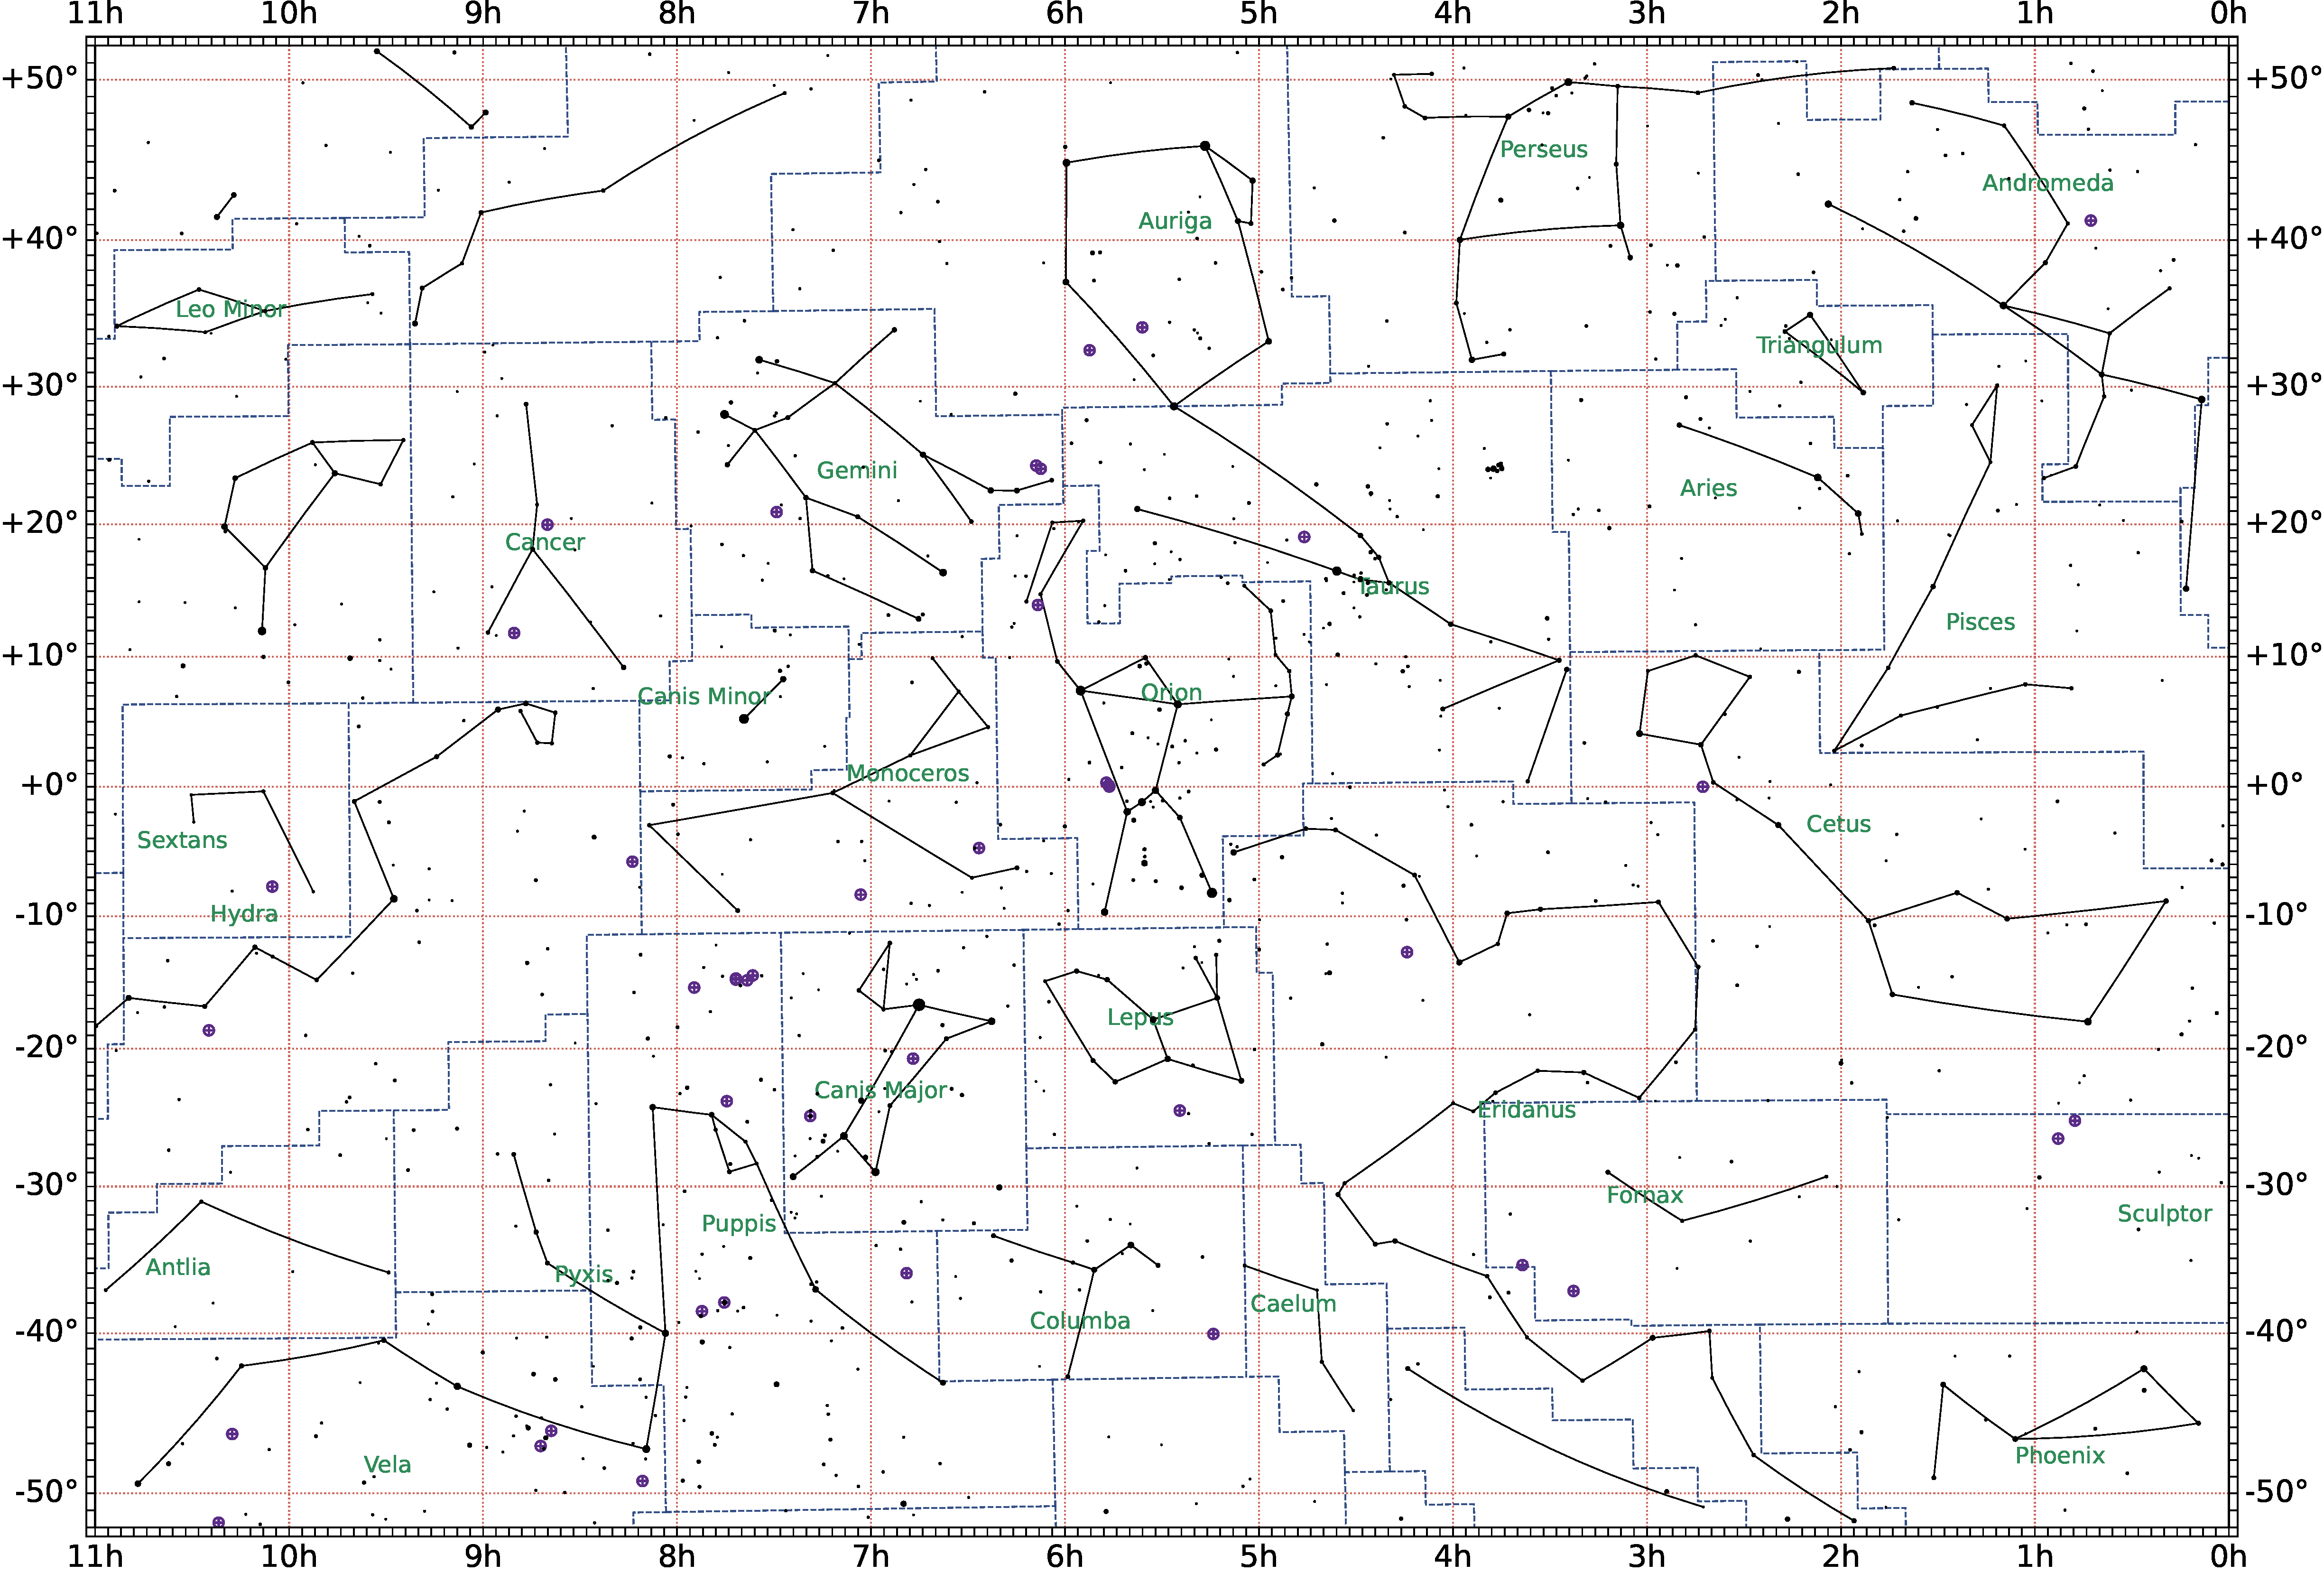
\includegraphics[width=264.0mm]{maps/map1.pdf}}
\end{center}
\clearpage
\begin{center}
\rotatebox{-90}{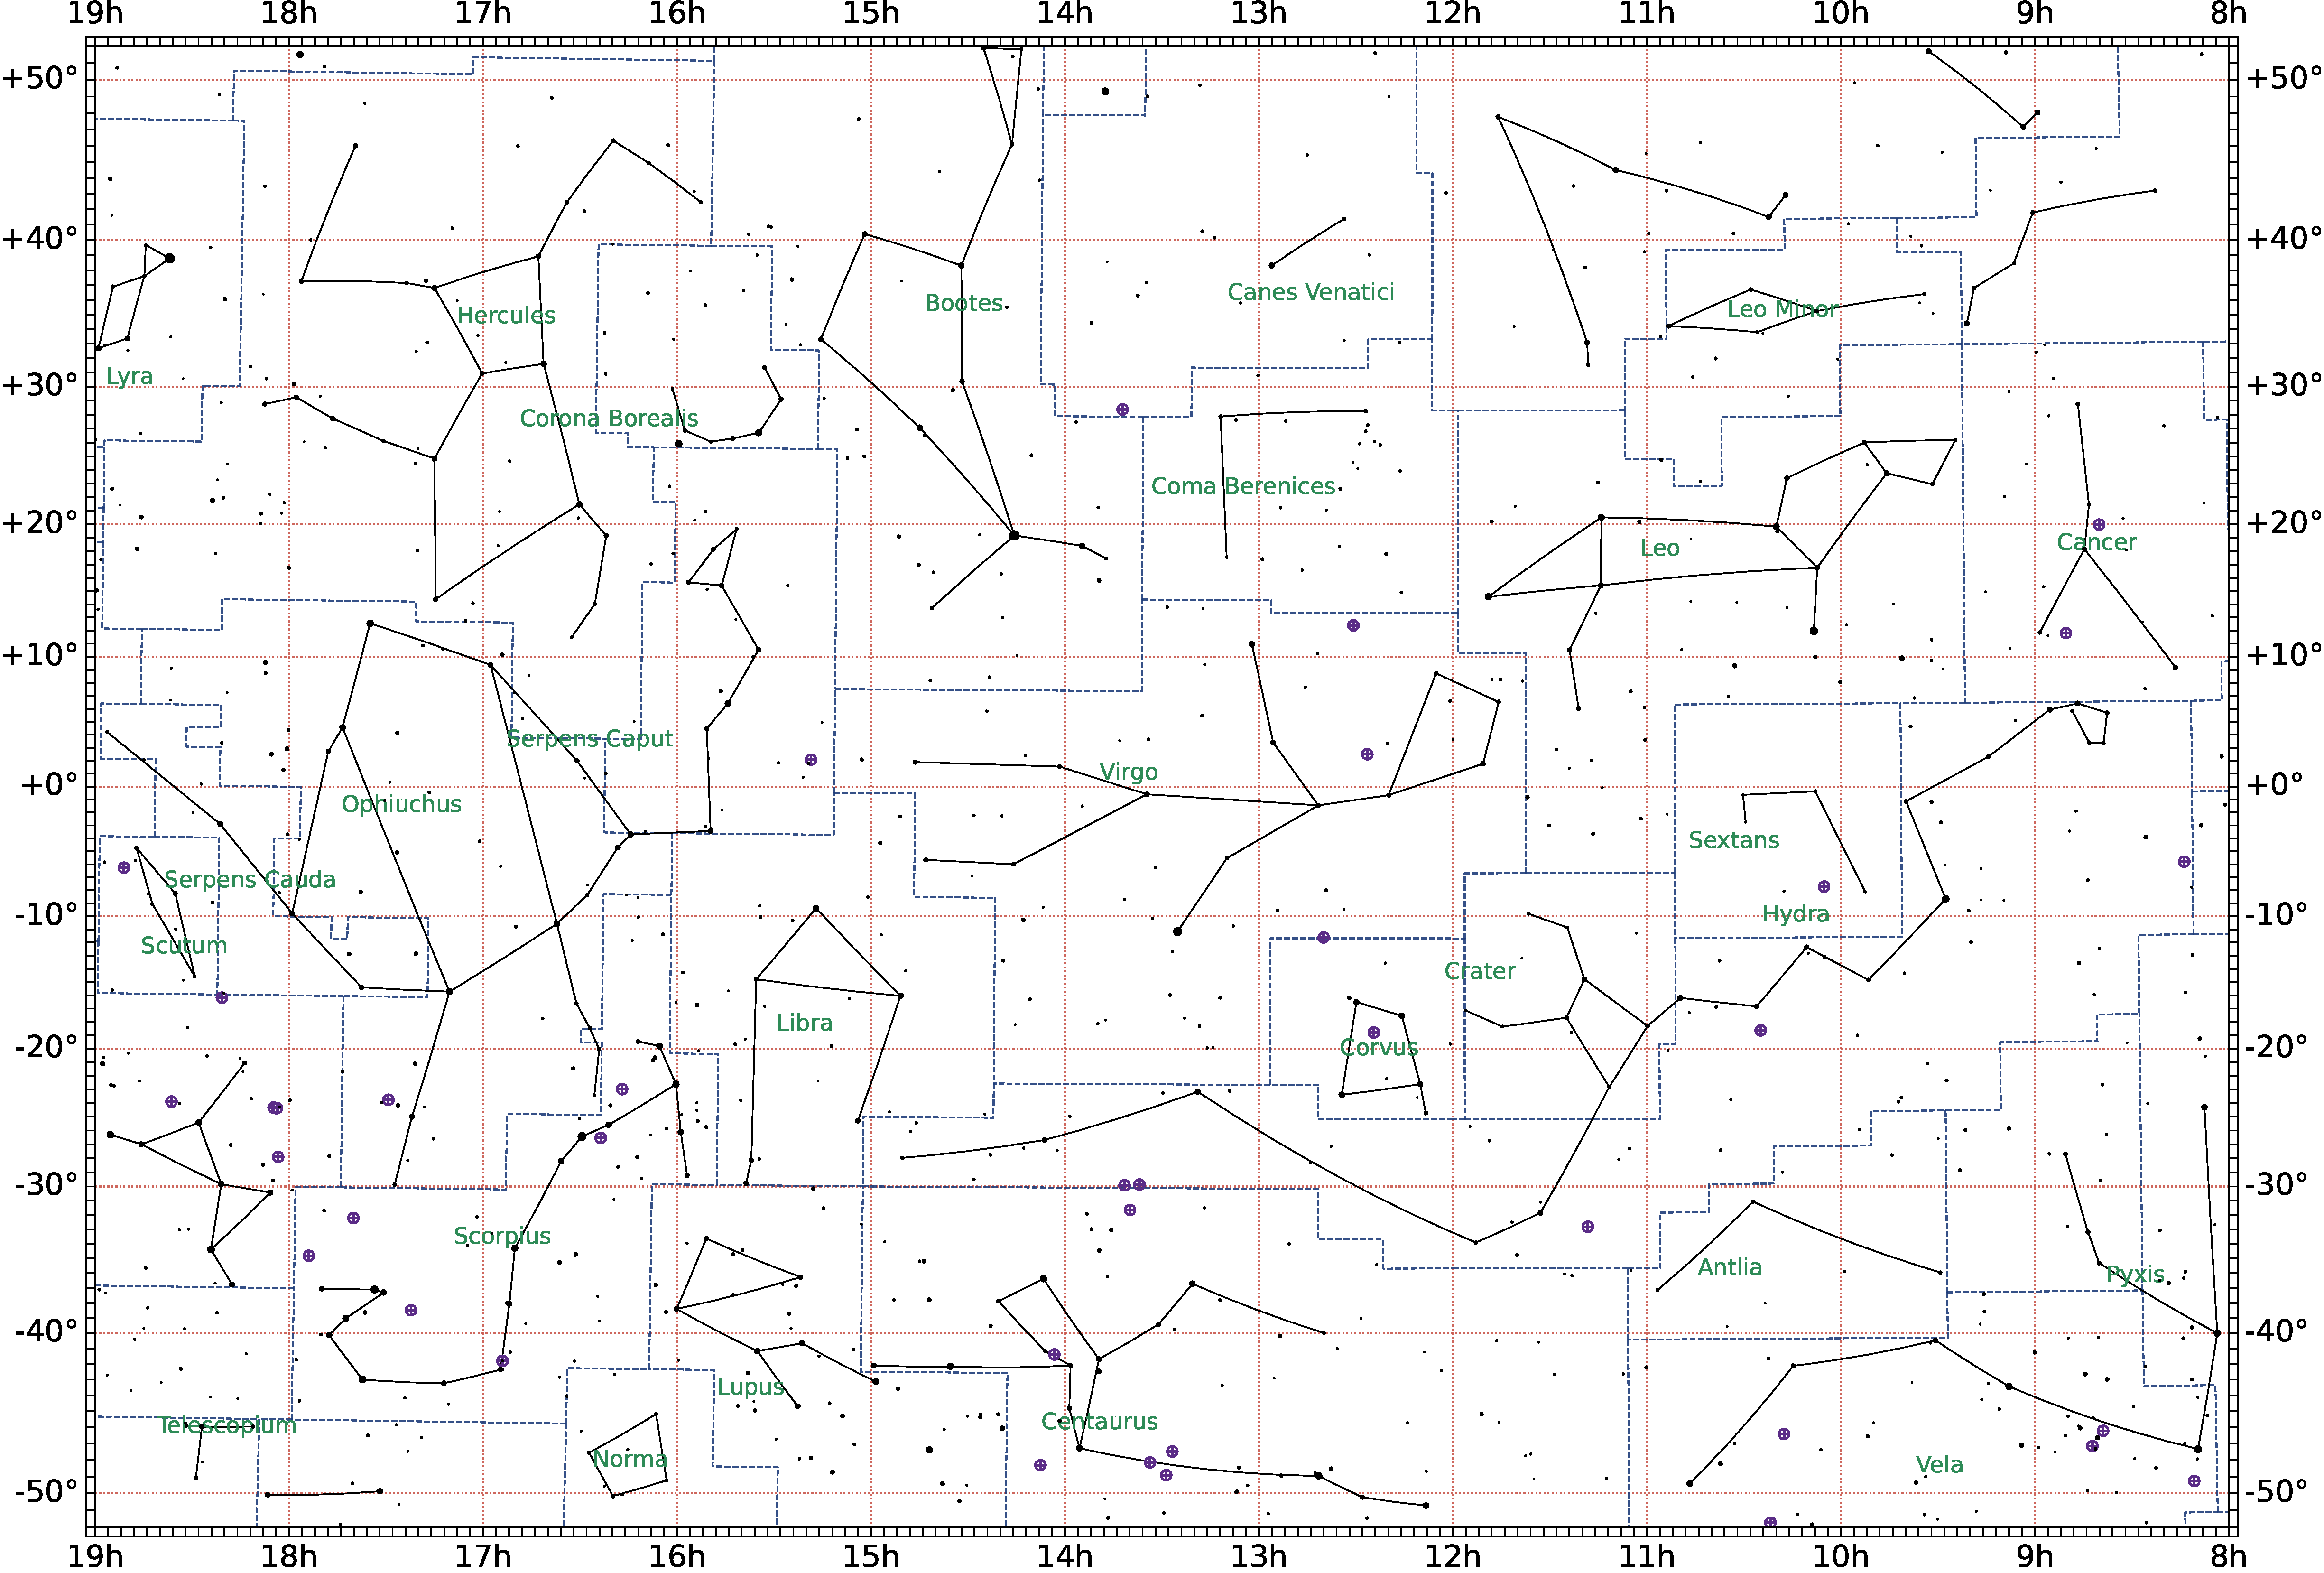
\includegraphics[width=264.0mm]{maps/map2.pdf}}
\end{center}
\clearpage
\begin{center}
\rotatebox{-90}{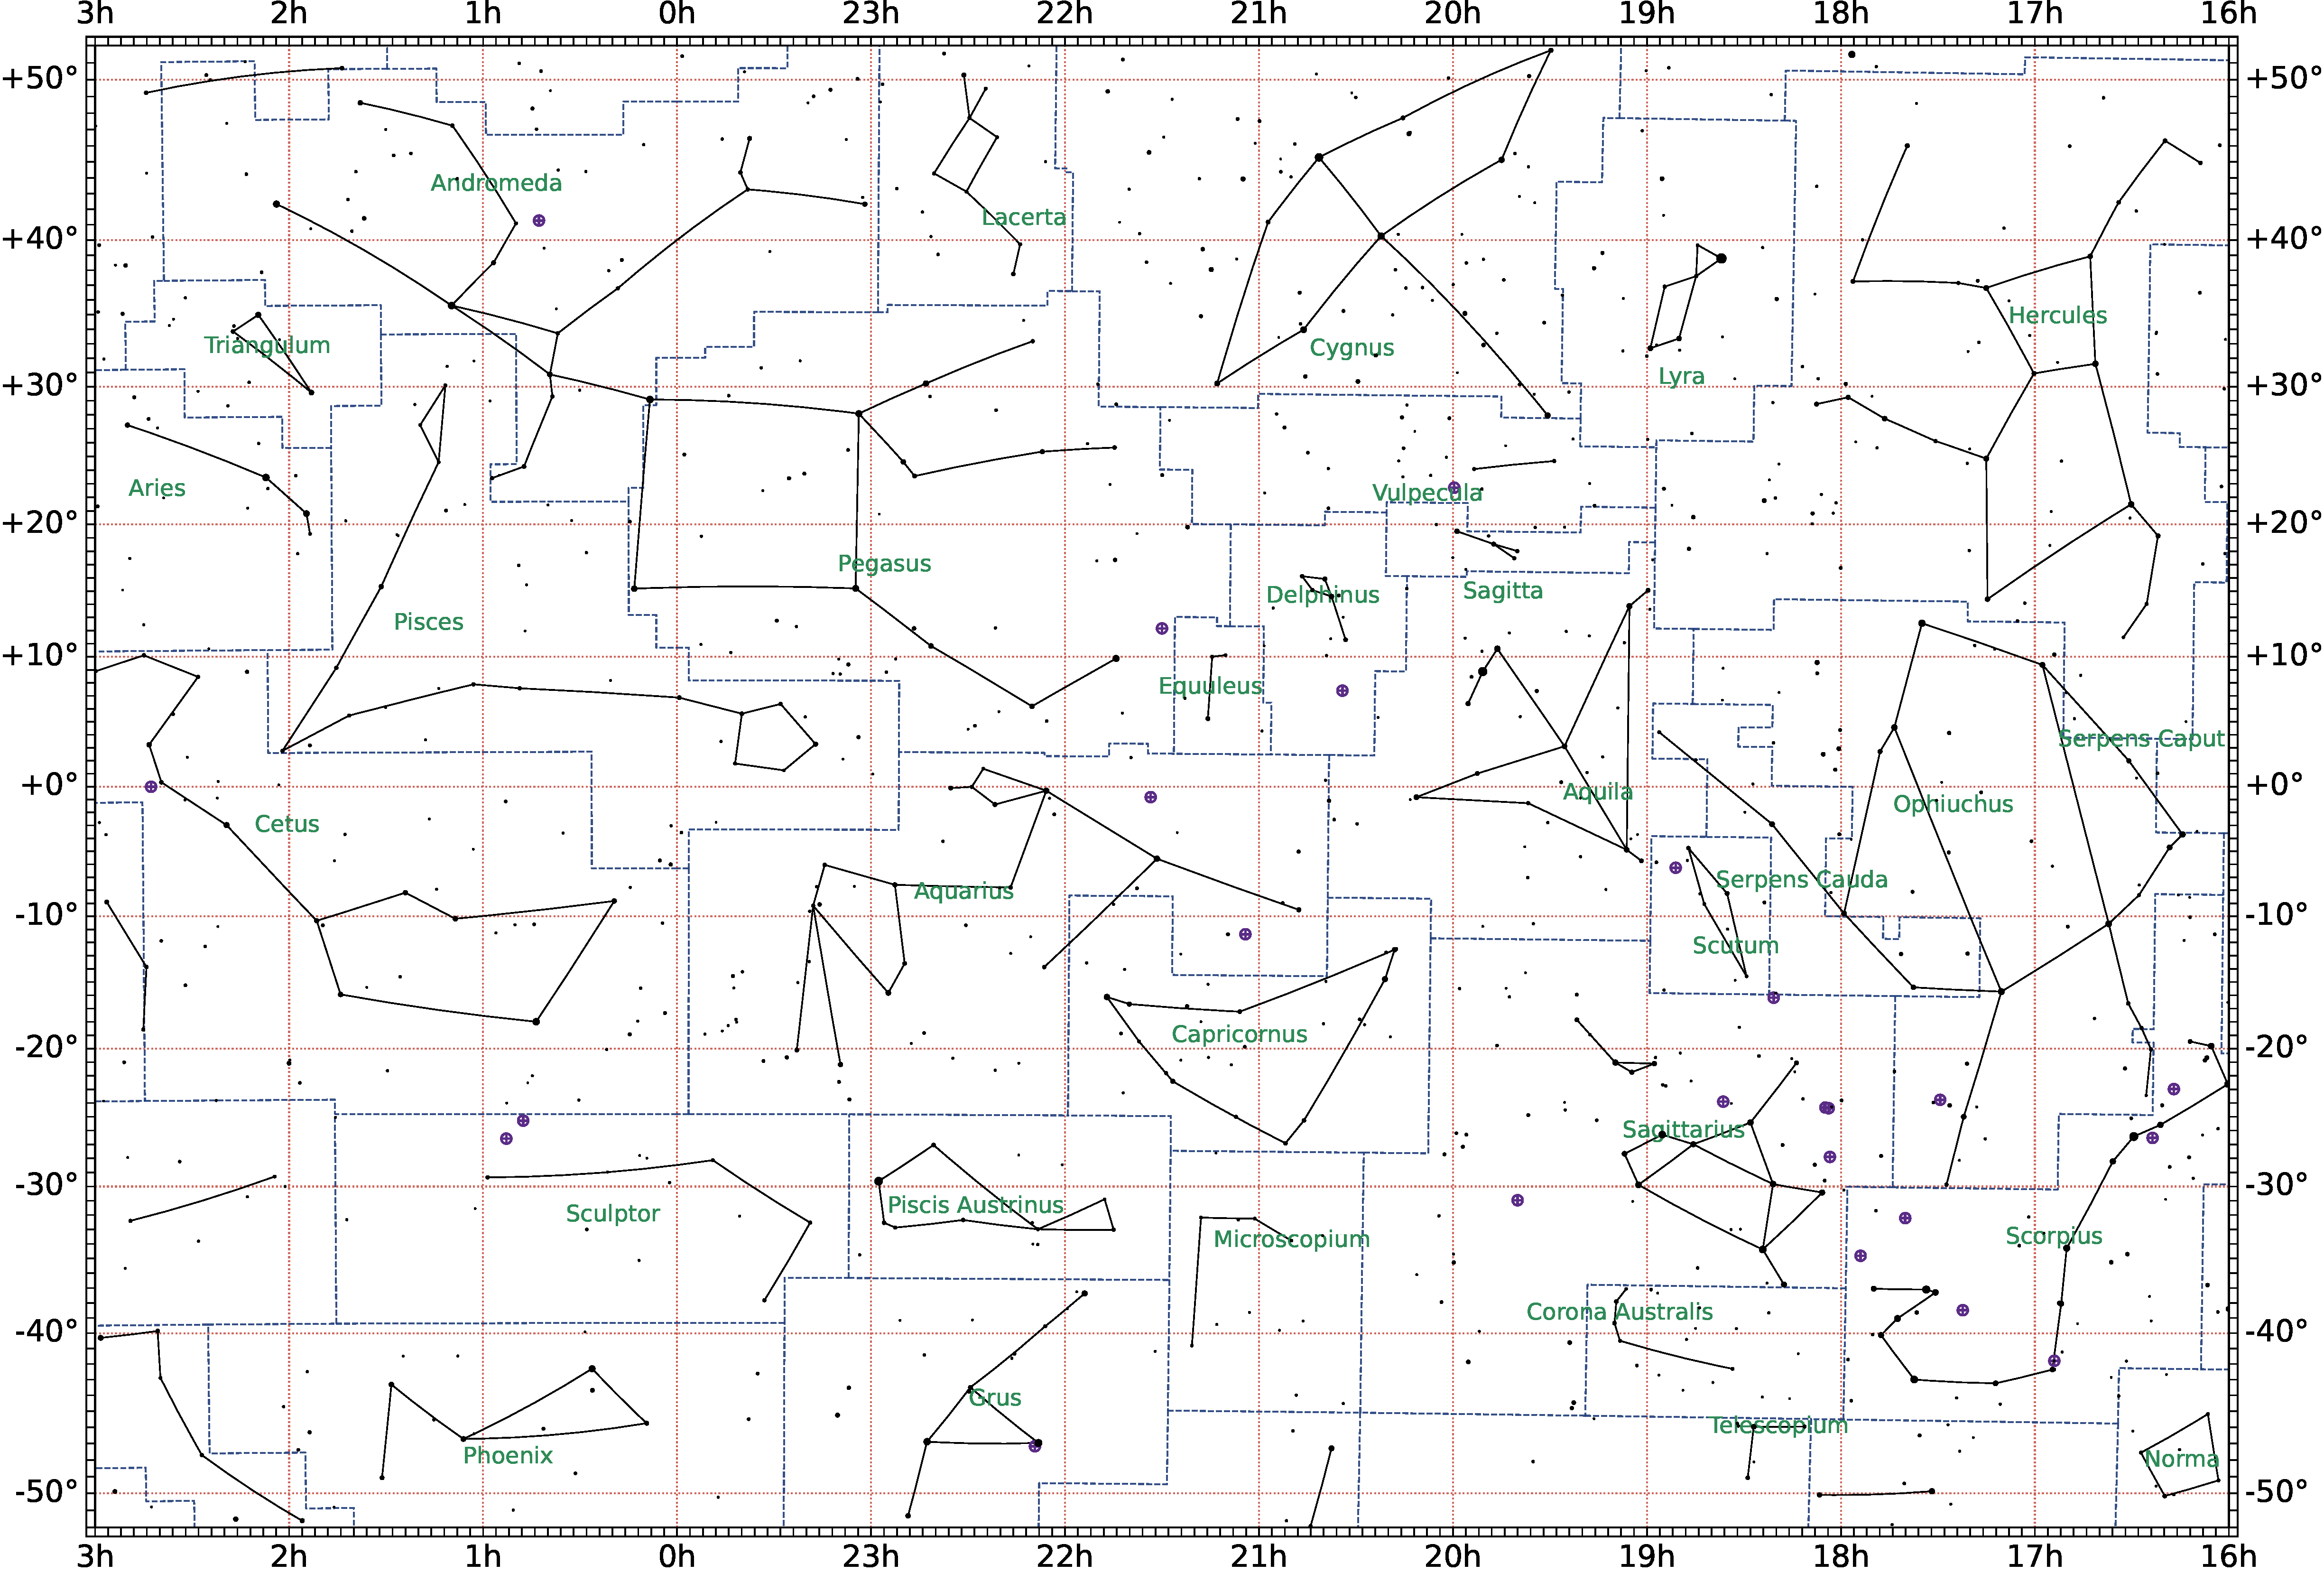
\includegraphics[width=264.0mm]{maps/map3.pdf}}
\end{center}
\clearpage
\ifodd\value{page}\null\clearpage\fi
\noindent\hfill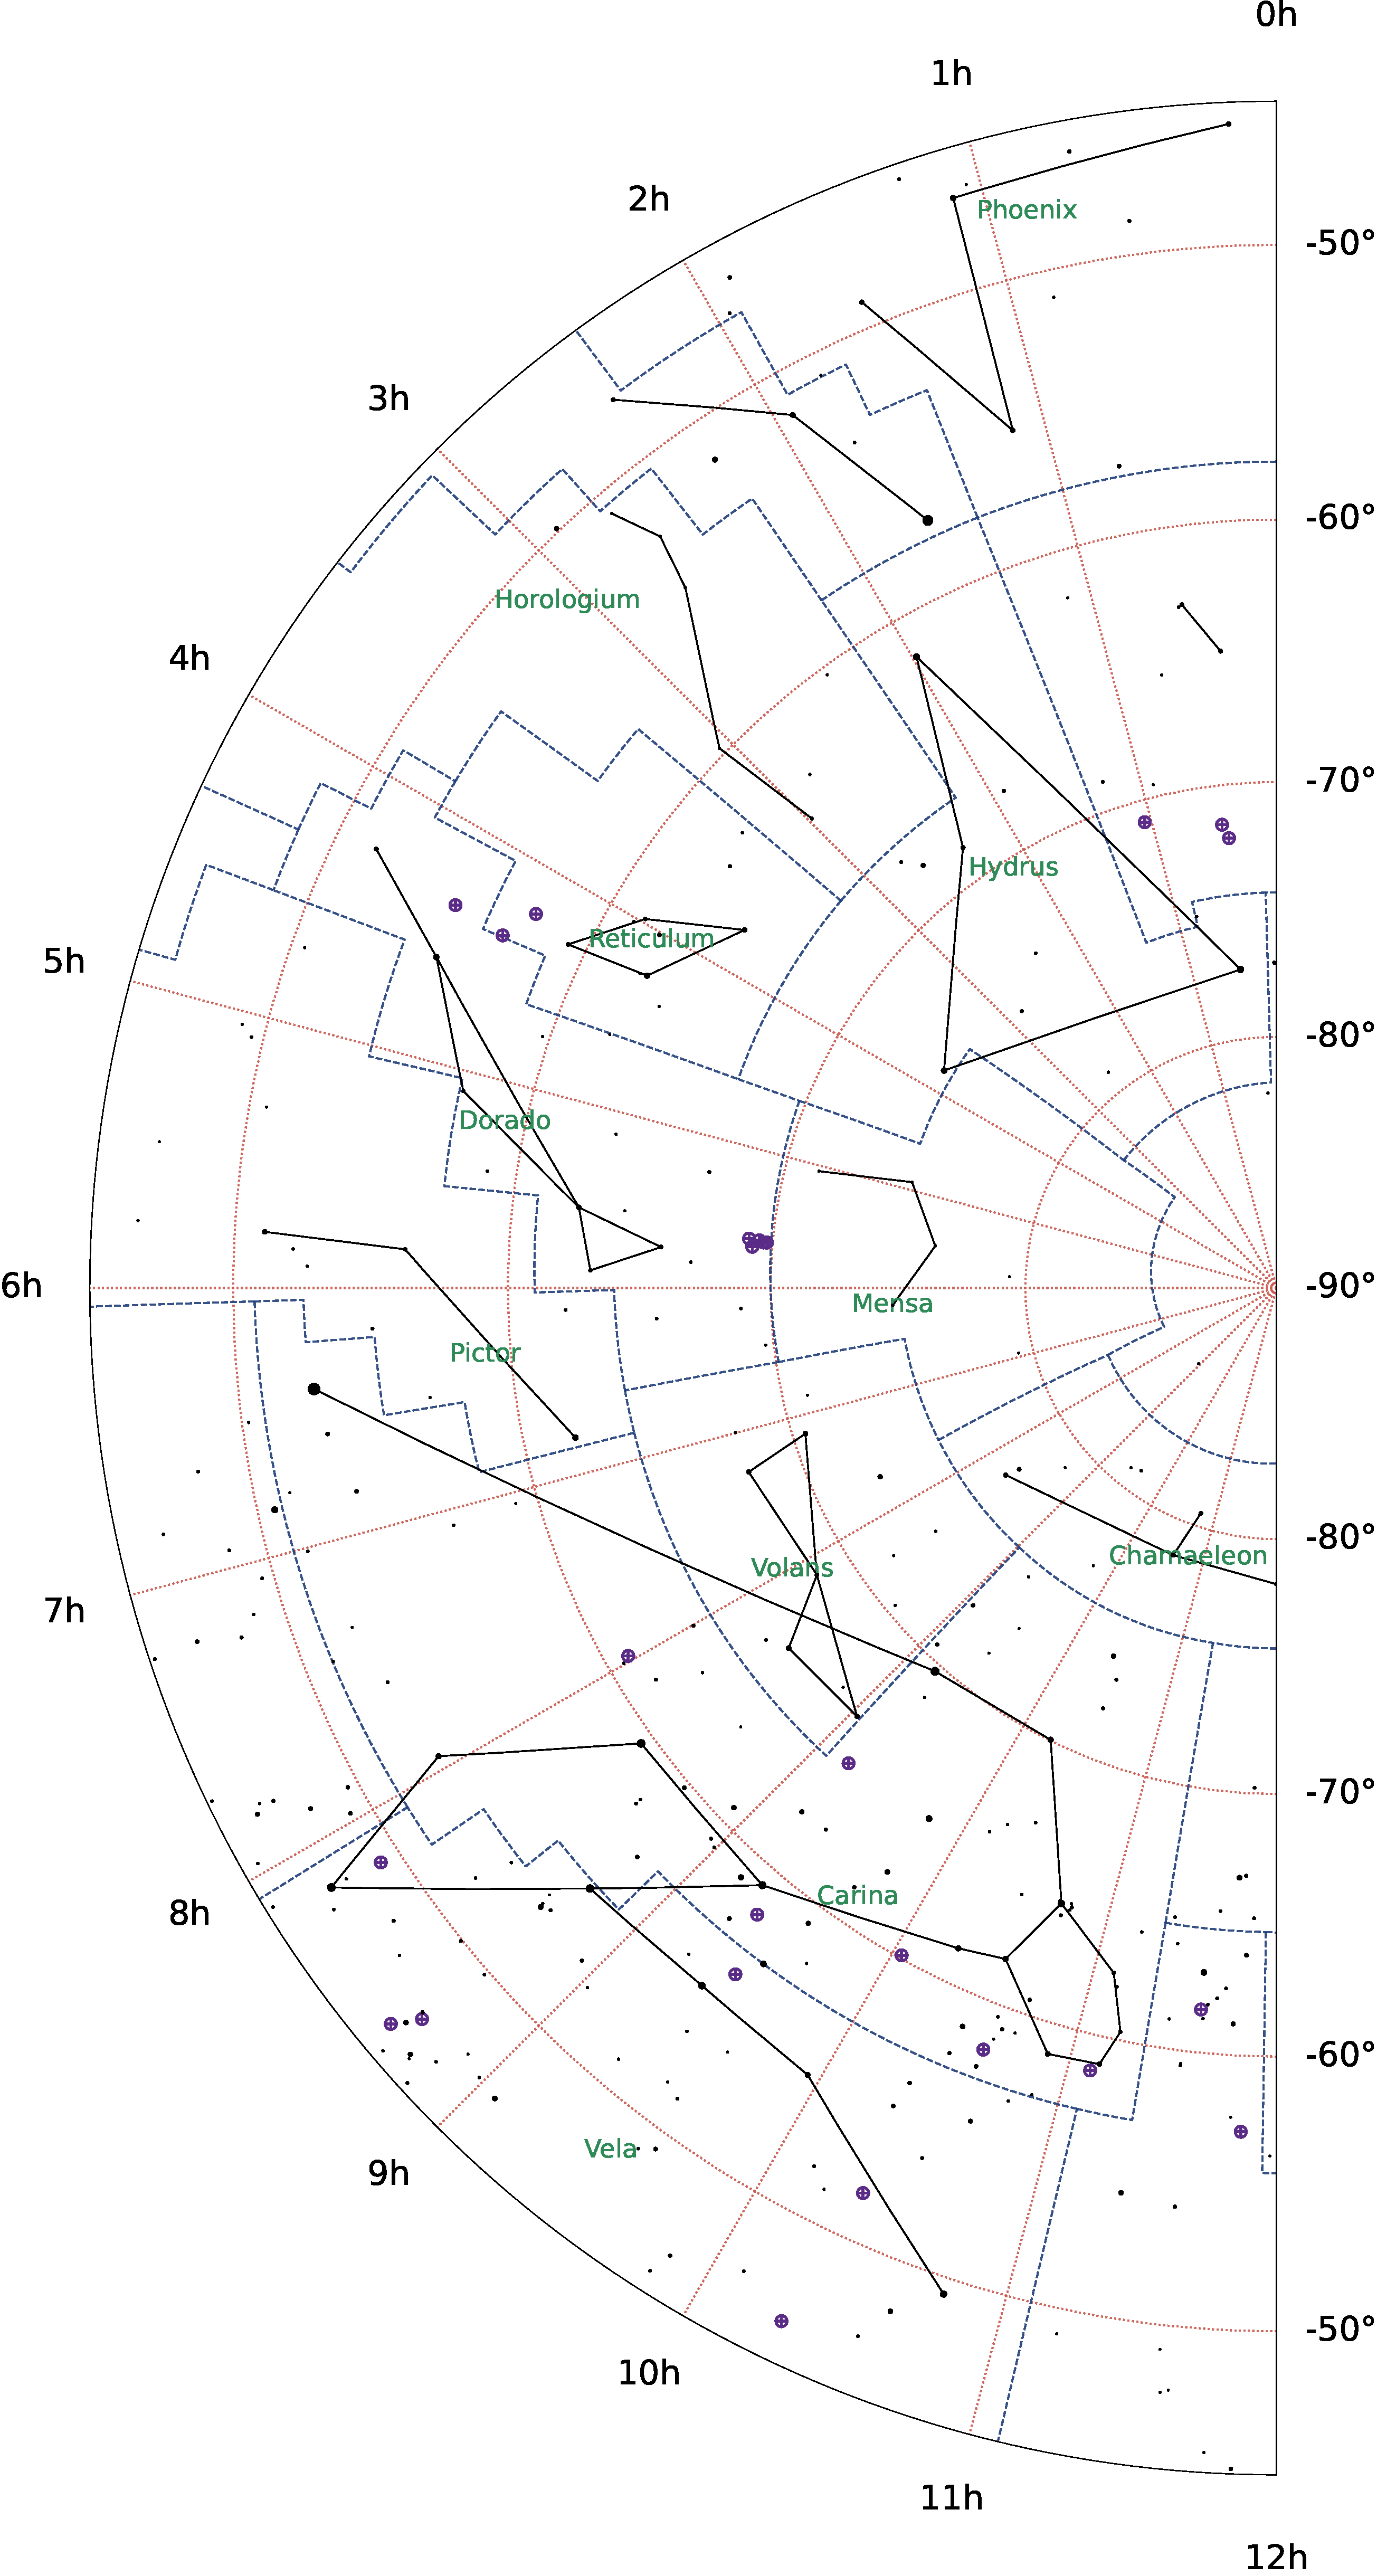
\includegraphics[height=264.0mm]{maps/polar_b.pdf}
\clearpage
\noindent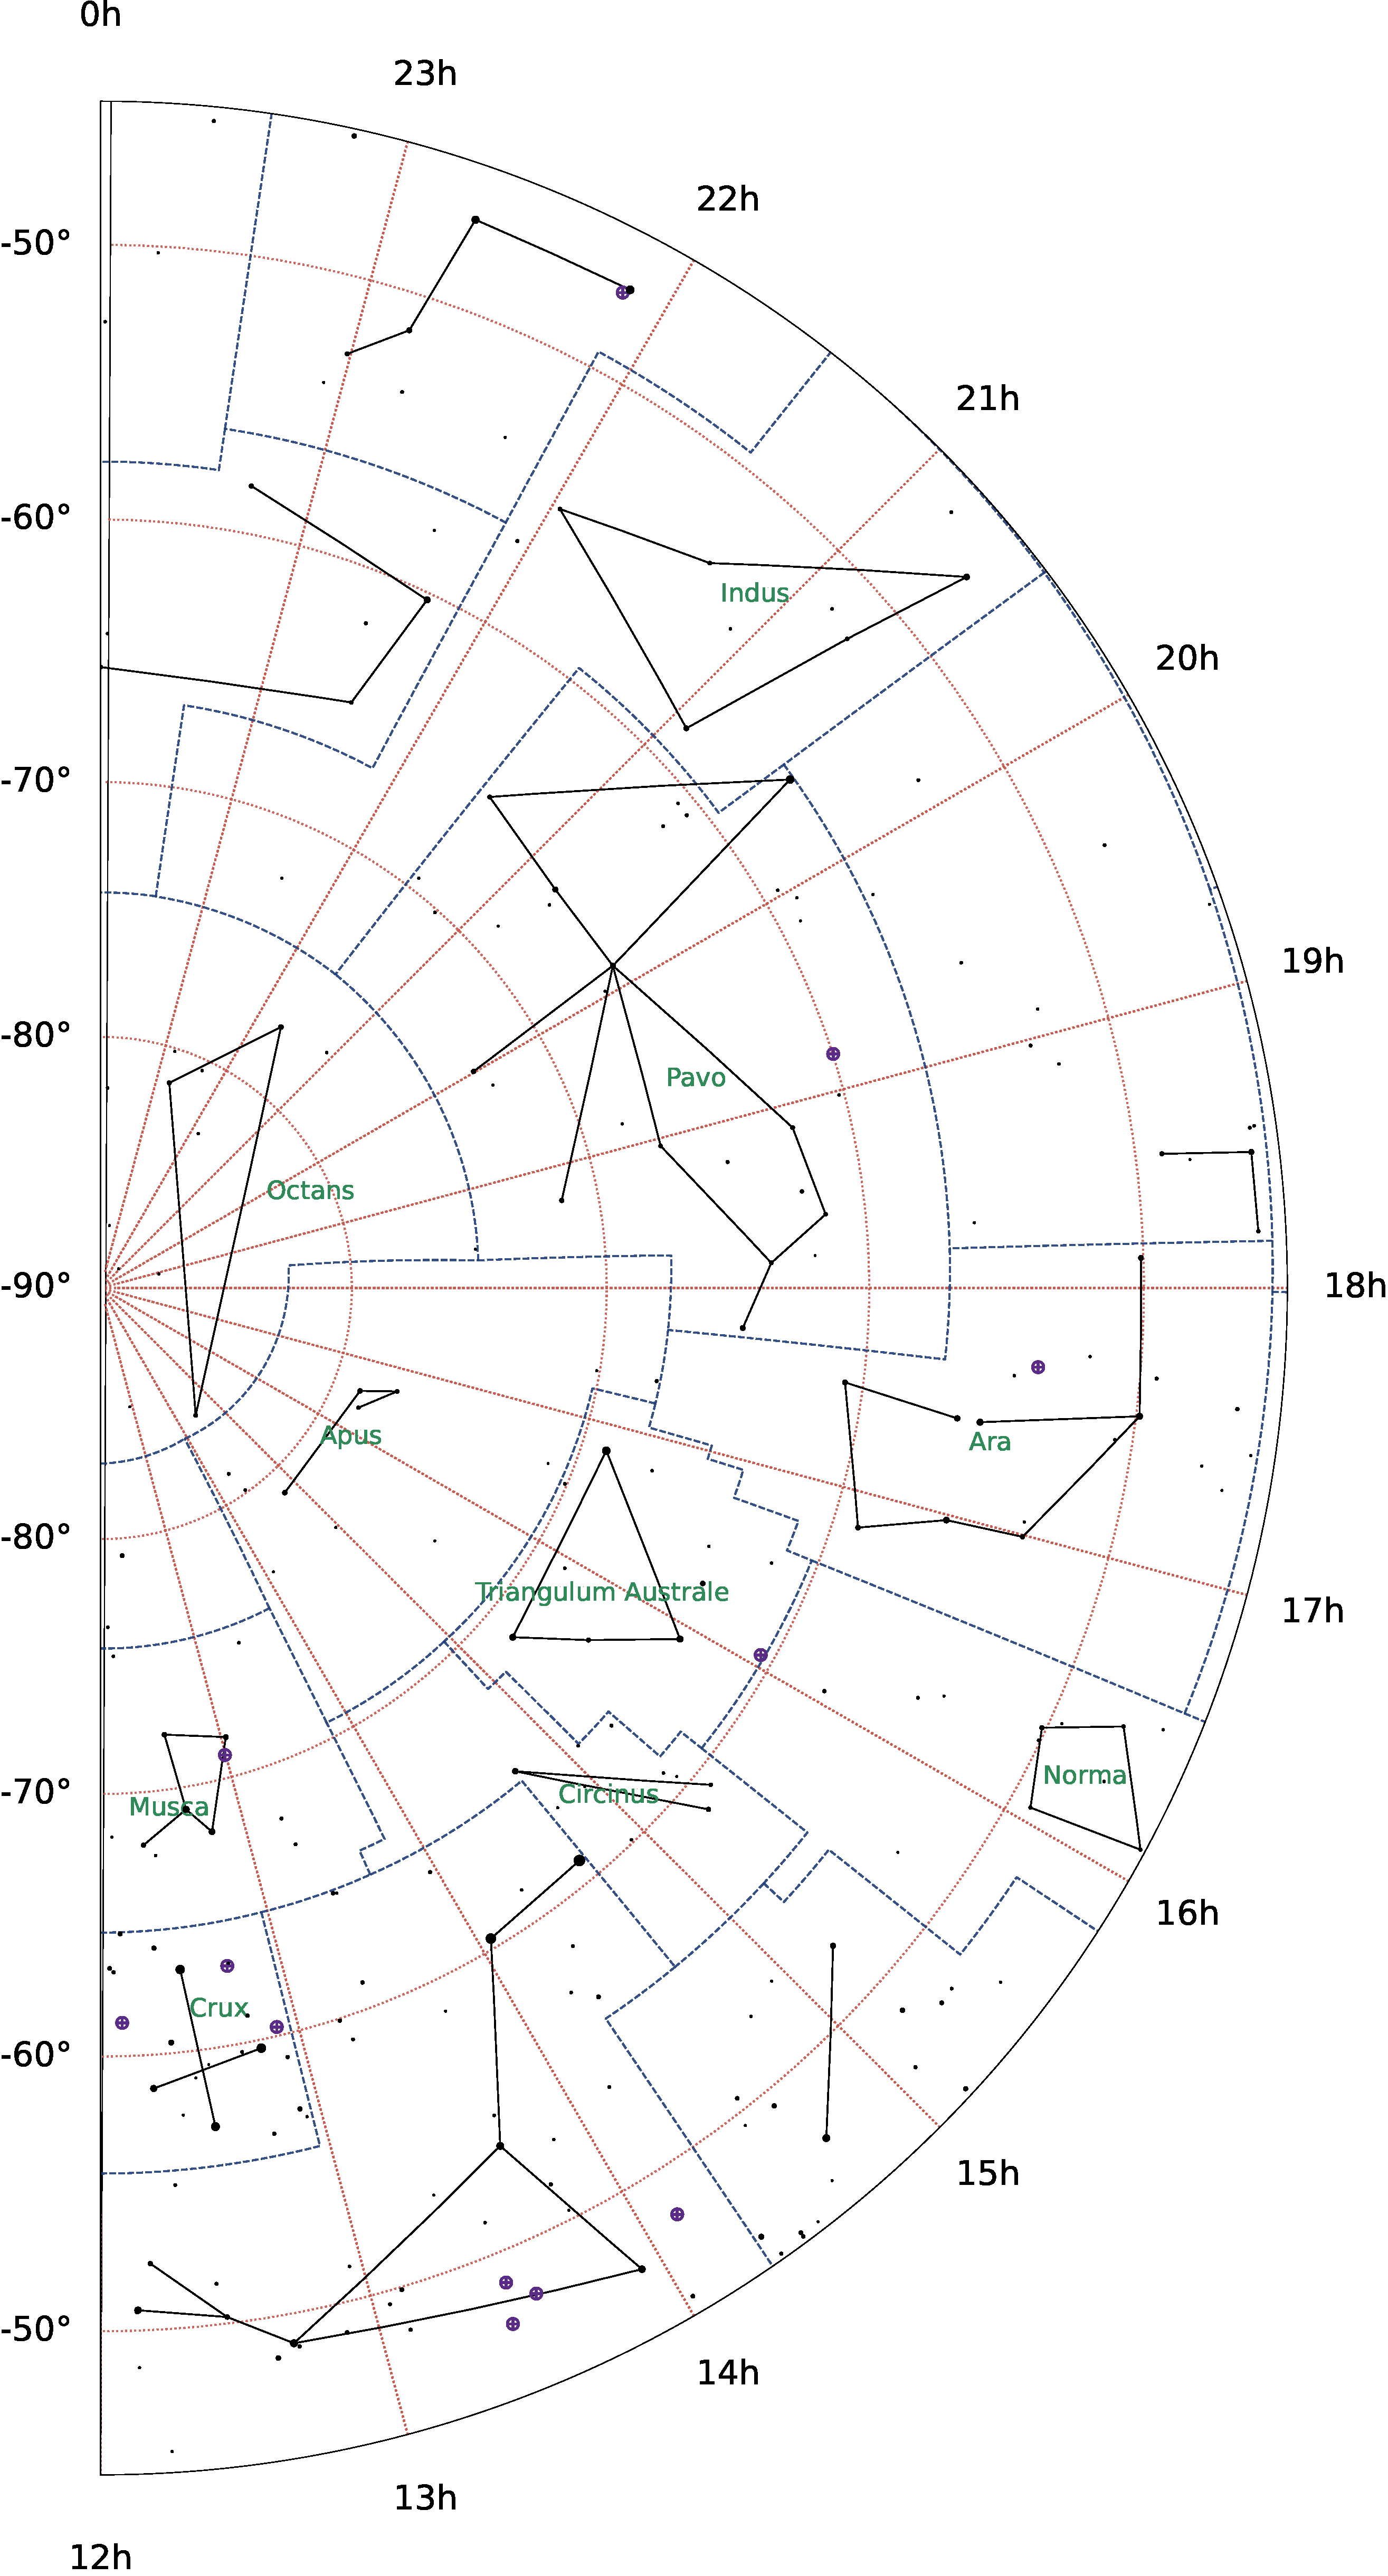
\includegraphics[height=264.0mm]{maps/polar_a.pdf}\hfill\mbox{}
\clearpage
\end{document}
